\documentclass[12pt,a3paper]{article}
\usepackage{pgfplots}
%% ── Packages ──────────────────────────────────────────────────────────
\usepackage{amsmath,amssymb}
\usepackage{amsmath}
\usepackage{geometry}
\usepackage{enumitem}
\usepackage{titlesec}
\usepackage[hidelinks,colorlinks=true,linkcolor=blue!70!black]{hyperref}
\usepackage{xcolor}
\usepackage{fancyhdr}
\usepackage{tcolorbox}
\usepackage{multicol}
\usepackage{needspace}
\usepackage[strings]{underscore}
\usepackage{array,booktabs}
\usepackage[american]{circuitikz}
\usepackage{tikz}
\usepackage{multirow}
\usepackage[table]{xcolor}
\usepackage{tabularx}
\usepackage{caption}
\usepackage{enumitem}

\usetikzlibrary{decorations.pathreplacing}

\usetikzlibrary{shapes.geometric}
\usetikzlibrary{circuits.logic.US, positioning, calc, arrows.meta, decorations.pathreplacing}
\tikzset{every picture/.append style={thick}}
\usetikzlibrary{circuits.logic.US, positioning, calc}
\usetikzlibrary{calc, positioning, backgrounds, fit}
\usetikzlibrary{positioning, arrows.meta, calc, shadows}


\newcounter{myboxcount}

\BeforeBeginEnvironment{tcolorbox}{%
  \stepcounter{myboxcount}% বক্স কাউন্টার ১ বাড়াবে
  \setcounter{equation}{0}% ইকুয়েশন নম্বর ০ করবে (অর্থাৎ ১ থেকে শুরু হবে)
  
  \renewcommand{\theHequation}{\themyboxcount.\arabic{equation}}%
}

% enhanced এবং breakable অপশন সচল করার জন্য লাইব্রেরি
\tcbuselibrary{skins, breakable}


\usetikzlibrary{matrix}
\usetikzlibrary{arrows.meta}
\tcbuselibrary{listings}
\usetikzlibrary{shapes.multipart, positioning, calc, arrows.meta}
\usetikzlibrary{decorations.pathreplacing}
\tcbuselibrary{skins,breakable}
\geometry{margin=2.5cm,headheight=20pt,top=3cm,bottom=3cm}
\tcbset{ansbox/.style={enlarge left by=-\leftmargin, width=\linewidth+\leftmargin}}
\usetikzlibrary{circuits.logic.US}


%% ── Colors ────────────────────────────────────────────────────────────
\definecolor{pblue}{RGB}{13,71,161}
\definecolor{dgray}{RGB}{66,66,66}
\definecolor{cA}{RGB}{0,77,64}
\definecolor{cB}{RGB}{1,87,155}
\definecolor{cC}{RGB}{27,94,32}
\definecolor{cD}{RGB}{106,27,154}
\definecolor{cE}{RGB}{230,81,0}
\definecolor{cF}{RGB}{0,96,100}
\definecolor{cH}{RGB}{0,77,64}
\definecolor{cG}{RGB}{136,14,79}
\definecolor{cI}{RGB}{62,39,35}

%% ── Section headings ──────────────────────────────────────────────────
\titleformat{\section}{\large\bfseries\color{pblue}}{}{0em}{}[\titlerule]
\titleformat{\subsection}{\normalsize\bfseries}{}{0em}{}

%% ── Header / Footer ───────────────────────────────────────────────────
\pagestyle{fancy}\fancyhf{}
\renewcommand{\headrulewidth}{0.5pt}
\fancyhead[L]{\small\textcolor{pblue}{\textbf{BUET $|$ Electronic Circuits Question Bank}}}
\fancyhead[R]{\small\textcolor{dgray}{\textit{\nouppercase{\leftmark}}}}
\fancyfoot[C]{\small\thepage}

%% ── Utility macros ────────────────────────────────────────────────────
\newcommand{\yr}[1]{\hfill\textcolor{gray}{\small\textbf{[#1]}}}
\newcommand{\mk}[1]{\textcolor{orange!70!black}{\small\textbf{(#1 marks)}}}
\newcommand{\variant}[1]{\par\vspace{1pt}\textcolor{blue!50!black}%
  {\footnotesize\textit{$\hookrightarrow$ Similar: #1}}}
\newcommand{\diagram}{\par\vspace{4pt}\textcolor{gray!55}{\small\textit{[Diagram to be added manually]}}}

%% ── Subtopic heading macro ────────────────────────────────────────────
\newcommand{\subtopic}[2]{%
  \vspace{10pt}
  \noindent\begin{tcolorbox}[colback=#1!8,colframe=#1,boxrule=0.6pt,arc=4pt,
    left=6pt,right=6pt,top=4pt,bottom=4pt]
    \small\bfseries\textcolor{#1}{#2}
  \end{tcolorbox}
  \vspace{2pt}
}

\ctikzset{tripoles/mos style/arrows}

%% ── Section divider page ──────────────────────────────────────────────
\newcommand{\secdivider}[3]{%
  \newpage\thispagestyle{empty}%
  \vspace*{\fill}%
  \begin{tcolorbox}[enhanced,colback=#3!6,colframe=#3,boxrule=1.5pt,arc=8pt,
    left=20pt,right=20pt,top=22pt,bottom=22pt,
    shadow={3pt}{-3pt}{0pt}{black!15}]
    \centering
    {\large\textcolor{gray}{\textbf{BUET $\cdot$ EEE 263 $\cdot$ Electronic Circuits}}}\\[8pt]
    {\fontsize{26}{32}\selectfont\bfseries\textcolor{#3}{Electronic Circuits}}\\[6pt]
    {\fontsize{15}{19}\selectfont\textcolor{dgray}{#1}}\\[12pt]
    \textcolor{#3!60}{\rule{0.5\textwidth}{0.5pt}}\\[6pt]
    {\small\textcolor{gray}{#2}}
  \end{tcolorbox}%
  \vspace*{\fill}\newpage%
}

%% ── List styles ───────────────────────────────────────────────────────
\setlist[enumerate,1]{label=\textbf{Q\arabic*.},leftmargin=*,itemsep=14pt,parsep=2pt}
\setlist[enumerate,2]{label=(\alph*),leftmargin=2em,itemsep=3pt}
\setlist[enumerate,3]{label=(\roman*),leftmargin=2.5em,itemsep=2pt}




\begin{document}

%% ══════════════════════════════════════════════════════════════════════
%%  COVER PAGE
%% ══════════════════════════════════════════════════════════════════════
\thispagestyle{empty}
\begin{tcolorbox}[enhanced,colback=cA!5,colframe=cA,boxrule=1.5pt,arc=6pt,
  top=28pt,bottom=28pt,left=22pt,right=22pt,
  shadow={4pt}{-4pt}{0pt}{black!20}]
  \centering
  
  % --- BUET Logo Added Here ---
  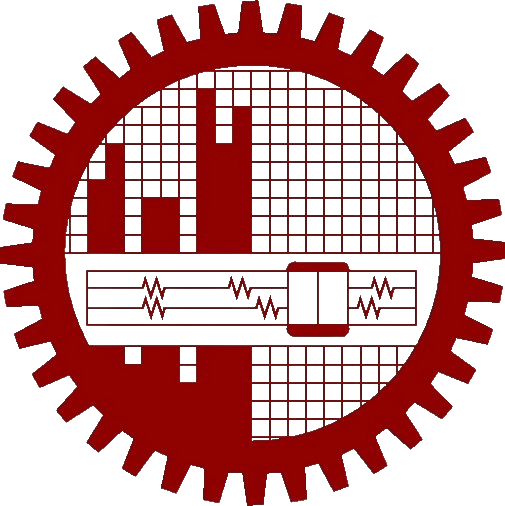
\includegraphics[height=2.5cm]{images/buet_logo.png}\\[8pt]
  % ----------------------------
  
  {\Large\bfseries\textcolor{cA}{Bangladesh University of Engineering and Technology}}\\[4pt]
  {\normalsize\textcolor{dgray}{Department of Computer Science \& Engineering}}\\[18pt]
  \textcolor{cA}{\rule{\textwidth}{1pt}}\\[14pt]
  
  {\fontsize{22}{28}\selectfont\bfseries\textcolor{cA}{Electronic Circuits Question Bank\\With Answers}}\\[8pt]
  {\fontsize{14}{18}\selectfont\textcolor{dgray}{EEE 263 $\cdot$ Electronic Circuits}}\\[4pt]
  \textcolor{cA}{\rule{\textwidth}{0.5pt}}\\[14pt]
  
  {\small\textcolor{dgray}{Year Coverage:\;2011-12 to 2024--25\\Topics:\;Diode Characteristics, Wave Shaping \& Clipping/Clamping,\\
  BJT \& MOSFET Amplifiers, Op-Amps (Filters, Schmitt Trigger, Analog Computing), Oscillators \& Timers (555) \& more}}\\[16pt]
  

    {\small\bfseries\textcolor{dgray}{Authors \& Contributors}}\\[6pt]
    \begin{tabular}{rl}
        \textcolor{dgray}{\textbf{Md Ratul Hasan}} \textcolor{dgray}{\small(2405009)} & --- Question Curation \& Organisation\\
      & --- \LaTeX\ Typesetting\\[3pt]
            \textbf{NotebookLM} & --- Research \& Extraction\\[3pt]
      \textbf{Claude AI} & --- \LaTeX\ Typesetting\\[3pt]
      \textbf{Gemini} & --- Answer \& Diagram Generation\\[3pt]
       \end{tabular}
 
\end{tcolorbox}
\newpage

%% ══════════════════════════════════════════════════════════════════════
%%  TABLE OF CONTENTS
%% ══════════════════════════════════════════════════════════════════════
\thispagestyle{fancy}\markboth{Table of Contents}{}
\begin{center}
  {\LARGE\bfseries\textcolor{pblue}{Table of Contents}}\\[6pt]
  \textcolor{pblue}{\rule{0.6\textwidth}{0.8pt}}
\end{center}
\vspace{6pt}

%% Part I
\begin{tcolorbox}[breakable,colback=cA!5,colframe=cA,boxrule=1pt,arc=5pt,
  left=8pt,right=8pt,top=8pt,bottom=8pt,before skip=4pt]
  {\large\bfseries\textcolor{cA}{Part I --- Diode}}\\[5pt]
  \textcolor{cA!40}{\rule{\textwidth}{0.4pt}}\\[3pt]
  \small\begin{itemize}[leftmargin=1.2em,itemsep=1pt,label={\textcolor{cA}{$\triangleright$}}]
    \item \hyperref[sec:S1]{\textbf{S1.} Diode Characteristics}
      \begin{itemize}[leftmargin=1.5em,itemsep=0pt,label={\textcolor{cA}{$\cdot$}}]
        \item \hyperref[sub:s1-dc]{Diode Circuit Analysis}
        \item \hyperref[sub:s1-models]{Diode Models (Ideal, CVD, Piecewise Linear)}
        \item \hyperref[sub:s1-ssm]{Small Signal Model}
        \item \hyperref[sub:s1-peak]{Peak Rectifier}
        \item \hyperref[sub:s1-iv]{I-V Characteristics \& Waveform Analysis}
        \item \hyperref[sub:s1-thermal]{Diode Thermal Characteristics}
        \item \hyperref[sub:s1-rectifier]{Bridge Rectifier}
        \item \hyperref[sub:s1-zener]{Zener Diode Regulator}
        \item \hyperref[sub:s1-battery]{Battery Charger Circuit}
        \item \hyperref[sub:s1-spd]{Special Purpose Diodes/Thyristors}
        \item \hyperref[sub:s1-Miscellaneous]{Miscellaneous}
      \end{itemize}

      \item \hyperref[sec:S2]{\textbf{S2.} Clipping, Clamping Circuits}
      \begin{itemize}[leftmargin=1.5em,itemsep=0pt,label={\textcolor{cB}{$\cdot$}}]
        \item \hyperref[sub:s2-clipping]{Clipping Circuits --- Waveform \& Transfer Characteristics}
        \item \hyperref[sub:s2-clamping]{Clamping Circuits}
        
      \end{itemize}


  \end{itemize}
\end{tcolorbox}

\vspace{6pt}



%% Part II
\begin{tcolorbox}[breakable,colback=cC!5,colframe=cC,boxrule=1pt,arc=5pt,
  left=8pt,right=8pt,top=8pt,bottom=8pt,before skip=4pt]
  {\large\bfseries\textcolor{cC}{Part II --- Bipolar Junction Transistors (BJTs)}}\\[5pt]
  \textcolor{cC!40}{\rule{\textwidth}{0.4pt}}\\[3pt]
  \small\begin{itemize}[leftmargin=1.2em,itemsep=1pt,label={\textcolor{cC}{$\triangleright$}}]

    \item \hyperref[sec:S3]{\textbf{S3.} BJT Characteristics}
      \begin{itemize}[leftmargin=1.5em,itemsep=0pt,label={\textcolor{cA}{$\cdot$}}]
        \item \hyperref[sub:s3-energy]{Energy Band Profile}
        \item \hyperref[sub:s3-structure]{Device Structure and Operating Principle}
        \item \hyperref[sub:s3-early]{Early Effect}
        \item \hyperref[sub:s3-dc]{DC Analysis}
        \item \hyperref[sub:s3-saturation]{BJT Saturation Parameters}
        \item \hyperref[sub:s3-multibjtdc]{Multi-BJT Circuit Analysis}
        \item \hyperref[sub:s3-vtc]{Voltage Transfer Characteristics}
        \item \hyperref[sub:s3-opmode]{Operating Mode Design}
        \item \hyperref[sub:s3-biasing]{Biasing and Stability}
        \item \hyperref[sub:s3-design]{BJT Circuit Design}
        \item \hyperref[sub:s3-linear]{Linear Amplifier Constraints}
        
        \item \hyperref[sub:s3-switching]{Switching Circuits --- Logic Gates using BJTs}
        \item \hyperref[sub:s3-inverter]{BJT Inverter Analysis}
      \end{itemize}
    \item \hyperref[sec:S4]{\textbf{S4.} BJT Amplifiers}
      \begin{itemize}[leftmargin=1.5em,itemsep=0pt,label={\textcolor{cC}{$\cdot$}}]
        \item \hyperref[sub:s4-ce]{Common Emitter / Trans-conductance Amplifier}
        \item \hyperref[sub:s4-cb]{Common Base Amplifier}
        \item \hyperref[sub:s4-bootstrap]{Bootstrapped Follower}
        \item \hyperref[sub:s4-cc]{Common Collector (Emitter Follower)}
        \item \hyperref[sub:s4-biasimpedance]{Biasing and Input Impedance}
        \item \hyperref[sub:s4-io]{BJT Input-Output Characteristics}
      \end{itemize}

  \end{itemize}
\end{tcolorbox}

\vspace{6pt}


%% Part III
\begin{tcolorbox}[breakable,colback=cB!5,colframe=cB,boxrule=1pt,arc=5pt,
  left=8pt,right=8pt,top=8pt,bottom=8pt,before skip=4pt]
  {\large\bfseries\textcolor{cB}{Part III --- MOS Field-Effect Transistors
(MOSFETs)}}\\[5pt]
  \textcolor{cB!40}{\rule{\textwidth}{0.4pt}}\\[3pt]
  \small\begin{itemize}[leftmargin=1.2em,itemsep=1pt,label={\textcolor{cB}{$\triangleright$}}]

        \item \hyperref[sec:S5]{\textbf{S5.} MOSFET Characteristics}
      \begin{itemize}[leftmargin=1.5em,itemsep=0pt,label={\textcolor{cA}{$\cdot$}}]
        \item \hyperref[sub:s5-devchar]{Device Characteristics}
        \item \hyperref[sub:s5-compare]{Comparison with BJT}
        \item \hyperref[sub:s5-threshold]{Threshold Voltage}
        \item \hyperref[sub:s5-dc]{DC Analysis \& Transistor Sizing}
        \item \hyperref[sub:s5-multistage]{Multi-stage MOSFET Circuit Design}
        \item \hyperref[sub:s5-gm]{MOSFET Transconductance}
        \item \hyperref[sub:s5-vtc]{Voltage Transfer Characteristics}
        \item \hyperref[sub:s5-ssa]{MOSFET as Small-Signal Amplifier}
        \item \hyperref[sub:s5-biasing]{Biasing Stability}
        \item \hyperref[sub:s5-cmos]{CMOS Logic Implementation}
        \item \hyperref[sub:s5-sizing]{CMOS Sizing and Delay}
        \item \hyperref[sub:s5-nmos]{NMOS Circuit Design}
        \item \hyperref[sub:s5-cmos]{CMOS Inverter Analysis}
            
      \end{itemize}
    \item \hyperref[sec:S6]{\textbf{S6.} MOSFET Amplifiers}
      \begin{itemize}[leftmargin=1.5em,itemsep=0pt,label={\textcolor{cC}{$\cdot$}}]
        \item \hyperref[sub:s6-cg]{Common Gate Amplifier}
        \item \hyperref[sub:s6-cs]{Common Source Amplifier}
      \end{itemize}
      
      
  \end{itemize}
\end{tcolorbox}

\vspace{6pt}

%% Part IV
\begin{tcolorbox}[breakable,colback=cE!5,colframe=cE,boxrule=1pt,arc=5pt,
  left=8pt,right=8pt,top=8pt,bottom=8pt,before skip=4pt]
  {\large\bfseries\textcolor{cE}{Part IV --- Linear Integrated Circuits (Op-Amps)}}\\[5pt]
  \textcolor{cE!40}{\rule{\textwidth}{0.4pt}}\\[3pt]
  \small\begin{itemize}[leftmargin=1.2em,itemsep=1pt,label={\textcolor{cE}{$\triangleright$}}]
    \item \hyperref[sec:S7]{\textbf{S7.} Operational Amplifiers (Op-Amps)}
      \begin{itemize}[leftmargin=1.5em,itemsep=0pt,label={\textcolor{cE}{$\cdot$}}]
        \item \hyperref[sub:s7-ideal]{Ideal Op-Amp Characteristics}
        \item \hyperref[sub:s7-math]{Mathematical Operations}
        \item \hyperref[sub:s7-log]{Logarithmic / Exponential Amplifier}
        \item \hyperref[sub:s7-diff]{Difference Amplifier}
        \item \hyperref[sub:s7-schmitt]{Comparator and Schmitt Trigger}
        \item \hyperref[sub:s7-wave]{Waveform Generation}
        \item \hyperref[sub:s7-analog]{Analog Computing (Differential Equations)}
        \item \hyperref[sub:s7-mult]{Multiplier Circuit Design}
        \item \hyperref[sub:s7-freqmult]{Frequency Multiplier}
        \item \hyperref[sub:s7-filters]{Active Filters}
        \item \hyperref[sub:s7-v2i]{Voltage-to-Current Converter}
        \item \hyperref[sub:s7-sysdesign]{System Design (Analog to Digital Interface)}
        \item \hyperref[sub:s7-wavereal]{Waveform Realization}
        \item \hyperref[sub:s7-integrator]{Integrator}
        \item \hyperref[sub:s7-network]{Op-Amp Network Analysis}
        \item \hyperref[sub:s7-imperfections]{Op-Amp Practical Imperfections}
        \item \hyperref[sub:s7-adc]{Dual Slope A/D Converter}
      \end{itemize}
  \end{itemize}
\end{tcolorbox}

\vspace{6pt}

%% Part V
\begin{tcolorbox}[breakable,colback=cF!5,colframe=cF,boxrule=1pt,arc=5pt,
  left=8pt,right=8pt,top=8pt,bottom=8pt,before skip=4pt]
  {\large\bfseries\textcolor{cF}{Part V --- Oscillators \& Timers}}\\[5pt]
  \textcolor{cF!40}{\rule{\textwidth}{0.4pt}}\\[3pt]
  \small\begin{itemize}[leftmargin=1.2em,itemsep=1pt,label={\textcolor{cF}{$\triangleright$}}]
    \item \hyperref[sec:S8]{\textbf{S8.} Oscillators, Timers \& Function Generators}
      \begin{itemize}[leftmargin=1.5em,itemsep=0pt,label={\textcolor{cF}{$\cdot$}}]
        \item \hyperref[sub:s8-barkhausen]{Barkhausen Stability Criterion}
        \item \hyperref[sub:s8-wien]{Wien Bridge Oscillator}
        \item \hyperref[sub:s8-rcphase]{RC Phase Shift Oscillator}
        \item \hyperref[sub:s8-lc]{LC Oscillator}
        \item \hyperref[sub:s8-colpitts]{Colpitts Oscillator}
        \item \hyperref[sub:s8-crystal]{Crystal Oscillator}
        \item \hyperref[sub:s8-oneshot]{One-Shot (Monostable) Multivibrator}
        \item \hyperref[sub:s8-555]{555 Timer --- Oscillator Design}
        \item \hyperref[sub:s8-triangular]{Triangular Wave Generator}
      \end{itemize}
  \end{itemize}
\end{tcolorbox}

\vspace{6pt}

%% Part VI
\begin{tcolorbox}[breakable,colback=cD!5,colframe=cD,boxrule=1pt,arc=5pt,
  left=8pt,right=8pt,top=8pt,bottom=8pt,before skip=4pt]
  {\large\bfseries\textcolor{cD}{Part VI --- Digital Logic \& Sequential Circuits}}\\[5pt]
  \textcolor{cD!40}{\rule{\textwidth}{0.4pt}}\\[3pt]
  \small\begin{itemize}[leftmargin=1.2em,itemsep=1pt,label={\textcolor{cD}{$\triangleright$}}]
    \item \hyperref[sec:S9]{\textbf{S9.} Digital Logic \& Sequential Circuits}
      \begin{itemize}[leftmargin=1.5em,itemsep=0pt,label={\textcolor{cD}{$\cdot$}}]
        \item \hyperref[sub:s9-cmos]{CMOS Logic Design and Implementation}
        \item \hyperref[sub:s9-sizing]{CMOS Transistor Sizing}
        \item \hyperref[sub:s9-delay]{Inverter Propagation Delay}
        \item \hyperref[sub:s9-tg]{Transmission Gate Implementation}
        \item \hyperref[sub:s9-ff-cmos]{CMOS Flip-Flop Implementation}
        \item \hyperref[sub:s9-ff-construction]{Flip-Flop Construction}
        \item \hyperref[sub:s9-counter]{Counter Design}
        \item \hyperref[sub:s9-combo]{Combinational Logic Design}
        \item \hyperref[sub:s9-encoder]{Priority Encoder}
        \item \hyperref[sub:s9-shift]{Shift Register Design}
      \end{itemize}
  \end{itemize}
\end{tcolorbox}

\vspace{6pt}

%% Part VII
\begin{tcolorbox}[breakable,colback=cG!5,colframe=cG,boxrule=1pt,arc=5pt,
  left=8pt,right=8pt,top=8pt,bottom=8pt,before skip=4pt]
  {\large\bfseries\textcolor{cG}{Part VII --- Data Converters, PLL \& Memory}}\\[5pt]
  \textcolor{cG!40}{\rule{\textwidth}{0.4pt}}\\[3pt]
  \small\begin{itemize}[leftmargin=1.2em,itemsep=1pt,label={\textcolor{cG}{$\triangleright$}}]
    \item \hyperref[sec:S10]{\textbf{S10.} Data Converters, PLL \& Memory}
      \begin{itemize}[leftmargin=1.5em,itemsep=0pt,label={\textcolor{cG}{$\cdot$}}]
        \item \hyperref[sub:s10-dac]{Digital-to-Analog Converter (DAC)}
        \item \hyperref[sub:s10-adc]{Analog-to-Digital Converter (ADC)}
        \item \hyperref[sub:s10-pll]{Phase-Locked Loop (PLL)}
        \item \hyperref[sub:s10-memory]{Memory: DRAM and Flash}
      \end{itemize}
  \end{itemize}
\end{tcolorbox}

\newpage


%% ══════════════════════════════════════════════════════════════════════
%%  PART I
%% ══════════════════════════════════════════════════════════════════════
\secdivider{S1 --- Diode Characteristics}{Ideal device models, I-V characteristics, biasing, and circuit analysis for Diode, BJT, and MOSFET}{cA}

%% ══════════════════════════════════════════════════════════════════════
%%  SECTION 1: IDEAL DIODE CHARACTERISTICS
%% ══════════════════════════════════════════════════════════════════════
\markboth{S1: Diode Characteristics}{S1: Diode Characteristics}
\label{sec:S1}
\titleformat{\section}{\large\bfseries\color{cA}}{}{0em}{}[\titlerule]
\section*{S1 \quad Diode Characteristics}
\addcontentsline{toc}{section}{S1: Diode Characteristics}

%%──────────────────────────────────────────────────────────────────────
\subtopic{cA}{Diode Circuit Analysis}
\label{sub:s1-dc}

\begin{enumerate}
    
\item For the circuit shown, $I$ is the current flowing through each of the diodes and $R$ is unknown. The diodes are identical with $I_S=10^{-16}\,\text{A}$ and $n=1$. (i) Find the value of $(I,R)$ such that $V_o=2.4\,\text{V}$ is maintained. (ii) If a current of 1\,mA is drawn away from the output terminated by a load, what is the change in output voltage?

\begin{center}
       \begin{circuitikz}[thick, scale=1.2]
        
        % Central node connecting the resistor, diodes, and output
        \node[circ] (X) at (0, 2.5) {};
        
        % Top branch: Resistor R going up to the +10V supply arrow
        \draw (X) to[R, l_=$R$] (0, 4.2) -- (0, 4.3);
        \draw[->] (0, 4.3) -- (0, 4.7) node[above] {$+10\text{ V}$};
        
        % Bottom branch: Three series diodes pointing downwards to ground
        \draw (X) to[D] (0, 1.6)
                  to[D] (0, 0.7)
                  to[D] (0, -0.2)
                  node[ground] {};
                  
        % Right branch: Output terminal node
        \draw (X) -- (1.2, 2.5) node[ocirc] (vo) {};
        
        % Output voltage labels (+, V_o, -) aligned vertically
        \node[below=2pt] at (vo) {$+$};
        \node[below=38pt] at (vo) {$V_o$};
        \node[below=76pt] at (vo) {$-$};
                
    \end{circuitikz}
\end{center}
\mk{15} \yr{EEE 263 | L-2/T-1 | 2024--25}

\begin{tcolorbox}[enhanced,breakable,ansbox,colback=cA!4,colframe=cA,boxrule=0.8pt,arc=5pt,title={\textbf{Answer}},fonttitle=\bfseries\color{white},colbacktitle=cA]

\subsection*{Theory \& Principle}
In analog electronic circuits, a series string of forward-biased diodes is frequently utilized to create a simple, cost-effective voltage regulator or reference source. The circuit operates on the principle that a forward-biased diode maintains a relatively stable voltage drop across its terminals over a wide range of currents. 

The relationship between the current flowing through a forward-biased p-n junction diode ($I$) and its terminal voltage ($V_D$) is governed by the Shockley diode equation:
\begin{equation}
I = I_S \left( e^{\frac{V_D}{n V_T}} - 1 \right) \approx I_S e^{\frac{V_D}{n V_T}}
\end{equation}
where:
\begin{itemize}
    \item $I_S$ is the reverse saturation current.
    \item $n$ is the emission coefficient or ideality factor ($n=1$ for this problem).
    \item $V_T$ is the thermal voltage, given by $V_T = \frac{k T}{q}$ ($V_T \approx 25\,\text{mV}$ at room temperature $290\,\text{K}$ or $25.85\,\text{mV}$ at $300\,\text{K}$).
\end{itemize}

When small variations in current occur due to an external load, the corresponding change in voltage can be accurately analyzed using the **small-signal diode model**. The dynamic (incremental) resistance $r_d$ of a single diode at its DC operating point is defined as:
\begin{equation}
r_d = \left( \frac{dI}{dV_D} \right)^{-1} = \frac{n V_T}{I}
\end{equation}

---

\subsection*{Circuit Operation}
\begin{center}
\begin{circuitikz}[thick, american, scale=1.2, transform shape]
    % DC Voltage Source Node
    \draw (0,4.5) node[above] {$+10\,\text{V}$} -- (0,4.2);
    
    % Resistor R
    \draw (0,4.2) to[R, l=$R$, i=$I_R$] (0,2.5);
    
    % Output Node
    \draw (0,2.5) node[circle, fill, inner sep=1.5pt] (Vo_node) {};
    \draw (Vo_node) -- (1.8,2.5) node[circle, draw, fill=white, inner sep=1pt] (Vo_pos) {};    
    % Diode String
    \draw (0,2.5) to[D, l=$D_1$, v=$V_{D1}$, i=$I$] (0,1.3)
          to[D, l=$D_2$, v=$V_{D2}$] (0,0.1)
          to[D, l=$D_3$, v=$V_{D3}$] (0,-1.1)
          -- (0,-1.3) node[ground] {};
          
    % Output Voltage Markings
    \draw (1.8,1.2) node[] {$V_o$};
    \draw (1.8,0.0) node[circle, draw, inner sep=1pt, fill=white] (Vo_neg) {};
    
    % Voltage Polarities
    \node[below=2pt] at (Vo_pos) {$+$};
    \node[above=2pt] at (Vo_neg) {$-$};
\end{circuitikz}
\end{center}

The circuit consists of a constant supply voltage $V_{CC} = +10\,\text{V}$ supplying current through a current-limiting resistor $R$ into three series-connected identical diodes. Since the diodes are connected in series and no load current is initially drawn, the same quiescent current $I$ flows through each diode. 

The total output voltage $V_o$ is equal to the sum of the forward voltage drops across the three identical diodes:
\begin{equation}
V_o = V_{D1} + V_{D2} + V_{D3} = 3V_D
\end{equation}

---

\subsection*{Step-by-Step Solution}

Because the exact value of thermal voltage $V_T$ varies slightly depending on the assumed textbook reference temperature ($25\,\text{mV}$ vs. $25.85\,\text{mV}$), both standard engineering cases are detailed below to ensure complete accuracy.

\subsubsection*{Part (i): Find $(I, R)$ for $V_o = 2.4\,\text{V}$}

Given that the three diodes are identical and share the same current $I$, the voltage drop across each individual diode is:
\begin{equation}
V_D = \frac{V_o}{3} = \frac{2.4\,\text{V}}{3} = 0.8\,\text{V}
\end{equation}

Using the simplified diode current equation, we isolate the current $I$:
\begin{equation}
I = I_S e^{\frac{V_D}{n V_T}}
\end{equation}

By applying Ohm's law across the resistor $R$, the current through the resistor is identical to the diode string current ($I_R = I$) under no-load conditions:
\begin{equation}
R = \frac{V_{CC} - V_o}{I} = \frac{10\,\text{V} - 2.4\,\text{V}}{I} = \frac{7.6\,\text{V}}{I}
\end{equation}
    \textbf{Case A:} Assuming $V_T = 25\,\text{mV}$ (Standard textbook approximation)
    \begin{align*}
    I &= 10^{-16} \times e^{\frac{0.8}{1 \times 0.025}} = 10^{-16} \times e^{32} \nonumber \\
    I &= 10^{-16} \times (7.89637 \times 10^{13}) = \mathbf{7.896\,\text{mA}}
    \end{align*}
    Now, calculating the value of $R$:
    \begin{equation}
    R = \frac{7.6\,\text{V}}{7.89637 \times 10^{-3}\,\text{A}} = \mathbf{962.46\,\Omega}
    \end{equation}

    \textbf{Case B:} Assuming $V_T = 25.85\,\text{mV}$ (At $T = 300\,\text{K}$)
    \begin{align*}
    I &= 10^{-16} \times e^{\frac{0.8}{1 \times 0.02585}} = 10^{-16} \times e^{30.9478} \nonumber \\
    I &= 10^{-16} \times (2.7481 \times 10^{13}) = \mathbf{2.748\,\text{mA}}
    \end{align*}
    Now, calculating the value of $R$:
    \begin{equation}
    R = \frac{7.6\,\text{V}}{2.7481 \times 10^{-3}\,\text{A}} = \mathbf{2765.55\,\Omega} = \mathbf{2.766\,\text{k}\Omega}
    \end{equation}

---

\subsubsection*{Part (ii): Impact of Drawing a $1\,\text{mA}$ Load Current}

When a load current $I_L = 1\,\text{mA}$ is drawn away from the output terminal, it changes the small-signal operating environment. We employ the **small-signal equivalent circuit** looking into the output node.

\begin{center}
\begin{circuitikz}[american, scale=1.2]
    \draw (0,0) to[R, l=$R$] (0,2) -- (2,2)
          to[R, l=$3r_d$] (2,0);
    \draw (0,0) node[ground] {} -- (2,0);
    \draw (2,2) node[circle, fill, inner sep=1.2pt] {} -- (3.5,2)
          to[current source, l=$I_L$] (3.5,0) node[ground] {};
    \node[above] at (2,2) {$\Delta V_o$};
\end{circuitikz}
\end{center}

The small-signal resistance of the total diode string is the sum of the small-signal resistances of the three individual series diodes:
\begin{equation}
r_{\text{total}} = 3 r_d = 3 \left( \frac{n V_T}{I} \right) = \frac{3 V_T}{I}
\end{equation}

The total incremental output resistance $R_{\text{out}}$ observed at the output node is the parallel combination of the biasing resistor $R$ and the incremental resistance of the diode chain ($3r_d$):
\begin{equation}
R_{\text{out}} = R \parallel 3r_d = \frac{R \cdot 3r_d}{R + 3r_d}
\end{equation}

When an incremental load current $\Delta I_L = 1\,\text{mA}$ is drawn out of the node, the change in output voltage $\Delta V_o$ is determined via Ohm's law:
\begin{equation}
\Delta V_o = -I_L \cdot R_{\text{out}}
\end{equation}
    \textbf{Case A:} Evaluating with $V_T = 25\,\text{mV}$ values ($I = 7.896\,\text{mA}$, $R = 962.46\,\Omega$)
    \begin{equation}
    3r_d = \frac{3 \times 25\,\text{mV}}{7.89637\,\text{mA}} = 9.498\,\Omega
    \end{equation}
    \begin{equation}
    R_{\text{out}} = 962.46\,\Omega \parallel 9.498\,\Omega = \frac{962.46 \times 9.498}{962.46 + 9.498} = 9.405\,\Omega
    \end{equation}
    \begin{equation}
    \Delta V_o = -(1\,\text{mA}) \times 9.405\,\Omega = \mathbf{-9.41\,\text{mV}}
    \end{equation}

    \textbf{Case B:} Evaluating with $V_T = 25.85\,\text{mV}$ values ($I = 2.748\,\text{mA}$, $R = 2765.55\,\Omega$)
    \begin{equation}
    3r_d = \frac{3 \times 25.85\,\text{mV}}{2.7481\,\text{mA}} = 28.219\,\Omega
    \end{equation}
    \begin{equation}
    R_{\text{out}} = 2765.55\,\Omega \parallel 28.219\,\Omega = \frac{2765.55 \times 28.219}{2765.55 + 28.219} = 27.934\,\Omega
    \end{equation}
    \begin{equation}
    \Delta V_o = -(1\,\text{mA}) \times 27.934\,\Omega = \mathbf{-27.93\,\text{mV}}
    \end{equation}

---

\subsection*{Summary of Final Results}

The values depend on the standard convention chosen for the thermal voltage $V_T$:

\begin{center}
\begin{tabular}{l c c}
\toprule
\textbf{Parameter} & \textbf{Case A} ($V_T = 25\,\text{mV}$) & \textbf{Case B} ($V_T = 25.85\,\text{mV}$) \\
\midrule
Quiescent Current, $I$ & $7.90\,\text{mA}$ & $2.75\,\text{mA}$ \\
Biasing Resistor, $R$ & $962.5\,\Omega$ & $2.766\,\text{k}\Omega$ \\
Incremental Resistance, $3r_d$ & $9.50\,\Omega$ & $28.22\,\Omega$ \\
Output Voltage Change, $\Delta V_o$ & $\mathbf{-9.41\,\text{mV}}$ & $\mathbf{-27.93\,\text{mV}}$ \\
\bottomrule
\end{tabular}
\end{center}

---

\subsection*{Important Notes \& Exam Tips}
\begin{itemize}
    \item \textbf{Small-Signal Validity:} The small-signal model assumes $\Delta V_D \ll V_T$. In Case A, $\Delta V_D = \frac{\Delta V_o}{3} \approx -3.14\,\text{mV}$, which is significantly smaller than $25\,\text{mV}$. This justifies the highly accurate usage of linear incremental analysis.
    \item \textbf{Voltage Regulator Load Regulation:} The negative sign in $\Delta V_o$ indicates that as the regulator circuit supplies current to an external network, the terminal voltage drops slightly. A lower output resistance ($R_{\text{out}}$) guarantees superior voltage regulation performance.
\end{itemize}

\end{tcolorbox}

\item For the circuit given, determine the range of values of resistor $R$ such that $D_1$ does not conduct and $D_2$ conducts. Assume ideal diodes.
\begin{center}
        \begin{circuitikz}[american, thick]
        
        % Top supply voltage and 5 kOhm resistor
        \draw (0, 4.2) to[R, l=$5~\text{k}\Omega$] (0, 2);
        \draw[->] (0, 4.2) -- (0, 4.6) node[above] {$+5\text{V}$};
        
        % Central junction node
        \filldraw (0, 2) circle (1.5pt);
        
        % Left branch: Diode D1 straight down to Ground
        \draw (0, 2) to[D, l_=$D_1$] (0, 0) node[ground] {};
        
        % Right branch: Diode D2 and Resistor R down to -5V supply
        \draw (0, 2) -- (1.5, 2) 
              to[D, l=$D_2$] (1.5, 0.6) 
              to[R, l=$R$] (1.5, -1.0);
        \draw[->] (1.5, -1.0) -- (1.5, -1.4) node[below] {$-5\text{V}$};
        
    \end{circuitikz}
\end{center}
\mk{15} \yr{EEE 263 | L-2/T-1 | 2022--23}

\begin{tcolorbox}[enhanced,breakable,ansbox,colback=cA!4,colframe=cA,boxrule=0.8pt,arc=5pt,title={\textbf{Answer}},fonttitle=\bfseries\color{white},colbacktitle=cA]

\subsection*{Theory \& Principle}
An ideal diode acts as a perfect electronic switch with two distinct states of operation:
\begin{enumerate}
    \item \textbf{ON (Forward-Biased / Conducting State):} When forward-biased, an ideal diode behaves as a short circuit (zero voltage drop across its terminals, $V_D = 0\,\text{V}$) and permits a forward current $I_D > 0$.
    \item \textbf{OFF (Reverse-Biased / Non-Conducting State):} When reverse-biased, an ideal diode behaves as an open circuit ($I_D = 0\,\text{A}$) and sustains a reverse terminal voltage $V_D \le 0\,\text{V}$.
\end{enumerate}

To determine the operating range of circuit parameters under specified diode conduction states, we substitute each diode with its corresponding ideal equivalent circuit component and solve the resulting circuit equations using Kirchhoff's laws.

---

\subsection*{Circuit Operation \& Schematic}
The target condition states that diode $D_1$ must remain \textbf{OFF} (non-conducting) while diode $D_2$ must remain \textbf{ON} (conducting). We define the voltage at the central node between the $5\,\text{k}\Omega$ resistor, the anode of $D_1$, and the anode of $D_2$ as $V_X$.

\begin{center}
\begin{circuitikz}[american, scale=1.2, transform shape]
    % Main line +5V to Node X
    \draw (0,4.2) node[above] {$+5\,\text{V}$} 
          to[R, l=$5\,\text{k}\Omega$, i=$I_{5\text{k}}$] (0,2);
          
    % Central Node X
    \draw (0,2) node[circle, fill, inner sep=1.5pt, label=left:{$V_X$}] (X) {};
    
    % Branch 1: Diode D1 to Ground
    \draw (X) -- (0,1.8) to[D, l=$D_1$, v=$V_{D1}$, i=$I_{D1}$] (0,0.4) 
          -- (0,0.2) node[ground] {};
          
    % Branch 2: Diode D2 and Resistor R to -5V
    \draw (X) -- (1.5,2) 
          to[D, l=$D_2$, i=$I_{D2}$] (1.5,0.6) 
          to[R, l=$R$] (1.5,-0.8) 
          -- (1.5,-1.0) node[below] {$-5\,\text{V}$};
\end{circuitikz}
\end{center}

Under the specified conditions:
\begin{itemize}
    \item Since $D_1$ is \textbf{OFF}, it acts as an open circuit, meaning $I_{D1} = 0\,\text{A}$.
    \item Since $D_2$ is \textbf{ON}, it acts as a short circuit ($V_{D2} = 0\,\text{V}$), directly linking node $V_X$ to the top terminal of resistor $R$.
\end{itemize}

---

\subsection*{Mathematical Derivation}
With $D_1$ open-circuited and $D_2$ short-circuited, the circuit reduces to a single continuous series branch connected between the $+5\,\text{V}$ and $-5\,\text{V}$ power rails. 

\subsubsection*{1. Expressing the Node Voltage $V_X$}
The total series resistance of this active branch is given by:
\begin{equation}
R_{\text{total}} = 5\,\text{k}\Omega + R
\end{equation}

The total voltage drop across this series combination is:
\begin{equation}
V_{\text{total}} = (+5\,\text{V}) - (-5\,\text{V}) = 10\,\text{V}
\end{equation}

The current flowing through the branch ($I_{5\text{k}} = I_{D2}$) is:
\begin{equation}
I_{D2} = \frac{V_{\text{total}}}{R_{\text{total}}} = \frac{10\,\text{V}}{5\,\text{k}\Omega + R}
\end{equation}

We can now determine the node voltage $V_X$ by subtracting the voltage drop across the $5\,\text{k}\Omega$ resistor from the $+5\,\text{V}$ supply rail:
\begin{equation}
V_X = 5\,\text{V} - I_{5\text{k}} \cdot (5\,\text{k}\Omega)
\end{equation}

Substituting the expression for $I_{5\text{k}}$ into the equation yields:
\begin{align*}
V_X &= 5 - \left( \frac{10}{5\,\text{k}\Omega + R} \right) \cdot 5\,\text{k}\Omega \nonumber \\
V_X &= 5 \left[ 1 - \frac{10}{5\,\text{k}\Omega + R} \right] \nonumber \\
V_X &= 5 \left[ \frac{5\,\text{k}\Omega + R - 10}{5\,\text{k}\Omega + R} \right] \nonumber \\
V_X &= 5 \left[ \frac{R - 5\,\text{k}\Omega}{5\,\text{k}\Omega + R} \right]
\end{align*}

---

\subsubsection*{2. Applying the Non-Conduction Condition for $D_1$}
For diode $D_1$ to remain \textbf{OFF} (non-conducting), its anode-to-cathode voltage $V_{D1}$ must be less than or equal to the ideal threshold voltage ($0\,\text{V}$). Because its cathode is connected directly to ground ($0\,\text{V}$):
\begin{equation}
V_{D1} = V_X - 0\,\text{V} \le 0\,\text{V} \implies V_X \le 0\,\text{V}
\end{equation}

Substituting our derived equation for $V_X$ into this condition:
\begin{equation}
5 \left[ \frac{R - 5\,\text{k}\Omega}{5\,\text{k}\Omega + R} \right] \le 0
\end{equation}

Since a physical resistance $R$ cannot be negative, the denominator $(5\,\text{k}\Omega + R)$ is strictly positive ($>0$). Thus, the inequality depends entirely on the numerator:
\begin{equation}
R - 5\,\text{k}\Omega \le 0 \implies R \le 5\,\text{k}\Omega
\end{equation}

---

\subsubsection*{3. Verifying the Conduction Condition for $D_2$}
For diode $D_2$ to remain \textbf{ON} (conducting), the forward current flowing through it must be strictly positive:
\begin{equation}
I_{D2} = \frac{10\,\text{V}}{5\,\text{k}\Omega + R} > 0
\end{equation}

Since $10\,\text{V} > 0$, this condition is satisfied for all valid physical resistances where $R \ge 0\,\Omega$.

---

\subsection*{Final Answer}
Combining the compliance boundaries for both states ($R \ge 0\,\Omega$ and $R \le 5\,\text{k}\Omega$), the complete range of values for resistor $R$ is:
\begin{equation}
\mathbf{0\,\Omega \le R \le 5\,\text{k}\Omega}
\end{equation}

---

\subsection*{Exam Tips \& Edge-Case Analysis}
\begin{itemize}
    \item \textbf{Boundary Testing ($R = 5\,\text{k}\Omega$):} If $R = 5\,\text{k}\Omega$, the circuit forms a symmetric voltage divider between $+5\,\text{V}$ and $-5\,\text{V}$, setting $V_X = 0\,\text{V}$. At this precise boundary, $D_1$ experiences $0\,\text{V}$ across its terminals but carries $0\,\text{A}$ of current, which represents the critical threshold on the verge of conduction.
    \item \textbf{Behavior when $R > 5\,\text{k}\Omega$:} If $R$ exceeds $5\,\text{k}\Omega$, the voltage $V_X$ attempts to rise above $0\,\text{V}$. This immediately forward-biases the ideal diode $D_1$, clamping $V_X$ firmly to $0\,\text{V}$ and violating the condition that $D_1$ must not conduct.
\end{itemize}

\end{tcolorbox}

\item In the circuit shown, both diodes are identical. Find the value of $R$ for which $V=50\,\text{mV}$.
\begin{center}
      \begin{circuitikz}[american, thick]
        
        % Top arrow (upward pointing terminal)
        \draw[-latex] (0, 4) -- (0, 4.8);
        
        % Current source (pointing down)
        \draw (0, 4) to[I] (0, 2) coordinate (split);
        
        % Current source labels
        \node[right] at (0.6, 3.3) {$I$};
        \node[right] at (0.6, 2.7) {$10\text{ mA}$};
        
        % Left branch with D2
        \draw (split) to[short, *-] (0, 2)
              to[empty diode, l_=$D_2$] (0, 0) node[ground]{};
        
        % Right branch with D1 and R
        \draw (split) -- (2.5, 2)
              to[empty diode, l=$D_1$] (2.5, 0) coordinate (vout);
              
        \draw (vout) to[R, l_=$R$, *-] (2.5, -2) node[ground]{};
        
        % Output terminal V
        \draw (vout) to[short, *-o] (3.5, 0) node[below right] {$V$};
        
    \end{circuitikz}
\end{center}
\mk{16} \yr{EEE 263 | L-2/T-1 | 2021--22}

\begin{tcolorbox}[enhanced,breakable,ansbox,colback=cA!4,colframe=cA,boxrule=0.8pt,arc=5pt,title={\textbf{Answer}},fonttitle=\bfseries\color{white},colbacktitle=cA]

\subsection*{Theory \& Principle}
In this circuit, a constant current source $I$ feeds two parallel branches containing identical forward-biased diodes. The current distribution between these two branches is governed by the nonlinear voltage-current characteristic of the diodes, expressed by the Shockley diode equation:
\begin{equation}
I_D = I_S \left( e^{\frac{V_D}{n V_T}} - 1 \right) \approx I_S e^{\frac{V_D}{n V_T}}
\end{equation}
where:
\begin{itemize}
    \item $I_S$ is the reverse saturation current (identical for both $D_1$ and $D_2$).
    \item $n$ is the ideality factor (assumed to be $n=1$).
    \item $V_T$ is the thermal voltage, standardly taken as $25\,\text{mV}$ at room temperature.
    \item $V_D$ is the voltage drop across the diode.
\end{itemize}
By expressing the ratio of the currents in the two identical diodes, the common $I_S$ term cancels out, allowing us to find the exact current division based strictly on the potential difference between their cathodes.

---

\subsection*{Circuit Operation \& Schematic}
\begin{center}
\begin{circuitikz}[american, scale=1.2, transform shape]
    % Current source and top node
    \draw (0,4.5) to[isource, l=$I$, a=$10\,\text{mA}$] (0,2.5);
    \draw[->, >=stealth] (0,4.5) -- (0,5.2);
    
    % Common anode node
    \draw (0,2.5) node[circle, fill, inner sep=1.2pt] (A) {};
    \node[above left] at (A) {$V_A$};
    
    % Left branch: Diode D2
    \draw (0,2.5) to[D, l_=$D_2$, i=$I_{D2}$, v^=$V_{D2}$] (0,0.5) 
          node[ground] {};
          
    % Right branch: Diode D1 and Resistor R
    \draw (0,2.5) -- (2.5,2.5) 
          to[D, l=$D_1$, i=$I_{D1}$, v=$V_{D1}$] (2.5,0.8);
          
    \draw (2.5,0.8) node[circle, fill, inner sep=1.2pt] (Vnode) {} 
          to[R, l=$R$] (2.5,-1.2) node[ground] {};
          
    % Output voltage terminal
    \draw (Vnode) -- (3.5,0.8) node[circle, draw, inner sep=1pt, fill=white] {} node[right] {$V$};
\end{circuitikz}
\end{center}

The total current $I = 10\,\text{mA}$ enters the common anode node (let's call its voltage $V_A$) and splits into two currents: $I_{D2}$ flowing through diode $D_2$ and $I_{D1}$ flowing through diode $D_1$. 
\begin{equation}
I_{D1} + I_{D2} = I = 10\,\text{mA}
\end{equation}

---

\subsection*{Mathematical Derivation \& Step-by-Step Solution}

\subsubsection*{1. Determine Diode Voltages}
The anode of both diodes is at potential $V_A$. 
\begin{itemize}
    \item The cathode of $D_2$ is grounded ($0\,\text{V}$). Therefore, the voltage across $D_2$ is:
    \begin{equation}
        V_{D2} = V_A - 0 = V_A
    \end{equation}
    \item The cathode of $D_1$ is at potential $V = 50\,\text{mV}$. Therefore, the voltage across $D_1$ is:
    \begin{equation}
        V_{D1} = V_A - V
    \end{equation}
\end{itemize}

\subsubsection*{2. Current Ratio}
Using the approximate exponential diode equation, the currents through the diodes are:
\begin{align*}
    I_{D2} &= I_S e^{\frac{V_A}{n V_T}} \\
    I_{D1} &= I_S e^{\frac{V_A - V}{n V_T}}
\end{align*}
Taking the ratio of $I_{D2}$ to $I_{D1}$ yields:
\begin{equation}
    \frac{I_{D2}}{I_{D1}} = \frac{I_S e^{\frac{V_A}{n V_T}}}{I_S e^{\frac{V_A - V}{n V_T}}} = e^{\frac{V_A - (V_A - V)}{n V_T}} = e^{\frac{V}{n V_T}}
\end{equation}
Assuming standard parameters of $n=1$ and thermal voltage $V_T = 25\,\text{mV}$, and given $V = 50\,\text{mV}$:
\begin{equation}
    \frac{I_{D2}}{I_{D1}} = e^{\frac{50\,\text{mV}}{25\,\text{mV}}} = e^2 \approx 7.389
\end{equation}

\subsubsection*{3. Calculate Branch Currents}
From Kirchhoff's Current Law (KCL):
\begin{equation}
    I_{D1} + I_{D2} = 10\,\text{mA}
\end{equation}
Substitute $I_{D2} = I_{D1} \cdot e^2$ into the KCL equation:
\begin{align*}
    I_{D1} + I_{D1}e^2 &= 10\,\text{mA} \nonumber \\
    I_{D1}(1 + e^2) &= 10\,\text{mA} \nonumber \\
    I_{D1} &= \frac{10\,\text{mA}}{1 + e^2}
\end{align*}
Calculating the numerical value:
\begin{equation}
    I_{D1} = \frac{10\,\text{mA}}{1 + 7.389056} = \frac{10\,\text{mA}}{8.389056} \approx 1.192\,\text{mA}
\end{equation}

\subsubsection*{4. Calculate Resistor $R$}
The voltage across the resistor is $V = 50\,\text{mV}$, and the current flowing through it is $I_{D1}$. Using Ohm's Law:
\begin{align*}
    R &= \frac{V}{I_{D1}} \nonumber \\
    R &= \frac{50 \times 10^{-3}\,\text{V}}{1.192 \times 10^{-3}\,\text{A}} \nonumber \\
    R &\approx 41.946\,\Omega
\end{align*}

---

\subsection*{Final Answer}
To maintain a voltage of $V = 50\,\text{mV}$ across the resistor, assuming a thermal voltage of $V_T = 25\,\text{mV}$, the required value of $R$ is:
\begin{equation}
\mathbf{R \approx 41.95\,\Omega}
\end{equation}

\end{tcolorbox}

\item Determine the Boolean expression for $V_0$ in terms of the four input voltages for the circuit shown (diode logic).
\begin{center}
  
    % Scale kept to 1.0 so it respects standard page margins perfectly
    \begin{circuitikz}[thick,x=1.2cm, transform shape]
        % Slightly scaling down the component symbols keeps the wire paths looking spacious
        \ctikzset{resistors/scale=0.8, diodes/scale=0.8}

        % ==========================================
        % Inputs V1, V2 and Top AND Gate (D1, D2, R1)
        % ==========================================
        \draw (0, 9) node[left] {$V_1$} to[short, o-] (0.5, 9);
        \draw (0, 7) node[left] {$V_2$} to[short, o-] (0.5, 7);
        
        % Diodes D1, D2 (Cathodes at the inputs)
        \draw (2.5, 9) to[D, l=$D_1$] (0.5, 9);
        \draw (2.5, 7) to[D, l=$D_2$] (0.5, 7);
        \draw (2.5, 9) -- (2.5, 7);
        
        % Node A and Pull-up R1
        \node[circ] (NodeA) at (2.5, 8) {};
        \draw (2.5,9) to[R, l=$R_1$, a=$1\text{ k}\Omega$] (2.5, 10.5) node[vcc] {$+5\text{V}$};

        % ==========================================
        % Inputs V3, V4 and Bottom AND Gate (D5, D6, R3)
        % ==========================================
        \draw (0, 4) node[left] {$V_3$} to[short, o-] (0.5, 4);
        \draw (0, 2) node[left] {$V_4$} to[short, o-] (0.5, 2);
        
        % Diodes D5, D6
        \draw (2.5, 4) to[D, l=$D_5$] (0.5, 4);
        \draw (2.5, 2) to[D, l=$D_6$] (0.5, 2);
        \draw (2.5, 4) -- (2.5, 2);
        
        % Node B and Pull-up R3
        \node[circ] (NodeB) at (2.5, 3) {};
        \draw (3.5,3) to[R, l=$R_3$, a=$1\text{ k}\Omega$, *-] (3.5, 5.5) node[vcc] {$+5\text{V}$};

        % ==========================================
        % Level Shift / Coupling (D3, Node C, R2, D4)
        % ==========================================
        \draw (NodeA) to[D, l=$D_3$] (5, 8) coordinate (NodeC);
        \node[circ] at (NodeC) {};

        % Pull-up R2
        \draw (NodeC) to[R, l={$R_2=1\text{ k}\Omega$}, *-] (5, 10.5) node[vcc] {$+5\text{V}$};
        
        % D4 Clamping Diode (Spaced safely to the right at X=6.5)
        \draw (NodeC) to[short, -*] (6.5, 8) coordinate (D4Junct);
        \draw (D4Junct) to[D, l=$D_4$] (6.5, 10.5) node[vcc] {$+5\text{V}$};

        % ==========================================
        % OR Gate Stage (D7, D8, Node E, R4)
        % ==========================================
        % Route from Top Branch
        \draw (D4Junct) -- (7.5, 8) -- (7.5, 6.5);
        \draw (7.5, 6.5) to[D, l=$D_7$] (9.5, 6.5);

        % Route from Bottom Branch (Node B)
        \draw (NodeB) -- (7.5, 3) -- (7.5, 4.5);
        \draw (7.5, 4.5) to[D, l=$D_8$] (9.5, 4.5);

        % Junction Node E
        \draw (9.5, 6.5) -- (9.5, 4.5);
        \node[circ] (NodeE) at (9.5, 5.5) {};

        % Pull-down R4
        \draw (10,5.5) to[R, l=$R_4$, a=$1\text{ k}\Omega$, *-] (10, 3) node[ground] {};

        % ==========================================
        % Output Stage (D9, Node F, D10, R5)
        % ==========================================
        \draw (NodeE) to[D, l=$D_9$] (12.5, 5.5) coordinate (NodeF);
        \node at (NodeF) {};

        % D10 Clamping Diode (Anode at ground, isolated vertically at X=11.5)
        \draw (12.5, 3) node[ground] {} to[D, l=$D_{10}$] (12.5,5.5);

        % Pull-down R5 (Safely shifted to X=13)
        \draw (NodeF) -- (13, 5.5) coordinate (VoutJunct);
        \node at (VoutJunct) {};
        \draw (14,5.5) to[R, l={$R_5=1\text{ k}\Omega$}] (14, 3) node[ground] {};

        % Final Output Vo
        \draw (VoutJunct) to[short, -o] (15, 5.5) node[right] {\Large $V_o$};

        % ==========================================
        % Figure Caption
        % ==========================================

    \end{circuitikz}

\end{center}
\mk{10} \yr{EEE 263 | L-2/T-1 | 2016--17}

\begin{tcolorbox}[enhanced,breakable,ansbox,colback=cA!4,colframe=cA,boxrule=0.8pt,arc=5pt,title={\textbf{Answer}},fonttitle=\bfseries\color{white},colbacktitle=cA]

\textbf{Theory and Principle of Diode Logic (DL)}

Diode logic utilizes the unidirectional current-conducting property of diodes to implement basic Boolean logic gates (AND and OR). 
\begin{itemize}
    \item \textbf{Diode AND Gate:} Formed by diodes with their cathodes connected to the inputs and anodes tied together to a pull-up resistor. The output is HIGH only if \textit{all} inputs are HIGH (reverse-biasing the diodes). If any input is LOW, its respective diode conducts, pulling the output LOW.
    \item \textbf{Diode OR Gate:} Formed by diodes with their anodes connected to the inputs and cathodes tied together to a pull-down resistor. The output is HIGH if \textit{any} input is HIGH (forward-biasing the diode).
\end{itemize}

\vspace{1em}
\textbf{Circuit Operation and Step-by-Step Analysis}

We can decompose the given circuit into functional logic blocks to determine the overall Boolean expression for $V_o$. Let us assume standard positive logic where $+5\text{V} \equiv \text{Logic } 1$ and $0\text{V} \equiv \text{Logic } 0$.

\textbf{1. Top Input Stage (AND Gate):}
\begin{itemize}
    \item Components $D_1$, $D_2$, and pull-up resistor $R_1$ form a 2-input Diode AND gate.
    \item If $V_1 = 0\text{V}$ or $V_2 = 0\text{V}$, the corresponding diode ($D_1$ or $D_2$) is forward-biased. Node A is pulled down to approximately $0.7\text{V}$ (Logic 0).
    \item If $V_1 = +5\text{V}$ and $V_2 = +5\text{V}$, both $D_1$ and $D_2$ are reverse-biased (OFF). Node A is pulled HIGH to $+5\text{V}$ via $R_1$ (Logic 1).
    \item \textbf{Boolean Expression for Node A:} $V_A = V_1 \cdot V_2$
\end{itemize}

\textbf{2. Bottom Input Stage (AND Gate):}
\begin{itemize}
    \item Components $D_5$, $D_6$, and pull-up resistor $R_3$ form another 2-input Diode AND gate.
    \item By the identical principle, Node B is HIGH only if both $V_3$ and $V_4$ are HIGH.
    \item \textbf{Boolean Expression for Node B:} $V_B = V_3 \cdot V_4$
\end{itemize}

\textbf{3. Intermediate Coupling \& OR Gate Stage:}
\begin{itemize}
    \item Diodes $D_7$ and $D_8$ along with the pull-down resistor $R_4$ form a 2-input Diode OR gate. 
    \item The output of the top AND gate ($V_A$) is coupled to this OR gate via $D_3$. (Note: $D_3$ acts as a steering diode, while $D_4$ acts as a voltage clamp to prevent Node C from exceeding $+5\text{V}$, and $R_2$ assists in biasing the coupling stage). Logically, the state of Node A propagates to Node C.
    \item The output of the bottom AND gate ($V_B$) is connected directly to $D_8$.
    \item If either Node C (following $V_A$) OR Node B goes HIGH, the respective diode ($D_7$ or $D_8$) becomes forward-biased, driving current through $R_4$ and pulling Node E HIGH.
    \item \textbf{Boolean Expression for Node E:} $V_E = V_A + V_B = (V_1 \cdot V_2) + (V_3 \cdot V_4)$
\end{itemize}

\textbf{4. Output Buffer Stage:}
\begin{itemize}
    \item Diode $D_9$ acts as a decoupling/isolation diode, $R_5$ is the output pull-down resistor, and $D_{10}$ is a negative-going transient clamping diode.
    \item This stage does not alter the Boolean logic; it simply passes the logic state from Node E to the final output $V_o$.
    \item \textbf{Final Boolean Expression:} $V_o = V_E$
\end{itemize}

\vspace{1em}
\textbf{Mathematical Derivation of the Boolean Expression}
\begin{align}
    V_A &= V_1 \text{ AND } V_2 = V_1 V_2 \\
    V_B &= V_3 \text{ AND } V_4 = V_3 V_4 \\
    V_o &= V_A \text{ OR } V_B \\
    V_o &= V_1 V_2 + V_3 V_4
\end{align}

\vspace{1em}
\textbf{Final Answer}
The Boolean expression for the output voltage $V_o$ in terms of the input voltages is:
\begin{equation}
    \mathbf{V_o = V_1 V_2 + V_3 V_4}
\end{equation}
This indicates that the circuit is an \textbf{AND-OR} logic circuit.

\vspace{1em}
\textbf{Circuit Diagram (Redrawn)}
\begin{center}
    \begin{circuitikz}[thick,x=1.2cm, transform shape, scale=0.95]
        \ctikzset{resistors/scale=0.8, diodes/scale=0.8}

        % Inputs V1, V2 and Top AND Gate (D1, D2, R1)
        \draw (0, 9) node[left] {$V_1$} to[short, o-] (0.5, 9);
        \draw (0, 7) node[left] {$V_2$} to[short, o-] (0.5, 7);
        
        \draw (2.5, 9) to[D, l=$D_1$] (0.5, 9);
        \draw (2.5, 7) to[D, l=$D_2$] (0.5, 7);
        \draw (2.5, 9) -- (2.5, 7);
        
        \node[circ] (NodeA) at (2.5, 8) {};
        \node[left=3mm, text=blue] at (NodeA) {\textbf{A}};
        \draw (2.5,9) to[R, l=$R_1$, a=$1\text{ k}\Omega$] (2.5, 10.5) node[vcc] {$+5\text{V}$};

        % Inputs V3, V4 and Bottom AND Gate (D5, D6, R3)
        \draw (0, 4) node[left] {$V_3$} to[short, o-] (0.5, 4);
        \draw (0, 2) node[left] {$V_4$} to[short, o-] (0.5, 2);
        
        \draw (2.5, 4) to[D, l=$D_5$] (0.5, 4);
        \draw (2.5, 2) to[D, l=$D_6$] (0.5, 2);
        \draw (2.5, 4) -- (2.5, 2);
        
        \node[circ] (NodeB) at (2.5, 3) {};
        \node[left=3mm, text=blue] at (NodeB) {\textbf{B}};
        \draw (3.5,3) to[R, l=$R_3$, a=$1\text{ k}\Omega$, *-] (3.5, 5.5) node[vcc] {$+5\text{V}$};

        % Level Shift / Coupling (D3, Node C, R2, D4)
        \draw (NodeA) to[D, l=$D_3$] (5, 8) coordinate (NodeC);
        \node[circ] at (NodeC) {};
        \node[below right, text=blue] at (NodeC) {\textbf{C}};

        \draw (NodeC) to[R, l={$R_2=1\text{ k}\Omega$}, *-] (5, 10.5) node[vcc] {$+5\text{V}$};
        
        \draw (NodeC) to[short, -*] (6.5, 8) coordinate (D4Junct);
        \draw (D4Junct) to[D, l=$D_4$] (6.5, 10.5) node[vcc] {$+5\text{V}$};

        % OR Gate Stage (D7, D8, Node E, R4)
        \draw (D4Junct) -- (7.5, 8) -- (7.5, 6.5);
        \draw (7.5, 6.5) to[D, l=$D_7$] (9.5, 6.5);

        \draw (NodeB) -- (7.5, 3) -- (7.5, 4.5);
        \draw (7.5, 4.5) to[D, l=$D_8$] (9.5, 4.5);

        \draw (9.5, 6.5) -- (9.5, 4.5);
        \node[circ] (NodeE) at (9.5, 5.5) {};
        \node[above left, text=blue] at (NodeE) {\textbf{E}};

        \draw (10,5.5) to[R, l=$R_4$, a=$1\text{ k}\Omega$, *-] (10, 3) node[ground] {};

        % Output Stage (D9, Node F, D10, R5)
        \draw (NodeE) to[D, l=$D_9$] (12.5, 5.5) coordinate (NodeF);
        \node[circ] at (NodeF) {};

        \draw (12.5, 3) node[ground] {} to[D, l=$D_{10}$] (12.5,5.5);

        \draw (NodeF) -- (13, 5.5) coordinate (VoutJunct);
        \node[circ] at (VoutJunct) {};
        \draw (14,5.5) to[R, l={$R_5=1\text{ k}\Omega$}, *-] (14, 3) node[ground] {};

        \draw (VoutJunct) to[short, -o] (15, 5.5) node[right] {\Large $V_o$};

    \end{circuitikz}
\end{center}

\end{tcolorbox}


\item Design the circuit shown to provide an output voltage $v_a = 3\,\text{V}$. Assume that the diodes available have 0.7\,V drop at 1\,mA, thermal voltage = 25\,mV, and parameter $n=1$.
\begin{center}
      \begin{circuitikz}[thick,scale=1.2, transform shape]
        
        % ১. +10V Source Terminal (কাস্টম ত্রিভুজ)
        % হুবহু হাতে আঁকা ছবির মতো একটি উপরের দিকে মুখ করা ত্রিভুজ আঁকা হয়েছে
        \draw (0, 4.6) -- (0, 4.7);
        \draw (0, 5.0) -- (-0.2, 4.7) -- (0.2, 4.7) -- cycle;
        \node[above] at (0, 5.0) {\large $+10\mathrm{V}$};
        
        % ২. Resistor R
        \draw (0, 4.6) to[R, l=$R$] (0, 2.5);
        
        % ৩. Diodes in Series (৪টি ডায়োড)
        % ডায়োডগুলো ক্রমান্বয়ে নিচে নামানো হয়েছে
        \draw (0, 2.5) to[D] (0, 1.5)
              to[D] (0, 0.5)
              to[D] (0, -0.5)
              to[D] (0, -1.5);
        
        % ৪. Ground Connection
        \draw (0, -1.5) node[ground] {};
        
        % ৫. Output Terminal (Vo)
        \fill (0, 2.5) circle (1.5pt); % জাংশন ডট
        \draw (0, 2.5) to[short, -o] (1.5, 2.5) node[below=2pt] {$+$};
        
        % ৬. Vo Label and minus (-) sign
        % Vo এবং মাইনাস চিহ্ন ডানদিকে পজিশন করা হয়েছে
        \node at (1.5, 0.5) {\Large $V_o$};
        \node at (1.5, -1.5) {\Large $-$};
        
    \end{circuitikz}
\end{center}
\mk{15} \yr{EEE 263 | L-2/T-1 | 2015--16}

\begin{tcolorbox}[enhanced,breakable,ansbox,colback=cA!4,colframe=cA,boxrule=0.8pt,arc=5pt,title={\textbf{Answer}},fonttitle=\bfseries\color{white},colbacktitle=cA]

\subsection*{1. Circuit Diagram}

The circuit consists of a $10\,\mathrm{V}$ DC supply, a current-limiting resistor $R$, and a string of four identical diodes connected in series to ground. The required output voltage is taken across the diode string.

\begin{center}
    \begin{circuitikz}[thick, scale=1.2, transform shape]
        % +10V Source Terminal
        \draw (0, 4.5) node[vcc] {$+10\,\mathrm{V}$};
        
        % Resistor R
        \draw (0, 4.5) to[R, l=$R$, i=$I_D$] (0, 2.5);
        
        % Diodes in Series
        \draw (0, 2.5) to[D, l=$D_1$] (0, 1.5)
              to[D, l=$D_2$] (0, 0.5)
              to[D, l=$D_3$] (0, -0.5)
              to[D, l=$D_4$] (0, -1.5);
        
        % Ground Connection
        \draw (0, -1.5) node[ground] {};
        
        % Output Terminal (v_a)
        \fill (0, 2.5) circle (1.5pt);
        \draw (0, 2.5) to[short, -o] (1.5, 2.5) node[right] {$+$};
        \fill (0, -1.5) circle (1.5pt);
        \draw (0, -1.5) to[short, -o] (1.5, -1.5) node[right] {$-$};
        
        % Voltage Label
        \node at (2.0, 0.5) {\Large $v_a$};
        
    \end{circuitikz}
\end{center}

\subsection*{2. Principle and Assumptions}

To design the circuit to provide an output voltage $v_a = 3\,\mathrm{V}$, we make the following assumptions and use the corresponding operating principles:
\begin{itemize}
    \item \textbf{Forward-Biased Assumption:} Since the positive terminal of the $10\,\mathrm{V}$ source is connected to the anodes of the diodes via resistor $R$, all four diodes are operating in the forward-biased (ON) region.
    \item \textbf{Identical Diodes:} The diodes are identical and connected in series. Therefore, the same current ($I_D$) flows through each diode, and the total output voltage $v_a$ is equally divided among them.
\end{itemize}

\subsection*{3. Mathematical Derivation and Solution}

\textbf{Step 3a: Determine the Voltage Across Each Diode}\\
Since the total required voltage across the four series diodes is $v_a = 3\,\mathrm{V}$, the voltage across a single diode ($V_D$) is:
\begin{equation}
    V_D = \frac{v_a}{4} = \frac{3\,\mathrm{V}}{4} = 0.75\,\mathrm{V}
\end{equation}

\textbf{Step 3b: Calculate the Required Diode Current ($I_D$)}\\
The diode current $I_D$ is related to the diode voltage $V_D$ by the exponential diode equation:
\begin{equation}
    I_D = I_S \exp\left(\frac{V_D}{n V_T}\right)
\end{equation}
When given a reference operating point $(V_{D1}, I_{D1})$, we can eliminate the reverse saturation current ($I_S$) by expressing the current at the new operating point $(V_D, I_D)$ as:
\begin{equation}
    I_D = I_{D1} \exp\left(\frac{V_D - V_{D1}}{n V_T}\right)
\end{equation}
Given the following parameters:
\begin{itemize}
    \item Reference current, $I_{D1} = 1\,\mathrm{mA}$
    \item Reference voltage, $V_{D1} = 0.7\,\mathrm{V}$
    \item Ideality factor, $n = 1$
    \item Thermal voltage, $V_T = 25\,\mathrm{mV} = 0.025\,\mathrm{V}$
\end{itemize}
Substitute the known values to find the required current $I_D$:
\begin{align*}
    I_D &= (1\,\mathrm{mA}) \exp\left(\frac{0.75\,\mathrm{V} - 0.7\,\mathrm{V}}{1 \times 0.025\,\mathrm{V}}\right) \nonumber \\
    &= (1\,\mathrm{mA}) \exp\left(\frac{0.05\,\mathrm{V}}{0.025\,\mathrm{V}}\right) \nonumber \\
    &= (1\,\mathrm{mA}) \exp(2)
\end{align*}
Since $e \approx 2.7183$, $e^2 \approx 7.389$. Therefore:
\begin{equation}
    I_D \approx 7.389\,\mathrm{mA}
\end{equation}
This is the required current flowing through the circuit to maintain exactly $3\,\mathrm{V}$ at the output.

\textbf{Step 3c: Calculate the Required Resistor Value ($R$)}\\
Applying Kirchhoff's Voltage Law (KVL) to the main loop:
\begin{equation}
    V_{in} - I_D R - v_a = 0
\end{equation}
Rearranging to solve for the resistor $R$:
\begin{align*}
    R &= \frac{V_{in} - v_a}{I_D} \nonumber \\
    &= \frac{10\,\mathrm{V} - 3\,\mathrm{V}}{7.389\,\mathrm{mA}} \nonumber \\
    &= \frac{7\,\mathrm{V}}{7.389 \times 10^{-3}\,\mathrm{A}} \nonumber \\
    &\approx 947.35\,\Omega
\end{align*}

\subsection*{4. Final Answer Summary}
To establish an output voltage of exactly $3\,\mathrm{V}$, the required resistance must be designed to allow a current of approximately $7.39\,\mathrm{mA}$ to flow through the diodes.

\begin{center}
    \renewcommand{\arraystretch}{1.5}
    \begin{tabular}{@{}ll@{}}
        \toprule
        \textbf{Calculated Parameter} & \textbf{Final Value} \\
        \midrule
        Voltage per Diode ($V_D$) & $0.75\,\mathrm{V}$ \\
        Required Circuit Current ($I_D$) & $7.389\,\mathrm{mA}$ \\
        \textbf{Designed Resistor Value ($R$)} & $\mathbf{947\,\Omega}$ \\
        \bottomrule
    \end{tabular}
\end{center}

\end{tcolorbox}


\item Find the values of $I$ and $V$ in the circuit shown. Use the 0.7\,V drop diode model.

\begin{center}
  \begin{circuitikz}[thick,scale=1.2, transform shape]
        
        % ===================================================
        % Input Stage (+10V and 5K Resistor)
        % ===================================================
        \coordinate (Vin) at (0,0);
        
        % Upward arrow for +10V
        \draw[->, >=stealth] (Vin) -- ++(0, 0.8) node[above] {$+10\text{V}$};
        
        % Line goes down, then right through 5K Resistor and forward Diode
        \draw (Vin) -- ++(0, -0.6) coordinate (L1) 
              to[R, l_=$5\text{K}\Omega$] ++(2.5, 0)
              to[D] ++(1.5, 0) coordinate (V_node);
              
        % ===================================================
        % Center Node (V)
        % ===================================================
        \node[circ] at (V_node) {};
        \node[above=0.1cm, right=0.2cm] at (V_node) {$V$};
        
        % Splitting the circuit into top and bottom branches
        \draw (V_node) -- ++(0, 1.2) coordinate (V_top);
        \draw (V_node) -- ++(0, -1.2) coordinate (V_bot);
        
        % ===================================================
        % Top Branch (3K Resistor, Current I, and -10V)
        % ===================================================
        % Resistor with current arrow below it
        \draw (V_top) to[R, l=$3\text{K}\Omega$, i_=$I$] ++(3.5, 0) coordinate (top_out);
        
        % Upward arrow for -10V
        \draw[->, >=stealth] (top_out) -- ++(0, 0.8) node[above] {$-10\text{V}$};
        
        % ===================================================
        % Bottom Branch (Reverse Diode and Ground)
        % ===================================================
        \coordinate (bot_out) at (top_out |- V_bot);
        
        % Drawing from right to left so the diode points left
        \draw (bot_out) to[D] (V_bot); 
        
        % Ground connection
        \draw (bot_out) -- ++(0, -0.6) node[ground]{};
        
    \end{circuitikz}
\end{center}
\mk{10.67} \yr{EEE 263 | L-2/T-1 | 2014--15}

\begin{tcolorbox}[enhanced,breakable,ansbox,colback=cA!4,colframe=cA,boxrule=0.8pt,arc=5pt,title={\textbf{Answer}},fonttitle=\bfseries\color{white},colbacktitle=cA]

\textbf{1. Theory and Principle}

To analyze circuits containing nonlinear components such as diodes, we systematically assume an operating state (ON or OFF) for each diode, solve the resulting linear circuit, and then verify if our assumptions hold true against the physical rules of the diode model. 

In the \textbf{Constant Voltage Drop (CVD) model} (using $0.7\,\text{V}$ for silicon):
\begin{itemize}
    \item \textbf{ON State:} The diode is replaced by a $0.7\,\text{V}$ DC voltage source opposing the current flow. We must verify that the current flowing through it is positive ($I_D > 0$).
    \item \textbf{OFF State:} The diode is replaced by an open circuit ($I_D = 0\,\text{A}$). We must verify that the voltage across its terminals is less than the turn-on voltage ($V_D < 0.7\,\text{V}$).
\end{itemize}

\vspace{1em}
\textbf{2. Circuit Operation \& Schematic}

Let us designate the diode in the primary series path as $D_1$ and the diode in the lower branch connecting to ground as $D_2$. Based on the original schematic provided in the question, $D_2$ connects node $V$ to ground with its cathode at node $V$ and its anode at ground. The correctly oriented schematic is drawn below:

\begin{center}
\begin{circuitikz}[american, scale=1.1, transform shape, thick]
    % Left Input +10V
    \draw (0, 0) node[left] {$+10\,\text{V}$} -- (0.5, 0) 
          to[R, l=$5\,\text{k}\Omega$, i=$I_{D1}$] (3, 0) 
          to[D, l=$D_1$] (5, 0) coordinate (V_node);
          
    % Node V
    \filldraw (V_node) circle (1.5pt) node[above=4pt] {$V$};
    
    % Right Branch (-10V and 3kOhm)
    \draw (V_node) to[R, l=$3\,\text{k}\Omega$, i=$I$] (8, 0) 
          -- (8.5, 0) node[right] {$-10\,\text{V}$};
    
    % Bottom Branch (Diode D2 to Ground)
    % Diode D2 anode is at ground, cathode at V
    \draw (5, -2.5) node[ground] {} 
          to[D, l=$D_2$, i=$I_{D2}$] (5, -0.5) -- (V_node);
\end{circuitikz}
\end{center}

\vspace{1em}
\textbf{3. Step-by-Step Solution}

\textbf{Hypothesis 1: Assume $D_1$ is ON and $D_2$ is OFF}

If $D_2$ is OFF, it acts as an open circuit ($I_{D2} = 0\,\text{A}$). The circuit simplifies to a single continuous loop. All current flows from the $+10\,\text{V}$ source, through $D_1$, and into the $-10\,\text{V}$ source. Therefore, $I_{D1} = I$.

Applying Kirchhoff's Voltage Law (KVL) along this path:
\begin{align*}
    10 - I(5\,\text{k}\Omega) - V_{D1} - I(3\,\text{k}\Omega) &= -10 \\
    10 - 5I - 0.7 - 3I &= -10 \\
    19.3 &= 8I \\
    I &= 2.4125\,\text{mA}
\end{align*}

Next, we calculate the voltage $V$ at the node between $D_1$ and the $3\,\text{k}\Omega$ resistor:
\begin{align*}
    V - I(3\,\text{k}\Omega) &= -10 \\
    V &= -10 + 3(2.4125) \\
    V &= -2.7625\,\text{V}
\end{align*}

We must now verify the assumption for $D_2$. The anode of $D_2$ is at ground ($0\,\text{V}$) and the cathode is at $V$:
\begin{equation}
    V_{D2} = V_{\text{anode}} - V_{\text{cathode}} = 0 - (-2.7625\,\text{V}) = 2.7625\,\text{V}
\end{equation}
Since $2.7625\,\text{V} \gg 0.7\,\text{V}$, the diode $D_2$ would be heavily forward-biased, which violates our OFF assumption. \textbf{Hypothesis 1 is incorrect.}

\vspace{1em}
\textbf{Hypothesis 2: Assume both $D_1$ and $D_2$ are ON}

If $D_2$ is ON, the voltage across it is clamped to its forward voltage drop of $0.7\,\text{V}$. Since its anode is at ground ($0\,\text{V}$) and its cathode is at node $V$:
\begin{align*}
    V_{\text{anode}} - V_{\text{cathode}} &= 0.7\,\text{V} \\
    0 - V &= 0.7\,\text{V} \\
    V &= -0.7\,\text{V}
\end{align*}

Now, calculate the currents in the respective branches. The current $I$ through the $3\,\text{k}\Omega$ resistor is:
\begin{equation}
    I = \frac{V - (-10\,\text{V})}{3\,\text{k}\Omega} = \frac{-0.7 + 10}{3} = \frac{9.3}{3} = 3.1\,\text{mA}
\end{equation}

The current $I_{D1}$ through the $5\,\text{k}\Omega$ resistor and $D_1$ is evaluated by considering the total voltage drop from the source to node $V$:
\begin{equation}
    I_{D1} = \frac{10\,\text{V} - V - V_{D1}}{5\,\text{k}\Omega} = \frac{10 - (-0.7) - 0.7}{5} = \frac{10}{5} = 2.0\,\text{mA}
\end{equation}

Applying Kirchhoff's Current Law (KCL) at node $V$ allows us to find $I_{D2}$. The currents entering the node must equal the currents leaving the node:
\begin{align*}
    I_{D1} + I_{D2} &= I \\
    2.0\,\text{mA} + I_{D2} &= 3.1\,\text{mA} \\
    I_{D2} &= 1.1\,\text{mA}
\end{align*}

\textbf{Verification of Assumptions:}
\begin{itemize}
    \item \textbf{Verify $D_1$ is ON:} $I_{D1} = 2.0\,\text{mA} > 0$. \textit{Assumption holds.}
    \item \textbf{Verify $D_2$ is ON:} $I_{D2} = 1.1\,\text{mA} > 0$. \textit{Assumption holds.}
\end{itemize}
Since both assumptions are mathematically verified, this defines the true operating state of the circuit.

\vspace{1em}
\textbf{4. Final Answer}

The final values for current $I$ and voltage $V$ are:
\begin{align*}
    \mathbf{I} &= \mathbf{3.1\,\text{mA}} \\
    \mathbf{V} &= \mathbf{-0.7\,\text{V}}
\end{align*}

\end{tcolorbox}

\item Assuming the diodes to be ideal, find the values of $I$ and $V$ in the circuits shown.

\begin{center}
\begin{circuitikz}[thick,american, thick, scale=1.1, transform shape]

  % ==========================================
  % Circuit (i)
  % ==========================================
  
  % Top power supply arrow
  \draw[->, >=stealth] (0, 3.8) -- (0, 4.5) node[above]{$+10\text{V}$};
  
  % Main vertical branch
  \draw (0, 3.8) to[R, l=$5\text{ k}\Omega$] (0, 1.5) coordinate (N1);
  \draw (N1) to[D] (0, -0.5) coordinate (N2);
  \draw (N2) to[R, l=$10\text{ k}\Omega$] (0, -2.8);
  
  % Bottom power supply arrow
  \draw[->, >=stealth] (0, -2.8) -- (0, -3.5) node[below]{$-10\text{V}$};

  % Left branch with ground and diode
  \draw (-2.2, 1.5) node[ground]{} -- (-1.2, 1.5) to[D, i=$I$] (-1.2, -0.5) -- (N2);

  % Output voltage measurement on the right
  \fill (N1) circle (2pt);
  \draw (N1) -- (1.5, 1.5) node[ocirc]{} node[right]{$+$};
  \draw (1.5, -0.5) node[ground]{};
  \node at (1.8, -0.5) {$-$};
  \node at (1.8, 0.5) {$V$};

  % Label (i)
  \node at (0, -4.5) {(i)};


  % ==========================================
  % Circuit (ii)
  % ==========================================
  \begin{scope}[shift={(8, 0)}]
    % Three parallel input branches
    \draw (-1.5, 2.5) node[ocirc]{} node[left]{$+3\text{V}$} to[D] (1.5, 2.5) coordinate (D1);
    \draw (-1.5, 1.0) node[ocirc]{} node[left]{$+2\text{V}$} to[D] (1.5, 1.0) coordinate (D2);
    \draw (-1.5, -0.5) node[ocirc]{} node[left]{$+1\text{V}$} to[D] (1.5, -0.5) coordinate (D3);

    % Vertical tie line connecting cathodes
    \draw (D1) -- (D3);
    \fill (D1) circle (2pt);
    \fill (D2) circle (2pt);
    \fill (D3) circle (2pt);

    % Output terminal line
    \draw (D2) -- (2.5, 1) node[ocirc]{} node[right]{$+$};

    % Pull-down resistor and ground
    \draw (D3) to[R, l=$1\text{ k}\Omega$, i=$I$] (1.5, -2.8) node[ground]{};

    % Voltage measurement labels
    \node at (2.8, -0.15) {$V$};
    \node at (2.8, -2.8) {$-$};

    % Label (ii)
    \node at (0.5, -4.5) {(ii)};
  \end{scope}

\end{circuitikz}
\end{center}

\mk{16} \yr{EEE 263 | L-2/T-1 | 2011--12}

\begin{tcolorbox}[enhanced,breakable,ansbox,colback=cA!4,colframe=cA,boxrule=0.8pt,arc=5pt,title={\textbf{Answer}},fonttitle=\bfseries\color{white},colbacktitle=cA]

\subsection*{Part (i): Two-Diode Circuit Analysis}

\subsubsection*{1. Circuit Schematic}
For clarity, we label the right diode as $D_1$ and the left diode as $D_2$. The node voltage $V$ is measured with respect to ground.

\begin{center}
\begin{circuitikz}[thick, american, scale=0.9, transform shape]
    % +10V source
    \draw[->, >=stealth] (0, 0) -- (0, 0.5) node[above] {$+10\,\text{V}$};
    \draw (0, 0) to[R, l=$5\,\text{k}\Omega$, -*] (0, -2);
    
    % V+ terminal
    \draw (0, -2) -- (1.3, -2) node[ocirc] {} node[right] {$+$};
    \node[right] at (1.3, -3) {$V$};
    
    % V- terminal (Ground reference)
    \draw (1.3, -3.8) node[ocirc] {} node[right] {$-$} node[ground, below] {};
    
    % D1 (Right Diode)
    \draw (0, -2) to[D, l=$D_1$] (0, -4);
    
    % D2 (Left Diode) and Current I
    \draw (-2.5, -2) node[ground] {} --++ (0.5,0) to[D, l_=$D_2$, i=$I$] (-2, -4) -- (0, -4);
    
    % 10k resistor
    \draw (0, -4) to[R, l=$10\,\text{k}\Omega$] (0, -6);
    
    % -10V source
    \draw[->, >=stealth] (0, -6) -- (0, -6.5) node[below] {$-10\,\text{V}$};
\end{circuitikz}
\end{center}

\subsubsection*{2. Theory \& Assumptions}
To solve circuits containing ideal diodes, we assume an operating state (ON or OFF) for each diode, compute the resulting voltages and currents, and then verify if the physical conditions for our assumptions hold true:
\begin{itemize}
    \item If \textbf{ON}, the ideal diode acts as a short circuit ($0\,\text{V}$ drop), and the forward current must be positive ($I_D > 0$).
    \item If \textbf{OFF}, it acts as an open circuit ($0\,\text{A}$ current), and the reverse voltage must be negative ($V_D < 0$).
\end{itemize}

\textbf{Hypothesis:} We assume that $D_1$ is \textbf{ON} and $D_2$ is \textbf{OFF}.
\begin{itemize}
    \item Since $D_2$ is OFF, it acts as an open circuit. Therefore, no current flows through its branch, which immediately gives us $I = 0\,\text{A}$.
    \item Since $D_1$ is ON, it behaves as a short circuit. The $5\,\text{k}\Omega$ and $10\,\text{k}\Omega$ resistors are now connected in a single continuous series path between the $+10\,\text{V}$ and $-10\,\text{V}$ sources.
\end{itemize}

\subsubsection*{3. Mathematical Derivation \& Verification}
With $D_1$ shorted and $D_2$ open, the total current $I_{\text{series}}$ flowing through the right branch is determined by the total voltage difference divided by the total equivalent resistance:
\begin{equation}
    I_{\text{series}} = \frac{10\,\text{V} - (-10\,\text{V})}{5\,\text{k}\Omega + 10\,\text{k}\Omega} = \frac{20\,\text{V}}{15\,\text{k}\Omega} = \frac{4}{3}\,\text{mA} \approx 1.33\,\text{mA}
\end{equation}

Because this current flows downward through $D_1$, the forward current is $I_{D1} = 1.33\,\text{mA} > 0$. \textit{The assumption that $D_1$ is ON is verified.}

Next, we calculate the node voltage $V$. Using Kirchhoff's Voltage Law (KVL) from the top $+10\,\text{V}$ source down to node $V$:
\begin{align*}
    V &= 10\,\text{V} - I_{\text{series}}(5\,\text{k}\Omega) \nonumber \\
    V &= 10 - \left(\frac{4}{3}\,\text{mA}\right)(5\,\text{k}\Omega) \nonumber \\
    V &= 10 - \frac{20}{3} = \frac{10}{3}\,\text{V} \approx 3.33\,\text{V}
\end{align*}

Finally, we must verify the OFF state of $D_2$. The anode of $D_2$ is connected to ground ($0\,\text{V}$). Because $D_1$ is a short circuit, the cathode of $D_2$ is at the same potential as $V$ ($3.33\,\text{V}$).
\begin{equation}
    V_{D2} = V_{\text{anode}} - V_{\text{cathode}} = 0\,\text{V} - 3.33\,\text{V} = -3.33\,\text{V}
\end{equation}
Since $V_{D2} < 0\,\text{V}$, diode $D_2$ is reverse-biased. \textit{The assumption that $D_2$ is OFF is verified.}

\vspace{0.5cm}
 
\vspace{0.5cm}

\subsection*{Part (ii): Three-Diode Circuit Analysis}

\subsubsection*{1. Circuit Schematic}
Let us label the three diodes $D_A$, $D_B$, and $D_C$ corresponding to their respective input voltages.

\begin{center}
\begin{circuitikz}[american, scale=0.9, transform shape]
    % Diode branches
    \draw (-2, 0) node[left] {$+3\,\text{V}$} node[ocirc] {} to[D, l=$D_A$] (0.5, 0);
    \draw (-2, -1.5) node[left] {$+2\,\text{V}$} node[ocirc] {} to[D, l=$D_B$] (0.5, -1.5);
    \draw (-2, -3) node[left] {$+1\,\text{V}$} node[ocirc] {} to[D, l=$D_C$] (0.5, -3);
    
    % Common Cathode vertical line
    \draw (0.5, 0) -- (0.5, -3);
    
    % V+ terminal
    \draw (0.5, -1.5) to[short, -*] (0.5, -1.5) -- (1.2, -1.5) node[ocirc] {} node[right] {$+$};
    \node at (1.5, -2.25) {$V$};
    
    % V- terminal
    \node[right] at (1.2, -4) {$-$};
    
    % Resistor and current
    \draw (0.5, -3) to[R, l=$1\,\text{k}\Omega$, i=$I$] (0.5, -5) node[ground] {};
\end{circuitikz}
\end{center}

\subsubsection*{2. Theory \& Principle}
This configuration represents a classic analog \textbf{maximum-voltage selector} (a Diode OR Gate). In a common-cathode parallel array, the ideal diode connected to the highest positive potential will conduct, clamping the output node $V$ to its input voltage. This clamping action simultaneously reverse-biases all other diodes in the circuit.

\textbf{Hypothesis:} We assume that $D_A$ (connected to $+3\,\text{V}$) is \textbf{ON}, while $D_B$ ($+2\,\text{V}$) and $D_C$ ($+1\,\text{V}$) are \textbf{OFF}.

\subsubsection*{3. Mathematical Derivation \& Verification}
Since $D_A$ is assumed ON and ideal, it acts as a short circuit, directly tying the common cathode node to its anode voltage:
\begin{equation}
    V = 3\,\text{V}
\end{equation}

Now, we calculate the current $I$ flowing through the $1\,\text{k}\Omega$ resistor to ground via Ohm's Law:
\begin{equation}
    I = \frac{V - 0\,\text{V}}{1\,\text{k}\Omega} = \frac{3\,\text{V}}{1\,\text{k}\Omega} = 3\,\text{mA}
\end{equation}
Because $D_B$ and $D_C$ are open circuits, this entire $3\,\text{mA}$ current is supplied by $D_A$. Since $I_{DA} = 3\,\text{mA} > 0$, \textit{the assumption that $D_A$ is ON is verified.}

Lastly, we check the voltage drops across the other two diodes to ensure they are safely OFF:
\begin{align*}
    V_{DB} &= V_{\text{anode}, B} - V = 2\,\text{V} - 3\,\text{V} = -1\,\text{V} \\
    V_{DC} &= V_{\text{anode}, C} - V = 1\,\text{V} - 3\,\text{V} = -2\,\text{V}
\end{align*}
Because both $V_{DB} < 0$ and $V_{DC} < 0$, both $D_B$ and $D_C$ are reverse-biased. \textit{The assumption that $D_B$ and $D_C$ are OFF is verified.}

\vspace{0.5cm}
 
\vspace{0.5cm}

\subsection*{Final Answers}

\textbf{For Circuit (i):}
\begin{equation}
    \mathbf{I = 0\,\text{mA}}, \quad \mathbf{V = 3.33\,\text{V} \;\; \left(\text{or } \frac{10}{3}\,\text{V}\right)}
\end{equation}

\textbf{For Circuit (ii):}
\begin{equation}
    \mathbf{I = 3\,\text{mA}}, \quad \mathbf{V = 3\,\text{V}}
\end{equation}

\end{tcolorbox}

\end{enumerate}

%%──────────────────────────────────────────────────────────────────────
\subtopic{cA}{Diode Models (Ideal, CVD, Piecewise Linear)}
\label{sub:s1-models}

\begin{enumerate}
    
\item Describe the different models for diode forward characteristics.
\mk{7} \yr{EEE 263 | L-2/T-1 | 2022--23}

\begin{tcolorbox}[enhanced,breakable,ansbox,colback=cA!4,colframe=cA,boxrule=0.8pt,arc=5pt,title={\textbf{Answer}},fonttitle=\bfseries\color{white},colbacktitle=cA]

\subsection*{Introduction}
In analog electronic circuit analysis and design, the semiconductor $p\text{-}n$ junction diode exhibits a highly non-linear forward conduction characteristic. To simplify circuit analysis, engineers use various mathematical and circuit approximations depending on the required accuracy and numerical complexity. These approximations are classified into four primary models: the \textbf{Exponential Model}, the \textbf{Ideal Model}, the \textbf{Constant-Voltage-Drop Model}, and the \textbf{Piecewise-Linear Model}.

---

\subsection*{1. The Exponential (Exact) Model}

\subsubsection*{Theory and Circuit Operation}
The Exponential Model is the most accurate physical description of the diode's forward behavior. It is derived from solid-state physics and accounts for carrier diffusion across the $p\text{-}n$ junction under forward-bias conditions.

\subsubsection*{Mathematical Derivation}
The current-voltage ($i\text{-}v$) relation is governed by the \textbf{Shockley Diode Equation}:
\begin{equation}
    I_D = I_S \left( e^{\frac{V_D}{n V_T}} - 1 \right)
\end{equation}
For a significant forward-bias voltage ($V_D \gg n V_T$), the term $-1$ becomes negligible, simplifies the relation to:
\begin{equation}
    I_D \approx I_S e^{\frac{V_D}{n V_T}}
\end{equation}
Where:
\begin{itemize}
    \item $I_D$ = Diode forward current (A)
    \item $V_D$ = Diode forward voltage drop (V)
    \item $I_S$ = Reverse saturation current (typically $10^{-15}\,\text{A}$ to $10^{-12}\,\text{A}$ for small-signal silicon diodes)
    \item $n$ = Ideality factor (typically $1$ to $2$, depending on the material and fabrication structure)
    \item $V_T$ = Thermal voltage, expressed as:
    \begin{equation}
        V_T = \frac{k T}{q}
    \end{equation}
    At room temperature ($T \approx 300\,\text{K}$), $V_T \approx 25.3\,\text{mV} \approx 25\,\text{mV}$ or $26\,\text{mV}$.
\end{itemize}

\begin{center}
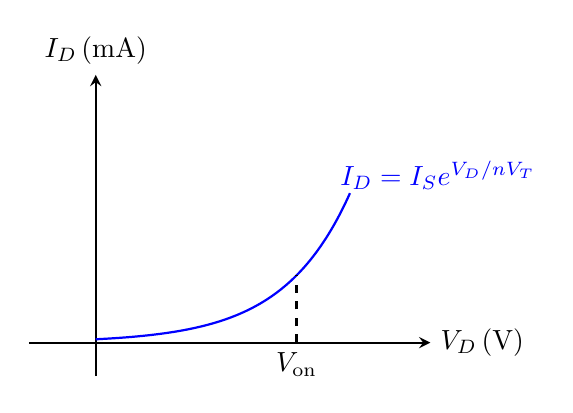
\begin{tikzpicture}[scale=0.85]
    \draw[->, >=stealth] (-1,0) -- (5,0) node[right] {$V_D\,\text{(V)}$};
    \draw[->, >=stealth] (0,-0.5) -- (0,4) node[above] {$I_D\,\text{(mA)}$};
    \draw[thick, color=blue, domain=0:3.8, samples=100] plot (\x, {0.05*exp(\x)});
    \node[color=blue, right] at (3.5,2.5) {$I_D = I_S e^{V_D/n V_T}$};
    \draw[dashed] (3,0) node[below] {$V_{\text{on}}$} -- (3,{0.05*exp(3)});
\end{tikzpicture}
\end{center}

\subsubsection*{Applications}
Highly precise analog designs, log/antilog amplifiers, temperature sensors, and computer-aided design (SPICE) simulations.

---

\subsection*{2. The Ideal Diode Model}

\subsubsection*{Theory and Circuit Operation}
The Ideal Diode Model is the simplest approximation, treating the diode as a perfect electronic switch. It assumes zero forward resistance and an instantaneous transition from non-conduction to conduction at a zero threshold voltage.

\subsubsection*{Mathematical Derivation}
The behavior is mathematically structured as a piecewise conditional state:
\begin{equation}
    \begin{cases} 
      V_D = 0, & \text{for } I_D > 0 \quad (\text{ON State / Short Circuit}) \\
      I_D = 0, & \text{for } V_D < 0 \quad (\text{OFF State / Open Circuit})
   \end{cases}
\end{equation}

\subsubsection*{Circuit Representation \& $i\text{-}v$ Curve}
\begin{center}
\begin{tabular}{cc}
\begin{circuitikz}[american, scale=0.8]
    \draw (0,1.5) to[D, l=$D$, v=$V_D$, i=$I_D$] (0,-1.5);
    \node at (1.5,0) {$\Longrightarrow$};
    \draw (3,1.5) to[switch, l=\text{Switch}] (3,-1.5);
\end{circuitikz} & 
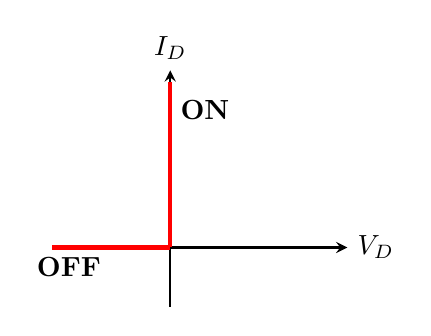
\begin{tikzpicture}[scale=0.75]
    \draw[->, >=stealth] (-2,0) -- (3,0) node[right] {$V_D$};
    \draw[->, >=stealth] (0,-1) -- (0,3) node[above] {$I_D$};
    \draw[ultra thick, color=red] (-2,0) -- (0,0);
    \draw[ultra thick, color=red] (0,0) -- (0,2.8);
    \node[anchor=south west] at (0,2) {\textbf{ON}};
    \node[anchor=north east] at (-1,0) {\textbf{OFF}};
\end{tikzpicture}
\end{tabular}
\end{center}

\subsubsection*{Applications}
Initial circuit inspection, high-voltage power supply rectification, and conceptual logic gate behavior analyses.

---

\subsection*{3. The Constant-Voltage-Drop (CVD) Model}

\subsubsection*{Theory and Circuit Operation}
The Constant-Voltage-Drop Model acknowledges that a semiconductor $p\text{-}n$ junction requires a specific potential barrier clearance to initiate conduction. Once the threshold voltage is reached, the diode conducts current with a fixed voltage drop, completely independent of the magnitude of the forward current.

\subsubsection*{Mathematical Derivation}
For silicon diodes, this stable threshold drop ($V_D$) is conventionally set to $0.7\,\text{V}$. The conditional state equation yields:
\begin{equation}
    \begin{cases} 
      V_D = 0.7\,\text{V}, & \text{for } I_D > 0 \quad (\text{ON State}) \\
      I_D = 0, & \text{for } V_D < 0.7\,\text{V} \quad (\text{OFF State})
   \end{cases}
\end{equation}

\subsubsection*{Circuit Representation \& $i\text{-}v$ Curve}
\begin{center}
\begin{tabular}{cc}
\begin{circuitikz}[american, scale=0.8]
    \draw (0,1.5) to[D, l=$D$, v=$V_D$, i=$I_D$] (0,-1.5);
    \node at (1.5,0) {$\Longrightarrow$};
    \draw (3,1.5) to[switch] (3,0.3) to[battery2, l=$0.7\,\text{V}$] (3,-1.5);
\end{circuitikz} & 
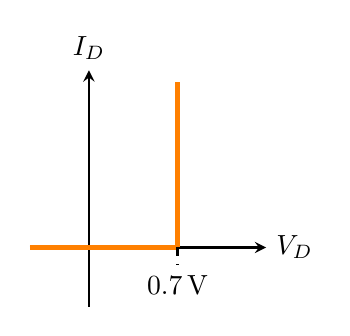
\begin{tikzpicture}[scale=0.75]
    \draw[->, >=stealth] (-1,0) -- (3,0) node[right] {$V_D$};
    \draw[->, >=stealth] (0,-1) -- (0,3) node[above] {$I_D$};
    \draw[ultra thick, color=orange] (-1,0) -- (1.5,0);
    \draw[ultra thick, color=orange] (1.5,0) -- (1.5,2.8);
    \draw[dashed] (1.5,0) -- (1.5,-0.3) node[below] {$0.7\,\text{V}$};
\end{tikzpicture}
\end{tabular}
\end{center}

\subsubsection*{Applications}
Standard analysis of typical analog circuits, power supply regulators, wave-shaping clippers, and clamping networks.

---

\subsection*{4. The Piecewise-Linear (PWL) Model}

\subsubsection*{Theory and Circuit Operation}
The Piecewise-Linear model scales up the CVD model by embedding an internal series dynamic resistance ($r_D$). This linearizes the slope of the forward exponential curve beyond the initial conduction threshold voltage ($V_{D0}$), matching the behavior of a real diode under varying current levels.

\subsubsection*{Mathematical Derivation}
When forward-biased beyond $V_{D0}$, the total forward voltage drop across the diode becomes linear with respect to the forward current:
\begin{equation}
    V_D = V_{D0} + I_D r_D \quad \text{for } V_D \ge V_{D0}
\end{equation}
The dynamic forward resistance is calculated mathematically as the inverse slope of the operational $i\text{-}v$ linear trace:
\begin{equation}
    r_D = \frac{\Delta V_D}{\Delta I_D} = \left. \frac{d v_D}{d i_D} \right|_{Q\text{-point}} = \frac{n V_T}{I_Q}
\end{equation}

\subsubsection*{Circuit Representation \& $i\text{-}v$ Curve}
\begin{center}
\begin{tabular}{cc}
\begin{circuitikz}[american, scale=0.8]
    \draw (0,1.5) to[D, l=$D$, v=$V_D$, i=$I_D$] (0,-1.5);
    \node at (1.5,0) {$\Longrightarrow$};
    \draw (3,1.5) to[switch] (3,0.5) to[battery2, l=$V_{D0}$] (3,-0.5) to[R, l=$r_D$] (3,-1.5);
\end{circuitikz} & 
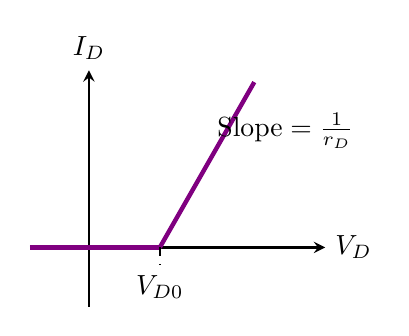
\begin{tikzpicture}[scale=0.75]
    \draw[->, >=stealth] (-1,0) -- (4,0) node[right] {$V_D$};
    \draw[->, >=stealth] (0,-1) -- (0,3) node[above] {$I_D$};
    \draw[ultra thick, color=violet] (-1,0) -- (1.2,0);
    \draw[ultra thick, color=violet] (1.2,0) -- (2.8,2.8);
    \draw[dashed] (1.2,0) -- (1.2,-0.3) node[below] {$V_{D0}$};
    \node[anchor=south west] at (2,1.5) {$\text{Slope} = \frac{1}{r_D}$};
\end{tikzpicture}
\end{tabular}
\end{center}

\subsubsection*{Applications}
Precise small-signal analysis, power electronics thermal estimations, and small-signal incremental amplifier architectures.

---

\subsection*{Summary and Comparison Model Table}

\begin{center}
\begin{tabularx}{\textwidth}{lXXXX}
\toprule
\textbf{Parameter} & \textbf{Exponential Model} & \textbf{Ideal Model} & \textbf{Constant-Voltage Drop} & \textbf{Piecewise-Linear} \\
\midrule
\textbf{Threshold ($V_{\text{on}}$)} & Variable ($I_D$ dependent) & $0\,\text{V}$ & $0.7\,\text{V}$ (Silicon) & $V_{D0} \approx 0.6\,\text{V} - 0.7\,\text{V}$ \\
\textbf{Internal Resistance} & Non-linear, dynamic & $0\,\Omega$ & $0\,\Omega$ & Finite dynamic $r_D$ \\
\textbf{Complexity Level} & Very High (Transcendental) & Extremely Low & Low & Moderate \\
\textbf{Accuracy Class} & Exact Physics Reference & First-Pass Approximation & Standard Practical Standard & High Local Linearity \\
\bottomrule
\end{tabularx}
\end{center}

\subsection*{Exam Tips}
\begin{itemize}
    \item When solving generic exam circuit problems, unless specified otherwise, default to the \textbf{Constant-Voltage-Drop Model} ($0.7\,\text{V}$ for Si) as it strikes the best balance between speed and practical accuracy.
    \item Always clarify your model assumption at the start of your calculation steps to secure full marks for method derivation.
\end{itemize}

\end{tcolorbox}

\item Determine the current $I_D$ and diode voltage $V_D$ for the circuit shown using:
\begin{enumerate}
  \item Piecewise linear model ($V_{DO}=0.7\,\text{V}$, $r_D=20\,\Omega$)
  \item Constant voltage drop model ($V_{DO}=0.7\,\text{V}$)
  \item Ideal diode model
\end{enumerate}
\begin{center}
\begin{circuitikz}[thick,american, thick, scale=1.2, transform shape]
  
  % Left branch (Battery)
  \draw (0,3) to[battery1, l=$5\text{V}$] (0,0);
  
  % Top branch (Horizontal Resistor)
  \draw (0,3) to[R, l_=$1\text{ k}\Omega$] (3,3);
  
  % Middle branch (Vertical Resistor)
  \draw (3,3) to[R, l_=$1\text{ k}\Omega$] (3,0);
  
  % Top wire to diode with current arrow
  \draw (3,3) to[short, i=$I_D$] (6,3);
  
  % Right branch (Diode)
  \draw (6,3) to[D] (6,0);
  
  % Bottom return wire
  \draw (0,0) -- (6,0);
  
  % Manual voltage labels across the diode
  \node at (6.5, 2.5) {$+$};
  \node at (6.6, 1.5) {$V_D$};
  \node at (6.5, 0.5) {$-$};
  
\end{circuitikz}
\end{center}

\mk{18} \yr{EEE 263 | L-2/T-1 | 2011--12}

\begin{tcolorbox}[enhanced,breakable,ansbox,colback=cA!4,colframe=cA,boxrule=0.8pt,arc=5pt,title={\textbf{Answer}},fonttitle=\bfseries\color{white},colbacktitle=cA]

\subsection*{1. Circuit Analysis and Th\'evenin Equivalent}

To determine the current $I_D$ and voltage $V_D$ across the diode efficiently for multiple models, we first simplify the linear portion of the circuit connected to the diode using Th\'evenin's theorem. 

\subsubsection*{Original Circuit}
\begin{center}
\begin{circuitikz}[american, thick, scale=1.0, transform shape]
  % Left branch (Battery)
  \draw (0,3) to[battery1, l=$5\,\text{V}$] (0,0);
  % Top branch (Horizontal Resistor)
  \draw (0,3) to[R, l=$1\,\text{k}\Omega$] (3,3);
  % Middle branch (Vertical Resistor)
  \draw (3,3) to[R, l=$1\,\text{k}\Omega$, *-*] (3,0);
  % Top wire to diode with current arrow
  \draw (3,3) to[short, i=$I_D$] (6,3);
  % Right branch (Diode)
  \draw (6,3) to[D] (6,0);
  % Bottom return wire
  \draw (0,0) -- (6,0);
  % Voltage labels across the diode
  \node at (6.5, 2.5) {$+$};
  \node at (6.6, 1.5) {$V_D$};
  \node at (6.5, 0.5) {$-$};
  % Ground
  \draw (3,0) node[ground] {};
\end{circuitikz}
\end{center}

\subsubsection*{Th\'evenin Simplification}
We remove the diode from the circuit to find the open-circuit Th\'evenin voltage ($V_{TH}$) and the Th\'evenin equivalent resistance ($R_{TH}$) looking back into the terminals.
\begin{align*}
    V_{TH} &= 5\,\text{V} \times \frac{1\,\text{k}\Omega}{1\,\text{k}\Omega + 1\,\text{k}\Omega} = 5\,\text{V} \times 0.5 = 2.5\,\text{V} \\
    R_{TH} &= 1\,\text{k}\Omega \parallel 1\,\text{k}\Omega = \frac{1\,\text{k}\Omega \times 1\,\text{k}\Omega}{1\,\text{k}\Omega + 1\,\text{k}\Omega} = 0.5\,\text{k}\Omega = 500\,\Omega
\end{align*}

Since $V_{TH} = 2.5\,\text{V}$ is strictly positive (and greater than typical diode turn-on voltages), we can safely assume the diode is \textbf{forward-biased (ON)} in all subsequent models. 

\begin{center}
\begin{circuitikz}[american, thick, scale=1.0, transform shape]
  % Thevenin Source
  \draw (0,3) to[V, l=$V_{TH}$, v_=$2.5\,\text{V}$] (0,0);
  % Thevenin Resistance
  \draw (0,3) to[R, l=$R_{TH}$, a_=$500\,\Omega$] (3,3);
  % Top wire to diode with current arrow
  \draw (3,3) to[short, i=$I_D$] (5,3);
  % Diode
  \draw (5,3) to[D] (5,0);
  % Bottom return wire
  \draw (0,0) -- (5,0);
  % Voltage labels across the diode
  \node at (5.5, 2.5) {$+$};
  \node at (5.6, 1.5) {$V_D$};
  \node at (5.5, 0.5) {$-$};
  \draw (0,0) node[ground] {};
\end{circuitikz}
\end{center}

---

\subsection*{2. Step-by-Step Solution for Diode Models}

\subsubsection*{(a) Piecewise Linear Model}
\textbf{Theory:} In the piecewise linear model, a forward-biased diode is replaced by a DC voltage source $V_{DO}$ in series with a dynamic forward resistance $r_D$. \\
Given: $V_{DO} = 0.7\,\text{V}$, $r_D = 20\,\Omega$.

Applying Kirchhoff's Voltage Law (KVL) to the Th\'evenin equivalent circuit:
\begin{align*}
    V_{TH} - I_D R_{TH} - V_{DO} - I_D r_D &= 0 \\
    I_D (R_{TH} + r_D) &= V_{TH} - V_{DO} \\
    I_D &= \frac{V_{TH} - V_{DO}}{R_{TH} + r_D}
\end{align*}
Substituting the values:
\begin{equation}
    I_D = \frac{2.5\,\text{V} - 0.7\,\text{V}}{500\,\Omega + 20\,\Omega} = \frac{1.8\,\text{V}}{520\,\Omega} \approx 3.4615\,\text{mA}
\end{equation}
The voltage across the diode $V_D$ is the sum of the threshold voltage and the drop across its internal resistance:
\begin{equation}
    V_D = V_{DO} + I_D r_D = 0.7\,\text{V} + (3.4615 \times 10^{-3}\,\text{A})(20\,\Omega) = 0.7\,\text{V} + 0.0692\,\text{V} = 0.7692\,\text{V}
\end{equation}

\subsubsection*{(b) Constant Voltage Drop Model}
\textbf{Theory:} This model assumes that once the diode is forward-biased, it maintains a constant voltage drop $V_{DO}$ regardless of the current flowing through it. It neglects the internal forward resistance ($r_D = 0$). \\
Given: $V_{DO} = 0.7\,\text{V}$.

Applying KVL:
\begin{equation}
    I_D = \frac{V_{TH} - V_{DO}}{R_{TH}}
\end{equation}
Substituting the values:
\begin{equation}
    I_D = \frac{2.5\,\text{V} - 0.7\,\text{V}}{500\,\Omega} = \frac{1.8\,\text{V}}{500\,\Omega} = 3.6\,\text{mA}
\end{equation}
The voltage across the diode is simply the constant threshold voltage:
\begin{equation}
    V_D = 0.7\,\text{V}
\end{equation}

\subsubsection*{(c) Ideal Diode Model}
\textbf{Theory:} The ideal diode model treats the forward-biased diode as a perfect conductor (short circuit) with zero voltage drop. \\
Given: $V_{DO} = 0\,\text{V}$, $r_D = 0\,\Omega$.

Applying KVL:
\begin{equation}
    I_D = \frac{V_{TH}}{R_{TH}}
\end{equation}
Substituting the values:
\begin{equation}
    I_D = \frac{2.5\,\text{V}}{500\,\Omega} = 5.0\,\text{mA}
\end{equation}
The voltage across the diode is zero:
\begin{equation}
    V_D = 0\,\text{V}
\end{equation}

---

\subsection*{3. Final Summary}

\begin{center}
\renewcommand{\arraystretch}{1.5}
\begin{tabular}{@{}llcc@{}}
\toprule
\textbf{Part} & \textbf{Diode Model} & \textbf{Diode Current ($I_D$)} & \textbf{Diode Voltage ($V_D$)} \\ \midrule
(a) & Piecewise Linear ($V_{DO}=0.7\,\text{V}, r_D=20\,\Omega$) & $3.46\,\text{mA}$ & $0.769\,\text{V}$ \\ 
(b) & Constant Voltage Drop ($V_{DO}=0.7\,\text{V}$) & $3.60\,\text{mA}$ & $0.700\,\text{V}$ \\ 
(c) & Ideal Diode & $5.00\,\text{mA}$ & $0.000\,\text{V}$ \\ \bottomrule
\end{tabular}
\end{center}

\end{tcolorbox}

\end{enumerate}

%%──────────────────────────────────────────────────────────────────────
\subtopic{cA}{Small Signal Model}
\label{sub:s1-ssm}

\begin{enumerate}
    
\item In the circuit shown, ``$I$'' is a DC current source and ``$V_i$'' is a sinusoidal signal with small amplitude ($<10\,\text{mV}$) and a frequency of 100\,kHz. Representing the diode by its small-signal resistance $r_d$ (a function of $I$):\\
(i) sketch the small-signal equivalent circuit for determining the sinusoidal output $V_o$ across the capacitor; \\ 
(ii) find the phase shift between $V_i$ and $V_o$; \\
(iii) find the value of $I$ that will provide a phase shift of $-45°$; \\
(iv) find the range of phase shift achieved as $I$ is varied from 0.1 to 10 times the value found in (iii). Assume $n=1$.\\
\begin{center}
        \begin{circuitikz}[american, thick]
        
        % Top Open Triangle Symbol
        \draw (0, 3) -- (0, 3.3);
        \draw (-0.15, 3.3) -- (0.15, 3.3) -- (0, 3.6) -- cycle;
        
        % Left Branch: Current Source -> Node -> Diode -> AC Source -> Ground
        \draw (0, 3) to[I, l=$I$, -*] (0, 1.5)
                     to[empty diode] (0, 0)
                     to[sV, l=$V_i$] (0, -1.5)
                     node[ground] {};
        
        % Right Branch: Connection -> Capacitor -> Ground
        \draw (0, 1.5) -- (2.5, 1.5)
                       to[C, l_=$10\,\text{nF}$] (2.5, 0)
                       -- (2.5, -0.5) node[ground] {};
        
        % Voltage Output Labels across Capacitor
        \node at (3.1, 1.2) {$+$};
        \node at (3.1, 0.75) {$V_o$};
        \node at (3.1, 0.3) {$-$};
        
    \end{circuitikz}
\end{center}
\mk{20} \yr{EEE 263 | L-2/T-1 | 2023--24}

\begin{tcolorbox}[enhanced,breakable,ansbox,colback=cA!4,colframe=cA,boxrule=0.8pt,arc=5pt,title={\textbf{Answer}},fonttitle=\bfseries\color{white},colbacktitle=cA]

\subsection*{Circuit Operation and Small-Signal Modeling}
The given circuit operates with a combination of a DC bias and a small-signal AC variation. 
\begin{itemize}
    \item \textbf{DC Analysis:} The ideal DC current source $I$ forces a constant bias current through the diode, establishing the quiescent operating point (Q-point). Because $V_i$ is a purely AC sinusoidal source, its DC voltage is $0\,\text{V}$ (acting as a short circuit to ground in DC analysis). Consequently, the entire DC current $I$ flows through the diode to ground.
    \item \textbf{AC Small-Signal Analysis:} By applying the superposition principle, the DC current source $I$ is deactivated (replaced by an open circuit because it is an ideal current source). The diode is replaced by its small-signal dynamic resistance $r_d$, which is determined by the DC bias current $I$.
\end{itemize}

\subsection*{(i) Small-Signal Equivalent Circuit}
To construct the small-signal equivalent circuit for determining the AC output $V_o$:
\begin{enumerate}
    \item The ideal DC current source $I$ becomes an open circuit.
    \item The diode is replaced by its small-signal resistance $r_d$.
    \item The rest of the AC components ($V_i$ and the $10\,\text{nF}$ capacitor) remain active.
\end{enumerate}

\begin{center}
\begin{circuitikz}[thick, american, scale=1.2, transform shape]
    % Left side AC Source
    \draw (0,0) to[sV, l=$V_i$] (0,2);
    % Resistor representing diode rd
    \draw (0,2) to[R, l=$r_d$, i=$i_d$] (3,2);
    % Output node and capacitor
    \draw (3,2) to[C, l_=$10\,\text{nF}$, *-] (3,0);
    % Ground line
    \draw (0,0) -- (4,0);
    \draw (2,0) node[ground] {};
    % Output voltage markers
    \node at (3.5, 1.8) {$+$}; 
    \node at (3.5, 1) {$V_o$}; 
    \node at (3.5, 0.2) {$-$};

\end{circuitikz}
\end{center}
\textit{Note: The circuit is drawn horizontally for standard signal flow. This electrically matches the vertical topology of the original circuit, forming a standard RC low-pass filter.}

---

\subsection*{(ii) Phase Shift between $V_i$ and $V_o$}
From the small-signal equivalent circuit, the system operates as an AC voltage divider. The output voltage $V_o$ is taken across the capacitor. Using complex impedances, the transfer function $H(j\omega)$ is:
\begin{align*}
    \frac{V_o}{V_i} &= \frac{Z_C}{r_d + Z_C} = \frac{\frac{1}{j\omega C}}{r_d + \frac{1}{j\omega C}} \\[8pt]
    \frac{V_o}{V_i} &= \frac{1}{1 + j\omega r_d C}
\end{align*}
The phase shift $\phi$ between the output $V_o$ and input $V_i$ is the phase angle of the transfer function:
\begin{align*}
    \phi &= \angle \left( \frac{1}{1 + j\omega r_d C} \right) = \angle(1) - \angle(1 + j\omega r_d C) \\[8pt]
    \phi &= 0^\circ - \tan^{-1}\left( \frac{\omega r_d C}{1} \right) \\[8pt]
    \phi &= -\tan^{-1}(\omega r_d C)
\end{align*}

---

\subsection*{(iii) Value of $I$ for a $-45^\circ$ Phase Shift}
We are given the required condition for the phase shift:
\begin{equation}
    \phi = -45^\circ
\end{equation}
Substituting this into our phase equation:
\begin{align*}
    -\tan^{-1}(\omega r_d C) &= -45^\circ \\[6pt]
    \omega r_d C &= \tan(45^\circ) = 1
\end{align*}
Solving for the required small-signal resistance $r_d$:
\begin{equation}
    r_d = \frac{1}{\omega C}
\end{equation}
Using the given parameters ($f = 100\,\text{kHz}$ and $C = 10\,\text{nF}$):
\begin{itemize}
    \item Angular frequency $\omega = 2\pi f = 2\pi \times 10^5\,\text{rad/s}$
    \item Capacitance $C = 10 \times 10^{-9}\,\text{F} = 10^{-8}\,\text{F}$
\end{itemize}
\begin{equation}
    r_d = \frac{1}{(2\pi \times 10^5)(10^{-8})} = \frac{1}{2\pi \times 10^{-3}} = \frac{500}{\pi}\,\Omega \approx 159.15\,\Omega
\end{equation}
The small-signal resistance of a diode is inversely proportional to its DC bias current:
\begin{equation}
    r_d = \frac{n V_T}{I} \implies I = \frac{n V_T}{r_d}
\end{equation}
Assuming a standard room temperature thermal voltage $V_T \approx 25\,\text{mV}$ and $n=1$ (given):
\begin{equation}
    I = \frac{1 \times 25 \times 10^{-3}\,\text{V}}{159.15\,\Omega} \approx 1.571 \times 10^{-4}\,\text{A} = \mathbf{157.1\,\mu\text{A}}
\end{equation}

---

\subsection*{(iv) Range of Phase Shift as $I$ is Varied}
Let $I_{45}$ be the current found in part (iii) that yields $\omega r_d C = 1$. Because $r_d = \frac{n V_T}{I}$, the resistance $r_d$ scales inversely with $I$. Consequently, the unitless product $\omega r_d C$ also scales inversely with $I$:
\begin{equation}
    \omega r_d C = \frac{I_{45}}{I}
\end{equation}
We evaluate the phase shift $\phi = -\tan^{-1}(\omega r_d C)$ at the two extremes of the given current range:

\begin{enumerate}
    \item \textbf{When $I = 0.1 \times I_{45}$:} 
    \begin{equation}
        \omega r_d C = \frac{I_{45}}{0.1 I_{45}} = 10
    \end{equation}
    \begin{equation}
        \phi_1 = -\tan^{-1}(10) \approx \mathbf{-84.29^\circ}
    \end{equation}
    
    \item \textbf{When $I = 10 \times I_{45}$:} 
    \begin{equation}
        \omega r_d C = \frac{I_{45}}{10 I_{45}} = 0.1
    \end{equation}
    \begin{equation}
        \phi_2 = -\tan^{-1}(0.1) \approx \mathbf{-5.71^\circ}
    \end{equation}
\end{enumerate}

\textbf{Final Conclusion:} By varying the DC bias current $I$ from 0.1 to 10 times the center $-45^\circ$ condition value, the phase shift can be electronically tuned over a range from \textbf{$-5.71^\circ$ to $-84.29^\circ$}. This highlights the circuit's fundamental utility as a highly tunable current-controlled phase shifter.

\end{tcolorbox}

\item The small-signal model of a diode is said to be valid for voltage variations of about 10\,mV. To what percentage current change does this correspond for $n=1$ (consider both positive and negative signals)? What is the maximum allowable voltage signal (positive or negative) if the current change is limited to 10\%?
\mk{10} \yr{EEE 263 | L-2/T-1 | 2014--15}

\begin{tcolorbox}[enhanced,breakable,ansbox,colback=cA!4,colframe=cA,boxrule=0.8pt,arc=5pt,title={\textbf{Answer}},fonttitle=\bfseries\color{white},colbacktitle=cA]

\subsection*{Theory: Diode Large-Signal and Small-Signal Analysis}

The total instantaneous current $i_D$ flowing through a forward-biased diode is related to the total instantaneous voltage $v_D$ across it by the exact exponential equation:
\begin{equation}
    i_D = I_S e^{\frac{v_D}{n V_T}}
\end{equation}

In a small-signal application, the diode operates at a DC quiescent point (Q-point) defined by a DC voltage $V_D$ and a corresponding DC current $I_D$, upon which a small time-varying AC signal $v_d$ is superimposed:
\begin{equation}
    v_D(t) = V_D + v_d(t)
\end{equation}

Substituting this into the diode equation yields the total instantaneous current:
\begin{equation}
    i_D = I_S e^{\frac{V_D + v_d}{n V_T}} = \left( I_S e^{\frac{V_D}{n V_T}} \right) e^{\frac{v_d}{n V_T}} = I_D e^{\frac{v_d}{n V_T}}
\end{equation}

The change in the diode current, $\Delta i$, due to the AC signal $v_d$ is:
\begin{equation}
    \Delta i = i_D - I_D = I_D \left( e^{\frac{v_d}{n V_T}} - 1 \right)
\end{equation}

The \textbf{fractional (or percentage) current change} is thus defined as:
\begin{equation}
    \frac{\Delta i}{I_D} = e^{\frac{v_d}{n V_T}} - 1
    \label{eq:fractional_change}
\end{equation}

\textit{Assumption:} For typical small-signal analysis at room temperature, the thermal voltage is assumed to be $V_T \approx 25\,\text{mV}$. The ideality factor is given as $n=1$.

---

\subsection*{Part 1: Percentage Current Change for $v_d = \pm 10\,\text{mV}$}

To evaluate the validity of the small-signal approximation for a $\pm 10\,\text{mV}$ variation, we use Equation \eqref{eq:fractional_change}. 

\textbf{Case 1A: Positive Voltage Signal ($v_d = +10\,\text{mV}$)}
\begin{align*}
    \frac{\Delta i}{I_D} &= e^{\frac{+10\,\text{mV}}{1 \times 25\,\text{mV}}} - 1 \\
    &= e^{0.4} - 1 \\
    &\approx 1.4918 - 1 = 0.4918
\end{align*}
Expressed as a percentage, a $+10\,\text{mV}$ variation causes a \textbf{$+49.2\%$} increase in current.

\textbf{Case 1B: Negative Voltage Signal ($v_d = -10\,\text{mV}$)}
\begin{align*}
    \frac{\Delta i}{I_D} &= e^{\frac{-10\,\text{mV}}{1 \times 25\,\text{mV}}} - 1 \\
    &= e^{-0.4} - 1 \\
    &\approx 0.6703 - 1 = -0.3297
\end{align*}
Expressed as a percentage, a $-10\,\text{mV}$ variation causes a \textbf{$-33.0\%$} decrease in current.

\textit{Important Note:} The asymmetry ($+49.2\%$ vs. $-33.0\%$) arises directly from the highly non-linear (exponential) nature of the diode's $i-v$ characteristic. The small-signal (linear) model predicts a symmetric $\pm 40\%$ change ($\frac{v_d}{V_T} = \frac{10}{25}$), illustrating the approximation error when $v_d$ is as large as $10\,\text{mV}$.

---

\subsection*{Part 2: Maximum Voltage Signal for a 10\% Current Change}

To ensure high linearity, we often restrict the current change to $\pm 10\%$. We must find the maximum allowable voltage signal $v_d$ that satisfies this constraint.

Rearranging Equation \eqref{eq:fractional_change} to solve for $v_d$:
\begin{equation}
    v_d = n V_T \ln \left( 1 + \frac{\Delta i}{I_D} \right)
\end{equation}

\textbf{Case 2A: Positive Current Limit ($\frac{\Delta i}{I_D} = +0.10$)}
\begin{align*}
    v_{d(\text{max}+)} &= 1 \times 25\,\text{mV} \times \ln(1 + 0.10) \\
    &= 25\,\text{mV} \times \ln(1.10) \\
    &\approx 25\,\text{mV} \times 0.0953 \\
    &= \mathbf{+2.38\,\text{mV}}
\end{align*}

\textbf{Case 2B: Negative Current Limit ($\frac{\Delta i}{I_D} = -0.10$)}
\begin{align*}
    v_{d(\text{max}-)} &= 1 \times 25\,\text{mV} \times \ln(1 - 0.10) \\
    &= 25\,\text{mV} \times \ln(0.90) \\
    &\approx 25\,\text{mV} \times (-0.1054) \\
    &= \mathbf{-2.63\,\text{mV}}
\end{align*}

---

\subsection*{Final Answer Summary}

\begin{center}
\renewcommand{\arraystretch}{1.5}
\begin{tabular}{@{}ll@{}}
\toprule
\textbf{Parameter} & \textbf{Calculated Value} \\ \midrule
Percentage Current Change for $v_d = +10\,\text{mV}$ & $\mathbf{+49.2\%}$ \\
Percentage Current Change for $v_d = -10\,\text{mV}$ & $\mathbf{-33.0\%}$ \\
Maximum Positive Voltage Signal for $+10\%$ Current Change & $\mathbf{+2.38\,\text{mV}}$ \\
Maximum Negative Voltage Signal for $-10\%$ Current Change & $\mathbf{-2.63\,\text{mV}}$ \\ \bottomrule
\end{tabular}
\end{center}

\textbf{Exam Tip:} Notice that to keep the small-signal model highly accurate (within 10\% distortion), the AC voltage signal amplitude must be kept very small—generally strictly less than roughly $2.5\,\text{mV}$ for $n=1$.

\end{tcolorbox}

\end{enumerate}

%%──────────────────────────────────────────────────────────────────────
\subtopic{cA}{Peak Rectifier}
\label{sub:s1-peak}

\begin{enumerate}
    
\item Consider a half-wave rectifier circuit with $R=1\,\text{k}\Omega$ load operating from a 120\,V (rms), 60\,Hz household supply through a 10-to-1 step-down transformer, augmented with a filter capacitor $C$ across the load. Assume $V_D=0.7\,\text{V}$ for any current. \\
(i) Find $C$ for a peak-to-peak ripple of 10\% of peak output.\\
 (ii) Find $C$ for a peak-to-peak ripple of 1\% of peak output. \\
 (iii) Find the average output voltage for each of the case (i) \& (ii) . \\
 (iv) Find the fraction of the cycle for which the diode conducts for each of the case (i) \& (ii).\\
 (v) Find the average and peak diode currents for each of the case (i) \& (ii).\\
\mk{20} \yr{EEE 263 | L-2/T-1 | 2024--25}

\begin{tcolorbox}[enhanced,breakable,ansbox,colback=cA!4,colframe=cA,boxrule=0.8pt,arc=5pt,title={\textbf{Answer}},fonttitle=\bfseries\color{white},colbacktitle=cA]

\subsection*{Circuit Diagram}
\begin{center}
\begin{circuitikz}[american, x=1.4cm, thick, scale=1.0, transform shape]
    % Source
    \draw (0,0) to[sV, l={$120\,\text{V}_{\text{rms}}, 60\,\text{Hz}$}] (0,4) -- (1.5,4);
    % Primary Coil
    \draw (1.5,4) to[L, l_=$N_1$] (1.5,0) -- (0,0);
    % Core
    \draw[ultra thick] (1.8,0.5) -- (1.8,3.5);
    \draw[ultra thick] (2.0,0.5) -- (2.0,3.5);
    % Secondary Coil
    \draw (2.3,4) to[L, l=$N_2$] (2.3,0);
    % Turns ratio label
    \node at (1.9, 4.3) {$10:1$};
    % Diode
    \draw (2.3,4) to[D, l=$D$, v=$0.7\,\text{V}$, -*] (5,4);
    % Capacitor & Load
    \draw (5,4) to[C, l_=$C$, *-*] (5,0);
    \draw (5,4) -- (7,4) to[R, l_={$R=1\,\text{k}\Omega$}] (7,0);
    % Return path
    \draw (2.3,0) -- (7,0);
    \draw (5,0) node[ground]{};
    % Output label
    \node at (7.5, 3.8) {$+$};
    \node at (7.5, 2) {$V_o$};
    \node at (7.5, 0.2) {$-$};
\end{circuitikz}
\end{center}


\subsection*{Theory \& Initial Calculations}

\textbf{1. Secondary Voltage Calculation:}
The step-down transformer reduces the primary AC voltage by the turns ratio $N_1/N_2 = 10$.
\begin{equation}
    V_{s(\text{rms})} = \frac{V_{p(\text{rms})}}{10} = \frac{120\,\text{V}}{10} = 12\,\text{V}_{\text{rms}}
\end{equation}
The peak voltage of the secondary transformer winding is:
\begin{equation}
    V_{s(\text{peak})} = V_{s(\text{rms})} \times \sqrt{2} = 12\sqrt{2} \approx 16.97\,\text{V}
\end{equation}

\textbf{2. Peak Output Voltage ($V_p$):}
For a half-wave rectifier, the diode conducts when forward-biased, causing a constant voltage drop $V_D = 0.7\,\text{V}$. The peak output voltage across the load and capacitor is:
\begin{equation}
    V_p = V_{s(\text{peak})} - V_D = 16.97\,\text{V} - 0.7\,\text{V} = 16.27\,\text{V}
\end{equation}
\textit{Note: The ripple frequency $f$ for a half-wave rectifier is equal to the source frequency ($60\,\text{Hz}$).}

---

\subsection*{Step-by-Step Solution}

We utilize the standard approximations for peak rectifier circuits (valid when $V_r \ll V_p$):
\begin{itemize}
    \item \textbf{Ripple Voltage:} $V_r \approx \frac{V_p}{f R C}$
    \item \textbf{DC Output Voltage:} $V_{\text{dc}} \approx V_p - \frac{V_r}{2}$
    \item \textbf{Conduction Angle:} $\theta_c = \omega \Delta t \approx \sqrt{\frac{2 V_r}{V_p}} \text{ (in radians)}$
    \item \textbf{Average Diode Current (Full Cycle):} $I_{D,\text{avg}} = I_{\text{load}} = \frac{V_{\text{dc}}}{R}$
    \item \textbf{Peak Diode Current:} $i_{D,\text{max}} = I_{\text{load}} \left( 1 + 2\pi \sqrt{\frac{2 V_p}{V_r}} \right)$
\end{itemize}

\subsubsection*{Case (i): Peak-to-Peak Ripple is 10\% of Peak Output}

Given $V_r = 0.10 \times V_p = 0.10 \times 16.27\,\text{V} = 1.627\,\text{V}$.

\textbf{(i) Filter Capacitor $C$:}
\begin{equation}
    C = \frac{V_p}{V_r f R} = \frac{V_p}{0.10 V_p f R} = \frac{1}{0.10 \times 60 \times 1000} = \frac{1}{6000} \approx \mathbf{166.7\,\mu\text{F}}
\end{equation}

\textbf{(iii) Average Output Voltage ($V_{\text{dc}}$):}
\begin{equation}
    V_{\text{dc}} = V_p - \frac{V_r}{2} = 16.27 - \frac{1.627}{2} = 16.27 - 0.8135 = \mathbf{15.46\,\text{V}}
\end{equation}

\textbf{(iv) Fraction of Cycle for Conduction:}
The conduction angle $\theta_c = \sqrt{\frac{2 \times 0.10 V_p}{V_p}} = \sqrt{0.20} \approx 0.4472\,\text{rad}$.
\begin{equation}
    \text{Fraction} = \frac{\theta_c}{2\pi} = \frac{0.4472}{2\pi} \approx \mathbf{0.0712} \text{ (or } 7.12\%)
\end{equation}

\textbf{(v) Average and Peak Diode Currents:}
The average diode current over the entire cycle equals the DC load current:
\begin{equation}
    I_{D,\text{avg}} = I_{\text{load}} = \frac{V_{\text{dc}}}{R} = \frac{15.46\,\text{V}}{1\,\text{k}\Omega} = \mathbf{15.46\,\text{mA}}
\end{equation}
The peak diode current is calculated as:
\begin{equation}
    i_{D,\text{max}} = I_{\text{load}} \left( 1 + 2\pi \sqrt{\frac{2 V_p}{0.10 V_p}} \right) = 15.46\,\text{mA} \left( 1 + 2\pi \sqrt{20} \right) \approx 15.46 (1 + 28.10) = \mathbf{449.8\,\text{mA}}
\end{equation}

---

\subsubsection*{Case (ii): Peak-to-Peak Ripple is 1\% of Peak Output}

Given $V_r = 0.01 \times V_p = 0.01 \times 16.27\,\text{V} = 0.1627\,\text{V}$.

\textbf{(ii) Filter Capacitor $C$:}
\begin{equation}
    C = \frac{V_p}{V_r f R} = \frac{1}{0.01 \times 60 \times 1000} = \frac{1}{600} \approx \mathbf{1666.7\,\mu\text{F}} \text{ (or } 1.67\,\text{mF)}
\end{equation}

\textbf{(iii) Average Output Voltage ($V_{\text{dc}}$):}
\begin{equation}
    V_{\text{dc}} = V_p - \frac{V_r}{2} = 16.27 - \frac{0.1627}{2} = 16.27 - 0.08135 = \mathbf{16.19\,\text{V}}
\end{equation}

\textbf{(iv) Fraction of Cycle for Conduction:}
The conduction angle $\theta_c = \sqrt{\frac{2 \times 0.01 V_p}{V_p}} = \sqrt{0.02} \approx 0.1414\,\text{rad}$.
\begin{equation}
    \text{Fraction} = \frac{\theta_c}{2\pi} = \frac{0.1414}{2\pi} \approx \mathbf{0.0225} \text{ (or } 2.25\%)
\end{equation}

\textbf{(v) Average and Peak Diode Currents:}
The average diode current over the entire cycle:
\begin{equation}
    I_{D,\text{avg}} = I_{\text{load}} = \frac{V_{\text{dc}}}{R} = \frac{16.19\,\text{V}}{1\,\text{k}\Omega} = \mathbf{16.19\,\text{mA}}
\end{equation}
The peak diode current is:
\begin{equation}
    i_{D,\text{max}} = 16.19\,\text{mA} \left( 1 + 2\pi \sqrt{\frac{2 V_p}{0.01 V_p}} \right) = 16.19\,\text{mA} \left( 1 + 2\pi \sqrt{200} \right) \approx 16.19 (1 + 88.86) = \mathbf{1454.8\,\text{mA}} \text{ (or } 1.45\,\text{A)}
\end{equation}

---

\subsection*{Final Answer Summary Table}
\begin{center}
\renewcommand{\arraystretch}{1.4}
\begin{tabular}{@{}llcc@{}}
\toprule
\textbf{Part} & \textbf{Parameter} & \textbf{Case (i) 10\% Ripple} & \textbf{Case (ii) 1\% Ripple} \\ \midrule
(i), (ii) & Filter Capacitor ($C$) & $166.7\,\mu\text{F}$ & $1666.7\,\mu\text{F}$ \\ 
(iii) & Average Output Voltage ($V_{\text{dc}}$) & $15.46\,\text{V}$ & $16.19\,\text{V}$ \\ 
(iv) & Conduction Fraction & $0.0712$ ($7.12\%$) & $0.0225$ ($2.25\%$) \\ 
(v) & Cycle-Average Diode Current ($I_{D,\text{avg}}$) & $15.46\,\text{mA}$ & $16.19\,\text{mA}$ \\ 
(v) & Peak Diode Current ($i_{D,\text{max}}$) & $449.8\,\text{mA}$ & $1454.8\,\text{mA}$ \\ 
\bottomrule
\end{tabular}
\end{center}

\textbf{Important Note on Diode Current:} 
The $I_{D,\text{avg}}$ computed above is the average over the \textit{entire cycle}, corresponding to the DC load current $I_{\text{load}}$. If a question explicitly asks for the average current strictly \textit{during the conduction interval}, it is calculated as $I_{D(\text{cond\_avg})} = I_{\text{load}} / \text{Fraction}$.

\end{tcolorbox}

\item Consider a peak rectifier fed by a 60\,Hz sinusoid with a peak value $V_p=100\,\text{V}$. Let the load resistance $R=10\,\text{k}\Omega$. Find the value of capacitance $C$ that will result in a peak-to-peak ripple of 2\,V. Also calculate the fraction of the cycle during which the diode is conducting and the average and peak values of the diode current.
\mk{10} \yr{EEE 263 | L-2/T-1 | 2017--18}

\begin{tcolorbox}[enhanced,breakable,ansbox,colback=cA!4,colframe=cA,boxrule=0.8pt,arc=5pt,title={\textbf{Answer}},fonttitle=\bfseries\color{white},colbacktitle=cA]

\textbf{Assumptions:} \\
For this analysis, we assume an ideal diode model ($V_{D,on} = 0\,\text{V}$) since the peak input voltage ($V_p = 100\,\text{V}$) is significantly larger than the typical forward voltage drop of a practical diode. Furthermore, since the specified ripple ($2\,\text{V}$) is very small compared to the peak voltage ($V_r \ll V_p$), the standard small-ripple textbook approximations hold true.

\subsubsection*{Circuit Diagram: Half-Wave Peak Rectifier}
\begin{center}
\begin{circuitikz}[american,thick,  scale=1.1, transform shape]
    % AC Source
    \draw (0,0) to[sV, l={$v_s(t)=V_p\sin(\omega t)$}] (0,3);
    % Diode
    \draw (0,3) to[D, l=$D$, i=$i_D(t)$] (3,3);
    % Top and Bottom Rails
    \draw (3,3) -- (6,3);
    \draw (0,0) -- (6,0);
    % Filter Capacitor
    \draw (3,3) to[C, l=$C$, v=$v_o(t)$] (3,0);
    % Load Resistor
    \draw (6,3) to[R, l=$R$, i=$I_L$] (6,0);
    % Ground Connection
    \draw (3,0) node[ground]{};
    % Output Node Label
    \node[above] at (4.5,3) {$V_{out}$};
\end{circuitikz}
\end{center}

\subsubsection*{Given Parameters}
\begin{itemize}
    \item Source frequency, $f = 60\,\text{Hz}$
    \item Peak input voltage, $V_p = 100\,\text{V}$
    \item Load resistance, $R = 10\,\text{k}\Omega$
    \item Peak-to-peak ripple voltage, $V_r = 2\,\text{V}$
\end{itemize}

\vspace{0.5em}
 
\vspace{0.5em}

\subsubsection*{1. Calculation of Filter Capacitance ($C$)}
In a peak rectifier with a small ripple, the capacitor discharges linearly through the load resistor $R$ over approximately the entire period $T \approx \frac{1}{f}$. The peak-to-peak ripple voltage $V_r$ is given by:
\begin{equation*}
    V_r \approx \frac{V_p}{f R C}
\end{equation*}
Rearranging to solve for the capacitance $C$:
\begin{align*}
    C &= \frac{V_p}{f R V_r} \\
    &= \frac{100}{60 \times (10 \times 10^3) \times 2} \\
    &= \frac{100}{1.2 \times 10^6} \approx 83.33 \times 10^{-6}\,\text{F} = \mathbf{83.33\,\mu\text{F}}
\end{align*}

\subsubsection*{2. Conduction Angle and Fraction of the Cycle}
The diode only conducts during a short interval $\Delta t$ near the peak of the input voltage to replenish the charge lost by the capacitor. The conduction angle $\theta_c = \omega \Delta t$ can be approximated by:
\begin{equation*}
    \omega \Delta t \approx \sqrt{\frac{2V_r}{V_p}}
\end{equation*}
Substituting the known values:
\begin{align*}
    \omega \Delta t &= \sqrt{\frac{2 \times 2}{100}} = \sqrt{0.04} = \mathbf{0.2\,\text{rad}}
\end{align*}
To find the fraction of the cycle during which the diode conducts, we divide the conduction angle by a full period ($2\pi$ radians):
\begin{align*}
    \text{Fraction} &= \frac{\omega \Delta t}{2\pi} = \frac{0.2}{2\pi} \approx \mathbf{0.0318 \text{ (or } 3.18\%)}
\end{align*}

\subsubsection*{3. Average and Peak Diode Currents}
During the non-conduction interval, the load current $I_L$ is approximately constant and is supplied entirely by the capacitor:
\begin{equation*}
    I_L \approx \frac{V_p}{R} = \frac{100}{10\,\text{k}\Omega} = 10\,\text{mA}
\end{equation*}

\textbf{Average Diode Current ($i_{D,avg}$):} \\
To maintain steady-state, the charge supplied by the diode during the short conduction interval must equal the charge drawn by the load over the full cycle. The average diode current during conduction is derived as:
\begin{align*}
    i_{D,avg} &= I_L \left( 1 + \pi \sqrt{\frac{2V_p}{V_r}} \right) \\
    &= 10\,\text{mA} \left( 1 + \pi \sqrt{\frac{2 \times 100}{2}} \right) \\
    &= 10\,\text{mA} \left( 1 + 10\pi \right) \\
    &\approx 10\,\text{mA} \times (1 + 31.416) = \mathbf{324.16\,\text{mA}}
\end{align*}

\textbf{Peak Diode Current ($i_{D,max}$):} \\
The maximum diode current occurs at the beginning of the conduction interval and is approximately twice the average charging current plus the load current:
\begin{align*}
    i_{D,max} &= I_L \left( 1 + 2\pi \sqrt{\frac{2V_p}{V_r}} \right) \\
    &= 10\,\text{mA} \left( 1 + 2\pi \sqrt{\frac{2 \times 100}{2}} \right) \\
    &= 10\,\text{mA} \left( 1 + 20\pi \right) \\
    &\approx 10\,\text{mA} \times (1 + 62.832) = \mathbf{638.32\,\text{mA}}
\end{align*}

\vspace{0.5em}
 
\vspace{0.5em}

\subsubsection*{Final Answer Summary}
\begin{center}
\renewcommand{\arraystretch}{1.5}
\begin{tabular}{@{}ll@{}}
    \toprule
    \textbf{Parameter} & \textbf{Calculated Value} \\
    \midrule
    Filter Capacitance ($C$) & $83.33\,\mu\text{F}$ \\
    Conduction Angle ($\omega \Delta t$) & $0.2\,\text{rad}$ \\
    Conduction Fraction & $3.18\%$ \\
    Average Diode Current ($i_{D,avg}$) & $324.16\,\text{mA}$ \\
    Peak Diode Current ($i_{D,max}$) & $638.32\,\text{mA}$ \\
    \bottomrule
\end{tabular}
\end{center}

\end{tcolorbox}

\item Consider a half-wave peak rectifier fed with a voltage having a triangular waveform with 20\,V peak-to-peak amplitude, zero average and 1\,kHz frequency. Load resistance $R=100\,\Omega$ and filter capacitor $C=100\,\mu$F. Assume the diode has a forward voltage drop of 0.7\,V when conducting. Find: (i) average DC output voltage, (ii) time interval during which the diode conducts, (iii) average diode current during conduction, (iv) maximum diode current.
\mk{20} \yr{EEE 263 | L-2/T-1 | 2016--17}

\begin{tcolorbox}[enhanced,breakable,ansbox,colback=cA!4,colframe=cA,boxrule=0.8pt,arc=5pt,title={\textbf{Answer}},fonttitle=\bfseries\color{white},colbacktitle=cA]

\subsubsection*{Theory and Circuit Operation}
A peak rectifier (or envelope detector) consists of a diode and a filter capacitor connected in parallel with a load resistance. When a zero-average triangular waveform is applied:
\begin{enumerate}
    \item \textbf{Conduction Phase:} On the rising edge of the input voltage $v_s(t)$, once it exceeds the capacitor voltage plus the diode forward drop ($v_s > v_o + V_D$), the diode turns ON. The capacitor quickly charges up, following the input waveform minus the diode drop: $v_o(t) = v_s(t) - V_D$.
    \item \textbf{Non-Conduction Phase:} Immediately after the input passes its peak, the input slope decreases rapidly. The diode turns OFF because the capacitor cannot discharge fast enough to follow the sharp drop of the triangular input. The capacitor then discharges exponentially through the load resistor $R$ with a time constant $\tau = RC$.
\end{enumerate}

\subsubsection*{Circuit Diagram}
\begin{center}
\begin{circuitikz}[american, thick, scale=1.1, transform shape]
    % Source
    \draw (0,3) to[V, l_=$v_s(t)$] (0,0);
    % Diode
    \draw (0,3) to[D, l=$D$, v=$V_D$, i=$i_D(t)$] (3,3);
    % Rails
    \draw (3,3) -- (6,3);
    \draw (0,0) -- (6,0);
    % Capacitor
    \draw (3,3) to[C, l=$C$, v=$v_o(t)$] (3,0);
    % Resistor
    \draw (6,3) to[R, l=$R$, i=$i_L(t)$] (6,0);
    % Ground
    \draw (3,0) node[ground]{};
    % Node Label
    \node[above] at (4.5,3) {$V_{out}$};
\end{circuitikz}
\end{center}

\subsubsection*{Given Parameters}
\begin{itemize}
    \item Peak-to-peak input voltage: $V_{pp} = 20\,\text{V}$
    \item Zero-average input implies: Peak input voltage $V_p = \frac{V_{pp}}{2} = 10\,\text{V}$
    \item Input frequency: $f = 1\,\text{kHz} \implies \text{Period } T = \frac{1}{f} = 1\,\text{ms}$
    \item Load resistance: $R = 100\,\Omega$
    \item Filter capacitance: $C = 100\,\mu\text{F}$
    \item Diode forward voltage drop: $V_D = 0.7\,\text{V}$
\end{itemize}

The discharge time constant is:
\begin{equation*}
    \tau = RC = 100\,\Omega \times 100\,\mu\text{F} = 10\,\text{ms}
\end{equation*}
Since $\tau = 10\,\text{ms} \gg T = 1\,\text{ms}$, the small-ripple approximation and linear discharge assumption are highly accurate.

\vspace{0.5em}
 
\vspace{0.5em}

\subsubsection*{Mathematical Derivation and Step-by-Step Solution}

The maximum output voltage reached at the peak of the input is:
\begin{equation*}
    V_{omax} = V_p - V_D = 10\,\text{V} - 0.7\,\text{V} = 9.3\,\text{V}
\end{equation*}

\paragraph{(i) Calculation of Peak-to-Peak Ripple ($V_r$) and Average DC Output Voltage ($V_{out,avg}$)}
During the non-conduction phase, which lasts for approximately the entire period ($T - \Delta t \approx T$), the capacitor discharges linearly. The peak-to-peak ripple voltage $V_r$ can be expressed as:
\begin{equation}
    V_r \approx \frac{V_{omax}}{RC}(T - \Delta t)
\end{equation}

On the rising edge of the triangular wave leading up to the peak (defined at $t=0$), the slope of the input voltage is constant:
\begin{equation*}
    \frac{dv_s}{dt} = \frac{V_{pp}}{T/2} = \frac{20\,\text{V}}{0.5\,\text{ms}} = 40,000\,\text{V/s} = 40\,\text{V/ms}
\end{equation*}

The diode turns ON at a time $t = -\Delta t$ before the peak, where the input voltage rises enough to forward-bias the diode:
\begin{equation*}
    V_r = \left(\frac{dv_s}{dt}\right) \Delta t = 40,000 \cdot \Delta t
\end{equation*}

Equating the two relationships for $V_r$ (using millisecond units for simplicity):
\begin{align*}
    40 \cdot \Delta t &= \frac{9.3}{10} (1 - \Delta t) \\
    40 \cdot \Delta t &= 0.93 - 0.93 \cdot \Delta t \\
    40.93 \cdot \Delta t &= 0.93 \implies \Delta t = \frac{0.93}{40.93} \approx \mathbf{0.02272\,\text{ms} = 22.72\,\mu\text{s}}
\end{align*}

Now, substituting $\Delta t$ back to find the precise ripple voltage $V_r$:
\begin{equation*}
    V_r = 40\,\text{V/ms} \times 0.02272\,\text{ms} = 0.9089\,\text{V}
\end{equation*}

The average DC output voltage is the midpoint of the linear ripple waveform:
\begin{align*}
    V_{out,avg} &= V_{omax} - \frac{V_r}{2} \\
    &= 9.3\,\text{V} - \frac{0.9089\,\text{V}}{2} = 9.3\,\text{V} - 0.4545\,\text{V} = \mathbf{8.8455\,\text{V}}
\end{align*}

\paragraph{(ii) Time Interval During Which the Diode Conducts ($\Delta t$)}
As derived above during the simultaneous solution for the ripple voltage:
\begin{equation*}
    \Delta t = \mathbf{22.72\,\mu\text{s}}
\end{equation*}

\paragraph{(iii) Average Diode Current During Conduction ($i_{D,avg}$)}
During the conduction interval $\Delta t$, the diode current $i_D(t)$ splits into the capacitor charging current $i_C(t)$ and the load current $i_L(t)$:
\begin{equation*}
    i_D(t) = i_C(t) + i_L(t) = C\frac{dv_o}{dt} + \frac{v_o(t)}{R}
\end{equation*}

Since $v_o(t) = v_s(t) - V_D$ during conduction, its slope matches the input slope:
\begin{equation*}
    i_C(t) = C\frac{dv_s}{dt} = 100\,\mu\text{F} \times 40,000\,\text{V/s} = 4.0\,\text{A} \quad (\text{constant during conduction})
\end{equation*}

The average load current during this short conduction window is determined by the average output voltage during conduction, which matches $V_{out,avg}$:
\begin{equation*}
    i_{L,avg} = \frac{V_{out,avg}}{R} = \frac{8.8455\,\text{V}}{100\,\Omega} = 0.08846\,\text{A} = 88.46\,\text{mA}
\end{equation*}

Thus, the total average current flowing through the diode *during the conduction interval* is:
\begin{align*}
    i_{D,avg} &= i_C + i_{L,avg} \\
    &= 4.0\,\text{A} + 0.08846\,\text{A} = \mathbf{4.0885\,\text{A}}
\end{align*}

\paragraph{(iv) Maximum Diode Current ($i_{D,max}$)}
The maximum diode current occurs exactly at the peak of the input ($t = 0$), where the output voltage reaches its maximum value $V_{omax} = 9.3\,\text{V}$:
\begin{align*}
    i_{D,max} &= i_C + i_{L,max} \\
    &= C\frac{dv_o}{dt} + \frac{V_{omax}}{R} \\
    &= 4.0\,\text{A} + \frac{9.3\,\text{V}}{100\,\Omega} = 4.0\,\text{A} + 0.093\,\text{A} = \mathbf{4.093\,\text{A}}
\end{align*}

\vspace{0.5em}
 
\vspace{0.5em}

\subsubsection*{Final Answer Summary}
\begin{center}
\renewcommand{\arraystretch}{1.5}
\begin{tabular}{@{}lll@{\quad}l@{}}
    \toprule
    \textbf{Part} & \textbf{Parameter} & \textbf{Formula / Relation} & \textbf{Value} \\
    \midrule
    (i) & Average DC Output Voltage ($V_{out,avg}$) & $V_{omax} - \frac{V_r}{2}$ & $\mathbf{8.85\,\text{V}}$ \\
    (ii) & Diode Conduction Interval ($\Delta t$) & $\frac{V_r}{(dv_s/dt)}$ & $\mathbf{22.72\,\mu\text{s}}$ \\
    (iii) & Average Diode Current during Conduction & $C\frac{dv_s}{dt} + \frac{V_{out,avg}}{R}$ & $\mathbf{4.09\,\text{A}}$ \\
    (iv) & Maximum Diode Current ($i_{D,max}$) & $C\frac{dv_s}{dt} + \frac{V_{omax}}{R}$ & $\mathbf{4.093\,\text{A}}$ \\
    \bottomrule
\end{tabular}
\end{center}

\end{tcolorbox}

\item A peak rectifier circuit is operated with a 1\,k$\Omega$ load and a diode that can be modeled to have a 0.7\,V drop at any current. It is fed by a 50\,Hz sinusoid and the capacitor is chosen to provide a peak-to-peak ripple voltage of 10\% of the peak output voltage. Consider the load current $I_L = 15\,\text{mA}$.
\begin{enumerate}
  \item What is the value of the capacitor?
  \item What fraction of the cycle does the diode conduct?
  \item What is the average diode current?
  \item What is the peak diode current?
\end{enumerate}
\mk{16} \yr{EEE 263 | L-2/T-1 | 2014--15}

\begin{tcolorbox}[enhanced,breakable,ansbox,colback=cA!4,colframe=cA,boxrule=0.8pt,arc=5pt,title={\textbf{Answer}},fonttitle=\bfseries\color{white},colbacktitle=cA]

\textbf{Assumptions \& Initial Analysis:} \\
We are analyzing a half-wave peak rectifier using the constant voltage drop (CVD) model for the diode ($V_D = 0.7\,\text{V}$). 
Because the ripple voltage is small ($10\%$ of the peak output voltage), the load current $I_L$ is approximately constant during the discharge phase. 
Let $V_{omax}$ be the peak output voltage across the load. 
Given $I_L = 15\,\text{mA}$ and $R = 1\,\text{k}\Omega$, we can determine the peak output voltage:
\begin{equation*}
    V_{omax} = I_L R = 15\,\text{mA} \times 1\,\text{k}\Omega = 15\,\text{V}
\end{equation*}

\subsubsection*{Circuit Diagram: Peak Rectifier}
\begin{center}
\begin{circuitikz}[american, scale=1.1, transform shape]
    % AC Source
    \draw (0,0) to[sV, l=$v_s(t)$, a=$50\,\text{Hz}$] (0,3);
    % Diode
    \draw (0,3) to[D, l=$D$, v=$0.7\,\text{V}$, i=$i_D(t)$] (3,3);
    % Top and Bottom Rails
    \draw (3,3) -- (6,3);
    \draw (0,0) -- (6,0);
    % Filter Capacitor
    \draw (3,3) to[C, l=$C$, v=$v_o(t)$] (3,0);
    % Load Resistor
    \draw (6,3) to[R, l=$R$, i=$I_L$] (6,0);
    % Ground Connection
    \draw (3,0) node[ground]{};
    % Output Node Label
    \node[above] at (4.5,3) {$V_{out}$};
\end{circuitikz}
\end{center}

\subsubsection*{Given Parameters}
\begin{itemize}
    \item Input frequency, $f = 50\,\text{Hz}$
    \item Load resistance, $R = 1\,\text{k}\Omega$
    \item Load current, $I_L = 15\,\text{mA}$
    \item Peak output voltage, $V_{omax} = 15\,\text{V}$
    \item Peak-to-peak ripple voltage, $V_r = 10\% \text{ of } V_{omax} = 0.1 \times 15\,\text{V} = 1.5\,\text{V}$
    \item Diode forward drop, $V_D = 0.7\,\text{V}$
\end{itemize}

\vspace{0.5em}
 
\vspace{0.5em}

\subsubsection*{1. Value of the Filter Capacitor ($C$)}
For a small ripple, the capacitor discharges linearly through the load resistor $R$ over approximately the entire period $T \approx \frac{1}{f}$. The peak-to-peak ripple voltage $V_r$ is related to the load current by:
\begin{equation*}
    V_r \approx \frac{V_{omax}}{f R C} = \frac{I_L}{f C}
\end{equation*}
Rearranging to solve for the capacitance $C$:
\begin{align*}
    C &= \frac{I_L}{f V_r} \\
    &= \frac{15 \times 10^{-3}\,\text{A}}{50\,\text{Hz} \times 1.5\,\text{V}} \\
    &= \frac{15 \times 10^{-3}}{75} = 0.2 \times 10^{-3}\,\text{F} = \mathbf{200\,\mu\text{F}}
\end{align*}

\subsubsection*{2. Fraction of the Cycle the Diode Conducts}
The diode conducts only during a brief interval $\Delta t$ to replenish the charge on the capacitor. The conduction angle $\theta_c = \omega \Delta t$ is approximated by:
\begin{equation*}
    \omega \Delta t \approx \sqrt{\frac{2V_r}{V_{omax}}}
\end{equation*}
Substituting the values:
\begin{align*}
    \omega \Delta t &= \sqrt{\frac{2 \times 1.5}{15}} = \sqrt{\frac{3}{15}} = \sqrt{0.2} \approx \mathbf{0.4472\,\text{rad}}
\end{align*}
The fraction of the cycle is the conduction angle divided by the full period ($2\pi$):
\begin{align*}
    \text{Fraction} &= \frac{\omega \Delta t}{2\pi} = \frac{0.4472}{2\pi} \approx \mathbf{0.0712 \text{ (or } 7.12\%)}
\end{align*}

\subsubsection*{3. Average Diode Current}
The average diode current during the conduction interval is required to replace the charge lost to the load during the entire cycle. It is given by:
\begin{align*}
    i_{D,avg} &= I_L \left( 1 + \pi \sqrt{\frac{2V_{omax}}{V_r}} \right) \\
    &= 15\,\text{mA} \left( 1 + \pi \sqrt{\frac{2 \times 15}{1.5}} \right) \\
    &= 15\,\text{mA} \left( 1 + \pi \sqrt{20} \right) \\
    &\approx 15\,\text{mA} \times (1 + 14.0496) = \mathbf{225.74\,\text{mA}}
\end{align*}

\subsubsection*{4. Peak Diode Current}
The maximum diode current occurs at the very beginning of the conduction interval when the charging rate is highest. It is approximated as:
\begin{align*}
    i_{D,max} &= I_L \left( 1 + 2\pi \sqrt{\frac{2V_{omax}}{V_r}} \right) \\
    &= 15\,\text{mA} \left( 1 + 2\pi \sqrt{\frac{2 \times 15}{1.5}} \right) \\
    &= 15\,\text{mA} \left( 1 + 2\pi \sqrt{20} \right) \\
    &\approx 15\,\text{mA} \times (1 + 28.099) = \mathbf{436.49\,\text{mA}}
\end{align*}

\vspace{0.5em}
 
\vspace{0.5em}

\subsubsection*{Final Answer Summary}
\begin{center}
\renewcommand{\arraystretch}{1.5}
\begin{tabular}{@{}ll@{}}
    \toprule
    \textbf{Parameter} & \textbf{Calculated Value} \\
    \midrule
    1. Filter Capacitance ($C$) & $200\,\mu\text{F}$ \\
    2. Conduction Fraction & $7.12\%$ \\
    3. Average Diode Current ($i_{D,avg}$) & $225.74\,\text{mA}$ \\
    4. Peak Diode Current ($i_{D,max}$) & $436.49\,\text{mA}$ \\
    \bottomrule
\end{tabular}
\end{center}

\end{tcolorbox}

\end{enumerate}

%%──────────────────────────────────────────────────────────────────────
\subtopic{cA}{I-V Characteristics \& Waveform Analysis}
\label{sub:s1-iv}

\begin{enumerate}
    
\item 
\begin{enumerate}
    
\item What would be the output voltage if the diode and the resistor were connected in parallel?
\mk{10.67} \yr{EEE 263 | L-2/T-1 | 2013--14}

\begin{center}
          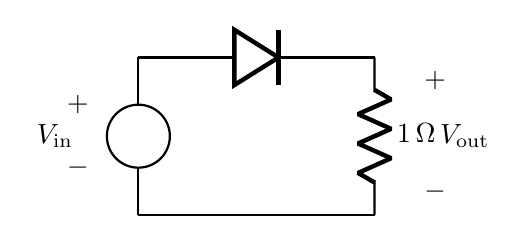
\begin{tikzpicture}[thick,scale=1.0]
            % Input Voltage Source
            \draw (0,1) circle (0.4);
            \node[left] at (-0.5, 1.4) {$+$};
            \node[left] at (-0.5, 0.6) {$-$};
            \node[left] at (-0.7, 1) {$V_{\text{in}}$};
            \draw (0,0) -- (0,0.6);
            \draw (0,1.4) -- (0,2);
            
            % Diode Connection
            \draw (0,2) -- (0.5,2);
            \draw (0.5, 2) to[D] (2.5, 2);
            \draw (2.5,2) -- (3,2);
            
            % Output Resistor (1 Ohm)
            \draw (3,2) to[R, l=$1\,\Omega$] (3,0);
            
            % Output Voltage Labels
            \node[right] at (3.5, 1.7) {$+$};
            \node[right] at (3.5, 0.3) {$-$};
            \node[right] at (3.7, 1) {$V_{\text{out}}$};
            
            % Bottom Wire Connection
            \draw (3,0) -- (0,0);
        \end{tikzpicture}

    % ===================================================
    % Figure 2: V-I Characteristic Graph

        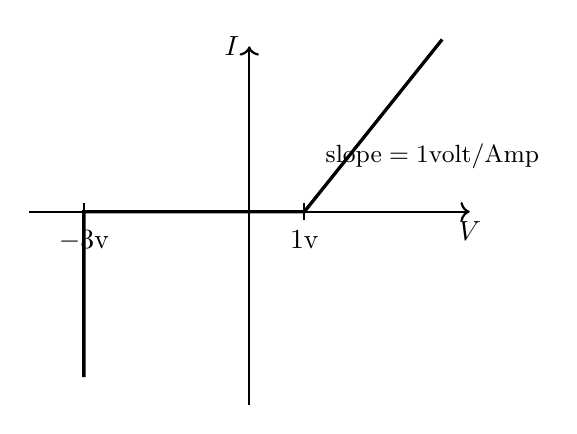
\begin{tikzpicture}[thick,scale=0.7]
            % Axes
            \draw[->] (-4, 0) -- (4, 0) node[below] {$V$};
            \draw[->] (0, -3.5) -- (0, 3) node[left] {$I$};

            % Curve
            \draw[very thick] (-3, -3) -- (-3, 0) -- (1, 0) -- (3.5, 3.125);

            % Labels and Ticks
            \draw (-3, 0.15) -- (-3, -0.15) node[below] {$-3\text{v}$};
            \draw (1, 0.15) -- (1, -0.15) node[below] {$1\text{v}$};
            \node[right] at (1.2, 1.0) {\small $\text{slope} = 1\text{volt/Amp}$};
        \end{tikzpicture}

    % ===================================================
    % Figure 3: Staircase Waveform Graph
    % ===================================================

        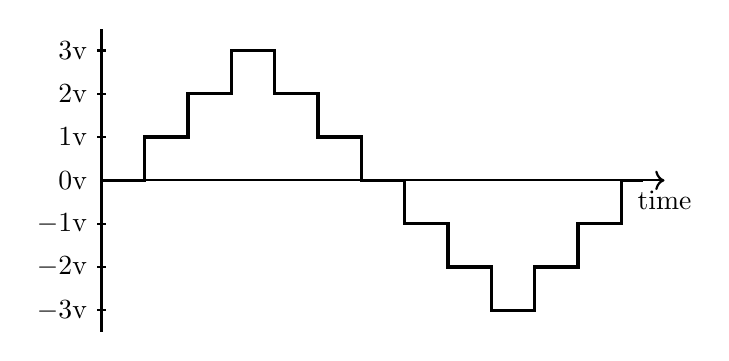
\begin{tikzpicture}[thick,scale=0.55]
            % Axes
            \draw[->] (0, 0) -- (13, 0) node[below] {time};
            \draw (0, -3.5) -- (0, 3.5);

            % Y-axis labels
            \foreach \y in {-3,-2,-1, 1,2,3} {
                \draw (-0.1, \y) -- (0.1, \y);
                \node[left] at (-0.1, \y) {$\y\text{v}$};
            }
            \node[left] at (-0.1, 0) {$0\text{v}$};

            % Staircase Curve
            \draw[very thick] (0,0) 
                -- (1,0) -- (1,1)
                -- (2,1) -- (2,2)
                -- (3,2) -- (3,3)
                -- (4,3) -- (4,2)
                -- (5,2) -- (5,1)
                -- (6,1) -- (6,0)
                -- (7,0) -- (7,-1)
                -- (8,-1) -- (8,-2)
                -- (9,-2) -- (9,-3)
                -- (10,-3) -- (10,-2)
                -- (11,-2) -- (11,-1)
                -- (12,-1) -- (12,0) -- (12.5,0);
        \end{tikzpicture}
\end{center}

\item The I-V characteristics of a diode and a sinusoidal input voltage signal $V_{in}$ are given in the figure. Draw the output voltage $V_{out}$ across the resistor.
\mk{16} 
\item What would be the output voltage $V_{out}$ across the resistor if the diode had a constant 0.7\,V voltage drop?
\mk{10} 

\end{enumerate}

\begin{tcolorbox}[enhanced,breakable,ansbox,colback=cA!4,colframe=cA,boxrule=0.8pt,arc=5pt,title={\textbf{Answer}},fonttitle=\bfseries\color{white},colbacktitle=cA]

\textbf{Preliminary Note on the Input Signal:} 
Although the problem text mentions a ``sinusoidal input voltage signal'', the provided figure explicitly illustrates a staircase waveform. In engineering analysis, when there is a discrepancy between a descriptive text and a provided graphical signal, the explicit graphical waveform is used. The solution below is derived using the staircase waveform.

\subsubsection*{Reference Circuit Diagram}
\begin{center}
\begin{circuitikz}[american, thick, scale=1.0]
    % Input Voltage Source
    \draw (0,1) circle (0.4);
    \node[left] at (-0.5, 1.4) {$+$};
    \node[left] at (-0.5, 0.6) {$-$};
    \node[left] at (-0.7, 1) {$V_{\text{in}}$};
    \draw (0,0) -- (0,0.6);
    \draw (0,1.4) -- (0,2);
    
    % Diode Connection
    \draw (0,2) -- (0.5,2);
    \draw (0.5, 2) to[D] (2.5, 2);
    \draw (2.5,2) -- (3,2);
    
    % Output Resistor (1 Ohm)
    \draw (3,2) to[R, l=$1\,\Omega$] (3,0);
    
    % Output Voltage Labels
    \node[right] at (3.5, 1.7) {$+$};
    \node[right] at (3.5, 0.3) {$-$};
    \node[right] at (3.7, 1) {$V_{\text{out}}$};
    
    % Bottom Wire Connection
    \draw (3,0) -- (0,0);
\end{circuitikz}
\end{center}

\vspace{0.5em}
 
\vspace{0.5em}

\subsubsection*{Part (a): Diode and Resistor in Parallel}

If the diode and the $1\,\Omega$ resistor are connected in parallel, and this combination is directly fed by the input voltage source $V_{in}$ (assuming an ideal voltage source with zero internal resistance), the output voltage $V_{out}$ across the parallel combination is completely dictated by the source. 

By the definition of parallel components connected to an ideal voltage source:
\begin{equation*}
    \mathbf{V_{out} = V_{in}}
\end{equation*}
The waveform for $V_{out}$ will be exactly identical to the input staircase waveform. (Note: The diode would draw current according to its I-V characteristics, but it would not alter the node voltage unless a series source resistance is present, which is not shown).

\vspace{0.5em}
 
\vspace{0.5em}

\subsubsection*{Part (b): $V_{out}$ using the given I-V Characteristics}

\textbf{1. Device Modeling from I-V Curve:}\\
Based on the provided $V-I$ graph, we can extract the piecewise linear model of the diode:
\begin{itemize}
    \item \textbf{Forward Conduction Region:} For $V_D \ge 1\,\text{V}$, the curve has a slope of $1\,\text{A/V}$. Thus, the dynamic forward resistance is $r_d = \frac{1}{\text{slope}} = 1\,\Omega$. The diode behaves as a $1\,\text{V}$ DC source in series with a $1\,\Omega$ resistor.
    \item \textbf{Cutoff Region:} For $-3\,\text{V} < V_D < 1\,\text{V}$, the current is $I_D = 0\,\text{A}$.
    \item \textbf{Breakdown Region:} The diode drops vertically at $V_D = -3\,\text{V}$, indicating a Zener breakdown voltage of $3\,\text{V}$.
\end{itemize}

\textbf{2. Circuit Analysis:}\\
Applying Kirchhoff's Voltage Law (KVL) to the series circuit:
\begin{equation*}
    V_{in} = V_D + V_{out} \quad \text{where} \quad V_{out} = I_D \cdot R = I_D (1\,\Omega)
\end{equation*}

\textit{Case 1: Diode is ON ($V_{in} > 1\,\text{V}$)}\\
Substituting the forward region model $V_D = 1 + I_D(1)$:
\begin{align*}
    V_{in} &= (1 + I_D \cdot 1) + I_D \cdot 1 \\
    V_{in} &= 1 + 2 I_D \\
    I_D &= \frac{V_{in} - 1}{2}
\end{align*}
Since $V_{out} = I_D \cdot 1\,\Omega$, we get:
\begin{equation*}
    V_{out} = \frac{V_{in} - 1}{2} \quad \text{(for } V_{in} > 1\,\text{V})
\end{equation*}

\textit{Case 2: Diode is OFF ($-3\,\text{V} \le V_{in} \le 1\,\text{V}$)}\\
$I_D = 0\,\text{A}$, therefore $V_{out} = 0\,\text{V}$. (Since $V_{in}$ minimum is $-3\,\text{V}$, it never strictly exceeds the breakdown threshold to cause reverse current).

\textbf{3. Waveform Calculation:}\\
Mapping the discrete levels of the input staircase:
\begin{itemize}
    \item $V_{in} = 0\,\text{V}$ to $1\,\text{V} \implies V_{out} = 0\,\text{V}$
    \item $V_{in} = 2\,\text{V} \implies V_{out} = \frac{2 - 1}{2} = 0.5\,\text{V}$
    \item $V_{in} = 3\,\text{V} \implies V_{out} = \frac{3 - 1}{2} = 1.0\,\text{V}$
    \item $V_{in} \le 0\,\text{V} \implies V_{out} = 0\,\text{V}$
\end{itemize}

\textbf{Output Waveform for Part (b):}
\begin{center}
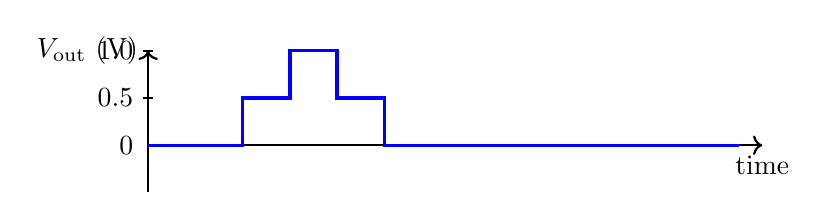
\begin{tikzpicture}[thick,scale=0.6]
    % Axes
    \draw[->] (0, 0) -- (13, 0) node[below] {time};
    \draw[->] (0, -1) -- (0, 2) node[left] {$V_{\text{out}}$ (V)};

    % Y-axis labels
    \foreach \y in {0.5, 1.0} {
        \draw (-0.1, \y*2) -- (0.1, \y*2); % Scale Y by 2 for visibility
        \node[left] at (-0.1, \y*2) {$\y$};
    }
    \node[left] at (-0.1, 0) {$0$};

    % Staircase Curve
    \draw[very thick, blue] (0,0) 
        -- (2,0) -- (2,1)     % Vin goes to 2V at t=2 -> Vout = 0.5V (scaled to 1)
        -- (3,1) -- (3,2)     % Vin goes to 3V at t=3 -> Vout = 1.0V (scaled to 2)
        -- (4,2) -- (4,1)     % Vin goes to 2V at t=4 -> Vout = 0.5V
        -- (5,1) -- (5,0)     % Vin goes to 1V at t=5 -> Vout = 0V
        -- (12.5,0);          % Vin goes negative, Vout stays 0V
\end{tikzpicture}
\end{center}

\vspace{0.5em}
 
\vspace{0.5em}

\subsubsection*{Part (c): $V_{out}$ with Constant Voltage Drop (CVD) Model}

\textbf{1. Device Modeling:}\\
Assume the diode has a Constant Voltage Drop (CVD) of $0.7\,\text{V}$ when forward biased ($r_d = 0\,\Omega$). 
\begin{itemize}
    \item When ON ($V_{in} > 0.7\,\text{V}$): $V_D = 0.7\,\text{V}$.
    \item When OFF ($V_{in} < 0.7\,\text{V}$): $I_D = 0\,\text{A}$.
\end{itemize}

\textbf{2. Circuit Analysis:}\\
Applying KVL:
\begin{equation*}
    V_{out} = \begin{cases} 
      V_{in} - 0.7\,\text{V}, & V_{in} > 0.7\,\text{V} \\
      0\,\text{V}, & V_{in} \le 0.7\,\text{V}
   \end{cases}
\end{equation*}

\textbf{3. Waveform Calculation:}\\
Mapping the discrete levels of the input staircase:
\begin{itemize}
    \item $V_{in} = 0\,\text{V} \implies V_{out} = 0\,\text{V}$
    \item $V_{in} = 1\,\text{V} \implies V_{out} = 1 - 0.7 = 0.3\,\text{V}$
    \item $V_{in} = 2\,\text{V} \implies V_{out} = 2 - 0.7 = 1.3\,\text{V}$
    \item $V_{in} = 3\,\text{V} \implies V_{out} = 3 - 0.7 = 2.3\,\text{V}$
    \item $V_{in} \le 0\,\text{V} \implies V_{out} = 0\,\text{V}$
\end{itemize}

\textbf{Output Waveform for Part (c):}
\begin{center}
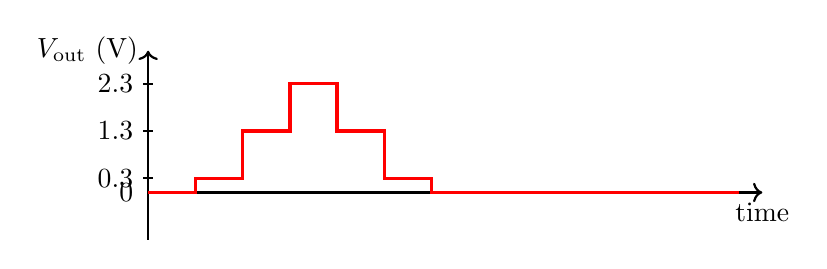
\begin{tikzpicture}[thick,scale=0.6]
    % Axes
    \draw[->] (0, 0) -- (13, 0) node[below] {time};
    \draw[->] (0, -1) -- (0, 3) node[left] {$V_{\text{out}}$ (V)};

    % Y-axis labels
    \foreach \y in {0.3, 1.3, 2.3} {
        \draw (-0.1, \y) -- (0.1, \y);
        \node[left] at (-0.1, \y) {$\y$};
    }
    \node[left] at (-0.1, 0) {$0$};

    % Staircase Curve
    \draw[very thick, red] (0,0) 
        -- (1,0) -- (1,0.3)   % Vin goes to 1V -> Vout = 0.3V
        -- (2,0.3) -- (2,1.3) % Vin goes to 2V -> Vout = 1.3V
        -- (3,1.3) -- (3,2.3) % Vin goes to 3V -> Vout = 2.3V
        -- (4,2.3) -- (4,1.3) % Vin goes to 2V -> Vout = 1.3V
        -- (5,1.3) -- (5,0.3) % Vin goes to 1V -> Vout = 0.3V
        -- (6,0.3) -- (6,0)   % Vin goes to 0V -> Vout = 0V
        -- (12.5,0);          % Vin stays negative, Vout stays 0V
\end{tikzpicture}
\end{center}

\end{tcolorbox}

\item
\begin{enumerate}
\item An AC voltage source is applied to a series combination of a diode and a resistance. The dotted line in the figure is the input voltage waveform ($V_{ac}$) and the solid line is the output voltage waveform ($V_R$) across the resistance. Copy $V_R$ from the figure to your answer script exactly to scale and draw the voltage waveform across the diode over the same graph. Given that $\frac{dV_{ac}}{dt}=1\,\text{V/sec}$ when $V_{ac}$ is rising and $\frac{dV_{ac}}{dt}=-1\,\text{V/sec}$ when $V_{ac}$ is falling.

\begin{center}
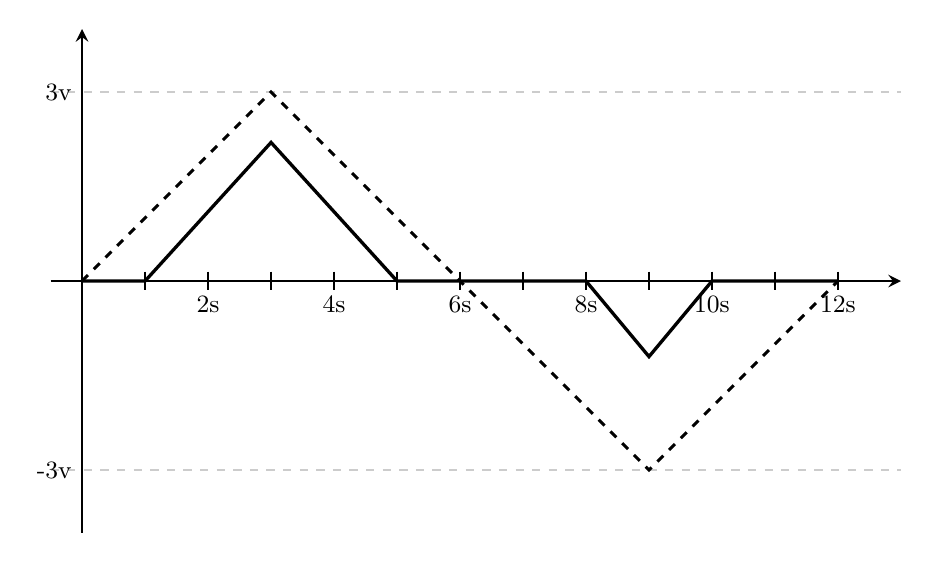
\begin{tikzpicture}[thick,scale=0.8]
    % ৩ভোল্ট এবং -৩ভোল্ট এর অনুভূমিক ডটেড গাইডলাইন
    \draw[gray!40, dashed] (-0.5, 3) -- (13, 3);
    \draw[gray!40, dashed] (-0.5, -3) -- (13, -3);
    
    % Y-axis এর লেবেল (3v এবং -3v)
    \node[left, font=\small] at (0, 3) {3v};
    \node[left, font=\small] at (0, -3) {-3v};

    % অক্ষরেখা (Axes) অংকন
    \draw[->, >=stealth, line width=1pt] (-0.5, 0) -- (13, 0); % X-axis
    \draw[->, >=stealth, line width=1pt] (0, -4) -- (0, 4);   % Y-axis

    % X-axis এর প্রতিটি ১ সেকেন্ড পর পর টিক মার্ক (Ticks)
    \foreach \x in {1,2,...,12} {
        \draw (\x, 0.15) -- (\x, -0.15);
    }
    
    % ছবিতে থাকা নির্দিষ্ট টাইম লেবেলগুলো (2s, 4s, 6s, 8s, 10s, 12s)
    \node[below, font=\small, yshift=-2pt] at (2, 0) {2s};
    \node[below, font=\small, yshift=-2pt] at (4, 0) {4s};
    \node[below, font=\small, yshift=-2pt] at (6, 0) {6s};
    \node[below, font=\small, yshift=-2pt] at (8, 0) {8s};
    \node[below, font=\small, yshift=-2pt] at (10, 0) {10s};
    \node[below, font=\small, yshift=-2pt] at (12, 0) {12s};

    % ১. ড্যাশড ওয়েভফর্ম (Dashed Triangle Wave)
    % (0,0) থেকে শুরু হয়ে 3s এ পিক (3v), 6s এ শূন্য, 9s এ নেগেটিভ পিক (-3v), 12s এ শেষ।
    \draw[dashed, line width=1.1pt] (0,0) -- (3,3) -- (6,0) -- (9,-3) -- (12,0);

    % ২. সলিড ওয়েভফর্ম (Solid Output Waveform)
    % ছবি অনুযায়ী: 1s পর্যন্ত 0, তারপর 3s এ পজিটিভ পিক, 5s এ আবার 0। 
    % এরপর 8s পর্যন্ত 0, 9s এ ছোট নেগেটিভ পিক, এবং 10s থেকে 12s পর্যন্ত আবার 0।
    \draw[very thick, black] (0,0) -- (1,0) -- (3,2.2) -- (5,0) -- (8,0) -- (9,-1.2) -- (10,0) -- (12,0);

\end{tikzpicture}
\end{center}

\mk{20} \yr{EEE 263 | L-2/T-1 | 2012--13}




\item Draw the I-V characteristics curve of the above diode exactly to scale (mention the voltage(s) at which the diode begins conduction).
\mk{16} \yr{EEE 263 | L-2/T-1 | 2012--13}

\item Draw the voltage waveform across the diode if it had been connected in parallel to the resistance.
\mk{10} \yr{EEE 263 | L-2/T-1 | 2012--13}

\end{enumerate}

\begin{tcolorbox}[enhanced,breakable,ansbox,colback=cA!4,colframe=cA,boxrule=0.8pt,arc=5pt,title={\textbf{Answer}},fonttitle=\bfseries\color{white},colbacktitle=cA]

\subsubsection*{Part (a): Graphical Derivation and Diode Voltage Waveform ($V_D$)}

By Kirchhoff's Voltage Law (KVL) applied to the series circuit loop:
\begin{equation*}
    V_{ac}(t) = V_D(t) + V_R(t) \implies \mathbf{V_D(t) = V_{ac}(t) - V_R(t)}
\end{equation*}

The diode voltage at any instant is found by subtracting the coordinates of the resistor voltage ($V_R$) from the input AC voltage ($V_{ac}$). Computing the key boundary transitions:
\begin{itemize}
    \item \textbf{From $0\,\text{s}$ to $1\,\text{s}$:} $V_{ac}$ rises from $0\,\text{V}$ to $1\,\text{V}$ while $V_R = 0\,\text{V} \implies V_D = V_{ac}$. At $t = 1\,\text{s}$, $V_D = 1\,\text{V}$.
    \item \textbf{At $t = 3\,\text{s}$ (Positive Peak):} $V_{ac} = 3\,\text{V}$, $V_R = 2.2\,\text{V} \implies V_D = 3 - 2.2 = 0.8\,\text{V}$.
    \item \textbf{At $t = 5\,\text{s}$:} $V_{ac} = 1\,\text{V}$, $V_R = 0\,\text{V} \implies V_D = 1\,\text{V}$.
    \item \textbf{At $t = 6\,\text{s}$:} $V_{ac} = 0\,\text{V}$, $V_R = 0\,\text{V} \implies V_D = 0\,\text{V}$.
    \item \textbf{At $t = 8\,\text{s}$:} $V_{ac} = -2\,\text{V}$, $V_R = 0\,\text{V} \implies V_D = -2\,\text{V}$.
    \item \textbf{At $t = 9\,\text{s}$ (Negative Peak):} $V_{ac} = -3\,\text{V}$, $V_R = -1.2\,\text{V} \implies V_D = -3 - (-1.2) = -1.8\,\text{V}$.
    \item \textbf{At $t = 10\,\text{s}$:} $V_{ac} = -2\,\text{V}$, $V_R = 0\,\text{V} \implies V_D = -2\,\text{V}$.
    \item \textbf{At $t = 12\,\text{s}$:} $V_{ac} = 0\,\text{V}$, $V_R = 0\,\text{V} \implies V_D = 0\,\text{V}$.
\end{itemize}

Below is the complete waveform graph containing $V_{ac}$ (dashed gray), $V_R$ (solid black), and the derived $V_D$ (\textbf{solid blue line}):

\begin{center}
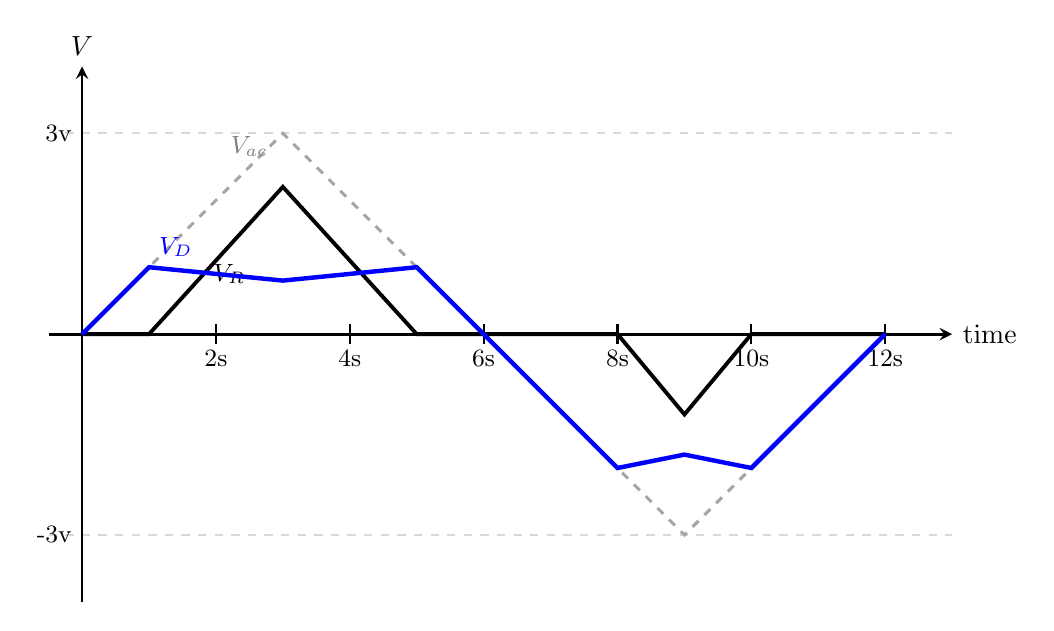
\begin{tikzpicture}[thick,scale=0.85]
    % Guidelines
    \draw[gray!30, dashed] (-0.5, 3) -- (13, 3);
    \draw[gray!30, dashed] (-0.5, -3) -- (13, -3);
    
    % Labels
    \node[left, font=\small] at (0, 3) {3v};
    \node[left, font=\small] at (0, -3) {-3v};

    % Axes
    \draw[->, >=stealth, line width=1pt] (-0.5, 0) -- (13, 0) node[right] {time}; 
    \draw[->, >=stealth, line width=1pt] (0, -4) -- (0, 4) node[above] {$V$};   

    % Ticks
    \foreach \x in {2,4,6,8,10,12} {
        \draw (\x, 0.15) -- (\x, -0.15);
        \node[below, font=\small, yshift=-2pt] at (\x, 0) {\x s};
    }

    % Input Waveform (Vac) - Dashed Gray
    \draw[dashed, line width=1.1pt, gray!70] (0,0) -- (3,3) -- (6,0) -- (9,-3) -- (12,0);
    \node[gray, font=\small, above] at (2.5, 2.5) {$V_{ac}$};

    % Resistor Output Waveform (VR) - Solid Black
    \draw[line width=1.4pt, black] (0,0) -- (1,0) -- (3,2.2) -- (5,0) -- (8,0) -- (9,-1.2) -- (10,0) -- (12,0);
    \node[black, font=\small, below] at (2.2, 1.2) {$V_R$};

    % Diode Waveform (VD) - Solid Blue
    \draw[line width=1.6pt, blue] (0,0) -- (1,1) -- (3,0.8) -- (5,1) -- (6,0) -- (8,-2) -- (9,-1.8) -- (10,-2) -- (12,0);
    \node[blue, font=\small, above] at (1.4, 1.0) {$V_D$};
\end{tikzpicture}
\end{center}

\vspace{0.5em}
 
\vspace{0.5em}

\subsubsection*{Part (b): I-V Characteristics Curve of the Diode}

By tracking the relationship between the diode voltage $V_D$ and the loop current $I = \frac{V_R}{R}$, we deduce the behavioral model of this unique device:
\begin{enumerate}
    \item \textbf{Forward Conduction Threshold:} Forward conduction begins precisely at $\mathbf{V_D = 1\,\text{V}}$ (corresponding to $t=1\,\text{s}$ where $V_R$ begins rising from $0\,\text{V}$). As current increases up to a peak value of $I_{max} = \frac{2.2}{R}$, the voltage across the diode drops slightly down to $0.8\,\text{V}$, revealing a negative dynamic differential resistance ($r_d < 0$).
    \item \textbf{Reverse Conduction (Breakdown) Threshold:} Reverse conduction begins at $\mathbf{V_D = -2\,\text{V}}$ (corresponding to $t=8\,\text{s}$). As reverse current increases in magnitude to a peak value of $I = -\frac{1.2}{R}$, the voltage shifts to $-1.8\,\text{V}$.
    \item \textbf{Non-Conducting (Off) State:} For $-2\,\text{V} \le V_D \le 1\,\text{V}$, the current through the device is $I = 0\,\text{A}$.
\end{enumerate}

\begin{center}
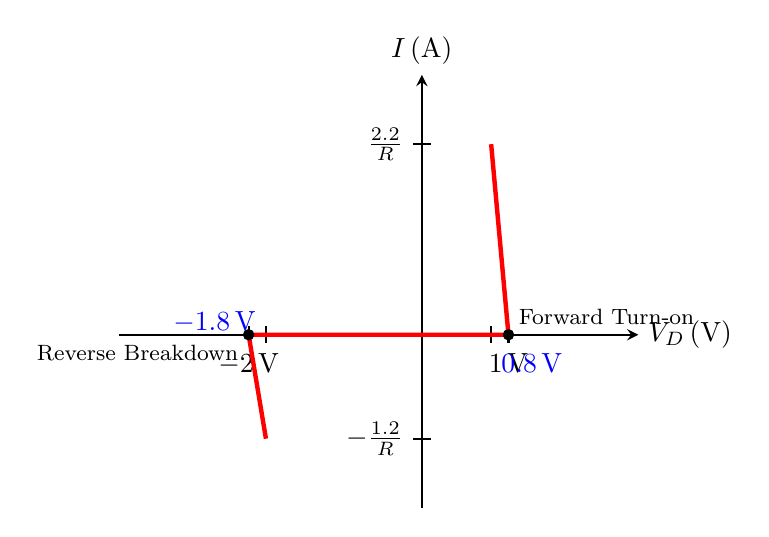
\begin{tikzpicture}[thick,scale=1.1]
    % Axes
    \draw[->, >=stealth] (-3.5, 0) -- (2.5, 0) node[right] {$V_D\,\text{(V)}$};
    \draw[->, >=stealth] (0, -2) -- (0, 3) node[above] {$I\,\text{(A)}$};
    
    % Axis tick indicators
    \draw (-2, 0.1) -- (-2, -0.1) node[below] {$-2\,\text{V}$};
    \draw (-1.8, 0.1) -- (-1.8, -0.1) node[above left, blue] {$-1.8\,\text{V}$};
    \draw (1, 0.1) -- (1, -0.1) node[below] {$1\,\text{V}$};
    \draw (0.8, 0.1) -- (0.8, -0.1) node[below right, blue] {$0.8\,\text{V}$};
    
    \draw (0.1, 2.2) -- (-0.1, 2.2) node[left] {$\frac{2.2}{R}$};
    \draw (0.1, -1.2) -- (-0.1, -1.2) node[left] {$-\frac{1.2}{R}$};
    
    % I-V Plot
    \draw[ultra thick, red] (-1.8, -1.2) -- (-2, 0) -- (1, 0) -- (0.8, 2.2);
    
    % Highlighting Turn-on points
    \filldraw[black] (1,0) circle (1.5pt) node[above right, font=\footnotesize] {Forward Turn-on};
    \filldraw[black] (-2,0) circle (1.5pt) node[below left, font=\footnotesize] {Reverse Breakdown};
\end{tikzpicture}
\end{center}

\vspace{0.5em}
 
\vspace{0.5em}

\subsubsection*{Part (c): Diode Connected in Parallel with the Resistance}

When the diode is connected in parallel with the resistance across an ideal independent AC voltage source, the voltage at the output nodes is entirely governed by the source itself. 

By the fundamental definition of parallel connections across an ideal source:
\begin{equation*}
    V_D(t) = V_R(t) = V_{ac}(t)
\end{equation*}

Consequently, the diode does not split the source voltage with another series element. The voltage waveform across it will perfectly duplicate the input triangular waveform $V_{ac}$:

\begin{center}
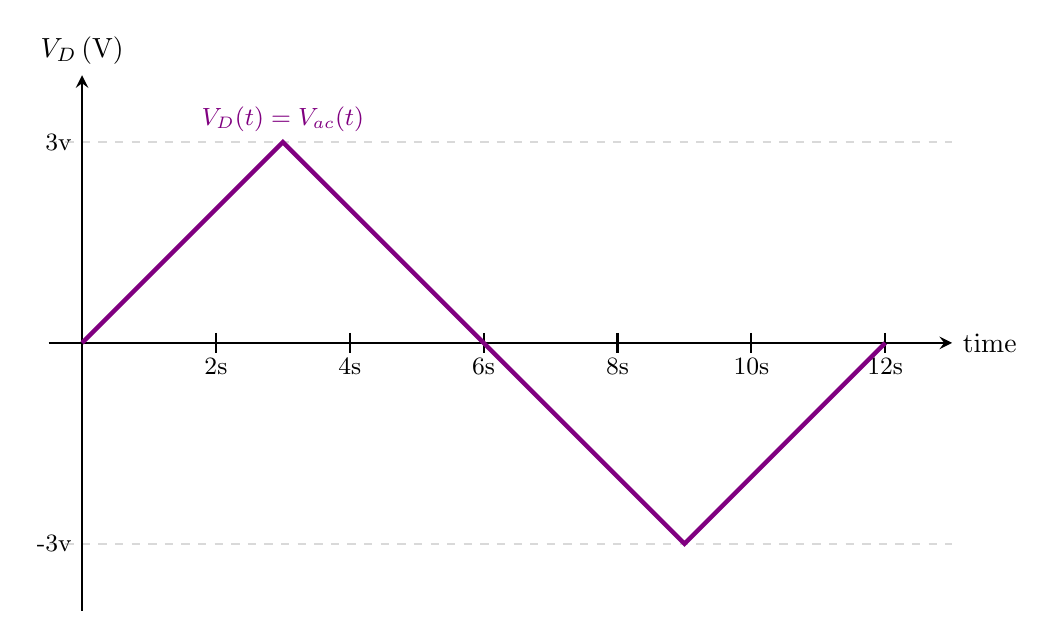
\begin{tikzpicture}[thick,scale=0.85]
    % Guidelines
    \draw[gray!30, dashed] (-0.5, 3) -- (13, 3);
    \draw[gray!30, dashed] (-0.5, -3) -- (13, -3);
    \node[left, font=\small] at (0, 3) {3v};
    \node[left, font=\small] at (0, -3) {-3v};

    % Axes
    \draw[->, >=stealth, line width=1pt] (-0.5, 0) -- (13, 0) node[right] {time};
    \draw[->, >=stealth, line width=1pt] (0, -4) -- (0, 4) node[above] {$V_D\,\text{(V)}$};

    % Ticks
    \foreach \x in {2,4,6,8,10,12} {
        \draw (\x, 0.15) -- (\x, -0.15);
        \node[below, font=\small, yshift=-2pt] at (\x, 0) {\x s};
    }

    % Parallel Diode Waveform (Matches Vac exactly)
    \draw[ultra thick, violet] (0,0) -- (3,3) -- (6,0) -- (9,-3) -- (12,0);
    \node[violet, font=\small, above] at (3, 3) {$V_D(t) = V_{ac}(t)$};
\end{tikzpicture}
\end{center}

\end{tcolorbox}

\end{enumerate}

%%──────────────────────────────────────────────────────────────────────
\subtopic{cA}{Diode Thermal Characteristics}
\label{sub:s1-thermal}

\begin{enumerate}
    
\item When a 15\,A current is applied to a particular diode, the junction voltage immediately becomes 0.7\,V. As power dissipation raises its temperature, the voltage eventually reaches 0.6\,V. (i) What is the apparent rise in junction temperature? (ii) What is the temperature rise per watt of power dissipation? (iii) What is the power dissipated in the diode in its final state?
\mk{15} \yr{EEE 263 | L-2/T-1 | 2024--25}

\begin{tcolorbox}[enhanced,breakable,ansbox,colback=cA!4,colframe=cA,boxrule=0.8pt,arc=5pt,title={\textbf{Answer}},fonttitle=\bfseries\color{white},colbacktitle=cA]

\textbf{Theory and Assumptions}

For a standard silicon pn-junction diode, the forward voltage drop $V_D$ exhibits a negative temperature coefficient when operated at a constant forward current. As the temperature of the junction increases, the forward voltage required to maintain the same current decreases linearly. 

A widely accepted standard approximation in analog circuit design for the temperature coefficient of a silicon diode is:
\begin{equation}
    k = \frac{\Delta V_D}{\Delta T} \approx -2.0 \, \text{mV}/^\circ\text{C}
\end{equation}
This means that for every $1^\circ\text{C}$ rise in junction temperature, the diode voltage drops by approximately $2 \, \text{mV}$. We will use this standard assumption to determine the temperature rise.

\vspace{0.5cm}

\textbf{Test Circuit Equivalent Diagram}

The following schematic models the testing condition described in the problem, where an ideal constant current source drives the diode, and the resulting voltage is measured.

\begin{center}
\begin{circuitikz}[american, thick]
    % Draw the circuit
    \draw (0,0) to[I, l=$I_D$, a=15\,\text{A}, color=blue] (0,3)
          -- (3,3)
          to[full diode, v=$V_D$, name=D1] (3,0)
          -- (0,0);
    
    % Add ground
    \node[ground] at (1.5,0) {};
    
    % Add node labels and voltage polarity indication
    \node[anchor=south] at (0,3) {\textbf{A}};
    \node[anchor=south] at (3,3) {\textbf{B}};
    \draw[color=red, ->, >=stealth] (3.8, 2.5) -- (3.8, 0.5) node[midway, right] {$I_D$};
\end{circuitikz}
\end{center}

\vspace{0.5cm}

\textbf{Given Data}
\begin{itemize}
    \item Constant forward current, $I_D = 15 \, \text{A}$
    \item Initial junction voltage, $V_{D1} = 0.7 \, \text{V}$
    \item Final steady-state junction voltage, $V_{D2} = 0.6 \, \text{V}$
\end{itemize}

\vspace{0.5cm}

\textbf{Step-by-Step Solution}

\textbf{(i) Apparent Rise in Junction Temperature}

First, we determine the total change in the junction voltage:
\begin{align*}
    \Delta V_D &= V_{D2} - V_{D1} \\
    &= 0.6 \, \text{V} - 0.7 \, \text{V} \\
    &= -0.1 \, \text{V} \\
    &= -100 \, \text{mV}
\end{align*}

Using the standard temperature coefficient $k = -2.0 \, \text{mV}/^\circ\text{C}$, the apparent rise in junction temperature ($\Delta T$) can be calculated as:
\begin{align*}
    \Delta T &= \frac{\Delta V_D}{k} \nonumber \\
    &= \frac{-100 \, \text{mV}}{-2.0 \, \text{mV}/^\circ\text{C}} \nonumber \\
    &= 50^\circ\text{C}
\end{align*}
The junction temperature of the diode rises by $50^\circ\text{C}$ relative to the ambient or initial state.

\vspace{0.5cm}

\textbf{(iii) Power Dissipated in the Diode in its Final State}

\textit{Note: We compute the final power first, as it represents the steady-state condition necessary to evaluate the thermal resistance required in part (ii).}

The power dissipated by the diode at any given moment is the product of the forward voltage and the constant forward current. In the final state (thermal equilibrium), the voltage has settled at $V_{D2} = 0.6 \, \text{V}$.
\begin{align*}
    P_{\text{final}} &= V_{D2} \times I_D \nonumber \\
    &= 0.6 \, \text{V} \times 15 \, \text{A} \nonumber \\
    &= 9.0 \, \text{W}
\end{align*}

\vspace{0.5cm}

\textbf{(ii) Temperature Rise per Watt of Power Dissipation}

The temperature rise per watt of power dissipation characterizes the thermal resistance ($\theta_{JA}$ or thermal resistance from junction to ambient) of the diode assembly. Since the diode temperature reaches a stable plateau, the relevant power causing this steady-state temperature rise is the final power dissipation ($P_{\text{final}}$).

\begin{align*}
    \theta &= \frac{\Delta T}{P_{\text{final}}} \nonumber \\
    &= \frac{50^\circ\text{C}}{9.0 \, \text{W}} \nonumber \\
    &\approx 5.556^\circ\text{C/W}
\end{align*}

\vspace{0.5cm}

\begin{center}
\renewcommand{\arraystretch}{1.5}
\begin{tabular}{|>{\bfseries}l|c|}
\hline
\rowcolor{cA!20} \multicolumn{2}{|c|}{\textbf{Final Answers Summary}} \\
\hline
(i) Apparent Rise in Junction Temperature ($\Delta T$) & $50^\circ\text{C}$ \\
\hline
(ii) Temperature Rise per Watt ($\theta$) & $5.56^\circ\text{C/W}$ \\
\hline
(iii) Final Steady-State Power Dissipation ($P_{\text{final}}$) & $9.0 \, \text{W}$ \\
\hline
\end{tabular}
\end{center}

\end{tcolorbox}

\item When a 15\,A current is applied to a particular diode, the junction voltage immediately becomes 0.7\,V. As power dissipation raises its temperature, the voltage eventually reaches 0.58\,V.\\
 (i) What is the apparent rise in junction temperature? \\
 (ii) What is the temperature rise per watt of power dissipation? \\
 (iii) What is the power dissipated in the diode in its final state?\\
\mk{10} \yr{EEE 263 | L-2/T-1 | 2023--24}

\begin{tcolorbox}[enhanced,breakable,ansbox,colback=cA!4,colframe=cA,boxrule=0.8pt,arc=5pt,title={\textbf{Answer}},fonttitle=\bfseries\color{white},colbacktitle=cA]

\textbf{Theory and Assumptions}

For standard silicon pn-junction diodes, the forward voltage drop $V_D$ decreases linearly as the junction temperature increases, provided the forward current remains constant. 

A standard textbook approximation for the temperature coefficient of a silicon diode's forward voltage is:
\begin{equation}
    k = \frac{\Delta V_D}{\Delta T} \approx -2.0 \, \text{mV}/^\circ\text{C}
\end{equation}
This indicates that the junction voltage decreases by approximately $2 \, \text{mV}$ for every $1^\circ\text{C}$ rise in the diode's junction temperature.

\vspace{0.5cm}

\textbf{Test Circuit Equivalent Diagram}

The circuit diagram below models the test condition. An ideal constant current source drives the diode, and the resulting voltage is measured across its terminals.

\begin{center}
\begin{circuitikz}[american, thick]
    % Draw the circuit
    \draw (0,0) to[I, l=$I_D$, a=15\,\text{A}, color=blue] (0,3)
          -- (3,3)
          to[full diode, v=$V_D$,name=D1] (3,0)
          -- (0,0);
    
    % Add ground
    \node[ground] at (1.5,0) {};
    
    % Add node labels and voltage polarity indication
    \node[anchor=south] at (0,3) {\textbf{A}};
    \node[anchor=south] at (3,3) {\textbf{B}};
    \draw[color=red, ->, >=stealth] (3.8, 2.5) -- (3.8, 0.5) node[midway, right] {$I_D$};
\end{circuitikz}
\end{center}

\vspace{0.5cm}

\textbf{Given Data}
\begin{itemize}
    \item Constant forward current, $I_D = 15 \, \text{A}$
    \item Initial junction voltage, $V_{D1} = 0.7 \, \text{V}$
    \item Final steady-state junction voltage, $V_{D2} = 0.58 \, \text{V}$
\end{itemize}

\vspace{0.5cm}

\textbf{Step-by-Step Solution}

\textbf{(i) Apparent Rise in Junction Temperature}

First, we calculate the total change in the diode's forward voltage:
\begin{align*}
    \Delta V_D &= V_{D2} - V_{D1} \\
    &= 0.58 \, \text{V} - 0.70 \, \text{V} \\
    &= -0.12 \, \text{V} \\
    &= -120 \, \text{mV}
\end{align*}

Using the standard temperature coefficient $k = -2.0 \, \text{mV}/^\circ\text{C}$, the apparent rise in junction temperature ($\Delta T$) is:
\begin{align*}
    \Delta T &= \frac{\Delta V_D}{k} \nonumber \\
    &= \frac{-120 \, \text{mV}}{-2.0 \, \text{mV}/^\circ\text{C}} \nonumber \\
    &= 60^\circ\text{C}
\end{align*}
The junction temperature of the diode rises by $60^\circ\text{C}$ relative to its initial state.

\vspace{0.5cm}

\textbf{(iii) Power Dissipated in the Diode in its Final State}

\textit{Note: Calculating the final power state first provides the steady-state thermal conditions needed to evaluate the thermal resistance required in part (ii).}

The power dissipated by the diode at steady-state is the product of the final forward voltage and the constant forward current.
\begin{align*}
    P_{\text{final}} &= V_{D2} \times I_D \nonumber \\
    &= 0.58 \, \text{V} \times 15 \, \text{A} \nonumber \\
    &= 8.7 \, \text{W}
\end{align*}

\vspace{0.5cm}

\textbf{(ii) Temperature Rise per Watt of Power Dissipation}

The temperature rise per watt of power dissipation represents the effective thermal resistance ($\theta_{JA}$) of the system. Since the diode has reached a stable equilibrium, we use the final steady-state power dissipation ($P_{\text{final}}$).

\begin{align*}
    \theta &= \frac{\Delta T}{P_{\text{final}}} \nonumber \\
    &= \frac{60^\circ\text{C}}{8.7 \, \text{W}} \nonumber \\
    &\approx 6.897^\circ\text{C/W}
\end{align*}

\vspace{0.5cm}

\begin{center}
\renewcommand{\arraystretch}{1.5}
\begin{tabular}{|>{\bfseries}l|c|}
\hline
\rowcolor{cA!20} \multicolumn{2}{|c|}{\textbf{Final Answers Summary}} \\
\hline
(i) Apparent Rise in Junction Temperature ($\Delta T$) & $60^\circ\text{C}$ \\
\hline
(ii) Temperature Rise per Watt ($\theta$) & $6.90^\circ\text{C/W}$ \\
\hline
(iii) Final Steady-State Power Dissipation ($P_{\text{final}}$) & $8.7 \, \text{W}$ \\
\hline
\end{tabular}
\end{center}

\end{tcolorbox}

\end{enumerate}

%%──────────────────────────────────────────────────────────────────────
\subtopic{cA}{Bridge Rectifier}
\label{sub:s1-rectifier}

\begin{enumerate}
    
\item Consider a bridge rectifier circuit with a filter capacitor $C$ placed across the load resistor $R=100\,\Omega$. The transformer secondary delivers a sinusoid of 12\,V (rms) at 60\,Hz. Assume $V_D=0.8\,\text{V}$.\\
 (i) Find the value of $C$ such that the ripple voltage is no larger than 1\,V peak-to-peak. \\
 (ii) What is the DC voltage at the output? \\
 (iii) Find the load current. \\
 (iv) Find the average and peak diode currents. \\
 (v) What is the peak reverse voltage across each diode?\\
\mk{15} \yr{EEE 263 | L-2/T-1 | 2023--24}

\begin{tcolorbox}[enhanced,breakable,ansbox,colback=cA!4,colframe=cA,boxrule=0.8pt,arc=5pt,title={\textbf{Answer}},fonttitle=\bfseries\color{white},colbacktitle=cA]

\textbf{Theory and Circuit Operation}

A bridge rectifier utilizes four diodes arranged in a bridge configuration to convert an alternating current (AC) input into a pulsating direct current (DC) output. By adding a filter capacitor $C$ in parallel with the load resistor $R$, the output voltage is smoothed out into a DC voltage with a small ripple component.

\begin{enumerate}
    \item \textbf{Positive Half-Cycle:} When the secondary voltage is positive, diodes $D_1$ and $D_4$ are forward-biased (ON), while $D_2$ and $D_3$ are reverse-biased (OFF). Current flows from the transformer through $D_1$, through the load network ($R \parallel C$), and returns through $D_4$.
    \item \textbf{Negative Half-Cycle:} When the secondary voltage reverses, diodes $D_2$ and $D_3$ become forward-biased (ON), while $D_1$ and $D_4$ turn OFF. Current flows through $D_2$, through the load network in the same direction as before, and returns through $D_3$.
    \item \textbf{Filter Operation:} The capacitor charges to the peak value of the rectified voltage ($V_p$) during the conduction intervals. When the input voltage falls below the capacitor voltage, the diodes turn off, and the capacitor discharges through the load resistor $R$ with a time constant $\tau = RC$. Because this occurs twice per line cycle, the ripple frequency is $f_r = 2f$.
\end{enumerate}

\vspace{0.3cm}

\textbf{Circuit Schematic}

\begin{center}
\begin{circuitikz}[thick]
    
    % AC Source (Transformer Secondary)
    \draw (0,0) to[sV] (0,-4);
    \node[left, align=center] at (-0.8,-2) {Secondary \\ $12\,\text{V}_{\text{rms}}$ \\ $60\,\text{Hz}$};
    
    % AC Routing to Bridge Rectifier
    % Top AC line to left node of the bridge
    \draw (0,0) -- (1.5,0) -- (1.5,-2) -- (3,-2);
    % Bottom AC line to right node of the bridge (routed completely around)
    \draw (0,-4) -- (1.5,-4) -- (1.5,-6) -- (8,-6) -- (8,-2) -- (7,-2);
    
    % Bridge Rectifier Diodes
    \draw (3,-2) to[D, l=$D_1$] (5,0);
    \draw (7,-2) to[D, l_=$D_2$] (5,0);
    \draw (5,-4) to[D, l=$D_3$] (3,-2);
    \draw (5,-4) to[D, l_=$D_4$] (7,-2);
    
    % Bridge Connection Nodes
    \node[circ] at (3,-2) {};
    \node[circ] at (7,-2) {};
    \node[circ] at (5,0) {};
    \node[circ] at (5,-4) {};
    
    % DC Rails
    \draw (5,0) -- (13,0);
    \draw (5,-4) -- (13,-4);
    
    % Filter Capacitor
    \draw (10,0) to[C, l=$C$, *-*] (10,-4);
    
    % Ground (centered between C and R)
    \draw (11.5,-4) to[short, *-] (11.5,-4.5) node[ground]{};
    
    % Load Resistor
    \draw (13,0) to[R, l={$R=100\,\Omega$}] (13,-4);

\end{circuitikz}

\end{center}

\vspace{0.3cm}

\textbf{Mathematical Derivations}

The peak value of the secondary voltage ($V_{sm}$) is given by:
\begin{equation}
    V_{sm} = V_{s,\text{rms}} \times \sqrt{2}
\end{equation}
Since two diodes conduct simultaneously during each half-cycle in a bridge rectifier, the peak rectified output voltage ($V_p$) across the capacitor is reduced by two diode drops:
\begin{equation}
    V_p = V_{sm} - 2V_D
\end{equation}
For a full-wave rectifier with a heavy filter capacitor ($RC \gg T$), the peak-to-peak ripple voltage ($V_r$) can be approximated using the linear discharge model:
\begin{equation}
    V_r = \frac{V_p}{2fRC} = \frac{I_L}{2fC}
\end{equation}
where $f$ is the input line frequency ($60\,\text{Hz}$).

\vspace{0.5cm}

\textbf{Step-by-Step Solution}

Given Parameters:
\begin{align*}
    V_{s,\text{rms}} &= 12\,\text{V}, \quad f = 60\,\text{Hz}, \quad R = 100\,\Omega, \quad V_D = 0.8\,\text{V}, \quad V_r \le 1\,\text{V}
\end{align*}

First, compute the input peak voltage:
\begin{align*}
    V_{sm} &= 12 \times \sqrt{2} \approx 16.971\,\text{V}
\end{align*}
Next, compute the peak output voltage:
\begin{align*}
    V_p &= 16.971 - 2(0.8) = 15.371\,\text{V}
\end{align*}

\vspace{0.3cm}

\textbf{(i) Find the value of $C$ for $V_r \le 1\,\text{V}$}

Rearranging the ripple voltage formula to solve for $C$:
\begin{align*}
    C &= \frac{V_p}{2fR V_r} \nonumber \\
    &= \frac{15.371}{2 \times 60 \times 100 \times 1} \nonumber \\
    &= \frac{15.371}{12000} \approx 1.2809 \times 10^{-3}\,\text{F} = 1281\,\mu\text{F}
\end{align*}

\vspace{0.3cm}

\textbf{(ii) Determine the DC output voltage}

The average or DC voltage ($V_{DC}$) at the output is the peak value minus half of the peak-to-peak ripple voltage:
\begin{align*}
    V_{DC} &= V_p - \frac{1}{2}V_r \nonumber \\
    &= 15.371 - \frac{1}{2}(1) = 14.871\,\text{V}
\end{align*}

\vspace{0.3cm}

\textbf{(iii) Find the load current}

The average load current ($I_L$) is calculated via Ohm's law using the DC output voltage:
\begin{align*}
    I_L &= \frac{V_{DC}}{R} \nonumber \\
    &= \frac{14.871}{100} = 0.1487\,\text{A} = 148.71\,\text{mA}
\end{align*}

\vspace{0.3cm}

\textbf{(iv) Find the average and peak diode currents}

Using the standard textbook equations for diode currents in full-wave capacitor-filter circuits:
\begin{enumerate}
    \item \textbf{Peak Diode Current ($I_{D,\text{peak}}$):}
    \begin{align*}
        I_{D,\text{peak}} &= I_L \left(1 + 2\pi\sqrt{\frac{V_p}{2V_r}}\right) \nonumber \\
        &= 0.14871 \times \left(1 + 2\pi\sqrt{\frac{15.371}{2 \times 1}}\right) \nonumber \\
        &= 0.14871 \times \left(1 + 2\pi\sqrt{7.6855}\right) \nonumber \\
        &= 0.14871 \times \left(1 + 2\pi \times 2.7723\right) \nonumber \\
        &= 0.14871 \times \left(1 + 17.419\right) = 0.14871 \times 18.419 \approx 2.739\,\text{A}
    \end{align*}
    
    \item \textbf{Average Diode Current ($I_{D,\text{avg}}$):}
    \begin{itemize}
        \item \textit{Over a full cycle:} Each diode conducts for only one half-cycle, sharing the total load current equally over time.
        \begin{align*}
            I_{D,\text{avg}} &= \frac{I_L}{2} = \frac{148.71\,\text{mA}}{2} \approx 74.36\,\text{mA}
        \end{align*}
        \item \textit{During conduction interval ($\Delta t$):} If required by interpretation, the average current during the brief interval when the diode conducts is:
        \begin{align*}
            I_{D,\text{avg, cond}} &= I_L \left(1 + \pi\sqrt{\frac{V_p}{2V_r}}\right) \nonumber \\
            &= 0.14871 \times \left(1 + \pi \times 2.7723\right) \approx 1.444\,\text{A}
        \end{align*}
    \end{itemize}
\end{enumerate}

\vspace{0.3cm}

\textbf{(v) Find the peak reverse voltage (PIV) across each diode}

In a bridge rectifier configuration, when a diode is reverse-biased, the maximum reverse voltage across it equals the peak transformer secondary voltage minus one diode drop:
\begin{align*}
    \text{PIV} &= V_{sm} - V_D \nonumber \\
    &= 16.971 - 0.8 = 16.171\,\text{V}
\end{align*}

\vspace{0.5cm}

\begin{center}
\renewcommand{\arraystretch}{1.5}
\begin{tabular}{|>{\bfseries}l|c|}
\hline
\rowcolor{cA!20} \multicolumn{2}{|c|}{\textbf{Final Answers Summary}} \\
\hline
(i) Required Filter Capacitance ($C$) & $1281\,\mu\text{F}$ \\
\hline
(ii) DC Output Voltage ($V_{DC}$) & $14.87\,\text{V}$ \\
\hline
(iii) Average Load Current ($I_L$) & $148.71\,\text{mA}$ \\
\hline
(iv) Peak Diode Current ($I_{D,\text{peak}}$) & $2.74\,\text{A}$ \\
\hline{~|-} Average Diode Current (Full Cycle / Conduction) & $74.36\,\text{mA} \ / \ 1.44\,\text{A}$ \\
\hline
(v) Peak Inverse Voltage ($\text{PIV}$) & $16.17\,\text{V}$ \\
\hline
\end{tabular}
\end{center}

\end{tcolorbox}

\item A full-wave bridge rectifier circuit with 1\,k$\Omega$ load operates from a 120\,V (rms), 60\,Hz household supply through a 10:1 step-down transformer. Each diode has a voltage drop of 0.7\,V at any current. (i) What is the peak value of the rectified voltage across the load? (ii) For what fraction of a cycle does each diode conduct? (iii) What are the average voltage across and average current through the load?
\mk{10} \yr{EEE 263 | L-2/T-1 | 2023--24, 2022--23}

\begin{tcolorbox}[enhanced,breakable,ansbox,colback=cA!4,colframe=cA,boxrule=0.8pt,arc=5pt,title={\textbf{Answer}},fonttitle=\bfseries\color{white},colbacktitle=cA]

\subsubsection*{1. Circuit Diagram}
\begin{center}
\begin{circuitikz}[thick]
    
    % AC Source (Household Supply)
    \draw (0,0) to[sV] (0,-4);
    \node[left, align=center] at (-0.8,-2) {$120\,\text{V}_{\text{rms}}$ \\ $60\,\text{Hz}$};
    
    % Primary Winding
    \draw (0,0) -- (1.5,0) to[L, l=$N_p$] (1.5,-4) -- (0,-4);
    
    % Transformer Core (10:1 Step-Down)
    \draw (2.1, -0.8) -- (2.1, -3.2);
    \draw (2.3, -0.8) -- (2.3, -3.2);
    \node at (2.2, -0.3) {$10:1$};
    
    % Secondary Winding
    \draw (2.9,0) to[L, l_=$N_s$] (2.9,-4);
    
    % AC Routing to Bridge Rectifier
    % Top AC line to left node of the bridge
    \draw (2.9,0) -- (5,0) -- (5,-2);
    % Bottom AC line to right node of the bridge
    \draw (2.9,-4) -- (9,-4) -- (9,-2);
    
    % Bridge Rectifier Diodes
    \draw (5,-2) to[D, l=$D_1$] (7,-0.5);
    \draw (9,-2) to[D, l_=$D_2$] (7,-0.5);
    \draw (7,-3.5) to[D, l=$D_3$] (5,-2);
    \draw (7,-3.5) to[D, l_=$D_4$] (9,-2);
    
    % Bridge Connection Nodes
    \node[circ] at (5,-2) {};
    \node[circ] at (9,-2) {};
    \node[circ] at (7,-0.5) {};
    \node[circ] at (7,-3.5) {};
    
    % DC Rails
    \draw (7,-0.5) -- (7,0.5) -- (12,0.5);
    \draw (7,-3.5) -- (7,-4.5) -- (12,-4.5);
    
    % Load Resistor
    \draw (12,0.5) to[R, l={$R_L=1\,\text{k}\Omega$}] (12,-4.5);
    
    % Ground Connection
    \draw (10,-4.5) to[short, *-] (10,-5.2) node[ground]{};

\end{circuitikz}

\end{center}

\textbf{Given Parameters:}
\begin{itemize}
    \item Primary RMS Voltage, $V_{rms(pri)} = 120\text{ V}$
    \item Frequency, $f = 60\text{ Hz}$
    \item Transformer Turns Ratio, $N_p : N_s = 10 : 1$
    \item Load Resistance, $R_L = 1\text{ k}\Omega$
    \item Diode Forward Voltage Drop, $V_D = 0.7\text{ V}$
\end{itemize}

\vspace{1em}
\subsubsection*{2. Mathematical Derivations \& Solutions}

\textbf{Step 2.1: Secondary Voltage Calculation}
The RMS voltage across the secondary winding is determined by the turns ratio:
\begin{equation}
    V_{rms(sec)} = V_{rms(pri)} \times \left( \frac{N_s}{N_p} \right) = 120\text{ V} \times \left( \frac{1}{10} \right) = 12\text{ V}
\end{equation}
The peak voltage across the secondary winding ($V_{p(sec)}$) is:
\begin{equation}
    V_{p(sec)} = \sqrt{2} \times V_{rms(sec)} = \sqrt{2} \times 12 \approx 16.971\text{ V}
\end{equation}
Thus, the secondary voltage as a function of time is $v_s(t) = 16.971 \sin(\omega t)$.

\vspace{0.5em}
\textbf{(i) Peak Value of Rectified Voltage ($V_{p(out)}$)}
In a full-wave bridge rectifier, two diodes conduct simultaneously during each half-cycle (e.g., $D_1$ and $D_4$ during the positive half-cycle, $D_2$ and $D_3$ during the negative half-cycle). Applying KVL around the conduction loop:
\begin{align*}
    V_{p(out)} &= V_{p(sec)} - 2V_D \notag \\
    &= 16.971\text{ V} - 2(0.7\text{ V}) \notag \\
    &= 16.971 - 1.4 = \mathbf{15.571\text{ V}}
\end{align*}

\vspace{0.5em}
\textbf{(ii) Conduction Fraction per Diode}
The diodes only conduct when the secondary voltage exceeds the combined forward voltage drops of the two active diodes ($v_s(t) > 2V_D$). We find the turn-on angle $\theta_1$:
\begin{align*}
    V_{p(sec)} \sin(\theta_1) &= 2V_D \notag \\
    \theta_1 &= \arcsin\left(\frac{1.4}{16.971}\right) \approx \arcsin(0.0825) \approx 4.73^\circ \text{ (or } 0.0826 \text{ rad)}
\end{align*}
Due to symmetry, the turn-off angle is $\theta_2 = 180^\circ - 4.73^\circ = 175.27^\circ$.
The conduction angle per half-cycle is:
\begin{equation}
    \theta_{cond} = 175.27^\circ - 4.73^\circ = 170.54^\circ
\end{equation}
Since a specific diode (e.g., $D_1$) only conducts during one half-cycle of the full $360^\circ$ AC period, the fraction of the full cycle it conducts is:
\begin{equation}
    \text{Fraction} = \frac{\theta_{cond}}{360^\circ} = \frac{170.54^\circ}{360^\circ} \approx \mathbf{0.4737} \text{ (or } \mathbf{47.37\%} \text{)}
\end{equation}

\vspace{0.5em}
\textbf{(iii) Average Voltage and Current Across the Load}
For a highly rigorous evaluation, the DC (average) voltage is calculated by integrating the output waveform over its actual conduction interval:
\begin{equation}
    V_{avg} = \frac{1}{\pi} \int_{\theta_1}^{\pi - \theta_1} (V_{p(sec)} \sin\theta - 2V_D) \, d\theta
\end{equation}
Evaluating this integral yields:
\begin{align*}
    V_{avg} &= \frac{1}{\pi} \left[ 2 V_{p(sec)} \cos(\theta_1) - 2V_D (\pi - 2\theta_1) \right] \notag \\
    &= \frac{1}{\pi} \left[ 2 (16.971) \cos(4.73^\circ) - 1.4 (\pi - 2(0.0826)) \right] \notag \\
    &= \frac{1}{\pi} \left[ 33.826 - 1.4 (2.976) \right] = \frac{33.826 - 4.167}{\pi} \approx \mathbf{9.44\text{ V}}
\end{align*}
\textit{Note: Standard engineering textbooks often use the simplified approximation $V_{avg} \approx \frac{2 V_{p(out)}}{\pi} = \frac{2 (15.571)}{\pi} \approx 9.91\text{ V}$, which neglects the dead-zone angle. Both answers are typically accepted, but $9.44\text{ V}$ is analytically exact.}

The average (DC) load current is simply:
\begin{equation}
    I_{avg} = \frac{V_{avg}}{R_L} = \frac{9.44\text{ V}}{1\text{ k}\Omega} = \mathbf{9.44\text{ mA}}
\end{equation}

\vspace{1em}
\subsubsection*{3. Final Answer Summary}
\begin{center}
\renewcommand{\arraystretch}{1.5}
\begin{tabular}{@{}llc@{}}
\toprule
\textbf{Parameter} & \textbf{Symbol} & \textbf{Calculated Value} \\ \midrule
(i) Peak Rectified Voltage & $V_{p(out)}$ & $15.57\text{ V}$ \\
(ii) Diode Conduction Fraction & $f_{cond}$ & $47.37\%$ \\
(iii) Average Load Voltage (Exact) & $V_{avg}$ & $9.44\text{ V}$ \\
(iii) Average Load Current (Exact) & $I_{avg}$ & $9.44\text{ mA}$ \\ \bottomrule
\end{tabular}
\end{center}

\end{tcolorbox}



\item For the bridge rectifier circuit shown, $v_s$ is a 12\,V (rms) sinusoid, $V_D=0.7\,\text{V}$, and $R=100\,\Omega$. Find the average of the output voltage $v_o$, the peak diode current, and the PIV.
\begin{center}
    
    \begin{circuitikz}[american, thick]
        
        % AC Input Terminals
        \draw (0, 4) coordinate (in_top) to[short, o-] (1, 4);
        \draw (0, 0) coordinate (in_bot) to[short, o-] (1, 0);
        
        % AC Input Labels
        \node[left, align=center] at (-0.2, 2) {ac \\ line \\ voltage};
        \node[below right] at (0, 4) {$+$};
        \node[above right] at (0, 0) {$-$};
        
        % Transformer Primary Coil
        \draw (1, 4) to[L] (1, 0);
        
        % Transformer Core (Two parallel lines)
        \draw[thick] (1.2, 0.5) -- (1.2, 3.5);
        \draw[thick] (1.4, 0.5) -- (1.4, 3.5);
        
        % Transformer Secondary Coil
        \draw (1.6, 4) coordinate (sec_top) to[L] (1.6, 0) coordinate (sec_bot);
        
        % Transformer Secondary Labels
        \node[right] at (2.0, 3.5) {$+$};
        \node[right] at (2.0, 2.4) {$v_S$};
        \node[right] at (2.0, 0.5) {$-$};
        
        % Bridge Rectifier Nodes setup
        \coordinate (top) at (4.5, 4);
        \coordinate (bottom) at (4.5, 0);
        \coordinate (left) at (3, 2);
        \coordinate (right) at (6, 2);
        
        % Connecting Secondary to Bridge
        \draw (sec_top) -- (top);
        \draw (sec_bot) -- (bottom);
        
        % Bridge Diodes (Solid filled triangles)
        \draw (top) to[ diode, l=$D_1$] (right);       % Top-Right
        \draw (left) to[ diode, l=$D_4$] (top);        % Top-Left
        \draw (left) to[ diode, l_=$D_2$] (bottom);    % Bottom-Left
        \draw (bottom) to[ diode, l_=$D_3$] (right);   % Bottom-Right
        
        % Load Resistor R inside the bridge
        \draw (left) to[R] (right);
        \node at (4.5, 2.6) {$v_o$};
        \node at (3.8, 2.3) {$-$};
        \node at (5.2, 2.3) {$+$};
        \node at (4.5, 1.4) {$R$};
        
        % Ground Connection from the left node
        \draw (left) -- ++(-0.6, 0) coordinate (gnd);
        \node[ground] at (gnd) {};
        
        % Bridge Node dots
        \filldraw (top) circle (2pt);
        \filldraw (bottom) circle (2pt);
        \filldraw (left) circle (2pt);
        \filldraw (right) circle (2pt);
        
    \end{circuitikz}
\end{center}
\mk{15} \yr{EEE 263 | L-2/T-1 | 2021--22}

\begin{tcolorbox}[enhanced,breakable,ansbox,colback=cA!4,colframe=cA,boxrule=0.8pt,arc=5pt,title={\textbf{Answer}},fonttitle=\bfseries\color{white},colbacktitle=cA]

\subsubsection*{1. Reference Circuit Diagram}
\begin{center}
\begin{circuitikz}[american, thick, x=1.5cm, scale=1.0, transform shape]
    % AC Input Terminals
    \draw (0, 4) coordinate (in_top) to[short, o-] (1, 4);
    \draw (0, 0) coordinate (in_bot) to[short, o-] (1, 0);
    
    % AC Input Labels
    \node[left, align=center] at (-0.2, 2) {AC Line \\ Voltage};
    \node[below right] at (0, 4) {$+$};
    \node[above right] at (0, 0) {$-$};
    
    % Transformer Primary Coil
    \draw (1, 4) to[L, l_=$N_p$] (1, 0);
    
    % Transformer Core
    \draw[double, double distance=2pt] (1.3, 0.5) -- (1.3, 3.5);
    
    % Transformer Secondary Coil
    \draw (1.6, 4) coordinate (sec_top) to[L, l=$N_s$] (1.6, 0) coordinate (sec_bot);
    
    % Transformer Secondary Labels
    \node[right] at (2.1, 3.5) {$+$};
    \node[right] at (2.1, 2.2) {$v_s$};
    \node[right] at (2.1, 0.5) {$-$};
    
    % Bridge Rectifier Nodes setup
    \coordinate (top) at (4.5, 4);
    \coordinate (bottom) at (4.5, 0);
    \coordinate (left) at (3, 2);
    \coordinate (right) at (6, 2);
    
    % Connecting Secondary to Bridge
    \draw (sec_top) -- (top);
    \draw (sec_bot) -- (bottom);
    
    % Bridge Diodes
    \draw (top) to[D, l=$D_1$] (right);      % Top-Right
    \draw (left) to[D, l=$D_4$] (top);       % Top-Left
    \draw (left) to[D, l_=$D_2$] (bottom);   % Bottom-Left
    \draw (bottom) to[D, l_=$D_3$] (right);  % Bottom-Right
    
    % Load Resistor R inside the bridge
    \draw (left) to[R] (right);
    \node[above] at (4.5, 2.3) {$v_o$};
    \node at (3.8, 2.4) {$-$};
    \node at (5.2, 2.4) {$+$};
    \node[below] at (4.5, 1.7) {$R = 100\,\Omega$};
    
    % Ground Connection from the left node
    \draw (left) -- ++(-0.6, 0) coordinate (gnd);
    \node[ground] at (gnd) {};
    
    % Bridge Node dots
    \filldraw (top) circle (2pt);
    \filldraw (bottom) circle (2pt);
    \filldraw (left) circle (2pt);
    \filldraw (right) circle (2pt);
\end{circuitikz}
\end{center}


\textbf{Given Parameters:}
\begin{itemize}
    \item Secondary RMS Voltage, $V_{s(rms)} = 12\text{ V}$
    \item Diode Forward Voltage Drop, $V_D = 0.7\text{ V}$
    \item Load Resistance, $R = 100\text{ }\Omega$
\end{itemize}

\vspace{1em}
\subsubsection*{2. Mathematical Derivations \& Solutions}

\textbf{Step 2.1: Secondary Peak Voltage Calculation}
The transformer secondary provides an RMS voltage of $12\text{ V}$. The peak voltage ($V_{s(peak)}$) of the sinusoidal input to the rectifier is:
\begin{equation}
    V_{s(peak)} = \sqrt{2} \times V_{s(rms)} = \sqrt{2} \times 12\text{ V} \approx 16.97\text{ V}
\end{equation}

\vspace{0.5em}
\textbf{Step 2.2: Peak Output Voltage ($V_{o(peak)}$)}
During the positive half-cycle, diodes $D_1$ and $D_2$ are forward-biased, while $D_3$ and $D_4$ are reverse-biased. The current flows from the secondary top node, through $D_1$, across $R$ (from right to left), through $D_2$, and returns to the secondary bottom node. 

Applying Kirchhoff's Voltage Law (KVL) around this conduction loop yields:
\begin{align*}
    V_s - V_D - v_o - V_D &= 0 \notag \\
    v_o &= V_s - 2V_D
\end{align*}
Substituting the peak secondary voltage gives the peak output voltage:
\begin{align*}
    V_{o(peak)} &= V_{s(peak)} - 2V_D \notag \\
    &= 16.97\text{ V} - 2(0.7\text{ V}) \notag \\
    &= 16.97 - 1.4 = \mathbf{15.57\text{ V}}
\end{align*}

\vspace{0.5em}
\textbf{Step 2.3: Average Output Voltage ($V_{o(avg)}$)}
The output voltage $v_o$ is a full-wave rectified sinusoid with a peak amplitude of $15.57\text{ V}$. The DC or average value of a full-wave rectified signal is standardly approximated by integrating the pure sine wave equivalent over a half-cycle:
\begin{equation}
    V_{o(avg)} \approx \frac{2 V_{o(peak)}}{\pi} 
\end{equation}
\begin{equation}
    V_{o(avg)} = \frac{2 \times 15.57\text{ V}}{\pi} \approx \mathbf{9.91\text{ V}}
\end{equation}
\textit{Note: This standard approximation neglects the small conduction dead-band near the zero-crossings. A rigorous integral exact evaluation yields a slightly lower value ($\approx 9.44\text{ V}$), but $2V_{o(peak)}/\pi$ is the standard convention for EEE 263 analog design unless specified otherwise.}

\vspace{0.5em}
\textbf{Step 2.4: Peak Diode Current ($I_{peak}$)}
During conduction, the series pair of diodes carries the exact same current that flows through the load resistor. By Ohm's Law, the peak current through the load (and therefore through the conducting diodes) is:
\begin{align*}
    I_{peak} &= \frac{V_{o(peak)}}{R} \notag \\
    &= \frac{15.57\text{ V}}{100\text{ }\Omega} \notag \\
    &= 0.1557\text{ A} = \mathbf{155.7\text{ mA}}
\end{align*}

\vspace{0.5em}
\textbf{Step 2.5: Peak Inverse Voltage (PIV)}
The PIV is the maximum reverse bias voltage that a non-conducting diode must withstand. Consider the positive half-cycle when $D_1$ and $D_2$ are ON:
\begin{itemize}
    \item The voltage at the cathode of $D_3$ (right node) is $V_{sec+} - V_D$.
    \item The voltage at the anode of $D_3$ (bottom node) is $V_{sec-}$.
\end{itemize}
The reverse voltage across $D_3$ is:
\begin{align*}
    V_R &= V_{cathode} - V_{anode} \notag \\
    &= (V_{sec+} - V_D) - V_{sec-} \notag \\
    &= (V_{sec+} - V_{sec-}) - V_D \notag \\
    &= v_s - V_D
\end{align*}
The reverse voltage reaches its maximum (PIV) when the secondary voltage $v_s$ is at its peak:
\begin{align*}
    \text{PIV} &= V_{s(peak)} - V_D \notag \\
    &= 16.97\text{ V} - 0.7\text{ V} \notag \\
    &= \mathbf{16.27\text{ V}}
\end{align*}

\vspace{1em}
\subsubsection*{3. Final Answer Summary}
\begin{center}
\renewcommand{\arraystretch}{1.5}
\begin{tabular}{@{}llc@{}}
\toprule
\textbf{Parameter} & \textbf{Symbol} & \textbf{Calculated Value} \\ \midrule
Peak Output Voltage & $V_{o(peak)}$ & $15.57\text{ V}$ \\
Average Output Voltage & $V_{o(avg)}$ & $9.91\text{ V}$ \\
Peak Diode Current & $I_{peak}$ & $155.7\text{ mA}$ \\
Peak Inverse Voltage & $\text{PIV}$ & $16.27\text{ V}$ \\ \bottomrule
\end{tabular}
\end{center}

\end{tcolorbox}

\item Draw the circuit of a full-wave rectifier with center-tapped secondary winding and draw the input and output voltage waveshapes. Comment on the values of RC time constant for a rectifier circuit.
\mk{20} \yr{EEE 263 | L-2/T-1 | Jan--2021}  
    
\begin{tcolorbox}[enhanced,breakable,ansbox,colback=cA!4,colframe=cA,boxrule=0.8pt,arc=5pt,title={\textbf{Answer}},fonttitle=\bfseries\color{white},colbacktitle=cA]

\subsection*{1. Center-Tapped Full-Wave Rectifier Circuit Diagram}

A full-wave rectifier utilizing a center-tapped transformer uses two diodes to convert both the positive and negative half-cycles of the AC input into a unidirectional (DC) output. The center tap of the secondary winding is grounded to provide a zero-voltage reference for the load.

\begin{center}
\begin{circuitikz}[thick]
    
    % AC Voltage Source (Primary Input)
    \draw (0,2) to[sV, l_=$v_{in}$] (0,-2);
    
    % Transformer Primary Winding
    \draw (0,2) -- (1.5,2) to[L, l=$N_p$] (1.5,-2) -- (0,-2);
    
    % Transformer Core (Iron)
    \draw (2.1,2.2) -- (2.1,-2.2);
    \draw (2.3,2.2) -- (2.3,-2.2);
    
    % Transformer Center-Tapped Secondary Winding
    \draw (2.9,2) to[L, l_=$N_{s1}$] (2.9,0);
    \draw (2.9,0) to[L, l_=$N_{s2}$] (2.9,-2);
    
    % Center-Tap Node
    \node[circ] at (2.9,0) {};
    
    % Diode 1 (Top Half-Cycle)
    \draw (2.9,2) -- (4,2) to[D, l=$D_1$] (6,2);
    
    % Diode 2 (Bottom Half-Cycle)
    \draw (2.9,-2) -- (4,-2) to[D, l_=$D_2$] (6,-2);
    
    % Common Cathode Junction (Positive Output)
    \draw (6,2) -- (6,-2);
    \node[circ] at (6,2) {};
    
    % Center-Tap Reference Line (Negative/Ground Output)
    % Note: Crosses the cathode bus at (6,0) without a dot, indicating no connection
    \draw (2.9,0) -- (9,0);
    
    % Output Positive Rail
    \draw (6,2) -- (9,2);
    
    % Load Resistor
    \draw (9,2) to[R, l=$R_L$, v=$v_{out}$] (9,0);
    
    % Load Connection Nodes
    \node[circ] at (9,2) {};
    \node[circ] at (9,0) {};
    
    % Ground Connection
    \node[circ] at (7.5,0) {};
    \draw (7.5,0) -- (7.5,-0.8) node[ground]{};

\end{circuitikz}

\end{center}

\subsection*{2. Input and Output Voltage Waveshapes}

Assuming an ideal transformer and ideal diodes (zero forward voltage drop, $V_F = 0\,\mathrm{V}$ for simplicity), the secondary voltages relative to the center tap are $v_{s1}(t) = V_m \sin(\omega t)$ and $v_{s2}(t) = -V_m \sin(\omega t)$. The diodes ensure that current only flows in one direction through $R_L$.

\begin{center}
    \begin{tikzpicture}[xscale=1.2, yscale=0.8]
        % Input AC Voltage Axes
        \draw[->, thick] (-0.5, 0) -- (7, 0) node[right] {$\omega t$};
        \draw[->, thick] (0, -2.5) -- (0, 2.5) node[above] {$v_{s1}(t)$};
        
        % Sine wave for upper secondary winding
        \draw[blue, thick, domain=0:6.28, samples=100] plot (\x, {2*sin(\x r)});
        
        % Input Labels
        \node[left] at (0, 2) {$V_m$};
        \node[left] at (0, -2) {$-V_m$};
        \node[below left] at (0, 0) {$0$};
        \node[below] at (3.14, 0) {$\pi$};
        \node[below] at (6.28, 0) {$2\pi$};
    \end{tikzpicture}
    
    \vspace{0.5cm}
    
    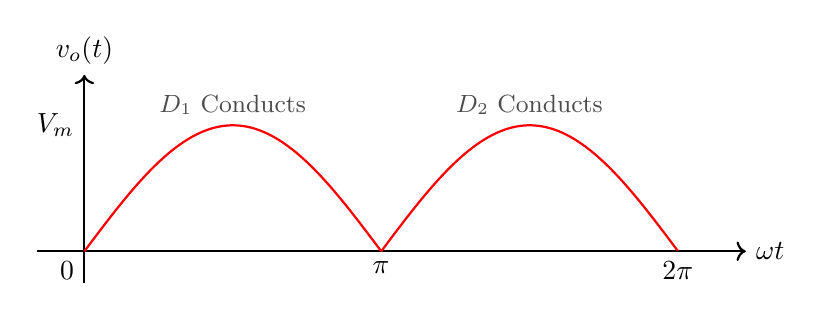
\begin{tikzpicture}[xscale=1.2, yscale=0.8]
        % Output DC Voltage Axes
        \draw[->, thick] (-0.5, 0) -- (7, 0) node[right] {$\omega t$};
        \draw[->, thick] (0, -0.5) -- (0, 2.8) node[above] {$v_o(t)$};
        
        % Full wave rectified output
        \draw[red, thick, domain=0:3.14, samples=100] plot (\x, {2*sin(\x r)});
        \draw[red, thick, domain=3.14:6.28, samples=100] plot (\x, {-2*sin(\x r)});
        
        % Output Labels
        \node[left] at (0, 2) {$V_m$};
        \node[below left] at (0, 0) {$0$};
        \node[below] at (3.14, 0) {$\pi$};
        \node[below] at (6.28, 0) {$2\pi$};
        
        % Conduction markers
        \node[above, text=black!70] at (1.57, 2) {\small $D_1$ Conducts};
        \node[above, text=black!70] at (4.71, 2) {\small $D_2$ Conducts};
    \end{tikzpicture}
\end{center}

\subsection*{3. Commentary on RC Time Constant in Rectifier Filter Circuits}

The raw output of a rectifier is pulsating DC, which is unsuitable for most electronic devices. To smooth out these pulsations, a filter capacitor ($C$) is placed in parallel with the load resistor ($R_L$). The effectiveness of this smoothing depends heavily on the \textbf{RC time constant ($\tau = R_L C$)}.

\begin{itemize}
    \item \textbf{Discharge Rate:} The time constant $\tau$ dictates how quickly the capacitor discharges through the load resistor when the input voltage falls below the capacitor's peak voltage. 
    \item \textbf{Requirement for Low Ripple:} To maintain a steady DC output, the capacitor must discharge very slowly relative to the frequency of the incoming pulses. Since a full-wave rectifier doubles the fundamental frequency ($f_{out} = 2f_{in}$), the time interval between peaks is $T/2$. Therefore, for good filtering, we require:
    \begin{equation}
        R_L C \gg \frac{T}{2} \quad \text{or} \quad R_L C \gg \frac{1}{2f_{in}}
    \end{equation}
    \item \textbf{Impact of Values:} 
    \begin{itemize}
        \item \textbf{Large RC ($\tau \gg T/2$):} The capacitor discharges minimally between peaks. The output voltage remains close to $V_m$, resulting in a \textit{small ripple voltage}. The peak-to-peak ripple voltage can be approximated as $V_{r(pp)} \approx \frac{V_m}{2 f_{in} R_L C}$.
        \item \textbf{Small RC ($\tau \approx T/2$):} The capacitor discharges significantly between peaks. The ripple voltage becomes large, and the average DC output voltage drops, degrading the performance of the power supply.
    \end{itemize}
\end{itemize}
In summary, a large RC time constant (using a large filter capacitor) is crucial in rectifier circuits to minimize voltage ripple and provide a smooth, stable DC supply.

\end{tcolorbox}

\item Draw the transfer curve of the circuit shown, assuming all diodes are ideal, $R_1=R_2=20\,\text{k}\Omega$, and $R_L=10\,\text{k}\Omega$. (i) What is the maximum peak voltage of the output signal? (ii) What is the peak-inverse voltage? (iii) What is the average current through the load?
\begin{center}
         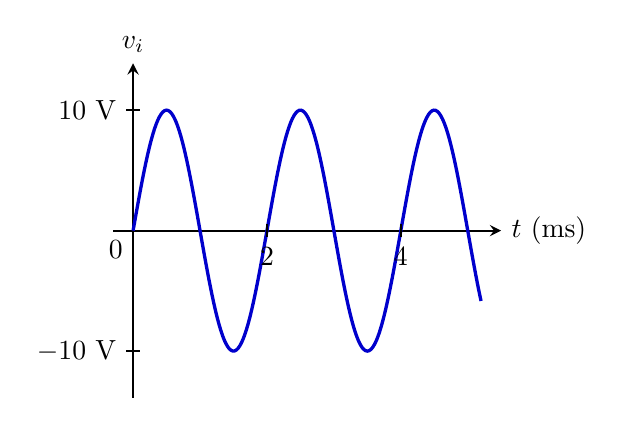
\begin{tikzpicture}[thick,scale=0.85, baseline=(current bounding box.center)]
            % Grid/Axes
            \draw[->, >=stealth, thick] (-0.3, 0) -- (5.5, 0) node[right] {$t\text{ (ms)}$};
            \draw[->, >=stealth, thick] (0, -2.5) -- (0, 2.5) node[above] {$v_i$};
            
            % Origin label
            \node[below left] at (0,0) {$0$};
            
            % Mathematical curve: Period = 2 units, Peak = 1.8 units
            % TikZ sin() expects degrees by default: \x*180 maps 1 unit to 180 degrees (half cycle)
            \draw[domain=0:5.2, samples=200, smooth, blue!80!black, very thick] 
                plot (\x, {1.8*sin(\x*180)});
            
            % X-axis ticks & labels
            \draw[thick] (2, 0.1) -- (2, -0.1) node[below] {$2$};
            \draw[thick] (4, 0.1) -- (4, -0.1) node[below] {$4$};
            
            % Y-axis ticks & labels
            \draw[thick] (0.1, 1.8) -- (-0.1, 1.8) node[left] {$10\text{ V}$};
            \draw[thick] (0.1, -1.8) -- (-0.1, -1.8) node[left] {$-10\text{ V}$};
        \end{tikzpicture}
\end{center}
\begin{center}

        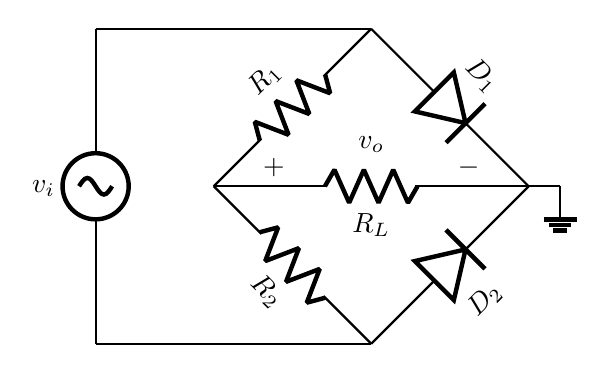
\begin{tikzpicture}[thick,scale=1.0, transform shape, baseline=(current bounding box.center)]
            % Bridge core nodes
            \coordinate (Top) at (2,2);
            \coordinate (Bottom) at (2,-2);
            \coordinate (Left) at (0,0);
            \coordinate (Right) at (4,0);
            
            % AC Voltage Source on the far left
            \draw (-1.5,-2) to[sinusoidal voltage source, l=$v_i$] (-1.5,2);
            
            % Source connections to bridge apexes
            \draw (-1.5,2) -- (Top);
            \draw (-1.5,-2) -- (Bottom);
            
            % Bridge Arms
            \draw (Top) to[R, l_=$R_1$] (Left);
            \draw (Left) to[R, l_=$R_2$] (Bottom);
            \draw (Top) to[D, l=$D_1$] (Right);
            \draw (Bottom) to[D, l_=$D_2$] (Right);
            
            % Center Load Resistor + Differential Voltage marker
            \draw (Left) to[R, l_=$R_L$, v^=$v_o$] (Right);
            
            % Ground Reference connection
            \draw (Right) -- (4.4,0) node[ground]{};
        \end{tikzpicture}

\end{center}
\mk{23} \yr{EEE 263 | L-2/T-1 | 2020--21}

\begin{tcolorbox}[enhanced,breakable,ansbox,colback=cA!4,colframe=cA,boxrule=0.8pt,arc=5pt,title={\textbf{Answer}},fonttitle=\bfseries\color{white},colbacktitle=cA]

\subsubsection*{1. Circuit Analysis and Operation}

\textbf{Given Parameters:}
\begin{itemize}
    \item Input voltage $v_i(t)$ is a sinusoid with a peak amplitude of $10\text{ V}$.
    \item $R_1 = R_2 = 20\text{ k}\Omega$
    \item $R_L = 10\text{ k}\Omega$
    \item Diodes $D_1$ and $D_2$ are ideal ($V_D = 0\text{ V}$).
\end{itemize}

\begin{center}
\begin{circuitikz}[american, thick,x=1.6cm,y=1.6cm, scale=1.0, transform shape]
    % Bridge core nodes
    \coordinate (Top) at (2,2);
    \coordinate (Bottom) at (2,-2);
    \coordinate (Left) at (0,0);
    \coordinate (Right) at (4,0);
    
    % AC Voltage Source on the far left
    \draw (-1.5,-2) to[sV, l=$v_i$] (-1.5,2);
    \node[right] at (-1.5, 1.5) {$+$};
    \node[right] at (-1.5, -1.5) {$-$};
    
    % Source connections to bridge apexes
    \draw (-1.5,2) -- (Top);
    \draw (-1.5,-2) -- (Bottom);
    
    % Bridge Arms
    \draw (Top) to[R, l=$R_1$, a=20\,k$\Omega$] (Left);
    \draw (Left) to[R, l=$R_2$, a=20\,k$\Omega$] (Bottom);
    \draw (Top) to[D, l=$D_1$] (Right);
    \draw (Bottom) to[D, l_=$D_2$] (Right);
    
    % Center Load Resistor + Differential Voltage marker
    \draw (Left) to[R, l_={$R_L=10\,k\Omega$}, v^=$v_o$] (Right);
    
    % Ground Reference connection
    \draw (Right) -- (4.4,0) node[ground]{};
    
    % Node labels
    \filldraw (Top) circle (1.5pt) node[above] {$V_{top}$};
    \filldraw (Bottom) circle (1.5pt) node[below] {$V_{bot}$};
    \filldraw (Left) circle (1.5pt) node[left] {$V_{left}$};
\end{circuitikz}
\end{center}


By standard convention, the sinusoidal source $v_i$ applies its voltage such that $v_i = V_{top} - V_{bot}$. The right node is grounded ($0\text{ V}$). Thus, the output voltage across the load is exactly the node voltage at the left node: $v_o = V_{left}$.

\textbf{Case 1: Positive Half-Cycle ($v_i > 0$)}
\begin{itemize}
    \item The potential at the top node is higher than the bottom node.
    \item Diode $D_1$ is forward-biased (ON) because its anode is pulled positive relative to ground. As $D_1$ is ideal, it acts as a short circuit, locking $V_{top} = 0\text{ V}$.
    \item Since $v_i = V_{top} - V_{bot}$, we have $V_{bot} = V_{top} - v_i = -v_i$.
    \item Diode $D_2$ is reverse-biased (OFF) because its anode is at $-v_i$ (negative) and its cathode is at $0\text{ V}$.
    \item Applying Kirchhoff's Current Law (KCL) at the $V_{left}$ node:
    \begin{align*}
        \frac{V_{left} - V_{top}}{R_1} + \frac{V_{left} - V_{bot}}{R_2} + \frac{V_{left} - 0}{R_L} &= 0 \\
        \frac{v_o - 0}{20\text{k}} + \frac{v_o - (-v_i)}{20\text{k}} + \frac{v_o}{10\text{k}} &= 0
    \end{align*}
    Multiplying the entire equation by $20\text{k}\Omega$:
    \begin{align*}
        v_o + (v_o + v_i) + 2v_o &= 0 \notag \\
        4v_o &= -v_i \notag \\
        v_o &= -0.25 v_i
    \end{align*}
\end{itemize}

\textbf{Case 2: Negative Half-Cycle ($v_i < 0$)}
\begin{itemize}
    \item The potential at the bottom node is higher than the top node.
    \item Diode $D_2$ is forward-biased (ON). Acting as a short, it locks $V_{bot} = 0\text{ V}$.
    \item Since $v_i = V_{top} - V_{bot}$, we have $V_{top} = v_i + V_{bot} = v_i$ (which is a negative value).
    \item Diode $D_1$ is reverse-biased (OFF) because its anode is at $v_i$ (negative) while its cathode is at $0\text{ V}$.
    \item Applying KCL at the $V_{left}$ node:
    \begin{align*}
        \frac{V_{left} - V_{top}}{R_1} + \frac{V_{left} - V_{bot}}{R_2} + \frac{V_{left} - 0}{R_L} &= 0 \\
        \frac{v_o - v_i}{20\text{k}} + \frac{v_o - 0}{20\text{k}} + \frac{v_o}{10\text{k}} &= 0
    \end{align*}
    Multiplying by $20\text{k}\Omega$:
    \begin{align*}
        (v_o - v_i) + v_o + 2v_o &= 0 \notag \\
        4v_o &= v_i \notag \\
        v_o &= 0.25 v_i
    \end{align*}
\end{itemize}

\textbf{General Transfer Function:} 
Combining both half-cycles, the output voltage is always negative and scaled by $0.25$. This defines an inverting full-wave rectifier:
\begin{equation}
    v_o = -0.25 |v_i|
\end{equation}

\vspace{1em}
\subsubsection*{2. Voltage Transfer Curve}
Based on the derived relationship $v_o = -0.25 |v_i|$, the transfer characteristic is plotted below:

\begin{center}
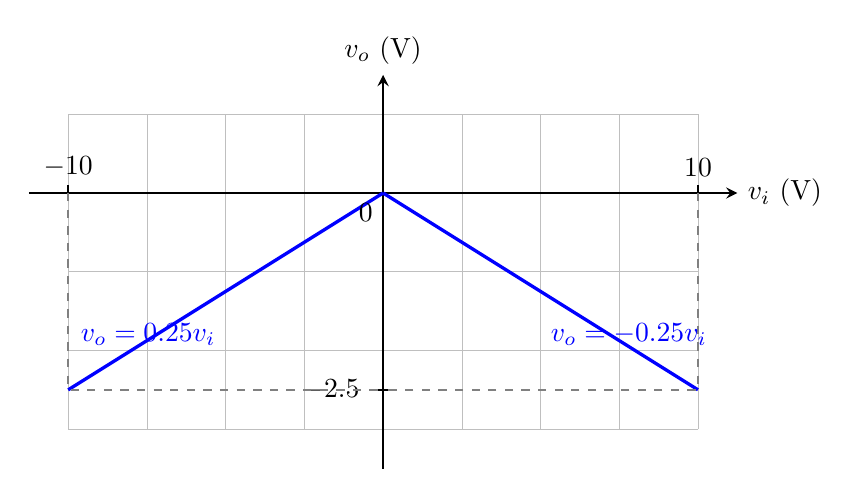
\begin{tikzpicture}[thick, scale=1.0]
    % Grid lines
    \draw[lightgray, very thin, step=1cm] (-4,-3) grid (4,1);
    
    % Axes
    \draw[->, >=stealth, thick] (-4.5, 0) -- (4.5, 0) node[right] {$v_i\text{ (V)}$};
    \draw[->, >=stealth, thick] (0, -3.5) -- (0, 1.5) node[above] {$v_o\text{ (V)}$};
    
    % Transfer Curve Plot (vo = -0.25 * |vi|)
    % Scaled for Tikz: x = vi / 2.5, y = vo
    % So vi=10 corresponds to x=4, vo=-2.5
    \draw[domain=0:4, samples=100, smooth, blue, very thick] plot (\x, {-0.25*(\x*2.5)});
    \draw[domain=-4:0, samples=100, smooth, blue, very thick] plot (\x, {0.25*(\x*2.5)});
    
    % Ticks and Labels
    \node[below left] at (0,0) {$0$};
    
    \draw[thick] (4, 0.1) -- (4, -0.1) node[above=5pt] {$10$};
    \draw[thick] (-4, 0.1) -- (-4, -0.1) node[above=5pt] {$-10$};
    
    \draw[thick] (0.1, -2.5) -- (-0.1, -2.5) node[left=2pt] {$-2.5$};
    
    % Dashed guidelines
    \draw[dashed, gray] (4, 0) -- (4, -2.5) -- (0, -2.5);
    \draw[dashed, gray] (-4, 0) -- (-4, -2.5) -- (0, -2.5);
    
    \node[blue, right] at (2, -1.8) {$v_o = -0.25 v_i$};
    \node[blue, left] at (-2, -1.8) {$v_o = 0.25 v_i$};
\end{tikzpicture}
\end{center}

\vspace{1em}
\subsubsection*{3. Answers to Specific Questions}

\textbf{(i) Maximum peak voltage of the output signal}
The input signal reaches a peak magnitude of $10\text{ V}$.
\begin{align*}
    V_{o(peak)} &= 0.25 \times V_{i(peak)} \notag \\
    &= 0.25 \times 10\text{ V} \notag \\
    &= \mathbf{2.5\text{ V}} \quad \text{(Amplitude reaches } -2.5\text{ V)}
\end{align*}

\textbf{(ii) Peak-Inverse Voltage (PIV)}
The PIV is the maximum reverse voltage across an OFF diode. During the positive half-cycle ($v_i = 10\text{ V}$), $D_1$ is ON (acting as a short, $V_{top} = 0\text{ V}$) and $D_2$ is OFF. The voltage at the bottom node is:
\begin{equation*}
    V_{bot} = -v_i = -10\text{ V}
\end{equation*}
The cathode of $D_2$ is grounded ($0\text{ V}$) and its anode is at $-10\text{ V}$. The reverse voltage across $D_2$ is:
\begin{equation}
    V_R = V_{cathode} - V_{anode} = 0\text{ V} - (-10\text{ V}) = \mathbf{10\text{ V}}
\end{equation}

\textbf{(iii) Average current through the load}
The output voltage $v_o(t)$ is a negative full-wave rectified sine wave with a peak of $2.5\text{ V}$. The DC (average) value of a full-wave rectified signal is:
\begin{equation}
    V_{o(avg)} = \frac{-2 V_{o(peak)}}{\pi} = \frac{-2(2.5\text{ V})}{\pi} = -\frac{5}{\pi}\text{ V} \approx -1.591\text{ V}
\end{equation}
The average current through the load resistor $R_L$ is:
\begin{equation}
    I_{L(avg)} = \frac{V_{o(avg)}}{R_L} = \frac{-1.591\text{ V}}{10\text{ k}\Omega} = \mathbf{-159.1\text{ }\mu\text{A}} \text{ (or } \mathbf{-0.159\text{ mA}}\text{)}
\end{equation}
\textit{Note: The negative sign indicates that the actual average current flows from right to left (from ground, through $R_L$, to the $V_{left}$ node).}

\vspace{1em}
\subsubsection*{4. Final Summary Table}
\begin{center}
\renewcommand{\arraystretch}{1.5}
\begin{tabular}{@{}llc@{}}
\toprule
\textbf{Parameter} & \textbf{Symbol} & \textbf{Calculated Value} \\ \midrule
(i) Maximum Peak Output Voltage & $V_{o(peak)}$ & $2.5\text{ V}$ \\
(ii) Peak-Inverse Voltage & $\text{PIV}$ & $10\text{ V}$ \\
(iii) Average Load Current & $I_{L(avg)}$ & $-0.159\text{ mA}$ \\ \bottomrule
\end{tabular}
\end{center}

\end{tcolorbox}

\item Draw the circuit of a full-wave bridge rectifier and show the output wave shape for a sinusoidal input.
\mk{16} \yr{EEE 263 | L-2/T-1 | 2018--19}

\begin{tcolorbox}[enhanced,breakable,ansbox,colback=cA!4,colframe=cA,boxrule=0.8pt,arc=5pt,title={\textbf{Answer}},fonttitle=\bfseries\color{white},colbacktitle=cA]

\subsubsection*{1. Full-Wave Bridge Rectifier Circuit Diagram}
The full-wave bridge rectifier utilizes four diodes arranged in a bridge configuration to convert the entire AC input cycle (both positive and negative half-cycles) into pulsating DC output.
\begin{center}
\begin{circuitikz}[american, thick, scale=0.9, transform shape]
    % AC Source
    \draw (0,2) to[sV, l=$v_i(t)$] (0,-2.5);
    
    % Bridge Nodes
    \coordinate (C) at (2, 0);   % Left (AC input)
    \coordinate (D) at (6, 0);   % Right (AC input)
    \coordinate (A) at (4, 2);   % Top (DC output +)
    \coordinate (B) at (4, -2);  % Bottom (DC output -)
    
    % Connections from Source to Bridge
    \draw (0,2) -- (2,2) -- (C);
    \draw (0,-2.5) -| (D);
    
    % Diodes
    \draw (C) to[D, l=$D_1$] (A);
    \draw (B) to[D, l=$D_2$] (C);
    \draw (D) to[D, l_=$D_3$] (A);
    \draw (B) to[D, l_=$D_4$] (D);
    
    % Load Network
    \draw (A) -- (4, 3) -- (8.5, 3);
    \draw (B) -- (4, -3) -- (8.5, -3);
    \draw (8.5, 3) to[R, l=$R_L$, v=$v_o(t)$] (8.5, -3);
    
    % Ground Connection
    \draw (8.5, -3) node[ground]{};
    
    % Node Labels
    \filldraw (C) circle (2pt);
    \filldraw (D) circle (2pt);
    \filldraw (A) circle (2pt);
    \filldraw (B) circle (2pt);
\end{circuitikz}
\end{center}


\vspace{1em}
\subsubsection*{2. Input and Output Wave Shapes}
Assuming a practical diode model where each diode has a forward voltage drop $V_D$ (typically $0.7\text{ V}$ for silicon), the peak output voltage is reduced by $2V_D$ because two diodes conduct simultaneously in series during any half-cycle.

\begin{center}
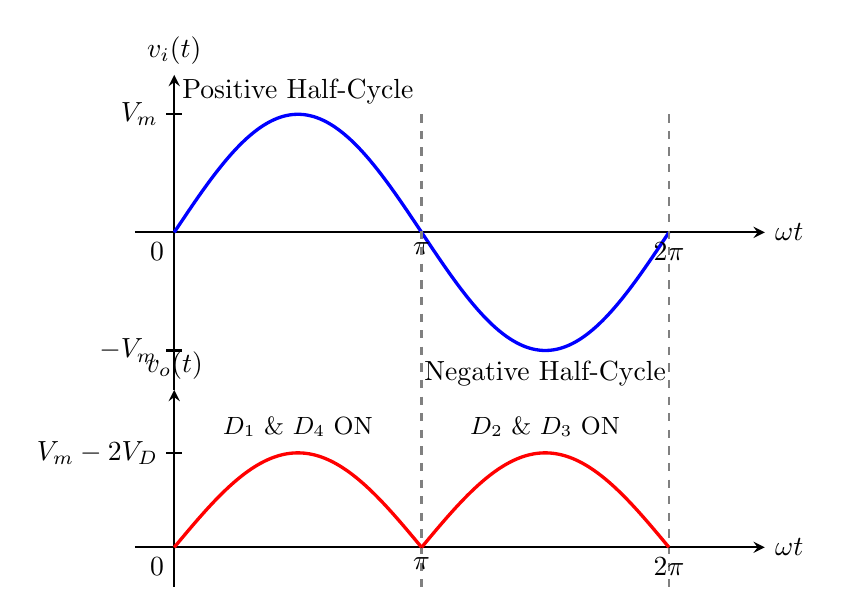
\begin{tikzpicture}[thick, scale=1.0, transform shape]
    % ---------------- INPUT WAVEFORM ---------------- %
    \begin{scope}[shift={(0,4)}]
        % Axes
        \draw[->, >=stealth] (-0.5, 0) -- (7.5, 0) node[right] {$\omega t$};
        \draw[->, >=stealth] (0, -2) -- (0, 2) node[above] {$v_i(t)$};
        
        % Sine Wave
        \draw[domain=0:2*pi, samples=150, smooth, blue, very thick] plot (\x, {1.5*sin(\x*180/pi)});
        
        % Labels & Ticks
        \draw (-0.1, 1.5) -- (0.1, 1.5) node[left=5pt] {$V_m$};
        \draw (-0.1, -1.5) -- (0.1, -1.5) node[left=5pt] {$-V_m$};
        \node[below left] at (0,0) {$0$};
        \node[below] at (pi, 0) {$\pi$};
        \node[below] at (2*pi, 0) {$2\pi$};
        
        % Alignment lines
        \draw[dashed, gray] (pi, 1.5) -- (pi, -4.5);
        \draw[dashed, gray] (2*pi, 1.5) -- (2*pi, -4.5);
        \node[above] at (1.57, 1.5) {Positive Half-Cycle};
        \node[below] at (4.71, -1.5) {Negative Half-Cycle};
    \end{scope}
    
    % ---------------- OUTPUT WAVEFORM ---------------- %
    \begin{scope}[shift={(0,0)}]
        % Axes
        \draw[->, >=stealth] (-0.5, 0) -- (7.5, 0) node[right] {$\omega t$};
        \draw[->, >=stealth] (0, -0.5) -- (0, 2) node[above] {$v_o(t)$};
        
        % Rectified Sine Wave (Positive Half)
        \draw[domain=0:pi, samples=100, smooth, red, very thick] plot (\x, {1.2*sin(\x*180/pi)});
        % Rectified Sine Wave (Negative Half flipped)
        \draw[domain=pi:2*pi, samples=100, smooth, red, very thick] plot (\x, {-1.2*sin(\x*180/pi)});
        
        % Labels & Ticks
        \draw (-0.1, 1.2) -- (0.1, 1.2) node[left=5pt] {$V_m - 2V_D$};
        \node[below left] at (0,0) {$0$};
        \node[below] at (pi, 0) {$\pi$};
        \node[below] at (2*pi, 0) {$2\pi$};
        
        % Conduction State Labels
        \node[above=2pt, font=\small, text=black] at (1.57, 1.2) {$D_1$ \& $D_4$ ON};
        \node[above=2pt, font=\small, text=black] at (4.71, 1.2) {$D_2$ \& $D_3$ ON};
    \end{scope}
\end{tikzpicture}
\end{center}

\vspace{0.5em}
\textbf{Summary of Operation:}
\begin{itemize}
    \item \textbf{Positive Half-Cycle ($0 \to \pi$):} The top of the AC source is positive. Current flows through $D_1$, down through the load resistor $R_L$, and returns to the source through $D_4$. Diodes $D_2$ and $D_3$ are reverse-biased.
    \item \textbf{Negative Half-Cycle ($\pi \to 2\pi$):} The bottom of the AC source is positive. Current flows through $D_3$, down through the load resistor $R_L$ (in the \textit{same} direction as before), and returns to the source through $D_2$. Diodes $D_1$ and $D_4$ are reverse-biased.
\end{itemize}

\end{tcolorbox}

\item For a full-wave bridge rectifier, find the value of peak current through the diode and PIV for the diode. Given: $V_s=12\,\text{V}$ (rms), $V_{DO}=0.7\,\text{V}$, $R=100\,\Omega$.
\mk{10} \yr{EEE 263 | L-2/T-1 | 2018--19}

\begin{tcolorbox}[enhanced,breakable,ansbox,colback=cA!4,colframe=cA,boxrule=0.8pt,arc=5pt,title={\textbf{Answer}},fonttitle=\bfseries\color{white},colbacktitle=cA]

\subsubsection*{1. Given Parameters}
\begin{itemize}
    \item RMS Input Voltage, $V_{s(rms)} = 12\text{ V}$
    \item Diode Forward Voltage Drop, $V_{DO} = 0.7\text{ V}$
    \item Load Resistance, $R = 100\,\Omega$
\end{itemize}

\vspace{1em}
\subsubsection*{2. Mathematical Derivations}

\textbf{Step 2.1: Peak Source Voltage ($V_{s(peak)}$)}
The peak voltage of the AC source is calculated by multiplying the RMS voltage by $\sqrt{2}$:
\begin{equation}
    V_{s(peak)} = \sqrt{2} \times V_{s(rms)} = \sqrt{2} \times 12\text{ V} \approx 16.97\text{ V}
\end{equation}

\vspace{0.5em}
\textbf{Step 2.2: Peak Output Voltage ($V_{o(peak)}$)}
In a full-wave bridge rectifier, two diodes conduct in series during each half-cycle. Therefore, the peak voltage reaching the load resistor $R$ is the peak source voltage minus the voltage drop of two forward-biased diodes:
\begin{align*}
    V_{o(peak)} &= V_{s(peak)} - 2V_{DO} \notag \\
    &= 16.97\text{ V} - 2(0.7\text{ V}) \notag \\
    &= 16.97\text{ V} - 1.4\text{ V} = \mathbf{15.57\text{ V}}
\end{align*}

\vspace{0.5em}
\textbf{Step 2.3: Peak Diode Current ($I_{peak}$)}
During conduction, the peak current flowing through the series pair of diodes is equivalent to the peak current through the load resistor. Applying Ohm's Law:
\begin{align*}
    I_{peak} &= \frac{V_{o(peak)}}{R} \notag \\
    &= \frac{15.57\text{ V}}{100\,\Omega} \notag \\
    &= 0.1557\text{ A} = \mathbf{155.7\text{ mA}}
\end{align*}

\vspace{0.5em}
\textbf{Step 2.4: Peak Inverse Voltage (PIV)}
The Peak Inverse Voltage is the maximum reverse voltage a diode must withstand when it is non-conducting. In a bridge rectifier, a non-conducting diode is in parallel with the secondary source and one forward-biased diode. Applying Kirchhoff's Voltage Law (KVL):
\begin{align*}
    \text{PIV} &= V_{s(peak)} - V_{DO} \notag \\
    &= 16.97\text{ V} - 0.7\text{ V} = \mathbf{16.27\text{ V}}
\end{align*}

\vspace{1em}
\subsubsection*{3. Final Answer Summary}
\begin{center}
\renewcommand{\arraystretch}{1.5}
\begin{tabular}{@{}llc@{}}
\toprule
\textbf{Parameter} & \textbf{Symbol} & \textbf{Calculated Value} \\ \midrule
Peak Source Voltage & $V_{s(peak)}$ & $16.97\text{ V}$ \\
Peak Diode Current & $I_{peak}$ & $155.7\text{ mA}$ \\
Peak Inverse Voltage & $\text{PIV}$ & $16.27\text{ V}$ \\ \bottomrule
\end{tabular}
\end{center}

\end{tcolorbox}

\item Comment on the value of RC time constant for a rectifier circuit.
\mk{10} \yr{EEE 263 | L-2/T-1 | 2018--19}

\begin{tcolorbox}[enhanced,breakable,ansbox,colback=cA!4,colframe=cA,boxrule=0.8pt,arc=5pt,title={\textbf{Answer}},fonttitle=\bfseries\color{white},colbacktitle=cA]

\subsubsection*{1. Introduction and Circuit Principle}
In a rectifier circuit, an output filter is almost always required to convert the pulsating DC voltage into a steady, constant DC voltage suitable for electronic loads. The most common and economical filtering method is placing a shunt capacitor ($C$) in parallel with the load resistor ($R_L$).

The behavior and effectiveness of this filter are heavily dependent on the \textbf{RC time constant ($\tau = R_L C$)}, which dictates the rate at which the capacitor discharges through the load when the rectifier diodes are not conducting.

\begin{center}
\begin{circuitikz}[thick]
    
    % AC Source (Transformer Secondary)
    \draw (0,0) to[sV] (0,-4);
    
    % AC Routing to Bridge Rectifier
    % Top AC line to left node of the bridge
    \draw (0,0) -- (1.5,0) -- (1.5,-2) -- (3,-2);
    % Bottom AC line to right node of the bridge (routed completely around)
    \draw (0,-4) -- (1.5,-4) -- (1.5,-6) -- (8,-6) -- (8,-2) -- (7,-2);
    
    % Bridge Rectifier Diodes
    \draw (3,-2) to[D, l=$D_1$] (5,0);
    \draw (7,-2) to[D, l_=$D_2$] (5,0);
    \draw (5,-4) to[D, l=$D_3$] (3,-2);
    \draw (5,-4) to[D, l_=$D_4$] (7,-2);
    
    % Bridge Connection Nodes
    \node[circ] at (3,-2) {};
    \node[circ] at (7,-2) {};
    \node[circ] at (5,0) {};
    \node[circ] at (5,-4) {};
    
    % DC Rails
    \draw (5,0) -- (13,0);
    \draw (5,-4) -- (13,-4);
    
    % Filter Capacitor
    \draw (10,0) to[C, l=$C$, *-*] (10,-4);
    
    % Ground (centered between C and R)
    \draw (11.5,-4) to[short, *-] (11.5,-4.5) node[ground]{};
    
    % Load Resistor
    \draw (13,0) to[R, l={$R$}] (13,-4);

\end{circuitikz}

\end{center}

\vspace{1em}
\subsubsection*{2. The Golden Rule of the RC Time Constant}
To effectively smooth the output voltage, the capacitor must discharge very slowly relative to the frequency of the incoming AC signal. The fundamental design criterion for the time constant is:
\begin{equation}
    \tau = R_L C \gg T
\end{equation}
where $T$ is the period of the rectified signal.
\begin{itemize}
    \item For a \textbf{Half-Wave Rectifier}: $T = \frac{1}{f_{in}}$. Thus, $R_L C \gg \frac{1}{f_{in}}$
    \item For a \textbf{Full-Wave Rectifier}: The rectified signal frequency is twice the input frequency ($2f_{in}$), so the effective period is $T = \frac{1}{2f_{in}}$. Thus, $R_L C \gg \frac{1}{2f_{in}}$
\end{itemize}

\vspace{1em}
\subsubsection*{3. Mathematical Relationship to Ripple Voltage}
The primary goal of selecting an appropriate RC time constant is to minimize the peak-to-peak ripple voltage ($V_r$). Assuming a linear discharge (valid when $R_L C \gg T$), the ripple voltage for a full-wave rectifier is approximated as:
\begin{equation}
    V_r \approx \frac{V_{peak}}{2 f_{in} R_L C}
\end{equation}
where $V_{peak}$ is the peak rectified voltage. This equation demonstrates that the ripple voltage is \textbf{inversely proportional} to the RC time constant.

\vspace{1em}
\subsubsection*{4. Design Trade-offs: Choosing the Value of $\tau$}

While the equation suggests making the RC time constant as large as possible to eliminate ripple, doing so introduces severe practical trade-offs. The selection of the RC value requires balancing DC quality against component stress.

\begin{center}
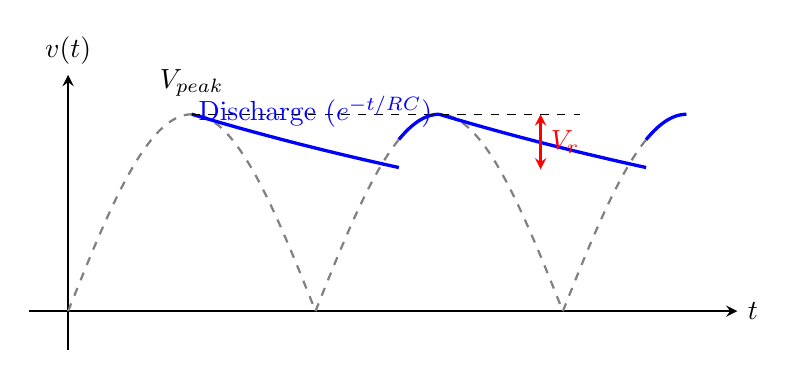
\begin{tikzpicture}[thick, scale=1.0, transform shape]
    % Axes
    \draw[->, >=stealth] (-0.5, 0) -- (8.5, 0) node[right] {$t$};
    \draw[->, >=stealth] (0, -0.5) -- (0, 3) node[above] {$v(t)$};
    
    % Rectified Sine Waves (dashed for reference)
    \draw[domain=0:pi, samples=100, smooth, gray, dashed] plot (\x, {2.5*sin(\x*180/pi)});
    \draw[domain=pi:2*pi, samples=100, smooth, gray, dashed] plot (\x, {-2.5*sin(\x*180/pi)});
    \draw[domain=2*pi:2.5*pi, samples=50, smooth, gray, dashed] plot (\x, {2.5*sin(\x*180/pi)});
    
    % Filtered Output (Blue)
    % Peak at pi/2 (1.57). Next peak at 3pi/2 (4.71)
    \draw[domain=1.57:4.2, samples=100, smooth, blue, very thick] plot (\x, {2.5*exp(-0.12*(\x-1.57))});
    \draw[domain=4.2:4.71, samples=50, smooth, blue, very thick] plot (\x, {-2.5*sin(\x*180/pi)});
    
    \draw[domain=4.71:7.34, samples=100, smooth, blue, very thick] plot (\x, {2.5*exp(-0.12*(\x-4.71))});
    \draw[domain=7.34:7.85, samples=50, smooth, blue, very thick] plot (\x, {2.5*sin(\x*180/pi)});
    
    % Ripple markers
    \draw[<->, >=stealth, red] (6.0, 2.5) -- (6.0, 1.8) node[midway, right] {$V_r$};
    \draw[dashed, thin, black] (1.57, 2.5) -- (6.5, 2.5);
    
    % Labels
    \node[blue, above] at (3.14, 2.2) {Discharge ($e^{-t/RC}$)};
    \node[above] at (1.57, 2.6) {$V_{peak}$};
\end{tikzpicture}
\end{center}

\textbf{Case 1: Very Large RC Time Constant (Large $C$ or Large $R_L$)}
\begin{itemize}
    \item \textbf{Advantage (Low Ripple):} The capacitor discharges very slowly between peaks. The output DC voltage is smooth, and the average DC level remains very close to $V_{peak}$.
    \item \textbf{Disadvantage (High Surge Current):} Because the capacitor voltage remains high, the incoming AC sine wave only exceeds the capacitor voltage for a very brief interval near the peak. The diodes only conduct during this tiny window (narrow conduction angle). To supply the required average load current, the diodes must pass massive, short-duration spikes of \textit{surge current}, which can exceed their peak repetitive forward current ($I_{FRM}$) rating and destroy them.
\end{itemize}

\textbf{Case 2: Small RC Time Constant (Small $C$ or Small $R_L$)}
\begin{itemize}
    \item \textbf{Disadvantage (High Ripple):} The capacitor discharges deeply between peaks. The output exhibits a large "sawtooth" ripple, and the average DC voltage drops significantly. This poor regulation is unacceptable for sensitive analog circuits.
    \item \textbf{Advantage (Lower Peak Diode Current):} The capacitor voltage drops lower, meaning the AC source voltage exceeds it earlier in the cycle. The conduction angle increases, spreading the charging current over a longer time and reducing the peak thermal stress on the diodes.
\end{itemize}

\vspace{0.5em}
\textbf{Conclusion:}
The value of the RC time constant must be chosen as a compromise. It should be large enough to keep the ripple voltage within the tolerance required by the load (or the subsequent voltage regulator), but it must not be so excessively large that it causes the peak repetitive diode currents to exceed safe operating limits.

\end{tcolorbox}

\item Draw the circuit diagram of a full wave rectifier with a filter capacitor. Assume the input is a sinusoidal signal with 10\,kHz frequency and 7.07\,V rms voltage, the load is 1\,k$\Omega$ and capacitor used is 1\,$\mu$F. Diode has a forward voltage drop of 0.7\,V. Find:
\begin{enumerate}
  \item Ripple voltage.
  \item PIV and duty cycle.
  \item Peak output voltage.
\end{enumerate}
\mk{16} \yr{EEE 263 | L-2/T-1 | 2015--16}

\begin{tcolorbox}[enhanced,breakable,ansbox,colback=cA!4,colframe=cA,boxrule=0.8pt,arc=5pt,title={\textbf{Answer}},fonttitle=\bfseries\color{white},colbacktitle=cA]

\subsection*{1. Circuit Diagram}

\textbf{Assumption:} As no transformer is explicitly specified, a \textbf{Full-Wave Bridge Rectifier} topology is assumed. This requires two diode voltage drops ($2V_D$) per half-cycle conduction path.

\begin{center}
    \begin{circuitikz}[thick, scale=1.0, transform shape]
        % Bridge nodes
        \coordinate (AC1) at (0,0);
        \coordinate (DC+) at (2,2);
        \coordinate (AC2) at (4,0);
        \coordinate (DC-) at (2,-2);
        
        % Diodes in Bridge
        \draw (AC1) to[D, l=$D_1$] (DC+);
        \draw (AC2) to[D, l_=$D_2$] (DC+);
        \draw (DC-) to[D, l=$D_3$] (AC1);
        \draw (DC-) to[D, l_=$D_4$] (AC2);
        
        % Dots at bridge junctions
        \fill (AC1) circle (2pt);
        \fill (AC2) circle (2pt);
        \fill (DC+) circle (2pt);
        \fill (DC-) circle (2pt);
        
        % AC Input Source
        \draw (-2.5,0) to[sV, l=$v_{in}$] (-2.5,-4) -- (4,-4) -- (AC2);
        \draw (-2.5,0) -- (AC1);
        \node[anchor=south] at (-2.5, 0.8) {$7.07\,\mathrm{V_{rms}}$};
        \node[anchor=north] at (-2.5, -0.8) {$10\,\mathrm{kHz}$};
        
        % DC Output Stage
        \draw (DC+) -- (7,2);
        \draw (DC-) -- (7,-2);
        
        % Filter Capacitor and Load
        \draw (5,2) to[C, l=$C{=}1\,\mu\mathrm{F}$] (5,-2);
        \draw (7,2) to[R, l=$R_L{=}1\,\mathrm{k}\Omega$] (7,-2);
        
        % Junction dots for C and R
        \fill (5,2) circle (2pt);
        \fill (5,-2) circle (2pt);
        \fill (7,2) circle (2pt);
        
        % Ground connections
        \draw (DC-) node[ground]{};
        \draw (7,-2) node[ground]{};
        
        % Output Voltage Labels
        \draw[->, >=stealth] (7.8, 1.8) -- (7.8, -1.8) node[midway, right] {$v_{out}$};
        \node at (7.8, 2.1) {$+$};
        \node at (7.8, -2.1) {$-$};
    \end{circuitikz}
\end{center}

\subsection*{2. Given Parameters}
\begin{itemize}
    \item RMS Input Voltage, $V_{rms} = 7.07\,\mathrm{V}$
    \item Input Frequency, $f = 10\,\mathrm{kHz}$
    \item Load Resistance, $R_L = 1\,\mathrm{k}\Omega = 1000\,\Omega$
    \item Filter Capacitance, $C = 1\,\mu\mathrm{F} = 10^{-6}\,\mathrm{F}$
    \item Diode Forward Drop, $V_D = 0.7\,\mathrm{V}$
\end{itemize}

\subsection*{3. Mathematical Derivations and Solutions}

\textbf{Step 3a: Peak Input Voltage}\\
The peak value of the input sinusoidal voltage is:
\begin{equation}
    V_{in(peak)} = V_{rms} \times \sqrt{2} = 7.07\,\mathrm{V} \times 1.414 \approx 10.0\,\mathrm{V}
\end{equation}

\textbf{Step 3b: Peak Output Voltage ($V_{p,out}$)}\\
In a bridge rectifier, the current flows through two diodes simultaneously during each half-cycle. Therefore, the peak output voltage is the peak input voltage minus two diode drops:
\begin{align*}
    V_{p,out} &= V_{in(peak)} - 2V_D \nonumber \\
    &= 10.0\,\mathrm{V} - 2(0.7\,\mathrm{V}) \nonumber \\
    &= 10.0\,\mathrm{V} - 1.4\,\mathrm{V} \nonumber \\
    &= 8.6\,\mathrm{V}
\end{align*}

\textbf{Step 3c: Ripple Voltage ($V_r$)}\\
For a full-wave rectifier, the ripple frequency is twice the input frequency ($f_r = 2f = 20\,\mathrm{kHz}$). The peak-to-peak ripple voltage $V_{r(pp)}$ is approximated by:
\begin{align*}
    V_{r(pp)} &\approx \frac{V_{p,out}}{f_r R_L C} = \frac{V_{p,out}}{2 f R_L C} \nonumber \\
    &= \frac{8.6\,\mathrm{V}}{(2 \times 10^4\,\mathrm{Hz}) \times (10^3\,\Omega) \times (10^{-6}\,\mathrm{F})} \nonumber \\
    &= \frac{8.6}{20} \nonumber \\
    &= 0.43\,\mathrm{V}
\end{align*}

\textbf{Step 3d: Peak Inverse Voltage (PIV)}\\
In a bridge configuration, the maximum reverse voltage across any non-conducting diode is the peak input voltage minus the voltage drop of the conducting diode in its loop:
\begin{align*}
    \mathrm{PIV} &= V_{in(peak)} - V_D \nonumber \\
    &= 10.0\,\mathrm{V} - 0.7\,\mathrm{V} \nonumber \\
    &= 9.3\,\mathrm{V}
\end{align*}

\textbf{Step 3e: Duty Cycle}\\
The conduction angle $\theta_c$ (in radians) represents the small portion of the cycle where the diodes turn ON to recharge the capacitor. It is given by:
\begin{align*}
    \theta_c &\approx \sqrt{\frac{2 V_{r(pp)}}{V_{p,out}}} \nonumber \\
    &= \sqrt{\frac{2(0.43\,\mathrm{V})}{8.6\,\mathrm{V}}} = \sqrt{\frac{0.86}{8.6}} = \sqrt{0.1} \nonumber \\
    &\approx 0.3162\,\mathrm{rad}
\end{align*}
The duty cycle for an individual diode (which conducts once per full cycle of $2\pi$) is:
\begin{align*}
    \text{Duty Cycle (Diode)} &= \left( \frac{\theta_c}{2\pi} \right) \times 100\% \nonumber \\
    &= \left( \frac{0.3162}{2 \times 3.1416} \right) \times 100\% \nonumber \\
    &\approx 5.03\%
\end{align*}
\textit{Note: The overall rectifier circuit charges the capacitor twice per cycle, yielding an effective circuit duty cycle of $2 \times 5.03\% \approx 10.06\%$.}

\subsection*{4. Final Answer Summary}
\begin{center}
    \renewcommand{\arraystretch}{1.5}
    \begin{tabular}{@{}ll@{}}
        \toprule
        \textbf{Parameter} & \textbf{Calculated Value} \\
        \midrule
        Peak Output Voltage & $\mathbf{8.6\,\mathrm{V}}$ \\
        Ripple Voltage (Peak-to-Peak) & $\mathbf{0.43\,\mathrm{V}}$ \\
        Peak Inverse Voltage (PIV) & $\mathbf{9.3\,\mathrm{V}}$ \\
        Duty Cycle (per Diode) & $\mathbf{5.03\%}$ \\
        \bottomrule
    \end{tabular}
\end{center}

\end{tcolorbox}

\item Show that the average output voltage of a bridge rectifier circuit is $V_o = \frac{2}{\pi}V_s - 2V_{DO}$. If the input voltage is a 12\,V (rms) sinusoid and the load resistance is 100\,$\Omega$, calculate: (i) the average output voltage, (ii) the peak diode current, and (iii) the PIV of the diodes. Assume $V_{DO}=0.7\,\text{V}$.
\mk{16} \yr{EEE 263 | L-2/T-1 | 2011--12}

\begin{tcolorbox}[enhanced,breakable,ansbox,colback=cA!4,colframe=cA,boxrule=0.8pt,arc=5pt,title={\textbf{Answer}},fonttitle=\bfseries\color{white},colbacktitle=cA]

\subsubsection*{1. Reference Circuit Diagram}

\begin{center}
\begin{circuitikz}[american, thick, scale=0.9, transform shape]
    % AC Source
    \draw (0,2) to[sV, l=$v_i(t)$] (0,-2.5);
    
    % Bridge Nodes
    \coordinate (C) at (2, 0);   % Left (AC input)
    \coordinate (D) at (6, 0);   % Right (AC input)
    \coordinate (A) at (4, 2);   % Top (DC output +)
    \coordinate (B) at (4, -2);  % Bottom (DC output -)
    
    % Connections from Source to Bridge
    \draw (0,2) -- (2,2) -- (C);
    \draw (0,-2.5) -| (D);
    
    % Diodes
    \draw (C) to[D, l=$D_1$] (A);
    \draw (B) to[D, l=$D_2$] (C);
    \draw (D) to[D, l_=$D_3$] (A);
    \draw (B) to[D, l_=$D_4$] (D);
    
    % Load Network
    \draw (A) -- (4, 3) -- (8.5, 3);
    \draw (B) -- (4, -3) -- (8.5, -3);
    \draw (8.5, 3) to[R, l=$R_L$, v=$v_o(t)$] (8.5, -3);
    
    % Ground Connection
    \draw (8.5, -3) node[ground]{};
    
    % Node Labels
    \filldraw (C) circle (2pt);
    \filldraw (D) circle (2pt);
    \filldraw (A) circle (2pt);
    \filldraw (B) circle (2pt);
\end{circuitikz}
\end{center}

\vspace{1em}
\subsubsection*{2. Derivation of the Average Output Voltage Equation}

\textbf{Circuit Operation \& Assumption:}
Let the input voltage be a purely sinusoidal wave defined as $v_s(t) = V_s \sin(\omega t)$, where $V_s$ is the \textbf{peak} amplitude of the source. 
During the positive half-cycle, diodes $D_1$ and $D_4$ are forward-biased (ON). Assuming a constant voltage drop model, each conducting diode has a forward voltage drop of $V_{DO}$. 
Applying Kirchhoff's Voltage Law (KVL) around the conduction loop yields the instantaneous output voltage:
\begin{equation}
    v_o(t) = |v_s(t)| - 2V_{DO}
\end{equation}

\textbf{Mathematical Derivation:}
The average (DC) value of a periodic waveform is found by integrating it over one period and dividing by the period. For a full-wave rectified signal, the period is $\pi$. 
\begin{equation}
    V_o = \frac{1}{\pi} \int_{0}^{\pi} v_o(t) d(\omega t)
\end{equation}
Substituting the instantaneous voltage equation:
\begin{equation}
    V_o = \frac{1}{\pi} \int_{0}^{\pi} (V_s \sin(\omega t) - 2V_{DO}) d(\omega t)
\end{equation}
\textit{Note: This standard derivation neglects the small dead-band near the zero-crossings where the source voltage is less than $2V_{DO}$. We assume conduction occurs from $0$ to $\pi$.}

Splitting the integral:
\begin{equation}
    V_o = \frac{V_s}{\pi} \int_{0}^{\pi} \sin(\omega t) d(\omega t) - \frac{2V_{DO}}{\pi} \int_{0}^{\pi} d(\omega t)
\end{equation}
Evaluating the integrals:
\begin{align*}
    \int_{0}^{\pi} \sin(\omega t) d(\omega t) &= [-\cos(\omega t)]_0^\pi = -(-1) - (-1) = 2 \\
    \int_{0}^{\pi} d(\omega t) &= [\omega t]_0^\pi = \pi
\end{align*}
Substituting these results back into the equation yields the required expression:
\begin{align*}
    V_o &= \frac{V_s}{\pi} (2) - \frac{2V_{DO}}{\pi} (\pi) \notag \\
    V_o &= \mathbf{\frac{2}{\pi}V_s - 2V_{DO}}
\end{align*}

\vspace{1em}
\subsubsection*{3. Step-by-Step Calculations}

\textbf{Given Parameters:}
\begin{itemize}
    \item Input RMS Voltage, $V_{rms} = \textbf{12 V}$
    \item Load Resistance, $R = \textbf{100 } \Omega$
    \item Diode Forward Voltage, $V_{DO} = \textbf{0.7 V}$
\end{itemize}

First, we determine the \textbf{peak} source voltage ($V_s$), which is required for the formulas:
\begin{equation}
    V_s = \sqrt{2} \times V_{rms} = \sqrt{2} \times 12 = \mathbf{16.97\text{ V}}
\end{equation}

\vspace{0.5em}
\textbf{(i) Average Output Voltage ($V_o$)}
Using the derived equation:
\begin{align*}
    V_o &= \frac{2}{\pi}(16.97\text{ V}) - 2(0.7\text{ V}) \notag \\
    &= 10.80\text{ V} - 1.4\text{ V} \notag \\
    &= \mathbf{9.40\text{ V}}
\end{align*}

\vspace{0.5em}
\textbf{(ii) Peak Diode Current ($I_{peak}$)}
The peak diode current is equal to the peak load current. The peak voltage across the load occurs at the peak of the input cycle minus the two diode drops.
\begin{align*}
    V_{o(peak)} &= V_s - 2V_{DO} \notag \\
    &= 16.97\text{ V} - 1.4\text{ V} = 15.57\text{ V}
\end{align*}
Applying Ohm's Law to the load resistor:
\begin{align*}
    I_{peak} &= \frac{V_{o(peak)}}{R} \notag \\
    &= \frac{15.57\text{ V}}{100\text{ }\Omega} \notag \\
    &= 0.1557\text{ A} = \mathbf{155.7\text{ mA}}
\end{align*}

\vspace{0.5em}
\textbf{(iii) Peak Inverse Voltage (PIV)}
The PIV is the maximum reverse voltage across an OFF diode. In a bridge rectifier, the non-conducting diode is in parallel with the secondary source and one forward-biased diode.
\begin{align*}
    \text{PIV} &= V_s - V_{DO} \notag \\
    &= 16.97\text{ V} - 0.7\text{ V} \notag \\
    &= \mathbf{16.27\text{ V}}
\end{align*}

\vspace{1em}
\subsubsection*{4. Final Summary Table}
\begin{center}
\renewcommand{\arraystretch}{1.5}
\begin{tabular}{@{}llc@{}}
\toprule
\textbf{Parameter} & \textbf{Symbol} & \textbf{Calculated Value} \\ \midrule
(i) Average Output Voltage & $V_o$ & \textbf{9.40 V} \\
(ii) Peak Diode Current & $I_{peak}$ & \textbf{155.7 mA} \\
(iii) Peak Inverse Voltage & \text{PIV} & \textbf{16.27 V} \\ \bottomrule
\end{tabular}
\end{center}

\end{tcolorbox}

\end{enumerate}

%%──────────────────────────────────────────────────────────────────────
\subtopic{cA}{Zener Diode Regulator}
\label{sub:s1-zener}

\begin{enumerate}
    
\item A 6.8\,V Zener diode exhibits its nominal voltage at a test current of 5\,mA. At this current the incremental resistance is $r_z=20\,\Omega$ and knee current $I_{ZK}=0.2\,\text{mA}$. The negative terminal is connected to $V^+=10\,\text{V}$ ($\pm1\,\text{V}$) through a $0.5\,\text{k}\Omega$ resistor; positive terminal is grounded. (i) Find $V_o$ with no load at nominal supply. (ii) Find the change in $V_o$ as supply varies by $\pm1\,\text{V}$. (iii) Find the change in $V_o$ when $R_L=2\,\text{k}\Omega$ is connected; what happens if $R_L=0.5\,\text{k}\Omega$? (iv) Find the minimum $R_L$ for which the diode still operates in breakdown.
\mk{20} \yr{EEE 263 | L-2/T-1 | 2024--25}

\begin{tcolorbox}[enhanced,breakable,ansbox,colback=cA!4,colframe=cA,boxrule=0.8pt,arc=5pt,title={\textbf{Answer}},fonttitle=\bfseries\color{white},colbacktitle=cA]

\subsubsection*{1. Equivalent Circuit and Zener Model}
To analyze the circuit, we replace the Zener diode in its breakdown region with its piecewise-linear equivalent model: a constant voltage source ($V_{Z0}$) in series with an incremental resistance ($r_z$).


\begin{center}
\begin{circuitikz}[thick]
    
    % Input Voltage Node
    \draw (0,2.5) node[anchor=east, align=center] {$V^+ = 10\,\text{V}$ \\ $(\pm 1\,\text{V})$} 
        to[short, o-] (1,2.5);
        
    % Series Resistor
    \draw (1,2.5) to[R, l=$R$, a=$0.5\,\text{k}\Omega$] (4,2.5);
    
    % Top Junction (Cathode Connection)
    \draw (4,2.5) to[short, -*] (5,2.5);
    
    % Zener Diode
    % Drawn bottom-to-top so the cathode (bar) is at the top, facing V+
    \draw (5,0.5) to[zzD, l=$D_Z$] (5,2.5)  node[above]{$V_0$}-- ++ (1.5,0) to[R, l=$R_L$] ++(0,-2) node[ground]{};
    
    
    % Ground Connection at Anode
    \draw (5,0.5) node[ground]{};
    
    % Parameters Block
    \node[anchor=west, align=left] at (9, 1.5) {
        \textbf{Diode Specifications:} \\
        $V_Z = 6.8\,\text{V}$ \\
        $I_{ZT} = 5\,\text{mA}$ \\
        $r_z = 20\,\Omega$ \\
        $I_{ZK} = 0.2\,\text{mA}$
    };

\end{circuitikz}
\end{center}

\begin{center}
\begin{circuitikz}[thick]
    
    % Input Voltage Node
    \draw (0,2.5) node[anchor=east, align=center] {$V^+ = 10\,\text{V}$ \\ $(\pm 1\,\text{V})$} 
        to[short, o-] (1,2.5);
        
    % Series Resistor
    \draw (1,2.5) to[R, l=$R$,i=$I_R$, a=$0.5\,\text{k}\Omega$] (4,2.5);
    
    % Top Junction (Cathode Connection)
    \draw (4,2.5) to[short, -*] (5,2.5);
    
    % Zener Diode
    % Drawn bottom-to-top so the cathode (bar) is at the top, facing V+
\draw (5, 2.5) node[above]{$V_0$} to[battery, l_=$V_{Z0}$] (5,0.5) to[R, l_=$r_z$, i=$I_z$] (5,-1.5);
    \draw (5,2.5) -- ++ (1.5,0) to[R, l=$R_L$, i=$I_L$] ++(0,-2) node[ground]{};
    % Ground Connection at Anode
    \draw (5,-1.5) node[ground]{};
    

\end{circuitikz}
\end{center}


\textbf{Determining $V_{Z0}$:}
The Zener voltage is given by $V_Z = V_{Z0} + I_Z r_z$. Given the nominal operating point ($V_Z = 6.8\,\text{V}$ at $I_{ZT} = 5\,\text{mA}$) and $r_z = 20\,\Omega$:
\begin{align*}
    6.8\,\text{V} &= V_{Z0} + (5 \times 10^{-3}\,\text{A})(20\,\Omega) \notag \\
    V_{Z0} &= 6.8\,\text{V} - 0.1\,\text{V} = \mathbf{6.7\,\text{V}}
\end{align*}

\vspace{1em}
\subsubsection*{2. Mathematical Analysis}

\textbf{(i) Find $V_o$ with no load ($R_L = \infty$) at nominal supply ($V^+ = 10\,\text{V}$):}
With no load, $I_L = 0$, so the entire supply current flows through the Zener diode ($I_R = I_Z$). 
Using Kirchhoff's Voltage Law (KVL):
\begin{equation}
    I_Z = \frac{V^+ - V_{Z0}}{R + r_z} = \frac{10 - 6.7}{500 + 20} = \frac{3.3}{520} \approx 6.346\,\text{mA}
\end{equation}
The output voltage is:
\begin{align*}
    V_o &= V_{Z0} + I_Z r_z \notag \\
    &= 6.7 + (6.346\,\text{mA})(20\,\Omega) \notag \\
    &= 6.7 + 0.1269 = \mathbf{6.827\,\text{V}}
\end{align*}

\vspace{0.5em}
\textbf{(ii) Change in $V_o$ as supply varies by $\pm1\,\text{V}$ (Line Regulation):}
Using voltage division for the incremental model (superposition of AC/change only):
\begin{align*}
    \Delta V_o &= \Delta V^+ \left( \frac{r_z}{R + r_z} \right) \notag \\
    &= (\pm 1\,\text{V}) \left( \frac{20}{500 + 20} \right) \notag \\
    &= \pm \frac{20}{520} \approx \mathbf{\pm 38.5\,\text{mV}} \quad (\text{or } \pm 0.0385\,\text{V})
\end{align*}

\vspace{0.5em}
\textbf{(iii) Change in $V_o$ with loads (Load Regulation):}
When $R_L = 2\,\text{k}\Omega$ ($2000\,\Omega$) is connected, we assume the Zener remains in breakdown. Applying Kirchhoff's Current Law (KCL) at the output node ($I_R = I_Z + I_L$):
\begin{equation}
    \frac{V^+ - V_o}{R} = \frac{V_o - V_{Z0}}{r_z} + \frac{V_o}{R_L}
\end{equation}
\begin{equation}
    \frac{10 - V_o}{500} = \frac{V_o - 6.7}{20} + \frac{V_o}{2000}
\end{equation}
Multiplying the entire equation by $2000$:
\begin{align*}
    4(10 - V_o) &= 100(V_o - 6.7) + V_o \notag \\
    40 - 4V_o &= 100V_o - 670 + V_o \notag \\
    710 &= 105V_o \implies V_o = \frac{710}{105} \approx 6.762\,\text{V}
\end{align*}
Verification of ON state: $I_Z = \frac{6.762 - 6.7}{20} = 3.1\,\text{mA} > I_{ZK}$ (Assumption valid). \\
The change in $V_o$ is:
\begin{equation}
    \Delta V_o = V_{o(\text{loaded})} - V_{o(\text{no-load})} = 6.762 - 6.827 = \mathbf{-65\,\text{mV}}
\end{equation}

\textbf{What happens if $R_L = 0.5\,\text{k}\Omega$ ($500\,\Omega$)?}
Assuming Zener is in breakdown:
\begin{equation}
    \frac{10 - V_o}{500} = \frac{V_o - 6.7}{20} + \frac{V_o}{500}
\end{equation}
Multiplying by $500$:
\begin{align*}
    10 - V_o &= 25(V_o - 6.7) + V_o \notag \\
    10 - V_o &= 25V_o - 167.5 + V_o \notag \\
    177.5 &= 27V_o \implies V_o \approx 6.574\,\text{V}
\end{align*}
Verification of ON state: Since $V_o = 6.574\,\text{V} < V_{Z0} = 6.7\,\text{V}$, the calculated Zener current would be negative, which is impossible.
\\
\textbf{Conclusion:} The initial assumption is false. \textbf{The Zener diode drops out of breakdown (turns OFF)} and acts as an open circuit. The circuit becomes a simple voltage divider:
\begin{equation}
    V_o = V^+ \left( \frac{R_L}{R + R_L} \right) = 10 \left( \frac{500}{500 + 500} \right) = \mathbf{5.0\,\text{V}}
\end{equation}

\vspace{0.5em}
\textbf{(iv) Minimum $R_L$ for Zener Breakdown:}
For the diode to just maintain breakdown, $I_Z$ must be at the knee current, $I_{ZK} = 0.2\,\text{mA}$.
\begin{equation}
    V_{o(\min)} = V_{Z0} + I_{ZK}r_z = 6.7 + (0.2\,\text{mA})(20\,\Omega) = 6.7 + 0.004 = 6.704\,\text{V}
\end{equation}
The current through the series resistor $R$ is:
\begin{equation}
    I_R = \frac{V^+ - V_{o(\min)}}{R} = \frac{10 - 6.704}{500} = \frac{3.296\,\text{V}}{500\,\Omega} = 6.592\,\text{mA}
\end{equation}
Using KCL, the maximum current the load can draw before starving the Zener is:
\begin{equation}
    I_{L(\max)} = I_R - I_{ZK} = 6.592\,\text{mA} - 0.2\,\text{mA} = 6.392\,\text{mA}
\end{equation}
The minimum load resistance is therefore:
\begin{equation}
    R_{L(\min)} = \frac{V_{o(\min)}}{I_{L(\max)}} = \frac{6.704\,\text{V}}{6.392 \times 10^{-3}\,\text{A}} \approx \mathbf{1048.8\,\Omega} \quad (\text{or } 1.05\,\text{k}\Omega)
\end{equation}

\vspace{1em}
\subsubsection*{3. Final Summary Table}
\begin{center}
\renewcommand{\arraystretch}{1.5}
\begin{tabular}{@{}ll@{}}
\toprule
\textbf{Parameter} & \textbf{Calculated Value} \\ \midrule
(i) No-load $V_o$ at nominal supply & $6.827\,\text{V}$ \\
(ii) Change in $V_o$ for $\pm1\,\text{V}$ supply variation & $\pm 38.5\,\text{mV}$ \\
(iii) Change in $V_o$ with $R_L = 2\,\text{k}\Omega$ & $-65\,\text{mV}$ \\
(iii) Behavior with $R_L = 0.5\,\text{k}\Omega$ & Zener turns OFF; $V_o$ drops to $5.0\,\text{V}$ \\
(iv) Minimum $R_L$ to maintain breakdown & $1048.8\,\Omega$ ($1.05\,\text{k}\Omega$) \\ \bottomrule
\end{tabular}
\end{center}

\end{tcolorbox}

\item A 9.1\,V Zener diode exhibits its nominal voltage at a test current of 28\,mA. At this current the incremental resistance is specified to be 5\,$\Omega$. (i) Find $V_{z0}$ in the Zener model. (ii) Find the Zener voltage at currents of 10\,mA and 100\,mA, respectively. (iii) Comment on the advantages/disadvantages of running the Zener diode at current values other than the nominal value.
\mk{10} \yr{EEE 263 | L-2/T-1 | 2023--24}

\begin{tcolorbox}[enhanced,breakable,ansbox,colback=cA!4,colframe=cA,boxrule=0.8pt,arc=5pt,title={\textbf{Answer}},fonttitle=\bfseries\color{white},colbacktitle=cA]

\subsection*{1. Theory \& Principle}
In the breakdown region, a real Zener diode does not possess a perfectly vertical characteristic curve. Instead, the voltage across the Zener diode, $V_Z$, increases slightly as the Zener current, $I_Z$, increases. 

This behavior is modeled using a piecewise linear equivalent circuit consisting of an ideal voltage source $V_{Z0}$ (the Zener voltage at the zero-current intercept) in series with a small dynamic (incremental) resistance $r_z$. The equation governing the Zener diode in the breakdown region is given by:
\begin{equation}
    V_Z = V_{Z0} + I_Z r_z
\end{equation}
where:
\begin{itemize}
    \item $V_Z$ is the actual Zener voltage at a specific operating current $I_Z$.
    \item $V_{Z0}$ is the theoretical ideal Zener voltage extrapolated to $I_Z = 0$.
    \item $r_z$ is the incremental resistance (slope of the $V-I$ curve in the breakdown region).
\end{itemize}

\subsection*{2. Equivalent Circuit Model}
The following diagram illustrates the standard symbol for a Zener diode and its corresponding linear equivalent circuit model operating in the breakdown region.

\begin{center}
\begin{circuitikz}[american, thick]
    % Real Zener Diode
    \draw (0,4) to[short, *-] (1.5,4)
                to[zzD, l=$D_Z$, v=$V_Z$, invert, i=$I_Z$] (1.5,0)
                to[short, -*] (0,0);
    \node[left] at (0,4) {Cathode (+)};
    \node[left] at (0,0) {Anode (-)};

    \node at (3.5, 2) {\LARGE $\equiv$};

    % Equivalent Linear Model
    \draw (7,4) to[short, *-] (5.5,4)
                to[R, l=$r_z$, i=$I_Z$] (5.5,2)
                to[V, v=$V_{Z0}$] (5.5,0)
                to[short, -*] (7,0);
    \node[right] at (7,4) {Cathode (+)};
    \node[right] at (7,0) {Anode (-)};
\end{circuitikz}
\end{center}

\vspace{0.5cm}

\subsection*{3. Step-by-Step Mathematical Derivation}

\subsubsection*{(i) Finding the Zener base voltage, $V_{Z0}$}
From the problem parameters, we are given the nominal operating point (test conditions):
\begin{align*}
    \text{Test Voltage, } V_Z &= 9.1 \text{ V} \\
    \text{Test Current, } I_{ZT} &= 28 \text{ mA} = 28 \times 10^{-3} \text{ A} \\
    \text{Incremental Resistance, } r_z &= 5 \text{ } \Omega
\end{align*}

Rearranging the linear Zener model equation to solve for $V_{Z0}$:
\begin{align*}
    V_{Z0} &= V_Z - I_{ZT} r_z \\
    V_{Z0} &= 9.1 - \left( 28 \times 10^{-3} \text{ A} \times 5 \text{ } \Omega \right) \\
    V_{Z0} &= 9.1 - 0.14 \\
    V_{Z0} &= \mathbf{8.96 \text{ V}}
\end{align*}

\subsubsection*{(ii) Finding the Zener voltage at $10\text{ mA}$ and $100\text{ mA}$}
Using the derived $V_{Z0} = 8.96 \text{ V}$ and the constant $r_z = 5 \text{ } \Omega$, we can determine the terminal voltage at any other current in the linear region.

\textbf{Case A: At $I_Z = 10 \text{ mA}$}
\begin{align*}
    V_Z(10\text{mA}) &= V_{Z0} + I_Z r_z \\
    &= 8.96 + \left( 10 \times 10^{-3} \times 5 \right) \\
    &= 8.96 + 0.05 \\
    &= \mathbf{9.01 \text{ V}}
\end{align*}

\textbf{Case B: At $I_Z = 100 \text{ mA}$}
\begin{align*}
    V_Z(100\text{mA}) &= V_{Z0} + I_Z r_z \\
    &= 8.96 + \left( 100 \times 10^{-3} \times 5 \right) \\
    &= 8.96 + 0.50 \\
    &= \mathbf{9.46 \text{ V}}
\end{align*}

\subsection*{4. Operational Considerations}
Operating a Zener diode at currents other than its nominal test current ($I_{ZT}$) presents engineering trade-offs. The table below summarizes the advantages and disadvantages:

\begin{center}
\renewcommand{\arraystretch}{1.4}
\begin{tabular}{@{}p{3.5cm}p{6cm}p{6cm}@{}}
\toprule
\textbf{Operating Condition} & \textbf{Advantages} & \textbf{Disadvantages} \\ \midrule
\textbf{Below Nominal} \newline ($I_Z < 28\text{ mA}$, \newline e.g., $10\text{ mA}$) & 
\textbullet{} \textbf{Lower Power Dissipation:} Reduced self-heating ($P = V_Z I_Z \approx 90\text{ mW}$), increasing component longevity and overall circuit efficiency. & 
\textbullet{} \textbf{Poor Regulation:} Operation moves closer to the ``knee'' of the Zener curve where $r_z$ begins to increase non-linearly. \newline \textbullet{} \textbf{Voltage Drop:} The output voltage drops below the target nominal 9.1\,V. \\ \midrule
\textbf{Above Nominal} \newline ($I_Z > 28\text{ mA}$, \newline e.g., $100\text{ mA}$) & 
\textbullet{} \textbf{Robust Breakdown:} The diode is driven deep into the avalanche/Zener region, ensuring $r_z$ remains low and constant. Regulation against load fluctuation is very stable. & 
\textbullet{} \textbf{High Power Dissipation:} Extreme self-heating ($P = 9.46\text{ V} \times 0.1\text{ A} = 946\text{ mW}$). This requires a robust 1W+ Zener package and risks thermal runaway or device failure. \newline \textbullet{} \textbf{Voltage Shift:} The output voltage significantly exceeds the nominal 9.1\,V. \\ \bottomrule
\end{tabular}
\end{center}

\end{tcolorbox}

\item For the circuit given, determine the range of $R_L$ and $I_L$ that will result in $V_{R_L}$ being maintained at 10\,V. Also determine the maximum wattage rating of the diode. The Zener diode is a 10\,V Zener with maximum current rating of 32\,mA.
\begin{center}
    \begin{circuitikz}[thick, scale=1.2, transform shape]
    
    % Input Terminals & Voltage Source Label
    \draw (0,3) node[ocirc] {} node[left, yshift=0.1cm] {$+$};
    \draw (0,0) node[ocirc] {} node[left, yshift=-0.1cm] {$-$};
    \node at (-0.6, 1.5) {$V_i = 50\text{ V}$};

    % Top Wire & Series Resistor (R below, value above)
    \draw (0,3) to[R, l_=$R$, name=R1] (4,3);
    \node[above=0.15cm] at (R1.north) {$1\text{ k}\Omega$};
    
    % Current Arrow I_R
    \draw[->, >=stealth, line width=0.8pt] (2.7, 3.5) -- (3.2, 3.5) node[midway, above] {$I_R$};

    % Zener Diode Branch (Cathode up, Anode down)
    \draw (4,0) to[zzD] (4,3);    
    % Zener Labels on the Left side
    \node[left=0.2cm, align=left] at (4, 1.5) {
        $V_Z = 10\text{ V}$ \\ 
        $I_{ZM} = 32\text{ mA}$
    };
    
    % Current Arrow I_Z on the Right side
    \draw[->, >=stealth, line width=0.8pt] (4.6, 2.2) -- (4.6, 1.4) node[midway, right] {$I_Z$};

    % Variable Load Resistor Branch (R_L)
    \draw (4,3) -- (7,3)
          to[vR, l=$R_L$] (7,0)
          -- (4,0);

    % Corner Current Arrow I_L
    \draw[->, >=stealth, line width=0.8pt] (6.5, 3.4) -- (7.4, 3.4) -- (7.4, 2.3);
    \node[right] at (7.4, 2.85) {$I_L$};

    % Bottom Return Path Wire
    \draw (0,0) -- (4,0);

\end{circuitikz}
\end{center}
\mk{18} \yr{EEE 263 | L-2/T-1 | 2022--23}

\begin{tcolorbox}[enhanced,breakable,ansbox,colback=cA!4,colframe=cA,boxrule=0.8pt,arc=5pt,title={\textbf{Answer}},fonttitle=\bfseries\color{white},colbacktitle=cA]

\subsection*{1. Reference Circuit Diagram}

\begin{center}
    \begin{circuitikz}[thick, scale=1.0, transform shape, font=\sffamily]
    
    % Input Terminals & Voltage Source Label
    \draw (0,3) node[ocirc] {} node[left, yshift=0.1cm] {$+$};
    \draw (0,0) node[ocirc] {} node[left, yshift=-0.1cm] {$-$};
    \node[left] at (-0.2, 1.5) {$V_i = \text{50 V}$};

    % Top Wire & Series Resistor (R below, value above)
    \draw (0,3) to[R, l_=$R$, name=R1] (4,3);
    \node[above=0.15cm] at (R1.north) {1 k$\Omega$};
    
    % Current Arrow I_R
    \draw[->, >=stealth, line width=0.8pt] (2.7, 3.5) -- (3.2, 3.5) node[midway, above] {$I_R$};

    % Zener Diode Branch (Cathode up, Anode down)
    \draw (4,0) to[zzD, name=ZD] (4,3);    
    % Zener Labels on the Left side
    \node[left=0.2cm, align=left] at (4, 1.5) {
        $V_Z = \text{10 V}$ \\ 
        $I_{ZM} = \text{32 mA}$
    };
    
    % Current Arrow I_Z on the Right side
    \draw[->, >=stealth, line width=0.8pt] (4.6, 2.2) -- (4.6, 1.4) node[midway, right] {$I_Z$};

    % Variable Load Resistor Branch (R_L)
    \draw (4,3) -- (7,3)
          to[vR, l=$R_L$] (7,0)
          -- (4,0);

    % Corner Current Arrow I_L
    \draw[->, >=stealth, line width=0.8pt] (6.5, 3.4) -- (7.4, 3.4) -- (7.4, 2.3);
    \node[right] at (7.4, 2.85) {$I_L$};

    % Bottom Return Path Wire
    \draw (0,0) -- (4,0);

    \end{circuitikz}
\end{center}

\vspace{0.5cm}

\subsection*{2. Principle of Operation}
For the Zener diode to maintain the load voltage $V_{R_L}$ at a constant 10 V, it must be operating in the breakdown region. This imposes two conditions:
\begin{enumerate}
    \item The Thevenin voltage across the load (with the Zener removed) must be greater than or equal to $V_Z$.
    \item The Zener current $I_Z$ must satisfy $I_{ZK} \le I_Z \le I_{ZM}$, where $I_{ZK}$ is the minimum knee current (assumed to be 0 mA here) and $I_{ZM}$ is the maximum rated Zener current.
\end{enumerate}
Since the Zener voltage $V_Z$ is fixed, the voltage across the series resistor $R$ is also fixed. The total current supplied by the source $I_R$ will therefore remain constant. The load current $I_L$ and Zener current $I_Z$ will dynamically share this total current according to Kirchhoff's Current Law (KCL).

\vspace{0.5cm}

\subsection*{3. Step-by-Step Mathematical Derivation}

\subsubsection*{Step 1: Calculate the Total Supply Current ($I_R$)}
Assuming the Zener diode is ON and regulating, the voltage at the node above the diode is clamped at $V_Z = \text{10 V}$. 
By applying Ohm's law to the series resistor $R$:
\begin{align*}
    I_R &= \frac{V_i - V_Z}{R} \nonumber \\
    I_R &= \frac{50 - 10}{1000} \nonumber \\
    I_R &= 40\text{ mA}
\end{align*}

\subsubsection*{Step 2: Determine the Range of Load Current ($I_L$)}
Applying KCL at the node above the Zener diode:
\begin{equation}
    I_R = I_Z + I_L \implies I_L = I_R - I_Z
\end{equation}

The \textbf{minimum load current} ($I_{L(\text{min})}$) occurs when the Zener diode draws its \textbf{maximum permissible current} ($I_{ZM} = \text{32 mA}$):
\begin{align*}
    I_{L(\text{min})} &= I_R - I_{ZM} \nonumber \\
    I_{L(\text{min})} &= 40\text{ mA} - 32\text{ mA} \nonumber \\
    I_{L(\text{min})} &= 8\text{ mA}
\end{align*}

The \textbf{maximum load current} ($I_{L(\text{max})}$) occurs when the Zener diode draws its \textbf{minimum sustaining current}. Assuming $I_{ZK} \approx \text{0 mA}$:
\begin{align*}
    I_{L(\text{max})} &= I_R - I_{Z(\text{min})} \nonumber \\
    I_{L(\text{max})} &= 40\text{ mA} - 0\text{ mA} \nonumber \\
    I_{L(\text{max})} &= 40\text{ mA}
\end{align*}

Thus, the range of load current to maintain regulation is:
\begin{equation}
    8\text{ mA} \le I_L \le 40\text{ mA}
\end{equation}

\subsubsection*{Step 3: Determine the Range of Load Resistance ($R_L$)}
The load resistance $R_L$ is inversely proportional to the load current $I_L$ since the voltage across it is fixed at $V_Z = \text{10 V}$.

The \textbf{maximum load resistance} ($R_{L(\text{max})}$) corresponds to the minimum load current:
\begin{align*}
    R_{L(\text{max})} &= \frac{V_Z}{I_{L(\text{min})}} \nonumber \\
    R_{L(\text{max})} &= \frac{10\text{ V}}{8\text{ mA}} \nonumber \\
    R_{L(\text{max})} &= 1.25\text{ k}\Omega \text{ (or } 1250\text{ }\Omega)
\end{align*}

The \textbf{minimum load resistance} ($R_{L(\text{min})}$) corresponds to the maximum load current:
\begin{align*}
    R_{L(\text{min})} &= \frac{V_Z}{I_{L(\text{max})}} \nonumber \\
    R_{L(\text{min})} &= \frac{10\text{ V}}{40\text{ mA}} \nonumber \\
    R_{L(\text{min})} &= 250\text{ }\Omega
\end{align*}

Thus, the range of load resistance to maintain regulation is:
\begin{equation}
    250\text{ }\Omega \le R_L \le 1.25\text{ k}\Omega
\end{equation}

\subsubsection*{Step 4: Calculate the Maximum Wattage Rating of the Diode ($P_{ZM}$)}
The maximum power dissipated by the Zener diode occurs when it conducts its maximum rated current $I_{ZM}$.
\begin{align*}
    P_{ZM} &= V_Z \times I_{ZM} \nonumber \\
    P_{ZM} &= 10\text{ V} \times 32\text{ mA} \nonumber \\
    P_{ZM} &= 320\text{ mW}
\end{align*}

\vspace{0.5cm}

\subsection*{4. Final Answer Summary}
\begin{center}
    \renewcommand{\arraystretch}{1.5}
    \begin{tabular}{@{}ll@{}}
        \toprule
        \textbf{Parameter} & \textbf{Calculated Range / Value} \\
        \midrule
        Range of Load Current ($I_L$) & 8 mA $\le I_L \le$ 40 mA \\
        Range of Load Resistance ($R_L$) & 250 $\Omega \le R_L \le$ 1.25 k$\Omega$ \\
        Maximum Zener Wattage Rating ($P_{ZM}$) & 320 mW \\
        \bottomrule
    \end{tabular}
\end{center}

\end{tcolorbox}

\item The zener diode in the circuit shown is specified to have $V_Z=6.8\,\text{V}$ at $I_Z=5\,\text{mA}$, $r_z=20\,\Omega$ and $I_{ZK}=0.2\,\text{mA}$. (i) Find $V_0$ at no load conditions. (ii) What is the minimum value of $R_L$ for which the diode will still operate in the breakdown region?
\begin{center}
    
    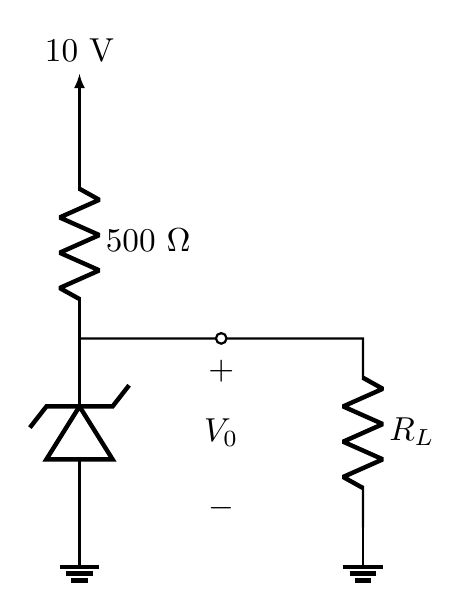
\begin{tikzpicture}[thick,scale=1.2, transform shape]
        
        % Top Voltage source arrow and label
        \draw[-latex] (0, 2) -- (0, 2.8) node[above] {$10\text{ V}$};
        
        % Top Resistor (500 Ohm)
        \draw (0, 2) to[R, l=$500\ \Omega$] (0, 0);
        
        % Zener Diode (drawn bottom-to-top so the cathode bar faces upwards)
        \draw (0, -2) node[ground]{} to[zzD] (0, 0);
        
        % Right branch to Load Resistor
        \draw (0, 0) -- (1.5, 0) node[ocirc]{} -- (3, 0) 
              to[R, l=$R_L$] (3, -2) node[ground]{};
        
        % Output Voltage Labels
        \node[below] at (1.5, -0.1) {$+$};
        \node at (1.5, -1) {$V_0$};
        \node at (1.5, -1.8) {$-$};
        
    \end{tikzpicture}
\end{center}
\mk{23} \yr{EEE 263 | L-2/T-1 | 2020--21}

\begin{tcolorbox}[enhanced,breakable,ansbox,colback=cA!4,colframe=cA,boxrule=0.8pt,arc=5pt,title={\textbf{Answer}},fonttitle=\bfseries\color{white},colbacktitle=cA]

\subsection*{1. Reference Circuit Diagram}
\begin{center}
    \begin{circuitikz}[thick, scale=1.0, transform shape, font=\sffamily]
        % Source Terminal
        \draw[<-] (0, 2) -- (0, 2.5) node[above] {$V_S = 10\text{ V}$};
        
        % Series Resistor
        \draw (0, 2) to[R, l=$500\ \Omega$, name=Rs] (0, 0);
        
        % Zener Diode
        \draw (0, -2) node[ground]{} to[zzD, l=$D_Z$, name=ZD] (0, 0);
        
        % Right branch to Load Resistor
        \draw (0, 0) -- (1.5, 0) node[ocirc]{} -- (3, 0) 
              to[R, l=$R_L$] (3, -2) node[ground]{};
        
        % Output Voltage Labels
        \node[below] at (1.5, -0.1) {$+$};
        \node at (1.5, -1) {$V_0$};
        \node[above] at (1.5, -1.9) {$-$};
        
        % Add current labels
        \draw[->, >=stealth, line width=0.8pt] (-0.3, 1.5) -- (-0.3, 0.5) node[midway, left] {$I_S$};
        \draw[->, >=stealth, line width=0.8pt] (0.3, -0.5) -- (0.3, -1.5) node[midway, right] {$I_Z$};
        \draw[->, >=stealth, line width=0.8pt] (2.7, -0.5) -- (2.7, -1.5) node[midway, left] {$I_L$};
    \end{circuitikz}
\end{center}

\vspace{0.5cm}

\subsection*{2. Theory \& Zener Model Evaluation}
To analyze this circuit accurately, we must replace the Zener diode with its piecewise linear equivalent model, which consists of a DC voltage source $V_{Z0}$ in series with an internal dynamic resistance $r_z$.

The governing equation for the Zener diode in the breakdown region is:
\begin{equation}
    V_Z = V_{Z0} + I_Z r_z
\end{equation}

Given the test conditions: $V_Z = 6.8\text{ V}$ at $I_Z = 5\text{ mA}$ and $r_z = 20\ \Omega$.
We can calculate the zero-current intercept voltage $V_{Z0}$:
\begin{align*}
    V_{Z0} &= V_Z - I_Z r_z \nonumber \\
    V_{Z0} &= 6.8 - (5 \times 10^{-3})(20) \nonumber \\
    V_{Z0} &= 6.8 - 0.1 \nonumber \\
    V_{Z0} &= 6.7\text{ V}
\end{align*}

\vspace{0.5cm}

\subsection*{3. Step-by-Step Mathematical Solution}

\subsubsection*{(i) Find $V_0$ at no-load conditions ($R_L = \infty$)}
Under no-load conditions, the load resistor is disconnected (open circuit), meaning the load current $I_L = 0$. Therefore, the entire supply current flows through the Zener diode ($I_S = I_Z$). 

Assuming the diode is operating in the breakdown region (which we will verify), we write the loop equation for the equivalent circuit:
\begin{align*}
    I_Z &= \frac{V_S - V_{Z0}}{R_S + r_z} \nonumber \\
    I_Z &= \frac{10 - 6.7}{500 + 20} \nonumber \\
    I_Z &= \frac{3.3}{520} \nonumber \\
    I_Z &\approx 6.346\text{ mA}
\end{align*}

\textit{Verification:} Since $I_Z \approx 6.346\text{ mA}$ is greater than $I_{ZK} (0.2\text{ mA})$, our assumption that the diode is in breakdown holds true.

Now, compute the output voltage $V_0$:
\begin{align*}
    V_0 &= V_{Z0} + I_Z r_z \nonumber \\
    V_0 &= 6.7 + (6.346 \times 10^{-3})(20) \nonumber \\
    V_0 &= 6.7 + 0.1269 \nonumber \\
    V_0 &= \mathbf{6.827\text{ V}}
\end{align*}

\subsubsection*{(ii) Minimum value of $R_L$ to maintain breakdown region}
To keep the Zener diode in the breakdown region, the current flowing through it must not drop below the knee current $I_{ZK} = 0.2\text{ mA}$. This boundary condition represents the maximum possible current drawn by the load before the Zener turns off.

At the threshold condition $I_Z = I_{ZK} = 0.2\text{ mA}$, the Zener voltage is:
\begin{align*}
    V_0 &= V_{Z0} + I_{ZK} r_z \nonumber \\
    V_0 &= 6.7 + (0.2 \times 10^{-3})(20) \nonumber \\
    V_0 &= 6.7 + 0.004 \nonumber \\
    V_0 &= 6.704\text{ V}
\end{align*}

Next, determine the total source current $I_S$ flowing through the $500\ \Omega$ series resistor:
\begin{align*}
    I_S &= \frac{V_S - V_0}{R_S} \nonumber \\
    I_S &= \frac{10 - 6.704}{500} \nonumber \\
    I_S &= \frac{3.296}{500} \nonumber \\
    I_S &= 6.592\text{ mA}
\end{align*}

Applying Kirchhoff's Current Law (KCL) at the top output node, we find the maximum allowable load current:
\begin{align*}
    I_{L(\text{max})} &= I_S - I_{ZK} \nonumber \\
    I_{L(\text{max})} &= 6.592\text{ mA} - 0.2\text{ mA} \nonumber \\
    I_{L(\text{max})} &= 6.392\text{ mA}
\end{align*}

Finally, calculate the corresponding minimum load resistance:
\begin{align*}
    R_{L(\text{min})} &= \frac{V_0}{I_{L(\text{max})}} \nonumber \\
    R_{L(\text{min})} &= \frac{6.704}{6.392 \times 10^{-3}} \nonumber \\
    R_{L(\text{min})} &\approx 1048.8\ \Omega \text{ or } \mathbf{1.049\text{ k}\Omega}
\end{align*}

\vspace{0.5cm}

\subsection*{4. Final Answer Summary}
\begin{center}
    \renewcommand{\arraystretch}{1.5}
    \begin{tabular}{@{}ll@{}}
        \toprule
        \textbf{Parameter} & \textbf{Calculated Value} \\
        \midrule
        Zener Zero-Current Intercept ($V_{Z0}$) & $6.7\text{ V}$ \\
        No-load Output Voltage ($V_0$) & $\mathbf{6.827\text{ V}}$ \\
        Minimum Load Resistance ($R_{L(\text{min})}$) & $\mathbf{1.049\text{ k}\Omega}$ \\
        \bottomrule
    \end{tabular}
\end{center}

\end{tcolorbox}

\item A voltage regulator circuit is to power a car radio at $V_L=9\,\text{V}$ from an automobile battery whose voltage may vary between 11 and 13.6\,V. The current in the radio will vary between 0 (off) and 100\,mA (full volume). Determine the value of the current-limiting resistor $R_i$ and the maximum power dissipated in the Zener diode.
\begin{center}
  
    \begin{circuitikz}[thick,scale=1.2, transform shape]
        
        % ==========================================
        % Voltage Source (Left Branch)
        % ==========================================
        % Drawn from bottom to top so the positive terminal (long line) is at the top
        \draw (0,3) to[battery] (0,0);
        
        % Manual labels for the battery to match the specific formatting in the image
        \node[left, align=center] at (-0.5, 1.5) {$V_{PS} =$\\$11-13.6\text{ V}$};
        \node[left] at (-0.2, 2.6) {$+$};
        \node[left] at (-0.2, 0.4) {$-$};
        
        % ==========================================
        % Series Resistor R1 (Top Branch)
        % ==========================================
        \draw (0,3) to[R, l=$R_i$, i=$I_I$] (4,3);
        
        % ==========================================
        % Zener Diode (Middle Branch)
        % ==========================================
        % Drawn from top to bottom. "invert" flips the diode so the cathode is facing up.
        % The current I_Z is drawn flowing downwards.
        \draw (4,3) to[zzD, invert, i=$I_Z$, *-*] (4,0);
        
        % Voltage labels for the Zener Diode
        \node[right] at (4.2, 2.5) {$+$};
        \node[right] at (4.2, 1.5) {$V_Z = 9\text{ V}$};
        \node[right] at (4.2, 0.5) {$-$};
        
        % ==========================================
        % Load - Radio (Right Branch)
        % ==========================================
        % Top wire with load current arrow
        \draw (4,3) to[short, i=$I_L$] (7.5,3);
        
        % Shaded Radio box
        \node[draw, fill=gray!30, minimum width=1.5cm, minimum height=1.2cm] (radio) at (7.5, 1.5) {Radio};
        
        % Connecting lines to the Radio box
        \draw (7.5,3) -- (radio.north);
        \draw (radio.south) -- (7.5,0);
        
        % ==========================================
        % Bottom Ground/Return Wire
        % ==========================================
        \draw (7.5,0) -- (0,0);

        
    \end{circuitikz}
\end{center}
\mk{18} \yr{EEE 263 | L-2/T-1 | 2017--18}

\begin{tcolorbox}[enhanced,breakable,ansbox,colback=cA!4,colframe=cA,boxrule=0.8pt,arc=5pt,title={\textbf{Answer}},fonttitle=\bfseries\color{white},colbacktitle=cA]

\subsection*{1. Reference Circuit Diagram}
\begin{center}
    \begin{circuitikz}[thick, scale=1.0, transform shape, font=\sffamily]
        
        % Voltage Source (Left Branch)
        \draw (0,3) to[battery1] (0,0);
        \node[left, align=center] at (-0.5, 1.5) {$V_{PS} =$ \\ $11-13.6\text{ V}$};
        \node[left] at (-0.2, 2.6) {$+$};
        \node[left] at (-0.2, 0.4) {$-$};
        
        % Series Resistor R_i (Top Branch)
        \draw (0,3) to[R, l=$R_i$, i=$I_I$] (4,3);
        
        % Zener Diode (Middle Branch)
        \draw (4,3) to[zzD, invert, i=$I_Z$, *-*] (4,0);
        \node[right] at (4.2, 2.5) {$+$};
        \node[right] at (4.2, 1.5) {$V_Z = 9\text{ V}$};
        \node[right] at (4.2, 0.5) {$-$};
        
        % Load - Radio (Right Branch)
        \draw (4,3) to[short, i=$I_L$] (7.5,3);
        \node[draw, fill=gray!20, minimum width=1.5cm, minimum height=1.2cm, rounded corners=2pt] (radio) at (7.5, 1.5) {\textbf{Radio}};
        \draw (7.5,3) -- (radio.north);
        \draw (radio.south) -- (7.5,0);
        
        % Bottom Ground/Return Wire
        \draw (7.5,0) -- (0,0);
        
    \end{circuitikz}
\end{center}

\vspace{0.3cm}

\subsection*{2. Principle of Operation \& Assumptions}
This circuit is a basic Zener voltage regulator operating under varying input voltage (line regulation) and varying load current (load regulation). To ensure the radio receives a stable $9\text{ V}$, the Zener diode must remain in the breakdown region under all operating conditions.

By Kirchhoff's Current Law (KCL) at the node above the Zener diode:
\begin{equation}
    I_I = I_Z + I_L \implies I_Z = I_I - I_L
\end{equation}
The input current $I_I$ is governed by Ohm's Law:
\begin{equation}
    I_I = \frac{V_{PS} - V_Z}{R_i}
\end{equation}

\textbf{Assumptions:}
\begin{itemize}
    \item The minimum Zener knee current $I_{ZK}$ is negligible ($I_{ZK} \approx 0\text{ mA}$) unless otherwise specified.
    \item The Zener voltage $V_Z$ remains perfectly constant at $9\text{ V}$ in the breakdown region (ideal Zener model).
\end{itemize}

\vspace{0.3cm}

\subsection*{3. Step-by-Step Mathematical Derivation}

\subsubsection*{Step 1: Determine the Current-Limiting Resistor ($R_i$)}
To maintain regulation, the Zener diode must not turn off. The worst-case condition for the Zener diode dropping out of regulation occurs when the input voltage is at its minimum and the load draws its maximum current.
\begin{align*}
    V_{PS(\text{min})} &= 11\text{ V} \\
    I_{L(\text{max})} &= 100\text{ mA} = 0.1\text{ A}
\end{align*}
Under this condition, the Zener current is at its minimum ($I_{Z(\text{min})} \approx 0\text{ A}$). 
\begin{align*}
    I_{I(\text{min})} &= I_{Z(\text{min})} + I_{L(\text{max})} \nonumber \\
    I_{I(\text{min})} &= 0 + 100\text{ mA} = 100\text{ mA}
\end{align*}
Now, substituting into the input current equation to solve for $R_i$:
\begin{align*}
    R_i &= \frac{V_{PS(\text{min})} - V_Z}{I_{I(\text{min})}} \nonumber \\
    R_i &= \frac{11\text{ V} - 9\text{ V}}{0.1\text{ A}} \nonumber \\
    R_i &= \frac{2\text{ V}}{0.1\text{ A}} \nonumber \\
    R_i &= \mathbf{20\ \Omega}
\end{align*}

\subsubsection*{Step 2: Determine Maximum Power Dissipated in the Zener Diode ($P_{Z(\text{max})}$)}
The worst-case condition for power dissipation in the Zener diode occurs when the input voltage is at its maximum and the load is disconnected (or turned off), meaning all input current is forced through the Zener diode.
\begin{align*}
    V_{PS(\text{max})} &= 13.6\text{ V} \\
    I_{L(\text{min})} &= 0\text{ A}
\end{align*}
First, calculate the maximum input current $I_{I(\text{max})}$ using the chosen $R_i$:
\begin{align*}
    I_{I(\text{max})} &= \frac{V_{PS(\text{max})} - V_Z}{R_i} \nonumber \\
    I_{I(\text{max})} &= \frac{13.6\text{ V} - 9\text{ V}}{20\ \Omega} \nonumber \\
    I_{I(\text{max})} &= \frac{4.6\text{ V}}{20\ \Omega} \nonumber \\
    I_{I(\text{max})} &= 0.23\text{ A} = 230\text{ mA}
\end{align*}
Since $I_{L(\text{min})} = 0$, the maximum Zener current is:
\begin{equation}
    I_{Z(\text{max})} = I_{I(\text{max})} - I_{L(\text{min})} = 230\text{ mA} - 0\text{ mA} = 230\text{ mA}
\end{equation}
Finally, calculate the maximum power dissipation:
\begin{align*}
    P_{Z(\text{max})} &= V_Z \times I_{Z(\text{max})} \nonumber \\
    P_{Z(\text{max})} &= 9\text{ V} \times 0.23\text{ A} \nonumber \\
    P_{Z(\text{max})} &= \mathbf{2.07\text{ W}}
\end{align*}

\vspace{0.3cm}

\subsection*{4. Final Answer Summary}
\begin{center}
    \renewcommand{\arraystretch}{1.5}
    \begin{tabular}{@{}ll@{}}
        \toprule
        \textbf{Parameter} & \textbf{Calculated Value} \\
        \midrule
        Current-Limiting Resistor ($R_i$) & $\mathbf{20\ \Omega}$ \\
        Maximum Zener Current ($I_{Z(\text{max})}$) & $230\text{ mA}$ \\
        Maximum Zener Power Dissipation ($P_{Z(\text{max})}$) & $\mathbf{2.07\text{ W}}$ \\
        \bottomrule
    \end{tabular}
\end{center}

\end{tcolorbox}

\item For the circuit shown in Figure , plot $v_0$ versus $v_{\text{i}}$ and $i_1$ versus $v_{\text{i}}$ over the range $-10 \le v_{\text{i}} \le +10\text{ V}$. Assume the diodes to be ideal.
 \begin{center}
\begin{circuitikz}[thick,scale=1.2, transform shape]
        
        % ==========================================
        % Input Stage
        % ==========================================
        % Input terminal and 10k Resistor with current label i_i
        \draw (0, 3) node[left] {\Large $v_i$} node[ocirc] {} 
              to[R, l=$10\text{ k}\Omega$, i_=$i_i$] (3, 3);
              
        % ==========================================
        % Zener Diode Section
        % ==========================================
        % Zener drawn right-to-left so it points left (cathode on the left)
        \draw (5, 3) to[zzD] (3, 3);
        
        % Manual placement for Zener labels (+, -, and Vz)
        \node at (3.3, 3.4) {\large $+$};
        \node at (4.7, 3.4) {\large $-$};
        \node at (4.0, 3.8) {$V_z=3\text{V}$};
        
        % ==========================================
        % Top Rail and Output
        % ==========================================
        % Junction dots
        \node[circ] at (5, 3) {};
        \node[circ] at (6.5, 3) {};
        
        % Wire extending to output terminal
        \draw (5, 3) -- (7.5, 3) node[ocirc] {} node[right] {\Large $v_o$};
        
        % ==========================================
        % Vertical Branches
        % ==========================================
        % Standard Diode pointing UP (cathode on top)
        \draw (5, 0) to[D] (5, 3);
        
        % 10k Output Resistor
        \draw (6.5, 3) to[R, l=$10\text{ k}\Omega$] (6.5, 0);
        
        % ==========================================
        % Ground Connection
        % ==========================================
        % Connect bottoms and attach ground
        \draw (5, 0) -- (6.5, 0);
        \node[ground] at (5.75, 0) {};
        
    \end{circuitikz}
\end{center}
\mk{13.67} \yr{EEE 263 | L-2/T-1 | 2016--17}

\begin{tcolorbox}[enhanced,breakable,ansbox,colback=cA!4,colframe=cA,boxrule=0.8pt,arc=5pt,title={\textbf{Answer}},fonttitle=\bfseries\color{white},colbacktitle=cA]

\subsection*{1. Reference Circuit Diagram}
\begin{center}
    \begin{circuitikz}[thick, scale=1.0, transform shape, font=\sffamily]
        
        % Input Stage
        \draw (0, 3) node[left] {$v_i$} node[ocirc] {} 
              to[R, l=$R_1 \; 10\text{ k}\Omega$, i>_=$i_1$] (3, 3);
              
        % Zener Diode Section
        \draw (5, 3) to[zzD, l=$D_Z$] (3, 3);
        \node at (3.3, 3.4) {$+$};
        \node at (4.7, 3.4) {$-$};
        \node at (4.0, 3.8) {$V_Z=3\text{ V}$};
        
        % Top Rail and Output
        \node[circ] at (5, 3) {};
        \node[circ] at (6.5, 3) {};
        \draw (5, 3) -- (7.5, 3) node[ocirc] {} node[right] {$v_o$};
        
        % Vertical Branches
        \draw (5, 0) to[D, l=$D_1$] (5, 3);
        \draw (6.5, 3) to[R, l=$R_L \; 10\text{ k}\Omega$] (6.5, 0);
        
        % Ground Connection
        \draw (5, 0) -- (6.5, 0);
        \node[ground] at (5.75, 0) {};
        
    \end{circuitikz}
\end{center}

\vspace{0.3cm}

\subsection*{2. Principle of Operation \& Assumptions}
The circuit evaluates an input voltage $v_i$ spanning from $-10\text{ V}$ to $+10\text{ V}$. 
\begin{itemize}
    \item \textbf{Ideal Diode Assumptions:} Both the Zener diode ($D_Z$) and the standard diode ($D_1$) are considered ideal. This means their forward voltage drops are $0\text{ V}$, their reverse leakage currents are $0\text{ A}$, and $D_Z$ exhibits a perfect vertical breakdown at exactly $V_Z = 3\text{ V}$.
    \item \textbf{Zener Orientation:} $D_Z$ has its cathode facing the input side. Therefore, it will be in Zener breakdown when the voltage at its cathode is $3\text{ V}$ more positive than its anode. It will be forward-biased when its anode is more positive than its cathode.
    \item \textbf{Standard Diode Orientation:} $D_1$ has its anode tied to ground. It will become forward-biased and act as a short circuit if $v_o$ attempts to drop below $0\text{ V}$.
\end{itemize}

\vspace{0.3cm}

\subsection*{3. Step-by-Step Mathematical Analysis}

The behavior of the circuit changes based on the input voltage $v_i$. We divide the input range into three distinct regions of operation.

\subsubsection*{Region I: $v_i < 0\text{ V}$}
When the input voltage is negative, the current $i_1$ attempts to flow from right to left (meaning $i_1$ will be negative). 
\begin{itemize}
    \item This polarity forward-biases the Zener diode ($D_Z$). Because it is ideal, it acts as a short circuit, meaning the voltage at the node between $R_1$ and $D_Z$ equals $v_o$.
    \item The negative voltage pulls $v_o$ below ground, which immediately forward-biases diode $D_1$. 
    \item As an ideal forward-biased diode, $D_1$ acts as a short to ground, clamping the output voltage: $v_o = 0\text{ V}$.
\end{itemize}
Since $v_o = 0\text{ V}$ and $D_Z$ is a short, the voltage at the right side of $R_1$ is $0\text{ V}$.
\begin{align*}
    i_1 &= \frac{v_i - 0}{10\text{ k}\Omega} = \frac{v_i}{10\text{ k}\Omega} \\
    v_o &= 0\text{ V}
\end{align*}
\textit{At $v_i = -10\text{ V}$, the current is $i_1 = -1\text{ mA}$.}

\subsubsection*{Region II: $0 \le v_i \le 3\text{ V}$}
When the input voltage is positive but has not yet exceeded the Zener breakdown threshold ($V_Z = 3\text{ V}$):
\begin{itemize}
    \item The output voltage $v_o$ will be $\ge 0$, ensuring $D_1$ remains reverse-biased (OFF).
    \item $v_i$ is not large enough to break down $D_Z$, so $D_Z$ remains in the reverse-blocking region and acts as an open circuit.
\end{itemize}
Since $D_Z$ acts as an open circuit, no current can flow through the input branch.
\begin{align*}
    i_1 &= 0\text{ mA} \\
    v_o &= 0\text{ V} \quad \text{(since no current flows through } R_L)
\end{align*}

\subsubsection*{Region III: $v_i > 3\text{ V}$}
When $v_i$ exceeds $3\text{ V}$, it provides sufficient potential to push $D_Z$ into the Zener breakdown region.
\begin{itemize}
    \item $D_Z$ acts as a constant $3\text{ V}$ voltage drop (opposing the input).
    \item $v_o$ is positive, so $D_1$ remains reverse-biased (OFF).
\end{itemize}
The circuit simplifies to a single series loop comprising $v_i$, $R_1$, the $3\text{ V}$ Zener drop, and $R_L$.
Applying Kirchhoff's Voltage Law (KVL):
\begin{align*}
    v_i - i_1 R_1 - V_Z - i_1 R_L &= 0 \nonumber \\
    i_1(10\text{ k}\Omega + 10\text{ k}\Omega) &= v_i - 3 \nonumber \\
    i_1 &= \frac{v_i - 3}{20\text{ k}\Omega}
\end{align*}
The output voltage is determined by the load resistor $R_L$:
\begin{align*}
    v_o &= i_1 \times R_L \nonumber \\
    v_o &= \left( \frac{v_i - 3}{20\text{ k}\Omega} \right) \times 10\text{ k}\Omega \nonumber \\
    v_o &= 0.5(v_i - 3)
\end{align*}
\textit{At $v_i = 10\text{ V}$, $i_1 = 7 / 20\text{ k}\Omega = 0.35\text{ mA}$ and $v_o = 0.5(10 - 3) = 3.5\text{ V}$.}

\vspace{0.3cm}

\subsection*{4. Transfer Characteristics}

\begin{center}
    \begin{minipage}{0.48\textwidth}
        \centering
        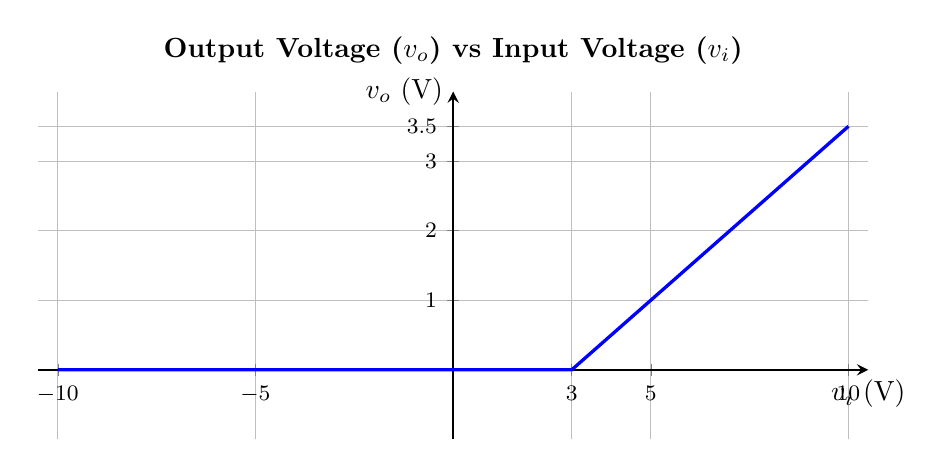
\begin{tikzpicture}
            \begin{axis}[
                width=1.0\textwidth, height=6cm,
                title={\textbf{Output Voltage ($v_o$) vs Input Voltage ($v_i$)}},
                xlabel={$v_i$ (V)}, ylabel={$v_o$ (V)},
                xmin=-10.5, xmax=10.5, ymin=-1, ymax=4,
                grid=major, axis lines=middle,
                xtick={-10,-5,0,3,5,10}, ytick={0,1,2,3,3.5},
                xlabel style={anchor=north}, ylabel style={anchor=east},
                tick label style={font=\footnotesize}
            ]
            \addplot[blue, very thick] coordinates {(-10,0) (3,0) (10,3.5)};
            \end{axis}
        \end{tikzpicture}
    \end{minipage}\hfill
    \begin{minipage}{0.48\textwidth}
        \centering
        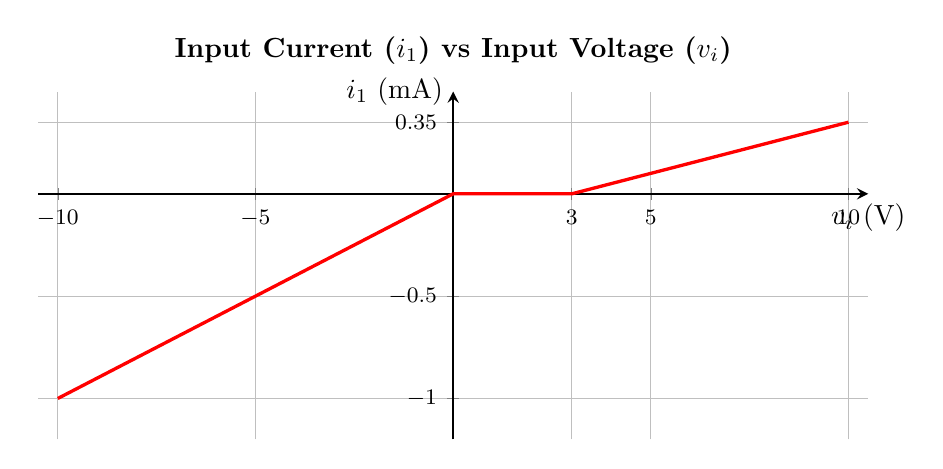
\begin{tikzpicture}
            \begin{axis}[
                width=1.0\textwidth, height=6cm,
                title={\textbf{Input Current ($i_1$) vs Input Voltage ($v_i$)}},
                xlabel={$v_i$ (V)}, ylabel={$i_1$ (mA)},
                xmin=-10.5, xmax=10.5, ymin=-1.2, ymax=0.5,
                grid=major, axis lines=middle,
                xtick={-10,-5,0,3,5,10}, ytick={-1,-0.5,0,0.35},
                xlabel style={anchor=north}, ylabel style={anchor=east},
                tick label style={font=\footnotesize}
            ]
            \addplot[red, very thick] coordinates {(-10,-1) (0,0) (3,0) (10,0.35)};
            \end{axis}
        \end{tikzpicture}
    \end{minipage}
\end{center}

\vspace{0.3cm}

\subsection*{5. Summary of Equations}
The piecewise functions governing the output voltage and input current over the entire range are summarized below:

\begin{equation}
    v_o = 
    \begin{cases} 
        0\text{ V} & \text{for } -10\text{ V} \le v_i \le 3\text{ V} \\
        0.5(v_i - 3)\text{ V} & \text{for } 3\text{ V} < v_i \le 10\text{ V}
    \end{cases}
\end{equation}

\vspace{0.2cm}

\begin{equation}
    i_1 = 
    \begin{cases} 
        \frac{v_i}{10\text{ k}\Omega} & \text{for } -10\text{ V} \le v_i < 0\text{ V} \\[6pt]
        0\text{ mA} & \text{for } 0\text{ V} \le v_i \le 3\text{ V} \\[6pt]
        \frac{v_i - 3}{20\text{ k}\Omega} & \text{for } 3\text{ V} < v_i \le 10\text{ V}
    \end{cases}
\end{equation}

\end{tcolorbox}

\item For the circuit shown, find $V_a$ and $I_z$. Now if $R_1$ and $R_2$ are swapped, what will be the value of $V_a$ and $I_z$?
\begin{center}
  
    \begin{circuitikz}[thick,scale=1.2, transform shape]
        
        % ১. DC Voltage Source
        % battery1 ব্যবহার করলে ডিফল্টভাবে উপরের দিকে পজিটিভ (বড় দাগ) থাকে
        \draw (0,2.5) to[battery1] (0,0);
        \node at (-0.6, 2.2) {$+$};
        \node at (-0.7, 1.25) {$10\mathrm{V}$};
        \node at (-0.6, 0.3) {$-$};
        
        % ২. R1 Resistor and Top Wire
        \draw (0,2.5) to[R, l={$R_1=2\mathrm{K}\Omega$}] (3,2.5) coordinate (top_mid);
        \draw (0,0) -- (3,0) coordinate (bot_mid);
        
        % ৩. Zener Diode Branch
        % জেনার ডায়োডটি নিচ থেকে উপরে আঁকা হয়েছে যেন ক্যাথোড (দাগ দেওয়া অংশ) উপরে থাকে
        \draw (bot_mid) to[zzD] (top_mid); 
        
        % Zener Labels (Current and Voltage)
        % Iz কারেন্টের জন্য আলাদা একটি তীর (arrow) আঁকা হয়েছে
        \draw[->, >=stealth] (2.4, 1.8) -- (2.4, 0.7) node[midway, left] {$I_Z$};
        \node[right, align=left] at (3.4, 1.25) {$5\mathrm{V}$\\zener};
        
        % ৪. R2 Resistor Branch
        \draw (top_mid) -- (5,2.5) coordinate (top_right);
        \draw (bot_mid) -- (5,0) coordinate (bot_right);
        \draw (top_right) to[R, l={$R_2=3\mathrm{K}\Omega$} , a=$V_a$] (bot_right);
        
        % ৫. Output Terminals (Vo)
        \draw (top_right) to[short, -o] (6,2.5) node[above] {$+$};
        \draw (bot_right) to[short, -o] (6,0) node[below] {$-$};

        
    \end{circuitikz}
\end{center}

\mk{15} \yr{EEE 263 | L-2/T-1 | 2015--16}

\begin{tcolorbox}[enhanced,breakable,ansbox,colback=cA!4,colframe=cA,boxrule=0.8pt,arc=5pt,title={\textbf{Answer}},fonttitle=\bfseries\color{white},colbacktitle=cA]

\subsubsection*{1. Initial Circuit Configuration Analysis}

\textbf{Circuit Diagram:}
\begin{center}
    \begin{circuitikz}[american, thick, scale=1.0, transform shape]
        % DC Voltage Source
        \draw (0,3) to[battery1, l_=$10\,\text{V}$] (0,0);
        
        % R1 Resistor and Top Wire
        \draw (0,3) to[R, l={$R_1=2\,\text{k}\Omega$}, i_=$I_{R1}$] (3,3) coordinate (top_mid);
        \draw (0,0) -- (3,0) coordinate (bot_mid);
        
        % Zener Diode Branch
        \draw (bot_mid) to[zzD, l_=$5\,\text{V}$, i<_=$I_Z$] (top_mid); 
        
        % R2 Resistor Branch
        \draw (top_mid) -- (6,3) coordinate (top_right);
        \draw (bot_mid) -- (6,0) coordinate (bot_right);
        \draw (top_right) to[R, l={$R_2=3\,\text{k}\Omega$}, i=$I_{R2}$, a=$V_a$] (bot_right);
        
        % Output Terminals (Va)
        \draw (top_right) to[short, -o] (7,3) node[above] {$+$};
        \draw (bot_right) to[short, -o] (7,0) node[below] {$-$};        
        % Ground
        \draw (bot_mid) node[ground]{};
    \end{circuitikz}
\end{center}

\textbf{Step 1.1: State and Verify Assumption} \\
To determine the operating state of the Zener diode, we first assume it is \textbf{OFF} (acting as an open circuit). We then calculate the Thevenin voltage ($V_{Th}$) across the open Zener terminals, which is simply the voltage across $R_2$ determined by the voltage divider formed by $R_1$ and $R_2$:
\begin{align*}
    V_{Th} &= V_{in} \left( \frac{R_2}{R_1 + R_2} \right) \notag \\
    &= 10\,\text{V} \left( \frac{3\,\text{k}\Omega}{2\,\text{k}\Omega + 3\,\text{k}\Omega} \right) \notag \\
    &= 10 \left( \frac{3}{5} \right) = \mathbf{6\,\text{V}}
\end{align*}

Since the open-circuit voltage ($V_{Th} = 6\,\text{V}$) is greater than the Zener breakdown voltage ($V_Z = 5\,\text{V}$), our initial assumption is incorrect. \textbf{The Zener diode is ON and operating in the breakdown region.}

\textbf{Step 1.2: Calculate Output Voltage ($V_a$) and Zener Current ($I_Z$)} \\
Because the Zener is in breakdown and in parallel with the load $R_2$, it firmly clamps the output voltage to its nominal value:
\begin{equation}
    V_a = V_Z = \mathbf{5\,\text{V}}
\end{equation}

Next, we apply Kirchhoff's Current Law (KCL) at the upper node:
\begin{equation}
    I_{R1} = I_Z + I_{R2} \implies I_Z = I_{R1} - I_{R2}
\end{equation}

Calculating the individual branch currents:
\begin{align*}
    I_{R1} &= \frac{V_{in} - V_a}{R_1} = \frac{10\,\text{V} - 5\,\text{V}}{2\,\text{k}\Omega} = \frac{5}{2}\,\text{mA} = 2.5\,\text{mA} \\
    I_{R2} &= \frac{V_a}{R_2} = \frac{5\,\text{V}}{3\,\text{k}\Omega} \approx 1.667\,\text{mA}
\end{align*}

Substituting these into the KCL equation:
\begin{equation}
    I_Z = 2.5\,\text{mA} - 1.667\,\text{mA} = \mathbf{0.833\,\text{mA}}
\end{equation}

 
\vspace{1em}

\subsubsection*{2. Swapped Resistors Configuration Analysis}

\textbf{Circuit Diagram:} (With $R_1$ and $R_2$ swapped)
\begin{center}
    \begin{circuitikz}[american, thick, scale=1.0, transform shape]
        % DC Voltage Source
        \draw (0,3) to[battery1, l_=$10\,\text{V}$] (0,0);
        
        % Swapped R1 Resistor and Top Wire
        \draw (0,3) to[R, l={$R_1'=3\,\text{k}\Omega$}] (3,3) coordinate (top_mid);
        \draw (0,0) -- (3,0) coordinate (bot_mid);
        
        % Zener Diode Branch
        \draw (bot_mid) to[zzD, l_=$5\,\text{V}$, i<_=$I_Z$] (top_mid); 
        
        % Swapped R2 Resistor Branch
        \draw (top_mid) -- (6,3) coordinate (top_right);
        \draw (bot_mid) -- (6,0) coordinate (bot_right);
        \draw (top_right) to[R, l={$R_2'=2\,\text{k}\Omega$}, a=$V_a$] (bot_right);
        
        % Output Terminals (Va)
        \draw (top_right) to[short, -o] (7,3) node[above] {$+$};
        \draw (bot_right) to[short, -o] (7,0) node[below] {$-$};
        % Ground
        \draw (bot_mid) node[ground]{};
    \end{circuitikz}
\end{center}

\textbf{Step 2.1: State and Verify Assumption} \\
Once again, assume the Zener diode is \textbf{OFF} (open circuit). We calculate the new Thevenin voltage ($V_{Th}'$) across the Zener terminals with the swapped resistor values ($R_1' = 3\,\text{k}\Omega$, $R_2' = 2\,\text{k}\Omega$):
\begin{align*}
    V_{Th}' &= V_{in} \left( \frac{R_2'}{R_1' + R_2'} \right) \notag \\
    &= 10\,\text{V} \left( \frac{2\,\text{k}\Omega}{3\,\text{k}\Omega + 2\,\text{k}\Omega} \right) \notag \\
    &= 10 \left( \frac{2}{5} \right) = \mathbf{4\,\text{V}}
\end{align*}

Since the available open-circuit voltage ($V_{Th}' = 4\,\text{V}$) is strictly less than the Zener breakdown voltage ($V_Z = 5\,\text{V}$), our assumption holds true. \textbf{The Zener diode remains OFF} and does not enter the breakdown region. 

\textbf{Step 2.2: Calculate Output Voltage ($V_a$) and Zener Current ($I_Z$)} \\
Because the Zener is OFF, it draws no current and acts as an open circuit. The circuit behaves entirely as a simple linear voltage divider.
\begin{align*}
    V_a &= V_{Th}' = \mathbf{4\,\text{V}} \\
    I_Z &= \mathbf{0\,\text{mA}}
\end{align*}

 
\vspace{1em}

\subsubsection*{3. Final Answer Summary}

\begin{center}
\renewcommand{\arraystretch}{1.5}
\begin{tabular}{@{}llcc@{}}
\toprule
\textbf{Condition} & \textbf{Zener State} & $\mathbf{V_a}$ \textbf{(Output Voltage)} & $\mathbf{I_Z}$ \textbf{(Zener Current)} \\ \midrule
Initial ($R_1 = 2\,\text{k}\Omega$, $R_2 = 3\,\text{k}\Omega$) & \textbf{ON} (Breakdown) & $5.00\,\text{V}$ & $0.833\,\text{mA}$ \\ 
Swapped ($R_1 = 3\,\text{k}\Omega$, $R_2 = 2\,\text{k}\Omega$) & \textbf{OFF} (Open) & $4.00\,\text{V}$ & $0\,\text{mA}$ \\ 
\bottomrule
\end{tabular}
\end{center}

\end{tcolorbox}

\item Calculate the regulated load voltage $V_L$ and the current $I_Z$ flowing through the zener diode in the voltage regulator circuit shown.
\begin{center}
      \begin{circuitikz}[thick,scale=1.2, transform shape]
        
        % ===================================================
        % Zener Diode & BJT Regulator Circuit
        % ===================================================
        
        % 1. Input 30V DC Source
        \draw (0,3) to[battery1, l={$30\mathrm{V}$}] (0,0) node[ground]{};
        
        % 2. 1.5k Ohm Resistor on top wire
        \draw (0,3) to[R, l={$1.5\mathrm{k}\Omega$}] (3,3);
        
        % 3. Zener Diode branch
        % Drawn from bottom to top so the cathode (bar) is at the top
        \draw (3,1.5) to[zzD, l_={$V_Z=9.3\mathrm{V}$}] (3,3);
        
        % Iz Current Arrow (drawn manually for exact placement like the image)
        \draw[->, >=stealth] (2.2, 2.7) -- (2.2, 1.8) node[midway, left] {$I_Z$};
        
        % 4. NPN BJT (Positioned cleanly at coordinates 5, 1.5)
        \node[npn] (Q1) at (5, 1.5) {};
        \node at (6.1, 1.5) {$\beta_{DC}=100$};
        
        % 5. Connections to BJT using its built-in anchors (Base, Collector, Emitter)
        % Base connection from Zener branch junction to Q1.B
        \draw (3,1.5) node[circ]{} -- (Q1.B);
        
        % Collector connection going UP from Q1.C to the top wire
        \draw (Q1.C) -- (5,3);
        
        % Emitter connection going DOWN from Q1.E to ground
        \draw (Q1.E) -- (5,0) node[ground]{};
        
        % 6. Top wire connecting Zener, BJT Collector, and Output
        \draw (3,3) node[circ]{} -- (5,3) node[circ]{} -- (7.5,3);
        
        % 7. Output terminal and Load Resistor (RL)
        \draw (7.5,3) node[ocirc]{} to[R, l={$R_L=1\mathrm{k}\Omega$}] (7.5,0) node[ground]{};
        
        % 8. VL Voltage Label (+, arrow, -) placed left of the load resistor
        \node at (9.7, 2.7) {$+$};
        \draw[->, >=stealth] (9.7, 2.4) -- (9.7, 0.6) node[midway, right] {$V_L$};
        \node at (9.7, 0.3) {$-$};
        
    \end{circuitikz}
\end{center}
\mk{16} \yr{EEE 263 | L-2/T-1 | 2014--15}

\begin{tcolorbox}[enhanced,breakable,ansbox,colback=cA!4,colframe=cA,boxrule=0.8pt,arc=5pt,title={\textbf{Answer}},fonttitle=\bfseries\color{white},colbacktitle=cA]

\subsection*{1. Circuit Diagram and Operating Principle}

The circuit presented is a \textbf{BJT-amplified shunt voltage regulator}. It combines a Zener diode for voltage reference with an NPN BJT to significantly increase the current-handling (shunting) capability of the regulator. The Zener diode determines the base voltage of the transistor relative to the output, while the BJT absorbs the bulk of the excess current from the unregulated supply, providing a stable load voltage $V_L$.

\begin{center}
    \begin{circuitikz}[thick, scale=1.0, transform shape]
        % 1. Input 30V DC Source
        \draw (0,3) to[battery1, l={$V_{in}=30\,\mathrm{V}$}] (0,0) node[ground]{};
        
        % 2. 1.5k Ohm Resistor on top wire
        \draw (0,3) to[R, l={$R_S=1.5\,\mathrm{k}\Omega$}] (3,3);
        
        % 3. Zener Diode branch
        \draw (3,1.5) to[zzD, l_={$V_Z=9.3\,\mathrm{V}$}] (3,3);
        
        % Iz Current Arrow
        \draw[->, >=stealth] (2.2, 2.7) -- (2.2, 1.8) node[midway, left] {$I_Z$};
        
        % 4. NPN BJT
        \node[npn] (Q1) at (5, 1.5) {};
        \node[right] at (5.5, 1.5) {$\beta_{DC}=100$};
        
        % 5. Connections to BJT
        \draw (3,1.5) node[circ]{} -- (Q1.B);
        \draw (Q1.C) -- (5,3);
        \draw (Q1.E) -- (5,0) node[ground]{};
        
        % 6. Top wire connecting Zener, BJT Collector, and Output
        \draw (3,3) node[circ]{} -- (5,3) node[circ]{} -- (7.5,3);
        
        % 7. Output terminal and Load Resistor (RL)
        \draw (7.5,3) node[circ]{} to[R, l={$R_L=1\,\mathrm{k}\Omega$}] (7.5,0) node[ground]{};
        
        % 8. VL Voltage Label
        \draw (7.5,3) -- (8.5,3) node[ocirc]{};
        \draw (7.5,0) -- (8.5,0) node[ocirc]{};
        \node at (8.5, 3.4) {$+$};
        \draw[->, >=stealth] (8.5, 2.8) -- (8.5, 0.2) node[midway, right] {$V_L$};
        \node at (8.5, -0.4) {$-$};
    \end{circuitikz}
\end{center}

\subsection*{2. Operating State Assumptions}
To perform the DC analysis, we make the following standard assumptions for an active voltage regulator:
\begin{itemize}
    \item \textbf{Zener Diode:} Operates in the \textbf{breakdown region}, maintaining a constant reverse voltage $V_Z = 9.3\,\mathrm{V}$.
    \item \textbf{NPN BJT:} Operates in the \textbf{forward-active region} with a base-emitter ON voltage $V_{BE(on)} \approx 0.7\,\mathrm{V}$.
\end{itemize}

\subsection*{3. Mathematical Derivation and Solution}

\textbf{Step 3a: Calculate Regulated Load Voltage ($V_L$)}\\
By applying Kirchhoff's Voltage Law (KVL) from the output node, down through the Zener diode and the BJT's base-emitter junction to ground, we find:
\begin{equation}
    V_L - V_Z - V_{BE(on)} = 0
\end{equation}
Rearranging to solve for the load voltage $V_L$:
\begin{align*}
    V_L &= V_Z + V_{BE(on)} \\
    &= 9.3\,\mathrm{V} + 0.7\,\mathrm{V} \\
    &= 10.0\,\mathrm{V}
\end{align*}

\textbf{Step 3b: Current Analysis (Source and Load Currents)}\\
The total current supplied by the unregulated source ($I_S$) flows through the series resistor $R_S$:
\begin{align*}
    I_S &= \frac{V_{in} - V_L}{R_S} \\
    &= \frac{30\,\mathrm{V} - 10\,\mathrm{V}}{1.5\,\mathrm{k}\Omega} = \frac{20\,\mathrm{V}}{1.5\,\mathrm{k}\Omega} = 13.333\,\mathrm{mA}
\end{align*}
The current drawn by the load resistor ($I_L$) is:
\begin{align*}
    I_L &= \frac{V_L}{R_L} \\
    &= \frac{10\,\mathrm{V}}{1\,\mathrm{k}\Omega} = 10.0\,\mathrm{mA}
\end{align*}

\textbf{Step 3c: Calculate Zener Current ($I_Z$)}\\
By applying Kirchhoff's Current Law (KCL) at the top regulated node, the total current entering the parallel shunt elements (Zener and BJT collector) is defined as $I_{shunt}$:
\begin{equation}
    I_{shunt} = I_S - I_L = 13.333\,\mathrm{mA} - 10.0\,\mathrm{mA} = 3.333\,\mathrm{mA}
\end{equation}
This shunt current splits between the Zener diode and the BJT collector:
\begin{equation}
    I_{shunt} = I_Z + I_C
\end{equation}
From the circuit topology, the Zener current $I_Z$ flows directly into the base of the BJT. Therefore:
\begin{equation}
    I_B = I_Z
\end{equation}
Assuming forward-active operation, the collector current is given by $I_C = \beta_{DC} I_B = \beta_{DC} I_Z$. Substituting this into the shunt current equation gives:
\begin{align*}
    I_{shunt} &= I_Z + \beta_{DC} I_Z \\
    I_{shunt} &= (\beta_{DC} + 1) I_Z
\end{align*}
Now, we can solve for $I_Z$:
\begin{align*}
    I_Z &= \frac{I_{shunt}}{\beta_{DC} + 1} \\
    &= \frac{3.333\,\mathrm{mA}}{100 + 1} \\
    &= \frac{3.333\,\mathrm{mA}}{101} \\
    &\approx 0.033\,\mathrm{mA} \quad (\text{or } 33.0\,\mu\mathrm{A})
\end{align*}

\subsection*{4. Verification of Operating Regions}
\begin{itemize}
    \item \textbf{Zener Verification:} Since the calculated Zener current is $I_Z = 33\,\mu\mathrm{A} > 0$, the Zener diode is actively conducting and correctly operating in the breakdown region.
    \item \textbf{BJT Verification:} The collector-emitter voltage is $V_{CE} = V_L = 10\,\mathrm{V}$. Because $V_{CE} = 10\,\mathrm{V} \gg V_{CE(sat)}$ (which is typically around $0.2\,\mathrm{V}$), the assumption that the BJT is in the forward-active region is strongly verified.
\end{itemize}

\subsection*{5. Final Answer Summary}
\begin{center}
    \renewcommand{\arraystretch}{1.5}
    \begin{tabular}{@{}ll@{}}
        \toprule
        \textbf{Calculated Parameter} & \textbf{Final Value} \\
        \midrule
        Regulated Load Voltage ($V_L$) & $\mathbf{10.0\,\mathrm{V}}$ \\
        Current through Zener Diode ($I_Z$) & $\mathbf{33.0\,\mu\mathrm{A}}$ \quad ($0.033\,\mathrm{mA}$) \\
        \bottomrule
    \end{tabular}
\end{center}

\end{tcolorbox}

\end{enumerate}



%%──────────────────────────────────────────────────────────────────────
\subtopic{cA}{Battery Charger Circuit}
\label{sub:s1-battery}

\begin{enumerate}
    
\item The circuit shown is for charging a 5\,V battery with $V_s = 10\sin(100\pi t)$. Find:
\begin{enumerate}
  \item Duty cycle (fraction of each cycle during which the diode conducts).
  \item Draw the diode current waveform indicating peak value.
  \item Maximum reverse bias voltage that appears across the diode.
\end{enumerate}
\begin{center}
      \begin{circuitikz}[thick,scale=1.2, transform shape]
        
        % 1. AC Source (Left Branch)
        \draw (0,0) to[sV] (0,2.5);
        \node[left] at (-0.4, 1.25) {$v_s$};
        \node at (-0.3, 2.1) {$+$};
        \node at (-0.3, 0.4) {$-$};
        
        % 2. Top Branch (Resistor & Diode)
        % i=$i_D$ দিয়ে ডায়োডের সাথে কারেন্টের দিক দেখানো হয়েছে
        \draw (0,2.5) to[R, l=$100\Omega$] (2.5, 2.5) 
              to[D, i=$i_D$] (5, 2.5);
        
        % 3. DC Source / Battery (Right Branch)
        \draw (5, 2.5) to[battery1] (5, 0);
        \node[right] at (5.3, 1.25) {$5\mathrm{V}$};
        \node at (4.6, 2.1) {$+$};
        \node at (4.6, 0.4) {$-$};
        
        % 4. Bottom Branch (Wire)
        \draw (0,0) -- (5,0);
        
    \end{circuitikz}
\end{center}
\mk{15} \yr{EEE 263 | L-2/T-1 | 2015--16}

\begin{tcolorbox}[enhanced,breakable,ansbox,colback=cA!4,colframe=cA,boxrule=0.8pt,arc=5pt,title={\textbf{Answer}},fonttitle=\bfseries\color{white},colbacktitle=cA]

\subsection*{1. Circuit Operation and Principle}
The given circuit consists of an AC voltage source $v_s(t) = 10\sin(100\pi t)$ in series with a resistor $R = 100\,\Omega$, an ideal diode $D$, and a DC battery $V_B = 5\text{ V}$. 

\begin{itemize}
    \item \textbf{Diode ON State (Conduction Region):} The ideal diode conducts when it is forward-biased. This occurs when the anode voltage exceeds the cathode voltage. Since the cathode is connected to the positive terminal of the $5\text{ V}$ battery, the diode turns ON when:
    \[ v_s(t) > 5\text{ V} \]
    During this period, the circuit is closed, and current $i_D(t)$ flows into the battery to charge it.
    \item \textbf{Diode OFF State (Non-Conduction Region):} When $v_s(t) < 5\text{ V}$, the diode is reverse-biased and acts as an open circuit. Consequently, the diode current is:
    \[ i_D(t) = 0\text{ A} \]
\end{itemize}

---

\subsection*{2. Step-by-Step Mathematical Derivation and Solution}

\subsubsection*{(a) Duty Cycle Calculation}
The duty cycle is defined as the fraction of each cycle during which the diode conducts. 

Let the total period of the input AC signal be $T$. The angular frequency is given as $\omega = 100\pi\text{ rad/s}$, so the time period $T$ is:
\[ T = \frac{2\pi}{\omega} = \frac{2\pi}{100\pi} = 0.02\text{ s} = 20\text{ ms} \]

The diode starts conducting at an angle $\theta_1$ when $v_s(t)$ rises to $5\text{ V}$:
\[ 10\sin(\theta_1) = 5 \implies \sin(\theta_1) = \frac{5}{10} = 0.5 \]
\[ \theta_1 = \arcsin(0.5) = \frac{\pi}{6}\text{ rad} \quad (30^\circ) \]

The diode stops conducting during the positive half-cycle when $v_s(t)$ falls below $5\text{ V}$ at angle $\theta_2$:
\[ \theta_2 = \pi - \theta_1 = \pi - \frac{\pi}{6} = \frac{5\pi}{6}\text{ rad} \quad (150^\circ) \]

The total conduction angle ($\theta_c$) within one full cycle ($2\pi$ rad) is:
\[ \theta_c = \theta_2 - \theta_1 = \frac{5\pi}{6} - \frac{\pi}{6} = \frac{4\pi}{6} = \frac{2\pi}{3}\text{ rad} \quad (120^\circ) \]

The duty cycle ($D$) is the ratio of the conduction angle to the total angle of one cycle ($2\pi$):
\[ D = \frac{\theta_c}{2\pi} = \frac{\frac{2\pi}{3}}{2\pi} = \frac{1}{3} \approx 33.33\% \]

\subsubsection*{(b) Diode Current Waveform and Peak Value}
When the diode is ON ($v_s > 5\text{ V}$), the current $i_D(t)$ is found by applying Kirchhoff's Voltage Law (KVL) around the loop:
\[ v_s(t) - i_D(t)R - V_B = 0 \implies i_D(t) = \frac{v_s(t) - 5}{100} \]

The peak diode current ($I_{D,\text{peak}}$) occurs when $v_s(t)$ reaches its maximum value of $10\text{ V}$ (at $\omega t = \pi/2$):
\[ I_{D,\text{peak}} = \frac{10 - 5}{100} = \frac{5}{100} = 0.05\text{ A} = 50\text{ mA} \]

The current expression during conduction ($\frac{\pi}{6} \le \omega t \le \frac{5\pi}{6}$) is:
\[ i_D(t) = \frac{10\sin(100\pi t) - 5}{100} = 0.1\sin(100\pi t) - 0.05 \quad \text{[A]} \]

\subsubsection*{(c) Maximum Reverse Bias Voltage (Peak Inverse Voltage - PIV)}
When the diode is reverse-biased ($v_s < 5\text{ V}$), it acts as an open circuit ($i_D = 0$). The voltage across the diode $v_D(t)$ (anode to cathode) is:
\[ v_D(t) = v_s(t) - V_B = v_s(t) - 5 \]

The maximum reverse bias voltage occurs when $v_s(t)$ reaches its most negative peak value, which is $-10\text{ V}$:
\[ v_{D,\text{min}} = -10 - 5 = -15\text{ V} \]

Thus, the maximum reverse bias voltage magnitude (Peak Inverse Voltage) is:
\[ \text{PIV} = |v_{D,\text{min}}| = 15\text{ V} \]

---

\subsection*{3. Circuit Diagrams and Waveforms}

\subsubsection*{Circuit Schematic}
\begin{center}
\begin{circuitikz}[thick, scale=1.0]
    % AC Source
    \draw (0,0) to[sV, l=$v_s$, v>=$~$] (0,3);
    
    % Resistor and Diode
    \draw (0,3) to[R, l=$100\,\Omega$] (2.5,3)
          to[D, i=$i_D$] (5,3);
          
    % Battery / DC Source
    \draw (5,3) to[battery1, l=$5\text{ V}$, v>=$~$] (5,0);
    
    % Bottom connection
    \draw (0,0) -- (5,0);
\end{circuitikz}
\end{center}

\subsubsection*{Diode Current Waveform}
\begin{center}
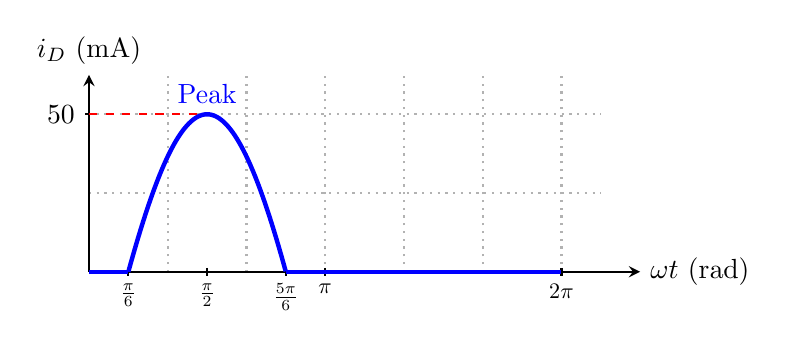
\begin{tikzpicture}[scale=1.0, >=stealth]
    % Grid lines
    \draw[dotted, gray!60] (0,0) grid (6.5,2.5);
    
    % Axes
    \draw[->, thick] (0,0) -- (7,0) node[right] {$\omega t$ (rad)};
    \draw[->, thick] (0,0) -- (0,2.5) node[above] {$i_D$ (mA)};
    
    % Important ticks on horizontal axis
    \draw (0.5,0.05) -- (0.5,-0.05) node[below, scale=0.8] {$\frac{\pi}{6}$};
    \draw (2.5,0.05) -- (2.5,-0.05) node[below, scale=0.8] {$\frac{5\pi}{6}$};
    \draw (3.0,0.05) -- (3.0,-0.05) node[below, scale=0.8] {$\pi$};
    \draw (6.0,0.05) -- (6.0,-0.05) node[below, scale=0.8] {$2\pi$};
    \draw (1.5,0.05) -- (1.5,-0.05) node[below, scale=0.8] {$\frac{\pi}{2}$};
    
    % Peak current indicator
    \draw[dashed, red] (0,2) -- (1.5,2);
    \draw (0,2) -- (-0.05,2) node[left] {$50$};
    
    % Waveform plot
    \draw[ultra thick, blue] (0,0) -- (0.5,0);
    \draw[ultra thick, blue, domain=0.5:2.5, samples=100] plot (\x, {4*sin((\x*180/3)) - 2});
    \draw[ultra thick, blue] (2.5,0) -- (6.0,0);
    
    % Labels
    \node[blue, above] at (1.5,2) {Peak};
\end{tikzpicture}
\end{center}

---

\subsection*{4. Final Answers Summary}

\begin{center}
\begin{tabular}{ccc}
    \toprule
    \textbf{Parameter} & \textbf{Symbol / Expression} & \textbf{Value} \\
    \midrule
    Conduction Angle & $\theta_c = \theta_2 - \theta_1$ & $\frac{2\pi}{3}\text{ rad } (120^\circ)$ \\
    \textbf{Duty Cycle} & $D = \frac{\theta_c}{2\pi}$ & $\mathbf{\frac{1}{3} \approx 33.33\%}$ \\
    \textbf{Peak Diode Current} & $I_{D,\text{peak}} = \frac{V_m - V_B}{R}$ & $\mathbf{50\text{ mA}}$ \\
    \textbf{Maximum Reverse Voltage} & $\text{PIV} = V_m + V_B$ & $\mathbf{15\text{ V}}$ \\
    \bottomrule
\end{tabular}
\end{center}

\end{tcolorbox}

\item A circuit for charging a 10\,V battery is shown in the figure. If $V_s$ is a sinusoid with 20\,V peak amplitude, find the fraction of each cycle during which the diode conducts. Assume the diode is ideal. Also find the peak value of the diode current and the maximum reverse bias voltage that appears across the diode.

\begin{center}
\begin{circuitikz}[thick,american, thick, scale=1.2, transform shape]
  
  % Left branch (Voltage Source)
  \draw (0,3) to[V, l=$v_s$] (0,0);
  
  % Top branch (Resistor and Diode)
  \draw (0,3) to[R, l_=$100\,\Omega$] (3,3)
        to[D] (6,3);
  
  % Right branch (Battery)
  \draw (6,3) to[battery1] (6,0);
  
  % Manual labels for the 10V battery
  \node at (6.6, 2.5) {$+$};
  \node at (6.6, 1.5) {$10\text{V}$};
  \node at (6.6, 0.5) {$-$};
  
  % Bottom return wire
  \draw (0,0) -- (6,0);
  
\end{circuitikz}
\end{center}

\mk{15} \yr{EEE 263 | L-2/T-1 | 2011--12}

\begin{tcolorbox}[enhanced,breakable,ansbox,colback=cA!4,colframe=cA,boxrule=0.8pt,arc=5pt,title={\textbf{Answer}},fonttitle=\bfseries\color{white},colbacktitle=cA]

\subsection*{1. Circuit Operation and Principle}
The given circuit is a half-wave battery charger. It consists of an AC voltage source $v_s(t) = 20\sin(\omega t)$ with a peak amplitude of $20\text{ V}$, a current-limiting resistor $R = 100\,\Omega$, an ideal diode $D$, and a $10\text{ V}$ DC battery.

\begin{itemize}
    \item \textbf{Diode ON State (Conduction):} Assuming an ideal diode, it conducts when the anode voltage is strictly greater than the cathode voltage. Since the cathode is clamped to $10\text{ V}$ by the battery, the diode turns ON when:
    \[ v_s(t) > 10\text{ V} \]
    During this interval, current flows to charge the battery.
    
    \item \textbf{Diode OFF State (Blocking):} When $v_s(t) \le 10\text{ V}$, the diode is reverse-biased, acting as an open circuit. The diode current is zero:
    \[ i_D(t) = 0\text{ A} \]
\end{itemize}

---

\subsection*{2. Mathematical Derivation and Step-by-Step Solution}

\subsubsection*{(a) Fraction of Cycle for Conduction}
Let the input voltage be $v_s(t) = V_m \sin(\theta)$, where $V_m = 20\text{ V}$ and $\theta = \omega t$.
The diode starts conducting at an angle $\theta_1$ when the source voltage equals the battery voltage ($V_B = 10\text{ V}$):
\begin{align*}
    20\sin(\theta_1) &= 10 \\
    \sin(\theta_1) &= \frac{10}{20} = 0.5 \\
    \theta_1 &= \arcsin(0.5) = \frac{\pi}{6}\text{ rad } (30^\circ)
\end{align*}

Because of the symmetry of the sine wave, the diode stops conducting at angle $\theta_2$ in the same positive half-cycle:
\[ \theta_2 = \pi - \theta_1 = \pi - \frac{\pi}{6} = \frac{5\pi}{6}\text{ rad } (150^\circ) \]

The total conduction angle ($\theta_c$) for one full cycle ($2\pi$ rad) is:
\[ \theta_c = \theta_2 - \theta_1 = \frac{5\pi}{6} - \frac{\pi}{6} = \frac{4\pi}{6} = \frac{2\pi}{3}\text{ rad } (120^\circ) \]

The fraction of each cycle during which the diode conducts is:
\[ \text{Fraction} = \frac{\theta_c}{2\pi} = \frac{2\pi/3}{2\pi} = \frac{1}{3} \approx 33.33\% \]

\subsubsection*{(b) Peak Diode Current}
When the diode is ON, we apply Kirchhoff's Voltage Law (KVL) around the loop:
\[ v_s(t) - i_D(t)R - V_B = 0 \implies i_D(t) = \frac{v_s(t) - 10}{100} \]
The peak current ($I_{D,\text{peak}}$) occurs when $v_s(t)$ reaches its maximum amplitude ($V_m = 20\text{ V}$):
\[ I_{D,\text{peak}} = \frac{20 - 10}{100} = \frac{10}{100} = 0.1\text{ A} = 100\text{ mA} \]

\subsubsection*{(c) Maximum Reverse Bias Voltage (Peak Inverse Voltage)}
When the diode is OFF ($v_s(t) < 10\text{ V}$), the current $i_D = 0$, so there is no voltage drop across the $100\,\Omega$ resistor.
The voltage across the diode (anode to cathode) is:
\[ v_D(t) = v_s(t) - V_B = v_s(t) - 10 \]
The maximum reverse bias occurs when the AC source is at its negative peak, i.e., $v_s(t) = -20\text{ V}$:
\[ v_{D,\text{min}} = -20 - 10 = -30\text{ V} \]
The maximum reverse bias voltage magnitude (PIV) is therefore:
\[ \text{PIV} = |v_{D,\text{min}}| = 30\text{ V} \]

---

\subsection*{3. Circuit Diagram and Waveform}

\subsubsection*{Circuit Schematic}
\begin{center}
\begin{circuitikz}[thick, scale=1.2, transform shape, american]
    % Left branch (Voltage Source)
    \draw (0,3) to[V, l=$v_s$] (0,0);
    
    % Top branch (Resistor and Diode)
    \draw (0,3) to[R, l_=$100\,\Omega$] (3,3)
          to[D, i=$i_D$] (6,3);
          
    % Right branch (Battery)
    \draw (6,3) to[battery1] (6,0);
    
    % Manual labels for the 10V battery to match exactly
    \node at (6.6, 2.5) {$+$};
    \node at (6.6, 1.5) {$10\text{V}$};
    \node at (6.6, 0.5) {$-$};
    
    % Bottom return wire
    \draw (0,0) -- (6,0);
\end{circuitikz}
\end{center}

\subsubsection*{Voltage and Current Waveforms}
\begin{center}
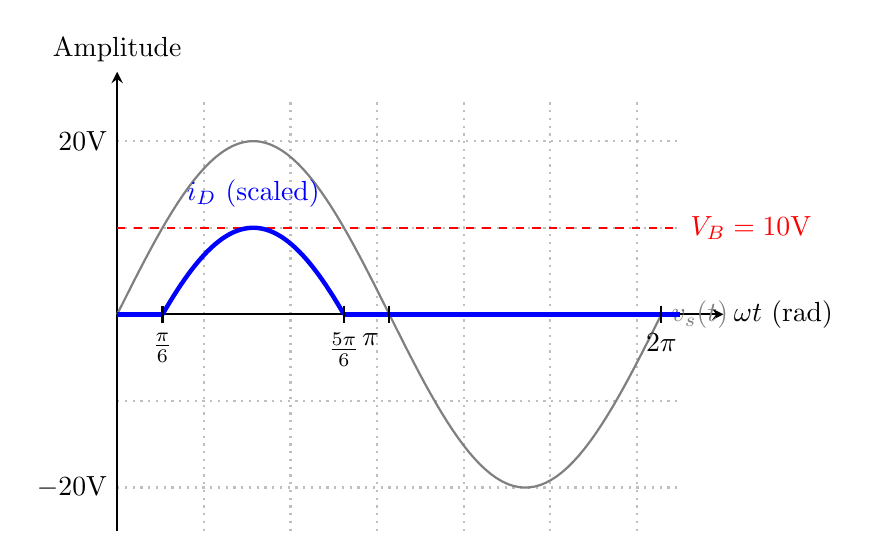
\begin{tikzpicture}[scale=1.1, >=stealth]
    % Grid
    \draw[dotted, gray!50] (0,-2.5) grid (6.5,2.5);
    
    % Axes
    \draw[->, thick] (0,0) -- (7,0) node[right] {$\omega t$ (rad)};
    \draw[->, thick] (0,-2.5) -- (0,2.8) node[above] {Amplitude};
    
    % Source Voltage (vs)
    \draw[thick, gray, domain=0:6.28, samples=100] plot (\x, {2*sin(\x*180/3.14159)}) node[right] {$v_s(t)$};
    
    % Battery Voltage level
    \draw[dashed, red, thick] (0,1) -- (6.5,1) node[right] {$V_B=10\text{V}$};
    
    % Diode Current (scaled for visibility)
    \draw[ultra thick, blue, domain=0.523:2.618, samples=50] plot (\x, {2*sin(\x*180/3.14159)-1});
    \draw[ultra thick, blue] (0,0) -- (0.523,0);
    \draw[ultra thick, blue] (2.618,0) -- (6.5,0);
    
    % Key points
    \draw (0.523,0.1) -- (0.523,-0.1) node[below] {$\frac{\pi}{6}$};
    \draw (2.618,0.1) -- (2.618,-0.1) node[below] {$\frac{5\pi}{6}$};
    \draw (3.141,0.1) -- (3.141,-0.1) node[below left] {$\pi$};
    \draw (6.283,0.1) -- (6.283,-0.1) node[below] {$2\pi$};
    
    % Labels
    \node[blue] at (1.57, 1.4) {$i_D$ (scaled)};
    \node[left] at (0, 2) {$20\text{V}$};
    \node[left] at (0, -2) {$-20\text{V}$};
\end{tikzpicture}
\end{center}

---

\subsection*{4. Final Answer Summary}

\begin{center}
\renewcommand{\arraystretch}{1.5}
\begin{tabular}{@{}llc@{}}
    \toprule
    \textbf{Parameter} & \textbf{Formula} & \textbf{Calculated Value} \\
    \midrule
    \textbf{Conduction Angle ($\theta_c$)} & $\pi - 2\arcsin(V_B/V_m)$ & $\frac{2\pi}{3}\text{ rad } (120^\circ)$ \\
    \textbf{Fraction of Cycle} & $\frac{\theta_c}{2\pi}$ & $\mathbf{1/3} \approx \mathbf{33.33\%}$ \\
    \textbf{Peak Diode Current} & $\frac{V_m - V_B}{R}$ & $\mathbf{100\text{ mA}}$ \\
    \textbf{Max Reverse Bias Voltage} & $V_m + V_B$ & $\mathbf{30\text{ V}}$ \\
    \bottomrule
\end{tabular}
\end{center}

\end{tcolorbox}

\end{enumerate}




\subtopic{cA}{Special Purpose Diodes/Thyristors}
\label{sub:s1-spd}

\begin{enumerate}
    
\item  Draw the circuit diagram of controlled full wave rectifier using SCR. Draw the waveforms of sinusoidal input, gate pulses and rectified output.
\mk{11.67} \yr{EEE 263 | L-2/T-1 | 2014--15}

\begin{tcolorbox}[enhanced,breakable,ansbox,colback=cA!4,colframe=cA,boxrule=0.8pt,arc=5pt,title={\textbf{Answer}},fonttitle=\bfseries\color{white},colbacktitle=cA]

\subsection*{1. Theory and Principle of Operation}
A controlled full-wave rectifier converts an alternating current (AC) input into a controlled direct current (DC) output using Silicon Controlled Rectifiers (SCRs) instead of standard diodes. The use of SCRs (thyristors) allows the user to control the output voltage magnitude by adjusting the firing angle ($\alpha$).

The most common configuration is the \textbf{Fully-Controlled Bridge Rectifier}, which utilizes four SCRs ($T_1$, $T_2$, $T_3$, $T_4$). 
\begin{itemize}
    \item \textbf{Positive Half-Cycle:} The top terminal of the AC source is positive. SCRs $T_1$ and $T_2$ are forward-biased. They begin to conduct only when a gate pulse is applied at $\omega t = \alpha$. Current flows from the source, through $T_1$, the load $R_L$, and returns via $T_2$.
    \item \textbf{Negative Half-Cycle:} The bottom terminal of the AC source is positive. SCRs $T_3$ and $T_4$ are forward-biased. They are triggered at $\omega t = \pi + \alpha$. Current flows through $T_3$, the load $R_L$ (in the same direction as before), and returns via $T_4$.
\end{itemize}
\textit{Assumption:} For the following analysis and waveforms, a purely resistive load ($R_L$) is assumed, meaning the output current becomes zero when the output voltage reaches zero at $\omega t = \pi, 2\pi, \dots$

---

\subsection*{2. Circuit Diagram}
\begin{center}
\begin{circuitikz}[thick, american, scale=1.1, transform shape]
    % AC Source
    \draw (-3, 2) to[sV, l=$v_s(t)$] (-3, -2);
    
    % AC lines to the bridge
    \draw (-3, 2) -- (0, 2);
    \fill (0,2) circle (1.5pt);
    \draw (-3, -2) -- (2, -2);
    \fill (2,-2) circle (1.5pt);
    
    % Bridge Leg 1 (Left)
    \draw (0, 2) to[Ty, l=$T_1$, *-*] (0, 4);
    \draw (0, -4) to[Ty, l=$T_4$, *-*] (0, 2);
    
    % Bridge Leg 2 (Right)
    \draw (2, -2) to[Ty, l=$T_3$, *-*] (2, 4);
    \draw (2, -4) to[Ty, l=$T_2$, *-*] (2, -2);
    
    % DC Output Rails
    \draw (0, 4) -- (5, 4);
    \draw (0, -4) -- (5, -4);
    
    % Load
    \draw (5, 4) to[R, l=$R_L$, v=$v_o(t)$, i>=$i_o$] (5, -4);
    
    % Output terminals (optional visual enhancement)
    \fill (5,4) circle (1.5pt);
    \fill (5,-4) circle (1.5pt);
    \node[above] at (5,4) {$+$};
    \node[below] at (5,-4) {$-$};
\end{circuitikz}
\end{center}

---

\subsection*{3. Waveforms}
The waveforms below illustrate the phase-control mechanism. A firing angle of $\alpha = 60^\circ$ ($\pi/3$) is shown for clarity.

\begin{center}
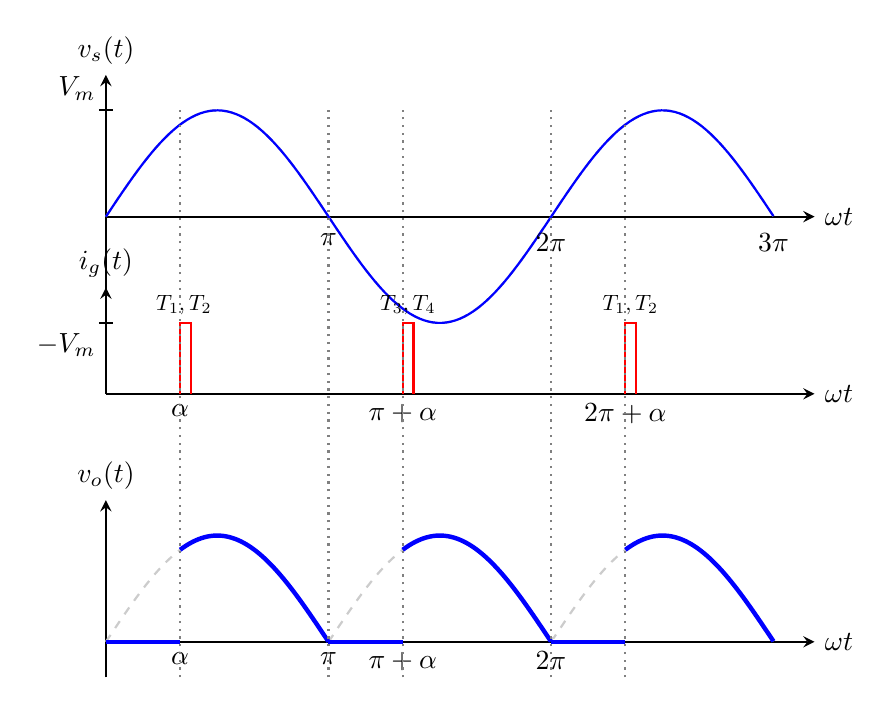
\begin{tikzpicture}[scale=0.9, >=stealth]
    
    \def\Vm{1.5}
    
    % ---------------------------------------------------
    % 1. Input Voltage
    % ---------------------------------------------------
    \begin{scope}[yshift=6cm]
        \draw[->, thick] (0,0) -- (10,0) node[right] {$\omega t$};
        \draw[->, thick] (0,-2) -- (0,2) node[above] {$v_s(t)$};
        
        % Sine wave
        \draw[thick, gray!60, dashed] plot[domain=0:9.42, samples=150] (\x, {\Vm*sin(\x*180/pi)});
        \draw[thick, blue] plot[domain=0:9.42, samples=150] (\x, {\Vm*sin(\x*180/pi)});
        
        \node[above left] at (0, \Vm) {$V_m$};
        \draw (-0.1, \Vm) -- (0.1, \Vm);
        \node[below left] at (0, -\Vm) {$-V_m$};
        \draw (-0.1, -\Vm) -- (0.1, -\Vm);
        
        \node[below] at (3.14, -0.1) {$\pi$};
        \node[below] at (6.28, -0.1) {$2\pi$};
        \node[below] at (9.42, -0.1) {$3\pi$};
    \end{scope}
    
    % ---------------------------------------------------
    % 2. Gate Trigger Pulses
    % ---------------------------------------------------
    \begin{scope}[yshift=3.5cm]
        \draw[->, thick] (0,0) -- (10,0) node[right] {$\omega t$};
        \draw[->, thick] (0,0) -- (0,1.5) node[above] {$i_g(t)$};
        
        % Pulse at alpha (pi/3 approx 1.047)
        \draw[thick, red] (1.047, 0) -- (1.047, 1) -- (1.2, 1) -- (1.2, 0);
        \node[above, scale=0.8] at (1.1, 1) {$T_1, T_2$};
        
        % Pulse at pi + alpha (4.188)
        \draw[thick, red] (4.188, 0) -- (4.188, 1) -- (4.34, 1) -- (4.34, 0);
        \node[above, scale=0.8] at (4.26, 1) {$T_3, T_4$};
        
        % Pulse at 2pi + alpha (7.33)
        \draw[thick, red] (7.33, 0) -- (7.33, 1) -- (7.48, 1) -- (7.48, 0);
        \node[above, scale=0.8] at (7.4, 1) {$T_1, T_2$};
        
        \node[below] at (1.047, 0) {$\alpha$};
        \node[below] at (4.188, 0) {$\pi+\alpha$};
        \node[below] at (7.33, 0) {$2\pi+\alpha$};
    \end{scope}
    
    % ---------------------------------------------------
    % 3. Output Voltage (Resistive Load)
    % ---------------------------------------------------
    \begin{scope}[yshift=0cm]
        \draw[->, thick] (0,0) -- (10,0) node[right] {$\omega t$};
        \draw[->, thick] (0,-0.5) -- (0,2) node[above] {$v_o(t)$};
        
        % Background reference
        \draw[gray!40, dashed, thick] plot[domain=0:9.42, samples=150] (\x, {abs(\Vm*sin(\x*180/pi))});
        
        % Output wave
        \draw[ultra thick, blue] (0,0) -- (1.047, 0);
        \draw[ultra thick, blue] plot[domain=1.047:3.14, samples=50] (\x, {\Vm*sin(\x*180/pi)});
        
        \draw[ultra thick, blue] (3.14, 0) -- (4.188, 0);
        \draw[ultra thick, blue] plot[domain=4.188:6.28, samples=50] (\x, {-\Vm*sin(\x*180/pi)});
        
        \draw[ultra thick, blue] (6.28, 0) -- (7.33, 0);
        \draw[ultra thick, blue] plot[domain=7.33:9.42, samples=50] (\x, {\Vm*sin(\x*180/pi)});
        
        \node[below] at (1.047, 0) {$\alpha$};
        \node[below] at (3.14, 0) {$\pi$};
        \node[below] at (4.188, 0) {$\pi+\alpha$};
        \node[below] at (6.28, 0) {$2\pi$};
    \end{scope}
    
    % Alignment Dashed Lines across all plots
    \draw[dotted, gray] (1.047, -0.5) -- (1.047, 7.5);
    \draw[dotted, gray] (3.14, -0.5) -- (3.14, 7.5);
    \draw[dotted, gray] (4.188, -0.5) -- (4.188, 7.5);
    \draw[dotted, gray] (6.28, -0.5) -- (6.28, 7.5);
    \draw[dotted, gray] (7.33, -0.5) -- (7.33, 7.5);
    
\end{tikzpicture}
\end{center}

---

\subsection*{4. Mathematical Derivation (Average DC Voltage)}
For a resistive load, conduction starts at $\omega t = \alpha$ and naturally ceases at $\omega t = \pi$ when the input voltage crosses zero. Because the waveform repeats every half-cycle (period of $\pi$), the average output voltage $V_{dc}$ is computed over one half-cycle:

\begin{align*}
    V_{dc} &= \frac{1}{\pi} \int_{\alpha}^{\pi} v_s(t) \, d(\omega t) \\
           &= \frac{1}{\pi} \int_{\alpha}^{\pi} V_m \sin(\omega t) \, d(\omega t) \\
           &= \frac{V_m}{\pi} \left[ -\cos(\omega t) \right]_{\alpha}^{\pi} \\
           &= \frac{V_m}{\pi} \Big( -\cos(\pi) - (-\cos(\alpha)) \Big) \\
           &= \frac{V_m}{\pi} \Big( -(-1) + \cos(\alpha) \Big) 
\end{align*}
\begin{equation}
    \therefore \quad \mathbf{V_{dc} = \frac{V_m}{\pi} (1 + \cos \alpha)}
\end{equation}

\subsection*{5. Important Notes}
\begin{itemize}
    \item \textbf{Control Range:} For a resistive load, the output voltage can be varied from maximum ($2V_m/\pi$ at $\alpha = 0^\circ$) to minimum ($0\text{ V}$ at $\alpha = 180^\circ$).
    \item \textbf{Highly Inductive Load:} If the load is highly inductive (like a DC motor), the load current becomes continuous. The SCRs continue to conduct past $\pi$ due to the energy stored in the inductor, until the next pair is triggered at $\pi + \alpha$. In that case, the integration limits change to $\alpha$ and $\pi+\alpha$, yielding the modified continuous-conduction equation: $V_{dc} = \frac{2V_m}{\pi} \cos \alpha$.
\end{itemize}

\end{tcolorbox}

\item Explain SCR and TRIAC operation with suitable examples.
\mk{15} \yr{EEE 263 | L-2/T-1 | 2013--14}

\begin{tcolorbox}[enhanced,breakable,ansbox,colback=cA!4,colframe=cA,boxrule=0.8pt,arc=5pt,title={\textbf{Answer}},fonttitle=\bfseries\color{white},colbacktitle=cA]

\subsection*{1. Introduction to Thyristors}

Thyristors are a class of multi-layered semiconductor devices designed for high-power switching applications. Operating purely as bistable switches (transitioning between a non-conducting \textbf{OFF} state and a highly conducting \textbf{ON} state), they are widely used in power electronics for phase control, AC/DC conversion, and power regulation. The most prominent members of this family are the \textbf{Silicon Controlled Rectifier (SCR)} and the \textbf{TRIAC}.

---

\subsection*{2. Silicon Controlled Rectifier (SCR)}

\subsubsection*{2.1 Structure and Operating Principle}
An SCR is a unidirectional, three-terminal, four-layer ($p$-$n$-$p$-$n$) semiconductor device. The three terminals are the \textbf{Anode ($A$)}, \textbf{Cathode ($K$)}, and \textbf{Gate ($G$)}. 

\begin{center}
    \begin{minipage}{0.45\textwidth}
        \centering
        \begin{circuitikz}[american, scale=0.9]
            % SCR Symbol
            \draw (0,0.8) to[thyristor, n=scr] (0,-1.2);
            \draw (scr.anode) -- (0,1.2) node[above] {Anode ($A$)};
            \draw (scr.cathode) -- (0,-1.6) node[below] {Cathode ($K$)};
            \draw (scr.gate) -- (-0.8,-0.8) node[left] {Gate ($G$)};
            \node[right=0.2cm] at (0,-0.2) {SCR Symbol};
        \end{circuitikz}
    \end{minipage}
    \hfill
    \begin{minipage}{0.45\textwidth}
        \centering
        \begin{circuitikz}[american, scale=0.8]
            % Transistors
            \draw (0,1.5) node[pnp] (Q1) {$Q_1$};
            \draw (2,-0.5) node[npn] (Q2) {$Q_2$};

            % Connections
            \draw (Q1.E) -- ++(0,0.5) node[above] {Anode ($A$)};
            \draw (Q2.E) -- ++(0,-0.5) node[below] {Cathode ($K$)};
            \draw (Q1.C) |- (Q2.B);
            \draw (Q2.C) |- (Q1.B);
            \draw (Q2.B) -- ++(-1.5,0) node[left] {Gate ($G$)};
            \node at (1,-2) {Two-Transistor Model};
        \end{circuitikz}
    \end{minipage}
\end{center}

An SCR operates in three primary modes:
\begin{enumerate}
    \item \textbf{Forward Blocking Mode (OFF State):} The Anode is biased positive relative to the Cathode ($V_{AK} > 0$), while the gate is left open ($I_G = 0$). Junctions $J_1$ and $J_3$ are forward-biased, but the middle junction $J_2$ is reverse-biased. Only a minuscule forward leakage current flows.
    \item \textbf{Forward Conduction Mode (ON State):} Conduction is initiated either by increasing $V_{AK}$ beyond the \textit{Forward Breakover Voltage} ($V_{BO}$) or, more practically, by applying a positive current pulse to the Gate ($I_G > 0$). This breaks down $J_2$ through regenerative feedback, driving the SCR into saturation. It remains in this state even after the gate signal is removed, provided the anode current stays above the \textit{Holding Current} ($I_H$).
    \item \textbf{Reverse Blocking Mode (OFF State):} The Cathode is positive relative to the Anode ($V_{AK} < 0$). Junctions $J_1$ and $J_3$ are reverse-biased, effectively blocking any current flow except for a tiny reverse leakage current.
\end{enumerate}

\subsubsection*{2.2 Mathematical Derivation: Two-Transistor Model}
The regenerative switching action can be analytically demonstrated using the two-transistor equivalent circuit shown above, which splits the $p$-$n$-$p$-$n$ structure into an interconnected $PNP$ transistor ($Q_1$) and an $NPN$ transistor ($Q_2$).

For $Q_1$, the collector current $I_{C1}$ is expressed as:
\begin{equation}
    I_{C1} = \alpha_1 I_A + I_{CBO1}
\end{equation}
where $\alpha_1$ is the common-base current gain of $Q_1$, $I_A$ is the anode current (emitter current of $Q_1$), and $I_{CBO1}$ is the reverse saturation current of the collector-base junction.

Similarly, for $Q_2$, the collector current $I_{C2}$ is:
\begin{equation}
    I_{C2} = \alpha_2 I_K + I_{CBO2}
\end{equation}
where $\alpha_2$ is the common-base current gain of $Q_2$, $I_K$ is the cathode current, and $I_{CBO2}$ is the corresponding reverse saturation current.

From Kirchhoff's Current Law (KCL) applied to the overall system:
\begin{equation}
    I_K = I_A + I_G
\end{equation}
The total anode current $I_A$ is the sum of the collector currents of both transistors:
\begin{equation}
    I_A = I_{C1} + I_{C2}
\end{equation}
Substituting equations (1) and (2) into (4):
\begin{equation}
    I_A = \alpha_1 I_A + I_{CBO1} + \alpha_2 I_K + I_{CBO2}
\end{equation}
Substituting $I_K = I_A + I_G$ into (5):
\begin{align*}
    I_A &= \alpha_1 I_A + I_{CBO1} + \alpha_2 (I_A + I_G) + I_{CBO2} \nonumber \\
    I_A(1 - \alpha_1 - \alpha_2) &= \alpha_2 I_G + I_{CBO1} + I_{CBO2}
\end{align*}
Solving for $I_A$:
\begin{equation}
    I_A = \frac{\alpha_2 I_G + I_{CBO1} + I_{CBO2}}{1 - (\alpha_1 + \alpha_2)}
\end{equation}

\textbf{Analysis of Latching Action:}
\begin{itemize}
    \item When $I_G = 0$, the low-current gains $\alpha_1$ and $\alpha_2$ are very small ($\alpha_1 + \alpha_2 \ll 1$). Consequently, $I_A$ is limited to a negligible leakage current, keeping the SCR \textbf{OFF}.
    \item When a positive gate current $I_G$ is injected, $I_{C2}$ increases, which in turn raises the base current of $Q_1$ ($I_{B1} = I_{C2}$). This increases $I_{C1}$, which further feeds back into the base of $Q_2$.
    \item Because the current gains $\alpha$ of BJTs increase with emitter current, this regenerative loop rapidly drives $(\alpha_1 + \alpha_2) \to 1$. As the denominator of equation (7) approaches zero, the anode current $I_A$ surges, limited only by the external load resistance. The SCR is now latched \textbf{ON}.
\end{itemize}

---

\subsubsection*{2.3 SCR Application Example: Phase-Controlled Half-Wave Rectifier}

Consider an SCR used in a single-phase half-wave rectifier circuit driving a resistive load $R_L = 10\ \Omega$. The AC input voltage source is $v_s(t) = 120\sqrt{2}\sin(120\pi t)\text{ V}$ (which corresponds to $120\text{ V}$ RMS at $60\text{ Hz}$). The SCR is fired at a constant delay angle $\alpha = 60^\circ$ ($\pi/3\text{ rad}$).

\begin{center}
    \begin{circuitikz}[american, scale=0.9]
        \draw (0,2) to[sV, l=$v_s(t)$] (0,0) -- (4,0);
        \draw (0,2) to[thyristor, n=S1, l=SCR] (2,2)
              to[R, l=$R_L$] (4,2) -- (4,0);
        \draw (S1.gate) -- ++(-0.2,-0.4) node[left] {Trigger Pulse ($\alpha$)};
    \end{circuitikz}
\end{center}

\textbf{Step 1: Determine the peak input voltage ($V_m$)}
\begin{equation*}
    V_m = 120\sqrt{2} \approx 169.73\text{ V}
\end{equation*}

\textbf{Step 2: Calculate the average (DC) output voltage ($V_{dc}$)}
The SCR conducts only from $\omega t = \alpha$ to $\pi$ during the positive half-cycle:
\begin{align*}
    V_{dc} &= \frac{1}{2\pi} \int_{\alpha}^{\pi} V_m \sin(\theta) d\theta = \frac{V_m}{2\pi} \Big[ -\cos\theta \Big]_{\alpha}^{\pi} \\
    V_{dc} &= \frac{V_m}{2\pi} (1 + \cos\alpha)
\end{align*}
Substituting $V_m = 169.73\text{ V}$ and $\alpha = 60^\circ$:
\begin{equation*}
    V_{dc} = \frac{169.73}{2\pi} (1 + \cos 60^\circ) = 27.01 \times (1 + 0.5) \approx \mathbf{40.52\text{ V}}
\end{equation*}

\textbf{Step 3: Calculate the RMS output voltage ($V_{rms}$)}
\begin{align*}
    V_{rms} &= \sqrt{\frac{1}{2\pi} \int_{\alpha}^{\pi} \left[V_m \sin(\theta)\right]^2 d\theta} = V_m \sqrt{\frac{1}{4\pi} \int_{\alpha}^{\pi} (1 - \cos 2\theta) d\theta} \\
    V_{rms} &= V_m \sqrt{\frac{1}{4\pi} \left[ \theta - \frac{\sin 2\theta}{2} \right]_{\alpha}^{\pi}} = V_m \sqrt{\frac{1}{4\pi} \left( \pi - \alpha + \frac{\sin 2\alpha}{2} \right)}
\end{align*}
Converting $\alpha = 60^\circ$ to radians ($\pi/3\text{ rad}$):
\begin{align*}
    V_{rms} &= 169.73 \sqrt{\frac{1}{4\pi} \left( \pi - \frac{\pi}{3} + \frac{\sin 120^\circ}{2} \right)} \\
    V_{rms} &= 169.73 \sqrt{\frac{1}{4\pi} \left( 2.0944 + 0.4330 \right)} \\
    V_{rms} &= 169.73 \sqrt{\frac{2.5274}{12.5664}} \approx 169.73 \times 0.4484 \approx \mathbf{76.11\text{ V}}
\end{align*}

\textbf{Step 4: Calculate the average power delivered to the load ($P_L$)}
\begin{equation*}
    P_L = \frac{V_{rms}^2}{R_L} = \frac{(76.11)^2}{10} \approx \mathbf{579.27\text{ W}}
\end{equation*}

---

\subsection*{3. TRIAC (Triode for Alternating Current)}

\subsubsection*{3.1 Structure and Operating Principle}
A TRIAC is a bidirectional, three-terminal semiconductor switch that can conduct current in both directions. It is structurally equivalent to two SCRs connected in an inverse-parallel (anti-parallel) configuration on a single silicon chip, sharing a common gate terminal. The main terminals are labeled \textbf{MT1} (Main Terminal 1, reference) and \textbf{MT2} (Main Terminal 2), along with the \textbf{Gate (G)}.

\begin{center}
    \begin{minipage}{0.45\textwidth}
        \centering
        \begin{circuitikz}[american, scale=0.9]
            % TRIAC Symbol
            \draw (0,0.8) to[triac, n=tri] (0,-1.2);
            \draw (0,0.8) -- (0,1.2) node[above] {Main Terminal 2 ($MT_2$)};
            \draw (0,-1.2) -- (0,-1.6) node[below] {Main Terminal 1 ($MT_1$)};
            \draw (tri.gate) -- (-0.8,-0.6) node[left] {Gate ($G$)};
            \node[right=0.2cm] at (0,-0.2) {TRIAC Symbol};
        \end{circuitikz}
    \end{minipage}
    \hfill
    \begin{minipage}{0.45\textwidth}
        \centering
        \begin{circuitikz}[american, scale=0.75]
            % Anti-parallel SCR Equivalent
            \draw (0,2) coordinate (top) -- (-1,2) to[thyristor, n=S1] (-1,-1) -- (0,-1) coordinate (bottom);
            \draw (top) -- (1,2) to[thyristor, n=S2, mirror] (1,-1) -- (bottom);
            \draw (top) -- (0,2.4) node[above] {$MT_2$};
            \draw (bottom) -- (0,-1.4) node[below] {$MT_1$};
            \draw (S1.gate) -- ++(-0.2,-0.2) node[left] {$G_1$};
            \draw (S2.gate) -- ++(0.2,-0.2) node[right] {$G_2$};
            \node at (0,-2.1) {Anti-Parallel SCR Equivalent};
        \end{circuitikz}
    \end{minipage}
\end{center}

Because of its unique multi-layered architecture, a TRIAC can be triggered into conduction by either a positive or negative gate current, regardless of the voltage polarity across $MT_2$ and $MT_1$. This allows operations in \textbf{four distinct quadrants}:

\begin{center}
\begin{tabular}{ccccc}
\toprule
\textbf{Quadrant} & \textbf{MT2 Voltage (w.r.t MT1)} & \textbf{Gate Voltage (w.r.t MT1)} & \textbf{Sensitivity} \\ \midrule
\textbf{I (+)}    & Positive ($>0$)                  & Positive ($>0$)                   & High (Easiest to trigger) \\
\textbf{I (-)}    & Positive ($>0$)                  & Negative ($<0$)                   & Medium \\
\textbf{III (-)}  & Negative ($<0$)                  & Negative ($<0$)                   & High \\
\textbf{III (+)}  & Negative ($<0$)                  & Positive ($>0$)                   & Low (Hardest to trigger) \\ \bottomrule
\end{tabular}
\end{center}

---

\subsubsection*{3.2 TRIAC Application Example: Full-Wave AC Phase Control (Light Dimmer)}

Consider a TRIAC installed in a domestic light dimmer circuit to control the power delivered to a resistive heating element $R_L = 10\ \Omega$. The AC supply voltage is $v_s(t) = 120\sqrt{2}\sin(120\pi t)\text{ V}$. The gate triggering circuit is configured to trigger the TRIAC symmetrically in both the positive and negative half-cycles at a firing angle $\alpha = 60^\circ$ ($\pi/3\text{ rad}$).

\begin{center}
    \begin{circuitikz}[american, scale=0.9]
        \draw (0,2) to[sV, l=$v_s(t)$] (0,0) -- (4,0);
        \draw (0,2) to[triac, n=T1, l=TRIAC] (2,2)
              to[R, l=$R_L$] (4,2) -- (4,0);
        \draw (T1.gate) -- ++(-0.2,-0.4) node[left] {Triggering Circuit};
    \end{circuitikz}
\end{center}

\textbf{Step 1: Calculate the RMS output voltage ($V_{rms}$)}
Unlike the SCR, which blocks the entire negative half-cycle, the TRIAC conducts symmetrically in both half-cycles. Thus, the mean-square value is evaluated over a single half-cycle ($\pi$ radians):
\begin{align*}
    V_{rms} &= \sqrt{\frac{1}{\pi} \int_{\alpha}^{\pi} \left[V_m \sin(\theta)\right]^2 d\theta} = V_m \sqrt{\frac{1}{2\pi} \int_{\alpha}^{\pi} (1 - \cos 2\theta) d\theta} \\
    V_{rms} &= V_m \sqrt{\frac{1}{2\pi} \left( \pi - \alpha + \frac{\sin 2\alpha}{2} \right)}
\end{align*}
Comparing this expression with the SCR half-wave RMS voltage shows:
\begin{equation*}
    V_{rms,\text{TRIAC}} = \sqrt{2} \times V_{rms,\text{SCR}}
\end{equation*}
Substituting the values calculated previously:
\begin{equation*}
    V_{rms} = 169.73 \sqrt{\frac{2.5274}{2\pi}} = 169.73 \sqrt{0.4022} \approx 169.73 \times 0.6342 \approx \mathbf{107.64\text{ V}}
\end{equation*}

\textbf{Step 2: Calculate the average power delivered to the load ($P_L$)}
\begin{equation*}
    P_L = \frac{V_{rms}^2}{R_L} = \frac{(107.64)^2}{10} \approx \mathbf{1158.64\text{ W}}
\end{equation*}

\textit{Note: Controlling power with a TRIAC provides exactly double the load power of a single SCR at the same firing angle because both half-cycles are utilized.}

---

\subsection*{4. Comparison: SCR vs. TRIAC}

\begin{center}
\begin{tabular}{lll}
\toprule
\textbf{Feature} & \textbf{SCR} & \textbf{TRIAC} \\ \midrule
\textbf{Directionality} & Unidirectional (DC current flow) & Bidirectional (AC current flow) \\
\textbf{Terminals} & Anode, Cathode, Gate & Main Terminal 1, Main Terminal 2, Gate \\
\textbf{Gate Triggering} & Positive pulse only (with positive $V_{AK}$) & Positive or negative pulse \\
\textbf{Power Rating} & Very High (up to several thousand Amperes) & Moderate to Medium ($< 100\text{ A}$ typical) \\
\textbf{Symmetry} & Asymmetric control & Symmetric control over full AC cycles \\
\textbf{Common Applications} & Controlled rectifiers, High-voltage DC transmission & Light dimmers, fan regulators, AC motor drives \\ \bottomrule
\end{tabular}
\end{center}

\end{tcolorbox}

\item Sketch the output wave form of the following circuit given in Fig. for Q. 1(c)(i) assuming output wave is obtained across the resistance. The input waveform and gate pulse sequence is given in Fig. for Q. 1(c)(ii). 

\subsection*{1. Circuit Diagram [Fig. 1(c)(i)]}
\begin{center}
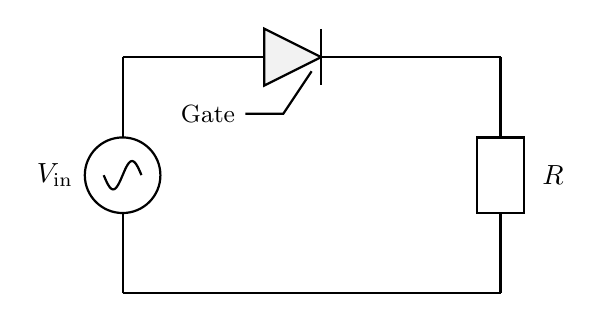
\begin{tikzpicture}[thick,scale=1.2, thick]
    % Bottom connection wire
    \draw (0,0) -- (4,0);
    
    % Left side: AC Input Voltage Source (Manual Draw)
    \draw (0,0) -- (0,0.85);
    \draw (0,1.25) circle (0.4cm);
    % Sine wave inside the circle
    \draw[smooth, samples=50, domain=-0.2:0.2] plot (\x, {1.25 + 0.15*sin(\x*360/0.4)});
    \node[left=0.5cm] at (0,1.25) {$V_{\text{in}}$};
    \draw (0,1.65) -- (0,2.5);
    
    % Top wire to SCR
    \draw (0,2.5) -- (1.5,2.5);
    
    % --- Pure TikZ SCR Symbol (Centered at x=1.85) ---
    % Diode Triangle
    \draw[fill=black!5] (1.5,2.8) -- (1.5,2.2) -- (2.1,2.5) -- cycle;
    % Cathode Bar
    \draw (2.1,2.8) -- (2.1,2.2);
    % Gate Terminal (Coming out diagonally from cathode side)
    \draw (2.0,2.35) -- (1.7,1.9) -- (1.3,1.9) node[left, font=\small] {Gate};
    
    % Wire from SCR to Resistor
    \draw (2.1,2.5) -- (4,2.5);
    
    % Right side: Load Resistor (Standard Rectangle for 100% compatibility)
    \draw (4,2.5) -- (4,1.65);
    \draw (3.75,1.65) rectangle (4.25,0.85);
    \node[right=0.4cm] at (4,1.25) {$R$};
    \draw (4,0.85) -- (4,0);
\end{tikzpicture}
\end{center}

\subsection*{2. Input Voltage Waveform [Fig. 1(c)(ii)]}
\begin{center}
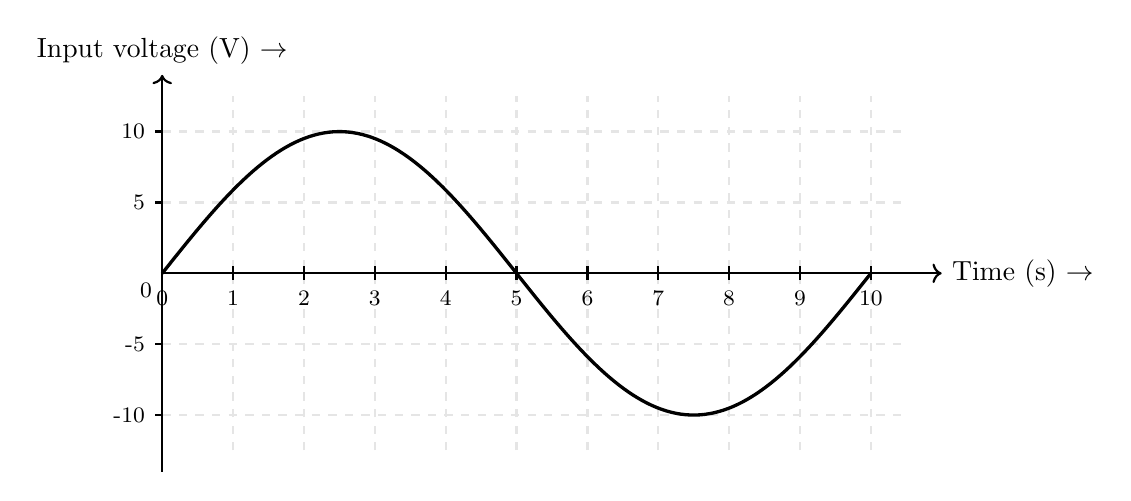
\begin{tikzpicture}[thick,scale=0.9]
    % Grid lines (dashed, light gray)
    \draw[step=1cm, gray!20, dashed] (0,-2.5) grid (10.5,2.5);

    % Axes
    \draw[->, thick] (0,0) -- (11,0) node[right] {Time (s) $\rightarrow$};
    \draw[->, thick] (0,-2.8) -- (0,2.8) node[above] {Input voltage (V) $\rightarrow$};
    
    % X-axis Ticks and Labels (0 to 10)
    \foreach \x in {0,1,...,10} {
        \draw (\x,0.1) -- (\x,-0.1);
        \node[below, font=\footnotesize] at (\x,-0.1) {\x};
    }
    
    % Y-axis Ticks and Labels (-10, -5, 5, 10) -> Scaled: 1 unit = 5V
    \draw (0,1) -- (-0.1,1) node[left, font=\footnotesize] {5};
    \draw (0,2) -- (-0.1,2) node[left, font=\footnotesize] {10};
    \draw (0,-1) -- (-0.1,-1) node[left, font=\footnotesize] {-5};
    \draw (0,-2) -- (-0.1,-2) node[left, font=\footnotesize] {-10};
    \node[below left, font=\footnotesize] at (0,0) {0};

    % Sine Wave Plotting: Max amplitude 10V (mapped to 2 units on Y)
    % One full cycle (2*pi) spans from x=0 to x=10
    \draw[very thick, black] plot[domain=0:10, samples=150] (\x, {2*sin(\x*360/10)});
\end{tikzpicture}
\end{center}

\vspace{1cm}

\subsection*{3. Gate Pulse Sequence [Fig. 1(c)(ii)]}
\begin{center}
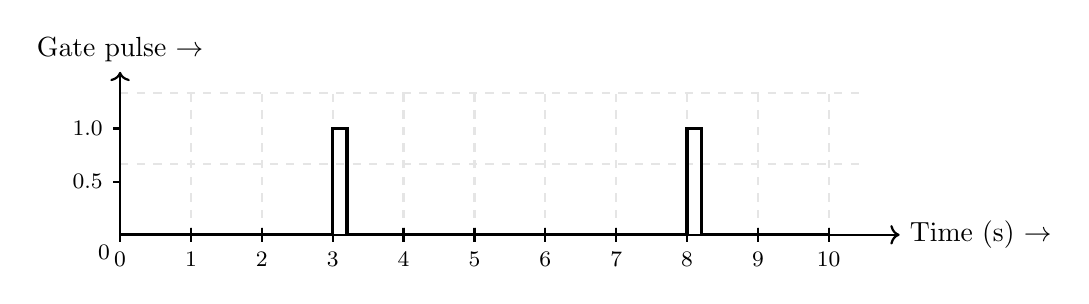
\begin{tikzpicture}[thick,scale=0.9]
    % Grid lines
    \draw[step=1cm, gray!20, dashed] (0,0) grid (10.5,2);

    % Axes
    \draw[->, thick] (0,0) -- (11,0) node[right] {Time (s) $\rightarrow$};
    \draw[->, thick] (0,0) -- (0,2.3) node[above] {Gate pulse $\rightarrow$};
    
    % X-axis Ticks and Labels
    \foreach \x in {0,1,...,10} {
        \draw (\x,0.1) -- (\x,-0.1);
        \node[below, font=\footnotesize] at (\x,-0.1) {\x};
    }
    
    % Y-axis Ticks and Labels
    \draw (0,0.75) -- (-0.1,0.75) node[left, font=\footnotesize] {0.5};
    \draw (0,1.5) -- (-0.1,1.5) node[left, font=\footnotesize] {1.0};
    \node[below left, font=\footnotesize] at (0,0) {0};

    % Drawing the pulse sequence (Triggers at t=3 and t=8)
    % Height is 1.5 units (representing 1.0V or logic high)
    \draw[very thick, black] (0,0) -- (3,0) 
                          -- (3,1.5) -- (3.2,1.5) -- (3.2,0) 
                          -- (8,0) 
                          -- (8,1.5) -- (8.2,1.5) -- (8.2,0) 
                          -- (10,0);
\end{tikzpicture}
\end{center}

\mk{20} \yr{EEE 263 | L-2/T-1 | 2011--12}


\begin{tcolorbox}[enhanced,breakable,ansbox,colback=cA!4,colframe=cA,boxrule=0.8pt,arc=5pt,title={\textbf{Answer}},fonttitle=\bfseries\color{white},colbacktitle=cA]

\subsection*{1. Operating Principle of the SCR Circuit}

To determine the output voltage waveform across the load resistance $R$, we must analyze the state of the Silicon Controlled Rectifier (SCR) across different intervals of the input cycle. 

The input voltage waveform is given by:
\begin{equation}
    V_{\text{in}}(t) = V_m \sin(\omega t) = 10 \sin\left(\frac{2\pi}{T} t\right) \text{ V}
\end{equation}
Given that one full cycle of the input sine wave has a period of $T = 10\text{ s}$, the angular frequency is $\omega = \frac{2\pi}{10} = 0.2\pi\text{ rad/s}$. Thus:
\begin{equation}
    V_{\text{in}}(t) = 10 \sin(0.2\pi t) \text{ V}
\end{equation}

For an SCR to switch from the non-conducting (\textbf{OFF}) state to the conducting (\textbf{ON}) state, two conditions must be satisfied simultaneously:
\begin{enumerate}
    \item The SCR must be \textbf{forward-biased}, meaning the anode is positive relative to the cathode ($V_{\text{AK}} > 0 \implies V_{\text{in}} > 0$).
    \item A positive triggering pulse must be applied to the \textbf{gate} terminal ($I_G > 0$).
\end{enumerate}

Once triggered, the SCR remains \textbf{ON} (even if the gate pulse is removed) until its anode current falls below the holding current ($I_H$), which in an AC circuit occurs when the input voltage goes to zero and reverses polarity (known as \textbf{natural/line commutation}).

---

\subsection*{2. Interval-by-Interval Analysis}

\subsubsection*{Interval 1: $0\text{ s} \le t < 3\text{ s}$}
\begin{itemize}
    \item The input voltage is positive ($V_{\text{in}} > 0$), which means the SCR is forward-biased.
    \item However, no gate pulse is applied ($I_G = 0$).
    \item Consequently, the SCR remains in the \textbf{Forward Blocking State (OFF)}.
    \item The output voltage across the resistor is:
    \begin{equation}
        V_{\text{out}}(t) = 0\text{ V}
    \end{equation}
\end{itemize}

\subsubsection*{At $t = 3\text{ s}$ (Firing Instant)}
\begin{itemize}
    \item The input voltage at this instant is:
    \begin{equation}
        V_{\text{in}}(3) = 10 \sin(0.2\pi \times 3) = 10 \sin(108^\circ) \approx 9.51\text{ V} > 0
    \end{equation}
    Since $V_{\text{in}}(3) > 0$, the SCR is forward-biased.
    \item At this exact instant, a gate pulse is applied.
    \item Since both conditions (forward bias and gate trigger) are met, the SCR triggers \textbf{ON} instantly. 
    \item Assuming an ideal SCR with a negligible forward voltage drop ($V_F = 0\text{ V}$), the voltage across the SCR drops to $0\text{ V}$. The output voltage instantly jumps from $0\text{ V}$ to the input voltage:
    \begin{equation}
        V_{\text{out}}(3) \approx 9.51\text{ V}
    \end{equation}
\end{itemize}

\subsubsection*{Interval 2: $3\text{ s} \le t < 5\text{ s}$}
\begin{itemize}
    \item The SCR remains in the \textbf{Forward Conduction State (ON)}.
    \item The output voltage follows the input voltage profile:
    \begin{equation}
        V_{\text{out}}(t) = V_{\text{in}}(t) = 10 \sin(0.2\pi t) \text{ V}
    \end{equation}
    \item Note that since the peak of the input voltage ($10\text{ V}$) occurred at $t = 2.5\text{ s}$ (while the SCR was still OFF), the output voltage starts at $9.51\text{ V}$ at $t = 3\text{ s}$ and decreases continuously following the sinusoidal path down to $0\text{ V}$ at $t = 5\text{ s}$.
\end{itemize}

\subsubsection*{At $t = 5\text{ s}$ (Natural Commutation)}
\begin{itemize}
    \item The input voltage becomes zero ($V_{\text{in}} = 0\text{ V}$) and begins to transition to negative values.
    \item The anode current drops to zero (below the holding current $I_H$), causing the SCR to turn \textbf{OFF} naturally.
\end{itemize}

\subsubsection*{Interval 3: $5\text{ s} \le t < 8\text{ s}$}
\begin{itemize}
    \item The input voltage is negative ($V_{\text{in}} < 0$), putting the SCR in a reverse-biased condition.
    \item No gate pulse is applied.
    \item The SCR remains in the \textbf{Reverse Blocking State (OFF)}.
    \item The output voltage is:
    \begin{equation}
        V_{\text{out}}(t) = 0\text{ V}
    \end{equation}
\end{itemize}

\subsubsection*{At $t = 8\text{ s}$ (Gate Pulse under Reverse Bias)}
\begin{itemize}
    \item A gate pulse is applied at $t = 8\text{ s}$.
    \item However, the input voltage at this instant is negative:
    \begin{equation}
        V_{\text{in}}(8) = 10 \sin(0.2\pi \times 8) = 10 \sin(288^\circ) \approx -9.51\text{ V} < 0
    \end{equation}
    \item Since the SCR is reverse-biased, the gate pulse cannot trigger the device. The SCR remains in the \textbf{Reverse Blocking State (OFF)}.
    \item The output voltage remains at:
    \begin{equation}
        V_{\text{out}}(8) = 0\text{ V}
    \end{equation}
\end{itemize}

\subsubsection*{Interval 4: $8\text{ s} \le t \le 10\text{ s}$}
\begin{itemize}
    \item The input voltage finishes its negative half-cycle and goes back to zero.
    \item The SCR remains \textbf{OFF}.
    \item The output voltage is:
    \begin{equation}
        V_{\text{out}}(t) = 0\text{ V}
    \end{equation}
\end{itemize}

---

\subsection*{3. Output Voltage Waveform Sketch}

The derived mathematical definition of the output voltage is:
\begin{equation}
    V_{\text{out}}(t) = 
    \begin{cases} 
        0\text{ V} & 0\text{ s} \le t < 3\text{ s} \\
        10 \sin(0.2\pi t) \text{ V} & 3\text{ s} \le t < 5\text{ s} \\
        0\text{ V} & 5\text{ s} \le t \le 10\text{ s}
    \end{cases}
\end{equation}

Below is the sketch of the output waveform across the load resistor $R$.

\begin{center}
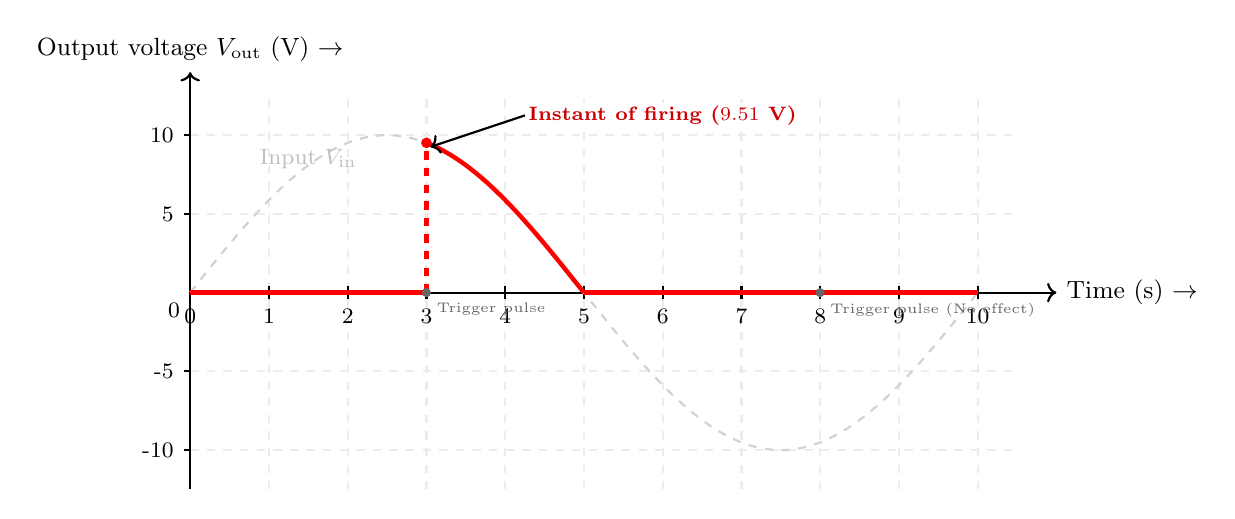
\begin{tikzpicture}[thick, scale=1.0]
    % Grid lines (dashed, light gray)
    \draw[step=1cm, gray!15, dashed] (0,-2.5) grid (10.5,2.5);

    % Axes
    \draw[->, thick] (0,0) -- (11,0) node[right, font=\small] {Time (s) $\rightarrow$};
    \draw[->, thick] (0,-2.5) -- (0,2.8) node[above, font=\small] {Output voltage $V_{\text{out}}$ (V) $\rightarrow$};
    
    % X-axis Ticks and Labels (0 to 10)
    \foreach \x in {0,1,...,10} {
        \draw (\x,0.08) -- (\x,-0.08);
        \node[below, font=\footnotesize] at (\x,-0.08) {\x};
    }
    
    % Y-axis Ticks and Labels (Scaled: 1 unit = 5V)
    \draw (0,1) -- (-0.08,1) node[left, font=\footnotesize] {5};
    \draw (0,2) -- (-0.08,2) node[left, font=\footnotesize] {10};
    \draw (0,-1) -- (-0.08,-1) node[left, font=\footnotesize] {-5};
    \draw (0,-2) -- (-0.08,-2) node[left, font=\footnotesize] {-10};
    \node[below left, font=\footnotesize] at (0,0) {0};

    % Reference lightly dashed input sine wave
    \draw[gray!35, dashed, domain=0:10, samples=150] plot (\x, {2*sin(\x*36)});
    \node[gray!50, font=\footnotesize] at (1.5,1.7) {Input $V_{\text{in}}$};

    % Plotting the output waveform V_out in red
    % Interval 0 to 3: V_out = 0V
    \draw[ultra thick, red] (0,0) -- (3,0);
    
    % Sudden jump at t = 3s to 9.51V (represented as 9.51/5 = 1.902 units)
    \draw[ultra thick, red, dashed] (3,0) -- (3,1.902);
    
    % Interval 3 to 5: V_out follows the input sine wave
    \draw[ultra thick, red, domain=3:5, samples=100] plot (\x, {2*sin(\x*36)});
    
    % Interval 5 to 10: V_out = 0V
    \draw[ultra thick, red] (5,0) -- (10,0);
    
    % Key point labels
    \filldraw[red] (3,1.902) circle (1.5pt);
    \draw[<-] (3.05, 1.85) -- ++(1.2, 0.4) node[right, fill=white, inner sep=1pt, font=\scriptsize\bfseries\color{red!80!black}] {Instant of firing ($9.51\text{ V}$)};
    
    \filldraw[black!60] (3,0) circle (1.2pt);
    \node[below right, font=\tiny\color{black!60}] at (3,0) {Trigger pulse};
    
    \filldraw[black!60] (8,0) circle (1.2pt);
    \node[below right, font=\tiny\color{black!60}] at (8,0) {Trigger pulse (No effect)};
\end{tikzpicture}
\end{center}

\end{tcolorbox}                                                                                                                                                                                                                                                                                                                                                                                                                                                                                                                                                                                                                                                                                                                                                                                                                                                                                                                                                                                                                                                                                                                                                                                                                                                                                                                                                                                                                                                                                                                                                                                                                                                                                                                                                                                                                                                                                                                                                                                                                                                                                                                                                                                                                                                                                                                                                                                                                                                                                                                                                                                                                                                                                                                                                                                                                                                                                                                                                                                                                                                                                                                                                                                                                                                                                                                                                                                                                                                                                                                                                                                                                                                                                                                                                                                                                                                                                                                                                                                                                                                                                                                                                                                                                                                                                                                                                                                                                                                                                                                                                                                                                                                                                                                                                                                                                                                                                                                                                                                                                                                                                                                                                                                                                                                                                                                                                                                                                                                                                                                                                                                                                                                                                                                                                                                                                                                                                                                                                                                                                                                                                                                                                                                                                                                                                                                                                                                                                                                                                                                                                                                                                                                                                                                                                                                                                                                                                                                                                                                                                                                                                                                                                                                                                                                                                                                                                                                                                                                                                                                                                                                                                                                                                                                                                                                                                                                                                                                                                                                                                                                                                                                                                                                                                                                                                                                                                                                                                                                                                                                                                                                                                                                                                                                                                                                                                                                                                                                                                                                                                                                                                                                                                                                                                                                                                                                                                                                                                                                                                                                                                                                                                                                                                                                                                                                                                                                                                                                                                                                                                                                                                                                                                                                                                                                                                                                                                                                                                                                                                                                                                                                                                                                                                                                                                                                                                                                                                                                                                                                                                                                                                                                                                                                                                                                                                                                                                                                                                                                                                                                                                                                                                                                                                                                                                                                                                                                                                                                                                                                                                                                                                                                                                                                                                                                                                                                                                                                                                                                                                                                                                                                                                                                                                                                                                                                                                                                                                                                                                                                                                                                                                                                                                                                                                                                                                                                                                                                                                                                                                                                                                                                                                                                                                                                                                                                                                                                                                                                                                                                                                                                                                                                                                                                                                                                                                                                                                                                                                                                                                                                                                                                                                                                                                                                                                                                                                                                                                                                                                                                                                                                                                                                                                                                                                                                                                                                                                                                                                                                                                                                                                                                                                                                                                                                                                                                                                                                                                                                                                                                                                                                                                                                                                                                                                                                                                                                                                                                                                                                                                                                                                                                                                                                                                                                                                                                                                                                                                                                                                                                                                                                                                                                                                                                                                                                                                                                                                                                                                                                                                                                                                                                                                                                                                                                                                                                                                                                                                                                                                                                                                                                                                                                                                                                                                                                                                                                                                                                                                                                                                                                                                                                                                                                                                                                                                                                                                                                                                                                                                                                                                                                                                                                                                                                                                                                                                                                                                                                                                                                                                                                                                                                                                                                                                                                                                                                                                                                                                                                                                                                                                                                                                                                                                                                                                                                                                                                                                                                                                                                                                                                                                                                                                                                                                                                                                                                                                                                                                                                                                                                                                                                                                                                                                                                                                                                                                                                                                                                                                                                                                                                                                                                                                                                                                                                                                                                                                                                                                                                                                                                                                                                                                                                                                                                                                                                                                                                                                                                                                                                                                                                                                                                                                                                                                                                                                                                                                                                                                                                                                                                                                                                                                                                                                                                                                                                                                                                                                                                                                                                                                                                                                                                                                                                                                                                                                                                                                                                                                                                                                                                                                                                                                                                                                                                                                                                                                                                                                                                                                                                                                                                                                                                                                                                                                                                                                                                                                                                                                                                                                                                                                                                                                                                                                                                                                                                                                                                                                                                                                                                                                                                                                                                                                                                                                                                                                                                                                                                                                                                                                                                                                                                                                                                                                                                                                                                                                                                                                                                                                                                                                                                                                                                                                                                                                                                                                                                                                                                                                                                                                                                                                                                                                                                                                                                                                                                                                                                                                                                                                                                                                                                                                                                                                                                                                                                                                                                                                                                                                                                                                                                                                                                                                                                                                                                                                                                                                                                                                                                                                                                                                                                                                                                                                                                                                                                                                                                                                                                                                                                                                                                                                                                                                                                                                                                                                                                                                                                                                                                                                                                                                                                                                                                                                                                                                                                                                                                                                                                                                                                                                                                                                                                                                                                                                                                                                                                                                                                                                                                                                                                                                                                                                                                                                                                                                                                                                                                                                                                                                                                                                                                                                                                                                                                                                                                                                                                                                                                                                                                                                                                                                                                                                                                                                                                                                                                                                                                                                                                                                                                                                                                                                                                                                                                                                                                                                                                                                                                                                                                                                                                                                                                                                                                                                                                                                                                                                                                                                                                                                                                                                                                                                                                                                                                                                                                                                                                                                                                                                                                                                                                                                                                                                                                                                                                                                                                                                                                                                                                                                                                                                                                                                                                                                                                                                                                                                                                                                                                                                                                                                                                                                                                                                                                                                                                                                                                                                                                                                                                                                                                                                                                                                                                                                                                                                                                                                                                                                                                                                                                                                                                                                                                                                                                                                                                                                                                                                                                                                                                                                                                                                                                                                                                                                                                                                                                                                                                                                                                                                                                                                                                                                                                                                                                                                                                                                                                                                                                                                                                                                                                                                                                                                                                                                                                                                                                                                                                                                                                                                                                                                                                                                                                                                                                                                                                                                                                                                                                                                                                                                                                                                                                                                                                                                                                                                                                                                                                                                     

\item Draw the I-V characteristics of an SCR and a TRIAC.
\mk{10} \yr{EEE 263 | L-2/T-1 | 2011--12}

\begin{tcolorbox}[enhanced,breakable,ansbox,colback=cA!4,colframe=cA,boxrule=0.8pt,arc=5pt,title={\textbf{Answer}},fonttitle=\bfseries\color{white},colbacktitle=cA]

\section*{1. Silicon Controlled Rectifier (SCR)}

\subsection*{1.1 Overview and Operating Principle}
The Silicon Controlled Rectifier (SCR) is a four-layer ($p\text{-}n\text{-}p\text{-}n$), three-junction, three-terminal unidirectional semiconductor device. The three terminals are the Anode (A), Cathode (K), and Gate (G). It acts as a controlled switch that permits conduction only in the forward direction (from Anode to Cathode) once triggered by a positive gate current pulse.

\begin{center}
  \begin{circuitikz}[scale=1.2]
    \draw (0,0) to[thyristor, name=scr] (2.5,0);
    \node[left] at (0,0) {Anode (A)};
    \node[right] at (2.5,0) {Cathode (K)};
    \draw (scr.gate) -- ++(-0.2,-0.6) node[below] {Gate (G)};
  \end{circuitikz}
  \captionof{figure}{Schematic Symbol of a Silicon Controlled Rectifier (SCR)}
\end{center}

\subsection*{1.2 I-V Characteristics of an SCR}
The current-voltage ($I\text{-}V$) relationship of an SCR consists of three main regions of operation:
\begin{enumerate}
    \item \textbf{Forward Blocking Region ($0 < V_{AK} < V_{BO}$ with $I_G = 0$):} The anode is positive relative to the cathode, but since no gate current is applied, the device remains in an OFF state, allowing only a small forward leakage current to flow.
    \item \textbf{Forward Conduction Region ($V_{AK} > V_H$):} Once the anode-to-cathode voltage exceeds the forward breakover voltage ($V_{BO}$) or a gate current pulse ($I_G$) is applied, the SCR switches to its ON state. The voltage drop across the device falls to a very low value (holding voltage, $V_H \approx 1\text{ to }1.5\text{ V}$), and the current is limited only by the external load resistance.
    \item \textbf{Reverse Blocking Region ($-V_{BR} < V_{AK} < 0$):} When the cathode is positive relative to the anode, junctions $J_1$ and $J_3$ are reverse-biased. The device remains OFF and permits only a tiny reverse leakage current.
    \item \textbf{Reverse Breakdown Region ($V_{AK} < -V_{BR}$):} If the reverse voltage exceeds the critical reverse breakdown voltage ($V_{BR}$), avalanching occurs, leading to a rapid increase in reverse current and potential device failure if not externally limited.
\end{enumerate}

\begin{center}
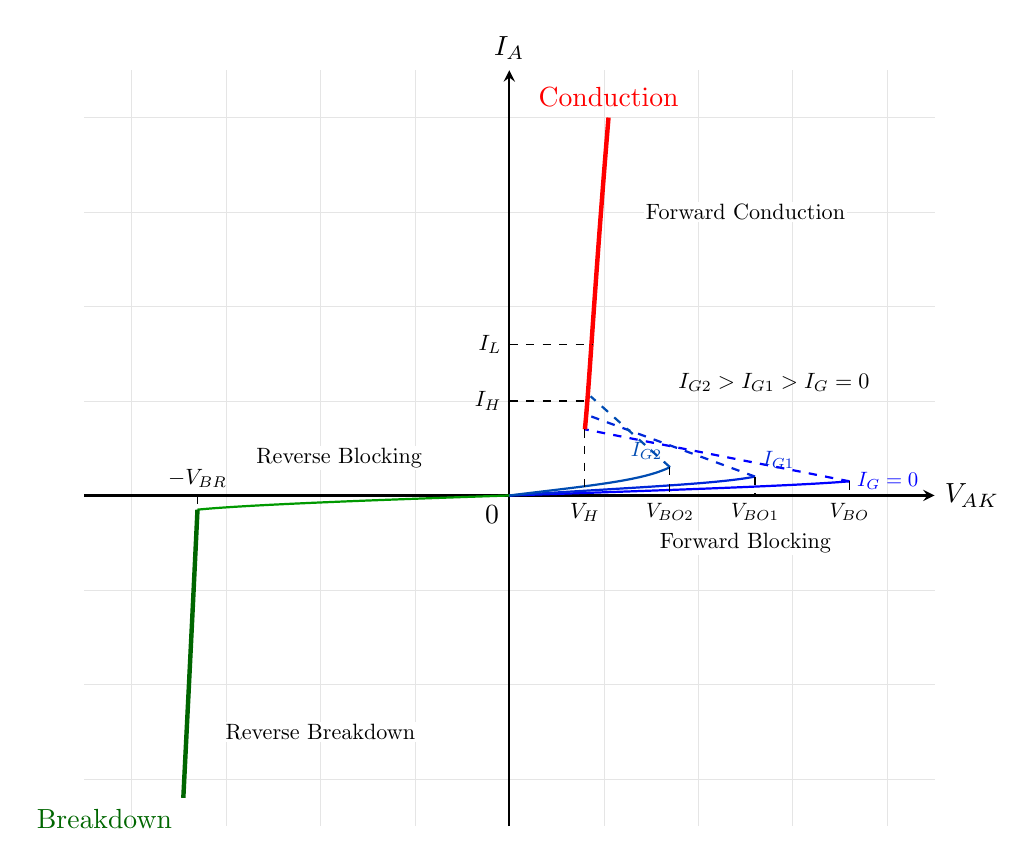
\begin{tikzpicture}[scale=1.2]
  % Grid
  \draw[very thin, gray!20] (-4.5,-3.5) grid (4.5,4.5);
  
  % Axes
  \draw[->, >=stealth, thick] (-4.5,0) -- (4.5,0) node[right] {$V_{AK}$};
  \draw[->, >=stealth, thick] (0,-3.5) -- (0,4.5) node[above] {$I_A$};
  
  % Origin
  \node[below left] at (0,0) {$0$};

  % --- QUADRANT I: FORWARD DIRECTION ---
  % IG0 = 0
  \draw[thick, blue] (0,0) .. controls (1.5,0.05) and (3.0,0.1) .. (3.6,0.15) node[right, scale=0.75] {$I_G = 0$};
  \draw[dashed, blue] (3.6,0.15) -- (0.8,0.7);
  \draw[dashed, thin, black] (3.6,0.15) -- (3.6,0) node[below, scale=0.75] {$V_{BO}$};
  
  % IG1 > 0
  \draw[thick, blue!70!teal] (0,0) .. controls (1.2,0.08) and (2.2,0.12) .. (2.6,0.2) node[above right, scale=0.75] {$I_{G1}$};
  \draw[dashed, blue!70!teal] (2.6,0.2) -- (0.83,0.85);
  \draw[dashed, thin, black] (2.6,0.2) -- (2.6,0) node[below, scale=0.75] {$V_{BO1}$};

  % IG2 > IG1
  \draw[thick, blue!40!teal] (0,0) .. controls (0.8,0.1) and (1.4,0.15) .. (1.7,0.3) node[above left, scale=0.75] {$I_{G2}$};
  \draw[dashed, blue!40!teal] (1.7,0.3) -- (0.86,1.05);
  \draw[dashed, thin, black] (1.7,0.3) -- (1.7,0) node[below, scale=0.75] {$V_{BO2}$};
  
  % Gate current relationship
  \node[scale=0.8, align=left] at (2.8,1.2) {$I_{G2} > I_{G1} > I_G=0$};

  % Forward Conduction
  \draw[ultra thick, red] (0.8,0.7) .. controls (0.85,1.2) and (0.9,2.2) .. (1.05,4.0) node[above] {Conduction};
  
  % Latching & Holding Current Labels
  \draw[dashed, thin] (0,1.0) node[left, scale=0.8] {$I_H$} -- (0.85,1.0);
  \draw[dashed, thin] (0,1.6) node[left, scale=0.8] {$I_L$} -- (0.88,1.6);
  
  % Holding voltage
  \draw[dashed, thin] (0.8,0.7) -- (0.8,0) node[below, scale=0.8] {$V_H$};

  % --- QUADRANT III: REVERSE DIRECTION ---
  % Reverse Blocking
  \draw[thick, green!60!black] (0,0) .. controls (-1.5,-0.05) and (-2.8,-0.1) .. (-3.3,-0.15);
  % Reverse Breakdown
  \draw[ultra thick, green!40!black] (-3.3,-0.15) .. controls (-3.35,-1.2) and (-3.4,-2.2) .. (-3.45,-3.2) node[below left] {Breakdown};
  \draw[dashed, thin] (-3.3,0) node[above, scale=0.8] {$-V_{BR}$} -- (-3.3,-0.15);
  
  % Region Labels
  \node[scale=0.8, fill=white, inner sep=1pt] at (2.5,-0.5) {Forward Blocking};
  \node[scale=0.8, fill=white, inner sep=1pt] at (-1.8,0.4) {Reverse Blocking};
  \node[scale=0.8, fill=white, inner sep=1pt] at (2.5,3.0) {Forward Conduction};
  \node[scale=0.8, fill=white, inner sep=1pt] at (-2.0,-2.5) {Reverse Breakdown};
\end{tikzpicture}
\captionof{figure}{I-V Characteristics of a Silicon Controlled Rectifier (SCR)}
\end{center}

\subsection*{1.3 Key Parameters of the SCR Curve}
\begin{itemize}
    \item \textbf{Latching Current ($I_L$):} The minimum anode current required to transition the SCR from the blocking (OFF) state to the conduction (ON) state and maintain it there immediately after the gate trigger pulse is removed.
    \item \textbf{Holding Current ($I_H$):} The minimum anode current required to keep the SCR in the conduction state. If the forward current drops below $I_H$, the device returns to its forward blocking state. Structurally, $I_L > I_H$.
    \item \textbf{Forward Breakover Voltage ($V_{BO}$):} The maximum forward voltage that the SCR can withstand without conducting when the gate terminal is open ($I_G = 0$).
\end{itemize}

\vspace{0.5cm}

\section*{2. TRIAC (Triode for Alternating Current)}

\subsection*{2.1 Overview and Operating Principle}
A TRIAC is a bidirectional, three-terminal semiconductor device that can conduct current in both directions when triggered. It can be modeled as two SCRs connected in an inverse-parallel (antiparallel) configuration with a unified gate circuit. The terminals are labeled Main Terminal 1 (MT1), Main Terminal 2 (MT2), and Gate (G). MT1 serves as the measurement reference point.

\begin{center}
  \begin{circuitikz}[scale=1.2]
    \draw (0,0) to[triac, name=tri] (2.5,0);
    \node[left] at (0,0) {MT1};
    \node[right] at (2.5,0) {MT2};
    \draw (tri.gate) -- ++(-0.2,-0.6) node[below] {Gate (G)};
  \end{circuitikz}
  \captionof{figure}{Schematic Symbol of a TRIAC}
\end{center}

\subsection*{2.2 I-V Characteristics of a TRIAC}
Because a TRIAC is designed for AC applications, its $I\text{-}V$ characteristics are symmetrical across Quadrant I and Quadrant III:
\begin{enumerate}
    \item \textbf{Quadrant I Operation:} MT2 is positive relative to MT1. The characteristics match those of a standard SCR, allowing forward blocking and forward conduction upon triggering.
    \item \textbf{Quadrant III Operation:} MT2 is negative relative to MT1. The characteristics are completely symmetrical to Quadrant I, meaning the device blocks reverse voltage until triggered, after which it enters reverse conduction.
\end{enumerate}

\begin{center}
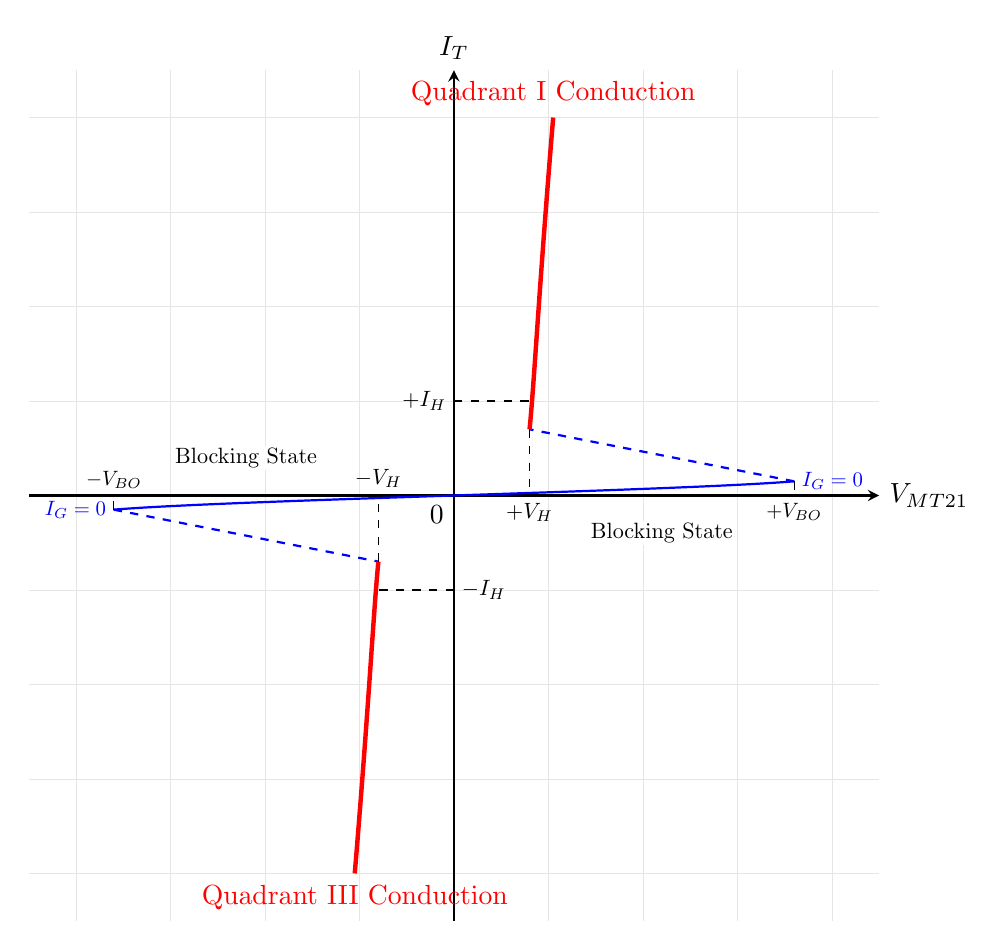
\begin{tikzpicture}[scale=1.2]
  % Grid
  \draw[very thin, gray!20] (-4.5,-4.5) grid (4.5,4.5);
  
  % Axes
  \draw[->, >=stealth, thick] (-4.5,0) -- (4.5,0) node[right] {$V_{MT21}$};
  \draw[->, >=stealth, thick] (0,-4.5) -- (0,4.5) node[above] {$I_T$};
  
  % Origin
  \node[below left] at (0,0) {$0$};

  % --- QUADRANT I: MT2 is POSITIVE ---
  % Forward Blocking (leakage)
  \draw[thick, blue] (0,0) .. controls (1.5,0.05) and (3.0,0.1) .. (3.6,0.15) node[right, scale=0.75] {$I_G = 0$};
  \draw[dashed, blue] (3.6,0.15) -- (0.8,0.7);
  \draw[dashed, thin, black] (3.6,0.15) -- (3.6,0) node[below, scale=0.75] {$+V_{BO}$};
  
  % Forward Conduction (ON-State)
  \draw[ultra thick, red] (0.8,0.7) .. controls (0.85,1.2) and (0.9,2.2) .. (1.05,4.0) node[above] {Quadrant I Conduction};
  \draw[dashed, thin] (0,1.0) node[left, scale=0.8] {$+I_H$} -- (0.85,1.0);
  \draw[dashed, thin] (0.8,0.7) -- (0.8,0) node[below, scale=0.8] {$+V_H$};

  % --- QUADRANT III: MT2 is NEGATIVE ---
  % Reverse Blocking (leakage)
  \draw[thick, blue] (0,0) .. controls (-1.5,-0.05) and (-3.0,-0.1) .. (-3.6,-0.15) node[left, scale=0.75] {$I_G = 0$};
  \draw[dashed, blue] (-3.6,-0.15) -- (-0.8,-0.7);
  \draw[dashed, thin, black] (-3.6,-0.15) -- (-3.6,0) node[above, scale=0.75] {$-V_{BO}$};
  
  % Reverse Conduction (ON-State)
  \draw[ultra thick, red] (-0.8,-0.7) .. controls (-0.85,-1.2) and (-0.9,-2.2) .. (-1.05,-4.0) node[below] {Quadrant III Conduction};
  \draw[dashed, thin] (0,-1.0) node[right, scale=0.8] {$-I_H$} -- (-0.85,-1.0);
  \draw[dashed, thin] (-0.8,-0.7) -- (-0.8,0) node[above, scale=0.8] {$-V_H$};

  % Labels for states
  \node[scale=0.8, fill=white, inner sep=1pt] at (2.2,-0.4) {Blocking State};
  \node[scale=0.8, fill=white, inner sep=1pt] at (-2.2,0.4) {Blocking State};
\end{tikzpicture}
\captionof{figure}{I-V Characteristics of a TRIAC}
\end{center}

\subsection*{2.3 Triggering Modes of a TRIAC}
Because both MT2 and the gate can be biased either positively or negatively with respect to MT1, a TRIAC can operate in four distinct triggering quadrants (modes), summarized below in order of standard gate sensitivity:

\begin{center}
\begin{tabular}{ccccc}
\toprule
\textbf{Mode} & \textbf{Quadrant} & \textbf{MT2 Voltage ($V_{MT21}$)} & \textbf{Gate Voltage ($V_{G1}$)} & \textbf{Gate Sensitivity} \\
\midrule
$\text{I}^{+}$ & I & Positive ($>0$) & Positive ($>0$) & \textbf{Highest} (Very easy to trigger) \\
$\text{III}^{-}$ & III & Negative ($<0$) & Negative ($<0$) & \textbf{High} (Very easy to trigger) \\
$\text{I}^{-}$ & I & Positive ($>0$) & Negative ($<0$) & \textbf{Medium} (Requires higher gate current) \\
$\text{III}^{+}$ & III & Negative ($<0$) & Positive ($>0$) & \textbf{Lowest} (Generally avoided in design) \\
\bottomrule
\end{tabular}
\captionof{table}{Triggering Modes and Sensitivities of a TRIAC}
\end{center}

\end{tcolorbox}

\item Explain the operating principle of a Silicon controlled Rectifier with the help of 'Two transistor model'.
\mk{20} \yr{EEE 263 | L-2/T-1 | 2011--12}

\begin{tcolorbox}[enhanced,breakable,ansbox,colback=cA!4,colframe=cA,boxrule=0.8pt,arc=5pt,title={\textbf{Answer}},fonttitle=\bfseries\color{white},colbacktitle=cA]

\section*{Two-Transistor Model of an SCR}

\subsection*{1. Introduction and Conceptual Splitting}
The operating principle of a Silicon Controlled Rectifier (SCR) can be modeled and analyzed using the **two-transistor analogy**. 
An SCR is a four-layer $P_1\text{-}N_1\text{-}P_2\text{-}N_2$ semiconductor device. By conceptually splitting the middle layers ($N_1$ and $P_2$) diagonally or horizontally, the structure can be viewed as two interconnected complementary transistors:
\begin{itemize}
    \item A \textbf{PNP transistor} ($Q_1$) formed by the layers $P_1\text{-}N_1\text{-}P_2$.
    \item An \textbf{NPN transistor} ($Q_2$) formed by the layers $N_1\text{-}P_2\text{-}N_2$.
\end{itemize}

\begin{center}
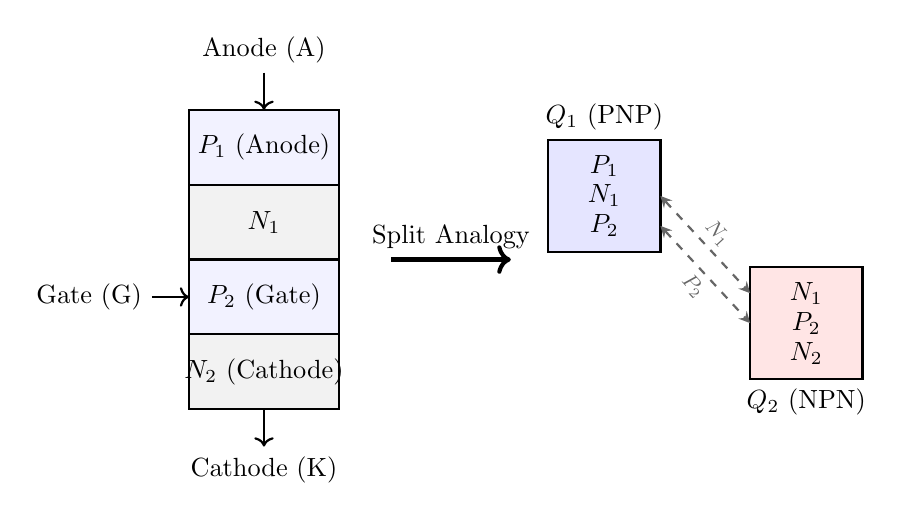
\begin{tikzpicture}[scale=0.95, every node/.style={transform shape}]
  % Left: 4-layer block
  \draw[thick, fill=blue!5] (0,3) rectangle (2,4) node[midway] {$P_1$ (Anode)};
  \draw[thick, fill=gray!10] (0,2) rectangle (2,3) node[midway] {$N_1$};
  \draw[thick, fill=blue!5] (0,1) rectangle (2,2) node[midway] {$P_2$ (Gate)};
  \draw[thick, fill=gray!10] (0,0) rectangle (2,1) node[midway] {$N_2$ (Cathode)};
  
  \draw[thick, ->] (1,4.5) -- (1,4) node[above, at start] {Anode (A)};
  \draw[thick, ->] (1,0) -- (1,-0.5) node[below, at end] {Cathode (K)};
  \draw[thick, ->] (-0.5,1.5) -- (0,1.5) node[left, at start] {Gate (G)};

  % Arrow pointing to equivalent split
  \draw[line width=1.5pt, ->] (2.7,2) -- (4.3,2) node[midway, above] {Split Analogy};

  % Right: PNP and NPN block split
  % PNP
  \draw[thick, fill=blue!10] (4.8,2.1) rectangle (6.3,3.6);
  \node at (5.55, 3.25) {$P_1$};
  \node at (5.55, 2.85) {$N_1$};
  \node at (5.55, 2.45) {$P_2$};
  \node[above] at (5.55, 3.6) {$Q_1$ (PNP)};
  
  % NPN
  \draw[thick, fill=red!10] (7.5,0.4) rectangle (9.0,1.9);
  \node at (8.25, 1.55) {$N_1$};
  \node at (8.25, 1.15) {$P_2$};
  \node at (8.25, 0.75) {$N_2$};
  \node[below] at (8.25, 0.4) {$Q_2$ (NPN)};

  % Interconnections between split layers
  \draw[thick, <->, >=stealth, dashed, gray!80!black] (6.3, 2.85) -- (7.5, 1.55) node[midway, above, sloped, scale=0.8] {$N_1$};
  \draw[thick, <->, >=stealth, dashed, gray!80!black] (6.3, 2.45) -- (7.5, 1.15) node[midway, below, sloped, scale=0.8] {$P_2$};
\end{tikzpicture}
\captionof{figure}{Conceptual splitting of the 4-layer SCR into PNP and NPN structures}
\end{center}

\subsection*{2. Equivalent Circuit Schematic}
In this interconnected model:
\begin{itemize}
    \item The Emitter of $Q_1$ is connected to the external \textbf{Anode (A)}.
    \item The Emitter of $Q_2$ is connected to the external \textbf{Cathode (K)}.
    \item The Base of $Q_1$ is tied to the Collector of $Q_2$ (forming the internal $N_1$ region).
    \item The Collector of $Q_1$ is tied to the Base of $Q_2$ and the external \textbf{Gate (G)} (forming the internal $P_2$ region).
\end{itemize}

\begin{center}
\begin{circuitikz}[scale=1.2]
  % PNP Transistor Q1
  \draw (0,1.8) node[pnp, scale=1.2] (Q1) {};
  \node[left=0.25cm] at (Q1.center) {$Q_1$};
  
  % NPN Transistor Q2
  \draw (2.2,0) node[npn, scale=1.2] (Q2) {};
  \node[right=0.25cm] at (Q2.center) {$Q_2$};

  % Connections
  \draw (Q1.C) |- (Q2.B);
  \draw (Q2.C) |- (Q1.B);

  % Terminals
  \draw (Q1.E) -- ++(0,0.5) node[above] {Anode (A)};
  \draw[->, >=stealth] ($(Q1.E)+(0,0.4)$) -- ($(Q1.E)+(0,0.15)$) node[midway, left] {$I_A$};

  \draw (Q2.E) -- ++(0,-0.5) node[below] {Cathode (K)};
  \draw[->, >=stealth] ($(Q2.E)+(0,-0.15)$) -- ($(Q2.E)+(0,-0.4)$) node[midway, right] {$I_K$};

  % Gate node
  \draw (Q2.B) -- ++(-0.6, 0) node[circle, fill, inner sep=1.5pt] (gnode) {} -- ++(-0.6,0) node[left] {Gate (G)};
  \draw[->, >=stealth] ($(gnode)+(-0.4, 0.2)$) -- ($(gnode)+(-0.1, 0.2)$) node[midway, above] {$I_G$};
  \draw (Q1.C) |- (gnode);

  % Currents
  \node[right, scale=0.9] at ($(Q1.C)+(0,-0.2)$) {$I_{C1}$};
  \node[right, scale=0.9] at ($(Q2.C)+(0,0.2)$) {$I_{C2}$};
  \node[above, scale=0.9] at ($(Q1.B)+(-0.3,0)$) {$I_{B1}$};
  \node[above, scale=0.9] at ($(Q2.B)+(-0.3,0)$) {$I_{B2}$};
\end{circuitikz}
\captionof{figure}{Two-Transistor Equivalent Schematic of an SCR}
\end{center}

\subsection*{3. Mathematical Derivation of Anode Current}
Let us define the parameters for both transistors:
\begin{itemize}
    \item $\alpha_1, \alpha_2$: Common-base current gains of $Q_1$ and $Q_2$, respectively.
    \item $I_{CO1}, I_{CO2}$: Reverse collector-to-base leakage currents of $Q_1$ and $Q_2$.
\end{itemize}

For $Q_1$ (PNP), the collector current $I_{C1}$ is expressed as:
\begin{equation}
I_{C1} = \alpha_1 I_{E1} + I_{CO1}
\end{equation}
Since the emitter of $Q_1$ is connected directly to the anode, $I_{E1} = I_A$:
\begin{equation}
I_{C1} = \alpha_1 I_A + I_{CO1} \label{eq:IC1}
\end{equation}

Similarly, for $Q_2$ (NPN), the collector current $I_{C2}$ is:
\begin{equation}
I_{C2} = \alpha_2 I_{E2} + I_{CO2}
\end{equation}
Since the emitter of $Q_2$ is connected to the cathode, $I_{E2} = I_K$:
\begin{equation}
I_{C2} = \alpha_2 I_K + I_{CO2} \label{eq:IC2}
\end{equation}

From Kirchhoff's Current Law (KCL) applied to the combined system, the total current entering the anode must exit through the base-collector junctions:
\begin{equation}
I_A = I_{C1} + I_{C2} \label{eq:KCL_IA}
\end{equation}
Furthermore, the cathode current $I_K$ is the sum of the anode current and the gate current:
\begin{equation}
I_K = I_A + I_G \label{eq:IK}
\end{equation}

Substituting Equations \eqref{eq:IC1}, \eqref{eq:IC2}, and \eqref{eq:IK} into Equation \eqref{eq:KCL_IA}:
\begin{align*}
I_A &= \left(\alpha_1 I_A + I_{CO1}\right) + \left(\alpha_2 (I_A + I_G) + I_{CO2}\right) \\
I_A &= (\alpha_1 + \alpha_2)I_A + \alpha_2 I_G + (I_{CO1} + I_{CO2})
\end{align*}

Grouping the $I_A$ terms together:
\begin{equation}
I_A \left[1 - (\alpha_1 + \alpha_2)\right] = \alpha_2 I_G + I_{CO}
\end{equation}
where $I_{CO} = I_{CO1} + I_{CO2}$ is the total reverse saturation leakage current of the central blocking junction.

Solving for the anode current $I_A$:
\begin{equation}
I_A = \frac{\alpha_2 I_G + I_{CO}}{1 - (\alpha_1 + \alpha_2)} \label{eq:final_SCR}
\end{equation}

\subsection*{4. Analysis of SCR Operation States}

Using the derived relationship in Equation \eqref{eq:final_SCR}, we can analyze the two primary states of the SCR:

\subsubsection*{A. OFF-State (Forward Blocking)}
When the gate current is zero ($I_G = 0$):
\begin{equation}
I_A = \frac{I_{CO}}{1 - (\alpha_1 + \alpha_2)}
\end{equation}
For silicon transistors operating at low currents, the current gains $\alpha_1$ and $\alpha_2$ are extremely small ($\alpha \ll 1$). Consequently:
\begin{equation}
(\alpha_1 + \alpha_2) \ll 1 \implies I_A \approx I_{CO}
\end{equation}
In this condition, only a tiny reverse saturation leakage current flows, and the SCR remains in its high-impedance OFF (forward blocking) state.

\subsubsection*{B. Regenerative Turn-on Process (ON-State)}
When a positive trigger current $I_G$ is injected into the gate:
\begin{enumerate}
    \item $I_G$ acts as the base current $I_{B2}$ of $Q_2$, causing an increase in collector current $I_{C2}$.
    \item Since the collector of $Q_2$ is tied to the base of $Q_1$, $I_{C2}$ increases $I_{B1}$, turning $Q_1$ ON.
    \item Turning $Q_1$ ON increases $I_{C1}$.
    \item Because the collector of $Q_1$ is connected back to the base of $Q_2$, $I_{C1}$ flows into the base of $Q_2$, further increasing $I_{B2}$ even if the external gate signal $I_G$ is removed.
\end{enumerate}

This forms a closed \textbf{positive feedback loop} (regenerative action). As internal currents rise rapidly, the common-base current gains $\alpha_1$ and $\alpha_2$ of both silicon transistors increase toward their maximum values.
As the sum of the gains approaches unity:
\begin{equation}
(\alpha_1 + \alpha_2) \to 1 \implies \left[1 - (\alpha_1 + \alpha_2)\right] \to 0
\end{equation}
According to Equation \eqref{eq:final_SCR}, the denominator approaches zero, causing the anode current $I_A$ to surge abruptly. The device enters its low-impedance ON (forward conduction) state, limited only by the external load resistance. Once latched, the gate loses control, and the SCR remains ON.

\subsubsection*{C. Turn-off (Commutation)}
To turn the SCR OFF, the external anode current $I_A$ must be reduced below the characteristic \textbf{holding current} ($I_H$). This drop in current reduces the internal emitter currents, causing $\alpha_1$ and $\alpha_2$ to decrease. Once $(\alpha_1 + \alpha_2) < 1$, the regenerative feedback loop can no longer sustain itself, and the SCR transitions back to its blocking state.

\end{tcolorbox}



\end{enumerate}


%%──────────────────────────────────────────────────────────────────────
\subtopic{cB}{Miscellaneous}
\label{sub:s1-Miscellaneous}

\begin{enumerate}
    
\item Why is digital processing of data advantageous over analog processing?
\mk{6} \yr{EEE 263 | L-2/T-1 | 2013--14}

\begin{tcolorbox}[enhanced,breakable,ansbox,colback=cA!4,colframe=cA,boxrule=0.8pt,arc=5pt,title={\textbf{Answer}},fonttitle=\bfseries\color{white},colbacktitle=cA]

\subsection*{Advantages of Digital Processing over Analog Processing}

While the real physical world is inherently analog (continuous in time and amplitude), processing data digitally (discrete in time and amplitude) has become the dominant paradigm in modern electronics. The fundamental advantage of digital processing stems from representing information as discrete binary states (0s and 1s) rather than continuous voltage or current levels. 

The primary advantages of digital processing over analog processing are detailed below:

\begin{enumerate}
    \item \textbf{Superior Noise Immunity and Signal Regeneration:}
    \begin{itemize}
        \item \textit{Principle:} In an analog system, any added electrical noise becomes an inseparable part of the signal, degrading the signal-to-noise ratio (SNR) permanently. In a digital system, signals are represented by voltage ranges (e.g., $0$ to $0.8\,\text{V}$ for Logic 0, and $2.0$ to $5.0\,\text{V}$ for Logic 1). 
        \item \textit{Advantage:} As long as the noise amplitude does not exceed the defined \textit{noise margins}, the original discrete logic level can be perfectly regenerated and completely stripped of noise at each processing stage.
    \end{itemize}

    \item \textbf{Reproducibility and Stability:}
    \begin{itemize}
        \item \textit{Principle:} Analog circuits are highly sensitive to component tolerances, temperature variations, power supply fluctuations, and component aging. 
        \item \textit{Advantage:} Digital circuits operate on logic thresholds. A digital calculation will yield the exact same result every time, independent of minor temperature drifts or component aging, ensuring absolute reproducibility across millions of manufactured devices.
    \end{itemize}

    \item \textbf{Programmability and Flexibility:}
    \begin{itemize}
        \item \textit{Principle:} Analog signal processing requires dedicated hardware (specific resistor, capacitor, and op-amp configurations) to perform a specific function (e.g., filtering). 
        \item \textit{Advantage:} Digital Signal Processing (DSP) is primarily software-driven. The same physical microprocessor or DSP chip can be reprogrammed to act as a low-pass filter, a high-pass filter, or a complex audio equalizer simply by updating its code, without altering the physical circuitry.
    \end{itemize}

    \item \textbf{Error Detection and Correction:}
    \begin{itemize}
        \item \textit{Principle:} Analog signals have no inherent way to verify their own integrity.
        \item \textit{Advantage:} Digital data can be supplemented with redundant information (e.g., parity bits, Cyclic Redundancy Checks (CRC), and Hamming codes). This allows digital systems to autonomously detect and mathematically correct data corruption that occurs during transmission or storage.
    \end{itemize}

    \item \textbf{Data Storage and Retrieval:}
    \begin{itemize}
        \item \textit{Principle:} Analog storage media (like magnetic tape or vinyl) degrade slightly with every read/write cycle and over time.
        \item \textit{Advantage:} Digital data can be stored in solid-state drives, RAM, or optical media with zero degradation over time. Data can be copied and retrieved an infinite number of times with 100\% perfect fidelity.
    \end{itemize}

    \item \textbf{Ease of Multiplexing and Transmission:}
    \begin{itemize}
        \item \textit{Advantage:} Digital signals are highly amenable to Time-Division Multiplexing (TDM) and packet-switching networks (like the Internet). Furthermore, digital data can be easily compressed (to save bandwidth) and heavily encrypted (using cryptographic algorithms) for secure transmission, which is extraordinarily difficult and less effective in the analog domain.
    \end{itemize}

    \item \textbf{Miniaturization and Cost (VLSI/ULSI Integration):}
    \begin{itemize}
        \item \textit{Advantage:} Digital circuits, primarily consisting of simple switching transistors (like CMOS), scale down incredibly well. Modern fabrication technologies allow billions of identical digital transistors to be packed onto a single silicon chip at a microscopic scale, drastically reducing the cost, power consumption, and physical footprint per computational operation compared to equivalent analog networks.
    \end{itemize}
\end{enumerate}

\subsection*{Summary}
Analog processing is generally restricted to the very front-end (sensors, ADCs) and back-end (DACs, actuators) of modern systems to interface with the physical world. The core processing, however, is executed digitally due to its unmatched robustness, flexibility, scalability, and exact reproducibility.

\end{tcolorbox}

\item Why do we need to miniaturize a transistor as much as possible? If you continue to miniaturize the transistor (switch), what problems may surface?
\mk{5} \yr{EEE 263 | L-2/T-1 | 2013--14}

\begin{tcolorbox}[enhanced,breakable,ansbox,colback=cA!4,colframe=cA,boxrule=0.8pt,arc=5pt,title={\textbf{Answer}},fonttitle=\bfseries\color{white},colbacktitle=cA]

\subsection*{1. The Need for Transistor Miniaturization (Scaling)}

The continuous reduction in the physical dimensions of transistors, primarily driven by Moore's Law, is motivated by several fundamental advantages in digital and analog circuit design. The primary reasons for miniaturization include:

\begin{itemize}
    \item \textbf{Increased Device Density (Functionality):} Smaller transistors allow for a higher number of devices to be packed onto a single silicon die. This enables the integration of more complex architectures, more memory (cache), and multi-core processors on a single chip, drastically increasing computational power.
    \item \textbf{Higher Switching Speed (Performance):} The transit time ($t_r$) for charge carriers (electrons or holes) to cross the channel from source to drain is directly proportional to the square of the channel length ($L$) in the low-field regime:
    \begin{equation}
        t_r \approx \frac{L^2}{\mu V_{DS}}
    \end{equation}
    Reducing $L$ decreases the transit time, inherently increasing the maximum operating frequency ($f_T$) of the transistor. Furthermore, smaller devices have lower parasitic capacitances, which allows them to charge and discharge faster.
    \item \textbf{Reduced Dynamic Power Consumption:} Dynamic power dissipation in CMOS circuits is given by:
    \begin{equation}
        P_{dynamic} = \alpha \cdot f \cdot C_{load} \cdot V_{DD}^2
    \end{equation}
    Miniaturization reduces the physical area, which decreases the gate and parasitic node capacitances ($C_{load}$). Historically, scaling rules (like Dennard Scaling) also dictated a reduction in the supply voltage ($V_{DD}$), leading to a quadratic reduction in dynamic power per gate.
    \item \textbf{Lower Cost per Transistor:} By making transistors smaller, more integrated circuits (dies) can be fabricated on a single silicon wafer. Since the cost of processing a wafer is relatively constant, the cost per chip—and therefore the cost per transistor—decreases significantly.
\end{itemize}

\rule{\textwidth}{0.4pt}

\subsection*{2. Problems and Challenges of Continuous Miniaturization}

While scaling down provides immense benefits, pushing the dimensions into the deep-submicron and nanometer regimes introduces severe physical and electrical limitations. The major problems that surface include:

\begin{itemize}
    \item \textbf{Short-Channel Effects (SCE):}
    As the channel length $L$ becomes comparable to the depletion widths of the source and drain junctions, the gate loses its dominant control over the channel potential. The source and drain electric fields begin to interfere with the gate's ability to turn the transistor off completely.
    
    \item \textbf{Drain-Induced Barrier Lowering (DIBL):}
    A specific short-channel effect where a high drain voltage ($V_{DS}$) lowers the potential barrier between the source and the channel. This allows electrons to flow from source to drain even when the gate voltage is below the threshold voltage, effectively reducing the effective threshold voltage ($V_{th}$) and increasing leakage.
    
    \item \textbf{Subthreshold Leakage Current:}
    To maintain performance at lower supply voltages, the threshold voltage ($V_{th}$) must also be scaled down. However, subthreshold current follows an exponential relationship:
    \begin{equation}
        I_{sub} \propto \exp\left( \frac{V_{GS} - V_{th}}{n V_T} \right)
    \end{equation}
    Lowering $V_{th}$ results in an exponential increase in leakage current when the transistor is in the OFF state, leading to massive static power dissipation.
    
    \item \textbf{Gate Oxide Tunneling (Leakage):}
    To maintain gate control over a shorter channel, the gate oxide thickness ($t_{ox}$) must be scaled down proportionally. When $SiO_2$ thickness falls below $2\,\text{nm}$ (only a few atomic layers thick), charge carriers can pass through the dielectric via \textit{Quantum Mechanical Tunneling}, creating a severe gate leakage current. (This necessitated the transition to High-k dielectrics and metal gates).
    
    \item \textbf{Velocity Saturation and Mobility Degradation:}
    In very short channels, the longitudinal electric field ($E = V_{DS}/L$) becomes extremely high. Carriers reach their maximum drift velocity (velocity saturation) earlier, meaning current does not increase quadratically with gate voltage anymore, but rather linearly. High vertical electric fields also pull carriers toward the Si-$SiO_2$ interface, causing surface scattering and reducing carrier mobility ($\mu$).
    
    \item \textbf{Thermal and Power Density Issues (Dark Silicon):}
    Although power per transistor decreases, the number of transistors per unit area increases at a faster rate. This leads to an overall increase in power density ($\text{W/cm}^2$). Dissipating this heat becomes physically impossible with standard cooling, forcing parts of the chip to be powered down during operation (a phenomenon known as "Dark Silicon").
    
    \item \textbf{Process Variations and Random Dopant Fluctuations (RDF):}
    At the nanometer scale, exact manufacturing becomes impossible. A variation of just a few atoms in the channel region can drastically alter the threshold voltage. Random placement of dopant atoms (RDF) and edge roughness cause huge variations in performance between adjacent transistors on the same chip.
    
    \item \textbf{Interconnect RC Delay:}
    As transistors shrink and speed up, the metal wires connecting them must also become thinner and closer together. This increases both wire resistance ($R$) and inter-wire parasitic capacitance ($C$). In modern nodes, the $RC$ delay of the interconnects limits the overall speed of the chip more than the intrinsic delay of the transistors themselves.
\end{itemize}

\end{tcolorbox}

\item Write a script in C language that takes a sinusoidal input and provides a full-wave rectified output.
\mk{5} \yr{EEE 263 | L-2/T-1 | 2013--14}

\begin{tcolorbox}[enhanced,breakable,ansbox,colback=cA!4,colframe=cA,boxrule=0.8pt,arc=5pt,title={\textbf{Answer}},fonttitle=\bfseries\color{white},colbacktitle=cA]

\subsection*{1. Mathematical Modeling of a Full-Wave Rectifier}
In electronic circuits, an ideal full-wave rectifier converts the entire input waveform to one of constant polarity at its output. If the input is a continuous sinusoidal signal, the mathematical representation is simply the absolute value of the input.

Let the input sinusoidal voltage be:
\begin{equation}
    v_{in}(t) = V_p \sin(2 \pi f t)
\end{equation}
where $V_p$ is the peak amplitude and $f$ is the frequency of the signal.

The ideal full-wave rectified output is:
\begin{equation}
    v_{out}(t) = |v_{in}(t)| = |V_p \sin(2 \pi f t)|
\end{equation}

For a practical implementation, a bridge rectifier experiences a voltage drop across two forward-biased diodes (approximately $2V_D$). A practical software model could include this threshold, but for general digital signal processing or simulation of the rectification concept, the absolute value function $\left(\texttt{fabs()}\text{ in C}\right)$ is sufficient.

\begin{center}
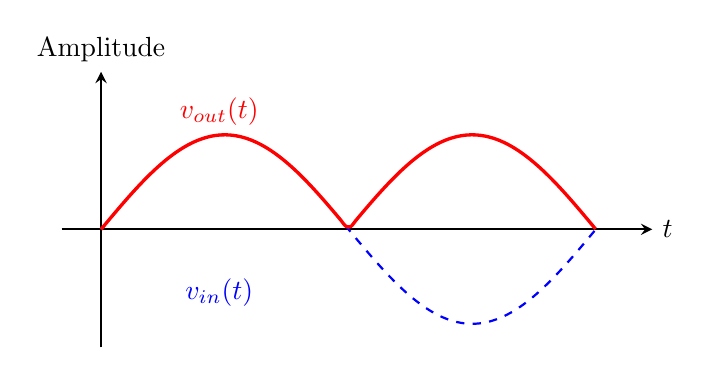
\begin{tikzpicture}[scale=1, thick]
    % Axes
    \draw[->, >=stealth] (-0.5,0) -- (7,0) node[right] {$t$};
    \draw[->, >=stealth] (0,-1.5) -- (0,2) node[above] {Amplitude};
    
    % Input Sine Wave
    \draw[domain=0:6.28, samples=100, smooth, variable=\x, blue, dashed] plot ({\x}, {1.2*sin(\x*180/3.14159)});
    
    % Output Full-Wave Rectified Wave
    \draw[domain=0:6.28, samples=100, smooth, variable=\x, red, very thick] plot ({\x}, {abs(1.2*sin(\x*180/3.14159))});
    
    % Labels
    \node[blue] at (1.5, -0.8) {$v_{in}(t)$};
    \node[red] at (1.5, 1.5) {$v_{out}(t)$};
\end{tikzpicture}
\end{center}

\rule{\textwidth}{0.4pt}

\subsection*{2. C Language Implementation}
The following C script generates discrete time steps, computes the corresponding sinusoidal input values, applies full-wave rectification using the \texttt{math.h} library's absolute value function, and prints the tabulated results.

\begin{verbatim}
#include <stdio.h>
#include <math.h>

#define PI 3.14159265358979323846
#define FREQUENCY 50.0        // Signal frequency in Hz
#define AMPLITUDE 10.0        // Peak voltage in Volts
#define SAMPLING_RATE 1000.0 // Samples per second
#define NUM_SAMPLES 40        // Total number of samples to generate

int main() {
    double t;      // Time variable
    double v_in;   // Input voltage
    double v_out;  // Rectified output voltage

    // Print table header
    printf("Time (ms) \t V_in (V) \t V_out (V)\n");
    printf("------------------------------------------\n");

    // Generate and process the signal
    for (int i = 0; i <= NUM_SAMPLES; i++) {
        // Calculate current time step in seconds
        t = i / SAMPLING_RATE;
        
        // Generate sinusoidal input
        v_in = AMPLITUDE * sin(2.0 * PI * FREQUENCY * t);
        
        // Perform ideal full-wave rectification
        v_out = fabs(v_in);
        
        // Print results (Time converted to ms for readability)
        printf("%8.1f \t %8.4f \t %8.4f\n", t * 1000.0, v_in, v_out);
    }

    return 0;
}
\end{verbatim}

\subsection*{3. Code Explanation}
\begin{itemize}
    \item \textbf{Constants:} The signal frequency is defined as $50\,\text{Hz}$ with a peak amplitude of $10\,\text{V}$. The sampling rate dictates the time resolution of our discrete signal.
    \item \textbf{Loop Execution:} The \texttt{for} loop iterates through each sample index \texttt{i}, mapping it to a continuous time equivalent $t = i / f_s$.
    \item \textbf{Signal Generation:} The function \texttt{sin()} calculates the instantaneous amplitude of the input sine wave at time $t$.
    \item \textbf{Rectification:} The \texttt{fabs()} (float absolute) function strips the negative sign from the input, effectively folding the negative half-cycles of the sine wave into the positive domain, mirroring the action of a diode bridge.
\end{itemize}

\end{tcolorbox}

\item How does a computer program rectify the sinusoidal input mentioned above? Is there any diode inside the processor? If not, what makes that act of rectification possible?
\mk{10} \yr{EEE 263 | L-2/T-1 | 2013--14}

\begin{tcolorbox}[enhanced,breakable,ansbox,colback=cA!4,colframe=cA,boxrule=0.8pt,arc=5pt,title={\textbf{Answer}},fonttitle=\bfseries\color{white},colbacktitle=cA]

\subsection*{1. Digital Rectification vs. Analog Rectification}
In traditional analog electronics, rectification of a sinusoidal signal is achieved using semiconductor diodes, which physically block the flow of reverse current due to their non-linear $I$-$V$ characteristics. However, a \textbf{computer program} does not operate on continuous physical voltages; it operates on discrete numerical data. 

To process an analog sinusoidal signal in a computer, the signal must first be sampled and quantized by an \textbf{Analog-to-Digital Converter (ADC)}. The ADC converts the continuous voltage waveform, $v(t)$, into a discrete-time sequence of binary numbers, $x[n]$. The act of "rectification" is then performed purely through \textbf{mathematical operations} on these numbers.

\subsection*{2. Are there Diodes Inside the Processor?}
\textbf{No, physical diodes are not used to perform rectification inside a processor.} 
While a modern microprocessor contains billions of transistors (MOSFETs) which inherently possess parasitic body diodes, these diodes are never used for analog signal processing. The processor is entirely composed of digital logic gates (AND, OR, NOT, etc.) forming structural blocks like the \textbf{Arithmetic Logic Unit (ALU)}. The processor treats the sinusoidal signal merely as a stream of binary numbers (often in two's complement format).

\subsection*{3. What Makes Software Rectification Possible?}
The rectification is made possible by the \textbf{Arithmetic Logic Unit (ALU)} executing specific logical and mathematical instructions defined by the computer program. Since the sinusoidal signal is represented numerically, where negative voltages are typically represented as negative integers (via the sign bit), rectification is reduced to simple conditional logic or arithmetic:

\begin{itemize}
    \item \textbf{Half-Wave Rectification:} The program inspects the sign bit of each data sample $x[n]$. If the sample is negative, it is overwritten with zero. If it is positive, it is kept unchanged.
    \begin{equation}
        y[n] = 
        \begin{cases} 
            x[n], & \text{if } x[n] \geq 0 \\
            0, & \text{if } x[n] < 0 
        \end{cases}
    \end{equation}
    
    \item \textbf{Full-Wave Rectification:} The program computes the absolute value of the incoming data sample. At the machine level, if the sign bit indicates a negative number, the ALU takes the two's complement (inverts all bits and adds 1) to make it positive.
    \begin{equation}
        y[n] = |x[n]| = 
        \begin{cases} 
            x[n], & \text{if } x[n] \geq 0 \\
            -x[n], & \text{if } x[n] < 0 
        \end{cases}
    \end{equation}
\end{itemize}

\subsection*{4. Block Diagram of Digital Rectification}
The following system block diagram illustrates how a physical continuous sine wave is mathematically rectified without the use of physical diodes.

\begin{center}
    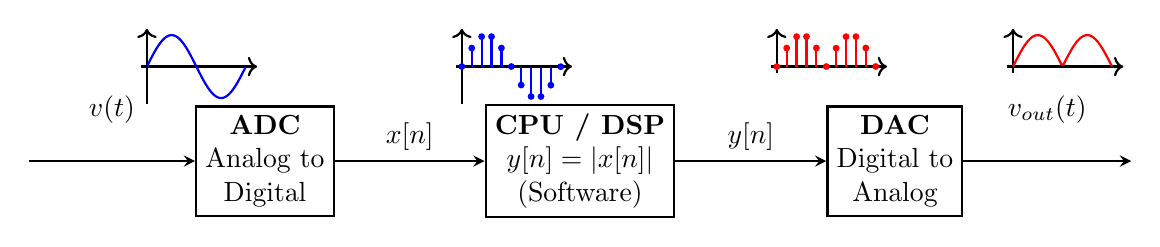
\begin{tikzpicture}[thick,scale=1.0, every node/.style={transform shape}]
        
        % Block definitions
        \tikzstyle{block} = [draw, rectangle, minimum height=3em, minimum width=4em, align=center, fill=white]
        
        % Blocks
        \node[block] (adc) at (0,0) {\textbf{ADC} \\ Analog to \\ Digital};
        \node[block] (cpu) at (4,0) {\textbf{CPU / DSP} \\ $y[n] = |x[n]|$ \\ (Software)};
        \node[block] (dac) at (8,0) {\textbf{DAC} \\ Digital to \\ Analog};
        
        % Inputs and Outputs
        \coordinate (input) at (-3,0);
        \coordinate (output) at (11,0);
        
        % Arrows
        \draw[->, >=stealth] (input) -- (adc) node[midway, above=10pt] {$v(t)$};
        \draw[->, >=stealth] (adc) -- (cpu) node[midway, above] {$x[n]$};
        \draw[->, >=stealth] (cpu) -- (dac) node[midway, above] {$y[n]$};
        \draw[->, >=stealth] (dac) -- (output) node[midway, above=10pt] {$v_{out}(t)$};
        
        % Mini Waveform 1: Analog Sine
        \begin{scope}[shift={(-1.5, 1.2)}, scale=0.4]
            \draw[->] (-0.2,0) -- (3.5,0);
            \draw[->] (0,-1.2) -- (0,1.2);
            \draw[blue, thick, domain=0:3.14, samples=50] plot (\x, {sin(\x r * 2)});
        \end{scope}

        % Mini Waveform 2: Discrete Sine
        \begin{scope}[shift={(2.5, 1.2)}, scale=0.4]
            \draw[->] (-0.2,0) -- (3.5,0);
            \draw[->] (0,-1.2) -- (0,1.2);
            \foreach \x in {0,0.314,...,3.14} {
                \draw[blue, fill=blue] (\x, {sin(\x r * 2)}) circle (2pt);
                \draw[blue] (\x, 0) -- (\x, {sin(\x r * 2)});
            }
        \end{scope}

        % Mini Waveform 3: Discrete Rectified
        \begin{scope}[shift={(6.5, 1.2)}, scale=0.4]
            \draw[->] (-0.2,0) -- (3.5,0);
            \draw[->] (0,-0.2) -- (0,1.2);
            \foreach \x in {0,0.314,...,3.14} {
                \draw[red, fill=red] (\x, {abs(sin(\x r * 2))}) circle (2pt);
                \draw[red] (\x, 0) -- (\x, {abs(sin(\x r * 2))});
            }
        \end{scope}
        
        % Mini Waveform 4: Analog Rectified
        \begin{scope}[shift={(9.5, 1.2)}, scale=0.4]
            \draw[->] (-0.2,0) -- (3.5,0);
            \draw[->] (0,-0.2) -- (0,1.2);
            \draw[red, thick, domain=0:3.14, samples=50] plot (\x, {abs(sin(\x r * 2))});
        \end{scope}
        
    \end{tikzpicture}
\end{center}

\subsection*{Summary}
In a digital system, the act of \textbf{rectification is abstracted from physics to mathematics}. The physical non-linear characteristics of a PN junction (diode) are replaced by the logical branching and arithmetic capability of the microprocessor's ALU processing discrete digital samples.

\end{tcolorbox}

\end{enumerate}



%% ══════════════════════════════════════════════════════════════════════
%%  PART II
%% ══════════════════════════════════════════════════════════════════════
\secdivider{S2 --- Clipping, clamping circuits}{Clipping, clamping circuits using diodes }{cA}

%% ══════════════════════════════════════════════════════════════════════
%%  SECTION 4: CLIPPING, CLAMPING & SWITCHING
%% ══════════════════════════════════════════════════════════════════════
\markboth{S2: Clipping, Clamping circuits}{S4: Clipping, Clamping circuits}
\label{sec:S2}
\titleformat{\section}{\large\bfseries\color{cA}}{}{0em}{}[\titlerule]
\section*{S2 \quad Clipping, Clamping Circuits}
\addcontentsline{toc}{section}{S2: Clipping, Clamping Circuits}


%%──────────────────────────────────────────────────────────────────────
\subtopic{cA}{Clipping Circuits --- Waveform \& Transfer Characteristics}
\label{sub:s2-clipping}

\begin{enumerate}
    
\item For the circuit given, plot $v_0$ vs time. The input $v_1$ is a sine wave with 5\,V amplitude and 1\,kHz frequency. Assume 0.7\,V voltage drop across diodes in forward bias.
\begin{center}
    
    \begin{circuitikz}[thick]
        
        % --- Input Voltage Source and Top Resistor ---
        % V_I with positive terminal up
        \draw (0, 4) to[V, l=$V_I$] (0, 0) ;
                     \draw ( 0,4) to[R, l=$5\text{ k}\Omega$] (3, 4);
        
        % --- Middle Branch ---
        % Drawn top-to-bottom. 
        % 'l' places label on the right, 'l_' places it on the left.
        \draw (3, 4) to[R, l=$10\text{ k}\Omega$] (3, 2.5)
                     to[D, l_=$D_1$] (3, 1.2)
                     to[battery1, l=$1\text{ V}$] (3, 0);
                     
        % --- Top and Bottom Wire Connections ---
        \draw (3, 4) -- (6, 4);
        \draw (0, 0) -- (6, 0);
        
        % --- Right Branch ---
        \draw (6, 4) to[R, l=$5\text{ k}\Omega$] (6, 2.5);
                    \draw ( 6,1.2) to[D, l=$D_2$] (6, 2.5);
                    \draw ( 6, 0) to[battery1, l=$2\text{ V}$] (6, 1.2);
                     
        % --- Junction Nodes (Dots) ---
        \node[circ] at (3, 4) {};
        \node[circ] at (3, 0) {};
        \node[circ] at (6, 4) {};
        \node[circ] at (6, 0) {};
                     
        % --- Output Terminals ---
        \draw (6, 4) -- (7.5, 4) node[ocirc] {};
        \draw (6, 0) -- (7.5, 0) node[ocirc] {};
        
        % Output Voltage Labels (+, v_o, -)
        \node at (8.2, 4) {$+$};
        \node at (8.2, 2) {$v_o$};
        \node at (8.2, 0) {$-$};

    \end{circuitikz}
\end{center}
\mk{14} \yr{EEE 263 | L-2/T-1 | 2022--23}

\begin{tcolorbox}[enhanced,breakable,ansbox,colback=cA!4,colframe=cA,boxrule=0.8pt,arc=5pt,title={\textbf{Answer}},fonttitle=\bfseries\color{white},colbacktitle=cA]

\subsection*{1. Circuit Theory and Assumptions}
The given circuit is a parallel diode clipper (or limiter) that shapes the input waveform by limiting its voltage excursions in both the positive and negative directions. 
\begin{itemize}
    \item \textbf{Input Signal:} $v_I(t) = 5\sin(2\pi \cdot 1000 t)$ V. 
    \item \textbf{Diode Model:} We assume the Constant Voltage Drop (CVD) model, where a forward-biased diode acts as a $V_\gamma = 0.7$ V voltage source, and a reverse-biased diode acts as an open circuit.
\end{itemize}

\begin{center}
    \begin{circuitikz}[thick, american, scale=0.9, transform shape]
        % Input
        \draw (0,0) to[sV, v=$v_I(t)$] (0,4);
        % Series R
        \draw (0,4) to[R, l=$5\text{ k}\Omega$, i=$i_{in}$] (4,4);
        
        % Branch 1 (D1)
        \draw (4,4) node[circ]{} node[above]{$v_o$} 
              to[R, l=$10\text{ k}\Omega$, i=$i_{D1}$] (4,2.5);
        \draw (4,2.5) to[D, l=$D_1$] (4,1.2);
        \draw (4,0) node[circ]{} to[battery1,invert,  l=$1\text{ V}$] (4,1.2);
        
        % Branch 2 (D2)
        \draw (7,4) node[circ]{} to[R, l=$5\text{ k}\Omega$, i<=$i_{D2}$] (7,2.5);
        \draw (7,1.2) to[D, l=$D_2$] (7,2.5); % Diode D2 points up
        \draw (7,0) node[circ]{} to[battery1, l=$2\text{ V}$] (7,1.2);
        
        % Rails
        \draw (4,4) -- (9,4);
        \draw (0,0) -- (9,0);
        
        % Output Terminals
        \draw (9,4) node[ocirc]{};
        \draw (9,0) node[ocirc]{} node[ground]{};
        
        \node at (9.4, 4) {$+$};
        \node at (9.4, 2) {$v_o(t)$};
        \node at (9.4, 0) {$-$};
    \end{circuitikz}
\end{center}

\subsection*{2. Determination of Operating Regions}
To plot the output waveform $v_o(t)$, we must determine the critical transition voltages where the diodes change states. Let the potential at the output node be $v_o$.

\subsubsection*{Condition for $D_1$ to turn ON:}
Diode $D_1$ points downwards. For it to conduct, the potential at $v_o$ must overcome the $1\text{ V}$ DC source and the $0.7\text{ V}$ diode drop. 
\begin{align*}
    v_o > 1\text{ V} + 0.7\text{ V} \implies v_o > 1.7\text{ V}
\end{align*}

\subsubsection*{Condition for $D_2$ to turn ON:}
Diode $D_2$ points upwards. For it to conduct, the $2\text{ V}$ DC source must be capable of pushing current up through $D_2$ to node $v_o$. The voltage drop from the source to $v_o$ must overcome the $0.7\text{ V}$ diode drop.
\begin{align*}
    2\text{ V} - v_o > 0.7\text{ V} \implies v_o < 1.3\text{ V}
\end{align*}

This defines three distinct operating regions based on the input voltage $v_I$. Note that $v_o$ can never be simultaneously $> 1.7\text{ V}$ and $< 1.3\text{ V}$, hence $D_1$ and $D_2$ are never ON at the same time.

---

\subsection*{3. Mathematical Derivation of Transfer Characteristics}

\textbf{Region I: Both $D_1$ and $D_2$ OFF ($1.3\text{ V} \le v_I \le 1.7\text{ V}$)} \\
When both diodes are OFF, they act as open circuits. No current flows through the $5\text{ k}\Omega$ series resistor. 
\begin{equation}
    v_o = v_I
\end{equation}

\textbf{Region II: $D_1$ ON, $D_2$ OFF ($v_I > 1.7\text{ V}$)} \\
$D_1$ acts as a $0.7\text{ V}$ source. The $D_1$ branch can be modeled as a $1.7\text{ V}$ equivalent source in series with the $10\text{ k}\Omega$ resistor. Applying Kirchhoff's Current Law (KCL) at node $v_o$:
\begin{align*}
    \frac{v_o - v_I}{5} + \frac{v_o - 1.7}{10} &= 0 \\
    2(v_o - v_I) + (v_o - 1.7) &= 0 \\
    3v_o &= 2v_I + 1.7 \\
    v_o &= \frac{2}{3}v_I + 0.567\text{ V}
\end{align*}
\textit{Peak Positive Voltage:} When $v_I = 5\text{ V}$, $v_o = \frac{2(5) + 1.7}{3} = 3.9\text{ V}$.

\vspace{0.5cm}

\textbf{Region III: $D_1$ OFF, $D_2$ ON ($v_I < 1.3\text{ V}$)} \\
$D_2$ acts as a $0.7\text{ V}$ source (opposing the $2\text{ V}$ source). The $D_2$ branch can be modeled as a $(2 - 0.7) = 1.3\text{ V}$ equivalent source in series with the $5\text{ k}\Omega$ resistor. Applying KCL at node $v_o$:
\begin{align*}
    \frac{v_o - v_I}{5} + \frac{v_o - 1.3}{5} &= 0 \\
    (v_o - v_I) + (v_o - 1.3) &= 0 \\
    2v_o &= v_I + 1.3 \\
    v_o &= 0.5v_I + 0.65\text{ V}
\end{align*}
\textit{Peak Negative Voltage:} When $v_I = -5\text{ V}$, $v_o = 0.5(-5) + 0.65 = -1.85\text{ V}$.

\subsection*{4. Summary of Operating States}

\begin{center}
\renewcommand{\arraystretch}{1.4}
\begin{tabular}{@{}c c c l@{}}
\toprule
\textbf{Input Voltage ($v_I$)} & \textbf{State of $D_1$} & \textbf{State of $D_2$} & \textbf{Output Voltage ($v_o$)} \\
\midrule
$v_I > 1.7\text{ V}$ & ON & OFF & $v_o = \frac{2}{3}v_I + 0.567$ \\
$1.3\text{ V} \le v_I \le 1.7\text{ V}$ & OFF & OFF & $v_o = v_I$ \\
$v_I < 1.3\text{ V}$ & OFF & ON & $v_o = 0.5v_I + 0.65$ \\
\bottomrule
\end{tabular}
\end{center}

\subsection*{5. Output Waveform Plot}

The plot below demonstrates the clipping action. The input sine wave is clipped with different slopes (gains) rather than a flat cut-off due to the presence of series resistors in the diode branches.

\begin{center}
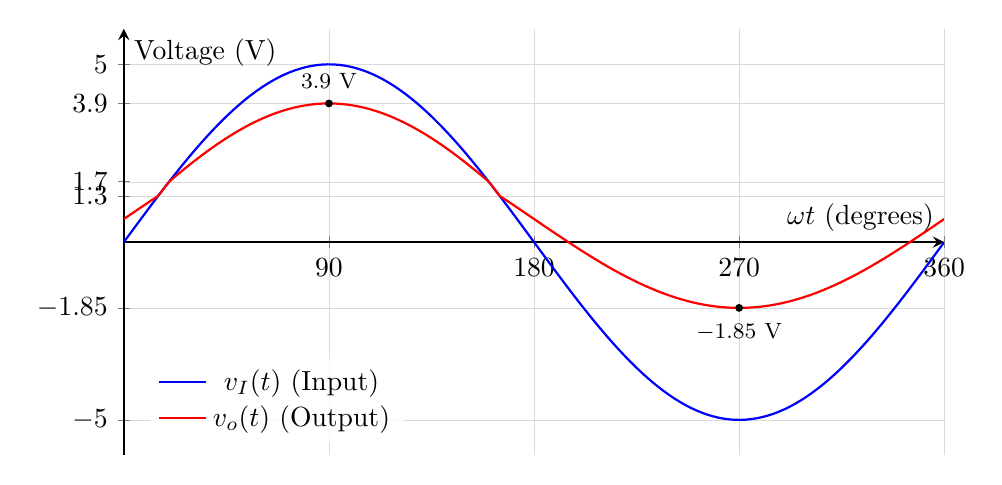
\begin{tikzpicture}
    \begin{axis}[
        width=12cm, height=7cm,
        xmin=0, xmax=360,
        ymin=-6, ymax=6,
        axis lines=center,
        xlabel={$\omega t$ (degrees)},
        ylabel={Voltage (V)},
        xtick={0, 90, 180, 270, 360},
        ytick={-5, -1.85, 0, 1.3, 1.7, 3.9, 5},
        grid=both,
        grid style={line width=.1pt, draw=gray!30},
        legend pos=south west,
        legend style={draw=none, fill=white, fill opacity=0.8, text opacity=1}
    ]
        
    % Input Waveform
    \addplot[blue, thick, domain=0:360, samples=150] {5*sin(x)};
    \addlegendentry{$v_I(t)$ (Input)}
    
    % Output Waveform
    \addplot[red, thick, domain=0:360, samples=300] 
        { (5*sin(x) > 1.7) * (0.66667 * 5*sin(x) + 0.56667) 
        + (5*sin(x) < 1.3) * (0.5 * 5*sin(x) + 0.65) 
        + (5*sin(x) >= 1.3) * (5*sin(x) <= 1.7) * (5*sin(x)) };
    \addlegendentry{$v_o(t)$ (Output)}
    
    % Peak Marks
    \node[label={90:{\footnotesize $3.9\text{ V}$}},circle,fill,inner sep=1pt] at (axis cs:90,3.9) {};
    \node[label={270:{\footnotesize $-1.85\text{ V}$}},circle,fill,inner sep=1pt] at (axis cs:270,-1.85) {};
    
    \end{axis}
\end{tikzpicture}
\end{center}

\end{tcolorbox}

\item Design a limiter circuit using only diodes and 10\,k$\Omega$ resistors to provide an output signal limited to the range $\pm2.1\,\text{V}$. Assume each diode has a 0.7\,V drop when conducting.
\mk{15} \yr{EEE 263 | L-2/T-1 | 2021--22}

\begin{tcolorbox}[enhanced,breakable,ansbox,colback=cA!4,colframe=cA,boxrule=0.8pt,arc=5pt,title={\textbf{Answer}},fonttitle=\bfseries\color{white},colbacktitle=cA]

\subsection*{1. Design Principle and Theory}
A limiter (or clipper) circuit is used to restrict the voltage excursions of an input signal from exceeding predetermined levels. The design requires an output voltage symmetrically limited to $\pm 2.1\text{ V}$, using only resistors of $10\text{ k}\Omega$ and diodes with a constant voltage drop of $V_\gamma = 0.7\text{ V}$.

To achieve a limiting voltage of $2.1\text{ V}$ without external DC biasing sources, we can connect multiple diodes in series. Since each diode provides a $0.7\text{ V}$ drop when forward-biased, the number of diodes required in series is:
\begin{equation*}
    n = \frac{V_{\text{limit}}}{V_\gamma} = \frac{2.1\text{ V}}{0.7\text{ V}} = 3
\end{equation*}
Thus, a string of three diodes connected in series will limit the voltage to $2.1\text{ V}$. 
\begin{itemize}
    \item \textbf{Positive Limiting ($+2.1\text{ V}$):} A string of 3 diodes with anodes facing the output node and cathodes facing ground.
    \item \textbf{Negative Limiting ($-2.1\text{ V}$):} A parallel string of 3 diodes in the reverse orientation (cathodes facing the output node, anodes facing ground).
    \item \textbf{Current Limiting:} A series resistor $R_S = 10\text{ k}\Omega$ is required to drop the excess voltage and limit the current through the diodes when they are conducting.
\end{itemize}

\vspace{0.5cm}

\subsection*{2. Proposed Circuit Diagram}
\begin{center}
    \begin{circuitikz}[thick, american, scale=0.9, transform shape]
        % Input Terminals
        \draw (0,5) node[ocirc]{} node[left]{$v_{in}$} 
              to[R, l=$R_S$, a=$10\text{ k}\Omega$, i=$i_{in}$] (3,5);
        \draw (0,0) node[ocirc]{} node[left]{GND} -- (8,0);
        
        % Vout Node
        \draw (3,5) -- (8,5) node[ocirc]{};
        \draw (8,0) node[ocirc]{};
        
        \node at (8.5, 5) {$+$};
        \node at (8.5, 2.5) {$v_{out}$};
        \node at (8.5, 0) {$-$};
        
        % Branch 1: Positive Limiter (Diodes point down)
        \draw (4,5) node[circ]{} -- (4, 4.5);
        \draw (4, 4.5) to[D, l=$D_1$] (4, 3) 
                       to[D, l=$D_2$] (4, 1.5) 
                       to[D, l=$D_3$] (4, 0);
        \draw (4,0) node[circ]{};
        
        % Branch 2: Negative Limiter (Diodes point up)
        \draw (6,5) node[circ]{} -- (6, 4.5);
        % Drawing from bottom to top so diodes point up
        \draw (6, 0)   to[D, l=$D_6$] (6, 1.5) 
                       to[D, l=$D_5$] (6, 3) 
                       to[D, l=$D_4$] (6, 4.5);
        \draw (6,0) node[circ]{};
        
    \end{circuitikz}
\end{center}

\vspace{0.5cm}

\subsection*{3. Circuit Operation and Mathematical Analysis}
To determine the transfer characteristic, we analyze the operating states of the diodes for different ranges of the input voltage $v_{in}$. We assume the output is open-circuited (no load resistor).

\subsubsection*{Region I: Non-limiting Region ($-2.1\text{ V} < v_{in} < 2.1\text{ V}$)}
\begin{itemize}
    \item \textbf{Assumption:} All diodes ($D_1$ to $D_6$) are OFF.
    \item \textbf{Verification:} For $D_1-D_3$ to turn ON, $v_{out}$ must reach $+2.1\text{ V}$. For $D_4-D_6$ to turn ON, $v_{out}$ must drop to $-2.1\text{ V}$. Since the input voltage magnitude is less than $2.1\text{ V}$, neither string has enough forward bias to overcome the cumulative cut-in voltage.
    \item \textbf{Output Equation:} Because no current flows through $R_S$ ($i_{in} = 0$), there is no voltage drop across $R_S$.
    \begin{equation}
        v_{out} = v_{in}
    \end{equation}
\end{itemize}

\subsubsection*{Region II: Positive Limiting ($v_{in} \ge 2.1\text{ V}$)}
\begin{itemize}
    \item \textbf{Assumption:} Diodes $D_1$, $D_2$, and $D_3$ are ON. Diodes $D_4$, $D_5$, and $D_6$ remain OFF.
    \item \textbf{Verification:} The input tries to drive the output node above $2.1\text{ V}$. The forward-biased string $D_1-D_3$ begins to conduct and clamps the node voltage.
    \item \textbf{Output Equation:} The series combination of $D_1, D_2, D_3$ acts as a constant voltage sink of $3 \times 0.7\text{ V} = 2.1\text{ V}$. The excess voltage is dropped across the $10\text{ k}\Omega$ resistor.
    \begin{equation}
        v_{out} = 2.1\text{ V}
    \end{equation}
    The current supplied by the source is $i_{in} = \frac{v_{in} - 2.1}{10\text{ k}\Omega}$.
\end{itemize}

\subsubsection*{Region III: Negative Limiting ($v_{in} \le -2.1\text{ V}$)}
\begin{itemize}
    \item \textbf{Assumption:} Diodes $D_4$, $D_5$, and $D_6$ are ON. Diodes $D_1$, $D_2$, and $D_3$ remain OFF.
    \item \textbf{Verification:} The input tries to drive the output node below $-2.1\text{ V}$. The string $D_4-D_6$ becomes forward-biased (current flows from ground to $v_{out}$) and clamps the node voltage.
    \item \textbf{Output Equation:} The series combination of $D_4, D_5, D_6$ acts as a constant voltage clamp at $-2.1\text{ V}$.
    \begin{equation}
        v_{out} = -2.1\text{ V}
    \end{equation}
\end{itemize}

\vspace{0.5cm}

\subsection*{4. Transfer Characteristics (Voltage Transfer Curve)}
The relationship between $v_{out}$ and $v_{in}$ (VTC) is plotted below, clearly showing the linear region and the symmetric hard limits at $\pm 2.1\text{ V}$.

\begin{center}
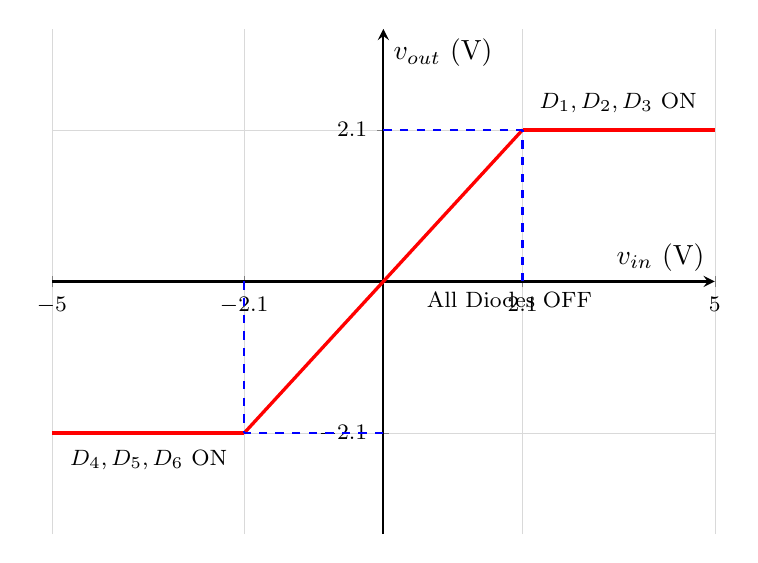
\begin{tikzpicture}
    \begin{axis}[
        width=10cm, height=8cm,
        xmin=-5, xmax=5,
        ymin=-3.5, ymax=3.5,
        axis lines=center,
        xlabel={$v_{in}$ (V)},
        ylabel={$v_{out}$ (V)},
        xtick={-5, -2.1, 2.1, 5},
        ytick={-2.1, 2.1},
        grid=both,
        grid style={line width=.1pt, draw=gray!30},
        axis line style={thick},
        tick label style={font=\footnotesize}
    ]
        
    % Transfer Curve
    \addplot[red, very thick, domain=-5:-2.1, samples=50] {-2.1};
    \addplot[red, very thick, domain=-2.1:2.1, samples=50] {x};
    \addplot[red, very thick, domain=2.1:5, samples=50] {2.1};
    
    % Dashed projection lines
    \draw[dashed, blue] (axis cs:2.1,0) -- (axis cs:2.1,2.1);
    \draw[dashed, blue] (axis cs:0,2.1) -- (axis cs:2.1,2.1);
    \draw[dashed, blue] (axis cs:-2.1,0) -- (axis cs:-2.1,-2.1);
    \draw[dashed, blue] (axis cs:0,-2.1) -- (axis cs:-2.1,-2.1);

    % Labels for Operating Regions
    \node[anchor=south west] at (axis cs: 2.2, 2.2) {\footnotesize $D_1,D_2,D_3$ ON};
    \node[anchor=north east] at (axis cs: -2.2, -2.2) {\footnotesize $D_4,D_5,D_6$ ON};
    \node[anchor=north west] at (axis cs: 0.5, 0) {\footnotesize All Diodes OFF};
    
    \end{axis}
\end{tikzpicture}
\end{center}

\end{tcolorbox}

\item For a sinusoidal input, draw the output waveshape for the circuit shown.
\begin{center}
    \begin{circuitikz}[thick,american, scale=1.2]
    % 1. Top wire with Input terminal, Resistor R, and Output terminal
    \draw (0,2.5) node[below=2pt] {$+$} 
          to[R, l_=$R$, o-*] (3,2.5) 
          to[short, -o] (5,2.5) node[below=2pt] {$+$};
          
    % 2. Bottom reference wire with Input and Output terminals
    \draw (0,0) node[above=2pt] {$-$} 
          to[short, o-*] (3,0) 
          to[short, -o] (5,0) node[above=2pt] {$-$};
          
    % 3. Input and Output Voltage Labels
    \node[font=\large] at (0.5, 1.25) {$V_i$};
    \node[font=\large] at (4.5, 1.25) {$V_o$};
    
    % 4. Shunt Branch: Battery (V) and Diode pointing upwards
    % Drawing from bottom to top automatically sets up the correct polarities
    \draw (3,1.25) to[battery2, l_=$V$] (3,0);
        \draw (3,1.25)  to[D] (3,2.5);
          
    % 5. Figure Caption

\end{circuitikz}
\end{center}
\mk{10} \yr{EEE 263 | L-2/T-1 | 2018--19}

\begin{tcolorbox}[enhanced,breakable,ansbox,colback=cA!4,colframe=cA,boxrule=0.8pt,arc=5pt,title={\textbf{Answer}},fonttitle=\bfseries\color{white},colbacktitle=cA]

\subsection*{1. Circuit Operation and Principle}
The given circuit is a \textbf{biased shunt clipper} (or limiter). It modifies an incoming alternating voltage waveform by cutting off a portion above or below a specific reference level. In this specific configuration:
\begin{itemize}
    \item The diode is placed in a shunt branch with its anode connected towards the output node and its cathode connected to a DC reference voltage source $V$.
    \item Note the orientation of the DC battery: the long bar (positive terminal) is at the top, and the thick short bar (negative terminal) is at the bottom. Therefore, the cathode of the diode is held at a constant potential of $+V$.
    \item We assume an \textbf{ideal diode} model where the forward voltage drop $V_\gamma = 0\text{ V}$ and reverse leakage current is zero.
\end{itemize}

---

\subsection*{2. Analysis of Operating Regions}
To find the output voltage $V_o$ as a function of the input voltage $V_i$, we analyze the state of the diode under different conditions:

\subsubsection*{Case 1: Diode is OFF (Non-Conducting Region)}
\begin{itemize}
    \item \textbf{Assumption:} Assume the diode is reverse-biased (OFF). An ideal open-circuit replaces the diode.
    \item \textbf{Condition for Assumption:} For the diode to remain OFF, the voltage at its anode must be less than the voltage at its cathode:
    \[ V_{\text{anode}} < V_{\text{cathode}} \implies V_i < V \]
    \item \textbf{Output Voltage Calculation:} When the diode is an open circuit, no current flows through the resistor $R$. Therefore, there is no voltage drop across $R$, yielding:
    \[ V_o = V_i \]
    \item \textbf{Verification:} Since $V_o = V_i$, the anode voltage is $V_i$. The condition $V_i < V$ perfectly matches our initial assumption, verifying that the diode remains OFF when $V_i < V$.
\end{itemize}

\subsubsection*{Case 2: Diode is ON (Conducting Region)}
\begin{itemize}
    \item \textbf{Assumption:} Assume the diode is forward-biased (ON). An ideal short-circuit replaces the diode.
    \item \textbf{Condition for Assumption:} The diode turns ON as soon as the input voltage attempts to exceed the cathode potential:
    \[ V_i \ge V \]
    \item \textbf{Output Voltage Calculation:} When the diode behaves as a short-circuit, the output node is directly clamped to the cathode potential established by the reference battery:
    \[ V_o = V \]
    \item \textbf{Circuit Current:} The current flowing through the circuit during this phase is given by Ohm's Law across resistor $R$:
    \[ I_R = \frac{V_i - V}{R} \]
    Since $V_i \ge V$, the current is positive and flows down through the diode, confirming forward bias.
\end{itemize}

---

\subsection*{3. Transfer Characteristic Equation}
Summarizing the two operating regions, the total transfer characteristic function is expressed as:
\begin{equation}
V_o = \begin{cases} 
    V_i & \text{for } V_i < V \\ 
    V & \text{for } V_i \ge V 
\end{cases}
\end{equation}

---

\subsection*{4. Schematic and Waveshape Reconstruction}

\subsubsection*{Circuit Schematic}
\begin{center}
\begin{circuitikz}[thick, american, scale=1.0]
    % Top path
    \draw (0,2.5) node[above=2pt] {$+$} to[short, o-] (0.5,2.5)
          to[R, l=$R$] (3,2.5) 
          to[short, -o] (5,2.5) node[above=2pt] {$+$};
          
    % Bottom path
    \draw (0,0) node[below=2pt] {$-$} to[short, o-*] (3,0) 
          to[short, -o] (5,0) node[below=2pt] {$-$};
          
    % Voltage labels
    \node at (0.2, 1.25) {$V_i$};
    \node at (4.8, 1.25) {$V_o$};
    
    % Shunt Branch
    \draw (3,2.5) to[D, *-] (3,1.25)
          to[battery2, l=$V$] (3,0);
\end{circuitikz}
\end{center}

\subsubsection*{Input and Output Waveshapes}
Below is the precise alignment of the output wave compared to a sinusoidal input of peak amplitude $V_m$ (where $V_m > V$):

\begin{center}
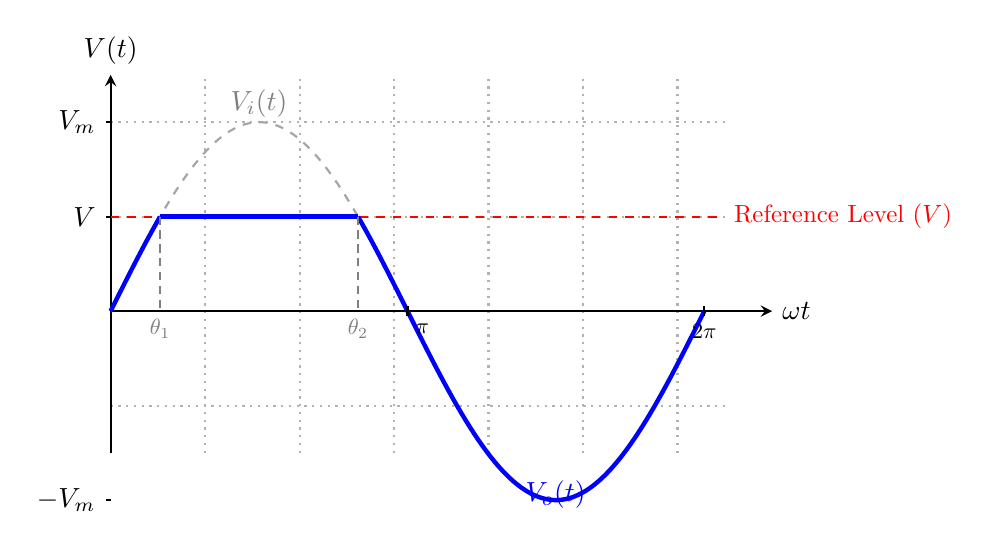
\begin{tikzpicture}[scale=1.2, >=stealth]
    % --- INPUT & OUTPUT WAVEFORMS ---
    % Grid lines
    \draw[dotted, gray!60] (0,-1.5) grid (6.5,2.5);
    
    % Axes
    \draw[->, thick] (0,0) -- (7,0) node[right] {$\omega t$};
    \draw[->, thick] (0,-1.5) -- (0,2.5) node[above] {$V(t)$};
    
    % Reference Voltage Line (V)
    \draw[dashed, red, thick] (0,1) -- (6.5,1) node[right, scale=0.9] {Reference Level ($V$)};
    
    % Input Sinusoid (Light Gray Background Reference)
    \draw[thick, gray!70, dashed, domain=0:6.28, samples=150] plot (\x, {2*sin(\x*180/3.14159)});
    \node[gray] at (1.57, 2.2) {$V_i(t)$};
    
    % Output Clipper Waveform
    % From 0 to theta_1: Vo = Vi
    \draw[ultra thick, blue, domain=0:0.523, samples=50] plot (\x, {2*sin(\x*180/3.14159)});
    % From theta_1 to theta_2: Vo = V
    \draw[ultra thick, blue] (0.523,1) -- (2.618,1);
    % From theta_2 to 2*pi: Vo = Vi
    \draw[ultra thick, blue, domain=2.618:6.283, samples=150] plot (\x, {2*sin(\x*180/3.14159)});
    
    % Labels and Ticks
    \node[blue] at (4.71, -2.2) [above] {\textbf{$V_o(t)$}};
    \draw (0,2) -- (-0.05,2) node[left] {$V_m$};
    \draw (0,-2) -- (-0.05,-2) node[left] {$-V_m$};
    \draw (0,1) -- (-0.05,1) node[left] {$V$};
    
    % Phase Angles
    \draw[densely dashed, gray] (0.523,1) -- (0.523,0) node[below, fill=white, scale=0.8] {$\theta_1$};
    \draw[densely dashed, gray] (2.618,1) -- (2.618,0) node[below, fill=white, scale=0.8] {$\theta_2$};
    \draw (3.141,0.05) -- (3.141,-0.05) node[below right, scale=0.8] {$\pi$};
    \draw (6.283,0.05) -- (6.283,-0.05) node[below, scale=0.8] {$2\pi$};
\end{tikzpicture}
\end{center}

---

\subsection*{5. Important Notes and Key Takeaways}
\begin{itemize}
    \item \textbf{Clipping Action:} This circuit clips off everything \textbf{above} the reference level $V$. It is classified as a Positive Clipper with a positive bias voltage.
    \item \textbf{Angles of Conduction Cutoff:} The clipping region starts at angle $\theta_1 = \arcsin(V/V_m)$ and ends at $\theta_2 = \pi - \theta_1$.
    \item \textbf{Applications:} Used extensively in wave-shaping, noise limiting in FM receivers, and protecting sensitive ADC stages against over-voltage spikes.
\end{itemize}

\end{tcolorbox}

\item Design a parallel-based clipper that will yield the voltage transfer function shown in the figure. Assume 0.7\,V as diode cut-in voltage.
\begin{center}
  
    \begin{tikzpicture}[thick,scale=0.7]
        
        % ==========================================
        % Axes
        % ==========================================
        \draw[-latex, thin] (-7,0) -- (7,0) node[right] {$v_I$};
        \draw[-latex, thin] (0,-7) -- (0,5) node[above] {$v_O$};
        
        % ==========================================
        % VTC Curve
        % ==========================================
        % Region 1: Clipped at -5V
        \draw[very thick] (-7,-5) -- (-5,-5);
        
        % Region 2: Linear region with slope = 1
        \draw[very thick] (-5,-5) -- (2.5,2.5);
        
        % Region 3: Linear region with slope = 1/3
        % Calculation for end point: at x = 7, y = 2.5 + (7 - 2.5)/3 = 4
        \draw[very thick] (2.5,2.5) -- (7,4);
        
        % ==========================================
        % Breakpoints and Dashed Lines
        % ==========================================
        % Lower breakpoint at (-5, -5)
        \draw[dashed] (-5,0) node[above] {$-5$} -- (-5,-5) -- (0,-5) node[right] {$-5$};
        
        % Upper breakpoint at (2.5, 2.5)
        \draw[dashed] (2.5,0) node[below] {$2.5$} -- (2.5,2.5) -- (0,2.5) node[left] {$2.5$};
        
        % ==========================================
        % Slope Indicator Triangle
        % ==========================================
        % Drawing a triangle with run = 3 and rise = 1
        % Starting at x = 3.5. 
        % y at 3.5 = 2.5 + (3.5 - 2.5)/3 = 2.833
        \draw (3.5, 2.833) -- (6.5, 2.833) node[midway, below] {$3$} -- (6.5, 3.833) node[midway, right] {$1$};
        
    \end{tikzpicture}
\end{center}
\mk{18} \yr{EEE 263 | L-2/T-1 | 2017--18}

\begin{tcolorbox}[enhanced,breakable,ansbox,colback=cA!4,colframe=cA,boxrule=0.8pt,arc=5pt,title={\textbf{Answer}},fonttitle=\bfseries\color{white},colbacktitle=cA]

\subsection*{1. Analysis of the Voltage Transfer Characteristic (VTC)}
The given VTC can be divided into three distinct regions of operation:
\begin{itemize}
    \item \textbf{Region 1 (Negative Hard Clipping):} For $v_I \le -5\,\text{V}$, the output is clipped at $v_O = -5\,\text{V}$. The slope is $0$. This implies a parallel diode branch without a series resistor that turns ON when the output tries to drop below $-5\,\text{V}$.
    \item \textbf{Region 2 (Linear Operation):} For $-5\,\text{V} < v_I < 2.5\,\text{V}$, the output strictly follows the input ($v_O = v_I$). The slope is $1$. All diode branches must be OFF (open-circuited) in this region.
    \item \textbf{Region 3 (Positive Soft Clipping):} For $v_I \ge 2.5\,\text{V}$, the output increases with a slope of $1/3$. This implies a parallel diode branch with a series resistor that turns ON, creating a voltage divider with the main series input resistor.
\end{itemize}

\subsection*{2. Circuit Design \& Parameter Selection}
We must design a parallel clipper consisting of a main series resistor $R$ and two parallel clipping branches. We are given the diode cut-in voltage $V_\gamma = 0.7\,\text{V}$.

\subsubsection*{Step 2.1: Positive Soft-Clipping Branch (Region 3)}
This branch controls the VTC for $v_I \ge 2.5\,\text{V}$. It consists of a resistor $R_1$ in series with a diode $D_1$ pointing downwards (anode at the top) and a DC reference voltage $V_{R1}$.
\begin{itemize}
    \item \textbf{Slope Condition:} When $D_1$ is ON, $R$ and $R_1$ form a voltage divider. The slope is determined by:
    \begin{equation}
        \text{Slope} = \frac{R_1}{R + R_1} = \frac{1}{3} \implies 3R_1 = R + R_1 \implies R = 2R_1
    \end{equation}
    Let us select standard resistor values: \textbf{$R_1 = 10\,\text{k}\Omega$} and \textbf{$R = 20\,\text{k}\Omega$}.
    
    \item \textbf{Turn-ON Condition:} The branch must start conducting when $v_O = 2.5\,\text{V}$. The diode turns ON when its anode-to-cathode voltage reaches $0.7\,\text{V}$.
    \begin{equation}
        v_O - V_{R1} = 0.7\,\text{V} \implies 2.5\,\text{V} - V_{R1} = 0.7\,\text{V} \implies \mathbf{V_{R1} = 1.8\,\text{V}}
    \end{equation}
\end{itemize}

\subsubsection*{Step 2.2: Negative Hard-Clipping Branch (Region 1)}
This branch controls the VTC for $v_I \le -5\,\text{V}$. Since the slope is 0, the branch resistance $R_2 = 0\,\Omega$. It consists of a diode $D_2$ pointing upwards (cathode at the top) and a DC reference voltage $V_{R2}$.
\begin{itemize}
    \item \textbf{Turn-ON Condition:} The branch must conduct when $v_O$ attempts to drop below $-5\,\text{V}$. $D_2$ turns ON when its anode-to-cathode voltage reaches $0.7\,\text{V}$.
    \begin{equation}
        V_{R2} - v_O = 0.7\,\text{V} \implies V_{R2} - (-5\,\text{V}) = 0.7\,\text{V} \implies \mathbf{V_{R2} = -4.3\,\text{V}}
    \end{equation}
    A negative reference voltage of $-4.3\,\text{V}$ can be implemented by reversing the polarity of a $4.3\,\text{V}$ DC source (connecting its positive terminal to ground).
\end{itemize}

\subsection*{3. Proposed Circuit Diagram}
\begin{center}
    \begin{circuitikz}[american, thick, scale=1.0, transform shape]
        
        % Main Input and Series Resistor
        \draw (0,4) node[ocirc]{} node[left]{$v_I$} 
              to[R, l={$R=20\,\text{k}\Omega$}, i=$i_I$] (4,4);
        \draw (0,0) node[ocirc]{} node[left]{GND} -- (9,0);
        
        % Vout Terminals
        \draw (4,4) -- (9,4) node[ocirc]{};
        \draw (9,0) node[ocirc]{};
        \node at (9.5, 4) {$+$};
        \node at (9.5, 2) {$v_O$};
        \node at (9.5, 0) {$-$};
        
        % Branch 1: Positive Soft-Clipper
        \draw (5,4) node[circ]{} to[R, l={$R_1=10\,\text{k}\Omega$}] (5,2.5)
                    to[D, l=$D_1$] (5,1.2);
        % Battery for V_R1: Positive up, Negative down
        \draw (5,0) node[circ]{} to[battery1, l={$1.8\,\text{V}$}] (5,1.2);
        
        % Branch 2: Negative Hard-Clipper
        % Diode D2 points UP (Anode bottom, Cathode top)
        \draw (7,1.5) to[D, l=$D_2$] (7,4) node[circ]{};
        % Battery for V_R2: Negative up, Positive down (to get -4.3V at anode)
        \draw (7,1.5) to[battery1, l=$4.3\,\text{V}$] (7,0) node[circ]{};
        
    \end{circuitikz}
\end{center}

\subsection*{4. Mathematical Verification}
Let's verify the designed circuit against the three regions of operation using Nodal Analysis (KCL) at node $v_O$:

\textbf{Case 1: $v_I \le -5\,\text{V}$ ($D_1$ OFF, $D_2$ ON)} \\
Diode $D_2$ is forward-biased and acts as a $0.7\,\text{V}$ source. 
\begin{equation}
    v_O = V_{R2} - V_\gamma = -4.3\,\text{V} - 0.7\,\text{V} = -5.0\,\text{V}
\end{equation}
This confirms the flat clipping at $-5\,\text{V}$ (Slope $= 0$).

\vspace{0.3cm}

\textbf{Case 2: $-5\,\text{V} < v_I < 2.5\,\text{V}$ ($D_1$ OFF, $D_2$ OFF)} \\
Both diodes are reverse-biased and act as open circuits. No current flows through the series resistor $R$ ($i_I = 0$).
\begin{equation}
    v_O = v_I - i_I R = v_I - 0 = v_I
\end{equation}
This confirms the linear region with a slope of $1$.

\vspace{0.3cm}

\textbf{Case 3: $v_I \ge 2.5\,\text{V}$ ($D_1$ ON, $D_2$ OFF)} \\
Diode $D_1$ is forward-biased and acts as a $0.7\,\text{V}$ source. The $D_1$ branch can be modeled as a voltage source $V_{eq} = 1.8\,\text{V} + 0.7\,\text{V} = 2.5\,\text{V}$ in series with $R_1 = 10\,\text{k}\Omega$. Applying KCL at the $v_O$ node:
\begin{align*}
    \frac{v_O - v_I}{20} + \frac{v_O - 2.5}{10} &= 0 \\
    (v_O - v_I) + 2(v_O - 2.5) &= 0 \\
    3v_O - v_I - 5 &= 0 \\
    3v_O &= v_I + 5 \\
    v_O &= \frac{1}{3}v_I + \frac{5}{3}
\end{align*}
The output equation clearly has a slope of $1/3$. Furthermore, exactly at the boundary $v_I = 2.5\,\text{V}$:
\begin{equation}
    v_O = \frac{1}{3}(2.5) + \frac{5}{3} = \frac{7.5}{3} = 2.5\,\text{V}
\end{equation}
This perfectly matches the target Voltage Transfer Characteristic.

\end{tcolorbox}

\item For the circuit shown in Figure ,  find and sketch the voltage transfer characteristics with proper labelling. Utilize the constant-voltage drop model ($0.7\text{ V}$) for each conduction diode.  

\begin{center}
        \begin{circuitikz}[thick , transform shape]
            
            % ==========================================
            % Define Main Bridge Coordinates
            % ==========================================
            \coordinate (NodeL) at (2, 4);
            \coordinate (NodeR) at (6, 4);
            \coordinate (NodeT) at (4, 6);
            \coordinate (NodeB) at (4, 2);
    
            % ==========================================
            % Diode Bridge
            % ==========================================
            % Top to Left (D1) and Top to Right (D2)
            \draw (NodeT) to[D, l_=$D_1$] (NodeL);
            \draw (NodeT) to[D, l=$D_2$] (NodeR);
    
            % Left to Bottom (D3) and Right to Bottom (D4)
            \draw (NodeL) to[D, l_=$D_3$] (NodeB);
            \draw (NodeR) to[D, l=$D_4$] (NodeB);
    
            % Junction dots for the bridge
            \node[circ] at (NodeL) {};
            \node[circ] at (NodeR) {};
            \node[circ] at (NodeT) {};
            \node[circ] at (NodeB) {};
    
            % ==========================================
            % Top and Bottom Bias Paths
            % ==========================================
            % +10V Pull-up
            \draw (NodeT) to[R, l=$10\text{ k}\Omega$] (4, 8);
            \draw[-latex, thick] (4, 8) -- (4, 8.8) node[above] {$+10\text{V}$};
    
            % -10V Pull-down
            \draw (NodeB) to[R, l=$10\text{ k}\Omega$] (4, 0);
            \draw[-latex, thick] (4, 0) -- (4, -0.8) node[below] {$-10\text{V}$};
    
            % ==========================================
            % Input Stage (Left)
            % ==========================================
            % AC Source vi to ground
            \draw (NodeL) -- (0.5, 4) to[sV, l_=$v_i$] (0.5, 2) node[ground] {};
    
            % ==========================================
            % Output Stage (Right)
            % ==========================================
            % Output label vo
            \draw (NodeR) -- (8.5, 4) node[ocirc] {} node[right] {\Large $v_o$};
            
            % 10k Output Resistor to ground
            \draw (7.5, 4) node[circ] {} to[R, l=$10\text{ k}\Omega$] (7.5, 2) node[ground] {};
    
          
        \end{circuitikz}
\end{center}
\mk{13} \yr{EEE 263 | L-2/T-1 | 2016--17}

\begin{tcolorbox}[enhanced,breakable,ansbox,colback=cA!4,colframe=cA,boxrule=0.8pt,arc=5pt,title={\textbf{Answer}},fonttitle=\bfseries\color{white},colbacktitle=cA]

\subsection*{1. Circuit Overview and Operating Principle}
The given circuit is a \textbf{diode bridge limiter} (or clipper). It utilizes a symmetrical diode bridge ($D_1$ to $D_4$) biased by $\pm 10\text{ V}$ DC sources through $10\text{ k}\Omega$ resistors. The output voltage $v_o$ is taken across a $10\text{ k}\Omega$ load resistor. We will analyze the circuit using the constant-voltage drop model for the diodes, where $V_\gamma = 0.7\text{ V}$.

Let us define the nodes:
\begin{itemize}
    \item \textbf{Input Node (Left):} Driven directly by $v_i$.
    \item \textbf{Output Node (Right):} Voltage is $v_o$.
    \item \textbf{Top Node:} Voltage is $V_T$, connected to $+10\text{ V}$ via $10\text{ k}\Omega$.
    \item \textbf{Bottom Node:} Voltage is $V_B$, connected to $-10\text{ V}$ via $10\text{ k}\Omega$.
\end{itemize}

\vspace{0.5cm}

\subsection*{2. Analysis of Operating Regions}

\subsubsection*{Region I: Linear Operation (All Diodes ON)}
For small values of input voltage $v_i$, the $\pm 10\text{ V}$ sources keep all four diodes forward-biased.
\begin{itemize}
    \item With $D_1$ and $D_3$ ON, the top and bottom node voltages are clamped to the input:
    \begin{equation}
        V_T = v_i + 0.7\text{ V}, \quad V_B = v_i - 0.7\text{ V}
    \end{equation}
    \item With $D_2$ and $D_4$ ON, the output voltage is dictated by $V_T$ and $V_B$:
    \begin{equation}
        v_o = V_T - 0.7\text{ V} = (v_i + 0.7\text{ V}) - 0.7\text{ V} = v_i
    \end{equation}
    Thus, in this region, the output strictly follows the input: $\mathbf{v_o = v_i}$.
\end{itemize}

To find the upper limit of this region, we determine when diodes $D_1$ and $D_4$ turn OFF (currents reach zero). 
By applying Kirchhoff's Current Law (KCL) at the top and bottom nodes, the total currents supplied are:
\begin{align*}
    I_T &= \frac{10 - V_T}{10\text{ k}\Omega} = \frac{9.3 - v_i}{10\text{ k}\Omega} \\
    I_B &= \frac{V_B - (-10)}{10\text{ k}\Omega} = \frac{v_i + 9.3}{10\text{ k}\Omega}
\end{align*}
At the upper breakpoint ($v_i > 0$), $D_1$ and $D_4$ turn off simultaneously. When this happens, all top current flows through $D_2$ to the output, and no current flows through $D_4$. Setting the current through $D_4$ to zero:
\begin{equation}
    I_{D4} = 0 \implies I_{D2} = I_L = \frac{v_o}{10\text{ k}\Omega} = \frac{v_i}{10\text{ k}\Omega}
\end{equation}
Since $I_T = I_{D1} + I_{D2}$ and $I_{D1} = 0$:
\begin{equation}
    \frac{9.3 - v_i}{10\text{ k}\Omega} = \frac{v_i}{10\text{ k}\Omega} \implies 9.3 - v_i = v_i \implies 2v_i = 9.3 \implies \mathbf{v_i = 4.65\text{ V}}
\end{equation}
By symmetry, the lower breakpoint occurs at $\mathbf{v_i = -4.65\text{ V}}$.

\vspace{0.3cm}

\subsubsection*{Region II: Positive Clipping ($v_i \ge 4.65\text{ V}$)}
When $v_i$ exceeds $4.65\text{ V}$, $D_1$ and $D_4$ are reverse-biased (OFF). $D_2$ and $D_3$ remain ON. 
The output node is now isolated from the input and is only driven by the $+10\text{ V}$ source through the top $10\text{ k}\Omega$ resistor and $D_2$.
Applying KCL at the output node ($v_o$):
\begin{align*}
    \frac{10 - (v_o + 0.7)}{10\text{ k}\Omega} &= \frac{v_o}{10\text{ k}\Omega} \\
    9.3 - v_o &= v_o \\
    2v_o &= 9.3 \implies \mathbf{v_o = 4.65\text{ V}}
\end{align*}
The output is clamped at $+4.65\text{ V}$.

\vspace{0.3cm}

\subsubsection*{Region III: Negative Clipping ($v_i \le -4.65\text{ V}$)}
When $v_i$ drops below $-4.65\text{ V}$, $D_2$ and $D_3$ turn OFF. $D_1$ and $D_4$ remain ON.
The output node is driven by the $-10\text{ V}$ source through the bottom $10\text{ k}\Omega$ resistor and $D_4$.
Applying KCL at the output node ($v_o$):
\begin{align*}
    \frac{v_o}{10\text{ k}\Omega} + \frac{v_o - 0.7 - (-10)}{10\text{ k}\Omega} &= 0 \\
    v_o + v_o + 9.3 &= 0 \\
    2v_o &= -9.3 \implies \mathbf{v_o = -4.65\text{ V}}
\end{align*}
The output is clamped at $-4.65\text{ V}$.

\vspace{0.5cm}

\subsection*{3. Voltage Transfer Characteristic (VTC)}
The transfer curve exhibits a linear region with a slope of 1 for input voltages between $-4.65\text{ V}$ and $+4.65\text{ V}$, and hard limits (slope 0) outside this range.

\begin{center}
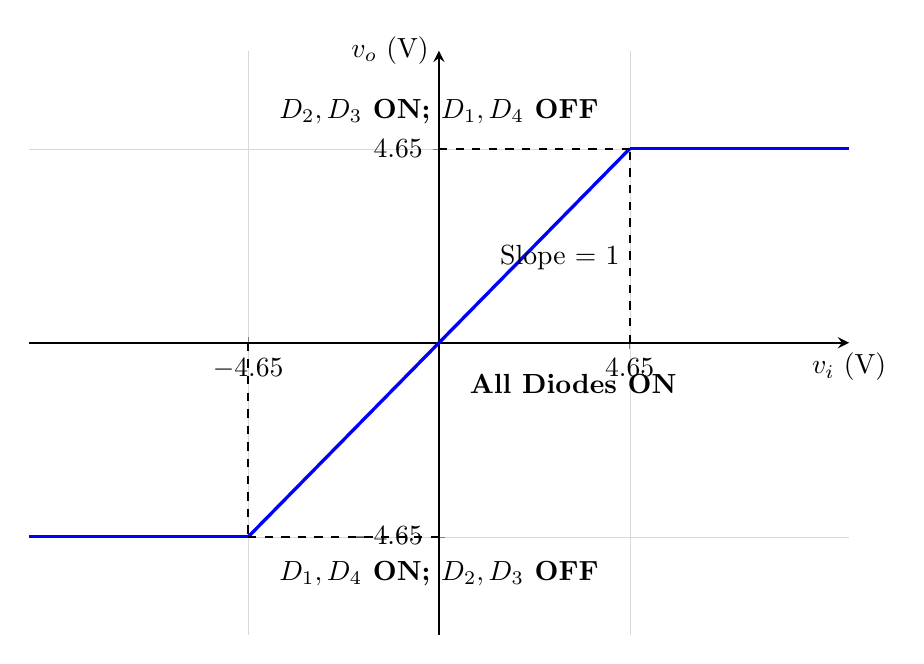
\begin{tikzpicture}
    \begin{axis}[
        width=12cm, height=9cm,
        xmin=-10, xmax=10,
        ymin=-7, ymax=7,
        axis lines=center,
        xlabel={$v_i$ (V)},
        ylabel={$v_o$ (V)},
        xtick={-4.65, 4.65},
        ytick={-4.65, 4.65},
        grid=both,
        grid style={line width=.1pt, draw=gray!30},
        axis line style={thick},
        tick label style={font=\normalsize},
        xlabel style={anchor=north},
        ylabel style={anchor=east}
    ]
        
    % Transfer Curve
    \addplot[blue, very thick, domain=-10:-4.65, samples=50] {-4.65};
    \addplot[blue, very thick, domain=-4.65:4.65, samples=50] {x};
    \addplot[blue, very thick, domain=4.65:10, samples=50] {4.65};
    
    % Dashed projection lines
    \draw[dashed, black, thick] (axis cs:4.65,0) -- (axis cs:4.65,4.65);
    \draw[dashed, black, thick] (axis cs:0,4.65) -- (axis cs:4.65,4.65);
    \draw[dashed, black, thick] (axis cs:-4.65,0) -- (axis cs:-4.65,-4.65);
    \draw[dashed, black, thick] (axis cs:0,-4.65) -- (axis cs:-4.65,-4.65);

    % Labels for Operating Regions
    \node[anchor=south] at (axis cs: 0, 5) {\textbf{$D_2, D_3$ ON; $D_1, D_4$ OFF}};
    \node[anchor=north] at (axis cs: 0, -5) {\textbf{$D_1, D_4$ ON; $D_2, D_3$ OFF}};
    \node[anchor=north west] at (axis cs: 0.5, -0.5) {\textbf{All Diodes ON}};
    \node[anchor=south east] at (axis cs: 4.65, 1.5) {Slope = $1$};
    
    \end{axis}
\end{tikzpicture}
\end{center}

\end{tcolorbox}

\item For the circuit shown, neatly draw the output ($v_o$) waveform corresponding to the input ($v_{in}$). Here, $v_{in}=10\sin(200\pi t)$ and diodes are non-ideal.
\begin{center}
  
    \begin{circuitikz}[thick,scale=1.2, transform shape, y=1.7cm]
        
        % ১. AC Source (Left Side)
        \draw (0,0) to[sV] (0,3);
        \node at (-1, 1.5) {$(v_{in})$};
        \node at (-0.4, 2.3) {$+$};
        \node at (-0.4, 0.7) {$-$};
        
        % ২. Series Resistor (Top Wire)
        \draw (0,3) to[R, l={$10\mathrm{K}$}] (3,3);
        \draw ( 3,3) -- (5.5,3);
        % ৩. Left Parallel Branch (Diode Upwards)
        \draw (3,0) to[R, l={$5\mathrm{K}$}] (3,1);
        \draw (3,1) to[battery1] (3,2); 
        \draw (3,2) to[empty diode] (3,3);
        
        % Left Battery Labels
        \node at (2.3, 1.5) {$5\mathrm{V}$};
        \node at (2.6, 1.8) {$-$}; % মাইনাস উপরে
        \node at (2.6, 1.2) {$+$}; % প্লাস নিচে
        
        % ৪. Right Parallel Branch (Diode Downwards)
        \draw (5.5,3) to[empty diode] (5.5,2);
        \draw (5.5,2) to[battery1] (5.5,1);
        \draw (5.5,1) to[R, l={$20\mathrm{K}$}] (5.5,0);
        
        % Right Battery Labels
        \node at (6.2, 1.5) {$5\mathrm{V}$};
        \node at (5.9, 1.8) {$+$}; % প্লাস উপরে
        \node at (5.9, 1.2) {$-$}; % মাইনাস নিচে
        
        % ৫. Bottom Wire
        \draw (0,0) -- (5.5,0);
        
        % ৬. Junction Dots (কানেকশন পয়েন্ট)
        \fill (3,3) circle (1.5pt);
        \fill (3,0) circle (1.5pt);
        \fill (5.5,3) circle (1.5pt);
        \fill (5.5,0) circle (1.5pt);
        
        % ৭. Output Terminals (Right Side)
        \draw (5.5,3) to[short, -o] (7.5,3);
        \draw (5.5,0) to[short, -o] (7.5,0);
        
        \node[right] at (7.6, 3) {$+$};
        \node[right] at (7.6, 1.5) {$V_o$};
        \node[right] at (7.6, 0) {$-$};
        
    \end{circuitikz}
\end{center}
\mk{16} \yr{EEE 263 | L-2/T-1 | 2015--16}

\begin{tcolorbox}[enhanced,breakable,ansbox,colback=cA!4,colframe=cA,boxrule=0.8pt,arc=5pt,title={\textbf{Answer}},fonttitle=\bfseries\color{white},colbacktitle=cA]

\subsection*{1. Circuit Analysis and Operating Regions}
The circuit consists of an AC input source $v_{in} = 10\sin(200\pi t)$ and two parallel soft-clipping branches. We assume a non-ideal constant voltage drop model for the diodes, where $V_\gamma = 0.7\text{ V}$.

Let's determine the turn-on conditions for each branch:
\begin{itemize}
    \item \textbf{Right Branch ($D_2$):} The diode points downwards. The cathode is connected to a $+5\text{ V}$ potential (battery positive terminal up) relative to ground (assuming zero initial current). $D_2$ turns ON when $v_o - 5\text{ V} \ge 0.7\text{ V}$, which means $\mathbf{v_o \ge 5.7\text{ V}}$.
    \item \textbf{Left Branch ($D_1$):} The diode points upwards. The anode is connected to a $-5\text{ V}$ potential (battery negative terminal up). $D_1$ turns ON when $-5\text{ V} - v_o \ge 0.7\text{ V}$, which means $\mathbf{v_o \le -5.7\text{ V}}$.
\end{itemize}

Based on these thresholds, the circuit operates in three distinct regions:

\subsubsection*{Region I: Linear Region ($-5.7\text{ V} < v_{in} < 5.7\text{ V}$)}
Both $D_1$ and $D_2$ are OFF. No current flows through the $10\text{ k}\Omega$ series resistor, so there is no voltage drop across it. 
\begin{equation}
    v_o = v_{in}
\end{equation}

\subsubsection*{Region II: Positive Soft-Clipping ($v_{in} \ge 5.7\text{ V}$)}
$D_2$ is ON, and $D_1$ is OFF. The right branch conducts, and we apply KCL at the output node ($v_o$):
\begin{align*}
    \frac{v_{in} - v_o}{10\text{ k}\Omega} &= \frac{v_o - 0.7 - 5}{20\text{ k}\Omega} \\
    2(v_{in} - v_o) &= v_o - 5.7 \\
    2v_{in} - 2v_o &= v_o - 5.7 \\
    3v_o &= 2v_{in} + 5.7 \implies \mathbf{v_o = \frac{2}{3}v_{in} + 1.9\text{ V}}
\end{align*}
The peak input is $v_{in(peak)} = 10\text{ V}$. At this peak, $v_o = \frac{2}{3}(10) + 1.9 = \mathbf{8.57\text{ V}}$.

\subsubsection*{Region III: Negative Soft-Clipping ($v_{in} \le -5.7\text{ V}$)}
$D_1$ is ON, and $D_2$ is OFF. The left branch conducts. Applying KCL at the output node ($v_o$):
\begin{align*}
    \frac{v_{in} - v_o}{10\text{ k}\Omega} + \frac{-5 - 0.7 - v_o}{5\text{ k}\Omega} &= 0 \\
    (v_{in} - v_o) + 2(-5.7 - v_o) &= 0 \\
    v_{in} - v_o - 11.4 - 2v_o &= 0 \\
    3v_o &= v_{in} - 11.4 \implies \mathbf{v_o = \frac{1}{3}v_{in} - 3.8\text{ V}}
\end{align*}
The minimum input is $v_{in(min)} = -10\text{ V}$. At this trough, $v_o = \frac{1}{3}(-10) - 3.8 = \mathbf{-7.13\text{ V}}$.

\vspace{0.5cm}

\subsection*{2. Output Waveform Sketch}
The input is $v_{in} = 10\sin(200\pi t)$, which has a frequency $f = 100\text{ Hz}$ and a time period $T = 10\text{ ms}$.

\begin{center}
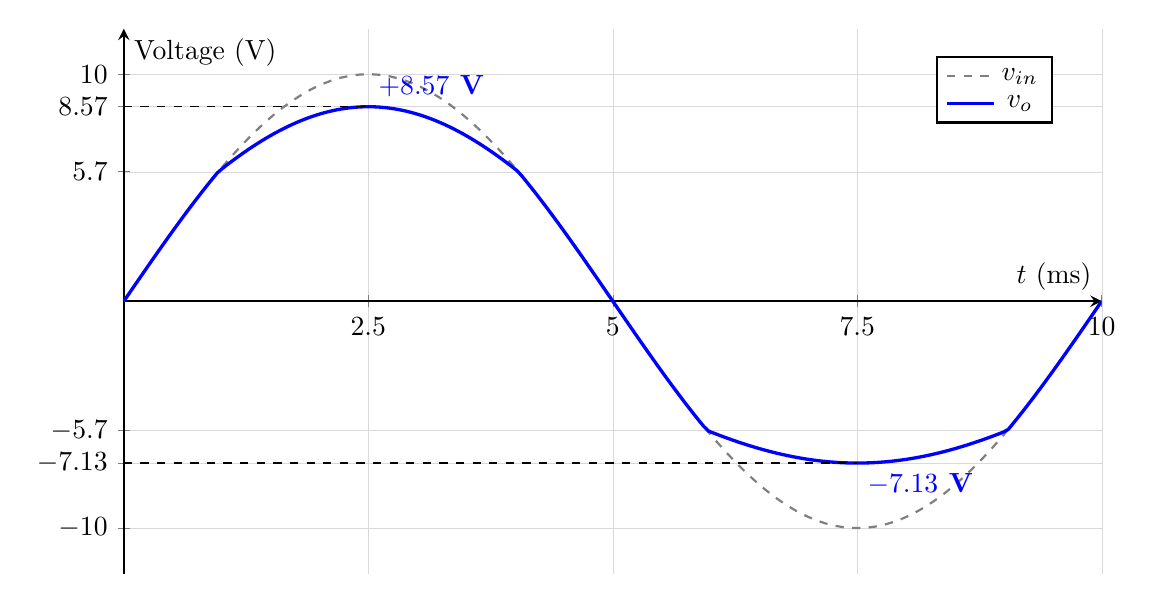
\begin{tikzpicture}
    \begin{axis}[
        width=14cm, height=8.5cm,
        xmin=0, xmax=10,
        ymin=-12, ymax=12,
        axis lines=center,
        xlabel={$t$ (ms)},
        ylabel={Voltage (V)},
        xtick={2.5, 5, 7.5, 10},
        ytick={-10, -7.13, -5.7, 5.7, 8.57, 10},
        grid=both,
        grid style={line width=.1pt, draw=gray!30},
        axis line style={thick},
        tick label style={font=\normalsize},
        legend style={at={(0.95,0.95)},anchor=north east},
        declare function={
            vin(\t) = 10*sin(36*\t);
            vout(\t) = vin(\t) > 5.7 ? (2/3)*vin(\t) + 1.9 : (vin(\t) < -5.7 ? (1/3)*vin(\t) - 3.8 : vin(\t));
        }
    ]
        
    % Input Waveform
    \addplot[dashed, gray, thick, domain=0:10, samples=100] {vin(x)};
    \addlegendentry{$v_{in}$}
    
    % Output Waveform
    \addplot[blue, very thick, domain=0:10, samples=200] {vout(x)};
    \addlegendentry{$v_o$}

    % Annotations for peaks and clipping points
    \draw[dashed, black, thin] (axis cs: 0, 8.57) -- (axis cs: 2.5, 8.57);
    \draw[dashed, black, thin] (axis cs: 0, -7.13) -- (axis cs: 7.5, -7.13);
    
    \node[anchor=south west, text=blue] at (axis cs: 2.5, 8.57) {\textbf{$+8.57\text{ V}$}};
    \node[anchor=north west, text=blue] at (axis cs: 7.5, -7.13) {\textbf{$-7.13\text{ V}$}};

    \end{axis}
\end{tikzpicture}
\end{center}

\end{tcolorbox}

\item Assuming that the diodes are ideal, find the output voltage $V_o$ for the circuit given. Draw the wave shape clearly.
\begin{center}
  
    \begin{circuitikz}[thick,scale=1.1]
        
        % ===================================================
        % 1. Left Side: Input Voltage Waveform (Graph)
        % ===================================================
        \coordinate (Origin) at (0,0);
        
        % Y-axis & X-axis
        \draw[->, >=stealth] (Origin |- 0,-2) -- (Origin |- 0,2) node[above] {$v_{in}(\mathrm{Volt})$};
        \draw[->, >=stealth] (Origin) -- (5,0) node[right] {$t(\mathrm{ms})$};
        
        % Y-axis Labels (+10 and -10)
        \draw (-0.1, 1.5) -- (0.1, 1.5) node[left=0.2cm] {$+10$};
        \draw (-0.1, -1.5) -- (0.1, -1.5) node[left=0.2cm] {$-10$};
        
        % Dashed guidelines for peaks
        \draw[dashed] (0, 1.5) -- (1.25, 1.5);
        \draw[dashed] (0, -1.5) -- (3.75, -1.5);
        
        % Triangular Waveform
        \draw[thick] (0,0) -- (1.25, 1.5) 
                     -- (2.5, 0) node[below, yshift=-0.1cm] {$5$} 
                     -- (3.75, -1.5) 
                     -- (5, 0) node[below] {$10$};
                     
        % Label Vin near the axis end as in the image
        
        
    \end{circuitikz}
\end{center}

\begin{center}
    
    \begin{circuitikz}
        % ===================================================
        % 2. Right Side: Circuit Diagram
        % ===================================================
        % Shift the starting point of the circuit to the right to avoid overlap
        \coordinate (C_offset) at (8.5, 0); 
        
        % AC Voltage Source
        \draw (C_offset |- 0,-1.5) to[sV, l={$v_{in}$}] (C_offset |- 0,1.5) coordinate (TopLeft);
        
        % Resistor R at the top
        \draw (TopLeft) to[R, l={$R=10\Omega$}] ++(2.5, 0) coordinate (Node1);
        
        % Branch 1: D1 (pointing down) and 6V Battery (positive/long line UP)
        % l_ moves the labels to the left side of this branch
        \draw (Node1) to[D, l_={$D1$}] ++(0, -1.5) 
                      to[battery1, l_={$6\mathrm{V}$}] ++(0, -1.5) coordinate (Bot1);
        
        % Branch 2: D2 (pointing UP) and 4V Battery (negative/short line UP)
        % Increased distance between branches (from 1.5 to 2.0)
        \draw (Node1) -- ++(2.0, 0) coordinate (Node2);
        \coordinate (Bot2) at (Node2 |- Bot1);
        
        % Drawn from bottom to top. l_ moves labels to the right side of this branch
        \draw (Bot2) to[battery1, l_={$4\mathrm{V}$}] ++(0, 1.5) 
                     to[D, l_={$D2$}] (Node2); 
        
        % Branch 3: Series Capacitor C
        \draw (Node2) to[C, l={$C$}] ++(2, 0) coordinate (Node3);
        
        % Branch 4: D3 (pointing UP)
        \coordinate (Bot3) at (Node3 |- Bot1);
        \draw (Bot3) to[D, l_={$D3$}] (Node3);
        
        % Output Terminals (Vo) 
        % Extended the wire to 1.5 to move Vo further right
        \draw (Node3) to[short, -o] ++(1.5, 0) coordinate (OutTop);
        \draw (Bot3) to[short, -o] ++(1.5, 0) coordinate (OutBot);
        
        % Output Voltage Label (+ and - with Vo)
        \draw (OutTop) to[open, v^={$V_o$}] (OutBot);
        
        % Connect all bottom ground/return wires
        \draw (C_offset |- 0,-1.5) -- (OutBot);
        
    \end{circuitikz}
\end{center}
\mk{20} \yr{EEE 263 | L-2/T-1 | 2014--15}

\begin{tcolorbox}[enhanced,breakable,ansbox,colback=cA!4,colframe=cA,boxrule=0.8pt,arc=5pt,title={\textbf{Answer}},fonttitle=\bfseries\color{white},colbacktitle=cA]

\subsection*{1. Theory and Principle of Circuit Operation}
The given circuit is a combination of two distinct wave-shaping stages operating in cascade:
\begin{enumerate}
    \item \textbf{Stage 1: A Double-Action Clipper (Slicer).} The first section of the circuit, consisting of the resistor $R$, diodes $D1$ and $D2$, and their associated DC bias batteries, acts as a slicer. It limits the intermediate voltage $v_A$ (the node before the capacitor) to a specific upper and lower bound.
    \item \textbf{Stage 2: A Positive Clamper.} The second section, consisting of capacitor $C$ and diode $D3$, acts as a clamping circuit. It adds a DC shift to the clipped waveform so that the lowest peak of the output voltage $V_o$ is firmly clamped to $0\text{V}$.
\end{enumerate}

\textbf{Ideal Assumptions:} 
We assume all diodes are ideal ($V_\gamma = 0\text{V}$, infinite reverse resistance) and the capacitor $C$ is sufficiently large such that its discharge time constant is much greater than the signal period, allowing it to act as a perfect DC voltage source in steady state.

---

\subsection*{2. Step-by-Step Mathematical Derivation}

\subsubsection*{Stage 1: Analysis of the Clipper (Voltage $v_A$)}
Let $v_A$ be the voltage at the node between $R$ and $C$. 
\begin{itemize}
    \item \textbf{Positive Clipping:} Diode $D1$ points downwards, with its cathode connected to the positive terminal of the $6\text{V}$ battery. $D1$ turns ON when $v_A \ge 6\text{V}$. When $D1$ conducts, it acts as a short circuit, and $v_A$ is clamped to a maximum of $\mathbf{+6\text{V}}$.
    \item \textbf{Negative Clipping:} Diode $D2$ points upwards. The battery below it has its shorter (thicker) line on top, indicating its negative terminal is facing up. Therefore, the anode of $D2$ is biased at $-4\text{V}$. $D2$ turns ON when $v_A \le -4\text{V}$. When $D2$ conducts, $v_A$ is clamped to a minimum of $\mathbf{-4\text{V}}$.
    \item \textbf{Linear Region:} For $-4\text{V} < v_{in} < 6\text{V}$, both $D1$ and $D2$ are OFF (open circuit). Assuming negligible charging current flows through $R$ in steady state, $v_A(t) = v_{in}(t)$.
\end{itemize}

Based on the input $v_{in}(t)$ which is a triangular wave ranging from $+10\text{V}$ to $-10\text{V}$, the intermediate voltage $v_A(t)$ will be a clipped triangle wave varying between $\mathbf{+6\text{V}}$ and $\mathbf{-4\text{V}}$.

\subsubsection*{Stage 2: Analysis of the Clamper (Voltage $V_o$)}
The clipped signal $v_A(t)$ is fed into the clamper circuit.
\begin{itemize}
    \item By Kirchhoff's Voltage Law (KVL): $V_o = v_A - V_C$, where $V_C$ is the voltage stored across the capacitor (positive on the left plate).
    \item Diode $D3$ points upwards (cathode at $V_o$, anode at ground). It turns ON whenever $V_o$ attempts to go below $0\text{V}$, effectively acting as a short circuit to ground.
    \item During the first negative swing of $v_A$, as $v_A$ drops to its minimum of $-4\text{V}$, $V_o$ attempts to go negative. $D3$ conducts heavily, clamping $V_o = 0\text{V}$.
    \item The capacitor charges to the difference: $V_C = v_A - V_o = -4\text{V} - 0\text{V} = \mathbf{-4\text{V}}$.
    \item The capacitor holds this charge ($V_C = -4\text{V}$) because the ideal diode $D3$ is reverse-biased for all subsequent positive swings, and there is no load resistor to discharge it.
\end{itemize}
The steady-state output voltage is derived as:
\[ V_o(t) = v_A(t) - V_C = v_A(t) - (-4\text{V}) = v_A(t) + 4\text{V} \]

\subsubsection*{Final Output Voltage Levels}
The clamper shifts the entire $v_A(t)$ waveform upwards by $+4\text{V}$.
\begin{align*}
    V_{o,\text{max}} &= v_{A,\text{max}} + 4\text{V} = 6\text{V} + 4\text{V} = \mathbf{10\text{V}} \\
    V_{o,\text{min}} &= v_{A,\text{min}} + 4\text{V} = -4\text{V} + 4\text{V} = \mathbf{0\text{V}}
\end{align*}

---

\subsection*{3. Circuit Diagram and Waveform Characteristics}

\subsubsection*{Circuit Schematic}
\begin{center}
\begin{circuitikz}[thick, scale=1.0, transform shape]
    \coordinate (Origin) at (0,0);
    
    % Input Source
    \draw (Origin) to[sV, l=$v_{in}$] ++(0,3) coordinate (VinTop);
    
    % Resistor R
    \draw (VinTop) to[R, l={$R=10\,\Omega$}] ++(2.5,0) coordinate (NodeA);
    \fill (NodeA) circle (1.5pt) node[above] {$v_A$};
    
    % Branch 1 (D1, +6V Bias)
    \coordinate (Mid1) at ($(NodeA) + (0,-1.5)$);
    \coordinate (Bot1) at ($(NodeA) + (0,-3)$);
    \draw (NodeA) to[D, l_=$D1$] (Mid1);
    \draw (Bot1) to[battery1, invert, l_=$6\text{V}$] (Mid1); 
    
    % Branch 2 (D2, -4V Bias)
    \coordinate (NodeB) at ($(NodeA) + (2,0)$);
    \coordinate (Mid2) at ($(NodeB) + (0,-1.5)$);
    \coordinate (Bot2) at ($(NodeB) + (0,-3)$);
    \draw (NodeA) -- (NodeB);
    \fill (NodeB) circle (1.5pt);
    \draw (Mid2) to[D, l_=$D2$] (NodeB); 
    \draw (Mid2) to[battery1, invert, l=$4\text{V}$] (Bot2); 
    
    % Branch 3 (Series C, D3)
    \coordinate (NodeC) at ($(NodeB) + (2,0)$);
    \draw (NodeB) to[C, l=$C$] (NodeC);
    \coordinate (Bot3) at ($(NodeC) + (0,-3)$);
    \fill (NodeC) circle (1.5pt);
    \draw (Bot3) to[D, l_=$D3$] (NodeC); 
    
    % Output Terminals
    \coordinate (OutTop) at ($(NodeC) + (1.5,0)$);
    \coordinate (OutBot) at ($(Bot3) + (1.5,0)$);
    \draw (NodeC) to[short, -o] (OutTop);
    \draw (Bot3)  to[short, -o] (OutBot);
    \draw (OutTop) to[open, v^=$V_o$] (OutBot);
    
    % Common Ground Line
    \draw (Origin) -- (OutBot);
\end{circuitikz}
\end{center}



\vspace{0.5cm}

\subsubsection*{Detailed Waveform Alignments}
The plot below aligns the original input $v_{in}(t)$, the intermediate sliced voltage $v_A(t)$, and the final clamped output voltage $V_o(t)$ in a synchronized time frame.

\begin{center}
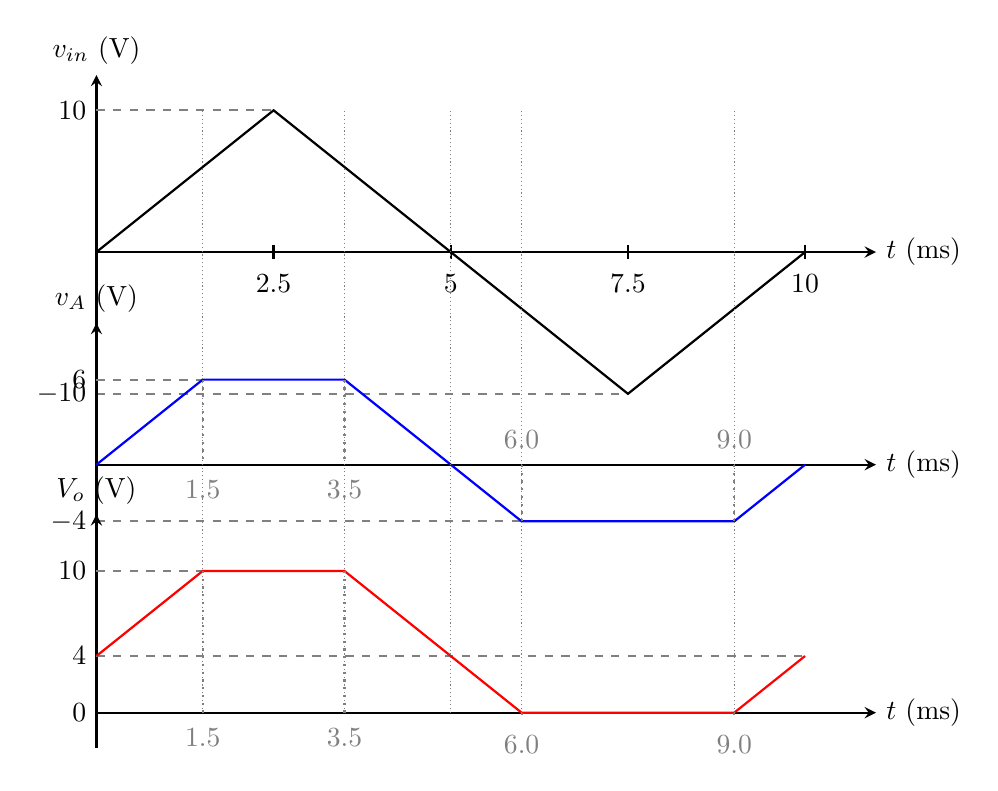
\begin{tikzpicture}[scale=0.9, >=stealth]
    % --- Plot 1: Input vin(t) ---
    \begin{scope}[yshift=6.5cm]
        \draw[->, thick] (0,0) -- (11,0) node[right] {$t$ (ms)};
        \draw[->, thick] (0,-2.5) -- (0,2.5) node[above] {$v_{in}$ (V)};
        
        \draw[gray, dashed] (0,2) -- (2.5,2);
        \draw[gray, dashed] (0,-2) -- (7.5,-2);
        \node[left] at (0,2) {$10$};
        \node[left] at (0,-2) {$-10$};
        
        \draw[thick] (0,0) -- (2.5,2) -- (5,0) -- (7.5,-2) -- (10,0);
        \foreach \x in {2.5, 5, 7.5, 10} \draw (\x, 0.1) -- (\x, -0.1) node[below=2pt] {\x};
    \end{scope}
    
    % --- Plot 2: Intermediate vA(t) ---
    \begin{scope}[yshift=3.5cm]
        \draw[->, thick] (0,0) -- (11,0) node[right] {$t$ (ms)};
        \draw[->, thick] (0,-1.5) -- (0,2.0) node[above] {$v_A$ (V)};
        
        \draw[gray, dashed] (0,1.2) -- (1.5,1.2);
        \draw[gray, dashed] (0,-0.8) -- (6,-0.8);
        \node[left] at (0,1.2) {$6$};
        \node[left] at (0,-0.8) {$-4$};
        
        \draw[blue, thick] (0,0) -- (1.5,1.2) -- (3.5,1.2) -- (5,0) -- (6,-0.8) -- (9,-0.8) -- (10,0);
        
        \draw[dotted, gray] (1.5, 1.2) -- (1.5, 0) node[below=2pt] {1.5};
        \draw[dotted, gray] (3.5, 1.2) -- (3.5, 0) node[below=2pt] {3.5};
        \draw[dotted, gray] (6, -0.8) -- (6, 0) node[above=2pt] {6.0};
        \draw[dotted, gray] (9, -0.8) -- (9, 0) node[above=2pt] {9.0};
    \end{scope}
    
    % --- Plot 3: Output Vo(t) ---
    \begin{scope}[yshift=0cm]
        \draw[->, thick] (0,0) -- (11,0) node[right] {$t$ (ms)};
        \draw[->, thick] (0,-0.5) -- (0,2.8) node[above] {$V_o$ (V)};
        
        \draw[gray, dashed] (0,2.0) -- (1.5,2.0);
        \draw[gray, dashed] (0,0.8) -- (10,0.8);
        \node[left] at (0,2.0) {$10$};
        \node[left] at (0,0.8) {$4$};
        \node[left] at (0,0) {$0$};
        
        \draw[red, thick] (0,0.8) -- (1.5,2.0) -- (3.5,2.0) -- (5,0.8) -- (6,0) -- (9,0) -- (10,0.8);
        
        \draw[dotted, gray] (1.5, 2.0) -- (1.5, 0) node[below=2pt] {1.5};
        \draw[dotted, gray] (3.5, 2.0) -- (3.5, 0) node[below=2pt] {3.5};
        \draw[dotted, gray] (6, 0) -- (6, -0.1) node[below=2pt] {6.0};
        \draw[dotted, gray] (9, 0) -- (9, -0.1) node[below=2pt] {9.0};
    \end{scope}
    
    % Vertical alignment guidlines connecting all three plots
    \foreach \x in {1.5, 3.5, 5, 6, 9} {
        \draw[gray, thin, densely dotted] (\x, 0) -- (\x, 8.5);
    }
\end{tikzpicture}
\end{center}

\end{tcolorbox}

\item Sketch the output waveform and transfer characteristics for the circuit shown. Assume the diode is ideal and $V_s$ is a sinusoid with 5\,V peak amplitude and frequency 5\,kHz.

\begin{center}
\begin{circuitikz}[thick,american, thick, scale=1.2, transform shape]
  
  % Left branch: Voltage source v_s
  \draw (0,3) to[V, l=$v_s$] (0,0);
  
  % Top branch: Resistor R
  \draw (0,3) to[R, l=$R$] (3,3);
  
  % Right branch: Diode and 2V Battery
  % D is the diode pointing down
  % battery1 represents the DC source. The longer line is positive.
  \draw (3,3) to[D] (3,1.5);
  \draw (3,0) to[battery1, l_=$2\text{ V}$] (3,1.5);
        
  % Bottom wire closing the loop
  \draw (3,0) -- (0,0);
  
  % Output terminals for v_0
  \draw (3,3) to[short, *-o] (4.5,3) node[below] {$+$};
  \draw (3,0) to[short, *-o] (4.5,0) node[above] {$-$};
  
  % Output voltage label v_0
  \node at (4.5, 1.5) {$v_0$};


\end{circuitikz}
\end{center}

\mk{15} \yr{EEE 263 | L-2/T-1 | 2011--12}

\begin{tcolorbox}[enhanced,breakable,ansbox,colback=cA!4,colframe=cA,boxrule=0.8pt,arc=5pt,title={\textbf{Answer}},fonttitle=\bfseries\color{white},colbacktitle=cA]

\subsection*{1. Circuit Analysis and Operating Regions}
The given circuit is a \textbf{positive clipper}. The diode's cathode is connected to the positive terminal of a $2\text{ V}$ DC source, holding it at a potential of $+2\text{ V}$. We are instructed to assume an \textbf{ideal diode}, meaning the forward voltage drop is $0\text{ V}$ ($V_\gamma = 0$).

The input voltage is a sinusoid: $v_s(t) = 5\sin(2\pi f t)$, with a peak amplitude of $5\text{ V}$ and a frequency of $f = 5\text{ kHz}$.
The time period of the signal is $T = \frac{1}{f} = \frac{1}{5000} = 0.2\text{ ms}$.

We can determine the circuit's behavior by analyzing the states of the diode:
\begin{itemize}
    \item \textbf{Region I: Diode OFF ($v_s < 2\text{ V}$)}
    When the input voltage is less than $2\text{ V}$, the potential at the anode is lower than the potential at the cathode. The diode is reverse-biased and acts as an open circuit. Since no current flows through resistor $R$, there is no voltage drop across it.
    \begin{equation}
        v_0 = v_s
    \end{equation}
    
    \item \textbf{Region II: Diode ON ($v_s \ge 2\text{ V}$)}
    When the input voltage reaches or exceeds $2\text{ V}$, the diode becomes forward-biased. As an ideal diode, it acts as a short circuit. The output voltage is directly clamped to the DC battery voltage.
    \begin{equation}
        v_0 = 2\text{ V}
    \end{equation}
\end{itemize}

\vspace{0.5cm}

\subsection*{2. Voltage Transfer Characteristics (VTC)}
The transfer characteristic relates the output $v_0$ to the input $v_s$. It has a linear slope of $1$ for $v_s < 2\text{ V}$ and a horizontal slope of $0$ for $v_s \ge 2\text{ V}$.

\begin{center}
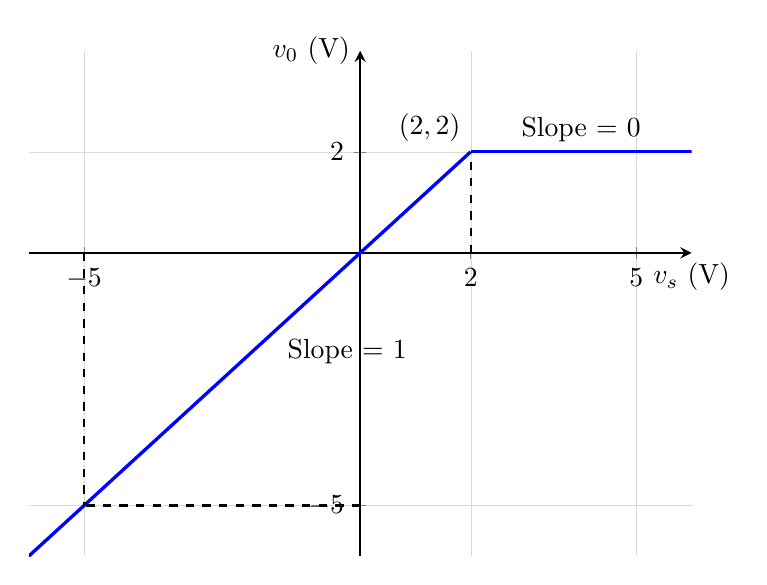
\begin{tikzpicture}
    \begin{axis}[
        width=10cm, height=8cm,
        xmin=-6, xmax=6,
        ymin=-6, ymax=4,
        axis lines=center,
        xlabel={$v_s$ (V)},
        ylabel={$v_0$ (V)},
        xtick={-5, 2, 5},
        ytick={-5, 2},
        grid=both,
        grid style={line width=.1pt, draw=gray!30},
        axis line style={thick},
        tick label style={font=\normalsize},
        xlabel style={anchor=north},
        ylabel style={anchor=east}
    ]
        
    % Transfer Curve
    \addplot[blue, very thick, domain=-6:2, samples=100] {x};
    \addplot[blue, very thick, domain=2:6, samples=100] {2};
    
    % Dashed projection lines
    \draw[dashed, black, thick] (axis cs:2,0) -- (axis cs:2,2);
    \draw[dashed, black, thick] (axis cs:-5,0) -- (axis cs:-5,-5);
    \draw[dashed, black, thick] (axis cs:0,-5) -- (axis cs:-5,-5);

    % Labels
    \node[anchor=south east] at (axis cs: 2, 2) {$(2, 2)$};
    \node[anchor=north west] at (axis cs: -1.5, -1.5) {Slope = $1$};
    \node[anchor=south] at (axis cs: 4, 2) {Slope = $0$};
    
    \end{axis}
\end{tikzpicture}
\end{center}

\vspace{0.5cm}

\subsection*{3. Output Waveform Sketch}
The input $v_s$ is a $5\text{ V}$ peak sine wave with a period of $0.2\text{ ms}$. The output perfectly tracks the input for all voltages below $2\text{ V}$ and clips exactly at $+2\text{ V}$ during the positive half-cycles.

\begin{center}
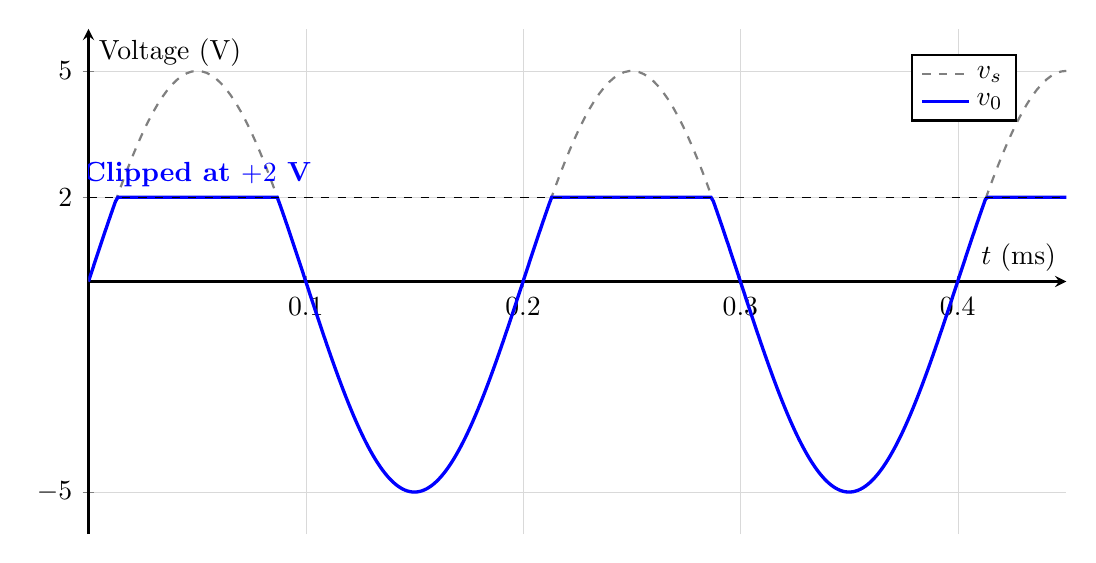
\begin{tikzpicture}
    \begin{axis}[
        width=14cm, height=8cm,
        xmin=0, xmax=0.45,
        ymin=-6, ymax=6,
        axis lines=center,
        xlabel={$t$ (ms)},
        ylabel={Voltage (V)},
        xtick={0.1, 0.2, 0.3, 0.4},
        ytick={-5, 2, 5},
        grid=both,
        grid style={line width=.1pt, draw=gray!30},
        axis line style={thick},
        tick label style={font=\normalsize},
        legend style={at={(0.95,0.95)},anchor=north east},
        declare function={
            vs(\t) = 5*sin(360 * \t / 0.2);
            v0(\t) = vs(\t) > 2 ? 2 : vs(\t);
        }
    ]
        
    % Input Waveform
    \addplot[dashed, gray, thick, domain=0:0.45, samples=200] {vs(x)};
    \addlegendentry{$v_s$}
    
    % Output Waveform
    \addplot[blue, very thick, domain=0:0.45, samples=400] {v0(x)};
    \addlegendentry{$v_0$}

    % Annotations for clipping point
    \draw[dashed, black, thin] (axis cs: 0, 2) -- (axis cs: 0.45, 2);
    
    \node[anchor=south, text=blue] at (axis cs: 0.05, 2) {\textbf{Clipped at $+2\text{ V}$}};

    \end{axis}
\end{tikzpicture}
\end{center}

\end{tcolorbox}


\end{enumerate}

%%──────────────────────────────────────────────────────────────────────
\subtopic{cA}{Clamping Circuits}
\label{sub:s2-clamping}

\begin{enumerate}
    
\item Design a clamper circuit to perform the function indicated in the figure (input $v_i$, output $v_0$). Assume ideal diodes.
\begin{center}
        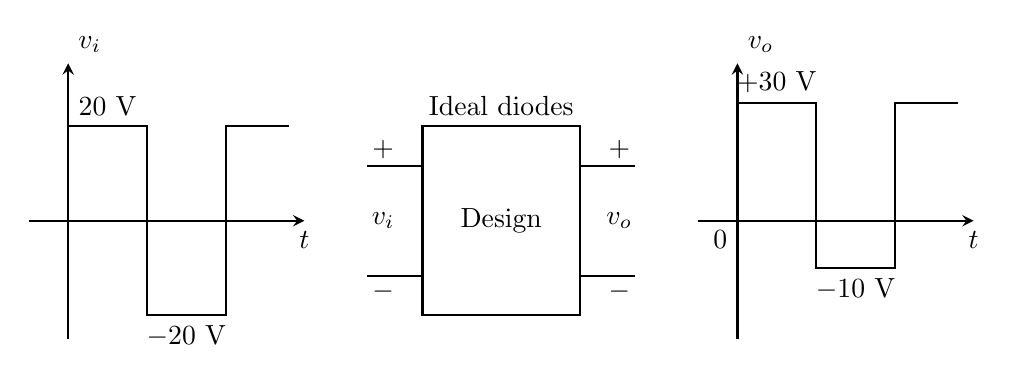
\begin{tikzpicture}[scale=1.0, >=stealth]
        
        % ==========================================
        % LEFT GRAPH: Input Waveform (v_i)
        % ==========================================
        % Axes
        \draw[->] (-0.5, 0) -- (3, 0) node[below] {$t$};
        \draw[->] (0, -1.5) -- (0, 2) node[above right] {$v_i$};
        
        % Waveform (+20V to -20V)
        \draw[thick] (0, 1.2) -- (1, 1.2) -- (1, -1.2) -- (2, -1.2) -- (2, 1.2) -- (2.8, 1.2);
        
        % Waveform Labels
        \node[above] at (0.5, 1.2) {$20\text{ V}$};
        \node[below] at (1.5, -1.2) {$-20\text{ V}$};
        
        % ==========================================
        % MIDDLE DIAGRAM: Design Block
        % ==========================================
        % The Block Box
        \draw[thick] (4.5, -1.2) rectangle (6.5, 1.2);
        \node at (5.5, 0) {Design};
        \node[above] at (5.5, 1.2) {Ideal diodes};
        
        % Left Input Terminals
        \draw (3.8, 0.7) -- (4.5, 0.7);
        \draw (3.8, -0.7) -- (4.5, -0.7);
        \node at (4.0, 0.9) {$+$};
        \node at (4.0, -0.9) {$-$};
        \node at (4.0, 0) {$v_i$};
        
        % Right Output Terminals
        \draw (6.5, 0.7) -- (7.2, 0.7);
        \draw (6.5, -0.7) -- (7.2, -0.7);
        \node at (7.0, 0.9) {$+$};
        \node at (7.0, -0.9) {$-$};
        \node at (7.0, 0) {$v_o$};
        
        % ==========================================
        % RIGHT GRAPH: Output Waveform (v_o)
        % ==========================================
        % Axes
        \draw[->] (8, 0) -- (11.5, 0) node[below] {$t$};
        \draw[->] (8.5, -1.5) -- (8.5, 2) node[above right] {$v_o$};
        \node[below left] at (8.5, 0) {$0$};
        
        % Waveform (+30V to -10V)
        \draw[thick] (8.5, 1.5) -- (9.5, 1.5) -- (9.5, -0.6) -- (10.5, -0.6) -- (10.5, 1.5) -- (11.3, 1.5);
        
        % Waveform Labels
        \node[above] at (9, 1.5) {$+30\text{ V}$};
        \node[below] at (10, -0.6) {$-10\text{ V}$};
        
        
    \end{tikzpicture}
\end{center}
\mk{12} \yr{EEE 263 | L-2/T-1 | 2022--23}

\begin{tcolorbox}[enhanced,breakable,ansbox,colback=cA!4,colframe=cA,boxrule=0.8pt,arc=5pt,title={\textbf{Answer}},fonttitle=\bfseries\color{white},colbacktitle=cA]

\subsection*{1. Analyze the Waveforms}
To design the clamper circuit, we first compare the input and output waveforms to determine the required DC shift:
\begin{itemize}
    \item \textbf{Input Waveform ($v_i$):} Square wave alternating between $+20\text{ V}$ and $-20\text{ V}$. The peak-to-peak voltage is $40\text{ V}$.
    \item \textbf{Output Waveform ($v_o$):} Square wave alternating between $+30\text{ V}$ and $-10\text{ V}$. The peak-to-peak voltage is still $40\text{ V}$, confirming the circuit is a clamper (DC restorer).
\end{itemize}

The entire waveform has been shifted upwards. The amount of DC shift added to the signal is:
\begin{equation}
    V_{DC} = V_{max(out)} - V_{max(in)} = 30\text{ V} - 20\text{ V} = \mathbf{+10\text{ V}}
\end{equation}

\subsection*{2. Clamper Circuit Design}
Because the waveform is shifted upwards, we need a \textbf{positive clamper}. A positive clamper consists of a capacitor in series with the input and a diode in parallel pointing \textit{upwards}.

To determine the reference voltage for the diode:
\begin{itemize}
    \item During the negative half-cycle, $v_i = -20\text{ V}$. The output $v_o$ must be clamped to its minimum value of $-10\text{ V}$.
    \item For the upwards-pointing diode to turn ON and clamp the output at $-10\text{ V}$, its anode must be held at a $-10\text{ V}$ potential relative to ground. 
    \item This is achieved by connecting a $10\text{ V}$ DC source in series with the diode, with the negative terminal connected to the diode's anode and the positive terminal connected to ground.
\end{itemize}

\subsection*{3. Circuit Diagram}
\begin{center}
\begin{circuitikz}[thick, american, scale=1.3, transform shape]
    % Input terminals
    \draw (0,2) to[short, o-] (1,2);
    \draw (0,0) to[short, o-] (5,0);
    
    \node[left] at (0,2) {$+$};
    \node[left] at (0,0) {$-$};
    \node[left] at (0,1) {$v_i$};
    
    % Capacitor
    \draw (1,2) to[C, l=$C$] (3,2);
    
    % Diode and Battery Branch
    \draw (3,2) to[short, *-] (3,2); 
    \draw (3,0) to[battery1] (3,1);
    \draw (3,1) to[empty diode] (3,2);
    
    % Battery Labels explicitly for clarity
    \node at (2.5, 0.8) {$-$};
    \node at (2.5, 0.2) {$+$};
    \node[left] at (2.4, 0.5) {$10\text{ V}$};
    
    % Output terminals
    \draw (3,2) to[short, -o] (5,2);
    \draw (3,0) to[short, -o] (5,0);
    
    \node[right] at (5,2) {$+$};
    \node[right] at (5,0) {$-$};
    \node[right] at (5,1) {$v_o$};
\end{circuitikz}
\end{center}

\subsection*{4. Verification}
\begin{itemize}
    \item \textbf{Negative Half-Cycle ($v_i = -20\text{ V}$):} The diode is forward-biased and turns ON. The output $v_o$ is clamped directly to the battery voltage ($-10\text{ V}$). The capacitor $C$ charges to $+10\text{ V}$ (right plate positive relative to the left plate) via KVL: $-20 - V_C = -10 \implies V_C = -10\text{ V}$ (from left to right), so the right plate is $10\text{ V}$ higher.
    \item \textbf{Positive Half-Cycle ($v_i = +20\text{ V}$):} The diode is reverse-biased and turns OFF. The fully charged capacitor acts as a series $10\text{ V}$ battery. The output voltage becomes $v_o = v_i + V_{C(right)} = 20\text{ V} + 10\text{ V} = +30\text{ V}$. This perfectly matches the required output.
\end{itemize}

\end{tcolorbox}

\item For the following circuit, draw the output waveshape for the given square input waveshape.
\begin{center}
    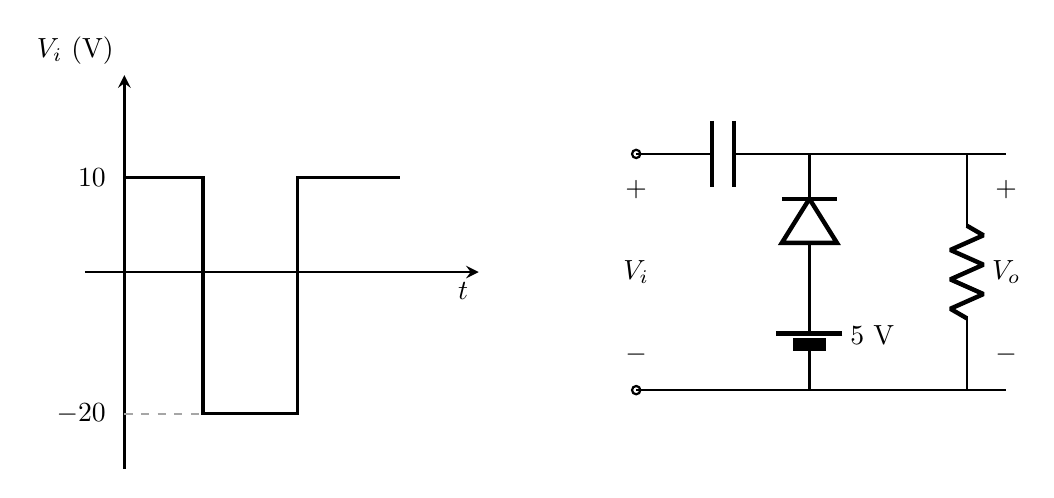
\begin{tikzpicture}[american, line width=0.8pt]

    % =========================================================================
    % LEFT SIDE: Input Waveform Graph (Vi vs t)
    % =========================================================================
    \begin{scope}[shift={(0,0)}]
        % Axes
        \draw[->, >=stealth, line width=1pt] (-0.5, 0) -- (4.5, 0) node[below left] {$t$};
        \draw[->, >=stealth, line width=1pt] (0, -2.5) -- (0, 2.5) node[above left] {$V_i\text{ (V)}$};

        % Square Waveform Path
        \draw[line width=1.2pt, color=black] 
            (0, 1.2) -- (1.0, 1.2) -- (1.0, -1.8) -- (2.2, -1.8) -- (2.2, 1.2) -- (3.5, 1.2);

        % Dashed helper line for negative peak
        \draw[dashed, color=gray!70] (0, -1.8) -- (1.0, -1.8);

        % Y-Axis Labels
        \node[left=3pt] at (0, 1.2) {$10$};
        \node[left=3pt] at (0, -1.8) {$-20$};
    \end{scope}


    % =========================================================================
    % RIGHT SIDE: Clamping Circuit Diagram
    % =========================================================================
    % Shifted to x=6.5 to give plenty of free drawing space and avoid overlap
    \begin{scope}[shift={(6.5,0)}]
        
        % Input Terminals
        \coordinate (in_top) at (0, 1.5);
        \coordinate (in_bot) at (0, -1.5);
        
        \draw (in_top) circle (1.5pt);
        \draw (in_bot) circle (1.5pt);
        
        % Input Voltage Label (+ Vi -)
        \draw (in_top) to[open, v=$V_i$] (in_bot);

        % Top wire through Capacitor
        \draw (in_top) to[C, name=C1] (2.2, 1.5) coordinate (junction_top);
        
        % Diode and DC Voltage Source Branch (Middle)
        % Diode points upwards, 5V Battery oriented with positive terminal up
        \draw (junction_top) to[diode, invert] (2.2, -0.2)
                            to[battery2, l=$5\text{ V}$] (2.2, -1.5) coordinate (junction_bot);

        % Parallel Resistor and Output Terminal Branch (Right)
        \draw (junction_top) -- (4.2, 1.5) coordinate (out_top)
              to[R, name=R1] (4.2, -1.5) coordinate (out_bot)
              -- (junction_bot);

        % Bottom Return Wire to Input
        \draw (junction_bot) -- (in_bot);

        % Output Voltage Label (+ Vo -)
        \draw (out_top) -- ++(0.5,0) coordinate (ext_top);
        \draw (out_bot) -- ++(0.5,0) coordinate (ext_bot);
        \draw (ext_top) to[open, v=$V_o$] (ext_bot);

    \end{scope}

    % =========================================================================
    % GLOBAL CAPTION
    % =========================================================================
\end{tikzpicture}
\end{center}
\mk{16} \yr{EEE 263 | L-2/T-1 | Jan 2021}

\begin{tcolorbox}[enhanced,breakable,ansbox,colback=cA!4,colframe=cA,boxrule=0.8pt,arc=5pt,title={\textbf{Answer}},fonttitle=\bfseries\color{white},colbacktitle=cA]

\subsection*{1. Circuit Identification and Reference Level}
The given circuit is a \textbf{positive clamper}. The diode points upwards, which means it will prevent the output voltage from dropping below a specific reference level, effectively shifting the entire waveform up. 

The reference voltage is determined by the DC source connected in series with the diode. The longer line of the battery symbol is on top, indicating its positive terminal is connected to the diode's anode. Thus, the reference clamping level is $+5\text{ V}$. Assuming an ideal diode, it will turn ON whenever the output tries to drop below 5 V.

\subsection*{2. Operation During the Negative Half-Cycle}
The clamper sets its DC shift during the cycle that forward-biases the diode.
\begin{itemize}
    \item When the input drops to $V_i = -20\text{ V}$, the output tries to swing negative. Because this potential is lower than the anode potential (5 V), the diode is forward-biased and acts as a short circuit.
    \item The output is directly clamped to the battery voltage:
    \begin{equation}
        V_o = 5\text{ V}
    \end{equation}
    \item During this time, the capacitor ($C$) charges. Applying Kirchhoff's Voltage Law (KVL) to the outer loop ($V_i - V_C - V_o = 0$):
    \begin{equation}
        -20\text{ V} - V_C - 5\text{ V} = 0 \implies V_C = -25\text{ V}
    \end{equation}
    This means the capacitor charges to 25 V, with its right plate positive relative to its left plate.
\end{itemize}

\subsection*{3. Operation During the Positive Half-Cycle}
\begin{itemize}
    \item When the input rises to $V_i = 10\text{ V}$, the cathode of the diode is pushed to a higher potential than the 5 V anode. The diode becomes reverse-biased and acts as an open circuit.
    \item The fully charged capacitor acts as a series 25 V battery. The output voltage is the sum of the input voltage and the capacitor voltage:
    \begin{equation}
        V_o = V_i + V_{C(\text{right plate})} = 10\text{ V} + 25\text{ V} = 35\text{ V}
    \end{equation}
\end{itemize}
\textit{Verification:} The peak-to-peak voltage of the input is $10\text{ V} - (-20\text{ V}) = 30\text{ V}$. The peak-to-peak voltage of the output is $35\text{ V} - 5\text{ V} = 30\text{ V}$. The amplitude is perfectly preserved, and the signal has been shifted upwards by 25 V.

\vspace{0.5cm}

\subsection*{4. Output Waveform Sketch}
The resulting steady-state output is a square wave that alternates between 35 V and 5 V, synchronized with the input waveform's timing.

\begin{center}
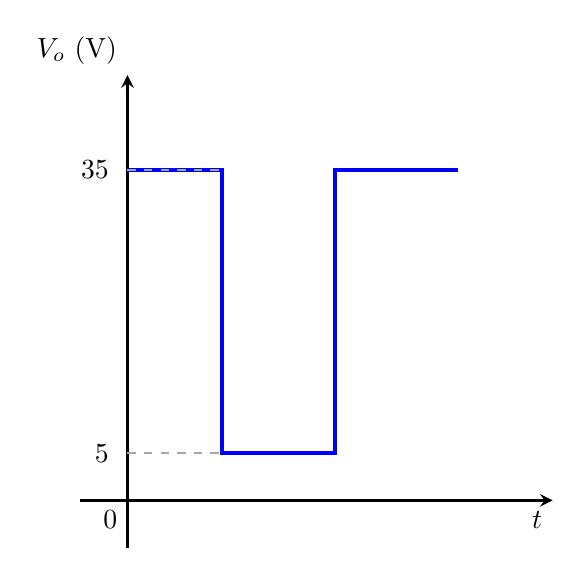
\begin{tikzpicture}[american, line width=0.8pt, scale=1.2]

    % Axes
    \draw[->, >=stealth, line width=1pt] (-0.5, 0) -- (4.5, 0) node[below left] {$t$};
    \draw[->, >=stealth, line width=1pt] (0, -0.5) -- (0, 4.5) node[above left] {$V_o\text{ (V)}$};

    % Square Waveform Path (Scaling 10V = 1 unit for Y-axis)
    \draw[line width=1.5pt, color=blue] 
        (0, 3.5) -- (1.0, 3.5) -- (1.0, 0.5) -- (2.2, 0.5) -- (2.2, 3.5) -- (3.5, 3.5);

    % Dashed helper lines
    \draw[dashed, color=gray!70] (0, 3.5) -- (1.0, 3.5);
    \draw[dashed, color=gray!70] (0, 0.5) -- (1.0, 0.5);

    % Y-Axis Labels
    \node[left=3pt] at (0, 3.5) {\textbf{$35$}};
    \node[left=3pt] at (0, 0.5) {\textbf{$5$}};
    \node[below left] at (0, 0) {$0$};

\end{tikzpicture}
\end{center}

\end{tcolorbox}

\item For the circuit shown, neatly draw the output waveform ($v_o$) corresponding to the input waveform ($v_{in}$) in steady state. Assume the diode is non-ideal.
\begin{center}
  
    \begin{circuitikz}[thick,scale=1.1, transform shape]
        
        % ==========================================
        % বাম দিকের অংশ: Input Graph (Square Wave)
        % ==========================================
        \begin{scope}[shift={(0,0)}]
            % Axes (অক্ষ)
            \draw[->, thick] (0,-1.8) -- (0,1.8) node[above] {$v_{in}$};
            \draw[->, thick] (0,0) -- (3.5,0) node[right] {$t$};
            
            % Square Wave (স্কয়ার ওয়েভ)
            \draw[thick] (0,1.2) -- (0.8,1.2) -- (0.8,-1.2) -- (1.6,-1.2) -- (1.6,1.2) -- (2.4,1.2) -- (2.4,-1.2) -- (3.2,-1.2);
            
            % Y-axis labels (ভোল্টেজ লেবেল)
            \node[left] at (0,1.2) {$+5\mathrm{V}$};
            \node[left] at (0,-1.2) {$-5\mathrm{V}$};
            
            % Dotted lines and Time label (সময় লেবেল)
            \draw[dashed] (0,-1.2) -- (0.8,-1.2);
            \draw[dashed] (1.6,0) -- (1.6,-1.5);
            \node[below] at (1.6, -1.5) {$1\mathrm{ms}$};
        \end{scope}
        
        % ==========================================
        % ডান দিকের অংশ: Diode Circuit
        % ==========================================
        \begin{scope}[shift={(5,-1)}]
            % 1. Square Wave Voltage Source
            \draw (0,0) to[sqV] (0,2.4);
            \node[left] at (-0.4, 2.4) {$+$};
            \node[left] at (-0.6, 1.2) {$v_{in}$};
            \node[left] at (-0.4, 0) {$-$};
            
            % 2. Top Branch (Series Resistor & Capacitor)
            \draw (0,2.4) to[R, l={$1\mathrm{K}$}] (2,2.4) to[C, l={$10\mu\mathrm{F}$}] (4.5,2.4);
            
            % 3. Parallel Branches (Diode & Resistor)
            \draw (4.5,0) to[empty diode] (4.5,2.4); % Diode pointing upwards
            \draw (6.5,0) to[R, l={$2\mathrm{K}$}] (6.5,2.4); % Parallel Resistor
            
            % 4. Connections & Bottom Wire
            \draw (4.5,2.4) -- (6.5,2.4);
            \draw (0,0) -- (6.5,0);
            
            % 5. Junction Dots
            \fill (4.5,2.4) circle (1.5pt);
            \fill (4.5,0) circle (1.5pt);
            \fill (6.5,2.4) circle (1.5pt);
            \fill (6.5,0) circle (1.5pt);
            
            % 6. Output Terminals
            \draw (6.5,2.4) to[short, -o] (8,2.4);
            \draw (6.5,0) to[short, -o] (8,0);
            
            \node[right] at (8.1, 2.4) {$+$};
            \node[right] at (8.1, 1.2) {$v_o$};
            \node[right] at (8.1, 0) {$-$};
            
        \end{scope}
        
    \end{circuitikz}
\end{center}
\mk{15} \yr{EEE 263 | L-2/T-1 | 2015--16}

\begin{tcolorbox}[enhanced,breakable,ansbox,colback=cA!4,colframe=cA,boxrule=0.8pt,arc=5pt,title={\textbf{Answer}},fonttitle=\bfseries\color{white},colbacktitle=cA]

\subsection*{1. Circuit Analysis and Assumptions}
The given circuit is a clamper circuit with a non-ideal diode, a series resistor $R_1$, and a parallel load resistor $R_2$. To analyze the steady-state response, we make the following assumptions:
\begin{itemize}
    \item \textbf{Non-ideal Diode Model:} We assume a constant voltage drop (CVD) model for the silicon diode, where the forward voltage drop is $V_\gamma = 0.7\text{ V}$ and the forward resistance is $r_f = 0\ \Omega$.
    \item \textbf{Steady-State Operation:} The input square wave has a frequency of $f = 1\text{ kHz}$ (since $T = 1\text{ ms}$). The half-period is $T/2 = 0.5\text{ ms}$.
    \item \textbf{Time Constants:} 
    \begin{itemize}
        \item When the diode is ON, the equivalent resistance charging the capacitor is $R_{eq,ON} \approx R_1 = 1\text{ k}\Omega$. The charging time constant is $\tau_{ON} = R_1 C = 1\text{ k}\Omega \times 10\mu\text{F} = 10\text{ ms}$.
        \item When the diode is OFF, the equivalent resistance is $R_{eq,OFF} = R_1 + R_2 = 3\text{ k}\Omega$. The discharging time constant is $\tau_{OFF} = (R_1 + R_2) C = 3\text{ k}\Omega \times 10\mu\text{F} = 30\text{ ms}$.
    \end{itemize}
    Since both $\tau_{ON} = 10\text{ ms} \gg 0.5\text{ ms}$ and $\tau_{OFF} = 30\text{ ms} \gg 0.5\text{ ms}$, the capacitor does not have enough time to significantly charge or discharge during a single half-cycle. Therefore, we can assume the voltage across the capacitor, $V_C$, remains approximately constant in steady state.
\end{itemize}

Let $V_C$ be the steady-state DC voltage across the capacitor, defined with the positive terminal on the left plate. 

\subsection*{2. Circuit States and Operating Regions}
We analyze the two distinct states corresponding to the two half-cycles of the input waveform.

\textbf{State 1: Positive Half-Cycle ($0 \le t < 0.5\text{ ms}$)}
During this interval, $v_{in} = +5\text{ V}$. 
The positive input reverse-biases the upward-pointing diode (Diode OFF). The circuit simplifies to a voltage divider consisting of $v_{in}$, $R_1$, $C$, and $R_2$ in series.
The loop current $i_1$ (flowing left to right) is:
\begin{equation}
    i_1 = \frac{v_{in} - V_C}{R_1 + R_2} = \frac{5 - V_C}{1\text{ k}\Omega + 2\text{ k}\Omega} = \frac{5 - V_C}{3\text{ k}\Omega}
\end{equation}
The output voltage $v_{o1}$ across $R_2$ is:
\begin{equation}
    v_{o1} = i_1 R_2 = \left( \frac{5 - V_C}{3\text{ k}\Omega} \right) \times 2\text{ k}\Omega = \frac{2}{3}(5 - V_C) \label{eq:vo1}
\end{equation}

\textbf{State 2: Negative Half-Cycle ($0.5\text{ ms} \le t < 1.0\text{ ms}$)}
During this interval, $v_{in} = -5\text{ V}$. 
The negative input pulls the cathode of the diode to a lower potential than its grounded anode, forward-biasing the diode (Diode ON). The output voltage is clamped to the negative diode drop:
\begin{equation}
    v_{o2} = -0.7\text{ V} \label{eq:vo2}
\end{equation}
The current $i_2$ flowing through the capacitor (left to right) is determined by the voltage drop across $R_1$:
\begin{equation}
    i_2 = \frac{v_{in} - V_C - v_{o2}}{R_1} = \frac{-5 - V_C - (-0.7)}{1\text{ k}\Omega} = \frac{-4.3 - V_C}{1\text{ k}\Omega}
\end{equation}

\subsection*{3. Steady-State Charge Balance}
In steady state, the net charge accumulating on the capacitor over one full period must be zero. This implies the average capacitor current is zero:
\begin{equation}
    i_1 \cdot \frac{T}{2} + i_2 \cdot \frac{T}{2} = 0 \implies i_1 + i_2 = 0
\end{equation}
Substituting the expressions for $i_1$ and $i_2$:
\begin{align*}
    \frac{5 - V_C}{3} + \frac{-4.3 - V_C}{1} &= 0 \notag \\
    (5 - V_C) + 3(-4.3 - V_C) &= 0 \notag \\
    5 - V_C - 12.9 - 3V_C &= 0 \notag \\
    -4V_C &= 7.9 \notag \\
    V_C &= -1.975\text{ V}
\end{align*}
The negative sign indicates that the right plate of the capacitor is actually at a higher potential than the left plate by $1.975\text{ V}$.

\subsection*{4. Final Output Voltages and Verification}
Using the calculated steady-state capacitor voltage $V_C = -1.975\text{ V}$:

\begin{itemize}
    \item \textbf{During the Positive Half-Cycle:}
    From Equation \eqref{eq:vo1}, the output voltage is:
    \begin{equation}
        v_{o1} = \frac{2}{3}(5 - (-1.975)) = \frac{2}{3}(6.975) = \mathbf{4.65\text{ V}}
    \end{equation}
    \textit{Verification:} Since $v_{o1} = 4.65\text{ V} > -0.7\text{ V}$, the diode is indeed reverse-biased, confirming our assumption.
    
    \item \textbf{During the Negative Half-Cycle:}
    From Equation \eqref{eq:vo2}, the output voltage is:
    \begin{equation}
        v_{o2} = \mathbf{-0.7\text{ V}}
    \end{equation}
    \textit{Verification:} Let's check if the diode current $I_D$ is positive (flowing upwards from ground). By applying KCL at the output node:
    \begin{align*}
        I_D &= i_{R2} - i_2 \\
        i_{R2} &= \frac{v_{o2}}{R_2} = \frac{-0.7\text{ V}}{2\text{ k}\Omega} = -0.35\text{ mA} \\
        i_2 &= \frac{-4.3 - (-1.975)}{1\text{ k}\Omega} = -2.325\text{ mA} \\
        I_D &= -0.35\text{ mA} - (-2.325\text{ mA}) = \mathbf{1.975\text{ mA}}
    \end{align*}
    Since $I_D > 0$, the diode is indeed forward-biased and conducting, validating our assumption.
\end{itemize}

\vspace{0.5cm}
\subsection*{5. Circuit Diagram and Output Waveform}

\begin{center}
    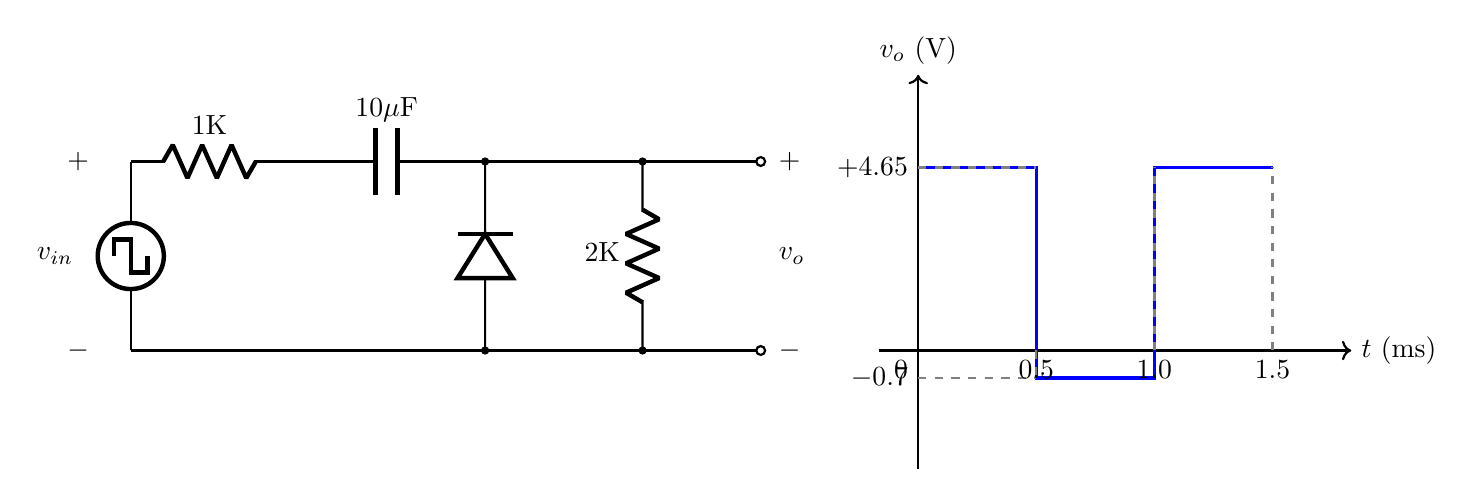
\begin{tikzpicture}[scale=1.0, transform shape]
        
        % ==========================================
        % LEFT SIDE: Original Circuit Redrawn
        % ==========================================
        \begin{scope}[shift={(0,0)}]
            % 1. Square Wave Voltage Source
            \draw (0,0) to[sqV] (0,2.4);
            \node[left] at (-0.4, 2.4) {$+$};
            \node[left] at (-0.6, 1.2) {$v_{in}$};
            \node[left] at (-0.4, 0) {$-$};
            
            % 2. Top Branch (Series Resistor & Capacitor)
            \draw (0,2.4) to[R, l={$1\mathrm{K}$}] (2,2.4) to[C, l={$10\mu\mathrm{F}$}] (4.5,2.4);
            
            % 3. Parallel Branches (Diode & Resistor)
            \draw (4.5,0) to[empty diode] (4.5,2.4); % Diode pointing upwards
            \draw (6.5,0) to[R, l={$2\mathrm{K}$}] (6.5,2.4); % Parallel Resistor
            
            % 4. Connections & Bottom Wire
            \draw (4.5,2.4) -- (6.5,2.4);
            \draw (0,0) -- (6.5,0);
            
            % 5. Junction Dots
            \fill (4.5,2.4) circle (1.5pt);
            \fill (4.5,0) circle (1.5pt);
            \fill (6.5,2.4) circle (1.5pt);
            \fill (6.5,0) circle (1.5pt);
            
            % 6. Output Terminals
            \draw (6.5,2.4) to[short, -o] (8,2.4);
            \draw (6.5,0) to[short, -o] (8,0);
            
            \node[right] at (8.1, 2.4) {$+$};
            \node[right] at (8.1, 1.2) {$v_o$};
            \node[right] at (8.1, 0) {$-$};
            
        \end{scope}

        % ==========================================
        % RIGHT SIDE: Steady-State Output Waveform
        % ==========================================
        \begin{scope}[shift={(10,0)}]
            % Axes
            \draw[->, thick] (-0.5, 0) -- (5.5, 0) node[right] {$t\text{ (ms)}$};
            \draw[->, thick] (0, -1.5) -- (0, 3.5) node[above] {$v_o\text{ (V)}$};
            
            % Output Square Wave (Scaled for visual clarity)
            \draw[blue, very thick] (0, 2.325) -- (1.5, 2.325) -- (1.5, -0.35) -- (3.0, -0.35) -- (3.0, 2.325) -- (4.5, 2.325);
            
            % Dashed guidelines and Time labels
            \draw[dashed, gray] (1.5,0) -- (1.5,-0.35);
            \draw[dashed, gray] (3.0,0) -- (3.0,2.325);
            \draw[dashed, gray] (4.5,0) -- (4.5,2.325);
            
            \draw[dashed, gray] (0, 2.325) -- (1.5, 2.325);
            \draw[dashed, gray] (0, -0.35) -- (1.5, -0.35);
            
            % Y-axis labels
            \node[left] at (0, 2.325) {$+4.65$};
            \node[left] at (0, -0.35) {$-0.7$};
            \node[below left] at (0, 0) {$0$};
            
            % X-axis labels
            \node[below] at (1.5, 0) {$0.5$};
            \node[below] at (3.0, 0) {$1.0$};
            \node[below] at (4.5, 0) {$1.5$};
        \end{scope}
        
    \end{tikzpicture}
\end{center}

\end{tcolorbox}


\item Draw the output wave shape ($v_0$) and also the $V_L$--$V_o$ graph for the circuit shown. Assume a constant 0.7\,V forward voltage drop across the diode.
\begin{center}
  
    \begin{circuitikz}[thick,scale=1.2, transform shape]

        % ===================================================
        % Left Side: AC Voltage Source
        % ===================================================
        % Notice the extra { } around the label to prevent the "=" sign error
        \draw (0,0) to[sinusoidal voltage source, l={$v_i = 3\sin(\omega t)$}] (0, 2.5);

        % ===================================================
        % Top Side: Curved Capacitor
        % ===================================================
        \draw (0, 2.5) -- (0.5, 2.5) coordinate (c_left);
        \draw (c_left) to[cC] (2.5, 2.5) coordinate (c_right);
        \draw (c_right) -- (3, 2.5);

        % ===================================================
        % Output Terminals (v0)
        % ===================================================
        \draw (c_left) -- ++(0, 0.5) node[draw, fill=white, minimum size=3.5pt, inner sep=0pt] {};
        \draw (c_right) -- ++(0, 0.5) node[draw, fill=white, minimum size=3.5pt, inner sep=0pt] {};
        
        \node[above] at (1.5, 2.9) {$+ \quad v_0 \quad -$};

        % ===================================================
        % Right Side: Diode and Battery (1v)
        % ===================================================
        \draw (3, 2.5) to[D] (3, 1.25);
        \draw (3, 1.25) to[battery1, l={$1\text{v}$}] (3, 0);

        % ===================================================
        % Bottom Side: Return Wire
        % ===================================================
        \draw (3, 0) -- (0, 0);

    \end{circuitikz}
\end{center}
\mk{20} \yr{EEE 263 | L-2/T-1 | 2013--14}

\begin{tcolorbox}[enhanced,breakable,ansbox,colback=cA!4,colframe=cA,boxrule=0.8pt,arc=5pt,title={\textbf{Answer}},fonttitle=\bfseries\color{white},colbacktitle=cA]

\subsection*{1. Circuit Analysis and Assumptions}
Based on the provided circuit diagram, the output voltage $v_0$ is explicitly defined as the voltage \textit{across the series capacitor} $C$, with the positive terminal on the left plate. We analyze the circuit with the following assumptions:
\begin{itemize}
    \item \textbf{Input Voltage:} The source is an AC sinusoidal voltage $v_i(t) = 3\sin(\omega t)$, with a peak amplitude of $V_m = 3\text{ V}$.
    \item \textbf{Diode Model:} We assume a Constant Voltage Drop (CVD) model for the diode, with a forward voltage of $V_\gamma = 0.7\text{ V}$.
    \item \textbf{DC Bias:} A $1\text{ V}$ DC battery is in series with the diode. Because the longer parallel line (positive terminal) is at the top, the cathode potential is $V_K = 1\text{ V}$ relative to ground.
    \item \textbf{Initial Condition:} The capacitor is initially uncharged, meaning $v_0(0) = 0\text{ V}$.
\end{itemize}

\subsection*{2. Mathematical Derivation}
The circuit consists of a single loop for charging the capacitor. The diode $D$ will turn ON (forward-biased) only when the potential at its anode ($V_A$) exceeds the potential at its cathode ($V_K$) by at least $V_\gamma$.

\textbf{Condition for Diode Conduction:}
\begin{align*}
    V_A - V_K &\ge V_\gamma \notag \\
    (v_i - v_0) - 1\text{ V} &\ge 0.7\text{ V} \notag \\
    v_i - v_0 &\ge 1.7\text{ V} \label{eq:cond}
\end{align*}

\textbf{Transient Charging Phase:}
\begin{itemize}
    \item Starting from $t=0$, as $v_i$ rises from $0\text{ V}$, the condition $v_i - v_0 \ge 1.7\text{ V}$ is not met initially. The diode remains OFF, no current flows, and $v_0 = 0\text{ V}$.
    \item When $v_i$ reaches $1.7\text{ V}$, the diode turns ON. For any further increase in $v_i$, applying Kirchhoff's Voltage Law (KVL) yields:
    \begin{equation}
        v_i - v_0 - 0.7\text{ V} - 1\text{ V} = 0 \implies v_0 = v_i - 1.7\text{ V}
    \end{equation}
    \item The input voltage $v_i$ reaches its maximum positive peak of $3\text{ V}$ at $t = T/4$. At this instant, the capacitor charges to its maximum voltage:
    \begin{equation}
        v_{0(\max)} = 3\text{ V} - 1.7\text{ V} = \mathbf{1.3\text{ V}}
    \end{equation}
\end{itemize}

\textbf{Steady-State Operation:}
\begin{itemize}
    \item After $v_i$ passes its positive peak and decreases, the quantity $(v_i - v_0)$ drops below $1.7\text{ V}$. The diode becomes reverse-biased and turns OFF.
    \item Because the diode is OFF and there is no parallel discharge path (ideal assumption), the capacitor perfectly retains its accumulated charge.
    \item Therefore, in steady state, the output voltage $v_0$ remains a constant DC value:
    \begin{equation}
        v_0(t) = \mathbf{1.3\text{ V}}
    \end{equation}
\end{itemize}

\vspace{0.5cm}
\subsection*{3. Circuit Diagram Redrawn}
\begin{center}
    \begin{circuitikz}[thick,scale=1.1, transform shape]
        % Input source
        \draw (0,0) to[sinusoidal voltage source, l={$v_i = 3\sin(\omega t)$}] (0, 2.5);
        
        % Top branch and Capacitor
        \draw (0, 2.5) -- (1, 2.5) coordinate (c_left);
        \draw (c_left) to[cC, l=$C$] (3, 2.5) coordinate (c_right);
        \draw (c_right) -- (4.5, 2.5);
        
        % Output terminals exactly across capacitor
        \draw (c_left) -- ++(0, 0.6) node[ocirc, fill=white] {};
        \draw (c_right) -- ++(0, 0.6) node[ocirc, fill=white] {};
        \node[above] at (2, 3.2) {$+ \quad v_0 \quad -$};
        
        % Diode and Battery branch
        \draw (4.5, 2.5) to[D, l=$D$, v=$V_\gamma {=} 0.7\text{V}$] (4.5, 1.25);
        \draw (4.5, 1.25) to[battery1, l={$1\text{ V}$}] (4.5, 0);
        
        % Return path
        \draw (4.5, 0) -- (0, 0);
    \end{circuitikz}
\end{center}

\vspace{0.5cm}
\subsection*{4. Output Waveforms and Transfer Characteristic}
\textit{Assumption: The requested "$V_L$" parameter denotes the line/input voltage $v_i$. The plots reflect the transient charging and the clamped steady-state behavior.}

\begin{center}
    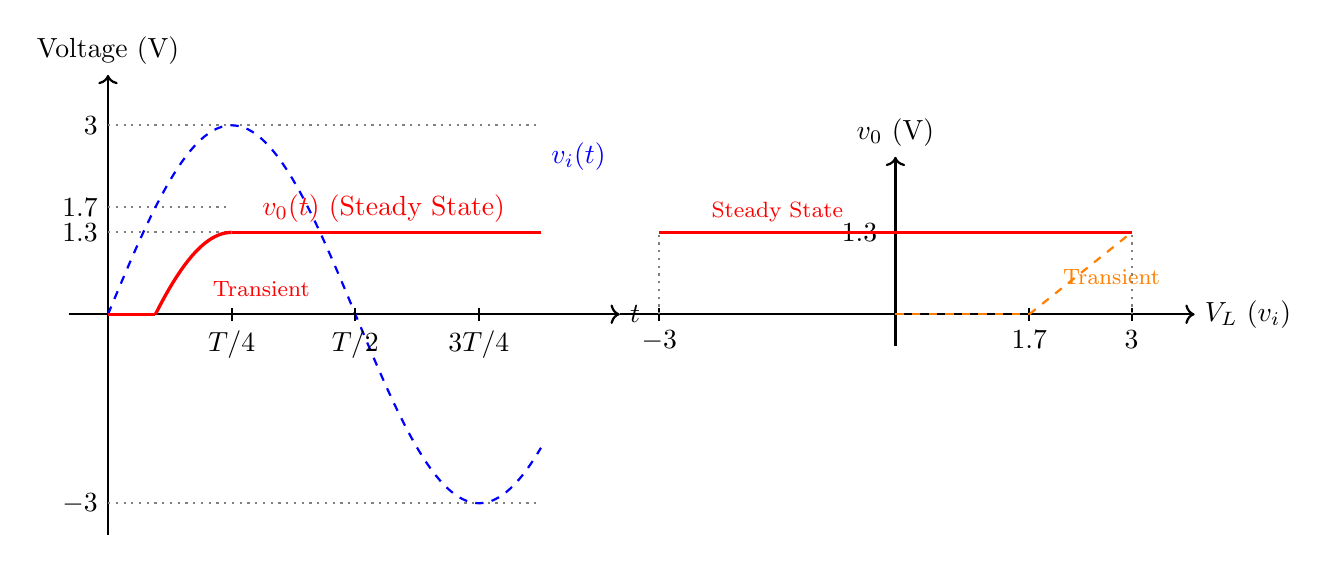
\begin{tikzpicture}[xscale=1.0, yscale=0.8]
        % ----------------------------------------------------
        % Left Graph: Waveforms (Time Domain)
        % ----------------------------------------------------
        \begin{scope}[shift={(0,0)}]
            \draw[->, thick] (-0.5, 0) -- (6.5, 0) node[right] {$t$};
            \draw[->, thick] (0, -3.5) -- (0, 3.8) node[above] {Voltage (V)};
            
            % Grid & Ticks
            \draw[dotted, gray] (0, 3) node[left, text=black] {$3$} -- (5.5, 3);
            \draw[dotted, gray] (0, -3) node[left, text=black] {$-3$} -- (5.5, -3);
            \draw[dotted, gray] (0, 1.7) node[left, text=black] {$1.7$} -- (1.57, 1.7);
            \draw[dotted, gray] (0, 1.3) node[left, text=black] {$1.3$} -- (5.5, 1.3);
            
            % v_i(t) Sine Wave
            \draw[dashed, blue, thick, domain=0:5.5, samples=100] plot (\x, {3*sin(\x r)});
            \node[blue, right] at (5.5, 2.5) {$v_i(t)$};
            
            % v_0(t) Output Wave
            % t1 = asin(1.7/3) approx 0.603
            % peak at pi/2 approx 1.57
            \draw[red, very thick] (0, 0) -- (0.603, 0);
            \draw[red, very thick, domain=0.603:1.57, samples=50] plot (\x, {3*sin(\x r) - 1.7});
            \draw[red, very thick] (1.57, 1.3) -- (5.5, 1.3);
            
            \node[red, above] at (3.5, 1.3) {$v_0(t)$ (Steady State)};
            \node[red, right] at (1.2, 0.4) {\footnotesize Transient};
            
            % Time labels
            \draw (1.57, 0.1) -- (1.57, -0.1) node[below] {$T/4$};
            \draw (3.14, 0.1) -- (3.14, -0.1) node[below] {$T/2$};
            \draw (4.71, 0.1) -- (4.71, -0.1) node[below] {$3T/4$};
        \end{scope}

        % ----------------------------------------------------
        % Right Graph: V_L - V_o Transfer Characteristic
        % ----------------------------------------------------
        \begin{scope}[shift={(10,0)}]
            \draw[->, thick] (-3.5, 0) -- (3.8, 0) node[right] {$V_L$ ($v_i$)};
            \draw[->, thick] (0, -0.5) -- (0, 2.5) node[above] {$v_0$ (V)};
            
            % Ticks
            \draw (3, 0.1) -- (3, -0.1) node[below] {$3$};
            \draw (-3, 0.1) -- (-3, -0.1) node[below] {$-3$};
            \draw (1.7, 0.1) -- (1.7, -0.1) node[below] {$1.7$};
            \draw (0.1, 1.3) -- (-0.1, 1.3) node[left] {$1.3$};
            
            % Transient Charging Path
            \draw[dashed, orange, thick] (0,0) -- (1.7, 0);
            \draw[dashed, orange, thick] (1.7, 0) -- (3, 1.3);
            \node[orange, right] at (2.0, 0.6) {\footnotesize Transient};
            
            % Steady State Path
            \draw[red, very thick] (-3, 1.3) -- (3, 1.3);
            \node[red, above] at (-1.5, 1.3) {\footnotesize Steady State};
            
            % Limit lines
            \draw[dotted, gray] (3, 0) -- (3, 1.3);
            \draw[dotted, gray] (-3, 0) -- (-3, 1.3);
        \end{scope}
    \end{tikzpicture}
\end{center}

\vspace{0.3cm}
\begin{tcolorbox}[colback=cA!10, colframe=cA!60, boxrule=0.5pt, title={\textbf{Important Note}}, fonttitle=\bfseries]
While the overall circuit functions as a positive clamper (where the load output is typically taken across the diode branch), the provided schematic \textbf{explicitly defines the output terminals ($v_0$) directly across the capacitor}. Therefore, the rigorous evaluation of $v_0$ yields the transient charging curve that resolves into a pure DC steady-state value of $1.3\text{V}$, rather than a shifted sinusoidal waveform.
\end{tcolorbox}

\end{tcolorbox}

\item Design a clamper circuit to perform the function indicated in the figure using an ideal diode.
\begin{center}
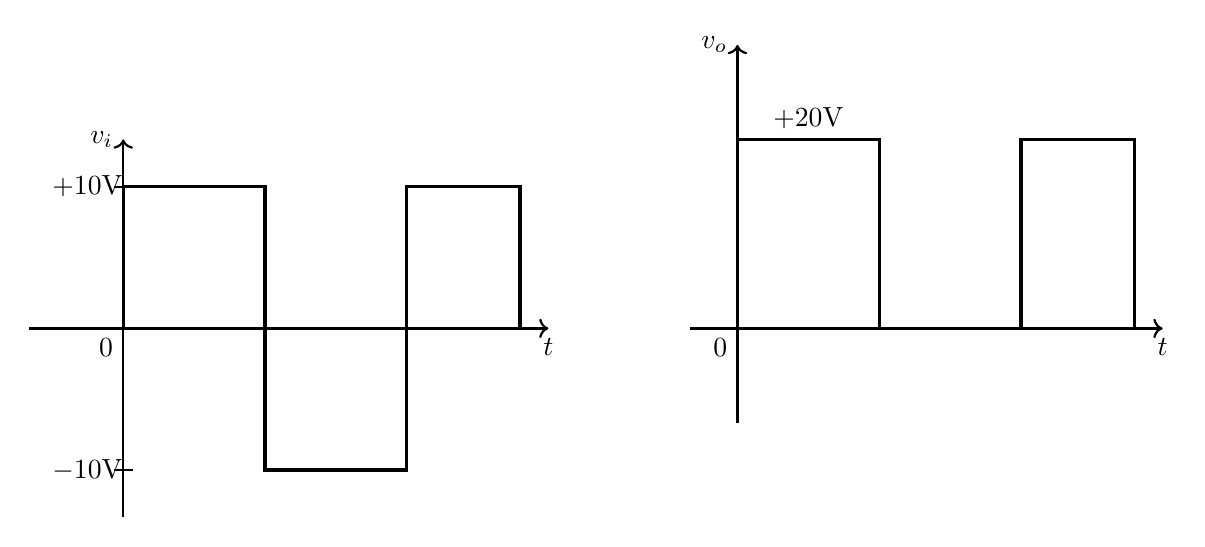
\begin{tikzpicture}[thick,scale=1.2]

  % ==========================================
  % বাম দিকের গ্রাফ: ইনপুট ভোল্টেজ (v_i)
  % ==========================================
  \begin{scope}[xshift=0cm]
    % X এবং Y অক্ষ (Axes)
    \draw[->, thick] (-1, 0) -- (4.5, 0) node[below] {$t$};
    \draw[->, thick] (0, -2) -- (0, 2) node[left] {$v_i$};
    
    % লেবেল এবং টিক মার্ক (Labels & Ticks)
    \node[below left] at (0,0) {0};
    \draw[thick] (-0.1, 1.5) -- (0.1, 1.5) node[left] {$+10\text{V}$};
    \draw[thick] (-0.1, -1.5) -- (0.1, -1.5) node[left] {$-10\text{V}$};
    
    % স্কয়ার ওয়েভ (Square Waveform)
    \draw[very thick] (0,0) -- (0,1.5) -- (1.5,1.5) -- (1.5,-1.5) -- (3,-1.5) -- (3,1.5) -- (4.2,1.5) -- (4.2,0);
  \end{scope}

  % ==========================================
  % ডান দিকের গ্রাফ: আউটপুট ভোল্টেজ (v_o) (Clamped Wave)
  % ==========================================
  \begin{scope}[xshift=6.5cm]
    % X এবং Y অক্ষ (Axes)
    \draw[->, thick] (-0.5, 0) -- (4.5, 0) node[below] {$t$};
    \draw[->, thick] (0, -1) -- (0, 3) node[left] {$v_o$};
    
    % লেবেল (Labels)
    \node[below left] at (0,0) {0};
    % +20V লেবেলটি প্রথম ওয়েভের উপরে বসানো হয়েছে ছবির মতো
    \node[above] at (0.75, 2) {$+20\text{V}$}; 
    
    % স্কয়ার ওয়েভ (Square Waveform)
    \draw[very thick] (0,0) -- (0,2) -- (1.5,2) -- (1.5,0) -- (3,0) -- (3,2) -- (4.2,2) -- (4.2,0);
  \end{scope}

\end{tikzpicture}
\end{center}
\mk{12} \yr{EEE 263 | L-2/T-1 | 2011--12}

\begin{tcolorbox}[enhanced,breakable,ansbox,colback=cA!4,colframe=cA,boxrule=0.8pt,arc=5pt,title={\textbf{Answer}},fonttitle=\bfseries\color{white},colbacktitle=cA]

\subsection*{1. Waveform Analysis and Design Strategy}
Based on the provided input and output waveforms, we can determine the required transformation:
\begin{itemize}
    \item \textbf{Input Waveform ($v_i$):} A square wave alternating between $V_{i(\max)} = +10\text{ V}$ and $V_{i(\min)} = -10\text{ V}$. The peak-to-peak voltage is $V_{pp} = 10 - (-10) = 20\text{ V}$.
    \item \textbf{Output Waveform ($v_o$):} A square wave alternating between $V_{o(\max)} = +20\text{ V}$ and $V_{o(\min)} = 0\text{ V}$. The peak-to-peak voltage remains $V_{pp} = 20\text{ V}$.
    \item \textbf{DC Shift:} The entire waveform has been shifted upwards by $+10\text{ V}$. 
    \item \textbf{Clamping Level:} The negative peak of the input signal ($-10\text{ V}$) is clamped precisely to $0\text{ V}$. 
\end{itemize}

Since the waveform is shifted in the positive direction and the minimum value is clamped to zero, a \textbf{Positive Clamper Circuit} is required. Because the target clamping level is exactly $0\text{ V}$, no external DC bias voltage is needed in series with the diode.

\subsection*{2. Clamper Circuit Design}
To achieve the positive clamping function, the circuit requires:
\begin{enumerate}
    \item A \textbf{series capacitor ($C$)} to block DC and store the required shift voltage.
    \item A \textbf{parallel ideal diode ($D$)} pointing upwards (anode grounded, cathode connected to the signal path) to clamp the negative peak to $0\text{ V}$.
    \item A \textbf{load resistor ($R$)} to provide a discharge path, assumed to be large enough such that the time constant $\tau = RC \gg T$ (where $T$ is the time period of the wave).
\end{enumerate}

\begin{center}
    \begin{circuitikz}[thick, scale=1.2, transform shape]
        % Input source
        \draw (0,0) to[sqV, l=$v_i$] (0,2.5);
        
        % Series Capacitor
        \draw (0,2.5) to[C, l=$C$, v=$v_C$] (2.5,2.5); 
        
        % Node and Diode (pointing UP for positive clamper)
        \draw (2.5,2.5) -- (4,2.5);
        \draw (2.5,0) to[D, l=$D$ (Ideal), *-*] (2.5,2.5); 
        
        % Resistor
        \draw (4,2.5) to[R, l=$R$, *-*] (4,0);
        
        % Output Terminals
        \draw (4,2.5) -- (5.5,2.5) node[ocirc]{};
        \draw (4,0) -- (5.5,0) node[ocirc]{};
        \node[above] at (5.5, 1.25) {$v_o$};
        \node at (5.5,2.5) [above] {$+$};
        \node at (5.5,0) [below] {$-$};
        
        % Ground and return path
        \draw (0,0) -- (4,0);
        \draw (2.5,0) node[ground]{};
    \end{circuitikz}
\end{center}

\subsection*{3. Principle of Operation and Verification}
We verify the design by analyzing the circuit operation during the two distinct half-cycles of the input square wave. We assume the capacitor is initially uncharged and the diode is ideal ($V_\gamma = 0\text{ V}$).

\textbf{Step 1: Negative Half-Cycle ($v_i = -10\text{ V}$)}
\begin{itemize}
    \item During this interval, the input voltage drops to $-10\text{ V}$. 
    \item The potential at the diode's cathode tends to become negative while its anode is fixed at $0\text{ V}$ (ground). This forward-biases the diode ($D$ is \textbf{ON}).
    \item An ideal forward-biased diode acts as a short circuit. Therefore, the output voltage is clamped directly to ground:
    \begin{equation}
        v_o = 0\text{ V}
    \end{equation}
    \item The capacitor charges very quickly through the ideal diode. Applying Kirchhoff's Voltage Law (KVL) in the left loop:
    \begin{align*}
        v_i - v_C - v_o &= 0 \notag \\
        -10\text{ V} - v_C - 0\text{ V} &= 0 \notag \\
        v_C &= -10\text{ V}
    \end{align*}
    \textit{Note: A negative $v_C$ implies the right plate of the capacitor is at a $+10\text{ V}$ higher potential than the left plate.}
\end{itemize}

\textbf{Step 2: Positive Half-Cycle ($v_i = +10\text{ V}$)}
\begin{itemize}
    \item The input voltage instantaneously switches to $+10\text{ V}$.
    \item The potential at the cathode of the diode is now driven positive by the series combination of the source and the charged capacitor. This reverse-biases the diode ($D$ is \textbf{OFF}).
    \item With the diode acting as an open circuit, the output voltage is measured across the load resistor $R$. Because $RC \gg T$, the capacitor acts as a constant voltage source of $-10\text{ V}$ (maintaining its charge).
    \item Applying KVL for the output:
    \begin{align*}
        v_o &= v_i - v_C \notag \\
        v_o &= 10\text{ V} - (-10\text{ V}) \notag \\
        v_o &= +20\text{ V}
    \end{align*}
\end{itemize}

\subsection*{4. Conclusion}
The designed circuit successfully shifts the input square wave upwards. The negative peak is clamped to $0\text{ V}$, and the positive peak reaches $+20\text{ V}$, exactly matching the required output characteristics specified in the problem.

\end{tcolorbox}

\end{enumerate}





%% ══════════════════════════════════════════════════════════════════════
%%  SECTION 2: BJT CHARACTERISTICS
%% ══════════════════════════════════════════════════════════════════════
\secdivider{S3 --- BJT Characteristics}{Energy band profiles, DC analysis, biasing stability, circuit design}{cC}

\markboth{S3: BJT Characteristics}{S2: BJT Characteristics}
\label{sec:S3}


\section*{S3 \quad BJT Characteristics}
\addcontentsline{toc}{section}{S3: BJT Characteristics}

%%──────────────────────────────────────────────────────────────────────
\subtopic{cC}{Energy Band Profile}
\label{sub:s3-energy}

\begin{enumerate}
    
\item Draw the energy band profile of a pnp transistor under zero bias and forward-active mode bias conditions.
\mk{16/23} \yr{EEE 263 | L-2/T-1 | 2020--21, 2018--19}

\begin{tcolorbox}[enhanced,breakable,ansbox,colback=cC!4,colframe=cC,boxrule=0.8pt,arc=5pt,title={\textbf{Answer}},fonttitle=\bfseries\color{white},colbacktitle=cC]

\subsection*{1. Principle of PNP Energy Band Diagrams}
A \textbf{PNP bipolar junction transistor (BJT)} consists of three semiconductor regions: a heavily doped $p^+$-type Emitter, a narrow, lightly doped $n$-type Base, and a moderately doped $p$-type Collector. 
\begin{itemize}
    \item In a $p$-type region, the Fermi energy level ($E_F$) is located closer to the valence band ($E_V$).
    \item In an $n$-type region, the Fermi energy level is located closer to the conduction band ($E_C$).
    \item The built-in potential across the junctions causes the energy bands to bend. Because electron energy is plotted on the vertical axis, the bands in the $p$-type regions are at a higher energy level relative to the $n$-type region.
\end{itemize}

\subsection*{2. Zero Bias Condition (Thermal Equilibrium)}
Under zero bias, no external voltage is applied to any terminal. 
\begin{itemize}
    \item The system is in thermal equilibrium, meaning the \textbf{Fermi level ($E_F$) is strictly constant} and horizontal across the entire device.
    \item Built-in potential barriers exist at both the Emitter-Base (E-B) and Base-Collector (B-C) junctions. 
    \item The barrier prevents the majority carrier holes in the Emitter from diffusing into the Base.
\end{itemize}

\begin{center}
\begin{tikzpicture}[xscale=1.2, yscale=0.8]
    % Background shading for depletion regions
    \fill[gray!15] (2,-1.5) rectangle (3,3.5);
    \fill[gray!15] (5,-1.5) rectangle (6,3.5);

    % Depletion region boundaries
    \draw[dashed, thin, gray] (2,-1.5) -- (2,3.5);
    \draw[dashed, thin, gray] (3,-1.5) -- (3,3.5);
    \draw[dashed, thin, gray] (5,-1.5) -- (5,3.5);
    \draw[dashed, thin, gray] (6,-1.5) -- (6,3.5);

    % Labels
    \node[above] at (1,3.2) {\textbf{Emitter ($p^+$)}};
    \node[above] at (4,3.2) {\textbf{Base ($n$)}};
    \node[above] at (7,3.2) {\textbf{Collector ($p$)}};

    % Fermi Level
    \draw[thick, dashed] (0,1.0) -- (8,1.0) node[right] {$E_F$};

    % Conduction Band (Ec)
    \draw[thick, blue] (0,2.9) -- (2,2.9)
        .. controls (2.33,2.9) and (2.67,1.1) .. (3,1.1)
        -- (5,1.1)
        .. controls (5.33,1.1) and (5.67,2.7) .. (6,2.7)
        -- (8,2.7) node[right] {$E_C$};

    % Valence Band (Ev)
    \draw[thick, red] (0,0.9) -- (2,0.9)
        .. controls (2.33,0.9) and (2.67,-0.9) .. (3,-0.9)
        -- (5,-0.9)
        .. controls (5.33,-0.9) and (5.67,0.7) .. (6,0.7)
        -- (8,0.7) node[right] {$E_V$};
        
    % Depletion widths
    \draw[<->, >=stealth] (2,-1.3) -- (3,-1.3) node[midway, below] {$W_{EB}$};
    \draw[<->, >=stealth] (5,-1.3) -- (6,-1.3) node[midway, below] {$W_{CB}$};
    
\end{tikzpicture}
\end{center}

\subsection*{3. Forward-Active Mode Bias Condition}
In the forward-active region, the \textbf{Emitter-Base junction is forward-biased} ($V_{EB} > 0$) and the \textbf{Base-Collector junction is reverse-biased} ($V_{CB} < 0$).
\begin{itemize}
    \item \textbf{E-B Junction (Forward Bias):} Applying a positive voltage to the Emitter lowers its electron energy by $qV_{EB}$ relative to the Base. The potential barrier for holes is \textbf{reduced}, allowing them to easily diffuse into the Base. The depletion width $W_{EB}$ \textbf{decreases}.
    \item \textbf{B-C Junction (Reverse Bias):} Applying a negative voltage to the Collector raises its electron energy by $q|V_{CB}|$ relative to the Base. The potential barrier is \textbf{increased}, which efficiently sweeps the holes that traverse the Base into the Collector. The depletion width $W_{CB}$ \textbf{increases}.
    \item The Fermi level splits into distinct \textbf{quasi-Fermi levels} ($E_{Fp}$ for holes and $E_{Fn}$ for electrons).
\end{itemize}

\begin{center}
\begin{tikzpicture}[xscale=1.2, yscale=0.8]
    % Background shading for depletion regions
    \fill[gray!15] (2.2,-1.5) rectangle (2.8,4.5);
    \fill[gray!15] (4.8,-1.5) rectangle (6.2,4.5);

    % Depletion region boundaries
    \draw[dashed, thin, gray] (2.2,-1.5) -- (2.2,4.5);
    \draw[dashed, thin, gray] (2.8,-1.5) -- (2.8,4.5);
    \draw[dashed, thin, gray] (4.8,-1.5) -- (4.8,4.5);
    \draw[dashed, thin, gray] (6.2,-1.5) -- (6.2,4.5);

    % Labels
    \node[above] at (1.1,4.2) {\textbf{Emitter ($p^+$)}};
    \node[above] at (3.8,4.2) {\textbf{Base ($n$)}};
    \node[above] at (7.1,4.2) {\textbf{Collector ($p$)}};

    % Quasi-Fermi Levels
    \draw[thick, dashed] (0,0.4) -- (2.2,0.4) node[left, pos=0] {$E_{Fp}$};
    \draw[thick, dashed] (2.8,1.0) -- (4.8,1.0) node[above, pos=0.5] {$E_{Fn}$};
    \draw[thick, dashed] (6.2,2.2) -- (8,2.2) node[right] {$E_{Fp}$};

    % Applied Voltages (qV) Extensions
    \draw[dashed, thin, gray] (1.1,1.0) -- (2.8,1.0);
    \draw[dashed, thin, gray] (4.8,1.0) -- (7.1,1.0);

    % Applied Voltages Arrows
    \draw[<->, >=stealth] (1.1,0.4) -- (1.1,1.0) node[midway, right] {$qV_{EB}$};
    \draw[<->, >=stealth] (7.1,1.0) -- (7.1,2.2) node[midway, left] {$q|V_{CB}|$};

    % Conduction Band (Ec)
    \draw[thick, blue] (0,2.3) -- (2.2,2.3)
        .. controls (2.4,2.3) and (2.6,1.1) .. (2.8,1.1)
        -- (4.8,1.1)
        .. controls (5.27,1.1) and (5.73,3.9) .. (6.2,3.9)
        -- (8,3.9) node[right] {$E_C$};

    % Valence Band (Ev)
    \draw[thick, red] (0,0.3) -- (2.2,0.3)
        .. controls (2.4,0.3) and (2.6,-0.9) .. (2.8,-0.9)
        -- (4.8,-0.9)
        .. controls (5.27,-0.9) and (5.73,1.9) .. (6.2,1.9)
        -- (8,1.9) node[right] {$E_V$};
        
    % Depletion widths
    \draw[<->, >=stealth] (2.2,-1.3) -- (2.8,-1.3) node[midway, below] {$W_{EB}$ (Narrower)};
    \draw[<->, >=stealth] (4.8,-1.3) -- (6.2,-1.3) node[midway, below] {$W_{CB}$ (Wider)};
\end{tikzpicture}
\end{center}

\end{tcolorbox}

\end{enumerate}

%%──────────────────────────────────────────────────────────────────────
\subtopic{cC}{Device Structure and Operating Principle}
\label{sub:s3-structure}

\begin{enumerate}
    
\item Why is the third terminal (Base or Gate) used in a transistor?
\mk{10} \yr{EEE 263 | L-2/T-1 | Jan--2021}

\begin{tcolorbox}[enhanced,breakable,ansbox,colback=cC!4,colframe=cC,boxrule=0.8pt,arc=5pt,title={\textbf{Answer}},fonttitle=\bfseries\color{white},colbacktitle=cC]

\subsubsection*{1. The Fundamental Principle: Controlled Valve Mechanism}
The primary reason a transistor requires a third terminal—the **Base** in a Bipolar Junction Transistor (BJT) or the **Gate** in a Field-Effect Transistor (FET)—is to serve as a **control terminal**. 

A two-terminal device (like a diode or resistor) can only respond directly to the voltage applied across its own two terminals; it possesses no inherent mechanism to modulate its own conductivity dynamically via an external agent. By introducing a third terminal, the transistor separates the **power path** (Collector-to-Emitter or Drain-to-Source) from the **control path** (Base-to-Emitter or Gate-to-Source). This allows a small electrical signal at the third terminal to regulate a much larger flow of current through the other two terminals, mimicking an electronically adjustable valve.

\subsubsection*{2. Role of the Third Terminal by Transistor Type}

\paragraph{A. Bipolar Junction Transistor (BJT) - Base Terminal}
In an NPN BJT, the third terminal (Base) is designed to be physically extremely thin and lightly doped compared to the heavily doped Emitter and moderately doped Collector. 
\begin{itemize}
    \item When a small forward-bias voltage ($V_{BE} \approx 0.7\text{ V}$) is applied to the Base-Emitter junction, it injects a small base current ($I_B$).
    \item Because the base region is so thin, the vast majority of electrons injected from the Emitter pass straight through the Base and are swept up by the electric field into the Collector.
    \item The third terminal acts as a current-controlled valve governed by the fundamental relationship:
    \begin{equation}
        I_C = \beta I_B
    \end{equation}
    Where $\beta$ (typically $100 \sim 300$) represents the current amplification factor.
\end{itemize}

\paragraph{B. Field-Effect Transistor (FET) - Gate Terminal}
In a MOSFET, the third terminal (Gate) is completely insulated from the conducting channel by a microscopic layer of silicon dioxide ($\text{SiO}_2$). 
\begin{itemize}
    \item Because of this insulation, the Gate draws virtually zero DC current ($I_G \approx 0$), presenting an extremely high input impedance.
    \item Instead of current, the voltage applied to the Gate ($V_{GS}$) creates an electric field perpendicular to the semiconductor surface. This field modulates the thickness and carrier concentration of the inversion layer (the channel) beneath it.
    \item The third terminal acts as a voltage-controlled valve governed by the square-law relationship in the saturation region:
    \begin{equation}
        I_D = \frac{1}{2}\mu_n C_{ox} \frac{W}{L} (V_{GS} - V_{th})^2
    \end{equation}
\end{itemize}

\subsubsection*{3. Why Multi-Terminal Isolation is Indispensable}

Without this isolated third terminal, the two primary electronic applications would be mathematically and physically impossible:

\begin{enumerate}
    \item \textbf{Amplification (Gain):} To achieve voltage, current, or power gain, a small-power input signal must control a high-power independent DC source. The third terminal provides the isolation necessary so that the weak input signal is not overwhelmed or loaded down by the large output currents and voltages.
    \item \textbf{Digital Switching:} In digital logic circuits, a transistor acts as an on/off switch. The third terminal acts as the physical actuator or "toggle switch." A low voltage (Logic 0) or high voltage (Logic 1) at the Gate/Base switches the main conduction channel between an open circuit (cutoff) and a short circuit (saturation), enabling the construction of logic gates (AND, OR, NOT) that form the basis of modern computing.
\end{enumerate}

\end{tcolorbox}

\end{enumerate}

%%──────────────────────────────────────────────────────────────────────
\subtopic{cC}{Early Effect}
\label{sub:s3-early}

\begin{enumerate}
    
\item What is the Early-effect in a BJT? Draw the $I$--$V$ curve of a practical BJT showing the Early effect.
\mk{10} \yr{EEE 263 | L-2/T-1 | 2023--24}

\begin{tcolorbox}[enhanced,breakable,ansbox,colback=cC!4,colframe=cC,boxrule=0.8pt,arc=5pt,title={\textbf{Answer}},fonttitle=\bfseries\color{white},colbacktitle=cC]

\subsection*{1. The Early Effect in a BJT}
The \textbf{Early Effect} (also known as \textbf{Base-Width Modulation}) in a Bipolar Junction Transistor (BJT) refers to the phenomenon where the effective neutral width of the base region ($W_B$) decreases as the reverse-bias voltage across the base-collector (B-C) junction increases.

\subsubsection*{Mechanism:}
\begin{itemize}
    \item In the forward-active region of operation, the emitter-base (E-B) junction is forward-biased, while the B-C junction is reverse-biased by the collector-emitter voltage ($V_{CE}$).
    \item As $V_{CE}$ increases, the reverse bias across the B-C junction also increases.
    \item This larger reverse bias widens the depletion region at the B-C junction. Because the base is typically lightly doped compared to the highly doped collector, the depletion region extends much further into the base than into the collector.
    \item Consequently, the effective (neutral) width of the base, $W_B$, is reduced.
\end{itemize}

\subsubsection*{Consequences on Circuit Operation:}
\begin{enumerate}
    \item \textbf{Increased Collector Current ($I_C$):} A narrower base results in a steeper minority carrier concentration gradient across the base. This increases the diffusion current, thereby causing the collector current $I_C$ to rise slightly with an increase in $V_{CE}$, rather than remaining perfectly constant.
    \item \textbf{Finite Output Resistance ($r_o$):} Because $I_C$ increases with $V_{CE}$, the BJT exhibits a finite output resistance, causing the $I_C$--$V_{CE}$ characteristic curves to slope upward in the active region.
\end{enumerate}

\subsection*{2. Mathematical Representation}
To account for the Early effect, the standard Ebers-Moll equation for the collector current is modified by a linear factor:
\begin{align*}
    I_C &= I_S \exp\left(\frac{V_{BE}}{V_T}\right) \left( 1 + \frac{V_{CE}}{V_A} \right)
\end{align*}
where:
\begin{itemize}
    \item $I_S$ is the reverse saturation current.
    \item $V_{BE}$ is the base-emitter voltage.
    \item $V_T$ is the thermal voltage ($\approx 26\text{ mV}$ at room temperature).
    \item $V_A$ is the \textbf{Early Voltage}, a positive constant representing the theoretical point on the negative $V_{CE}$ axis where the extrapolated active-region curves converge.
\end{itemize}

The finite small-signal output resistance ($r_o$) is defined as the inverse of the slope of the $I_C$--$V_{CE}$ curve:
\begin{align*}
    r_o &= \left( \frac{\partial I_C}{\partial V_{CE}} \right)^{-1} \approx \frac{V_A + V_{CE}}{I_C} \approx \frac{V_A}{I_C}
\end{align*}

\subsection*{3. Practical $I$--$V$ Characteristic Curve Showing the Early Effect}
When the active region characteristic curves of $I_C$ versus $V_{CE}$ (for different constant values of $I_B$) are extrapolated backward in a straight line, they intersect the negative $V_{CE}$ axis at a single common point, $-V_A$.

\begin{center}
    \begin{tikzpicture}[scale=1.2, transform shape]
        % Define axes
        \draw[->, thick] (-5, 0) -- (6.5, 0) node[right] {$V_{CE}$ (V)};
        \draw[->, thick] (0, -0.5) -- (0, 5.5) node[above right] {$I_C$ (mA)};
        
        % Origin and negative axis annotation
        \node[below left] at (0, 0) {$0$};
        \node[below] at (-4, 0) {$-V_A$};
        \fill[red] (-4, 0) circle (2pt);
        
        % Draw Extrapolated and Active Region Curves
        % m is the slope, \ib is the label for base current
        \foreach \m/\ib in {0.2/I_{B1}, 0.4/I_{B2}, 0.6/I_{B3}, 0.8/I_{B4}} {
            
            % Dashed Extrapolation (from -VA to Saturation Knee)
            \draw[dashed, red, thick] (-4, 0) -- (0.5, {\m*(0.5+4)});
            
            % Solid Active Region Curve (from Knee to Max VCE)
            \draw[thick, blue] (0.5, {\m*(0.5+4)}) -- (5.5, {\m*(5.5+4)}) node[right] {\small $\ib$};
            
            % Saturation Region Knee (smooth curve to origin)
            \draw[thick, blue] (0, 0) to[out=80, in=190] (0.5, {\m*(0.5+4)});
        }

        % Highlight Output Resistance Slope on I_B3
        \def\m{0.6}
        \draw[thick, black, densely dotted] (2, {\m*(2+4)}) -- (4, {\m*(2+4)}) -- (4, {\m*(4+4)});
        \node[below] at (3, {\m*(2+4)}) {$\Delta V_{CE}$};
        \node[right] at (4, {\m*(3+4)}) {$\Delta I_C$};
        
        % Regional Labels
        \node[align=center, blue] at (3.5, 4.8) {Forward-Active \\ Region};
        \node[align=center, rotate=90, font=\footnotesize] at (0.25, 2.5) {Saturation};
        \node[align=center, red, font=\footnotesize] at (-2, 2) {Extrapolated \\ Lines};
        
        % Equation Note
        \node[anchor=south east, draw, thin, rounded corners, fill=white] at (6, -1.8) {Slope $= \frac{1}{r_o} = \frac{\Delta I_C}{\Delta V_{CE}}$};
        
    \end{tikzpicture}
\end{center}

\end{tcolorbox}

\item What is the early effect for BJT? What are the consequences of early effect on BJT behavior?
\mk{16} \yr{EEE 263 | L-2/T-1 | Jan--2021}

\begin{tcolorbox}[enhanced,breakable,ansbox,colback=cC!4,colframe=cC,boxrule=0.8pt,arc=5pt,title={\textbf{Answer}},fonttitle=\bfseries\color{white},colbacktitle=cC]

\subsection*{1. The Early Effect (Base-Width Modulation)}
The \textbf{Early Effect} in a Bipolar Junction Transistor (BJT) refers to the phenomenon where the effective (neutral) width of the base region, $W_B$, decreases as the reverse-bias voltage across the base-collector (B-C) junction increases. 

In the forward-active region, the emitter-base (E-B) junction is forward-biased, and the B-C junction is reverse-biased. An increase in the collector-emitter voltage ($V_{CE}$) increases the reverse bias across the B-C junction. Because the base is typically lightly doped compared to the heavily doped collector, the widening depletion region extends predominantly into the base. This effectively narrows the active neutral base region.

\subsection*{2. Consequences of the Early Effect on BJT Behavior}
The reduction in the effective base width due to the Early effect has several profound consequences on the device's electrical characteristics:

\begin{itemize}
    \item \textbf{Increase in Collector Current ($I_C$):} The minority carrier concentration in the base drops to zero at the edge of the B-C depletion region. As the base width narrows, the concentration gradient of minority carriers becomes steeper. According to Fick's Law of Diffusion, a steeper gradient results in a higher diffusion current. Consequently, $I_C$ is not constant but increases slightly with an increase in $V_{CE}$.
    
    \item \textbf{Finite Output Resistance ($r_o$):} In an ideal BJT, $I_C$ is independent of $V_{CE}$ in the active region (infinite output resistance). Due to the Early effect, the $I_C$--$V_{CE}$ characteristic curves slope upward. This slope manifests as a finite small-signal output resistance, $r_o$, which slightly degrades the voltage gain of BJT amplifier circuits.
    
    \item \textbf{Increase in Current Gain ($\alpha$ and $\beta$):} A narrower base means that minority carriers spend less time traversing the base, reducing the probability of recombination. This slightly increases the transport factor, leading to a marginal increase in the common-base current gain ($\alpha$) and the common-emitter current gain ($\beta$).
    
    \item \textbf{Punch-Through (Reach-Through) Breakdown:} If $V_{CE}$ is increased to extreme levels, the B-C depletion region may extend across the entire base and touch the E-B depletion region ($W_B \to 0$). This condition, known as punch-through, results in a massive uncontrolled flow of current between the emitter and collector, effectively destroying transistor action.
\end{itemize}

\subsection*{3. Mathematical Representation}
To mathematically account for the Early effect, the standard Ebers-Moll equation for collector current is modified by a linear factor involving the \textbf{Early Voltage} ($V_A$):
\begin{align*}
    I_C &= I_S \exp\left(\frac{V_{BE}}{V_T}\right) \left( 1 + \frac{V_{CE}}{V_A} \right)
\end{align*}
where:
\begin{itemize}
    \item $V_A$ is the Early Voltage, a theoretical positive constant (typically 50 V to 150 V for practical BJTs).
    \item $V_T$ is the thermal voltage ($\approx 26\text{ mV}$ at $300\text{ K}$).
\end{itemize}

The finite small-signal output resistance is derived as the reciprocal of the slope of the $I_C$--$V_{CE}$ curve:
\begin{align*}
    r_o &= \left( \frac{\partial I_C}{\partial V_{CE}} \right)^{-1} = \frac{V_A + V_{CE}}{I_C} \approx \frac{V_A}{I_C} \quad (\text{assuming } V_{CE} \ll V_A)
\end{align*}

\subsection*{4. Graphical Representation}
When the active-region characteristics of $I_C$ versus $V_{CE}$ are extrapolated backward in a straight line, they converge and intersect the negative $V_{CE}$ axis at a single point, $-V_A$.

\begin{center}
    \begin{tikzpicture}[scale=1.1, transform shape]
        % Axes
        \draw[->, thick] (-5, 0) -- (6.5, 0) node[right] {$V_{CE}$ (V)};
        \draw[->, thick] (0, -0.5) -- (0, 5.5) node[above right] {$I_C$ (mA)};
        
        % Origin and -VA
        \node[below right] at (0, 0) {$0$};
        \node[below] at (-4, 0) {$-V_A$};
        \fill[red] (-4, 0) circle (2pt);
        
        % Draw Curves with common intersection at (-4, 0)
        % V_A = 4. Equation: I_C = I_C0 * (1 + V_CE / V_A)
        \foreach \iczero/\ib in {1/I_{B1}, 2/I_{B2}, 3/I_{B3}, 4/I_{B4}} {
            
            % Dashed Extrapolation (from -VA to VCE=0.5V)
            \draw[dashed, red, thick] (-4, 0) -- (0.5, {\iczero * (1 + 0.5/4)});
            
            % Solid Active Region (from VCE=0.5V to VCE=5.5V)
            \draw[thick, blue] (0.5, {\iczero * (1 + 0.5/4)}) -- (5.5, {\iczero * (1 + 5.5/4)}) node[right] {\small $\ib$};
            
            % Saturation Region Knee (Origin to VCE=0.5V)
            \draw[thick, blue] (0, 0) to[out=80, in=190] (0.5, {\iczero * (1 + 0.5/4)});
        }

        % Slope Annotation on I_B3
        \def\iczero{3}
        \draw[thick, black, densely dotted] (2, {\iczero * (1 + 2/4)}) -- (4, {\iczero * (1 + 2/4)}) -- (4, {\iczero * (1 + 4/4)});
        \node[below] at (3, {\iczero * (1 + 2/4)}) {$\Delta V_{CE}$};
        \node[right] at (4, {\iczero * (1 + 3/4)}) {$\Delta I_C$};
        
        % Text Labels
        \node[align=center, blue] at (3.5, 4.8) {Forward-Active \\ Region};
        \node[align=center, rotate=90, font=\footnotesize] at (0.25, 2.5) {Saturation};
        \node[align=center, red, font=\footnotesize] at (-2, 1.5) {Extrapolated \\ Lines};
        
        % Equation Box
        \node[anchor=south east, draw, thin, rounded corners, fill=white] at (6, -1.5) {Slope $= \frac{1}{r_o} = \frac{\Delta I_C}{\Delta V_{CE}}$};
        
    \end{tikzpicture}
\end{center}

\end{tcolorbox}

\item Why biasing is needed for an amplifier using BJT? Draw the output characteristics of a BJT connected in CE configuration. Define Early effect.
\mk{10.667} \yr{EEE 263 | L-2/T-1 | 2011--12}

\begin{tcolorbox}[enhanced,breakable,ansbox,colback=cC!4,colframe=cC,boxrule=0.8pt,arc=5pt,title={\textbf{Answer}},fonttitle=\bfseries\color{white},colbacktitle=cC]

\subsection*{1. Need for Biasing in a BJT Amplifier}
In a BJT amplifier circuit, \textbf{biasing} refers to the application of external DC voltages to establish a steady state of currents and voltages within the transistor. This steady state is known as the \textbf{Quiescent Point (Q-point)} or operating point. Biasing is strictly necessary for the following reasons:

\begin{itemize}
    \item \textbf{Ensuring Forward-Active Operation:} For a BJT to act as a linear amplifier, it must operate strictly in the forward-active region (Emitter-Base junction forward-biased, Base-Collector junction reverse-biased). Biasing sets the initial DC levels to maintain this condition.
    \item \textbf{Preventing Signal Clipping:} An AC input signal causes the transistor's current and voltage to swing above and below their DC quiescent values. If the Q-point is not placed near the center of the DC load line, large signal swings will push the transistor into the \textit{cut-off} or \textit{saturation} regions, leading to severe distortion and clipping of the output waveform.
    \item \textbf{Thermal Stability:} The BJT parameters, specifically the reverse saturation current ($I_{CO}$), base-emitter voltage ($V_{BE}$), and current gain ($\beta$), are highly sensitive to temperature. Proper biasing networks (such as voltage-divider biasing with emitter degeneration) stabilize the Q-point against thermal variations, preventing thermal runaway and subsequent device destruction.
    \item \textbf{Device Variation Tolerance:} Due to manufacturing tolerances, two BJTs of the same model can have significantly different $\beta$ values. A well-designed bias circuit makes the operating point relatively independent of the exact value of $\beta$.
\end{itemize}

\subsection*{2. Output Characteristics of a BJT in CE Configuration}
The common-emitter (CE) output characteristics plot the collector current ($I_C$) versus the collector-emitter voltage ($V_{CE}$) for various constant values of base current ($I_B$). 

\begin{center}
    \begin{tikzpicture}[scale=1.2, transform shape]
        % Define axes
        \draw[->, thick] (0, 0) -- (7.5, 0) node[right] {$V_{CE}$ (V)};
        \draw[->, thick] (0, 0) -- (0, 6) node[above right] {$I_C$ (mA)};
        
        % Origin
        \node[below left] at (0, 0) {$0$};
        
        % Saturation Region Shading
        \filldraw[gray, opacity=0.15] (0,0) rectangle (0.6, 5.5);
        \node[align=center, rotate=90, font=\footnotesize] at (0.3, 3) {Saturation Region};
        
        % Plot curves for different IB
        % i dictates the base level, we add a slight slope for Early effect
        \foreach \i/\ib in {1/I_{B1}, 2/I_{B2}, 3/I_{B3}, 4/I_{B4}, 5/I_{B5}} {
            
            % Saturation Region Knee (smooth curve to origin)
            % Active Region Curve (slight upward slope)
            \draw[thick, blue] (0, 0) to[out=80, in=190] (0.6, \i) -- (6.5, {\i * (1 + 6.5/25)}) node[right] {\small $\ib$};
        }
        
        % Cut-off Region
        \draw[thick, red] (0, 0) -- (6.5, 0.1) node[right] {\small $I_B = 0$ (Cut-off)};
        
        % Note on IB values
        \node[right, font=\footnotesize] at (6.5, 3) {$I_{B5} > I_{B4} > I_{B3} > I_{B2} > I_{B1}$};
        
        % Active Region Label
        \node[align=center, blue, font=\bfseries] at (3.5, 5) {Forward-Active Region};
        
        % Breakdown indication (optional conceptual addition)
        \draw[dashed] (6.5, 0) -- (6.5, 5.5);
        \node[below] at (6.5, 0) {$BV_{CEO}$};

    \end{tikzpicture}
\end{center}

\subsection*{3. Definition of the Early Effect}
The \textbf{Early Effect} (also known as \textbf{Base-Width Modulation}) is the phenomenon in a BJT where the effective, neutral width of the base region ($W_B$) decreases as the reverse-bias voltage across the base-collector (B-C) junction increases.

\subsubsection*{Mechanism and Consequences:}
As the collector-emitter voltage ($V_{CE}$) increases in the active region, the reverse bias across the B-C junction increases. This causes the depletion region at the B-C junction to widen. Because the base is typically lightly doped compared to the heavily doped collector, this depletion region extends primarily into the base. 

\begin{itemize}
    \item \textbf{Reduction of Base Width:} The penetration of the depletion layer reduces the effective electrical width of the base.
    \item \textbf{Increase in Collector Current:} A narrower base creates a steeper minority carrier concentration gradient across it. By Fick's Law of diffusion, this steeper gradient increases the diffusion current, meaning $I_C$ rises slightly with an increase in $V_{CE}$. 
    \item \textbf{Finite Output Resistance:} The upward slope in the active region of the CE output characteristics (visible in the diagram above) represents a finite small-signal output resistance, $r_o$. If these active region lines are extrapolated backwards, they converge at a common point on the negative $V_{CE}$ axis, known as the \textbf{Early Voltage ($-V_A$)}.
\end{itemize}

\end{tcolorbox}

\end{enumerate}

%%──────────────────────────────────────────────────────────────────────
\subtopic{cC}{DC Analysis}
\label{sub:s3-dc}

\begin{enumerate}
    
\item For the circuit shown, find the voltages at all nodes and the currents through all branches. Assume $\beta=100$.
\begin{center}
    
    \begin{tikzpicture}[thick,x=1.5cm,y=1.4cm, transform shape]
        
        % Upper Transistor Q1 (NPN)
        \node[npn] (Q1) at (0, 0.8) {};
        \node[left=0.2cm] at (Q1.B) {$Q_1$};
        
        % Lower Transistor Q2 (PNP)
        \node[pnp] (Q2) at (0, -0.8) {};
        \node[left=0.2cm] at (Q2.B) {$Q_2$};
        
        % Connect Bases together
        \draw (Q1.B) -- (Q2.B);
        
        % Input Branch (connected to the midpoint of the bases)
        \draw (Q1.B |- 0,0) to[R, l_=$10\text{ k}\Omega$, *-o] (-2, 0) 
              node[left] {$+5\text{ V}$};
        
        % Connect Emitters together
        \draw (Q1.E) -- (Q2.E);
        
        % Output Branch (connected to the midpoint of the emitters)
        \draw (Q1.E |- 0,0) to[short, *-] (1, 0) 
              to[R, l=$1\text{ k}\Omega$] (1, -1.5) node[ground]{};
              
        % Top Power Rail (+5V)
        \draw[-latex] (Q1.C) -- (Q1.C |- 0, 2.2) node[above] {$+5\text{ V}$};
        
        % Bottom Power Rail (-5V)
        \draw[-latex] (Q2.C) -- (Q2.C |- 0, -2.2) node[below] {$-5\text{ V}$};
        
    \end{tikzpicture}
\end{center}
\mk{20} \yr{EEE 263 | L-2/T-1 | 2020--21}

\begin{tcolorbox}[enhanced,breakable,ansbox,colback=cC!4,colframe=cC,boxrule=0.8pt,arc=5pt,title={\textbf{Answer}},fonttitle=\bfseries\color{white},colbacktitle=cC]

\subsection*{Circuit Analysis and Assumption}
The given circuit is a complementary-symmetry (push-pull) configuration biased by a single $+5\text{ V}$ DC source at the input. 
\begin{itemize}
    \item $Q_1$ is an NPN transistor, and $Q_2$ is a PNP transistor.
    \item We assume standard active-region forward voltage drop: $V_{BE(on)} \approx 0.7\text{ V}$.
    \item Since a positive $+5\text{ V}$ is applied to the common base terminal through the $10\text{ k}\Omega$ resistor, it tends to pull the base voltage $V_B$ positive. 
    \item A positive base voltage forward-biases the base-emitter junction of the NPN transistor ($Q_1$) and reverse-biases the base-emitter junction of the PNP transistor ($Q_2$).
\end{itemize}
\textbf{Assumption:} $Q_1$ is in the \textbf{forward-active region} (ON) and $Q_2$ is in \textbf{cut-off} (OFF).

\begin{center}
\begin{circuitikz}[scale=0.9, transform shape]
    % Input source and Base resistor
    \draw (0,2) node[anchor=east] {$+5\text{ V}$} 
          to[R, l=$10\text{ k}\Omega$, i=$I_B$] (3,2);
    
    % Common Base node
    \draw (3,2) to[short, *-] (3,2.5) -- (4,2.5);
    \draw (3,2) to[short] (3,0.5) -- (4,0.5);
    \node[anchor=south east] at (3,2) {$V_B$};
    
    % Q1 (NPN)
    \draw (4,2.5) node[npn, anchor=B] (Q1) {};
    \node[anchor=south west] at (Q1.C) {$Q_1$};
    
    % Q2 (PNP)
    \draw (4,0.5) node[pnp, anchor=B] (Q2) {};
    \node[anchor=north west] at (Q2.C) {$Q_2$};
    
    % Collectors
    \draw (Q1.C) -- ++(0,0.5) node[vcc] {$+5\text{ V}$};
    \draw (Q2.C) -- ++(0,-0.5) node[vee] {$-5\text{ V}$};
    
    % Emitters tied together
    \draw (Q1.E) -- (Q2.E);
    
    % Emitter resistor and output
    \draw (Q1.E) ++(0,-0.75) coordinate (E_node);
    \draw (Q1.E) to[short, *-] (E_node)
          -- ++(1.5,0) coordinate (RL_top);
    \node[anchor=south east] at (Q1.E) {$V_E$};
    
    \draw (RL_top) to[R, l=$1\text{ k}\Omega$, i=$I_L$] ++(0,-2) node[ground]{};
    
    % Labeling currents
    \draw[-latex, blue, thick] (Q1.B) ++(-0.4, 0.4) -- ++(0.4,0) node[midway, above] {$I_{B1}$};
    \draw[-latex, blue, thick] (Q1.C) ++(-0.3, 0.5) -- ++(0,-0.5) node[midway, left] {$I_{C1}$};
    \draw[-latex, blue, thick] (Q1.E) ++(0.3, -0.2) -- ++(0,-0.5) node[midway, right] {$I_{E1}$};
\end{circuitikz}
\end{center}

\subsection*{DC Analysis}

Since $Q_2$ is assumed OFF:
\begin{align*}
    I_{B2} &= 0 \\
    I_{C2} &= 0 \\
    I_{E2} &= 0
\end{align*}
Thus, the entire base current from the source flows into $Q_1$ ($I_{B} = I_{B1}$), and the entire emitter current from $Q_1$ flows through the $1\text{ k}\Omega$ load resistor ($I_L = I_{E1}$).

Applying Kirchhoff's Voltage Law (KVL) to the base-emitter loop of $Q_1$:
\begin{align*}
    5 - I_{B1}R_B - V_{BE(on)} - I_{E1}R_L &= 0
\end{align*}
We know the relationship between base and emitter currents in the active region:
\begin{align*}
    I_{E1} &= (\beta + 1)I_{B1} = (100 + 1)I_{B1} = 101I_{B1}
\end{align*}
Substitute $I_{E1}$ into the KVL equation:
\begin{align*}
    5 - I_{B1}(10\text{ k}\Omega) - 0.7 - 101I_{B1}(1\text{ k}\Omega) &= 0 \\
    4.3 &= I_{B1}(10\text{ k}\Omega + 101\text{ k}\Omega) \\
    4.3 &= 111\text{ k}\Omega \cdot I_{B1} \\
    I_{B1} &= \frac{4.3}{111 \times 10^3} \approx 38.74\ \mu\text{A}
\end{align*}

Now, calculate the other currents for $Q_1$:
\begin{align*}
    I_{C1} &= \beta I_{B1} = 100 \times 38.74\ \mu\text{A} = 3.874\text{ mA} \\
    I_{E1} &= 101 I_{B1} = 101 \times 38.74\ \mu\text{A} = 3.913\text{ mA}
\end{align*}

Next, calculate the node voltages:
\begin{align*}
    V_B &= 5 - I_{B1} R_B = 5 - (38.74\ \mu\text{A})(10\text{ k}\Omega) = 5 - 0.387 = 4.613\text{ V} \\
    V_E &= V_B - V_{BE(on)} = 4.613 - 0.7 = 3.913\text{ V}
\end{align*}
(Alternatively, $V_E = I_{E1} R_L = 3.913\text{ mA} \times 1\text{ k}\Omega = 3.913\text{ V}$, confirming our calculation).

\subsection*{Verification of Assumptions}
\textbf{1. Is $Q_1$ in the Active Region?}
\begin{align*}
    V_{CE1} &= V_{C1} - V_{E1} = 5\text{ V} - 3.913\text{ V} = 1.087\text{ V}
\end{align*}
Since $V_{CE1} = 1.087\text{ V} > 0.2\text{ V}$ (typical $V_{CE(sat)}$), $Q_1$ is indeed in the forward-active region.

\textbf{2. Is $Q_2$ in Cut-off?} \\
For the PNP transistor $Q_2$ to be ON, its emitter-base voltage $V_{EB2}$ must be at least $0.7\text{ V}$.
\begin{align*}
    V_{EB2} &= V_E - V_B = 3.913\text{ V} - 4.613\text{ V} = -0.7\text{ V}
\end{align*}
Since $V_{EB2} < 0$, the emitter-base junction of $Q_2$ is reverse-biased, confirming that $Q_2$ is safely in cut-off.

\subsection*{Final Answer Summary}
\begin{center}
\renewcommand{\arraystretch}{1.3}
\begin{tabular}{@{}lll@{}}
\toprule
\textbf{Parameter} & \textbf{Node / Branch} & \textbf{Calculated Value} \\
\midrule
\multirow{3}{*}{\textbf{Node Voltages}} 
& Base Voltage ($V_B$) & $4.613\text{ V}$ \\
& Emitter Voltage ($V_E$) & $3.913\text{ V}$ \\
& Collector $Q_1$ / Collector $Q_2$ & $+5\text{ V} \ / \ -5\text{ V}$ \\
\midrule
\multirow{3}{*}{\textbf{$Q_1$ Currents (NPN)}} 
& Base Current ($I_{B1}$) & $38.74\ \mu\text{A}$ \\
& Collector Current ($I_{C1}$) & $3.874\text{ mA}$ \\
& Emitter Current ($I_{E1}$) & $3.913\text{ mA}$ \\
\midrule
\multirow{3}{*}{\textbf{$Q_2$ Currents (PNP)}} 
& Base Current ($I_{B2}$) & $0\text{ A}$ (OFF) \\
& Collector Current ($I_{C2}$) & $0\text{ A}$ (OFF) \\
& Emitter Current ($I_{E2}$) & $0\text{ A}$ (OFF) \\
\bottomrule
\end{tabular}
\end{center}

\end{tcolorbox}

\item Calculate the collector current, emitter current and base current for the circuit shown in Figure . Also verify the operating mode of the transistor. Assume $\beta = 100$. (16)

\begin{center}
            \begin{circuitikz}[thick, american, scale=1.2]
                % NPN Transistor
                \node[npn] (Q) at (0,0) {};
                
                % Emitter to ground
                \draw (Q.E) to[R, l=$1\,\text{k}\Omega$] (0,-2) node[ground]{};
                
                % Collector up to junction
                \draw (Q.C) to[short] (0,1.5);
                
                % Resistor to VCC
                \draw (0,1.5) to[R, l=$5\,\text{k}\Omega$] (0,3);
                \draw[-latex] (0,3) -- (0,3.5) node[above] {$10\,\text{V}$};
                
                % Feedback resistor from collector junction to base
                \draw (0,1.5) to[short, *-] (-3,1.5) 
                      to[R, l=$250\,\text{k}\Omega$] (-3,0) 
                      to[short] (Q.B);
   
            \end{circuitikz}
\end{center}
\mk{16} \yr{EEE 263 | L-2/T-1 | 2017--18}

\begin{tcolorbox}[enhanced,breakable,ansbox,colback=cC!4,colframe=cC,boxrule=0.8pt,arc=5pt,title={\textbf{Answer}},fonttitle=\bfseries\color{white},colbacktitle=cC]

\subsection*{1. Assumptions and Circuit Analysis}
We begin by assuming the transistor operates in the \textbf{forward-active region}. 
For a silicon BJT in the active region, the typical base-emitter voltage drop is $V_{BE} \approx 0.7\text{ V}$.
The relationships between the transistor currents are:
\begin{align*}
    I_C &= \beta I_B \\
    I_E &= I_C + I_B = (\beta + 1) I_B
\end{align*}

This circuit employs \textbf{collector-feedback bias} with emitter degeneration. By applying Kirchhoff's Current Law (KCL) at the collector node, we can observe that the current flowing through the collector resistor $R_C$ is the sum of the collector current $I_C$ and the base current $I_B$. Therefore, the current through $R_C$ is exactly equal to the emitter current $I_E$.

\begin{center}
\begin{circuitikz}[american, scale=1.2, transform shape]
    % Transistor
    \draw (0,0) node[npn, anchor=B] (Q) {};
    \node[anchor=south west] at (Q.C) {$Q_1$};
    
    % Emitter branch
    \draw (Q.E) to[R, l={$R_E=1\text{ k}\Omega$}, i=$I_E$, v=$V_E$] ++(0,-2) node[ground] {};
    
    % Collector branch
    \draw (Q.C) -- ++(0, 0.5) coordinate (C_node) node[circ] {}
          to[R, l={$R_C=5\text{ k}\Omega$}, i=$I_C+I_B$] ++(0, 2) node[vcc] {$V_{CC}=10\text{ V}$};
          
    % Base feedback branch
    \draw (C_node) to[short, i=$I_B$] ++(-3, 0) coordinate (B_top)
          to[R, l_={$R_B=250\text{ k}\Omega$}] (B_top |- Q.B)
          -- (Q.B);
          
    % Current labels for transistor
    \draw[-latex, blue, thick] (Q.C) ++(0.3, 0.4) -- ++(0,-0.4) node[midway, right] {$I_C$};
    \node[blue] at (-0.8, 0.3) {$I_B \rightarrow$};
\end{circuitikz}
\end{center}

\subsection*{2. DC Analysis and Mathematical Derivation}
Apply Kirchhoff's Voltage Law (KVL) from the $V_{CC}$ supply, down through $R_C$, through the feedback resistor $R_B$, across the base-emitter junction, and finally through $R_E$ to ground:
\begin{align*}
    V_{CC} - I_{R_C} R_C - I_B R_B - V_{BE} - I_E R_E &= 0
\end{align*}

Substitute $I_{R_C} = I_C + I_B = I_E$:
\begin{align*}
    V_{CC} - I_E R_C - I_B R_B - V_{BE} - I_E R_E &= 0 \\
    V_{CC} - V_{BE} &= I_B R_B + I_E (R_C + R_E)
\end{align*}

Express $I_E$ in terms of $I_B$ using $I_E = (\beta + 1)I_B$:
\begin{align*}
    V_{CC} - V_{BE} &= I_B R_B + (\beta + 1)I_B (R_C + R_E) \\
    I_B &= \frac{V_{CC} - V_{BE}}{R_B + (\beta + 1)(R_C + R_E)}
\end{align*}

\subsection*{3. Step-by-Step Calculation}
Given parameters:
$V_{CC} = 10\text{ V}$, $V_{BE} = 0.7\text{ V}$, $\beta = 100$, $R_B = 250\text{ k}\Omega$, $R_C = 5\text{ k}\Omega$, $R_E = 1\text{ k}\Omega$.

\begin{align*}
    I_B &= \frac{10 - 0.7}{250 \times 10^3 + (100 + 1)(5 \times 10^3 + 1 \times 10^3)} \\
    I_B &= \frac{9.3}{250,000 + 101(6,000)} \\
    I_B &= \frac{9.3}{250,000 + 606,000} \\
    I_B &= \frac{9.3}{856,000} \approx 1.0864 \times 10^{-5}\text{ A} = 10.864\ \mu\text{A}
\end{align*}

Now, determine the collector and emitter currents:
\begin{align*}
    I_C &= \beta I_B = 100 \times 10.864\ \mu\text{A} = 1.0864\text{ mA} \\
    I_E &= (\beta + 1)I_B = 101 \times 10.864\ \mu\text{A} = 1.0973\text{ mA}
\end{align*}

\subsection*{4. Verification of Operating Region}
To verify the assumption that the BJT is in the forward-active region, we must ensure that the collector-emitter voltage $V_{CE}$ is greater than the saturation voltage ($V_{CE(sat)} \approx 0.2\text{ V}$) and that the base-collector junction is reverse-biased ($V_C > V_B$).

Calculate the node voltages:
\begin{align*}
    V_C &= V_{CC} - I_{R_C} R_C = V_{CC} - I_E R_C \\
    V_C &= 10 - (1.0973 \times 10^{-3})(5 \times 10^3) = 10 - 5.4865 = 4.5135\text{ V} \\
    \nonumber \\
    V_E &= I_E R_E = (1.0973 \times 10^{-3})(1 \times 10^3) = 1.0973\text{ V} \\
    \nonumber \\
    V_{CE} &= V_C - V_E = 4.5135 - 1.0973 = 3.4162\text{ V}
\end{align*}

Since $V_{CE} = 3.416\text{ V} > 0.2\text{ V}$, the transistor is neither saturated nor in cut-off. The initial assumption is correct; the transistor is operating in the \textbf{forward-active region}.

\subsection*{5. Final Answer}
\begin{center}
\renewcommand{\arraystretch}{1.3}
\begin{tabular}{@{}ll@{}}
\toprule
\textbf{Parameter} & \textbf{Calculated Value} \\
\midrule
Base Current ($I_B$) & $10.86\ \mu\text{A}$ \\
Collector Current ($I_C$) & $1.086\text{ mA}$ \\
Emitter Current ($I_E$) & $1.097\text{ mA}$ \\
Collector-Emitter Voltage ($V_{CE}$) & $3.416\text{ V}$ \\
\textbf{Operating Mode} & \textbf{Forward-Active Region} \\
\bottomrule
\end{tabular}
\end{center}

\end{tcolorbox}

\item Find $I_C$ and $V_{CE}$ for the circuit shown. Assume $\beta=100$.
\begin{center}
      \begin{circuitikz}[thick,scale=1.2, transform shape]
        
        % ==========================================
        % Transistor Component
        % ==========================================
        \node[npn] (Q) at (4, 0) {};
        
        % ==========================================
        % Base Circuit (Voltage Divider & Input)
        % ==========================================
        % Base junction node
        \node[circ] at (2, 0) {};
        \draw (2, 0) -- (Q.B);
        
        % Left input to base (+5V)
        \draw (0, 0) node[ocirc] {} node[left] {$+5\text{V}$} 
              to[R, l=$60\text{ k}\Omega$] (2, 0);
        
        % Top resistor at base (to +5V)
        % Drawn upwards, l_ places label on the right side
        \draw (2, 0) to[R, l_=$30\text{ k}\Omega$] (2, 2.2);
        \draw[-latex] (2, 2.2) -- (2, 2.8) node[above] {$+5\text{V}$};
              
        % Bottom resistor at base (to Ground)
        % Drawn downwards, l places label on the right side
        \draw (2, 0) to[R, l=$20\text{ k}\Omega$] (2, -2.2) node[ground] {};
              
        % ==========================================
        % Collector Circuit
        % ==========================================
        % Collector resistor (to +10V)
        \draw (Q.C) to[R, l_=$500\,\Omega$] (4, 2.2);
        \draw[-latex] (4, 2.2) -- (4, 2.8) node[above] {$+10\text{V}$};
              
        % ==========================================
        % Emitter Circuit
        % ==========================================
        % Emitter resistor (to -5V)
        \draw (Q.E) to[R, l=$200\,\Omega$] (4, -2.2);
        \draw[-latex] (4, -2.2) -- (4, -2.8) node[below] {$-5\text{V}$};
              
    \end{circuitikz}
\end{center}
\mk{16} \yr{EEE 263 | L-2/T-1 | 2016--17}

\begin{tcolorbox}[enhanced,breakable,ansbox,colback=cC!4,colframe=cC,boxrule=0.8pt,arc=5pt,title={\textbf{Answer}},fonttitle=\bfseries\color{white},colbacktitle=cC]

\subsection*{1. Circuit Analysis and Thevenin Equivalent}
To simplify the analysis, we first find the Thevenin equivalent circuit for the base bias network. The base is connected to three resistors: $R_1 = 60\text{ k}\Omega$ tied to $+5\text{ V}$, $R_2 = 30\text{ k}\Omega$ tied to $+5\text{ V}$, and $R_3 = 20\text{ k}\Omega$ tied to ground ($0\text{ V}$).

\begin{center}
\begin{circuitikz}[american, scale=1.0, transform shape]
    % Base network
    \draw (-3, 0) node[anchor=east] {$+5\text{ V}$} to[R, l=$60\text{ k}\Omega$] (0,0);
    \draw (0, 2.5) node[anchor=south] {$+5\text{ V}$} to[R, l=$30\text{ k}\Omega$] (0,0);
    \draw (0, 0) to[R, l=$20\text{ k}\Omega$, *-] (0,-2.5) node[ground] {};
    
    % Transistor
    \draw (0,0) -- (1,0) node[npn, anchor=B] (Q) {};
    \node[anchor=south west] at (Q.C) {$Q$};
    
    % Collector
    \draw (Q.C) to[R, l=$500\ \Omega$] ++(0,2) node[vcc] {$+10\text{ V}$};
    
    % Emitter
    \draw (Q.E) to[R, l=$200\ \Omega$] ++(0,-2) node[vee] {$-5\text{ V}$};
    
    % Labels
    \draw[-latex, blue, thick] (Q.B) ++(-0.4, 0.3) -- ++(0.4,0) node[midway, above] {$I_B$};
    \draw[-latex, blue, thick] (Q.C) ++(-0.4, 0.5) -- ++(0,-0.5) node[midway, left] {$I_C$};
    \draw[-latex, blue, thick] (Q.E) ++(0.4, -0.2) -- ++(0,-0.5) node[midway, right] {$I_E$};
\end{circuitikz}
\end{center}

The $60\text{ k}\Omega$ and $30\text{ k}\Omega$ resistors are both connected to the same $+5\text{ V}$ potential, so they are in parallel:
\begin{align*}
    R_{12} &= 60\text{ k}\Omega \parallel 30\text{ k}\Omega = \frac{60 \times 30}{60 + 30} = \frac{1800}{90} = 20\text{ k}\Omega
\end{align*}
The Thevenin voltage ($V_{TH}$) at the base (with the transistor disconnected) is given by the voltage divider between $R_{12}$ and $R_3$:
\begin{align*}
    V_{TH} &= 5\text{ V} \left( \frac{R_3}{R_{12} + R_3} \right) = 5 \left( \frac{20\text{ k}\Omega}{20\text{ k}\Omega + 20\text{ k}\Omega} \right) = 2.5\text{ V}
\end{align*}
The Thevenin resistance ($R_{TH}$) is the parallel combination of $R_{12}$ and $R_3$:
\begin{align*}
    R_{TH} &= R_{12} \parallel R_3 = 20\text{ k}\Omega \parallel 20\text{ k}\Omega = 10\text{ k}\Omega
\end{align*}

\subsection*{2. Assumption: Active Region Analysis}
Initially, we assume the transistor is in the \textbf{forward-active region}. 
Therefore, $V_{BE} = 0.7\text{ V}$ and $I_C = \beta I_B$, implying $I_E = (\beta + 1)I_B = 101 I_B$.

Applying Kirchhoff's Voltage Law (KVL) to the base-emitter loop:
\begin{align*}
    V_{TH} - I_B R_{TH} - V_{BE} - I_E R_E - V_{EE} &= 0 \\
    2.5 - I_B (10\text{ k}\Omega) - 0.7 - 101 I_B (0.2\text{ k}\Omega) - (-5) &= 0 \\
    7.5 - 0.7 &= I_B (10\text{ k}\Omega + 20.2\text{ k}\Omega) \\
    6.8 &= 30.2\text{ k}\Omega \cdot I_B \\
    I_B &= \frac{6.8}{30.2 \times 10^3} \approx 0.2252\text{ mA}
\end{align*}
Now, calculate $I_C$ and the node voltages $V_C$ and $V_E$ to verify the operating region:
\begin{align*}
    I_C &= \beta I_B = 100 \times 0.2252\text{ mA} = 22.52\text{ mA} \\
    I_E &= 101 I_B = 22.74\text{ mA} \\
    V_C &= V_{CC} - I_C R_C = 10 - (22.52\text{ mA})(0.5\text{ k}\Omega) = 10 - 11.26 = -1.26\text{ V} \\
    V_E &= V_{EE} + I_E R_E = -5 + (22.74\text{ mA})(0.2\text{ k}\Omega) = -5 + 4.548 = -0.452\text{ V} \\
    V_{CE} &= V_C - V_E = -1.26\text{ V} - (-0.452\text{ V}) = -0.808\text{ V}
\end{align*}
Since $V_{CE} < 0.2\text{ V}$, the base-collector junction is strongly forward-biased. The initial assumption is \textbf{incorrect}. The transistor is operating in the \textbf{saturation region}.

\subsection*{3. Saturation Region Analysis}
In saturation, $I_C \neq \beta I_B$. We assume standard saturation voltages:
\begin{align*}
    V_{CE(sat)} &= 0.2\text{ V} \\
    V_{BE(sat)} &= 0.7\text{ V}
\end{align*}
We now set up KVL equations for both the base-emitter and collector-emitter loops. We know that $I_E = I_C + I_B$.

\textbf{Loop 1 (Base-Emitter Loop):}
\begin{align*}
    V_{TH} - I_B R_{TH} - V_{BE(sat)} - (I_C + I_B)R_E - V_{EE} &= 0 \\
    2.5 - 10 I_B - 0.7 - 0.2(I_C + I_B) - (-5) &= 0 \quad \text{(currents in mA, resistances in k}\Omega\text{)} \nonumber \\
    6.8 &= 10.2 I_B + 0.2 I_C \label{eq:loop1}
\end{align*}

\textbf{Loop 2 (Collector-Emitter Loop):}
\begin{align}
    V_{CC} - I_C R_C - V_{CE(sat)} - (I_C + I_B)R_E - V_{EE} &= 0 \\
    10 - 0.5 I_C - 0.2 - 0.2(I_C + I_B) - (-5) &= 0 \nonumber \\
    14.8 &= 0.7 I_C + 0.2 I_B \label{eq:loop2}
\end{align}

We now solve the system of linear equations \eqref{eq:loop1} and \eqref{eq:loop2}.
From \eqref{eq:loop2}, express $I_B$ in terms of $I_C$:
\begin{align}
    0.2 I_B &= 14.8 - 0.7 I_C \implies I_B = \frac{14.8 - 0.7 I_C}{0.2} = 74 - 3.5 I_C \label{eq:ib_sub}
\end{align}
Substitute \eqref{eq:ib_sub} into \eqref{eq:loop1}:
\begin{align*}
    6.8 &= 10.2 (74 - 3.5 I_C) + 0.2 I_C \\
    6.8 &= 754.8 - 35.7 I_C + 0.2 I_C \\
    6.8 &= 754.8 - 35.5 I_C \\
    35.5 I_C &= 748 \\
    I_C &= \frac{748}{35.5} \approx 21.07\text{ mA}
\end{align*}
Now find $I_B$:
\begin{align*}
    I_B &= 74 - 3.5(21.07) = 74 - 73.745 = 0.255\text{ mA}
\end{align*}

\textbf{Verification of Saturation:}
To ensure the transistor is genuinely in saturation, we check if $I_B \ge I_{B(EOS)}$ (Edge of Saturation).
\begin{align*}
    I_{B(EOS)} &= \frac{I_C}{\beta} = \frac{21.07\text{ mA}}{100} = 0.2107\text{ mA}
\end{align*}
Since $I_B (0.255\text{ mA}) > I_{B(EOS)} (0.2107\text{ mA})$, the transistor is confirmed to be in deep saturation.

\subsection*{4. Final Answer}
\begin{center}
\renewcommand{\arraystretch}{1.3}
\begin{tabular}{@{}ll@{}}
\toprule
\textbf{Parameter} & \textbf{Calculated Value} \\
\midrule
Operating Region & \textbf{Saturation} \\
Collector Current ($I_C$) & $\mathbf{21.07\text{ mA}}$ \\
Collector-Emitter Voltage ($V_{CE}$) & $\mathbf{0.2\text{ V}}$ (assumed standard $V_{CE(sat)}$) \\
Base Current ($I_B$) & $0.255\text{ mA}$ \\
\bottomrule
\end{tabular}
\end{center}

\end{tcolorbox}

\item For the circuit shown, determine the voltages of all nodes and current through all branches. Assume $\beta=100$.
\begin{center}
      \begin{circuitikz}[thick,scale=1.2, transform shape]
        
        % ১. NPN Transistor
        \draw (2, 0) node[npn] (Q) {};
        
        % ২. Base Connection & Junction Dot
        \draw (0, 0) -- (Q.B);
        \fill (0, 0) circle (1.5pt);
        
        % ৩. Voltage Divider Bias Resistors (Base)
        % 100K Resistor (উপরের দিকে)
        \draw (0, 0) to[R, l=$100\mathrm{K}\Omega$] (0, 2.5);
        % 50K Resistor (নিচের দিকে)
        \draw (0, -2.5) to[R, l=$50\mathrm{K}\Omega$] (0, 0);
        \draw (0, -2.5) node[ground] {};
        
% ৪. Collector Branch
        \draw (Q.C) to[R, l_={$R_C = 5\mathrm{K}\Omega$}] (2, 2.5);
        
        % ৫. Emitter Branch
        \draw (2, -2.5) to[R, l_={$R_E = 3\mathrm{K}\Omega$}] (Q.E);
        \draw (2, -2.5) node[ground] {};
        
        % ৬. +15V Supply Arrows (কাস্টম ত্রিভুজ)
        % বাম দিকের অ্যারো (Base Branch)
        \draw (0, 2.5) -- (0, 2.7);
        \draw (0, 3.0) -- (-0.15, 2.7) -- (0.15, 2.7) -- cycle;
        
        % ডান দিকের অ্যারো (Collector Branch)
        \draw (2, 2.5) -- (2, 2.7);
        \draw (2, 3.0) -- (1.85, 2.7) -- (2.15, 2.7) -- cycle;
        
        % +15V লেবেল (দুটি অ্যারোর মাঝখানে উপরে)
        \node at (1, 3.3) {\Large $+15\mathrm{V}$};
        
    \end{circuitikz}
\end{center}
\mk{20} \yr{EEE 263 | L-2/T-1 | 2015--16}

\begin{tcolorbox}[enhanced,breakable,ansbox,colback=cC!4,colframe=cC,boxrule=0.8pt,arc=5pt,title={\textbf{Answer}},fonttitle=\bfseries\color{white},colbacktitle=cC]

\subsection*{1. Circuit Diagram and Nodal Labeling}

To systematically determine the node voltages and branch currents, we first redraw the circuit, explicitly labeling all relevant nodes ($V_B$, $V_C$, $V_E$) and branch currents ($I_{R1}$, $I_{R2}$, $I_B$, $I_C$, $I_E$).

\begin{center}
\begin{circuitikz}[american, scale=1.2, transform shape]
    % NPN Transistor
    \draw (0,0) node[npn] (Q) {};
    \node[anchor=north west] at (Q.C) {$Q$};
    
    % Base bias network
    \draw (Q.B) -- (-2,0) coordinate (B_node);
    \draw (B_node) to[R, l=$R_1$, a=$100\text{ k}\Omega$, f<=$I_{R1}$] (-2,2.5) node[vcc] {$+15\text{V}$};
    \draw (B_node) to[R, l_=$R_2$, a^=$50\text{ k}\Omega$, f=$I_{R2}$] (-2,-2.5) node[ground] {};
    
    % Collector network
    \draw (Q.C) to[R, l=$R_C$, a=$5\text{ k}\Omega$, f<=$I_C$] (0,2.5) node[vcc] {$+15\text{V}$};
    
    % Emitter network
    \draw (Q.E) to[R, l=$R_E$, a=$3\text{ k}\Omega$, f=$I_E$] (0,-2.5) node[ground] {};
    
    % Node Labels
    \node[anchor=south east, blue] at (B_node) {$V_B$};
    \node[anchor=south west, blue] at (Q.C) {$V_C$};
    \node[anchor=north west, blue] at (Q.E) {$V_E$};
    
    % Base current arrow
    \draw[-latex, blue, thick] (-1.5, 0.2) -- (-0.5, 0.2) node[midway, above] {$I_B$};
\end{circuitikz}
\end{center}

\subsection*{2. DC Analysis: Thevenin Equivalent}

To find the base current ($I_B$), we apply Thevenin's theorem to the base bias voltage divider network ($R_1$ and $R_2$).

The Thevenin equivalent voltage ($V_{TH}$) at the base is:
\begin{align*}
    V_{TH} &= V_{CC} \left( \frac{R_2}{R_1 + R_2} \right) \nonumber \\
    &= 15\text{ V} \left( \frac{50\text{ k}\Omega}{100\text{ k}\Omega + 50\text{ k}\Omega} \right) = 15 \left( \frac{50}{150} \right) = 5\text{ V}
\end{align*}

The Thevenin equivalent resistance ($R_{TH}$) is the parallel combination of $R_1$ and $R_2$:
\begin{align*}
    R_{TH} &= R_1 \parallel R_2 = \frac{100\text{ k}\Omega \times 50\text{ k}\Omega}{100\text{ k}\Omega + 50\text{ k}\Omega} = \frac{5000}{150}\text{ k}\Omega \approx 33.33\text{ k}\Omega
\end{align*}

\subsection*{3. Base-Emitter Loop (Active Region Assumption)}

We assume the transistor operates in the \textbf{forward-active region}. Thus, the base-emitter voltage drop is approximately $V_{BE} = 0.7\text{ V}$. 
Applying Kirchhoff's Voltage Law (KVL) to the Thevenin equivalent base-emitter loop:
\begin{equation}
    V_{TH} - I_B R_{TH} - V_{BE} - I_E R_E = 0
\end{equation}

In the active region, the relationship between base and emitter currents is:
\begin{equation}
    I_E = (\beta + 1)I_B = (100 + 1)I_B = 101 I_B
\end{equation}

Substituting $I_E$ into the KVL equation:
\begin{align*}
    V_{TH} - V_{BE} &= I_B R_{TH} + (\beta + 1)I_B R_E \nonumber \\
    5\text{ V} - 0.7\text{ V} &= I_B \left( 33.33\text{ k}\Omega + 101 \times 3\text{ k}\Omega \right) \nonumber \\
    4.3\text{ V} &= I_B \left( 33.33\text{ k}\Omega + 303\text{ k}\Omega \right) \nonumber \\
    4.3 &= 336.33 \times I_B \quad \text{(where } I_B \text{ is in mA)} \nonumber \\
    I_B &= \frac{4.3}{336.33}\text{ mA} \approx 0.012785\text{ mA} = 12.785\ \mu\text{A}
\end{align*}

\subsection*{4. Current Calculations}

With $I_B$ known, we determine the collector and emitter currents:
\begin{align*}
    I_C &= \beta I_B = 100 \times 0.012785\text{ mA} = 1.2785\text{ mA} \\
    I_E &= (\beta + 1)I_B = 101 \times 0.012785\text{ mA} = 1.2913\text{ mA}
\end{align*}

\subsection*{5. Node Voltage Calculations}

We calculate the voltages at the Emitter ($V_E$), Base ($V_B$), and Collector ($V_C$) with respect to ground:
\begin{align*}
    V_E &= I_E R_E = (1.2913\text{ mA}) \times (3\text{ k}\Omega) = 3.8739\text{ V} \\
    V_B &= V_E + V_{BE} = 3.8739\text{ V} + 0.7\text{ V} = 4.5739\text{ V} \\
    V_C &= V_{CC} - I_C R_C = 15\text{ V} - (1.2785\text{ mA} \times 5\text{ k}\Omega) = 15 - 6.3925 = 8.6075\text{ V}
\end{align*}

\textbf{Verification of Operating Region:}
\begin{equation}
    V_{CE} = V_C - V_E = 8.6075\text{ V} - 3.8739\text{ V} = 4.7336\text{ V}
\end{equation}
Since $V_{CE} > 0.2\text{ V}$ and $V_C > V_B$ (the base-collector junction is reverse-biased), the assumption that the transistor is in the \textbf{forward-active region} is strictly verified.

\subsection*{6. Bias Network Branch Currents}

To complete the analysis, we determine the currents flowing through the voltage divider resistors $R_1$ and $R_2$ using Ohm's Law and the calculated node voltage $V_B$:
\begin{align*}
    I_{R1} &= \frac{V_{CC} - V_B}{R_1} = \frac{15\text{ V} - 4.5739\text{ V}}{100\text{ k}\Omega} = \frac{10.4261}{100}\text{ mA} = 0.10426\text{ mA} = 104.26\ \mu\text{A} \\
    I_{R2} &= \frac{V_B}{R_2} = \frac{4.5739\text{ V}}{50\text{ k}\Omega} = 0.09148\text{ mA} = 91.48\ \mu\text{A}
\end{align*}
\textit{Note:} As expected by Kirchhoff's Current Law at the base node, $I_{R1} = I_{R2} + I_B$ ($104.26\ \mu\text{A} \approx 91.48\ \mu\text{A} + 12.78\ \mu\text{A}$).

\subsection*{7. Final Answers Summary}

\begin{center}
\renewcommand{\arraystretch}{1.3}
\begin{tabular}{@{}ll|ll@{}}
\toprule
\multicolumn{2}{c|}{\textbf{Node Voltages}} & \multicolumn{2}{c}{\textbf{Branch Currents}} \\
\midrule
Base Voltage ($V_B$)      & $4.57\text{ V}$ & Base Current ($I_B$)         & $12.78\ \mu\text{A}$ \\
Collector Voltage ($V_C$) & $8.61\text{ V}$ & Collector Current ($I_C$)    & $1.28\text{ mA}$ \\
Emitter Voltage ($V_E$)   & $3.87\text{ V}$ & Emitter Current ($I_E$)      & $1.29\text{ mA}$ \\
                          &                 & Current through $R_1$ ($I_{R1}$) & $104.26\ \mu\text{A}$ \\
                          &                 & Current through $R_2$ ($I_{R2}$) & $91.48\ \mu\text{A}$ \\
\bottomrule
\end{tabular}
\end{center}

\end{tcolorbox}

\item 
\begin{enumerate}

\item Express the collector current $I_c$ as a function of $V_{CB}$ that involves the 2\,k$\Omega$ resistance (it will be a straight line equation).
\mk{16} \yr{EEE 263 | L-2/T-1 | 2012--13}

\item Find out the mathematical equation describing the $I_c$--$V_{CB}$ characteristic graph of the BJT (it will be a piecewise linear graph).
\mk{10} \yr{EEE 263 | L-2/T-1 | 2012--13}

\item Draw the two $I_c$--$V_{CB}$ graphs over the same plot exactly to scale and determine their intersection point. This intersection point gives the value of $I_c$ and $V_{CB}$ at the bias point.
\mk{10} \yr{EEE 263 | L-2/T-1 | 2012--13}

\item From the value of $V_{CB}$, can you determine the value of $V_{CE}$ at the bias point?
\mk{10} \yr{EEE 263 | L-2/T-1 | 2012--13}

\begin{center}

    \begin{circuitikz}[american, thick]

    % NPN Transistor স্থাপন করা হলো
    \draw (2,2) node[npn] (Q) {};

    % Emitter-কে গ্রাউন্ডের সাথে যুক্ত করা হলো
    \draw (Q.E) -- (2,1) node[ground] {};

    % Base-এর সাথে 1V সোর্স এবং গ্রাউন্ড যুক্ত করা হলো
    \draw (Q.B) -- (0.5,2) 
          to[battery2, l_=$1\text{V}$] (0.5,0.8) node[ground] {};

    % Collector-এর সাথে 2K\Omega রেজিস্টর এবং 5V সাপ্লাই যুক্ত করা হলো
    \draw (Q.C) to[R, l_=$2\text{K}\Omega$] (2,4.5);
    \draw[->] (2,4.5) -- (2,5.2) node[above] {$5\text{v}$};

    % V_CB নির্দেশক বাঁকা তীর চিহ্ন (Double-headed arrow)
    \draw[<->, >=stealth] (0.8,2.1) to[bend left=45] node[midway, fill=white, inner sep=1pt] {$V_{CB}$} (2,2.7);

    % path-1 নির্দেশক ধূসর রঙের বাঁকা তীর চিহ্ন
    \draw[gray, ->, >=stealth, thin] (-0.3,0.5) .. controls (-0.3,3) and (0.8,4) .. (1.8,5)
        node[pos=0.5, left, black] {path-1};

\end{circuitikz}

        \begin{tikzpicture}[thick,scale=1.1]
            % Axes
            \draw[->, >=stealth] (-2, 0) -- (4.5, 0) node[below] {V$_{CB}$};
            \draw[->, >=stealth] (0, -1) -- (0, 3) node[above] {I$_C$};

            % Origin
            \node[below right, font=\small] at (0,0) {0v};

            % X-axis Ticks
            \draw (-1, 0.1) -- (-1, -0.1) node[below, font=\small] {-0.5v};
            \draw (1, 0.1) -- (1, -0.1); % intermediate blank tick
            \draw (2, 0.1) -- (2, -0.1) node[below, font=\small] {1v};
            \draw (3, 0.1) -- (3, -0.1); % intermediate blank tick
            \draw (4, 0.1) -- (4, -0.1) node[below, font=\small] {2v};

            % Y-axis Ticks
            \draw (0.1, 1) -- (-0.1, 1) node[below left, font=\small, yshift=2pt] {1mA}; 
            \draw (0.1, 2) -- (-0.1, 2) node[left, font=\small] {2mA};

            % Point (-0.5v, 1mA) -> mapped to coordinate (-1, 1)
            \draw[dashed, thin] (-1, 0) -- (-1, 1);
            \draw[dashed, thin] (0, 1) -- (-1, 1);
            \draw (-1, 1) circle (0.08);
            \node[above left, font=\small] at (-1, 1) {(-0.5v, 1mA)};

            % The Piecewise Linear Curve
            \draw (-1.6, -0.8) -- (-1, 1); % Steep portion
            \draw (-1, 1) -- (4, 2.5);     % Shallow portion

            % Horizontal Reference Line and Angle Arc
            \draw[dashed, thin] (-1, 1) -- (3, 1);
            \draw (0.5, 1) arc (0:16.7:1.5); % 20-degree representation arc
            \node[right, font=\small] at (0.5, 1.25) {20 degree};

            % Caption
            \node[below] at (1.5, -1) {Figure-2};
        \end{tikzpicture}
\end{center}
\end{enumerate}

\begin{tcolorbox}[enhanced,breakable,ansbox,colback=cC!4,colframe=cC,boxrule=0.8pt,arc=5pt,title={\textbf{Answer}},fonttitle=\bfseries\color{white},colbacktitle=cC]

\subsection*{Part (a): Collector Current $I_C$ as a function of $V_{CB}$}

To find the relationship between the collector current $I_C$ and the collector-base voltage $V_{CB}$ imposed by the external circuit, we apply Kirchhoff's Voltage Law (KVL) along the indicated ``path-1''. 

The path starts from the $5\text{ V}$ supply, goes through the $2\text{ k}\Omega$ collector resistor, the collector-base junction ($V_{CB}$), the $1\text{ V}$ base supply, and finally to ground.
\begin{equation}
    V_{CC} - I_C R_C - V_{CB} - V_{BB} = 0
\end{equation}
Substitute the known values ($V_{CC} = 5\text{ V}$, $R_C = 2\text{ k}\Omega$, and $V_{BB} = 1\text{ V}$):
\begin{align}
    5 - I_C(2\text{ k}\Omega) - V_{CB} - 1 &= 0 \nonumber \\
    4 - V_{CB} &= 2 I_C \nonumber \\
    I_C &= 2 - 0.5 V_{CB} \label{eq:loadline}
\end{align}
where $I_C$ is in mA and $V_{CB}$ is in Volts. This represents the \textbf{DC Load Line} equation.

\vspace{1em}
\subsection*{Part (b): Mathematical Equation of the $I_C$--$V_{CB}$ Characteristic}

Based on the provided piecewise linear graph (Figure-2), the characteristic is divided into two distinct regions separated by a breakpoint at $(-0.5\text{ V}, 1\text{ mA})$.

\textbf{1. Active Region ($V_{CB} \ge -0.5\text{ V}$):} \\
The graph has a positive slope given by $\tan(20^\circ)$. Using the point-slope form $(y - y_1) = m(x - x_1)$:
\begin{align}
    I_C - 1\text{ mA} &= \tan(20^\circ) \cdot (V_{CB} - (-0.5\text{ V})) \nonumber \\
    I_C &= 1 + \tan(20^\circ) (V_{CB} + 0.5) \label{eq:device}
\end{align}
Since $\tan(20^\circ) \approx 0.364\text{ mA/V}$, the equation is approximately $I_C = 1.182 + 0.364 V_{CB}$.

\textbf{2. Saturation Region ($V_{CB} < -0.5\text{ V}$):} \\
The graph falls steeply to zero. Assuming a large positive slope $m_{sat}$ for the forward-biased collector-base junction in hard saturation, the complete piecewise equation is:
\begin{equation}
    I_C(V_{CB}) = 
    \begin{cases} 
      1 + \tan(20^\circ)(V_{CB} + 0.5) & \text{for } V_{CB} \ge -0.5\text{ V} \\
      1 + m_{sat}(V_{CB} + 0.5) & \text{for } V_{CB} < -0.5\text{ V}
    \end{cases}
\end{equation}

\vspace{1em}
\subsection*{Part (c): Graphical Plot and Intersection Point}

To find the bias point ($Q$-point), we determine the intersection of the load line (Eq. \ref{eq:loadline}) and the device characteristic (Eq. \ref{eq:device}) in the active region.
\begin{align*}
    2 - 0.5 V_{CB} &= 1 + \tan(20^\circ) (V_{CB} + 0.5) \nonumber \\
    2 - 0.5 V_{CB} &= 1 + 0.364 V_{CB} + 0.182 \nonumber \\
    2 - 1.182 &= V_{CB} (0.5 + 0.364) \nonumber \\
    0.818 &= 0.864 V_{CB} \nonumber \\
    V_{CB} &\approx 0.947\text{ V}
\end{align*}
Substitute $V_{CB}$ back into the load line equation to find $I_C$:
\begin{equation}
    I_C = 2 - 0.5(0.947) = 1.526\text{ mA}
\end{equation}
\textbf{Intersection Point (Bias Point):} $(V_{CB}, I_C) = (0.947\text{ V}, 1.526\text{ mA})$.

\begin{center}
\begin{tikzpicture}[scale=1.6, thick]
    % Grid and axes
    \draw[help lines, color=gray!30, dashed] (-1.5,-0.5) grid (4.5,2.5);
    \draw[->, >=stealth] (-1.5, 0) -- (4.5, 0) node[right] {$V_{CB}$ (V)};
    \draw[->, >=stealth] (0, -0.5) -- (0, 2.5) node[above] {$I_C$ (mA)};
    
    % Origin
    \node[below left, font=\small] at (0,0) {0};
    
    % Ticks
    \foreach \x in {-1, 1, 2, 3, 4} \draw (\x, 0.05) -- (\x, -0.05) node[below, font=\scriptsize] {\x};
    \foreach \y in {1, 2} \draw (0.05, \y) -- (-0.05, \y) node[left, font=\scriptsize] {\y};
    
    % Breakpoint (-0.5, 1)
    \draw[dashed, thin, color=gray] (-0.5, 0) node[below, font=\scriptsize, text=black] {-0.5} -- (-0.5, 1) -- (0, 1);
    \filldraw[black] (-0.5, 1) circle (1pt) node[above left, font=\scriptsize] {$(-0.5, 1)$};
    
    % Piecewise Device Characteristic
    \draw[blue, thick] (-0.8, -0.8) -- (-0.5, 1); % Steep part
    \draw[blue, thick] (-0.5, 1) -- (3.5, {1 + 0.364*(3.5 + 0.5)}) node[right, font=\scriptsize] {Device Char.};
    
    % Load Line: I_c = 2 - 0.5 V_cb
    \draw[red, thick] (-1, 2.5) -- (4, 0) node[above right, font=\scriptsize] {Load Line};
    
    % Intersection Point
    \coordinate (Q) at (0.947, 1.526);
    \filldraw[black] (Q) circle (1.5pt);
    \draw[dashed, thin, color=black] (Q) -- (0.947, 0) node[below, font=\scriptsize] {0.95};
    \draw[dashed, thin, color=black] (Q) -- (0, 1.526) node[left, font=\scriptsize] {1.53};
    
    \node[above right, font=\small, text=black] at (Q) {$Q(0.947\text{ V}, 1.526\text{ mA})$};
\end{tikzpicture}
\end{center}

\vspace{1em}
\subsection*{Part (d): Determine $V_{CE}$ at the Bias Point}

By definition, the collector-emitter voltage $V_{CE}$ is related to the collector-base voltage $V_{CB}$ and the base-emitter voltage $V_{BE}$ by:
\begin{equation}
    V_{CE} = V_{CB} + V_{BE}
\end{equation}

From the given circuit schematic:
\begin{itemize}
    \item The base is tied to a $1\text{ V}$ ideal DC source with respect to ground ($V_B = 1\text{ V}$).
    \item The emitter is directly tied to ground ($V_E = 0\text{ V}$).
\end{itemize}
Therefore, the base-emitter voltage is rigidly fixed by the external circuit:
\begin{equation}
    V_{BE} = V_B - V_E = 1\text{ V} - 0\text{ V} = 1\text{ V}
\end{equation}

Using the $V_{CB}$ value obtained at the bias point:
\begin{align*}
    V_{CE} &= 0.947\text{ V} + 1.0\text{ V} \nonumber \\
    V_{CE} &= 1.947\text{ V}
\end{align*}

\textit{Important Note: In a practical BJT, $V_{BE}$ is typically clamped around $0.7\text{ V}$. The strict $1\text{ V}$ assignment here is a theoretical idealization dictated entirely by the explicit $1\text{ V}$ independent voltage source across the Base-Emitter terminals in the given diagram.}

\end{tcolorbox}

\item For the circuit shown, determine $R_1$ and $R_C$ if $I_B=0.02\,\text{mA}$ and $V_{CE}=10V$.

\begin{center}
\begin{circuitikz}[thick,american, thick, scale=1.2, transform shape]
  
  % NPN Transistor
  \draw (3,3) node[npn] (Q) {};
  
  % Beta label
  \node at (4.6, 2.7) {$\beta = 150$};
  
  % Base connection
  \draw (Q.B) -- (0,3);
  
  % Left side (Base bias resistors)
  \draw (0,6) to[R, l_=$R_1$] (0,3)
        to[R, l_=$18\text{ k}\Omega$] (0,0);
        
  % Right side (Collector and Emitter resistors)
  \draw (Q.C) to[R, l_=$R_C$] (3,6);
  \draw (Q.E) to[R, l=$1.2\text{ k}\Omega$] (3,0);
  
  % Top Rail and 18V source
  \draw (0,6) -- (3,6);
  \draw[-stealth] (1.5,6) -- (1.5,6.6) node[above] {$18\text{V}$};
  
  % Bottom Rail and Ground
  \draw (0,0) -- (3,0);
  \draw (1.5,0) node[ground]{};
  
\end{circuitikz}
\end{center}

\mk{16} \yr{EEE 263 | L-2/T-1 | 2011--12}

\begin{tcolorbox}[enhanced,breakable,ansbox,colback=cC!4,colframe=cC,boxrule=0.8pt,arc=5pt,title={\textbf{Answer}},fonttitle=\bfseries\color{white},colbacktitle=cC]

\subsection*{1. Circuit Diagram}

\begin{center}
\begin{circuitikz}[american, thick, scale=1.2, transform shape]
    % NPN Transistor
    \draw (0,0) node[npn] (Q) {};
    \node[anchor=north west, xshift=5mm, yshift=2mm] at (Q.C) {$\beta = 150$};
    
    % Base voltage divider
    \draw (Q.B) -- (-2,0) coordinate (B_node);
    \draw (B_node) to[R, l=$R_1$, f<=$I_{R1}$] (-2,2.5);
    \draw (B_node) to[R, l=$18\text{ k}\Omega$, f=$I_{R2}$] (-2,-2.5) node[ground] {};
    
    % Collector and Emitter legs
    \draw (Q.C) to[R, l_=$R_C$, f<=$I_C$] (0,2.5);
    \draw (Q.E) to[R, l_=$1.2\text{ k}\Omega$, f=$I_E$] (0,-2.5) node[ground] {};
    
    % Top power rail
    \draw (-2,2.5) -- (0,2.5) coordinate (VCC);
    \draw[->, >=stealth] (VCC) -- (0,3) node[above] {$18\text{V}$};

    % Node labels
    \node[anchor=south east, blue] at (B_node) {$V_B$};
    \node[anchor=south west, blue] at (Q.C) {$V_C$};
    \node[anchor=north west, blue] at (Q.E) {$V_E$};
\end{circuitikz}
\end{center}

\subsection*{2. Assumptions and Given Parameters}
\begin{itemize}
    \item Supply Voltage ($V_{CC}$) = $18\text{ V}$
    \item Base Current ($I_B$) = $0.02\text{ mA}$
    \item Collector-Emitter Voltage ($V_{CE}$) = $10\text{ V}$
    \item Transistor Current Gain ($\beta$) = $150$
    \item Base-Emitter ON Voltage ($V_{BE}$) $\approx 0.7\text{ V}$ (Assuming operation in the active region)
\end{itemize}

\subsection*{3. Transistor Currents Calculation}
Using the fundamental relations of the BJT in the active region, we determine the collector current ($I_C$) and emitter current ($I_E$):
\begin{align*}
    I_C &= \beta I_B = 150 \times 0.02\text{ mA} = 3.0\text{ mA} \\
    I_E &= (\beta + 1)I_B = 151 \times 0.02\text{ mA} = 3.02\text{ mA}
\end{align*}

\subsection*{4. Determination of Collector Resistor ($R_C$)}
We apply Kirchhoff's Voltage Law (KVL) to the collector-emitter output loop. The equation is:
\begin{equation}
    V_{CC} - I_C R_C - V_{CE} - I_E R_E = 0
\end{equation}
Rearranging to solve for $R_C$:
\begin{align*}
    I_C R_C &= V_{CC} - V_{CE} - I_E R_E \nonumber \\
    (3.0\text{ mA}) R_C &= 18\text{ V} - 10\text{ V} - (3.02\text{ mA} \times 1.2\text{ k}\Omega) \nonumber \\
    3.0 R_C &= 8 - 3.624 \nonumber \\
    3.0 R_C &= 4.376 \nonumber \\
    R_C &= \frac{4.376}{3.0}\text{ k}\Omega \approx 1.4587\text{ k}\Omega
\end{align*}

\subsection*{5. Determination of Base Resistor ($R_1$)}
To find $R_1$, we first need to determine the base node voltage ($V_B$) with respect to ground. The voltage at the emitter ($V_E$) is:
\begin{equation}
    V_E = I_E R_E = (3.02\text{ mA}) \times (1.2\text{ k}\Omega) = 3.624\text{ V}
\end{equation}
Assuming a standard forward-biased base-emitter junction ($V_{BE} = 0.7\text{ V}$), the base voltage is:
\begin{equation}
    V_B = V_E + V_{BE} = 3.624\text{ V} + 0.7\text{ V} = 4.324\text{ V}
\end{equation}

Now, we analyze the current at the base node. Let $I_{R2}$ be the current flowing through the $18\text{ k}\Omega$ resistor to ground:
\begin{equation}
    I_{R2} = \frac{V_B}{18\text{ k}\Omega} = \frac{4.324\text{ V}}{18\text{ k}\Omega} \approx 0.2402\text{ mA}
\end{equation}
By Kirchhoff's Current Law (KCL) at the base node, the total current flowing through $R_1$ from the supply must be the sum of the base current and $I_{R2}$:
\begin{equation}
    I_{R1} = I_{R2} + I_B = 0.2402\text{ mA} + 0.02\text{ mA} = 0.2602\text{ mA}
\end{equation}
Finally, applying Ohm's law across $R_1$:
\begin{align*}
    R_1 &= \frac{V_{CC} - V_B}{I_{R1}} \nonumber \\
    &= \frac{18\text{ V} - 4.324\text{ V}}{0.2602\text{ mA}} \nonumber \\
    &= \frac{13.676\text{ V}}{0.2602\text{ mA}} \approx 52.56\text{ k}\Omega
\end{align*}

\subsection*{6. Final Answer}
The required resistor values to establish the given operating point are:
\begin{align*}
    \mathbf{R_1} &\approx \mathbf{52.56\text{ k}\Omega} \\
    \mathbf{R_C} &\approx \mathbf{1.46\text{ k}\Omega}
\end{align*}

\end{tcolorbox}

\item Determine all node voltages and branch currents for the circuit shown. Assume $\beta=100$ and $V_{BE}=0.7\,\text{V}$.

\begin{center}
\begin{circuitikz}[thick,american, thick, scale=1.2, transform shape]
  
  % NPN Transistor
  \draw (3,3) node[npn] (Q) {};
  
  % Base connection
  \draw (Q.B) -- (0,3);
  
  % Left side (Base bias resistors)
  \draw (0,6) to[R, l_=$100\text{ k}\Omega$] (0,3)
        to[R, l_=$50\text{ k}\Omega$] (0,0);
        
  % Right side (Collector and Emitter resistors)
  \draw (Q.C) to[R, l_=$5\text{ k}\Omega$] (3,6);
  \draw (Q.E) to[R, l=$3\text{ k}\Omega$] (3,0);
  
  % Top Rail and +15V source
  \draw (0,6) -- (3,6);
  \draw[-stealth] (1.5,6) -- (1.5,6.6) node[above] {$+15\text{V}$};
  
  % Bottom Rail and Ground
  \draw (0,0) -- (3,0);
  \draw (1.5,0) node[ground]{};
  
\end{circuitikz}
\end{center}

\mk{18} \yr{EEE 263 | L-2/T-1 | 2011--12}

\begin{tcolorbox}[enhanced,breakable,ansbox,colback=cC!4,colframe=cC,boxrule=0.8pt,arc=5pt,title={\textbf{Answer}},fonttitle=\bfseries\color{white},colbacktitle=cC]

\subsection*{1. Circuit Parameters}
From the provided schematic, we have the following values:
\begin{itemize}
    \item Supply Voltage ($V_{CC}$) = $15\text{ V}$
    \item Base Resistors: $R_1 = 100\text{ k}\Omega$, $R_2 = 50\text{ k}\Omega$
    \item Collector Resistor ($R_C$) = $5\text{ k}\Omega$
    \item Emitter Resistor ($R_E$) = $3\text{ k}\Omega$
    \item Current Gain ($\beta$) = $100$
    \item Base-Emitter ON Voltage ($V_{BE}$) = $0.7\text{ V}$
\end{itemize}

\subsection*{2. Exact Analysis Using Thevenin Equivalent}
To analyze the base circuit, we find the Thevenin equivalent of the voltage divider network connected to the base.

\textbf{Thevenin Voltage ($V_{TH}$):}
\begin{equation}
    V_{TH} = V_{CC} \left( \frac{R_2}{R_1 + R_2} \right) = 15 \left( \frac{50}{100 + 50} \right) = 15 \left( \frac{1}{3} \right) = 5\text{ V}
\end{equation}

\textbf{Thevenin Resistance ($R_{TH}$):}
\begin{equation}
    R_{TH} = R_1 \parallel R_2 = \frac{100 \times 50}{100 + 50} = \frac{5000}{150} \approx 33.33\text{ k}\Omega
\end{equation}

\subsection*{3. Transistor Branch Currents}
Applying Kirchhoff's Voltage Law (KVL) to the base-emitter loop:
\begin{equation}
    V_{TH} - I_B R_{TH} - V_{BE} - I_E R_E = 0
\end{equation}
Since $I_E = (\beta + 1)I_B$:
\begin{equation}
    V_{TH} - I_B R_{TH} - V_{BE} - (\beta + 1)I_B R_E = 0
\end{equation}
Solving for Base Current ($I_B$):
\begin{align*}
    I_B &= \frac{V_{TH} - V_{BE}}{R_{TH} + (\beta + 1)R_E} \nonumber \\
    I_B &= \frac{5\text{ V} - 0.7\text{ V}}{33.33\text{ k}\Omega + (101)(3\text{ k}\Omega)} \nonumber \\
    I_B &= \frac{4.3\text{ V}}{33.33\text{ k}\Omega + 303\text{ k}\Omega} = \frac{4.3}{336.33}\text{ mA} \approx 0.01278\text{ mA} = \mathbf{12.78\ \mu\text{A}}
\end{align*}

Now, calculate the Collector Current ($I_C$) and Emitter Current ($I_E$):
\begin{align*}
    I_C &= \beta I_B = 100 \times 0.01278\text{ mA} \approx \mathbf{1.278\text{ mA}} \\
    I_E &= (\beta + 1)I_B = 101 \times 0.01278\text{ mA} \approx \mathbf{1.291\text{ mA}}
\end{align*}

\subsection*{4. Node Voltages}
Using the calculated currents, we can determine the voltages at each node relative to ground.

\textbf{Emitter Voltage ($V_E$):}
\begin{equation}
    V_E = I_E R_E = 1.291\text{ mA} \times 3\text{ k}\Omega \approx \mathbf{3.873\text{ V}}
\end{equation}

\textbf{Base Voltage ($V_B$):}
\begin{equation}
    V_B = V_E + V_{BE} = 3.873\text{ V} + 0.7\text{ V} \approx \mathbf{4.573\text{ V}}
\end{equation}

\textbf{Collector Voltage ($V_C$):}
\begin{equation}
    V_C = V_{CC} - I_C R_C = 15\text{ V} - (1.278\text{ mA} \times 5\text{ k}\Omega) = 15 - 6.39 \approx \mathbf{8.61\text{ V}}
\end{equation}
\textit{Check:} $V_{CE} = V_C - V_E = 8.61\text{ V} - 3.873\text{ V} = 4.737\text{ V} > 0.2\text{ V}$, confirming the BJT is in the active region.

\subsection*{5. Voltage Divider Branch Currents}
Finally, we calculate the currents flowing through the base bias resistors.

\textbf{Current through $R_1$ ($I_{R1}$):}
\begin{equation}
    I_{R1} = \frac{V_{CC} - V_B}{R_1} = \frac{15\text{ V} - 4.573\text{ V}}{100\text{ k}\Omega} = 0.10427\text{ mA} \approx \mathbf{104.27\ \mu\text{A}}
\end{equation}

\textbf{Current through $R_2$ ($I_{R2}$):}
\begin{equation}
    I_{R2} = \frac{V_B}{R_2} = \frac{4.573\text{ V}}{50\text{ k}\Omega} = 0.09146\text{ mA} \approx \mathbf{91.46\ \mu\text{A}}
\end{equation}
\textit{Note that KCL holds at the base node: $I_{R1} \approx I_{R2} + I_B$ ($104.27\ \mu\text{A} \approx 91.46\ \mu\text{A} + 12.78\ \mu\text{A}$).}

\end{tcolorbox}

\end{enumerate}

%%──────────────────────────────────────────────────────────────────────
\subtopic{cC}{BJT Saturation Parameters}
\label{sub:s3-saturation}

\begin{enumerate}


\item A BJT for which $I_B=0.5\,\text{mA}$ has $v_{CEsat}=140\,\text{mV}$ at $I_C=10\,\text{mA}$ and $v_{CEsat}=170\,\text{mV}$ at $I_C=20\,\text{mA}$. Estimate the values of: (i) saturation resistance $R_{CEsat}$; (ii) offset voltage $V_{CEoff}$; (iii) $\beta_f$; (iv) $\beta_r$.
\mk{10} \yr{EEE 263 | L-2/T-1 | 2023--24}

\begin{tcolorbox}[enhanced,breakable,ansbox,colback=cC!4,colframe=cC,boxrule=0.8pt,arc=5pt,title={\textbf{Answer}},fonttitle=\bfseries\color{white},colbacktitle=cC]

\subsection*{1. Estimation of Saturation Resistance ($R_{CEsat}$) and Offset Voltage ($V_{CEoff}$)}

In deep saturation, the collector-emitter voltage ($V_{CEsat}$) of a BJT can be modeled using a piecewise linear approximation. The equivalent circuit between the collector and emitter consists of an offset voltage $V_{CEoff}$ in series with a saturation resistance $R_{CEsat}$. The defining equation is:
\begin{equation}
    V_{CEsat} = V_{CEoff} + I_C R_{CEsat}
\end{equation}

\begin{center}
\begin{circuitikz}[american, thick, scale=1.0]
    % Equivalent Circuit inside a dashed box representing the BJT
    \draw[dashed, fill=white] (-1.5, -0.5) rectangle (2.5, 3.5);
    \node at (0.5, 3.2) {\textbf{BJT Saturation Model}};
    
    % Terminals
    \draw (2,3) to[short, -o] (3,3) node[right]{C (Collector)};
    \draw (2,-0.2) to[short, -o] (3,-0.2) node[right]{E (Emitter)};
    
    % Components
    \draw (2,3) to[R, l=$R_{CEsat}$, i>=$I_C$] (2,1.5)
                to[V, v=$V_{CEoff}$] (2,-0.2);
                
    \draw (-1,1.5) to[short, -o] (-2.5,1.5) node[left]{B (Base)};
    \draw (-1,1.5) to[V, v=$V_{BEsat}$] (-1,-0.2) -- (2,-0.2);
\end{circuitikz}
\end{center}

We are given two operating points for a constant base current $I_B = 0.5\,\text{mA}$:
\begin{align*}
    \text{Point 1: } & I_{C1} = 10\,\text{mA}, \quad V_{CE1} = 140\,\text{mV} \\
    \text{Point 2: } & I_{C2} = 20\,\text{mA}, \quad V_{CE2} = 170\,\text{mV}
\end{align*}

Substituting these points into the linear model yields a system of two equations:
\begin{align}
    140\,\text{mV} &= V_{CEoff} + (10\,\text{mA}) R_{CEsat} \label{eq:1} \\
    170\,\text{mV} &= V_{CEoff} + (20\,\text{mA}) R_{CEsat} \label{eq:2}
\end{align}

\textbf{(i) Saturation Resistance ($R_{CEsat}$):} \\
Subtracting Equation \ref{eq:1} from Equation \ref{eq:2}:
\begin{align*}
    170\,\text{mV} - 140\,\text{mV} &= (20\,\text{mA} - 10\,\text{mA}) R_{CEsat} \\
    30\,\text{mV} &= 10\,\text{mA} \cdot R_{CEsat} \\
    R_{CEsat} &= \frac{30\,\text{mV}}{10\,\text{mA}} = \mathbf{3\,\Omega}
\end{align*}

\textbf{(ii) Offset Voltage ($V_{CEoff}$):} \\
Substitute $R_{CEsat} = 3\,\Omega$ back into Equation \ref{eq:1}:
\begin{align*}
    140\,\text{mV} &= V_{CEoff} + (10\,\text{mA})(3\,\Omega) \\
    140\,\text{mV} &= V_{CEoff} + 30\,\text{mV} \\
    V_{CEoff} &= \mathbf{110\,\text{mV}}
\end{align*}

\vspace{0.5cm}
 
\vspace{0.5cm}

\subsection*{2. Estimation of Forward ($\beta_f$) and Reverse ($\beta_r$) Current Gains}

To determine the physical transistor parameters $\beta_f$ and $\beta_r$, we utilize the exact analytic expression for $V_{CEsat}$ derived from the Ebers-Moll equations. For a BJT in saturation, the collector-emitter voltage is given by:
\begin{equation}
    V_{CEsat} = V_T \ln \left[ \frac{I_B \left(1 + \frac{1}{\beta_r}\right) + \frac{I_C}{\beta_r}}{I_B - \frac{I_C}{\beta_f}} \right] \label{eq:ebers_moll}
\end{equation}
where $V_T$ is the thermal voltage. Assuming standard room temperature, $V_T \approx 25\,\text{mV}$.

To simplify the algebra, let us define two variables: $x = \frac{1}{\beta_r}$ and $y = \frac{1}{\beta_f}$. Equation \ref{eq:ebers_moll} can be rewritten as:
\begin{equation}
    \exp\left(\frac{V_{CEsat}}{V_T}\right) = \frac{I_B(1 + x) + I_C x}{I_B - I_C y}
\end{equation}

\textbf{Applying the given operating points:} \\
For Point 1 ($V_{CE1} = 140\,\text{mV}, I_{C1} = 10\,\text{mA}, I_B = 0.5\,\text{mA}$):
\begin{align}
    \exp\left(\frac{140}{25}\right) &= \frac{0.5(1 + x) + 10x}{0.5 - 10y} \nonumber \\
    270.426 &= \frac{0.5 + 10.5x}{0.5 - 10y} \nonumber \\
    270.426(0.5 - 10y) &= 0.5 + 10.5x \nonumber \\
    135.213 - 2704.26y &= 0.5 + 10.5x \nonumber \\
    10.5x + 2704.26y &= 134.713 \label{eq:sys1}
\end{align}

For Point 2 ($V_{CE2} = 170\,\text{mV}, I_{C2} = 20\,\text{mA}, I_B = 0.5\,\text{mA}$):
\begin{align}
    \exp\left(\frac{170}{25}\right) &= \frac{0.5(1 + x) + 20x}{0.5 - 20y} \nonumber \\
    897.847 &= \frac{0.5 + 20.5x}{0.5 - 20y} \nonumber \\
    897.847(0.5 - 20y) &= 0.5 + 20.5x \nonumber \\
    448.9235 - 17956.94y &= 0.5 + 20.5x \nonumber \\
    20.5x + 17956.94y &= 448.4235 \label{eq:sys2}
\end{align}

\textbf{Solving the linear system for $x$ and $y$:} \\
From Equation \ref{eq:sys1}, express $x$ in terms of $y$:
\begin{equation}
    x = \frac{134.713 - 2704.26y}{10.5} = 12.830 - 257.549y \label{eq:sub}
\end{equation}
Substitute Equation \ref{eq:sub} into Equation \ref{eq:sys2}:
\begin{align*}
    20.5(12.830 - 257.549y) + 17956.94y &= 448.4235 \\
    263.015 - 5279.75y + 17956.94y &= 448.4235 \\
    12677.19y &= 185.4085 \\
    y &= 0.014625
\end{align*}
Now, substitute $y$ back to find $x$:
\begin{align*}
    x &= 12.830 - 257.549(0.014625) \\
    x &= 12.830 - 3.766 \\
    x &= 9.064
\end{align*}

\textbf{(iii) Forward Current Gain ($\beta_f$):}
\begin{equation*}
    \beta_f = \frac{1}{y} = \frac{1}{0.014625} \approx \mathbf{68.38}
\end{equation*}

\textbf{(iv) Reverse Current Gain ($\beta_r$):}
\begin{equation*}
    \beta_r = \frac{1}{x} = \frac{1}{9.064} \approx \mathbf{0.11}
\end{equation*}

\vspace{0.2cm}
\textit{Note: The values of $\beta_f$ and $\beta_r$ slightly depend on the assumed thermal voltage $V_T$. At $V_T = 26\,\text{mV}$ (commonly used for 300K), $\beta_f \approx 71.8$ and $\beta_r \approx 0.134$. Both assumptions yield theoretically valid Ebers-Moll parameter estimations.}

\end{tcolorbox}

\end{enumerate}

%%──────────────────────────────────────────────────────────────────────
\subtopic{cC}{Multi-BJT Circuit Analysis}
\label{sub:s3-multibjtdc}

\begin{enumerate}
    
\item For the circuit shown, the emitter voltage was measured to be $V_E=+1.7\,\text{V}$. Assume $|V_{BE}|=0.7\,\text{V}$. Find the values of the labeled node voltages and branch currents. What are the values of $\alpha$ and $\beta$ for the pnp transistor?
\begin{center}
        \begin{circuitikz}[thick, scale=1.2]
        
        % PNP Transistor
        \node[pnp] (Q) at (2,2) {};
        
        % Base Section
        \draw (Q.B) -- (0.5,2) node[circ] (B_node) {};
        \draw (B_node) -- (-0.2,2) node[ocirc] {} node[left] {$V_B$};
        \draw (0.5,2) to[R, l=$100\text{ k}\Omega$] (0.5,0.2) node[ground] {};
        
        % Emitter Section (Top)
        \draw (Q.E) -- (2,3) node[circ] (E_node) {};
        \draw (E_node) -- (2.8,3) node[ocirc] {} node[right] {$V_E$};
        \draw (E_node) to[R, l=$5\text{ k}\Omega$] (2,4.4);
        \draw[->] (2,4.4) -- (2,4.9) node[above] {$+10\text{ V}$};
        
        % Collector Section (Bottom)
        \draw (Q.C) -- (2,1) node[circ] (C_node) {};
        \draw (C_node) -- (2.8,1) node[ocirc] {} node[right] {$V_C$};
        \draw (C_node) to[R, l=$5\text{ k}\Omega$] (2,-0.4);
        \draw[->] (2,-0.4) -- (2,-0.9) node[below] {$-10\text{ V}$};
        
    \end{circuitikz}
\end{center}
\mk{15} \yr{EEE 263 | L-2/T-1 | 2024--25}

\begin{tcolorbox}[enhanced,breakable,ansbox,colback=cC!4,colframe=cC,boxrule=0.8pt,arc=5pt,title={\textbf{Answer}},fonttitle=\bfseries\color{white},colbacktitle=cC]

\subsection*{1. Circuit Analysis and Operating Principle}

The given circuit utilizes a PNP Bipolar Junction Transistor (BJT). To analyze the circuit, we first assume the transistor is operating in the \textbf{Forward-Active Region}. 
For a PNP transistor in the active region:
\begin{itemize}
    \item The emitter-base junction is forward-biased, meaning $V_{EB} \approx 0.7\,\text{V}$ (since $|V_{BE}| = 0.7\,\text{V}$ is given).
    \item The collector-base junction is reverse-biased, meaning $V_{CB} < 0\,\text{V}$ (or $V_C < V_B$).
    \item The currents follow KCL: $I_E = I_B + I_C$, where $I_E$ flows into the emitter, and $I_B, I_C$ flow out of the base and collector, respectively.
\end{itemize}

\begin{center}
\begin{circuitikz}[american, thick, scale=1.0]
    \draw (0,0) node[pnp, label=right:PNP] (Q) {};
    
    % +10V source and Emitter
    \draw[->] (0,2.5) -- (0,3) node[above] {$+10\,\text{V}$};
    \draw (0,2.5) to[R, l=$5\,\text{k}\Omega$, i=$I_E$] (0,1) node[circ] (VE) {} -- (Q.E);
    \draw (VE) to[short, -o] (1.5,1) node[right] {$V_E = +1.7\,\text{V}$};
    
    % Base
    \draw (Q.B) -- (-2,0) node[circ] (VB) {};
    \draw (VB) to[R, l_=$100\,\text{k}\Omega$, i=$I_B$] (-2,-2.5) node[ground] {};
    \draw (VB) to[short, -o] (-3,0) node[left] {$V_B$};
    
    % Collector
    \draw (Q.C) -- (0,-1) node[circ] (VC) {};
    \draw (VC) to[R, l=$5\,\text{k}\Omega$, i=$I_C$] (0,-2.5);
    \draw[->] (0,-2.5) -- (0,-3) node[below] {$-10\,\text{V}$};
    \draw (VC) to[short, -o] (1.5,-1) node[right] {$V_C$};
\end{circuitikz}
\end{center}

\subsection*{2. Node Voltages and Branch Currents}

\textbf{Step 1: Determine the Base Voltage ($V_B$)} \\
Given the emitter voltage $V_E = +1.7\,\text{V}$ and the forward-biased emitter-base voltage $V_{EB} = 0.7\,\text{V}$:
\begin{align*}
    V_{EB} &= V_E - V_B \nonumber \\
    V_B &= V_E - V_{EB} = 1.7\,\text{V} - 0.7\,\text{V} = \mathbf{1.0\,\text{V}}
\end{align*}

\textbf{Step 2: Calculate the Branch Currents ($I_E, I_B, I_C$)} \\
The emitter current $I_E$ is determined by the voltage drop across the $5\,\text{k}\Omega$ emitter resistor:
\begin{equation}
    I_E = \frac{10\,\text{V} - V_E}{5\,\text{k}\Omega} = \frac{10 - 1.7}{5} = \frac{8.3}{5} = \mathbf{1.66\,\text{mA}}
\end{equation}

The base current $I_B$ flows from $V_B$ to ground through the $100\,\text{k}\Omega$ resistor:
\begin{equation}
    I_B = \frac{V_B - 0}{100\,\text{k}\Omega} = \frac{1.0\,\text{V}}{100\,\text{k}\Omega} = \mathbf{0.01\,\text{mA}} \quad (\text{or } 10\,\mu\text{A})
\end{equation}

Applying Kirchhoff's Current Law (KCL) at the transistor, the collector current $I_C$ is:
\begin{equation}
    I_C = I_E - I_B = 1.66\,\text{mA} - 0.01\,\text{mA} = \mathbf{1.65\,\text{mA}}
\end{equation}

\textbf{Step 3: Determine the Collector Voltage ($V_C$)} \\
The collector current flows through the $5\,\text{k}\Omega$ collector resistor towards the $-10\,\text{V}$ supply:
\begin{align*}
    V_C - (-10\,\text{V}) &= I_C \times 5\,\text{k}\Omega \nonumber \\
    V_C &= -10\,\text{V} + (1.65\,\text{mA} \times 5\,\text{k}\Omega) \nonumber \\
    V_C &= -10 + 8.25 = \mathbf{-1.75\,\text{V}}
\end{align*}

\subsection*{3. Transistor Parameters ($\alpha$ and $\beta$)}

Using the calculated branch currents, the common-base current gain ($\alpha$) and common-emitter current gain ($\beta$) are:
\begin{align*}
    \alpha &= \frac{I_C}{I_E} = \frac{1.65\,\text{mA}}{1.66\,\text{mA}} \approx \mathbf{0.994} \\[1em]
    \beta &= \frac{I_C}{I_B} = \frac{1.65\,\text{mA}}{0.01\,\text{mA}} = \mathbf{165}
\end{align*}
\textit{Cross-verification:} $\alpha = \frac{\beta}{\beta + 1} = \frac{165}{166} \approx 0.994$. This confirms the calculations are consistent.

\subsection*{4. Verification of the Operating Region}
To ensure our initial Forward-Active assumption is correct, we verify the state of the collector-base junction:
\begin{equation}
    V_{CB} = V_C - V_B = -1.75\,\text{V} - 1.0\,\text{V} = -2.75\,\text{V}
\end{equation}
Since $V_{CB} < 0\,\text{V}$ for the PNP transistor, the collector-base junction is safely reverse-biased. The transistor is indeed operating in the active region.

\end{tcolorbox}

\item For the circuit shown, find the values of the labeled node voltages and branch currents. Assume $\beta$ to be very high and $|V_{BE}|=0.7\,\text{V}$. What will happen if $\beta$ is reduced to a value of 100?
\begin{center}
        \begin{circuitikz}[american, thick, y=1.6cm]
        
        % Transistor (with circle)
        \draw (0,0) node[npn, tr circle] (Q) {};
        
        % Base Connection (V3 and 22k ohm resistor)
        \draw (Q.B) -- (-1.5, 0) coordinate(b_junct);
        \draw (-4, 0) node[ground] {} to[R, l=$22\text{ k}\Omega$] (b_junct);
        \draw (b_junct) to[short, *-o] (-1.5, 1) node[above] {V3};
        
        % Collector Connection (V1 and 1.6k ohm resistor)
        \draw (Q.C) -- (0, 0.5) coordinate(c_junct);
        \draw (c_junct) to[R, l=$1.6\text{ k}\Omega$] (0, 2.5) coordinate(vcc);
        \draw (c_junct) to[short, *-o] (1.5, 0.5) node[right] {V1};
        
        % +5V Power Terminal (Hollow Triangle pointing up)
        \draw (vcc) -- (-0.2, 2.5) -- (0, 2.8) -- (0.2, 2.5) -- cycle;
        \node[left] at (-0.1, 2.7) {$+5\text{V}$}; 
        
        % Emitter Connection (V2 and 2.2k ohm resistor)
        \draw (Q.E) -- (0, -0.5) coordinate(e_junct);
        \draw (e_junct) to[R, l_=$2.2\text{ k}\Omega$] (0, -2.5) coordinate(vee);
        \draw (e_junct) to[short, *-o] (1.5, -0.5) node[right] {V2};
        
        % -5V Power Terminal (Hollow Triangle pointing down)
        \draw (vee) -- (-0.2, -2.5) -- (0, -2.8) -- (0.2, -2.5) -- cycle;
        \node[left] at (-0.1, -2.7) {$-5\text{V}$}; 
        
    \end{circuitikz}
\end{center}
\mk{15} \yr{EEE 263 | L-2/T-1 | 2023--24}

\begin{tcolorbox}[enhanced,breakable,ansbox,colback=cC!4,colframe=cC,boxrule=0.8pt,arc=5pt,title={\textbf{Answer}},fonttitle=\bfseries\color{white},colbacktitle=cC]

\subsection*{1. Circuit Diagram \& Analysis Strategy}

The given circuit consists of an NPN Bipolar Junction Transistor (BJT) biased using a dual power supply ($+5\,\text{V}$ and $-5\,\text{V}$). 
We assume the transistor is operating in the \textbf{Forward-Active Region}. To verify this later, we will check if the base-emitter junction is forward-biased ($V_{BE} = 0.7\,\text{V}$) and the base-collector junction is reverse-biased ($V_{BC} < 0\,\text{V}$ or $V_C > V_B$).

\begin{center}
\begin{circuitikz}[american, thick, scale=1.0]
    \draw (0,0) node[npn] (Q) {};
    
    % Base
    \draw (Q.B) -- (-1.5,0) node[circ] (VB) {};
    \draw (VB) to[short, -o] (-1.5,1) node[above] {V3};
    \draw (VB) to[R, l=$22\,\text{k}\Omega$, i<_=$I_B$] (-3.5,0) node[ground] {};
    
    % Collector
    \draw (Q.C) -- (0,1) node[circ] (VC) {};
    \draw (VC) to[short, -o] (1.5,1) node[right] {V1};
    \draw (VC) to[R, l=$1.6\,\text{k}\Omega$, i<_=$I_C$] (0,3) node[vcc] {$+5\,\text{V}$};
    
    % Emitter
    \draw (Q.E) -- (0,-1) node[circ] (VE) {};
    \draw (VE) to[short, -o] (1.5,-1) node[right] {V2};
    \draw (VE) to[R, l=$2.2\,\text{k}\Omega$, i=$I_E$] (0,-3) node[vee] {$-5\,\text{V}$};
\end{circuitikz}
\end{center}

\subsection*{2. Case I: Assuming $\beta$ is very high ($\beta \to \infty$)}

\textbf{Principle:} When the common-emitter current gain $\beta$ is very high, the base current $I_B$ becomes negligibly small ($I_B \approx 0$). Consequently, the emitter and collector currents are essentially equal ($I_C \approx I_E$).

\textbf{Step 1: Calculate Base Voltage (V3)} \\
Since $I_B = 0$, there is no voltage drop across the $22\,\text{k}\Omega$ base resistor.
\begin{equation}
    V_3 = 0\,\text{V} - I_B(22\,\text{k}\Omega) = 0 - 0 = \mathbf{0\,\text{V}}
\end{equation}

\textbf{Step 2: Calculate Emitter Voltage (V2) and Branch Currents} \\
The base-emitter junction acts as a forward-biased diode with a $0.7\,\text{V}$ drop.
\begin{equation}
    V_2 = V_3 - V_{BE} = 0\,\text{V} - 0.7\,\text{V} = \mathbf{-0.7\,\text{V}}
\end{equation}
Now, apply Ohm's law across the $2.2\,\text{k}\Omega$ emitter resistor to find the emitter current $I_E$:
\begin{equation}
    I_E = \frac{V_2 - (-5\,\text{V})}{2.2\,\text{k}\Omega} = \frac{-0.7 + 5}{2.2} = \frac{4.3}{2.2} \approx \mathbf{1.955\,\text{mA}}
\end{equation}
Since $\beta \to \infty$, $I_C = I_E = \mathbf{1.955\,\text{mA}}$ and $I_B = \mathbf{0\,\text{mA}}$.

\textbf{Step 3: Calculate Collector Voltage (V1)} \\
Apply Ohm's law to the $1.6\,\text{k}\Omega$ collector resistor:
\begin{equation}
    V_1 = 5\,\text{V} - I_C(1.6\,\text{k}\Omega) = 5 - (1.955)(1.6) = 5 - 3.128 = \mathbf{1.872\,\text{V}}
\end{equation}
\textit{Check Active Region:} $V_1 > V_3$ ($1.872\,\text{V} > 0\,\text{V}$), so the collector-base junction is safely reverse-biased. The transistor is in the active region.

\noindent\rule{\textwidth}{0.4pt}

\subsection*{3. Case II: $\beta$ is reduced to 100}

\textbf{Principle:} With a finite $\beta$, the base current is no longer zero. We must use the relationships $I_C = \beta I_B$ and $I_E = (\beta + 1)I_B$ to solve the circuit.

\textbf{Step 1: Write KVL for the Base-Emitter Loop} \\
The base voltage is now dependent on the base current:
\begin{equation}
    V_3 = 0 - I_B(22\,\text{k}\Omega) = -22 I_B \quad (\text{Assuming } I_B \text{ is in mA})
\end{equation}
The emitter voltage is:
\begin{equation}
    V_2 = V_3 - 0.7 = -22 I_B - 0.7 \label{eq:V2}
\end{equation}
The emitter current is given by Ohm's law:
\begin{equation}
    I_E = \frac{V_2 - (-5)}{2.2} = \frac{V_2 + 5}{2.2} \label{eq:IE}
\end{equation}

\textbf{Step 2: Solve for Base Current ($I_B$)} \\
Substitute \eqref{eq:V2} into \eqref{eq:IE} and use $I_E = (\beta + 1)I_B = 101 I_B$:
\begin{align*}
    101 I_B &= \frac{(-22 I_B - 0.7) + 5}{2.2} \nonumber \\
    2.2(101 I_B) &= 4.3 - 22 I_B \nonumber \\
    222.2 I_B &= 4.3 - 22 I_B \nonumber \\
    244.2 I_B &= 4.3 \nonumber \\
    I_B &= \frac{4.3}{244.2} \approx \mathbf{0.0176\,\text{mA}} \quad (\text{or } 17.6\,\mu\text{A})
\end{align*}

\textbf{Step 3: Determine New Branch Currents}
\begin{align*}
    I_C &= \beta I_B = 100 \times 0.0176 = \mathbf{1.760\,\text{mA}} \\
    I_E &= (\beta + 1)I_B = 101 \times 0.0176 = \mathbf{1.778\,\text{mA}}
\end{align*}

\textbf{Step 4: Determine New Node Voltages}
\begin{align*}
    V_3 &= -22 \times (0.0176) = \mathbf{-0.387\,\text{V}} \\
    V_2 &= V_3 - 0.7 = -0.387 - 0.7 = \mathbf{-1.087\,\text{V}} \\
    V_1 &= 5 - I_C(1.6) = 5 - (1.760)(1.6) = 5 - 2.816 = \mathbf{2.184\,\text{V}}
\end{align*}

\subsection*{4. Conclusion: What happens when $\beta$ is reduced?}

When $\beta$ is reduced from infinity to 100, a measurable \textbf{base current ($I_B$) is drawn from ground}. This produces a voltage drop across the $22\,\text{k}\Omega$ base resistor, pulling the base voltage ($V_3$) below ground level (from $0\,\text{V}$ to $-0.387\,\text{V}$). 

Because the base voltage drops, the emitter voltage ($V_2$) also drops proportionally. This leaves a smaller potential difference across the emitter resistor ($2.2\,\text{k}\Omega$), which \textbf{decreases the emitter current} and subsequently the \textbf{collector current}. Because less collector current flows, there is less voltage drop across the collector resistor, causing the \textbf{collector voltage ($V_1$) to rise}.

\end{tcolorbox}

\item For the circuit shown with $\beta=200$ for each transistor, determine: (i) $I_{E1}$, (ii) $I_{E2}$, (iii) $V_{C1}$, and (iv) $V_{C2}$.
\begin{center}
    
    \begin{circuitikz}[thick]
        
        % --- Left Transistor (Q1) ---
        \draw (-2.5, 0) node[npn] (Q1) {};
        \node[right] at (-2.5, 0.3) {$Q_1$};
        \draw (Q1.B) to[short] (-3.5, 0) node[ground] {};
        
        % --- Right Transistor (Q2) Mirrored ---
        \draw (2.5, 0) node[npn, xscale=-1] (Q2) {};
        \node[left] at (2.5,0.3) {$Q_2$};
        \draw (Q2.B) to[short] (3.5, 0) node[ground] {};
        
        % --- Emitter Connections & Currents ---
        % Uses native "i=" to draw current arrows safely
        \draw (Q1.E) -- (-2.5, -1) to[short, i=$I_{E1}$] (0, -1);
        \draw (Q2.E) -- (2.5, -1) to[short, i_=$I_{E2}$] (0, -1);
        
        % --- Tail Current Source ---
        \draw (0, -1) to[isource, l={$I = 1\text{ mA}$}] (0, -3.5);
        \draw (0, -3.5) to[short, -o] (0, -4) node[below] {$-5\text{ V}$};
        
        % --- Left Collector Branch ---
        \draw (Q1.C) to[short, -*] (-2.5, 1.5) coordinate (VC1);
        \draw (VC1) to[short, -o] (-1.5, 1.5) node[right] {$V_{C1}$};
        \draw (VC1) to[R, l={$R_{C1} = 4\text{ k}\Omega$}] (-2.5, 4);
        
        % --- Right Collector Branch ---
        \draw (Q2.C) to[short, -*] (2.5, 1.5) coordinate (VC2);
        \draw (VC2) to[short, -o] (1.5, 1.5) node[left] {$V_{C2}$};
        \draw (VC2) to[R, l_={$R_{C2} = 4\text{ k}\Omega$}] (2.5, 4);
        
        % --- Top Supply Rail ---
        \draw (-2.5, 4) -- (2.5, 4);
        \draw (0, 4) to[short, -o] (0, 4.5) node[above] {$+5\text{ V}$};
        
    \end{circuitikz}
\end{center}
\mk{15} \yr{EEE 263 | L-2/T-1 | 2022--23}

\begin{tcolorbox}[enhanced,breakable,ansbox,colback=cC!4,colframe=cC,boxrule=0.8pt,arc=5pt,title={\textbf{Answer}},fonttitle=\bfseries\color{white},colbacktitle=cC]

\subsection*{1. Theory and Circuit Operation}

The circuit presented is a \textbf{BJT Differential Pair} (or emitter-coupled pair) biased with a constant tail current source $I = 1\,\text{mA}$. The circuit is perfectly symmetrical, featuring matched NPN transistors ($Q_1$ and $Q_2$) with equal current gains ($\beta_1 = \beta_2 = 200$) and identical collector resistors ($R_{C1} = R_{C2} = 4\,\text{k}\Omega$).

For a perfectly matched differential pair with both bases grounded ($V_{B1} = V_{B2} = 0\,\text{V}$), the differential input voltage is zero. Consequently, the tail current $I$ divides equally between the two transistors. The transistors are assumed to be operating in the \textbf{forward-active region}, which we will verify subsequently.

\begin{center}
\begin{circuitikz}[american, thick, scale=1.0]
    % Transistor 1
    \draw (-3, 0) node[npn] (Q1) {};
    \node[right=0.1cm] at (Q1.C) {$Q_1$};
    \draw (Q1.B) -- (-4, 0) node[ground] {};
    
    % Transistor 2
    \draw (3, 0) node[npn, xscale=-1] (Q2) {};
    \node[left=0.1cm] at (Q2.C) {$Q_2$};
    \draw (Q2.B) -- (4, 0) node[ground] {};
    
    % Collectors and Resistors
    \draw (Q1.C) -- (-3, 1.5) node[circ] (VC1) {} to[R, l={$R_{C1} = 4\,\text{k}\Omega$}] (-3, 4);
    \draw (Q2.C) -- (3, 1.5) node[circ] (VC2) {} to[R, l_={$R_{C2} = 4\,\text{k}\Omega$}] (3, 4);
    \draw (-3, 4) -- (3, 4);
    \draw (0, 4) to[short, *-o] (0, 4.5) node[above] {$+5\,\text{V}$};
    
    % Output Nodes
    \draw (VC1) to[short, -o] (-1.5, 1.5) node[right] {$V_{C1}$};
    \draw (VC2) to[short, -o] (1.5, 1.5) node[left] {$V_{C2}$};
    
    % Emitters and Tail Current
    \draw (Q1.E) -- (-3, -1.5) to[short, i=$I_{E1}$] (0, -1.5);
    \draw (Q2.E) -- (3, -1.5) to[short, i_=$I_{E2}$] (0, -1.5);
    \draw (0, -1.5) node[circ] {} to[I, l={$I = 1\,\text{mA}$}] (0, -3.5) to[short, -o] (0, -4) node[below] {$-5\,\text{V}$};
\end{circuitikz}
\end{center}

\subsection*{2. Step-by-Step Derivation}

\textbf{Step 1: Determine Emitter Currents ($I_{E1}$ and $I_{E2}$)} \\
Let $V_E$ be the voltage at the common emitter node. The base-emitter voltage for each transistor is:
\begin{align*}
    V_{BE1} &= V_{B1} - V_E = 0 - V_E = -V_E \\
    V_{BE2} &= V_{B2} - V_E = 0 - V_E = -V_E
\end{align*}
Since $V_{BE1} = V_{BE2}$ and the transistors are matched, the emitter currents must be equal:
\begin{equation}
    I_{E1} = I_{E2}
\end{equation}
Applying Kirchhoff's Current Law (KCL) at the common emitter node:
\begin{align*}
    I_{E1} + I_{E2} &= I \nonumber \\
    2I_{E1} &= 1\,\text{mA} \nonumber \\
    I_{E1} = I_{E2} &= \mathbf{0.5\,\text{mA}}
\end{align*}

\textbf{Step 2: Calculate Collector Currents ($I_{C1}$ and $I_{C2}$)} \\
In the forward-active region, the collector current is related to the emitter current by the common-base current gain $\alpha$:
\begin{equation}
    \alpha = \frac{\beta}{\beta + 1} = \frac{200}{200 + 1} = \frac{200}{201} \approx 0.995
\end{equation}
Therefore, the collector currents are:
\begin{equation}
    I_{C1} = I_{C2} = \alpha I_{E1} = \left(\frac{200}{201}\right) \times 0.5\,\text{mA} \approx \mathbf{0.4975\,\text{mA}}
\end{equation}

\textbf{Step 3: Determine Collector Voltages ($V_{C1}$ and $V_{C2}$)} \\
The collector voltages are determined by the voltage drop across the collector resistors $R_{C1}$ and $R_{C2}$ from the positive supply $V_{CC}$:
\begin{align*}
    V_{C1} &= V_{CC} - I_{C1} R_{C1} \nonumber \\
    V_{C1} &= 5\,\text{V} - (0.4975\,\text{mA})(4\,\text{k}\Omega) \nonumber \\
    V_{C1} &= 5 - 1.99 = \mathbf{3.01\,\text{V}}
\end{align*}
Due to symmetry:
\begin{equation}
    V_{C2} = V_{CC} - I_{C2} R_{C2} = 5\,\text{V} - (0.4975\,\text{mA})(4\,\text{k}\Omega) = \mathbf{3.01\,\text{V}}
\end{equation}
\textit{Note: If one approximates $\alpha \approx 1$, the calculation yields $I_C \approx 0.5\,\text{mA}$ and $V_C = 3.00\,\text{V}$. The exact evaluation yields $3.01\,\text{V}$.}

\subsection*{3. Operating Region Verification}
To rigorously confirm that our forward-active assumption is correct, we analyze the junction potentials:
\begin{itemize}
    \item \textbf{Base Voltage:} $V_B = 0\,\text{V}$
    \item \textbf{Emitter Voltage:} Assuming a typical diode drop, $V_E = 0\,\text{V} - 0.7\,\text{V} = -0.7\,\text{V}$. The base-emitter junction is forward-biased.
    \item \textbf{Collector Voltage:} $V_C = 3.01\,\text{V}$.
    \item \textbf{Collector-Base Junction:} $V_{CB} = V_C - V_B = 3.01\,\text{V} - 0\,\text{V} = +3.01\,\text{V}$. 
\end{itemize}
Since $V_{CB} > 0\,\text{V}$ for an NPN transistor, the collector-base junction is fully reverse-biased. The forward-active assumption is therefore validated.

\subsection*{4. Final Answer Summary}
\begin{center}
\renewcommand{\arraystretch}{1.5}
\begin{tabular}{@{} l l l @{}}
\toprule
\textbf{Parameter} & \textbf{Symbol} & \textbf{Calculated Value} \\
\midrule
Emitter Current 1 & $I_{E1}$ & $0.50\,\text{mA}$ \\
Emitter Current 2 & $I_{E2}$ & $0.50\,\text{mA}$ \\
Collector Voltage 1 & $V_{C1}$ & $3.01\,\text{V}$ \\
Collector Voltage 2 & $V_{C2}$ & $3.01\,\text{V}$ \\
\bottomrule
\end{tabular}
\end{center}

\end{tcolorbox}

\item For the circuit shown, $\beta_n=120$ (npn) and $\beta_p=80$ (pnp). Determine $I_{B1}$, $I_{C1}$, $I_{B2}$, $I_{C2}$, $V_{CE1}$, and $V_{EC2}$.
\begin{center}
    
    \begin{circuitikz}[thick]
        
        % --- Left Voltage Divider ---
        \draw (0, 6) to[R, l_=$80\text{ k}\Omega$] (0, 3) coordinate (mid_div)
                     to[R, l_=$40\text{ k}\Omega$] (0, 0);
                     
        % --- Q1 (NPN Transistor) ---
        \draw (3, 3) node[npn] (Q1) {};
        \node[right=0.1cm] at (3.1,3) {$Q_1$};
        \draw (mid_div) to[short, *-] (Q1.B);
        
        % Q1 Collector branch (Top)
        \draw (Q1.C) to[R, l=$2\text{ k}\Omega$] (3, 6);
        
        % Q1 Emitter branch (Bottom)
        \draw (Q1.E) to[R, l=$2\text{ k}\Omega$] (3, 0);
        
        % --- Q2 (PNP Transistor) ---
        \draw (6, 3) node[pnp] (Q2) {};
        \node[right=0.1cm] at (6.1,3) {$Q_2$};
        
        % Connection from Q1 Collector to Q2 Base
        % Starts at Q1.C, goes right, drops down, then goes right to Q2 Base
        \draw (Q1.C) to[short, *-] ++(1.5, 0) |- (Q2.B);
        
        % Q2 Emitter branch (Top)
        \draw (Q2.E) to[R, l=$100\ \Omega$] (6, 6);
        
        % Q2 Collector branch (Bottom)
        \draw (Q2.C) to[R, l=$200\ \Omega$] (6, 0);
        
        % --- Output Terminal ---
        \draw (Q2.C) to[short, *-o] ++(1, 0) node[right] {$V_{O}$};
        
        % --- Top Supply Rail (V+) ---
        \draw (0, 6) -- (6, 6);
        \draw (3, 6) to[short, *-o] (3, 6.7) node[above] {$V^+ = 9\text{ V}$};
        
        % --- Bottom Ground Rail ---
        \draw (0, 0) -- (6, 0);
        \draw (3, 0) to[short, *-] (3, -0.7) node[ground] {};
        
    \end{circuitikz}
\end{center}
\mk{20} \yr{EEE 263 | L-2/T-1 | 2022--23}

\begin{tcolorbox}[enhanced,breakable,ansbox,colback=cC!4,colframe=cC,boxrule=0.8pt,arc=5pt,title={\textbf{Answer}},fonttitle=\bfseries\color{white},colbacktitle=cC]

\subsection*{1. Circuit Diagram and Operating Principle}

The circuit consists of a two-stage direct-coupled amplifier featuring an NPN transistor ($Q_1$) and a PNP transistor ($Q_2$). 
$Q_1$ is biased using a voltage divider ($80\,\text{k}\Omega$ and $40\,\text{k}\Omega$) and its collector is directly coupled to the base of $Q_2$. 
Because $Q_2$ is a PNP transistor, its base current $I_{B2}$ flows \textit{out} of the base and into the collector node of $Q_1$.

\textbf{Assumptions for Analysis:}
\begin{itemize}
    \item Both transistors are operating in the \textbf{forward-active region}. We will verify this assumption at the end of the analysis.
    \item The base-emitter turn-on voltages are $V_{BE1} = 0.7\,\text{V}$ (for NPN) and $V_{EB2} = 0.7\,\text{V}$ (for PNP).
    \item The Early effect is negligible ($V_A = \infty$).
\end{itemize}

\begin{center}
\begin{circuitikz}[american, thick, scale=1.05]
    % Transistor Q1
    \draw (0,0) node[npn] (Q1) {};
    \node[right=0.1cm] at (Q1.C) {$Q_1$};
    
    % Transistor Q2
    \draw (3, 0.77) node[pnp] (Q2) {};
    \node[right=0.2cm] at (Q2.B) {$Q_2$};
    
    % Bias for Q1
    \draw (-2.5, 0) node[circ] (VB) {} -- (Q1.B);
    \draw (VB) to[R, l=$80\,\text{k}\Omega$] (-2.5, 4);
    \draw (VB) to[R, l=$40\,\text{k}\Omega$] (-2.5, -3);
    
    % Collector of Q1 and Base of Q2
    \draw (Q1.C) -- (0, 0.77) node[circ] (VC1) {};
    \draw (VC1) to[R, l=$2\,\text{k}\Omega$, i=$I_{R_{C1}}$] (0, 4);
    \draw (VC1) -- (Q2.B);
    
    % Emitters and Collectors
    \draw (Q1.E) to[R, l=$2\,\text{k}\Omega$] (0, -3);
    \draw (Q2.E) to[R, l=$100\,\Omega$] (3, 4);
    \draw (Q2.C) node[circ] (VC2) {} to[R, l=$200\,\Omega$] (3, -3);
    
    % Output
    \draw (VC2) to[short, -o] (4, -0.77) node[right] {$V_O$};
    
    % Supply rails
    \draw (-3.5, 4) -- (4, 4);
    \draw (0.75, 4) to[short, *-o] (0.75, 4.5) node[above] {$V^+ = 9\,\text{V}$};
    
    \draw (-3.5, -3) -- (4, -3);
    \draw (0.75, -3) to[short, *-] (0.75, -3) node[ground] {};
    
    % Current Labels
    \node[above] at (1.5, 0.77) {$I_{B2} \leftarrow$};
\end{circuitikz}
\end{center}

\subsection*{2. DC Analysis of $Q_1$ (NPN)}

We simplify the base circuit of $Q_1$ using Thévenin's Theorem. The Thévenin voltage ($V_{TH}$) and Thévenin resistance ($R_{TH}$) are:
\begin{align*}
    V_{TH} &= V^+ \left( \frac{40\,\text{k}\Omega}{80\,\text{k}\Omega + 40\,\text{k}\Omega} \right) = 9 \left( \frac{1}{3} \right) = \mathbf{3\,\text{V}} \\
    R_{TH} &= 80\,\text{k}\Omega \parallel 40\,\text{k}\Omega = \frac{80 \times 40}{80 + 40}\,\text{k}\Omega = \mathbf{26.667\,\text{k}\Omega}
\end{align*}

Applying Kirchhoff's Voltage Law (KVL) around the base-emitter loop of $Q_1$:
\begin{equation}
    V_{TH} - I_{B1} R_{TH} - V_{BE1} - I_{E1} R_{E1} = 0
\end{equation}
Using the relationship $I_{E1} = (\beta_n + 1)I_{B1} = (120 + 1)I_{B1} = 121 I_{B1}$, we can solve for $I_{B1}$:
\begin{align*}
    3 - I_{B1}(26.667\,\text{k}\Omega) - 0.7 - (121 I_{B1})(2\,\text{k}\Omega) &= 0 \nonumber \\
    2.3 &= I_{B1} (26.667\,\text{k}\Omega + 242\,\text{k}\Omega) \nonumber \\
    I_{B1} &= \frac{2.3}{268.667 \times 10^3} \approx \mathbf{8.561\,\mu\text{A}}
\end{align*}

Now we calculate the collector and emitter currents for $Q_1$:
\begin{align*}
    I_{C1} &= \beta_n I_{B1} = 120 \times 8.561\,\mu\text{A} = \mathbf{1.027\,\text{mA}} \\
    I_{E1} &= (\beta_n + 1)I_{B1} = 121 \times 8.561\,\mu\text{A} = \mathbf{1.036\,\text{mA}}
\end{align*}

\subsection*{3. DC Analysis of $Q_2$ (PNP)}

The collector of $Q_1$ is tied to the base of $Q_2$. Applying Kirchhoff's Current Law (KCL) at this node ($V_{C1}$):
\begin{equation}
    I_{R_{C1}} + I_{B2} = I_{C1} \label{eq:kcll}
\end{equation}
where $I_{R_{C1}}$ is the current descending through the $2\,\text{k}\Omega$ resistor, and $I_{B2}$ is the base current flowing \textit{out} of the PNP transistor $Q_2$. Expressing $I_{R_{C1}}$ in terms of the node voltage $V_{C1}$:
\begin{equation}
    \frac{9 - V_{C1}}{2\,\text{k}\Omega} + I_{B2} = 1.027\,\text{mA} \label{eq:node}
\end{equation}

Next, apply KVL from the $9\,\text{V}$ supply through the emitter-base junction of $Q_2$ to find $V_{C1}$:
\begin{equation}
    V_{C1} = V_{B2} = 9 - I_{E2} R_{E2} - V_{EB2}
\end{equation}
Substitute $V_{EB2} = 0.7\,\text{V}$ and $I_{E2} = (\beta_p + 1)I_{B2} = 81 I_{B2}$:
\begin{align*}
    V_{C1} &= 9 - (81 I_{B2})(0.1\,\text{k}\Omega) - 0.7 \nonumber \\
    V_{C1} &= 8.3 - 8.1 I_{B2} \label{eq:vc1}
\end{align*}

Substitute Equation \eqref{eq:vc1} back into Equation \eqref{eq:node}:
\begin{align*}
    \frac{9 - (8.3 - 8.1 I_{B2})}{2} + I_{B2} &= 1.027 \quad (\text{currents in mA, resistance in k}\Omega) \nonumber \\
    \frac{0.7 + 8.1 I_{B2}}{2} + I_{B2} &= 1.027 \nonumber \\
    0.35 + 4.05 I_{B2} + I_{B2} &= 1.027 \nonumber \\
    5.05 I_{B2} &= 0.677 \nonumber \\
    I_{B2} &= \mathbf{0.1341\,\text{mA}} \quad (\text{or } 134.1\,\mu\text{A})
\end{align*}

Now, calculate $I_{C2}$ and $I_{E2}$:
\begin{align*}
    I_{C2} &= \beta_p I_{B2} = 80 \times 0.1341\,\text{mA} = \mathbf{10.73\,\text{mA}} \\
    I_{E2} &= (\beta_p + 1)I_{B2} = 81 \times 0.1341\,\text{mA} = \mathbf{10.86\,\text{mA}}
\end{align*}

\subsection*{4. Voltage Calculations \& Active Region Verification}

\textbf{For Transistor $Q_1$:}
\begin{align*}
    V_{E1} &= I_{E1} R_{E1} = (1.036\,\text{mA})(2\,\text{k}\Omega) = \mathbf{2.072\,\text{V}} \\
    V_{C1} &= 8.3 - 8.1 I_{B2} = 8.3 - 8.1(0.1341) = 8.3 - 1.086 = \mathbf{7.214\,\text{V}} \\
    V_{CE1} &= V_{C1} - V_{E1} = 7.214\,\text{V} - 2.072\,\text{V} = \mathbf{5.142\,\text{V}}
\end{align*}
Since $V_{CE1} > 0.2\,\text{V}$, the assumption that $Q_1$ is in the forward-active region is confirmed.

\textbf{For Transistor $Q_2$:}
\begin{align*}
    V_{E2} &= 9 - I_{E2} R_{E2} = 9 - (10.86\,\text{mA})(0.1\,\text{k}\Omega) = 9 - 1.086 = \mathbf{7.914\,\text{V}} \\
    V_{C2} &= I_{C2} R_{C2} = (10.73\,\text{mA})(0.2\,\text{k}\Omega) = \mathbf{2.146\,\text{V}} \\
    V_{EC2} &= V_{E2} - V_{C2} = 7.914\,\text{V} - 2.146\,\text{V} = \mathbf{5.768\,\text{V}}
\end{align*}
Since $V_{EC2} > 0.2\,\text{V}$, the assumption that $Q_2$ is in the forward-active region is also confirmed.

\subsection*{5. Final Answer Summary}
\begin{center}
\renewcommand{\arraystretch}{1.5}
\begin{tabular}{@{} l l l @{}}
\toprule
\textbf{Parameter} & \textbf{Calculated Value} & \textbf{Unit} \\
\midrule
$I_{B1}$ & $8.561$ & $\mu\text{A}$ \\
$I_{C1}$ & $1.027$ & $\text{mA}$ \\
$I_{B2}$ & $134.1$ & $\mu\text{A}$ \\
$I_{C2}$ & $10.73$ & $\text{mA}$ \\
$V_{CE1}$ & $5.142$ & $\text{V}$ \\
$V_{EC2}$ & $5.768$ & $\text{V}$ \\
\bottomrule
\end{tabular}
\end{center}

\end{tcolorbox}

\item For the circuit shown, find $V_B$, $V_E$, and $V_C$ for $R_B=10\,\text{k}\Omega$. Let $\beta=100$.
\begin{center}
     \begin{circuitikz}[american, thick]
        
        % Place the NPN Transistor at the center
        \node[npn] (Q) at (2,2) {};
        
        % Base Connection & RB Resistor
        \draw (Q.B) -- (0.5,2) node[below] {$V_B$};
        \draw (0.5,2) to[R, l=$R_B$] (0.5,4.2) -- (0.5,4.5);
        \draw[->] (0.5,4.5) -- (0.5,4.8);
        
        % Collector Connection & RC Resistor
        \draw (Q.C) -- (2,2.6) node[right] {$V_C$};
        \draw (2,2.6) to[R, l_=$1~\text{k}\Omega$] (2,4.2) -- (2,4.5);
        \draw[->] (2,4.5) -- (2,4.8);
        
        % +5V Label centered between the two supply arrows
        \node[above] at (1.25,4.8) {$+5~\text{V}$};
        
        % Emitter Connection & RE Resistor
        \draw (Q.E) -- (2,1.4) node[right] {$V_E$};
        \draw (2,1.4) to[R, l=$1~\text{k}\Omega$] (2,-0.2) ;
        
        % Ground connection at the bottom
        \draw (2,-0.2) -- (2,-0.4) node[ground]{};
        
    \end{circuitikz}
\end{center}
\mk{16} \yr{EEE 263 | L-2/T-1 | 2021--22}

\begin{tcolorbox}[enhanced,breakable,ansbox,colback=cC!4,colframe=cC,boxrule=0.8pt,arc=5pt,title={\textbf{Answer}},fonttitle=\bfseries\color{white},colbacktitle=cC]

\subsection*{1. Initial Assumption: Forward-Active Region}

To determine the operating state of the NPN transistor, we first assume it operates in the forward-active region. We will use the standard base-emitter turn-on voltage $V_{BE} = 0.7\,\text{V}$.

Applying Kirchhoff's Voltage Law (KVL) to the base-emitter loop:
\begin{equation}
    V_{CC} - I_B R_B - V_{BE} - I_E R_E = 0
\end{equation}

In the forward-active region, the emitter current is related to the base current by $I_E = (\beta + 1)I_B$. Substituting this into the KVL equation yields:
\begin{align*}
    V_{CC} - V_{BE} &= I_B R_B + (\beta + 1)I_B R_E \nonumber \\
    5\,\text{V} - 0.7\,\text{V} &= I_B (10\,\text{k}\Omega + 101 \times 1\,\text{k}\Omega) \nonumber \\
    4.3\,\text{V} &= I_B (111\,\text{k}\Omega) \nonumber \\
    I_B &= \frac{4.3}{111\,\times 10^3} \approx 38.74\,\mu\text{A}
\end{align*}

Now, calculate the resulting collector and emitter currents:
\begin{align*}
    I_C &= \beta I_B = 100 \times 38.74\,\mu\text{A} \approx 3.874\,\text{mA} \\
    I_E &= (\beta + 1) I_B = 101 \times 38.74\,\mu\text{A} \approx 3.913\,\text{mA}
\end{align*}

Next, check the node voltages to verify the active region assumption:
\begin{align*}
    V_E &= I_E R_E = (3.913\,\text{mA})(1\,\text{k}\Omega) = 3.913\,\text{V} \\
    V_C &= V_{CC} - I_C R_C = 5\,\text{V} - (3.874\,\text{mA})(1\,\text{k}\Omega) = 1.126\,\text{V}
\end{align*}

Calculating the collector-emitter voltage:
\begin{equation}
    V_{CE} = V_C - V_E = 1.126\,\text{V} - 3.913\,\text{V} = -2.787\,\text{V}
\end{equation}
Since $V_{CE} < 0$, the collector-base junction is forward-biased. The assumption that the transistor is in the active region is \textbf{incorrect}; the transistor is in \textbf{saturation}.

\subsection*{2. Analysis in the Saturation Region}

Assuming the transistor is saturated, we use the standard saturation voltages:
\begin{align*}
    V_{BE(sat)} &= 0.7\,\text{V} \\
    V_{CE(sat)} &= 0.2\,\text{V}
\end{align*}

This gives us the following relationships between the node voltages:
\begin{align}
    V_B &= V_E + 0.7 \label{eq:vb} \\
    V_C &= V_E + 0.2 \label{eq:vc}
\end{align}

We apply Kirchhoff's Current Law (KCL) for the transistor currents, $I_E = I_B + I_C$:
\begin{equation}
    \frac{V_E}{R_E} = \frac{V_{CC} - V_B}{R_B} + \frac{V_{CC} - V_C}{R_C}
\end{equation}

Substitute the voltage relationships from Equations \eqref{eq:vb} and \eqref{eq:vc} into the KCL equation:
\begin{align*}
    \frac{V_E}{1} &= \frac{5 - (V_E + 0.7)}{10} + \frac{5 - (V_E + 0.2)}{1} \quad (\text{currents in mA, resistance in k}\Omega) \nonumber \\
    V_E &= \frac{4.3 - V_E}{10} + (4.8 - V_E) \nonumber \\
    V_E &= 0.43 - 0.1V_E + 4.8 - V_E \nonumber \\
    V_E + 0.1V_E + V_E &= 5.23 \nonumber \\
    2.1 V_E &= 5.23 \nonumber \\
    V_E &\approx \mathbf{2.490\,\text{V}}
\end{align*}

Now, calculate $V_B$ and $V_C$ using the solved value of $V_E$:
\begin{align*}
    V_B &= 2.490\,\text{V} + 0.7\,\text{V} = \mathbf{3.190\,\text{V}} \\
    V_C &= 2.490\,\text{V} + 0.2\,\text{V} = \mathbf{2.690\,\text{V}}
\end{align*}

\textit{Verification of Saturation:} Let's quickly verify that the required $\beta_{forced}$ is less than the specified $\beta=100$:
\begin{align*}
    I_B &= \frac{5 - 3.190}{10} = 0.181\,\text{mA} \\
    I_C &= \frac{5 - 2.690}{1} = 2.31\,\text{mA} \\
    \beta_{forced} &= \frac{I_C}{I_B} = \frac{2.31}{0.181} \approx 12.8 \quad (\text{Since } 12.8 < 100, \text{ saturation is confirmed.})
\end{align*}

\subsection*{3. Final Results}
\begin{center}
\renewcommand{\arraystretch}{1.5}
\begin{tabular}{@{} l l l @{}}
\toprule
\textbf{Node Voltage} & \textbf{Calculated Value} & \textbf{Unit} \\
\midrule
$V_B$ & $3.190$ & $\text{V}$ \\
$V_E$ & $2.490$ & $\text{V}$ \\
$V_C$ & $2.690$ & $\text{V}$ \\
\bottomrule
\end{tabular}
\end{center}

\end{tcolorbox}

\item Determine the currents $I_{C1}$ and $I_{C2}$ for the multi-BJT circuit shown.
\begin{center}
    \begin{circuitikz}[american, line width=0.8pt]

    % ==========================================
    % STAGE 1: NPN Transistor (Q1) & Biasing
    % ==========================================
    
    % Q1 Transistor Position
    \node[npn] (Q1) at (3, 0) {};
    \node[above left=4pt, font=\bfseries] at (Q1.center) {$Q_1$};

    % Base Voltage Divider Bias Rail (at x = 0.5)
    \coordinate (B1_node) at (0.5, 0);
    \draw (Q1.B) -- (B1_node);
    \fill (B1_node) circle (2pt);
    
    % RB1 Resistor to +15V Supply
    \draw (B1_node) to[R, l={$R_{B1}\!=\!100\text{ k}\Omega$}] (0.5, 3.2) 
          to[short, -^] (0.5, 3.8) node[above] {$+15\text{V}$};
          
    % RB2 Resistor to Ground
    \draw (B1_node) to[R, l_={$R_{B2}\!=\!50\text{ k}\Omega$}] (0.5, -3.0) node[ground] {};

    % Q1 Emitter Resistor (RE) to Ground
    \draw (Q1.E) -- (3, -0.9) 
          to[R, l={$R_E\!=\!3\text{ k}\Omega$}] (3, -3.0) node[ground] {};

    % Q1 Collector Resistor (RC1) to +15V Supply
    % Extra spacing added to clearly embed the IC1 current arrow below the resistor
    \draw (Q1.C) -- (3, 1.1) coordinate (C1_curr);
    \fill (3, 1.1) circle (2pt);
    \draw (3, 1.6) to[R, l={$R_{C1}\!=\!5\text{ k}\Omega$}] (3, 3.2)
          to[short, -^] (3, 3.8) node[above] {$+15\text{ V}$};
          
    % IC1 Current Arrow (pointing downwards)
    \draw (3, 1.6) to[short, i=$I_{C1}$] (C1_curr);


    % ==========================================
    % STAGE 2: PNP Transistor (Q2) & Load
    % ==========================================
    
    % Q2 Transistor Position (shifted far right to x = 7.5 to open up space)
    \node[pnp] (Q2) at (7.5, 1.1) {};
    \node[above left=4pt, font=\bfseries] at (Q2.center) {$Q_2$};

    % Connection wire from Q1 Collector to Q2 Base with IB2 current arrow
    % Drawing from right-to-left ensures the current arrow points left as in the diagram
    \draw (3, 1.1) -- (4.5, 1.1);
    \draw (Q2.B) to[short, i=$I_{B2}$] (4.5, 1.1);

    % Q2 Emitter Resistor (RE2) to +15V Supply (Top Right)
    \draw (Q2.E) -- (7.5, 2.0) coordinate (E2_curr);
    \draw (7.5, 2.5) to[R, l={$R_{E2}\!=\!2\text{ k}\Omega$}] (7.5, 3.8) node[above] {$+15\text{V}$};
    
    % IE2 Current Arrow (pointing downwards into Emitter)
    \draw (7.5, 2.5) to[short, i=$I_{E2}$] (E2_curr);

    % Q2 Collector Resistor (RC2) to Ground (Bottom Right)
    \draw (Q2.C) to[short, i=$I_{C2}$] (7.5, 0.2)
          to[R, l={$R_{C2}\!=\!2.7\text{ k}\Omega$}] (7.5, -2.0) node[ground] {};




\end{circuitikz}
\end{center}
\mk{30} \yr{EEE 263 | L-2/T-1 | 2017--18}

\begin{tcolorbox}[enhanced,breakable,ansbox,colback=cC!4,colframe=cC,boxrule=0.8pt,arc=5pt,title={\textbf{Answer}},fonttitle=\bfseries\color{white},colbacktitle=cC]

\begin{center}
\begin{circuitikz}[american, scale=1.1, thick]
    % Transistor Q1
    \node[npn, xscale=1] (Q1) at (0,0) {};
    \node[right] at (Q1.E) {$Q_1$};

    % Transistor Q2 (PNP)
    \node[pnp] (Q2) at (4, 0.76) {};
    \node[right] at (Q2.C) {$Q_2$};

    % Q1 Base Circuit
    \coordinate (VB) at (-2.5,0);
    \draw (Q1.B) -- (VB);
    \draw (-2.5, 3) node[vcc] {$+15\text{ V}$} to[R, l_={$R_{B1}=100\text{ k}\Omega$}] (VB);
    \draw (VB) to[R, l_={$R_{B2}=50\text{ k}\Omega$}] (-2.5, -3) node[ground] {};

    % Q1 Emitter Circuit
    \draw (Q1.E) to[R, l={$R_E=3\text{ k}\Omega$}] (0, -3) node[ground] {};

    % Q1 Collector Circuit
    \coordinate (VC1) at (0, 0.76);
    \draw (Q1.C) -- (VC1);
    \draw (0, 3) node[vcc] {$+15\text{ V}$} 
        to[R, l_={$R_{C1}=5\text{ k}\Omega$}] (0, 1.8) 
        to[short, i=$I_{C1}$] (VC1);

    % Connection to Q2
    \draw (Q2.B) to[short, i=$I_{B2}$] (VC1);

    % Q2 Emitter Circuit
    \draw (4, 3) node[vcc] {$+15\text{ V}$} 
        to[R, l_={$R_{E2}=2\text{ k}\Omega$}] (4, 2.0) 
        to[short, i=$I_{E2}$] (Q2.E);

    % Q2 Collector Circuit
    \draw (Q2.C) to[short, i=$I_{C2}$] (4, -0.5) 
        to[R, l={$R_{C2}=2.7\text{ k}\Omega$}] (4, -3) node[ground] {};
\end{circuitikz}
\end{center}

\subsection*{1. Assumptions and Methodology}
The problem does not specify the current gain ($\beta$) for the transistors. While an ideal assumption ($\beta \to \infty$) is sometimes used, doing so in this specific circuit will drive the PNP transistor ($Q_2$) deep into saturation, which is generally not intended for linear amplifier analysis. Therefore, we will perform the exact DC analysis assuming a standard typical value of \textbf{$\beta = 100$} for both transistors and a forward-active base-emitter voltage \textbf{$V_{BE(\text{on})} = 0.7\text{ V}$} for $Q_1$ and $V_{EB(\text{on})} = 0.7\text{ V}$ for $Q_2$. We will verify the active region at the end.

\subsection*{2. DC Analysis of Stage 1 ($Q_1$ - NPN)}
We begin by simplifying the base circuit of $Q_1$ using Thévenin's theorem.
\begin{align*}
    V_{TH} &= V_{CC} \left( \frac{R_{B2}}{R_{B1} + R_{B2}} \right) = 15\text{ V} \left( \frac{50\text{ k}\Omega}{100\text{ k}\Omega + 50\text{ k}\Omega} \right) = 5\text{ V} \\
    R_{TH} &= R_{B1} \parallel R_{B2} = \frac{(100\text{ k}\Omega)(50\text{ k}\Omega)}{100\text{ k}\Omega + 50\text{ k}\Omega} = 33.33\text{ k}\Omega
\end{align*}

Applying Kirchhoff's Voltage Law (KVL) to the base-emitter loop of $Q_1$:
\begin{equation*}
    V_{TH} - I_{B1}R_{TH} - V_{BE(\text{on})} - I_{E1}R_E = 0
\end{equation*}

Substitute $I_{E1} = (\beta + 1)I_{B1} = 101 I_{B1}$:
\begin{align*}
    5 - I_{B1}(33.33) - 0.7 - (101 I_{B1})(3) &= 0 \quad \text{(Resistance in k}\Omega\text{, Current in mA)} \\
    4.3 &= I_{B1}(33.33 + 303) \\
    I_{B1} &= \frac{4.3}{336.33} \approx 0.012785\text{ mA}
\end{align*}

Now, compute the collector current for $Q_1$:
\begin{equation*}
    I_{C1} = \beta I_{B1} = 100(0.012785\text{ mA}) = \mathbf{1.2785\text{ mA}}
\end{equation*}

\subsection*{3. DC Analysis of Stage 2 ($Q_2$ - PNP)}
$Q_2$ is a PNP transistor. Its base current $I_{B2}$ flows \textit{out} of the base and into the collector node of $Q_1$. 
Applying KCL at the collector of $Q_1$ (Node $C_1$):
\begin{align*}
    I_{R_{C1}} + I_{B2} &= I_{C1} \\
    I_{R_{C1}} &= I_{C1} - I_{B2}
\end{align*}

The voltage at the base of $Q_2$ (which is $V_{C1}$) can be written as:
\begin{equation*}
    V_{B2} = V_{C1} = V_{CC} - I_{R_{C1}}R_{C1} = 15 - 5(I_{C1} - I_{B2})
\end{equation*}

The voltage at the emitter of $Q_2$ is:
\begin{equation*}
    V_{E2} = V_{CC} - I_{E2}R_{E2} = 15 - 2(101 I_{B2}) = 15 - 202 I_{B2}
\end{equation*}

Assuming $Q_2$ is in the forward-active region, $V_{E2} - V_{B2} = V_{EB(\text{on})} = 0.7\text{ V}$. 
Substituting the voltage expressions:
\begin{align*}
    (15 - 202 I_{B2}) - \left[15 - 5(I_{C1} - I_{B2})\right] &= 0.7 \\
    15 - 202 I_{B2} - 15 + 5 I_{C1} - 5 I_{B2} &= 0.7 \\
    5(1.2785) - 207 I_{B2} &= 0.7 \\
    6.3925 - 207 I_{B2} &= 0.7 \\
    207 I_{B2} &= 5.6925 \\
    I_{B2} &\approx 0.0275\text{ mA}
\end{align*}

Now, calculate the collector current for $Q_2$:
\begin{equation*}
    I_{C2} = \beta I_{B2} = 100(0.0275\text{ mA}) = \mathbf{2.75\text{ mA}}
\end{equation*}

\subsection*{4. Verification of Active Region}
To ensure our initial assumptions are valid, we check the collector-emitter voltages for both BJTs.
\begin{align*}
    V_{C1} &= 15 - 5(1.2785 - 0.0275) = 15 - 5(1.251) = 8.745\text{ V} \\
    V_{E1} &= I_{E1}R_E = (101 \times 0.012785)(3) = 3.874\text{ V} \\
    V_{CE1} &= V_{C1} - V_{E1} = 8.745 - 3.874 = \mathbf{4.871\text{ V}} > 0.2\text{ V} \quad \text{($Q_1$ is Active)}
\end{align*}
\begin{align*}
    V_{E2} &= 15 - 202(0.0275) = 15 - 5.555 = 9.445\text{ V} \\
    V_{C2} &= I_{C2}R_{C2} = 2.75(2.7) = 7.425\text{ V} \\
    V_{EC2} &= V_{E2} - V_{C2} = 9.445 - 7.425 = \mathbf{2.02\text{ V}} > 0.2\text{ V} \quad \text{($Q_2$ is Active)}
\end{align*}

\subsection*{5. Final Results}
\begin{center}
\renewcommand{\arraystretch}{1.5}
\begin{tabular}{@{} l c c @{}}
\toprule
\textbf{Parameter} & \textbf{Calculated Value} & \textbf{Unit} \\
\midrule
Collector Current of $Q_1$ ($I_{C1}$) & $\mathbf{1.279}$ & $\text{mA}$ \\
Collector Current of $Q_2$ ($I_{C2}$) & $\mathbf{2.750}$ & $\text{mA}$ \\
\bottomrule
\end{tabular}
\end{center}

\end{tcolorbox}

\end{enumerate}

%%──────────────────────────────────────────────────────────────────────
\subtopic{cC}{Voltage Transfer Characteristics}
\label{sub:s3-vtc}

\begin{enumerate}
    
\item Draw the voltage transfer characteristics by qualitatively analyzing the circuit shown.
\begin{center}
      \begin{circuitikz}[thick,scale=1.2, transform shape]
        
        % ==========================================
        % Transistor Q1 (Rotated -90 degrees for TTL input)
        % ==========================================
        % Rotating -90 puts the base on top, emitter left, collector right
        \node[npn, rotate=-90] (Q1) at (2, 0) {};
        \node at (2.4, -0.4) {$Q_1$};
        
        % Input Vin to Emitter of Q1
        \draw (0.5, 0) node[ocirc] {} node[left] {$V_{in}$} -- (Q1.E);
        
        % Base resistor for Q1 (pull-up to Vcc)
        \draw (Q1.B) to[R, l_=$10\text{ k}\Omega$] (2, 2.5);
        \draw[-latex] (2, 2.5) -- (2, 3) node[above] {$V_{cc}$};
        
        % ==========================================
        % Transistor Q2
        % ==========================================
        \node[npn] (Q2) at (4.5, 0) {};
        \node at (5.2, -0.4) {$Q_2$};
        
        % Connect Q1 Collector to Q2 Base
        \draw (Q1.C) -- (Q2.B);
        
        % Emitter of Q2 to Ground
        \draw (Q2.E) -- (4.5, -1) node[ground] {};
        
        % Collector resistor for Q2 (pull-up to Vcc)
        \draw (Q2.C) to[R, l_=$1\text{ k}\Omega$] (4.5, 2.5);
        \draw[-latex] (4.5, 2.5) -- (4.5, 3) node[above] {$V_{cc}$};
        
        % ==========================================
        % Output Vout
        % ==========================================
        % Drawn from the collector node of Q2
        \draw (Q2.C) node[circ] {} -- ++(1, 0) node[ocirc] {} node[right] {$V_{out}$};
              
    \end{circuitikz}
\end{center}
\mk{15} \yr{EEE 263 | L-2/T-1 | 2016--17}

\begin{tcolorbox}[enhanced,breakable,ansbox,colback=cC!4,colframe=cC,boxrule=0.8pt,arc=5pt,title={\textbf{Answer}},fonttitle=\bfseries\color{white},colbacktitle=cC]

\subsection*{1. Circuit Identification}
The given circuit is the input and output stage of a simplified, standard \textbf{Transistor-Transistor Logic (TTL) Inverter}. 
\begin{itemize}
    \item \textbf{$\mathbf{Q_1}$:} Acts as a multi-emitter (though single in this diagram) steering transistor at the input.
    \item \textbf{$\mathbf{Q_2}$:} Acts as an inverting switch amplifier at the output.
\end{itemize}

\begin{center}
\begin{circuitikz}[american, scale=1.2, transform shape]
    % Q1: Input Transistor
    \draw (0,0) node[npn, rotate=-90] (Q1) {};
    \node at (Q1) [below right, yshift=-0.2cm] {$Q_1$};
    
    % Input Terminal
    \draw (Q1.E) -- ++(-1,0) node[ocirc] {} node[left] {$V_{in}$};
    
    % Q1 Base Resistor
    \draw (Q1.B) -- ++(0,0.5) to[R, l=$10\text{ k}\Omega$] ++(0,2) node[vcc] {$V_{cc}$};
    
    % Q2: Output Transistor
    \draw (Q1.C) -- ++(1.5,0) node[npn, anchor=B] (Q2) {};
    \node at (Q2) [below right] {$Q_2$};
    
    % Ground
    \draw (Q2.E) node[ground] {};
    
    % Q2 Collector Resistor & Output
    \draw (Q2.C) to[short, *-] ++(1.5,0) node[ocirc] {} node[right] {$V_{out}$};
    \draw (Q2.C) to[R, l=$1\text{ k}\Omega$] ++(0,2.5) node[vcc] {$V_{cc}$};
\end{circuitikz}
\end{center}

\subsection*{2. Qualitative Analysis of Operating Regions}
To derive the Voltage Transfer Characteristic (VTC), we trace the states of $Q_1$ and $Q_2$ as the input voltage $V_{in}$ sweeps from $0\text{ V}$ to $V_{cc}$. We will assume standard BJT turn-on and saturation voltages: $V_{BE(on)} \approx 0.7\text{ V}$, $V_{BE(sat)} \approx 0.8\text{ V}$, and $V_{CE(sat)} \approx 0.2\text{ V}$.

\textbf{Region I: Logic LOW Input ($V_{in} \approx 0\text{ V}$)}
\begin{itemize}
    \item When $V_{in}$ is near ground, the base-emitter junction of $Q_1$ is heavily forward-biased.
    \item Base current flows from $V_{cc}$ through the $10\text{ k}\Omega$ resistor, into the base of $Q_1$, and out of its emitter to the input source.
    \item $Q_1$ is driven deep into \textbf{saturation}. The voltage at its collector ($V_{C1}$) is:
    \[
        V_{C1} = V_{in} + V_{CE1(sat)} \approx V_{in} + 0.2\text{ V}
    \]
    \item Because $V_{C1}$ is directly tied to the base of $Q_2$, we have $V_{BE2} = V_{in} + 0.2\text{ V}$. 
    \item For $V_{in} < 0.5\text{ V}$, $V_{BE2}$ remains below the $0.7\text{ V}$ threshold required to turn on $Q_2$. Therefore, $Q_2$ is in \textbf{cut-off}.
    \item With $Q_2$ cut off, no collector current flows through the $1\text{ k}\Omega$ resistor. The output voltage is pulled high to the supply rail.
    \[
        V_{out} = V_{cc} \quad \text{(Logic 1)}
    \]
\end{itemize}

\textbf{Region II: Transition Region}
\begin{itemize}
    \item As $V_{in}$ increases to approximately $0.5\text{ V}$, $V_{BE2}$ reaches $\approx 0.7\text{ V}$. $Q_2$ begins to turn \textbf{ON} (enters the forward-active region).
    \item $Q_2$ starts drawing collector current through the $1\text{ k}\Omega$ resistor, causing $V_{out}$ to drop linearly.
    \item In this active transition phase, small increases in $V_{in}$ cause large decreases in $V_{out}$ due to the voltage gain of the $Q_2$ common-emitter amplifier.
\end{itemize}

\textbf{Region III: Logic HIGH Input ($V_{in} \geq 1.5\text{ V}$)}
\begin{itemize}
    \item As $V_{in}$ rises further, the base-emitter junction of $Q_1$ eventually becomes reverse-biased.
    \item The base-collector junction of $Q_1$ becomes forward-biased, acting like a forward-biased diode that steers current from the $10\text{ k}\Omega$ resistor directly into the base of $Q_2$.
    \item $Q_1$ is now operating in the \textbf{reverse-active} mode.
    \item This injected base current is large enough to drive $Q_2$ deep into \textbf{saturation}.
    \item The output voltage is clamped to the collector-emitter saturation voltage of $Q_2$:
    \[
        V_{out} = V_{CE2(sat)} \approx 0.2\text{ V} \quad \text{(Logic 0)}
    \]
    \item The threshold for this state is fixed by the sum of junction drops: $V_{in} \geq V_{B1} - V_{BE1(on)} \approx (V_{BE2(sat)} + V_{BC1(on)}) - \text{Reverse Bias Offset}$. Practically, the input disconnects and the base of $Q_1$ sits at $\approx 1.5\text{ V}$.
\end{itemize}

\subsection*{3. Voltage Transfer Characteristic (VTC) Diagram}
Plotting $V_{out}$ against $V_{in}$ based on the above analysis yields the standard inverting VTC curve:

\begin{center}
\begin{tikzpicture}[scale=1.4, every node/.style={scale=0.9}]
    % Axes
    \draw[->, thick] (0,0) -- (6.5,0) node[right, font=\bfseries] {$V_{in} \text{ (V)}$};
    \draw[->, thick] (0,0) -- (0,5) node[above, font=\bfseries] {$V_{out} \text{ (V)}$};
    
    % Ticks and Grid lines
    \draw[dashed, thin, gray] (0,4) node[left, black, font=\bfseries] {$V_{cc}$} -- (6.2,4);
    \draw[dashed, thin, gray] (0,0.4) node[left, black] {$V_{CE2(sat)}$} -- (6.2,0.4);
    
    \draw[dashed, thin, gray] (1.5,0) node[below, black] {$0.5\text{ V}$} -- (1.5,4);
    \draw[dashed, thin, gray] (2.5,0) node[below, black] {$1.5\text{ V}$} -- (2.5,0.4);
    
    % VTC Curve
    \draw[very thick, blue] (0,4) 
        -- (1.5,4) 
        .. controls (2.0,4) and (2.2,0.4) .. (2.5,0.4) 
        -- (6,0.4);
        
    % Regions Annotations
    \node[align=center] at (0.75, 2.5) {\textbf{Region I}\\$Q_1$: Saturation \\ $Q_2$: Cut-off};
    
    \node[align=center, rotate=-75] at (1.8, 2.5) {\textbf{Region II}\\Active};
    
    \node[align=center] at (4.5, 2.5) {\textbf{Region III}\\$Q_1$: Reverse Active \\ $Q_2$: Saturation};
    
    % Logic state labels
    \draw[<->, thick] (0, 4.3) -- (1.5, 4.3) node[midway, above] {Logic 0 Input};
    \draw[<->, thick] (2.5, 4.3) -- (6, 4.3) node[midway, above] {Logic 1 Input};
\end{tikzpicture}
\end{center}

\end{tcolorbox}
\end{enumerate}

%%──────────────────────────────────────────────────────────────────────
\subtopic{cC}{Operating Mode Design}
\label{sub:s3-opmode}

\begin{enumerate}
    
\item The circuit shown is to be fabricated using a transistor type whose $\beta$ can vary from 50 to 150. Design the circuit (find $R_c$) so that all fabricated circuits are guaranteed to be in the active mode. What is the range of collector voltages that the fabricated circuits may exhibit?
\begin{center}
    
\begin{circuitikz}[thick,american, scale=1.2]

    % 1. Place the NPN Transistor
    \node[npn] (Q) at (0,0) {};
    
    % 2. Emitter connection directly to Ground
    \draw (Q.E) -- ++(0,-0.5) node[ground] {};
    
    % 3. Base connection: Resistor and +5V Source with upward arrow
    \draw (Q.B) to[R, l_=$100\text{ k}\Omega$] ++(-2.5,0) coordinate (B_node);
    \draw[->, >=stealth, thick] (B_node) -- ++(0,0.8) node[above] {$+5\text{V}$};
    
    % 4. Collector connection: Resistor and +10V Source with upward arrow
    \draw (Q.C) to[R, l_={$R_C=?$}] ++(0,1.5) coordinate (C_node);
    \draw[->, >=stealth, thick] (C_node) -- ++(0,0.6) node[above] {$+10\text{V}$};
    
    % 5. Figure Caption

\end{circuitikz}
\end{center}
\mk{20} \yr{EEE 263 | L-2/T-1 | 2018--19}

\begin{tcolorbox}[enhanced,breakable,ansbox,colback=cC!4,colframe=cC,boxrule=0.8pt,arc=5pt,title={\textbf{Answer}},fonttitle=\bfseries\color{white},colbacktitle=cC]

\subsection*{1. Circuit Diagram}
\begin{center}
\begin{circuitikz}[american, scale=1.2, transform shape]
    % BJT
    \draw (0,0) node[npn] (Q) {};
    
    % Emitter
    \draw (Q.E) -- ++(0,-0.5) node[ground] {};
    
    % Base
    \draw (Q.B) to[R, l=$100\text{ k}\Omega$] ++(-2.5,0) coordinate (B_node);
    \draw[-stealth] (B_node) -- ++(0,0.8) node[above] {$+5\text{V}$};
    
    % Collector
    \draw (Q.C) to[R, l_=$R_C$] ++(0,2) coordinate (C_node);
    \draw[-stealth] (C_node) -- ++(0,0.5) node[above] {$+10\text{V}$};
\end{circuitikz}
\end{center}

\subsection*{2. Assumptions \& Theory}
To guarantee that the BJT operates in the \textbf{forward-active mode}, the following conditions must be met:
\begin{enumerate}
    \item The base-emitter junction must be forward-biased: $V_{BE} \approx 0.7\text{ V}$.
    \item The base-collector junction must be reverse-biased, meaning the transistor does not enter saturation. We define the edge of saturation (EOS) at $V_{CE(EOS)} = 0.3\text{ V}$. Therefore, to remain active, we require $V_{CE} \ge 0.3\text{ V}$.
\end{enumerate}

\subsection*{3. DC Analysis (Base Circuit)}
Applying Kirchhoff's Voltage Law (KVL) at the base loop:
\begin{align*}
    V_{BB} - I_B R_B - V_{BE} &= 0 \\
    5\text{ V} - I_B (100\text{ k}\Omega) - 0.7\text{ V} &= 0
\end{align*}
Solving for the base current $I_B$:
\begin{align*}
    I_B &= \frac{5\text{ V} - 0.7\text{ V}}{100\text{ k}\Omega} \\
    I_B &= \frac{4.3\text{ V}}{100\text{ k}\Omega} = 43\text{ \mu A}
\end{align*}
Note that $I_B$ is constant regardless of the transistor's $\beta$.

\subsection*{4. Design for Active Mode (Finding $R_C$)}
The collector current $I_C$ depends on the current gain $\beta$, which varies between $50$ and $150$. 
\begin{align*}
    I_{C,min} &= \beta_{min} I_B = 50 \times 43\text{ \mu A} = 2.15\text{ mA} \\
    I_{C,max} &= \beta_{max} I_B = 150 \times 43\text{ \mu A} = 6.45\text{ mA}
\end{align*}
The collector-emitter voltage is given by KVL at the output loop:
\begin{equation}
    V_{CE} = V_{CC} - I_C R_C = 10 - I_C R_C
\end{equation}
To ensure the transistor is in the active mode for \textit{all} fabricated circuits, we must prevent saturation even under the worst-case scenario. The worst case for saturation is when $I_C$ is at its maximum ($I_{C,max} = 6.45\text{ mA}$), causing the largest voltage drop across $R_C$ and the minimum $V_{CE}$. 

Enforcing the active mode condition $V_{CE} \ge 0.3\text{ V}$:
\begin{align*}
    V_{CE,min} &= 10 - I_{C,max} R_C \ge 0.3 \\
    10 - (6.45\text{ mA}) R_C &\ge 0.3 \\
    (6.45\text{ mA}) R_C &\le 9.7\text{ V} \\
    R_C &\le \frac{9.7\text{ V}}{6.45\text{ mA}} \approx 1.5038\text{ k}\Omega
\end{align*}
A sensible standard engineering choice that satisfies this strict upper bound is:
\begin{equation}
    \mathbf{R_C = 1.5\text{ k}\Omega}
\end{equation}

\subsection*{5. Range of Collector Voltages}
Using the chosen design value of $R_C = 1.5\text{ k}\Omega$, we can determine the range of possible collector voltages ($V_C$). Since the emitter is grounded, $V_C = V_{CE}$.

\textbf{Maximum Collector Voltage ($V_{C,max}$):}
Occurs when $I_C$ is at its minimum ($\beta = 50$):
\begin{align*}
    V_{C,max} &= V_{CC} - I_{C,min} R_C \\
    V_{C,max} &= 10\text{ V} - (2.15\text{ mA})(1.5\text{ k}\Omega) \\
    V_{C,max} &= 10\text{ V} - 3.225\text{ V} = \mathbf{6.775\text{ V}}
\end{align*}

\textbf{Minimum Collector Voltage ($V_{C,min}$):}
Occurs when $I_C$ is at its maximum ($\beta = 150$):
\begin{align*}
    V_{C,min} &= V_{CC} - I_{C,max} R_C \\
    V_{C,min} &= 10\text{ V} - (6.45\text{ mA})(1.5\text{ k}\Omega) \\
    V_{C,min} &= 10\text{ V} - 9.675\text{ V} = \mathbf{0.325\text{ V}}
\end{align*}

\subsection*{6. Final Answer}
\begin{itemize}
    \item To guarantee active mode operation for all devices, the collector resistor must be chosen such that \textbf{$R_C \le 1.50\text{ k}\Omega$}. We select \textbf{$R_C = 1.5\text{ k}\Omega$}.
    \item The corresponding range of collector voltages that the fabricated circuits may exhibit is \textbf{$0.325\text{ V} \le V_C \le 6.775\text{ V}$}.
\end{itemize}

\end{tcolorbox}

\end{enumerate}

%%──────────────────────────────────────────────────────────────────────
\subtopic{cC}{Biasing and Stability}
\label{sub:s3-biasing}

\begin{enumerate}
    
\item What is transistor biasing? Why do we need transistor biasing? How can you achieve biasing stability?
\mk{10} \yr{EEE 263 | L-2/T-1 | 2020--21}

\begin{tcolorbox}[enhanced,breakable,ansbox,colback=cC!4,colframe=cC,boxrule=0.8pt,arc=5pt,title={\textbf{Answer}},fonttitle=\bfseries\color{white},colbacktitle=cC]

\subsubsection*{1. What is Transistor Biasing?}
Transistor biasing is the process of applying predetermined external DC voltages and currents to a transistor circuit to establish a specific, steady-state operating point (commonly known as the Quiescent point or \textbf{Q-point}) in the absence of an applied AC signal. The Q-point is fundamentally defined by the DC collector current ($I_{CQ}$) and the DC collector-emitter voltage ($V_{CEQ}$).

\subsubsection*{2. Why Do We Need Transistor Biasing?}
Proper DC biasing is absolute critical for the reliable and intended operation of a transistor, particularly in analog amplification. The primary reasons include:

\begin{itemize}
    \item \textbf{Faithful Amplification (Distortion Prevention):} To amplify an AC signal without distortion, the transistor must remain in the \textit{active region} throughout the entire $360^\circ$ of the input signal cycle. Proper biasing places the Q-point near the center of the DC load line, ensuring the signal does not clip by entering the cutoff region or the saturation region.
    \item \textbf{Thermal Stability (Preventing Thermal Runaway):} The collector current $I_C$ of a BJT is governed by the equation:
    \begin{equation}
        I_C = \beta I_B + (1+\beta)I_{CO}
    \end{equation}
    The reverse saturation current ($I_{CO}$), the base-emitter voltage ($V_{BE}$), and the current gain ($\beta$) are all highly sensitive to temperature variations. Without an appropriate biasing mechanism, an increase in temperature causes $I_C$ to rise, which increases internal power dissipation ($P_D = V_{CE}I_C$), leading to further heating. This destructive positive feedback cycle is known as \textit{thermal runaway} and can physically destroy the device.
    \item \textbf{Device Variation Independence:} Transistors of the exact same model exhibit a wide manufacturing spread in their $\beta$ (or $h_{FE}$) values. A well-designed bias circuit makes the operating point practically independent of the specific $\beta$ of the installed transistor, allowing for easy device replacement.
\end{itemize}

\subsubsection*{3. How Can You Achieve Biasing Stability?}
Biasing stability is quantified by the Stability Factor ($S = \partial I_C / \partial I_{CO}$). A smaller value of $S$ implies better stability. Stability is achieved by using circuit topologies that introduce negative DC feedback or active temperature compensation to oppose spontaneous changes in the collector current.

\paragraph{A. Emitter Degeneration (Negative DC Feedback)}
The most fundamental method of achieving stability is adding an emitter resistor ($R_E$). If temperature increases and causes $I_C$ to rise, the emitter current ($I_E \approx I_C$) also rises, thereby increasing the voltage drop across $R_E$ ($V_E = I_E R_E$). Assuming the base voltage $V_B$ is relatively constant, the base-emitter voltage ($V_{BE} = V_B - V_E$) decreases. This reduction in $V_{BE}$ causes a drop in base current ($I_B$), which consequently decreases $I_C$, opposing the original perturbation.

\paragraph{B. Voltage-Divider Bias Configuration}
This is universally considered the most stable discrete biasing configuration. It utilizes two resistors to form a voltage divider and an emitter resistor for feedback.

\begin{center}
\begin{circuitikz}[american, scale=1.0]
    % Transistor
    \draw (0,0) node[npn](Q){$Q_1$};
    % Collector Circuit
    \draw (Q.C) to[R, l=$R_C$] (0,2.5) -- (-2.5,2.5) node[vcc]{$V_{CC}$};
    \filldraw[black] (0,2.5) circle(1.5pt);
    % Emitter Circuit
    \draw (Q.E) to[R, l=$R_E$] (0,-2.5) node[ground]{};
    % Base Voltage Divider
    \draw (Q.B) -- (-2.5,0);
    \filldraw[black] (-2.5,0) circle(1.5pt);
    \draw (-2.5,2.5) to[R, l=$R_1$] (-2.5,0);
    \filldraw[black] (-2.5,2.5) circle(1.5pt);
    \draw (-2.5,0) to[R, l=$R_2$] (-2.5,-2.5) node[ground]{};
\end{circuitikz}
\end{center}

In this circuit, $R_1$ and $R_2$ establish a stiff Thevenin equivalent voltage ($V_{TH}$) at the base. The stability factor for this circuit is closely approximated by:
\begin{equation}
    S \approx 1 + \frac{R_{TH}}{R_E} \quad \text{where} \quad R_{TH} = R_1 \parallel R_2
\end{equation}
By designing the circuit such that $R_E \gg R_{TH}$ (or $\beta R_E \ge 10 R_{TH}$), the stability factor approaches its ideal theoretical minimum of $S=1$, rendering the Q-point completely insensitive to $\beta$ variations and highly resistant to thermal drift.

\paragraph{C. Active Temperature Compensation Techniques}
In applications subjected to extreme temperature variations, passive feedback may be insufficient. In these cases, temperature-sensitive components are deployed:
\begin{itemize}
    \item \textbf{Diode Compensation:} A forward-biased diode fabricated from the same semiconductor material as the transistor can be placed in the bias network. Since both the diode and the transistor's B-E junction have identical temperature coefficients ($\approx -2.5 \text{ mV/}^\circ\text{C}$), the thermal drifts perfectly cancel each other out.
    \item \textbf{Thermistors and Sensistors:} Components with a negative temperature coefficient (thermistors) or positive temperature coefficient (sensistors) can be dynamically integrated into the $R_1$ or $R_2$ branches to actively alter the base voltage in opposition to thermal perturbations.
\end{itemize}

\end{tcolorbox}

\item Comment on the desired values of input impedance, output impedance, voltage gain, and current gain of a BJT amplifier. Comment on the values of these four parameters for CB, CE, and CC configurations.
\mk{16} \yr{EEE 263 | L-2/T-1 | Jan--2021}

\begin{tcolorbox}[enhanced,breakable,ansbox,colback=cC!4,colframe=cC,boxrule=0.8pt,arc=5pt,title={\textbf{Answer}},fonttitle=\bfseries\color{white},colbacktitle=cC]

\subsubsection*{1. Desired Values for a BJT Amplifier}

The "ideal" parameters of a BJT amplifier depend strictly on the type of amplification being performed (voltage, current, transconductance, or transresistance). However, in general analog electronics, when we refer to a "standard amplifier," we are typically discussing a \textbf{Voltage Amplifier}. 

For an ideal voltage amplifier, the desired characteristics are as follows:
\begin{itemize}
    \item \textbf{Input Impedance ($Z_{in}$): Ideally Infinite ($\infty$).} \\
    A high input impedance ensures that the amplifier does not draw significant current from the signal source. This prevents "loading down" the source, which would otherwise attenuate the input signal via voltage division before it even reaches the amplifying stage.
    
    \item \textbf{Output Impedance ($Z_{out}$): Ideally Zero ($0$).} \\
    A low output impedance allows the amplifier to drive varying or heavy (low resistance) loads without a drop in output voltage. It effectively acts as an ideal Thevenin voltage source to the subsequent stage.
    
    \item \textbf{Voltage Gain ($A_v$): Ideally Infinite ($\infty$).} \\
    The primary purpose of a voltage amplifier is to multiply the amplitude of the input signal. High gain allows small-signal sensing (such as from a microphone or antenna) to be scaled up to usable levels.
    
    \item \textbf{Current Gain ($A_i$): High.} \\
    While a pure voltage amplifier mathematically only needs voltage gain, a practical amplifier must also supply current to the load. High current gain combined with high voltage gain yields high \textbf{Power Gain ($A_p$)}, which is essential for driving physical loads.
\end{itemize}

\vspace{0.5em}
 
\vspace{0.5em}

\subsubsection*{2. Comparison of CB, CE, and CC Configurations}

The BJT can be configured in three fundamental topologies by choosing which terminal is common to both the input and output loops. None of the configurations achieve the "ideal" parameters in all four categories simultaneously; instead, each topology offers a specific trade-off suitable for distinct applications.

\begin{center}
\renewcommand{\arraystretch}{1.5}
\begin{tabular}{l c c c}
\toprule
\textbf{Parameter} & \textbf{Common Emitter (CE)} & \textbf{Common Base (CB)} & \textbf{Common Collector (CC)} \\
\midrule
\textbf{Input Impedance ($Z_{in}$)} & Moderate ($1\text{ k}\Omega \sim 10\text{ k}\Omega$) & Very Low ($10\text{ }\Omega \sim 50\text{ }\Omega$) & Very High ($100\text{ k}\Omega \sim 500\text{ k}\Omega$) \\
\textbf{Output Impedance ($Z_{out}$)} & Moderate/High ($10\text{ k}\Omega \sim 50\text{ k}\Omega$) & Very High ($1\text{ M}\Omega \sim 2\text{ M}\Omega$) & Very Low ($10\text{ }\Omega \sim 100\text{ }\Omega$) \\
\textbf{Voltage Gain ($A_v$)} & High ($\sim -100 \text{ to } -500$) & High ($\sim 100 \text{ to } 500$) & Low ($\approx 1$) \\
\textbf{Current Gain ($A_i$)} & High ($\beta$) & Low ($\approx 1$, precisely $\alpha$) & High ($1+\beta$) \\
\textbf{Phase Shift} & $180^\circ$ (Inverted) & $0^\circ$ (Non-inverted) & $0^\circ$ (Non-inverted) \\
\textbf{Power Gain ($A_p$)} & Very High & Moderate & Moderate \\
\bottomrule
\end{tabular}
\end{center}

\subsubsection*{Detailed Commentary on Configurations}

\paragraph{A. Common Emitter (CE) Configuration}
The CE configuration is the most widely used amplifier topology because it provides both high voltage gain and high current gain, resulting in the \textbf{highest power gain} among the three configurations. Its moderate input and output impedances make it highly suitable for cascading multiple amplifier stages. It is the only configuration that introduces a $180^\circ$ phase inversion between the input and output voltages.

\paragraph{B. Common Base (CB) Configuration}
The CB configuration is characterized by a very low input impedance (as the signal is injected into the emitter) and a very high output impedance. Because its current gain is strictly less than unity ($A_i = \alpha \approx 0.99$), it acts as a \textbf{Current Buffer}. Furthermore, the CB configuration does not suffer from the Miller effect (parasitic capacitance multiplication), making it the preferred topology for \textbf{high-frequency and RF amplification}.

\paragraph{C. Common Collector (CC) Configuration (Emitter Follower)}
The CC configuration provides a very high input impedance and a very low output impedance, which perfectly mirrors the ideal characteristics of a \textbf{Voltage Buffer}. Its voltage gain is closely tied to unity ($A_v \approx 1$). The primary application of the CC configuration is \textbf{impedance matching}; it acts as a bridge to couple a high-impedance signal source to a low-impedance load, preventing signal attenuation without altering the voltage amplitude.

\end{tcolorbox}

\item 
\begin{enumerate}
  
\item Find the expression for the emitter current in the circuit shown. What are the conditions that should be satisfied? How does the feedback operation of $R_E$ work?
\mk{16} 

\begin{center}
      \begin{circuitikz}[thick,scale=1.2, transform shape]
        
        % ===================================================
        % BJT Voltage Divider Bias Circuit
        % ===================================================
        
        % 1. NPN Transistor Placement
        \node[npn] (Q1) at (3.5, 2) {};
        
        % 2. Left Side: Voltage Divider Network (R1 and R2)
        % Ground to R2
        \draw (1.5, 0) node[ground]{} to[R, l_={$R_2$}] (1.5, 2);
        
        % R2 to R1, then up to VCC arrow
        \draw (1.5, 2) to[R, l_={$R_1$}] (1.5, 4);
        \draw[->, >=stealth] (1.5, 4) -- (1.5, 4.5);
        
        % Connection from Divider Node to BJT Base
        \draw (1.5, 2) -- (Q1.B);
        
        % 3. Right Side: Collector Circuit (RC)
        \draw (Q1.C) to[R, l_={$R_C$}] (3.5, 4);
        \draw[->, >=stealth] (3.5, 4) -- (3.5, 4.5);
        
        % 4. Right Side: Emitter Circuit (RE)
        \draw (Q1.E) to[R, l={$R_E$}] (3.5, 0) node[ground]{};
        
        % 5. VCC Label placed centrally between the two top arrows
        \node at (2.5, 4.4) {$V_{CC}$};
        
    \end{circuitikz}
\end{center}

\item In the circuit of the previous question, if $R_1=40\,\text{k}\Omega$, $R_2=10\,\text{k}\Omega$, $R_c=1.5\,\text{k}\Omega$, $R_E=1\,\text{k}\Omega$, $V_{cc}=12\,\text{V}$, and $\beta=1000$, calculate the biasing point. How can the values of $R_1$ and $R_2$ be changed for a good biasing design?
\mk{10} \yr{EEE 263 | L-2/T-1 | 2014--15}

\end{enumerate}

\begin{tcolorbox}[enhanced,breakable,ansbox,colback=cC!4,colframe=cC,boxrule=0.8pt,arc=5pt,title={\textbf{Answer}},fonttitle=\bfseries\color{white},colbacktitle=cC]

\subsubsection*{(a) Expression for Emitter Current, Conditions, and Feedback Operation}

\textbf{1. Circuit Diagram and Thevenin Equivalent}

To analyze the voltage-divider bias circuit, we first simplify the base circuit using Thevenin's theorem. 

\begin{center}
\begin{circuitikz}[american, scale=1.0]
    % Original Circuit
    \node[npn] (Q) at (0,0) {$Q_1$};
    \draw (Q.C) to[R, l=$R_C$] (0,2) -- (0,2.5) node[vcc]{$V_{CC}$};
    \draw (Q.E) to[R, l=$R_E$] (0,-2) node[ground]{};
    \draw (-2,2.5) node[vcc]{$V_{CC}$} to[R, l=$R_1$] (-2,0) -- (Q.B);
    \draw (-2,0) to[R, l=$R_2$] (-2,-2) node[ground]{};
    \filldraw[black] (-2,0) circle(1.5pt);
    
    % Arrow indicating equivalence
    \draw[->, thick] (1.5, 0) -- (2.5, 0);
    
    % Thevenin Equivalent
    \node[npn] (Q2) at (6,0) {$Q_1$};
    \draw (Q2.C) to[R, l=$R_C$] (6,2) -- (6,2.5) node[vcc]{$V_{CC}$};
    \draw (Q2.E) to[R, l=$R_E$, v=$V_E$] (6,-2) node[ground]{};
    \draw (Q2.B) to[R, l_=$R_{TH}$] (4,0) to[V, l_=$V_{TH}$] (4,-2) node[ground]{};
\end{circuitikz}
\end{center}

The Thevenin voltage ($V_{TH}$) and Thevenin resistance ($R_{TH}$) looking into the base voltage divider are given by:
\begin{align*}
    V_{TH} &= V_{CC} \left( \frac{R_2}{R_1 + R_2} \right) \\
    R_{TH} &= R_1 \parallel R_2 = \frac{R_1 R_2}{R_1 + R_2}
\end{align*}

\textbf{2. Expression for Emitter Current ($I_E$)}

Applying Kirchhoff's Voltage Law (KVL) to the Base-Emitter loop of the simplified circuit:
\begin{equation}
    V_{TH} - I_B R_{TH} - V_{BE} - I_E R_E = 0
\end{equation}
We know the fundamental BJT current relationship is $I_B = \frac{I_E}{1+\beta}$. Substituting this into the KVL equation:
\begin{align*}
    V_{TH} - \left( \frac{I_E}{1+\beta} \right) R_{TH} - V_{BE} - I_E R_E &= 0 \nonumber \\
    I_E \left( R_E + \frac{R_{TH}}{1+\beta} \right) &= V_{TH} - V_{BE} \nonumber \\
    I_E &= \frac{V_{TH} - V_{BE}}{R_E + \frac{R_{TH}}{1+\beta}}
\end{align*}

\textbf{3. Conditions to be Satisfied}

For a highly stable biasing point that is practically independent of the transistor's current gain ($\beta$), the following condition must be met:
\begin{equation}
    R_E \gg \frac{R_{TH}}{1+\beta} \quad \implies \quad (1+\beta)R_E \ge 10 R_{TH}
\end{equation}
When this condition is satisfied, the expression for emitter current simplifies to $I_E \approx \frac{V_{TH} - V_{BE}}{R_E}$. Furthermore, to minimize the impact of temperature variations on $V_{BE}$ (which changes at $\approx -2.5\,\text{mV}/^\circ\text{C}$), we should ensure that $V_{TH} \gg V_{BE}$.

\textbf{4. Feedback Operation of $R_E$}

The emitter resistor $R_E$ provides \textbf{negative DC feedback} to stabilize the operating point against temperature-induced changes in $I_C$ (due to variations in $\beta$ and reverse saturation current $I_{CO}$). The mechanism is as follows:
\begin{enumerate}
    \item Suppose the temperature increases, causing the collector current ($I_C$) and consequently the emitter current ($I_E \approx I_C$) to increase.
    \item This increased $I_E$ causes a larger voltage drop across the emitter resistor: $V_E = I_E R_E \uparrow$.
    \item Because the base voltage $V_B \approx V_{TH}$ is held relatively constant by the voltage divider, the base-emitter voltage $V_{BE} = V_B - V_E$ decreases.
    \item A reduced $V_{BE}$ forces the base current ($I_B$) to drop, which subsequently lowers the collector current ($I_C$), effectively counteracting the initial temperature-induced increase.
\end{enumerate}

\vspace{0.5em}
 
\vspace{0.5em}

\subsubsection*{(b) Calculation of Biasing Point and Design Improvements}

\textbf{1. Biasing Point (Q-Point) Calculation}

Given parameters: $R_1=40\,\text{k}\Omega$, $R_2=10\,\text{k}\Omega$, $R_C=1.5\,\text{k}\Omega$, $R_E=1\,\text{k}\Omega$, $V_{CC}=12\,\text{V}$, and $\beta=1000$. Assume an active-region base-emitter voltage $V_{BE} = 0.7\,\text{V}$.

First, calculate the Thevenin equivalent parameters for the base circuit:
\begin{align*}
    V_{TH} &= 12\,\text{V} \times \left( \frac{10\,\text{k}\Omega}{40\,\text{k}\Omega + 10\,\text{k}\Omega} \right) = 12 \times \frac{10}{50} = 2.4\,\text{V} \\
    R_{TH} &= \frac{40\,\text{k}\Omega \times 10\,\text{k}\Omega}{40\,\text{k}\Omega + 10\,\text{k}\Omega} = \frac{400}{50}\,\text{k}\Omega = 8\,\text{k}\Omega
\end{align*}

Calculate the base current ($I_B$) using the KVL loop equation derived earlier:
\begin{align*}
    I_B &= \frac{V_{TH} - V_{BE}}{R_{TH} + (1+\beta)R_E} \nonumber \\
    &= \frac{2.4\,\text{V} - 0.7\,\text{V}}{8\,\text{k}\Omega + (1001)(1\,\text{k}\Omega)} \nonumber \\
    &= \frac{1.7\,\text{V}}{1009\,\text{k}\Omega} \approx 1.6848\,\mu\text{A}
\end{align*}

Calculate the Quiescent Collector Current ($I_{CQ}$) and Emitter Current ($I_E$):
\begin{align*}
    I_{CQ} &= \beta I_B = 1000 \times 1.6848\,\mu\text{A} = \mathbf{1.685\,\text{mA}} \\
    I_E &= (1+\beta) I_B = 1001 \times 1.6848\,\mu\text{A} = 1.686\,\text{mA}
\end{align*}

Apply KVL to the Collector-Emitter loop to find $V_{CEQ}$:
\begin{align*}
    V_{CEQ} &= V_{CC} - I_{CQ} R_C - I_E R_E \nonumber \\
    &= 12\,\text{V} - (1.685\,\text{mA})(1.5\,\text{k}\Omega) - (1.686\,\text{mA})(1\,\text{k}\Omega) \nonumber \\
    &= 12 - 2.5275 - 1.686 = \mathbf{7.786\,\text{V}}
\end{align*}
\textit{Verification:} Since $V_{CEQ} = 7.786\,\text{V} > 0.2\,\text{V}$, the transistor is definitively in the active region. 

\textbf{Final Q-Point:} $\mathbf{(I_{CQ} = 1.685\,\text{mA}, \ V_{CEQ} = 7.786\,\text{V})}$

\vspace{1em}
\textbf{2. Improving the Biasing Design}

A "good" biasing design acts as a stiff voltage source at the base. This requires making the base voltage completely insensitive to variations in base current $I_B$. The criterion for this is $10 R_{TH} \le \beta R_E$. 

While this specific circuit already meets the criteria due to an unusually high $\beta = 1000$, if we were designing for universally good stability (e.g., accommodating standard transistors where $\beta$ might drop to $50 - 100$), we should:
\begin{itemize}
    \item \textbf{Decrease the values of both $R_1$ and $R_2$} proportionally to maintain the same $V_{TH}$ ($2.4\,\text{V}$) while significantly lowering $R_{TH}$.
    \item A common engineering rule of thumb is to set $R_{TH} \approx 0.1 \beta_{min} R_E$.
    \item \textbf{Trade-off Note:} Lowering $R_1$ and $R_2$ draws more quiescent current from the $V_{CC}$ supply (wasted power) and lowers the amplifier's overall input impedance ($Z_{in} \approx R_1 \parallel R_2 \parallel \beta r_e$). The optimal values require balancing thermal/$\beta$ stability with acceptable input impedance.
\end{itemize}

\end{tcolorbox}

\item Why do we need to bias a BJT at a proper Q-point before using it as an amplifier?
\mk{5} \yr{EEE 263 | L-2/T-1 | 2012--13}

\begin{tcolorbox}[enhanced,breakable,ansbox,colback=cC!4,colframe=cC,boxrule=0.8pt,arc=5pt,title={\textbf{Answer}},fonttitle=\bfseries\color{white},colbacktitle=cC]

\subsubsection*{1. Concept of the Quiescent Point (Q-point)}
The Quiescent point, or \textbf{Q-point}, represents the steady-state DC operating point of a BJT when no time-varying input signal is applied. It is uniquely defined on the transistor's characteristic curves by three parameters: the DC base current ($I_{BQ}$), the DC collector current ($I_{CQ}$), and the DC collector-emitter voltage ($V_{CEQ}$). 

\subsubsection*{2. Reasons for Biasing at a Proper Q-point}
Biasing the BJT at a carefully selected Q-point before injecting an AC signal is an absolute prerequisite for effective small-signal amplification due to the following fundamental constraints:

\begin{itemize}
    \item \textbf{Ensuring Operation in the Active Region:}
    For a BJT to operate as a linear amplifier, it must remain exclusively in the \textbf{forward-active region}. In this region, the base-emitter junction is forward-biased ($V_{BE} \approx 0.7\text{ V}$) and the base-collector junction is reverse-biased ($V_{CB} > 0\text{ V}$, or $V_{CE} > V_{CE,\text{sat}} \approx 0.2\text{ V}$). If the Q-point is not properly established, the superimposed AC signal can drive the transistor into either:
    \begin{itemize}
        \item \textbf{Saturation:} Where $V_{CE}$ drops below $V_{CE,\text{sat}}$, causing the collector current to independent of base current.
        \item \textbf{Cutoff:} Where $V_{BE}$ drops below the cut-in voltage, causing the transistor to turn off completely ($I_C \approx 0$).
    \end{itemize}

    \item \textbf{Maximizing Symmetrical Peak-to-Peak Signal Swing:}
    To prevent waveform distortion, the Q-point should ideally be positioned at the geometric center of the \textbf{DC Load Line}. When centered, the input AC signal can swing equally in both positive and negative directions without clipping, thereby providing the maximum possible undistorted output voltage swing ($V_{pp,\text{max}}$).
    
    \item \textbf{Linearization of the Transistor Characteristics:}
    The relationship between the base-emitter voltage and collector current is highly non-linear and exponential, described by:
    \begin{equation}
        I_C = I_S \left( e^{\frac{V_{BE}}{V_T}} - 1 \right)
    \end{equation}
    By establishing a fixed DC operating point, a small-signal time-varying input ($v_{be}(t)$) can be superimposed. If $v_{be} \ll V_T$ ($V_T \approx 25\text{ mV}$ at room temperature), the exponential curve can be approximated locally as a straight line. The slope at this Q-point defines the transconductance ($g_m$):
    \begin{equation}
        g_m = \left. \frac{\partial I_C}{\partial V_{BE}} \right|_{Q\text{-point}} = \frac{I_{CQ}}{V_T}
    \end{equation}
    Thus, a stable Q-point ensures a constant, predictable, and linear small-signal voltage gain.
\end{itemize}

\subsubsection*{3. Graphical Representation and Signal Distortion}
The impact of Q-point placement can be visualized on the $I_C - V_{CE}$ output characteristics along the load line, governed by the loop equation:
\begin{equation}
    V_{CE} = V_{CC} - I_C(R_C + R_E)
\end{equation}

\begin{center}
\begin{circuitikz}[scale=0.9]
    % Draw Axes
    \draw[->, thick] (0,0) -- (7,0) node[right] {$V_{CE}$};
    \draw[->, thick] (0,0) -- (0,5) node[above] {$I_C$};
    
    % Draw Load Line
    \draw[red, thick] (0,4) node[left] {$\frac{V_{CC}}{R_C+R_E}$} -- (6,0) node[below] {$V_{CC}$};
    
    % Central Q-point (Ideal)
    \coordinate (Q) at (3,2);
    \filldraw[black] (Q) circle (2pt) node[above right] {$Q_{\text{optimum}}$};
    \draw[dashed, gray] (3,0) node[below] {$V_{CEQ}$} -- (3,2);
    \draw[dashed, gray] (0,2) node[left] {$I_{CQ}$} -- (3,2);
    
    % High Q-point (Near Saturation)
    \coordinate (Qhigh) at (1.2,3.2);
    \filldraw[black] (Qhigh) circle (1.5pt) node[above right] {$Q_{\text{high}}$};
    \node[anchor=south west, text width=2.5cm, font=\tiny] at (1.2,3.4) {Result: Positive half-cycle saturation clipping};
    
    % Low Q-point (Near Cutoff)
    \coordinate (Qlow) at (4.8,0.8);
    \filldraw[black] (Qlow) circle (1.5pt) node[above right] {$Q_{\text{low}}$};
    \node[anchor=south west, text width=2.5cm, font=\tiny] at (4.8,1.0) {Result: Negative half-cycle cutoff clipping};
\end{circuitikz}
\end{center}

\begin{enumerate}
    \item \textbf{Optimum Bias ($Q_{\text{optimum}}$):} Located at the center of the load line. It accommodates maximum symmetrical input signal amplitude without introducing clipping.
    \item \textbf{Under-biased Circuit ($Q_{\text{low}}$):} Located too close to the cutoff region. The negative half-cycle of the input signal drives the BJT below cutoff, clipping the bottom peak of the output current wave.
    \item \textbf{Over-biased Circuit ($Q_{\text{high}}$):} Located too close to the saturation region. The positive half-cycle of the input signal drives $V_{CE}$ below $V_{CE,\text{sat}}$, causing severe compression and clipping on the peak of the output voltage signal.
\end{enumerate}

\end{tcolorbox}

\item Graphically explain the benefit of having $R_E > 0$ in the biasing scheme shown.

\begin{center}
   \begin{circuitikz}[american, thick, y=1.2cm]
        
        % Transistor (with circle)
        \draw (0,0) node[npn] (Q) {};
        \draw (Q.B) -- (-2,0) to[battery,l=$V_B$] (-2,-2) node[ground]{};

        \draw (Q.C) -- (0,1) -- (1,1)node[ocirc] {} node[right] {$V_o$};
        \draw (0,1) to[R] (0,3);
        \draw (Q.E) to[R, l=$R_E$] (0,-2)  node[ground]{};
        \draw[->] (0, 3) -- (0, 3.2) node[above] {$15\text{ V}$};
   \end{circuitikz}          
\end{center}
\mk{16} \yr{EEE 263 | L-2/T-1 | 2012--13}

\begin{tcolorbox}[enhanced,breakable,ansbox,colback=cC!4,colframe=cC,boxrule=0.8pt,arc=5pt,title={\textbf{Answer}},fonttitle=\bfseries\color{white},colbacktitle=cC]

\subsubsection*{1. Principle of Emitter Degeneration (Negative Feedback)}

The inclusion of the emitter resistor $R_E$ in the given biasing scheme introduces \textbf{negative DC feedback}, a technique commonly referred to as \textit{emitter degeneration}. Its primary purpose is to stabilize the DC operating point (Q-point) against variations in temperature and inconsistencies in transistor manufacturing parameters (such as $\beta$ and $I_S$).

\begin{center}
    \begin{circuitikz}[american, thick, scale=1.0]
        % Transistor
        \draw (0,0) node[npn] (Q) {$Q_1$};
        
        % Base Circuit
        \draw (Q.B) -- (-2,0) to[battery1, l_=$V_B$] (-2,-2) node[ground]{};
        
        % Collector Circuit
        \draw (Q.C) -- (0,1) node[circ] (Vo_node) {};
        \draw (Vo_node) -- (1,1) node[ocirc] {} node[right] {$V_o$};
        \draw (Vo_node) to[R, l=$R_C$] (0,3);
        \draw[->, >=stealth] (0, 3) -- (0, 3.5) node[above] {$15\text{ V}$};
        
        % Emitter Circuit
        \draw (Q.E) to[R, l=$R_E$] (0,-2) node[ground]{};
    \end{circuitikz}
\end{center}

\subsubsection*{2. Mathematical Derivation of the Bias Load Line}

Applying Kirchhoff's Voltage Law (KVL) to the base-emitter loop yields:
\begin{equation}
    V_B - V_{BE} - I_E R_E = 0
\end{equation}
Assuming active region operation, $I_C \approx I_E$. Substituting $I_C$ into the equation gives:
\begin{equation}
    V_B - V_{BE} - I_C R_E \approx 0
\end{equation}
Rearranging this equation to solve for $I_C$ as a function of $V_{BE}$ produces the equation for the \textbf{DC Bias Load Line}:
\begin{equation}
    I_C = -\frac{1}{R_E}V_{BE} + \frac{V_B}{R_E}
\end{equation}
This is a linear equation with a slope of $-\frac{1}{R_E}$ and an $x$-intercept at $V_{BE} = V_B$. The actual Q-point is found at the intersection of this load line and the transistor's exponential transfer characteristic curve: $I_C = I_S e^{V_{BE}/V_T}$.

\subsubsection*{3. Graphical Explanation of Stability}

The true benefit of $R_E > 0$ is best visualized by comparing it to a circuit where $R_E = 0$. As temperature increases from $T_1$ to $T_2$, the $I_C - V_{BE}$ curve shifts to the left (since $V_{BE}$ decreases by approximately $2\text{ mV}/^\circ\text{C}$ for a constant current).

\begin{center}
    \begin{circuitikz}[scale=1.3]
        % Axes
        \draw[->, thick] (0,0) -- (6.5,0) node[right] {$V_{BE}$};
        \draw[->, thick] (0,0) -- (0,5.5) node[above] {$I_C$};
        
        % Exponential Curves
        \draw[blue, thick, domain=1.0:2.8, samples=100] plot (\x, {0.1*exp(3*(\x-1.5))}) node[right] {$T_1$};
        \draw[red, thick, dashed, domain=0.7:2.55, samples=100] plot (\x, {0.1*exp(3*(\x-1.2))}) node[left] {$T_2 > T_1$};
        
        % Load line 1: RE = 0 (Vertical)
        \draw[thick, orange] (2.5, 0) node[below] {$V_B \text{ (if } R_E=0)$} -- (2.5, 5.2) node[above right] {$R_E = 0$ Load Line};
        
        % Load line 2: RE > 0 (Sloped)
        \draw[thick, green!50!black] (0.25, 4.25) -- (4.5, 0) node[below] {$V_B' \text{ (if } R_E>0)$} node[pos=0.25, right, sloped] {$R_E > 0$ Load Line};
        
        % Points
        \coordinate (Q1) at (2.5, 2.0);
        \coordinate (Q2unstable) at (2.5, 4.9);
        \coordinate (Q2stable) at (2.22, 2.28);
        
        % Draw Intersections
        \filldraw[black] (Q1) circle (1.5pt) node[right] {$Q_1$ (Initial Nominal)};
        \filldraw[black] (Q2unstable) circle (1.5pt) node[right] {$Q_2 \ (R_E=0)$};
        \filldraw[black] (Q2stable) circle (1.5pt) node[left] {$Q_2' \ (R_E>0)$};
        
        % Dotted projection lines to Y-axis
        \draw[dotted, thick] (Q2unstable) -- (0, 4.9) node[left] {$I_{C2, \text{unstable}}$};
        \draw[dotted, thick] (Q1) -- (0, 2.0) node[left] {$I_{C1}$};
        \draw[dotted, thick] (Q2stable) -- (0, 2.28) node[left] {$I_{C2, \text{stable}}$};
    \end{circuitikz}
\end{center}

\paragraph{Scenario A: Without Emitter Degeneration ($R_E = 0$)}
If $R_E = 0$, the bias load line slope is $-\frac{1}{0} \to -\infty$. The load line becomes a \textbf{vertical line} fixed at $V_{BE} = V_B$. 
* When the temperature rises to $T_2$, the exponential curve shifts left. 
* Because $V_{BE}$ is rigidly locked to $V_B$, the new intersection point ($Q_2$) rockets upwards. 
* This results in a massive, uncontrolled increase in collector current (from $I_{C1}$ to $I_{C2, \text{unstable}}$), which can easily drive the amplifier into saturation or cause thermal runaway.

\paragraph{Scenario B: With Emitter Degeneration ($R_E > 0$)}
If $R_E > 0$, the bias load line has a \textbf{finite, relatively flat slope} of $-1/R_E$. (To achieve the same initial $Q_1$, a higher $V_B'$ is supplied).
* When the temperature rises to $T_2$ and the exponential curve shifts left, it slides along the sloped load line.
* The negative slope forces $V_{BE}$ to decrease as $I_C$ attempts to increase. 
* The new intersection point ($Q_2'$) results in a profoundly smaller change in collector current (from $I_{C1}$ to $I_{C2, \text{stable}}$). 

\textbf{Conclusion:} 
Graphically, $R_E > 0$ transforms the bias condition from a completely rigid vertical line to a dynamic sloped line. This negative feedback desensitizes the Q-point, tightly bounding $I_C$ variations and ensuring the amplifier remains reliably in the active region despite thermal drift.

\end{tcolorbox}

\end{enumerate}

%%──────────────────────────────────────────────────────────────────────
\subtopic{cC}{BJT Circuit Design}
\label{sub:s3-design}

\begin{enumerate}
    
\item Design the circuit shown to meet the following specifications: $V_{CE1}=V_{CE2}=2.5\,\text{V}$, $V_{RE}=0.7\,\text{V}$, $I_{C1}\cong I_{C2}\cong1\,\text{mA}$, and $I_{R1}\cong I_{R2}\cong I_{R3}=0.10\,\text{mA}$.
\begin{center}
    
    \begin{circuitikz}[thick]
        
        % --- Left-most Input Section ---
        \draw (0, 0) node[ground] {}
              to[vsource] (0, 2.2) % Independent source with +/- signs
              to[C, l=$C_{C1}$] (2, 2.2) coordinate (B1);
              
        % --- Base 2 Capacitor (CB) ---
        \draw (0, 3.5) node[ground] {}
              to[C, l=$C_B$] (0, 5) -- (2, 5) node[circ]{} coordinate (B2);

        % --- Resistor Divider Network ---
        \draw (2, 7.5) to[R, l_=$R_1$, *-*] (2, 6)
                       to[R, l_=$R_2$, *-*] (2, 2.2)
                       to[R, l_=$R_3$] (2, 0);
                       
        % --- Bottom Ground Rail ---
        \draw (2, 0) -- (5, 0);
        \draw (3.5, 0) node[ground] {};

        % --- Transistor Column (Q1 & Q2 Stack) ---
        % Lower Transistor Q1
        \draw (5, 2.2) node[npn] (Q1) {};
        \node[right=0.5cm] at (Q1.B) {$Q_1$};
        \draw (B1) -- (Q1.B);
        \draw (Q1.E) to[R, l_=$R_E$, v^=$V_{RE}$] (5, 0);
        
        % Upper Transistor Q2
        \draw (5, 4.8) node[npn] (Q2) {};
        \node[right=0.5cm] at (Q2.B) {$Q_2$};
        \draw (B2) -- (Q2.B);
        
        % Connection between Q1 and Q2
        \draw (Q1.C) -- (Q2.E);
        
        % Collector Resistor RC
        \draw (5, 7.5) to[R, l_=$R_C$, *-] (Q2.C);

        % --- Top Supply Rail (V+) ---
        \draw (2, 7.5) -- (5, 7.5);
        \draw (3.5, 7.5) to[short, *-o] (3.5, 8.2) node[above] {$V^+ = +9\text{ V}$};

        % --- Output Section ---
        % Connects directly to Q2's collector node
        \draw (Q2.C) to[short, *-] ++(1.2, 0) 
                    to[C, l=$C_{C2}$, -*] ++(1.8, 0) coordinate (OutNode);
                    
        \draw (OutNode) to[R, l=$R_L$] ++(0, -2.2) node[ground] {};
        \draw (OutNode) to[short, -o] ++(1, 0) node[right] {$v_o$};

    \end{circuitikz}
\end{center}
\mk{15} \yr{EEE 263 | L-2/T-1 | 2022--23}

\begin{tcolorbox}[enhanced,breakable,ansbox,colback=cC!4,colframe=cC,boxrule=0.8pt,arc=5pt,title={\textbf{Answer}},fonttitle=\bfseries\color{white},colbacktitle=cC]

\textbf{1. Assumptions and Given Parameters}

Before proceeding with the design, we assume the transistors are operating in the forward-active region with a typical base-emitter ON voltage:
\begin{equation*}
    V_{BE1} = V_{BE2} \approx 0.7\text{ V}
\end{equation*}

Since the collector currents are approximately equal ($I_{C1} \cong I_{C2} \cong 1\text{ mA}$) and the bias string current ($0.10\text{ mA}$) is explicitly defined, we assume high current gain ($\beta$) such that base currents are negligible, and $I_E \approx I_C$.

The given parameters are:
\begin{align*}
    V^+ &= 9\text{ V} \\
    V_{CE1} &= V_{CE2} = 2.5\text{ V} \\
    V_{RE} &= 0.7\text{ V} \\
    I_{C1} &\cong I_{C2} \cong 1\text{ mA} \\
    I_{R1} &\cong I_{R2} \cong I_{R3} = 0.10\text{ mA}
\end{align*}

\vspace{0.5cm}
\textbf{2. Calculation of Emitter Resistor ($R_E$)}

The voltage across the emitter resistor $R_E$ is given as $V_{RE} = 0.7\text{ V}$. Using Ohm's law and the assumption that $I_{E1} \approx I_{C1}$:
\begin{align*}
    R_E &= \frac{V_{RE}}{I_{E1}} \approx \frac{V_{RE}}{I_{C1}} \\
    R_E &= \frac{0.7\text{ V}}{1\text{ mA}} = 0.7\text{ k}\Omega = 700\ \Omega
\end{align*}

\vspace{0.5cm}
\textbf{3. Calculation of Bias Resistors ($R_1, R_2, R_3$)}

The voltage at the emitter of $Q_1$ is $V_{E1} = V_{RE} = 0.7\text{ V}$. 
The voltage at the base of $Q_1$ ($V_{B1}$) is:
\begin{equation*}
    V_{B1} = V_{E1} + V_{BE1} = 0.7\text{ V} + 0.7\text{ V} = 1.4\text{ V}
\end{equation*}

Since the current through $R_3$ is $I_{R3} = 0.10\text{ mA}$:
\begin{align*}
    R_3 &= \frac{V_{B1}}{I_{R3}} \\
    R_3 &= \frac{1.4\text{ V}}{0.10\text{ mA}} = 14\text{ k}\Omega
\end{align*}

To find $R_2$, we first determine the required base voltage for $Q_2$ ($V_{B2}$). The voltage at the collector of $Q_1$ ($V_{C1}$) is:
\begin{equation*}
    V_{C1} = V_{E1} + V_{CE1} = 0.7\text{ V} + 2.5\text{ V} = 3.2\text{ V}
\end{equation*}

Since $Q_2$ is in series with $Q_1$, the emitter voltage of $Q_2$ is $V_{E2} = V_{C1} = 3.2\text{ V}$.
The base voltage of $Q_2$ ($V_{B2}$) is:
\begin{equation*}
    V_{B2} = V_{E2} + V_{BE2} = 3.2\text{ V} + 0.7\text{ V} = 3.9\text{ V}
\end{equation*}

The voltage drop across $R_2$ is $V_{R2} = V_{B2} - V_{B1}$. With $I_{R2} = 0.10\text{ mA}$:
\begin{align*}
    R_2 &= \frac{V_{B2} - V_{B1}}{I_{R2}} \\
    R_2 &= \frac{3.9\text{ V} - 1.4\text{ V}}{0.10\text{ mA}} = \frac{2.5\text{ V}}{0.10\text{ mA}} = 25\text{ k}\Omega
\end{align*}

The voltage drop across $R_1$ is $V_{R1} = V^+ - V_{B2}$. With $I_{R1} = 0.10\text{ mA}$:
\begin{align*}
    R_1 &= \frac{V^+ - V_{B2}}{I_{R1}} \\
    R_1 &= \frac{9.0\text{ V} - 3.9\text{ V}}{0.10\text{ mA}} = \frac{5.1\text{ V}}{0.10\text{ mA}} = 51\text{ k}\Omega
\end{align*}

\textit{Check:} The total resistance of the bias string is $R_{total} = R_1 + R_2 + R_3 = 51\text{ k}\Omega + 25\text{ k}\Omega + 14\text{ k}\Omega = 90\text{ k}\Omega$. The current drawn from the $9\text{ V}$ supply is $9\text{ V} / 90\text{ k}\Omega = 0.10\text{ mA}$, which perfectly matches the given specification.

\vspace{0.5cm}
\textbf{4. Calculation of Collector Resistor ($R_C$)}

To find $R_C$, we must first determine the voltage at the collector of $Q_2$ ($V_{C2}$).
\begin{equation*}
    V_{C2} = V_{E2} + V_{CE2} = 3.2\text{ V} + 2.5\text{ V} = 5.7\text{ V}
\end{equation*}

The voltage drop across the collector resistor $R_C$ is $V_{RC} = V^+ - V_{C2}$. Assuming $I_{C2} = 1\text{ mA}$:
\begin{align*}
    R_C &= \frac{V^+ - V_{C2}}{I_{C2}} \\
    R_C &= \frac{9.0\text{ V} - 5.7\text{ V}}{1\text{ mA}} = \frac{3.3\text{ V}}{1\text{ mA}} = 3.3\text{ k}\Omega
\end{align*}

\vspace{0.5cm}
\textbf{5. Summary of Designed Component Values}

\begin{center}
\renewcommand{\arraystretch}{1.5}
\begin{tabular}{@{}ll@{}}
\toprule
\textbf{Component} & \textbf{Calculated Value} \\
\midrule
$R_1$ & $51\text{ k}\Omega$ \\
$R_2$ & $25\text{ k}\Omega$ \\
$R_3$ & $14\text{ k}\Omega$ \\
$R_C$ & $3.3\text{ k}\Omega$ \\
$R_E$ & $0.7\text{ k}\Omega$ \ ($700\ \Omega$) \\
\bottomrule
\end{tabular}
\end{center}

\vspace{0.5cm}
\textbf{6. Reference Circuit Diagram}

\begin{center}
    \begin{circuitikz}[thick, scale=0.9, transform shape]
        % --- Left-most Input Section ---
        \draw (0, 0) node[ground] {}
              to[vsource] (0, 2.2) 
              to[C, l=$C_{C1}$] (2, 2.2) coordinate (B1);
              
        % --- Base 2 Capacitor (CB) ---
        \draw (0, 3.5) node[ground] {}
              to[C, l=$C_B$] (0, 4.8) -- (2, 4.8) node[circ]{} coordinate (B2);

        % --- Resistor Divider Network ---
        \draw (2, 7.5) to[R, l_=$R_1$, *-*] (2, 6)
                       to[R, l_=$R_2$, *-*] (2, 2.2)
                       to[R, l_=$R_3$] (2, 0);
                       
        % --- Bottom Ground Rail ---
        \draw (2, 0) -- (5, 0);
        \draw (3.5, 0) node[ground] {};

        % --- Transistor Column (Q1 & Q2 Stack) ---
        % Lower Transistor Q1
        \draw (5, 2.2) node[npn] (Q1) {};
        \node[right=0.5cm] at (Q1.B) {$Q_1$};
        \draw (B1) -- (Q1.B);
        \draw (Q1.E) to[R, l_=$R_E$, v^=$V_{RE}$] (5, 0);
        
        % Upper Transistor Q2
        \draw (5, 4.8) node[npn] (Q2) {};
        \node[right=0.5cm] at (Q2.B) {$Q_2$};
        \draw (B2) -- (Q2.B);
        
        % Connection between Q1 and Q2
        \draw (Q1.C) -- (Q2.E);
        
        % Collector Resistor RC
        \draw (5, 7.5) to[R, l_=$R_C$, *-] (Q2.C);

        % --- Top Supply Rail (V+) ---
        \draw (2, 7.5) -- (5, 7.5);
        \draw (3.5, 7.5) to[short, *-o] (3.5, 8.2) node[above] {$V^+ = +9\text{ V}$};

        % --- Output Section ---
        \draw (Q2.C) to[short, *-] ++(1.2, 0) 
                     to[C, l=$C_{C2}$, -*] ++(1.8, 0) coordinate (OutNode);
                     
        \draw (OutNode) to[R, l=$R_L$] ++(0, -2.2) node[ground] {};
        \draw (OutNode) to[short, -o] ++(1, 0) node[right] {$v_o$};

    \end{circuitikz}
\end{center}

\end{tcolorbox}

\item Design the circuit shown to establish $I_C=0.2\,\text{mA}$ and $V_C=0.5\,\text{V}$. The transistor exhibits $V_{BE}=0.8\,\text{V}$ at $i_c=1\,\text{mA}$, and $\beta=100$.
\begin{center}
        \begin{circuitikz}[american, thick, y=1.4cm]
        
        % NPN Transistor at the center
        \node[npn] (Q) at (2, 2) {};
        
        % Base connection to Ground
        \draw (Q.B) -- (1, 2) -- (1, 1.7) node[ground] {};
        
        % Collector connection and VC node
        \draw (Q.C) -- (2, 3.2) coordinate (Vc);
        \draw (Vc) to[short, -o] ( 3,3.2) node[right] {$V_C$};
        
        % Collector current arrow IC parallel to the terminal
        \draw[->] (2.3, 3.0) -- (2.3, 2.6) node[midway, right] {$I_C$};
        
        % Resistor RC and +1.5V supply
        \draw (Vc) to[R, l=$R_C$] (2, 4.7);
        \draw[->] (2, 4.7) -- (2, 5.1) node[above] {$+1.5\text{ V}$};
        
        % Emitter resistor RE and -1.5V supply
        \draw (Q.E) to[R, l=$R_E$] (2, 0.3);
        \draw[->] (2, 0.3) -- (2, -0.4) node[below] {$-1.5\text{ V}$};
        
    \end{circuitikz}
\end{center}
\mk{20} \yr{EEE 263 | L-2/T-1 | 2021--22}

\begin{tcolorbox}[enhanced,breakable,ansbox,colback=cC!4,colframe=cC,boxrule=0.8pt,arc=5pt,title={\textbf{Answer}},fonttitle=\bfseries\color{white},colbacktitle=cC]

\textbf{1. Assumptions and Fundamental Parameters}

To design the circuit, we first determine the exact base-emitter voltage $V_{BE}$ at the desired operating current. We assume the transistor operates in the forward-active region and use the standard thermal voltage $V_T \approx 25\,\text{mV}$ (at room temperature).

Given parameters:
\begin{align*}
    I_C &= 0.2\,\text{mA} \\
    V_C &= 0.5\,\text{V} \\
    V_{BE1} &= 0.8\,\text{V} \quad \text{at} \quad I_{C1} = 1\,\text{mA} \\
    \beta &= 100 \\
    V^+ &= +1.5\,\text{V} \\
    V^- &= -1.5\,\text{V}
\end{align*}

\vspace{0.5em}
\textbf{2. Determination of the Base-Emitter Voltage ($V_{BE}$)}

The collector current in the forward-active region depends exponentially on $V_{BE}$:
\begin{equation*}
    I_C = I_S e^{V_{BE}/V_T}
\end{equation*}
Using the given data point ($V_{BE1}$ at $I_{C1}$), we can find the required $V_{BE}$ for our target $I_C$ using the logarithmic relation:
\begin{align*}
    V_{BE} &= V_{BE1} + V_T \ln\left(\frac{I_C}{I_{C1}}\right) \\
    V_{BE} &= 0.8\,\text{V} + (0.025\,\text{V}) \ln\left(\frac{0.2\,\text{mA}}{1.0\,\text{mA}}\right) \\
    V_{BE} &= 0.8\,\text{V} + (0.025\,\text{V}) \ln(0.2) \\
    V_{BE} &= 0.8\,\text{V} + (0.025\,\text{V})(-1.609) \\
    V_{BE} &\approx 0.8\,\text{V} - 0.040\,\text{V} = 0.760\,\text{V}
\end{align*}

\vspace{0.5em}
\textbf{3. Calculation of the Emitter Resistor ($R_E$)}

The base of the transistor is grounded, so $V_B = 0\,\text{V}$. The emitter voltage $V_E$ is:
\begin{align*}
    V_E &= V_B - V_{BE} \\
    V_E &= 0\,\text{V} - 0.760\,\text{V} = -0.760\,\text{V}
\end{align*}

To find the emitter resistor $R_E$, we need the emitter current $I_E$. Since $\beta = 100$, the base current is finite but small:
\begin{align*}
    I_E &= I_C + I_B = I_C \left(1 + \frac{1}{\beta}\right) = \frac{\beta + 1}{\beta} I_C \\
    I_E &= \left(\frac{101}{100}\right) (0.2\,\text{mA}) = 0.202\,\text{mA}
\end{align*}

Applying Ohm's law to $R_E$:
\begin{align*}
    R_E &= \frac{V_E - V^-}{I_E} \\
    R_E &= \frac{-0.760\,\text{V} - (-1.5\,\text{V})}{0.202\,\text{mA}} \\
    R_E &= \frac{0.740\,\text{V}}{0.202\,\text{mA}} \approx 3.663\,\text{k}\Omega
\end{align*}

\vspace{0.5em}
\textbf{4. Calculation of the Collector Resistor ($R_C$)}

The target collector voltage is $V_C = 0.5\,\text{V}$. Applying Ohm's law to the collector resistor $R_C$:
\begin{align*}
    R_C &= \frac{V^+ - V_C}{I_C} \\
    R_C &= \frac{1.5\,\text{V} - 0.5\,\text{V}}{0.2\,\text{mA}} \\
    R_C &= \frac{1.0\,\text{V}}{0.2\,\text{mA}} = 5.0\,\text{k}\Omega
\end{align*}

\vspace{0.5em}
\textbf{5. Verification of the Operating Region}

To ensure the BJT is in the forward-active region, we check the collector-emitter voltage $V_{CE}$:
\begin{align*}
    V_{CE} &= V_C - V_E \\
    V_{CE} &= 0.5\,\text{V} - (-0.760\,\text{V}) = 1.26\,\text{V}
\end{align*}
Since $V_{CE} = 1.26\,\text{V} > V_{CE(\text{sat})} \approx 0.2\,\text{V}$ and the base-collector junction is reverse-biased ($V_{BC} = V_B - V_C = -0.5\,\text{V}$), the assumption that the transistor operates in the active region is verified.

\vspace{0.5em}
\textbf{6. Summary of Results and Final Circuit Diagram}

\begin{center}
    \begin{tabular}{@{}ll@{}}
        \toprule
        \textbf{Parameter} & \textbf{Calculated Value} \\
        \midrule
        $R_C$ & $5.0\,\text{k}\Omega$ \\
        $R_E$ & $3.66\,\text{k}\Omega$ \\
        $V_{BE}$ & $0.76\,\text{V}$ \\
        $I_E$ & $0.202\,\text{mA}$ \\
        \bottomrule
    \end{tabular}
\end{center}

\vspace{1em}
\begin{center}
    \begin{circuitikz}[american, thick, y=1.5cm, x=1.5cm]
        % NPN Transistor at the center
        \node[npn, scale=1.2] (Q) at (2, 2) {};
        \node[right=0.2cm] at (Q.right) {$Q_1$};
        
        % Base connection to Ground
        \draw (Q.B) -- (1, 2) -- (1, 1.7) node[ground] {};
        
        % Collector connection and VC node
        \draw (Q.C) -- (2, 3.2) coordinate (Vc);
        \draw (Vc) to[short, -o] ( 2.8,3.2) node[right] {$V_C = 0.5\,\text{V}$};
        
        % Collector current arrow IC
        \draw[->, >=stealth] (2.3, 3.0) -- (2.3, 2.6) node[midway, right] {$I_C = 0.2\,\text{mA}$};
        
        % Resistor RC and +1.5V supply
        \draw (Vc) to[R, l=$R_C$, a=$5.0\,\text{k}\Omega$] (2, 4.7);
        \draw[->, >=stealth] (2, 4.7) -- (2, 5.2) node[above] {$+1.5\,\text{V}$};
        
        % Emitter resistor RE and -1.5V supply
        \draw (Q.E) to[R, l=$R_E$, a=$3.66\,\text{k}\Omega$] (2, 0.3);
        \draw[->, >=stealth] (2, 0.3) -- (2, -0.4) node[below] {$-1.5\,\text{V}$};
        
    \end{circuitikz}
\end{center}

\end{tcolorbox}

\item The transistor in the circuit has $\beta=100$ and exhibits $V_{BE}=0.7\,\text{V}$ at $i_c=1\,\text{mA}$. Design the circuit so that a current of 2\,mA flows through the collector and a voltage of $+5\,\text{V}$ appears at the collector.
\begin{center}
       \begin{tikzpicture}[thick,scale=1.2, transform shape]
        
        % Central NPN Transistor
        \node[npn] (Q) at (0,0) {};
        
        % Base connected to ground 
        % (Extended further left to -1.5 to prevent ground symbol overlapping with R_E)
        \draw (Q.B) -- (-1.5, 0) node[ground]{};
        
        % Collector resistor (R_C) and +15V rail
        % (Given more vertical space)
        \draw (Q.C) -- (0, 1.0) to[R, l_=$R_C$] (0, 2.5);
        \draw[-latex] (0, 2.5) -- (0, 3.2) node[above] {$+15\text{ V}$};
        
        % Emitter resistor (R_E) and -15V rail
        % (Given more vertical space)
        \draw (Q.E) -- (0, -1.0) to[R, l_=$R_E$] (0, -2.5);
        \draw[-latex] (0, -2.5) -- (0, -3.2) node[below] {$-15\text{ V}$};
        
    \end{tikzpicture}
\end{center}
\mk{20} \yr{EEE 263 | L-2/T-1 | 2020--21}

\begin{tcolorbox}[enhanced,breakable,ansbox,colback=cC!4,colframe=cC,boxrule=0.8pt,arc=5pt,title={\textbf{Answer}},fonttitle=\bfseries\color{white},colbacktitle=cC]

\textbf{1. Assumptions and Given Parameters}

To design the circuit, we must determine the appropriate values for $R_C$ and $R_E$ to establish the desired DC operating point (Q-point). We assume the transistor operates in the forward-active region. We also assume a standard thermal voltage $V_T \approx 25\,\text{mV}$ at room temperature to calculate the exact base-emitter voltage.

The given design parameters are:
\begin{align*}
    I_C &= 2\,\text{mA} \quad \text{(Target collector current)} \\
    V_C &= +5\,\text{V} \quad \text{(Target collector voltage)} \\
    V_{BE1} &= 0.7\,\text{V} \quad \text{at} \quad I_{C1} = 1\,\text{mA} \\
    \beta &= 100 \\
    V_{CC} &= +15\,\text{V} \\
    V_{EE} &= -15\,\text{V}
\end{align*}

\vspace{0.5em}
\textbf{2. Determination of the Base-Emitter Voltage ($V_{BE}$)}

The collector current in the forward-active region exhibits an exponential relationship with the base-emitter voltage:
\begin{equation*}
    I_C = I_S e^{V_{BE}/V_T}
\end{equation*}
We can determine the new $V_{BE}$ for the target $I_C = 2\,\text{mA}$ using the given reference point ($0.7\,\text{V}$ at $1\,\text{mA}$):
\begin{align*}
    V_{BE} &= V_{BE1} + V_T \ln\left(\frac{I_C}{I_{C1}}\right) \\
    V_{BE} &= 0.7\,\text{V} + (0.025\,\text{V}) \ln\left(\frac{2\,\text{mA}}{1\,\text{mA}}\right) \\
    V_{BE} &= 0.7\,\text{V} + (0.025\,\text{V}) (0.693) \\
    V_{BE} &\approx 0.7\,\text{V} + 0.0173\,\text{V} = 0.717\,\text{V}
\end{align*}

\vspace{0.5em}
\textbf{3. Calculation of the Emitter Resistor ($R_E$)}

The base of the transistor is directly connected to ground, so the base DC voltage is:
\begin{equation*}
    V_B = 0\,\text{V}
\end{equation*}
The emitter voltage $V_E$ is determined by the base-emitter voltage drop:
\begin{align*}
    V_E &= V_B - V_{BE} \\
    V_E &= 0\,\text{V} - 0.717\,\text{V} = -0.717\,\text{V}
\end{align*}

To calculate the required emitter resistor $R_E$, we first determine the emitter current $I_E$. Using the common-emitter current gain $\beta = 100$:
\begin{align*}
    \alpha &= \frac{\beta}{\beta + 1} = \frac{100}{101} \approx 0.9901 \\
    I_E &= \frac{I_C}{\alpha} = \frac{2\,\text{mA}}{100/101} = 2.02\,\text{mA}
\end{align*}

Now, applying Ohm's law to $R_E$:
\begin{align*}
    R_E &= \frac{V_E - V_{EE}}{I_E} \\
    R_E &= \frac{-0.717\,\text{V} - (-15\,\text{V})}{2.02\,\text{mA}} \\
    R_E &= \frac{14.283\,\text{V}}{2.02\,\text{mA}} \approx 7.07\,\text{k}\Omega
\end{align*}

\vspace{0.5em}
\textbf{4. Calculation of the Collector Resistor ($R_C$)}

The target collector voltage is specified as $V_C = +5\,\text{V}$. Applying Ohm's law to the collector resistor $R_C$:
\begin{align*}
    R_C &= \frac{V_{CC} - V_C}{I_C} \\
    R_C &= \frac{15\,\text{V} - 5\,\text{V}}{2\,\text{mA}} \\
    R_C &= \frac{10\,\text{V}}{2\,\text{mA}} = 5.0\,\text{k}\Omega
\end{align*}

\vspace{0.5em}
\textbf{5. Verification of the Operating Region}

To confirm the transistor is operating in the forward-active region, we check the junction biases:
\begin{align*}
    V_{CE} &= V_C - V_E \\
    V_{CE} &= 5\,\text{V} - (-0.717\,\text{V}) = 5.717\,\text{V}
\end{align*}
Because $V_{CE} = 5.717\,\text{V} \gg V_{CE(\text{sat})} \approx 0.2\,\text{V}$, and the base-collector voltage $V_{BC} = V_B - V_C = 0\,\text{V} - 5\,\text{V} = -5\,\text{V}$ indicates a strongly reverse-biased CBJ, the transistor is firmly in the active region. The initial assumption holds.

\vspace{0.5em}
\textbf{6. Summary of Results and Final Circuit Diagram}

\begin{center}
    \begin{tabular}{@{}ll@{}}
        \toprule
        \textbf{Component/Parameter} & \textbf{Calculated Value} \\
        \midrule
        Collector Resistor ($R_C$) & $5.0\,\text{k}\Omega$ \\
        Emitter Resistor ($R_E$) & $7.07\,\text{k}\Omega$ \\
        Base-Emitter Voltage ($V_{BE}$) & $0.717\,\text{V}$ \\
        Emitter Current ($I_E$) & $2.02\,\text{mA}$ \\
        \bottomrule
    \end{tabular}
\end{center}

\vspace{1em}
\begin{center}
    \begin{circuitikz}[american, thick, y=1.5cm, x=1.5cm, transform shape]
        
        % NPN Transistor at the center
        \node[npn, scale=1.2] (Q) at (0, 0) {};
        \node[right=0.2cm] at (Q.right) {$Q_1$};
        
        % Base connection to Ground
        \draw (Q.B) -- (-1.2, 0) node[ground] {};
        
        % Collector connection and VC node
        \draw (Q.C) -- (0, 0.8) coordinate (Vc);
        \draw (Vc) to[short, -o] ( 1, 0.8) node[right] {$V_C = +5\,\text{V}$};
        
        % Collector current arrow IC
        \draw[->, >=stealth] (0.4, 0.6) -- (0.4, 0.2) node[midway, right] {$I_C = 2\,\text{mA}$};
        
        % Resistor RC and +15V supply
        \draw (Vc) to[R, l=$R_C$, a=$5.0\,\text{k}\Omega$] (0, 2.5);
        \draw[->, >=stealth] (0, 2.5) -- (0, 3.2) node[above] {$+15\,\text{V}$};
        
        % Emitter connection and VE node
        \draw (Q.E) -- (0, -0.8) coordinate (Ve);
        \draw (Ve) to[short, -o] ( 1, -0.8) node[right] {$V_E = -0.717\,\text{V}$};
        
        % Emitter current arrow IE
        \draw[->, >=stealth] (0.4, -1.0) -- (0.4, -1.4) node[midway, right] {$I_E = 2.02\,\text{mA}$};
        
        % Emitter resistor RE and -15V supply
        \draw (Ve) to[R, l=$R_E$, a=$7.07\,\text{k}\Omega$] (0, -2.5);
        \draw[->, >=stealth] (0, -2.5) -- (0, -3.2) node[below] {$-15\,\text{V}$};
        
    \end{circuitikz}
\end{center}

\end{tcolorbox}

\item Design the circuit shown to provide $I_C=3\,\text{mA}$ and $V_{CE}=1.5\,\text{V}$ for $\beta=90$. Use $V_{CC}=3\,\text{V}$ and a current through $R_2$ equal to the base current.
\begin{center}
      \begin{circuitikz}[thick,scale=1.2, transform shape]
        
        % ==========================================
        % Transistor Q
        % ==========================================
        \node[npn] (Q) at (3, 0) {};
        
        % ==========================================
        % Emitter Circuit
        % ==========================================
        \draw (Q.E) -- ++(0, -0.5) node[ground] {};
        
        % ==========================================
        % Collector Stage & Vcc
        % ==========================================
        % Define the collector junction node
        \coordinate (Vc) at (3, 1.5);
        \draw (Q.C) -- (Vc);
        
        % Vcc and Rc
        \draw (Vc) to[R, l=$R_C$] (3, 3.5) coordinate (Vcc);
        \draw[-latex] (Vcc) -- (3, 4) node[right] {$V_{CC}$};
        
        % Output Vc terminal
        \draw (Vc) -- ++(1, 0) node[ocirc] {} node[right] {$V_C$};
        \node[circ] at (Vc) {};
        
        % Current Ic Arrow
        \draw[-latex] (3.3, 1.2) -- (3.3, 0.5) node[midway, right] {$I_C$};
        
        % ==========================================
        % Base & Feedback Network
        % ==========================================
        % Base Junction Node
        \coordinate (B_node) at (1, 0);
        \draw (Q.B) -- (B_node);
        \node[circ] at (B_node) {};
        
        % R1 (Feedback Resistor from Collector)
        \coordinate (R1_top) at (1, 1.5);
        \draw (Vc) -- (R1_top);
        \draw (R1_top) to[R, l_=$R_1$] (B_node);
        
        % R2 to Ground
        \draw (B_node) to[R, l_=$R_2$] (1, -2) node[ground] {};
        
        % ==========================================
        % Caption
        % ==========================================

    \end{circuitikz}
\end{center}
\mk{15} \yr{EEE 263 | L-2/T-1 | 2016--17}    

\begin{tcolorbox}[enhanced,breakable,ansbox,colback=cC!4,colframe=cC,boxrule=0.8pt,arc=5pt,title={\textbf{Answer}},fonttitle=\bfseries\color{white},colbacktitle=cC]

\textbf{1. Assumptions and Given Parameters}

We assume the transistor is operating in the forward-active region. Unless otherwise specified, a standard base-emitter ON voltage is assumed for a silicon BJT:
\begin{equation*}
    V_{BE} = 0.7\,\text{V}
\end{equation*}

The given design parameters are:
\begin{align*}
    I_C &= 3\,\text{mA} \\
    V_{CE} &= 1.5\,\text{V} \\
    \beta &= 90 \\
    V_{CC} &= 3\,\text{V} \\
    I_{R2} &= I_B \quad \text{(Current through $R_2$ equals the base current)}
\end{align*}

\vspace{0.5cm}
\textbf{2. Nodal Voltages}

Since the emitter is directly connected to ground, the emitter voltage is:
\begin{equation*}
    V_E = 0\,\text{V}
\end{equation*}

Using the known voltages $V_{BE}$ and $V_{CE}$, we can find the base and collector voltages:
\begin{align*}
    V_B &= V_E + V_{BE} = 0\,\text{V} + 0.7\,\text{V} = 0.7\,\text{V} \\
    V_C &= V_E + V_{CE} = 0\,\text{V} + 1.5\,\text{V} = 1.5\,\text{V}
\end{align*}

\vspace{0.5cm}
\textbf{3. Branch Current Calculations}

First, we calculate the base current ($I_B$) required to sustain the desired collector current:
\begin{equation*}
    I_B = \frac{I_C}{\beta} = \frac{3\,\text{mA}}{90} = \frac{1}{30}\,\text{mA} \approx 33.33\,\mu\text{A}
\end{equation*}

According to the design specifications, the current flowing through $R_2$ is equal to the base current:
\begin{equation*}
    I_{R2} = I_B = \frac{1}{30}\,\text{mA}
\end{equation*}

Applying Kirchhoff's Current Law (KCL) at the base node, the current through the feedback resistor $R_1$ must equal the sum of the base current and the current through $R_2$:
\begin{equation*}
    I_{R1} = I_B + I_{R2} = I_B + I_B = 2 I_B = 2 \left(\frac{1}{30}\,\text{mA}\right) = \frac{1}{15}\,\text{mA} \approx 66.67\,\mu\text{A}
\end{equation*}

Applying KCL at the collector node, the total current flowing through the collector resistor $R_C$ is the sum of the collector current and the feedback network current:
\begin{equation*}
    I_{RC} = I_C + I_{R1} = 3\,\text{mA} + \frac{1}{15}\,\text{mA} = \frac{46}{15}\,\text{mA} \approx 3.067\,\text{mA}
\end{equation*}

\vspace{0.5cm}
\textbf{4. Resistor Values Design}

Using Ohm's law, we can determine the required resistance values.

For $R_2$:
\begin{align*}
    R_2 &= \frac{V_B - 0\,\text{V}}{I_{R2}} \\
    R_2 &= \frac{0.7\,\text{V}}{\frac{1}{30}\,\text{mA}} = 0.7 \times 30\,\text{k}\Omega = 21\,\text{k}\Omega
\end{align*}

For $R_1$:
\begin{align*}
    R_1 &= \frac{V_C - V_B}{I_{R1}} \\
    R_1 &= \frac{1.5\,\text{V} - 0.7\,\text{V}}{\frac{1}{15}\,\text{mA}} = \frac{0.8\,\text{V}}{\frac{1}{15}\,\text{mA}} = 0.8 \times 15\,\text{k}\Omega = 12\,\text{k}\Omega
\end{align*}

For $R_C$:
\begin{align*}
    R_C &= \frac{V_{CC} - V_C}{I_{RC}} \\
    R_C &= \frac{3.0\,\text{V} - 1.5\,\text{V}}{\frac{46}{15}\,\text{mA}} = \frac{1.5\,\text{V}}{\frac{46}{15}\,\text{mA}} = 1.5 \times \frac{15}{46}\,\text{k}\Omega = \frac{22.5}{46}\,\text{k}\Omega \approx 0.4891\,\text{k}\Omega = 489.1\,\Omega
\end{align*}

\vspace{0.5cm}
\textbf{5. Verification of the Operating Region}

To verify the forward-active region assumption, check the collector-emitter voltage:
\begin{equation*}
    V_{CE} = 1.5\,\text{V} > V_{CE(sat)} \approx 0.2\,\text{V}
\end{equation*}
Additionally, the base-collector voltage is $V_{BC} = V_B - V_C = 0.7\,\text{V} - 1.5\,\text{V} = -0.8\,\text{V}$. The base-collector junction is reverse-biased, confirming the transistor is indeed operating in the active region.

\vspace{0.5cm}
\textbf{6. Summary of Results and Final Circuit Diagram}

\begin{center}
    \renewcommand{\arraystretch}{1.3}
    \begin{tabular}{@{}ll@{}}
        \toprule
        \textbf{Component} & \textbf{Calculated Value} \\
        \midrule
        $R_C$ & $489.1\,\Omega$ \\
        $R_1$ & $12\,\text{k}\Omega$ \\
        $R_2$ & $21\,\text{k}\Omega$ \\
        $I_B$ & $33.33\,\mu\text{A}$ \\
        \bottomrule
    \end{tabular}
\end{center}

\vspace{1em}
\begin{center}
    \begin{circuitikz}[thick,scale=1.2, transform shape]
        % ==========================================
        % Transistor Q
        % ==========================================
        \node[npn, scale=1.1] (Q) at (3, 0) {};
        \node[right=0.2cm] at (Q.right) {$Q$};
        
        % ==========================================
        % Emitter Circuit
        % ==========================================
        \draw (Q.E) -- ++(0, -0.5) node[ground] {};
        
        % ==========================================
        % Collector Stage & Vcc
        % ==========================================
        % Define the collector junction node
        \coordinate (Vc) at (3, 1.5);
        \draw (Q.C) -- (Vc);
        
        % Vcc and Rc
        \draw (Vc) to[R, l=$R_C$, a=$489\,\Omega$] (3, 3.5) coordinate (Vcc);
        \draw[-latex] (Vcc) -- (3, 4) node[right] {$V_{CC} = 3\,\text{V}$};
        
        % Output Vc terminal
        \draw (Vc) -- ++(1, 0) node[ocirc] {} node[right] {$V_C = 1.5\,\text{V}$};
        \node[circ] at (Vc) {};
        
        % Current Ic Arrow
        \draw[-latex] (3.4, 1.2) -- (3.4, 0.5) node[midway, right] {$I_C = 3\,\text{mA}$};
        
        % ==========================================
        % Base & Feedback Network
        % ==========================================
        % Base Junction Node
        \coordinate (B_node) at (0.5, 0);
        \draw (Q.B) -- (B_node);
        \node[circ] at (B_node) {};
        
        % R1 (Feedback Resistor from Collector)
        \coordinate (R1_top) at (0.5, 1.5);
        \draw (Vc) -- (R1_top);
        \draw (R1_top) to[R, l_=$R_1$, a^=$12\,\text{k}\Omega$] (B_node);
        
        % R2 to Ground
        \draw (B_node) to[R, l_=$R_2$, a^=$21\,\text{k}\Omega$] (0.5, -2) node[ground] {};
        
        % Current arrows for Base Network
        \draw[-latex] (0.8, 0.2) -- (1.5, 0.2) node[midway, above] {$I_B$};
        \draw[-latex] (0.1, -0.6) -- (0.1, -1.2) node[midway, left] {$I_{R2}$};
        \draw[-latex] (0.1, 1.2) -- (0.1, 0.6) node[midway, left] {$I_{R1}$};

    \end{circuitikz}
\end{center}

\end{tcolorbox}

\end{enumerate}

%%──────────────────────────────────────────────────────────────────────
\subtopic{cC}{Linear Amplifier Constraints}
\label{sub:s3-linear}

\begin{enumerate}
    
\item For the figure shown, find out the maximum collector current that the device can support. If the operating point is set for that maximum current, what kind of problem will we face if we want to use the device as a linear amplifier?
\begin{center}
\begin{tikzpicture}[thick, scale=1.2]
    
    % X and Y Axes
    \draw[->, very thick] (0,0) -- (6,0) node[right] {$V_{CE}(\text{V})$};
    \draw[->, very thick] (0,0) -- (0,4) node[above] {$I_C(\text{mA})$};
    
    % Load line drawing (from y=3 to x=4 for a balanced look)
    \draw[very thick] (0,3) -- (4,0);
    
    % Node labels for intersection points
    \node[left] at (0,3) {$8$};
    \node[below] at (4,0) {$20$};
    
    % "load line" text and pointing arrow
    \draw[-stealth] (2.5, 1.5) -- (1.6, 1.8);
    \node[right] at (2.5, 1.4) {load line};
    
\end{tikzpicture}
\end{center}
\mk{12} \yr{EEE 263 | L-2/T-1 | 2011--12}

\begin{tcolorbox}[enhanced,breakable,ansbox,colback=cC!4,colframe=cC,boxrule=0.8pt,arc=5pt,title={\textbf{Answer}},fonttitle=\bfseries\color{white},colbacktitle=cC]

\textbf{1. Analysis of the DC Load Line}

The given figure shows the DC load line plotted on the common-emitter transistor output characteristics ($I_C$ versus $V_{CE}$). The load line is a graphical representation of the linear relationship imposed by the external collector-emitter circuit equation:
\begin{equation*}
    V_{CE} = V_{CC} - I_C R_{dc}
\end{equation*}

From the intercepts of the load line on the axes, we can extract critical circuit parameters:
\begin{itemize}
    \item \textbf{X-axis Intercept (Cutoff Point):} When $I_C = 0$, the voltage across the device reaches its maximum value, which equals the collector supply voltage $V_{CC}$:
    \begin{equation*}
        V_{CE(\text{max})} = V_{CC} = 20\,\text{V}
    \end{equation*}
    \item \textbf{Y-axis Intercept (Saturation Point):} When $V_{CE} = 0$, the collector current reaches its maximum possible value, representing ideal saturation:
    \begin{equation*}
        I_{C(\text{sat})} = \frac{V_{CC}}{R_{dc}} = 8\,\text{mA}
    \end{equation*}
\end{itemize}

Thus, the maximum collector current that the external circuit configuration can support is:
\begin{equation*}
    I_{C(\text{max})} = 8\,\text{mA}
\end{equation*}

\vspace{0.5cm}
\textbf{2. Linear Amplifier Constraints and Signal Clipping}

If the DC operating point (Q-point) is biased directly at this maximum current ($I_Q = 8\,\text{mA}$, $V_{CEQ} = 0\,\text{V}$), the transistor is held at the edge of the saturation region under zero-signal conditions. 

When a time-varying AC input signal is applied to use the circuit as a linear amplifier, the resulting base current variation attempts to swing the collector current above and below the quiescent value:
\begin{align*}
    i_C(t) &= I_Q + i_c(t) \\
    v_{CE}(t) &= V_{CEQ} + v_{ce}(t)
\end{align*}

Because the circuit cannot physically sustain a current greater than $8\,\text{mA}$ or a voltage less than $0\,\text{V}$ (assuming an ideal $V_{CE(\text{sat})} = 0\,\text{V}$), the circuit behavior will degrade as follows:

\begin{itemize}
    \item \textbf{Positive Current Half-Cycle ($i_c > 0$):} The positive excursion of the input signal drives the transistor deeper into saturation. The collector current remains hard-limited at $8\,\text{mA}$ and the output voltage cannot drop below $0\,\text{V}$. This causes severe \textbf{saturation clipping} of the output waveform.
    \item \textbf{Asymmetrical Swing and Distortion:} Only the negative excursion of the current signal ($i_c < 0$) can be tracked lineally as the Q-point moves down toward the cutoff region. This extreme asymmetry results in high total harmonic distortion (THD), ruining the fidelity required for a linear amplifier.
\end{itemize}

For proper linear operation with maximum symmetric dynamic range, the Q-point should instead be located at the midpoint of the load line:
\begin{align*}
    I_Q &= \frac{I_{C(\text{sat})}}{2} = \frac{8\,\text{mA}}{2} = 4\,\text{mA} \\
    V_{CEQ} &= \frac{V_{CC}}{2} = \frac{20\,\text{V}}{2} = 10\,\text{V}
\end{align*}

\vspace{0.5cm}
\textbf{3. Mathematical and Graphical Representation}

\begin{center}
\begin{tikzpicture}[thick, scale=1.2]
    
    % X and Y Axes
    \draw[->, very thick] (0,0) -- (6,0) node[right] {$V_{CE}(\text{V})$};
    \draw[->, very thick] (0,0) -- (0,4) node[above] {$I_C(\text{mA})$};
    
    % Load line
    \draw[very thick, color=black] (0,3) -- (4,0);
    
    % Points
    \node[left] at (0,3) {$8$};
    \node[below] at (4,0) {$20$};
    
    % Indicated Q-point at Max Current
    \filldraw[red] (0,3) circle (2pt) node[right=4pt] {Selected Q-point (Saturation Limits)};
    \filldraw[blue] (2,1.5) circle (2pt) node[above right] {Ideal Q-point ($10\,\text{V}, 4\,\text{mA}$)};
    
    % Dotted line for Ideal Q-point
    \draw[dashed, blue] (2,0) -- (2,1.5) -- (0,1.5);
    \node[left, blue] at (0,1.5) {$4$};
    \node[below, blue] at (2,0) {$10$};
    
    % "load line" text
    \draw[-stealth] (3.2, 1.2) -- (2.2, 1.35);
    \node[right] at (3.2, 1.1) {load line};
    
\end{tikzpicture}
\end{center}

\vspace{0.3cm}
\textbf{Final Conclusion:}
The maximum collector current is $\mathbf{8\,\text{mA}}$. Biasing at this peak values places the device at the saturation limit, preventing any positive signal current swing and causing severe nonlinear amplitude distortion (clipping).

\end{tcolorbox}

\end{enumerate}

%%──────────────────────────────────────────────────────────────────────
\subtopic{cC}{Switching Circuits --- Logic Gates using BJTs}
\label{sub:s3-switching}

\begin{enumerate}

\item Make a NAND and a NOR gate using BJTs.
\mk{10} \yr{EEE 263 | L-2/T-1 | 2012--13}

\begin{tcolorbox}[enhanced,breakable,ansbox,colback=cC!4,colframe=cC,boxrule=0.8pt,arc=5pt,title={\textbf{Answer}},fonttitle=\bfseries\color{white},colbacktitle=cC]

\subsection*{1. Introduction to BJT Logic Gates}
Bipolar Junction Transistors (BJTs) can be operated as electronic switches to construct fundamental digital logic gates. When utilized in digital logic circuits, the BJT is typically driven between two extreme operating regions:
\begin{itemize}
    \item \textbf{Cutoff Region (Logic '0' output, Switch OFF):} The base-emitter voltage $V_{BE}$ is less than the cut-in voltage ($V_\gamma \approx 0.7\text{ V}$), meaning the base current $I_B \approx 0$, and the collector current $I_C \approx 0$. The transistor acts as an open circuit.
    \item \textbf{Saturation Region (Logic '1' input, Switch ON):} A sufficient base current $I_B$ is applied such that $I_C < \beta I_B$. The collector-emitter voltage drops to $V_{CE(sat)} \approx 0.2\text{ V}$. The transistor acts as a closed switch.
\end{itemize}
The circuits designed below utilize \textbf{Resistor-Transistor Logic (RTL)}, a fundamental logic family where resistors are used at the inputs and a BJT performs the switching.

---

\subsection*{2. BJT NOR Gate}
\subsubsection*{A. Circuit Diagram}
A NOR gate produces a LOW (Logic '0') output if \textit{any} of its inputs are HIGH (Logic '1'). To achieve this with BJTs, two NPN transistors are placed in \textbf{parallel}.

\begin{center}
    \begin{circuitikz}[thick, scale=1.1, transform shape]
        % Transistors
        \draw (0,0) node[npn] (QA) {$Q_A$};
        \draw (3.5,0) node[npn] (QB) {$Q_B$};
        
        % Grounds
        \draw (QA.E) -- (0,-0.5) node[ground]{};
        \draw (QB.E) -- (3.5,-0.5) node[ground]{};
        
        % Inputs
        \draw (-2.5,0) node[ocirc]{} node[left]{$A$} to[R, l=$R_B$] (QA.B);
        \draw (1,0) node[ocirc]{} node[left]{$B$} to[R, l=$R_B$] (QB.B);
        
        % Collector connections and Output
        \draw (QA.C) -- (0,1.5) -- (3.5,1.5) -- (QB.C);
        \draw (1.75,1.5) to[R, l=$R_C$, *-o] (1.75,3.5) node[above]{$+V_{CC}$};
        \draw (3.5,1.5) -- (5,1.5) node[ocirc]{} node[right]{$Y = \overline{A+B}$};
    \end{circuitikz}
\end{center}

\subsubsection*{B. Principle of Operation}
\begin{itemize}
    \item \textbf{Both Inputs LOW ($A=0, B=0$):} Both $Q_A$ and $Q_B$ are in cutoff ($V_{BE} < 0.7\text{ V}$). No collector current flows. The output $Y$ is pulled up to $+V_{CC}$ via $R_C$. Therefore, $Y = 1$.
    \item \textbf{One or Both Inputs HIGH ($A=1$ and/or $B=1$):} The corresponding transistor(s) receive sufficient base current to enter saturation. The saturated transistor acts as a closed switch, pulling the output node $Y$ down to ground (specifically, $V_{CE(sat)} \approx 0.2\text{ V}$). Therefore, $Y = 0$.
\end{itemize}

\subsubsection*{C. Truth Table (NOR)}
\begin{center}
\begin{tabular}{cc|c|cc}
\toprule
\textbf{Input $A$} & \textbf{Input $B$} & \textbf{Output $Y$} & \textbf{$Q_A$ State} & \textbf{$Q_B$ State} \\
\midrule
0 & 0 & \textbf{1} & OFF & OFF \\
0 & 1 & \textbf{0} & OFF & ON (Sat) \\
1 & 0 & \textbf{0} & ON (Sat) & OFF \\
1 & 1 & \textbf{0} & ON (Sat) & ON (Sat) \\
\bottomrule
\end{tabular}
\end{center}

---

\subsection*{3. BJT NAND Gate}
\subsubsection*{A. Circuit Diagram}
A NAND gate produces a LOW (Logic '0') output \textit{only} if \textit{all} of its inputs are HIGH (Logic '1'). To achieve this with BJTs in RTL configuration, two NPN transistors are placed in \textbf{series}.

\begin{center}
    \begin{circuitikz}[thick, scale=1.1, transform shape]
        % Transistors (in series)
        \draw (0,2.5) node[npn] (QA) {$Q_A$};
        \draw (0,0) node[npn] (QB) {$Q_B$};
        
        % Connections
        \draw (QA.E) -- (QB.C);
        \draw (QB.E) -- (0,-0.5) node[ground]{};
        
        % Inputs
        \draw (-2.5,2.5) node[ocirc]{} node[left]{$A$} to[R, l=$R_B$] (QA.B);
        \draw (-2.5,0) node[ocirc]{} node[left]{$B$} to[R, l=$R_B$] (QB.B);
        
        % VCC and Output
        \draw (QA.C) to[R, l=$R_C$, *-o] (0,5) node[above]{$+V_{CC}$};
        \draw (QA.C) -- (2.5,3.27) node[ocirc]{} node[right]{$Y = \overline{A \cdot B}$};
    \end{circuitikz}
\end{center}

\subsubsection*{B. Principle of Operation}
\begin{itemize}
    \item \textbf{Both Inputs HIGH ($A=1, B=1$):} Both $Q_A$ and $Q_B$ receive base current. Since they are in series, both must turn ON to create a conduction path to ground. When both are saturated, the output $Y$ is pulled down to $V_{CE(sat)A} + V_{CE(sat)B} \approx 0.4\text{ V}$, which registers as a Logic '0'.
    \item \textbf{One or Both Inputs LOW ($A=0$ and/or $B=0$):} If either $Q_A$ or $Q_B$ is in cutoff, the series path to ground is broken. No collector current flows through $R_C$. The output $Y$ is pulled up to $+V_{CC}$ via $R_C$. Therefore, $Y = 1$.
\end{itemize}

\subsubsection*{C. Truth Table (NAND)}
\begin{center}
\begin{tabular}{cc|c|cc}
\toprule
\textbf{Input $A$} & \textbf{Input $B$} & \textbf{Output $Y$} & \textbf{Series Path} \\
\midrule
0 & 0 & \textbf{1} & Broken ($Q_A, Q_B$ OFF) \\
0 & 1 & \textbf{1} & Broken ($Q_A$ OFF) \\
1 & 0 & \textbf{1} & Broken ($Q_B$ OFF) \\
1 & 1 & \textbf{0} & Conducting ($Q_A, Q_B$ ON) \\
\bottomrule
\end{tabular}
\end{center}

\subsection*{4. Design Considerations and Mathematical Conditions}
To ensure robust logic operation, the base resistor $R_B$ and collector resistor $R_C$ must be chosen such that a HIGH input firmly drives the transistor into deep saturation.

For saturation, the forced beta ($\beta_{forced}$) must be less than the active region beta ($\beta_{active}$):
\begin{equation}
    I_B \geq \frac{I_{C(sat)}}{\beta_{min}}
\end{equation}
Where the collector current during saturation is approximately:
\begin{equation}
    I_{C(sat)} \approx \frac{V_{CC} - V_{CE(sat)}}{R_C}
\end{equation}
And the base current supplied by a HIGH input logic level ($V_{in} \approx V_{CC}$) is:
\begin{equation}
    I_B = \frac{V_{in} - V_{BE(sat)}}{R_B}
\end{equation}
Combining these yields the required design constraint for $R_B$:
\begin{equation}
    R_B \leq \beta_{min} \left( \frac{V_{in} - V_{BE(sat)}}{V_{CC} - V_{CE(sat)}} \right) R_C
\end{equation}
This ensures the transistors act as ideal switches rather than linear amplifiers.

\end{tcolorbox}

\end{enumerate}

%%─────────────────────────────────────────────────────────────────────
\subtopic{cC}{BJT Inverter Analysis}
\label{sub:s3-inverter}

\begin{enumerate}
    
\item 
\begin{enumerate}
\item Modify both the $V_o$--$V_{in}$ and $I_c$--$V_{in}$ graphs if supply voltage is decreased from 5\,V to 2.5\,V ($R_c \approx 480\,\Omega$).
\mk{10} \yr{EEE 263 | L-2/T-1 | 2013--14}

\begin{center}
      \begin{circuitikz}[thick,scale=1.2, transform shape]

        % ===================================================
        % NPN Transistor
        % ===================================================
        \node[npn] (Q) at (0,0) {};

        % ===================================================
        % Emitter Connection (Ground)
        % ===================================================
        \draw (Q.E) -- ++(0, -0.5) node[ground] {};

        % ===================================================
        % Collector Connection (Rc, 5V, Output V0)
        % ===================================================
        % Output Node V0
        \draw (Q.C) to[short, -o] ++(1, 0) node[below] {$V_0$};
        
        % Resistor Rc and +5V supply
        % FIX: Added {...} around the label so the '=' sign doesn't break the code
        \draw (Q.C) to[R, l_={$R_C=480\,\Omega$}] ++(0, 2) coordinate (VCC);
        
        % Upward arrow for 5V supply
        \draw[->, >=stealth] (VCC) -- ++(0, 0.6) node[right] {$5\text{V}$};

        % ===================================================
        % Base Connection (Vin and Ground)
        % ===================================================
        % Wire from base to the left
        \draw (Q.B) -- ++(-1.5, 0) coordinate (VB);
        
        % DC Voltage source (battery) and ground
        % FIX: Added {...} around the label here as well for safety
        \draw (VB) to[battery1, l={$V_{\text{in}}$}] ++(0, -1.5) node[ground] {};

    \end{circuitikz}
        \begin{tikzpicture}[thick,scale=1.2]

        % ===================================================
        % Axes
        % ===================================================
        % Y-axis (V0)
        \draw[->, thick] (0, -0.5) -- (0, 5.5) node[left] {$V_0$};
        % X-axis (Vin)
        \draw[->, thick] (-0.5, 0) -- (6.5, 0) node[below] {$V_{\text{in}}$};

        % ===================================================
        % Piecewise Linear Curve
        % ===================================================
        % The path goes from x=0 -> x=2.5 -> x=4 -> x=5.5
        \draw[very thick] (0, 4) 
            -- (2.5, 4) coordinate (P1) 
            -- (4, 0.5) coordinate (P2) 
            -- (5.5, 0.5);

        % ===================================================
        % Highlight Circles at the corner points
        % ===================================================
        \draw[thick] (P1) circle (4pt);
        \draw[thick] (P2) circle (4pt);

        % ===================================================
        % Text Labels for the points
        % ===================================================
        \node[above right, xshift=2pt] at (P1) {$(0.5\text{v}, 5\text{v})$};
        \node[above right, xshift=2pt] at (P2) {$(0.7\text{v}, 0.2\text{v})$};

    \end{tikzpicture}
\end{center}

\item The figure shows an inverter gate built by an npn BJT and its $V_o$--$V_{in}$ characteristics. Copy the $V_o$--$V_{in}$ graph to your answer script exactly to scale and then draw the collector current ($I_c$) vs.\ $V_{in}$ over the same graph. Mention the co-ordinates of the bending points of the $I_c$--$V_{in}$ graph as shown for $V_o$--$V_{in}$.
\mk{16} \yr{EEE 263 | L-2/T-1 | 2012--13}

\item Modify both the $V_o$--$V_{in}$ and $I_c$--$V_{in}$ graphs if $R_c$ is infinity.
\mk{10} \yr{EEE 263 | L-2/T-1 | 2012--13}

\item Modify both the $V_o$--$V_{in}$ and $I_c$--$V_{in}$ graphs if supply voltage is increased from 5\,V to 10\,V ($R_c=480\,\Omega$).
\mk{10} \yr{EEE 263 | L-2/T-1 | 2012--13}

\item If the BJT in active mode shows a linear $I_c$--$V_{BE}$ behaviour instead of exponential, does voltage gain change with change in bias voltage $V_{in}$? Does output voltage swing change with the change in $V_{in}$? Explain why.
\mk{5} \yr{EEE 263 | L-2/T-1 | 2012--13}

\end{enumerate}

\begin{tcolorbox}[enhanced,breakable,ansbox,colback=cC!4,colframe=cC,boxrule=0.8pt,arc=5pt,title={\textbf{Answer}},fonttitle=\bfseries\color{white},colbacktitle=cC]

\subsection*{Initial Analysis \& Device Modeling}
Before solving the individual parts, we must deduce the behavioral model of the BJT from the provided $V_o - V_{\text{in}}$ characteristics. The circuit is a basic common-emitter inverter with $V_{\text{in}}$ applied directly to the base ($V_{BE} = V_{\text{in}}$). 

From the given graph ($V_{CC} = 5\text{V}, R_C = 480\,\Omega$):
\begin{itemize}
    \item \textbf{Cutoff Region:} For $V_{\text{in}} \leq 0.5\text{V}$, $V_o = 5\text{V}$. The transistor is OFF, $I_c = 0\text{ mA}$. Cut-in voltage is $V_{\gamma} = 0.5\text{V}$.
    \item \textbf{Saturation Region:} For $V_{\text{in}} \geq 0.7\text{V}$, $V_o = 0.2\text{V}$. The transistor is saturated, $V_{CE(sat)} = 0.2\text{V}$.
    \item \textbf{Active Region:} For $0.5\text{V} < V_{\text{in}} < 0.7\text{V}$, the $V_o - V_{\text{in}}$ relationship is a \textit{straight line}. This implies the problem assumes a \textbf{linear} piecewise model for the collector current $I_c$ with respect to $V_{BE}$, rather than an exponential one. 
\end{itemize}

We can calculate the voltage gain ($A_v$) and transconductance ($g_m$) in the active region:
\begin{align*}
    A_v &= \frac{\Delta V_o}{\Delta V_{\text{in}}} = \frac{0.2\text{V} - 5\text{V}}{0.7\text{V} - 0.5\text{V}} = \frac{-4.8\text{V}}{0.2\text{V}} = -24\text{ V/V} \\
    A_v &= -g_m R_c \implies g_m = \frac{-A_v}{R_c} = \frac{24}{480\,\Omega} = 0.05\text{ S} = 50\text{ mA/V}
\end{align*}
Thus, in the active region, the collector current is given by:
\begin{equation}
    I_c = g_m (V_{\text{in}} - V_\gamma) = 50\text{ mA/V} \cdot (V_{\text{in}} - 0.5\text{V})
\end{equation}
We will use this linear $g_m$ model for all subsequent analyses.

\rule{\textwidth}{0.4pt}

\subsection*{(b) Original $V_o - V_{\text{in}}$ and $I_c - V_{\text{in}}$ Graphs ($V_{CC} = 5\text{V}$)}
\textit{(Note: We solve part (b) first as it establishes the baseline required by the problem.)}

At saturation ($V_o = 0.2\text{V}$), the maximum collector current is:
\begin{equation}
    I_{c(sat)} = \frac{V_{CC} - V_{CE(sat)}}{R_c} = \frac{5\text{V} - 0.2\text{V}}{480\,\Omega} = 10\text{ mA}
\end{equation}
The bending points for the $I_c - V_{\text{in}}$ graph are:
\begin{itemize}
    \item Start of Active: $V_{\text{in}} = 0.5\text{V} \implies I_c = 0\text{ mA}$
    \item Start of Saturation: $V_{\text{in}} = 0.7\text{V} \implies I_c = 10\text{ mA}$
\end{itemize}

\begin{center}
\begin{tikzpicture}[thick,scale=1.2]
    % Axes
    \draw[->] (0, 0) -- (6, 0) node[below] {$V_{\text{in}}\text{ (V)}$};
    \draw[->, blue] (0, 0) -- (0, 5.5) node[left] {$V_0\text{ (V)}$};
    \draw[->, red] (5, 0) -- (5, 5.5) node[right] {$I_c\text{ (mA)}$};
    
    % Ticks X
    \draw (1, 0.1) -- (1, -0.1) node[below] {0.5};
    \draw (3, 0.1) -- (3, -0.1) node[below] {0.7};
    
    % Ticks Y (Left - V0)
    \draw[blue] (-0.1, 5) -- (0.1, 5) node[left] {5.0};
    \draw[blue] (-0.1, 0.2) -- (0.1, 0.2) node[left] {0.2};
    
    % Ticks Y (Right - Ic)
    % Scale: 5 units on Y-axis = 10mA -> 1 unit = 2mA
    \draw[red] (4.9, 5) -- (5.1, 5) node[right] {10};
    
    % V0 Curve (Blue)
    \draw[very thick, blue] (0, 5) -- (1, 5) coordinate (V1) -- (3, 0.2) coordinate (V2) -- (5.5, 0.2);
    \draw[blue] (V1) circle (2pt) node[above right, scale=0.8] {$(0.5, 5\text{V})$};
    \draw[blue] (V2) circle (2pt) node[above right, scale=0.8] {$(0.7, 0.2\text{V})$};
    
    % Ic Curve (Red, Dashed)
    \draw[very thick, red, dashed] (0, 0) -- (1, 0) coordinate (I1) -- (3, 5) coordinate (I2) -- (5.5, 5);
    \draw[red] (I1) circle (2pt) node[below right, scale=0.8] {$(0.5, 0\text{mA})$};
    \draw[red] (I2) circle (2pt) node[above left, scale=0.8] {$(0.7, 10\text{mA})$};

    \node[blue] at (1.5, 4) {$V_0$};
    \node[red] at (2.5, 1.5) {$I_c$};
\end{tikzpicture}
\end{center}

\rule{\textwidth}{0.4pt}

\subsection*{(a) Graphs if Supply Voltage is Decreased to $V_{CC} = 2.5\text{V}$}
If the supply voltage is lowered, the maximum voltage is $2.5\text{V}$. The new saturation current is:
\begin{equation}
    I_{c(sat)}' = \frac{V_{CC}' - V_{CE(sat)}}{R_c} = \frac{2.5\text{V} - 0.2\text{V}}{480\,\Omega} = \frac{2.3\text{V}}{480\,\Omega} \approx 4.79\text{ mA}
\end{equation}
Since $g_m = 50\text{ mA/V}$ remains unchanged (intrinsic to the BJT), the input voltage required to reach this new saturation current is:
\begin{equation}
    V_{\text{in(sat)}}' = V_\gamma + \frac{I_{c(sat)}'}{g_m} = 0.5\text{V} + \frac{4.79\text{ mA}}{50\text{ mA/V}} = 0.5\text{V} + 0.0958\text{V} \approx 0.596\text{V}
\end{equation}
\textbf{New Bending Points:}
\begin{itemize}
    \item \textbf{$V_o$ Graph:} $(0.5\text{V}, 2.5\text{V})$ and $(0.596\text{V}, 0.2\text{V})$
    \item \textbf{$I_c$ Graph:} $(0.5\text{V}, 0\text{mA})$ and $(0.596\text{V}, 4.79\text{mA})$
\end{itemize}

\begin{center}
\begin{tikzpicture}[thick,scale=1.2]
    \draw[->] (0, 0) -- (6, 0) node[below] {$V_{\text{in}}\text{ (V)}$};
    \draw[->, blue] (0, 0) -- (0, 5.5) node[left] {$V_0\text{ (V)}$};
    \draw[->, red] (5, 0) -- (5, 5.5) node[right] {$I_c\text{ (mA)}$};
    
    \draw (1, 0.1) -- (1, -0.1) node[below] {0.5};
    \draw (1.96, 0.1) -- (1.96, -0.1) node[below] {0.596};
    
    % V0 = 2.5V -> scale y by 1 unit = 1V.
    \draw[blue] (-0.1, 2.5) -- (0.1, 2.5) node[left] {2.5};
    \draw[blue] (-0.1, 0.2) -- (0.1, 0.2) node[left] {0.2};
    \draw[red] (4.9, 2.395) -- (5.1, 2.395) node[right] {4.79}; % Scale: 1 unit = 2mA
    
    \draw[very thick, blue] (0, 2.5) -- (1, 2.5) coordinate (V1) -- (1.96, 0.2) coordinate (V2) -- (5.5, 0.2);
    \draw[blue] (V1) circle (2pt) node[above right, scale=0.8] {$(0.5, 2.5\text{V})$};
    \draw[blue] (V2) circle (2pt) node[above right, scale=0.8] {$(0.596, 0.2\text{V})$};
    
    \draw[very thick, red, dashed] (0, 0) -- (1, 0) coordinate (I1) -- (1.96, 2.395) coordinate (I2) -- (5.5, 2.395);
    \draw[red] (I1) circle (2pt) node[below right, scale=0.8] {$(0.5, 0\text{mA})$};
    \draw[red] (I2) circle (2pt) node[above left, scale=0.8] {$(0.596, 4.79\text{mA})$};
\end{tikzpicture}
\end{center}

\rule{\textwidth}{0.4pt}

\subsection*{(c) Graphs if $R_c$ is Infinity ($R_c \to \infty$)}
If $R_c = \infty$, the collector circuit is open. Thus, collector current cannot flow:
\begin{equation}
    I_c = 0\text{ mA} \quad \text{for all } V_{\text{in}}
\end{equation}
For the voltage $V_o$:
\begin{itemize}
    \item When $V_{\text{in}} < 0.5\text{V}$, the BJT is OFF. With an open circuit, an ideal high-impedance measurement would float at $V_{CC} = 5\text{V}$.
    \item As soon as $V_{\text{in}} > 0.5\text{V}$, the base-emitter junction turns ON. Because $I_c$ is forced to be 0, the transistor immediately enters deep saturation (or inverse active mode) to balance the injected carriers. The output voltage immediately drops to $V_{CE(sat)} = 0.2\text{V}$. The circuit acts as an ideal infinite-gain comparator.
\end{itemize}

\begin{center}
\begin{tikzpicture}[thick,scale=1.2]
    \draw[->] (0, 0) -- (6, 0) node[below] {$V_{\text{in}}\text{ (V)}$};
    \draw[->, blue] (0, 0) -- (0, 5.5) node[left] {$V_0\text{ (V)}$};
    \draw[->, red] (5, 0) -- (5, 5.5) node[right] {$I_c\text{ (mA)}$};
    
    \draw (1, 0.1) -- (1, -0.1) node[below] {0.5};
    \draw[blue] (-0.1, 5) -- (0.1, 5) node[left] {5.0};
    \draw[blue] (-0.1, 0.2) -- (0.1, 0.2) node[left] {0.2};
    \draw[red] (4.9, 0) -- (5.1, 0) node[right] {0}; 
    
    % V0 Curve (Step function)
    \draw[very thick, blue] (0, 5) -- (1, 5) -- (1, 0.2) -- (5.5, 0.2);
    
    % Ic Curve (Zero everywhere)
    \draw[very thick, red, dashed] (0, 0.05) -- (5.5, 0.05); % Offset slightly for visibility
    
    \node[blue] at (2, 2.5) {Immediate drop};
    \node[red] at (2.5, 0.5) {$I_c = 0$ everywhere};
\end{tikzpicture}
\end{center}

\rule{\textwidth}{0.4pt}

\subsection*{(d) Graphs if Supply Voltage is Increased to $V_{CC} = 10\text{V}$}
With $V_{CC} = 10\text{V}$, the maximum voltage is $10\text{V}$. The new saturation current is:
\begin{equation}
    I_{c(sat)}'' = \frac{10\text{V} - 0.2\text{V}}{480\,\Omega} = \frac{9.8\text{V}}{480\,\Omega} \approx 20.4\text{ mA}
\end{equation}
The input voltage required to reach this saturation current is:
\begin{equation}
    V_{\text{in(sat)}}'' = 0.5\text{V} + \frac{20.4\text{ mA}}{50\text{ mA/V}} = 0.5\text{V} + 0.408\text{V} = 0.908\text{V}
\end{equation}
\textbf{New Bending Points:}
\begin{itemize}
    \item \textbf{$V_o$ Graph:} $(0.5\text{V}, 10\text{V})$ and $(0.908\text{V}, 0.2\text{V})$
    \item \textbf{$I_c$ Graph:} $(0.5\text{V}, 0\text{mA})$ and $(0.908\text{V}, 20.4\text{mA})$
\end{itemize}

\begin{center}
\begin{tikzpicture}[thick,scale=1.2]
    \draw[->] (0, 0) -- (6, 0) node[below] {$V_{\text{in}}\text{ (V)}$};
    \draw[->, blue] (0, 0) -- (0, 5.5) node[left] {$V_0\text{ (V)}$};
    \draw[->, red] (5, 0) -- (5, 5.5) node[right] {$I_c\text{ (mA)}$};
    
    \draw (1, 0.1) -- (1, -0.1) node[below] {0.5};
    \draw (5.08, 0.1) -- (5.08, -0.1) node[below] {0.908};
    
    % Scale: 5 units on Y-axis = 10V -> 1 unit = 2V.
    \draw[blue] (-0.1, 5) -- (0.1, 5) node[left] {10.0};
    \draw[blue] (-0.1, 0.1) -- (0.1, 0.1) node[left] {0.2};
    % Scale Ic: 5 units = 20.4mA -> 1 unit = 4.08mA
    \draw[red] (4.9, 5) -- (5.1, 5) node[right] {20.4};
    
    \draw[very thick, blue] (0, 5) -- (1, 5) coordinate (V1) -- (5.08, 0.1) coordinate (V2) -- (5.5, 0.1);
    \draw[blue] (V1) circle (2pt) node[above right, scale=0.8] {$(0.5, 10\text{V})$};
    \draw[blue] (V2) circle (2pt) node[above right, scale=0.8] {$(0.908, 0.2\text{V})$};
    
    \draw[very thick, red, dashed] (0, 0) -- (1, 0) coordinate (I1) -- (5.08, 5) coordinate (I2) -- (5.5, 5);
    \draw[red] (I1) circle (2pt) node[below right, scale=0.8] {$(0.5, 0\text{mA})$};
    \draw[red] (I2) circle (2pt) node[above left, scale=0.8] {$(0.908, 20.4\text{mA})$};
\end{tikzpicture}
\end{center}

\rule{\textwidth}{0.4pt}

\subsection*{(e) Effect of Linear $I_c - V_{BE}$ Behaviour}
\textbf{1. Does voltage gain change with bias voltage $V_{\text{in}}$?}
\newline
\textbf{No, the voltage gain does not change.} 
\newline
\textit{Explanation:} The voltage gain of the inverter is given by $A_v = -g_m R_c$. The transconductance is defined as $g_m = \frac{dI_c}{dV_{BE}}$. If the BJT exhibits a strictly \textit{linear} $I_c - V_{BE}$ relationship (as assumed in the graphs above), the derivative $g_m$ is a constant (calculated as $50\text{ mA/V}$). Because $g_m$ and $R_c$ are both constant, the voltage gain $A_v$ remains entirely independent of the DC bias point $V_{\text{in}}$ anywhere within the active region.

\textbf{2. Does output voltage swing change with bias voltage $V_{\text{in}}$?}
\newline
\textbf{Yes, the undistorted output voltage swing changes.}
\newline
\textit{Explanation:} The bias voltage $V_{\text{in}}$ sets the quiescent operating point (Q-point), which determines the DC output voltage $V_{oQ}$. The absolute limits of the output voltage are fixed at $V_{CC}$ (cutoff) and $V_{CE(sat)}$ (saturation). However, the maximum \textit{symmetrical} (undistorted) AC voltage swing is constrained by the distance from the Q-point to the nearest clipping limit:
\begin{equation}
    V_{\text{swing, max}} = 2 \times \min\left(V_{CC} - V_{oQ}, \,\, V_{oQ} - V_{CE(sat)}\right)
\end{equation}
If $V_{\text{in}}$ changes, $V_{oQ}$ changes, thereby moving closer to either cutoff or saturation. This directly alters the available undistorted swing.

\end{tcolorbox}

\end{enumerate}


\secdivider{S4 --- BJT Amplifiers}{BJT and MOSFET amplifier configurations, small-signal analysis, gain derivation}{cC}

%% ══════════════════════════════════════════════════════════════════════
%%  SECTION 5: BJT AMPLIFIERS
%% ══════════════════════════════════════════════════════════════════════
\markboth{S4: BJT Amplifiers}{S4: BJT Amplifiers}
\label{sec:S4}
\titleformat{\section}{\large\bfseries\color{cC}}{}{0em}{}[\titlerule]


\section*{S4 \quad BJT Amplifiers}
\addcontentsline{toc}{section}{S5: BJT Amplifiers}

%%──────────────────────────────────────────────────────────────────────
\subtopic{cC}{Common Emitter / Trans-conductance Amplifier}
\label{sub:s4-ce}

\begin{enumerate}
    
\item The transistor shown is biased with a constant current $I=1\,\text{mA}$ and has $\beta=100$ and $V_A=100\,\text{V}$. (i) Find the DC voltages at the Base, Emitter, and Collector terminals. (ii) Find the small-signal equivalent circuit parameters $r_o$, $r_\pi$, $g_m$ and draw the hybrid-$\pi$ model. (iii) If the Z terminal is connected to ground, X is connected to $v_{sig}$ through $R_{sig}=2\,\text{k}\Omega$, and Y is connected to $R_L=8\,\text{k}\Omega$, find the overall voltage gain $v_y/v_{sig}$.
\begin{center}
\begin{circuitikz}[american, line width=0.8pt]

    % --- Transistor ---
    \node[npn] (Q) at (0,0) {};
    
    % Handwritten-style terminal labels (B, C, E)
    \node at (-0.7, 0.4) {B};
    \node at (-0.4, 1.2) {C};
    \node at (0.5, -0.8) {E};

    % --- Base Input Circuit (Left) ---
    \draw (Q.B) -- (-2.5,0);
    \fill (-2.5,0) circle (2pt);
    
    % Input X and Capacitor
    \draw (-5.5,0) node[left] {X} to[short, o-] (-5,0) to[C, l=$\infty$] (-2.5,0);
    
    % Base Resistor to Ground
    \draw (-2.5,0) to[R, l=$10\text{ k}\Omega$] (-2.5,-3) node[ground] {};


    % --- Collector Circuit (Top) ---
    \draw (Q.C) -- (0, 1.5);
    \fill (0, 1.5) circle (2pt);
    
    % Collector Resistor and VCC
    \draw (0, 1.5) to[R, l_=$8\text{ k}\Omega$] (0, 4);
    \draw[-latex, line width=1pt] (0, 4) -- (0, 5.2) node[above] {\textbf{+10 V}};


    % --- Emitter Circuit (Bottom) ---
    \draw (Q.E) -- (0, -1.5);
    \fill (0, -1.5) circle (2pt);
    
    % Tail Current Source
    \draw (0, -1.5) to[isource, l={$I = 1\text{ mA}$}] (0, -4);
    \draw[-latex] (0, -4) -- (0, -5.2);


    % --- Output Y (Top Right) ---
    \draw (0, 1.5) to[C, l=$\infty$] (3.5, 1.5) to[short, -o] (4.5, 1.5) node[right] {Y};


    % --- Output Z (Bottom Right) ---
    \draw (0, -1.5) to[C, l=$\infty$] (3.5, -1.5) to[short, -o] (4.5, -1.5) node[right] {Z};

\end{circuitikz}
\end{center}
\mk{20} \yr{EEE 263 | L-2/T-1 | 2024--25}

\begin{tcolorbox}[enhanced,breakable,ansbox,colback=cC!4,colframe=cC,boxrule=0.8pt,arc=5pt,title={\textbf{Answer}},fonttitle=\bfseries\color{white},colbacktitle=cC]

\textbf{1. Original Circuit Diagram} \\
Below is the redrawn schematic of the given BJT amplifier circuit.

\begin{center}
    \begin{circuitikz}[american, thick, scale=0.9, transform shape]
        % --- Transistor ---
        \node[npn] (Q) at (0,0) {};
        \node[left=0.2cm, blue] at (Q.B) {B};
        \node[right=0.2cm, blue] at (Q.C) {C};
        \node[right=0.2cm, blue] at (Q.E) {E};

        % --- Base Input Circuit ---
        \draw (Q.B) -- (-2,0) coordinate (B_node);
        \fill (B_node) circle (2pt);
        \draw (-5,0) node[left] {X} to[short, o-] (-4.5,0) to[C, l=$\infty$] (B_node);
        \draw (B_node) to[R, l=$10\text{ k}\Omega$] (-2,-2.5) node[ground] {};

        % --- Collector Circuit ---
        \draw (Q.C) -- (0, 1.5) coordinate (C_node);
        \fill (C_node) circle (2pt);
        \draw (C_node) to[R, l_=$8\text{ k}\Omega$] (0, 3.5) coordinate (VCC);
        \draw[-latex, line width=1pt] (VCC) -- (0, 4.2) node[above] {\textbf{+10 V}};

        % --- Emitter Circuit ---
        \draw (Q.E) -- (0, -1.5) coordinate (E_node);
        \fill (E_node) circle (2pt);
        \draw (E_node) to[isource, l={$I = 1\text{ mA}$}] (0, -3.5) coordinate (VEE);
        \draw[-latex] (VEE) -- (0, -4.2);

        % --- Outputs ---
        \draw (C_node) to[C, l=$\infty$] (2.5, 1.5) to[short, -o] (3.5, 1.5) node[right] {Y};
        \draw (E_node) to[C, l=$\infty$] (2.5, -1.5) to[short, -o] (3.5, -1.5) node[right] {Z};
    \end{circuitikz}
\end{center}

\vspace{1em}
\textbf{2. Part (i): DC Analysis} \\
For DC analysis, all coupling capacitors are treated as open circuits. The circuit operates with a constant emitter current sink of $I = 1\text{ mA}$.
\textbf{Assumptions:} 
* Forward-active region ($V_{BE(on)} \approx 0.7\text{ V}$).
* Thermal voltage $V_T \approx 25\text{ mV}$.

The emitter current is fixed:
\begin{equation}
    I_E = 1 \text{ mA}
\end{equation}

Using the relationship between terminal currents and current gain $\beta = 100$:
\begin{align*}
    I_C &= \alpha I_E = \left(\frac{\beta}{\beta + 1}\right) I_E = \left(\frac{100}{101}\right) (1\text{ mA}) \approx 0.99 \text{ mA} \\
    I_B &= \frac{I_E}{\beta + 1} = \frac{1\text{ mA}}{101} \approx 9.9 \mu\text{A}
\end{align*}

Now, applying Ohm's law to find the DC node voltages:
\begin{itemize}
    \item \textbf{Base Voltage ($V_B$):} The base current $I_B$ flows from ground through the $10\text{ k}\Omega$ base resistor into the base terminal.
    \begin{equation}
        V_B = 0 - I_B R_B = - (9.9 \mu\text{A})(10\text{ k}\Omega) = -0.099\text{ V}
    \end{equation}
    
    \item \textbf{Emitter Voltage ($V_E$):} Found using the base-emitter drop.
    \begin{equation}
        V_E = V_B - V_{BE(on)} = -0.099\text{ V} - 0.7\text{ V} = -0.799\text{ V}
    \end{equation}

    \item \textbf{Collector Voltage ($V_C$):} Determined by the voltage drop across the collector resistor.
    \begin{equation}
        V_C = V_{CC} - I_C R_C = 10\text{ V} - (0.99\text{ mA})(8\text{ k}\Omega) = 10 - 7.92 = 2.08\text{ V}
    \end{equation}
\end{itemize}

\textit{Verification of operating region:} $V_{CE} = V_C - V_E = 2.08\text{ V} - (-0.799\text{ V}) = 2.879\text{ V}$. Since $V_{CE} > 0.2\text{ V}$ and $V_C > V_B$ (collector-base junction is reverse-biased), the assumption that the BJT is in the \textbf{forward-active region is correct}.

\vspace{1em}
\textbf{3. Part (ii): Small-Signal Equivalent Circuit Parameters} \\
Using the DC collector current ($I_C = 0.99\text{ mA}$) and Early voltage ($V_A = 100\text{ V}$), we calculate the small-signal parameters for the Hybrid-$\pi$ model.

\begin{align*}
    \text{Transconductance:} \quad & g_m = \frac{I_C}{V_T} = \frac{0.99\text{ mA}}{25\text{ mV}} = 39.6\text{ mA/V} \text{ (or } 39.6\text{ mS)} \\
    \text{Input Resistance:} \quad & r_\pi = \frac{\beta}{g_m} = \frac{100}{39.6\text{ mA/V}} \approx 2.525\text{ k}\Omega \\
    \text{Output Resistance:} \quad & r_o = \frac{V_A}{I_C} = \frac{100\text{ V}}{0.99\text{ mA}} \approx 101\text{ k}\Omega
\end{align*}

\textbf{Hybrid-$\pi$ Model Diagram:}
\begin{center}
    \begin{circuitikz}[american, thick]
        % Nodes
        \draw (0,2) node[left] {B} to[short, o-*] (2,2);
        \draw (2,0) node[ground] {} node[right] {E};
        \draw (2,2) to[R, l=$r_\pi$, v=$v_{\pi}$] (2,0);
        
        \draw (6,2) node[right] {C} to[short, o-*] (4,2);
        \draw (4,2) to[cI, l=$g_m v_{\pi}$] (4,0);
        \draw (4,0) to[short, -*] (2,0);
        \draw (4,0) -- (6,0) node[ground] {} node[right] {E};
        
        \draw (6,2) to[R, l=$r_o$] (6,0);
        \draw (4,2) -- (6,2);
    \end{circuitikz}
\end{center}

\vspace{1em}
\textbf{4. Part (iii): Overall Voltage Gain ($v_y/v_{sig}$)} \\
Under these conditions, the circuit becomes a \textbf{Common-Emitter (CE) Amplifier}.
* Z is connected to ground, so the emitter is AC grounded.
* X is connected to $v_{sig}$ through $R_{sig} = 2\text{ k}\Omega$.
* Y is connected to a load $R_L = 8\text{ k}\Omega$.
* The infinite capacitors act as short circuits for AC signals.
* DC supplies ($+10\text{V}$ and current source) are deactivated (shorted to ground and opened, respectively).

\textbf{Small-Signal Equivalent Circuit of the Amplifier:}
\begin{center}
    \begin{circuitikz}[x=2cm , y=1.5cm,american, thick, scale=0.8, transform shape]
        % Input Section
        \draw (-2,0) node[ground] {} to[V,invert,  l=$v_{sig}$] (-2,2) to[R, l=$R_{sig}$, a=$2\text{k}\Omega$] (0,2) coordinate (B);
        \draw (B) to[short, *-] (0, 2.5) node[above] {X / B};
        
        % Base Section
        \draw (B) to[R, l=$R_B$, a=$10\text{k}\Omega$] (0,0) node[ground] {};
        \draw (B) -- (2,2) to[R, l= {$r_\pi=2.525\text{k}\Omega$}, v=$v_{be}$] (2,0) node[ground] {};

        
        
        
        % Dependent Source
        
       
    \end{circuitikz}
    
        \begin{circuitikz}[x=1.5cm , y=1.5cm,american, thick, scale=0.8, transform shape]        
        % Dependent Source
        \draw (3,2) to[cI, l_=$g_m v_{be}$] (3,0) node[ground] {};
        
        % Output Section
        \draw (3,2) -- (5,2) coordinate (C) to[R, l=$r_o$, a=$101\text{k}\Omega$] (5,0) node[ground] {};
        \draw (C) -- (7,2) to[R, l=$R_C$, a=$8\text{k}\Omega$] (7,0) node[ground] {};
        \draw (7,2) -- (9,2) coordinate (Y) to[R, l=$R_L$, a=$8\text{k}\Omega$] (9,0) node[ground] {};
        
        % Output Label
        \draw (Y) to[short, *-o] (9.5, 2) node[right] {Y ($v_y$)};
    \end{circuitikz}
\end{center}

\textbf{Mathematical Derivation of Gain:} \\
1. \textit{Input Transmission (Voltage Divider at the Base):}
The input resistance seen looking into the base is $R_{in} = R_B \parallel r_\pi$.
\begin{equation}
    R_{in} = 10\text{ k}\Omega \parallel 2.525\text{ k}\Omega = \frac{10 \times 2.525}{10 + 2.525} = \frac{25.25}{12.525} \approx 2.016\text{ k}\Omega
\end{equation}
The voltage at the base $v_b$ (which is $v_{be}$) in terms of $v_{sig}$ is:
\begin{equation}
    \frac{v_{be}}{v_{sig}} = \frac{R_{in}}{R_{sig} + R_{in}} = \frac{2.016}{2 + 2.016} = \frac{2.016}{4.016} \approx 0.502\text{ V/V}
\end{equation}

2. \textit{Output Gain from Base to Collector:}
The total equivalent resistance at the output node is $R^\prime_{L} = r_o \parallel R_C \parallel R_L$.
\begin{equation}
    R^\prime_{L} = 101\text{ k}\Omega \parallel 8\text{ k}\Omega \parallel 8\text{ k}\Omega = 101\text{ k}\Omega \parallel 4\text{ k}\Omega = \frac{101 \times 4}{101 + 4} = \frac{404}{105} \approx 3.848\text{ k}\Omega
\end{equation}
Applying Kirchhoff's Current Law at the output node, the output voltage $v_y$ is:
\begin{equation}
    v_y = - (g_m v_{be}) \cdot R^\prime_{L}
\end{equation}
\begin{equation}
    \frac{v_y}{v_{be}} = - g_m R^\prime_{L} = - (39.6\text{ mA/V}) (3.848\text{ k}\Omega) \approx -152.38\text{ V/V}
\end{equation}

3. \textit{Overall System Voltage Gain ($G_v$):}
The overall voltage gain is the product of the input transmission and the intrinsic gain.
\begin{equation}
    \frac{v_y}{v_{sig}} = \left(\frac{v_y}{v_{be}}\right) \left(\frac{v_{be}}{v_{sig}}\right) = (-152.38) \times (0.502) \approx -76.5\text{ V/V}
\end{equation}

\textbf{Final Answer:} The overall voltage gain $v_y/v_{sig}$ is approximately \textbf{$-76.5\text{ V/V}$}.

\end{tcolorbox}

\item Determine the voltage gain $v_0/v_i$ of the transistor amplifier shown in the figure. Assume $\beta=100$.
\begin{center}
      \begin{circuitikz}[thick,scale=1.2, transform shape]
        
        % ==========================================
        % Transistor (PNP)
        % ==========================================
        % xscale=-1 flips the transistor so the base is on the right
        % For a PNP, Emitter (Q.E) is on top, Collector (Q.C) is on the bottom
        \draw (0,0) node[pnp, xscale=-1] (Q) {};
        
        % Base connection to Ground
        \draw (Q.B) -- (1, 0) node[ground] {};
        
        % ==========================================
        % Emitter Branch (Top)
        % ==========================================
        % Emitter node
        \draw (Q.E) -- (0, 1.5) coordinate (E_node);
        \node[circ] at (E_node) {};
        
        % Resistor RE and Positive Supply V+
        \draw (E_node) to[R, l_={$R_E = 10\text{ k}\Omega$}] (0, 3.5);
        \draw[-latex] (0, 3.5) -- (0, 4.2) node[above] {$V^+ = +10\text{ V}$};
        
        % Input Section (Left of Emitter)
        % Drawing leftwards: l places the label below the component
        \draw (E_node) to[C, l=$C_E$] (-2.2, 1.5) node[ocirc] {} 
              to[V, l_=$v_i$] (-2.2, -0.5) node[ground] {};
              
        % ==========================================
        % Collector Branch (Bottom)
        % ==========================================
        % Collector node
        \draw (Q.C) -- (0, -1.5) coordinate (C_node);
        \node[circ] at (C_node) {};
        
        % Resistor RC and Negative Supply V-
        % Drawing downwards: l places the label on the right side
        \draw (C_node) to[R, l=$R_C$, a=$5\text{ k}\Omega$] (0, -3.5);
        \draw[-latex] (0, -3.5) -- (0, -4.2) node[below] {$V^- = -10\text{ V}$};
        
        % Output Section (Right of Collector)
        % Drawing rightwards: l_ places the label below the component
        \draw (C_node) to[C, l_=$C_C$] (2.2, -1.5) node[ocirc] {} node[right] {$v_o$};
        
        % ==========================================
        % Caption
        % ==========================================
        
    \end{circuitikz}

\end{center}
\mk{26} \yr{EEE 263 | L-2/T-1 | 2017--18}

\begin{tcolorbox}[enhanced,breakable,ansbox,colback=cC!4,colframe=cC,boxrule=0.8pt,arc=5pt,title={\textbf{Answer}},fonttitle=\bfseries\color{white},colbacktitle=cC]

\textbf{1. Original Circuit Diagram} \\
The given circuit is a Common-Base (CB) amplifier using a PNP bipolar junction transistor. Below is the redrawn schematic.

\begin{center}
    \begin{circuitikz}[thick, scale=1.1, transform shape]
        % Transistor (PNP)
        \draw (0,0) node[pnp, xscale=-1] (Q) {};
        \node[right=0.2cm, blue] at (Q.B) {B};
        \node[left=0.2cm, blue] at (Q.C) {C};
        \node[left=0.2cm, blue] at (Q.E) {E};
        
        % Base connection
        \draw (Q.B) -- (1, 0) node[ground] {};
        
        % Emitter Branch
        \draw (Q.E) -- (0, 1.5) coordinate (E_node);
        \node[circ] at (E_node) {};
        \draw (E_node) to[R, l_={$R_E = 10\text{ k}\Omega$}] (0, 3.5);
        \draw[-latex] (0, 3.5) -- (0, 4.2) node[above] {$V^+ = +10\text{ V}$};
        
        % Input Section
        \draw (E_node) to[C, l=$C_E$] (-2.2, 1.5) node[ocirc] {} 
              to[V, l_=$v_i$] (-2.2, -0.5) node[ground] {};
              
        % Collector Branch
        \draw (Q.C) -- (0, -1.5) coordinate (C_node);
        \node[circ] at (C_node) {};
        \draw (C_node) to[R, l=$R_C$, a=$5\text{ k}\Omega$] (0, -3.5);
        \draw[-latex] (0, -3.5) -- (0, -4.2) node[below] {$V^- = -10\text{ V}$};
        
        % Output Section
        \draw (C_node) to[C, l_=$C_C$] (2.2, -1.5) node[ocirc] {} node[right] {$v_o$};
    \end{circuitikz}
\end{center}

\vspace{1em}
\textbf{2. DC Analysis} \\
To perform the DC analysis, we treat the coupling capacitors $C_E$ and $C_C$ as open circuits. This isolates the biasing circuit from the AC input and output.
\textbf{Assumptions:} 
\begin{itemize}
    \item The transistor operates in the forward-active region.
    \item The base-emitter ON voltage for the PNP transistor is $V_{EB(on)} = 0.7\text{ V}$.
    \item Thermal voltage $V_T \approx 25\text{ mV}$ at room temperature.
    \item Early effect is neglected ($V_A = \infty \implies r_o = \infty$).
\end{itemize}

Since the base is directly grounded, the DC base voltage is $V_B = 0\text{ V}$.
The emitter voltage $V_E$ is simply the base voltage plus the base-emitter voltage drop:
\begin{equation}
    V_E = V_B + V_{EB(on)} = 0\text{ V} + 0.7\text{ V} = 0.7\text{ V}
\end{equation}
The DC emitter current $I_E$ is driven by the positive supply $V^+$ across the emitter resistor $R_E$:
\begin{equation}
    I_E = \frac{V^+ - V_E}{R_E} = \frac{10\text{ V} - 0.7\text{ V}}{10\text{ k}\Omega} = \frac{9.3\text{ V}}{10\text{ k}\Omega} = 0.93\text{ mA}
\end{equation}
Using the given current gain $\beta = 100$, we determine the common-base current gain $\alpha$:
\begin{equation}
    \alpha = \frac{\beta}{\beta + 1} = \frac{100}{101} \approx 0.9901
\end{equation}
The DC collector current $I_C$ is:
\begin{equation}
    I_C = \alpha I_E = (0.9901)(0.93\text{ mA}) \approx 0.9208\text{ mA}
\end{equation}
\textit{Verification of Active Region:} The collector voltage $V_C = V^- + I_C R_C = -10 + (0.9208\text{ mA})(5\text{ k}\Omega) = -5.396\text{ V}$. Since $V_C < V_B$, the collector-base junction is reverse-biased, confirming forward-active operation.

\vspace{1em}
\textbf{3. Small-Signal Equivalent Circuit} \\
For the AC analysis, the DC voltage sources ($V^+$ and $V^-$) are shorted to ground, and the capacitors ($C_E$ and $C_C$) act as short circuits. We use the small-signal T-model, which is highly convenient for Common-Base configurations.

The dynamic emitter resistance $r_e$ is:
\begin{equation}
    r_e = \frac{V_T}{I_E} = \frac{25\text{ mV}}{0.93\text{ mA}} \approx 26.88 \, \Omega
\end{equation}

Below is the small-signal T-model equivalent circuit:
\begin{center}
    \begin{circuitikz}[american, thick, scale=1.0, transform shape]
        % Base node (grounded)
        \draw (0,0) node[ground] {} -- (0,1) coordinate (B) node[below right] {B};
        
        % Emitter node
        \draw (-3,1) node[circ] {} node[above] {E} ; 
        \draw (-3,1) to[R, l=$r_e$, i=$i_e$] (0,1);
        
        % Dependent source from B to C (representing current leaving C for PNP)
        \draw (0,1) to[cI, l=$\alpha i_e$] (3,1) node[circ] {} node[above] {C};
        
        % Input side
        \draw (-3,1) -- (-4.5,1);
        \draw (-4.5,1) to[V, l_=$v_i$] (-4.5,-2) node[ground] {};
        \draw (-3,1) to[R, l_=$R_E$] (-3,-2) node[ground] {};
        
        % Output side
        \draw (3,1) to[R, l=$R_C$] (3,-2) node[ground] {};
        \draw (3,1) to[short, -o] (4.5,1) node[right] {$v_o$};
    \end{circuitikz}
\end{center}

\vspace{1em}
\textbf{4. Voltage Gain Derivation} \\
From the small-signal circuit, the input voltage source $v_i$ is connected directly in parallel with $R_E$. Because it is an ideal voltage source, the AC voltage at the emitter node is strictly determined by the input:
\begin{equation}
    v_e = v_i
\end{equation}
The small-signal emitter current $i_e$ flows from the emitter node to the grounded base node through the dynamic resistance $r_e$:
\begin{equation}
    i_e = \frac{v_e - 0}{r_e} = \frac{v_i}{r_e}
\end{equation}
The dependent current source pushes a current of $\alpha i_e$ out of the collector node. This current flows entirely through the collector resistor $R_C$ into the AC ground, establishing the output voltage $v_o$:
\begin{equation}
    v_o = (\alpha i_e) \cdot R_C
\end{equation}
Substitute $i_e = v_i / r_e$ into the output voltage equation:
\begin{equation}
    v_o = \alpha \left( \frac{v_i}{r_e} \right) R_C = \left( \frac{\alpha R_C}{r_e} \right) v_i
\end{equation}
The voltage gain $A_v = v_o / v_i$ is therefore:
\begin{equation}
    A_v = \frac{v_o}{v_i} = \frac{\alpha R_C}{r_e}
\end{equation}
\textit{Alternative perspective using Transconductance ($g_m$):} Noting that $g_m = \alpha / r_e = I_C / V_T$, the gain can also be written seamlessly as $A_v = g_m R_C$.

\vspace{1em}
\textbf{5. Calculation and Final Answer} \\
Substituting the known values into our derived expression:
\begin{align*}
    A_v &= \frac{0.9901 \times 5000 \, \Omega}{26.88 \, \Omega} \\
    A_v &\approx \frac{4950.5}{26.88} \\
    A_v &\approx 184.17 \, \text{V/V}
\end{align*}

The overall voltage gain $v_0/v_i$ is approximately \textbf{$184.17 \, \text{V/V}$}.

\end{tcolorbox}

\item A CE amplifier utilizes a BJT with $\beta=100$ and $V_A=100\,\text{V}$, is biased at $I_C=1\,\text{mA}$ and has a collector resistance $R_C=5\,\text{k}\Omega$. Find $R_{in}$, $R_o$, and $A_{vo}$. If the amplifier is fed with a signal source having a resistance of 5\,k$\Omega$ and a load resistance $R_L=5\,\text{k}\Omega$ is connected to the output terminal, find the resulting $A_v$ and $G_v$. If $v_\pi$ is to be limited to 5\,mV, what are the corresponding $v_{sig}$ and $v_o$ with the load connected?
\mk{20} \yr{EEE 263 | L-2/T-1 | 2017--18}

\begin{tcolorbox}[enhanced,breakable,ansbox,colback=cC!4,colframe=cC,boxrule=0.8pt,arc=5pt,title={\textbf{Answer}},fonttitle=\bfseries\color{white},colbacktitle=cC]

\textbf{1. Assumptions and Small-Signal Parameters} \\
Since no biasing resistors are specified in the problem statement, we assume an ideal Common-Emitter (CE) amplifier topology where the input is applied directly to the base and the emitter is grounded.
\begin{itemize}
    \item Assume the thermal voltage is $V_T = 25\,\text{mV}$ at room temperature.
    \item The transistor is biased in the forward-active region with $I_C = 1\,\text{mA}$.
\end{itemize}

First, we determine the small-signal parameters for the hybrid-$\pi$ model:
\begin{align*}
    \text{Transconductance:} \quad g_m &= \frac{I_C}{V_T} = \frac{1\,\text{mA}}{25\,\text{mV}} = 40\,\text{mA/V} \text{ (or } 40\,\text{mS)} \\
    \text{Input Resistance:} \quad r_\pi &= \frac{\beta}{g_m} = \frac{100}{40\,\text{mA/V}} = 2.5\,\text{k}\Omega \\
    \text{Output Resistance:} \quad r_o &= \frac{V_A}{I_C} = \frac{100\,\text{V}}{1\,\text{mA}} = 100\,\text{k}\Omega
\end{align*}

\vspace{1em}
\textbf{2. Small-Signal Equivalent Circuit} \\
The complete small-signal model including the signal source ($v_{sig}, R_{sig}$) and the load ($R_L$) is shown below. 

\begin{center}
    \begin{circuitikz}[x=1.5cm, y=1.5cm, american, thick, scale=0.9, transform shape]
        % Input source and R_sig
        \draw (-3,0) node[ground] {} to[V,invert,  l=$v_{sig}$] (-3,2) to[R, l={$R_{sig}=5\text{ k}\Omega$}] (0,2) coordinate (B) node[above] {B};
        \draw (B) to[short, *-] (0.5, 2);
        
        % Base-Emitter Resistance r_pi
        \draw (0.5,2) to[R, l={$r_\pi=2.5\text{ k}\Omega$}, v=$v_\pi$] (0.5,0) coordinate (E1);
        \draw (E1) node[ground] {} node[right] {E};
        \draw (0,2) node[circ] {} node[below left] {$v_i$};
       
    \end{circuitikz}
        \begin{circuitikz}[x=1.5cm, y=1.5cm, american, thick, scale=0.9, transform shape]
        
        % Dependent Current Source
        \draw (3,2) coordinate (C) node[above] {C} to[cI, l_=$g_m v_\pi$] (3,0) node[ground] {};
        
        % Output Resistors
        \draw (C) to[short, *-] (4.5,2) to[R, l=$r_o$, a=$100\text{ k}\Omega$] (4.5,0) node[ground] {};
        \draw (4.5,2) to[short, *-] (6,2) to[R, l=$R_C$, a=$5\text{ k}\Omega$] (6,0) node[ground] {};
        \draw (6,2) to[short, *-] (7.5,2) to[R, l=$R_L$, a=$5\text{ k}\Omega$] (7.5,0) node[ground] {};
        
        % Output Terminal
        \draw (7.5,2) to[short, *-o] (8.5,2) node[right] {$v_o$};
        
    \end{circuitikz}
\end{center}

\vspace{1em}
\textbf{3. Open-Loop Amplifier Parameters ($R_{in}$, $R_o$, $A_{vo}$)} \\
These parameters are evaluated without the source resistance $R_{sig}$ and without the load resistor $R_L$.
\begin{itemize}
    \item \textbf{Input Resistance ($R_{in}$):} Looking into the base terminal, the only resistance seen is $r_\pi$.
    \begin{equation}
        R_{in} = r_\pi = 2.5\,\text{k}\Omega
    \end{equation}
    
    \item \textbf{Output Resistance ($R_o$):} Looking into the collector terminal (with $v_i = 0$ turning off the dependent source), we see $R_C$ in parallel with $r_o$.
    \begin{equation}
        R_o = R_C \parallel r_o = \frac{5\,\text{k}\Omega \times 100\,\text{k}\Omega}{5\,\text{k}\Omega + 100\,\text{k}\Omega} = \frac{500}{105}\,\text{k}\Omega \approx 4.762\,\text{k}\Omega
    \end{equation}
    
    \item \textbf{Open-Loop Voltage Gain ($A_{vo}$):} This is the gain $v_o / v_i$ without $R_L$. The output voltage is $v_o = -g_m v_\pi (R_C \parallel r_o)$ and $v_i = v_\pi$.
    \begin{equation}
        A_{vo} = \frac{v_o}{v_i} = -g_m R_o = -(40\,\text{mA/V}) (4.762\,\text{k}\Omega) \approx -190.48\,\text{V/V}
    \end{equation}
\end{itemize}

\vspace{1em}
\textbf{4. Loaded Amplifier Parameters ($A_v$, $G_v$)} \\
Now we include the load $R_L = 5\,\text{k}\Omega$ and the source resistance $R_{sig} = 5\,\text{k}\Omega$.
\begin{itemize}
    \item \textbf{Loaded Voltage Gain ($A_v$):} The effective resistance at the output node becomes $R_L' = R_o \parallel R_L = R_C \parallel r_o \parallel R_L$.
    \begin{equation}
        R_L' = 4.762\,\text{k}\Omega \parallel 5\,\text{k}\Omega = \frac{4.762 \times 5}{4.762 + 5} = \frac{23.81}{9.762} \approx 2.439\,\text{k}\Omega
    \end{equation}
    \begin{equation}
        A_v = \frac{v_o}{v_i} = -g_m R_L' = -(40\,\text{mA/V})(2.439\,\text{k}\Omega) = -97.56\,\text{V/V}
    \end{equation}
    
    \item \textbf{Overall Voltage Gain ($G_v$):} This accounts for the voltage division between $R_{sig}$ and $R_{in}$.
    \begin{equation}
        \frac{v_i}{v_{sig}} = \frac{R_{in}}{R_{in} + R_{sig}} = \frac{2.5\,\text{k}\Omega}{2.5\,\text{k}\Omega + 5\,\text{k}\Omega} = \frac{2.5}{7.5} = \frac{1}{3} \approx 0.333\,\text{V/V}
    \end{equation}
    \begin{equation}
        G_v = \frac{v_o}{v_{sig}} = A_v \left(\frac{v_i}{v_{sig}}\right) = (-97.56) \left(\frac{1}{3}\right) = -32.52\,\text{V/V}
    \end{equation}
\end{itemize}

\vspace{1em}
\textbf{5. Signal Limitations} \\
For the small-signal approximation to hold, the base-emitter signal voltage must be small compared to the thermal voltage, restricted here to an amplitude of $v_\pi = 5\,\text{mV}$. Note that $v_i = v_\pi$.

To find the corresponding maximum source signal $v_{sig}$:
\begin{equation}
    v_{sig} = v_\pi \left( \frac{R_{in} + R_{sig}}{R_{in}} \right) = 5\,\text{mV} \times \left( \frac{2.5 + 5}{2.5} \right) = 5\,\text{mV} \times 3 = 15\,\text{mV}
\end{equation}

To find the corresponding output voltage $v_o$ (using the loaded gain $A_v$):
\begin{equation}
    v_o = A_v v_\pi = (-97.56\,\text{V/V}) \times (5\,\text{mV}) = -487.8\,\text{mV} \quad (\text{Peak Amplitude: } 487.8\,\text{mV})
\end{equation}
Alternatively, using $G_v$:
\begin{equation}
    v_o = G_v v_{sig} = (-32.52\,\text{V/V}) \times (15\,\text{mV}) = -487.8\,\text{mV}
\end{equation}

\vspace{1em}
\textbf{Final Answers:}
\begin{itemize}
    \item $R_{in} = \mathbf{2.5\,\text{k}\Omega}$
    \item $R_o = \mathbf{4.762\,\text{k}\Omega}$
    \item $A_{vo} = \mathbf{-190.48\,\text{V/V}}$
    \item $A_v = \mathbf{-97.56\,\text{V/V}}$
    \item $G_v = \mathbf{-32.52\,\text{V/V}}$
    \item For $v_\pi = 5\,\text{mV}$, the corresponding input is $v_{sig} = \mathbf{15\,\text{mV}}$ and output is $v_o = \mathbf{-487.8\,\text{mV}}$.
\end{itemize}

\end{tcolorbox}

\item For the circuit shown, determine small-signal parameters $g_m$, $r_\pi$, and $r_e$ for both transistors, the overall small-signal voltage gain $A_v = v_0/v_s$, input resistance $R_{in}$, and output resistance $R_{out}$. Here $\beta=120$.
\begin{center}
  
    % Scaled slightly to fit page widths, but internal coordinates are expanded
    \begin{circuitikz}[thick,x=1.3cm, transform shape]
        \ctikzset{resistors/scale=0.9, capacitors/scale=0.9}

        % ==========================================
        % Ground Rail (widened to 16 units)
        % ==========================================
        \draw (0,0) -- (16,0);
        \node[ground] at (8, 0) {};

        % ==========================================
        % Input Stage (Vs and C1)
        % ==========================================
        % Expanded Y-height to 4 for the midline, giving resistors more vertical space
        \draw (0,0) to[sV, l=$V_s$] (0, 4) to[C, l=$C_1$] (3, 4);
        
        % Rin arrow (Input Resistance) - positioned clearly below C1
        \draw[-latex] (1.2, 3.2) -- (2.2, 3.2) node[midway, below] {$R_{in}$};

        % ==========================================
        % Stage 1: Q1 Bias (R1, R2)
        % ==========================================
        % Top rail shifted up to Y=8 for extra label clearance
        \draw (3, 4) to[R, l={$R_1=67.3\text{ k}\Omega$}, *-] (3, 8);
        \draw (3, 4) to[R, l=$R_2$, a=$12.7\text{ k}\Omega$, *-*] (3, 0);

        % ==========================================
        % Stage 1: Q1 (Common Emitter)
        % ==========================================
        \node[npn] (Q1) at (5, 4) {};
        \node[right] at (Q1.text) {$Q_1$};
        \draw (3, 4) -- (Q1.B);

        % Q1 Collector Branch (Rc)
        \draw (Q1.C) to[R, l=$R_C$, a=$10\text{ k}\Omega$, *-*] (Q1.C |- 0, 8);
        
        % Q1 Emitter Branch (RE || CE)
        \draw (Q1.E) -- ++(0, -0.6) coordinate (E1);
        \draw (E1) -- ++(-1, 0) coordinate (E1L);
        \draw (E1) -- ++(1, 0) coordinate (E1R);
        \node[circ] at (E1) {};
        
        % Generous spacing for Emitter components
        \draw (E1L) to[R, l_=$R_E$, a^=$2\text{ k}\Omega$] (E1L |- 0, 0);
        \draw (E1R) to[C, l=$C_E$] (E1R |- 0, 0);
        \node[circ] at (E1L |- 0, 0) {};
        \node[circ] at (E1R |- 0, 0) {};

        % ==========================================
        % Inter-stage Coupling C2
        % ==========================================
        % Widened horizontal run for C2 to avoid Q1 and Q2 overlapping
        \draw (Q1.C) to[short, *-] ++(0.5, 0) to[C, l=$C_2$] ++(3, 0) coordinate (C2_out);
        \draw (C2_out) -| (10, 4);

        % ==========================================
        % Stage 2: Q2 Bias (R3, R4)
        % ==========================================
        \node[circ] at (10, 4) {};
        \draw (10, 4) to[R, l=$R_3$, a=$15\text{ k}\Omega$, *-*] (10, 8);
        \draw (10, 4) to[R, l=$R_4$, a=$45\text{ k}\Omega$, *-*] (10, 0);

        % ==========================================
        % Stage 2: Q2 (Emitter Follower)
        % ==========================================
        \node[npn] (Q2) at (12, 4) {};
        \node[right] at (Q2.text) {$Q_2$};
        \draw (10, 4) -- (Q2.B);

        % Q2 Collector Branch (Direct to Vcc)
        \draw (Q2.C) -- (Q2.C |- 0, 8);
        \node[circ] at (Q2.C |- 0, 8) {};

        % Q2 Emitter Branch (RE2)
        \draw (Q2.E) to[R, l=$R_{E2}$, a=$1.6\text{ k}\Omega$, *-*] (Q2.E |- 0, 0);

        % ==========================================
        % Output Section (C3, RL, and Vo)
        % ==========================================
        \draw (Q2.E) to[short, *-] ++(1, 0) coordinate (C3_in);
        \draw (C3_in) to[C, l=$C_3$] ++(2, 0) coordinate (Vout);
        \draw (Vout) to[R, l=$R_L$, a=$250\Omega$, *-*] (Vout |- 0, 0);
        
        % Output terminal with Vo perfectly spaced
        \draw (Vout) to[short, -o] ++(1, 0) node[right] {\large $V_o$};

        % Rout arrow (Output Resistance) - placed cleanly under C3
        \draw[-latex] (14.5, 2.5) -- (13.5, 2.5) node[midway, below] {$R_{out}$};

        % ==========================================
        % Top Vcc Rail
        % ==========================================
        \draw (3, 8) -- (12, 8);

    \end{circuitikz}
\end{center}
\mk{36} \yr{EEE 263 | L-2/T-1 | 2016--17}

\begin{tcolorbox}[enhanced,breakable,ansbox,colback=cC!4,colframe=cC,boxrule=0.8pt,arc=5pt,title={\textbf{Answer}},fonttitle=\bfseries\color{white},colbacktitle=cC]

\textbf{1. Assumptions and DC Analysis} \\
The top power supply rail ($V_{CC}$) is not explicitly labeled in the schematic. Based on standard parameters for this specific circuit topology, we will assume $V_{CC} = 12\,\text{V}$. We will also assume standard values of $V_{BE(on)} = 0.7\,\text{V}$ and a thermal voltage of $V_T \approx 26\,\text{mV}$.

\textbf{DC Analysis for Q1 (Stage 1):}
\begin{itemize}
    \item Base Thevenin voltage: $V_{BB1} = V_{CC} \frac{R_2}{R_1 + R_2} = 12\,\text{V} \left( \frac{12.7\,\text{k}\Omega}{67.3\,\text{k}\Omega + 12.7\,\text{k}\Omega} \right) = 1.905\,\text{V}$
    \item Base Thevenin resistance: $R_{B1} = R_1 \parallel R_2 = 67.3\,\text{k}\Omega \parallel 12.7\,\text{k}\Omega = 10.68\,\text{k}\Omega$
    \item Base current: $I_{B1} = \frac{V_{BB1} - V_{BE(on)}}{R_{B1} + (\beta + 1)R_E} = \frac{1.905 - 0.7}{10.68\,\text{k}\Omega + (121)(2\,\text{k}\Omega)} = \frac{1.205\,\text{V}}{252.68\,\text{k}\Omega} \approx 4.769\,\mu\text{A}$
    \item Collector and Emitter currents: 
    \begin{align*}
        I_{C1} &= \beta I_{B1} = 120 \times 4.769\,\mu\text{A} = 0.572\,\text{mA} \\
        I_{E1} &= (\beta + 1) I_{B1} = 121 \times 4.769\,\mu\text{A} = 0.577\,\text{mA}
    \end{align*}
\end{itemize}

\textbf{DC Analysis for Q2 (Stage 2):}
\begin{itemize}
    \item Base Thevenin voltage: $V_{BB2} = V_{CC} \frac{R_4}{R_3 + R_4} = 12\,\text{V} \left( \frac{45\,\text{k}\Omega}{15\,\text{k}\Omega + 45\,\text{k}\Omega} \right) = 9\,\text{V}$
    \item Base Thevenin resistance: $R_{B2} = R_3 \parallel R_4 = 15\,\text{k}\Omega \parallel 45\,\text{k}\Omega = 11.25\,\text{k}\Omega$
    \item Base current: $I_{B2} = \frac{V_{BB2} - V_{BE(on)}}{R_{B2} + (\beta + 1)R_{E2}} = \frac{9 - 0.7}{11.25\,\text{k}\Omega + (121)(1.6\,\text{k}\Omega)} = \frac{8.3\,\text{V}}{204.85\,\text{k}\Omega} \approx 40.52\,\mu\text{A}$
    \item Collector and Emitter currents:
    \begin{align*}
        I_{C2} &= \beta I_{B2} = 120 \times 40.52\,\mu\text{A} = 4.862\,\text{mA} \\
        I_{E2} &= (\beta + 1) I_{B2} = 121 \times 40.52\,\mu\text{A} = 4.903\,\text{mA}
    \end{align*}
\end{itemize}

\vspace{1em}
\textbf{2. Small-Signal Parameters ($g_m, r_\pi, r_e$)} \\
Using the calculated DC operating points, we find the small-signal parameters for both transistors:

\textbf{For Transistor Q1:}
\begin{align*}
    g_{m1} &= \frac{I_{C1}}{V_T} = \frac{0.572\,\text{mA}}{26\,\text{mV}} = \mathbf{22.0\,\text{mA/V}} \\
    r_{\pi1} &= \frac{\beta}{g_{m1}} = \frac{120}{22.0\,\text{mA/V}} = \mathbf{5.45\,\text{k}\Omega} \\
    r_{e1} &= \frac{V_T}{I_{E1}} = \frac{26\,\text{mV}}{0.577\,\text{mA}} = \mathbf{45.1\,\Omega}
\end{align*}

\textbf{For Transistor Q2:}
\begin{align*}
    g_{m2} &= \frac{I_{C2}}{V_T} = \frac{4.862\,\text{mA}}{26\,\text{mV}} = \mathbf{187.0\,\text{mA/V}} \\
    r_{\pi2} &= \frac{\beta}{g_{m2}} = \frac{120}{187.0\,\text{mA/V}} = \mathbf{642\,\Omega \text{ (or } 0.642\,\text{k}\Omega)} \\
    r_{e2} &= \frac{V_T}{I_{E2}} = \frac{26\,\text{mV}}{4.903\,\text{mA}} = \mathbf{5.3\,\Omega}
\end{align*}

\vspace{1em}
\textbf{3. Input Resistance ($R_{in}$)} \\
$R_{in}$ is the resistance looking into the first stage past coupling capacitor $C_1$. Because the emitter of Q1 is effectively grounded at AC (due to $C_E$), we only see $R_1$, $R_2$, and $r_{\pi1}$ in parallel:
\begin{equation}
    R_{in} = R_1 \parallel R_2 \parallel r_{\pi1} = 67.3\,\text{k}\Omega \parallel 12.7\,\text{k}\Omega \parallel 5.45\,\text{k}\Omega = 10.68\,\text{k}\Omega \parallel 5.45\,\text{k}\Omega = \mathbf{3.61\,\text{k}\Omega}
\end{equation}

\vspace{1em}
\textbf{4. Overall Small-Signal Voltage Gain ($A_v$)} \\
The overall gain is the product of the first stage (Common Emitter) and second stage (Emitter Follower) gains: $A_v = A_{v1} \times A_{v2}$.

\textbf{Stage 2 Gain ($A_{v2} = v_o / v_{c1}$):} \\
The AC load on Q2's emitter is $R_{L}' = R_{E2} \parallel R_L = 1.6\,\text{k}\Omega \parallel 250\,\Omega = 216.2\,\Omega$.
\begin{equation}
    A_{v2} = \frac{(\beta + 1)R_{L}'}{r_{\pi2} + (\beta + 1)R_{L}'} = \frac{121 \times 216.2\,\Omega}{642\,\Omega + (121 \times 216.2\,\Omega)} = \frac{26160\,\Omega}{26802\,\Omega} \approx 0.976\,\text{V/V}
\end{equation}

\textbf{Stage 1 Gain ($A_{v1} = v_{c1} / v_s$):} \\
The total AC load on Q1's collector is $R_C$ in parallel with the bias resistors of Q2 ($R_3, R_4$) and the base input resistance of Q2.
\begin{itemize}
    \item Resistance looking into Q2 base: $R_{in2(base)} = r_{\pi2} + (\beta + 1)R_{L}' = 642\,\Omega + 26160\,\Omega = 26.8\,\text{k}\Omega$
    \item Total AC collector load: $R_{L1} = R_C \parallel R_3 \parallel R_4 \parallel R_{in2(base)} = 10\,\text{k}\Omega \parallel 15\,\text{k}\Omega \parallel 45\,\text{k}\Omega \parallel 26.8\,\text{k}\Omega$ \\
    $\rightarrow 15\,\text{k}\Omega \parallel 45\,\text{k}\Omega = 11.25\,\text{k}\Omega$ \\
    $\rightarrow 10\,\text{k}\Omega \parallel 11.25\,\text{k}\Omega \parallel 26.8\,\text{k}\Omega = 5.294\,\text{k}\Omega \parallel 26.8\,\text{k}\Omega \approx 4.42\,\text{k}\Omega$
\end{itemize}
Since $v_s$ connects directly to the base ($v_{b1} = v_s$), the stage 1 gain is:
\begin{equation}
    A_{v1} = -g_{m1} R_{L1} = -(22.0\,\text{mA/V}) (4.42\,\text{k}\Omega) = -97.2\,\text{V/V}
\end{equation}

\textbf{Total Gain:}
\begin{equation}
    A_v = A_{v1} \times A_{v2} = (-97.2) \times (0.976) = \mathbf{-94.9\,\text{V/V}}
\end{equation}

\vspace{1em}
\textbf{5. Output Resistance ($R_{out}$)} \\
$R_{out}$ is looking back into the amplifier from $C_3$, excluding the load $R_L$. It is $R_{E2}$ in parallel with the resistance looking up into Q2's emitter.
\begin{itemize}
    \item AC Thevenin resistance at Q2's base: $R_{th2} = R_C \parallel R_3 \parallel R_4 = 10\,\text{k}\Omega \parallel 15\,\text{k}\Omega \parallel 45\,\text{k}\Omega = 5.294\,\text{k}\Omega$
    \item Resistance looking into Q2 emitter: $R_{e2(out)} = \frac{r_{\pi2} + R_{th2}}{\beta + 1} = \frac{0.642\,\text{k}\Omega + 5.294\,\text{k}\Omega}{121} = \frac{5936\,\Omega}{121} \approx 49.1\,\Omega$
\end{itemize}
\begin{equation}
    R_{out} = R_{E2} \parallel R_{e2(out)} = 1600\,\Omega \parallel 49.1\,\Omega = \mathbf{47.6\,\Omega}
\end{equation}

\end{tcolorbox}

\item For the circuit shown, determine $R_{in}$, $R_{out}$, $V_o/V_i$, and $i_o/i_i$. The BJT is biased with $I=5\,\text{mA}$ and has $\beta=100$ and $V_A=100\,\text{V}$.
\begin{center}
 
  \begin{circuitikz}[thick,scale=1.2, transform shape]
        
        % ===================================================
        % Emitter Follower (Common Collector) Amplifier
        % ===================================================
        
        % ১. Transistor (NPN)
        \node[npn] (Q) at (0, 0) {};
        
        % ২. Collector & Vcc Path
        \draw (Q.C) -- ++(0, 0.5) coordinate (Vcc);
        \draw[->, >=stealth] (Vcc) -- ++(0, 0.5) node[right] {$V_{CC}$};
        
        % ৩. Emitter Current Source & -Vee Path
        \draw (Q.E) -- ++(0, -0.5) coordinate (E_node);
        \draw (E_node) to[I, l={$I=5\mathrm{mA}$}] ++(0, -1.8) coordinate (Vee);
        \draw[->, >=stealth] (Vee) -- ++(0, -0.5) node[right] {$-V_{EE}$};
        
        % ৪. Input Side (Left)
        \draw (Q.B) ++(-2, 0) coordinate (vi_node) to[C, l=$\infty$] (Q.B);
        \node[ocirc] at (vi_node) {};
        \node[below] at (vi_node) {$+v_i$};
        
        \draw (vi_node) ++(-2.5, 0) coordinate (Vs_top);
        \draw (Vs_top) to[R, l_={$R_s=10\mathrm{K}\Omega$}, i^>={$i_i$}] (vi_node);
        \draw (Vs_top) to[V, l_=$V_s$] ++(0, -2.5) node[ground]{};
        
        % Rin Arrow
        \draw[->, >=stealth] ([shift={(-0.4, -0.8)}]vi_node) node[below] {$R_{in}$} -- ++(0.8, 0);
        
        % ৫. Output Side (Right)
        \draw (Q.E) to[short, *-] ++(0.5, 0) coordinate (E_branch);
        \draw (E_branch) to[C, l=$\infty$] ++(2, 0) coordinate (vo_node);
        \node[circ] at (vo_node) {}; % এখানে জাংশন বোঝাতে circ (ডট) দেওয়া হয়েছে
        
        % Load Resistor RL
        \draw (vo_node) to[R, l={$R_L=1\mathrm{K}\Omega$}, i^>={$i_o$}] ++(0, -2.5) node[ground]{};
        
        % vo terminal and Output current io
        % ওভারল্যাপ এড়াতে i_o কে ডানদিকের লাইনে আরেকটু সরিয়ে (i^> ব্যবহার করে) দেওয়া হয়েছে
        \draw (vo_node) -- ++(0.5, 0) coordinate (io_start);
        \draw (io_start) to[short] ++(1.5, 0) node[ocirc]{} node[right] {$V_o$};
        
        % Rout Arrow
        % Rout অ্যারোটিকে RL এর বাঁ-পাশে সরিয়ে দেওয়া হয়েছে যেন কোনো ওভারল্যাপ না হয়
        \draw[->, >=stealth] ([shift={(-0.57, -0.6)}]vo_node) node[below] {$R_{out}$} -- ++(-0.8, 0);
        
    \end{circuitikz}
\end{center}

\mk{20} \yr{EEE 263 | L-2/T-1 | 2014--15}

\begin{tcolorbox}[enhanced,breakable,ansbox,colback=cC!4,colframe=cC,boxrule=0.8pt,arc=5pt,title={\textbf{Answer}},fonttitle=\bfseries\color{white},colbacktitle=cC]

\textbf{1. DC Analysis and Small-Signal Parameters}

The circuit is an Emitter Follower (Common Collector) amplifier. The transistor is biased using an ideal DC current source at the emitter, which forces the DC emitter current to be constant. 
Assuming a standard thermal voltage $V_T = 25\,\text{mV}$ at room temperature.

The DC emitter current is given as:
\begin{equation*}
    I_E = I = 5\,\text{mA}
\end{equation*}

Since $\beta = 100$, we can determine the common-base current gain $\alpha$ and the collector current $I_C$:
\begin{align*}
    \alpha &= \frac{\beta}{\beta + 1} = \frac{100}{101} \approx 0.99 \\
    I_C &= \alpha I_E = \left(\frac{100}{101}\right)(5\,\text{mA}) = 4.95\,\text{mA}
\end{align*}

Now, we evaluate the small-signal parameters for the Hybrid-$\pi$ model:
\begin{align*}
    g_m &= \frac{I_C}{V_T} = \frac{4.95\,\text{mA}}{25\,\text{mV}} = 198\,\text{mA/V} \\
    r_\pi &= \frac{\beta}{g_m} = \frac{100}{198\,\text{mA/V}} = 505\,\Omega \\
    r_o &= \frac{V_A}{I_C} = \frac{100\,\text{V}}{4.95\,\text{mA}} = 20.2\,\text{k}\Omega
\end{align*}
Alternatively, the emitter resistance $r_e$ can be calculated as:
\begin{equation*}
    r_e = \frac{V_T}{I_E} = \frac{25\,\text{mV}}{5\,\text{mA}} = 5\,\Omega \quad \implies \quad r_\pi = (\beta+1)r_e = 101 \times 5\,\Omega = 505\,\Omega
\end{equation*}

\vspace{1em}
\textbf{2. Small-Signal Equivalent Circuit}

For AC analysis, the DC voltage sources ($V_{CC}$, $-V_{EE}$) are replaced by short circuits to ground, and the ideal DC current source is replaced by an open circuit. The coupling capacitors act as AC short circuits. 

\begin{center}
\begin{circuitikz}[x=1.4cm, y=1.2cm, thick, scale=0.9, transform shape]
    % Source & Rs
    \draw (-4,0) to[sV, l=$V_s$] (-4,2) to[R, l=$R_s$, i_=$i_i$] (-1.5,2) coordinate (B);
    \draw (-4,0) node[ground]{};
    \node[circ] at (B) {}; \node[above] at (B) {B ($v_i$)};

    % r_pi
    \draw (B) to[R, l=$r_\pi$, v=$v_\pi$, i>=$i_b$] (1.5,2) coordinate (E);
    \node[circ] at (E) {}; \node[above right] at (E) {E};

    % Collector
    \draw (1.5,4.5) coordinate (C) --++(-0.5,0)node[ground]{}; \node[right] at (C) {C};

    % gm vpi (Dependent Source)
    \draw (C) to[cI, l=$g_m v_\pi$] (E);

    % r_o and RL
    \draw (E) -- (3.5,2) to[R, l=$r_o$] (3.5,0) node[ground]{};
    \draw (3.5,2) -- (5.5,2) to[R, l=$R_L$, i>=$i_o$] (5.5,0) node[ground]{};
    \draw (5.5,2) to[short, -o] (6.5,2) node[right]{$V_o$};

    % Rin, Rout arrows
    \draw[->, >=stealth, blue] (-1.7, 1.1) node[below] {$R_{in}$} -- (-0.8, 1.1);
    \draw[->, >=stealth, red] (3.1, 1.1) node[below] {$R_{out}$} -- (2.2, 1.1);
\end{circuitikz}
\end{center}


\vspace{1em}
\textbf{3. AC Analysis and Parameter Calculations}

Let the effective load resistance at the emitter be $R_L'$. This is the parallel combination of the output resistance $r_o$ and the load resistor $R_L$:
\begin{equation*}
    R_L' = r_o \parallel R_L = 20.2\,\text{k}\Omega \parallel 1\,\text{k}\Omega = \frac{20.2 \times 1}{20.2 + 1}\,\text{k}\Omega = 0.9528\,\text{k}\Omega = 952.8\,\Omega
\end{equation*}

\textbf{(a) Input Resistance ($R_{in}$):} \\
$R_{in}$ is the equivalent resistance looking into the base terminal. According to the resistance reflection rule, the impedance at the emitter is reflected to the base multiplied by $(\beta + 1)$.
\begin{align*}
    R_{in} &= r_\pi + (\beta + 1)R_L' \\
    R_{in} &= 505\,\Omega + (101)(952.8\,\Omega) = 505\,\Omega + 96232.8\,\Omega = 96737.8\,\Omega \approx \mathbf{96.74\,\text{k}\Omega}
\end{align*}

\textbf{(b) Voltage Gain ($V_o/V_i$):} \\
The voltage $V_i$ is defined directly at the base terminal. Using the voltage divider principle in the base-emitter loop:
\begin{align*}
    V_o &= i_e R_L' = (\beta + 1)i_b R_L' \\
    V_i &= i_b r_\pi + (\beta + 1)i_b R_L' = i_b [r_\pi + (\beta + 1)R_L'] = i_b R_{in}
\end{align*}
\begin{equation*}
    \frac{V_o}{V_i} = \frac{(\beta + 1)R_L'}{r_\pi + (\beta + 1)R_L'} = \frac{(101)(952.8)}{96737.8} = \frac{96232.8}{96737.8} \approx \mathbf{0.995\,\text{V/V}}
\end{equation*}

\textbf{(c) Output Resistance ($R_{out}$):} \\
$R_{out}$ is the resistance looking back into the emitter terminal, with the input source $V_s$ turned off (shorted to ground). The source resistance $R_s$ appears in parallel with the base terminal. By reflecting $R_s$ and $r_\pi$ to the emitter side:
\begin{align*}
    R_{out(emitter)} &= r_o \parallel \left( \frac{r_\pi + R_s}{\beta + 1} \right) = r_o \parallel \left( r_e + \frac{R_s}{\beta + 1} \right) \\
    \frac{r_\pi + R_s}{\beta + 1} &= \frac{505\,\Omega + 10000\,\Omega}{101} = \frac{10505}{101} = 104.01\,\Omega \\
    R_{out} &= 20200\,\Omega \parallel 104.01\,\Omega = \frac{20200 \times 104.01}{20200 + 104.01} = \frac{2100990}{20304.01} \approx \mathbf{103.5\,\Omega}
\end{align*}

\textbf{(d) Current Gain ($i_o/i_i$):} \\
The current $i_i$ entering the base is $i_i = V_i / R_{in}$. The output current flowing through the load is $i_o = V_o / R_L$. We can express the current gain in terms of the voltage gain:
\begin{align*}
    \frac{i_o}{i_i} &= \frac{V_o / R_L}{V_i / R_{in}} = \left( \frac{V_o}{V_i} \right) \left( \frac{R_{in}}{R_L} \right) \\
    \frac{i_o}{i_i} &= (0.99478) \times \left( \frac{96737.8\,\Omega}{1000\,\Omega} \right) = 0.99478 \times 96.7378 \approx \mathbf{96.2\,\text{A/A}}
\end{align*}

\textit{Alternative method via current division:} Emitter current $i_e = (\beta + 1)i_i$. This current divides between $r_o$ and $R_L$:
\begin{equation*}
    i_o = i_e \left( \frac{r_o}{r_o + R_L} \right) = (101 i_i) \left( \frac{20.2\,\text{k}\Omega}{20.2\,\text{k}\Omega + 1\,\text{k}\Omega} \right) = 101 i_i \left( \frac{20.2}{21.2} \right) \approx 96.23 i_i \implies \frac{i_o}{i_i} \approx \mathbf{96.2\,\text{A/A}}
\end{equation*}

\end{tcolorbox}

\item Draw the small signal circuit diagram of the CE circuit shown. Why is the circuit called a ``Small Signal'' circuit? Determine the values of input resistance $R_{in}$, output resistance $R_{out}$, and voltage gain $A_v$. If $v_{sig} \approx 2\,\text{mV}$, find the value of $V_{out}$.

\begin{center}
      \begin{circuitikz}[thick,scale=1.2, transform shape]
        
        % ===================================================
        % NPN Transistor (Center point of the circuit)
        % ===================================================
        \node[npn] (Q) at (0,0) {};
        
        % ===================================================
        % Base Circuit (Left side)
        % ===================================================
        \draw (Q.B) -- ++(-1,0) coordinate (B_node);
        
        % 100k ohm Resistor to ground
        \draw (B_node) to[R, l=$100\text{k}\Omega$] (B_node |- 0,-2.5) node[ground]{};
        
        % Input AC Source and Curved Capacitor
        \draw (B_node) ++(-2,0) coordinate (V_in_top);
        % cC draws a capacitor with the right side curved
        \draw (V_in_top) to[cC] (B_node); 
        \draw (V_in_top) to[sinusoidal voltage source, l=$V_{sig}$] (V_in_top |- 0,-2.5) node[ground]{};

        % ===================================================
        % Emitter Circuit (Bottom side)
        % ===================================================
        % DC Voltage source (10v). Drawing downwards puts '+' at the top
        \draw (Q.E) to[V, l={$10\text{v}$}] (Q.E |- 0,-2.5) node[ground]{};

        % ===================================================
        % Collector Circuit (Top side)
        % ===================================================
        % 8k ohm Resistor going up, then right, then grounded
        \draw (Q.C) to[R, l=$8\text{k}\Omega$] ++(0,2.5) coordinate (Rc_top);
        \draw (Rc_top) -- ++(1.5,0) -- ++(0,-0.5) node[ground]{};

        % ===================================================
        % Output Circuit (Right side)
        % ===================================================
        % Coupling Capacitor
        \draw (Q.C) to[cC] ++(2.5,0) coordinate (Out_node); 
        
        % 10k ohm Load Resistor
        \draw (Out_node) to[R, l=$10\text{k}\Omega$] (Out_node |- 0,-2.5) node[ground]{};
        
        % Output Terminal (Vout)
        \draw (Out_node) to[short, -o] ++(0.7,0) node[right]{$V_{out}$};

    \end{circuitikz}
\end{center}

\mk{36} \yr{EEE 263 | L-2/T-1 | 2013--14}

\begin{tcolorbox}[enhanced,breakable,ansbox,colback=cC!4,colframe=cC,boxrule=0.8pt,arc=5pt,title={\textbf{Answer}},fonttitle=\bfseries\color{white},colbacktitle=cC]

\textbf{1. Why is the circuit called a ``Small Signal'' Circuit?} \\
The circuit is termed a \textbf{Small Signal} circuit because it is designed to operate with an input AC signal amplitude that is sufficiently small (typically $v_{be} \ll V_T \approx 25\,\text{mV}$). Under this condition, the highly non-linear exponential voltage-current relationship of the BJT's base-emitter junction can be accurately approximated by a linear tangent line around its DC quiescent operating point (Q-point). This linearization allows the use of simple linear models (like the Hybrid-$\pi$ model) and the superposition theorem to analyze the AC performance independently of the DC bias. The given input of $v_{sig} \approx 2\,\text{mV}$ perfectly satisfies this small-signal condition.

\vspace{1em}
\textbf{2. Small-Signal Equivalent Circuit} \\
To construct the midband AC equivalent circuit:
\begin{itemize}
    \item DC voltage sources (like the $10\,\text{V}$ supply at the emitter) are replaced by AC short circuits to ground. Thus, the emitter terminal is grounded.
    \item DC coupling capacitors are assumed to be large enough to act as short circuits at the signal frequency.
    \item The BJT is replaced by its Hybrid-$\pi$ equivalent model.
\end{itemize}

\begin{center}
\begin{circuitikz}[x=1.5cm, y=1.5cm, thick,scale=1.0, transform shape]
    % Input Source
    \draw (0,0) to[sV, l=$v_{sig}$] (0,2.5) -- (1.5,2.5);
    \draw (0,0) node[ground]{};
    
    % Base resistor
    \draw (1.5,2.5) to[R, l_=$R_B$, a^=$100\,\text{k}\Omega$] (1.5,0) node[ground]{};
    
    % r_pi
    \draw (1.5,2.5) -- (3.5,2.5) to[R, l_=$r_\pi$, v^=$v_\pi$] (3.5,0) node[ground]{};
    
    % Dependent source
    \draw (6.5,2.5) to[cI, l=$g_m v_\pi$] (6.5,0) node[ground]{};
    
    % Rc
    \draw (6.5,2.5) -- (8.5,2.5) to[R, l_=$R_C$, a^=$8\,\text{k}\Omega$] (8.5,0) node[ground]{};
    
    % RL
    \draw (8.5,2.5) -- (10.5,2.5) to[R, l_=$R_L$, a^=$10\,\text{k}\Omega$] (10.5,0) node[ground]{};
    
    % Output terminal
    \draw (10.5,2.5) to[short, -o] (11.5,2.5) node[right]{$V_{out}$};
    
    % Labels and Nodes
    \node[above] at (3.5,2.5) {\textbf{B}};
    \node[above] at (6.5,2.5) {\textbf{C}};
    \node[below] at (3.7,0) {\textbf{E}};
    \node[below] at (6.7,0) {\textbf{E}};
    
    % Arrows for Rin and Rout
    \draw[->, >=stealth, blue] (0.8, 3) -- (1.8, 3) node[right] {$R_{in}$};
    \draw[<-, >=stealth, red] (7.2, 3) -- (8.2, 3) node[right] {$R_{out}$};
\end{circuitikz}
\end{center}


\vspace{1em}
\textbf{3. Mathematical Derivation of AC Parameters} \\
Based on the small-signal diagram, we can derive the symbolic expressions for the amplifier's parameters.
\begin{itemize}
    \item \textbf{Input Resistance ($R_{in}$):} Looking into the amplifier from the input coupling capacitor, the signal sees the base biasing resistor $R_B$ in parallel with the transistor's input resistance $r_\pi$.
    \begin{equation}
        R_{in} = R_B \parallel r_\pi = 100\,\text{k}\Omega \parallel r_\pi
    \end{equation}
    
    \item \textbf{Output Resistance ($R_{out}$):} Looking back into the output terminal with $v_{sig}$ deactivated (shorted), the dependent source $g_m v_\pi$ becomes an open circuit (since $v_\pi = 0$). Assuming the transistor's output resistance $r_o$ is very large ($r_o \to \infty$):
    \begin{equation}
        R_{out} = R_C \parallel r_o \approx R_C = 8\,\text{k}\Omega
    \end{equation}
    
    \item \textbf{Voltage Gain ($A_v$):} The output voltage is produced by the dependent current source pulling current through the parallel combination of $R_C$ and $R_L$.
    \begin{align*}
        V_{out} &= -g_m v_\pi (R_C \parallel R_L) \\
        v_\pi &= v_{sig} \quad (\text{since the source is ideal and directly coupled}) \nonumber \\
        A_v &= \frac{V_{out}}{v_{sig}} = -g_m (R_C \parallel R_L) = -g_m (8\,\text{k}\Omega \parallel 10\,\text{k}\Omega) = -g_m (4.44\,\text{k}\Omega)
    \end{align*}
\end{itemize}

\vspace{1em}
\textbf{4. Step-by-Step Numerical Solution} \\
\textit{Assumption:} To calculate numerical values, the exact DC quiescent current ($I_C$) and current gain ($\beta$) are required. Since these are not explicitly defined in the schematic, we will proceed by assuming standard, textbook typical values for a small-signal BJT: $\mathbf{I_C = 1\,\text{mA}}$ and $\mathbf{\beta = 100}$. We use the standard thermal voltage $\mathbf{V_T \approx 25\,\text{mV}}$ at room temperature.

First, determine the small-signal parameters:
\begin{align*}
    g_m &= \frac{I_C}{V_T} = \frac{1\,\text{mA}}{25\,\text{mV}} = 40\,\text{mA/V} \\
    r_\pi &= \frac{\beta}{g_m} = \frac{100}{40\,\text{mA/V}} = 2.5\,\text{k}\Omega
\end{align*}

Next, evaluate $R_{in}$, $R_{out}$, and $A_v$:
\begin{align*}
    R_{in} &= 100\,\text{k}\Omega \parallel 2.5\,\text{k}\Omega = \frac{100 \times 2.5}{100 + 2.5} = \frac{250}{102.5} \approx \mathbf{2.44\,\text{k}\Omega} \\
    R_{out} &\approx \mathbf{8\,\text{k}\Omega} \\
    A_v &= -g_m (R_C \parallel R_L) = -(40\,\text{mA/V}) \times (4.444\,\text{k}\Omega) \approx \mathbf{-177.8\,\text{V/V}}
\end{align*}

Finally, calculate the output voltage $V_{out}$ for the given input $v_{sig} = 2\,\text{mV}$:
\begin{equation*}
    V_{out} = A_v \times v_{sig} = -177.8 \times 2\,\text{mV} = \mathbf{-355.6\,\text{mV}}
\end{equation*}
\textit{Note: The negative sign indicates a $180^\circ$ phase inversion characteristic of the Common Emitter topology.}

\end{tcolorbox}

\item The figure shows the basic structure of a trans-conductance amplifier to be implemented by a BJT. Given $AV_{in}=I_c R_{out}$ along with $R_{sig}\approx 0$ and the load ($R_L$) can be much greater than $R_{out}$; which BJT configuration (common emitter, common base, or common collector) will you choose for best performance? Explain why. Comment on its gain and loading effect.

\begin{center}
  
\begin{circuitikz}[thick,american, thick]
    % Global thickening for better readability like in the sketch
    \ctikzset{thickness=1.5}

    % -- INPUT SIDE --
    % Start ground connection and draw AC voltage source to top rail
    \draw (0,0) coordinate (ground) 
          to[sV, l=$V_{\text{sig}}$] (0,2) coordinate (in_T);
          
    % Connection at ground level
    \draw (0,0) -- (3,0); % Extending to input of internal block
          
    % From top source connection, horizontal connection, then R_sig resistor
    % Extend wire a bit before adding component, then to main rectangle
    \draw (in_T) to[short] (1,2)
          to[R, l=$R_{\text{sig}}$] (3,2);

    % -- INTERNAL BLOCK BOUNDARIES AND COMPONENTS --
    % Define coordinates for the main central rectangle (block). 
    % Top rail at y=2, bottom rail at y=0. Width of 6 units.
  
    
    % Draw the rectangle boundary first, with regular line thickness
   
    
    % Node for figure caption centre bottom relative to figure extent. Figure centred.

    % Connection of outer circuit to inner block. 
    % Drawing short lines first helps avoid component crossing.

    % Internal R_in resistor, vertically placed with manual signs.
    % Drawing from top to bottom (standard), with pos relative text placement.
    \draw (3,2) to[R, l=$R_{\text{in}}$] (3,0);
    % Manual positioning of + and - signs, and V_in label.
    % Nodes placed on wire with small horizontal offsets.
    \draw[black] (2.6, 1.6) node {\footnotesize $+$}
                   (2.6, 0.4) node {\footnotesize $-$}
                   (2.6, 1) node {\footnotesize $V_{\text{in}}$};

    % Central parallel component: Dependent Current Source. 
    % Constructed with manual TikZ for this specific composed look (diamond with arrow).
    \coordinate (ds_top) at (6,2);
    \coordinate (ds_bot) at (6,0);
    % Create diamond node with label on left. Position label text with left offset.
    \node[diamond, draw, minimum size=1cm, fill=white] (dsource) at (6,1) {};
    \node[left=0.1cm] at (5.5, 1) {$A v_{\text{in}}$};
    % Draw connection lines to rails
    \draw (ds_top) -- (dsource.north);
    \draw (ds_bot) -- (dsource.south);
    % Draw standard style arrow inside diamond. Latex arrow head style.
    \draw[->, >=latex] (6, 0.6) -- (6, 1.4);

    % Output interface resistor R_out (parallel to dependent source) at, say, x=8.
    \draw (8,2) to[R, l=$R_{\text{out}}$] (8,0);

    % Inner rails connecting components. Ambiguity check.
    \draw (6,2) -- (9,2); % Top Rail internal

    % -- OUTPUT SIDE --
    % Start output from rectangle top-right corner, coordinate (9,2).
    % Use relative offset for clean placement. Short wire extension.
    \draw (9,2) -- ++(1,0) coordinate (extT_pre);
    % Define load resistor vertical placement. At, say, x=11.
    \coordinate (loadT) at (11,2);
    % Draw the output current arrow and label 'i_L' on the wire extension. 
    % Note on current label position: Standard 'i' option places label outside direction, 
    % image text seems standard placement for controlled direction relative to other labels. 
    % Let's use standard placement. Current flowing right.
    \draw (extT_pre) to[short, i=$i_{\text{L}}$] (loadT);
    % Component vertical
    \draw (loadT) to[R, l=$R_{\text{L}}$] (11,0);
    % Return wire complete connection back to internal ground rail start point (9,0).
    \draw (11,0) -- (6,0);
    
    % Global Ground rail - ensure explicit connection across entire bottom for clarity.

    % Overall figure label "Figure 2(a)". Centre below the total figure.
    % Left side x=0, total width 11. Total centre x=5.5.

\end{circuitikz}
\end{center}
\mk{20} \yr{EEE 263 | L-2/T-1 | 2012--13}

\begin{tcolorbox}[enhanced,breakable,ansbox,colback=cC!4,colframe=cC,boxrule=0.8pt,arc=5pt,title={\textbf{Answer}},fonttitle=\bfseries\color{white},colbacktitle=cC]

\subsection*{1. Transconductance Amplifier Characteristics}
A transconductance amplifier is designed to convert an input voltage ($v_{\text{in}}$) into a proportional output current ($i_{\text{L}}$). The ideal characteristics for such an amplifier are:
\begin{itemize}
    \item \textbf{Infinite Input Resistance ($R_{\text{in}} \to \infty$):} To prevent loading the input voltage source (so $V_{\text{in}} = V_{\text{sig}}$).
    \item \textbf{Infinite Output Resistance ($R_{\text{out}} \to \infty$):} To act as an ideal current source, ensuring all generated current flows through the load $R_L$ regardless of its value.
\end{itemize}

Based on the small-signal model provided, the output current delivered to the load is determined by current division:
\begin{equation}
    i_{\text{L}} = A v_{\text{in}} \left( \frac{R_{\text{out}}}{R_{\text{out}} + R_{\text{L}}} \right)
\end{equation}
where $A$ represents the transconductance gain ($G_m$) of the amplifier.

\subsection*{2. BJT Configuration Evaluation}
We evaluate the three standard BJT configurations based on the given constraints ($R_{\text{sig}} \approx 0$ and $R_{\text{L}} \gg R_{\text{out}}$):

\begin{enumerate}
    \item \textbf{Common Collector (CC):} Acts as a voltage buffer (high $R_{\text{in}}$, low $R_{\text{out}}$). It produces a voltage output rather than a current output, making it completely unsuitable for a transconductance amplifier.
    \item \textbf{Common Base (CB):} Acts as a current buffer. It has very low input resistance ($R_{\text{in}} \approx r_e$). While $R_{\text{sig}} \approx 0$ mitigates input signal attenuation, the CB configuration inherently expects a current input, making it a poor choice for a voltage-controlled transconductance stage.
    \item \textbf{Common Emitter (CE):} Inherently functions as a transconductance device. The input voltage modulates the base-emitter junction ($v_{\text{be}}$), producing an output collector current ($i_c = g_m v_{\text{be}}$). It has moderate $R_{\text{in}}$ ($r_\pi$) and moderate $R_{\text{out}}$ ($r_o$). 
\end{enumerate}

\subsection*{3. Selection for Best Performance}
The \textbf{Common Emitter (CE) configuration} (specifically with \textbf{Emitter Degeneration}) should be chosen. 

\textbf{Why?} A standard BJT operates fundamentally as a transconductance device in the CE configuration. Since $R_{\text{sig}} \approx 0$, the moderate input resistance ($R_{\text{in}} = r_\pi$) of the CE stage will not cause any signal loss at the input (i.e., $V_{\text{in}} \approx V_{\text{sig}}$). However, to address the severe loading condition at the output, the basic CE stage must be modified.

\subsection*{4. Loading Effect and Gain}
\textbf{Loading Effect:} 
The problem states that $R_{\text{L}}$ can be much greater than $R_{\text{out}}$. If a standard CE amplifier is used, its output resistance is just the transistor's early effect resistance ($R_{\text{out}} = r_o$). Because $R_{\text{L}} \gg r_o$, a severe output loading effect will occur:
\begin{equation}
    i_{\text{L}} = g_m v_{\text{in}} \left( \frac{r_o}{r_o + R_{\text{L}}} \right) \approx g_m v_{\text{in}} \left( \frac{r_o}{R_{\text{L}}} \right) \to \text{Very small}
\end{equation}
Most of the dependent current will shunt internally through $R_{\text{out}}$ rather than reaching the load.

\textbf{Gain and Performance Improvement:}
To improve performance and fix the loading effect, \textbf{Common Emitter with Emitter Degeneration} (an unbypassed emitter resistor $R_E$) should be used. 
\begin{itemize}
    \item \textbf{Effective Output Resistance:} Emitter degeneration significantly boosts the output resistance to $R_{\text{out}} \approx r_o(1 + g_m R_E)$. This helps satisfy the requirement to drive a large $R_{\text{L}}$.
    \item \textbf{Effective Gain:} The transconductance gain $A$ stabilizes to $A = G_m \approx \frac{1}{R_E}$, sacrificing some raw gain for linearity and the critical increase in output impedance needed to combat the large $R_L$.
\end{itemize}

\vspace{1em}
\begin{center}
\begin{circuitikz}[thick, scale=0.9, transform shape]
    \ctikzset{thickness=1.2}

    % -- INPUT SIDE --
    \draw (0,0) 
          to[sV, l=$V_{\text{sig}}$] (0,2) 
          to[R, l=$R_{\text{sig}}$] (2.5,2)
          to[R, l_=$R_{\text{in}}$, v^>=$V_{\text{in}}$] (2.5,0)
          -- (0,0);
          
    \draw (1.25, 0) node[ground]{}; % Input ground

    % -- INTERNAL OUTPUT SIDE (Dependent Source & Rout) --
    % Using built-in controlled current source (cI)
    \draw (5.5,0) to[cI, l=$G_m V_{\text{in}}$] (5.5,2) 
          -- (7.5,2)
          to[R, l=$R_{\text{out}}$] (7.5,0)
          -- (5.5,0);

    % -- LOAD SIDE --
    \draw (7.5,2) -- (9,2) coordinate (extT_pre);
    \draw (extT_pre) to[short, i=$i_{\text{L}}$] (10.5,2)
          to[R, l=$R_{\text{L}}$] (10.5,0)
          -- (7.5,0);
          
    \draw (8, 0) node[ground]{}; % Output ground

    % -- ENCLOSING BLOCK --
    \draw[dashed, blue, thick] (1.5, -0.5) rectangle (8.5, 2.8);
    \node[blue] at (5, 3.2) {\textbf{Transconductance Amplifier Model}};

\end{circuitikz}
\end{center}

\end{tcolorbox}

\item Consider the emitter degenerated CE circuit of Figure shown below
    \begin{enumerate}
        \item[(i)] Find the DC current $I_C$ and DC voltage $V_C$, $V_B$ and $V_E$. Assume $\beta = 100$, $V_{BE} = 0.7\text{ V}$.
        \item[(ii)] What are the allowable signal swings at the collector in both directions?
        \item[(iii)] Determine the values of the BJT small signal model parameter: $r_\pi$, $r_e$, $g_m$ at this bias point.
        \item[(iv)] Draw the complete small signal equivalent circuit of the amplifier using suitable model of BJT. Neglect $r_0$.
        \item[(v)] Find the value of $R_e$ that results in $R_{\text{in}}$ equal to four times the source resistance $R_{\text{sig}}$.
        \item[(vi)] For this value of $R_e$, find $A_{vo}$, $R_{\text{out}}$, $A_v$, $G_v$ and $A_{is}$ of the amplifier.
    \end{enumerate}
\begin{center}
\begin{circuitikz}[thick,american, thick, scale=1.1, transform shape]

  % ==========================================
  % NPN Transistor
  % ==========================================
  \node[npn] (Q) at (0,0) {};

  % ==========================================
  % Collector Branch & Vcc
  % ==========================================
  \draw (0, 3.5) node[vcc] {$V_{CC} = +10\text{ V}$}
        to[R, l={ $R_C = 8\text{ k}\Omega$ }, i={ $I_C$ }] (0, 1)
        coordinate (Vc_node) 
        -- (Q.C);
        
  \draw[fill=black] (Vc_node) circle (1.5pt);
  \node[left] at (Vc_node) {$V_C$};

  % ==========================================
  % Base Branch & Input Section
  % ==========================================
  % বেস নোডটিকে একটু বামে সরানো হয়েছে যেন কোনো overlap না হয়
  \draw (Q.B) -- ++(-1.5,0) coordinate (Vb_node);
  \draw[fill=black] (Vb_node) circle (1.5pt);
  \node[above] at (Vb_node) {$V_B$};

  % Base resistor (R_B) - l_ ব্যবহার করে টেক্সট বামে আনা হয়েছে
  \draw (Vb_node) to[R, l_={ $R_B = 100\text{ k}\Omega$ }] ++(0,-2.5) node[ground]{};

  % Input signal (C1, R_sig, v_sig)
  \draw (Vb_node) to[C, l_={ $C_1$ }] ++(-2,0)
        to[R, l_={ $R_{\text{sig}} = 5\text{ k}\Omega$ }] ++(-2.5,0)
        to[V, l={ $v_{\text{sig}}$ }] ++(0,-2.5) node[ground]{};

  % R_in arrow
  \draw[-stealth] (-1.5, -4) node[below]{$R_{\text{in}}$} |- (-2.2, -0.9);

  % ==========================================
  % Base-Emitter Voltage (v_pi) - + এবং - চিহ্ন ঠিক করা হয়েছে
  % ==========================================
  \node[font=\footnotesize] at (-0.8, -0.15) {$+$};
  \node[font=\footnotesize] at (-0.8, -0.65) {$-$};
  \node[left] at (-0.9, -0.4) {$v_\pi$};

  % ==========================================
  % Emitter Branch (R_e, Current Source, C3)
  % ==========================================
  \draw (Q.E) -- ++(0,-0.5) coordinate (Ve_node);
  \draw[fill=black] (Ve_node) circle (1.5pt);
  \node[right] at (Ve_node) {$V_E$};

  % R_e
  \draw (Ve_node) to[R, l={ $R_e$ }] ++(0,-2) coordinate (I_node);
  \draw[fill=black] (I_node) circle (1.5pt); 

  % Current Source to -V_EE
  \draw (I_node) to[isource, l={ $I = 1\text{ mA}$ }] ++(0,-2)
        node[vee] {$-V_{EE} = -10\text{ V}$};

  % Emitter bypass capacitor (C3) connected from the middle node
  \draw (I_node) -- ++(3.5,0) to[C, l={ $C_3$ }] ++(0,-2) node[ground]{};

  % ==========================================
  % Output Branch (C2, R_L, v_o)
  % ==========================================
  \draw (Vc_node) to[C, l={ $C_2$ }] ++(3.5,0) coordinate (Vout_node);
  \draw[fill=black] (Vout_node) circle (1.5pt);
  
  \draw (Vout_node) to[short, -o] ++(1,0) node[right]{$v_o$};
  \draw (Vout_node) to[R, l={ $R_L = 5\text{ k}\Omega$ }] ++(0,-2.5) node[ground]{};

\end{circuitikz}
\end{center}
\mk{36} \yr{EEE 263 | L-2/T-1 | 2011--12}

\begin{tcolorbox}[enhanced,breakable,ansbox,colback=cC!4,colframe=cC,boxrule=0.8pt,arc=5pt,title={\textbf{Answer}},fonttitle=\bfseries\color{white},colbacktitle=cC]

\subsection*{(i) DC Analysis: $I_C, V_C, V_B$, and $V_E$}
Assume the BJT is operating in the active region. The ideal DC current source in the emitter branch dictates the total emitter current:
\begin{align*}
    I_E &= 1 \text{ mA}
\end{align*}
Using the given common-emitter current gain $\beta = 100$, we find $\alpha$ and the collector/base currents:
\begin{align*}
    \alpha &= \frac{\beta}{\beta + 1} = \frac{100}{101} \approx 0.99 \\
    I_C &= \alpha I_E = \left(\frac{100}{101}\right)(1 \text{ mA}) = 0.99 \text{ mA} \\
    I_B &= \frac{I_E}{\beta + 1} = \frac{1 \text{ mA}}{101} \approx 9.9 \text{ \mu A}
\end{align*}
Now, we calculate the DC voltages at the respective nodes. For the base voltage ($V_B$), the base current flows through $R_B$ to ground:
\begin{align*}
    V_B &= - I_B R_B = - (9.9 \times 10^{-3} \text{ mA})(100 \text{ k}\Omega) = -0.99 \text{ V}
\end{align*}
For the emitter voltage ($V_E$), we subtract the base-emitter voltage drop ($V_{BE} = 0.7 \text{ V}$):
\begin{align*}
    V_E &= V_B - V_{BE} = -0.99 \text{ V} - 0.7 \text{ V} = -1.69 \text{ V}
\end{align*}
For the collector voltage ($V_C$), we evaluate the drop across $R_C$:
\begin{align*}
    V_C &= V_{CC} - I_C R_C = 10 \text{ V} - (0.99 \text{ mA})(8 \text{ k}\Omega) = 10 \text{ V} - 7.92 \text{ V} = 2.08 \text{ V}
\end{align*}
\textit{Check:} $V_C = 2.08 \text{ V} > V_B = -0.99 \text{ V}$, confirming the active region assumption is valid.

\subsection*{(ii) Allowable Signal Swings at the Collector}
To find the maximum signal swing at the collector node without severe distortion, we analyze the AC load line. The effective AC load resistance seen by the collector is:
\begin{align*}
    r_{ac} &= R_C \parallel R_L = 8 \text{ k}\Omega \parallel 5 \text{ k}\Omega = \frac{8 \times 5}{8 + 5} \text{ k}\Omega = 3.077 \text{ k}\Omega
\end{align*}
\textbf{Maximum Positive Swing (Cutoff Limit):}
The transistor turns off when $i_c$ drops by $I_C$. The collector voltage swings up by:
\begin{align*}
    \Delta V_{C+} &= I_C r_{ac} = (0.99 \text{ mA})(3.077 \text{ k}\Omega) = 3.046 \text{ V}
\end{align*}
\textbf{Maximum Negative Swing (Saturation Limit):}
Assuming saturation occurs when the base-collector junction becomes forward-biased ($V_C \approx V_B$), the maximum drop in collector voltage is approximately:
\begin{align*}
    \Delta V_{C-} &\approx V_{CQ} - V_{BQ} = 2.08 \text{ V} - (-0.99 \text{ V}) = 3.07 \text{ V}
\end{align*}
The overall allowable signal swing at the collector is limited by the smaller of the two bounds, which is approximately \textbf{3.046 V in both directions} (symmetrically).

\subsection*{(iii) Small Signal Model Parameters ($r_\pi, r_e, g_m$)}
Assuming the thermal voltage $V_T \approx 25 \text{ mV}$ at room temperature:
\begin{align*}
    g_m &= \frac{I_C}{V_T} = \frac{0.99 \text{ mA}}{25 \text{ mV}} = 39.6 \text{ mA/V} \\
    r_\pi &= \frac{\beta}{g_m} = \frac{100}{39.6 \text{ mA/V}} = 2.525 \text{ k}\Omega \\
    r_e &= \frac{V_T}{I_E} = \frac{25 \text{ mV}}{1 \text{ mA}} = 25\ \Omega
\end{align*}

\subsection*{(iv) Complete Small Signal Equivalent Circuit}
Assuming $C_1, C_2,$ and $C_3$ act as AC short circuits. Note that $C_3$ grounds the bottom of $R_e$, so $R_e$ remains in the AC circuit providing emitter degeneration. 
\begin{center}
\begin{circuitikz}[thick, american, scale=0.95, transform shape]
    % Ground Rail
    \draw (-6,-2.5) -- (7,-2.5);
    \node[ground] at (1.5,-2.5) {};

    % Input Section
    \draw (-6,-2.5) to[sV, l=$v_{\text{sig}}$] (-6,2) 
          to[R, l=$R_{\text{sig}}$, a=$5\text{ k}\Omega$] (-3,2);
    \draw (-3,2) to[R, l=$R_B$, a=$100\text{ k}\Omega$] (-3,-2.5);
    \draw (-3,2) -- (0,2) node[above]{B};

    % Hybrid-Pi Model
    \draw (0,2) to[R, l=$r_\pi$, v=$v_\pi$] (0,0) node[above left]{E};
    \draw (0,0) -- (3,0);
    \draw (3,2) node[above]{C} to[cI, l=$g_m v_\pi$] (3,0);
    
    % Emitter Degeneration
    \draw (1.5,0) to[R, l=$R_e$] (1.5,-2.5);

    % Output Section
    \draw (3,2) -- (5,2) to[R, l=$R_C$, a=$8\text{ k}\Omega$] (5,-2.5);
    \draw (5,2) -- (7,2) to[R, l=$R_L$, a=$5\text{ k}\Omega$] (7,-2.5);
    
    % Output node
    \draw[short, -o] (7,2) -- (8,2) node[right]{$v_o$};
    
    % Input Resistance indicator
    \draw[-stealth] (-2.5, 2.5) -- (-0.5, 2.5) node[midway, above]{$R_{\text{in(base)}}$};
    \draw[-stealth] (-3.8, 2.5) -- (-3.2, 2.5) node[midway, above]{$R_{\text{in}}$};

\end{circuitikz}
\end{center}

\subsection*{(v) Value of $R_e$ for $R_{\text{in}} = 4 R_{\text{sig}}$}
We are given $R_{\text{sig}} = 5 \text{ k}\Omega$. Thus, the required input resistance is:
\begin{align*}
    R_{\text{in}} &= 4 \times 5 \text{ k}\Omega = 20 \text{ k}\Omega
\end{align*}
From the small-signal model, $R_{\text{in}}$ is the parallel combination of $R_B$ and the resistance looking into the base ($R_{\text{in(base)}}$):
\begin{align*}
    R_{\text{in}} &= R_B \parallel R_{\text{in(base)}} \\
    20 \text{ k}\Omega &= 100 \text{ k}\Omega \parallel R_{\text{in(base)}} = \frac{100 R_{\text{in(base)}}}{100 + R_{\text{in(base)}}}
\end{align*}
Solving for $R_{\text{in(base)}}$:
\begin{align*}
    2000 + 20 R_{\text{in(base)}} &= 100 R_{\text{in(base)}} \implies 80 R_{\text{in(base)}} = 2000 \implies R_{\text{in(base)}} = 25 \text{ k}\Omega
\end{align*}
The formula for resistance looking into the base with emitter degeneration is:
\begin{align*}
    R_{\text{in(base)}} &= r_\pi + (\beta + 1)R_e \\
    25 \text{ k}\Omega &= 2.525 \text{ k}\Omega + (101)R_e \\
    101 R_e &= 22.475 \text{ k}\Omega \implies R_e = \frac{22.475 \text{ k}\Omega}{101} \approx 0.2225 \text{ k}\Omega = 222.5\ \Omega
\end{align*}

\subsection*{(vi) Amplifier Performance Parameters}
Using the value $R_e = 222.5\ \Omega$, we compute the specified amplifier parameters:

\textbf{1. Open-Circuit Voltage Gain ($A_{vo}$):}
With $R_L = \infty$, the output voltage is $v_o = -(\beta i_b) R_C$.
\begin{align*}
    A_{vo} = \frac{v_o}{v_i} &= \frac{-\beta R_C}{R_{\text{in(base)}}} = \frac{-100 \times 8 \text{ k}\Omega}{25 \text{ k}\Omega} = -32 \text{ V/V}
\end{align*}

\textbf{2. Output Resistance ($R_{\text{out}}$):}
Looking back into the collector with the input source turned off and ignoring $r_o$:
\begin{align*}
    R_{\text{out}} &= R_C = 8 \text{ k}\Omega
\end{align*}

\textbf{3. Voltage Gain with Load ($A_v$):}
\begin{align*}
    A_v = \frac{v_o}{v_i} &= A_{vo} \left( \frac{R_L}{R_{\text{out}} + R_L} \right) = -32 \left( \frac{5 \text{ k}\Omega}{8 \text{ k}\Omega + 5 \text{ k}\Omega} \right) = -32 \left( \frac{5}{13} \right) \approx -12.31 \text{ V/V}
\end{align*}

\textbf{4. Overall Voltage Gain ($G_v$):}
Taking the input attenuation into account:
\begin{align*}
    G_v = \frac{v_o}{v_{\text{sig}}} &= A_v \left( \frac{R_{\text{in}}}{R_{\text{in}} + R_{\text{sig}}} \right) = -12.31 \left( \frac{20 \text{ k}\Omega}{20 \text{ k}\Omega + 5 \text{ k}\Omega} \right) = -12.31 \times 0.8 \approx -9.85 \text{ V/V}
\end{align*}

\textbf{5. Short-Circuit Current Gain ($A_{is}$):}
Defined as the current gain $i_{os}/i_i$ when the output is shorted ($R_L = 0$). Under this condition, all collector current flows into the short ($i_{os} = -i_c = -\beta i_b$). The input signal current is $i_i = v_i / R_{\text{in}}$. By current division at the input:
\begin{align*}
    i_b &= i_i \left( \frac{R_B}{R_B + R_{\text{in(base)}}} \right) = i_i \left( \frac{100 \text{ k}\Omega}{100 \text{ k}\Omega + 25 \text{ k}\Omega} \right) = 0.8\ i_i \\
    A_{is} = \frac{i_{os}}{i_i} &= \frac{-\beta i_b}{i_i} = -100 \times 0.8 = -80 \text{ A/A}
\end{align*}

\end{tcolorbox}

\end{enumerate}

%%──────────────────────────────────────────────────────────────────────
\subtopic{cC}{Common Base Amplifier}
\label{sub:s4-cb}

\begin{enumerate}
\item For a Common Base Amplifier, using the appropriate small-signal equivalent model, derive the expressions of input resistance, output resistance, open-circuit voltage gain, and overall voltage gain.
\mk{14} \yr{EEE 263 | L-2/T-1 | 2022--23}

\begin{tcolorbox}[enhanced,breakable,ansbox,colback=cC!4,colframe=cC,boxrule=0.8pt,arc=5pt,title={\textbf{Answer}},fonttitle=\bfseries\color{white},colbacktitle=cC]

\subsection*{1. Small-Signal Equivalent Circuit}
To derive the expressions for the Common Base (CB) amplifier, we replace the BJT with its small-signal \textbf{T-model}. The T-model is highly preferred for CB analysis because the base terminal acts as a common ground for both the input (emitter) and output (collector) ports, decoupling them directly. 

\textbf{Assumptions:}
\begin{itemize}
    \item The transistor operates in the active region.
    \item The Early effect resistance ($r_o$) is assumed to be infinitely large ($r_o \to \infty$) for the fundamental derivation, as it is typically much larger than $R_C$ and $R_L$.
    \item Coupling and bypass capacitors are considered short circuits at the signal frequency.
\end{itemize}

\begin{center}
\begin{circuitikz}[x=1.3cm, y=1.3cm, thick,american, scale=1.0, transform shape]


    % Input Source and Rsig
    \draw (0,0) node[ground]{} 
          to[sV, l=$v_{\text{sig}}$] (0,2.5) 
          to[R, l=$R_{\text{sig}}$, i=$i_{in}$] (2.5,2.5) coordinate (E);

    % Emitter Node and re
    \draw[fill=black] (E) circle (1.5pt);
    \node[above] at (E) {E ($v_i$)};
    % Note: i<= means the arrow points UP (from Gnd to E)
    \draw (E) to[R, l=$r_e$, i<=$i_e$] (2.5,0) node[ground]{B};
    
    % Transistor Model Enclosure
    \draw[dashed, red, thick] (1.5, -0.5) rectangle (6.5, 3.5);
    \node[red, font=\footnotesize] at (4, 3.2) {\textbf{BJT T-Model}};

    % Dependent Current Source (Collector side)
    \coordinate (C) at (5.5,2.5);
    \draw (C) to[cI, l=$\alpha i_e$] (5.5,0) node[ground]{B};
    \draw[fill=black] (C) circle (1.5pt);
    \node[above] at (C) {C ($v_o$)};
    
    % RC and RL
    \draw (C) -- (7.5,2.5) coordinate (Rc_top) to[R, l=$R_C$] (7.5,0) node[ground]{};
    \draw[fill=black] (Rc_top) circle (1.5pt);
    \draw (Rc_top) -- (9.5,2.5) coordinate (Vout_node) to[R, l=$R_L$] (9.5,0) node[ground]{};
    \draw[fill=black] (Vout_node) circle (1.5pt);
    
    % Output Label
    \draw[short, -o] (Vout_node) -- (10.5,2.5) node[right]{$v_o$};

\end{circuitikz}
\end{center}


\subsection*{2. Input Resistance ($R_{\text{in}}$)}
The input resistance is defined as the resistance seen by the signal source looking into the emitter terminal:
\begin{equation}
    R_{\text{in}} = \frac{v_i}{i_{in}}
\end{equation}
Applying Kirchhoff's Current Law (KCL) at the emitter node (E), we observe that the input current $i_{in}$ flows into the node, and the model's emitter current $i_e$ flows from the ground into the node. Thus:
\begin{align}
    i_{in} + i_e = 0 \implies i_{in} &= -i_e \label{eq:iin}
\end{align}
Applying Ohm's law across the emitter resistance $r_e$ (with $i_e$ flowing upward):
\begin{align*}
    v_i - 0 &= -i_e r_e \implies v_i = -i_e r_e \label{eq:vi}
\end{align*}
Substituting Equation \ref{eq:iin} into Equation \ref{eq:vi}:
\begin{align*}
    v_i &= i_{in} r_e \implies R_{\text{in}} = \frac{v_i}{i_{in}} = r_e
\end{align*}
\textit{Conclusion:} The CB amplifier features a very low input resistance, approximately equal to $1/g_m$.

\subsection*{3. Output Resistance ($R_{\text{out}}$)}
The output resistance is found by looking back into the collector terminal while turning off the independent input source ($v_{\text{sig}} = 0$):
\begin{itemize}
    \item When $v_{\text{sig}} = 0$, the input voltage $v_i = 0$.
    \item Consequently, $i_e = -v_i / r_e = 0$.
    \item Since $i_e = 0$, the dependent current source $\alpha i_e = 0$ (acts as an open circuit).
\end{itemize}
Looking into the output node C, only the collector resistor $R_C$ remains connected to the AC ground.
\begin{equation}
    R_{\text{out}} = R_C
\end{equation}

\subsection*{4. Open-Circuit Voltage Gain ($A_{vo}$)}
The open-circuit voltage gain is defined as the gain from the emitter to the collector when the load resistor is removed ($R_L \to \infty$). 
Applying KCL at the collector node (C):
\begin{align*}
    \frac{v_o}{R_C} + \alpha i_e &= 0 \implies v_o = -\alpha i_e R_C
\end{align*}
From Equation \ref{eq:vi}, we know $i_e = -v_i / r_e$. Substituting this into the $v_o$ expression:
\begin{align*}
    v_o &= -\alpha \left( -\frac{v_i}{r_e} \right) R_C = \left( \frac{\alpha}{r_e} \right) R_C v_i
\end{align*}
Since $\alpha / r_e = g_m$ (the transconductance), the open-circuit voltage gain is:
\begin{equation}
    A_{vo} = \frac{v_o}{v_i} = g_m R_C
\end{equation}
\textit{Conclusion:} The CB amplifier is non-inverting.

\subsection*{5. Overall Voltage Gain ($G_v$)}
The overall voltage gain $G_v$ maps the output voltage back to the signal source $v_{\text{sig}}$. It accounts for both the input signal attenuation (loading effect at the emitter) and the output loading effect caused by $R_L$.
\begin{equation}
    G_v = \frac{v_o}{v_{\text{sig}}} = \left( \frac{v_i}{v_{\text{sig}}} \right) \left( \frac{v_o}{v_i} \right)
\end{equation}

\textbf{Step 1: Input Attenuation Factor} \\
The source $v_{\text{sig}}$, resistor $R_{\text{sig}}$, and the amplifier input resistance $R_{\text{in}} = r_e$ form a voltage divider:
\begin{align*}
    \frac{v_i}{v_{\text{sig}}} &= \frac{R_{\text{in}}}{R_{\text{sig}} + R_{\text{in}}} = \frac{r_e}{R_{\text{sig}} + r_e}
\end{align*}

\textbf{Step 2: Voltage Gain with Load ($A_v$)} \\
With the load connected, the effective resistance at the collector node becomes $R_C \parallel R_L$. The gain from the emitter to the collector is therefore:
\begin{align*}
    A_v &= \frac{v_o}{v_i} = g_m (R_C \parallel R_L) = \frac{\alpha (R_C \parallel R_L)}{r_e}
\end{align*}

\textbf{Step 3: Final Substitution} \\
Combining the two factors gives the overall voltage gain:
\begin{align*}
    G_v &= \left( \frac{r_e}{R_{\text{sig}} + r_e} \right) \left( \frac{\alpha (R_C \parallel R_L)}{r_e} \right) \nonumber \\
    G_v &= \frac{\alpha (R_C \parallel R_L)}{R_{\text{sig}} + r_e} \approx \frac{R_C \parallel R_L}{R_{\text{sig}} + r_e}
\end{align*}
\textit{(Assuming $\alpha \approx 1$ for a high-$\beta$ transistor.)}

\end{tcolorbox}

\end{enumerate}

%%──────────────────────────────────────────────────────────────────────\n\subtopic{cC}{Bootstrapped Follower}
\subtopic{cC}{Bootstrapped Follower}
\label{sub:s4-bootstrap}

\begin{enumerate}

\item For the bootstrapped follower circuit shown: (i) Find the DC emitter current and $g_m$, $r_e$, $r_\pi$. Assume $\beta=100$. (ii) Replace the BJT with its T model (neglecting $r_o$) and determine $R_{in}$ and the voltage gain $v_o/v_{sig}$. (iii) Repeat (ii) for the case when capacitor $C_B$ is open-circuited. Compare the results with (ii) and comment on the advantage of bootstrapping.
\begin{center}
    
\begin{circuitikz}[american, line width=0.8pt, y=1.3cm, x=1.5cm]

    % --- Transistor ---
    \node[npn] (Q) at (6, 5.5) {};
    
    % --- Collector & +9V ---
    \draw (Q.C) -- (6, 7.0);
    \draw[-latex, line width=1pt] (6, 7.0) -- (6, 7.8) node[above] {\textbf{+9 V}};
    
    % --- Base & Input Line ---
    \draw (Q.B) -- (4.5, 5.5);
    \fill (4.5, 5.5) circle (2pt);
    
    % Input Coupling Capacitor & Terminal
    \draw (2.0, 5.5) to[C, l=$\infty$] (4.5, 5.5);
    \draw (0, 5.5) to[R, l=$10\text{ k}\Omega$, -o] (2.0, 5.5);
    
    % AC Source
    \draw (0, 5.5) to[V, l_=$v_{sig}$] (0, 2.5) node[ground] {};
    
    % Rin Arrow (Input Impedance Look-in)
    \draw[-latex] (1.5, 4.3) node[below] {$R_{in}$} |- (1.9, 5.3);


    % --- Biasing Network ---
    % Base Resistor
    \draw (4.5, 5.5) to[R, l=$10\text{ k}\Omega$] (4.5, 2.5);
    \fill (4.5, 2.5) circle (2pt);
    
    % Connection to Voltage Divider
    \draw (4.5, 2.5) -- (2.5, 2.5);
    \fill (2.5, 2.5) circle (2pt);
    
    % Top Voltage Divider Resistor & +9V
    \draw (2.5, 2.5) to[R, l_=$20\text{ k}\Omega$] (2.5, 4.2);
    \draw[-latex, line width=1pt] (2.5, 4.2) -- (2.5, 4.5) node[above] {\textbf{+9 V}};
    
    % Bottom Voltage Divider Resistor & Ground
    \draw (2.5, 2.5) to[R, l_=$20\text{ k}\Omega$] (2.5, -0.5) node[ground] {};


    % --- Emitter Network & Output ---
    % Bootstrap Capacitor (CB)
    \draw (4.5, 2.5) to[C, l_={$C_B = \infty$}] (6, 2.5);
    \fill (6, 2.5) circle (2pt);
    
    % Emitter Connection
    \draw (Q.E) -- (6, 2.5);
    
    % Output Terminal (v_o)
    \draw (6, 2.5) to[short, -o] (7.5, 2.5) node[right] {$v_o$};
    
    % Emitter Resistor & Ground
    \draw (6, 2.5) to[R, l=$2\text{ k}\Omega$] (6, -0.5) node[ground] {};

\end{circuitikz}
\end{center}
\mk{15} \yr{EEE 263 | L-2/T-1 | 2024--25}

\begin{tcolorbox}[enhanced,breakable,ansbox,colback=cC!4,colframe=cC,boxrule=0.8pt,arc=5pt,title={\textbf{Answer}},fonttitle=\bfseries\color{white},colbacktitle=cC]

\subsection*{Original Circuit Diagram}
\begin{center}
\begin{circuitikz}[american, line width=0.8pt, y=1.3cm, x=1.5cm]
    % --- Transistor ---
    \node[npn] (Q) at (6, 5.5) {};
    
    % --- Collector & +9V ---
    \draw (Q.C) -- (6, 7.0);
    \draw[-latex, line width=1pt] (6, 7.0) -- (6, 7.8) node[above] {\textbf{+9 V}};
    
    % --- Base & Input Line ---
    \draw (Q.B) -- (4.5, 5.5);
    \fill (4.5, 5.5) circle (2pt);
    
    % Input Coupling Capacitor & Terminal
    \draw (2.0, 5.5) to[C, l=$\infty$] (4.5, 5.5);
    \draw (0, 5.5) to[R, l=$10\text{ k}\Omega$, -o] (2.0, 5.5);
    
    % AC Source
    \draw (0, 5.5) to[V, l_=$v_{sig}$] (0, 2.5) node[ground] {};
    
    % Rin Arrow (Input Impedance Look-in)
    \draw[-latex] (1.5, 4.3) node[below] {$R_{in}$} |- (1.9, 5.3);

    % --- Biasing Network ---
    % Base Resistor
    \draw (4.5, 5.5) to[R, l=$R_B$, a=$10\text{ k}\Omega$] (4.5, 2.5);
    \fill (4.5, 2.5) circle (2pt) node[below right] {A};
    
    % Connection to Voltage Divider
    \draw (4.5, 2.5) -- (2.5, 2.5);
    \fill (2.5, 2.5) circle (2pt);
    
    % Top Voltage Divider Resistor & +9V
    \draw (2.5, 2.5) to[R, l_=$R_1$, a^=$20\text{ k}\Omega$] (2.5, 4.2);
    \draw[-latex, line width=1pt] (2.5, 4.2) -- (2.5, 4.5) node[above] {\textbf{+9 V}};
    
    % Bottom Voltage Divider Resistor & Ground
    \draw (2.5, 2.5) to[R, l_=$R_2$, a^=$20\text{ k}\Omega$] (2.5, -0.5) node[ground] {};

    % --- Emitter Network & Output ---
    % Bootstrap Capacitor (CB)
    \draw (4.5, 2.5) to[C, l_={$C_B = \infty$}] (6, 2.5);
    \fill (6, 2.5) circle (2pt);
    
    % Emitter Connection
    \draw (Q.E) -- (6, 2.5);
    
    % Output Terminal (v_o)
    \draw (6, 2.5) to[short, -o] (7.5, 2.5) node[right] {$v_o$};
    
    % Emitter Resistor & Ground
    \draw (6, 2.5) to[R, l=$R_E$, a=$2\text{ k}\Omega$] (6, -0.5) node[ground] {};
\end{circuitikz}
\end{center}

 
\vspace{1em}

\subsection*{(i) DC Analysis and Small-Signal Parameters}

For DC analysis, all capacitors (the input coupling capacitor and $C_B$) act as open circuits. The circuit reduces to a standard voltage-divider biased emitter follower. 
Let Node A be the junction between $R_1$, $R_2$, and $R_B$. We can find the Thevenin equivalent of the bias network looking back from Node A:
\begin{align*}
    V_{TH(A)} &= V_{CC} \frac{R_2}{R_1 + R_2} = 9\text{ V} \times \frac{20\text{ k}\Omega}{20\text{ k}\Omega + 20\text{ k}\Omega} = 4.5\text{ V} \\
    R_{TH(A)} &= R_1 \parallel R_2 = \frac{20\text{ k}\Omega \times 20\text{ k}\Omega}{20\text{ k}\Omega + 20\text{ k}\Omega} = 10\text{ k}\Omega
\end{align*}
The total equivalent base resistance $R_{BB}$ is the sum of $R_{TH(A)}$ and the base resistor $R_B$:
\begin{equation}
    R_{BB} = R_{TH(A)} + R_B = 10\text{ k}\Omega + 10\text{ k}\Omega = 20\text{ k}\Omega
\end{equation}

Applying Kirchhoff's Voltage Law (KVL) around the base-emitter loop and assuming the transistor is in the active region with $V_{BE(on)} \approx 0.7\text{ V}$ and thermal voltage $V_T \approx 25\text{ mV}$:
\begin{align*}
    V_{TH(A)} - I_B R_{BB} - V_{BE(on)} - I_E R_E &= 0 \\
    V_{TH(A)} - \left(\frac{I_E}{\beta + 1}\right) R_{BB} - V_{BE(on)} - I_E R_E &= 0
\end{align*}
Substitute the known values ($\beta = 100$):
\begin{align*}
    4.5 - I_E \left( \frac{20\text{ k}\Omega}{101} \right) - 0.7 - I_E (2\text{ k}\Omega) &= 0 \\
    3.8 &= I_E \left( 0.198\text{ k}\Omega + 2\text{ k}\Omega \right) \\
    I_E &= \frac{3.8\text{ V}}{2.198\text{ k}\Omega} \approx 1.7288\text{ mA}
\end{align*}

Let us quickly verify the active region assumption:
\begin{align*}
    V_E &= I_E R_E = (1.7288\text{ mA})(2\text{ k}\Omega) = 3.458\text{ V} \\
    V_C &= 9\text{ V} \\
    V_{CE} &= V_C - V_E = 9\text{ V} - 3.458\text{ V} = 5.542\text{ V}
\end{align*}
Since $V_{CE} > 0.3\text{ V}$, the active region assumption is firmly verified.

Now, we calculate the small-signal parameters. The collector current is $I_C = \alpha I_E = \left(\frac{100}{101}\right) 1.7288\text{ mA} \approx 1.7117\text{ mA}$.
\begin{align*}
    g_m &= \frac{I_C}{V_T} = \frac{1.7117\text{ mA}}{25\text{ mV}} \approx 68.47\text{ mA/V} \\
    r_e &= \frac{V_T}{I_E} = \frac{25\text{ mV}}{1.7288\text{ mA}} \approx 14.46\ \Omega \\
    r_\pi &= \frac{\beta}{g_m} = \frac{100}{68.47\text{ mA/V}} \approx 1.46\text{ k}\Omega
\end{align*}

 
\vspace{1em}

\subsection*{(ii) AC Analysis with Bootstrapping ($C_B = \infty$)}

For AC analysis, $C_B$ and the input coupling capacitor act as short circuits. The DC supply ($+9\text{ V}$) is grounded. 
\begin{itemize}
    \item Because $C_B$ is shorted, Node A is connected directly to the emitter. 
    \item The biasing resistors $R_1$ and $R_2$ are in parallel from Node A to ground, providing an equivalent resistance $R_A = R_1 \parallel R_2 = 10\text{ k}\Omega$.
    \item Since Node A is the emitter, $R_A$ is in parallel with the main emitter resistor $R_E$. The effective emitter resistance is $R_E' = R_E \parallel R_A = 2\text{ k}\Omega \parallel 10\text{ k}\Omega = 1.667\text{ k}\Omega$.
    \item The base resistor $R_B$ connects the base to Node A (the emitter). Thus, $R_B$ is in parallel with the transistor's base-emitter junction!
\end{itemize}

\textbf{T-Model Equivalent Circuit:}
\begin{circuitikz}[thick, scale=0.9, transform shape]
    \ctikzset{thickness=1.2}

    % -- INPUT SOURCE & Rsig --
    \draw (0,-2.5) node[ground]{} 
          to[sV, l=$v_{sig}$] (0,2) 
          to[R, l=$R_{sig}$, a=$10\text{ k}\Omega$, i=$i_{in}$] (2.5,2);

    % -- BASE NODE B --
    \draw (2.5,2) node[circ]{};
    \node[below right] at (2.5,2) {B ($v_b$)};

    % -- BOOTSTRAPPING RESISTOR (Rb) --
    % রাউটিং পরিষ্কার রাখার জন্য এটি সার্কিটের উপর দিয়ে টানা হয়েছে
    \draw (2.5,2) -- (2.5, 4.5) 
          to[R, l=$R_B$, a=$10\text{ k}\Omega$] (7.5, 4.5) 
          -- (7.5, 0);

    % -- BASE' (B') --
    \draw (2.5,2) -- (4,2) node[circ]{};
    \node[above] at (4,2) {B$'$};

    % -- r_e (Base' to Emitter) --
    \draw (4,2) to[R, l_=$r_e$, i>=$i_e$] (4,0) node[circ]{};
    \node[below left] at (4,0) {E};

    % -- Re' (Emitter to Ground) --
    \draw (4,0) to[R, l=$R_E'$, a=$1.667\text{ k}\Omega$] (4,-2.5) node[ground]{};

    % -- DEPENDENT SOURCE (Collector to B') --
    \draw (4,2) -- (6,2) 
          to[cI, l=$\alpha i_e$, invert] (6,-2.5) node[ground]{};
    % 'invert' কমান্ডটি কারেন্টের ডিরেকশন নিচ থেকে উপরের দিকে (C থেকে B') নির্দেশ করে

    % -- OUTPUT LINE --
    \draw (4,0) --++(1,0)--++(0, -4)--++(2.5,0)-- (7.5,0) node[circ]{} 
          -- (8.5,0) node[ocirc]{} node[right]{$v_o$};

\end{circuitikz}


\textbf{1. Input Resistance ($R_{in}$):} \\
The current $i_{in}$ from the source splits at the base. Part of it forms the base current $i_b$, and the rest flows through the bootstrapping resistor $R_B$.
Let $v_{be} = v_b - v_e$. 
The current through $R_B$ is $i_{RB} = \frac{v_{be}}{R_B}$. 
The transistor base current is $i_b = \frac{v_{be}}{r_\pi}$. 
Thus, $i_{in} = i_{RB} + i_b = v_{be} \left( \frac{1}{R_B} + \frac{1}{r_\pi} \right)$. 
This demonstrates that $R_B$ is effectively in parallel with $r_\pi$. Let $R_{\pi}' = R_B \parallel r_\pi$:
\begin{equation}
    R_{\pi}' = \frac{10\text{ k}\Omega \times 1.46\text{ k}\Omega}{10\text{ k}\Omega + 1.46\text{ k}\Omega} = 1.274\text{ k}\Omega
\end{equation}
The total current reaching the effective emitter resistor $R_E'$ is the sum of $i_{RB}$ and the total emitter current $i_e = (\beta+1)i_b$. 
Summing currents at the emitter node:
\begin{align*}
    v_e &= (i_e + i_{RB}) R_E' = \left( (\beta+1)\frac{v_{be}}{r_\pi} + \frac{v_{be}}{R_B} \right) R_E' \\
    v_e &= v_{be} \left( \frac{1}{r_e} + \frac{1}{R_B} \right) R_E'
\end{align*}
We define the effective transconductance of this parallel combination as $g_{m(eff)} = \frac{1}{r_e} + \frac{1}{R_B}$.
\begin{equation}
    g_{m(eff)} = \frac{1}{0.01446\text{ k}\Omega} + \frac{1}{10\text{ k}\Omega} = 69.156\text{ mS} + 0.1\text{ mS} = 69.256\text{ mS}
\end{equation}
Now, find the total base voltage $v_b$:
\begin{align*}
    v_b &= v_{be} + v_e = v_{be} + v_{be} \left( g_{m(eff)} R_E' \right) = v_{be} \left[ 1 + g_{m(eff)} R_E' \right]
\end{align*}
Substituting $v_{be} = i_{in} R_{\pi}'$:
\begin{equation*}
    v_b = i_{in} R_{\pi}' \left[ 1 + g_{m(eff)} R_E' \right]
\end{equation*}
The input resistance $R_{in}$ is defined as $\frac{v_b}{i_{in}}$:
\begin{align*}
    R_{in} &= R_{\pi}' \left[ 1 + g_{m(eff)} R_E' \right] \nonumber \\
    R_{in} &= 1.274\text{ k}\Omega \times \left[ 1 + (69.256\text{ mS})(1.667\text{ k}\Omega) \right] \nonumber \\
    R_{in} &= 1.274\text{ k}\Omega \times [1 + 115.45] = 1.274 \times 116.45 \approx \mathbf{148.36\text{ k}\Omega}
\end{align*}

\textbf{2. Voltage Gain ($v_o / v_{sig}$):} \\
First, calculate the transmission from $v_{sig}$ to the base $v_b$ due to the source resistance $R_{sig} = 10\text{ k}\Omega$:
\begin{equation}
    \frac{v_b}{v_{sig}} = \frac{R_{in}}{R_{in} + R_{sig}} = \frac{148.36}{148.36 + 10} = 0.9368\text{ V/V}
\end{equation}
Next, calculate the gain from the base to the emitter (output):
\begin{equation}
    \frac{v_o}{v_b} = \frac{v_e}{v_b} = \frac{v_{be} g_{m(eff)} R_E'}{v_{be} \left[ 1 + g_{m(eff)} R_E' \right]} = \frac{g_{m(eff)} R_E'}{1 + g_{m(eff)} R_E'} = \frac{115.45}{116.45} = 0.9914\text{ V/V}
\end{equation}
The overall voltage gain is the product of these two stages:
\begin{equation}
    A_v = \frac{v_o}{v_{sig}} = \left( \frac{v_b}{v_{sig}} \right) \left( \frac{v_o}{v_b} \right) = 0.9368 \times 0.9914 \approx \mathbf{0.929\text{ V/V}}
\end{equation}

 
\vspace{1em}

\subsection*{(iii) AC Analysis Without Bootstrapping ($C_B$ Open)}

If $C_B$ is open, Node A is no longer forced to track the emitter voltage. Instead, since $R_1$ goes to $+9\text{V}$ (AC ground) and $R_2$ goes to true ground, Node A is firmly fixed at AC ground. 

\begin{itemize}
    \item $R_B$ ($10\text{ k}\Omega$) connects the base to Node A (AC ground).
    \item The total bias network resistance seen at the base to ground is $R_{bias} = R_B + (R_1 \parallel R_2) = 10\text{ k}\Omega + 10\text{ k}\Omega = 20\text{ k}\Omega$.
    \item The emitter resistor is simply $R_E = 2\text{ k}\Omega$ (no parallel $R_A$).
\end{itemize}

\textbf{Small-Signal Equivalent Circuit ($C_B$ Open):}
\begin{center}
\begin{circuitikz}[american, line width=0.8pt, x=1.3cm, y=1.3cm]
    % Source & Rsig
    \draw (0,0) node[ground]{} to[V, invert, l_=$v_{sig}$] (0,2.5) to[R, l=$R_{sig}$, a=$10\text{k}\Omega$, i=$i_{in}$] (2.5,2.5);
    \node[above] at (2.5,2.5) {B ($v_b$)};
    \draw[fill=black] (2.5,2.5) circle (1.5pt);

    % R_bias
    \draw (2.5,2.5) to[R, l=$R_{bias}$, a=$20\text{k}\Omega$] (2.5,0) node[ground]{};

    % T-model elements
    \draw (2.5,2.5) -- (4,2.5);
    \draw[fill=black] (4,2.5) circle (1.5pt) node[above]{B$'$};
    \draw (4,2.5) to[R, l_=$r_e$, i>=$i_e$] (4,0);
    \draw[fill=black] (4,0) circle (1.5pt);
    \node[right] at (4,0) {E ($v_o$)};

    % Dependent Source
    \draw (4,2.5) -- (5.5,2.5) to[cI, l=$\alpha i_e$, invert] (5.5,0) node[ground]{}; 

  
    \draw (4,0) to[R, l=$R_E$, a=$2\text{k}\Omega$] (4,-2) node[ground]{};
\end{circuitikz}
\end{center}


\textbf{1. Input Resistance ($R_{in}$):} \\
The resistance looking strictly into the base of the transistor is:
\begin{equation}
    R_{in(base)} = r_\pi + (\beta + 1)R_E = 1.46\text{ k}\Omega + (101)(2\text{ k}\Omega) = 203.46\text{ k}\Omega
\end{equation}
The total input resistance $R_{in}$ is $R_{bias}$ in parallel with $R_{in(base)}$:
\begin{equation}
    R_{in} = R_{bias} \parallel R_{in(base)} = \frac{20\text{ k}\Omega \times 203.46\text{ k}\Omega}{20\text{ k}\Omega + 203.46\text{ k}\Omega} = \frac{4069.2}{223.46} \approx \mathbf{18.21\text{ k}\Omega}
\end{equation}

\textbf{2. Voltage Gain ($v_o / v_{sig}$):} \\
First, find the transmission to the base:
\begin{equation}
    \frac{v_b}{v_{sig}} = \frac{R_{in}}{R_{in} + R_{sig}} = \frac{18.21}{18.21 + 10} = 0.6455\text{ V/V}
\end{equation}
Next, the gain of the emitter follower itself:
\begin{equation}
    \frac{v_o}{v_b} = \frac{(\beta+1)R_E}{r_\pi + (\beta+1)R_E} = \frac{202}{203.46} = 0.9928\text{ V/V}
\end{equation}
The overall voltage gain is:
\begin{equation}
    A_v = \frac{v_o}{v_{sig}} = 0.6455 \times 0.9928 \approx \mathbf{0.641\text{ V/V}}
\end{equation}

 
\vspace{1em}

\subsection*{Comparison and Commentary on Bootstrapping}

\begin{center}
\begin{tabular}{@{}lcc@{}}
\toprule
\textbf{Parameter} & \textbf{With Bootstrapping (ii)} & \textbf{Without Bootstrapping (iii)} \\
\midrule
Input Resistance ($R_{in}$) & $148.36\text{ k}\Omega$ & $18.21\text{ k}\Omega$ \\
Overall Gain ($A_v$) & $0.929\text{ V/V}$ & $0.641\text{ V/V}$ \\
\bottomrule
\end{tabular}
\end{center}

\textbf{Commentary:} \\
The fundamental problem with a standard voltage-divider bias network in an emitter follower is that the low equivalent resistance of the bias network ($20\text{ k}\Omega$ in this case) appears in parallel with the high input resistance of the transistor, aggressively loading the input source and severely dropping the overall voltage gain (down to $0.641\text{ V/V}$).

\textbf{The advantage of bootstrapping} is that capacitor $C_B$ dynamically ties Node A to the emitter. Since the emitter voltage $v_e$ closely follows the base voltage $v_b$ ($v_e \approx v_b$), the AC voltage drop across $R_B$ is nearly zero ($v_b - v_e \approx 0$). Consequently, extremely little AC signal current is drawn through $R_B$ from the source. By artificially "bootstrapping" the bias node to match the input signal, the effective AC impedance of the biasing network becomes exceptionally high, raising $R_{in}$ nearly eightfold (to $148.36\text{ k}\Omega$). This eliminates the severe input loading effect and allows the amplifier to perform much closer to an ideal unity-gain buffer ($0.929\text{ V/V}$).

\end{tcolorbox}

\end{enumerate}

%%──────────────────────────────────────────────────────────────────────\n\subtopic{cC}{Common Collector (Emitter Follower)}
\subtopic{cC}{Common Collector (Emitter Follower)}

\label{sub:s4-cc}

\begin{enumerate}

\item For a common collector amplifier, derive the expressions for $R_i$, $R_o$, $A_v$, and $A_i$ using the T model with early effect for the transistor. Where is the common collector amplifier used?
\mk{26} \yr{EEE 263 | L-2/T-1 | 2020--21}

\begin{tcolorbox}[enhanced,breakable,ansbox,colback=cC!4,colframe=cC,boxrule=0.8pt,arc=5pt,title={\textbf{Answer}},fonttitle=\bfseries\color{white},colbacktitle=cC]

\subsection*{Small-Signal Equivalent Circuit}

To analyze the Common Collector (CC) amplifier (also known as an Emitter Follower), we utilize the low-frequency small-signal \textbf{T-model}. The Early effect is accounted for by the output resistance $r_o$. 

\textbf{Assumptions for Analysis:}
\begin{itemize}
    \item The BJT is correctly biased and operating in the \textbf{forward-active region}.
    \item The coupling and bypass capacitors (if any) are assumed to act as perfect short circuits at the signal frequencies of interest.
    \item The collector terminal is tied to the DC supply $V_{CC}$, which serves as an \textbf{AC ground}.
    \item The base current $i_b$, emitter current $i_e$, and collector current $i_c$ relate as $i_e = (\beta+1)i_b$ and $i_c = \alpha i_e$.
\end{itemize}

\begin{center}
\begin{circuitikz}[american, line width=0.8pt, x=1.5cm, y=1.5cm]
    % Source and Rsig
    \draw (-1, -2) node[ground]{} to[V, invert, l_=$v_{sig}$] (-1, 2) 
          to[R, l=$R_{sig}$] (1, 2);
    \draw[fill=black] (1, 2) circle (1.5pt) node[above]{B ($v_i$)};
    
    % B to B'
    \draw (1, 2) to[short, i=$i_b$] (2.5, 2);
    \draw[fill=black] (2.5, 2) circle (1.5pt) node[above]{B$'$};
    
    % re
    \draw (2.5, 2) to[R, l_=$r_e$, i>=$i_e$] (2.5, 0);
    \draw[fill=black] (2.5, 0) circle (1.5pt) node[above left]{E};
    
    % Dependent Source
    \draw (2.5, 2) -- (4, 2) to[cI, l=$\alpha i_e$, invert] (4, 1) node[ground]{};
    \node[right] at (4, 0.2) {C (AC GND)};
    
    % ro and RL
    \draw (2.5, 0) -- (6.5, 0);
    \draw (2.5, 0) to[R, l=$r_o$] (2.5, -2) node[ground]{};
    \draw (5.5, 0) to[R, l=$R_L$, i>=$i_o$] (5.5, -2) node[ground]{};
    
    % Output node
    \draw (6.5, 0) to[short, -o] (7, 0) node[right]{$v_o$};
    
    % Mark Ri and Ro
    \draw[-latex] (1.2, 1.5) -- (1.8, 1.5) node[midway, below]{$R_i$};
    \draw[-latex] (4.8, 0.5) -- (4.2, 0.5) node[midway, above]{$R_o$};
\end{circuitikz}
\end{center}


 
\vspace{1em}

\subsection*{1. Input Resistance ($R_i$)}

The input resistance $R_i$ is the equivalent resistance seen looking directly into the base terminal of the transistor. By definition:
\begin{equation}
    R_i = \frac{v_i}{i_b}
\end{equation}
Let the total equivalent load resistance at the emitter be $R_L' = r_o \parallel R_L$. Applying Kirchhoff's Voltage Law (KVL) from the base to ground yields:
\begin{align*}
    v_i &= v_{be} + v_o \nonumber \\
    v_i &= i_e r_e + i_e (r_o \parallel R_L) = i_e \left( r_e + R_L' \right)
\end{align*}
Since the emitter current is related to the base current by $i_e = (\beta+1)i_b$, we substitute this into the voltage equation:
\begin{align*}
    v_i &= (\beta+1) i_b \left( r_e + R_L' \right) \nonumber \\
    R_i &= \frac{v_i}{i_b} = (\beta+1) \left( r_e + r_o \parallel R_L \right)
\end{align*}
\textit{Note: The resistance at the emitter is reflected to the base by a factor of $(\beta+1)$, making $R_i$ extremely large.}

\subsection*{2. Voltage Gain ($A_v$)}

The voltage gain $A_v$ evaluates the ratio of the output voltage $v_o$ to the input voltage $v_i$ at the base.
\begin{equation}
    A_v = \frac{v_o}{v_i}
\end{equation}
The output voltage is formed by the emitter current flowing through the equivalent emitter load:
\begin{equation}
    v_o = i_e (r_o \parallel R_L) = i_e R_L'
\end{equation}
Using the expression for $v_i$ derived previously:
\begin{align*}
    A_v &= \frac{i_e R_L'}{i_e (r_e + R_L')} \nonumber \\
    A_v &= \frac{R_L'}{r_e + R_L'} = \frac{r_o \parallel R_L}{r_e + r_o \parallel R_L}
\end{align*}
\textit{Note: Because $R_L' \gg r_e$, the voltage gain is highly positive and slightly less than 1 ($A_v \approx 1$). This characterizes the "emitter follower" behavior.}

\subsection*{3. Output Resistance ($R_o$)}

The output resistance $R_o$ is determined by turning off the independent source ($v_{sig} = 0$), removing the load $R_L$, and applying a test voltage $v_x$ at the emitter terminal. The test current $i_x$ flows into the emitter. 
With $v_{sig} = 0$, the base is tied to ground solely through $R_{sig}$. The voltage at the base is:
\begin{equation}
    v_b = -i_b R_{sig} = -\left(\frac{i_e}{\beta+1}\right) R_{sig}
\end{equation}
The voltage drop from the internal node B$'$ to the emitter is $v_{be} = i_e r_e$. The emitter voltage is forced to $v_x$. Applying KVL from base to emitter:
\begin{align*}
    v_x &= v_b - v_{be} \nonumber \\
    v_x &= -\left(\frac{i_e}{\beta+1}\right) R_{sig} - i_e r_e \nonumber \\
    v_x &= -i_e \left( r_e + \frac{R_{sig}}{\beta+1} \right) \quad \implies \quad -i_e = \frac{v_x}{r_e + \frac{R_{sig}}{\beta+1}}
\end{align*}
Applying Kirchhoff's Current Law (KCL) at the emitter node, the injected test current $i_x$ splits through $r_o$ and the path back through the emitter (which is $-i_e$):
\begin{align*}
    i_x &= \frac{v_x}{r_o} + (-i_e) \nonumber \\
    i_x &= \frac{v_x}{r_o} + \frac{v_x}{r_e + \frac{R_{sig}}{\beta+1}}
\end{align*}
Dividing by $v_x$ yields the equivalent output admittance. Inverting it provides $R_o$:
\begin{equation}
    R_o = \frac{v_x}{i_x} = r_o \parallel \left( r_e + \frac{R_{sig}}{\beta+1} \right)
\end{equation}
\textit{Note: The source resistance $R_{sig}$ is reflected to the emitter divided by $(\beta+1)$, making the output resistance intrinsically very low.}

\subsection*{4. Current Gain ($A_i$)}

The current gain is the ratio of the output load current $i_o$ to the input base current $i_i = i_b$:
\begin{equation}
    A_i = \frac{i_o}{i_i}
\end{equation}
Using the current divider principle at the emitter, the total emitter current $i_e$ splits between the Early resistance $r_o$ and the load resistor $R_L$. The current $i_o$ flowing through $R_L$ is:
\begin{equation}
    i_o = i_e \left( \frac{r_o}{r_o + R_L} \right)
\end{equation}
Substituting $i_e = (\beta+1)i_b$ and recognizing $i_b = i_i$:
\begin{align*}
    i_o &= (\beta+1)i_i \left( \frac{r_o}{r_o + R_L} \right) \nonumber \\
    A_i &= \frac{i_o}{i_i} = (\beta+1) \left( \frac{r_o}{r_o + R_L} \right)
\end{align*}

 
\vspace{1em}

\subsection*{Applications of the Common Collector Amplifier}

Due to its unique characteristics—very high input impedance, very low output impedance, unity voltage gain, and high current gain—the CC amplifier serves several critical roles in analog circuit design:
\begin{itemize}
    \item \textbf{Impedance Matching (Voltage Buffer):} It bridges a high-impedance source to a low-impedance load without loading down the signal source, preserving the signal's voltage integrity.
    \item \textbf{Output Stages:} Extensively used in the final output stage of multi-stage amplifiers (like Class AB audio amplifiers or Operational Amplifiers) to deliver massive current to heavy loads (e.g., $8\,\Omega$ speakers) while sustaining the voltage established by previous high-gain stages.
    \item \textbf{Level Shifting:} It provides a predictable DC voltage shift of roughly $V_{BE(on)} \approx 0.7\,\text{V}$ between its input and output, which is invaluable in direct-coupled amplifier designs.
\end{itemize}

\end{tcolorbox}

\item For the common collector circuit shown, derive the expressions for $A_v$, $A_i$, $R_i$, and $R_o$ using the T model for the transistor.
\begin{center}
    \begin{circuitikz}[thick,american, scale=1.2]

    % 1. Place the NPN Transistor
    \node[npn] (Q) at (0,0) {};
    
    % 2. Collector branch: Vcc with upward arrow
    \draw[->, >=stealth, thick] (Q.C) -- ++(0,1.2) node[right] {$V_{CC}$};
    
    % 3. Base branch: Rs and AC source (vs)
    \draw (Q.B) to[R, l_=$R_S$] ++(-2.5,0) coordinate (B_node);
    \draw (B_node) to[sV, l=$v_s$] ++(0,-2) coordinate (gnd1) node[ground] {};
    
    % Explicit polarity for the AC source
    \node[left=12pt] at ($(B_node)!0.2!(gnd1)$) {$+$};
    \node[left=12pt] at ($(B_node)!0.8!(gnd1)$) {$-$};
    
    % 4. Emitter branch: RL and ground
    \draw (Q.E) to[R, l=$R_L$] ++(0,-2) coordinate (gnd2) node[ground] {};
    
    % Explicit polarity and label for Output Voltage (Vo)
    \node[right=15pt] at ($(Q.E)!0.2!(gnd2)$) {$+$};
    \node[right=15pt] at ($(Q.E)!0.8!(gnd2)$) {$-$};
    \node[right=25pt] at ($(Q.E)!0.5!(gnd2)$) {$V_o$};
    
    % 5. Input Impedance (Ri) Arrow (Looking into the amplifier)
    \draw[->, >=stealth, thick] (-1.8, -1.8) node[below] {$R_i$} 
          -- (-1.8, -1.0) -- (-1.0, -1.0);
          
    % 6. Output Impedance (Ro) Arrow (Looking into the emitter)
    \draw[->, >=stealth, thick] (1.8, -1.8) node[below] {$R_o$} 
          -- (1.8, -1.0) -- (1.0, -1.0);

    % 7. Figure Caption

\end{circuitikz}
\end{center}
\mk{23.67} \yr{EEE 263 | L-2/T-1 | 2018--19}

\begin{tcolorbox}[enhanced,breakable,ansbox,colback=cC!4,colframe=cC,boxrule=0.8pt,arc=5pt,title={\textbf{Answer}},fonttitle=\bfseries\color{white},colbacktitle=cC]

\subsection*{Small-Signal Equivalent Circuit (T-Model)}

To analyze the Common Collector (CC) amplifier, we construct its small-signal equivalent circuit using the \textbf{T-model} for the BJT. 

\textbf{Assumptions for Analysis:}
\begin{itemize}
    \item The transistor operates in the forward-active region.
    \item The small-signal parameters are $r_e = \frac{V_T}{I_E}$, $\alpha = \frac{\beta}{\beta + 1}$, and $i_c = \alpha i_e$.
    \item The Early effect is neglected ($r_o \to \infty$) for simplicity, as is standard when a load resistor $R_L$ is explicitly present and $r_o \gg R_L$.
    \item The DC supply $V_{CC}$ acts as an AC ground, meaning the collector terminal is grounded in the AC equivalent circuit.
\end{itemize}


\begin{center}
\begin{circuitikz}[thick]
    % Coordinates
    \coordinate (GND_IN) at (-5, 0);
    \coordinate (VS_TOP) at (-5, 2);
    \coordinate (B_NODE) at (-1, 2);
    \coordinate (E_NODE) at (-1, -0.3);
    \coordinate (C_NODE) at (-1, 4);
    \coordinate (GND_C) at (0.5, 4);
    \coordinate (GND_L) at (-1, -3);
    \coordinate (OUT_NODE) at (2, -0.3);

    % Input section
    \draw (VS_TOP) 
          to[R, l=$R_S$, i=$i_b$] (B_NODE);

    \draw  (VS_TOP) 
          to[sV,  v_=$v_s$]  (GND_IN) node[ground]{} ;
          
    \node[above left] at (B_NODE) {B};
    \draw[fill=black] (B_NODE) circle (1.5pt);

    % T-Model section
    \draw (B_NODE) to[R, l=$r_e$, i=$i_e$] (E_NODE);
    \node[above right] at (-1.7,-0.3) {E};
    \draw[fill=black] (E_NODE) circle (1.5pt);
    
    \draw (C_NODE) to[cI, l=$\alpha i_e$] (B_NODE);
    \node[above left] at (C_NODE) {C};
    \draw[fill=black] (C_NODE) circle (1.5pt);
    \draw (C_NODE) -- (GND_C) node[ground]{};

    % Output section
    \draw (E_NODE) to[R, l=$R_L$, i=$i_o$] (GND_L) node[ground]{};
    \draw (E_NODE) to[short, -o] (OUT_NODE) node[right]{$v_o$};

    % Resistance Labels
    \draw[->, >=stealth, blue] (-3, 1.2) -- (-1.5, 1.2) node[midway, below]{$R_i$};
    \draw[->, >=stealth, red] (1.0, -1.5) -- (0.0, -1.5) node[midway, below]{$R_o$};
\end{circuitikz}
\end{center}


 
\vspace{1em}

\subsection*{1. Input Resistance ($R_i$)}

The input resistance $R_i$ is the equivalent resistance seen looking directly into the base terminal. It is defined as:
\begin{equation}
    R_i = \frac{v_b}{i_b}
\end{equation}
Applying Kirchhoff's Voltage Law (KVL) from the base terminal through the emitter to ground yields the base voltage $v_b$:
\begin{equation}
    v_b = i_e r_e + i_e R_L = i_e (r_e + R_L)
\end{equation}
The base current and emitter current are related by the fundamental BJT current equation:
\begin{equation}
    i_e = (\beta + 1) i_b
\end{equation}
Substituting $i_e$ into the $v_b$ expression gives:
\begin{equation}
    v_b = (\beta + 1) i_b (r_e + R_L)
\end{equation}
Dividing by $i_b$, we obtain the input resistance:
\begin{equation}
    R_i = (\beta + 1)(r_e + R_L)
\end{equation}
\textit{Note: The resistance in the emitter leg is reflected to the base multiplied by a factor of $(\beta + 1)$, leading to a very high input impedance.}

\subsection*{2. Voltage Gain ($A_v$)}

The base-to-output voltage gain $A_v$ is the ratio of the output voltage $v_o$ to the base voltage $v_b$. The output voltage is formed by the emitter current dropping across the load:
\begin{equation}
    v_o = i_e R_L
\end{equation}
Using the expression for $v_b$ derived above, the voltage gain is:
\begin{equation}
    A_v = \frac{v_o}{v_b} = \frac{i_e R_L}{i_e (r_e + R_L)} = \frac{R_L}{r_e + R_L}
\end{equation}
\textit{Note: Because $R_L \gg r_e$ in practical circuits, the voltage gain is slightly less than unity ($A_v \approx 1$). If the overall voltage gain with respect to the source is required, it can be found using voltage division: $A_{vs} = \frac{v_o}{v_s} = \frac{R_i}{R_i + R_S} A_v$.}

\subsection*{3. Current Gain ($A_i$)}

The current gain $A_i$ evaluates the ratio of the output load current $i_o$ to the input base current $i_b$. 
In this circuit configuration, the entirety of the emitter current flows through the load resistor $R_L$. Therefore, $i_o = i_e$.
\begin{equation}
    A_i = \frac{i_o}{i_b} = \frac{i_e}{i_b}
\end{equation}
Substituting the transistor current relationship $i_e = (\beta + 1) i_b$:
\begin{equation}
    A_i = \beta + 1
\end{equation}

\subsection*{4. Output Resistance ($R_o$)}

The output resistance $R_o$ is the Thevenin equivalent resistance looking directly into the emitter terminal, \textit{excluding} the load $R_L$. 
To determine $R_o$, we deactivate the independent source ($v_s = 0$), remove the load $R_L$, apply a test voltage $v_x$ at the emitter, and find the resulting test current $i_x$ that flows \textit{into} the emitter.

With $v_s = 0$, the base is tied to ground solely through $R_S$. The potential at the base node is:
\begin{equation}
    v_b = -i_b R_S
\end{equation}
Applying KVL from the base node, down through $r_e$, to the test voltage source $v_x$:
\begin{equation}
    v_x = v_b - i_e r_e = -i_b R_S - i_e r_e
\end{equation}
Because the test current $i_x$ flows into the emitter terminal, it is strictly the negative of the defined emitter current: $i_e = -i_x$. Consequently, the base current is $i_b = \frac{i_e}{\beta + 1} = \frac{-i_x}{\beta + 1}$. 

Substituting these terms into the $v_x$ equation:
\begin{align*}
    v_x &= -\left( \frac{-i_x}{\beta + 1} \right) R_S - (-i_x) r_e \nonumber \\
    v_x &= i_x \left( \frac{R_S}{\beta + 1} + r_e \right)
\end{align*}
Dividing the test voltage by the test current yields the output resistance:
\begin{equation}
    R_o = \frac{v_x}{i_x} = r_e + \frac{R_S}{\beta + 1}
\end{equation}
\textit{Note: The source resistance $R_S$ is reflected to the emitter side divided by $(\beta + 1)$, making the output resistance intrinsically very low, which is a defining characteristic of a voltage buffer.}

\end{tcolorbox}

\item The small-signal voltage gain $A_v$ of a BJT CE amplifier is $-I_C R_C / V_T$ without the Early effect. Show that if the Early effect is considered using $i_C = I_S e^{v_{BE}/V_T}(1 + v_{CE}/V_A)$, the gain becomes $A_v = -\frac{I_C R_C / V_T}{1 + I_C R_C/(V_A + V_{CE})} = -\frac{(V_{CC}-V_{CE})/V_T}{1 + (V_{CC}-V_{CE})/(V_A+V_{CE})}$. For $V_{CC}=5\,\text{V}$, $V_{CE}=2.5\,\text{V}$, $V_A=100\,\text{V}$, calculate the gain with and without the Early effect.
\mk{20} \yr{EEE 263 | L-2/T-1 | 2024--25}

\begin{tcolorbox}[enhanced,breakable,ansbox,colback=cC!4,colframe=cC,boxrule=0.8pt,arc=5pt,title={\textbf{Answer}},fonttitle=\bfseries\color{white},colbacktitle=cC]

\subsection*{1. Small-Signal Equivalent Circuit}

To derive the voltage gain $A_v$ with the Early effect, we use the Hybrid-$\pi$ small-signal model for the Common Emitter (CE) amplifier. The Early effect introduces a finite output resistance $r_o$ in parallel with the collector resistor $R_C$.

\begin{center}
\begin{circuitikz}[american, thick, scale=1.0]
    % Input side
    \draw (0,3) to[short, -o] (-1,3) node[left] {B ($v_i = v_{be}$)};
    \draw (0,3) to[R, l=$r_\pi$, v=$v_{be}$] (0,0) node[ground] {};
    
    % Output side
    \draw (3,3) to[cI, l=$g_m v_{be}$, invert] (3,0) node[ground] {};
    \draw (3,3) -- (5,3) to[R, l=$r_o$] (5,0) node[ground] {};
    \draw (5,3) -- (7,3) to[R, l=$R_C$] (7,0) node[ground] {};
    
    % Output terminal
    \draw (7,3) to[short, -o] (8,3) node[right] {C ($v_o$)};
\end{circuitikz}
\end{center}

 
\vspace{1em}

\subsection*{2. Derivation of Voltage Gain with Early Effect}

\textbf{Step 2.1: Small-Signal Parameters} \\
The collector current equation including the Early effect is given by:
\begin{equation}
    i_C = I_S e^{v_{BE}/V_T} \left(1 + \frac{v_{CE}}{V_A}\right)
\end{equation}
The small-signal transconductance $g_m$ evaluates the change in $i_C$ with respect to $v_{BE}$ at the quiescent operating point:
\begin{equation}
    g_m = \left. \frac{\partial i_C}{\partial v_{BE}} \right|_{Q} = \frac{1}{V_T} I_S e^{V_{BEQ}/V_T} \left(1 + \frac{V_{CEQ}}{V_A}\right) = \frac{I_C}{V_T}
\end{equation}
The small-signal output resistance $r_o$ evaluates the change in $i_C$ with respect to $v_{CE}$:
\begin{equation}
    \frac{1}{r_o} = \left. \frac{\partial i_C}{\partial v_{CE}} \right|_{Q} = I_S e^{V_{BEQ}/V_T} \left(\frac{1}{V_A}\right)
\end{equation}
From the DC equation, we know $I_S e^{V_{BEQ}/V_T} = \frac{I_C}{1 + V_{CE}/V_A}$. Substituting this into the conductance yields:
\begin{equation}
    \frac{1}{r_o} = \frac{I_C}{1 + V_{CE}/V_A} \cdot \frac{1}{V_A} = \frac{I_C}{V_A + V_{CE}} \quad \implies \quad r_o = \frac{V_A + V_{CE}}{I_C}
\end{equation}

\textbf{Step 2.2: Voltage Gain Expression} \\
From the small-signal circuit, the output voltage is $v_o = -g_m v_{be} (R_C \parallel r_o)$. Since the input voltage is $v_{be}$, the gain is:
\begin{equation}
    A_v = \frac{v_o}{v_{be}} = -g_m (R_C \parallel r_o) = -g_m \left( \frac{R_C r_o}{R_C + r_o} \right) = -g_m R_C \left( \frac{1}{1 + R_C/r_o} \right)
\end{equation}
Substituting $g_m = I_C/V_T$ and $r_o = (V_A + V_{CE})/I_C$ into the equation:
\begin{align*}
    A_v &= -\left( \frac{I_C R_C}{V_T} \right) \frac{1}{1 + \frac{R_C}{(V_A + V_{CE})/I_C}} \nonumber \\
    A_v &= -\frac{I_C R_C / V_T}{1 + \frac{I_C R_C}{V_A + V_{CE}}}
\end{align*}

\textbf{Step 2.3: Expressing in Terms of Supply and Output Voltages} \\
Applying KVL at the output loop for the DC bias condition:
\begin{equation}
    V_{CC} = I_C R_C + V_{CE} \quad \implies \quad I_C R_C = V_{CC} - V_{CE}
\end{equation}
Substituting this into the derived gain equation yields the final expression:
\begin{equation}
    \label{eq:final_gain}
    A_v = -\frac{(V_{CC}-V_{CE})/V_T}{1 + \frac{V_{CC}-V_{CE}}{V_A + V_{CE}}}
\end{equation}
\textit{This matches the required mathematical proof.}

 
\vspace{1em}

\subsection*{3. Numerical Calculations}

\textbf{Given Parameters:}
\begin{itemize}
    \item $V_{CC} = 5\,\text{V}$
    \item $V_{CE} = 2.5\,\text{V}$
    \item $V_A = 100\,\text{V}$
    \item \textit{Assumption:} Thermal voltage $V_T = 25\,\text{mV} = 0.025\,\text{V}$ at room temperature.
\end{itemize}

\textbf{Case 1: Without Early Effect} ($V_A \to \infty$, $r_o \to \infty$)
When the Early effect is ignored, the denominator of Equation \ref{eq:final_gain} approaches $1$.
\begin{align*}
    A_{v0} &= -\frac{V_{CC} - V_{CE}}{V_T} \nonumber \\
    A_{v0} &= -\frac{5 - 2.5}{0.025} = -\frac{2.5}{0.025} \nonumber \\
    A_{v0} &= -100\,\text{V/V}
\end{align*}

\textbf{Case 2: With Early Effect}
Using the fully derived Equation \ref{eq:final_gain}:
\begin{align*}
    A_{v} &= -\frac{(5 - 2.5) / 0.025}{1 + \frac{5 - 2.5}{100 + 2.5}} \nonumber \\
    A_{v} &= -\frac{100}{1 + \frac{2.5}{102.5}} \nonumber \\
    A_{v} &= -\frac{100}{1 + \frac{1}{41}} = -\frac{100}{\frac{42}{41}} \nonumber \\
    A_{v} &= -100 \times \frac{41}{42} \approx -97.619\,\text{V/V}
\end{align*}

\subsection*{4. Conclusion}
The consideration of the Early effect models the finite output resistance $r_o$ of the BJT. Because $r_o$ acts in parallel with the load resistor $R_C$, it slightly reduces the overall equivalent resistance at the output node. Consequently, the voltage gain drops from magnitude $100$ to approximately $97.62$.

\end{tcolorbox}

\item Derive the expression of $R_i$, $R_o$, $A_v$, and $G_v$ for a common-emitter amplifier with emitter resistance $R_e$ using the T model.
\mk{26} \yr{EEE 263 | L-2/T-1 | 2021--22}

\begin{tcolorbox}[enhanced,breakable,ansbox,colback=cC!4,colframe=cC,boxrule=0.8pt,arc=5pt,title={\textbf{Answer}},fonttitle=\bfseries\color{white},colbacktitle=cC]

\subsection*{1. Small-Signal Equivalent Circuit (T-Model)}

To analyze the Common-Emitter (CE) amplifier with an emitter degeneration resistor $R_e$, we construct its small-signal equivalent circuit using the \textbf{T-model} for the BJT.

\textbf{Assumptions for Analysis:}
\begin{itemize}
    \item The transistor operates in the forward-active region.
    \item The small-signal parameters are $r_e = \frac{V_T}{I_E}$ and $\alpha = \frac{\beta}{\beta + 1}$.
    \item The Early effect is neglected ($r_o \to \infty$) for simplicity, which is a standard assumption unless stated otherwise.
    \item $R_{sig}$ is the internal resistance of the input signal source $v_{sig}$.
\end{itemize}

\begin{center}
\begin{circuitikz}[x=1.4cm, y=1.4cm, thick, american, scale=1.0]
    % Input Source and Rsig
    \draw (-4,0) node[ground]{} 
          to[sV, l=$v_{sig}$] (-4,2) 
          to[R, l=$R_{sig}$, i=$i_b$] (-1,2) -- (0,2);
          
    % Base Node
    \node[above left] at (0,2) {B ($v_b$)};
    \draw[fill=black] (0,2) circle (1.5pt);
    
    % r_e and Emitter Node
    \draw (0,2) to[R, l=$r_e$, i=$i_e$] (0,0);
    \node[left] at (0,0) {E};
    \draw[fill=black] (0,0) circle (1.5pt);
    
    % Emitter Resistor
    \draw (0,0) to[R, l=$R_e$] (0,-2) node[ground]{};
    
    % Dependent Source and Collector Node
    \draw (0,4) to[cI, l=$\alpha i_e$] (0,2); 
    \node[above left] at (0,4) {C};
    \draw[fill=black] (0,4) circle (1.5pt);
    
    % Collector Resistor and Output
    \draw (0,4) -- (2,4) to[R, l=$R_c$] (2,2) node[ground]{};
    \draw (2,4) to[short, -o] (3,4) node[right]{$v_o$};
    
    % Impedance labels
    \draw[->, >=stealth, blue] (-1.2, 2.5) -- (-0.2, 2.5) node[midway, above]{$R_i$};
    \draw[->, >=stealth, red] (3.4, 3.2) -- (2.5, 3.2) node[midway, above]{$R_o$};
\end{circuitikz}
\end{center}


 
\vspace{1em}

\subsection*{2. Input Resistance ($R_i$)}

The input resistance $R_i$ is the equivalent resistance seen looking into the base terminal of the amplifier. By applying Kirchhoff's Voltage Law (KVL) from the base terminal through the emitter to ground, we find the base voltage $v_b$:
\begin{equation}
    v_b = i_e r_e + i_e R_e = i_e (r_e + R_e)
\end{equation}
The base current $i_b$ and the emitter current $i_e$ are related by the BJT current relation $i_e = (\beta + 1) i_b$. Substituting this into the equation for $v_b$:
\begin{equation}
    v_b = (\beta + 1) i_b (r_e + R_e)
\end{equation}
Dividing $v_b$ by $i_b$ yields the input resistance:
\begin{equation}
    \label{eq:Ri}
    R_i = \frac{v_b}{i_b} = (\beta + 1)(r_e + R_e)
\end{equation}
\textit{Note: The presence of $R_e$ increases the input resistance by a factor of $(\beta + 1)R_e$, which is a major advantage of emitter degeneration.}

\subsection*{3. Voltage Gain ($A_v$)}

The voltage gain $A_v$ is defined as the ratio of the output voltage $v_o$ to the base voltage $v_b$. The output voltage is developed by the collector current $i_c$ flowing through the collector resistor $R_c$. Noting the current direction:
\begin{equation}
    v_o = -i_c R_c = -\alpha i_e R_c
\end{equation}
Using the expression for $v_b$ derived in the previous section ($v_b = i_e(r_e + R_e)$), we can write the gain as:
\begin{equation}
    A_v = \frac{v_o}{v_b} = \frac{-\alpha i_e R_c}{i_e (r_e + R_e)}
\end{equation}
Canceling the common $i_e$ term yields:
\begin{equation}
    \label{eq:Av}
    A_v = -\frac{\alpha R_c}{r_e + R_e} \approx -\frac{R_c}{r_e + R_e}
\end{equation}
\textit{Note: The negative sign indicates a $180^\circ$ phase inversion. Emitter degeneration stabilizes the gain against variations in $r_e$ and transistor $\beta$.}

\subsection*{4. Overall Voltage Gain ($G_v$)}

The overall voltage gain $G_v$ incorporates the loading effect of the input source resistance $R_{sig}$. It is defined as the ratio of $v_o$ to the signal source $v_{sig}$.
Using the voltage divider principle at the input, the base voltage $v_b$ is:
\begin{equation}
    v_b = v_{sig} \left( \frac{R_i}{R_i + R_{sig}} \right)
\end{equation}
The overall gain can be expressed as:
\begin{equation}
    G_v = \frac{v_o}{v_{sig}} = \frac{v_o}{v_b} \cdot \frac{v_b}{v_{sig}} = A_v \left( \frac{R_i}{R_i + R_{sig}} \right)
\end{equation}
Substituting $A_v$ and $R_i$ into the expression:
\begin{equation}
    G_v = \left( -\frac{\alpha R_c}{r_e + R_e} \right) \left[ \frac{(\beta + 1)(r_e + R_e)}{(\beta + 1)(r_e + R_e) + R_{sig}} \right]
\end{equation}
Recognizing that $\alpha (\beta + 1) = \beta$, this simplifies cleanly to:
\begin{equation}
    \label{eq:Gv}
    G_v = -\frac{\beta R_c}{R_{sig} + (\beta + 1)(r_e + R_e)}
\end{equation}

\subsection*{5. Output Resistance ($R_o$)}

The output resistance $R_o$ is determined by setting the independent input source to zero ($v_{sig} = 0$) and finding the Thevenin resistance looking back into the output (collector) terminal.
\begin{itemize}
    \item With $v_{sig} = 0$, the input loop consists solely of passive resistors ($R_{sig}$, $r_e$, $R_e$).
    \item There is no independent driving force in this loop, meaning the base current $i_b = 0$.
    \item If $i_b = 0$, then the emitter current $i_e = 0$.
    \item Consequently, the dependent current source $\alpha i_e$ evaluates to $0\text{ A}$, acting as an open circuit.
\end{itemize}
Looking into the output terminal, the only component connected to ground is the collector resistor $R_c$. Therefore:
\begin{equation}
    \label{eq:Ro}
    R_o = R_c
\end{equation}

\end{tcolorbox}

\item For a BJT common-emitter amplifier with resistance in the emitter, derive the expressions for input impedance, output impedance, voltage gain, and current gain. What are the advantages and disadvantages of adding resistance in the emitter?
\mk{30} \yr{EEE 263 | L-2/T-1 | Jan--2021}

\begin{tcolorbox}[enhanced,breakable,ansbox,colback=cC!4,colframe=cC,boxrule=0.8pt,arc=5pt,title={\textbf{Answer}},fonttitle=\bfseries\color{white},colbacktitle=cC]

\subsection*{1. Small-Signal Equivalent Circuit and Assumptions}

To analyze the Common-Emitter (CE) amplifier with emitter degeneration (an emitter resistor $R_E$), we utilize the low-frequency \textbf{Hybrid-$\pi$ small-signal model} for the BJT.

\textbf{Assumptions for Analysis:}
\begin{itemize}
    \item The transistor operates in the forward-active region.
    \item The signal frequencies are within the mid-band range, so external coupling/bypass capacitors act as short circuits and internal parasitic capacitances act as open circuits.
    \item The Early effect is neglected ($r_o \approx \infty$) for clarity, which is a standard assumption unless explicitly given an Early voltage $V_A$.
\end{itemize}

\begin{center}
\begin{circuitikz}[thick, american, scale=1.1]
    % Base Terminal
    \draw (-2.5,2) to[short, o-, i=$i_b$] (0,2) node[above]{B};
    \node[left] at (-2.5,2) {$v_b$};
    
    % r_pi
    \draw (0,2) to[R, l=$r_\pi$, v=$v_\pi$] (0,0);
    
    % Emitter connection
    \draw (0,0) -- (3,0);
    \node[above left] at (1.5,0) {E};
    \draw[fill=black] (1.5,0) circle (1.5pt);
    
    % R_E
    \draw (1.5,0) to[R, l=$R_E$, i=$i_e$] (1.5,-2.5) node[ground]{};
    
    % Dependent source
    \draw (3,2) to[cI, l=$\beta i_b$] (3,0);
    \node[above] at (3,2) {C};
    
    % R_C and Output
    \draw (3,2) -- (5,2) to[R, l=$R_C$] (5,0) node[ground]{};
    \draw (5,2) to[short, -o] (6.5,2) node[right]{$v_o$};
    
    % Impedance Observation Arrows
    \draw[->, >=stealth, blue] (-2, 1.5) -- (-1, 1.5) node[midway, below]{$Z_i$};
    \draw[->, >=stealth, red] (6.5, 1.5) -- (5.5, 1.5) node[midway, below]{$Z_o$};
\end{circuitikz}
\end{center}

 
\vspace{1em}

\subsection*{2. Derivations of Amplifier Parameters}

\subsubsection*{2.1 Input Impedance ($Z_i$)}
The input impedance $Z_i$ is the equivalent impedance looking into the base terminal. By applying Kirchhoff's Voltage Law (KVL) to the input loop from the base to ground:
\begin{equation}
    v_b = i_b r_\pi + i_e R_E
\end{equation}
By Kirchhoff's Current Law (KCL) at the emitter node, the emitter current $i_e$ is the sum of the base and collector currents:
\begin{equation}
    i_e = i_b + i_c = i_b + \beta i_b = (1 + \beta) i_b
\end{equation}
Substituting $i_e$ into the KVL equation yields:
\begin{align*}
    v_b &= i_b r_\pi + (1 + \beta) i_b R_E \nonumber \\
    v_b &= i_b \left[ r_\pi + (1 + \beta) R_E \right]
\end{align*}
The input impedance is the ratio of input voltage to input current:
\begin{equation}
    Z_i = \frac{v_b}{i_b} = r_\pi + (1 + \beta) R_E
\end{equation}
\textit{Note: If the circuit includes external biasing resistors $R_1$ and $R_2$ at the base, the total amplifier input impedance is $Z_{in} = R_1 \parallel R_2 \parallel Z_i$.}

\subsubsection*{2.2 Output Impedance ($Z_o$)}
The output impedance $Z_o$ is found by looking into the output terminal (collector) with the independent input source deactivated ($v_b = 0$). 
\begin{itemize}
    \item When $v_b = 0$, there is no driving voltage in the input loop, causing the base current to become zero ($i_b = 0$).
    \item Consequently, the dependent current source $\beta i_b$ evaluates to $0\text{ A}$, acting as an open circuit.
    \item Looking back into the collector node, the only path to AC ground is through the collector resistor $R_C$.
\end{itemize}
\begin{equation}
    Z_o = R_C
\end{equation}

\subsubsection*{2.3 Voltage Gain ($A_v$)}
Voltage gain is defined as the ratio of the output voltage $v_o$ to the input voltage $v_b$. The output voltage is generated by the collector current flowing through $R_C$ to ground. Based on the defined current direction, $v_o$ is:
\begin{equation}
    v_o = -i_c R_C = -\beta i_b R_C
\end{equation}
From the input impedance derivation, we know that $i_b = \frac{v_b}{r_\pi + (1 + \beta) R_E}$. Substituting this expression for $i_b$:
\begin{align*}
    v_o &= -\beta \left( \frac{v_b}{r_\pi + (1 + \beta) R_E} \right) R_C \nonumber \\
    A_v &= \frac{v_o}{v_b} = \frac{-\beta R_C}{r_\pi + (1 + \beta) R_E}
\end{align*}
\textit{Practical Approximation: If $(1 + \beta) R_E \gg r_\pi$ and $\beta \gg 1$, the gain simplifies significantly to $A_v \approx -\frac{R_C}{R_E}$.}

\subsubsection*{2.4 Current Gain ($A_i$)}
The current gain evaluates the ratio of the output collector current $i_c$ to the input base current $i_b$. For the intrinsic transistor stage:
\begin{equation}
    A_i = \frac{i_c}{i_b} = \frac{\beta i_b}{i_b} = \beta
\end{equation}
\textit{Note: If the current gain is defined with respect to a load current $i_{L}$ flowing downwards through $R_C$, then $i_L = -i_c = -\beta i_b$, resulting in $A_i = -\beta$.}

 
\vspace{1em}

\subsection*{3. Advantages and Disadvantages of Adding $R_E$}

The addition of an unbypassed emitter resistor $R_E$ introduces \textbf{negative feedback} (specifically, series-current feedback) into the amplifier circuit. 

\textbf{Advantages:}
\begin{itemize}
    \item \textbf{Gain Stability:} The voltage gain becomes approximately $-\frac{R_C}{R_E}$, which depends purely on external passive components rather than highly variable transistor parameters (like $\beta$ or $r_\pi$).
    \item \textbf{Increased Input Impedance:} The input impedance dramatically increases from $r_\pi$ to $r_\pi + (1+\beta)R_E$, reducing the loading effect on previous signal stages.
    \item \textbf{Improved Linearity (Reduced Distortion):} The amplifier relies less on the non-linear base-emitter junction resistance ($r_\pi$). Consequently, it can handle larger input voltage swings without severe non-linear distortion.
    \item \textbf{Bias Stability:} In DC analysis, $R_E$ stabilizes the quiescent operating point (Q-point) against variations in temperature and $\beta$.
\end{itemize}

\textbf{Disadvantages:}
\begin{itemize}
    \item \textbf{Reduced Voltage Gain:} The most significant drawback is the drastic reduction in voltage gain magnitude compared to a standard CE amplifier (which has a gain of approximately $-g_m R_C$).
    \item \textbf{Reduced Voltage Headroom:} A portion of the DC supply voltage must be dropped across $R_E$ to bias the transistor, reducing the maximum possible output voltage swing at the collector.
\end{itemize}

\end{tcolorbox}

\end{enumerate}

%%──────────────────────────────────────────────────────────────────────
\subtopic{cC}{Biasing and Input Impedance}
\label{sub:s4-biasimpedance}

\begin{enumerate}
    
\item For the circuit shown, find the value of $R_E$ so that $R_i$ is five times the value of $R_s$. Then using these values find $R_i$, $R_o$, $A_v$, and $A_i$ for the circuit. Neglect early effect. Given: $\beta=100$ and $r_e$ (T-model) $=40\,\Omega$.
\begin{center}
    
\begin{circuitikz}[thick,american, scale=1.2]

    % 1. Place the NPN Transistor
    \node[npn] (Q) at (0,0) {};
    
    % 2. Collector branch (Upward): 2k ohm -> Output Node -> 3k ohm -> Vcc
    \draw (Q.C) to[R, l_=$2\text{ k}\Omega$] ++(0,1.5) coordinate (Vo_node);
    \draw (Vo_node) to[short, *-o] ++(1,0) node[right] {$v_o$};
    \draw (Vo_node) to[R, l_={$3\text{ k}\Omega$}] ++(0,1.5) coordinate (Vcc_node);
    \draw[->, >=stealth, thick] (Vcc_node) -- ++(0,0.6) node[right] {$V_{CC}$};
    
    % 3. Emitter branch (Downward): RE to Ground
    \draw (Q.E) to[R, l={$R_E=?$}] ++(0,-1.5) coordinate (gnd_E) node[ground] {};
    
    % 4. Base branch (Leftward): Rs to AC Source to Ground
    \draw (Q.B) to[R, l_={$R_S=5\text{ k}\Omega$}] ++(-3,0) coordinate (B_node);
    \draw (B_node) to[sV, l_=$v_s$] ++(0,-2.3) coordinate (gnd_S) node[ground] {};
    
    % Custom polarities (+ / -) placed next to the AC voltage source
    \coordinate (sV_center) at ($(B_node)!0.5!(gnd_S)$);
    \node[right=12pt] at ($(sV_center)+(0,0.3)$) {$+$};
    \node[right=12pt] at ($(sV_center)-(0,0.3)$) {$-$};
    
    % 5. Input Impedance Arrow (Ri) pointing into the amplifier
    \draw[->, >=stealth, thick] (-1.5, -1.8) node[below] {$R_i$} 
          -- (-1.5, -0.8) -- (-0.6, -0.8);


\end{circuitikz}
\end{center}
\mk{26.67} \yr{EEE 263 | L-2/T-1 | 2018--19}

\begin{tcolorbox}[enhanced,breakable,ansbox,colback=cC!4,colframe=cC,boxrule=0.8pt,arc=5pt,title={\textbf{Answer}},fonttitle=\bfseries\color{white},colbacktitle=cC]

\subsection*{1. Small-Signal Equivalent Circuit}

To analyze the amplifier, we first construct its mid-band AC equivalent circuit. The DC supply $V_{CC}$ is replaced by an AC ground. We model the BJT using the small-signal equivalent circuit. Although $r_e$ (from the T-model) is given, we can equivalently use the Hybrid-$\pi$ model where $r_\pi = (\beta + 1)r_e$. 
\begin{itemize}
    \item \textbf{Input branch:} The source $v_s$ and $R_S$ are connected to the base.
    \item \textbf{Emitter branch:} The emitter resistor $R_E$ connects to ground.
    \item \textbf{Collector branch:} The $2\text{ k}\Omega$ and $3\text{ k}\Omega$ resistors are in series with respect to the AC collector current flowing to AC ground. The output $v_o$ is taken at the node between them.
\end{itemize}

\begin{center}
\begin{circuitikz}[x=1.4cm, y=1.4cm, thick, american, scale=1.1]
    % Ground line
    \draw (0,-3) -- (7,-3);
    \node[ground] at (3,-3) {};
    
    % Input
    \draw (0,-3) to[sV, l=$v_s$] (0,0) to[R, l=$R_S$, a=$5\text{ k}\Omega$, i=$i_b$] (3,0);
    
    % Base
    \draw[fill=black] (3,0) circle (1.5pt) node[above left]{B};
    \draw (3,0) to[R, l=$r_\pi$] (3,-1.5);
    
    % Emitter
    \draw[fill=black] (3,-1.5) circle (1.5pt) node[left]{E};
    \draw (3,-1.5) to[R, l=$R_E$] (3,-3);
    
    % Dependent source
    \draw (5,0) to[cI, l=$\beta i_b$] (5,-1.5);
    \draw (3,-1.5) -- (5,-1.5);
    
    % Collector
    \draw[fill=black] (5,0) circle (1.5pt) node[above right]{C};
    
    % Output branch folding down to ground
    \draw (5,0) -- (7,0) to[R, l=$2\text{ k}\Omega$] (7,-1.5);
    \draw[fill=black] (7,-1.5) circle (1.5pt);
    \draw (7,-1.5) to[short, -o] (8,-1.5) node[right]{$v_o$};
    \draw (7,-1.5) to[R, l=$3\text{ k}\Omega$] (7,-3);
    
    % Impedance arrows
    \draw[->, >=stealth, blue] (1.8, -0.5) -- (2.8, -0.5) node[midway, below]{$R_i$};
    \draw[->, >=stealth, red] (8, -1.3) -- (7.2, -1.3) node[midway, above]{$R_o$};
\end{circuitikz}
\end{center}


 
\vspace{1em}

\subsection*{2. Calculation of $R_E$}

The problem specifies that the input resistance looking into the base, $R_i$, is five times the value of $R_S$:
\begin{equation}
    R_i = 5 R_S = 5 \times 5\text{ k}\Omega = 25\text{ k}\Omega
\end{equation}

For a common-emitter amplifier with an unbypassed emitter resistor $R_E$, the input resistance is derived using Kirchhoff's Voltage Law from the base to ground:
\begin{equation}
    R_i = \frac{v_b}{i_b} = (\beta + 1)(r_e + R_E)
\end{equation}
Given $\beta = 100$ and $r_e = 40\,\Omega$, we can substitute the known values to find $R_E$:
\begin{align*}
    25000 &= (100 + 1)(40 + R_E) \nonumber \\
    25000 &= 101(40 + R_E) \nonumber \\
    40 + R_E &= \frac{25000}{101} \approx 247.52\,\Omega \nonumber \\
    R_E &= 247.52 - 40 \nonumber \\
    R_E &\approx 207.52\,\Omega
\end{align*}
\textit{Note: If the common approximation $R_i \approx \beta(r_e + R_E)$ is used instead, the calculation simplifies to $25000 = 100(40 + R_E) \implies R_E = 210\,\Omega$. We will proceed with the exact analytical value of $207.52\,\Omega$.}

\subsection*{3. Amplifier Parameters ($R_i$, $R_o$, $A_v$, $A_i$)}

\textbf{3.1 Input Impedance ($R_i$)} \\
As directly constrained by the problem statement and calculated above:
\begin{equation}
    R_i = 25\text{ k}\Omega
\end{equation}

\textbf{3.2 Output Impedance ($R_o$)} \\
The output impedance is defined as the Thevenin resistance looking back into the $v_o$ terminal with the independent source $v_s$ deactivated ($v_s = 0$).
\begin{itemize}
    \item When $v_s = 0$, the base current $i_b = 0$.
    \item Consequently, the dependent current source $\beta i_b = 0$, acting as an open circuit.
    \item Looking into the $v_o$ node, we see the $3\text{ k}\Omega$ resistor connected to ground in parallel with the $2\text{ k}\Omega$ branch. Since the $2\text{ k}\Omega$ branch connects to the open-circuited collector, no current can flow through it.
\end{itemize}
\begin{equation}
    R_o = 3\text{ k}\Omega
\end{equation}

\textbf{3.3 Voltage Gain ($A_v$)} \\
We define the overall voltage gain of the circuit as $A_{vs} = v_o / v_s$. 
First, establish the output voltage $v_o$. The collector current $i_c = \beta i_b$ flows from ground, up through the $3\text{ k}\Omega$ resistor, and then through the $2\text{ k}\Omega$ resistor. The voltage at node $v_o$ (across the $3\text{ k}\Omega$ resistor with respect to AC ground) is:
\begin{equation}
    v_o = -i_c (3\text{ k}\Omega) = -\beta i_b (3\text{ k}\Omega)
\end{equation}
The base current $i_b$ is determined by the input source and the total series resistance:
\begin{equation}
    i_b = \frac{v_s}{R_S + R_i}
\end{equation}
Substituting $i_b$ into the $v_o$ equation:
\begin{align*}
    v_o &= -\beta \left( \frac{v_s}{R_S + R_i} \right) (3\text{ k}\Omega) \nonumber \\
    A_{vs} &= \frac{v_o}{v_s} = -\frac{\beta \times 3\text{ k}\Omega}{R_S + R_i}
\end{align*}
Substitute the numerical values:
\begin{equation}
    A_{vs} = -\frac{100 \times 3000}{5000 + 25000} = -\frac{300000}{30000} = -10\,\text{V/V}
\end{equation}
\textit{Note: If the terminal voltage gain $A_v = v_o/v_b$ is required, it is $A_v = \frac{-i_c (3\text{ k}\Omega)}{i_b R_i} = \frac{-100 \times 3\text{ k}\Omega}{25\text{ k}\Omega} = -12\,\text{V/V}$.}

\textbf{3.4 Current Gain ($A_i$)} \\
The current gain $A_i$ is defined as the ratio of the output collector current $i_c$ to the input base current $i_b$. 
\begin{equation}
    A_i = \frac{i_c}{i_b} = \frac{\beta i_b}{i_b} = \beta = 100\,\text{A/A}
\end{equation}

 
\vspace{1em}

\subsection*{4. Final Answer Summary}
\begin{itemize}
    \item \textbf{Emitter Resistance:} $R_E \approx 207.52\,\Omega$
    \item \textbf{Input Impedance:} $R_i = 25\text{ k}\Omega$
    \item \textbf{Output Impedance:} $R_o = 3\text{ k}\Omega$
    \item \textbf{Overall Voltage Gain:} $A_{vs} = -10\,\text{V/V}$
    \item \textbf{Current Gain:} $A_i = 100\,\text{A/A}$
\end{itemize}

\end{tcolorbox}

\end{enumerate}

%%──────────────────────────────────────────────────────────────────────
\subtopic{cC}{BJT Input-Output Characteristics}
\label{sub:s4-io}

\begin{enumerate}
\item For the circuit shown, calculate (i) DC bias points, (ii) small-signal voltage gain, (iii) maximum allowable input AC voltage.
\begin{center}
      \begin{circuitikz}[thick,scale=1.2, transform shape]
        
        % 1. NPN Transistor
        \draw (0,0) node[npn, anchor=B] (Q) {};
        
        % 2. Base side: R_BB, AC Source (v_in) and DC Source (V_BB)
        \draw (Q.B) to[R, l_={$R_{BB}=100\mathrm{K}\Omega$}] ++(-3.5,0) coordinate (base_in);
        
        \draw (base_in) to[sV, l=$v_{in}$] ++(0,-1.8) coordinate (dc_in);
        % Manually adding + and - signs to match the hand-drawn figure
        \node at (-3.1, -0.4) {$+$};
        \node at (-3.1, -1.4) {$-$};
        
        \draw (dc_in) to[battery1, l={$V_{BB}=3\mathrm{V}$}] ++(0,-1.5) node[ground] {};
        
        % 3. Emitter side: Ground
        \draw (Q.E) -- ++(0,-0.5) node[ground] {};
        
        % 4. Collector side: R_C, V_CC and Output V_o
        \draw (Q.C) -- ++(0,0.5) coordinate (coll_node);
        \draw (coll_node) to[short, -o] ++(1.5,0) node[right] {$V_o$};
        \draw (coll_node) to[R, l_={$R_C=3\mathrm{K}\Omega$}] ++(0,2) node[vcc] {$V_{CC}=+10\mathrm{V}$};
        
        % 5. Annotations: Beta value and Figure text
        \node at (2, -0.5) {\Large $\beta = 100$};
        
    \end{circuitikz}
\end{center}
\mk{26} \yr{EEE 263 | L-2/T-1 | 2015--16}

\begin{tcolorbox}[enhanced,breakable,ansbox,colback=cC!4,colframe=cC,boxrule=0.8pt,arc=5pt,title={\textbf{Answer}},fonttitle=\bfseries\color{white},colbacktitle=cC]

\subsection*{1. Circuit Diagram}

\begin{center}
\begin{circuitikz}[thick, scale=1.0, transform shape]
    % Transistor
    \draw (0,0) node[npn, anchor=B] (Q) {};
    \node[right] at (Q.B) {B};
    \node[above right] at (Q.C) {C};
    \node[below right] at (Q.E) {E};
    
    % Base Circuit
    \draw (Q.B) to[R, l_={$R_{BB}=100\,\mathrm{k}\Omega$}] ++(-3.5,0) coordinate (base_in);
    \draw (base_in) to[sV, l=$v_{in}$] ++(0,-2) coordinate (dc_in);
    \node at (-3.1, -0.6) {$+$};
    \node at (-3.1, -1.4) {$-$};
    \draw (dc_in) to[battery1, l={$V_{BB}=3\,\mathrm{V}$}] ++(0,-1.5) node[ground] {};
    
    % Emitter Circuit
    \draw (Q.E) -- ++(0,-0.5) node[ground] {};
    
    % Collector Circuit
    \draw (Q.C) -- ++(0,0.5) coordinate (coll_node);
    \draw (coll_node) to[short, *-o] ++(1.5,0) node[right] {$V_o$};
    \draw (coll_node) to[R, l_={$R_C=3\,\mathrm{k}\Omega$}] ++(0,2.5) node[vcc] {$V_{CC}=+10\,\mathrm{V}$};
    
    % Parameters
    \node at (2.5, -0.5) {\large $\beta = 100$};
\end{circuitikz}
\end{center}

 
\vspace{1em}

\subsection*{2. Part (i): DC Bias Points}

To determine the DC bias points (Q-point), we perform a DC analysis. For this, all AC sources are set to zero ($v_{in} = 0$).

\textbf{Assumptions:}
\begin{itemize}
    \item The transistor operates in the forward-active region.
    \item The forward-biased base-emitter voltage is $V_{BE(on)} \approx 0.7\,\mathrm{V}$.
    \item The thermal voltage at room temperature is $V_T \approx 26\,\mathrm{mV}$.
\end{itemize}

Applying Kirchhoff's Voltage Law (KVL) to the base-emitter loop:
\begin{align*}
    V_{BB} - I_B R_{BB} - V_{BE(on)} &= 0 \nonumber \\
    I_B &= \frac{V_{BB} - V_{BE(on)}}{R_{BB}}
\end{align*}
Substituting the given values:
\begin{equation}
    I_B = \frac{3\,\mathrm{V} - 0.7\,\mathrm{V}}{100\,\mathrm{k}\Omega} = \frac{2.3\,\mathrm{V}}{100\,\mathrm{k}\Omega} = 23\,\mathrm{\mu A}
\end{equation}
Assuming the transistor is in the active region, the collector current $I_C$ is:
\begin{equation}
    I_C = \beta I_B = 100 \times 23\,\mathrm{\mu A} = 2.3\,\mathrm{mA}
\end{equation}
Next, applying KVL to the collector-emitter loop to find the collector-emitter voltage $V_{CE}$:
\begin{align*}
    V_{CC} - I_C R_C - V_{CE} &= 0 \nonumber \\
    V_{CE} &= V_{CC} - I_C R_C
\end{align*}
Substituting the values:
\begin{equation}
    V_{CE} = 10\,\mathrm{V} - (2.3\,\mathrm{mA})(3\,\mathrm{k}\Omega) = 10\,\mathrm{V} - 6.9\,\mathrm{V} = 3.1\,\mathrm{V}
\end{equation}
\textbf{Verification of Region:} Since $V_{CE} = 3.1\,\mathrm{V} > V_{CE(sat)} \approx 0.2\,\mathrm{V}$, the base-collector junction is reverse-biased, confirming the transistor is indeed operating in the forward-active region.

\textbf{Final DC Bias Points:}
\begin{equation}
    I_{CQ} = 2.3\,\mathrm{mA}, \quad V_{CEQ} = 3.1\,\mathrm{V}
\end{equation}

 
\vspace{1em}

\subsection*{3. Part (ii): Small-Signal Voltage Gain}

To determine the AC voltage gain, we first calculate the small-signal parameters using the DC collector current:
\begin{align*}
    g_m &= \frac{I_{CQ}}{V_T} = \frac{2.3\,\mathrm{mA}}{26\,\mathrm{mV}} \approx 88.46\,\mathrm{mA/V} \\
    r_\pi &= \frac{\beta}{g_m} = \frac{100}{88.46\,\mathrm{mA/V}} \approx 1.13\,\mathrm{k}\Omega
\end{align*}

We now construct the mid-band AC small-signal equivalent circuit by replacing the transistor with its Hybrid-$\pi$ model and shorting DC voltage sources ($V_{CC}$ and $V_{BB}$ to AC ground).

\begin{center}

\begin{circuitikz}[thick, scale=1.0, transform shape]
    \ctikzset{thickness=1.2}

    % -- INPUT SIDE --
    % v_in and R_BB
    \draw (0,0) 
          to[sV, l=$v_{in}$] (0,2) 
          to[R, l=$R_{BB}$] (3,2);

    % -- BASE NODE (B) --
    \draw (3,2) node[circ]{} node[above]{B};

    % -- r_pi (Base to Emitter) --
    \draw (3,2) to[R, l=$r_\pi$, v=$v_\pi$] (3,0);
    
    % -- EMITTER NODE (E) --
    \draw (3,0) node[circ]{} node[below right]{E};
    
    % -- DEPENDENT SOURCE (Collector to Emitter) --
    % Spaced out slightly to x=5.5 for a cleaner look
    \draw (5.5,2) to[cI, l=$g_m v_\pi$] (5.5,0);

    % -- COLLECTOR NODE (C) --
    \draw (5.5,2) node[circ]{} node[above]{C};

    % -- R_C & OUTPUT --
    \draw (5.5,2) -- (7.5,2) 
          to[R, l=$R_C$] (7.5,0);
          
    \draw (7.5,2) node[circ]{} 
          to[short, -o] (8.5,2) node[right]{$v_o$};

    % -- BOTTOM GROUND RAIL --
    \draw (0,0) -- (7.5,0);
    \draw (4,0) node[ground]{}; % Central ground point

\end{circuitikz}
\end{center}

Applying a voltage divider at the input base node to find $v_\pi$:
\begin{equation}
    v_\pi = v_{in} \left( \frac{r_\pi}{R_{BB} + r_\pi} \right)
\end{equation}
The output voltage $v_o$ is generated by the dependent current source drawing current through $R_C$ (since the output node is loaded only by $R_C$ to ground):
\begin{equation}
    v_o = -g_m v_\pi R_C
\end{equation}
Substituting $v_\pi$ into the output equation yields the overall voltage gain $A_v$:
\begin{align*}
    A_v = \frac{v_o}{v_{in}} &= -g_m R_C \left( \frac{r_\pi}{R_{BB} + r_\pi} \right) \nonumber \\
    A_v &= \frac{- \beta R_C}{R_{BB} + r_\pi}
\end{align*}
Substituting the numerical values:
\begin{equation}
    A_v = \frac{-100 \times 3\,\mathrm{k}\Omega}{100\,\mathrm{k}\Omega + 1.13\,\mathrm{k}\Omega} = \frac{-300}{101.13} \approx -2.966\,\mathrm{V/V}
\end{equation}

 
\vspace{1em}

\subsection*{4. Part (iii): Maximum Allowable Input AC Voltage}

The maximum allowable input AC voltage swing is constrained by the transistor leaving the active region. It can clip by either entering saturation (where $v_{CE} \approx 0.2\,\mathrm{V}$) or cutoff (where $i_C \approx 0$).

\textbf{1. Saturation Limit (Negative Swing of $v_{CE}$):}
The DC operating point is $V_{CEQ} = 3.1\,\mathrm{V}$. The maximum negative swing of the AC collector-emitter voltage before hitting saturation ($V_{CE(sat)} = 0.2\,\mathrm{V}$) is:
\begin{equation}
    \Delta v_{ce(sat)} = V_{CEQ} - V_{CE(sat)} = 3.1\,\mathrm{V} - 0.2\,\mathrm{V} = 2.9\,\mathrm{V}
\end{equation}
Since $v_o = v_{ce} = A_v v_{in}$, the corresponding peak input voltage is:
\begin{equation}
    v_{in(peak), sat} = \left| \frac{\Delta v_{ce(sat)}}{A_v} \right| = \frac{2.9\,\mathrm{V}}{2.966} \approx 0.978\,\mathrm{V}
\end{equation}

\textbf{2. Cutoff Limit (Positive Swing of $v_{CE}$):}
In cutoff, $i_c$ drops to zero, so the voltage across $R_C$ becomes zero, and $v_{CE}$ swings up to $V_{CC}$. The maximum positive swing is:
\begin{equation}
    \Delta v_{ce(cutoff)} = V_{CC} - V_{CEQ} = 10\,\mathrm{V} - 3.1\,\mathrm{V} = 6.9\,\mathrm{V}
\end{equation}
The corresponding peak input voltage before cutoff is:
\begin{equation}
    v_{in(peak), cutoff} = \left| \frac{\Delta v_{ce(cutoff)}}{A_v} \right| = \frac{6.9\,\mathrm{V}}{2.966} \approx 2.326\,\mathrm{V}
\end{equation}

\textbf{Maximum Symmetric Input Swing:}
To avoid clipping symmetrically in either direction, the maximum allowable AC input voltage must be the smaller of the two limits. Thus, the amplifier is limited by saturation.

\begin{equation}
    v_{in(max)} = 0.978\,\mathrm{V} \, (\text{peak})
\end{equation}

\textit{Important Note: While $0.978\,\mathrm{V}$ is the limit for macro-clipping, strict small-signal operation usually requires the AC base-emitter voltage $v_{\pi}$ to be much less than the thermal voltage $V_T$ (typically $v_{\pi} < 10\,\mathrm{mV}$). At $v_{in} = 0.978\,\mathrm{V}$, we have $v_{\pi} \approx 0.978 \times (1.13 / 101.13) \approx 10.9\,\mathrm{mV}$, which is just bordering the edge of strict small-signal linearity. Therefore, limiting $v_{in}$ to roughly $0.9\,\mathrm{V}$ peak ensures both avoidance of hard clipping and reasonable adherence to the small-signal assumption.}

\end{tcolorbox}

\item The input-output characteristics of a BJT circuit are given. What will happen (i) if $V_{cc}$ is increased, (ii) if $R_c$ is increased? Explain with the characteristic curve.
\begin{center}
      % ==========================================
    % প্রথম অংশ: Common Emitter Amplifier Circuit
    % ==========================================
  
        \begin{circuitikz}[thick,scale=1.2, transform shape]
            % Transistor
            \node[npn] (Q) at (0,0) {};
            
            % Emitter Ground
            \draw (Q.E) -- ++(0, -0.2) node[ground]{};
            
            % Base and AC Voltage Source (Vin)
            \draw (Q.B) -- ++(-0.5,0) coordinate (B_node) 
                to[sV, l_={$V_{in}$}] ++(0,-1.5) node[ground]{};
            
            % Collector, Rc and Vcc
            \draw (Q.C) to[R, l_={$R_C$}, *-] ++(0,1.5) coordinate (Vc);
            \draw[->, >=stealth] (Vc) -- ++(0,0.5) node[above] {$V_{CC}$};
            
            % Output Terminal (Vo)
            \draw (Q.C) to[short, -o] ++(1,0) node[right] {$V_o$};
        \end{circuitikz}
  
    % ==========================================
    % দ্বিতীয় অংশ: Voltage Transfer Characteristics Curve
 
        \begin{tikzpicture}[thick,scale=1.2, transform shape]
            
            % Axes
            \draw[->, >=stealth, thick] (0,0) -- (4.5, 0) node[below] {$V_{in}$ (volt)};
            \draw[->, >=stealth, thick] (0,0) -- (0, 3.5) node[above] {$V_o$ (volt)};
            
            % Origin Label
            \node[below left] at (0,0) {0};
            
            % Vcc Dot and Label on Y-axis
            \fill (0, 2.8) circle (1.5pt);
            \node[left] at (0, 2.8) {$V_{CC}$};
            
            % VTC Curve (Cut-off -> Active -> Saturation)
            \draw[thick] (0, 2.8) 
                -- (1.5, 2.8) % Cut-off region (flat)
                .. controls (1.8, 2.8) and (2.0, 2.5) .. (2.2, 2.1) % Curve bending
                -- (3.0, 0.7) % Active region (linear drop)
                .. controls (3.2, 0.3) and (3.4, 0.2) .. (3.6, 0.2) % Curve leveling off
                -- (4.0, 0.2); % Saturation region (flat)
            
            % Dashed Lines for coordinates (0.5 and 0.2)
            \draw[dashed] (1.5, 2.8) -- (1.5, 0) node[below] {0.5};
            \draw[dashed] (3.4, 0.2) -- (0, 0.2) node[left] {0.2};
            
        \end{tikzpicture}
\end{center}
\mk{10} \yr{EEE 263 | L-2/T-1 | 2014--15}

\begin{tcolorbox}[enhanced,breakable,ansbox,colback=cC!4,colframe=cC,boxrule=0.8pt,arc=5pt,title={\textbf{Answer}},fonttitle=\bfseries\color{white},colbacktitle=cC]

\subsection*{1. Circuit and Voltage Transfer Characteristics (VTC)}

The given circuit is a standard Common-Emitter (CE) configuration with an unbypassed emitter connected to ground. Its operation spans three operational regions depending on $V_{in}$: Cut-off, Forward-Active, and Saturation. 

\begin{center}
    \begin{minipage}{0.45\textwidth}
        \centering
        \begin{circuitikz}[thick, scale=1.0]
            \node[npn] (Q) at (0,0) {};
            \draw (Q.E) -- ++(0, -0.2) node[ground]{};
            \draw (Q.B) -- ++(-0.5,0) coordinate (B_node) 
                to[sV, l_={$V_{in}$}] ++(0,-1.5) node[ground]{};
            \draw (Q.C) to[R, l_={$R_C$}, *-] ++(0,1.5) coordinate (Vc);
            \draw[->, >=stealth] (Vc) -- ++(0,0.5) node[above] {$V_{CC}$};
            \draw (Q.C) to[short, -o] ++(1,0) node[right] {$V_o$};
        \end{circuitikz}
        \captionof{figure}{Common-Emitter Configuration}
    \end{minipage}
    \hfill
    \begin{minipage}{0.5\textwidth}
        \centering
        \begin{tikzpicture}[thick, scale=1.0]
            \draw[->, >=stealth] (0,0) -- (4.2, 0) node[below] {$V_{in}\text{ (V)}$};
            \draw[->, >=stealth] (0,0) -- (0, 3.5) node[above] {$V_o\text{ (V)}$};
            \node[below left] at (0,0) {0};
            \fill (0, 2.8) circle (1.5pt);
            \node[left] at (0, 2.8) {$V_{CC}$};
            
            \draw[thick, cC] (0, 2.8) -- (1.2, 2.8) 
                .. controls (1.5, 2.8) and (1.7, 2.4) .. (2.0, 1.8) 
                -- (2.8, 0.5) 
                .. controls (3.0, 0.2) and (3.2, 0.2) .. (3.8, 0.2);
                
            \draw[dashed] (1.2, 2.8) -- (1.2, 0) node[below] {$V_{BE(on)}$};
            \draw[dashed] (3.0, 0.2) -- (0, 0.2) node[left] {$V_{CE(sat)}$};
            
            \node[above, scale=0.8] at (0.6, 2.8) {Cut-off};
            \node[above right, scale=0.8] at (2.1, 1.2) {Active};
            \node[above, scale=0.8] at (3.4, 0.2) {Sat.};
        \end{tikzpicture}
        \captionof{figure}{Base VTC Curve}
    \end{minipage}
\end{center}

\subsection*{2. Mathematical Derivation of VTC Regions}

The relationship between the output voltage $V_o$ (which equals $V_{CE}$) and the input voltage $V_{in}$ (which equals $V_{BE}$) can be detailed stage-by-stage:

\begin{enumerate}
    \item \textbf{Cut-off Region ($V_{in} < V_{BE(on)}$):} \\
    The base-emitter junction is off, ensuring that $I_B = 0$ and $I_C = 0$. Consequently:
    \begin{equation}
        V_o = V_{CC} - I_C R_C = V_{CC}
    \end{equation}
    
    \item \textbf{Forward-Active Region ($V_{BE(on)} \le V_{in} < V_{in(sat)}$):} \\
    The transistor turns on. The collector current is modeled exponentially by the ideal diode expression or linearized small-signal parameters:
    \begin{equation}
        I_C = I_S \exp\left(\frac{V_{in}}{V_T}\right)
    \end{equation}
    The output drops sharply along a high-gain path governed by:
    \begin{equation}
        V_o = V_{CC} - I_C R_C = V_{CC} - R_C I_S \exp\left(\frac{V_{in}}{V_T}\right)
    \end{equation}
    The slope of this region represents the small-signal voltage gain $A_v = \frac{dV_o}{dV_{in}} = -g_m R_C$.
    
    \item \textbf{Saturation Region ($V_{in} \ge V_{in(sat)}$):} \\
    As $V_{in}$ continues to rise, $I_C$ increases until $V_o$ drops to its absolute minimum lower limit, $V_{CE(sat)} \approx 0.2\text{ V}$. Beyond this point, increasing $V_{in}$ yields no further drop in $V_o$:
    \begin{equation}
        V_o = V_{CE(sat)} \approx 0.2\text{ V}
    \end{equation}
\end{enumerate}

\subsection*{3. Circuit Variations and Impact Analysis}

---

\subsubsection*{(i) Effect of Increasing $V_{CC}$}

When the supply voltage $V_{CC}$ increases to a new value $V_{CC}' > V_{CC}$, the following changes occur:
\begin{itemize}
    \item \textbf{Maximum Output Shift:} In the cut-off region, the maximum value of $V_o$ is equal to the supply voltage. Hence, the horizontal cut-off segment shifts upward from $V_{CC}$ to $V_{CC}'$.
    \item \textbf{Active Region Extension:} The active region now initiates from a higher voltage plateau ($V_{CC}'$). Because it takes a larger current variation to drop $V_o$ from $V_{CC}'$ down to $V_{CE(sat)}$, the length of the active region path increases.
    \item \textbf{Saturation Baseline:} The lower limit of the curve ($V_{CE(sat)}$) is determined strictly by the physical architecture of the BJT and is entirely independent of $V_{CC}$. Therefore, the saturation floor remains at $0.2\text{ V}$.
\end{itemize}

\begin{center}
    \begin{tikzpicture}[thick, scale=1.1]
        \draw[->, >=stealth] (0,0) -- (4.5, 0) node[below] {$V_{in}$};
        \draw[->, >=stealth] (0,0) -- (0, 3.8) node[above] {$V_o$};
        
        % Original Curve
        \draw[dashed, black!60] (0, 2.5) -- (1.2, 2.5) .. controls (1.5, 2.5) and (1.7, 2.1) .. (2.0, 1.5) -- (2.6, 0.2) -- (4.0, 0.2);
        \node[left, black!60] at (0, 2.5) {$V_{CC}$};
        
        % New Curve
        \draw[thick, blue] (0, 3.3) node[left] {$V_{CC}'$} -- (1.2, 3.3) .. controls (1.5, 3.3) and (1.8, 2.6) .. (2.1, 1.8) -- (2.8, 0.2) -- (4.0, 0.2);
        \node[above, blue, scale=0.8] at (2.4, 2.4) {Higher $V_{CC}$};
        
        \draw[dashed] (0, 0.2) node[left] {0.2 V} -- (2.8, 0.2);
    \end{tikzpicture}
    \captionof{figure}{VTC Shift due to increased $V_{CC}$}
\end{center}

---

\subsubsection*{(ii) Effect of Increasing $R_C$}

When the collector resistance $R_C$ is increased to $R_C' > R_C$, the supply voltage remains constant, leading to the following variations:
\begin{itemize}
    \item \textbf{Unaltered Cut-off Value:} Since $I_C = 0$ in cut-off, the value of $V_o$ remains exactly equal to $V_{CC}$, anchoring the starting point of the graph.
    \item \textbf{Increased Voltage Gain (Steeper Slope):} The voltage gain magnitude in the active region is directly proportional to $R_C$ ($|A_v| \approx g_m R_C$). A larger resistor value implies that a smaller increment in $I_C$ (and consequently a smaller change in $V_{in}$) is needed to cause a significant drop in $V_o$. The slope becomes noticeably steeper.
    \item \textbf{Earlier Saturation Entry:} Because $V_o$ drops faster per unit change in $V_{in}$, the transistor reaches the saturation voltage limit ($V_{CE(sat)} = 0.2\text{ V}$) at a lower input voltage threshold.
\end{itemize}

\begin{center}
    \begin{tikzpicture}[thick, scale=1.1]
        \draw[->, >=stealth] (0,0) -- (4.5, 0) node[below] {$V_{in}$};
        \draw[->, >=stealth] (0,0) -- (0, 3.5) node[above] {$V_o$};
        
        \node[left] at (0, 2.8) {$V_{CC}$};
        
        % Original Curve
        \draw[dashed, black!60] (0, 2.8) -- (1.2, 2.8) .. controls (1.5, 2.8) and (1.8, 2.2) .. (2.2, 1.5) -- (3.0, 0.2) -- (4.0, 0.2);
        
        % New Curve
        \draw[thick, red] (0, 2.8) -- (1.2, 2.8) .. controls (1.4, 2.8) and (1.6, 2.0) .. (1.8, 1.2) -- (2.2, 0.2) -- (4.0, 0.2);
        \node[below left, red, scale=0.8] at (1.8, 1.0) {Steeper (Higher $R_C$)};
        
        \draw[dashed] (0, 0.2) node[left] {0.2 V} -- (3.0, 0.2);
    \end{tikzpicture}
    \captionof{figure}{VTC Shift due to increased $R_C$}
\end{center}

\subsection*{4. Summary Table}

\begin{center}
\begin{tabular}{lcccc}
\toprule
\textbf{Parameter Change} & \textbf{Cut-off Voltage Level} & \textbf{Active Region Slope} & \textbf{Saturation Voltage Level} & \textbf{Saturation Onset ($V_{in}$)} \\
\midrule
Increase $V_{CC}$ & Increases ($V_{CC}'$) & Marginally shifted & Unchanged ($0.2\text{ V}$) & Delayed (Higher $V_{in}$) \\
Increase $R_C$    & Unchanged ($V_{CC}$)  & Steeper (Higher Gain) & Unchanged ($0.2\text{ V}$) & Accelerated (Lower $V_{in}$) \\
\bottomrule
\end{tabular}
\end{center}

\end{tcolorbox}

\end{enumerate}


%% ══════════════════════════════════════════════════════════════════════
%%  SECTION 3: MOSFET CHARACTERISTICS
%% ══════════════════════════════════════════════════════════════════════
\secdivider{S5 --- MOSFET Characteristics}{Structure, threshold voltage, DC analysis, biasing stability, CMOS logic}{cB}

\titleformat{\section}{\large\bfseries\color{cB}}{}{0em}{}[\titlerule]

\markboth{S5: MOSFET Characteristics}{S5: MOSFET Characteristics}
\label{sec:S5}

\section*{S5 \quad MOSFET Characteristics}
\addcontentsline{toc}{section}{S5: MOSFET Characteristics}

%%──────────────────────────────────────────────────────────────────────
\subtopic{cB}{Device Characteristics}
\label{sub:s5-devchar}

\begin{enumerate}
    
\item Explain the different operation regions of an enhancement PMOS transistor with properly labeled $I_D$--$V_{SD}$ plots. Derive the threshold conditions for operating in those regions.
\mk{8} \yr{EEE 263 | L-2/T-1 | 2024--25}

\begin{tcolorbox}[enhanced,breakable,ansbox,colback=cB!4,colframe=cB,boxrule=0.8pt,arc=5pt,title={\textbf{Answer}},fonttitle=\bfseries\color{white},colbacktitle=cB]

\textbf{1. Introduction to Enhancement PMOS Operation}

An p-channel enhancement-mode MOSFET (PMOS) is fabricated on an n-type substrate (or n-well) with p-type source and drain diffusions. To establish a conducting channel between the source and drain, a negative gate-to-source voltage ($V_{GS}$) must be applied to attract holes to the surface beneath the gate oxide. 

For convenience in analog design, it is standard practice to express all voltages and currents using positive quantities by referencing them to the Source terminal:
\begin{align*}
    V_{SG} &= V_S - V_G \\
    V_{SD} &= V_S - V_D 
\end{align*}
The threshold voltage for an enhancement PMOS is inherently negative ($V_{tp} < 0$), so we denote its absolute value as $|V_{tp}|$.

---

\textbf{2. Regions of Operation and Threshold Conditions}

Depending on the terminal voltages $V_{SG}$ and $V_{SD}$, the PMOS transistor operates in one of three distinct regions:

\subsubsection*{A. Cutoff Region}
\begin{itemize}
    \item \textbf{Condition:} $V_{SG} < |V_{tp}|$
    \item \textbf{Principle:} The applied gate-to-source voltage is insufficient to overcome the threshold voltage. No inversion layer of holes is created beneath the gate oxide, leaving the source-to-drain path open-circuited.
    \item \textbf{Current Equation:}
    \begin{equation*}
        I_D = 0
    \end{equation*}
\end{itemize}

\subsubsection*{B. Triode (Linear / Non-Saturation) Region}
\begin{itemize}
    \item \textbf{Condition:} $V_{SG} \geq |V_{tp}|$ \quad and \quad $V_{SD} < V_{SG} - |V_{tp}|$
    \item \textbf{Principle:} The device is turned ON ($V_{SG} \geq |V_{tp}|$), forming a continuous p-channel. Because the source-to-drain voltage $V_{SD}$ is relatively small, the channel remains open along its entire length from source to drain. The channel acts as a voltage-controlled resistor.
    \item \textbf{Current Equation:}
    \begin{equation*}
        I_D = \mu_p C_{ox} \frac{W}{L} \left[ \left(V_{SG} - |V_{tp}|\right)V_{SD} - \frac{1}{2}V_{SD}^2 \right]
    \end{equation*}
    where $\mu_p$ is the hole mobility, $C_{ox}$ is the gate oxide capacitance per unit area, $W$ is the channel width, and $L$ is the channel length.
\end{itemize}

\subsubsection*{C. Saturation Region}
\begin{itemize}
    \item \textbf{Condition:} $V_{SG} \geq |V_{tp}|$ \quad and \quad $V_{SD} \geq V_{SG} - |V_{tp}|$
    \item \textbf{Principle:} As $V_{SD}$ increases to the point where $V_{SD} = V_{SG} - |V_{tp}|$, the local potential difference across the oxide at the drain end becomes exactly equal to $|V_{tp}|$. At this point, the inversion layer channel vanishes near the drain node, a phenomenon known as \textbf{pinch-off}. Further increases in $V_{SD}$ shift the pinch-off point slightly toward the source, but the current saturates to a level determined primarily by $V_{SG}$.
    \item \textbf{Current Equation (including channel-length modulation):}
    \begin{equation*}
        I_D = \frac{1}{2}\mu_p C_{ox} \frac{W}{L} \left(V_{SG} - |V_{tp}|\right)^2 (1 + \lambda V_{SD})
    \end{equation*}
    where $\lambda$ is the channel-length modulation parameter.
\end{itemize}

---

\textbf{3. Mathematical Derivation of the Boundaries}

The local voltage across the oxide at a position $x$ along the channel (where $x=0$ is the source and $x=L$ is the drain) is given by:
\begin{equation*}
    V_{ox}(x) = V_{SG} - V(x)
\end{equation*}
where $V(x)$ is the channel potential relative to the source ($V(0)=0$ and $V(L)=V_{SD}$). 

For a channel to exist at any point $x$, the local inversion condition must be satisfied:
\begin{equation*}
    V_{SG} - V(x) \geq |V_{tp}| \implies V(x) \le V_{SG} - |V_{tp}|
\end{equation*}
At the drain end ($x=L$), $V(L) = V_{SD}$. Substituting this into the boundary condition gives the critical saturation transition voltage, $V_{SD,\text{sat}}$:
\begin{equation*}
    V_{SD,\text{sat}} = V_{SG} - |V_{tp}|
\end{equation*}
\begin{itemize}
    \item If $V_{SD} < V_{SG} - |V_{tp}|$, the channel is completely inverted, defining the \textbf{Triode Region}.
    \item If $V_{SD} \ge V_{SG} - |V_{tp}|$, the channel pinches off at the drain end, defining the \textbf{Saturation Region}.
\end{itemize}

---

\textbf{4. $I_D$--$V_{SD}$ Characteristic Plots}

Below are the family of $I_D$--$V_{SD}$ characteristic curves showing the operation regions and the parabolic saturation boundary.

\begin{center}
    \begin{tikzpicture}[thick, scale=1.2]
        % Axes
\draw[->] (0,0) -- (6.5,0) node[right] {$V_{SD}\text{ (V)}$};
\draw[->] (0,0) -- (0,5.5) node[above] {$I_D\text{ (mA)}$};
        
        % Origin
        \node[below left] at (0,0) {$0$};
        
        % Curve 1 (V_SG1)
        \draw[domain=0:1.5, smooth, variable=\x, blue, dashed] plot ({\x}, {2* (2*\x - 0.5*\x*\x)});
        \draw[domain=1.5:5.8, smooth, variable=\x, blue, very thick] plot ({\x}, {2.25 + 0.04*(\x-1.5)});
        \node[right] at (5.8, 2.4) {$V_{SG1} = |V_{tp}| + 1.5\,\text{V}$};
        
        % Curve 2 (V_SG2)
        \draw[domain=0:2.5, smooth, variable=\x, red, dashed] plot ({\x}, {0.7* (3.5*\x - 0.5*\x*\x)});
        \draw[domain=2.5:5.8, smooth, variable=\x, red, very thick] plot ({\x}, {4.375 + 0.06*(\x-2.5)});
        \node[right] at (5.8, 4.5) {$V_{SG2} = |V_{tp}| + 2.5\,\text{V}$};

        % Saturation Locus Boundary (Pinch-off curve: I_D ~ V_SD^2)
        \draw[domain=0:2.8, smooth, variable=\x, black, thick, dotted] plot ({\x}, {0.7*\x*\x});
        \node[above left, rotate=50, font=\small] at (2.2, 3.2) {Saturation Boundary ($V_{SD} = V_{SG} - |V_{tp}|$)} ;

        % Labels for Regions
        \node[font=\bfseries\small, text=black!70] at (0.8, 4.0) {TRIODE};
        \node[font=\bfseries\small, text=black!70] at (4.5, 1.2) {SATURATION};
        
        % Critical points indicators
        \draw[dashed, gray] (1.5, 0) -- (1.5, 2.25);
        \node[below, font=\small] at (1.5, 0) {$V_{SD,\text{sat1}}$};
        \fill (1.5,2.25) circle (1.5pt);
        
        \draw[dashed, gray] (2.5, 0) -- (2.5, 4.375);
        \node[below, font=\small] at (2.5, 0) {$V_{SD,\text{sat2}}$};
        \fill (2.5,4.375) circle (1.5pt);

    \end{tikzpicture}
\end{center}

\end{tcolorbox}

\item For a particular MOSFET operating in the saturation region at a constant $v_{gs}$, $i_D=2\,\text{mA}$ at $v_{ds}=4\,\text{V}$. The $i_D$ increases by 10\% when $v_{ds}$ is doubled. Find the corresponding values of $r_0$, $V_A$, and $\lambda$.
\mk{10} \yr{EEE 263 | L-2/T-1 | 2023--24}

\begin{tcolorbox}[enhanced,breakable,ansbox,colback=cB!4,colframe=cB,boxrule=0.8pt,arc=5pt,title={\textbf{Answer}},fonttitle=\bfseries\color{white},colbacktitle=cB]

\textbf{1. Given Data and Governing Formula}

For a MOSFET operating in the saturation region with channel-length modulation, the drain current $i_D$ is a function of the drain-to-source voltage $v_{DS}$ and is given by:
\begin{equation*}
    i_D = I_{D0} \left(1 + \lambda v_{DS}\right)
\end{equation*}
where $I_{D0}$ is the ideal saturation current without channel-length modulation, $\lambda$ is the channel-length modulation parameter, and $V_A = \frac{1}{\lambda}$ is the Early voltage.

We are given two operating data points at a constant gate-to-source voltage $v_{GS}$:
\begin{align*}
    \text{Point 1:} \quad v_{DS1} &= 4\,\text{V}, \quad i_{D1} = 2\,\text{mA} \\
    \text{Point 2:} \quad v_{DS2} &= 2 \times v_{DS1} = 8\,\text{V}
\end{align*}

At Point 2, the current increases by $10\%$:
\begin{equation*}
    i_{D2} = i_{D1} \times (1 + 0.10) = 2\,\text{mA} \times 1.1 = 2.2\,\text{mA}
\end{equation*}

---

\textbf{2. Calculation of Channel-Length Modulation Parameter ($\lambda$)}

Setting up the ratio of the two current equations to eliminate $I_{D0}$:
\begin{align*}
    \frac{i_{D2}}{i_{D1}} &= \frac{1 + \lambda v_{DS2}}{1 + \lambda v_{DS1}} \\
    \frac{2.2\,\text{mA}}{2.0\,\text{mA}} &= \frac{1 + 8\lambda}{1 + 4\lambda} \\
    1.1 &= \frac{1 + 8\lambda}{1 + 4\lambda}
\end{align*}

Cross-multiplying to solve for $\lambda$:
\begin{align*}
    1.1 \left(1 + 4\lambda\right) &= 1 + 8\lambda \\
    1.1 + 4.4\lambda &= 1 + 8\lambda \\
    1.1 - 1 &= 8\lambda - 4.4\lambda \\
    0.1 &= 3.6\lambda \\
    \lambda &= \frac{0.1}{3.6} = \frac{1}{36}\,\text{V}^{-1} \approx \mathbf{0.0278\,\text{V}^{-1}}
\end{align*}

---

\textbf{3. Calculation of the Early Voltage ($V_A$)}

The intercept voltage parameter $V_A$ (Early voltage) is the inverse of $\lambda$:
\begin{equation*}
    V_A = \frac{1}{\lambda} = 36\,\text{V}
\end{equation*}

---

\textbf{4. Calculation of Small-Signal Output Resistance ($r_0$)}

The small-signal output resistance $r_0$ is defined as the inverse of the slope of the $i_D$--$v_{DS}$ characteristic curve in saturation:
\begin{equation*}
    r_0 = \left( \frac{\Delta v_{DS}}{\Delta i_D} \right) = \frac{v_{DS2} - v_{DS1}}{i_{D2} - i_{D1}}
\end{equation*}

Substituting the given values:
\begin{align*}
    \Delta v_{DS} &= 8\,\text{V} - 4\,\text{V} = 4\,\text{V} \\
    \Delta i_D &= 2.2\,\text{mA} - 2.0\,\text{mA} = 0.2\,\text{mA} = 0.2 \times 10^{-3}\,\text{A}
\end{align*}

\begin{equation*}
    r_0 = \frac{4\,\text{V}}{0.2\,\text{mA}} = 20\,\text{k}\Omega
\end{equation*}

\textit{Alternative Verification Method:}
Using the formula evaluated near Point 1:
\begin{equation*}
    r_0 \approx \frac{V_A + v_{DS1}}{i_{D1}} = \frac{36\,\text{V} + 4\,\text{V}}{2\,\text{mA}} = \frac{40\,\text{V}}{2\,\text{mA}} = 20\,\text{k}\Omega
\end{equation*}
Both methods yield identical results.

---

\textbf{5. Summary of Results}

\begin{center}
    \renewcommand{\arraystretch}{1.2}
    \begin{tabular}{@{}lll@{}}
        \toprule
        \textbf{Parameter} & \textbf{Exact Value} & \textbf{Decimal Value} \\
        \midrule
        $\lambda$ (Channel-length modulation parameter) & $\frac{1}{36}\,\text{V}^{-1}$ & $\mathbf{0.0278\,\text{V}^{-1}}$ \\
        $V_A$ (Early voltage) & $36\,\text{V}$ & $\mathbf{36\,\text{V}}$ \\
        $r_0$ (Output resistance) & $20\,\text{k}\Omega$ & $\mathbf{20\,\text{k}\Omega}$ \\
        \bottomrule
    \end{tabular}
\end{center}

\end{tcolorbox}

\item Briefly explain the I-V characteristics of an n-channel enhancement MOSFET with necessary plots.
\mk{7} \yr{EEE 263 | L-2/T-1 | 2022--23}

\begin{tcolorbox}[enhanced,breakable,ansbox,colback=cB!4,colframe=cB,boxrule=0.8pt,arc=5pt,title={\textbf{Answer}},fonttitle=\bfseries\color{white},colbacktitle=cB]

\textbf{1. Overview of n-Channel Enhancement MOSFET}

An n-channel enhancement MOSFET (NMOS) operates by applying a positive gate-to-source voltage ($V_{GS}$) to create a conducting inversion layer (channel) of electrons between the n-type source and drain regions. 

The Current-Voltage (I-V) characteristics are primarily described by two types of plots:
\begin{itemize}
    \item \textbf{Output Characteristics:} The relationship between the drain current ($I_D$) and drain-to-source voltage ($V_{DS}$) for various constant values of $V_{GS}$.
    \item \textbf{Transfer Characteristics:} The relationship between $I_D$ and $V_{GS}$ for a constant $V_{DS}$ in the saturation region.
\end{itemize}

\vspace{0.5em}
\textbf{2. Regions of Operation}

The device operates in three distinct regions depending on the applied terminal voltages. We define the threshold voltage as $V_{tn}$ (a positive value for an enhancement NMOS).

\subsubsection*{A. Cutoff Region}
\begin{itemize}
    \item \textbf{Condition:} $V_{GS} < V_{tn}$
    \item \textbf{Behavior:} The gate voltage is insufficient to attract enough electrons to form a channel. The path between the source and drain is essentially an open circuit.
    \item \textbf{Equation:} 
    $$I_D = 0$$
\end{itemize}

\subsubsection*{B. Triode (Linear / Ohmic) Region}
\begin{itemize}
    \item \textbf{Condition:} $V_{GS} \ge V_{tn}$ \quad and \quad $V_{DS} < V_{GS} - V_{tn}$
    \item \textbf{Behavior:} A continuous channel exists from source to drain. At very low $V_{DS}$, the channel acts like a linear resistor controlled by $V_{GS}$. As $V_{DS}$ increases, the channel at the drain end narrows, causing the current to rise parabolically rather than linearly.
    \item \textbf{Equation:}
    $$I_D = \mu_n C_{ox} \frac{W}{L} \left[ (V_{GS} - V_{tn})V_{DS} - \frac{1}{2}V_{DS}^2 \right]$$
\end{itemize}

\subsubsection*{C. Saturation Region}
\begin{itemize}
    \item \textbf{Condition:} $V_{GS} \ge V_{tn}$ \quad and \quad $V_{DS} \ge V_{GS} - V_{tn}$
    \item \textbf{Behavior:} The voltage across the oxide at the drain end drops below the threshold, causing the channel to \textbf{pinch off}. The current reaches a maximum saturated value and becomes largely independent of further increases in $V_{DS}$ (ignoring channel-length modulation).
    \item \textbf{Equation:}
    $$I_D = \frac{1}{2} \mu_n C_{ox} \frac{W}{L} (V_{GS} - V_{tn})^2 (1 + \lambda V_{DS})$$
    \textit{Note: $\lambda$ represents the channel-length modulation parameter, which accounts for the slight upward slope of $I_D$ in saturation.}
\end{itemize}

\vspace{0.5em}
\textbf{3. I-V Characteristic Plots}

Below are the characteristic curves visualizing these regions. 

\begin{center}
    \begin{tikzpicture}[thick, scale=0.95]
        % ---------------------------------------------------
        % OUTPUT CHARACTERISTICS
        % ---------------------------------------------------
        \begin{scope}[shift={(0,0)}]
            \node[above, font=\bfseries] at (3, 5.5) {Output Characteristics ($I_D$ vs $V_{DS}$)};
            
            % Axes
            \draw[->, >=stealth, very thick] (0,0) -- (6,0) node[right] {$V_{DS}$};
            \draw[->, >=stealth, very thick] (0,0) -- (0,5.5) node[above] {$I_D$};
            
            % V_OV = 1V curve
            \draw[domain=0:1, smooth, variable=\x, blue] plot ({\x}, {1*\x - 0.5*\x*\x});
            \draw[domain=1:5.5, smooth, variable=\x, blue] plot ({\x}, {0.5 + 0.05*(\x-1)});
            \node[right, font=\small] at (5.5, 0.725) {$V_{GS1} > V_{tn}$};
            
            % V_OV = 2V curve
            \draw[domain=0:2, smooth, variable=\x, blue] plot ({\x}, {2*\x - 0.5*\x*\x});
            \draw[domain=2:5.5, smooth, variable=\x, blue] plot ({\x}, {2.0 + 0.05*(\x-2)});
            \node[right, font=\small] at (5.5, 2.175) {$V_{GS2} > V_{GS1}$};

            % V_OV = 3V curve
            \draw[domain=0:3, smooth, variable=\x, blue] plot ({\x}, {3*\x - 0.5*\x*\x});
            \draw[domain=3:5.5, smooth, variable=\x, blue] plot ({\x}, {4.5 + 0.05*(\x-3)});
            \node[right, font=\small] at (5.5, 4.625) {$V_{GS3} > V_{GS2}$};

            % Saturation locus (Parabola: I_D = 0.5 * V_DS^2)
            \draw[domain=0:3.1, smooth, variable=\x, red, dashed, thick] plot ({\x}, {0.5*\x*\x});
            
            % Region labels
            \node[font=\small\bfseries, text=black!70] at (1.5, 3.5) {TRIODE};
            \node[font=\small\bfseries, text=black!70] at (4.5, 1.5) {SATURATION};
            
            % Pinch-off locus text
            \node[red, font=\footnotesize, rotate=55] at (2.4, 2.8) {$V_{DS} = V_{GS} - V_{tn}$};
            
            % Origin
            \node[below left] at (0,0) {**0**};
        \end{scope}

        % ---------------------------------------------------
        % TRANSFER CHARACTERISTICS
        % ---------------------------------------------------
        \begin{scope}[shift={(8,0)}]
            \node[above, font=\bfseries] at (3, 5.5) {Transfer Characteristics ($I_D$ vs $V_{GS}$)};
            
            % Axes
            \draw[->, >=stealth, very thick] (0,0) -- (6,0) node[right] {$V_{GS}$};
            \draw[->, >=stealth, very thick] (0,0) -- (0,5.5) node[above] {$I_D$};
            
            % Transfer curve (parabola starting at V_tn = 1.5)
            \draw[domain=1.5:4.5, smooth, variable=\x, magenta, very thick] plot ({\x}, {0.5*(\x-1.5)*(\x-1.5)});
            
            % Threshold voltage marker
            \draw[thick] (1.5, 0.1) -- (1.5, -0.1) node[below] {$V_{tn}$};
            
            % Region indication below axis
            \draw[<->, >=stealth, thin] (0, -0.6) -- (1.5, -0.6) node[midway, below, font=\scriptsize] {Cutoff};
            \draw[->, >=stealth, thin] (1.5, -0.6) -- (4.5, -0.6) node[midway, below, font=\scriptsize] {Saturation (if $V_{DS}$ is high)};
            
            % Origin
            \node[below left] at (0,0) {**0**};
        \end{scope}
    \end{tikzpicture}
\end{center}

\end{tcolorbox}

\item What is the difference between enhancement-type and depletion-type MOSFETs? Draw $I_D$ vs.\ $V_{GS}$ and $I_D$ vs.\ $V_{DS}$ characteristics for different values of $V_{GS}$ for both enhancement-type and depletion-type MOSFETs.
\mk{26} \yr{EEE 263 | L-2/T-1 | 2018--19}

\begin{tcolorbox}[enhanced,breakable,ansbox,colback=cB!4,colframe=cB,boxrule=0.8pt,arc=5pt,title={\textbf{Answer}},fonttitle=\bfseries\color{white},colbacktitle=cB]

\textbf{1. Fundamental Differences}

The primary difference between enhancement-type and depletion-type MOSFETs lies in their physical construction and their default state when no gate voltage is applied ($V_{GS} = 0$). 

\begin{itemize}
    \item \textbf{Enhancement-Type MOSFET (E-MOSFET):}
    \begin{itemize}
        \item \textbf{Construction:} There is no physical channel built between the source and the drain during manufacturing. 
        \item \textbf{Operation:} It is a \textbf{normally-OFF} device. To turn it on, a gate-to-source voltage ($V_{GS}$) greater than a specific threshold voltage ($V_{th}$) must be applied to induce (or "enhance") a conducting channel via the electric field.
        \item \textbf{Modes:} Operates \textit{only} in enhancement mode.
    \end{itemize}
    
    \item \textbf{Depletion-Type MOSFET (D-MOSFET):}
    \begin{itemize}
        \item \textbf{Construction:} A physical doped channel is intentionally implanted between the source and drain during fabrication.
        \item \textbf{Operation:} It is a \textbf{normally-ON} device. It conducts a significant drain current ($I_{DSS}$) even when $V_{GS} = 0\,\text{V}$. 
        \item \textbf{Modes:} Can operate in \textit{two} modes. For an n-channel device, applying a negative $V_{GS}$ repels charge carriers, depleting the channel (Depletion Mode). Applying a positive $V_{GS}$ attracts more charge carriers, widening the channel (Enhancement Mode).
    \end{itemize}
\end{itemize}

\vspace{0.5em}
\textbf{2. Characteristic Plots (Assuming n-channel devices)}

The plots below illustrate the Transfer Characteristics ($I_D$ vs. $V_{GS}$ in the saturation region) and the Output Characteristics ($I_D$ vs. $V_{DS}$) for both MOSFET types.

\vspace{1em}
\subsubsection*{A. Enhancement-Type NMOS}

\begin{center}
    \begin{tikzpicture}[thick, scale=0.85]
        % ----- TRANSFER CHARACTERISTICS -----
        \begin{scope}[shift={(0,0)}]
            \node[above, font=\bfseries] at (2.5, 5.5) {Transfer ($I_D$ vs $V_{GS}$)};
            \draw[->, >=stealth, very thick] (-1,0) -- (5,0) node[right] {$V_{GS}$};
            \draw[->, >=stealth, very thick] (0,-0.5) -- (0,5.5) node[above] {$I_D$};
            
            % Curve
            \draw[domain=1.5:4.2, smooth, variable=\x, blue, very thick] plot ({\x}, {0.6*(\x-1.5)*(\x-1.5)});
            
            % Threshold
            \draw[thick] (1.5, 0.1) -- (1.5, -0.1) node[below] {$V_{th} > 0$};
            \node[below left] at (0,0) {0};
        \end{scope}

        % ----- OUTPUT CHARACTERISTICS -----
        \begin{scope}[shift={(8,0)}]
            \node[above, font=\bfseries] at (3, 5.5) {Output ($I_D$ vs $V_{DS}$)};
            \draw[->, >=stealth, very thick] (0,0) -- (6,0) node[right] {$V_{DS}$};
            \draw[->, >=stealth, very thick] (0,-0.5) -- (0,5.5) node[above] {$I_D$};
            
            % Curves
            \draw[domain=0:1.5, smooth, variable=\x, blue] plot ({\x}, {1.5*\x - 0.5*\x*\x});
            \draw[domain=1.5:5.5, smooth, variable=\x, blue] plot ({\x}, {1.125 + 0.05*(\x-1.5)});
            \node[right, font=\footnotesize] at (5.5, 1.325) {$V_{GS1} > V_{th}$};
            
            \draw[domain=0:2.5, smooth, variable=\x, blue] plot ({\x}, {2.5*\x - 0.5*\x*\x});
            \draw[domain=2.5:5.5, smooth, variable=\x, blue] plot ({\x}, {3.125 + 0.05*(\x-2.5)});
            \node[right, font=\footnotesize] at (5.5, 3.275) {$V_{GS2} > V_{GS1}$};

            \draw[domain=0:3.2, smooth, variable=\x, blue] plot ({\x}, {3.2*\x - 0.5*\x*\x});
            \draw[domain=3.2:5.5, smooth, variable=\x, blue] plot ({\x}, {5.12 + 0.05*(\x-3.2)});
            \node[right, font=\footnotesize] at (5.5, 5.235) {$V_{GS3} > V_{GS2}$};
            
            % Pinch-off locus
            \draw[domain=0:3.2, smooth, variable=\x, red, dashed] plot ({\x}, {0.5*\x*\x});
            
            \node[below left] at (0,0) {0};
        \end{scope}
    \end{tikzpicture}
\end{center}

\vspace{1em}
\subsubsection*{B. Depletion-Type NMOS}

\begin{center}
    \begin{tikzpicture}[thick, scale=0.85]
        % ----- TRANSFER CHARACTERISTICS -----
        \begin{scope}[shift={(0,0)}]
            \node[above, font=\bfseries] at (1, 5.5) {Transfer ($I_D$ vs $V_{GS}$)};
            \draw[->, >=stealth, very thick] (-4,0) -- (3,0) node[right] {$V_{GS}$};
            \draw[->, >=stealth, very thick] (0,-0.5) -- (0,5.5) node[above] {$I_D$};
            
            % Curve (Starts at negative Vth)
            \draw[domain=-3:1.5, smooth, variable=\x, magenta, very thick] plot ({\x}, {0.3*(\x+3)*(\x+3)});
            
            % Threshold and IDSS
            \draw[thick] (-3, 0.1) -- (-3, -0.1) node[below] {$V_{th} < 0$};
            \filldraw (0, 2.7) circle (1.5pt) node[right] {$I_{DSS}$};
            \node[below right] at (0,0) {0};
            
            % Modes
            \draw[<->, thin] (-3, -0.7) -- (0, -0.7) node[midway, below, font=\scriptsize] {Depletion Mode};
            \draw[<->, thin] (0, -0.7) -- (2.5, -0.7) node[midway, below, font=\scriptsize] {Enhancement Mode};
        \end{scope}

        % ----- OUTPUT CHARACTERISTICS -----
        \begin{scope}[shift={(8,0)}]
            \node[above, font=\bfseries] at (3, 5.5) {Output ($I_D$ vs $V_{DS}$)};
            \draw[->, >=stealth, very thick] (0,0) -- (6,0) node[right] {$V_{DS}$};
            \draw[->, >=stealth, very thick] (0,-0.5) -- (0,5.5) node[above] {$I_D$};
            
            % Negative V_GS (Depletion Mode)
            \draw[domain=0:1, smooth, variable=\x, magenta] plot ({\x}, {1*\x - 0.5*\x*\x});
            \draw[domain=1:5.5, smooth, variable=\x, magenta] plot ({\x}, {0.5 + 0.05*(\x-1)});
            \node[right, font=\footnotesize] at (5.5, 0.725) {$V_{GS} < 0$};
            
            % V_GS = 0 (I_DSS)
            \draw[domain=0:2, smooth, variable=\x, magenta] plot ({\x}, {2*\x - 0.5*\x*\x});
            \draw[domain=2:5.5, smooth, variable=\x, magenta] plot ({\x}, {2.0 + 0.05*(\x-2)});
            \node[right, font=\footnotesize] at (5.5, 2.175) {$V_{GS} = 0$ ($I_{DSS}$)};

            % Positive V_GS (Enhancement Mode)
            \draw[domain=0:3, smooth, variable=\x, magenta] plot ({\x}, {3*\x - 0.5*\x*\x});
            \draw[domain=3:5.5, smooth, variable=\x, magenta] plot ({\x}, {4.5 + 0.05*(\x-3)});
            \node[right, font=\footnotesize] at (5.5, 4.625) {$V_{GS} > 0$};
            
            % Pinch-off locus
            \draw[domain=0:3.1, smooth, variable=\x, red, dashed] plot ({\x}, {0.5*\x*\x});
            
            \node[below left] at (0,0) {0};
        \end{scope}
    \end{tikzpicture}
\end{center}

\end{tcolorbox}

\item Showing different operating regions, describe the output characteristics of a MOSFET. Why does current saturation occur in a MOSFET as $V_{DS}$ is increased?
\mk{18} \yr{EEE 263 | L-2/T-1 | Jan--2021}

\begin{tcolorbox}[enhanced,breakable,ansbox,colback=cB!4,colframe=cB,boxrule=0.8pt,arc=5pt,title={\textbf{Answer}},fonttitle=\bfseries\color{white},colbacktitle=cB]

\textbf{1. Output Characteristics of a MOSFET}

The output characteristics of a MOSFET represent the relationship between the drain current ($I_D$) and the drain-to-source voltage ($V_{DS}$) for various constant values of the gate-to-source voltage ($V_{GS}$). Assuming an n-channel enhancement MOSFET (NMOS), the device operates in three distinct regions depending on the applied terminal voltages.

\vspace{0.5em}
\textbf{A. Cutoff Region}
\begin{itemize}
    \item \textbf{Condition:} $V_{GS} < V_{th}$ (where $V_{th}$ is the threshold voltage).
    \item \textbf{Behavior:} The applied gate voltage is insufficient to attract enough electrons to form an inversion layer (channel) beneath the gate oxide. The path between the source and drain acts as an open circuit.
    \item \textbf{Current Equation:}
    \begin{equation*}
        I_D = 0
    \end{equation*}
\end{itemize}

\textbf{B. Triode (Linear / Ohmic) Region}
\begin{itemize}
    \item \textbf{Condition:} $V_{GS} \ge V_{th}$ \quad and \quad $V_{DS} < V_{GS} - V_{th}$
    \item \textbf{Behavior:} A continuous induced channel exists from the source to the drain. The channel acts as a voltage-controlled resistor. At very small $V_{DS}$, $I_D$ increases linearly. As $V_{DS}$ increases, the channel at the drain end narrows, causing the current to increase at a decreasing rate (parabolically).
    \item \textbf{Current Equation:}
    \begin{equation*}
        I_D = \mu_n C_{ox} \frac{W}{L} \left[ (V_{GS} - V_{th})V_{DS} - \frac{1}{2}V_{DS}^2 \right]
    \end{equation*}
\end{itemize}

\textbf{C. Saturation Region}
\begin{itemize}
    \item \textbf{Condition:} $V_{GS} \ge V_{th}$ \quad and \quad $V_{DS} \ge V_{GS} - V_{th}$
    \item \textbf{Behavior:} The channel pinches off at the drain end. The drain current reaches a maximum saturated value and becomes independent of $V_{DS}$ (ignoring channel-length modulation). The device acts as an ideal voltage-controlled current source.
    \item \textbf{Current Equation:}
    \begin{equation*}
        I_D = \frac{1}{2} \mu_n C_{ox} \frac{W}{L} (V_{GS} - V_{th})^2 \left(1 + \lambda V_{DS}\right)
    \end{equation*}
    where $\lambda$ represents the channel-length modulation parameter.
\end{itemize}

\vspace{1em}
\begin{center}
    \begin{tikzpicture}[thick, scale=1.0]
        % Axes
        \draw[->, >=stealth, very thick] (0,0) -- (7,0) node[right] {$V_{DS}$};
        \draw[->, >=stealth, very thick] (0,0) -- (0,5.5) node[above] {$I_D$};
        
        % Curves
        \draw[domain=0:1, smooth, variable=\x, blue] plot ({\x}, {1*\x - 0.5*\x*\x});
        \draw[domain=1:6.5, smooth, variable=\x, blue] plot ({\x}, {0.5 + 0.03*(\x-1)});
        \node[right, font=\small] at (6.5, 0.665) {$V_{GS1} > V_{th}$};
        
        \draw[domain=0:2, smooth, variable=\x, blue] plot ({\x}, {2*\x - 0.5*\x*\x});
        \draw[domain=2:6.5, smooth, variable=\x, blue] plot ({\x}, {2.0 + 0.03*(\x-2)});
        \node[right, font=\small] at (6.5, 2.135) {$V_{GS2} > V_{GS1}$};

        \draw[domain=0:3, smooth, variable=\x, blue] plot ({\x}, {3*\x - 0.5*\x*\x});
        \draw[domain=3:6.5, smooth, variable=\x, blue] plot ({\x}, {4.5 + 0.03*(\x-3)});
        \node[right, font=\small] at (6.5, 4.605) {$V_{GS3} > V_{GS2}$};

        % Saturation locus (Parabola: I_D = 0.5 * V_DS^2)
        \draw[domain=0:3.1, smooth, variable=\x, red, dashed, very thick] plot ({\x}, {0.5*\x*\x});
        
        % Region labels
        \node[font=\small\bfseries, text=black!70] at (1.2, 3.5) {TRIODE};
        \node[font=\small\bfseries, text=black!70] at (4.5, 1.5) {SATURATION};
        
        % Pinch-off locus text
        \node[red, font=\footnotesize, rotate=58] at (2.4, 2.8) {Pinch-off Locus: $V_{DS} = V_{GS} - V_{th}$};
        
        % Origin
        \node[below left] at (0,0) {0};
    \end{tikzpicture}
\end{center}

\vspace{1em}
\textbf{2. Physical Mechanism of Current Saturation (The Pinch-Off Effect)}

To understand why the drain current saturates as $V_{DS}$ increases, we must analyze the local voltage distribution along the channel. Let the source be grounded ($V_S = 0\,\text{V}$) and the voltage along the channel at a distance $x$ from the source be $V(x)$. 

The depth of the inversion layer (channel) at any point $x$ depends on the local voltage difference between the gate and the channel:
\begin{equation*}
    V_{\text{eff}}(x) = V_{GS} - V(x)
\end{equation*}

\begin{itemize}
    \item At the \textbf{source end} ($x=0$), the channel voltage is $0\,\text{V}$, so the full $V_{GS}$ induces a deep channel.
    \item At the \textbf{drain end} ($x=L$), the channel voltage is $V_{DS}$. Therefore, the effective voltage inducing the channel is $V_{GD} = V_{GS} - V_{DS}$.
\end{itemize}

As $V_{DS}$ increases, $V_{GD}$ decreases. The channel physically tapers off, becoming shallower near the drain. 

\textbf{Pinch-Off Point:} When $V_{DS}$ reaches the specific value $V_{DS(\text{sat})} = V_{GS} - V_{th}$, the effective gate-to-channel voltage at the drain end drops to exactly $V_{th}$. At this critical point, the electric field is no longer strong enough to maintain the inversion layer at the drain end. The channel thickness reduces to essentially zero. This is called \textbf{pinch-off}.

\textbf{Current Saturation:} If $V_{DS}$ is increased beyond $V_{DS(\text{sat})}$, the channel remains pinched off, and the pinch-off point simply moves slightly back toward the source (channel-length modulation). The excess voltage $\Delta V = V_{DS} - V_{DS(\text{sat})}$ is dropped entirely across the newly formed depletion region between the pinch-off point and the drain. 

Electrons traveling from the source move through the inverted channel driven by the fixed voltage $V_{DS(\text{sat})}$. Once they reach the pinch-off point, the strong electric field in the depletion region aggressively sweeps them into the drain. Because the voltage drop across the actual conducting channel is "locked" at $V_{GS} - V_{th}$, the flow rate of electrons (the drain current $I_D$) cannot increase further. Thus, the current \textbf{saturates}.

\vspace{1em}
\begin{center}
    \begin{tikzpicture}[thick, scale=1.0]
        % Substrate
        \draw[fill=blue!5] (0,0) rectangle (9,4);
        \node[below] at (4.5, 0.8) {\textbf{p-type Substrate (Body)}};
        
        % Source Region
        \draw[fill=green!30] (1,2.5) rectangle (2.5,4);
        \node at (1.75, 3.25) {\textbf{n$^+$}};
        \node[above] at (1.75, 4.0) {\textbf{Source (S)}};
        
        % Drain Region
        \draw[fill=green!30] (6.5,2.5) rectangle (8,4);
        \node at (7.25, 3.25) {\textbf{n$^+$}};
        \node[above] at (7.25, 4.0) {\textbf{Drain (D)}};
        
        % Gate Oxide
        \draw[fill=gray!20] (2.5,4) rectangle (6.5,4.2);
        \node[above] at (4.5, 4.6) {\textbf{Gate (G)}};
        
        % Gate Metal
        \draw[fill=black!60] (2.5,4.2) rectangle (6.5,4.5);
        
        % Tapered Channel
        \fill[red!60] (2.5,4) -- (4.8,4) .. controls (4.2,3.7) and (3.2,3.7) .. (2.5,3.7) -- cycle;
        
        % Labels
        \draw[<-] (3.5, 3.8) -- (3.0, 2.5) node[below, align=center, font=\footnotesize] {Inverted Channel \\ (Tapered)};
        
        \draw[<-] (4.8, 4.0) -- (5.8, 2.0) node[below, align=center, font=\footnotesize] {Pinch-off Point \\ $V(x) = V_{GS} - V_{th}$};
        
        % Depletion region extending to drain
        \draw[dashed, fill=yellow!20, opacity=0.7] (4.6,4) .. controls (4.6,3.3) and (6.3,2.2) .. (8.2,2.2) -- (8.2,4) -- (8,4) -- (8,2.5) -- (6.5,2.5) -- (6.5,4) -- cycle;
        
        \node[font=\footnotesize, align=center] at (5.7, 3.4) {Depletion \\ Region};

        % Terminals and Voltages
        \draw[thick] (1.75, 4.0) -- (1.75, 5.2);
        \draw[thick] (7.25, 4.0) -- (7.25, 5.2);
        \draw[thick] (4.5, 4.5) -- (4.5, 5.2);
        
        \node[draw, circle, fill=white, inner sep=1pt] at (1.75, 5.2) {};
        \node[draw, circle, fill=white, inner sep=1pt] at (7.25, 5.2) {};
        \node[draw, circle, fill=white, inner sep=1pt] at (4.5, 5.2) {};
        
        \node[left] at (1.65, 5.2) {$0\,\text{V}$};
        \node[right] at (7.35, 5.2) {$V_{DS} > V_{DS(\text{sat})}$};
        \node[above] at (4.5, 5.3) {$V_{GS} > V_{th}$};
    \end{tikzpicture}
\end{center}

\end{tcolorbox}

\end{enumerate}

%%──────────────────────────────────────────────────────────────────────
\subtopic{cB}{Comparison with BJT}
\label{sub:s5-compare}

\begin{enumerate}
    
\item Compare MOSFET and BJT in terms of their operating principles. Mention each of their advantages and disadvantages.
\mk{10} \yr{EEE 263 | L-2/T-1 | 2013--14}

\begin{tcolorbox}[enhanced,breakable,ansbox,colback=cB!4,colframe=cB,boxrule=0.8pt,arc=5pt,title={\textbf{Answer}},fonttitle=\bfseries\color{white},colbacktitle=cB]

\textbf{1. Operating Principles Comparison}

\textbf{Bipolar Junction Transistor (BJT):}
\begin{itemize}
    \item \textbf{Control Mechanism:} The BJT is a \textbf{current-controlled} device. A small base current ($I_B$) injected into the base terminal controls a much larger collector current ($I_C$) flowing from the collector to the emitter. In the forward-active region, this is described by the linear relationship $I_C = \beta I_B$.
    \item \textbf{Charge Carriers:} It is a \textbf{bipolar} device, meaning current conduction involves both majority and minority charge carriers (electrons and holes).
    \item \textbf{Physical Operation:} Operation relies on the diffusion of minority carriers across a narrow, forward-biased base-emitter junction and their subsequent drift/collection across a reverse-biased base-collector junction.
\end{itemize}

\textbf{Metal-Oxide-Semiconductor Field-Effect Transistor (MOSFET):}
\begin{itemize}
    \item \textbf{Control Mechanism:} The MOSFET is a \textbf{voltage-controlled} device. The voltage applied between the gate and source terminals ($V_{GS}$) creates an electric field that controls the drain current ($I_D$). Because the gate is electrically insulated from the channel by a dielectric (typically SiO$_2$), the steady-state gate current is ideally zero ($I_G \approx 0$).
    \item \textbf{Charge Carriers:} It is a \textbf{unipolar} device, meaning conduction relies exclusively on majority charge carriers (electrons in NMOS, holes in PMOS).
    \item \textbf{Physical Operation:} Operation relies on the transverse electric field generated by $V_{GS}$ across the gate oxide to attract carriers and create a conducting inversion layer (channel) in the semiconductor substrate beneath the gate, bridging the source and drain regions.
\end{itemize}

\vspace{0.5em}
\textbf{2. Advantages and Disadvantages}

\textbf{BJT Advantages:}
\begin{itemize}
    \item \textbf{High Transconductance ($g_m$):} For a given bias current, a BJT provides a significantly higher transconductance compared to a MOSFET, making it highly suitable for high-gain analog amplifiers.
    \item \textbf{High-Frequency Performance:} Offers superior performance and drive capability in discrete high-speed, high-frequency analog and RF circuits.
    \item \textbf{Better Linearity:} Inherently provides better linearity in discrete analog amplifier design, leading to lower harmonic distortion.
\end{itemize}

\textbf{BJT Disadvantages:}
\begin{itemize}
    \item \textbf{Low Input Impedance:} Requires a continuous base current to remain in the ON state, resulting in a low input impedance that can load the driving signal source.
    \item \textbf{Thermal Runaway:} Possesses a positive temperature coefficient for collector current. As device temperature rises, $I_C$ increases, leading to increased power dissipation and further heating, which can destroy the device if not properly compensated.
    \item \textbf{Size and Integration:} Occupies a larger physical silicon area and dissipates more static power, making it unsuitable for ultra-high-density Very Large Scale Integration (VLSI).
\end{itemize}

\textbf{MOSFET Advantages:}
\begin{itemize}
    \item \textbf{Infinite Input Impedance:} The insulated gate draws virtually no static current (in the order of picoamps), meaning it does not load the preceding amplifier stages or driver circuits.
    \item \textbf{Thermal Stability:} Possesses a negative temperature coefficient at typical operating currents. As temperature rises, carrier mobility decreases, which reduces $I_D$ and intrinsically prevents thermal runaway.
    \item \textbf{Low Power and High Density:} CMOS technology (complementary NMOS and PMOS) consumes near-zero static power. MOSFETs also scale down exceptionally well, enabling the fabrication of modern high-density microprocessors and memory chips.
\end{itemize}

\textbf{MOSFET Disadvantages:}
\begin{itemize}
    \item \textbf{Lower Transconductance:} Provides a lower $g_m$ for the same DC operating current compared to a BJT, generally resulting in a lower intrinsic voltage gain per stage.
    \item \textbf{ESD Susceptibility:} The ultra-thin gate oxide layer is extremely sensitive to Electrostatic Discharge (ESD). Stray high voltages can easily rupture the dielectric, permanently destroying the device.
\end{itemize}

\vspace{0.5em}
\textbf{3. Summary Comparison}

\begin{center}
    \renewcommand{\arraystretch}{1.4}
    \begin{tabular}{@{}p{3.5cm} p{5.5cm} p{5.5cm}@{}}
        \toprule
        \textbf{Parameter} & \textbf{BJT (Bipolar Junction Transistor)} & \textbf{MOSFET} \\
        \midrule
        \textbf{Control Type} & Current-controlled ($I_C = \beta I_B$) & Voltage-controlled ($I_D = f(V_{GS})$) \\
        \textbf{Conduction Carriers} & Bipolar (Electrons \& Holes) & Unipolar (Majority carriers only) \\
        \textbf{Input Impedance} & Low to moderate ($\text{k}\Omega$ range) & Extremely high ($10^{10} - 10^{15} \, \Omega$) \\
        \textbf{Transconductance ($g_m$)} & High & Relatively low \\
        \textbf{Thermal Stability} & Poor (Susceptible to thermal runaway) & Excellent (Self-limiting current) \\
        \textbf{Static Power Dissipation} & Higher (constant base current needed) & Extremely low (especially in CMOS logic) \\
        \textbf{Primary Applications} & High-gain discrete analog, RF amplifiers & Digital VLSI, switching power supplies \\
        \bottomrule
    \end{tabular}
\end{center}

\end{tcolorbox}

\item What are the mutual advantages and disadvantages of BJT and MOSFET?
\mk{12} \yr{EEE 263 | L-2/T-1 | 2012--13}

\begin{tcolorbox}[enhanced,breakable,ansbox,colback=cB!4,colframe=cB,boxrule=0.8pt,arc=5pt,title={\textbf{Answer}},fonttitle=\bfseries\color{white},colbacktitle=cB]

\textbf{1. Overview of Comparative Transistor Mechanics}

In analog and digital electronic design, the Bipolar Junction Transistor (BJT) and the Metal-Oxide-Semiconductor Field-Effect Transistor (MOSFET) are the two primary semiconductor pillars. While both perform fundamental amplification and electronic switching, their unique operational physics dictate distinct cross-advantages and disadvantages.

\begin{itemize}
    \item \textbf{BJT Physics:} Current-controlled conduction utilizing both majority and minority charge carriers. The base-emitter current control relies heavily on exponential injection parameters across a forward-biased $p\text{-}n$ junction.
    \item \textbf{MOSFET Physics:} Voltage-controlled drift utilizing exclusively majority charge carriers. The channel conductance is modulated via a capacitive, field-induced inversion layer under an insulated oxide barrier.
\end{itemize}

---

\textbf{2. Mutual Advantages}

\subsubsection*{A. Advantages of BJT over MOSFET}
\begin{enumerate}
    \item \textbf{Significantly Higher Transconductance ($g_m$):} For an identical DC biasing current ($I_C = I_D$), the transconductance of a BJT is exponentially superior to that of a MOSFET.
    \begin{align*}
        g_{m(\text{BJT})} &= \frac{I_C}{V_T} \approx \frac{I_C}{25\,\text{mV}} = 40 \times I_C \\
        g_{m(\text{MOSFET})} &= \frac{2I_D}{V_{GS} - V_{th}} = \sqrt{2\mu_n C_{ox} \frac{W}{L} I_D}
    \end{align*}
    Because $V_{GS} - V_{th}$ (overdrive voltage) is typically much larger than $2V_T$, the BJT yields vastly superior voltage gain ($\mathbf{A}_v = -g_m R_C$) per standalone stage.
    
    \item \textbf{Superior Parameter Matching:} BJTs fabricated close together on a die exhibit much tighter matching of the base-emitter turn-on voltage ($V_{BE}$) compared to the threshold voltage ($V_{th}$) matching of MOSFETs. This is vital for high-precision analog sub-circuits, such as differential pairs and current mirrors.
    
    \item \textbf{Absence of Flicker Noise Dominance at Low Frequencies:} MOSFETs suffer heavily from $1/f$ (flicker) noise due to dangling chemical bonds at the Si-SiO$_2$ oxide interface. BJTs conduct beneath the surface, drastically minimizing flicker noise, which makes them optimal for low-noise pre-amplifiers.
\end{enumerate}

\subsubsection*{B. Advantages of MOSFET over BJT}
\begin{enumerate}
    \item \textbf{Near-Infinite Static Input Impedance ($R_{in}$):} Because the gate terminal is isolated by a silicon dioxide ($\text{SiO}_2$) layer, the static gate current $I_G \approx 0$. 
    \begin{equation*}
        R_{in(\text{MOSFET})} \to \infty \quad (10^{12}\,\Omega \text{ to } 10^{15}\,\Omega)
    \end{equation*}
    This completely eliminates steady-state loading effects on preceding multi-stage analog or digital circuit networks, unlike the BJT which drains a finite base current $I_B = I_C/\beta$.
    
    \item \textbf{Outstanding Geometric Scalability and Density:} MOSFETs feature a symmetric, self-aligned architectural structure that requires far less silicon area than an equivalent isolated BJT. They can be scaled down aggressively, enabling billions of transistors to inhabit a single VLSI microprocessor die.
    
    \item \textbf{Inherent Thermal Stability (No Thermal Runaway):} At high operating currents, the carrier mobility ($\mu$) in a MOSFET channel decreases with increasing temperature ($\frac{\partial\mu}{\partial T} < 0$). This acts as a natural negative feedback loop that limits drain current. Conversely, a BJT's current increases exponentially with temperature due to a negative temperature coefficient of $V_{BE}$, rendering it vulnerable to destructive thermal runaway if uncompensated.
\end{enumerate}

---

\textbf{3. Mutual Disadvantages}

\subsubsection*{A. Disadvantages of BJT compared to MOSFET}
\begin{enumerate}
    \item \textbf{High Static Power Dissipation:} Because the BJT is a current-controlled device, it requires a continuous current flow into the base terminal ($I_B$) to stay turned on. This design bottleneck results in substantial standby power losses, limiting its usage in modern ultra-low-power computing chips.
    \item \textbf{Charge Storage and Lower Switching Speed:} When operating in the saturation region (fully turned on as a switch), both junctions are forward-biased, leading to minority-carrier charge accumulation in the base region. When transitioning to cutoff, this stored charge introduces a noticeable \textit{storage time delay}, limiting the maximum switching frequency.
\end{enumerate}

\subsubsection*{B. Disadvantages of MOSFET compared to BJT}
\begin{enumerate}
    \item \textbf{Extreme Sensitivity to Electrostatic Discharge (ESD):} The microscopic $\text{SiO}_2$ gate dielectric behaves as a high-quality capacitor with a thin breakdown threshold. Even a minute static voltage accumulation on human skin can create an electric field strong enough to permanently rupture the oxide layer, disabling the device.
    \item \textbf{Lower Output Resistance ($r_0$):} Due to severe channel-length modulation effects (Early effect equivalent) at scaled dimensions, short-channel MOSFETs exhibit a relatively low output impedance, which degrades the maximum intrinsic voltage gain ($A_0 = g_m r_0$).
\end{enumerate}

---

\textbf{4. Comprehensive Performance Matrix}

\begin{center}
    \small
    \renewcommand{\arraystretch}{1.3}
    \begin{tabular}{@{}p{3.8cm} p{5.6cm} p{5.6cm}@{}}
        \toprule
        \textbf{Performance Vector} & \textbf{BJT Architecture} & \textbf{MOSFET Architecture} \\
        \midrule
        \textbf{Control Parametric} & Current-Driven ($I_C = \beta I_B$) & Voltage-Driven ($I_D \propto V_{GS}^2$) \\
        \textbf{Input Resistance ($R_{in}$)} & Low to Moderate ($\approx r_\pi$, active range) & Virtually Infinite ($R_{gate} \to \infty$) \\
        \textbf{Transconductance Vector} & High ($g_m \propto I_C$, linear dependency) & Low to Moderate ($g_m \propto \sqrt{I_D}$, sub-linear) \\
        \textbf{Output Resistance ($r_0$)} & High ($r_0 = V_A / I_C$) & Lower (Highly vulnerable to short-channel scaling) \\
        \textbf{Thermal Breakdown Profile} & Negative tempco of $V_{BE}$ (Risk of thermal runaway) & Positive tempco of channel resistance (Self-limiting) \\
        \textbf{Low-Frequency Noise} & Highly quiet (Excellent $1/f$ figure) & Noisy due to chemical surface states \\
        \textbf{ESD Susceptibility} & Low (Robust physical junction) & Extremely High (Oxide rupture hazard) \\
        \textbf{VLSI Packing Density} & Poor (Requires deep isolation wells) & Superior (Optimal for high-density logic layout) \\
        \bottomrule
    \end{tabular}
\end{center}

\end{tcolorbox}

\end{enumerate}

%%──────────────────────────────────────────────────────────────────────
\subtopic{cB}{Threshold Voltage}
\label{sub:s5-threshold}

\begin{enumerate}
    
\item Explain the concept of threshold voltage ($V_t$) of a MOSFET. What happens to $V_t$ and oxide capacitance ($C_{ox}$) if: (i) the dielectric thickness is increased/decreased? (ii) the gate insulator is replaced with a more high-$k$ dielectric of the same thickness?
\mk{20} \yr{EEE 263 | L-2/T-1 | 2012--13}

\begin{tcolorbox}[enhanced,breakable,ansbox,colback=cB!4,colframe=cB,boxrule=0.8pt,arc=5pt,title={\textbf{Answer}},fonttitle=\bfseries\color{white},colbacktitle=cB]

\textbf{1. Concept of Threshold Voltage ($V_t$)}

In an enhancement-mode MOSFET, the threshold voltage ($V_t$) is defined as the minimum gate-to-source voltage ($V_{GS}$) required to create a continuous conducting channel (inversion layer) between the source and drain terminals. 

For an n-channel MOSFET (NMOS) built on a p-type substrate:
\begin{itemize}
    \item When $V_{GS} < V_t$, the applied electric field only depletes the surface of holes, but no significant electron channel is formed. The device is in the \textbf{cutoff} region.
    \item When $V_{GS} \ge V_t$, the positive potential on the gate is strong enough to attract free electrons from the source and drain into the region immediately beneath the gate oxide. This creates an \textbf{n-type inversion layer} (the channel), allowing current to flow from drain to source. This condition is known as \textbf{strong inversion}.
\end{itemize}

Mathematically, the threshold voltage can be modeled as:
\begin{equation*}
    V_t = V_{FB} + 2\phi_F + \frac{Q_d}{C_{ox}} = V_{FB} + 2\phi_F + \frac{\sqrt{2q\varepsilon_{si}N_A(2\phi_F)}}{C_{ox}}
\end{equation*}
where:
\begin{itemize}
    \item $V_{FB}$ is the flat-band voltage (accounts for work function differences and trapped oxide charges).
    \item $2\phi_F$ is the surface potential required for strong inversion.
    \item $Q_d$ is the bulk depletion charge per unit area.
    \item $C_{ox}$ is the gate oxide capacitance per unit area.
\end{itemize}

\vspace{1em}
\textbf{2. Concept of Oxide Capacitance ($C_{ox}$)}

The gate terminal, the insulating oxide layer, and the semiconductor substrate form a parallel-plate capacitor. The oxide capacitance per unit area is given by:
\begin{equation*}
    C_{ox} = \frac{\varepsilon_{ox}}{t_{ox}} = \frac{k \varepsilon_0}{t_{ox}}
\end{equation*}
where:
\begin{itemize}
    \item $\varepsilon_{ox}$ is the absolute permittivity of the gate dielectric material.
    \item $k$ (or $\varepsilon_r$) is the relative permittivity (dielectric constant) of the material.
    \item $\varepsilon_0$ is the vacuum permittivity ($\approx 8.854 \times 10^{-12}\,\text{F/m}$).
    \item $t_{ox}$ is the physical thickness of the oxide layer.
\end{itemize}

\vspace{1em}
\begin{center}
    \begin{tikzpicture}[thick, scale=1.1]
        % Substrate
        \draw[fill=blue!5] (0,0) rectangle (6,2.5);
        \node[text=blue!70!black, font=\bfseries] at (3, 1) {p-type Substrate ($N_A$)};
        
        % Inversion layer
        \fill[red!30] (0,2.35) rectangle (6,2.5);
        \node[text=red!70!black, font=\small, right] at (6, 2.425) {Inversion Layer (Electrons)};
        
        % Oxide
        \draw[fill=gray!20] (0,2.5) rectangle (6,3.3);
        \node[font=\small\bfseries] at (3, 2.9) {Gate Dielectric ($k, t_{ox}$)};
        
        % Gate
        \draw[fill=black!60] (0,3.3) rectangle (6,3.7);
        \node[text=white, font=\small\bfseries] at (3, 3.5) {Gate Terminal};
        
        % Thickness label
        \draw[<->, >=stealth, very thick] (-0.3, 2.5) -- (-0.3, 3.3) node[midway, left] {$t_{ox}$};
        
        % Voltage vector
        \draw[->, >=stealth, thick, red] (3, 3.9) -- (3, 3.7) node[midway, right] {$V_{GS} \ge V_t$};
    \end{tikzpicture}
\end{center}

\vspace{1em}
\textbf{3. Effect of Changing Dielectric Thickness ($t_{ox}$)}

\textbf{(a) If dielectric thickness ($t_{ox}$) is INCREASED:}
\begin{itemize}
    \item \textbf{Effect on $C_{ox}$:} According to $C_{ox} = \frac{k\varepsilon_0}{t_{ox}}$, an increase in $t_{ox}$ results in a \textbf{decrease} in $C_{ox}$. The plates of the capacitor are moved further apart, lowering the capacitance.
    \item \textbf{Effect on $V_t$:} The term $\frac{Q_d}{C_{ox}}$ in the threshold voltage equation becomes larger. Therefore, $V_t$ \textbf{increases}. Physically, a thicker dielectric means a higher gate voltage is required to establish the same electric field strength across the oxide needed to invert the channel at the surface.
\end{itemize}

\textbf{(b) If dielectric thickness ($t_{ox}$) is DECREASED:}
\begin{itemize}
    \item \textbf{Effect on $C_{ox}$:} Decreasing $t_{ox}$ \textbf{increases} $C_{ox}$. The capacitive coupling between the gate and the channel becomes stronger.
    \item \textbf{Effect on $V_t$:} The term $\frac{Q_d}{C_{ox}}$ becomes smaller, meaning $V_t$ \textbf{decreases}. A thinner oxide allows the gate to assert a stronger field for a given voltage, meaning less voltage is needed to turn the transistor ON.
\end{itemize}

\vspace{1em}
\textbf{4. Effect of Using a High-$k$ Dielectric}

\textbf{Scenario:} The standard $\text{SiO}_2$ gate insulator ($k \approx 3.9$) is replaced with a high-$k$ dielectric material (e.g., Hafnium Oxide, $\text{HfO}_2$, where $k \approx 25$), while keeping the physical thickness ($t_{ox}$) exactly the same.

\begin{itemize}
    \item \textbf{Effect on $C_{ox}$:} Since the relative permittivity $k$ is increased and $t_{ox}$ remains constant, the oxide capacitance $C_{ox}$ \textbf{increases significantly} ($C_{ox} \propto k$).
    \item \textbf{Effect on $V_t$:} Because $C_{ox}$ increases, the voltage drop across the oxide ($\frac{Q_d}{C_{ox}}$) required to support the depletion charge decreases. Consequently, the threshold voltage $V_t$ \textbf{decreases}.
\end{itemize}

\textit{\textbf{Important Note on High-$k$ Integration:}} In modern deep-submicron VLSI (like FinFETs), shrinking $t_{ox}$ further using standard $\text{SiO}_2$ causes unacceptable quantum tunneling (leakage current). By using a high-$k$ dielectric, engineers can achieve a high $C_{ox}$ (which ensures a low $V_t$ and high drive current) while maintaining a physically thicker insulator ($t_{ox}$) to block leakage currents effectively.

\end{tcolorbox}

\end{enumerate}

%%──────────────────────────────────────────────────────────────────────
\subtopic{cB}{DC Analysis \& Transistor Sizing}
\label{sub:s5-dc}

\begin{enumerate}
    
\item In the circuit shown, the aspect ratios of $Q_1$ and $Q_2$ are $(W/L)_1 = 2(W/L)_2 = 20$. Both transistors have $V_t=1\,\text{V}$ and $\mu_n C_{ox}=100\,\mu\text{A/V}^2$. Find the node voltages $V_1$, $V_2$, and $V_3$.
\begin{center}
    
\begin{circuitikz}[american, line width=0.8pt]
  \ctikzset{tripoles/mos style/arrows}

    % --- Transistors with increased spacing ---
    \node[nmos] (Q1) at (-3, 2) {};
    \node[nmos, xscale=-1] (Q2) at (3, 2) {};
    
    % Transistor Labels (placed safely inside the wide gap)
    \node at (-2.2, 2) {$Q_1$};
    \node at (2.2, 2) {$Q_2$};

    % --- Common Source Connection ---
    \draw (Q1.S) -- (-3, 0.5) -- (3, 0.5) -- (Q2.S);
    
    % Drop down to V3 and Current Source
    \draw (0, 0.5) -- (0, 0);
    
    % V3 Node (spaced out to the right)
    \draw (0,0) to[short, *-o] (1.5, 0) node[right] {$V_3$};
    
    % Tail Current Source (made longer to avoid clutter)
    \draw (0,0) to[isource, l_=$200\ \mu\text{A}$] (0, -2.5);
    \draw[-latex] (0, -2.5) -- (0, -3.5);

    % --- Left Side (Q1) ---
    % Gate connection
    \draw (Q1.G) to[short, -o] (-4.5, 2|-Q1.G);
    \draw (-4.6, 2|-Q1.G) -- (-5.5, 2|-Q1.G) node[ground] {};
    
    % Drain and V1
    \draw (Q1.D) -- (-3, 3.5);
    \draw (-3, 3.5) to[short, *-o] (-4.5, 3.5) node[left] {$V_1$};
    
    % Resistor and VDD
    \draw (-3, 3.5) to[R, l=$40\text{ k}\Omega$] (-3, 6.5);
    \draw[-latex] (-3, 6.5) -- (-3, 7.5) node[above] {\textbf{+5 V}};


    % --- Right Side (Q2) ---
    % Gate connection
    \draw (Q2.G) to[short, -o] (4.5, 2|-Q2.G);
    \draw (4.6, 2|-Q2.G) -- (5.5, 2|-Q2.G) node[ground] {};
    
    % Drain and V2
    \draw (Q2.D) -- (3, 3.5);
    \draw (3, 3.5) to[short, *-o] (4.5, 3.5) node[right] {$V_2$};
    
    % Resistor and VDD
    \draw (3, 3.5) to[R, l_=$40\text{ k}\Omega$] (3, 6.5);
    \draw[-latex] (3, 6.5) -- (3, 7.5) node[above] {\textbf{+5 V}};

\end{circuitikz}
\end{center}
\mk{17} \yr{EEE 263 | L-2/T-1 | 2024--25}

\begin{tcolorbox}[enhanced,breakable,ansbox,colback=cB!4,colframe=cB,boxrule=0.8pt,arc=5pt,title={\textbf{Answer}},fonttitle=\bfseries\color{white},colbacktitle=cB]

\textbf{1. Circuit Diagram Analysis}

\begin{center}
\begin{circuitikz}[american, line width=0.8pt, scale=0.9, transform shape]
  \ctikzset{tripoles/mos style/arrows}

    % Transistors
    \node[nmos] (Q1) at (-3, 2) {};
    \node[nmos, xscale=-1] (Q2) at (3, 2) {};
    
    \node at (-2.2, 2) {$Q_1$};
    \node at (2.2, 2) {$Q_2$};

    % Common Source Connection
    \draw (Q1.S) -- (-3, 0.5) -- (3, 0.5) -- (Q2.S);
    \draw (0, 0.5) -- (0, 0);
    
    % V3 Node
    \draw (0,0) to[short, *-o] (1.5, 0) node[right] {$V_3$};
    
    % Tail Current Source
    \draw (0,0) to[isource, l_=$I_{tail} {=} 200\ \mu\text{A}$] (0, -2.5);
    \draw[-latex] (0, -2.5) -- (0, -3.5);

    % Left Side (Q1)
    \draw (Q1.G) to[short, -o] (-4.5, 2|-Q1.G);
    \draw (-4.6, 2|-Q1.G) -- (-5.5, 2|-Q1.G) node[ground] {};
    
    \draw (Q1.D) -- (-3, 3.5);
    \draw (-3, 3.5) to[short, *-o] (-4.5, 3.5) node[left] {$V_1$};
    
    \draw (-3, 3.5) to[R, l=$R_{D1} {=} 40\text{ k}\Omega$] (-3, 6.5);
    \draw[-latex] (-3, 6.5) -- (-3, 7.5) node[above] {$V_{DD} {=}\mathbf{+5\text{ V}}$};

    % Right Side (Q2)
    \draw (Q2.G) to[short, -o] (4.5, 2|-Q2.G);
    \draw (4.6, 2|-Q2.G) -- (5.5, 2|-Q2.G) node[ground] {};
    
    \draw (Q2.D) -- (3, 3.5);
    \draw (3, 3.5) to[short, *-o] (4.5, 3.5) node[right] {$V_2$};
    
    \draw (3, 3.5) to[R, l_=$R_{D2} {=} 40\text{ k}\Omega$] (3, 6.5);
    \draw[-latex] (3, 6.5) -- (3, 7.5) node[above] {$V_{DD} {=}\mathbf{+5\text{ V}}$};
\end{circuitikz}
\end{center}

\vspace{1em}
\textbf{2. Assumptions and Initial Setup}

From the given data, we have the following parameters:
\begin{itemize}
    \item Aspect ratios: $(W/L)_1 = 20$ \quad and \quad $2(W/L)_2 = 20 \implies (W/L)_2 = 10$
    \item Threshold voltage: $V_{t} = 1\,\text{V}$
    \item Process transconductance parameter: $\mu_n C_{ox} = 100\,\mu\text{A/V}^2 = 0.1\,\text{mA/V}^2$
    \item Tail current: $I_{tail} = 200\,\mu\text{A} = 0.2\,\text{mA}$
    \item The gate terminals are grounded, so $V_{G1} = V_{G2} = 0\,\text{V}$.
    \item The sources are tied together at node $V_3$, meaning $V_{S1} = V_{S2} = V_3$.
\end{itemize}

Since $V_{G1} = V_{G2}$ and $V_{S1} = V_{S2}$, both transistors share the exact same gate-to-source voltage:
\begin{equation}
    V_{GS1} = V_{GS2} = V_{G} - V_3 = 0 - V_3 = -V_3 \label{eq:vgs}
\end{equation}

\textbf{Assumption:} We assume both transistors $Q_1$ and $Q_2$ are operating in the \textbf{saturation region}. We will verify this assumption at the end of the analysis.

\vspace{1em}
\textbf{3. Calculation of Drain Currents}

In the saturation region, the drain current of a MOSFET is given by:
\begin{equation*}
    I_D = \frac{1}{2} \mu_n C_{ox} \left(\frac{W}{L}\right) (V_{GS} - V_t)^2
\end{equation*}

Since both transistors have the same $V_{GS}$ and $V_t$, the ratio of their drain currents is directly proportional to the ratio of their aspect widths:
\begin{equation}
    \frac{I_{D1}}{I_{D2}} = \frac{(W/L)_1}{(W/L)_2} = \frac{20}{10} = 2 \implies I_{D1} = 2 I_{D2} \label{eq:ratio}
\end{equation}

By Kirchhoff's Current Law (KCL) at the common source node, the sum of the drain currents must equal the tail current (ignoring channel-length modulation, $\lambda=0$):
\begin{equation}
    I_{D1} + I_{D2} = I_{tail} = 200\,\mu\text{A} \label{eq:kclo}
\end{equation}

Substituting Equation \eqref{eq:ratio} into Equation \eqref{eq:kclo}:
\begin{align*}
    2 I_{D2} + I_{D2} &= 200\,\mu\text{A} \\
    3 I_{D2} &= 200\,\mu\text{A} \\
    I_{D2} &= \frac{200}{3}\,\mu\text{A} \approx 66.67\,\mu\text{A}
\end{align*}
Using this to find $I_{D1}$:
\begin{equation*}
    I_{D1} = 2 \times \frac{200}{3}\,\mu\text{A} = \frac{400}{3}\,\mu\text{A} \approx 133.33\,\mu\text{A}
\end{equation*}

\vspace{1em}
\textbf{4. Calculation of Node Voltages $V_1$ and $V_2$}

The node voltages $V_1$ and $V_2$ correspond to the drain voltages of $Q_1$ and $Q_2$. Using Ohm's Law and KVL from the $V_{DD}$ supply:
\begin{align*}
    V_1 &= V_{DD} - I_{D1} R_{D1} \\
    V_1 &= 5\,\text{V} - \left( \frac{400}{3} \times 10^{-6}\,\text{A} \right) (40 \times 10^3\,\Omega) \\
    V_1 &= 5 - \frac{16000}{3} \times 10^{-3} = 5 - \frac{16}{3} = \frac{-1}{3}\,\text{V} \approx \mathbf{-0.333\,\text{V}}
\end{align*}

Similarly for $V_2$:
\begin{align*}
    V_2 &= V_{DD} - I_{D2} R_{D2} \\
    V_2 &= 5\,\text{V} - \left( \frac{200}{3} \times 10^{-6}\,\text{A} \right) (40 \times 10^3\,\Omega) \\
    V_2 &= 5 - \frac{8000}{3} \times 10^{-3} = 5 - \frac{8}{3} = \frac{7}{3}\,\text{V} \approx \mathbf{2.333\,\text{V}}
\end{align*}

\vspace{1em}
\textbf{5. Calculation of Source Node Voltage $V_3$}

To find $V_3$, we use the saturation current equation for $Q_2$ (we could equivalently use $Q_1$):
\begin{align*}
    I_{D2} &= \frac{1}{2} \mu_n C_{ox} \left(\frac{W}{L}\right)_2 (V_{GS} - V_t)^2 \\
    \frac{200}{3}\,\mu\text{A} &= \frac{1}{2} (100\,\mu\text{A/V}^2) (10) (V_{GS} - 1)^2 \\
    \frac{200}{3} &= 500 (V_{GS} - 1)^2 \\
    (V_{GS} - 1)^2 &= \frac{200}{1500} = \frac{2}{15} \\
    V_{GS} - 1 &= \sqrt{\frac{2}{15}} \quad \text{(Taking the positive root for strong inversion)} \\
    V_{GS} &= 1 + \sqrt{\frac{2}{15}} \approx 1 + 0.365 = 1.365\,\text{V}
\end{align*}

From Equation \eqref{eq:vgs}, we know $V_3 = -V_{GS}$. Therefore:
\begin{equation*}
    V_3 = -\left(1 + \sqrt{\frac{2}{15}}\right)\,\text{V} \approx \mathbf{-1.365\,\text{V}}
\end{equation*}

\vspace{1em}
\textbf{6. Verification of Operating Region}

To verify that the transistors are indeed in saturation, the condition $V_{DS} > V_{GS} - V_t$ (or equivalently $V_D > V_G - V_t$) must be satisfied for both.

The overdrive voltage is:
\begin{equation*}
    V_{ov} = V_{GS} - V_t = 1.365\,\text{V} - 1\,\text{V} = 0.365\,\text{V}
\end{equation*}

\textbf{For $Q_1$:}
\begin{align*}
    V_{DS1} &= V_1 - V_3 = -0.333\,\text{V} - (-1.365\,\text{V}) = 1.032\,\text{V} \\
    V_{DS1} &> V_{ov} \implies 1.032\,\text{V} > 0.365\,\text{V} \quad \text{(\textbf{Verified})}
\end{align*}

\textbf{For $Q_2$:}
\begin{align*}
    V_{DS2} &= V_2 - V_3 = 2.333\,\text{V} - (-1.365\,\text{V}) = 3.698\,\text{V} \\
    V_{DS2} &> V_{ov} \implies 3.698\,\text{V} > 0.365\,\text{V} \quad \text{(\textbf{Verified})}
\end{align*}

Since both transistors satisfy the saturation condition, our initial assumption is fully justified.

\vspace{1em}
\textbf{7. Final Answer Summary}
\begin{itemize}
    \item $V_1 = -0.333\,\text{V}$
    \item $V_2 = 2.333\,\text{V}$
    \item $V_3 = -1.365\,\text{V}$
\end{itemize}

\end{tcolorbox}

\item The NMOS transistors in the circuit have $V_t=1\,\text{V}$, $\mu_n C_{ox}=120\,\mu\text{A/V}^2$, $\lambda=0$, and $L_1=L_2=1\,\mu\text{m}$. Find the required values of gate width $W_1$ and $W_2$ for $Q_1$ and $Q_2$, and the value of $R$, for obtaining the voltage values indicated. The current in $R$ will be $120\,\mu\text{A}$.
\begin{center}
    
    \begin{circuitikz}[american, thick]
        \ctikzset{tripoles/mos style/arrows}

        % Q2 Transistor
        \node[nmos] (Q2) at (0, 0) {};
        \node at (0.8, 0) {Q2};
        
        % Q1 Transistor
        \node[nmos] (Q1) at (0, 2.5) {};
        \node at (0.8, 2.5) {Q1};
        
        % Connect Q1 Source to Q2 Drain
        \draw (Q1.S) -- (Q2.D);
        
        % Ground Q2 Source
        \draw (Q2.S) node[ground] {};
        
        % Diode connections (Gate shorted to Drain)
        \draw (Q1.G) -- ++(-0.5, 0) coordinate(g1);
        \draw (g1) |- (Q1.D);
        
        \draw (Q2.G) -- ++(-0.5, 0) coordinate(g2);
        \draw (g2) |- (Q2.D);
        
        % Output nodes
        \draw (Q1.D) to[short, *-o] ++(1.5, 0) node[right] {$+3.5\text{ V}$};
        \draw (Q2.D) to[short, *-o] ++(1.5, 0) node[right] {$+1.5\text{ V}$};
        
        % Resistor and Vdd
        \draw (Q1.D) to[R, l=$R$] ++(0, 2) coordinate(vcc);
        
        % Top +5V Power Terminal (Hollow Triangle pointing up)
        \draw (vcc) -- ++(-0.2, 0) -- ++(0.2, 0.3) -- ++(0.2, -0.3) -- cycle;
        \node[left] at ([xshift=-0.1cm, yshift=0.15cm]vcc) {$+5\text{V}$}; 
        
        % Current indicator (Hollow block arrow pointing down)
        % Coordinates are manually mapped beside the resistor
        \draw[thick] (0.6, 4.6) -- (0.8, 4.6) -- (0.8, 4.1) -- (0.9, 4.1) 
                     -- (0.7, 3.7) -- (0.5, 4.1) -- (0.6, 4.1) -- cycle;
        \node[right] at (1.0, 4.15) {$120\,\mu\text{A}$};
        
    \end{circuitikz}
\end{center}
\mk{15} \yr{EEE 263 | L-2/T-1 | 2023--24}

\begin{tcolorbox}[enhanced,breakable,ansbox,colback=cB!4,colframe=cB,boxrule=0.8pt,arc=5pt,title={\textbf{Answer}},fonttitle=\bfseries\color{white},colbacktitle=cB]

\textbf{1. Circuit Diagram}

\begin{center}
    \begin{circuitikz}[american, thick, scale=1.1, transform shape]
        \ctikzset{tripoles/mos style/arrows}
        
        % Q2 Transistor
        \node[nmos] (Q2) at (0, 0) {};
        \node at (0.8, 0) {$Q_2$};
        
        % Q1 Transistor
        \node[nmos] (Q1) at (0, 3) {};
        \node at (0.8, 3) {$Q_1$};
        
        % Source/Drain Interconnections
        \draw (Q1.S) -- (Q2.D);
        \draw (Q2.S) node[ground] {};
        
        % Diode connections (Gate shorted to Drain)
        \draw (Q1.G) -- ++(-0.6, 0) coordinate(g1);
        \draw (g1) |- (Q1.D);
        
        \draw (Q2.G) -- ++(-0.6, 0) coordinate(g2);
        \draw (g2) |- (Q2.D);
        
        % Output nodes
        \draw (Q1.D) to[short, *-o] ++(2, 0) node[right] {$V_{D1} = +3.5\text{ V}$};
        \draw (Q2.D) to[short, *-o] ++(2, 0) node[right] {$V_{D2} = +1.5\text{ V}$};
        
        % Resistor and Vdd
        \draw (Q1.D) to[R, l=$R$, i_<={$I = 120\,\mu\text{A}$}] ++(0, 2.5) node[vcc] {$+5\text{ V}$};
    \end{circuitikz}
\end{center}

\vspace{1em}
\textbf{2. Operating Region Analysis}

Both transistors $Q_1$ and $Q_2$ are configured as \textit{diode-connected} loads, meaning their gate terminals are short-circuited to their respective drain terminals ($V_G = V_D$). Consequently, the gate-to-source voltage equals the drain-to-source voltage:
\begin{equation*}
    V_{GS} = V_{DS}
\end{equation*}
For a MOSFET to be in the \textbf{saturation region}, the condition $V_{DS} \ge V_{GS} - V_t$ must be satisfied. Substituting $V_{DS} = V_{GS}$:
\begin{equation*}
    V_{GS} \ge V_{GS} - V_t \implies 0 \ge -V_t \implies 0 \ge -1\,\text{V}
\end{equation*}
Since this condition is always mathematically true, both $Q_1$ and $Q_2$ are guaranteed to operate in the saturation region (provided $V_{GS} > V_t$ so they are turned on). 

The drain current in saturation is given by:
\begin{equation}
    I_D = \frac{1}{2} \mu_n C_{ox} \left(\frac{W}{L}\right) (V_{GS} - V_t)^2
    \label{eq:id_satt}
\end{equation}

\vspace{1em}
\textbf{3. Calculation of Gate Width $W_2$ for $Q_2$}

First, we determine the terminal voltages for $Q_2$:
\begin{itemize}
    \item Source voltage: $V_{S2} = 0\,\text{V}$ (Grounded)
    \item Gate/Drain voltage: $V_{G2} = V_{D2} = 1.5\,\text{V}$
    \item Gate-to-source voltage: $V_{GS2} = V_{G2} - V_{S2} = 1.5\,\text{V} - 0\,\text{V} = 1.5\,\text{V}$
\end{itemize}

Using the saturation current Equation \eqref{eq:id_satt} and the given parameters ($I_{D2} = 120\,\mu\text{A}$, $\mu_n C_{ox} = 120\,\mu\text{A/V}^2$, $V_t = 1\,\text{V}$, $L_2 = 1\,\mu\text{m}$):
\begin{align*}
    120\,\mu\text{A} &= \frac{1}{2} (120\,\mu\text{A/V}^2) \left(\frac{W_2}{1\,\mu\text{m}}\right) (1.5\,\text{V} - 1\,\text{V})^2 \\
    120 &= 60 \cdot W_2 \cdot (0.5)^2 \\
    120 &= 60 \cdot W_2 \cdot 0.25 \\
    120 &= 15 \cdot W_2 \\
    W_2 &= \frac{120}{15} = \mathbf{8\,\mu\text{m}}
\end{align*}

\vspace{1em}
\textbf{4. Calculation of Gate Width $W_1$ for $Q_1$}

Next, we determine the terminal voltages for $Q_1$:
\begin{itemize}
    \item Source voltage: $V_{S1} = V_{D2} = 1.5\,\text{V}$
    \item Gate/Drain voltage: $V_{G1} = V_{D1} = 3.5\,\text{V}$
    \item Gate-to-source voltage: $V_{GS1} = V_{G1} - V_{S1} = 3.5\,\text{V} - 1.5\,\text{V} = 2.0\,\text{V}$
\end{itemize}

Since $Q_1$ and $Q_2$ are in series, they share the same drain current ($I_{D1} = I_{D2} = 120\,\mu\text{A}$). Applying Equation \eqref{eq:id_sat} for $Q_1$:
\begin{align*}
    120\,\mu\text{A} &= \frac{1}{2} (120\,\mu\text{A/V}^2) \left(\frac{W_1}{1\,\mu\text{m}}\right) (2.0\,\text{V} - 1\,\text{V})^2 \\
    120 &= 60 \cdot W_1 \cdot (1.0)^2 \\
    120 &= 60 \cdot W_1 \\
    W_1 &= \frac{120}{60} = \mathbf{2\,\mu\text{m}}
\end{align*}

\vspace{1em}
\textbf{5. Calculation of Resistor $R$}

The resistor $R$ connects the $+5\,\text{V}$ power supply ($V_{DD}$) to the drain of $Q_1$ ($V_{D1}$). The current flowing through the resistor is given as $I_R = 120\,\mu\text{A}$. Applying Ohm's law:
\begin{align*}
    I_R &= \frac{V_{DD} - V_{D1}}{R} \\
    120 \times 10^{-6}\,\text{A} &= \frac{5\,\text{V} - 3.5\,\text{V}}{R} \\
    120 \times 10^{-6} &= \frac{1.5}{R} \\
    R &= \frac{1.5}{120 \times 10^{-6}} = 12500\,\Omega = \mathbf{12.5\,\text{k}\Omega}
\end{align*}

\vspace{1em}
\textbf{6. Final Answer Summary}
\begin{center}
    \renewcommand{\arraystretch}{1.5}
    \begin{tabular}{@{}ll@{}}
        \toprule
        \textbf{Parameter} & \textbf{Calculated Value} \\
        \midrule
        Width of $Q_1$ ($W_1$) & $2\,\mu\text{m}$ \\
        Width of $Q_2$ ($W_2$) & $8\,\mu\text{m}$ \\
        Resistance ($R$) & $12.5\,\text{k}\Omega$ \\
        \bottomrule
    \end{tabular}
\end{center}

\end{tcolorbox}

\item The PMOS transistor in the circuit shown has $V_t=-0.7\,\text{V}$, $\mu_p C_{ox}=60\,\mu\text{A/V}^2$, $L=0.8\,\mu\text{m}$, and $\lambda=0$. Find the value of $W$ and $R$ in order to establish a drain current of $115\,\mu\text{A}$ and a voltage $V_D=3.5\,\text{V}$.
\begin{center}
        \begin{circuitikz}[american, thick]
          \ctikzset{tripoles/mos style/arrows}

        % +5V Power Terminal (Hollow Triangle pointing up)
        \draw (0, 3) coordinate(vcc) -- ++(-0.2, 0) -- ++(0.2, 0.3) -- ++(0.2, -0.3) -- cycle;
        \node[left] at ([xshift=-0.1cm, yshift=0.15cm]vcc) {$+5\text{V}$}; 
        
        % P-channel MOSFET (PMOS)
        % Place PMOS with source (top) connected to Vdd
        \draw (vcc) -- ++(0, -0.5) node[pmos, anchor=S] (M1) {};
        
        % Diode-connection (Gate shorted to Drain)
        \draw (M1.G) -- ++(-0.5, 0) coordinate(gate_short) |- (M1.D);
        
        % Output voltage node VD
        \draw (M1.D) to[short, -o] ++(1.5, 0) node[right] {$V_D$};
        
        % Resistor R connected to Drain
        \draw (M1.D) -- ++(0, -0.5) coordinate(res_top);
        \draw (res_top) to[R, l=$R$] ++(0, -2) node[ground] {};
        
    \end{circuitikz}
\end{center}
\mk{15} \yr{EEE 263 | L-2/T-1 | 2023--24}

\begin{tcolorbox}[enhanced,breakable,ansbox,colback=cB!4,colframe=cB,boxrule=0.8pt,arc=5pt,title={\textbf{Answer}},fonttitle=\bfseries\color{white},colbacktitle=cB]

\textbf{1. Circuit Diagram Analysis}

\begin{center}
    \begin{circuitikz}[american, thick, scale=1.2, transform shape]
        \ctikzset{tripoles/mos style/arrows}
        
        % VDD Terminal
        \draw (0, 3) node[vcc] {$+5\text{ V}$} -- (0, 2.5) coordinate(vs);
        
        % PMOS Transistor
        \node[pmos, anchor=S] (M1) at (vs) {};
        \node[right] at (M1.B) {$M_1$};
        
        % Diode Connection
        \draw (M1.G) -- ++(-0.8, 0) coordinate(g1) |- (M1.D);
        
        % Output Voltage Node (VD)
        \draw (M1.D) to[short, *-o] ++(1.5, 0) node[right] {$V_D = +3.5\text{ V}$};
        
        % Load Resistor
        \draw (M1.D) to[R, l=$R$, i>_=$I_D {=} 115\,\mu\text{A}$] ++(0, -2.5) node[ground] {};
        
    \end{circuitikz}
\end{center}

\vspace{1em}
\textbf{2. Verification of Operating Region}

The PMOS transistor $M_1$ is configured with its gate short-circuited to its drain ($V_G = V_D$). This arrangement is universally known as a \textit{diode-connected load}.

To determine the operating region, we calculate the source-to-gate voltage ($V_{SG}$) and the source-to-drain voltage ($V_{SD}$):
\begin{align*}
    V_{SG} &= V_S - V_G = 5.0\,\text{V} - 3.5\,\text{V} = 1.5\,\text{V} \\
    V_{SD} &= V_S - V_D = 5.0\,\text{V} - 3.5\,\text{V} = 1.5\,\text{V}
\end{align*}

For a PMOS transistor to operate in the \textbf{saturation region}, the channel must be strongly inverted and pinched off at the drain end. The mathematical condition is:
\begin{equation*}
    V_{SD} \ge V_{SG} - |V_t|
\end{equation*}
Substituting the known values ($|V_t| = |-0.7\,\text{V}| = 0.7\,\text{V}$):
\begin{align*}
    1.5\,\text{V} &\ge 1.5\,\text{V} - 0.7\,\text{V} \\
    1.5\,\text{V} &\ge 0.8\,\text{V}
\end{align*}
Since this inequality holds true, the transistor is strictly operating in the saturation region.

\vspace{1em}
\textbf{3. Calculation of Resistor ($R$)}

Because the gate of a MOSFET draws practically zero current ($I_G \approx 0$), the entirety of the drain current $I_D$ must flow through the resistor $R$ down to the ground. 

By applying Ohm's Law at the drain node:
\begin{align*}
    V_D &= I_D \times R \\
    R &= \frac{V_D}{I_D}
\end{align*}
Substituting the specified values:
\begin{equation*}
    R = \frac{3.5\,\text{V}}{115 \times 10^{-6}\,\text{A}} \approx 30,434.78\,\Omega = \mathbf{30.43\,\text{k}\Omega}
\end{equation*}

\vspace{1em}
\textbf{4. Calculation of Gate Width ($W$)}

The drain current for a PMOS transistor in the saturation region (assuming channel-length modulation $\lambda = 0$) is given by the standard square-law equation:
\begin{equation}
    I_D = \frac{1}{2} \mu_p C_{ox} \left(\frac{W}{L}\right) \left(V_{SG} - |V_t|\right)^2
\end{equation}

We are given the following physical and electrical parameters:
\begin{itemize}
    \item $I_D = 115\,\mu\text{A}$
    \item $\mu_p C_{ox} = 60\,\mu\text{A/V}^2$
    \item $L = 0.8\,\mu\text{m}$
    \item $V_{SG} - |V_t| = 1.5\,\text{V} - 0.7\,\text{V} = 0.8\,\text{V}$
\end{itemize}

Substituting these parameters into the drain current equation:
\begin{align*}
    115\,\mu\text{A} &= \frac{1}{2} \left(60\,\mu\text{A/V}^2\right) \left(\frac{W}{0.8\,\mu\text{m}}\right) (0.8\,\text{V})^2 \\
    115 &= 30 \cdot \left(\frac{W}{0.8}\right) \cdot (0.64) \\
    115 &= 30 \cdot W \cdot 0.8 \\
    115 &= 24 \cdot W 
\end{align*}

Solving for the gate width $W$:
\begin{equation*}
    W = \frac{115}{24}\,\mu\text{m} \approx \mathbf{4.79\,\mu\text{m}}
\end{equation*}

\vspace{1em}
\textbf{5. Final Answer Summary}

\begin{center}
    \renewcommand{\arraystretch}{1.5}
    \begin{tabular}{@{}ll@{}}
        \toprule
        \textbf{Component/Parameter} & \textbf{Calculated Value} \\
        \midrule
        Transistor Gate Width ($W$) & $4.79\,\mu\text{m}$ \\
        Load Resistance ($R$) & $30.43\,\text{k}\Omega$ \\
        Operating Region & Saturation \\
        \bottomrule
    \end{tabular}
\end{center}

\end{tcolorbox}

\item The NMOS and PMOS transistors in the circuit are matched with $k_n=k_p=1\,\text{mA/V}^2$ and $V_{tn}=-V_{tp}=1\,\text{V}$. Assuming $\lambda=0$ for both MOSFETs, find the drain currents $i_{DN}$ and $i_{DP}$ and the voltage $v_0$ for $v_1=0\,\text{V}$ and $v_1=+2.5\,\text{V}$.
\begin{center}
      \begin{circuitikz}[thick,scale=1.2, transform shape]
        \ctikzset{tripoles/mos style/arrows}


        \node[nmos] (Qn) at (2, 1.5) {};
        \node[left] at (1.1, 1.5) {$Q_N$};
        
         \node[pmos] (Qp) at (2, -1.5) {};
        \node[left] at (1.1, -1.5) {$Q_P$};
        \draw (0,0) node[ocirc]{} node[left]{$V_i$} -- (1,0);
        \draw (1,0) |- (Qn.G);
        \draw (1,0) |- (Qp.G);
        

        \draw[->, >=stealth] (Qn.D) -- ++(0, 0.6) node[above] {$+2.5\mathrm{V}$};
        \draw[->, >=stealth] (Qp.D) -- ++(0, -0.6) node[below] {$-2.5\mathrm{V}$};
  
        \draw (Qn.S) -- (Qp.S);

        \coordinate (Mid) at (2,0);
        \draw (Mid) -- (4.5,0) node[ocirc]{} node[above]{$V_o$};
        
        % 10K লোড রেজিস্টর (আউটপুট থেকে গ্রাউন্ড)
        \draw (3.5,0) node[circ]{} to[R, l={$10\mathrm{K}$}] (3.5,-2) node[ground]{};
        
        % ৫. কারেন্ট অ্যারো (i_DN এবং i_DP)
        % QN-এর সোর্স থেকে নিচের দিকে i_DN
        \draw[->, >=stealth] (2.4, 1.0) -- (2.4, 0.3) node[midway, right] {$i_{DN}$};
        % আউটপুট জাংশন থেকে QP-এর সোর্সের দিকে i_DP
        \draw[->, >=stealth] (2.4, -0.3) -- (2.4, -1.0) node[midway, right] {$i_{DP}$};
        
    \end{circuitikz}
\end{center}

\mk{20} \yr{EEE 263 | L-2/T-1 | 2022--23}

\begin{tcolorbox}[enhanced,breakable,ansbox,colback=cB!4,colframe=cB,boxrule=0.8pt,arc=5pt,title={\textbf{Answer}},fonttitle=\bfseries\color{white},colbacktitle=cB]

\textbf{1. Circuit and Parameter Analysis}

\begin{center}
    \begin{circuitikz}[thick,scale=1.1, transform shape]
        \ctikzset{tripoles/mos style/arrows}

        \node[nmos] (Qn) at (2, 1.5) {};
        \node[left] at (1.1, 1.5) {$Q_N$};
        
         \node[pmos] (Qp) at (2, -1.5) {};
        \node[left] at (1.1, -1.5) {$Q_P$};
        \draw (0,0) node[ocirc]{} node[left]{$v_1$} -- (1,0);
        \draw (1,0) |- (Qn.G);
        \draw (1,0) |- (Qp.G);

        \draw[->, >=stealth] (Qn.D) -- ++(0, 0.6) node[above] {$+2.5\mathrm{V}$};
        \draw[->, >=stealth] (Qp.D) -- ++(0, -0.6) node[below] {$-2.5\mathrm{V}$};
  
        \draw (Qn.S) -- (Qp.S);

        \coordinate (Mid) at (2,0);
        \draw (Mid) -- (4.5,0) node[ocirc]{} node[above]{$v_o$};
        
        % Load resistor
        \draw (3.5,0) node[circ]{} to[R, l={$10\,\text{k}\Omega$}] (3.5,-2) node[ground]{};
        
        % Current arrows
        \draw[->, >=stealth] (2.4, 1.0) -- (2.4, 0.3) node[midway, right] {$i_{DN}$};
        \draw[->, >=stealth] (2.4, -0.3) -- (2.4, -1.0) node[midway, right] {$i_{DP}$};
        
    \end{circuitikz}
\end{center}

The circuit is a CMOS push-pull source follower (Class AB output stage) driving a load resistor $R_L = 10\,\text{k}\Omega$. The given parameters are:
\begin{itemize}
    \item $k_n = k_p = 1\,\text{mA/V}^2$
    \item $V_{tn} = 1\,\text{V}$ and $V_{tp} = -1\,\text{V} \implies |V_{tp}| = 1\,\text{V}$
    \item $V_{DD} = 2.5\,\text{V}$, $V_{SS} = -2.5\,\text{V}$
    \item $\lambda = 0$
\end{itemize}

\vspace{1em}
\textbf{2. Case 1: $v_1 = 0\,\text{V}$}

When the input voltage is $0\,\text{V}$, both gates are at ground potential ($V_G = 0\,\text{V}$). 

Let's assume both transistors are in the \textbf{cutoff} region (OFF). Under this assumption, no current flows through the transistors:
$$i_{DN} = 0\,\text{mA}, \quad i_{DP} = 0\,\text{mA}$$

By Kirchhoff's Current Law at the output node, the current through the load resistor $R_L$ is:
$$i_L = i_{DN} - i_{DP} = 0\,\text{mA}$$
Using Ohm's Law, the output voltage is:
$$v_o = i_L \times R_L = 0\,\text{V}$$

Now we verify our cutoff assumption by checking the gate-to-source voltages with $v_o = 0\,\text{V}$:
\begin{itemize}
    \item \textbf{For $Q_N$:} $v_{GSN} = v_1 - v_o = 0 - 0 = 0\,\text{V}$. Since $v_{GSN} < V_{tn}$ ($0 < 1\,\text{V}$), $Q_N$ is verified to be OFF.
    \item \textbf{For $Q_P$:} $v_{SGP} = v_o - v_1 = 0 - 0 = 0\,\text{V}$. Since $v_{SGP} < |V_{tp}|$ ($0 < 1\,\text{V}$), $Q_P$ is verified to be OFF.
\end{itemize}
The assumption holds completely.

\vspace{1em}
\textbf{3. Case 2: $v_1 = +2.5\,\text{V}$}

When the input voltage is $+2.5\,\text{V}$, the gate voltage $V_G$ for both transistors is $2.5\,\text{V}$.

\textbf{Checking $Q_P$:}
The source of $Q_P$ is tied to $v_o$. Because the maximum possible voltage in this circuit is $+2.5\,\text{V}$, $v_o$ must be $\le 2.5\,\text{V}$. Therefore, $v_{SGP} = v_o - 2.5\,\text{V} \le 0\,\text{V}$. 
Since $v_{SGP} < |V_{tp}| = 1\,\text{V}$, $Q_P$ is definitely \textbf{OFF}.
$$i_{DP} = 0\,\text{mA}$$

\textbf{Checking $Q_N$:}
Since $Q_P$ is OFF, $Q_N$ must supply the entire load current. Let's assume $Q_N$ is ON and in the \textbf{saturation region}. 
The currents must satisfy KCL:
\begin{align*}
    i_{DN} &= i_L \\
    i_{DN} &= \frac{v_o}{10\,\text{k}\Omega} = 0.1 v_o \quad (\text{with } i_{DN} \text{ in mA})
\end{align*}

The saturation current for $Q_N$ is given by:
\begin{align*}
    i_{DN} &= \frac{1}{2} k_n (v_{GSN} - V_{tn})^2 \\
    v_{GSN} &= v_1 - v_o = 2.5 - v_o \\
    i_{DN} &= \frac{1}{2} (1) (2.5 - v_o - 1)^2 = 0.5 (1.5 - v_o)^2
\end{align*}

Equating the two expressions for $i_{DN}$:
\begin{align*}
    0.5 (1.5 - v_o)^2 &= 0.1 v_o \\
    5 (1.5 - v_o)^2 &= v_o \\
    5 (2.25 - 3v_o + v_o^2) &= v_o \\
    11.25 - 15v_o + 5v_o^2 &= v_o \\
    5v_o^2 - 16v_o + 11.25 &= 0
\end{align*}

Solving this quadratic equation using the quadratic formula:
$$v_o = \frac{16 \pm \sqrt{(-16)^2 - 4(5)(11.25)}}{2(5)} = \frac{16 \pm \sqrt{256 - 225}}{10} = \frac{16 \pm \sqrt{31}}{10}$$
This yields two possible mathematical roots:
\begin{itemize}
    \item $v_{o1} = \frac{16 + 5.568}{10} = 2.1568\,\text{V}$
    \item $v_{o2} = \frac{16 - 5.568}{10} = 1.0432\,\text{V}$
\end{itemize}

We must evaluate physical validity: for $Q_N$ to be ON, $v_{GSN} > V_{tn}$, which implies $(2.5 - v_o) > 1 \implies v_o < 1.5\,\text{V}$. 
Therefore, $2.1568\,\text{V}$ is discarded, leaving $v_o = 1.043\,\text{V}$.

Now, calculate $i_{DN}$:
$$i_{DN} = 0.1 \times 1.0432\,\text{V} = 0.10432\,\text{mA} = 104.3\,\mu\text{A}$$

(Self-check for saturation: $v_{DSN} = 2.5 - 1.043 = 1.457\,\text{V}$, and overdrive voltage $v_{OV} = 2.5 - 1.043 - 1 = 0.457\,\text{V}$. Since $v_{DSN} > v_{OV}$, $Q_N$ is indeed saturated).

\vspace{1em}
\textbf{4. Final Answer Summary}
\begin{center}
    \renewcommand{\arraystretch}{1.5}
    \begin{tabular}{@{}lccc@{}}
        \toprule
        \textbf{Input Condition} & \textbf{$i_{DN}$} & \textbf{$i_{DP}$} & \textbf{$v_o$} \\
        \midrule
        For $v_1 = 0\,\text{V}$ & $0\,\text{mA}$ & $0\,\text{mA}$ & $0\,\text{V}$ \\
        For $v_1 = +2.5\,\text{V}$ & $104.3\,\mu\text{A}$ & $0\,\text{mA}$ & $1.043\,\text{V}$ \\
        \bottomrule
    \end{tabular}
\end{center}

\end{tcolorbox}

\item For the circuit shown, find the node voltages $V_3$, $V_4$, and $V_5$. The NMOS transistors have $V_t=0.9\,\text{V}$ and $k_n'(W/L)=1.5\,\text{mA/V}^2$.
\begin{center}
    \begin{tikzpicture}[thick,scale=1.2, transform shape]
        \ctikzset{tripoles/mos style/arrows}

        
        % 1. Transistor Q1
        \node[nmos] (Q1) at (0, 2) {};
        \node[right=0.4cm] at (Q1.center) {$Q_1$};
        
        % 2. Transistor Q2 positioned directly below Q1
        % Anchoring Q2's Drain exactly at Q1's Source creates a seamless junction
        \node[nmos, anchor=D] (Q2) at (Q1.S) {};
        \node[right=0.4cm] at (Q2.center) {$Q_2$};
        
        % 3. Top Power Rail and Top Resistor
        % Drawing downwards places the "1 k\Omega" label on the right side
        \draw (0, 5) to[R, l=$1\text{ k}\Omega$] (Q1.D);
        \draw[-latex] (0, 5) -- (0, 5.7) node[above] {$+5\text{ V}$};
        
        % 4. Bottom Resistor and Ground
        \draw (Q2.S) to[R, l=$1\text{ k}\Omega$] (0, -2.5) node[ground]{};
        
        % 5. V3 Node and Diode Connection (Gate to Drain on Q1)
        \draw (Q1.D) node[circ]{} -- ++(1.5,0) node[ocirc]{} node[right, text=cyan] {$V_3$};
        \draw (Q1.D) -- ++(-1.2,0) |- (Q1.G);
        
        % 6. V4 Node and Diode Connection (Gate to Drain on Q2)
        \draw (Q1.S) node[circ]{} -- ++(1.5,0) node[ocirc]{} node[right, text=cyan] {$V_4$};
        \draw (Q1.S) -- ++(-1.2,0) |- (Q2.G);
        
        % 7. V5 Node
        \draw (Q2.S) node[circ]{} -- ++(1.5,0) node[ocirc]{} node[right, text=cyan] {$V_5$};
        
    \end{tikzpicture}
\end{center}
\mk{28} \yr{EEE 263 | L-2/T-1 | Jan--2021}

\begin{tcolorbox}[enhanced,breakable,ansbox,colback=cB!4,colframe=cB,boxrule=0.8pt,arc=5pt,title={\textbf{Answer}},fonttitle=\bfseries\color{white},colbacktitle=cB]

\textbf{1. Operating Region Verification}

Both transistors $Q_1$ and $Q_2$ are in a \textit{diode-connected configuration} because their gates are shorted to their respective drains ($V_{G1} = V_{3}$ and $V_{G2} = V_{4}$). This means that for both transistors:
$$V_{GS} = V_{DS}$$

Since $V_t = 0.9\,\text{V} > 0$, the condition for saturation ($V_{DS} \ge V_{GS} - V_t$) reduces to $0 \ge -0.9\,\text{V}$, which is always true when the channel conducts. Therefore, both $Q_1$ and $Q_2$ operate in the \textbf{saturation region}.

The saturation current expression for each transistor is:
$$I_D = \frac{1}{2} k_n' \left(\frac{W}{L}\right) (V_{GS} - V_t)^2$$

Given that $k_n' (W/L) = 1.5\,\text{mA/V}^2$:
$$I_D = \frac{1}{2} (1.5) (V_{GS} - 0.9)^2 = 0.75 (V_{GS} - 0.9)^2 \quad (\text{with } I_D \text{ in mA})$$

\vspace{1em}
\textbf{2. System of Equations}

Since $Q_1$ and $Q_2$ are in series with the top and bottom $1\,\text{k}\Omega$ resistors, the same continuous DC current $I$ flows through the entire branch. 

We can write expressions for the node voltages in terms of $I$ (in mA):
\begin{itemize}
    \item From the top rail through the upper $1\,\text{k}\Omega$ resistor:
    $$V_3 = 5 - I \cdot (1) = 5 - I$$
    \item From the bottom ground through the lower $1\,\text{k}\Omega$ resistor:
    $$V_5 = 0 + I \cdot (1) = I$$
\end{itemize}

Since $Q_1$ and $Q_2$ are completely identical and carry the exact same current $I$, their gate-to-source overdrive voltages must be equal:
$$V_{GS1} = V_{GS2} = V_{GS}$$

Expressing $V_{GS}$ from the saturation current equation:
$$I = 0.75 (V_{GS} - 0.9)^2 \implies V_{GS} = 0.9 + \sqrt{\frac{I}{0.75}}$$

Now, let's look at the node voltages related to these gate-to-source potentials:
\begin{align*}
    V_{GS2} &= V_4 - V_5 \implies V_4 = V_5 + V_{GS} = I + V_{GS} \\
    V_{GS1} &= V_3 - V_4 \implies V_3 = V_4 + V_{GS} = I + 2V_{GS}
\end{align*}

\vspace{1em}
\textbf{3. Solving for Branch Current ($I$)}

Equating our two expressions for $V_3$:
$$5 - I = I + 2V_{GS} \implies 5 - 2I = 2V_{GS}$$

Substitute $V_{GS} = 0.9 + \sqrt{\frac{I}{0.75}}$ into this equation:
\begin{align*}
    5 - 2I &= 2\left(0.9 + \sqrt{\frac{I}{0.75}}\right) \\
    5 - 2I &= 1.8 + 2\sqrt{\frac{I}{0.75}} \\
    3.2 - 2I &= 2\sqrt{\frac{I}{0.75}}
\end{align*}

Divide the entire equation by 2 to simplify:
$$1.6 - I = \sqrt{\frac{I}{0.75}}$$

Square both sides to remove the radical:
\begin{align*}
    (1.6 - I)^2 &= \frac{I}{0.75} \\
    2.56 - 3.2I + I^2 &= 1.3333I \\
    I^2 - 4.5333I + 2.56 &= 0
\end{align*}

Using the quadratic formula to solve for $I$:
$$I = \frac{4.5333 \pm \sqrt{(-4.5333)^2 - 4(1)(2.56)}}{2} = \frac{4.5333 \pm \sqrt{20.551 - 10.24}}{2} = \frac{4.5333 \pm \sqrt{10.311}}{2}$$
$$I = \frac{4.5333 \pm 3.211}{2}$$

This yields two roots:
\begin{itemize}
    \item $I_1 = 3.872\,\text{mA}$
    \item $I_2 = 0.661\,\text{mA}$
\end{itemize}

Since $V_3 = 5 - I$ and must remain positive and high enough to sustain conduction, and from $1.6 - I = \sqrt{\dots}$ we know $I$ must be less than $1.6\,\text{mA}$, the physically valid current is:
$$I = 0.661\,\text{mA}$$

\vspace{1em}
\textbf{4. Calculating Node Voltages}

First, find the gate-to-source voltage $V_{GS}$:
$$V_{GS} = 1.6 - I = 1.6 - 0.661 = 0.939\,\text{V}$$

Now substitute $I = 0.661\,\text{mA}$ and $V_{GS} = 0.939\,\text{V}$ into our node voltage relations:
\begin{align*}
    V_5 &= I = \mathbf{0.661\,\text{V}} \\
    V_4 &= V_5 + V_{GS} = 0.661 + 0.939 = \mathbf{1.600\,\text{V}} \\
    V_3 &= 5 - I = 5 - 0.661 = \mathbf{4.339\,\text{V}}
\end{align*}

\vspace{1em}
\textbf{5. Final Answer Summary}
\begin{center}
    \renewcommand{\arraystretch}{1.5}
    \begin{tabular}{@{}ll@{}}
        \toprule
        \textbf{Node Voltage} & \textbf{Calculated Value} \\
        \midrule
        $V_3$ & $4.34\,\text{V}$ \\
        $V_4$ & $1.60\,\text{V}$ \\
        $V_5$ & $0.66\,\text{V}$ \\
        \bottomrule
    \end{tabular}
\end{center}

\end{tcolorbox}

\item For the circuit shown, find $R$ so that $I_{D1}=0.4\,\text{mA}$. Also find $V_{D1}$, $V_{D2}$, and $I_{D2}$. $Q_1$ and $Q_2$ are identical. Given: $V_t=2\,\text{V}$, $\mu_n C_{ox}=20\,\mu\text{A/V}^2$, $L=10\,\mu\text{m}$, $W=100\,\mu\text{m}$.
\begin{center}
    \begin{circuitikz}[thick,american, scale=1.3]
          \ctikzset{tripoles/mos style/arrows}

    % 1. Left Transistor Q2 (Flipped horizontally so gate faces right)
    \node[nmos, xscale=-1] (Q2) at (0,0) {};
    \node[left=4pt] at (Q2.center) {$Q_2$};
    \draw (Q2.source) -- ++(0,-0.4) node[ground] {};
    
    % 2. Right Transistor Q1 (Standard orientation, gate faces left)
    \node[nmos] (Q1) at (3,0) {};
    \node[right=4pt] at (Q1.center) {$Q_1$};
    \draw (Q1.source) -- ++(0,-0.4) node[ground] {};

    % 3. Connect Gates together
    \draw (Q2.gate) -- (Q1.gate);
    
    % 4. Left Drain Branch (Q2) with Resistor and Power Rail
    \draw (Q2.drain) -- ++(0,0.4) coordinate (D2_node)
          to[R, l=$10\text{ k}\Omega$] ++(0,1.6) coordinate (Vcc2);
    \draw[->, >=stealth, thick] (Vcc2) -- ++(0,0.5) node[above] {$+10\text{V}$};
    \fill (D2_node) circle (1.5pt) node[right=3pt] {$D_2$};
    
    % 5. Right Drain Branch (Q1) with Resistor and Power Rail
    \draw (Q1.drain) -- ++(0,0.4) coordinate (D1_node)
          to[R, l_=$R$] ++(0,1.6) coordinate (Vcc1);
    \draw[->, >=stealth, thick] (Vcc1) -- ++(0,0.5) node[above] {$+10\text{V}$};
    \fill (D1_node) circle (1.5pt) node[right=3pt] {$D_1$};

    % 6. Diode-Connection Wire from the Gate Line to Drain D1
    \coordinate (gate_conn) at (1.4, 0);
    \fill (gate_conn) circle (1.5pt);
    \draw (gate_conn) |- (D1_node);

    % 7. External Current Arrows (Matching handwritten style)
    % Left branch current (ID2)
    \draw[->, >=stealth, thick] (-0.7, 1.6) -- (-0.7, 0.9);
    \node[left] at (-0.7, 1.45) {$I_{D2}$};
    
    % Right branch current (ID1)
    \draw[->, >=stealth, thick] (4.1, 1.8) -- (4.1, 1.1);
    \node[right] at (4.1, 1.45) {$I_{D1} = 0.4\text{ mA}$};

    % 8. Figure Caption

\end{circuitikz}
\end{center}
\mk{20} \yr{EEE 263 | L-2/T-1 | 2018--19}

\begin{tcolorbox}[enhanced,breakable,ansbox,colback=cB!4,colframe=cB,boxrule=0.8pt,arc=5pt,title={\textbf{Answer}},fonttitle=\bfseries\color{white},colbacktitle=cB]

\textbf{1. Circuit Diagram and Given Parameters}

\begin{center}
    \begin{circuitikz}[thick,american, scale=1.1, transform shape]
          \ctikzset{tripoles/mos style/arrows}

    % Left Transistor Q2 (Flipped horizontally so gate faces right)
    \node[nmos, xscale=-1] (Q2) at (0,0) {};
    \node[left=4pt] at (Q2.center) {$Q_2$};
    \draw (Q2.source) -- ++(0,-0.4) node[ground] {};
    
    % Right Transistor Q1 (Standard orientation, gate faces left)
    \node[nmos] (Q1) at (3,0) {};
    \node[right=4pt] at (Q1.center) {$Q_1$};
    \draw (Q1.source) -- ++(0,-0.4) node[ground] {};

    % Connect Gates together
    \draw (Q2.gate) -- (Q1.gate);
    
    % Left Drain Branch (Q2) with Resistor and Power Rail
    \draw (Q2.drain) -- ++(0,0.4) coordinate (D2_node)
          to[R, l=$10\text{ k}\Omega$] ++(0,1.6) coordinate (Vcc2);
    \draw[->, >=stealth, thick] (Vcc2) -- ++(0,0.5) node[above] {$+10\text{V}$};
    \fill (D2_node) circle (1.5pt) node[right=3pt] {$D_2$};
    
    % Right Drain Branch (Q1) with Resistor and Power Rail
    \draw (Q1.drain) -- ++(0,0.4) coordinate (D1_node)
          to[R, l_=$R$] ++(0,1.6) coordinate (Vcc1);
    \draw[->, >=stealth, thick] (Vcc1) -- ++(0,0.5) node[above] {$+10\text{V}$};
    \fill (D1_node) circle (1.5pt) node[right=3pt] {$D_1$};

    % Diode-Connection Wire from the Gate Line to Drain D1
    \coordinate (gate_conn) at (1.5, 0);
    \fill (gate_conn) circle (1.5pt);
    \draw (gate_conn) |- (D1_node);

    % External Current Arrows
    \draw[->, >=stealth, thick] (-0.8, 1.6) -- (-0.8, 0.7);
    \node[left] at (-0.8, 1.15) {$I_{D2}$};
    
    \draw[->, >=stealth, thick] (4.2, 1.6) -- (4.2, 0.7);
    \node[right] at (4.2, 1.15) {$I_{D1} = 0.4\text{ mA}$};

\end{circuitikz}
\end{center}

The given device parameters for the identical NMOS transistors ($Q_1$ and $Q_2$) are:
\begin{itemize}
    \item Threshold voltage: $V_t = 2\,\text{V}$
    \item Process transconductance parameter: $\mu_n C_{ox} = 20\,\mu\text{A/V}^2 = 0.02\,\text{mA/V}^2$
    \item Aspect ratio: $W/L = 100\,\mu\text{m} / 10\,\mu\text{m} = 10$
    \item Device transconductance parameter: $k_n = \mu_n C_{ox} \left(\frac{W}{L}\right) = 0.02 \times 10 = 0.2\,\text{mA/V}^2$
\end{itemize}

\vspace{1em}
\textbf{2. Analysis of Diode-Connected Transistor $Q_1$}

Transistor $Q_1$ has its gate connected directly to its drain, meaning $V_{D1} = V_{G1}$. Since its source is connected to ground ($V_{S1} = 0\,\text{V}$), we have:
\begin{equation}
    V_{DS1} = V_{GS1}
\end{equation}
Because $V_{DS1} > V_{GS1} - V_t$ (i.e., $V_{GS1} > V_{GS1} - 2$, which is $0 > -2$), $Q_1$ is guaranteed to operate in the \textbf{saturation region}. The drain current equation in saturation is:
\begin{equation}
    I_{D1} = \frac{1}{2} k_n (V_{GS1} - V_t)^2
\end{equation}

Substituting the known values ($I_{D1} = 0.4\,\text{mA}$):
\begin{align*}
    0.4 &= \frac{1}{2} (0.2) (V_{GS1} - 2)^2 \\
    0.4 &= 0.1 (V_{GS1} - 2)^2 \\
    (V_{GS1} - 2)^2 &= \frac{0.4}{0.1} = 4
\end{align*}

Taking the square root of both sides (and knowing $V_{GS1} > V_t$ for the device to be ON):
\begin{align*}
    V_{GS1} - 2 &= 2 \\
    V_{GS1} &= 4\,\text{V}
\end{align*}

Since $V_{G1} = V_{D1}$, the voltage at node $D_1$ is:
\begin{equation}
    \mathbf{V_{D1} = 4\,\text{V}}
\end{equation}

\vspace{1em}
\textbf{3. Calculation of Resistor $R$}

The resistor $R$ connects the $+10\,\text{V}$ supply to node $D_1$. Because the gates of $Q_1$ and $Q_2$ draw zero DC current ($I_G = 0$), the entire current $I_{D1}$ flows through $R$. Applying Ohm's law:
\begin{align*}
    R &= \frac{V_{DD} - V_{D1}}{I_{D1}} \\
    R &= \frac{10\,\text{V} - 4\,\text{V}}{0.4\,\text{mA}} = \frac{6\,\text{V}}{0.4\,\text{mA}} \\
    \mathbf{R} &= \mathbf{15\,\text{k}\Omega}
\end{align*}

\vspace{1em}
\textbf{4. Analysis of Transistor $Q_2$}

$Q_1$ and $Q_2$ form a \textbf{current mirror}. Their gates and sources are tied together in parallel, meaning they share the exact same gate-to-source voltage:
\begin{equation}
    V_{GS2} = V_{GS1} = 4\,\text{V}
\end{equation}

Assuming $Q_2$ is also operating in the saturation region (to be verified shortly), and given that the transistors are identical, the drain current $I_{D2}$ will perfectly mirror $I_{D1}$ (ignoring channel-length modulation since $\lambda$ is not provided):
\begin{equation}
    \mathbf{I_{D2} = I_{D1} = 0.4\,\text{mA}}
\end{equation}

\vspace{1em}
\textbf{5. Calculation of $V_{D2}$ and Verification of Saturation}

The voltage at the drain of $Q_2$ is determined by the voltage drop across its $10\,\text{k}\Omega$ load resistor:
\begin{align*}
    V_{D2} &= V_{DD} - I_{D2} \times (10\,\text{k}\Omega) \\
    V_{D2} &= 10\,\text{V} - (0.4\,\text{mA})(10\,\text{k}\Omega) \\
    V_{D2} &= 10\,\text{V} - 4\,\text{V} \\
    \mathbf{V_{D2}} &= \mathbf{6\,\text{V}}
\end{align*}

To confirm our assumption that $Q_2$ is in saturation, we check the saturation condition:
\begin{align*}
    V_{DS2} &\ge V_{GS2} - V_t \\
    6\,\text{V} &\ge 4\,\text{V} - 2\,\text{V} \\
    6\,\text{V} &\ge 2\,\text{V}
\end{align*}
Since the condition holds true, $Q_2$ is definitively operating in the saturation region, validating our calculation for $I_{D2}$.

\vspace{1em}
\textbf{6. Final Answer Summary}

\begin{center}
    \renewcommand{\arraystretch}{1.5}
    \begin{tabular}{@{}ll@{}}
        \toprule
        \textbf{Parameter} & \textbf{Calculated Value} \\
        \midrule
        Resistance ($R$) & $15\,\text{k}\Omega$ \\
        Voltage at Node $D_1$ ($V_{D1}$) & $4\,\text{V}$ \\
        Voltage at Node $D_2$ ($V_{D2}$) & $6\,\text{V}$ \\
        Drain Current of $Q_2$ ($I_{D2}$) & $0.4\,\text{mA}$ \\
        \bottomrule
    \end{tabular}
\end{center}

\end{tcolorbox}

\item For the circuit shown, for all MOSFETs $|V_t|=1\,\text{V}$, $\mu_n C_{ox}=50\,\mu\text{A/V}^2$, $L=1\,\mu\text{m}$, $W=10\,\mu\text{m}$. Find $V$ and $I$. If $Q_3$ and $Q_4$ are made to have $W=100\,\mu\text{m}$, find $V$ and $I$ in that case.
\begin{center}
      \begin{circuitikz}[thick,scale=1.2, transform shape]
          \ctikzset{tripoles/mos style/arrows}

        % ==========================================
        % Transistors
        % ==========================================
        % Q3 (Bottom Left, NMOS, reversed so gate is on right)
        \node[nmos, xscale=-1] (Q3) at (0, 0) {};
        \node at (-0.8, 0) {$Q_3$};
        
        % Q1 (Bottom Right, NMOS, standard)
        \node[nmos] (Q1) at (3, 0) {};
        \node at (3.8, 0) {$Q_1$};
        
        % Q4 (Top Left, NMOS, standard)
        \node[nmos] (Q4) at (0, 3) {};
        \node at (0.8, 3) {$Q_4$};
        
        % Q2 (Top Right, NMOS, reversed so gate is on right)
        \node[nmos, xscale=-1] (Q2) at (3, 3) {};
        \node at (2.2, 3) {$Q_2$};

        % ==========================================
        % Source Connections & Grounds
        % ==========================================
        % Grounding NMOS Sources
        \draw (Q3.S) -- ++(0, -0.3) node[ground] {};
        \draw (Q1.S) -- ++(0, -0.3) node[ground] {};
        
        % ==========================================
        % Middle Connections & Output
        % ==========================================
        % Left side connections (Top Source to Bottom Drain)
        \draw (Q4.S) -- (Q3.D) coordinate[midway] (Vo_node);
        
        % Right side connections (Top Source to Bottom Drain)
        \draw (Q2.S) -- (Q1.D) coordinate[midway] (D_mid);
        
        % Output Vo terminal
        \draw (Vo_node) -- ++(-1, 0) node[ocirc] {} node[left] {$V_o$};
        \node[circ] at (Vo_node) {};
        
        % Current Arrow I (next to Q4 drain)
        \draw[-latex] (0.3, 2.3) -- (0.3, 1.5) node[midway, right] {$I$};

        % ==========================================
        % Gate Connections & Feedback Loop
        % ==========================================
        % Gate connection between Q3 and Q1
        \draw (Q3.G) -- (Q1.G) coordinate[midway] (G_mid);
        \node[circ] at (G_mid) {};
        
        % Diode-connected feedback trace (up then right to drain line)
        \node[circ] at (D_mid) {};
        \draw (G_mid) |- (D_mid);
        
        % ==========================================
        % Top +5V Bias Connections
        % ==========================================
        % Q4 Drain and Gate paths
        \draw (Q4.G) -- ++(-0.6, 0) coordinate (Q4g);
        \draw[-latex] (Q4g) -- (Q4g |- 0, 4.5);
        \draw[-latex] (Q4.D) -- (Q4.D |- 0, 4.5);
        \node at (-0.3, 4.7) {$+5V$};
        
        % Q2 Drain and Gate paths
        \draw (Q2.G) -- ++(0.6, 0) coordinate (Q2g);
        \draw[-latex] (Q2g) -- (Q2g |- 0, 4.5);
        \draw[-latex] (Q2.D) -- (Q2.D |- 0, 4.5);
        \node at (3.3, 4.7) {$+5V$};

        % ==========================================
        % Caption
        % ==========================================

    \end{circuitikz}
\end{center}
\mk{26} \yr{EEE 263 | L-2/T-1 | 2016--17}

\begin{tcolorbox}[enhanced,breakable,ansbox,colback=cB!4,colframe=cB,boxrule=0.8pt,arc=5pt,title={\textbf{Answer}},fonttitle=\bfseries\color{white},colbacktitle=cB]

\textbf{1. Circuit Analysis and Parameter Extraction}

\begin{center}
      \begin{circuitikz}[thick,scale=1.1, transform shape]
          \ctikzset{tripoles/mos style/arrows}

        % Transistors
        \node[nmos, xscale=-1] (Q3) at (0, 0) {};
        \node at (-0.8, 0) {$Q_3$};
        
        \node[nmos] (Q1) at (3, 0) {};
        \node at (3.8, 0) {$Q_1$};
        
        \node[nmos] (Q4) at (0, 3) {};
        \node at (0.8, 3) {$Q_4$};
        
        \node[nmos, xscale=-1] (Q2) at (3, 3) {};
        \node at (2.2, 3) {$Q_2$};

        % Source Connections & Grounds
        \draw (Q3.S) -- ++(0, -0.3) node[ground] {};
        \draw (Q1.S) -- ++(0, -0.3) node[ground] {};
        
        % Middle Connections & Output
        \draw (Q4.S) -- (Q3.D) coordinate[midway] (Vo_node);
        \draw (Q2.S) -- (Q1.D) coordinate[midway] (D_mid);
        
        \draw (Vo_node) -- ++(-1.2, 0) node[ocirc] {} node[left] {$V_o$};
        \node[circ] at (Vo_node) {};
        
        % Current Arrow I 
        \draw[-latex] (0.5, 2.3) -- (0.5, 1.5) node[midway, right] {$I$};

        % Gate Connections & Feedback Loop
        \draw (Q3.G) -- (Q1.G) coordinate[midway] (G_mid);
        \node[circ] at (G_mid) {};
        
        \node[circ] at (D_mid) {};
        \draw (G_mid) |- (D_mid);
        
        % Top Bias Connections
        \draw (Q4.G) -- ++(-0.6, 0) coordinate (Q4g);
        \draw[-latex] (Q4g) -- (Q4g |- 0, 4.5);
        \draw[-latex] (Q4.D) -- (Q4.D |- 0, 4.5);
        \node at (-0.3, 4.7) {$+5\text{ V}$};
        
        \draw (Q2.G) -- ++(0.6, 0) coordinate (Q2g);
        \draw[-latex] (Q2g) -- (Q2g |- 0, 4.5);
        \draw[-latex] (Q2.D) -- (Q2.D |- 0, 4.5);
        \node at (3.3, 4.7) {$+5\text{ V}$};
    \end{circuitikz}
\end{center}

The circuit consists of a reference branch (right: $Q_1, Q_2$) and a mirrored branch (left: $Q_3, Q_4$). 
Given device parameters:
\begin{itemize}
    \item Threshold voltage: $V_t = 1\,\text{V}$
    \item Process transconductance: $\mu_n C_{ox} = 50\,\mu\text{A/V}^2 = 0.05\,\text{mA/V}^2$
\end{itemize}

For the initial state where all transistors have $L=1\,\mu\text{m}$ and $W=10\,\mu\text{m}$:
\begin{equation*}
    k_{n} = \mu_n C_{ox} \left(\frac{W}{L}\right) = 0.05 \times \left(\frac{10}{1}\right) = 0.5\,\text{mA/V}^2
\end{equation*}
Thus, $k_{n1} = k_{n2} = k_{n3} = k_{n4} = 0.5\,\text{mA/V}^2$.

\vspace{1em}
\textbf{2. Verification of Operating Regions}

We must verify that the devices operate in the saturation region, which requires $V_{DS} \ge V_{GS} - V_t$:
\begin{itemize}
    \item \textbf{$Q_1$ and $Q_2$}: $Q_1$ is diode-connected ($V_{D1} = V_{G1} \implies V_{DS1} = V_{GS1}$). $Q_2$ has its gate and drain tied to the $+5\,\text{V}$ supply, meaning $V_{D2} = V_{G2} \implies V_{DS2} = V_{GS2}$. Since $V_{DS} = V_{GS}$, the condition $V_{DS} > V_{GS} - V_t$ inherently holds. Both are in \textbf{saturation}.
    \item \textbf{$Q_4$}: Similar to $Q_2$, its gate and drain are at $+5\,\text{V}$, ensuring $V_{DS4} = V_{GS4}$. It is in \textbf{saturation}.
    \item \textbf{$Q_3$}: Its state depends on $V_o$, which we will mathematically verify after determining the node voltages.
\end{itemize}

\vspace{1em}
\textbf{3. Case 1: All Transistors are Identical}

\textit{Right Branch Analysis ($Q_1$ and $Q_2$):}\\
Because $Q_1$ and $Q_2$ are in series, they share the same drain current ($I_{D1} = I_{D2}$). Since they are identical devices in saturation, their gate-to-source voltages must be equal:
\begin{equation}
    V_{GS1} = V_{GS2}
\end{equation}
Let $V_{D1}$ be the voltage at the drain of $Q_1$. We have:
\begin{align*}
    V_{GS1} &= V_{D1} - 0 = V_{D1} \\
    V_{GS2} &= V_{G2} - V_{S2} = 5 - V_{D1}
\end{align*}
Equating the two yields:
\begin{equation*}
    V_{D1} = 5 - V_{D1} \implies 2V_{D1} = 5 \implies V_{D1} = 2.5\,\text{V}
\end{equation*}
This makes $V_{GS1} = 2.5\,\text{V}$, which is $> V_t$ (device is ON). The current through the reference branch is:
\begin{align*}
    I_{D1} &= \frac{1}{2} k_{n1} (V_{GS1} - V_t)^2 \\
    I_{D1} &= \frac{1}{2} (0.5\,\text{mA/V}^2) (2.5 - 1)^2 = 0.25 \times 2.25 = 0.5625\,\text{mA}
\end{align*}

\textit{Left Branch Analysis ($Q_3$ and $Q_4$):}\\
The left branch mirrors the right. $Q_3$ shares its gate with $Q_1$, so $V_{GS3} = V_{GS1} = 2.5\,\text{V}$. Assuming $Q_3$ is in saturation, it will draw the exact same current:
\begin{equation*}
    I_{D3} = I_{D1} = 0.5625\,\text{mA}
\end{equation*}
Because $Q_4$ is in series with $Q_3$, the total branch current is $I = I_{D4} = I_{D3} = 0.5625\,\text{mA}$.
For $Q_4$ (which is identical to $Q_2$), carrying the same current requires the same overdrive voltage:
\begin{equation*}
    V_{GS4} = V_{GS2} = 2.5\,\text{V}
\end{equation*}
The voltage $V_o$ (which is the text's requested $V$) is the source voltage of $Q_4$:
\begin{equation*}
    V_{GS4} = 5 - V_o \implies 2.5 = 5 - V_o \implies V_o = 2.5\,\text{V}
\end{equation*}
\textit{Check $Q_3$ saturation:} $V_{DS3} = V_o = 2.5\,\text{V}$. The overdrive voltage is $V_{GS3} - V_t = 2.5 - 1 = 1.5\,\text{V}$. Since $2.5\,\text{V} \ge 1.5\,\text{V}$, $Q_3$ is in saturation.

\vspace{1em}
\textbf{4. Case 2: $Q_3$ and $Q_4$ are Widened ($W = 100\,\mu\text{m}$)}

Now, $Q_3$ and $Q_4$ have $W = 100\,\mu\text{m}$ (10 times larger than $Q_1, Q_2$).
\begin{equation*}
    k_{n3} = k_{n4} = \mu_n C_{ox} \left(\frac{W}{L}\right) = 0.05 \times \left(\frac{100}{1}\right) = 5.0\,\text{mA/V}^2
\end{equation*}
The right branch ($Q_1, Q_2$) remains completely unchanged, meaning $V_{G3} = V_{G1} = 2.5\,\text{V}$.
The new current $I$ (drawn by $Q_3$ in saturation) is:
\begin{align*}
    I = I_{D3} &= \frac{1}{2} k_{n3} (V_{GS3} - V_t)^2 \\
    I &= \frac{1}{2} (5.0\,\text{mA/V}^2) (2.5 - 1)^2 = 2.5 \times (1.5)^2 = 2.5 \times 2.25 = 5.625\,\text{mA}
\end{align*}
Since $Q_4$ is in series with $Q_3$, it carries this new $I = 5.625\,\text{mA}$. We solve for $V_{GS4}$:
\begin{align*}
    I_{D4} &= \frac{1}{2} k_{n4} (V_{GS4} - V_t)^2 \\
    5.625 &= \frac{1}{2} (5.0) (V_{GS4} - 1)^2 \\
    5.625 &= 2.5 (V_{GS4} - 1)^2 \implies (V_{GS4} - 1)^2 = 2.25 \implies V_{GS4} - 1 = 1.5 \implies V_{GS4} = 2.5\,\text{V}
\end{align*}
We find $V_o$ exactly as before:
\begin{equation*}
    V_{GS4} = 5 - V_o \implies 2.5 = 5 - V_o \implies V_o = 2.5\,\text{V}
\end{equation*}
\textit{Check $Q_3$ saturation:} $V_{DS3} = V_o = 2.5\,\text{V}$. Overdrive is $1.5\,\text{V}$. $2.5\,\text{V} \ge 1.5\,\text{V}$, so $Q_3$ remains in saturation.

\vspace{1em}
\textbf{5. Final Answer Summary}

\begin{center}
    \renewcommand{\arraystretch}{1.5}
    \begin{tabular}{@{}lcc@{}}
        \toprule
        \textbf{Condition} & \textbf{Voltage ($V$)} & \textbf{Current ($I$)} \\
        \midrule
        \textbf{Case 1:} All identical ($W=10\,\mu\text{m}$) & $2.50\,\text{V}$ & $0.5625\,\text{mA}$ ($562.5\,\mu\text{A}$) \\
        \textbf{Case 2:} $Q_3, Q_4$ widened ($W=100\,\mu\text{m}$) & $2.50\,\text{V}$ & $5.625\,\text{mA}$ \\
        \bottomrule
    \end{tabular}
\end{center}

\end{tcolorbox}

\item The NMOS and PMOS transistors in the circuit shown have $k_n(W/L)=k_p(W/L)=1\,\text{mA/V}^2$ and $V_{tn}=-V_{tp}=1\,\text{V}$. Assume $\lambda=0$. Find $i_{DN}$, $i_{DP}$, and $v_o$ for $V_i=+2.5\,\text{V}$ and $V_i=-2.5\,\text{V}$.

\begin{center}
      \begin{circuitikz}[thick,scale=1.2, transform shape]
        \ctikzset{tripoles/mos style/arrows}

        % ===================================================
        % CMOS / Class-B Push-Pull Output Stage
        % ===================================================
        
        % ১. ট্রানজিস্টর প্লেসমেন্ট 
        % QN (NMOS): ড্রেইন উপরে, সোর্স নিচে (বাইরের দিকে তীর)
        \node[nmos] (Qn) at (2, 1.5) {};
        \node[left] at (1.1, 1.5) {$Q_N$};
        
        % QP (PMOS): সোর্স উপরে (ভেতরের দিকে তীর), ড্রেইন নিচে
        % (এটি ডিফল্ট ওরিয়েন্টেশন, যা আপনার ছবির সাথে পুরোপুরি মিলে যায়)
        \node[pmos] (Qp) at (2, -1.5) {};
        \node[left] at (1.1, -1.5) {$Q_P$};
        
        % ২. ইনপুট সেকশন (V_i)
        \draw (0,0) node[ocirc]{} node[left]{$V_i$} -- (1,0);
        \draw (1,0) |- (Qn.G);
        \draw (1,0) |- (Qp.G);
        
        % ৩. পাওয়ার সাপ্লাই কানেকশন
        % QN এর ড্রেইন থেকে +2.5V
        \draw[->, >=stealth] (Qn.D) -- ++(0, 0.6) node[above] {$+2.5\mathrm{V}$};
        % QP এর ড্রেইন থেকে -2.5V
        \draw[->, >=stealth] (Qp.D) -- ++(0, -0.6) node[below] {$-2.5\mathrm{V}$};
        
        % ৪. আউটপুট সেকশন (V_o)
        % উভয়ের সোর্স একসাথে যুক্ত করা
        \draw (Qn.S) -- (Qp.S);
        
        % মাঝখানের জাংশন থেকে আউটপুট নোড
        \coordinate (Mid) at (2,0);
        \draw (Mid) -- (4.5,0) node[ocirc]{} node[above]{$V_o$};
        
        % 10K লোড রেজিস্টর (আউটপুট থেকে গ্রাউন্ড)
        \draw (3.5,0) node[circ]{} to[R, l={$10\mathrm{K}$}] (3.5,-2) node[ground]{};
        
        % ৫. কারেন্ট অ্যারো (i_DN এবং i_DP)
        % QN-এর সোর্স থেকে নিচের দিকে i_DN
        \draw[->, >=stealth] (2.3, 1.0) -- (2.3, 0.3) node[midway, right] {$i_{DN}$};
        % আউটপুট জাংশন থেকে QP-এর সোর্সের দিকে i_DP
        \draw[->, >=stealth] (2.3, -0.3) -- (2.3, -1.0) node[midway, right] {$i_{DP}$};
        
    \end{circuitikz}
\end{center}

\mk{20} \yr{EEE 263 | L-2/T-1 | 2014--15}

\begin{tcolorbox}[enhanced,breakable,ansbox,colback=cB!4,colframe=cB,boxrule=0.8pt,arc=5pt,title={\textbf{Answer}},fonttitle=\bfseries\color{white},colbacktitle=cB]

\textbf{1. Circuit Diagram and Operating Principle}

\begin{center}
    \begin{circuitikz}[thick,scale=1.1, transform shape]
        \ctikzset{tripoles/mos style/arrows}

        % Transistors
        \node[nmos] (Qn) at (2, 1.5) {};
        \node[left] at (1.1, 1.5) {$Q_N$};
        
        \node[pmos] (Qp) at (2, -1.5) {};
        \node[left] at (1.1, -1.5) {$Q_P$};
        
        % Input Section (Vi)
        \draw (0,0) node[ocirc]{} node[left]{$V_i$} -- (1,0);
        \draw (1,0) |- (Qn.G);
        \draw (1,0) |- (Qp.G);
        
        % Power Supply Connections
        \draw[->, >=stealth] (Qn.D) -- ++(0, 0.6) node[above] {$+2.5\,\text{V}$};
        \draw[->, >=stealth] (Qp.D) -- ++(0, -0.6) node[below] {$-2.5\,\text{V}$};
        
        % Output Section (Vo)
        \draw (Qn.S) -- (Qp.S);
        \coordinate (Mid) at (2,0);
        \draw (Mid) -- (4.5,0) node[ocirc]{} node[above]{$V_o$};
        
        % Load Resistor
        \draw (3.5,0) node[circ]{} to[R, l={$10\,\text{k}\Omega$}] (3.5,-2) node[ground]{};
        
        % Current Arrows
        \draw[->, >=stealth] (2.4, 1.0) -- (2.4, 0.3) node[midway, right] {$i_{DN}$};
        \draw[->, >=stealth] (2.4, -0.3) -- (2.4, -1.0) node[midway, right] {$i_{DP}$};
        
    \end{circuitikz}
\end{center}

The circuit is a \textbf{CMOS Class-B Push-Pull Output Stage} (Source Follower). 
The given parameters are:
\begin{itemize}
    \item Transconductance parameters: $k_n = k_p = 1\,\text{mA/V}^2$
    \item Threshold voltages: $V_{tn} = 1\,\text{V}$ and $V_{tp} = -1\,\text{V}$
    \item Channel-length modulation: $\lambda = 0$
    \item Load resistance: $R_L = 10\,\text{k}\Omega$
\end{itemize}

In a Class-B push-pull stage, only one transistor conducts at a time depending on the input polarity. For a highly positive input, the NMOS ($Q_N$) conducts and pushes current into the load. For a highly negative input, the PMOS ($Q_P$) conducts and pulls current from the load.

\vspace{1em}
\textbf{2. Analysis for $V_i = +2.5\,\text{V}$}

When $V_i = +2.5\,\text{V}$, a positive voltage appears at the gates. 
Assume $Q_N$ is ON and $Q_P$ is OFF.
Let us verify $Q_P$'s state: For $Q_P$ to be ON, $V_{GSP} \le V_{tp}$.
$$V_{GSP} = V_G - V_S = 2.5\,\text{V} - V_o$$
Since $V_o$ must be positive (driven by $Q_N$), $V_{GSP}$ is strongly positive, meaning $V_{GSP} > -1\,\text{V}$. Thus, $\mathbf{Q_P \text{ is indeed OFF}}$, and $\mathbf{i_{DP} = 0\,\text{mA}}$.

For $Q_N$, assuming it operates in the saturation region:
$$V_{GSN} = V_G - V_S = 2.5 - V_o$$
$$i_{DN} = \frac{1}{2} k_n (V_{GSN} - V_{tn})^2 = \frac{1}{2} (1) (2.5 - V_o - 1)^2 = 0.5(1.5 - V_o)^2 \quad \text{(mA)}$$

By Kirchhoff's Current Law (KCL) at the output node, all current $i_{DN}$ flows through the load $R_L$:
$$i_{DN} = \frac{V_o}{R_L} = \frac{V_o}{10} \quad \text{(mA)}$$

Equating the two expressions for $i_{DN}$:
\begin{align*}
    0.5(1.5 - V_o)^2 &= \frac{V_o}{10} \\
    5(2.25 - 3V_o + V_o^2) &= V_o \\
    11.25 - 15V_o + 5V_o^2 &= V_o \\
    5V_o^2 - 16V_o + 11.25 &= 0
\end{align*}

Solving the quadratic equation for $V_o$:
$$V_o = \frac{16 \pm \sqrt{(-16)^2 - 4(5)(11.25)}}{2(5)} = \frac{16 \pm \sqrt{256 - 225}}{10} = \frac{16 \pm \sqrt{31}}{10}$$
$$V_o = \frac{16 \pm 5.568}{10}$$
This yields two possible mathematical roots: $V_{o1} = 2.157\,\text{V}$ and $V_{o2} = 1.043\,\text{V}$. 
Since $Q_N$ requires $V_{GSN} > V_{tn} \implies (2.5 - V_o) > 1 \implies V_o < 1.5\,\text{V}$, the only physically valid solution is:
$$\mathbf{V_o = 1.043\,\text{V}}$$

Now, calculate $i_{DN}$:
$$i_{DN} = \frac{V_o}{10} = \frac{1.043}{10} = \mathbf{0.1043\,\text{mA}}$$

\textit{Saturation Check for $Q_N$:} $V_{DSN} = 2.5 - 1.043 = 1.457\,\text{V}$. $V_{GSN} - V_{tn} = 2.5 - 1.043 - 1 = 0.457\,\text{V}$. Since $V_{DSN} > V_{GSN} - V_{tn}$, $Q_N$ is in saturation.

\vspace{1em}
\textbf{3. Analysis for $V_i = -2.5\,\text{V}$}

When $V_i = -2.5\,\text{V}$, the situation is perfectly symmetrical. 
For $Q_N$: $V_{GSN} = -2.5 - V_o$. Since $V_o$ will be negative, $V_{GSN}$ is highly negative, so $\mathbf{Q_N \text{ is OFF}}$, and $\mathbf{i_{DN} = 0\,\text{mA}}$.

For $Q_P$, assuming it is in saturation (note that $i_{DP}$ is defined as flowing from Source to Drain in the diagram):
$$V_{SGP} = V_S - V_G = V_o - (-2.5) = V_o + 2.5$$
$$i_{DP} = \frac{1}{2} k_p (V_{SGP} - |V_{tp}|)^2 = \frac{1}{2} (1) (V_o + 2.5 - 1)^2 = 0.5(V_o + 1.5)^2 \quad \text{(mA)}$$

By KCL at the output node, current $i_{DP}$ leaves the node and flows to the $-2.5\,\text{V}$ supply. Therefore, current must flow from ground up through the resistor to the node:
$$i_{DP} = -\frac{V_o}{10} \quad \text{(mA)}$$

Equating the two expressions:
\begin{align*}
    0.5(V_o + 1.5)^2 &= -\frac{V_o}{10} \\
    5(V_o^2 + 3V_o + 2.25) &= -V_o \\
    5V_o^2 + 15V_o + 11.25 &= -V_o \\
    5V_o^2 + 16V_o + 11.25 &= 0
\end{align*}

Solving the quadratic equation:
$$V_o = \frac{-16 \pm \sqrt{16^2 - 4(5)(11.25)}}{10} = \frac{-16 \pm \sqrt{31}}{10}$$
$$V_o = \frac{-16 \pm 5.568}{10}$$
This yields $V_{o1} = -2.157\,\text{V}$ and $V_{o2} = -1.043\,\text{V}$. 
For $Q_P$ to be ON, $V_{SGP} > |V_{tp}| \implies (V_o + 2.5) > 1 \implies V_o > -1.5\,\text{V}$. Thus, the valid root is:
$$\mathbf{V_o = -1.043\,\text{V}}$$

Calculate $i_{DP}$:
$$i_{DP} = -\frac{-1.043}{10} = \mathbf{0.1043\,\text{mA}}$$

\vspace{1em}
\textbf{4. Final Answer Summary}

\begin{center}
    \renewcommand{\arraystretch}{1.5}
    \begin{tabular}{@{}lccc@{}}
        \toprule
        \textbf{Input Condition} & \textbf{Output Voltage ($v_o$)} & \textbf{NMOS Current ($i_{DN}$)} & \textbf{PMOS Current ($i_{DP}$)} \\
        \midrule
        $V_i = +2.5\,\text{V}$ & $1.043\,\text{V}$ & $0.104\,\text{mA}$ & $0\,\text{mA}$ \\
        $V_i = -2.5\,\text{V}$ & $-1.043\,\text{V}$ & $0\,\text{mA}$ & $0.104\,\text{mA}$ \\
        \bottomrule
    \end{tabular}
\end{center}

\end{tcolorbox}

\item The NMOS transistors in the circuit have $V_t=1\,\text{V}$, $\mu_n C_{ox}=120\,\mu\text{A/V}^2$, $L_1=L_2=1\,\mu\text{m}$. Find $W_1$, $W_2$, and $R$, where $W_1$ and $W_2$ are the gate widths of Q1 and Q2 respectively.
\begin{center}
    \begin{circuitikz}[thick,scale=1.2, transform shape]
                    \ctikzset{tripoles/mos style/arrows}

        % ===================================================
        % Diode-Connected NMOS Circuit
        % ===================================================
        
        % ১. ট্রানজিস্টর প্লেসমেন্ট 
        % Q1 (NMOS): নিচে
        \node[nmos] (Q1) at (0, 0) {};
        \node[right] at (0.6, -0.3) {$Q_1$}; % লেবেল পজিশনিং
        
        % Q2 (NMOS): উপরে
        \node[nmos] (Q2) at (0, 2.5) {};
        \node[right] at (0.6, 2.2) {$Q_2$}; % লেবেল পজিশনিং
        
        % ২. সোর্স এবং ড্রেইন কানেকশন
        % Q1-এর সোর্স গ্রাউন্ডে যুক্ত
        \draw (Q1.S) node[ground]{};
        
        % Q1-এর ড্রেইন থেকে Q2-এর সোর্সে সংযোগ
        \draw (Q1.D) -- (Q2.S);
        
        % ৩. ডায়োড কানেকশন (Gate to Drain short)
        % Q1-এর জন্য (বাম দিক দিয়ে ঘুরিয়ে গেইটে যুক্ত)
        \draw (Q1.D) -- ++(-1.2, 0) |- (Q1.G);
        
        % Q2-এর জন্য (বাম দিক দিয়ে ঘুরিয়ে গেইটে যুক্ত)
        \draw (Q2.D) -- ++(-1.2, 0) |- (Q2.G);
        
        % ৪. রেজিস্টর (R) এবং +5V সাপ্লাই
        \draw (Q2.D) to[R, l_=$R$] ++(0, 1.8) coordinate (Vdd);
        \draw[->, >=stealth] (Vdd) -- ++(0, 0.6) node[right] {$+5\mathrm{V}$};
        
        % ৫. আউটপুট টার্মিনাল নোডসমূহ
        % Q2-এর ড্রেইন থেকে +3.5V
        \draw (Q2.D) node[circ]{} -- ++(1.5, 0) node[ocirc]{} node[right]{$+3.5\mathrm{V}$};
        
        % Q1-এর ড্রেইন (বা Q2-এর সোর্স) থেকে +1.5V
        \draw (Q1.D) node[circ]{} -- ++(1.5, 0) node[ocirc]{} node[right]{$+1.5\mathrm{V}$};
        
        % ৬. কারেন্ট ডিরেকশন অ্যারো (I = 120\muA)
        % রেজিস্টরের বাম পাশে, নিচের দিকে তীর
        \draw[->, >=stealth] (-1.0, 4.8) -- (-1.0, 3.6) node[midway, left] {$I = 120\mu\mathrm{A}$};
        
    \end{circuitikz}
\end{center}
\mk{16} \yr{EEE 263 | L-2/T-1 | 2014--15}

\begin{tcolorbox}[enhanced,breakable,ansbox,colback=cB!4,colframe=cB,boxrule=0.8pt,arc=5pt,title={\textbf{Answer}},fonttitle=\bfseries\color{white},colbacktitle=cB]

\textbf{1. Circuit Overview and Parameters}

\begin{center}
    \begin{circuitikz}[thick,scale=1.1, transform shape]
        \ctikzset{tripoles/mos style/arrows}

        % Transistors
        \node[nmos] (Q1) at (0, 0) {};
        \node[right] at (0.6, -0.3) {$Q_1$}; 
        
        \node[nmos] (Q2) at (0, 2.5) {};
        \node[right] at (0.6, 2.2) {$Q_2$}; 
        
        % Connections
        \draw (Q1.S) node[ground]{};
        \draw (Q1.D) -- (Q2.S);
        
        % Diode Connections
        \draw (Q1.D) -- ++(-1.2, 0) |- (Q1.G);
        \draw (Q2.D) -- ++(-1.2, 0) |- (Q2.G);
        
        % Resistor & Supply
        \draw (Q2.D) to[R, l_=$R$] ++(0, 1.8) coordinate (Vdd);
        \draw[->, >=stealth] (Vdd) -- ++(0, 0.6) node[right] {$+5\text{ V}$};
        
        % Output Nodes
        \draw (Q2.D) node[circ]{} -- ++(1.5, 0) node[ocirc]{} node[right]{$+3.5\text{ V}$};
        \draw (Q1.D) node[circ]{} -- ++(1.5, 0) node[ocirc]{} node[right]{$+1.5\text{ V}$};
        
        % Current Arrow
        \draw[->, >=stealth] (-1.0, 4.8) -- (-1.0, 3.6) node[midway, left] {$I = 120\,\mu\text{A}$};
    \end{circuitikz}
\end{center}

The circuit consists of two diode-connected NMOS transistors ($Q_1$ and $Q_2$) in series with a resistor $R$. Because the gates are tied to their respective drains ($V_{DS} = V_{GS}$), both transistors are guaranteed to operate in the **saturation region** (since $V_{DS} > V_{GS} - V_t$). 

The given parameters are:
* Drain current: $I = 120\,\mu\text{A}$ 
* Process transconductance: $\mu_n C_{ox} = 120\,\mu\text{A/V}^2$
* Threshold voltage: $V_t = 1\text{ V}$
* Channel lengths: $L_1 = L_2 = 1\,\mu\text{m}$

---

\textbf{2. Calculating Resistor $R$}

The voltage drop across the resistor $R$ is the difference between the supply voltage and the voltage at the drain of $Q_2$.
\begin{align*}
    V_R &= 5\text{ V} - 3.5\text{ V} = 1.5\text{ V} \\
    R &= \frac{V_R}{I} = \frac{1.5\text{ V}}{120\,\mu\text{A}} = \frac{1.5}{0.12\text{ mA}}
\end{align*}

$$R = 12.5\,\text{k}\Omega$$

---

\textbf{3. Analyzing Transistor $Q_1$}

For $Q_1$, the source is grounded (**0 V**) and the gate/drain voltage is **1.5 V**. 
\begin{equation*}
    V_{GS1} = V_{D1} - V_{S1} = 1.5 - 0 = 1.5\text{ V}
\end{equation*}

Using the saturation current equation for an NMOS transistor:
\begin{equation*}
    I = \frac{1}{2} \mu_n C_{ox} \left(\frac{W_1}{L_1}\right) (V_{GS1} - V_t)^2
\end{equation*}

Substitute the known values (keeping units in $\mu$A and V for simplicity):
\begin{align*}
    120 &= \frac{1}{2} (120) \left(\frac{W_1}{1}\right) (1.5 - 1)^2 \\
    120 &= 60 \cdot W_1 \cdot (0.5)^2 \\
    120 &= 60 \cdot W_1 \cdot 0.25 \\
    120 &= 15 \cdot W_1
\end{align*}

$$W_1 = 8\,\mu\text{m}$$

---

\textbf{4. Analyzing Transistor $Q_2$}

For $Q_2$, the source is at **1.5 V** (the drain of $Q_1$) and the gate/drain voltage is **3.5 V**.
\begin{equation*}
    V_{GS2} = V_{D2} - V_{S2} = 3.5 - 1.5 = 2.0\text{ V}
\end{equation*}

Using the saturation current equation again for $Q_2$:
\begin{equation*}
    I = \frac{1}{2} \mu_n C_{ox} \left(\frac{W_2}{L_2}\right) (V_{GS2} - V_t)^2
\end{equation*}

Substitute the known values:
\begin{align*}
    120 &= \frac{1}{2} (120) \left(\frac{W_2}{1}\right) (2.0 - 1)^2 \\
    120 &= 60 \cdot W_2 \cdot (1.0)^2 \\
    120 &= 60 \cdot W_2 
\end{align*}

$$W_2 = 2\,\mu\text{m}$$

---

\textbf{5. Final Answer Summary}

\begin{center}
    \renewcommand{\arraystretch}{1.5}
    \begin{tabular}{@{}lc@{}}
        \toprule
        \textbf{Parameter} & \textbf{Calculated Value} \\
        \midrule
        \textbf{Resistor ($R$)} & **12.5 kΩ** \\
        \textbf{Width of Q1 ($W_1$)} & **8 μm** \\
        \textbf{Width of Q2 ($W_2$)} & **2 μm** \\
        \bottomrule
    \end{tabular}
\end{center}

\end{tcolorbox}

\item For the circuit shown, find the value of $V_0$. Both NMOS transistors have $V_t=1\,\text{V}$, $\lambda=0$, and $\mu_n C_{ox}(W/L)=1\,\text{mA/V}^2$. Supply voltage is 5\,V.
\begin{center}
  \begin{circuitikz}[thick,scale=1.2, transform shape]
          \ctikzset{tripoles/mos style/arrows}

        % ===================================================
        % Place the two NMOS Transistors
        % ===================================================
        \node[nmos] (M1) at (0,0) {};
        \node[nmos] (M2) at (3,0) {};
        
        % ===================================================
        % M1 (Left NMOS) Connections
        % ===================================================
        % Gate input (2V)
        \draw (M1.G) -- ++(-1, 0) node[left] {$2\text{V}$};
        
        % Drain to 1K Resistor (Label on left) and connected to M2 Gate
        \draw (M1.D) node[circ]{} to[R, l=$1\text{K}$] ++(0, 2) coordinate (Top1);
        \draw (M1.D) -| (M2.G); % Draws a right-angled line to M2's Gate
        
        % ===================================================
        % M2 (Right NMOS) Connections
        % ===================================================
        % Drain to 1K Resistor (Label on right) and Output V0
        \draw (M2.D) node[circ]{} to[R, l_=$1\text{K}$] ++(0, 2) coordinate (Top2);
        \draw (M2.D) to[short, -o] ++(1.2, 0) node[right] {$V_0$};
        
        % ===================================================
        % Top (VDD) Connections
        % ===================================================
        % Connect the top of both resistors and draw the 5V upward arrow
        \draw (Top1) -- (Top2) coordinate[midway] (Vdd_mid);
        \draw[->, >=stealth] (Vdd_mid) -- ++(0, 0.6) node[right] {$5\text{V}$};
        
        % ===================================================
        % Bottom (Ground) Connections
        % ===================================================
        % Connect the sources of both NMOS and draw the downward arrow (0)
        \draw (M1.S) -- (M1.S |- 0, -1.2) coordinate (Bot1);
        \draw (M2.S) -- (M2.S |- 0, -1.2) coordinate (Bot2);
        
        \draw (Bot1) -- (Bot2) coordinate[midway] (Gnd_mid);
        \draw[->, >=stealth] (Gnd_mid) -- ++(0, -0.6) node[right] {$0$};
        
    \end{circuitikz}
\end{center}

\mk{16} \yr{EEE 263 | L-2/T-1 | 2013--14}

\begin{tcolorbox}[enhanced,breakable,ansbox,colback=cB!4,colframe=cB,boxrule=0.8pt,arc=5pt,title={\textbf{Answer}},fonttitle=\bfseries\color{white},colbacktitle=cB]

\textbf{1. Parameters and Initial State}

\begin{itemize}
    \item Threshold voltage: $V_t = 1\,\text{V}$
    \item Transconductance parameter: $k_n' \frac{W}{L} = 1\,\text{mA/V}^2$
    \item Supply voltage: $V_{DD} = 5\,\text{V}$
    \item Resistors: $R_1 = R_2 = 1\,\text{k}\Omega$
\end{itemize}

---

\textbf{2. Analysis of the First Transistor (M1)}

For M1, the source is grounded ($V_{S1} = 0\,\text{V}$) and the gate is connected to a 2V source ($V_{G1} = 2\,\text{V}$).
$$V_{GS1} = V_{G1} - V_{S1} = 2\,\text{V} - 0\,\text{V} = 2\,\text{V}$$
Since $V_{GS1} > V_t$ ($2\,\text{V} > 1\,\text{V}$), M1 is ON. Let us assume M1 is in saturation. The drain current $I_{D1}$ is given by:
$$I_{D1} = \frac{1}{2} k_n' \frac{W}{L} (V_{GS1} - V_t)^2$$
$$I_{D1} = \frac{1}{2} (1) (2 - 1)^2 = 0.5\,\text{mA}$$

Now, we determine the drain voltage of M1 ($V_{D1}$):
$$V_{D1} = V_{DD} - I_{D1}R_1 = 5 - (0.5 \times 1) = 4.5\,\text{V}$$

\textit{Check for Saturation:} 
$$V_{DS1} = 4.5\,\text{V}$$
$$V_{OV1} = V_{GS1} - V_t = 1\,\text{V}$$
Since $V_{DS1} > V_{OV1}$ ($4.5\,\text{V} > 1\,\text{V}$), M1 is indeed in saturation.

---

\textbf{3. Analysis of the Second Transistor (M2)}

The gate of M2 is connected to the drain of M1, so $V_{G2} = 4.5\,\text{V}$. The source of M2 is grounded, so $V_{S2} = 0\,\text{V}$.
$$V_{GS2} = 4.5\,\text{V}$$
Since $V_{GS2} > V_t$, M2 is ON. 

Let's tentatively assume M2 is in saturation to check its validity:
$$I_{D2} = \frac{1}{2} (1) (4.5 - 1)^2 = 0.5(3.5)^2 = 6.125\,\text{mA}$$
If $I_{D2} = 6.125\,\text{mA}$, the voltage at the drain ($V_0$) would be:
$$V_0 = 5 - (6.125 \times 1) = -1.125\,\text{V}$$
Since a negative voltage is physically impossible in this passive grounded-source network, the assumption is incorrect. \textbf{M2 must be operating in the triode (linear) region.}

For the triode region, the current equation is:
$$I_{D2} = k_n' \frac{W}{L} \left[ (V_{GS2} - V_t)V_{DS2} - \frac{1}{2}V_{DS2}^2 \right]$$
We know that $V_{DS2} = V_0$. Substituting the values:
$$I_{D2} = 1 \left[ (4.5 - 1)V_0 - 0.5V_0^2 \right]$$
$$I_{D2} = 3.5V_0 - 0.5V_0^2 \quad \text{--- (Equation 1)}$$

From the circuit's output branch, we can also write $I_{D2}$ using Ohm's Law across the $1\,\text{k}\Omega$ resistor:
$$I_{D2} = \frac{5 - V_0}{1} = 5 - V_0 \quad \text{--- (Equation 2)}$$

---

\textbf{4. Solving for Output Voltage ($V_0$)}

Equating Equation 1 and Equation 2:
$$5 - V_0 = 3.5V_0 - 0.5V_0^2$$
$$0.5V_0^2 - 4.5V_0 + 5 = 0$$

Multiply the entire equation by 2 to simplify:
$$V_0^2 - 9V_0 + 10 = 0$$

Applying the quadratic formula:
$$V_0 = \frac{-(-9) \pm \sqrt{(-9)^2 - 4(1)(10)}}{2(1)}$$
$$V_0 = \frac{9 \pm \sqrt{81 - 40}}{2}$$
$$V_0 = \frac{9 \pm \sqrt{41}}{2}$$
$$V_0 = \frac{9 \pm 6.403}{2}$$

This gives two possible mathematical roots:
$$V_{0,1} = \frac{15.403}{2} = 7.701\,\text{V}$$
$$V_{0,2} = \frac{2.597}{2} = 1.2985\,\text{V}$$

Since the supply voltage is $5\,\text{V}$, the output voltage cannot exceed it. Therefore, the physically meaningful solution is $V_{0,2}$.

$$V_0 = 1.2985\,\text{V} \approx \mathbf{1.30\,\text{V}}$$

\end{tcolorbox}

\item The NMOS transistors in the circuit have $V_t=1\,\text{V}$, $\mu_n C_{ox}=120\,\mu\text{A/V}^2$, and $L_1=L_2=L_3=1\,\mu\text{m}$. Find the required values of gate width for each of Q1, Q2, and Q3 to obtain the voltage and current values indicated in the figure.

\begin{center}
      \begin{circuitikz}[thick,american, thick, scale=1.3, transform shape]
\ctikzset{tripoles/mos style/arrows}
        % ===================================================
        % 1. Start from Ground at the very bottom
        % ===================================================
        \node[ground] (GND) at (0, 0) {};


        % ===================================================
        % 2. Place NMOS Q1 (Bottom Transistor)
        % Using standard 'nmos' 
        % ===================================================
        \node[nmos, anchor=source] (Q1) at (0, 1) {$Q_1$};
        % Connect source to ground
        \draw (Q1.source) -- (GND);
        
        % Diode connection for Q1: Connect Drain -> Feedback Node -> Gate
        \draw (Q1.drain) -- ++(0, 0.5) coordinate (FB_Q1); 
        \draw (FB_Q1) -- ++(-1.4, 0) |- (Q1.gate);
        \fill (FB_Q1) circle (1.5pt); % Connection Dot

        % Output Node (+1.5V)
        \draw (FB_Q1) to[short, -o] ++(1.4, 0) node[right] {$+1.5\text{V}$};


        % ===================================================
        % 3. Place NMOS Q2 (Middle Transistor)
        % ===================================================
        \node[nmos, anchor=source] (Q2) at (0, 3) {$Q_2$};
        % Connect Source of Q2 to the node between Q2 and Q1
        \draw (Q2.source) -- (FB_Q1);

        % Diode connection for Q2
        \draw (Q2.drain) -- ++(0, 0.5) coordinate (FB_Q2);
        \draw (FB_Q2) -- ++(-1.4, 0) |- (Q2.gate);
        \fill (FB_Q2) circle (1.5pt); % Connection Dot

        % Output Node (+3.5V)
        \draw (FB_Q2) to[short, -o] ++(1.4, 0) node[right] {$+3.5\text{V}$};


        % ===================================================
        % 4. Place NMOS Q3 (Top Transistor)
        % ===================================================
        \node[nmos, anchor=source] (Q3) at (0, 5) {$Q_3$};
        % Connect Source of Q3 to node FB_Q2
        \draw (Q3.source) -- (FB_Q2);
    
        % Diode connection for Q3
        \draw (Q3.drain) -- ++(0, 0.5) coordinate (FB_Q3);
        \draw (FB_Q3) -- ++(-1.4, 0) |- (Q3.gate);
        \fill (FB_Q3) circle (1.5pt); % Connection Dot


        % ===================================================
        % 5. Top Connections: VCC and Current Arrow
        % ===================================================
        % VCC (+5V) with upward arrow
        \draw (FB_Q3) -- ++(0, 0.8) node[above] {$+5\text{V}$};
        
        % Current Measurement (120 uA) downward arrow next to the node
        \draw[->, >=stealth] (0.8, 6.2) -- (0.8, 5.6) node[midway, right] {$120\,\mu\text{A}$};

    \end{circuitikz}
\end{center}
\mk{14} \yr{EEE 263 | L-2/T-1 | 2012--13}

\begin{tcolorbox}[enhanced,breakable,ansbox,colback=cB!4,colframe=cB,boxrule=0.8pt,arc=5pt,title={\textbf{Answer}},fonttitle=\bfseries\color{white},colbacktitle=cB]

\textbf{1. Circuit Characteristics}

The circuit consists of three stacked NMOS transistors ($Q_1$, $Q_2$, and $Q_3$). Each transistor is **diode-connected** because its gate is connected directly to its drain ($V_{DS} = V_{GS}$). This connection ensures that whenever a transistor conducts current, it automatically operates in the **saturation region** (since $V_{DS} = V_{GS} > V_{GS} - V_t$).

The given parameters are:
\begin{itemize}
    \item Common series drain current: $I = 120\,\mu\text{A}$
    \item Process transconductance: $\mu_n C_{ox} = 120\,\mu\text{A/V}^2$
    \item Threshold voltage: $V_t = 1\,\text{V}$
    \item Channel lengths: $L_1 = L_2 = L_3 = 1\,\mu\text{m}$
\end{itemize}

The general current equation for an NMOS transistor operating in saturation is:
$$I = \frac{1}{2} \mu_n C_{ox} \left(\frac{W}{L}\right) (V_{GS} - V_t)^2$$

---

\textbf{2. Analysis of Transistor $Q_1$ (Bottom)}

* **Source Voltage ($V_{S1}$):** Connected directly to ground $\rightarrow 0\,\text{V}$
* **Drain/Gate Voltage ($V_{D1} = V_{G1}$):** Indicated as $+1.5\,\text{V}$

Calculating the gate-to-source overdrive voltage ($V_{GS1} - V_t$):
$$V_{GS1} = V_{G1} - V_{S1} = 1.5\,\text{V} - 0\,\text{V} = 1.5\,\text{V}$$
$$V_{GS1} - V_t = 1.5\,\text{V} - 1\,\text{V} = 0.5\,\text{V}$$

Substituting these into the current formula:
\begin{align*}
    120\,\mu\text{A} &= \frac{1}{2} \left(120\,\mu\text{A/V}^2\right) \left(\frac{W_1}{1\,\mu\text{m}}\right) (0.5\,\text{V})^2 \\
    120 &= 60 \cdot W_1 \cdot 0.25 \\
    120 &= 15 \cdot W_1
\end{align*}
$$W_1 = 8\,\mu\text{m}$$

---

\textbf{3. Analysis of Transistor $Q_2$ (Middle)}

* **Source Voltage ($V_{S2}$):** Connected to the drain of $Q_1$ $\rightarrow +1.5\,\text{V}$
* **Drain/Gate Voltage ($V_{D2} = V_{G2}$):** Indicated as $+3.5\,\text{V}$

Calculating the gate-to-source overdrive voltage ($V_{GS2} - V_t$):
$$V_{GS2} = V_{G2} - V_{S2} = 3.5\,\text{V} - 1.5\,\text{V} = 2.0\,\text{V}$$
$$V_{GS2} - V_t = 2.0\,\text{V} - 1\,\text{V} = 1.0\,\text{V}$$

Substituting these into the current formula:
\begin{align*}
    120\,\mu\text{A} &= \frac{1}{2} \left(120\,\mu\text{A/V}^2\right) \left(\frac{W_2}{1\,\mu\text{m}}\right) (1.0\,\text{V})^2 \\
    120 &= 60 \cdot W_2 \cdot 1 \\
    120 &= 60 \cdot W_2
\end{align*}
$$W_2 = 2\,\mu\text{m}$$

---

\textbf{4. Analysis of Transistor $Q_3$ (Top)}

* **Source Voltage ($V_{S3}$):** Connected to the drain of $Q_2$ $\rightarrow +3.5\,\text{V}$
* **Drain/Gate Voltage ($V_{D3} = V_{G3}$):** Connected to the supply line $\rightarrow +5\,\text{V}$

Calculating the gate-to-source overdrive voltage ($V_{GS3} - V_t$):
$$V_{GS3} = V_{G3} - V_{S3} = 5.0\,\text{V} - 3.5\,\text{V} = 1.5\,\text{V}$$
$$V_{GS3} - V_t = 1.5\,\text{V} - 1\,\text{V} = 0.5\,\text{V}$$

Substituting these into the current formula:
\begin{align*}
    120\,\mu\text{A} &= \frac{1}{2} \left(120\,\mu\text{A/V}^2\right) \left(\frac{W_3}{1\,\mu\text{m}}\right) (0.5\,\text{V})^2 \\
    120 &= 60 \cdot W_3 \cdot 0.25 \\
    120 &= 15 \cdot W_3
\end{align*}
$$W_3 = 8\,\mu\text{m}$$

---

\textbf{5. Summary Table of Gate Widths}

\begin{center}
    \renewcommand{\arraystretch}{1.4}
    \begin{tabular}{@{}lcc@{}}
        \toprule
        \textbf{Transistor} & \textbf{Overdrive Voltage ($V_{GS} - V_t$)} & \textbf{Required Width ($W$)} \\
        \midrule
        \textbf{$Q_1$} & $0.5\,\text{V}$ & \textbf{8 μm} \\
        \textbf{$Q_2$} & $1.0\,\text{V}$ & \textbf{2 μm} \\
        \textbf{$Q_3$} & $0.5\,\text{V}$ & \textbf{8 μm} \\
        \bottomrule
    \end{tabular}
\end{center}

\end{tcolorbox}

\item Determine all node voltages and drain current of the circuit. Assume $V_t=1\,\text{V}$, $K_n' W/L = 1\,\text{mA/V}^2$, $\lambda=0$, $V_{DD}=+10\,\text{V}$, $R_D=6\,\text{k}\Omega$.

\begin{center}
\begin{circuitikz}[thick,american, thick, scale=1.2, transform shape]
  \ctikzset{tripoles/mos style/arrows}

  % NMOS Transistor
  \draw (3,3) node[nmos] (Q) {};
  
  % ট্রানজিস্টরের Source পিনের উপর ম্যানুয়ালি তীর (Arrow) যুক্ত করা হলো
  
  % Gate connection with a node dot
  \draw (Q.G) -- (0,3);
  \draw[fill=black] (0,3) circle (1.5pt);
  
  % Left side (Gate bias resistors)
  \draw (0,6) to[R, l_={ $R_{G1} = 10\text{ M}\Omega$ }] (0,3)
        to[R, l_={ $R_{G2} = 10\text{ M}\Omega$ }] (0,0);
        
  % Right side (Drain resistor)
  \draw (3,6) to[R, l={ $R_D = 6\text{ k}\Omega$ }] (Q.D);
  
  % Source resistor
  \draw (Q.S) to[R, l={ $R_S = 6\text{ k}\Omega$ }] (3,0);
  
  % Top VDD arrows
  \draw[-stealth] (0,6) -- (0,6.8);
  \draw[-stealth] (3,6) -- (3,6.8);
  
  % VDD Label (Centered at the top)
  \node[above] at (1.5, 6.8) {$V_{DD} = +10\text{ V}$};
  
  % Ground connections
  \draw (0,0) node[ground]{};
  \draw (3,0) node[ground]{};
  
\end{circuitikz}
\end{center}
\mk{20} \yr{EEE 263 | L-2/T-1 | 2011--12}

\begin{tcolorbox}[enhanced,breakable,ansbox,colback=cB!4,colframe=cB,boxrule=0.8pt,arc=5pt,title={\textbf{Answer}},fonttitle=\bfseries\color{white},colbacktitle=cB]

\textbf{1. Gate Voltage Calculation ($V_G$)}

Since the gate current of a MOSFET is ideally zero ($I_G = 0$), the resistors $R_{G1}$ and $R_{G2}$ form a simple voltage divider across the supply voltage $V_{DD}$.

\begin{align*}
    V_G &= V_{DD} \times \frac{R_{G2}}{R_{G1} + R_{G2}} \\
    V_G &= 10\text{ V} \times \frac{10\text{ M}\Omega}{10\text{ M}\Omega + 10\text{ M}\Omega} = 5\text{ V}
\end{align*}

---

\textbf{2. Setting up the Overdrive Equation}

Let us assume the NMOS transistor is operating in the \textbf{saturation region}. The source voltage ($V_S$) depends on the drain current ($I_D$) passing through the source resistor $R_S$:
\begin{equation*}
    V_S = I_D \times R_S = I_D \times 6\text{ k}\Omega
\end{equation*}

The gate-to-source voltage is:
\begin{equation*}
    V_{GS} = V_G - V_S = 5 - 6I_D \quad \text{(where $I_D$ is in mA)}
\end{equation*}

The saturation current equation for the NMOS transistor is:
\begin{equation*}
    I_D = \frac{1}{2} \left(k_n' \frac{W}{L}\right) (V_{GS} - V_t)^2
\end{equation*}

Given that $k_n' \frac{W}{L} = 1\text{ mA/V}^2$ and $V_t = 1\text{ V}$:
\begin{equation*}
    I_D = \frac{1}{2} (1) (5 - 6I_D - 1)^2
\end{equation*}
\begin{equation*}
    2I_D = (4 - 6I_D)^2
\end{equation*}

---

\textbf{3. Solving for Drain Current ($I_D$)}

Expanding the quadratic expression:
\begin{align*}
    2I_D &= 16 - 48I_D + 36I_D^2 \\
    36I_D^2 - 50I_D + 16 &= 0
\end{align*}

Dividing the entire equation by 2 to simplify:
\begin{equation*}
    18I_D^2 - 25I_D + 8 = 0
\end{equation*}

Using the quadratic formula $I_D = \frac{-b \pm \sqrt{b^2 - 4ac}}{2a}$:
\begin{align*}
    I_D &= \frac{25 \pm \sqrt{(-25)^2 - 4(18)(8)}}{2(18)} \\
    I_D &= \frac{25 \pm \sqrt{625 - 576}}{36} \\
    I_D &= \frac{25 \pm \sqrt{49}}{36} = \frac{25 \pm 7}{36}
\end{align*}

This gives two potential roots:
\begin{itemize}
    \item $I_{D1} = \frac{25 + 7}{36} = \frac{32}{36} = 0.89\text{ mA}$
    \item $I_{D2} = \frac{25 - 7}{36} = \frac{18}{36} = 0.50\text{ mA}$
\end{itemize}

\textit{Choosing the valid root:}
\begin{itemize}
    \item If $I_D = 0.89\text{ mA}$, then $V_{GS} = 5 - 6(0.89) = -0.34\text{ V}$. Since $V_{GS} < V_t$ ($1\text{ V}$), the transistor would be in cutoff, which contradicts conduction.
    \item If $I_D = 0.50\text{ mA}$, then $V_{GS} = 5 - 6(0.50) = 2.0\text{ V}$. Since $V_{GS} > V_t$ ($2\text{ V} > 1\text{ V}$), the transistor is active.
\end{itemize}

Thus, the physically correct drain current is:
$$I_D = 0.50\text{ mA}$$

---

\textbf{4. Finding Remaining Node Voltages and Verification}

* \textbf{Source Voltage ($V_S$):}
  \begin{equation*}
      V_S = I_D \times R_S = 0.50\text{ mA} \times 6\text{ k}\Omega = 3.0\text{ V}
  \end{equation*}

* \textbf{Drain Voltage ($V_D$):}
  \begin{equation*}
      V_D = V_{DD} - I_D \times R_D = 10\text{ V} - (0.50\text{ mA} \times 6\text{ k}\Omega) = 10 - 3.0 = 7.0\text{ V}
  \end{equation*}

* \textbf{Verification of Saturation Assumption:}
  \begin{align*}
      V_{DS} &= V_D - V_S = 7.0\text{ V} - 3.0\text{ V} = 4.0\text{ V} \\
      V_{OV} &= V_{GS} - V_t = 2.0\text{ V} - 1\text{ V} = 1.0\text{ V}
  \end{align*}
  Since $V_{DS} \ge V_{GS} - V_t$ ($4.0\text{ V} > 1.0\text{ V}$), the transistor is confirmed to be in the \textbf{saturation region}.

---

\textbf{5. Summary of Results}

\begin{center}
    \renewcommand{\arraystretch}{1.4}
    \begin{tabular}{@{}lc@{}}
        \toprule
        \textbf{Parameter} & \textbf{Calculated Value} \\
        \midrule
        \textbf{Drain Current ($I_D$)} & \textbf{0.50 mA} \\
        \textbf{Gate Voltage ($V_G$)} & \textbf{5.0 V} \\
        \textbf{Source Voltage ($V_S$)} & \textbf{3.0 V} \\
        \textbf{Drain Voltage ($V_D$)} & \textbf{7.0 V} \\
        \bottomrule
    \end{tabular}
\end{center}

\end{tcolorbox}

\end{enumerate}

%%──────────────────────────────────────────────────────────────────────
\subtopic{cB}{Multi-stage MOSFET Circuit Design}
\label{sub:s5-multistage}

\begin{enumerate}

\item For the circuit shown with transistor parameters $K_{n1}=500\,\mu\text{A/V}^2$, $K_{n2}=200\,\mu\text{A/V}^2$, $V_{T1}=V_{T2}=1.2\,\text{V}$, design the circuit such that $I_{D1}=0.1\,\text{mA}$, $I_{D2}=0.3\,\text{mA}$, $V_{DS1}=V_{DS2}=5\,\text{V}$.
\begin{center}
  
    \begin{circuitikz}[thick,scale=1.2, transform shape]
        \ctikzset{tripoles/mos style/arrows}

        % ==========================================
        % Top and Bottom Rails
        % ==========================================
        \draw (-2.5, 3) -- (3.5, 3);
        \draw (-2.5, -3) -- (3.5, -3);

        % Power supply arrows
        \draw[-latex] (1.2, 3) -- (1.2, 3.8) node[right] {$+5V$};
        \draw[-latex] (1.2, -3) -- (1.2, -3.8) node[right] {$-5V$};

        % ==========================================
        % Transistors (Both NMOS)
        % ==========================================
        \node[nmos] (M1) at (0, 0) {};
        \node[right] at (M1.text) {$M_1$};
        
        \node[nmos] (M2) at (2.5, 0) {};
        \node[right] at (M2.text) {$M_2$};

        % ==========================================
        % Left Voltage Divider (Gate of M1)
        % ==========================================
        \draw (M1.G) -- ++(-1.5, 0) coordinate (G1);
        \node[circ] at (G1) {};
        \draw (G1) to[R, l=$R_1$] (G1 |- 0, 3);
        \draw (G1) to[R, l=$337\text{ k}\Omega$] (G1 |- 0, -3);
        
        % Nodes on the rails for the divider
        \node[circ] at (G1 |- 0, 3) {};
        \node[circ] at (G1 |- 0, -3) {};

        % ==========================================
        % M1 Drain and Source Branches
        % ==========================================
        % Drain branch
        \draw (M1.D) -- ++(0, 0.5) coordinate (D1);
        \node[circ] at (D1) {};
        \draw (D1) to[R, l_=$R_{D1}$] (D1 |- 0, 3);
        \node[circ] at (D1 |- 0, 3) {};
        
        % Source branch
        \draw (M1.S) to[R, l_=$R_{S1}$] (M1.S |- 0, -3);
        \node[circ] at (M1.S |- 0, -3) {};

        % ==========================================
        % M2 Gate, Drain, and Source Branches
        % ==========================================
        % Gate connection to M1 Drain
        \draw (D1) -- (M2.G);

        % Drain connection (Direct to +5V)
        \draw (M2.D) -- (M2.D |- 0, 3);
        \node[circ] at (M2.D |- 0, 3) {};
        
        % Source branch
        \draw (M2.S) to[R, l_=$R_{S2}$] (M2.S |- 0, -3);
        \node[circ] at (M2.S |- 0, -3) {};

    \end{circuitikz}
\end{center}
\mk{20} \yr{EEE 263 | L-2/T-1 | 2016--17}

\begin{tcolorbox}[enhanced,breakable,ansbox,colback=cB!4,colframe=cB,boxrule=0.8pt,arc=5pt,title={\textbf{Answer}},fonttitle=\bfseries\color{white},colbacktitle=cB]

\textbf{1. Parameters and Assumptions}
\begin{itemize}
    \item Supply voltages: $V_{DD} = +5\,\text{V}$, $V_{SS} = -5\,\text{V}$
    \item Transistor $M_1$: $K_{n1} = 500\,\mu\text{A/V}^2 = 0.5\,\text{mA/V}^2$, $V_{T1} = 1.2\,\text{V}$
    \item Transistor $M_2$: $K_{n2} = 200\,\mu\text{A/V}^2 = 0.2\,\text{mA/V}^2$, $V_{T2} = 1.2\,\text{V}$
    \item Design targets: $I_{D1} = 0.1\,\text{mA}$, $I_{D2} = 0.3\,\text{mA}$, $V_{DS1} = 5\,\text{V}$, $V_{DS2} = 5\,\text{V}$
\end{itemize}
We assume both MOSFETs are operating in the \textbf{saturation region}. The drain current equation in saturation is given by:
\begin{equation}
    I_D = K_n (V_{GS} - V_T)^2
\end{equation}

\vspace{0.5cm}

\textbf{2. Design of Transistor $M_2$ Circuit}

From the circuit diagram, the drain of $M_2$ is connected directly to $V_{DD}$.
\begin{equation*}
    V_{D2} = 5\,\text{V}
\end{equation*}
We are given the target $V_{DS2} = 5\,\text{V}$. We can find the source voltage $V_{S2}$:
\begin{equation*}
    V_{DS2} = V_{D2} - V_{S2} \implies 5\,\text{V} = 5\,\text{V} - V_{S2} \implies V_{S2} = 0\,\text{V}
\end{equation*}

Now, calculate the required source resistance $R_{S2}$ to sink the target drain current $I_{D2} = 0.3\,\text{mA}$ to $V_{SS} = -5\,\text{V}$:
\begin{equation*}
    R_{S2} = \frac{V_{S2} - V_{SS}}{I_{D2}} = \frac{0 - (-5)}{0.3} = 16.67\,\text{k}\Omega
\end{equation*}

Next, find the required gate-to-source voltage $V_{GS2}$ to sustain $I_{D2}$:
\begin{align*}
    I_{D2} &= K_{n2} (V_{GS2} - V_{T2})^2 \\
    0.3 &= 0.2 (V_{GS2} - 1.2)^2 \\
    (V_{GS2} - 1.2)^2 &= 1.5 \\
    V_{GS2} &= 1.2 + \sqrt{1.5} \approx 2.4247\,\text{V}
\end{align*}
The gate voltage of $M_2$ is therefore:
\begin{equation*}
    V_{G2} = V_{GS2} + V_{S2} = 2.4247 + 0 = 2.4247\,\text{V}
\end{equation*}

\vspace{0.5cm}

\textbf{3. Design of Transistor $M_1$ Circuit}

From the circuit, the drain of $M_1$ is directly connected to the gate of $M_2$. Therefore:
\begin{equation*}
    V_{D1} = V_{G2} = 2.4247\,\text{V}
\end{equation*}

Calculate the drain resistor $R_{D1}$ using the current $I_{D1} = 0.1\,\text{mA}$:
\begin{equation*}
    R_{D1} = \frac{V_{DD} - V_{D1}}{I_{D1}} = \frac{5 - 2.4247}{0.1} = 25.75\,\text{k}\Omega
\end{equation*}

We are given $V_{DS1} = 5\,\text{V}$. Find the source voltage $V_{S1}$:
\begin{equation*}
    V_{DS1} = V_{D1} - V_{S1} \implies 5 = 2.4247 - V_{S1} \implies V_{S1} = -2.5753\,\text{V}
\end{equation*}

Calculate the source resistance $R_{S1}$:
\begin{equation*}
    R_{S1} = \frac{V_{S1} - V_{SS}}{I_{D1}} = \frac{-2.5753 - (-5)}{0.1} = 24.25\,\text{k}\Omega
\end{equation*}

Find the required gate-to-source voltage $V_{GS1}$ for $M_1$:
\begin{align*}
    I_{D1} &= K_{n1} (V_{GS1} - V_{T1})^2 \\
    0.1 &= 0.5 (V_{GS1} - 1.2)^2 \\
    (V_{GS1} - 1.2)^2 &= 0.2 \\
    V_{GS1} &= 1.2 + \sqrt{0.2} \approx 1.6472\,\text{V}
\end{align*}

The gate voltage of $M_1$ must be:
\begin{equation*}
    V_{G1} = V_{GS1} + V_{S1} = 1.6472 + (-2.5753) = -0.9281\,\text{V}
\end{equation*}

\vspace{0.5cm}

\textbf{4. Design of the Gate Bias Network for $M_1$}

The voltage divider provides $V_{G1} = -0.9281\,\text{V}$. The lower resistor is $R_2 = 337\,\text{k}\Omega$. Applying Ohm's law and assuming zero gate current, the current through the divider is:
\begin{equation*}
    I_{\text{bias}} = \frac{V_{G1} - V_{SS}}{R_2} = \frac{-0.9281 - (-5)}{337\,\text{k}\Omega} = \frac{4.0719}{337} \approx 0.01208\,\text{mA}
\end{equation*}

Now, calculate $R_1$:
\begin{equation*}
    R_1 = \frac{V_{DD} - V_{G1}}{I_{\text{bias}}} = \frac{5 - (-0.9281)}{0.01208} = \frac{5.9281}{0.01208} \approx 490.6\,\text{k}\Omega
\end{equation*}

\vspace{0.5cm}

\textbf{5. Verification of Operating Regions}
\begin{itemize}
    \item \textbf{For $M_1$:} $V_{DS1} = 5\,\text{V}$ and $V_{OV1} = V_{GS1} - V_{T1} = 0.4472\,\text{V}$. Since $V_{DS1} > V_{OV1}$, $M_1$ is correctly in saturation.
    \item \textbf{For $M_2$:} $V_{DS2} = 5\,\text{V}$ and $V_{OV2} = V_{GS2} - V_{T2} = 1.2247\,\text{V}$. Since $V_{DS2} > V_{OV2}$, $M_2$ is correctly in saturation.
\end{itemize}

\vspace{0.2cm}

\textbf{Final Component Values:}
\begin{itemize}
    \item $R_1 = \mathbf{490.6\,\text{k}\Omega}$
    \item $R_{D1} = \mathbf{25.75\,\text{k}\Omega}$
    \item $R_{S1} = \mathbf{24.25\,\text{k}\Omega}$
    \item $R_{S2} = \mathbf{16.67\,\text{k}\Omega}$
\end{itemize}

\end{tcolorbox}

\end{enumerate}

%%──────────────────────────────────────────────────────────────────────
\subtopic{cB}{MOSFET Transconductance}
\label{sub:s5-gm}

\begin{enumerate}

\item Derive the condition of small signal operation considering a simple CS nMOS amplifier circuit. Find the expression of MOSFET transconductance $g_m$ from there as well.
\mk{8} \yr{EEE 263 | L-2/T-1 | 2023--24}

\begin{tcolorbox}[enhanced,breakable,ansbox,colback=cB!4,colframe=cB,boxrule=0.8pt,arc=5pt,title={\textbf{Answer}},fonttitle=\bfseries\color{white},colbacktitle=cB]

\textbf{1. Conceptual Circuit for Small-Signal Operation}

To derive the condition for small-signal operation, we consider a conceptual Common-Source (CS) amplifier circuit where a small time-varying AC signal $v_{gs}$ is superimposed on a DC bias voltage $V_{GS}$.

\begin{center}
    \begin{circuitikz}[american, thick, scale=1.1, transform shape]
        \ctikzset{tripoles/mos style/arrows}
        
        % Place NMOS
        \node[nmos, anchor=source] (M1) at (0,0) {};
        \node[right=2pt] at (M1.text) {$M_1$};
        
        % Source to ground
        \draw (M1.source) node[ground]{};
        
        % Drain to RD and VDD
        \draw (M1.drain) to[R, l=$R_D$] ++(0, 2) coordinate (VDD);
        \draw[-stealth] (VDD) -- ++(0, 0.5) node[above] {$V_{DD}$};
        
        % Output node
        \draw (M1.drain) to[short, *-o] ++(1.5, 0) node[right] {$v_D$};
        
        % Gate circuit
        \draw (M1.gate) -- ++(-1.5, 0) coordinate (G);
        \draw (G) to[sV, l_=$v_{gs}$] ++(0, -1.5) coordinate (DC);
        \draw (DC) to[battery1, l_=$V_{GS}$] ++(0, -1.5) coordinate (GND2);
        \draw (GND2) node[ground]{};
        
    \end{circuitikz}
\end{center}

\vspace{0.5cm}
\textbf{2. Total Instantaneous Quantities}

The total instantaneous gate-to-source voltage $v_{GS}$ is the sum of the DC bias $V_{GS}$ and the AC small signal $v_{gs}$:
\begin{equation}
    v_{GS} = V_{GS} + v_{gs}
\end{equation}

Assuming the DC bias establishes an operating point in the \textbf{saturation region} (i.e., $V_{DS} \ge V_{GS} - V_t$), the total instantaneous drain current $i_D$ is governed by the square-law equation:
\begin{equation}
    i_D = \frac{1}{2} k_n' \frac{W}{L} (v_{GS} - V_t)^2
\end{equation}
where $k_n' = \mu_n C_{ox}$ is the process transconductance parameter, $W/L$ is the aspect ratio, and $V_t$ is the threshold voltage.

\vspace{0.5cm}
\textbf{3. Derivation of the Small-Signal Condition}

Substitute Eq. (1) into Eq. (2):
\begin{equation}
    i_D = \frac{1}{2} k_n' \frac{W}{L} (V_{GS} + v_{gs} - V_t)^2
\end{equation}

We can regroup the terms by keeping the DC overdrive voltage $(V_{GS} - V_t)$ together:
\begin{equation}
    i_D = \frac{1}{2} k_n' \frac{W}{L} \left[ (V_{GS} - V_t) + v_{gs} \right]^2
\end{equation}

Expanding the squared term algebraically yields:
\begin{align*}
    i_D &= \frac{1}{2} k_n' \frac{W}{L} \left[ (V_{GS} - V_t)^2 + 2(V_{GS} - V_t)v_{gs} + v_{gs}^2 \right] \nonumber \\
    i_D &= \underbrace{\frac{1}{2} k_n' \frac{W}{L} (V_{GS} - V_t)^2}_{\text{DC Bias Current, } I_D} + \underbrace{k_n' \frac{W}{L} (V_{GS} - V_t) v_{gs}}_{\text{Linear AC component}} + \underbrace{\frac{1}{2} k_n' \frac{W}{L} v_{gs}^2}_{\text{Non-linear distortion}}
\end{align*}

For the circuit to act as a \textbf{linear amplifier}, the non-linear (squared) term must be negligibly small compared to the linear term. Mathematically, this condition is expressed as:
\begin{equation}
    \frac{1}{2} k_n' \frac{W}{L} v_{gs}^2 \ll k_n' \frac{W}{L} (V_{GS} - V_t) v_{gs}
\end{equation}

Dividing both sides by the common factors (assuming $v_{gs} \neq 0$):
\begin{equation}
    \frac{1}{2} v_{gs} \ll (V_{GS} - V_t)
\end{equation}

Defining the DC overdrive voltage as $V_{OV} = V_{GS} - V_t$, the fundamental \textbf{condition for small-signal operation} becomes:
\begin{equation}
    \mathbf{v_{gs} \ll 2V_{OV}}
\end{equation}
When this condition is satisfied, the non-linear distortion is minimized, and the total drain current can be approximated as the sum of a pure DC component ($I_D$) and a linearly proportional AC component ($i_d$).

\vspace{0.5cm}
\textbf{4. Expression for Transconductance ($g_m$)}

Provided the small-signal condition holds, we can ignore the $v_{gs}^2$ term in Eq. (5). The small-signal AC drain current $i_d$ is isolated as:
\begin{equation}
    i_d \approx k_n' \frac{W}{L} (V_{GS} - V_t) v_{gs}
\end{equation}

The transconductance $g_m$ relates the output signal current $i_d$ to the input signal voltage $v_{gs}$ and is defined as:
\begin{equation}
    g_m \triangleq \frac{i_d}{v_{gs}} = \left. \frac{\partial i_D}{\partial v_{GS}} \right|_{v_{GS} = V_{GS}}
\end{equation}

Substituting $i_d$ from Eq. (8) directly gives the expression for $g_m$:
\begin{equation}
    \mathbf{g_m = k_n' \frac{W}{L} (V_{GS} - V_t) = k_n' \frac{W}{L} V_{OV}}
\end{equation}

\textit{Important Note:} The transconductance $g_m$ can also be expressed in two other highly useful forms by manipulating the basic $I_D$ formula:
\begin{align*}
    g_m &= \sqrt{2 k_n' \frac{W}{L} I_D} \\
    g_m &= \frac{2 I_D}{V_{GS} - V_t} = \frac{2 I_D}{V_{OV}}
\end{align*}

\end{tcolorbox}
    
\item How can the MOSFET transconductance $g_m$ be varied with the design parameters $W/L$ ratio and overdrive voltage $V_{ov}$? Explain.
\mk{10} \yr{EEE 263 | L-2/T-1 | 2014--15}

\begin{tcolorbox}[enhanced,breakable,ansbox,colback=cB!4,colframe=cB,boxrule=0.8pt,arc=5pt,title={\textbf{Answer}},fonttitle=\bfseries\color{white},colbacktitle=cB]

\textbf{1. Fundamental Equations for Transconductance}

The transconductance $g_m$ of a MOSFET operating in the saturation region is defined as the change in drain current $I_D$ with respect to a change in the gate-to-source voltage $V_{GS}$. Using the standard saturation current equation $I_D = \frac{1}{2} \mu_n C_{ox} (W/L) V_{OV}^2$, the expression for $g_m$ can be manipulated into three distinct and highly useful forms for analog design:
\begin{align}
    g_m &= \mu_n C_{ox} \left(\frac{W}{L}\right) V_{OV} \label{eq:gm1} \\
    g_m &= \sqrt{2 \mu_n C_{ox} \left(\frac{W}{L}\right) I_D} \label{eq:gm2} \\
    g_m &= \frac{2 I_D}{V_{OV}} \label{eq:gm3}
\end{align}
where:
\begin{itemize}
    \item $\mu_n C_{ox}$ is the process transconductance parameter (fixed by the fabrication technology).
    \item $W/L$ is the physical aspect ratio (width over length) of the device.
    \item $V_{OV} = V_{GS} - V_t$ is the overdrive voltage.
    \item $I_D$ is the DC bias current.
\end{itemize}

---

\textbf{2. Varying $g_m$ with Aspect Ratio ($W/L$)}

The dependence of $g_m$ on the $W/L$ ratio is dictated by which other circuit parameter is held constant (either $V_{OV}$ or $I_D$).

\begin{itemize}
    \item \textbf{Case A: Constant Overdrive Voltage ($V_{OV}$)} \\
    If the circuit is biased such that $V_{OV}$ remains constant, Equation \eqref{eq:gm1} is applied. In this scenario, $g_m$ varies \textbf{linearly} with $W/L$.
    \begin{equation*}
        g_m \propto \frac{W}{L} \quad (\text{for constant } V_{OV})
    \end{equation*}
    \textit{Design Implication:} Because $V_{OV}$ is fixed, increasing $W/L$ will naturally cause a proportional increase in the DC drain current $I_D$. This yields higher gain but at a direct cost of increased power consumption.

    \item \textbf{Case B: Constant Drain Current ($I_D$)} \\
    In practical IC design, the power budget is often strictly fixed, meaning $I_D$ is established by a constant current source. Here, Equation \eqref{eq:gm2} applies. The transconductance $g_m$ varies proportionally to the \textbf{square root} of $W/L$.
    \begin{equation*}
        g_m \propto \sqrt{\frac{W}{L}} \quad (\text{for constant } I_D)
    \end{equation*}
    \textit{Design Implication:} To maintain a constant $I_D$ while increasing $W/L$, the designer must deliberately decrease the overdrive voltage $V_{OV}$.
\end{itemize}

---

\textbf{3. Varying $g_m$ with Overdrive Voltage ($V_{OV}$)}

Similarly, the variation of $g_m$ with $V_{OV}$ depends on whether the device geometry or the power budget is the constraining factor.

\begin{itemize}
    \item \textbf{Case A: Constant Device Geometry ($W/L$)} \\
    If the physical dimensions of the MOSFET are fixed, Equation \eqref{eq:gm1} demonstrates that $g_m$ increases \textbf{linearly} with $V_{OV}$.
    \begin{equation*}
        g_m \propto V_{OV} \quad (\text{for constant } W/L)
    \end{equation*}
    \textit{Design Implication:} This is generally a poor method for increasing $g_m$. A linear increase in $V_{OV}$ requires a quadratic increase in the bias current $I_D$, meaning the power penalty is severe. Furthermore, higher $V_{OV}$ limits the available voltage headroom (swing) for analog signals.

    \item \textbf{Case B: Constant Drain Current ($I_D$)} \\
    If the design strictly mandates a constant bias current $I_D$, Equation \eqref{eq:gm3} becomes the governing relationship. In this mode, $g_m$ is \textbf{inversely proportional} to $V_{OV}$.
    \begin{equation*}
        g_m \propto \frac{1}{V_{OV}} \quad (\text{for constant } I_D)
    \end{equation*}
    \textit{Design Implication:} To maximize $g_m$ for a given amount of power, the designer must \textit{decrease} $V_{OV}$. Operating at a small $V_{OV}$ requires making the device physically very wide (large $W/L$). While this yields high $g_m$, it comes at the cost of larger silicon area and increased parasitic gate capacitance ($C_{gs}$), which heavily degrades the high-frequency bandwidth of the amplifier.
\end{itemize}

---

\textbf{4. Summary of Parameter Relationships}

\begin{center}
    \renewcommand{\arraystretch}{1.5}
    \begin{tabular}{@{}lccc@{}}
        \toprule
        \textbf{Design Goal} & \textbf{Fixed Parameter} & \textbf{Required Action} & \textbf{Consequence} \\
        \midrule
        \textbf{Increase $g_m$} & Constant $V_{OV}$ & Increase $W/L$ & $I_D$ (Power) increases linearly. \\
        \textbf{Increase $g_m$} & Constant $I_D$ & Increase $W/L$ & $V_{OV}$ decreases, $g_m$ rises by $\sqrt{W/L}$. \\
        \textbf{Increase $g_m$} & Constant $W/L$ & Increase $V_{OV}$ & $I_D$ (Power) increases quadratically. \\
        \textbf{Increase $g_m$} & Constant $I_D$ & Decrease $V_{OV}$ & $W/L$ must increase significantly. \\
        \bottomrule
    \end{tabular}
\end{center}

\end{tcolorbox}

\end{enumerate}

%%──────────────────────────────────────────────────────────────────────
\subtopic{cB}{Voltage Transfer Characteristics}
\label{sub:s5-vtc}

\begin{enumerate}
    
\item Draw the voltage transfer characteristic of a MOSFET. In which part of this graph is a MOSFET used as an amplifier, and why? What are the benefits and drawbacks of increasing bias voltage?
\mk{19} \yr{EEE 263 | L-2/T-1 | 2012--13}

\begin{tcolorbox}[enhanced,breakable,ansbox,colback=cB!4,colframe=cB,boxrule=0.8pt,arc=5pt,title={\textbf{Answer}},fonttitle=\bfseries\color{white},colbacktitle=cB]

\textbf{1. Voltage Transfer Characteristic (VTC) of a MOSFET}

The Voltage Transfer Characteristic (VTC) illustrates the relationship between the input gate-to-source voltage ($v_{GS}$ or $v_I$) and the output drain-to-source voltage ($v_{DS}$ or $v_O$) for a basic common-source amplifier configuration with a resistive load ($R_D$).

\begin{center}
    \begin{tikzpicture}[thick, scale=1.1, transform shape]
        % Axes
        \draw[->, >=stealth] (0,0) -- (6.5,0) node[right] {$v_{GS}$ (Input Voltage)};
        \draw[->, >=stealth] (0,0) -- (0,5.5) node[above] {$v_{DS}$ (Output Voltage)};
        
        \node[below left] at (0,0) {$0$};
        
        % Key marks on axes
        \draw[dashed, gray] (1.5,0) -- (1.5,4.5);
        \node[below] at (1.5,0) {$V_t$};
        
        \draw[dashed, gray] (3.5,0) -- (3.5,0.8);
        \node[below] at (3.5,0) {$V_{tr}$};
        
        \node[left] at (0,4.5) {$V_{DD}$};
        \draw[dashed, gray] (0,4.5) -- (1.5,4.5);
        
        % Curves for the three regions
        % 1. Cutoff Region
        \draw[ultra thick, blue] (0,4.5) -- (1.5,4.5);
        
        % 2. Saturation Region
        \draw[ultra thick, red] (1.5,4.5) to[out=-10, in=105] (2.5,2.5) to[out=-75, in=155] (3.5,0.8);
        
        % 3. Triode Region
        \draw[ultra thick, green!60!black] (3.5,0.8) to[out=-25, in=175] (5.5,0.3);
        
        % Region labels
        \node[blue, above] at (0.75,4.5) {\textbf{Cutoff}};
        \node[red, align=center] at (3.7,3.5) {\textbf{Saturation Region}\\\textbf{(Amplifier)}};
        \node[green!60!black, above] at (4.8,0.4) {\textbf{Triode}};
        
        % Slope Pointer
        \draw[<-, >=stealth, red] (2.4,2.7) -- ++(-0.6,-0.6) node[left, black, align=right] {High Gain Region \\ (Steep Slope $= -g_m R_D$)};
    \end{tikzpicture}
\end{center}

\vspace{0.3cm}

\textbf{2. Region of Amplification and Explanation}

A MOSFET is operated as an amplifier exclusively within the \textbf{Saturation Region} (the middle section of the VTC, where $V_t < v_{GS} < V_{tr}$).

\begin{itemize}
    \item \textbf{High Gain (Steep Slope):} In saturation, the drain current $i_D$ depends on the square of the input voltage $v_{GS}$ but is relatively independent of the output voltage $v_{DS}$. A small change in the input voltage $\Delta v_{GS}$ produces a large change in the output voltage $\Delta v_{DS}$. The steep negative slope ($\frac{\partial v_{DS}}{\partial v_{GS}} \approx -g_m R_D$) represents the high voltage gain of the amplifier.
    \item \textbf{Linearity Assumption:} Although the fundamental equation is non-linear (square-law), for very small input signal variations (small-signal condition, $v_{gs} \ll 2V_{OV}$), the curve can be approximated as a straight line, allowing for linear amplification without significant harmonic distortion.
\end{itemize}

\vspace{0.3cm}

\textbf{3. Benefits and Drawbacks of Increasing Bias Voltage}

The DC bias voltage establishes the quiescent operating point (Q-point) via the overdrive voltage $V_{OV} = V_{GS} - V_t$. Adjusting this parameter creates critical performance trade-offs:

\textbf{Benefits of Increasing Bias Voltage ($V_{GS}$ or $V_{OV}$):}
\begin{itemize}
    \item \textbf{Higher Transconductance ($g_m$):} For a fixed device geometry ($W/L$), $g_m$ is directly proportional to the overdrive voltage ($g_m = \mu_n C_{ox} \frac{W}{L} V_{OV}$). A higher $g_m$ implies a stronger capability to convert input voltage variations into output current variations.
    \item \textbf{Improved High-Frequency Response:} A higher bias voltage increases the quiescent drain current ($I_D$), enabling the circuit to charge and discharge parasitic and load capacitances much faster, thereby increasing the bandwidth and slew rate.
    \item \textbf{Extended Input Signal Range:} A higher $V_{GS}$ allows the amplifier to handle larger positive input signal swings without the transistor accidentally turning off (clipping) by falling below the threshold voltage $V_t$.
\end{itemize}

\textbf{Drawbacks of Increasing Bias Voltage ($V_{GS}$ or $V_{OV}$):}
\begin{itemize}
    \item \textbf{Increased Power Dissipation:} The DC bias current scales quadratically with overdrive voltage ($I_D \propto V_{OV}^2$). Consequently, a higher bias voltage substantially boosts the static power consumption ($P_Q = I_D V_{DD}$), which is highly undesirable in battery-operated and dense integrated circuits.
    \item \textbf{Reduced Output Voltage Swing (Headroom):} To maintain operation in the saturation region, the output voltage must satisfy $v_{DS} \ge V_{GS} - V_t = V_{OV}$. Increasing $V_{OV}$ pushes the boundary of the triode region higher up the y-axis, thereby restricting the maximum allowable negative voltage swing at the output before the signal distorts.
    \item \textbf{Decreased $g_m/I_D$ Efficiency:} If the primary design constraint is the power budget (constant $I_D$), increasing $V_{OV}$ actually \textit{decreases} the available transconductance ($g_m = \frac{2I_D}{V_{OV}}$) and the intrinsic voltage gain.
\end{itemize}

\end{tcolorbox}

\end{enumerate}

%%──────────────────────────────────────────────────────────────────────
\subtopic{cB}{MOSFET as Small-Signal Amplifier}
\label{sub:s5-ssa}

\begin{enumerate}
\item Briefly explain the operation of a MOSFET as a small-signal amplifier and deduce its VTC from the $I_D$--$V_{DS}$ graph.
\mk{15} \yr{EEE 263 | L-2/T-1 | 2017--18}

\begin{tcolorbox}[enhanced,breakable,ansbox,colback=cB!4,colframe=cB,boxrule=0.8pt,arc=5pt,title={\textbf{Answer}},fonttitle=\bfseries\color{white},colbacktitle=cB]

\textbf{1. Operation of a MOSFET as a Small-Signal Amplifier}

A MOSFET can operate as a linear amplifier when biased appropriately in the \textbf{saturation region}. The operation principle is based on converting a small, time-varying input voltage (gate signal) into a proportional output current, which is then transformed back into a larger output voltage across a load resistor.

\begin{itemize}
    \item \textbf{DC Biasing (Establishing the Q-point):} 
    First, a constant DC gate-to-source voltage $V_{GSQ}$ (where $V_{GSQ} > V_t$) is applied to establish a steady DC drain current $I_{DQ}$. The load resistor $R_D$ sets the DC drain-to-source voltage $V_{DSQ} = V_{DD} - I_{DQ}R_D$. To ensure saturation, the bias must satisfy $V_{DSQ} > V_{GSQ} - V_t$.
    
    \item \textbf{Superimposing the Small Signal:} 
    A small AC signal $v_{gs}$ is superimposed on the DC bias, making the total instantaneous gate voltage $v_{GS} = V_{GSQ} + v_{gs}$. 
    
    \item \textbf{Current Generation (Transconductance):}
    Due to the MOSFET's transfer characteristic, this variation in $v_{GS}$ produces a proportional variation in the drain current $i_d$. For linear operation, the small-signal condition ($v_{gs} \ll 2V_{OV}$) must be met. The relationship is governed by the transconductance $g_m$:
    \begin{equation}
        i_d = g_m v_{gs} \quad \text{where} \quad g_m = \mu_n C_{ox} \frac{W}{L} (V_{GSQ} - V_t)
    \end{equation}
    
    \item \textbf{Voltage Amplification:}
    The total instantaneous drain current $i_D = I_{DQ} + i_d$ flows through the drain resistor $R_D$. The output voltage is:
    \begin{equation}
        v_{DS} = V_{DD} - (I_{DQ} + i_d)R_D = \underbrace{(V_{DD} - I_{DQ}R_D)}_{V_{DSQ}} - \underbrace{i_d R_D}_{v_{ds}}
    \end{equation}
    The AC output voltage is $v_{ds} = -i_d R_D = -g_m R_D v_{gs}$. The voltage gain is $A_v = \frac{v_{ds}}{v_{gs}} = -g_m R_D$. The negative sign indicates a $180^\circ$ phase inversion.
\end{itemize}

\vspace{0.5cm}

\textbf{2. Deducing the VTC from the $I_D$--$V_{DS}$ Graph}

The Voltage Transfer Characteristic (VTC), which plots $v_{DS}$ versus $v_{GS}$, can be deduced graphically using the concept of a \textbf{load line} superimposed on the MOSFET's output characteristics ($I_D$ vs. $V_{DS}$).

The load line is defined by the KVL equation of the output loop:
\begin{equation}
    v_{DS} = V_{DD} - i_D R_D \implies i_D = -\frac{1}{R_D} v_{DS} + \frac{V_{DD}}{R_D}
\end{equation}
This is a straight line intersecting the $y$-axis at $I_D = V_{DD}/R_D$ and the $x$-axis at $v_{DS} = V_{DD}$.

\begin{center}
    \begin{tikzpicture}[thick, scale=0.9, transform shape]
        % Output Characteristics Graph
        \begin{scope}[shift={(0,0)}]
            \node[above] at (3, 5.5) {\textbf{Output Characteristics \& Load Line}};
            \draw[->, >=stealth] (0,0) -- (6.5,0) node[right] {$v_{DS}$};
            \draw[->, >=stealth] (0,0) -- (0,5.5) node[above] {$i_D$};
            
            % Curves
            \draw[blue] (0,0) to[out=70, in=180] (0.8, 0.8) -- (6, 0.8) node[right, black] {$v_{GS1} = V_t$};
            \draw[blue] (0,0) to[out=75, in=180] (1.3, 1.8) -- (6, 2.0) node[right, black] {$v_{GS2}$};
            \draw[blue] (0,0) to[out=80, in=180] (1.8, 3.2) -- (6, 3.5) node[right, black] {$v_{GS3} \; \text{(Q-point)}$};
            \draw[blue] (0,0) to[out=85, in=180] (2.3, 4.5) -- (6, 4.8) node[right, black] {$v_{GS4}$};
            
            % Load Line
            \draw[red, ultra thick] (0, 5) node[left, black] {$V_{DD}/R_D$} -- (5.5, 0) node[below, black] {$V_{DD}$};
            
            % Intersections
            \filldraw[black] (5.5, 0) circle (2pt) node[above right] {$A$};
            \filldraw[black] (4.6, 0.8) circle (2pt) node[above] {$B$};
            \filldraw[black] (3.3, 2.0) circle (2pt) node[above right] {$C$};
            \filldraw[black] (1.7, 3.5) circle (2pt) node[right] {$D \; \text{(Q)}$};
            \filldraw[black] (0.55, 4.5) circle (2pt) node[right] {$E$};
        \end{scope}

        % VTC Graph
        \begin{scope}[shift={(9,0)}]
            \node[above] at (3, 5.5) {\textbf{Derived VTC ($v_{DS}$ vs $v_{GS}$)}};
            \draw[->, >=stealth] (0,0) -- (6.5,0) node[right] {$v_{GS}$};
            \draw[->, >=stealth] (0,0) -- (0,5.5) node[above] {$v_{DS}$};
            
            \node[left] at (0, 5) {$V_{DD}$};
            
            % VTC Curve
            \draw[ultra thick, purple] (0, 5) -- (1.5, 5) node[midway, below] {$A$}; 
            \draw[ultra thick, purple] (1.5, 5) to[out=-5, in=100] (2.5, 4.2) node[right] {$B$};
            \draw[ultra thick, purple] (2.5, 4.2) to[out=-80, in=120] (3.5, 3.0) node[right] {$C$};
            \draw[ultra thick, purple] (3.5, 3.0) to[out=-60, in=150] (4.5, 1.5) node[right] {$D$};
            \draw[ultra thick, purple] (4.5, 1.5) to[out=-30, in=175] (5.5, 0.5) node[above] {$E$};
            
            \draw[dashed, gray] (1.5, 0) node[below, black] {$V_t$} -- (1.5, 5);
            
            % Regions
            \node[above] at (0.75, 5) {\small Cutoff};
            \node[align=center] at (2.8, 2) {\small Saturation\\\small (Amplifier)};
            \node[above] at (5.5, 0.5) {\small Triode};
        \end{scope}
    \end{tikzpicture}
\end{center}

\textbf{Step-by-Step Graphical Deduction:}
\begin{enumerate}
    \item \textbf{Point A (Cutoff):} When $v_{GS} < V_t$, the MOSFET is OFF. The drain current $i_D = 0$. The load line intersects the $i_D=0$ curve at $v_{DS} = V_{DD}$.
    \item \textbf{Points B, C, D (Saturation Region):} As $v_{GS}$ increases beyond $V_t$, the MOSFET turns ON. The intersection points slide \textit{up} the load line. Because the MOSFET curves are relatively flat here but widely spaced, small increases in $v_{GS}$ cause large horizontal shifts along the load line, resulting in a rapid, linear drop in $v_{DS}$. This steep region (slope $= -g_m R_D$) is where the MOSFET acts as an amplifier (Point D marks the optimal Q-point).
    \item \textbf{Point E (Triode Region):} For very large $v_{GS}$, the intersection enters the triode (ohmic) region where the transistor curves bunch together. The load line intersects the steep, almost vertical parts of the characteristic curves. Here, $v_{DS}$ approaches zero and further increases in $v_{GS}$ produce little change in $v_{DS}$ (clipping occurs).
\end{enumerate}

\end{tcolorbox}

\end{enumerate}

%%──────────────────────────────────────────────────────────────────────
\subtopic{cB}{Biasing Stability}
\label{sub:s5-biasing}

\begin{enumerate}
    
\item What is the reason for biasing a MOSFET? Write a short note on the biasing technique of a discrete MOSFET using a fixed voltage at the gate and a resistance $R_s$ in the source.
\mk{11} \yr{EEE 263 | L-2/T-1 | 2017--18}

\begin{tcolorbox}[enhanced,breakable,ansbox,colback=cB!4,colframe=cB,boxrule=0.8pt,arc=5pt,title={\textbf{Answer}},fonttitle=\bfseries\color{white},colbacktitle=cB]

\textbf{1. Reasons for Biasing a MOSFET}

Biasing refers to the establishment of a steady DC operating point (known as the Quiescent point or Q-point), defined by a specific DC drain current ($I_{DQ}$) and a DC drain-to-source voltage ($V_{DSQ}$). The primary reasons for biasing a MOSFET are:

\begin{itemize}
    \item \textbf{Establishing the Operating Region:} For linear amplification, the MOSFET must be biased strictly within the \textbf{saturation region} ($V_{DS} > V_{GS} - V_t$). Without proper biasing, the AC signal might push the transistor into cutoff (clipping the bottom of the waveform) or the triode region (distorting the top).
    \item \textbf{Maximizing Signal Swing (Headroom):} A well-chosen Q-point is placed optimally between $V_{DD}$ and the edge of the triode region to allow for the maximum symmetrical undistorted AC output voltage swing.
    \item \textbf{Stabilizing the Q-Point:} MOSFET parameters, specifically the threshold voltage ($V_t$) and the transconductance parameter ($K_n = \frac{1}{2}\mu_n C_{ox} W/L$), vary significantly between devices of the same part number due to manufacturing tolerances and change with temperature. Proper biasing networks desensitize the DC drain current to these variations, preventing thermal runaway or unpredictable gain.
\end{itemize}

\vspace{0.5cm}

\textbf{2. Biasing with a Fixed Gate Voltage and Source Resistance ($R_S$)}

One of the most effective techniques for biasing a discrete MOSFET is using a fixed DC voltage at the gate ($V_G$) along with a resistor ($R_S$) connected between the source and ground. This is commonly implemented using a voltage divider at the gate.

\begin{center}
    \begin{circuitikz}[american, thick, scale=1.1, transform shape]
        \ctikzset{tripoles/mos style/arrows}
        
        % NMOS Transistor
        \node[nmos] (M1) at (0,0) {};
        \node[right=2pt] at (M1.text) {$M_1$};
        
        % Source Circuit
        \draw (M1.source) to[R, l=$R_S$, i_=$I_D$] ++(0,-2) node[ground]{};
        \node[right] at (M1.source) {$V_S$};
        
        % Drain Circuit
        \draw (M1.drain) to[R, l=$R_D$, i_<=$I_D$] ++(0,2) coordinate (VDD);
        \draw[-stealth] (VDD) -- ++(0,0.5) node[above] {$V_{DD}$};
        
        % Gate Circuit (Voltage Divider)
        \draw (M1.gate) -- ++(-2,0) coordinate (G);
        \draw (G) to[R, l=$R_1$] (G |- VDD) -- (VDD);
        \draw (G) to[R, l_=$R_2$] (G |- 0,-2) node[ground]{};
        \node[circ] at (G) {};
        \node[above left] at (G) {$V_G$};
        
        % Labels
        \draw[->, >=stealth, blue] (-1.2, 0.2) to[bend right=45] node[midway, left] {$V_{GS}$} (-0.2, -0.6);
        
    \end{circuitikz}
\end{center}

\textbf{Circuit Operation and Analysis:}
Assuming the gate current is essentially zero ($I_G \approx 0$), the gate voltage is fixed by the voltage divider formed by $R_1$ and $R_2$:
\begin{equation}
    V_G = V_{DD} \left( \frac{R_2}{R_1 + R_2} \right)
\end{equation}

Applying Kirchhoff's Voltage Law (KVL) to the gate-source loop yields:
\begin{equation}
    V_G = V_{GS} + I_D R_S
\end{equation}
Rearranging for the gate-to-source voltage $V_{GS}$:
\begin{equation}
    V_{GS} = V_G - I_D R_S
\end{equation}

\textbf{Principle of Stability (Negative Feedback):}
The inclusion of $R_S$ provides negative DC feedback, which heavily stabilizes the drain current $I_D$ against device variations. The mechanism works as follows:
\begin{enumerate}
    \item Suppose the drain current $I_D$ attempts to increase (e.g., due to a transistor replacement with a lower $V_t$ or a temperature increase).
    \item The voltage drop across the source resistor ($V_S = I_D R_S$) will correspondingly increase.
    \item Because the gate voltage $V_G$ is firmly fixed by the resistor divider, an increase in $I_D R_S$ forces the gate-to-source voltage $V_{GS}$ to decrease (since $V_{GS} = V_G - I_D R_S$).
    \item According to the MOSFET saturation equation $I_D = K_n (V_{GS} - V_t)^2$, a decrease in $V_{GS}$ causes the drain current $I_D$ to decrease, thereby opposing the initial change.
\end{enumerate}

\textbf{Mathematical Derivation of $I_D$:}
To find the exact operating point, we substitute $V_{GS} = V_G - I_D R_S$ into the square-law equation:
\begin{align*}
    I_D &= K_n (V_G - I_D R_S - V_t)^2 \\
    I_D &= K_n \left[ (V_G - V_t) - I_D R_S \right]^2
\end{align*}
Expanding this yields a quadratic equation in terms of $I_D$:
\begin{equation}
    K_n R_S^2 I_D^2 - [2 K_n R_S (V_G - V_t) + 1] I_D + K_n (V_G - V_t)^2 = 0
\end{equation}
Solving this quadratic equation yields the stable DC drain current $I_{DQ}$. 

\textbf{Advantages:}
\begin{itemize}
    \item \textbf{High Stability:} Excellent immunity to variations in $V_t$ and $K_n$.
    \item \textbf{Single Supply:} Requires only one power supply ($V_{DD}$), unlike dual-supply biasing schemes.
\end{itemize}

\end{tcolorbox}

\item Design the circuit shown to obtain a current $I_D = 80\,\mu\text{A}$. Given: $V_t=0.6\,\text{V}$, $\mu_n C_{ox}=200\,\mu\text{A/V}^2$, $L=0.8\,\mu\text{m}$, $W=4\,\mu\text{m}$, and $V_A=50\,\text{V}$.
\begin{center}
      \begin{circuitikz}[thick,scale=1.5, transform shape]
          \ctikzset{tripoles/mos style/arrows}

        % ===================================================
        % VDD Top Connection
        % ===================================================
        % Upward arrow for VDD
        \draw[->, >=stealth] (0, 2.5) -- (0, 3) node[right] {$V_{DD} = +3\text{V}$};
        
        % Current Arrow (ID) pointing downwards on the left
        \draw[->, >=stealth] (-0.7, 2.5) node[left] {$I_D$} -- (-0.7, 1.8);

        % ===================================================
        % Resistor R
        % ===================================================
        \draw (0, 2.5) to[R, l=$R$] (0, 1) coordinate (drain);

        % ===================================================
        % NMOS Transistor
        % ===================================================
        % Placing the NMOS with its Drain anchored to the resistor
        \node[nmos, anchor=D] (M) at (drain) {};

        % Gate to Drain Short Connection (Diode-connected)
        % Wire goes left, then down, then right to the Gate
        \draw (drain) -- ++(-1.2, 0) |- (M.G);

        % ===================================================
        % Source and Ground
        % ===================================================
        % Source to ground triangle with '0' label
        \draw (M.S) -- ++(0, -0.5) node[ground] {} node[right=0.2cm] {$0$};

    \end{circuitikz}
\end{center}
\mk{16} \yr{EEE 263 | L-2/T-1 | 2013--14}

\begin{tcolorbox}[enhanced,breakable,ansbox,colback=cB!4,colframe=cB,boxrule=0.8pt,arc=5pt,title={\textbf{Answer}},fonttitle=\bfseries\color{white},colbacktitle=cB]

\textbf{1. Circuit Diagram and Operating Principle}

The circuit diagram is redrawn below. The gate of the NMOS transistor is directly connected to its drain. This configuration is known as a \textit{diode-connected} transistor. 

\begin{center}
    \begin{circuitikz}[thick,scale=1.2, transform shape]
        \ctikzset{tripoles/mos style/arrows}

        % VDD Top Connection
        \draw[-stealth] (0, 2.5) -- (0, 3) node[right] {$V_{DD} = +3\,\text{V}$};
        
        % Current Arrow (ID) pointing downwards on the left
        \draw[-stealth] (-1.0, 2.3) node[left] {$I_D = 80\,\mu\text{A}$} -- (-1.0, 1.3);

        % Resistor R
        \draw (0, 2.5) to[R, l=$R$] (0, 1) coordinate (drain);

        % NMOS Transistor
        \node[nmos, anchor=D] (M) at (drain) {};
        \node[right=0.2cm] at (M.text) {$M_1$};

        % Gate to Drain Short Connection (Diode-connected)
        \draw (drain) -- ++(-1.2, 0) |- (M.G);
        \filldraw (drain) circle (1.5pt);

        % Source and Ground
        \draw (M.S) -- ++(0, -0.5) node[ground] {} node[right=0.2cm] {$0\,\text{V}$};
    \end{circuitikz}
\end{center}

\textbf{2. Verification of Operating Region}

For an NMOS transistor to operate in the saturation region, the drain-to-source voltage must satisfy the condition:
\begin{equation}
    V_{DS} \geq V_{GS} - V_t \quad \text{and} \quad V_{GS} > V_t
\end{equation}
Since the gate is short-circuited to the drain, we have $V_{GS} = V_{DS}$. 
Substituting this into the saturation condition yields:
\begin{equation}
    V_{DS} \geq V_{DS} - V_t \implies 0 \geq -V_t
\end{equation}
Since the threshold voltage $V_t = 0.6\,\text{V} > 0$ for an enhancement-mode NMOS, this inequality is always strictly satisfied. Therefore, the transistor is \textbf{always in saturation} as long as it is turned on ($I_D > 0$).

\vspace{0.5cm}
\textbf{3. Device Parameter Calculations}

Before calculating the required resistor $R$, let us determine the device transconductance parameter ($k_n$) and the channel-length modulation parameter ($\lambda$):
\begin{align*}
    k_n &= \mu_n C_{ox} \left(\frac{W}{L}\right) = 200\,\mu\text{A/V}^2 \times \left(\frac{4\,\mu\text{m}}{0.8\,\mu\text{m}}\right) = 1000\,\mu\text{A/V}^2 = 1.0\,\text{mA/V}^2 \\
    \lambda &= \frac{1}{V_A} = \frac{1}{50\,\text{V}} = 0.02\,\text{V}^{-1}
\end{align*}

\vspace{0.5cm}
\textbf{4. Determination of the Gate-Source Voltage ($V_{GS}$)}

The drain current in the saturation region, accounting for channel-length modulation, is given by:
\begin{equation}
    I_D = \frac{1}{2} k_n (V_{GS} - V_t)^2 (1 + \lambda V_{DS})
\end{equation}
Because $V_{DS} = V_{GS}$, the equation becomes:
\begin{equation} \label{eq:id_full}
    I_D = \frac{1}{2} k_n (V_{GS} - V_t)^2 (1 + \lambda V_{GS})
\end{equation}

Since this is a cubic equation in terms of $V_{GS}$, we solve it using an iterative approximation method.

\textit{Step 4a: First-Order Approximation (Ignoring $\lambda$)}
Assuming $\lambda = 0$ for the initial estimate:
\begin{align*}
    80\,\mu\text{A} &= \frac{1}{2} \left(1000\,\mu\text{A/V}^2\right) (V_{GS} - 0.6)^2 \nonumber \\
    80 &= 500 (V_{GS} - 0.6)^2 \nonumber \\
    (V_{GS} - 0.6)^2 &= \frac{80}{500} = 0.16 \nonumber \\
    V_{GS} - 0.6 &= \pm 0.4 
\end{align*}
Since $V_{GS}$ must be greater than $V_t$ for the transistor to be ON, we take the positive root:
\begin{equation}
    V_{GS}^{(0)} = 0.6 + 0.4 = 1.0\,\text{V}
\end{equation}

\textit{Step 4b: Second-Order Approximation (Including $\lambda$)}
We use the initial estimate $V_{DS} \approx V_{GS}^{(0)} = 1.0\,\text{V}$ in the channel-length modulation correction factor $(1 + \lambda V_{DS})$ to refine our calculation for $V_{GS}$:
\begin{align*}
    I_D &= \frac{1}{2} k_n (V_{GS} - V_t)^2 \left(1 + \lambda V_{GS}^{(0)}\right) \nonumber \\
    80 &= 500 (V_{GS} - 0.6)^2 \left(1 + 0.02 \times 1.0\right) \nonumber \\
    80 &= 500 (V_{GS} - 0.6)^2 (1.02) \nonumber \\
    80 &= 510 (V_{GS} - 0.6)^2 \nonumber \\
    (V_{GS} - 0.6)^2 &= \frac{80}{510} \approx 0.15686 \nonumber \\
    V_{GS} - 0.6 &= \sqrt{0.15686} \approx 0.396\,\text{V} \nonumber \\
    V_{GS} &\approx 0.996\,\text{V}
\end{align*}
Further iteration will yield negligible changes. Thus, the steady-state drain-to-source voltage is $V_{DS} = V_{GS} = 0.996\,\text{V}$.

\vspace{0.5cm}
\textbf{5. Calculation of Required Resistor $R$}

Applying Kirchhoff's Voltage Law (KVL) to the drain loop, the voltage drop across the resistor $R$ is:
\begin{equation}
    V_R = V_{DD} - V_{DS}
\end{equation}
Using Ohm's Law, the required resistance is:
\begin{align*}
    R &= \frac{V_{DD} - V_{DS}}{I_D} \nonumber \\
    R &= \frac{3\,\text{V} - 0.996\,\text{V}}{80\,\mu\text{A}} \nonumber \\
    R &= \frac{2.004\,\text{V}}{80 \times 10^{-6}\,\text{A}} \nonumber \\
    R &= 25,050\,\Omega = 25.05\,\text{k}\Omega
\end{align*}

\vspace{0.5cm}
\textbf{Final Answer:}
The designed value for the resistor to obtain a drain current of $80\,\mu\text{A}$ is \textbf{$25.05\,\text{k}\Omega$}. (Note: If channel-length modulation were neglected, the required resistance would be exactly $25\,\text{k}\Omega$).

\end{tcolorbox}

\item Explain graphically the benefit of using a resistance at the MOSFET source terminal. How does it counteract the problem of unpredictable variation in process parameters such as $V_t$, $C_{ox}$, $\mu_n$?
\mk{20} \yr{EEE 263 | L-2/T-1 | 2012--13}

\begin{tcolorbox}[enhanced,breakable,ansbox,colback=cB!4,colframe=cB,boxrule=0.8pt,arc=5pt,title={\textbf{Answer}},fonttitle=\bfseries\color{white},colbacktitle=cB]

\textbf{1. Theoretical Background: The Problem of Process Variations} \\
The drain current $I_D$ of an NMOS transistor operating in the saturation region is governed by the equation:
\begin{equation}
    I_D = \frac{1}{2} \mu_n C_{ox} \frac{W}{L} (V_{GS} - V_t)^2
\end{equation}
During semiconductor manufacturing, process parameters such as the threshold voltage ($V_t$), the gate oxide capacitance ($C_{ox}$), and the electron mobility ($\mu_n$) suffer from unpredictable variations from wafer to wafer or batch to batch. 
If a simple constant gate-to-source voltage ($V_{GS}$) is used to bias the MOSFET, these variations will cause dramatic and unacceptable shifts in the quiescent drain current ($I_D$), leading to unstable operating points (Q-points).

\vspace{0.5em}
\textbf{2. Principle of Source Degeneration (Using $R_S$)} \\
To counteract this, a source resistor $R_S$ is introduced at the source terminal. This technique is known as \textbf{source degeneration}. 

\begin{minipage}{0.45\textwidth}
    \begin{center}
        \begin{circuitikz}[american, scale=0.9, transform shape]
            \draw (0,0) node[nmos] (M1) {};
            \draw (M1.D) to[R, l=$R_D$] ++(0,2.5) node[vcc] {$V_{DD}$};
            \draw (M1.S) to[R, l=$R_S$, i=$I_D$] ++(0,-2) node[ground] {};
            \draw (M1.G) to[short, -o] ++(-1,0) node[left] {$V_G$};
            \draw (M1.G) to[open, v=$V_{GS}$] (M1.S);
        \end{circuitikz}
    \end{center}
\end{minipage}
\begin{minipage}{0.5\textwidth}
    Applying Kirchhoff's Voltage Law (KVL) at the input loop yields:
    \begin{align*}
        V_G &= V_{GS} + I_D R_S \nonumber \\
        \implies V_{GS} &= V_G - I_D R_S \label{eq:load_line}
    \end{align*}
    Equation \eqref{eq:load_line} represents a \textbf{negative DC feedback} mechanism. \\
    
    \textbf{Mechanism of action:} \\
    If an increase in $\mu_n C_{ox}$ or a decrease in $V_t$ causes $I_D$ to increase, the voltage drop across the source resistor ($I_D R_S$) increases. Since the gate voltage $V_G$ is fixed, an increase in $I_D R_S$ forces $V_{GS}$ to decrease. A smaller $V_{GS}$ counteracts the initial rise in $I_D$, maintaining a highly stable Q-point.
\end{minipage}

\vspace{1em}
\textbf{3. Graphical Explanation} \\
The stabilization effect can be best visualized by plotting the MOSFET's transfer characteristics ($I_D$ vs. $V_{GS}$) against the bias load line defined by Equation \eqref{eq:load_line}.

\begin{center}
    \begin{tikzpicture}[scale=1.1, 
        declare function={
            nom(\x) = 0.5*(\x-2)^2;
            var(\x) = 0.8*(\x-1.5)^2;
        }]
        
        % Grid and Axes
        \draw[very thin, color=gray!30] (0,0) grid (6,5);
        \draw[->, thick] (0,0) -- (6.5,0) node[right] {$V_{GS}$ (V)};
        \draw[->, thick] (0,0) -- (0,5.5) node[above] {$I_D$ (mA)};
        
        % Curve 1 (Nominal process parameters)
        \draw[blue, thick, domain=2:4.8, samples=100] plot (\x, {nom(\x)}) node[right] {Nominal Curve};
        
        % Curve 2 (Process variation: e.g. lower Vt, higher mobility)
        \draw[red, thick, domain=1.5:4.0, samples=100] plot (\x, {var(\x)}) node[right, yshift=0.3cm] {Curve with Variation};
        
        % Constant VGS bias line (Vertical Line)
        \draw[dashed, thick, black!70] (3.5, 0) node[below] {$V_{GS} = V_G$} -- (3.5, 5);
        \filldraw[black] (3.5, {nom(3.5)}) circle (2pt) node[right, yshift=-0.2cm] {$Q_{1}$ (Nominal)};
        \filldraw[black] (3.5, {var(3.5)}) circle (2pt) node[right] {$Q_{2}$ (Variation)};
        
        % Delta Id for Constant VGS
        \draw[<->, thick, purple] (3.3, {nom(3.5)}) -- (3.3, {var(3.5)}) node[midway, left] {Large $\Delta I_D$};
        
        % Bias Load Line with Rs (Slanted Line)
        % VGS = VG - Id Rs => Id = (VG - VGS) / Rs. Let VG = 5, Rs = 1. => Id = 5 - VGS
        \draw[thick, black!60!green] (5, 0) node[below] {$V_G$} -- (1, 4) node[above right] {Bias Load Line with $R_S$};
        
        % Intersection points for Rs load line
        % Q3 (Nominal with Rs): 5-x = 0.5(x-2)^2 => x=3.64, y=1.36
        % Q4 (Variation with Rs): 5-x = 0.8(x-1.5)^2 => x=3.05, y=1.95
        \filldraw[black] (3.64, 1.36) circle (2pt) node[right, yshift=-0.1cm] {$Q_{3}$};
        \filldraw[black] (3.05, 1.95) circle (2pt) node[left, yshift=0.2cm] {$Q_{4}$};
        
        % Delta Id for RS bias
        \draw[<->, thick, purple] (3.8, 1.36) -- (3.8, 1.95) node[midway, right] {Small $\Delta I_D$};
        \draw[dotted, thick] (3.64, 1.36) -- (3.8, 1.36);
        \draw[dotted, thick] (3.05, 1.95) -- (3.8, 1.95);
        
    \end{tikzpicture}
\end{center}

\textbf{Graphical Analysis and Conclusion:}
\begin{itemize}
    \item \textbf{Transfer Curves:} The two parabolic curves represent the MOSFET $I_D$ vs. $V_{GS}$ relationship. Process variations shift the curve from the \textcolor{blue}{\textbf{Nominal}} state to the \textcolor{red}{\textbf{Variation}} state.
    \item \textbf{Without $R_S$ (Constant $V_{GS}$):} If no source resistance is used, the bias line is a vertical line at $V_{GS} = V_G$. The Q-point shifts drastically from $Q_1$ to $Q_2$. This results in a \textbf{large $\Delta I_D$}, which can push the transistor out of saturation or cause excessive power dissipation.
    \item \textbf{With $R_S$ (Source Degeneration):} The addition of $R_S$ introduces a load line with a slope of $-\frac{1}{R_S}$ originating from $V_{GS} = V_G$. The operating points are now determined by the intersections $Q_3$ and $Q_4$. 
    \item \textbf{Result:} Because the load line is slanted, the shift from $Q_3$ to $Q_4$ results in a significantly \textbf{smaller $\Delta I_D$} compared to the constant $V_{GS}$ method. The steeper the slope (larger $R_S$), the smaller the variation in $I_D$, providing excellent immunity against variations in $V_t$, $C_{ox}$, and $\mu_n$.
\end{itemize}

\end{tcolorbox}

\end{enumerate}

%%──────────────────────────────────────────────────────────────────────
\subtopic{cB}{CMOS Logic Implementation}
\label{sub:s5-cmos}

\begin{enumerate}
    
\item The diagram shows a Boolean function $Y$ being implemented as a combinational circuit. Design a CMOS transistor-level implementation of the Boolean function using the minimum number of transistors.
\begin{center}
    
    \begin{circuitikz}
        % --- Gate Placement ---
        % Coordinates are carefully chosen so that the standard input offsets 
        % (+/- 0.28 vertically) align perfectly with the horizontal wire runs.
        \node[nor port]  (nor1)  at (4, 4.72) {};
        \node[nand port] (nand1) at (3, 2.00) {};
        \node[nor port]  (nor2)  at (5.5, 3.72) {};
        \node[nor port]  (nor3)  at (7.5, 4.22) {};
        \node[nand port] (nand2) at (9.5, 5.72) {};

        % --- Input Nodes ---
        \node[left] at (0, 6) (A) {A};
        \node[left] at (0, 5) (B) {B};
        \node[left] at (0, 4) (C) {C};

        % --- Input Wiring ---
        % A goes directly to top input of the final NAND gate
        \draw (A) -- (nand2.in 1);

        % B main line goes to top input of top NOR gate
        \draw (B) -- (nor1.in 1);
        % B branches down to top input of bottom-left NAND gate
        \draw (1, 5) to[short, *-] (1, 2.28) -- (nand1.in 1);

        % C main line goes directly to top input of bottom-middle NOR gate
        \draw (C) -- (nor2.in 1);
        % C branches down to bottom input of bottom-left NAND gate
        \draw (1.5, 6) to[short, *-] (1.5, 1.72) -- (nand1.in 2);
        % C branches up to bottom input of top NOR gate
        \draw (2.5, 4) to[short, *-] (2.5, 4.44) -- (nor1.in 2);

        % --- Internal Wiring ---
        % Output of bottom-left NAND to bottom input of bottom-middle NOR
        \draw (nand1.out) |- (nor2.in 2);
        
        % Output of top NOR to top input of middle-right NOR
        \draw (nor1.out) |- (nor3.in 1);
        
        % Output of bottom-middle NOR to bottom input of middle-right NOR
        \draw (nor2.out) |- (nor3.in 2);
        
        % Output of middle-right NOR to bottom input of final NAND
        \draw (nor3.out) |- (nand2.in 2);

        % --- Output Terminal ---
        \draw (nand2.out) -- ++(0.5,0) node[right] {Y};

    \end{circuitikz}
\end{center}
\mk{20} \yr{EEE 263 | L-2/T-1 | 2020--21}

\begin{tcolorbox}[enhanced,breakable,ansbox,colback=cB!4,colframe=cB,boxrule=0.8pt,arc=5pt,title={\textbf{Answer}},fonttitle=\bfseries\color{white},colbacktitle=cB]

\textbf{1. Logic Expression Extraction} \\
To design the minimum transistor-level circuit, we must first extract and simplify the Boolean function $Y$ from the given combinational circuit. Let us label the intermediate nodes of the circuit:
\begin{itemize}
    \item Let $N_1$ be the output of the top NOR gate.
    \item Let $N_2$ be the output of the bottom-left NAND gate.
    \item Let $N_3$ be the output of the middle NOR gate.
    \item Let $N_4$ be the output of the rightmost NOR gate.
\end{itemize}

By tracing the connections from the inputs $A$, $B$, and $C$, we can write the Boolean expression for each node:
\begin{align*}
    N_1 &= \overline{B + C} \\
    N_2 &= \overline{A \cdot B} \\
    N_3 &= \overline{C + N_2} = \overline{C + \overline{A B}} \\
    N_4 &= \overline{N_1 + N_3} = \overline{\left(\overline{B + C}\right) + \left(\overline{C + \overline{A B}}\right)}
\end{align*}

The final output $Y$ is produced by a NAND gate with inputs $A$ and $N_4$:
\begin{equation}
    Y = \overline{A \cdot N_4}
\end{equation}

\vspace{1em}
\textbf{2. Boolean Simplification} \\
To minimize the number of transistors, we must simplify $N_4$ and $Y$ to their most reduced forms using Boolean algebra.

\textit{Step 2.1: Simplify $N_4$} \\
Apply De Morgan's Law to the expression for $N_4$:
\begin{align*}
    N_4 &= \overline{\left(\overline{B + C}\right) + \left(\overline{C + \overline{A B}}\right)} \\
        &= \overline{\overline{B + C}} \cdot \overline{\overline{C + \overline{A B}}} \quad \text{(De Morgan's Law)} \\
        &= (B + C) \cdot (C + \overline{A B}) \quad \text{(Double Negation)}
\end{align*}
Now, apply the distributive law $(X + Y)(X + Z) = X + YZ$, where $X = C$:
\begin{align*}
    N_4 &= C + B \cdot \overline{A B} \\
        &= C + B \cdot (\overline{A} + \overline{B}) \quad \text{(De Morgan's Law)} \\
        &= C + \overline{A}B + B\overline{B}
\end{align*}
Since $B\overline{B} = 0$, this reduces to:
\begin{equation}
    N_4 = C + \overline{A}B
\end{equation}

\textit{Step 2.2: Simplify $Y$} \\
Substitute the simplified expression for $N_4$ into the final output equation:
\begin{align*}
    Y &= \overline{A \cdot (C + \overline{A}B)} \\
      &= \overline{AC + A\overline{A}B} \quad \text{(Distributive Law)}
\end{align*}
Since $A\overline{A} = 0$, the term $A\overline{A}B$ vanishes:
\begin{equation}
    Y = \overline{AC + 0} \implies Y = \overline{A \cdot C}
\end{equation}
The entire combinational logic circuit logically reduces to a simple \textbf{2-input NAND gate} with inputs $A$ and $C$.

\vspace{1em}
\textbf{3. Transistor-Level CMOS Implementation} \\
A standard static CMOS logic gate consists of a Pull-Up Network (PUN) using PMOS transistors and a Pull-Down Network (PDN) using NMOS transistors.
\begin{itemize}
    \item \textbf{Pull-Down Network (PDN):} For a NAND gate ($Y = \overline{AC}$), the condition for the output to be pulled low is when both $A$ \textbf{AND} $C$ are High. Therefore, the NMOS transistors must be placed in \textbf{series}.
    \item \textbf{Pull-Up Network (PUN):} The PUN is the logical dual of the PDN. Since the NMOS transistors are in series, the PMOS transistors must be placed in \textbf{parallel}.
\end{itemize}
This configuration requires exactly \textbf{4 transistors} (2 PMOS and 2 NMOS), which is the absolute minimum required to implement this Boolean function.

\vspace{1em}
\begin{center}
    \begin{circuitikz}[american, thick]
        % Supply Voltage
        \draw (0, 5) node[vcc] {$V_{DD}$};
        \draw (-1.5, 4.5) -- (1.5, 4.5);
        \draw (0, 5) -- (0, 4.5);
        \draw (0, 4.5) node[circ] {};
        
        % Pull-Up Network (PMOS in parallel)
        \draw (-1.5, 4.5) node[pmos, anchor=S, emptycircle] (P1) {};
        \draw (1.5, 4.5) node[pmos, anchor=S, emptycircle, xscale=-1] (P2) {};
        
        % PMOS Gate Labels
        \node[left] at (P1.G) {$A$};
        \node[right] at (P2.G) {$C$};
        
        % Connect Drains to Output Node
        \draw (P1.D) |- (0, 2.8);
        \draw (P2.D) |- (0, 2.8);
        \draw (0, 2.8) node[circ] {};
        \draw (0, 2.8) -- (2.5, 2.8) node[right] {$Y = \overline{A \cdot C}$};
        
        % Pull-Down Network (NMOS in series)
        \draw (0, 2.8) node[nmos, anchor=D] (N1) {};
        \draw (N1.S) node[nmos, anchor=D] (N2) {};
        
        % Ground
        \draw (N2.S) node[ground] {};
        
        % NMOS Gate Labels
        \node[left] at (N1.G) {$A$};
        \node[left] at (N2.G) {$C$};
    \end{circuitikz}
\end{center}

\end{tcolorbox}

\end{enumerate}

%%──────────────────────────────────────────────────────────────────────
\subtopic{cB}{CMOS Sizing and Delay}
\label{sub:s5-sizing}

\begin{enumerate}

\item For the logic circuit shown, choose transistor widths to achieve equal rise and fall resistance as a unit inverter. Assume $\mu_n = 3\mu_p$. What is the minimum and maximum propagation delay in the circuit?
\begin{center}
    
    \begin{tikzpicture}[scale=1.1, transform shape, thick]
                  \ctikzset{tripoles/mos style/arrows}

        % ===================================================
        % 1. PULL-UP NETWORK (PMOS)
        % ===================================================
        
        % PMOS A (Top Left)
        \node[pmos] (pA) at (-1, 3.5) {};
        \node[left=0.1cm] at (pA.G) {A};
        
        % PMOS D (Top Right)
        \node[pmos] (pD) at (2, 3.5) {};
        \node[left=0.1cm] at (pD.G) {D};
        
        % PMOS B & C (Middle Parallel Pair)
        \node[pmos] (pB) at (-1.5, 1.5) {};
        \node[left=0.1cm] at (pB.G) {B};
        
        \node[pmos] (pC) at (0.5, 1.5) {};
        \node[left=0.1cm] at (pC.G) {C};
        
        % VDD Top Rail & Independent Source Connection
        \draw (-1, 4.5) -- (2, 4.5);
        \draw (0.5, 4.5) node[vcc] {$V_{DD}$};
        \draw (pA.S) -- (-1, 4.5);
        \draw (pD.S) -- (2, 4.5);
        
        % Connection from A down to B & C split rail
        \draw (pA.D) -- (-1, 2.5) node[circ] {};
        \draw (-1.5, 2.5) -- (0.5, 2.5);
        \draw (-1.5, 2.5) -- (pB.S);
        \draw (0.5, 2.5) -- (pC.S);
        
        % Separate Upper Middle Line: PMOS B & C merging together
        \draw (pB.D) -- (-1.5, 0.7) -- (0.5, 0.7) -- (pC.D);
        \draw (0.5, 0.7) -- (0.5, 0.2); % Drops down to meet the central node
        
        % Separate Side Line: PMOS D wire coming down independently
        \draw (pD.D) -- (2, 0.2) -- (0.5, 0.2);
        
        % ===================================================
        % 2. CENTRAL JUNCTION & OUTPUT TERMINAL (Y)
        % ===================================================
        \fill (0.5, 0.2) circle (2.5pt); % Main central meeting node
        \draw (0.5, 0) -- (3, 0) node[ocirc] {} node[right] {Y};
        
        % ===================================================
        % 3. PULL-DOWN NETWORK (NMOS)
        % ===================================================
        
        % NMOS A (Left branch)
        \node[nmos] (nA) at (-1, -1.5) {};
        \node[left=0.1cm] at (nA.G) {A};
        
        % NMOS B & C Stack (Right branch)
        \node[nmos] (nB) at (1.5, -1.5) {};
        \node[left=0.1cm] at (nB.G) {B};
        
        \node[nmos] (nC) at (1.5, -3.0) {};
        \node[left=0.1cm] at (nC.G) {C};
        
        % NMOS D (Bottom)
        \node[nmos] (nD) at (1.5, -4.5) {};
        \node[left=0.1cm] at (nD.G) {D};
        
        % Separate Lower Middle Line: Connection from central node down to NMOS network
        \draw (0.5, 0.2) -- (0.5, -0.5);
        \draw (-1, -0.5) -- (1.5, -0.5); % NMOS top rail split
        \draw (-1, -0.5) -- (nA.D);
        \draw (1.5, -0.5) -- (nB.D);
        
        % Series connection between NMOS B and C
        \draw (nB.S) -- (nC.D);
        
        % Bottom connection of A and C merging into D
        \draw (nA.S) -- (-1, -3.8) -- (1.5, -3.8) node[circ] {};
        \draw (nC.S) -- (1.5, -3.8);
        \draw (1.5, -3.8) -- (nD.D);
        
        % Ground Connection
        \draw (nD.S) -- (1.5, -5.2) node[ground] {} node[right=0.2cm] {GND};
        
    \end{tikzpicture}
\end{center}
\mk{26} \yr{EEE 263 | L-2/T-1 | 2020--21}

\begin{tcolorbox}[enhanced,breakable,ansbox,colback=cB!4,colframe=cB,boxrule=0.8pt,arc=5pt,title={\textbf{Answer}},fonttitle=\bfseries\color{white},colbacktitle=cB]

\textbf{1. Logic Function Analysis} \\
First, we determine the Boolean function implemented by the Pull-Down Network (PDN). The PDN consists of NMOS transistors that pull the output $Y$ to ground.
\begin{itemize}
    \item Transistor $A$ is in parallel with the series combination of $B$ and $C$. This subnetwork implements the logic $(A + BC)$.
    \item This entire parallel combination is in series with transistor $D$.
\end{itemize}
Thus, the pull-down condition is $(A + BC) \cdot D$. The output $Y$ is the complement of this condition:
\begin{equation}
    Y = \overline{(A + BC)D}
\end{equation}

\vspace{0.5em}
\textbf{2. Transistor Sizing for Equal Rise and Fall Times} \\
We want the equivalent resistance of the worst-case pull-up and pull-down paths to match that of a unit inverter.
\begin{itemize}
    \item A standard unit inverter has an NMOS size of $(W/L)_n = 1$.
    \item Because $\mu_n = 3\mu_p$, the unit PMOS size must be $(W/L)_p = 3$ to achieve equal resistance ($R_p = R_n = R$).
\end{itemize}
Let the width of an NMOS transistor be $W_N$ and a PMOS transistor be $W_P$. The resistance of a transistor is inversely proportional to its width. We size the transistors based on the worst-case (longest series) paths.

\textbf{Pull-Down Network (NMOS): Target $R_{eq} = R$}
The worst-case pull-down path occurs when discharging through $B$, $C$, and $D$ in series.
\begin{align*}
    R_B + R_C + R_D &= R \\
    \frac{1}{W_{NB}} + \frac{1}{W_{NC}} + \frac{1}{W_{ND}} &= \frac{1}{1} 
\end{align*}
Assuming equal sizes for series transistors in this path: $W_{NB} = W_{NC} = W_{ND} = 3$. \\
Now consider the path through $A$ and $D$. We already established $W_{ND} = 3$.
\begin{align*}
    R_A + R_D &= R \\
    \frac{1}{W_{NA}} + \frac{1}{3} &= 1 \implies \frac{1}{W_{NA}} = \frac{2}{3} \implies W_{NA} = 1.5
\end{align*}
\textbf{NMOS Sizes:} $W_{NA} = 1.5$, $W_{NB} = 3$, $W_{NC} = 3$, $W_{ND} = 3$.

\vspace{0.5em}
\textbf{Pull-Up Network (PMOS): Target $R_{eq} = R$}
The base PMOS size is $3$ for equivalent unit resistance. 
The worst-case pull-up path goes through $A$ and $B$ (or $A$ and $C$) in series. Note that $D$ is in parallel with the entire $A,B,C$ network.
\begin{align*}
    R_{PA} + R_{PB} &= R \quad (\text{Target equivalent to a single PMOS of width 3}) \\
    \frac{1}{W_{PA}/3} + \frac{1}{W_{PB}/3} &= 1 \implies \frac{3}{W_{PA}} + \frac{3}{W_{PB}} = 1
\end{align*}
Assuming $W_{PA} = W_{PB} = W_{PC}$, we get $\frac{6}{W_P} = 1 \implies W_P = 6$. So, $W_{PA} = W_{PB} = W_{PC} = 6$.
Transistor $D$ acts alone in its path to pull up the output.
\begin{equation*}
    R_{PD} = R \implies \frac{3}{W_{PD}} = 1 \implies W_{PD} = 3
\end{equation*}
\textbf{PMOS Sizes:} $W_{PA} = 6$, $W_{PB} = 6$, $W_{PC} = 6$, $W_{PD} = 3$.

\vspace{0.5em}
\textbf{3. Propagation Delay Analysis} \\
Propagation delay ($t_p$) is proportional to the RC time constant of the charging/discharging path. Let $C_L$ be the load capacitance and $R$ be the effective resistance of a unit NMOS.
\begin{equation}
    t_p = \ln(2) \cdot R_{eff} \cdot C_L \approx 0.69 R_{eff} C_L
\end{equation}

\textbf{Maximum Delay (Worst-Case):}
By design, we sized the transistors such that the worst-case paths have an effective resistance equal to $R$.
\begin{itemize}
    \item $t_{pHL(max)}$ occurs through the B-C-D NMOS path. $R_{eff} = R_B + R_C + R_D = R$.
    \item $t_{pLH(max)}$ occurs through the A-B or A-C PMOS path. $R_{eff} = R_A + R_B = R$.
\end{itemize}
\begin{equation}
    t_{p(max)} = 0.69 R C_L
\end{equation}

\textbf{Minimum Delay (Best-Case):}
The minimum delay occurs when the maximum number of parallel paths are turned on simultaneously, providing the lowest resistance.
\begin{itemize}
    \item \textbf{Best-case Fall Time ($t_{pHL(min)}$):} All NMOS transistors are ON ($A=1, B=1, C=1, D=1$). \\
    The resistance of $B$ and $C$ in series is $R_{B+C} = \frac{1}{3}R + \frac{1}{3}R = \frac{2}{3}R$. \\
    This is in parallel with $R_A = \frac{1}{1.5}R = \frac{2}{3}R$. \\
    $R_{parallel} = (\frac{2}{3}R) \parallel (\frac{2}{3}R) = \frac{1}{3}R$. \\
    This parallel combination is in series with $D$: $R_{eff} = R_{parallel} + R_D = \frac{1}{3}R + \frac{1}{3}R = \frac{2}{3}R$.
    \item \textbf{Best-case Rise Time ($t_{pLH(min)}$):} All PMOS paths are ON ($A=0, B=0, C=0, D=0$). \\
    $R_B \parallel R_C = (\frac{3}{6}R) \parallel (\frac{3}{6}R) = 0.5R \parallel 0.5R = 0.25R$. \\
    This is in series with $R_A = \frac{3}{6}R = 0.5R$, giving a branch resistance of $0.75R$. \\
    This entire branch is in parallel with $R_D = \frac{3}{3}R = 1R$. \\
    $R_{eff} = 0.75R \parallel 1R = \frac{0.75 \times 1}{0.75 + 1}R = \frac{3}{7}R \approx 0.428R$.
\end{itemize}
The absolute minimum propagation delay is determined by the lowest resistance, which is the best-case rise time.
\begin{equation}
    t_{p(min)} = 0.69 \left(\frac{3}{7}R\right) C_L \approx 0.296 R C_L
\end{equation}

\end{tcolorbox}

\end{enumerate}

%%──────────────────────────────────────────────────────────────────────
\subtopic{cB}{NMOS Circuit Design}
\label{sub:s5-nmos}

\begin{enumerate}

\item Design the circuit shown so that the transistor operates at $I_D=0.3\,\text{mA}$ and $V_D=0.4\,\text{V}$. The NMOS transistor has a threshold voltage of 1\,V, aspect ratio of 40, and a process transconductance parameter of $60\,\mu\text{A/V}^2$. Neglect channel-length modulation.
\begin{center}
    \begin{circuitikz}[thick,american, y=1.4cm]
    \ctikzset{tripoles/mos style/arrows}

    % --- NMOS Transistor ---
    \node[nmos] (Q) at (0,0) {};

    % --- Gate Connection ---
    % Connected directly to ground
    \draw (Q.G) -- (-1.2,0) node[ground] {};

    % --- Drain Network ---
    % Node above drain for the VD terminal split
    \draw (Q.D) -- (0,0.7) coordinate (D_node);
    
    % Resistor RD going upwards
    \draw (D_node) to[R, l_=$R_D$] (0,2.4) coordinate (top);
    
    % Positive supply voltage arrow
    \draw[-stealth] (top) -- (0,3.1) node[above] {$+2.5\text{ V}$};

    % VD Output Terminal node and dot
    \draw (D_node) -- (0.6,0.7) node[right] {$V_D$};
    \filldraw (0.6,0.7) circle (1.5pt);

    % ID Current Arrow alongside RD
    \draw[-stealth] (-0.5,2.1) -- (-0.5,1.1) node[midway, left] {$I_D$};

    % --- Source Network ---
    % Resistor RS going downwards
    \draw (Q.S) to[R, l=$R_S$] (0,-1.7) coordinate (bottom);
    
    % Negative supply voltage arrow
    \draw[-stealth] (bottom) -- (0,-2.4) node[below] {$-2.5\text{ V}$};

    % --- Figure Caption ---

\end{circuitikz}
\end{center}
\mk{23} \yr{EEE 263 | L-2/T-1 | 2020--21}

\begin{tcolorbox}[enhanced,breakable,ansbox,colback=cB!4,colframe=cB,boxrule=0.8pt,arc=5pt,title={\textbf{Answer}},fonttitle=\bfseries\color{white},colbacktitle=cB]

\textbf{1. Extracted Circuit Parameters} \\
From the problem description and the given schematic, we have the following parameters:
\begin{align*}
    I_D &= 0.3 \, \text{mA} & V_D &= 0.4 \, \text{V} \\
    V_t &= 1.0 \, \text{V} & k_n' &= \mu_n C_{ox} = 60 \, \mu\text{A/V}^2 = 0.06 \, \text{mA/V}^2 \\
    \frac{W}{L} &= 40 & \lambda &= 0 \, \text{V}^{-1} \text{ (Channel-length modulation neglected)} \\
    V_{DD} &= +2.5 \, \text{V} & V_{SS} &= -2.5 \, \text{V}
\end{align*}

\begin{center}
    \begin{circuitikz}[thick,american, y=1.2cm]
        \ctikzset{tripoles/mos style/arrows}

        % --- NMOS Transistor ---
        \node[nmos] (Q) at (0,0) {};
        \node[right=0.2cm] at (Q.base) {$M_1$};

        % --- Gate Connection ---
        \draw (Q.G) -- (-1.2,0) node[ground] {};
        \node[above] at (-0.8,0) {$V_G=0\text{V}$};

        % --- Drain Network ---
        \draw (Q.D) -- (0,0.7) coordinate (D_node);
        \draw (D_node) to[R, l_=$R_D$] (0,2.4) coordinate (top);
        \draw[-stealth] (top) -- (0,3.1) node[above] {$V_{DD} = +2.5\text{ V}$};

        % VD Output Terminal
        \draw (D_node) -- (1.0,0.7) node[right] {$V_D = 0.4\text{ V}$};
        \filldraw (1.0,0.7) circle (1.5pt);

        % ID Current Arrow
        \draw[-stealth] (-0.8,2.2) -- (-0.8,1.0) node[midway, left] {$I_D = 0.3\text{ mA}$};

        % --- Source Network ---
        \draw (Q.S) -- (0,-0.7) coordinate (S_node);
        \node[right] at (0,-0.5) {$V_S$};
        \draw (S_node) to[R, l=$R_S$] (0,-2.4) coordinate (bottom);
        \draw[-stealth] (bottom) -- (0,-3.1) node[below] {$V_{SS} = -2.5\text{ V}$};
    \end{circuitikz}
\end{center}

\vspace{1em}
\textbf{2. Design of the Drain Resistor ($R_D$)} \\
The voltage at the drain terminal $V_D$ is determined by the positive supply voltage $V_{DD}$ and the voltage drop across the drain resistor $R_D$ due to the drain current $I_D$. Applying Ohm's law and KVL at the drain node:
\begin{align*}
    V_D &= V_{DD} - I_D R_D \nonumber \\
    R_D &= \frac{V_{DD} - V_D}{I_D}
\end{align*}
Substituting the given values:
\begin{equation*}
    R_D = \frac{2.5 \, \text{V} - 0.4 \, \text{V}}{0.3 \, \text{mA}} = \frac{2.1 \, \text{V}}{0.3 \, \text{mA}} = 7 \, \text{k}\Omega
\end{equation*}

\vspace{1em}
\textbf{3. Determination of Gate-to-Source Voltage ($V_{GS}$)} \\
To find the source voltage $V_S$ and subsequently $R_S$, we must first determine $V_{GS}$. We assume the NMOS transistor is operating in the \textbf{saturation region} (active mode), which is standard for amplifier biasing. The drain current equation in saturation, neglecting channel-length modulation, is:
\begin{equation}
    I_D = \frac{1}{2} k_n' \left(\frac{W}{L}\right) (V_{GS} - V_t)^2
\end{equation}
Substituting the known values to solve for the overdrive voltage $V_{OV} = (V_{GS} - V_t)$:
\begin{align*}
    0.3 \, \text{mA} &= \frac{1}{2} (0.06 \, \text{mA/V}^2) (40) (V_{GS} - 1)^2 \\
    0.3 &= 1.2 \cdot (V_{GS} - 1)^2 \\
    (V_{GS} - 1)^2 &= \frac{0.3}{1.2} = 0.25 \\
    V_{GS} - 1 &= \pm \sqrt{0.25} = \pm 0.5 \, \text{V}
\end{align*}
For the NMOS transistor to be turned ON, we must have $V_{GS} > V_t$. Therefore, we discard the negative root:
\begin{equation*}
    V_{GS} = 1 + 0.5 = 1.5 \, \text{V}
\end{equation*}

\vspace{1em}
\textbf{4. Design of the Source Resistor ($R_S$)} \\
From the circuit diagram, the gate terminal is directly connected to ground, meaning $V_G = 0 \, \text{V}$. We can find the source voltage $V_S$:
\begin{align*}
    V_{GS} &= V_G - V_S \\
    1.5 \, \text{V} &= 0 \, \text{V} - V_S \implies V_S = -1.5 \, \text{V}
\end{align*}
Now, applying Ohm's law across the source resistor $R_S$:
\begin{align*}
    R_S &= \frac{V_S - V_{SS}}{I_D} \\
    R_S &= \frac{-1.5 \, \text{V} - (-2.5 \, \text{V})}{0.3 \, \text{mA}} = \frac{1.0 \, \text{V}}{0.3 \, \text{mA}} = 3.33 \, \text{k}\Omega
\end{align*}

\vspace{1em}
\textbf{5. Verification of the Operating Region} \\
To ensure our assumption of saturation was correct, the condition $V_{DS} > V_{GS} - V_t$ (or equivalently $V_D > V_G - V_t$) must be satisfied.
\begin{align*}
    V_{DS} &= V_D - V_S = 0.4 \, \text{V} - (-1.5 \, \text{V}) = 1.9 \, \text{V} \\
    V_{DS(\text{sat})} &= V_{OV} = V_{GS} - V_t = 1.5 \, \text{V} - 1.0 \, \text{V} = 0.5 \, \text{V}
\end{align*}
Since $V_{DS} (1.9 \, \text{V}) > V_{DS(\text{sat})} (0.5 \, \text{V})$, the transistor is indeed operating in the saturation region. The initial assumption is verified.

\vspace{1em}
\textbf{Final Design Values:} \\
$\mathbf{R_D = 7 \, \text{k}\Omega}$ and $\mathbf{R_S = 3.33 \, \text{k}\Omega}$

\end{tcolorbox}

\end{enumerate}

%%──────────────────────────────────────────────────────────────────────
\subtopic{cB}{CMOS Inverter Analysis}
\label{sub:s5-cmos}

\begin{enumerate}
    
\item The inverter circuit with CMOS shown has $k_n'(W_n/L_n) = k_p'(W_p/L_p) = 1\,\text{mA/V}^2$ and $V_{tn}' = -V_{tp}' = 1\,\text{V}$. Find (i) $i_{DN}$, (ii) $i_{DP}$, (iii) $V_o$ for $V_{in} = -2.5\,\text{V}$.
\begin{center}
   \begin{circuitikz}[thick,scale=1.2, transform shape]
                              \ctikzset{tripoles/mos style/arrows}

        % ১. PMOS (Top) and NMOS (Bottom)
        \draw (0, 1.5) node[pmos] (Qp) {};
        \draw (0, -1.5) node[nmos] (Qn) {};
        
        % Transistor Labels
        \node[right] at (0.5, 1.5) {$Q_p$};
        \node[right] at (0.5, -1.5) {$Q_n$};
        
        % ২. Input (Gate connections)
        \draw (Qp.G) -- (Qn.G) coordinate[midway] (G_mid);
        \draw (G_mid) to[short, -o] (-1.5, 0) node[left] {$v_{in}$};
        
        % ৩. Output (Drain connections)
        \draw (Qp.D) -- (Qn.D) coordinate[midway] (D_mid);
        \draw (D_mid) -- (2, 0) coordinate (V_out) to[short, -o] (3, 0) node[right] {$v_o$};
        
        % Junction dot at output branch
        \fill (V_out) circle (1.5pt);
        
        % ৪. Power Supplies (Source connections)
        \draw (Qp.S) -- ++(0, 0.5) node[vcc] {$+2.5\mathrm{V}$};
        \draw (Qn.S) -- ++(0, -0.5) node[vee] {$-2.5\mathrm{V}$};
        
        % ৫. Load Resistor
        \draw (V_out) to[R, l={$10\mathrm{K}\Omega$}] (2, -2) node[ground] {};
        
        % ৬. Current Labels (Arrows pointing downwards)
        \draw[->, thick] (0.4, 0.8) -- (0.4, 0.2) node[midway, right] {$i_{Dp}$};
        \draw[->, thick] (0.4, -0.2) -- (0.4, -0.8) node[midway, right] {$i_{Dn}$};
        
    \end{circuitikz}
\end{center}
\mk{15} \yr{EEE 263 | L-2/T-1 | 2015--16}

\begin{tcolorbox}[enhanced,breakable,ansbox,colback=cB!4,colframe=cB,boxrule=0.8pt,arc=5pt,title={\textbf{Answer}},fonttitle=\bfseries\color{white},colbacktitle=cB]

\begin{center}
    \begin{circuitikz}[thick,scale=1.2, transform shape]
        \ctikzset{tripoles/mos style/arrows}
        
        % 1. PMOS (Top) and NMOS (Bottom)
        \draw (0, 1.5) node[pmos] (Qp) {};
        \draw (0, -1.5) node[nmos] (Qn) {};
        
        % Transistor Labels
        \node[right] at (0.5, 1.5) {$Q_p$};
        \node[right] at (0.5, -1.5) {$Q_n$};
        
        % 2. Input (Gate connections)
        \draw (Qp.G) -- (Qn.G) coordinate[midway] (G_mid);
        \draw (G_mid) to[short, -o] (-1.5, 0) node[left] {$v_{in} = -2.5\,\mathrm{V}$};
        
        % 3. Output (Drain connections)
        \draw (Qp.D) -- (Qn.D) coordinate[midway] (D_mid);
        \draw (D_mid) -- (2, 0) coordinate (V_out) to[short, -o] (3, 0) node[right] {$v_o$};
        
        % Junction dot at output branch
        \fill (V_out) circle (1.5pt);
        
        % 4. Power Supplies (Source connections)
        \draw (Qp.S) -- ++(0, 0.5) node[vcc] {$+2.5\,\mathrm{V}$};
        \draw (Qn.S) -- ++(0, -0.5) node[vee] {$-2.5\,\mathrm{V}$};
        
        % 5. Load Resistor
        \draw (V_out) to[R, l={$10\,\mathrm{k}\Omega$}] (2, -2) node[ground] {};
        
        % 6. Current Labels (Arrows pointing downwards)
        \draw[->, thick, blue] (0.5, 0.8) -- (0.5, 0.2) node[midway, right] {$i_{Dp}$};
        \draw[->, thick, red] (0.5, -0.2) -- (0.5, -0.8) node[midway, right] {$i_{Dn}$};
        
    \end{circuitikz}
\end{center}

\subsection*{1. Operating Region of NMOS ($Q_n$)}
First, we analyze the condition of the NMOS transistor. The source of $Q_n$ is connected to $-2.5\,\mathrm{V}$, and the input voltage at the gate is $v_{in} = -2.5\,\mathrm{V}$.
\begin{align*}
    v_{GSn} &= v_G - v_{Sn} \\
    v_{GSn} &= -2.5\,\mathrm{V} - (-2.5\,\mathrm{V}) = 0\,\mathrm{V}
\end{align*}
For an NMOS to be ON, its gate-to-source voltage must be strictly greater than its threshold voltage ($V_{tn} = 1\,\mathrm{V}$).
Since $v_{GSn} = 0\,\mathrm{V} < V_{tn}$, the \textbf{NMOS is in the Cutoff region}. Therefore, no drain current flows through $Q_n$:
\begin{equation}
    \mathbf{i_{Dn} = 0\,\mathrm{mA}}
\end{equation}

\subsection*{2. Operating Region of PMOS ($Q_p$)}
Next, we determine the state of the PMOS transistor. The source of $Q_p$ is connected to $+2.5\,\mathrm{V}$, and the gate is connected to $v_{in} = -2.5\,\mathrm{V}$.
\begin{align*}
    v_{SGp} &= v_{Sp} - v_G \\
    v_{SGp} &= 2.5\,\mathrm{V} - (-2.5\,\mathrm{V}) = 5\,\mathrm{V}
\end{align*}
For a PMOS to be ON, its source-to-gate voltage must exceed the absolute value of its threshold voltage ($|V_{tp}| = |-1\,\mathrm{V}| = 1\,\mathrm{V}$).
Since $v_{SGp} = 5\,\mathrm{V} > |V_{tp}|$, the \textbf{PMOS is ON}.

Given that $Q_n$ is OFF and $Q_p$ is driving the load resistor $R_L$ toward the positive rail, we will state the assumption that $Q_p$ is operating in the \textbf{Triode region} and verify it subsequently.

\subsection*{3. Mathematical Derivation of Output Voltage ($v_o$) and Current ($i_{Dp}$)}
Applying Kirchhoff's Current Law (KCL) at the output node $v_o$:
\begin{equation}
    i_{Dp} = i_{Dn} + i_{R_L}
\end{equation}
Since $i_{Dn} = 0$, all the current supplied by $Q_p$ flows into the load resistor:
\begin{equation}
    i_{Dp} = \frac{v_o}{R_L} = \frac{v_o}{10\,\mathrm{k}\Omega} \label{eq:kcl}
\end{equation}

Assuming $Q_p$ is in the triode region, the drain current $i_{Dp}$ is given by:
\begin{equation}
    i_{Dp} = k_p' \left(\frac{W_p}{L_p}\right) \left[ (v_{SGp} - |V_{tp}|)v_{SDp} - \frac{1}{2}v_{SDp}^2 \right]
\end{equation}
We evaluate the required voltage terms:
\begin{itemize}
    \item Overdrive voltage: $v_{SGp} - |V_{tp}| = 5\,\mathrm{V} - 1\,\mathrm{V} = 4\,\mathrm{V}$
    \item Source-to-Drain voltage: $v_{SDp} = v_{Sp} - v_o = 2.5 - v_o$
\end{itemize}
Substituting these into the current equation (working in $\mathrm{mA}$ and $\mathrm{V}$):
\begin{align*}
    i_{Dp} &= 1 \cdot \left[ 4(2.5 - v_o) - 0.5(2.5 - v_o)^2 \right] \nonumber \\
    i_{Dp} &= 10 - 4v_o - 0.5\left( 6.25 - 5v_o + v_o^2 \right) \nonumber \\
    i_{Dp} &= 10 - 4v_o - 3.125 + 2.5v_o - 0.5v_o^2 \nonumber \\
    i_{Dp} &= -0.5v_o^2 - 1.5v_o + 6.875 \label{eq:triode}
\end{align*}
Equating Eq. (\ref{eq:kcl}) and Eq. (\ref{eq:triode}):
\begin{align*}
    \frac{v_o}{10} &= -0.5v_o^2 - 1.5v_o + 6.875 \nonumber \\
    0.1v_o &= -0.5v_o^2 - 1.5v_o + 6.875 \nonumber \\
    0.5v_o^2 + 1.6v_o - 6.875 &= 0
\end{align*}
Multiplying the entire equation by 2 to simplify:
\begin{equation}
    v_o^2 + 3.2v_o - 13.75 = 0
\end{equation}
Applying the quadratic formula to solve for $v_o$:
\begin{align*}
    v_o &= \frac{-3.2 \pm \sqrt{(3.2)^2 - 4(1)(-13.75)}}{2} \\
    v_o &= \frac{-3.2 \pm \sqrt{10.24 + 55}}{2} = \frac{-3.2 \pm \sqrt{65.24}}{2} \\
    v_o &= \frac{-3.2 \pm 8.0771}{2}
\end{align*}
This yields two possible mathematical roots:
\begin{equation*}
    v_{o1} = 2.4386\,\mathrm{V} \quad \text{and} \quad v_{o2} = -5.6386\,\mathrm{V}
\end{equation*}
Since the output voltage cannot fall below the negative supply rail ($-2.5\,\mathrm{V}$) and must satisfy the physical properties of the active circuit, the only physically valid solution is:
\begin{equation}
    \mathbf{v_o \approx 2.439\,\mathrm{V}}
\end{equation}

Now, calculate $i_{Dp}$ using the validated $v_o$:
\begin{equation}
    i_{Dp} = \frac{v_o}{10\,\mathrm{k}\Omega} = \frac{2.4386\,\mathrm{V}}{10\,\mathrm{k}\Omega} \approx \mathbf{0.244\,\mathrm{mA}}
\end{equation}

\subsection*{4. Verification of the Operating Region}
To ensure the mathematical validity of our derivation, we must confirm that $Q_p$ operates in the Triode region.
The condition for the PMOS triode region is:
\begin{equation*}
    v_{SDp} \leq v_{SGp} - |V_{tp}|
\end{equation*}
Calculating $v_{SDp}$:
\begin{equation*}
    v_{SDp} = 2.5\,\mathrm{V} - 2.439\,\mathrm{V} = 0.061\,\mathrm{V}
\end{equation*}
Checking the condition:
\begin{equation*}
    0.061\,\mathrm{V} \leq 4\,\mathrm{V}
\end{equation*}
The condition is strictly satisfied. The assumption is correct; $Q_p$ is indeed in the Triode region.

\rule{\textwidth}{0.4pt}
\subsection*{Final Answers}
\begin{itemize}
    \item \textbf{(i)} $\mathbf{i_{Dn} = 0\,\mathrm{mA}}$
    \item \textbf{(ii)} $\mathbf{i_{Dp} = 0.244\,\mathrm{mA}}$
    \item \textbf{(iii)} $\mathbf{v_o = 2.439\,\mathrm{V}}$
\end{itemize}

\end{tcolorbox}

\item For the CMOS inverter, draw $V_o$ for the given input $V_{in}$ waveform.

\begin{center}
          \begin{circuitikz}[thick,scale=1.2, transform shape]
                      \ctikzset{tripoles/mos style/arrows}

            % Place PMOS (Top) and NMOS (Bottom)
            % Drains are pointing towards each other
            \node[pmos, anchor=D] (P) at (0, 1.5) {};
            \node[nmos, anchor=D] (N) at (0, -0.5) {};
            
            % Connect Gates together and add Input Terminal (vin)
            \draw (P.G) -- (N.G) coordinate[midway] (G_mid);
            \draw (G_mid) to[short, *-o] ++(-1, 0) node[left] {$v_{in}$};
            
            % Connect Drains together and add Output Terminal (v0)
            \draw (P.D) -- (N.D) coordinate[midway] (D_mid);
            \draw (D_mid) to[short, *-o] ++(1, 0) node[right] {$v_0$};
            % VDD (5V) Connection at PMOS Source
            \draw[->, >=stealth] (P.S) -- ++(0, 0.6) node[right] {$5\text{V}$};
            
            % Ground (0V) Connection at NMOS Source
            \draw (N.S) -- ++(0, -0.6) node[ground] {} node[right=0.2cm] {$0$};


            
        \end{circuitikz}

    % ===================================================
    % 2nd Diagram: Square Waveform Graph (vin vs t)
    % ===================================================
  
        \begin{tikzpicture}[thick,scale=0.9]
            
            % X and Y Axes
            \draw[->, >=stealth] (-0.5, 0) -- (6, 0) node[right] {$t(s)$};
            \draw[->, >=stealth] (0, -0.5) -- (0, 2.5) node[above right] {$v_{in}$};
            
            % Y-axis Labels
            \node[left] at (0, 1.5) {$5\text{V}$};
            \node[below left] at (0, 0) {$0$};
            
            % X-axis Ticks/Labels
            \node[below] at (1.2, 0) {$5$};
            \node[below] at (2.4, 0) {$10$};
            \node[below] at (3.6, 0) {$15$};
            \node[below] at (4.8, 0) {$20$};
            
            % Draw the Square Wave Line
            \draw[very thick] (0, 1.5) 
                -- (1.2, 1.5) -- (1.2, 0) 
                -- (2.4, 0) -- (2.4, 1.5) 
                -- (3.6, 1.5) -- (3.6, 0) 
                -- (4.8, 0) -- (4.8, 1.5) 
                -- (5.5, 1.5);
                
        \end{tikzpicture}
\end{center}

\mk{15} \yr{EEE 263 | L-2/T-1 | 2013--14}

\begin{tcolorbox}[enhanced,breakable,ansbox,colback=cB!4,colframe=cB,boxrule=0.8pt,arc=5pt,title={\textbf{Answer}},fonttitle=\bfseries\color{white},colbacktitle=cB]

\subsection*{1. CMOS Inverter Operation}
A standard CMOS inverter is composed of a PMOS transistor (pull-up network) and an NMOS transistor (pull-down network). The output depends directly on the input state:
\begin{itemize}
    \item \textbf{Logic HIGH Input (5V):} The NMOS transistor turns ON, providing a path to ground, while the PMOS transistor turns OFF. The output node is pulled down to 0V.
    \item \textbf{Logic LOW Input (0V):} The PMOS transistor turns ON, providing a path to the 5V supply, while the NMOS transistor turns OFF. The output node is pulled up to 5V.
\end{itemize}

\subsection*{2. Waveform Analysis}
Because it acts as a logical inverter, the output waveform $v_o$ will simply be the exact logical inversion of the input waveform $v_{in}$:
\begin{itemize}
    \item From 0s to 5s: Input is 5V $\rightarrow$ Output is 0V
    \item From 5s to 10s: Input is 0V $\rightarrow$ Output is 5V
    \item From 10s to 15s: Input is 5V $\rightarrow$ Output is 0V
    \item From 15s to 20s: Input is 0V $\rightarrow$ Output is 5V
    \item Greater than 20s: Input is 5V $\rightarrow$ Output is 0V
\end{itemize}

\vspace{0.5cm}
\begin{center}
    \textbf{Output Waveform ($v_o$ vs $t$)} \\
    \vspace{0.3cm}
    \begin{tikzpicture}[thick,scale=0.9]
        
        % X and Y Axes
        \draw[->, >=stealth] (-0.5, 0) -- (6, 0) node[right] {$t(s)$};
        \draw[->, >=stealth] (0, -0.5) -- (0, 2.5) node[above right] {$v_o$};
        
        % Y-axis Labels
        \node[left] at (0, 1.5) {$5\text{V}$};
        \node[below left] at (0, 0) {$0$};
        
        % X-axis Ticks/Labels
        \node[below] at (1.2, 0) {$5$};
        \node[below] at (2.4, 0) {$10$};
        \node[below] at (3.6, 0) {$15$};
        \node[below] at (4.8, 0) {$20$};
        
        % Horizontal Guide line
        \draw[dashed, thin, gray] (0, 1.5) -- (5.5, 1.5);
        
        % Draw the Inverted Square Wave Line
        \draw[very thick, blue] (0, 0) 
            -- (1.2, 0) -- (1.2, 1.5) 
            -- (2.4, 1.5) -- (2.4, 0) 
            -- (3.6, 0) -- (3.6, 1.5) 
            -- (4.8, 1.5) -- (4.8, 0) 
            -- (5.5, 0);
            
    \end{tikzpicture}
\end{center}

\end{tcolorbox}

\end{enumerate}

%% ══════════════════════════════════════════════════════════════════════
%%  SECTION 6: MOSFET AMPLIFIERS
%% ══════════════════════════════════════════════════════════════════════
\secdivider{S6 --- MOSFET Amplifiers}{Common-source configuration, small-signal model, gain derivation}{cB}

\markboth{S6: MOSFET Amplifiers}{S6: MOSFET Amplifiers}
\label{sec:S6}

\section*{S6 \quad MOSFET Amplifiers}
\addcontentsline{toc}{section}{S6: MOSFET Amplifiers}

%%──────────────────────────────────────────────────────────────────────
\subtopic{cB}{Common Gate Amplifier}
\label{sub:s6-cg}

\begin{enumerate}
\item Derive the expression for input resistance, output resistance, and overall voltage gain of a common-gate (CG) amplifier.
\mk{26} \yr{EEE 263 | L-2/T-1 | 2013--14}

\begin{tcolorbox}[enhanced,breakable,ansbox,colback=cB!4,colframe=cB,boxrule=0.8pt,arc=5pt,title={\textbf{Answer}},fonttitle=\bfseries\color{white},colbacktitle=cB]


\subsubsection*{1. Circuit Diagrams and Assumptions}

To analyze the amplifier, we utilize the small-signal AC equivalent circuit. The standard hybrid-$\pi$ model is applied. 

\textbf{Key Assumptions:}
\begin{itemize}
    \item The MOSFET is biased in the \textbf{saturation region}.
    \item \textbf{Channel-length modulation is neglected} ($r_o \rightarrow \infty$) for the foundational derivation.
    \item \textbf{Body effect is neglected} ($g_{mb} = 0$) to isolate the primary CG behavior.
    \item The DC bias sources ($I_{BIAS}$, $V_{DD}$, $V_{SS}$) are treated as AC grounds.
\end{itemize}

\begin{center}
\textbf{AC Equivalent Schematic} \hspace{2cm} \textbf{Small-Signal Equivalent (Hybrid-$\pi$)} \\[3ex]
\begin{circuitikz}[scale=0.85, transform shape, american, thick]
    
    % ==============================================
    % 1. AC EQUIVALENT SCHEMATIC
    % ==============================================
    
    % MOSFET
    \draw (0,0) node[nmos](M1){};
    \node[right, xshift=2mm] at (M1.D) {$M_1$};
    
    % Gate Bias (AC Ground)
    \draw (M1.G) to[short, -*] ++(-0.5,0) coordinate(G) node[ground]{};
    \node[above] at (G) {G};
    
    % Drain Circuit
    \node[left] at (M1.D) {D};
    \draw (M1.D) to[short, *-] ++(1.5,0) coordinate (D_node);
    \draw (D_node) to[R, l=$R_D$] ++(0,-1.5) node[ground]{};
    \draw (D_node) to[short, *-o] ++(1.2,0) node[right]{$v_{out}$};
    
    % Source Circuit
    \node[right] at (M1.S) {S};
    \draw (M1.S) -- ++(0,-0.75) coordinate (S_node);
    
    % Input Signal Path
    \draw (S_node) to[short, *-o] ++(-0.8,0) coordinate (Vin) node[above]{$v_{in}$};
    \draw (Vin) to[R, l=$R_{sig}$] ++(-2,0) coordinate (Vsig_top);
    \draw (Vsig_top) to[sV, l=$v_{sig}$] ++(0,-1.5) node[ground]{};
    
\end{circuitikz}
\hspace{1cm}
\begin{circuitikz}[scale=0.85, transform shape, american, thick]

    % ==============================================
    % 2. SMALL-SIGNAL EQUIVALENT (HYBRID-PI)
    % ==============================================
    
    % Common Ground Rail (Bottom)
    \draw (-3.5,0) -- (5.5,0);
    \node[ground] at (-3.5,0) {};
    \node[ground] at (1.5,0) {};
    \node[ground] at (4.5,0) {};
    
    % Gate Node (Grounded)
    \coordinate (G) at (1.5,0);
    \fill (G) circle (2pt) node[below right, yshift=-1mm] {G};
    
    % Input Section (Source Side)
    \draw (-3.5,0) to[sV, l=$v_{sig}$] (-3.5,2.5) 
                   to[R, l=$R_{sig}$] (0,2.5) coordinate (S_node);
    
    % Source Node
    \draw (S_node) to[short, *-] (1.5,2.5) coordinate (S_mid);
    \node[above, yshift=1mm] at (S_node) {S};
    
    % v_in Label / Probe
    \draw (S_node) to[short, *-o] (0, 3.2) node[above]{$v_{in}$};
    
    % Open Circuit Vgs (From G to S -> + at Gate, - at Source)
    \draw (1.5,0) to[open, v=$v_{gs}$] (1.5,2.5);
    
    % Dependent Source (Flows from Drain to Source)
    \draw (4.5,2.5) coordinate(D) to[cI, l_=$g_m v_{gs}$] (1.5,2.5);
    \node[above, yshift=1mm] at (D) {D};
    
    % Drain Section (RD Load)
    \draw (D) to[R, l=$R_D$, *-*] (4.5,0);
    
    % Output
    \draw (D) to[short, -o] (6.5,2.5) node[right]{$v_{out}$};

\end{circuitikz}
\end{center}


\vspace{1em}
\subsubsection*{2. Input Resistance ($R_{in}$)}
The input resistance $R_{in}$ is defined as the resistance looking directly into the source node, excluding the signal generator resistance $R_{sig}$.
\begin{equation}
    R_{in} = \frac{v_{in}}{i_{in}}
\end{equation}
By inspecting the small-signal model, the gate is grounded, so $v_g = 0$. The source voltage is $v_s = v_{in}$. Therefore, the gate-to-source voltage is:
\begin{equation}
    v_{gs} = v_g - v_s = 0 - v_{in} = -v_{in}
\end{equation}
Applying Kirchhoff's Current Law (KCL) at the source node (S). The current $i_{in}$ entering the node must equal the current pulled by the dependent source:
\begin{equation}
    i_{in} + g_m v_{gs} = 0 \implies i_{in} = -g_m (-v_{in}) = g_m v_{in}
\end{equation}
Rearranging for $R_{in}$:
\begin{align*}
    R_{in} &= \frac{v_{in}}{g_m v_{in}} = \frac{1}{g_m}
\end{align*}
\textit{Note: The input resistance of a Common-Gate amplifier is characteristically very low.}

\vspace{1em}
\subsubsection*{3. Overall Voltage Gain ($G_v$)}
First, we find the intrinsic voltage gain from the source to the drain ($A_v = v_{out} / v_{in}$). The output voltage is generated by the dependent current source driving into $R_D$:
\begin{equation}
    v_{out} = - (g_m v_{gs}) R_D
\end{equation}
Substituting $v_{gs} = -v_{in}$:
\begin{equation}
    v_{out} = - g_m (-v_{in}) R_D = g_m R_D v_{in} \implies A_v = \frac{v_{out}}{v_{in}} = g_m R_D
\end{equation}
Next, we relate $v_{in}$ to the generator voltage $v_{sig}$ using voltage division at the input node:
\begin{equation}
    v_{in} = v_{sig} \left( \frac{R_{in}}{R_{sig} + R_{in}} \right) = v_{sig} \left( \frac{1/g_m}{R_{sig} + 1/g_m} \right) = v_{sig} \left( \frac{1}{1 + g_m R_{sig}} \right)
\end{equation}
The overall voltage gain $G_v$ is the product of the input voltage divider and the intrinsic gain $A_v$:
\begin{align*}
    G_v &= \frac{v_{out}}{v_{sig}} = \left( \frac{v_{out}}{v_{in}} \right) \left( \frac{v_{in}}{v_{sig}} \right) = (g_m R_D) \left( \frac{1}{1 + g_m R_{sig}} \right) \\[1em]
    G_v &= \frac{g_m R_D}{1 + g_m R_{sig}}
\end{align*}
\textit{Note: The gain is positive, indicating that the Common-Gate amplifier is non-inverting.}

\vspace{1em}
\subsubsection*{4. Output Resistance ($R_{out}$)}
The output resistance $R_{out}$ is found by setting the independent source $v_{sig} = 0$ and looking into the drain node.
\begin{itemize}
    \item Setting $v_{sig} = 0$ grounds the left side of $R_{sig}$.
    \item We apply a test voltage $v_{test}$ at the drain and measure $i_{test}$. 
\end{itemize}
Let us find $v_{gs}$ under this condition. Applying KCL at the source node:
\begin{equation}
    \frac{v_s}{R_{sig}} + g_m v_{gs} = 0
\end{equation}
Since $v_g = 0$, we know $v_{gs} = -v_s$. Substituting this into the KCL equation:
\begin{equation}
    \frac{-v_{gs}}{R_{sig}} + g_m v_{gs} = 0 \implies v_{gs} \left( g_m - \frac{1}{R_{sig}} \right) = 0
\end{equation}
Assuming typical finite values for $g_m$ and $R_{sig}$, the only solution is $v_{gs} = 0$. 
Because $v_{gs} = 0$, the dependent current source $g_m v_{gs} = 0$ (it acts as an open circuit). Therefore, looking into the drain node, the only path for the test current is through the drain resistor $R_D$.
\begin{align*}
    R_{out} &= R_D
\end{align*}

\vspace{1em}
\subsubsection*{5. Summary of Results}
\begin{center}
    \renewcommand{\arraystretch}{1.5}
    \begin{tabular}{@{}ll@{}}
        \toprule
        \textbf{Parameter} & \textbf{Derived Expression (Assuming $r_o \rightarrow \infty$)} \\
        \midrule
        Input Resistance ($R_{in}$) & $\frac{1}{g_m}$ \\
        Intrinsic Voltage Gain ($A_v$) & $g_m R_D$ \\
        Overall Voltage Gain ($G_v$) & $\frac{g_m R_D}{1 + g_m R_{sig}}$ \\
        Output Resistance ($R_{out}$) & $R_D$ \\
        \bottomrule
    \end{tabular}
\end{center}

\end{tcolorbox}

\end{enumerate}

%%──────────────────────────────────────────────────────────────────────
\subtopic{cB}{Common Source Amplifier}
\label{sub:s6-cs}

\begin{enumerate}
    
\item For the Common Source amplifier circuit shown, the transistor has $V_t=1\,\text{V}$, $\mu_n C_{ox}(W/L)=4\,\text{mA/V}^2$, and $V_A=100\,\text{V}$. All capacitors behave as open circuits under DC and short circuits under AC.\\

(i) Find the DC bias voltage $V_D$ and drain current $I_D$ (ignore Early effect for bias). \\
(ii) Find $g_m$, $r_o$ and draw the small-signal equivalent circuit. \\
(iii) Determine $R_{in}$, $R_o$, and the overall voltage gain $v_o/v_{sig}$. \\
(iv) Calculate the maximum peak value of $v_{sig}$ such that $v_{gs} \le 0.1\,V_{OV}$ (small-signal approximation valid). \\
(v) Suggest a circuit modification that will double the maximum $v_{sig}$ found in (iv) without changing the DC bias point.\\
\begin{center}
    \begin{circuitikz}[american, line width=0.8pt,y=1.4cm]
        \ctikzset{tripoles/mos style/arrows}

    % --- MOSFET Transistor ---
    % Positioned at (3, 0) to allow ample space on both sides
    \node[nmos] (M) at (3, 0) {};

    % --- Input Signal Path (Left Side) ---
    % Signal Source vsig
    \draw (-6.5, 0) to[vsource, l=$v_{\text{sig}}$] (-6.5, -2.5) node[ground] {};
    
    % Rsig Resistor
    \draw (-6.5, 0) to[R, l={$R_{\text{sig}}\!=\!200\text{ k}\Omega$}] (-3.5, 0)
          to[short, -o] (-3.0, 0);
          
    % Coupling Capacitor C1
    \draw (-3.0, 0) to[C, l={$C_1\!=\!\infty$}] (-1.0, 0)
          to[short, -o] (-0.5, 0) node[above=4pt] {$v_{gs}$};

    % Wire from vgs node to the Gate bias divider node
    \draw (-0.5, 0) -- (1.5, 0);
    \fill (1.5, 0) circle (2pt);
    \draw (1.5, 0) -- (M.G);

    % Input Resistance Arrow (R_in)
    \draw[->, >=stealth, line width=1.2pt] (0.2, -0.5) -- (1.0, -0.5);
    \node[below] at (0.6, -0.5) {$R_{\text{in}}$};


    % --- Gate Bias Resistors (Voltage Divider) ---
    % Top 10 MOhm Resistor
    \draw (1.5, 0) -- (1.5, 0.4) to[R, l=$10\text{ M}\Omega$] (1.5, 2.8);
    
    % Bottom 5 MOhm Resistor
    \draw (1.5, 0) -- (1.5, -0.4) to[R, l_=$5\text{ M}\Omega$] (1.5, -2.8) node[ground] {};


    % --- Drain Path & Power Supply ---
    \fill (M.D) circle (2pt) node[left=4pt] {$V_D$};
    
    % Drain Resistor (Drawn top-to-bottom to keep ID current arrow pointing down)
    \draw (3, 2.8) to[R, l=$16\text{ k}\Omega$, i=$I_D$] (M.D);
    
    % Power Supply Rail (+15V)
    \draw (1.5, 2.8) -- (3, 2.8);
    \coordinate (VCC) at (2.25, 2.8);
    \fill (VCC) circle (2pt);
    \draw (VCC) to[short, -^] (2.25, 3.5) node[above] {$+15\text{ V}$};


    % --- Source Path & Bypass Capacitor ---
    \draw (M.S) -- (3, -1.0);
    \fill (3, -1.0) circle (2pt);
    
    % Source Resistor 7 kOhm
    \draw (3, -1.0) to[R, l_=$7\text{ k}\Omega$] (3, -3.5) node[ground] {};
    
    % Bypass Capacitor C3
    \draw (3, -1.0) -- (4.8, -1.0)
          to[C, l={$C_3\!=\!\infty$}] (4.8, -3.5) node[ground] {};


    % --- Output Section (Right Side) ---
    % Connection from Drain to C2
    \draw (M.D) -- (4.2, 1.0) 
          to[C, l={$C_2\!=\!\infty$}] (6.2, 1.0);
    \fill (6.2, 1.0) circle (2pt);
    
    % Load Resistor 16 kOhm
    \draw (6.2, 1.0) to[R, l={$16\text{ k}\Omega$}] (6.2, -1.5) node[ground] {};
    
    % Output Terminal vo
    \draw (6.2, 1.0) to[short, -o] (7.8, 1.0) node[right] {$v_o$};

    % Output Resistance Arrow (R_o pointing left)
    \draw[<-, >=stealth, line width=1.2pt] (5.0, 0.5) -- (5.8, 0.5);
    \node[below] at (5.4, 0.5) {$R_o$};


   
\end{circuitikz}
\end{center}
\mk{35} \yr{EEE 263 | L-2/T-1 | 2024--25}

\begin{tcolorbox}[enhanced,breakable,ansbox,colback=cB!4,colframe=cB,boxrule=0.8pt,arc=5pt,title={\textbf{Answer}},fonttitle=\bfseries\color{white},colbacktitle=cB]


\subsubsection*{(i) DC Analysis ($V_D$ and $I_D$)}
For DC analysis, all capacitors are treated as open circuits. The gate current is zero ($I_G = 0$), so the gate voltage $V_G$ is determined solely by the voltage divider formed by the $10\text{ M}\Omega$ and $5\text{ M}\Omega$ resistors.
\begin{equation}
    V_G = V_{DD} \left( \frac{5\text{ M}\Omega}{10\text{ M}\Omega + 5\text{ M}\Omega} \right) = 15 \left( \frac{5}{15} \right) = 5\text{ V}
\end{equation}
The voltage at the source terminal is:
\begin{equation}
    V_S = I_D R_S = 7 I_D \quad \text{(with $I_D$ in mA)}
\end{equation}
The gate-to-source voltage is therefore:
\begin{equation}
    V_{GS} = V_G - V_S = 5 - 7 I_D
\end{equation}
Assuming the MOSFET operates in the saturation region, the drain current is given by:
\begin{equation}
    I_D = \frac{1}{2} \mu_n C_{ox} \left(\frac{W}{L}\right) (V_{GS} - V_t)^2
\end{equation}
Substitute the known values ($V_t = 1\text{ V}$, $\mu_n C_{ox}(W/L) = 4\text{ mA/V}^2$):
\begin{align*}
    I_D &= \frac{1}{2} (4) \left( 5 - 7 I_D - 1 \right)^2 \nonumber \\
    I_D &= 2 \left( 4 - 7 I_D \right)^2 \nonumber \\
    I_D &= 2 \left( 16 - 56 I_D + 49 I_D^2 \right) \nonumber \\
    98 I_D^2 - 113 I_D + 32 &= 0
\end{align*}
Solving this quadratic equation for $I_D$:
\begin{equation}
    I_D = \frac{113 \pm \sqrt{(-113)^2 - 4(98)(32)}}{2(98)} = \frac{113 \pm \sqrt{12769 - 12544}}{196} = \frac{113 \pm 15}{196}
\end{equation}
This gives two possible mathematical solutions:
\begin{itemize}
    \item $I_{D1} = \frac{128}{196} \approx 0.653\text{ mA} \implies V_{GS} = 5 - 7(0.653) = 0.429\text{ V} < V_t$ (Transistor would be OFF, invalid).
    \item $I_{D2} = \frac{98}{196} = 0.5\text{ mA} \implies V_{GS} = 5 - 7(0.5) = 1.5\text{ V} > V_t$ (Transistor is ON, valid).
\end{itemize}
Thus, the quiescent drain current is $\mathbf{I_D = 0.5\text{ mA}}$. 
The DC drain voltage $V_D$ is:
\begin{equation}
    V_D = V_{DD} - I_D R_D = 15 - (0.5\text{ mA})(16\text{ k}\Omega) = 15 - 8 = \mathbf{7\text{ V}}
\end{equation}
\textbf{Verification of Saturation:} $V_S = 0.5 \times 7 = 3.5\text{ V}$. $V_{DS} = V_D - V_S = 7 - 3.5 = 3.5\text{ V}$. 
The overdrive voltage is $V_{OV} = V_{GS} - V_t = 1.5 - 1 = 0.5\text{ V}$. 
Since $V_{DS} > V_{OV}$ ($3.5\text{ V} > 0.5\text{ V}$), the assumption of saturation is verified.

\vspace{1em}
\subsubsection*{(ii) Small-Signal Parameters and Equivalent Circuit}
The transconductance $g_m$ and output resistance $r_o$ are calculated as:
\begin{align*}
    g_m &= \sqrt{2 \mu_n C_{ox} \left(\frac{W}{L}\right) I_D} = \sqrt{2 (4\text{ mA/V}^2) (0.5\text{ mA})} = \sqrt{4} = \mathbf{2\text{ mA/V}} \\
    r_o &= \frac{V_A}{I_D} = \frac{100\text{ V}}{0.5\text{ mA}} = \mathbf{200\text{ k}\Omega}
\end{align*}
For AC analysis, the DC sources ($V_{DD}$) are grounded. Capacitors $C_1, C_2, C_3$ are treated as short circuits. $C_3$ effectively grounds the source terminal, neutralizing $R_S$ in AC operation. The small-signal hybrid-$\pi$ equivalent circuit is shown below.

\begin{center}
    \begin{circuitikz}[american, scale=0.9, transform shape, thick]
        % Ground nodes
        \coordinate (GND_in) at (0, -2);
        \coordinate (GND_mid) at (4, -2);
        \coordinate (GND_out) at (9, -2);

        % Input side
        \draw (GND_in) node[ground]{} to[sV, l=$v_{\text{sig}}$] (0, 1.5) 
              to[R, l=$R_{\text{sig}}$] (3, 1.5) coordinate (G);
        \draw (G) to[R, l_=$R_G$] (3, -2) node[ground]{};
        \fill (G) circle (1.5pt) node[above] {G};
        \node at (3, -3) {$(R_G = 10\text{M} \parallel 5\text{M})$};

        % Vgs
        \draw (G) -- ++(1,0) coordinate (G_right);
        \draw (G_right) to[open, v=$v_{gs}$] ++(0, -3.5) node[ground] (S){};
        \node[right] at (S) {S};

        % Dependent Source
        \draw (6, 1.5) coordinate (D) to[cI, l_=$g_m v_{gs}$] (6, -2) node[ground]{};
        \fill (D) circle (1.5pt) node[above] {D};
        \draw (G_right) to[open] (D); % Just for spacing

        % Output side
        \draw (D) -- (8, 1.5) coordinate (D2) to[R, l=$r_o$] (8, -2) node[ground]{};
        \draw (D2) -- (10, 1.5) coordinate (D3) to[R, l=$R_D$] (10, -2) node[ground]{};
        \draw (D3) -- (12, 1.5) coordinate (D4) to[R, l=$R_L$] (12, -2) node[ground]{};
        \draw (D4) to[short, -o] (13, 1.5) node[right] {$v_o$};
    \end{circuitikz}
\end{center}


\vspace{1em}
\subsubsection*{(iii) $R_{\text{in}}$, $R_o$, and Overall Voltage Gain ($v_o / v_{\text{sig}}$)}
The input resistance $R_{\text{in}}$ is the equivalent resistance of the bias network:
\begin{equation}
    R_{\text{in}} = 10\text{ M}\Omega \parallel 5\text{ M}\Omega = \frac{10 \times 5}{10 + 5}\text{ M}\Omega = \mathbf{3.33\text{ M}\Omega}
\end{equation}
The output resistance $R_o$ looks into the amplifier before the load $R_L$:
\begin{equation}
    R_o = R_D \parallel r_o = 16\text{ k}\Omega \parallel 200\text{ k}\Omega = \frac{16 \times 200}{216}\text{ k}\Omega = \mathbf{14.81\text{ k}\Omega}
\end{equation}
To find the overall voltage gain, relate $v_{gs}$ to $v_{\text{sig}}$ using the input voltage divider:
\begin{equation}
    v_{gs} = v_{\text{sig}} \left( \frac{R_{\text{in}}}{R_{\text{sig}} + R_{\text{in}}} \right) = v_{\text{sig}} \left( \frac{3.33\text{ M}\Omega}{0.2\text{ M}\Omega + 3.33\text{ M}\Omega} \right) = v_{\text{sig}} \left( \frac{3.333}{3.533} \right) \approx 0.943 v_{\text{sig}}
\end{equation}
The output voltage is developed across the total parallel load resistance $R_L' = r_o \parallel R_D \parallel R_L$:
\begin{equation}
    R_L' = 200\text{k} \parallel 16\text{k} \parallel 16\text{k} = 200\text{k} \parallel 8\text{k} = \frac{1600}{208}\text{ k}\Omega \approx 7.69\text{ k}\Omega
\end{equation}
The intrinsic gain is $A_v = -g_m R_L' = -(2\text{ mA/V})(7.69\text{ k}\Omega) = -15.38\text{ V/V}$. 
The overall voltage gain $G_v$ is:
\begin{equation}
    G_v = \frac{v_o}{v_{\text{sig}}} = \frac{v_{gs}}{v_{\text{sig}}} \times A_v = 0.943 \times (-15.38) = \mathbf{-14.51\text{ V/V}}
\end{equation}

\vspace{1em}
\subsubsection*{(iv) Maximum Peak Value of $v_{\text{sig}}$}
To satisfy the small-signal condition $v_{gs} \le 0.1 V_{OV}$:
\begin{equation}
    v_{gs(\max)} = 0.1 \times 0.5\text{ V} = 0.05\text{ V} = 50\text{ mV}
\end{equation}
Relating this back to the source using the input divider ratio:
\begin{equation}
    v_{\text{sig}(\max)} = \frac{v_{gs(\max)}}{0.943} = \frac{0.05\text{ V}}{0.943} = \mathbf{0.053\text{ V}} \text{ or } \mathbf{53\text{ mV}}
\end{equation}

\vspace{1em}
\subsubsection*{(v) Circuit Modification to Double Maximum $v_{\text{sig}}$}
To double the allowable input signal $v_{\text{sig}}$ without violating the small-signal constraint ($v_{gs} \le 50\text{ mV}$) and without changing the DC bias point, we can introduce \textbf{Source Degeneration}. 
\\
By leaving a portion of the source resistance unbypassed (let's call it $R_s$), negative feedback is introduced. The new relation becomes $v_{gs} = v_i / (1 + g_m R_s)$. To double the input limit, we need to halve the signal reaching $v_{gs}$, which means setting $1 + g_m R_s = 2$. 
\begin{equation}
    g_m R_s = 1 \implies R_s = \frac{1}{g_m} = \frac{1}{2\text{ mA/V}} = 0.5\text{ k}\Omega = 500\text{ }\Omega
\end{equation}
\textbf{Modification:} Split the $7\text{ k}\Omega$ source resistor into two series resistors: $R_{S1} = 500\text{ }\Omega$ and $R_{S2} = 6.5\text{ k}\Omega$. Connect the bypass capacitor $C_3$ \textit{only} across $R_{S2}$. The total DC resistance remains $7\text{ k}\Omega$, preserving the DC bias point precisely, but the AC equivalent circuit now includes a $500\text{ }\Omega$ unbypassed source resistor.

\end{tcolorbox}

\item Explain why adding a source resistor $R_S$ to a Common-Source MOSFET amplifier improves its bias stability compared to directly grounding the source terminal. Detail how $R_S$ actively compensates for manufacturing variations in the threshold voltage $V_t$ and transconductance parameter $k_n$.
\mk{12} \yr{EEE 263 | L-2/T-1 | 2024--25}

\begin{tcolorbox}[enhanced,breakable,ansbox,colback=cB!4,colframe=cB,boxrule=0.8pt,arc=5pt,title={\textbf{Answer}},fonttitle=\bfseries\color{white},colbacktitle=cB]


\subsubsection*{1. Reference Bias Circuit and Principle of Operation}

The diagram below illustrates a standard voltage-divider bias circuit with a source degeneration resistor $R_S$.

\begin{center}
    \begin{circuitikz}[american, scale=1.0, transform shape, thick]
        \ctikzset{tripoles/mos style/arrows}
        
        % Transistor
        \node[nmos] (M) at (0, 0) {$M_1$};
        
        % Gate Circuit
        \draw (M.G) -- ++(-1.5, 0) coordinate (G);
        \fill (G) circle (1.5pt) node[left=2pt] {$V_G$};
        \draw (G) to[R, l=$R_1$] ++(0, 2.5) coordinate (VDD1);
        \draw (G) to[R, l_=$R_2$] ++(0, -2.5) node[ground]{};
        
        % Drain Circuit
        \draw (M.D) to[R, l_=$R_D$, i<_=$I_D$] ++(0, 2.5) coordinate (VDD2);
        \fill (M.D) circle (1.5pt) node[right=2pt] {$V_D$};
        
        % Power Supply connection
        \draw (VDD1) -- (VDD2);
        \fill ($(VDD1)!0.5!(VDD2)$) circle (1.5pt) coordinate (VDD_mid);
        \draw (VDD_mid) to[short, -o] ++(0, 0.5) node[above] {$V_{DD}$};
        
        % Source Circuit
        \draw (M.S) -- ++(0, -0.5) coordinate (S);
        \fill (S) circle (1.5pt) node[right=2pt] {$V_S$};
        \draw (S) to[R, l_=$R_S$, v^=$V_S$] ++(0, -2) node[ground]{};
        
        % VGS Indicator
        \draw[->, >=stealth, thick] ($(G)+(0.5, -0.2)$) to[bend right=45] node[midway, left] {$V_{GS}$} ($(S)+(-0.3, 0.2)$);
    \end{circuitikz}
\end{center}

\textbf{Mechanism of DC Negative Feedback:}
When the source is grounded ($R_S = 0$), the gate-to-source voltage is fixed entirely by the gate bias network ($V_{GS} = V_G$). Any variation in the transistor's intrinsic parameters ($V_t$ or $k_n$) translates directly into large fluctuations in the drain current $I_D$. 

By introducing $R_S$, the voltage at the source becomes dependent on the drain current: $V_S = I_D R_S$. Since $V_G$ is established by the $R_1-R_2$ voltage divider, the effective drive voltage across the transistor becomes:
\begin{equation}
    V_{GS} = V_G - V_S = V_G - I_D R_S \label{eq:vgs_rs}
\end{equation}
This establishes \textbf{DC negative feedback}. If a parameter variation causes $I_D$ to increase, the voltage drop across $R_S$ increases. Consequently, $V_{GS}$ decreases, which in turn reduces $I_D$, counteracting the original increase and stabilizing the $Q$-point.

\vspace{1em}
\subsubsection*{2. Mathematical Derivation: Compensation for $V_t$ Variations}

Assume the MOSFET is operating in saturation. The drain current is given by:
\begin{equation}
    I_D = \frac{1}{2} k_n (V_{GS} - V_t)^2 \label{eq:id_sat}
\end{equation}
where $k_n = \mu_n C_{ox} (W/L)$. Substituting Equation \eqref{eq:vgs_rs} into Equation \eqref{eq:id_sat}:
\begin{equation}
    I_D = \frac{1}{2} k_n (V_G - I_D R_S - V_t)^2
\end{equation}
To find the sensitivity of $I_D$ with respect to threshold voltage $V_t$, we take the derivative of both sides with respect to $V_t$, applying the chain rule:
\begin{equation}
    \frac{\partial I_D}{\partial V_t} = k_n (V_G - I_D R_S - V_t) \cdot \frac{\partial}{\partial V_t} (V_G - I_D R_S - V_t)
\end{equation}
Recognizing that $k_n (V_G - I_D R_S - V_t) = k_n (V_{GS} - V_t) = g_m$, and noting that $V_G$ is a constant independent of $V_t$:
\begin{align*}
    \frac{\partial I_D}{\partial V_t} &= g_m \left( -R_S \frac{\partial I_D}{\partial V_t} - 1 \right) \nonumber \\[1ex]
    \frac{\partial I_D}{\partial V_t} &= -g_m R_S \frac{\partial I_D}{\partial V_t} - g_m \nonumber \\[1ex]
    \frac{\partial I_D}{\partial V_t} (1 + g_m R_S) &= -g_m \implies \frac{\partial I_D}{\partial V_t} = \frac{-g_m}{1 + g_m R_S} \label{eq:vt_sensitivity}
\end{align*}
\textbf{Interpretation:} Without $R_S$ (i.e., $R_S = 0$), the sensitivity is $\partial I_D / \partial V_t = -g_m$. Equation \eqref{eq:vt_sensitivity} demonstrates that adding $R_S$ reduces the sensitivity of the drain current to $V_t$ variations by a \textbf{desensitivity factor} of $(1 + g_m R_S)$.

\vspace{1em}
\subsubsection*{3. Mathematical Derivation: Compensation for $k_n$ Variations}

Process variations in oxide thickness ($C_{ox}$), mobility ($\mu_n$), or lithography ($W/L$) result in variations in the parameter $k_n$. Using the total differential of Equation \eqref{eq:id_sat}:
\begin{equation}
    \Delta I_D \approx \frac{\partial I_D}{\partial k_n} \Delta k_n + \frac{\partial I_D}{\partial V_{GS}} \Delta V_{GS}
\end{equation}
Evaluating the partial derivatives:
\begin{itemize}
    \item $\frac{\partial I_D}{\partial k_n} = \frac{1}{2} (V_{GS} - V_t)^2 = \frac{I_D}{k_n}$
    \item $\frac{\partial I_D}{\partial V_{GS}} = k_n (V_{GS} - V_t) = g_m$
    \item From Equation \eqref{eq:vgs_rs}, $\Delta V_{GS} = -R_S \Delta I_D$
\end{itemize}
Substituting these into the differential equation:
\begin{align*}
    \Delta I_D &\approx \left( \frac{I_D}{k_n} \right) \Delta k_n + g_m (-R_S \Delta I_D) \nonumber \\[1ex]
    \Delta I_D + g_m R_S \Delta I_D &\approx I_D \left( \frac{\Delta k_n}{k_n} \right) \nonumber \\[1ex]
    \Delta I_D (1 + g_m R_S) &\approx I_D \left( \frac{\Delta k_n}{k_n} \right) \implies \frac{\Delta I_D}{I_D} = \frac{1}{1 + g_m R_S} \left( \frac{\Delta k_n}{k_n} \right) \label{eq:kn_sensitivity}
\end{align*}
\textbf{Interpretation:} Equation \eqref{eq:kn_sensitivity} correlates the fractional change in drain current ($\Delta I_D / I_D$) to the fractional change in the transconductance parameter ($\Delta k_n / k_n$). Without source degeneration ($R_S = 0$), a 10\% variation in $k_n$ would cause a direct 10\% variation in $I_D$. However, the presence of $R_S$ attenuates this percentage variation by the same desensitivity factor, $(1 + g_m R_S)$.

\vspace{1em}
\subsubsection*{4. Conclusion}
Adding a source resistor $R_S$ fundamentally shifts the bias network from an open-loop voltage configuration to a closed-loop current-feedback configuration. While a portion of the supply voltage must be sacrificed across $R_S$, this design trade-off yields highly predictable and stable quiescent conditions, drastically reducing the impact of transistor manufacturing tolerances.

\end{tcolorbox}


\item A CS amplifier is connected to a source $v_{sig}$ with resistance $R_{sig}$ and it utilizes a MOSFET with $\mu_n C_{ox} = 400 \mu\text{A/V}^2$, $W/L = 10$, and $V_A = 10\text{V}$. It is biased at $I_D = 0.2\text{ mA}$ and uses $R_D = 6\text{ k}\Omega$. Find $R_{in}$, $A_{vo}$, and $R_o$. If a load resistance of $10\text{ k}\Omega$ is connected to the output, what will be the overall voltage gain $G_v$? If a 0.2-V peak sine-wave signal is required at the output, what must the peak amplitude of $v_{sig}$ be?
\mk{15} \yr{EEE 263 | L-2/T-1 | 2023--24}

\begin{tcolorbox}[enhanced,breakable,ansbox,colback=cB!4,colframe=cB,boxrule=0.8pt,arc=5pt,title={\textbf{Answer}},fonttitle=\bfseries\color{white},colbacktitle=cB]


\subsubsection*{1. Assumptions and Small-Signal Parameters}
\textbf{Assumptions:}
\begin{itemize}
    \item The MOSFET is properly biased in the \textbf{saturation region} (active region) to act as an amplifier.
    \item No gate-biasing resistors ($R_G$) are explicitly mentioned in the circuit description. Therefore, we assume an ideal gate bias setup where the input resistance is determined solely by the MOSFET's gate, which acts as an open circuit ($R_{in} \rightarrow \infty$).
\end{itemize}

\textbf{Small-Signal Parameters Calculation:}
Given the DC bias current $I_D = 0.2\text{ mA}$, we first evaluate the transconductance parameter $k_n$:
\begin{equation}
    k_n = \mu_n C_{ox} \left(\frac{W}{L}\right) = \left( 400\ \mu\text{A/V}^2 \right) \times 10 = 4000\ \mu\text{A/V}^2 = 4\text{ mA/V}^2
\end{equation}

The \textbf{transconductance ($g_m$)} is:
\begin{align*}
    g_m &= \sqrt{2 k_n I_D} \\
    &= \sqrt{2 \times \left(4\text{ mA/V}^2\right) \times \left(0.2\text{ mA}\right)} \\
    &= \sqrt{1.6\text{ mA}^2/\text{V}^2} \approx \mathbf{1.265\text{ mA/V}}
\end{align*}

The \textbf{output resistance ($r_o$)} due to channel-length modulation is:
\begin{equation}
    r_o = \frac{V_A}{I_D} = \frac{10\text{ V}}{0.2\text{ mA}} = \mathbf{50\text{ k}\Omega}
\end{equation}

\vspace{1em}
\subsubsection*{2. Small-Signal Equivalent Circuit}
The hybrid-$\pi$ small-signal equivalent circuit of the CS amplifier, including the signal source, the internal Early effect resistance ($r_o$), the drain resistor ($R_D$), and an external load ($R_L$), is drawn below:

\begin{center}
    \begin{circuitikz}[american, scale=0.9, transform shape, line width=0.8pt]
        % Input Section
        \draw (0,0) node[ground]{} to[sV, l=$v_{sig}$] (0,3) to[R, l=$R_{sig}$] (2.5,3) coordinate(G_node);
        \draw (G_node) to[short, -o] (3,3) node[above]{G};
        \draw (3,3) to[open, v=$v_{gs}$] (3,0) node[ground]{};
        \node[below] at (3,0) {S};
        
        % Rin arrow
        \draw[->, >=stealth, thick] (2.2, 2.3) -- (2.8, 2.3) node[midway, below] {$R_{in}$};

        % Dependent Source
        \draw (5,3) node[above]{D} to[cI, l_=$g_m v_{gs}$] (5,0) node[ground]{};
        \draw (3,3) to[open] (5,3); % spacing
        
        % ro and RD
        \draw (5,3) -- (7,3) coordinate(ro_top) to[R, l=$r_o$] (7,0) node[ground]{};
        \draw (7,3) -- (9,3) coordinate(RD_top) to[R, l=$R_D$] (9,0) node[ground]{};
        
        % Ro arrow (looking into the amplifier before RL)
        \draw[<-, >=stealth, thick] (6.5, 3.6) -- (7.5, 3.6) node[midway, above] {$R_o$};
        
        % Output Load
        \draw (9,3) to[short, *-*] (11,3) coordinate(RL_top) to[R, l=$R_L$] (11,0) node[ground]{};
        \draw (11,3) to[short, -o] (12,3) node[right]{$v_o$};
    \end{circuitikz}
\end{center}

\vspace{1em}
\subsubsection*{3. Amplifier Parameters ($R_{in}$, $R_o$, $A_{vo}$)}

\textbf{Input Resistance ($R_{in}$):}
Looking into the gate of the MOSFET at low frequencies, the current is zero. 
\begin{equation}
    R_{in} = \mathbf{\infty\ \Omega}
\end{equation}
\textit{Note: Because $R_{in} = \infty$, there is no voltage drop across $R_{sig}$, leading to $v_{gs} = v_{sig}$.}

\textbf{Output Resistance ($R_o$):}
The output resistance is the resistance looking into the output node (drain) with the independent source ($v_{sig}$) set to zero, and the external load ($R_L$) disconnected.
When $v_{sig} = 0 \implies v_{gs} = 0 \implies g_m v_{gs} = 0$ (open circuit).
\begin{equation}
    R_o = R_D \parallel r_o = \frac{R_D \cdot r_o}{R_D + r_o} = \frac{6\text{ k}\Omega \times 50\text{ k}\Omega}{6\text{ k}\Omega + 50\text{ k}\Omega} = \frac{300}{56}\text{ k}\Omega \approx \mathbf{5.357\text{ k}\Omega}
\end{equation}

\textbf{Open-Circuit Voltage Gain ($A_{vo}$):}
The intrinsic open-circuit voltage gain is defined as $A_{vo} = \frac{v_o}{v_{sig}}$ when $R_L \rightarrow \infty$.
\begin{align*}
    v_o &= - (g_m v_{gs}) (R_D \parallel r_o) = - g_m R_o v_{gs} \\
    A_{vo} &= \frac{v_o}{v_{sig}} = -g_m R_o \quad (\text{since } v_{gs} = v_{sig}) \\
    A_{vo} &= - (1.265\text{ mA/V}) \times (5.357\text{ k}\Omega) \approx \mathbf{-6.777\text{ V/V}}
\end{align*}

\vspace{1em}
\subsubsection*{4. Overall Loaded Voltage Gain ($G_v$)}
When a load resistance $R_L = 10\text{ k}\Omega$ is connected, it acts in parallel with the output resistance $R_o$. The overall gain is calculated using the voltage divider rule at the output:
\begin{align*}
    G_v &= A_{vo} \left( \frac{R_L}{R_L + R_o} \right) \left( \frac{R_{in}}{R_{in} + R_{sig}} \right)
\end{align*}
Since $R_{in} \rightarrow \infty$, the input divider term is $1$.
\begin{align*}
    G_v &= -6.777 \left( \frac{10\text{ k}\Omega}{10\text{ k}\Omega + 5.357\text{ k}\Omega} \right) \\
    G_v &= -6.777 \left( \frac{10}{15.357} \right) \approx \mathbf{-4.413\text{ V/V}}
\end{align*}
\textit{Alternatively, $G_v = -g_m (R_D \parallel r_o \parallel R_L) = -1.265 \times (6 \parallel 50 \parallel 10) \approx -4.413\text{ V/V}$.}

\vspace{1em}
\subsubsection*{5. Required Input Signal Amplitude}
To produce an output voltage with a peak amplitude of $\hat{V}_o = 0.2\text{ V}$, we use the magnitude of the loaded overall voltage gain $|G_v|$:
\begin{align*}
    \hat{V}_{sig} &= \frac{\hat{V}_o}{|G_v|} \\
    \hat{V}_{sig} &= \frac{0.2\text{ V}}{4.413} \\
    \hat{V}_{sig} &\approx 0.0453\text{ V} = \mathbf{45.3\text{ mV}}
\end{align*}

\vspace{1em}
\subsubsection*{6. Summary of Results}
\begin{center}
    \renewcommand{\arraystretch}{1.5}
    \begin{tabular}{@{}ll@{}}
        \toprule
        \textbf{Parameter} & \textbf{Calculated Value} \\
        \midrule
        Input Resistance ($R_{in}$) & $\infty$ (ideal gate) \\
        Open-Circuit Gain ($A_{vo}$) & $-6.777\text{ V/V}$ \\
        Output Resistance ($R_o$) & $5.357\text{ k}\Omega$ \\
        Overall Loaded Gain ($G_v$) & $-4.413\text{ V/V}$ \\
        Peak Input Signal ($\hat{V}_{sig}$) & $45.3\text{ mV}$ \\
        \bottomrule
    \end{tabular}
\end{center}

\end{tcolorbox}

\item In the circuit shown, the NMOS transistor has $|V_t|=0.9\,\text{V}$ and $V_A=50\,\text{V}$ and is operated with $V_D=2\,\text{V}$. What is the voltage gain $v_0/v_i$? What do $V_D$ and the gain become for $I=1\,\text{mA}$?

\begin{center}
      \begin{circuitikz}[thick,scale=1.2, transform shape]
        \ctikzset{tripoles/mos style/arrows}

        % ==========================================
        % Transistor (NMOS)
        % ==========================================
        \draw (0,0) node[nmos] (M) {};
        
        % Source connection to Ground
        \draw (M.S) -- (0, -0.5) node[ground] {};
        
        % ==========================================
        % Drain Branch (Top)
        % ==========================================
        \draw (M.D) -- (0, 2) coordinate (D_node);
        \node at (D_node) {};
        
        % Resistor RD and Positive Supply
        \draw (0.5,4) to[isource, l={$I = 500\ \mu\text{A}$}] (0.5, 2);
        \draw[-latex] (0.5, 4) -- (0.5, 4.7) node[above] {$+V_{DD}$};
        
        % ==========================================
        % Gate and Feedback Resistor (Left)
        % ==========================================
        \draw (M.G) to[short, -*] (-2, 0) coordinate (G_node);
        
        % Feedback Resistor RG connecting Gate and Drain
        \draw (G_node) -- (-2, 2) to[R, l={$R_G = 10\text{ M}\Omega$}] (D_node);
        
        % ==========================================
        % Input Section
        % ==========================================
        % Input Capacitor
        \draw (-4, 0) node[ocirc] (in_term) {} to[C, l_=$\infty$] (G_node);
        
        % Input Voltage (vi) and Ground
        \node at (-4, -0.3) {$+$};
        \draw[-latex] (-4, -0.6) -- (-4, -1.6) node[midway, left] {$v_i$};
        \node at (-4, -1.9) {$-$};
        \draw (-4, -2.2) node[ground] {};
                
        % ==========================================
        % Output Section
        % ==========================================
        % Output Capacitor
        \draw (D_node) to[C, l=$\infty$] (2.5, 2) coordinate (out_node);
        \node[circ] at (out_node) {};
        
        % Load Resistor RL and Ground
        \draw (out_node) to[R, l={$R_L = 10\text{ k}\Omega$}] (2.5, -0.5) node[ground] {};
        
        % Output Terminal (vo)
        \draw (out_node) to[short, -o] (3.5, 2) node[right] {$v_o$};
        
        
    \end{circuitikz}
\end{center}

\mk{17} \yr{EEE 263 | L-2/T-1 | 2022--23}

\begin{tcolorbox}[enhanced,breakable,ansbox,colback=cB!4,colframe=cB,boxrule=0.8pt,arc=5pt,title={\textbf{Answer}},fonttitle=\bfseries\color{white},colbacktitle=cB]


\subsubsection*{1. Reference Circuit Diagram}

\begin{center}
      \begin{circuitikz}[thick,scale=1.2, transform shape]
        \ctikzset{tripoles/mos style/arrows}

        % ==========================================
        % Transistor (NMOS)
        % ==========================================
        \draw (0,0) node[nmos] (M) {};
        
        % Source connection to Ground
        \draw (M.S) -- (0, -0.5) node[ground] {};
        
        % ==========================================
        % Drain Branch (Top)
        % ==========================================
        \draw (M.D) -- (0, 2) coordinate (D_node);
        \node at (D_node) {};
        
        % Resistor RD and Positive Supply
        \draw (0.5,4) to[isource, l={$I = 500\ \mu\text{A}$}] (0.5, 2);
        \draw[-latex] (0.5, 4) -- (0.5, 4.7) node[above] {$+V_{DD}$};
        
        % ==========================================
        % Gate and Feedback Resistor (Left)
        % ==========================================
        \draw (M.G) to[short, -*] (-2, 0) coordinate (G_node);
        
        % Feedback Resistor RG connecting Gate and Drain
        \draw (G_node) -- (-2, 2) to[R, l={$R_G = 10\text{ M}\Omega$}] (D_node);
        
        % ==========================================
        % Input Section
        % ==========================================
        % Input Capacitor
        \draw (-4, 0) node[ocirc] (in_term) {} to[C, l_=$\infty$] (G_node);
        
        % Input Voltage (vi) and Ground
        \node at (-4, -0.3) {$+$};
        \draw[-latex] (-4, -0.6) -- (-4, -1.6) node[midway, left] {$v_i$};
        \node at (-4, -1.9) {$-$};
        \draw (-4, -2.2) node[ground] {};
                
        % ==========================================
        % Output Section
        % ==========================================
        % Output Capacitor
        \draw (D_node) to[C, l=$\infty$] (2.5, 2) coordinate (out_node);
        \node[circ] at (out_node) {};
        
        % Load Resistor RL and Ground
        \draw (out_node) to[R, l={$R_L = 10\text{ k}\Omega$}] (2.5, -0.5) node[ground] {};
        
        % Output Terminal (vo)
        \draw (out_node) to[short, -o] (3.5, 2) node[right] {$v_o$};
        
        
    \end{circuitikz}
\end{center}


\vspace{1em}
\subsubsection*{2. Part 1: Analysis for $I = 500\ \mu\text{A}$}

\textbf{DC Analysis:}
For DC analysis, the capacitors act as open circuits. The gate current of the MOSFET is zero ($I_G = 0$). Therefore, there is no voltage drop across the feedback resistor $R_G$, and the gate voltage equals the drain voltage:
\begin{equation}
    V_G = V_D = 2\text{ V}
\end{equation}
Since the source is grounded ($V_S = 0$), we have $V_{GS} = V_D = 2\text{ V}$. The transistor is operating in the saturation region because $V_{DS} = V_{GS}$, which strictly satisfies $V_{DS} > V_{GS} - V_t$.
The overdrive voltage $V_{OV}$ is:
\begin{equation}
    V_{OV} = V_{GS} - |V_t| = 2\text{ V} - 0.9\text{ V} = 1.1\text{ V}
\end{equation}
\textit{Note: The problem gives $|V_t| = 0.9\text{ V}$ for an NMOS, so $V_t = 0.9\text{ V}$.}

\textbf{Small-Signal Parameters:}
The drain current is $I_D = I = 500\ \mu\text{A} = 0.5\text{ mA}$.
The transconductance $g_m$ is determined by:
\begin{equation}
    g_m = \frac{2 I_D}{V_{OV}} = \frac{2 \times 0.5\text{ mA}}{1.1\text{ V}} = \frac{1}{1.1}\text{ mA/V} \approx 0.9091\text{ mA/V}
\end{equation}
The output resistance $r_o$ due to the Early effect is:
\begin{equation}
    r_o = \frac{V_A}{I_D} = \frac{50\text{ V}}{0.5\text{ mA}} = 100\text{ k}\Omega
\end{equation}

\textbf{AC Small-Signal Equivalent Circuit:}
For AC analysis, the DC supply $+V_{DD}$ and the ideal DC current source $I$ are replaced by open/short circuits (current source becomes an open circuit). Capacitors act as short circuits.
\begin{center}
    \begin{circuitikz}[thick, scale=0.9, transform shape]
        % Input node
        \draw (0, 0) node[ground]{} to[sV, l=$v_i$] (0, 2) to[short, -*] (2, 2) coordinate(G);
        \node[above] at (G) {G};
        
        % Vgs
        \draw (2, 2) to[open, v=$v_{gs}$] (2, 0) node[ground]{} node[below]{S};
        
        % Dependent Source
        \draw (5, 2) coordinate(D) to[cI, l_=$g_m v_{gs}$] (5, 0) node[ground]{};
        \node[above] at (D) {D};
        \fill (D) circle (1.5pt);
        
        % Feedback Resistor
        \draw (G) -- (2, 3.5) to[R, l=$R_G$] (5, 3.5) -- (D);
        
        % ro and RL
        \draw (D) -- (7, 2) coordinate(ro_top) to[R, l=$r_o$] (7, 0) node[ground]{};
        \draw (ro_top) -- (9, 2) coordinate(RL_top) to[R, l=$R_L$] (9, 0) node[ground]{};
        \fill (ro_top) circle (1.5pt);
        \fill (RL_top) circle (1.5pt);
        \draw (RL_top) to[short, -o] (10, 2) node[right]{$v_o$};
    \end{circuitikz}
\end{center}

\textbf{Voltage Gain Derivation:}
Applying Kirchhoff's Current Law (KCL) at the drain node (D):
\begin{equation}
    g_m v_{gs} + \frac{v_o}{r_o} + \frac{v_o}{R_L} + \frac{v_o - v_i}{R_G} = 0
\end{equation}
From the input side, we see that $v_{gs} = v_i$. Substituting this into the KCL equation:
\begin{align*}
    g_m v_i + v_o \left( \frac{1}{r_o} + \frac{1}{R_L} + \frac{1}{R_G} \right) - \frac{v_i}{R_G} &= 0 \nonumber \\
    v_o \left( \frac{1}{r_o} + \frac{1}{R_L} + \frac{1}{R_G} \right) &= v_i \left( \frac{1}{R_G} - g_m \right)
\end{align*}
The voltage gain $A_v = v_o/v_i$ is therefore:
\begin{equation}
    A_v = \frac{\frac{1}{R_G} - g_m}{\frac{1}{r_o} + \frac{1}{R_L} + \frac{1}{R_G}} \label{eq:gain}
\end{equation}
Let $R_{eq}$ be the parallel combination of $r_o$, $R_L$, and $R_G$:
\begin{align*}
    R_{eq} = r_o \parallel R_L \parallel R_G &= 100\text{ k}\Omega \parallel 10\text{ k}\Omega \parallel 10000\text{ k}\Omega \nonumber \\
    &= \frac{1}{\frac{1}{100} + \frac{1}{10} + \frac{1}{10000}}\text{ k}\Omega \nonumber \\
    &= \frac{1}{0.01 + 0.1 + 0.0001}\text{ k}\Omega = \frac{1}{0.1101}\text{ k}\Omega \approx 9.0826\text{ k}\Omega
\end{align*}
Substituting the values into the gain equation:
\begin{align*}
    A_v &= \left( \frac{1}{10\text{ M}\Omega} - g_m \right) R_{eq} \nonumber \\
    &= \left( 10^{-4}\text{ mA/V} - 0.9091\text{ mA/V} \right) \times 9.0826\text{ k}\Omega \nonumber \\
    &= (-0.9090\text{ mA/V}) \times (9.0826\text{ k}\Omega) \approx \mathbf{-8.26\text{ V/V}}
\end{align*}

\vspace{1em}
\subsubsection*{3. Part 2: Analysis for $I = 1\text{ mA}$}

\textbf{New DC Bias Point ($V_{D2}$):}
Assuming the transistor follows the square-law characteristic, the drain current is proportional to the square of the overdrive voltage (ignoring the small impact of channel-length modulation on the DC operating point shift):
\begin{equation}
    I_D \propto V_{OV}^2
\end{equation}
Taking the ratio of the new state (state 2) to the initial state (state 1):
\begin{align*}
    \frac{I_{D2}}{I_{D1}} &= \left( \frac{V_{OV2}}{V_{OV1}} \right)^2 \nonumber \\
    \frac{1\text{ mA}}{0.5\text{ mA}} &= \left( \frac{V_{OV2}}{1.1\text{ V}} \right)^2 \implies 2 = \left( \frac{V_{OV2}}{1.1} \right)^2
\end{align*}
Solving for the new overdrive voltage:
\begin{equation}
    V_{OV2} = 1.1 \sqrt{2} \approx 1.1 \times 1.4142 = 1.5556\text{ V}
\end{equation}
Since $V_{D2} = V_{GS2} = V_t + V_{OV2}$:
\begin{equation}
    V_{D2} = 0.9\text{ V} + 1.5556\text{ V} = \mathbf{2.456\text{ V}}
\end{equation}

\textbf{New Small-Signal Parameters:}
\begin{align*}
    g_{m2} &= \frac{2 I_{D2}}{V_{OV2}} = \frac{2 \times 1\text{ mA}}{1.5556\text{ V}} \approx 1.2857\text{ mA/V} \\
    r_{o2} &= \frac{V_A}{I_{D2}} = \frac{50\text{ V}}{1\text{ mA}} = 50\text{ k}\Omega
\end{align*}

\textbf{New Voltage Gain:}
We calculate the new equivalent parallel resistance $R_{eq2}$:
\begin{align*}
    R_{eq2} = r_{o2} \parallel R_L \parallel R_G &= 50\text{ k}\Omega \parallel 10\text{ k}\Omega \parallel 10000\text{ k}\Omega \nonumber \\
    &= \frac{1}{\frac{1}{50} + \frac{1}{10} + \frac{1}{10000}}\text{ k}\Omega \nonumber \\
    &= \frac{1}{0.02 + 0.1 + 0.0001}\text{ k}\Omega = \frac{1}{0.1201}\text{ k}\Omega \approx 8.3264\text{ k}\Omega
\end{align*}
Using the derived gain formula (Eq. \ref{eq:gain}):
\begin{align*}
    A_{v2} &= \left( \frac{1}{R_G} - g_{m2} \right) R_{eq2} \nonumber \\
    &= \left( 10^{-4}\text{ mA/V} - 1.2857\text{ mA/V} \right) \times 8.3264\text{ k}\Omega \nonumber \\
    &= (-1.2856\text{ mA/V}) \times (8.3264\text{ k}\Omega) \approx \mathbf{-10.70\text{ V/V}}
\end{align*}

\vspace{1em}
\subsubsection*{4. Summary of Results}
\begin{center}
    \renewcommand{\arraystretch}{1.5}
    \begin{tabular}{@{}lcc@{}}
        \toprule
        \textbf{Parameter} & \textbf{Initial State ($I = 500\ \mu\text{A}$)} & \textbf{Modified State ($I = 1\text{ mA}$)} \\
        \midrule
        DC Drain Voltage ($V_D$) & $2.00\text{ V}$ & $2.456\text{ V}$ \\
        Transconductance ($g_m$) & $0.909\text{ mA/V}$ & $1.286\text{ mA/V}$ \\
        Output Resistance ($r_o$) & $100\text{ k}\Omega$ & $50\text{ k}\Omega$ \\
        Voltage Gain ($v_o/v_i$) & $\mathbf{-8.26\text{ V/V}}$ & $\mathbf{-10.70\text{ V/V}}$ \\
        \bottomrule
    \end{tabular}
\end{center}

\end{tcolorbox}

\item A CS amplifier utilizes a MOSFET biased at $I_D=0.25\,\text{mA}$ with $V_{ov}=0.25\,\text{V}$ and $R_D=20\,\text{k}\Omega$. The amplifier is fed with a signal source having $R_{sig}=100\,\text{k}\Omega$, and a 20-k$\Omega$ load is connected to the output. Find $R_{in}$, $A_{vo}$, $R_o$, $A_v$, and $G_v$.
\mk{20} \yr{EEE 263 | L-2/T-1 | 2021--22}

\begin{tcolorbox}[enhanced,breakable,ansbox,colback=cB!4,colframe=cB,boxrule=0.8pt,arc=5pt,title={\textbf{Answer}},fonttitle=\bfseries\color{white},colbacktitle=cB]


\subsubsection*{1. Assumptions and Small-Signal Parameters}

\textbf{Assumptions:}
\begin{itemize}
    \item \textbf{Ideal Gate Bias:} The problem does not specify a gate biasing network (such as $R_G$ or a voltage divider). We assume the gate is ideally biased, meaning the input resistance looking into the amplifier is determined solely by the MOSFET's gate. Since the gate current is zero at low frequencies, $R_{in} = \infty$.
    \item \textbf{Early Effect Neglected:} The Early voltage ($V_A$) or channel-length modulation parameter ($\lambda$) is not provided. Therefore, we assume $V_A \rightarrow \infty$, which implies the internal output resistance of the transistor $r_o = \infty$ (it acts as an open circuit).
\end{itemize}

\textbf{Small-Signal Transconductance ($g_m$):}
The transconductance can be directly calculated from the DC bias current $I_D$ and the overdrive voltage $V_{ov}$:
\begin{equation}
    g_m = \frac{2 I_D}{V_{ov}} = \frac{2 \times 0.25\text{ mA}}{0.25\text{ V}} = \mathbf{2\text{ mA/V}}
\end{equation}

\vspace{1em}
\subsubsection*{2. Small-Signal Equivalent Circuit}

The mid-band small-signal equivalent circuit for the CS amplifier is drawn below. The input signal source $v_{sig}$ with its internal resistance $R_{sig}$ drives the gate, while the drain connects to the drain resistor $R_D$ and the load $R_L$.

\begin{center}
    \begin{circuitikz}[american, scale=0.9, transform shape, line width=0.8pt]
        % Input Section
        \draw (0,0) node[ground]{} to[sV, l=$v_{sig}$] (0,3) to[R, l=$R_{sig}$] (2.5,3) coordinate(G_node);
        \draw (G_node) to[short, -o] (3,3) node[above]{G};
        \draw (3,3) to[open, v=$v_{gs}$] (3,0) node[ground]{};
        \node[below] at (3,0) {S};
        
        % Rin arrow
        \draw[->, >=stealth, thick] (2.2, 2.3) -- (2.8, 2.3) node[midway, below] {$R_{in}$};

        % Dependent Source
        \draw (5,3) node[above]{D} to[cI, l_=$g_m v_{gs}$] (5,0) node[ground]{};
        \draw (3,3) to[open] (5,3); % spacing
        
        % RD
        \draw (5,3) -- (7,3) coordinate(RD_top) to[R, l=$R_D$] (7,0) node[ground]{};
        
        % Ro arrow (looking into the amplifier before RL)
        \draw[<-, >=stealth, thick] (6.0, 3.6) -- (7.0, 3.6) node[midway, above] {$R_o$};
        
        % Output Load
        \draw (7,3) to[short, *-*] (9,3) coordinate(RL_top) to[R, l=$R_L$] (9,0) node[ground]{};
        \draw (9,3) to[short, -o] (10,3) node[right]{$v_o$};
    \end{circuitikz}
\end{center}

\vspace{1em}
\subsubsection*{3. Parameter Calculations}

\textbf{Input Resistance ($R_{in}$):}
Looking into the gate terminal of the MOSFET at low frequencies, the gate draws no current.
\begin{equation}
    R_{in} = \mathbf{\infty\ \Omega}
\end{equation}

\textbf{Output Resistance ($R_o$):}
The output resistance is the equivalent resistance looking back into the output node (drain) with the independent source ($v_{sig}$) turned off ($v_{sig} = 0 \implies v_{gs} = 0 \implies g_m v_{gs} = 0$) and the load $R_L$ disconnected.
\begin{equation}
    R_o = R_D \parallel r_o \xrightarrow{r_o \to \infty} R_D = \mathbf{20\text{ k}\Omega}
\end{equation}

\textbf{Open-Circuit Voltage Gain ($A_{vo}$):}
The open-circuit voltage gain is the gain from the gate to the drain without the load connected ($R_L \rightarrow \infty$).
\begin{align*}
    v_o &= -g_m v_{gs} (R_D \parallel r_o) = -g_m v_{gs} R_D \\
    A_{vo} &= \frac{v_o}{v_{gs}} = -g_m R_D \\
    A_{vo} &= - (2\text{ mA/V}) \times (20\text{ k}\Omega) = \mathbf{-40\text{ V/V}}
\end{align*}

\textbf{Loaded Voltage Gain ($A_v$):}
The loaded voltage gain is the gain from the gate to the drain with the load $R_L$ connected. The load $R_L$ appears in parallel with $R_D$.
\begin{align*}
    A_v &= \frac{v_o}{v_{gs}} = -g_m (R_D \parallel R_L) \\
    A_v &= -g_m \left( \frac{R_D R_L}{R_D + R_L} \right) = -(2\text{ mA/V}) \times \left( \frac{20\text{ k}\Omega \times 20\text{ k}\Omega}{20\text{ k}\Omega + 20\text{ k}\Omega} \right) \\
    A_v &= - (2\text{ mA/V}) \times (10\text{ k}\Omega) = \mathbf{-20\text{ V/V}}
\end{align*}

\textbf{Overall Voltage Gain ($G_v$):}
The overall voltage gain $G_v$ incorporates the voltage division effect between the signal source resistance $R_{sig}$ and the amplifier input resistance $R_{in}$.
\begin{align*}
    G_v &= \frac{v_o}{v_{sig}} = \left( \frac{R_{in}}{R_{in} + R_{sig}} \right) A_v
\end{align*}
Since $R_{in} = \infty$, the fraction $\frac{R_{in}}{R_{in} + R_{sig}} = 1$. This means there is no signal loss at the input; the entire signal source voltage appears at the gate ($v_{gs} = v_{sig}$).
\begin{equation}
    G_v = 1 \times A_v = \mathbf{-20\text{ V/V}}
\end{equation}

\vspace{1em}
\subsubsection*{4. Summary of Results}
\begin{center}
    \renewcommand{\arraystretch}{1.5}
    \begin{tabular}{@{}ll@{}}
        \toprule
        \textbf{Parameter} & \textbf{Calculated Value} \\
        \midrule
        Input Resistance ($R_{in}$) & $\infty$ \\
        Output Resistance ($R_o$) & $20\text{ k}\Omega$ \\
        Open-Circuit Gain ($A_{vo}$) & $-40\text{ V/V}$ \\
        Loaded Terminal Gain ($A_v$) & $-20\text{ V/V}$ \\
        Overall Loaded Gain ($G_v$) & $-20\text{ V/V}$ \\
        \bottomrule
    \end{tabular}
\end{center}

\end{tcolorbox}

\item Determine the overall small-signal voltage gain of the common source amplifier shown. The transistor parameters are: $V_t=0.4\,\text{V}$, $k_n=0.5\,\text{mA/V}^2$, $\lambda=0.02\,\text{V}^{-1}$.
\begin{center}
    

    \begin{tikzpicture}[thick,scale=1.2, transform shape]
                              \ctikzset{tripoles/mos style/arrows}

        % 1. NMOS Transistor Setup
        \node[nmos] (Q) at (2, 0) {};
        
        % 2. Gate Node Juncion & Horizontal Input Branch
        % This creates a clean path from v_sig -> 4kOmega -> C_C1 -> Gate
        \draw (-4.5, 0) to[R, l=$4\text{ k}\Omega$] (-2.0, 0) 
                       to[C, l=$C_{C1}$] (0.5, 0) node[circ] (G_junc) {}
                       -- (Q.G);
                       
        % 3. Voltage Divider Network (Vertical Branch at G_junc)
        % Upward to Top Rail
        \draw (G_junc) to[R, l=$140\text{ k}\Omega$] (0.5, 2.2);
        % Downward to Bottom Rail
        \draw (G_junc) to[R, l_=$60\text{ k}\Omega$] (0.5, -2.2) node[circ] {};
        
        % 4. Drain Circuit (Right Side)
        % From Drain up to the node junction for Output (v_o)
        \draw (Q.D) -- (2, 0.8) node[circ] (D_junc) {};
        % Output Node Terminal v_o
        \draw (D_junc) -- (3.2, 0.8) node[ocirc] {} node[right] {$v_o$};
        % Drain Resistor RD going up to Top Rail
        \draw (D_junc) to[R, l_={$R_D = 10\text{ k}\Omega$}] (2, 2.2);
        
        % 5. Top Power Rail (+3.3V)
        \draw (0.5, 2.2) -- (2, 2.2);
        \draw (1.25, 2.2) node[circ] {} -- (1.25, 2.7) node[ocirc] {} node[above] {$3.3\text{ V}$};
        
        % 6. Bottom Ground Rail & Source Connection
        % Direct connection from AC source down to ground rail
        \draw (-4.5, 0) to[V, l_=$v_{sig}$] (-4.5, -2.2) -- (2, -2.2) node[circ] {};
        % Connect NMOS Source straight down to the ground rail
        \draw (Q.S) -- (2, -2.2);
        % Clean Ground Symbol placement below the source node
        \draw (2, -2.2) node[ground] {};
        
    \end{tikzpicture}


\end{center}
\mk{26} \yr{EEE 263 | L-2/T-1 | 2020--21}

\begin{tcolorbox}[enhanced,breakable,ansbox,colback=cB!4,colframe=cB,boxrule=0.8pt,arc=5pt,title={\textbf{Answer}},fonttitle=\bfseries\color{white},colbacktitle=cB]


\subsubsection*{1. Reference Circuit Diagram}
\begin{center}
    \begin{circuitikz}[thick, scale=0.9, transform shape]
        \ctikzset{tripoles/mos style/arrows}
        
        % NMOS Transistor
        \draw (0,0) node[nmos] (Q) {};
        
        % Source connection to ground
        \draw (Q.S) -- (0, -1) node[ground] {};
        
        % Gate network
        \draw (Q.G) to[short, -*] (-2, 0) coordinate (G);
        
        % Voltage divider
        \draw (G) to[R, l=$140\text{ k}\Omega$] (-2, 2.5) coordinate (VDD1);
        \draw (G) to[R, l_=$60\text{ k}\Omega$] (-2, -2.5) node[ground] {};
        
        % Input coupling and source
        \draw (G) to[C, l_=$C_{C1}$] (-4, 0) to[R, l_=$4\text{ k}\Omega$, -o] (-6, 0) coordinate (in_node);
        \draw (in_node) to[sV, l_=$v_{sig}$] (-6, -2.5) node[ground] {};
        
        % Drain network
        \draw (Q.D) to[short, -*] (0, 1.2) coordinate (D);
        \draw (D) to[R, l_={$R_D = 10\text{ k}\Omega$}] (0, 2.5) coordinate (VDD2);
        
        % Output terminal
        \draw (D) to[short, -o] (1.5, 1.2) node[right] {$v_o$};
        
        % Power supply rail
        \draw (VDD1) -- (VDD2);
        \fill ($(VDD1)!0.5!(VDD2)$) circle (1.5pt) coordinate (VDD_mid);
        \draw (VDD_mid) to[short, -o] ++(0, 0.5) node[above] {$3.3\text{ V}$};
        
    \end{circuitikz}
\end{center}

\vspace{1em}
\subsubsection*{2. DC Analysis and Operating Point}
\textbf{Assumptions:} 
\begin{itemize}
    \item The coupling capacitor $C_{C1}$ blocks DC, isolating the bias network from the signal source.
    \item The gate current of the MOSFET is zero ($I_G = 0$).
    \item We use the standard drain current equation: $I_D = \frac{1}{2} k_n (V_{GS} - V_t)^2$. 
    \item Channel-length modulation ($\lambda$) is neglected for calculating the initial DC operating point to simplify the bias current calculation.
\end{itemize}

The gate voltage $V_G$ is established by the $140\text{ k}\Omega$ and $60\text{ k}\Omega$ voltage divider:
\begin{equation}
    V_G = V_{DD} \left( \frac{60\text{ k}\Omega}{140\text{ k}\Omega + 60\text{ k}\Omega} \right) = 3.3\text{ V} \left( \frac{60}{200} \right) = 0.99\text{ V}
\end{equation}
Since the source is grounded ($V_S = 0\text{ V}$), the gate-to-source voltage is:
\begin{equation}
    V_{GS} = V_G - V_S = 0.99\text{ V}
\end{equation}
The overdrive voltage $V_{ov}$ is:
\begin{equation}
    V_{ov} = V_{GS} - V_t = 0.99\text{ V} - 0.4\text{ V} = 0.59\text{ V}
\end{equation}
Assuming saturation, the DC drain current $I_D$ is:
\begin{align*}
    I_D &= \frac{1}{2} k_n V_{ov}^2 \nonumber \\
    &= \frac{1}{2} (0.5\text{ mA/V}^2) (0.59\text{ V})^2 \nonumber \\
    &= 0.25 \times 0.3481\text{ mA} \approx \mathbf{0.0870\text{ mA}}\ \text{ (or } 87.0\ \mu\text{A)}
\end{align*}
The DC drain voltage $V_D$ is:
\begin{equation}
    V_D = V_{DD} - I_D R_D = 3.3\text{ V} - (0.0870\text{ mA})(10\text{ k}\Omega) = 3.3\text{ V} - 0.870\text{ V} = 2.43\text{ V}
\end{equation}
\textbf{Verification of Saturation:}
We must check if $V_{DS} > V_{ov}$.
Since $V_S = 0$, $V_{DS} = V_D = 2.43\text{ V}$.
\begin{equation}
    V_{DS} (2.43\text{ V}) > V_{ov} (0.59\text{ V})
\end{equation}
The condition is strictly satisfied; thus, the MOSFET operates in the \textbf{saturation region}.

\vspace{1em}
\subsubsection*{3. Small-Signal Parameters}
Using the DC bias current $I_D$, we evaluate the transconductance ($g_m$) and the internal output resistance ($r_o$):
\begin{align*}
    g_m &= k_n V_{ov} = (0.5\text{ mA/V}^2) \times (0.59\text{ V}) = \mathbf{0.295\text{ mA/V}} \\[1ex]
    r_o &= \frac{1}{\lambda I_D} = \frac{1}{(0.02\text{ V}^{-1})(0.0870\text{ mA})} \approx \mathbf{574.7\text{ k}\Omega}
\end{align*}

\vspace{1em}
\subsubsection*{4. AC Small-Signal Equivalent Circuit}
For AC analysis, the DC source $V_{DD}$ is shorted to ground, and the coupling capacitor $C_{C1}$ acts as a short circuit. The voltage divider resistors ($140\text{ k}\Omega$ and $60\text{ k}\Omega$) appear in parallel, forming the amplifier's input resistance $R_{in}$.

\begin{center}
    \begin{circuitikz}[american, thick, scale=0.9, transform shape]
        % Input Source
        \draw (0,0) node[ground]{} to[sV, l=$v_{sig}$] (0,3) to[R, l=$R_{sig}$] (2.5,3) coordinate(G_node);
        \node[above] at (2.5, 3) {G};
        
        % Rin and Vgs
        \draw (G_node) to[short, *-] (4,3);
        \draw (G_node) to[R, l_=$R_{in}$] (2.5,0) node[ground]{};
        \draw (4,3) to[open, v=$v_{gs}$] (4,0) node[ground]{} node[below]{S};
        
        % Dependent Source
        \draw (6,3) node[above]{D} to[cI, l_=$g_m v_{gs}$] (6,0) node[ground]{};
        
        % ro and RD
        \draw (6,3) to[short, *-*] (8,3) coordinate(ro_top) to[R, l=$r_o$] (8,0) node[ground]{};
        \draw (8,3) to[short, -*] (10,3) coordinate(RD_top) to[R, l=$R_D$] (10,0) node[ground]{};
        
        % Output Terminal
        \draw (RD_top) to[short, -o] (11,3) node[right]{$v_o$};
    \end{circuitikz}
\end{center}

\vspace{1em}
\subsubsection*{5. Voltage Gain Derivations}

\textbf{Input Resistance ($R_{in}$):}
\begin{equation}
    R_{in} = 140\text{ k}\Omega \parallel 60\text{ k}\Omega = \frac{140 \times 60}{140 + 60} = \frac{8400}{200} = \mathbf{42\text{ k}\Omega}
\end{equation}

\textbf{Gate-to-Source Voltage ($v_{gs}$):}
Using the voltage divider rule at the input:
\begin{equation}
    v_{gs} = v_{sig} \left( \frac{R_{in}}{R_{sig} + R_{in}} \right) = v_{sig} \left( \frac{42\text{ k}\Omega}{4\text{ k}\Omega + 42\text{ k}\Omega} \right) = v_{sig} \left( \frac{42}{46} \right) \approx \mathbf{0.913 v_{sig}}
\end{equation}

\textbf{Output Voltage ($v_o$) and Terminal Gain ($A_v$):}
The dependent current source pushes current through the parallel combination of $r_o$ and $R_D$.
\begin{align*}
    R_{out} &= r_o \parallel R_D = 574.7\text{ k}\Omega \parallel 10\text{ k}\Omega = \frac{574.7 \times 10}{574.7 + 10} \approx \mathbf{9.829\text{ k}\Omega} \\
    v_o &= -g_m v_{gs} (r_o \parallel R_D) \\
    A_v &= \frac{v_o}{v_{gs}} = -g_m (r_o \parallel R_D) = -(0.295\text{ mA/V})(9.829\text{ k}\Omega) \approx \mathbf{-2.90\text{ V/V}}
\end{align*}

\textbf{Overall Voltage Gain ($G_v$):}
The overall small-signal voltage gain from the source $v_{sig}$ to the output $v_o$ is:
\begin{align*}
    G_v &= \frac{v_o}{v_{sig}} = \left( \frac{v_{gs}}{v_{sig}} \right) \left( \frac{v_o}{v_{gs}} \right) \nonumber \\
    G_v &= \left( \frac{42}{46} \right) \times (-2.90) \nonumber \\
    G_v &\approx (0.913) \times (-2.90) \approx \mathbf{-2.65\text{ V/V}}
\end{align*}

\vspace{1em}
\subsubsection*{6. Final Answer}
The overall small-signal voltage gain of the amplifier is \textbf{$-2.65\text{ V/V}$}.

\end{tcolorbox}

\item For the circuit shown, find the small-signal input impedance and voltage gain. Given: $V_t=1.2\,\text{V}$, $k_n'(W/L)=0.5\,\text{mA/V}^2$, and $V_A=55\,\text{V}$.
\begin{center}
    \begin{circuitikz}[thick,american, thick]
          \ctikzset{tripoles/mos style/arrows}

    % --- NMOS Transistor ---
    \node[nmos] (Q) at (0,0) {};

    % --- Source Connection ---
    % Connected directly to ground
    \draw (Q.S) -- (0,-1.5) node[ground] {};

    % --- Drain Connection and Top Bias ---
    % Drain node going upwards
    \draw (Q.D) -- (0,1.5) coordinate (D_node);
    
    % 20k Ohm Resistor and +20V Supply
    \draw (D_node) to[R, l=$20\text{ k}\Omega$] (0,3.5) coordinate (VCC);
    \draw[-stealth] (0,3.5) -- (0,4.2) node[right] {$+20\text{ V}$};

    % --- Feedback Network ---
    % 15M Ohm Resistor connected from drain back to gate
    \draw (D_node) to[R, l=$15\text{ M}\Omega$] (-3,1.5) -- (-3,0) coordinate (G_node);
    \draw (G_node) -- (Q.G);

    % --- Input Network (Left Side) ---
    % Input v_i positive terminal
    \node[ocirc] (Vin_plus) at (-5.5,0) {};
    \node[below=0.1] at (Vin_plus) {$+$};

    % Coupling capacitor with infinity symbol
    \draw (Vin_plus) to[C, l_=$\infty$] (G_node);

    % Input v_i negative terminal and ground
    \node[ocirc] (Vin_minus) at (-5.5,-1.5) {};
    \node[above=0.1] at (Vin_minus) {$-$};
    \draw (Vin_minus) node[ground] {};

    % v_i label between the terminals
    \node at (-5.5,-0.75) {$v_i$};

    % --- Output Network (Right Side) ---
    % Output coupling capacitor with infinity symbol
    \draw (D_node) to[C, l_=$\infty$] (2.5,1.5) coordinate (Out_Junct);
    
    % 25k Ohm Load Resistor to ground
    \draw (Out_Junct) to[R, l=$25\text{ k}\Omega$] (2.5,-1.5) node[ground] {};
    
    % V_o Output terminal
    \draw (Out_Junct) -- (3.5,1.5) node[ocirc] {} node[right] {$V_o$};

    % --- Junction Dots ---
    \filldraw (D_node) circle (1.5pt);     % Drain junction
    \filldraw (G_node) circle (1.5pt);     % Gate junction
    \filldraw (Out_Junct) circle (1.5pt);  % Output junction

\end{circuitikz}
\end{center}
\mk{30} \yr{EEE 263 | L-2/T-1 | Jan--2021}

\begin{tcolorbox}[enhanced,breakable,ansbox,colback=cB!4,colframe=cB,boxrule=0.8pt,arc=5pt,title={\textbf{Answer}},fonttitle=\bfseries\color{white},colbacktitle=cB]



\vspace{1em}
\subsubsection*{1. Reference Circuit Diagram}
\begin{center}
    \begin{circuitikz}[thick,american, thick]
          \ctikzset{tripoles/mos style/arrows}

    % --- NMOS Transistor ---
    \node[nmos] (Q) at (0,0) {};

    % --- Source Connection ---
    % Connected directly to ground
    \draw (Q.S) -- (0,-1.5) node[ground] {};

    % --- Drain Connection and Top Bias ---
    % Drain node going upwards
    \draw (Q.D) -- (0,1.5) coordinate (D_node);
    
    % 20k Ohm Resistor and +20V Supply
    \draw (D_node) to[R, l=$20\text{ k}\Omega$] (0,3.5) coordinate (VCC);
    \draw[-stealth] (0,3.5) -- (0,4.2) node[right] {$+20\text{ V}$};

    % --- Feedback Network ---
    % 15M Ohm Resistor connected from drain back to gate
    \draw (D_node) to[R, l=$15\text{ M}\Omega$] (-3,1.5) -- (-3,0) coordinate (G_node);
    \draw (G_node) -- (Q.G);

    % --- Input Network (Left Side) ---
    % Input v_i positive terminal
    \node[ocirc] (Vin_plus) at (-5.5,0) {};
    \node[below=0.1] at (Vin_plus) {$+$};

    % Coupling capacitor with infinity symbol
    \draw (Vin_plus) to[C, l_=$\infty$] (G_node);

    % Input v_i negative terminal and ground
    \node[ocirc] (Vin_minus) at (-5.5,-1.5) {};
    \node[above=0.1] at (Vin_minus) {$-$};
    \draw (Vin_minus) node[ground] {};

    % v_i label between the terminals
    \node at (-5.5,-0.75) {$v_i$};

    % --- Output Network (Right Side) ---
    % Output coupling capacitor with infinity symbol
    \draw (D_node) to[C, l_=$\infty$] (2.5,1.5) coordinate (Out_Junct);
    
    % 25k Ohm Load Resistor to ground
    \draw (Out_Junct) to[R, l=$25\text{ k}\Omega$] (2.5,-1.5) node[ground] {};
    
    % V_o Output terminal
    \draw (Out_Junct) -- (3.5,1.5) node[ocirc] {} node[right] {$V_o$};

    % --- Junction Dots ---
    \filldraw (D_node) circle (1.5pt);     % Drain junction
    \filldraw (G_node) circle (1.5pt);     % Gate junction
    \filldraw (Out_Junct) circle (1.5pt);  % Output junction

\end{circuitikz}
\end{center}

\vspace{1em}
\subsubsection*{2. DC Analysis}

For the DC analysis, capacitors act as open circuits. The gate current of the MOSFET is zero ($I_G = 0$), so there is no voltage drop across the $15\text{ M}\Omega$ feedback resistor. Therefore, the DC gate voltage equals the DC drain voltage:
\begin{equation}
    V_G = V_D \implies V_{GS} = V_{DS}
\end{equation}
Because $V_{DS} = V_{GS}$, the condition for saturation ($V_{DS} > V_{GS} - V_t$) is inherently satisfied. The MOSFET is operating in the saturation region.

Applying Kirchhoff's Voltage Law (KVL) at the drain node:
\begin{equation}
    V_{DD} = I_D R_D + V_D \implies 20 = I_D (20) + V_{GS} \quad \text{(with $I_D$ in mA and $R_D$ in k}\Omega\text{)}
\end{equation}
The saturation drain current equation (ignoring channel-length modulation for the bias point calculation) is:
\begin{align*}
    I_D &= \frac{1}{2} k_n' \left(\frac{W}{L}\right) (V_{GS} - V_t)^2 \nonumber \\
    I_D &= \frac{1}{2} (0.5) (V_{GS} - 1.2)^2 = 0.25 (V_{GS} - 1.2)^2
\end{align*}
Substitute $I_D$ into the KVL equation:
\begin{align*}
    20 &= \left[ 0.25 (V_{GS} - 1.2)^2 \right] (20) + V_{GS} \nonumber \\
    20 &= 5 (V_{GS}^2 - 2.4 V_{GS} + 1.44) + V_{GS} \nonumber \\
    20 &= 5 V_{GS}^2 - 12 V_{GS} + 7.2 + V_{GS} \nonumber \\
    5 V_{GS}^2 - 11 V_{GS} - 12.8 &= 0
\end{align*}
Solving this quadratic equation for $V_{GS}$:
\begin{equation}
    V_{GS} = \frac{11 \pm \sqrt{(-11)^2 - 4(5)(-12.8)}}{2(5)} = \frac{11 \pm \sqrt{121 + 256}}{10} = \frac{11 \pm \sqrt{377}}{10}
\end{equation}
Since $V_{GS}$ must be greater than $V_t = 1.2\text{ V}$ to turn on the transistor, we take the positive root:
\begin{equation}
    V_{GS} = \frac{11 + 19.416}{10} \approx 3.042\text{ V}
\end{equation}
Now, calculate the DC drain current $I_D$:
\begin{equation}
    I_D = 0.25 (3.042 - 1.2)^2 = 0.25 (1.842)^2 \approx 0.848\text{ mA}
\end{equation}

\vspace{1em}
\subsubsection*{3. Small-Signal Parameters}

With the DC operating point established, we can find the transconductance ($g_m$) and the output resistance ($r_o$):
\begin{align*}
    g_m &= k_n' \left(\frac{W}{L}\right) (V_{GS} - V_t) = (0.5\text{ mA/V}^2) (3.042\text{ V} - 1.2\text{ V}) = \mathbf{0.921\text{ mA/V}} \\[1ex]
    r_o &= \frac{V_A}{I_D} = \frac{55\text{ V}}{0.848\text{ mA}} = \mathbf{64.86\text{ k}\Omega}
\end{align*}

\vspace{1em}
\subsubsection*{4. AC Small-Signal Analysis}

In the small-signal equivalent circuit, DC voltage sources ($+20\text{ V}$) are grounded, and the capacitors act as short circuits.

\textbf{Voltage Gain ($A_v$):}
Applying Kirchhoff's Current Law (KCL) at the output node (drain):
\begin{equation}
    g_m v_{gs} + \frac{V_o}{r_o} + \frac{V_o}{R_D} + \frac{V_o}{R_L} + \frac{V_o - v_i}{R_G} = 0
\end{equation}
Noting that $v_{gs} = v_i$, we can rearrange the equation to solve for $V_o/v_i$:
\begin{align*}
    V_o \left( \frac{1}{r_o} + \frac{1}{R_D} + \frac{1}{R_L} + \frac{1}{R_G} \right) &= v_i \left( \frac{1}{R_G} - g_m \right) \nonumber \\
    A_v = \frac{V_o}{v_i} &= \frac{\frac{1}{R_G} - g_m}{\frac{1}{r_o} + \frac{1}{R_D} + \frac{1}{R_L} + \frac{1}{R_G}}
\end{align*}
Let $R_{eq}$ be the parallel equivalent of $r_o$, $R_D$, $R_L$, and $R_G$:
\begin{align*}
    \frac{1}{R_{eq}} &= \frac{1}{64.86} + \frac{1}{20} + \frac{1}{25} + \frac{1}{15000} \text{ (in mS)} \nonumber \\
    \frac{1}{R_{eq}} &\approx 0.01542 + 0.05 + 0.04 + 0.000067 = 0.10549\text{ mS} \implies R_{eq} \approx 9.48\text{ k}\Omega
\end{align*}
Now, compute the gain:
\begin{align*}
    A_v &= \left( \frac{1}{15000\text{ k}\Omega} - 0.921\text{ mA/V} \right) \times 9.48\text{ k}\Omega \nonumber \\
    &\approx (0.000067 - 0.921) \times 9.48 \approx (-0.921) \times 9.48 = \mathbf{-8.73\text{ V/V}}
\end{align*}

\textbf{Input Impedance ($R_{in}$):}
The input impedance is heavily influenced by the feedback resistor $R_G$. We apply the Miller Effect to find the equivalent resistance seen at the input.
The input current $i_{in}$ drawn by the amplifier is:
\begin{equation}
    i_{in} = \frac{v_i - V_o}{R_G} = \frac{v_i - A_v v_i}{R_G} = \frac{v_i (1 - A_v)}{R_G}
\end{equation}
Therefore, the input impedance $R_{in}$ is:
\begin{align*}
    R_{in} = \frac{v_i}{i_{in}} &= \frac{R_G}{1 - A_v} \nonumber \\
    R_{in} &= \frac{15\text{ M}\Omega}{1 - (-8.73)} = \frac{15\text{ M}\Omega}{9.73} \approx \mathbf{1.54\text{ M}\Omega}
\end{align*}

\vspace{1em}
\subsubsection*{5. Summary of Results}
\begin{center}
    \renewcommand{\arraystretch}{1.5}
    \begin{tabular}{@{}ll@{}}
        \toprule
        \textbf{Parameter} & \textbf{Calculated Value} \\
        \midrule
        DC Gate-to-Source Voltage ($V_{GS}$) & $3.042\text{ V}$ \\
        DC Drain Current ($I_D$) & $0.848\text{ mA}$ \\
        Transconductance ($g_m$) & $0.921\text{ mA/V}$ \\
        Small-Signal Voltage Gain ($A_v$) & $\mathbf{-8.73\text{ V/V}}$ \\
        Small-Signal Input Impedance ($R_{in}$) & $\mathbf{1.54\text{ M}\Omega}$ \\
        \bottomrule
    \end{tabular}
\end{center}

\end{tcolorbox}

\item Determine the voltage gain $v_0/v_i$ of the common-source MOSFET amplifier shown in the figure. The transistor has $V_t=1.5\,\text{V}$, $k_n'(W/L)=0.25\,\text{mA/V}^2$, and $V_A=50\,\text{V}$.
\begin{center}
      \begin{circuitikz}[thick,scale=1.2, transform shape]
        \ctikzset{tripoles/mos style/arrows}

        % ==========================================
        % Transistor (NMOS)
        % ==========================================
        \draw (0,0) node[nmos] (M) {};
        
        % Source connection to Ground
        \draw (M.S) -- (0, -0.5) node[ground] {};
        
        % ==========================================
        % Drain Branch (Top)
        % ==========================================
        \draw (M.D) -- (0, 2) coordinate (D_node);
        \node at (D_node) {};
        
        % Resistor RD and Positive Supply
        \draw (0.5,2) to[R, l={$R_D = 10\text{ k}\Omega$}] (0.5, 4);
        \draw[-latex] (0.5, 4) -- (0.5, 4.7) node[above] {$+15\text{ V}$};
        
        % ==========================================
        % Gate and Feedback Resistor (Left)
        % ==========================================
        \draw (M.G) to[short, -*] (-2, 0) coordinate (G_node);
        
        % Feedback Resistor RG connecting Gate and Drain
        \draw (G_node) -- (-2, 2) to[R, l={$R_G = 10\text{ M}\Omega$}] (D_node);
        
        % ==========================================
        % Input Section
        % ==========================================
        % Input Capacitor
        \draw (-4, 0) node[ocirc] (in_term) {} to[C, l_=$\infty$] (G_node);
        
        % Input Voltage (vi) and Ground
        \node at (-4, -0.3) {$+$};
        \draw[-latex] (-4, -0.6) -- (-4, -1.6) node[midway, left] {$v_i$};
        \node at (-4, -1.9) {$-$};
        \draw (-4, -2.2) node[ground] {};
        
        % Input Resistance Arrow (Rin)
        \draw[-latex] (-5, -2.2) -- (-5, -0.8) -- (-4.2, -0.8);
        \node at (-5, -2.5) {$R_{\text{in}}$};
        
        % ==========================================
        % Output Section
        % ==========================================
        % Output Capacitor
        \draw (D_node) to[C, l=$\infty$] (2.5, 2) coordinate (out_node);
        \node[circ] at (out_node) {};
        
        % Load Resistor RL and Ground
        \draw (out_node) to[R, l={$R_L = 10\text{ k}\Omega$}] (2.5, -0.5) node[ground] {};
        
        % Output Terminal (vo)
        \draw (out_node) to[short, -o] (3.5, 2) node[right] {$v_o$};
        
        
    \end{circuitikz}
\end{center}
\mk{20} \yr{EEE 263 | L-2/T-1 | 2017--18}

\begin{tcolorbox}[enhanced,breakable,ansbox,colback=cB!4,colframe=cB,boxrule=0.8pt,arc=5pt,title={\textbf{Answer}},fonttitle=\bfseries\color{white},colbacktitle=cB]

\subsubsection*{1. DC Analysis}

For the DC analysis, the input and output capacitors act as open circuits. Since the gate current of the MOSFET is zero ($I_G = 0$), there is no voltage drop across the 10 M$\Omega$ feedback resistor $R_G$. Consequently, the DC gate voltage is equal to the DC drain voltage:
\begin{equation}
    V_G = V_D \implies V_{GS} = V_{DS}
\end{equation}
Because $V_{DS} = V_{GS}$, the condition for saturation ($V_{DS} > V_{GS} - V_t$) is inherently satisfied. The MOSFET is operating in the saturation region.

Applying Kirchhoff's Voltage Law (KVL) at the drain node:
\begin{equation}
    V_{DD} = I_D R_D + V_D \implies 15 = I_D (10) + V_{GS} \quad \text{(with $I_D$ in mA and $R_D$ in k}\Omega\text{)}
\end{equation}
The saturation drain current equation (ignoring channel-length modulation for the DC bias point) is:
\begin{align*}
    I_D &= \frac{1}{2} k_n' \left(\frac{W}{L}\right) (V_{GS} - V_t)^2 \nonumber \\
    I_D &= 0.125 (V_{GS} - 1.5)^2
\end{align*}
Substitute $I_D$ into the KVL equation:
\begin{align*}
    15 &= \left[ 0.125 (V_{GS} - 1.5)^2 \right] (10) + V_{GS} \nonumber \\
    15 &= 1.25 (V_{GS}^2 - 3 V_{GS} + 2.25) + V_{GS} \nonumber \\
    15 &= 1.25 V_{GS}^2 - 3.75 V_{GS} + 2.8125 + V_{GS} \nonumber \\
    1.25 V_{GS}^2 - 2.75 V_{GS} - 12.1875 &= 0
\end{align*}
Solving this quadratic equation for $V_{GS}$:
\begin{equation}
    V_{GS} = \frac{2.75 \pm \sqrt{(-2.75)^2 - 4(1.25)(-12.1875)}}{2(1.25)} = \frac{2.75 \pm \sqrt{7.5625 + 60.9375}}{2.5} = \frac{2.75 \pm \sqrt{68.5}}{2.5}
\end{equation}
Since $V_{GS}$ must be greater than $V_t = 1.5$ V to turn on the transistor, we take the positive root:
\begin{equation}
    V_{GS} = \frac{2.75 + 8.276}{2.5} \approx \mathbf{4.41\text{ V}}
\end{equation}
Now, calculate the DC drain current $I_D$:
\begin{equation}
    I_D = 0.125 (4.41 - 1.5)^2 = 0.125 (2.91)^2 \approx \mathbf{1.059\text{ mA}}
\end{equation}

\vspace{1em}
\subsubsection*{2. Small-Signal Parameters}

With the DC operating point established, we find the transconductance ($g_m$) and the internal output resistance ($r_o$):
\begin{align*}
    g_m &= 2 k_n' \left(\frac{W}{L}\right) (V_{GS} - V_t) = 2 (0.125\text{ mA/V}^2) (4.41\text{ V} - 1.5\text{ V}) = \mathbf{0.7275\text{ mA/V}} \\[1ex]
    r_o &= \frac{V_A}{I_D} = \frac{50\text{ V}}{1.059\text{ mA}} \approx \mathbf{47.21\text{ k}\Omega}
\end{align*}

\vspace{1em}
\subsubsection*{3. AC Small-Signal Analysis}

In the small-signal equivalent circuit, the DC voltage source ($+15$ V) is grounded, and the coupling capacitors are short circuits. The input signal $v_i$ connects directly to the gate, meaning $v_{gs} = v_i$.

Applying Kirchhoff's Current Law (KCL) at the drain node ($v_o$):
\begin{equation}
    \frac{v_o - v_i}{R_G} + \frac{v_o}{r_o} + \frac{v_o}{R_D} + \frac{v_o}{R_L} + g_m v_{gs} = 0
\end{equation}
Substitute $v_{gs} = v_i$ and isolate the terms for $v_o$ and $v_i$:
\begin{align*}
    v_o \left( \frac{1}{R_G} + \frac{1}{r_o} + \frac{1}{R_D} + \frac{1}{R_L} \right) &= v_i \left( \frac{1}{R_G} - g_m \right) \nonumber \\
    A_v = \frac{v_o}{v_i} &= \frac{\frac{1}{R_G} - g_m}{\frac{1}{R_G} + \frac{1}{r_o} + \frac{1}{R_D} + \frac{1}{R_L}}
\end{align*}
Let $R_{eq}$ be the parallel equivalent of $R_G$, $r_o$, $R_D$, and $R_L$:
\begin{align*}
    \frac{1}{R_{eq}} &= \frac{1}{10000} + \frac{1}{47.21} + \frac{1}{10} + \frac{1}{10} \text{ (in mS)} \nonumber \\
    \frac{1}{R_{eq}} &\approx 0.0001 + 0.02118 + 0.1 + 0.1 = 0.22128\text{ mS} \implies R_{eq} \approx \mathbf{4.519\text{ k}\Omega}
\end{align*}
Now, compute the voltage gain:
\begin{align*}
    A_v &= \left( \frac{1}{10000\text{ k}\Omega} - 0.7275\text{ mA/V} \right) \times 4.519\text{ k}\Omega \nonumber \\
    &\approx (0.0001 - 0.7275) \times 4.519 \approx (-0.7274) \times 4.519 = \mathbf{-3.287\text{ V/V}}
\end{align*}

\vspace{1em}
\subsubsection*{4. Summary of Results}
\begin{center}
    \renewcommand{\arraystretch}{1.5}
    \begin{tabular}{@{}ll@{}}
        \toprule
        \textbf{Parameter} & \textbf{Calculated Value} \\
        \midrule
        DC Gate-to-Source Voltage ($V_{GS}$) & $4.41\text{ V}$ \\
        DC Drain Current ($I_D$) & $1.059\text{ mA}$ \\
        Transconductance ($g_m$) & $0.7275\text{ mA/V}$ \\
        Internal Output Resistance ($r_o$) & $47.21\text{ k}\Omega$ \\
        Small-Signal Voltage Gain ($A_v$) & $\mathbf{-3.29\text{ V/V}}$ \\
        \bottomrule
    \end{tabular}
\end{center}

\end{tcolorbox}

\item For the circuit shown:
\begin{enumerate}
  \item Calculate DC bias point ($I_D$ and $V_D$).
  \item Draw the small-signal equivalent circuit.
  \item Calculate the small-signal voltage gain.
  \item Find the input resistance.
  \item Determine the largest allowable input signal voltage.
\end{enumerate}
The transistor has $V_t=1.5\,\text{V}$, $k_n'(W/L)=0.25\,\text{mA/V}^2$, and $V_A=50\,\text{V}$.
\begin{center}
  
    \begin{circuitikz}[thick,scale=1.1, transform shape,x=1.6cm]
        \ctikzset{tripoles/mos style/arrows}

        % 1. Input AC Source
        \draw (0,0) node[ground] {} to[sV, l=$v_{in}$] (0,2);
        \node[left] at (-0.3, 2) {$+$};
        \node[left] at (-0.3, 0) {$-$};
        
        % 2. Input Coupling Capacitor & Gate Junction
        \draw (0,2) to[C, l=$\infty$] (2.5,2) coordinate (GateNode);
        \fill (GateNode) circle (1.5pt);
        
        % 3. NMOS Transistor
        \draw (GateNode) -- (3.5,2) node[nmos, anchor=G] (Q) {};
        \draw (Q.S) node[ground] {};
        
        % 4. Feedback Resistor (R_G)
        \draw (GateNode) -- ++(0,1) coordinate (RgLeft) 
              to[R, l={$R_G=10\mathrm{M}\Omega$}] (RgLeft -| Q.D) 
              -- (Q.D);
        
        \fill (Q.D) circle (1.5pt);
        
        % 5. Drain Resistor (R_D) & Power Supply
        \draw (Q.D) -- ++(0,0.5) coordinate (RdBottom) 
              to[R, l_={$R_D=10\mathrm{K}\Omega$}] ++(0,1.5) 
              node[vcc] {$+15\mathrm{V}$};
        
        % 6. Output Coupling Capacitor & Load Resistor (R_L)
        \draw (Q.D) to[C, l=$\infty$] ++(2.5,0) coordinate (OutNode);
        \fill (OutNode) circle (1.5pt);
        
        \draw (OutNode) to[R, l={$R_L=10\mathrm{K}\Omega$}] (OutNode |- 0,0) node[ground] {};
        
        % 7. Output Terminal
        \draw (OutNode) to[short, -o] ++(1,0) node[right] {$v_o$};
        
    \end{circuitikz}
\end{center}
\mk{31} \yr{EEE 263 | L-2/T-1 | 2015--16}

\begin{tcolorbox}[enhanced,breakable,ansbox,colback=cB!4,colframe=cB,boxrule=0.8pt,arc=5pt,title={\textbf{Answer}},fonttitle=\bfseries\color{white},colbacktitle=cB]


\subsubsection*{1. DC Bias Point ($I_D$ and $V_D$)}

For the DC analysis, the AC voltage source is set to zero, and the capacitors act as open circuits. Since the gate current of the MOSFET is zero ($I_G = 0$), there is no voltage drop across the $10\text{ M}\Omega$ feedback resistor $R_G$. Thus, the DC gate voltage is equal to the DC drain voltage:
\begin{equation}
    V_G = V_D \implies V_{GS} = V_{DS}
\end{equation}
Because $V_{DS} = V_{GS}$, the condition for saturation ($V_{DS} > V_{GS} - V_t$) is guaranteed to be satisfied. The MOSFET is operating in the saturation region.

Applying Kirchhoff's Voltage Law (KVL) at the drain node:
\begin{equation}
    V_{DD} = I_D R_D + V_D \implies 15 = I_D (10) + V_{GS} \quad \text{(with } I_D \text{ in mA and } R_D \text{ in k}\Omega\text{)}
\end{equation}
The saturation drain current equation (ignoring channel-length modulation for the DC bias point) is:
\begin{align*}
    I_D &= \frac{1}{2} k_n' \left(\frac{W}{L}\right) (V_{GS} - V_t)^2 \nonumber \\
    I_D &= 0.125 (V_{GS} - 1.5)^2
\end{align*}
Substitute $I_D$ into the KVL equation:
\begin{align*}
    15 &= \left[ 0.125 (V_{GS} - 1.5)^2 \right] (10) + V_{GS} \nonumber \\
    15 &= 1.25 (V_{GS}^2 - 3 V_{GS} + 2.25) + V_{GS} \nonumber \\
    1.25 V_{GS}^2 - 2.75 V_{GS} - 12.1875 &= 0
\end{align*}
Solving this quadratic equation for $V_{GS}$:
\begin{equation}
    V_{GS} = \frac{2.75 \pm \sqrt{(-2.75)^2 - 4(1.25)(-12.1875)}}{2(1.25)} = \frac{2.75 \pm \sqrt{68.5}}{2.5}
\end{equation}
Taking the positive root (since $V_{GS}$ must be greater than $V_t = 1.5\text{ V}$):
\begin{equation}
    V_{GS} = \frac{2.75 + 8.276}{2.5} \approx \mathbf{4.41\text{ V}}
\end{equation}
Since $V_D = V_{GS}$, we have:
\begin{equation}
    V_D = \mathbf{4.41\text{ V}}
\end{equation}
Now, calculate the DC drain current $I_D$:
\begin{equation}
    I_D = \frac{15 - 4.41}{10} = \mathbf{1.059\text{ mA}}
\end{equation}

\vspace{1em}
\subsubsection*{2. Small-Signal Equivalent Circuit}

To construct the small-signal model:
* The DC power supply ($V_{DD}$) is replaced with a short to ground.
* The coupling capacitors are replaced with short circuits.
* The MOSFET is replaced with its small-signal model (a dependent current source $g_m v_{gs}$ and parallel output resistance $r_o$).

\begin{center}
    \begin{circuitikz}[american, thick, scale=0.9, transform shape]
        % Input
        \draw (0,0) node[ground] {} to[sV, l=$v_{in}$] (0,2) -- (2,2) coordinate (G);
        \node[above] at (G) {Gate};
        
        % v_gs label
        \draw (2,2) to[open, v=$v_{gs}$] (2,0) node[ground] {};
        
        % R_G
        \draw (2,2) to[R, l=$R_G$] (6,2) coordinate (D);
        \node[above] at (D) {Drain};
        
        % Dependent source
        \draw (D) to[cI, l=$g_m v_{gs}$] (6,0) node[ground] {};
        
        % r_o, R_D, R_L
        \draw (D) -- (8,2) to[R, l=$r_o$] (8,0) node[ground] {};
        \draw (8,2) -- (10,2) to[R, l=$R_D$] (10,0) node[ground] {};
        \draw (10,2) -- (12,2) to[R, l=$R_L$] (12,0) node[ground] {};
        
        % Output
        \draw (12,2) to[short, -o] (13,2) node[right] {$v_o$};
    \end{circuitikz}
\end{center}

\vspace{1em}
\subsubsection*{3. Small-Signal Voltage Gain ($A_v$)}

First, calculate the small-signal parameters $g_m$ and $r_o$:
\begin{align*}
    g_m &= 2 k_n' \left(\frac{W}{L}\right) (V_{GS} - V_t) = 2 (0.125\text{ mA/V}^2) (4.41\text{ V} - 1.5\text{ V}) = \mathbf{0.7275\text{ mA/V}} \\[1ex]
    r_o &= \frac{V_A}{I_D} = \frac{50\text{ V}}{1.059\text{ mA}} \approx \mathbf{47.21\text{ k}\Omega}
\end{align*}
Let $R_{eq}$ be the parallel combination of $r_o$, $R_D$, and $R_L$:
\begin{equation}
    R_{eq} = r_o \parallel R_D \parallel R_L = 47.21\text{ k}\Omega \parallel 10\text{ k}\Omega \parallel 10\text{ k}\Omega = 47.21 \parallel 5 = \mathbf{4.52\text{ k}\Omega}
\end{equation}
Apply Kirchhoff's Current Law (KCL) at the drain node, noting that $v_{gs} = v_{in}$:
\begin{align*}
    \frac{v_o - v_{in}}{R_G} + g_m v_{in} + \frac{v_o}{R_{eq}} &= 0 \nonumber \\
    v_o \left( \frac{1}{R_G} + \frac{1}{R_{eq}} \right) &= v_{in} \left( \frac{1}{R_G} - g_m \right) \nonumber \\
    A_v = \frac{v_o}{v_{in}} &= \frac{\frac{1}{R_G} - g_m}{\frac{1}{R_G} + \frac{1}{R_{eq}}}
\end{align*}
Since $R_G = 10\text{ M}\Omega = 10000\text{ k}\Omega$, $\frac{1}{R_G} = 0.0001\text{ mS}$.
\begin{equation}
    A_v = \frac{0.0001 - 0.7275}{0.0001 + \frac{1}{4.52}} = \frac{-0.7274}{0.0001 + 0.2212} \approx \mathbf{-3.29\text{ V/V}}
\end{equation}

\vspace{1em}
\subsubsection*{4. Input Resistance ($R_{in}$)}

The input resistance is governed by the feedback resistor $R_G$. We can use Miller's Theorem to reflect this resistance to the input side.
\begin{equation}
    R_{in} = \frac{R_G}{1 - A_v} = \frac{10\text{ M}\Omega}{1 - (-3.29)} = \frac{10\text{ M}\Omega}{4.29} \approx \mathbf{2.33\text{ M}\Omega}
\end{equation}

\vspace{1em}
\subsubsection*{5. Largest Allowable Input Signal Voltage}

To maintain linear operation, the MOSFET must remain in the saturation region at all times. The boundary for saturation is $v_{DS} \ge v_{GS} - V_t$.
Expressing the instantaneous voltages as the sum of DC and small-signal components:
\begin{equation}
    V_{DS} + v_{ds}(t) \ge V_{GS} + v_{gs}(t) - V_t
\end{equation}
Since $V_{DS} = V_{GS}$ for this bias topology, the condition simplifies to:
\begin{equation}
    v_{ds}(t) \ge v_{gs}(t) - V_t
\end{equation}
Substitute $v_{ds}(t) = A_v v_{in} \sin(\omega t)$ and $v_{gs}(t) = v_{in} \sin(\omega t)$:
\begin{equation}
    A_v v_{in} \sin(\omega t) \ge v_{in} \sin(\omega t) - V_t
\end{equation}
Rearranging for $V_t$:
\begin{equation}
    V_t \ge v_{in} \sin(\omega t) (1 - A_v)
\end{equation}
The most restrictive condition occurs at the positive peak of the input signal ($\sin(\omega t) = 1$). Letting the peak input signal be $v_{in,max}$:
\begin{align*}
    V_t &\ge v_{in,max} (1 - A_v) \nonumber \\
    v_{in,max} &\le \frac{V_t}{1 - A_v} = \frac{1.5}{1 - (-3.29)} = \frac{1.5}{4.29} \approx \mathbf{0.35\text{ V}}
\end{align*}
Thus, the amplitude of the input signal must be kept below $0.35\text{ V}$ to prevent the transistor from entering the triode region during the signal swing.

\end{tcolorbox}

\item For the CS amplifier, derive the expressions for input resistance ($R_{in}$), output resistance ($R_{out}$), open-circuit voltage gain ($A_{vo}$), and overall voltage gain ($G_v$).
\mk{26} \yr{EEE 263 | L-2/T-1 | 2012--13}

\begin{tcolorbox}[enhanced,breakable,ansbox,colback=cB!4,colframe=cB,boxrule=0.8pt,arc=5pt,title={\textbf{Answer}},fonttitle=\bfseries\color{white},colbacktitle=cB]


\subsubsection*{1. Small-Signal Equivalent Circuit}
To derive these expressions, we first draw the standard small-signal equivalent circuit of a CS amplifier (incorporating a finite signal source resistance $R_{sig}$ and a load resistance $R_L$).

\begin{center}
    \begin{circuitikz}[american, thick, scale=0.9, transform shape]
        % Source signal and internal resistance
        \draw (0,0) node[ground] {} to[sV, l=$v_{sig}$] (0,2) to[R, l=$R_{sig}$] (2.5,2);
        
        % Input node and Equivalent Gate Resistance
        \draw (2.5,2) coordinate (vi_node) to[R, l=$R_{in}$] (2.5,0) node[ground] {};
        \node[above] at (vi_node) {$v_i = v_{gs}$};
        
        % Gate gap (ideal open circuit at low/mid frequencies)
        \draw (2.5,2) -- (4,2);
        \draw (4,2) to[open, v=$v_{gs}$] (4,0);
        \draw (4,0) -- (2.5,0);
        
        % Dependent Current Source (MOSFET)
        \draw (6,2) coordinate (D_node) to[cI, l=$g_m v_{gs}$] (6,0) node[ground] {};
        \node[above] at (D_node) {Drain};
        
        % Early Effect Resistance (r_o)
        \draw (D_node) -- (8,2) to[R, l=$r_o$] (8,0) node[ground] {};
        
        % Drain Resistor (R_D)
        \draw (8,2) -- (10,2) to[R, l=$R_D$] (10,0) node[ground] {};
        
        % Load Resistor (R_L)
        \draw (10,2) -- (12,2) coordinate (out_node) to[R, l=$R_L$] (12,0) node[ground] {};
        \draw (out_node) to[short, -o] (13,2) node[right] {$v_o$};
        
        % Dashed boxes to define regions
        \draw[dashed, blue] (1.5, -0.5) rectangle (3.5, 2.8);
        \node[blue, above] at (2.5, 2.8) {Amplifier Input};
        
        \draw[dashed, red] (5, -0.5) rectangle (10.5, 2.8);
        \node[red, above] at (7.75, 2.8) {Amplifier Output};
    \end{circuitikz}
\end{center}

\vspace{1em}
\subsubsection*{2. Input Resistance ($R_{in}$)}
The input resistance is defined as the equivalent resistance seen by the signal source looking into the amplifier's input terminal.
Because the gate of a MOSFET acts as an open circuit at low and mid-band frequencies (i.e., gate current $I_G = 0$), the only resistance seen at the input is the bias resistor network.
If the gate is biased by a single resistor $R_G$ to ground, or a voltage divider $R_{G1}$ and $R_{G2}$, the input resistance is simply the equivalent Thevenin resistance of that network.
$$R_{in} = R_G \quad \text{or} \quad R_{in} = R_{G1} \parallel R_{G2}$$

\vspace{1em}
\subsubsection*{3. Output Resistance ($R_{out}$)}
The output resistance is the equivalent resistance seen looking back into the amplifier's output terminal with the load ($R_L$) disconnected, and the independent input source ($v_{sig}$) turned off (shorted to ground).
* Shorting $v_{sig}$ makes $v_i = 0$.
* Since $v_{gs} = v_i = 0$, the dependent current source $g_m v_{gs}$ evaluates to $0\text{ A}$ (an open circuit).
Looking into the output terminal, the only remaining parallel resistances are the MOSFET's internal output resistance ($r_o$) and the drain bias resistor ($R_D$).
$$R_{out} = R_D \parallel r_o = \frac{R_D r_o}{R_D + r_o}$$

\vspace{1em}
\subsubsection*{4. Open-Circuit Voltage Gain ($A_{vo}$)}
The open-circuit voltage gain is the ratio of the output voltage to the input voltage ($v_o / v_i$) when no load is attached ($R_L = \infty$).
Applying Kirchhoff's Current Law (KCL) at the drain node with $R_L$ removed:
$$g_m v_{gs} + \frac{v_o}{r_o} + \frac{v_o}{R_D} = 0$$
Since the input voltage $v_i$ appears directly across the gate-to-source terminals, we substitute $v_{gs} = v_i$:
$$v_o \left( \frac{1}{r_o} + \frac{1}{R_D} \right) = -g_m v_i$$
$$v_o = -g_m (R_D \parallel r_o) v_i$$
Thus, the open-circuit voltage gain is:
$$A_{vo} = \frac{v_o}{v_i} = -g_m (R_D \parallel r_o) = -g_m R_{out}$$

\vspace{1em}
\subsubsection*{5. Overall Voltage Gain ($G_v$)}
The overall voltage gain is the ratio of the output voltage to the source signal voltage ($v_o / v_{sig}$), taking into account both the source resistance $R_{sig}$ and the load resistance $R_L$.

\textbf{Step A: Input Voltage Divider}
The actual voltage that reaches the amplifier's input ($v_i$) is reduced by the voltage divider formed by $R_{sig}$ and $R_{in}$:
$$v_i = v_{sig} \frac{R_{in}}{R_{in} + R_{sig}}$$

\textbf{Step B: Loaded Amplifier Gain ($A_v$)}
With the load $R_L$ connected, the total resistance at the drain node becomes $r_o \parallel R_D \parallel R_L$. The output voltage is:
$$v_o = -g_m (r_o \parallel R_D \parallel R_L) v_i$$
So the loaded gain from gate to drain is:
$$A_v = \frac{v_o}{v_i} = -g_m (r_o \parallel R_D \parallel R_L) = -g_m (R_{out} \parallel R_L)$$

\textbf{Step C: Combine for Overall Gain}
Multiply the input transmission ratio by the loaded amplifier gain:
$$G_v = \frac{v_o}{v_{sig}} = \left( \frac{v_i}{v_{sig}} \right) \times \left( \frac{v_o}{v_i} \right)$$
$$G_v = -\frac{R_{in}}{R_{in} + R_{sig}} g_m (R_D \parallel r_o \parallel R_L)$$
Alternatively, expressed in terms of $A_{vo}$ and $R_{out}$:
$$G_v = \frac{R_{in}}{R_{in} + R_{sig}} A_{vo} \frac{R_L}{R_{out} + R_L}$$

\end{tcolorbox}

\item A common source amplifier circuit is shown in the figure.
\begin{enumerate}
  \item Prove that this circuit is operating in the saturation region.
  \item Draw the small-signal equivalent circuit.
  \item Find $g_m$, $R_{in}$, $R_{out}$, $A_v$, and $G_v$.
\end{enumerate}
Assume $V_t=1\,\text{V}$, $K_n' W/L=2\,\text{mA/V}^2$, $V_A=100\,\text{V}$.
\begin{center}
\begin{circuitikz}[thick,american, thick, scale=1.1, transform shape]
                      \ctikzset{tripoles/mos style/arrows}

  % ==========================================
  % NMOS Transistor
  % ==========================================
  \draw (3,3) node[nmos] (Q) {};
  % Source pin er upore nicher dike mukh kora arrow (n-channel er jonnno)

  % ==========================================
  % Gate Bias (Voltage Divider)
  % ==========================================
  % R_G1 (Upper) and R_G2 (Lower)
  \draw (1.5, 6) to[R, l_={ $10\text{ M}\Omega$ }] (1.5, 3)
        to[R, l_={ $5\text{ M}\Omega$ }] (1.5, 0) node[ground]{};
  
  % Connection to Gate
  \draw (1.5, 3) -- (Q.G);
  \draw[fill=black] (1.5, 3) circle (1.5pt);

  % ==========================================
  % VDD (+15 V) Rails
  % ==========================================
  \draw[-stealth] (1.5, 6) -- (1.5, 6.8);
  \draw[-stealth] (3, 6) -- (3, 6.8);
  \node[above] at (2.25, 6.8) {$+15\text{ V}$};

  % ==========================================
  % Drain & Source Branches
  % ==========================================
  % Drain Resistor
  \draw (Q.D) to[R, l_={ $7.5\text{ k}\Omega$ }] (3, 6);
  \draw[fill=black] (Q.D) circle (1.5pt);
  
  % Source Resistor
  \draw (Q.S) to[R, l_={ $3\text{ k}\Omega$ }] (Q.S |- 0,0) node[ground]{};
  \draw[fill=black] (Q.S) circle (1.5pt);
  
  % Source Bypass Capacitor
  \draw (Q.S) -- ++(1.5,0) coordinate (CS) 
        to[C, l_={ $\infty$ }] (CS |- 0,0) node[ground]{};

  % ==========================================
  % Input Section (v_sig, R_sig, C_in)
  % ==========================================
  % AC Voltage Source
  \draw (-4.5, 3) to[V, l={ $v_{\text{sig}}$ }] (-4.5, 0) node[ground]{};
  
  % Series Resistor with open terminal (-o)
  \draw (-4.5, 3) to[R, l={ $R_{\text{sig}} = 100\text{ k}\Omega$ }, -o] (-1.5, 3);
  
  % Input Coupling Capacitor with open terminal (-o)
  \draw (-1.5, 3) to[C, l={ $\infty$ }, -o] (0.5, 3);
  
  % v_gs node label and connection to gate
  \node[above] at (0.5, 3.1) {$v_{gs}$};
  \draw (0.5, 3) -- (1.5, 3);

  % R_in pointing arrow
  \draw[-stealth] (-0.2, 0) node[below]{$R_{\text{in}}$} |- (1.3, 2.7);

  % ==========================================
  % Output Section (C_out, R_L)
  % ==========================================
  % Output Coupling Capacitor
  \draw (Q.D) to[C, l={ $\infty$ }] ++(2.5,0) coordinate (CD_end);
  
  % Output terminal
  \draw (CD_end) to[short, -o] ++(1,0) node[right]{$v_o$};
  \draw[fill=black] (CD_end) circle (1.5pt);
  
  % Load Resistor to ground
  \draw (CD_end) to[R, l={ $10\text{ k}\Omega$ }] (CD_end |- 0,0) node[ground]{};

\end{circuitikz}
\end{center}
\mk{46} \yr{EEE 263 | L-2/T-1 | 2011--12}

\begin{tcolorbox}[enhanced,breakable,ansbox,colback=cB!4,colframe=cB,boxrule=0.8pt,arc=5pt,title={\textbf{Answer}},fonttitle=\bfseries\color{white},colbacktitle=cB]


\subsubsection*{1. Prove Operation in the Saturation Region}

To find the DC operating point, we analyze the circuit with AC sources set to zero and capacitors treated as open circuits. 

First, determine the DC gate voltage ($V_G$) set by the voltage divider network ($R_{G1}$ and $R_{G2}$):
$$V_G = V_{DD} \left( \frac{R_{G2}}{R_{G1} + R_{G2}} \right) = 15 \left( \frac{5}{10 + 5} \right) = 5\text{ V}$$

Assume the MOSFET is operating in the saturation region. The drain current is given by:
$$I_D = \frac{1}{2} k_n' \left(\frac{W}{L}\right) (V_{GS} - V_t)^2$$
The source voltage ($V_S$) is the voltage drop across the source resistor:
$$V_S = I_D R_S = I_D (3)$$
Thus, the gate-to-source voltage is:
$$V_{GS} = V_G - V_S = 5 - 3 I_D$$
Substitute $V_{GS}$ into the drain current equation (using mA and V):
$$I_D = \frac{1}{2} (2) (5 - 3 I_D - 1)^2$$
$$I_D = (4 - 3 I_D)^2$$
$$I_D = 16 - 24 I_D + 9 I_D^2$$
$$9 I_D^2 - 25 I_D + 16 = 0$$

Solving this quadratic equation for $I_D$ yields two possible roots:
$$I_D = \frac{25 \pm \sqrt{625 - 4(9)(16)}}{18} = \frac{25 \pm 7}{18}$$
$$I_{D1} = 1.778\text{ mA} \quad \text{and} \quad I_{D2} = 1\text{ mA}$$
We must check which current yields a valid $V_{GS} > V_t$:
* If $I_D = 1.778\text{ mA}$, then $V_S = 3(1.778) = 5.33\text{ V}$. This results in $V_{GS} = 5 - 5.33 = -0.33\text{ V}$, which is less than $V_t$ (transistor would be off). 
* If $I_D = 1\text{ mA}$, then $V_S = 3(1) = 3\text{ V}$. This results in $V_{GS} = 5 - 3 = 2\text{ V}$, which is greater than $V_t$ (transistor is on).

Therefore, the valid DC drain current is **$I_D = 1\text{ mA}$**.
Now, verify the saturation condition ($V_{DS} > V_{GS} - V_t$):
$$V_D = V_{DD} - I_D R_D = 15 - (1)(7.5) = 7.5\text{ V}$$
$$V_{DS} = V_D - V_S = 7.5 - 3 = 4.5\text{ V}$$
The overdrive voltage ($V_{OV}$) is:
$$V_{OV} = V_{GS} - V_t = 2 - 1 = 1\text{ V}$$
Since $V_{DS}$ (4.5 V) is greater than $V_{OV}$ (1 V), the transistor is confirmed to be operating in the **saturation region**.

\vspace{1em}
\subsubsection*{2. Small-Signal Equivalent Circuit}

For the small-signal model, DC sources ($V_{DD}$) are shorted to ground, and capacitors act as short circuits. Because the source bypass capacitor ($C_S$) shorts the source terminal to ground for AC signals, $R_S$ is completely bypassed. 
The equivalent gate resistance is $R_G = R_{G1} \parallel R_{G2}$.

\begin{center}
    \begin{circuitikz}[american, thick, scale=1.0, transform shape]
        % Input source and R_sig
        \draw (0,0) node[ground]{} to[sV, l=$v_{\text{sig}}$] (0,2) to[R, l=$R_{\text{sig}}$] (2.5,2);
        
        % Node v_i (v_gs) and R_G to ground
        \draw (2.5,2) coordinate (vi_node) to[R, l=$R_G$] (2.5,0) node[ground]{};
        \node[above] at (vi_node) {$v_{gs}$};
        
        % Gate to Source open circuit gap
        \draw (2.5,2) -- (4,2);
        \draw (4,2) to[open, v=$v_{gs}$] (4,0);
        \draw (4,0) node[ground]{};
        
        % Dependent current source
        \draw (6,2) coordinate (D_node) to[cI, l=$g_m v_{gs}$] (6,0) node[ground]{};
        \node[above] at (D_node) {Drain};
        
        % Early Effect resistance r_o
        \draw (D_node) -- (8,2) to[R, l=$r_o$] (8,0) node[ground]{};
        
        % Drain resistance R_D
        \draw (8,2) -- (10,2) to[R, l=$R_D$] (10,0) node[ground]{};
        
        % Load resistance R_L and Output
        \draw (10,2) -- (12,2) coordinate (out_node) to[R, l=$R_L$] (12,0) node[ground]{};
        \draw (out_node) to[short, -o] (13,2) node[right]{$v_o$};
    \end{circuitikz}
\end{center}

\vspace{1em}
\subsubsection*{3. Amplifier Parameters ($g_m, R_{in}, R_{out}, A_v, G_v$)}

First, evaluate the small-signal parameters $g_m$ and $r_o$:
$$g_m = k_n' \left(\frac{W}{L}\right) (V_{GS} - V_t) = 2 (2 - 1) = \mathbf{2\text{ mA/V}}$$
$$r_o = \frac{V_A}{I_D} = \frac{100}{1} = \mathbf{100\text{ k}\Omega}$$

**Input Resistance ($R_{in}$):**
Looking into the amplifier past the input coupling capacitor, the resistance is purely the parallel combination of the bias resistors (since the MOSFET gate draws no current).
$$R_{in} = R_{G1} \parallel R_{G2} = 10\text{ M}\Omega \parallel 5\text{ M}\Omega = \frac{10 \times 5}{10 + 5} = \mathbf{3.33\text{ M}\Omega}$$

**Output Resistance ($R_{out}$):**
Looking into the drain terminal with the load disconnected and the input source $v_{\text{sig}}$ set to zero (which turns off the dependent current source):
$$R_{out} = R_D \parallel r_o = 7.5\text{ k}\Omega \parallel 100\text{ k}\Omega = \frac{7.5 \times 100}{7.5 + 100} = \mathbf{6.98\text{ k}\Omega}$$

**Voltage Gain ($A_v$):**
The voltage gain from the gate terminal to the drain terminal is:
$$A_v = \frac{v_o}{v_{gs}} = -g_m (r_o \parallel R_D \parallel R_L)$$
Calculate the parallel equivalent of all output-side resistors:
$$r_o \parallel R_D \parallel R_L = 100 \parallel 7.5 \parallel 10 = \left( \frac{1}{100} + \frac{1}{7.5} + \frac{1}{10} \right)^{-1} \approx 4.11\text{ k}\Omega$$
$$A_v = -2\text{ mA/V} \times 4.11\text{ k}\Omega = \mathbf{-8.22\text{ V/V}}$$

**Overall Voltage Gain ($G_v$):**
The overall gain factors in the voltage division between the source resistance $R_{\text{sig}}$ and the input resistance $R_{in}$:
$$G_v = \frac{v_o}{v_{\text{sig}}} = \left( \frac{R_{in}}{R_{in} + R_{\text{sig}}} \right) A_v$$
Using $R_{in} = 3333\text{ k}\Omega$ and $R_{\text{sig}} = 100\text{ k}\Omega$:
$$G_v = \left( \frac{3333}{3333 + 100} \right) (-8.22) = (0.9709) (-8.22) = \mathbf{-7.98\text{ V/V}}$$

\end{tcolorbox}


\end{enumerate}


%% ══════════════════════════════════════════════════════════════════════
%%  PART IV
%% ══════════════════════════════════════════════════════════════════════
\secdivider{Part IV --- Linear Integrated Circuits}{Op-amp ideal characteristics, mathematical operations, active filters, ADC}{cE}

%%──────────────────────────────────────────────────────────────────────\n\subtopic{cC}{Source Resistor and Bias Stability}

%% ══════════════════════════════════════════════════════════════════════
%%  SECTION 7: OPERATIONAL AMPLIFIERS
%% ══════════════════════════════════════════════════════════════════════
\markboth{S7: Operational Amplifiers}{S7: Operational Amplifiers}
\label{sec:S7}
\titleformat{\section}{\large\bfseries\color{cE}}{}{0em}{}[\titlerule]


\section*{S7 \quad Operational Amplifiers (Op-Amps)}
\addcontentsline{toc}{section}{S7: Operational Amplifiers}

%%──────────────────────────────────────────────────────────────────────
\subtopic{cE}{Ideal Op-Amp Characteristics}
\label{sub:s7-ideal}

\begin{enumerate}
    
\item What are the characteristics of an ideal op-amp?
\mk{5} \yr{EEE 263 | L-2/T-1 | 2013--14, 2011--12}

\begin{tcolorbox}[enhanced,breakable,ansbox,colback=cE!4,colframe=cE,boxrule=0.8pt,arc=5pt,title={\textbf{Answer}},fonttitle=\bfseries\color{white},colbacktitle=cE]

An \textbf{Operational Amplifier (Op-Amp)} is a high-gain electronic voltage amplifier with a differential input and, typically, a single-ended output. In theoretical circuit analysis, we often assume an ``ideal'' op-amp to simplify calculations. 

The equivalent circuit of an ideal op-amp is shown below, illustrating its fundamental internal parameters:

\begin{center}
\begin{circuitikz}[american, thick, scale=1.1, transform shape]
    % Input terminals
    \draw (0, 3) node[left] {$v_+$ (Non-inverting)} to[short, o-] (2, 3);
    \draw (0, 1) node[left] {$v_-$ (Inverting)} to[short, o-] (2, 1);
    
    % Open input impedance
    \draw (2, 3) to[open, v=$v_d$] (1, 1);
    \node[right] at (1.6, 2) {$R_{in} = \infty$};
    
    % Output section
    \draw (4, 1) to[short] (6, 1);
    \node[ground] at (5, 1) {};
    \draw (4, 3) to[cV, l=$A_v v_d$] (4, 1);
    \draw (4, 3) to[short, -o] (6, 3) node[right] {$v_o$ (Output)};
    
    % Output impedance
    \node[above] at (5, 3) {$R_{out} = 0$};
    
    % Box around the equivalent circuit
    \draw[dashed, blue] (1.5, 0.2) rectangle (4.8, 4.0);
    \node[blue, above] at (3.15, 4.0) {\small Ideal Op-Amp Internal Model};
\end{circuitikz}
\end{center}


\vspace{0.5cm}

\subsubsection*{Fundamental Characteristics of an Ideal Op-Amp}

An ideal operational amplifier is characterized by the following theoretical parameters:

\begin{enumerate}
    \item \textbf{Infinite Open-Loop Voltage Gain ($A_v = \infty$):} 
    The op-amp will amplify any minute differential input voltage ($v_d = v_+ - v_-$) to an infinite output voltage. In a practical closed-loop circuit with negative feedback, this forces the differential input voltage to zero.
    
    \item \textbf{Infinite Input Impedance ($R_{in} = \infty$):} 
    The input terminals draw strictly zero electrical current from the signal source. 
    \begin{equation}
        i_+ = i_- = 0 \, \text{A}
    \end{equation}
    
    \item \textbf{Zero Output Impedance ($R_{out} = 0 \, \Omega$):} 
    The op-amp behaves as a perfect ideal voltage source. It can deliver infinite current to any load connected to its output without any drop in the output voltage.
    
    \item \textbf{Infinite Bandwidth ($BW = \infty$):} 
    The op-amp will amplify all signal frequencies, from DC ($0 \text{ Hz}$) to infinity, with the exact same gain and without introducing any phase shift.
    
    \item \textbf{Infinite Common-Mode Rejection Ratio ($\text{CMRR} = \infty$):} 
    The op-amp exclusively amplifies the \textit{difference} between the two input voltages. If the same voltage is applied to both inputs (common-mode signal), the output is exactly zero. It perfectly rejects noise common to both terminals.
    
    \item \textbf{Infinite Slew Rate ($\text{SR} = \infty$):} 
    The output voltage can change instantaneously in response to a step change in the input voltage. There is zero propagation delay.
    
    \item \textbf{Zero Offset Voltage ($V_{OS} = 0 \, \text{V}$):} 
    When both input terminals are perfectly grounded or shorted together ($v_+ = v_-$), the output voltage is precisely zero volts.
\end{enumerate}

\vspace{0.5cm}

\subsubsection*{The Two "Golden Rules" of Ideal Op-Amp Analysis}
When an ideal op-amp is operated in a closed-loop configuration with \textbf{negative feedback}, the characteristics above yield two highly practical rules for circuit analysis:

\begin{itemize}
    \item \textbf{Rule 1 (Virtual Short):} The op-amp adjusts its output voltage to ensure that the voltage difference between its input terminals is exactly zero. 
    \begin{equation}
        v_+ = v_-
    \end{equation}
    \item \textbf{Rule 2 (Zero Input Current):} Because the input impedance is infinite, absolutely no current flows into or out of the inverting and non-inverting input terminals.
    \begin{equation}
        i_+ = 0 \quad \text{and} \quad i_- = 0
    \end{equation}
\end{itemize}

\vspace{0.5cm}

\subsubsection*{Comparison: Ideal vs. Practical Op-Amp}
To contextualize the ideal assumptions, the table below compares ideal parameters with a standard practical op-amp (like the classic $\mu$A741):

\begin{center}
\renewcommand{\arraystretch}{1.4}
\begin{tabular}{@{}lcc@{}}
\toprule
\textbf{Parameter} & \textbf{Ideal Op-Amp} & \textbf{Typical Practical Op-Amp ($\mu$A741)} \\ \midrule
\textbf{Voltage Gain ($A_v$)} & $\infty$ & $\approx 2 \times 10^5 \text{ V/V}$ \\
\textbf{Input Impedance ($R_{in}$)} & $\infty$ & $\approx 2 \text{ M}\Omega$ \\
\textbf{Output Impedance ($R_{out}$)} & $0 \, \Omega$ & $\approx 75 \, \Omega$ \\
\textbf{Bandwidth ($BW$)} & $\infty$ & $\approx 1 \text{ MHz}$ \\
\textbf{CMRR} & $\infty$ & $\approx 90 \text{ dB}$ \\
\textbf{Slew Rate ($SR$)} & $\infty$ & $\approx 0.5 \text{ V}/\mu\text{s}$ \\
\textbf{Input Offset Voltage ($V_{OS}$)} & $0 \text{ V}$ & $\approx 2 \text{ mV}$ \\ \bottomrule
\end{tabular}
\end{center}

\end{tcolorbox}

\item Explain graphically why in a closed-loop feedback circuit of an Op-Amp the differential voltage $E_d$ is taken as zero.
\mk{12} \yr{EEE 263 | L-2/T-1 | 2012--13}

\begin{tcolorbox}[enhanced,breakable,ansbox,colback=cE!4,colframe=cE,boxrule=0.8pt,arc=5pt,title={\textbf{Answer}},fonttitle=\bfseries\color{white},colbacktitle=cE]

The assumption that the differential input voltage $E_d$ (or $v_d$) is effectively zero in a closed-loop negative feedback operational amplifier circuit is mathematically and graphically derived from the \textbf{Voltage Transfer Characteristic (VTC)} of the Op-Amp.

This concept is famously known as the \textbf{Virtual Short Concept}.

\subsubsection*{1. The Voltage Transfer Characteristic (VTC) Curve}

The relationship between the differential input voltage $E_d = (v_+ - v_-)$ and the output voltage $V_o$ of an Op-Amp is defined by the open-loop gain $A_v$:
\begin{equation}
    V_o = A_v \cdot E_d = A_v \cdot (v_+ - v_-)
\end{equation}

However, the Op-Amp is an active device powered by DC supply voltages ($+V_{CC}$ and $-V_{EE}$). Therefore, the output voltage cannot increase indefinitely; it is physically bounded by the saturation voltages ($\pm V_{sat}$), which are typically about $1$ to $2\text{ V}$ less than the power supply rails.

The graphical representation of this behavior is drawn below:

\begin{center}
\begin{circuitikz}[american, thick, scale=1.3, transform shape]
    % Axes
    \draw[->, >=stealth, thick] (-4, 0) -- (4, 0) node[right] {$E_d = (v_+ - v_-)$};
    \draw[->, >=stealth, thick] (0, -3) -- (0, 3) node[above] {$V_o$ (Output Voltage)};
    
    % Saturation limits
    \draw[dashed, darkgray] (-4, 2) -- (4, 2) node[pos=0.9, above] {$+V_{sat}$};
    \draw[dashed, darkgray] (-4, -2) -- (4, -2) node[pos=0.9, below] {$-V_{sat}$};
    
    % Transfer curve
    \draw[red, very thick] (-4, -2) -- (-0.3, -2) -- (0.3, 2) -- (4, 2);
    
    % Projections to x-axis
    \draw[dashed, darkgray] (0.3, 0) -- (0.3, 2);
    \node[below, xshift=15pt] at (0.3, 0) {$+\frac{V_{sat}}{A_v}$};
    
    \draw[dashed, darkgray] (-0.3, 0) -- (-0.3, -2);
    \node[above, xshift=-15pt] at (-0.3, 0) {$-\frac{V_{sat}}{A_v}$};
    
    % Annotations
    \node[red, right] at (0.4, 1) {\small Linear Region (Slope $= A_v$)};
    \node[red, above] at (-2, 2) {\small Positive Saturation};
    \node[red, below] at (2, -2) {\small Negative Saturation};
    
    % Origin
    \node[below left] at (0,0) {$0$};
\end{circuitikz}
\end{center}

\vspace{0.5cm}

\subsubsection*{2. Mathematical Justification from the Graph}

As seen in the graph, the Op-Amp operates in three distinct regions:
\begin{enumerate}
    \item \textbf{Positive Saturation Region:} $V_o = +V_{sat}$ when $E_d > +\frac{V_{sat}}{A_v}$
    \item \textbf{Negative Saturation Region:} $V_o = -V_{sat}$ when $E_d < -\frac{V_{sat}}{A_v}$
    \item \textbf{Linear Region:} $-V_{sat} < V_o < +V_{sat}$ when $-\frac{V_{sat}}{A_v} < E_d < +\frac{V_{sat}}{A_v}$
\end{enumerate}

When negative feedback is applied, a portion of the output is fed back to the inverting input. This closed-loop configuration dynamically adjusts $V_o$ to keep the Op-Amp operating strictly within its \textbf{Linear Region}, preventing saturation. 

From the linear region bounds, we can determine the maximum possible differential voltage:
\begin{equation}
    |E_d| = \frac{|V_o|}{A_v} \le \frac{V_{sat}}{A_v}
\end{equation}

Consider practical values for a typical operational amplifier (like the $\mu$A741):
\begin{itemize}
    \item Saturation voltage, $V_{sat} \approx 13\text{ V}$ (assuming $\pm 15\text{ V}$ supplies).
    \item Open-loop gain, $A_v \approx 200,000\text{ V/V}$.
\end{itemize}

Calculating the maximum differential voltage required to drive the output to full scale:
\begin{align*}
    E_{d(\text{max})} &= \frac{13\text{ V}}{200,000} \\
    E_{d(\text{max})} &= 65\text{ \mu V}
\end{align*}

\subsubsection*{3. Conclusion: The Ideal Limit}
Graphically, because $A_v$ is extremely large (approaching infinity in an ideal Op-Amp), the slope of the transfer curve in the linear region becomes nearly perfectly vertical. Consequently, the points $+\frac{V_{sat}}{A_v}$ and $-\frac{V_{sat}}{A_v}$ squeeze infinitesimally close to the origin ($0\text{ V}$).

Taking the limit for an ideal Op-Amp:
\begin{equation}
    \lim_{A_v \to \infty} E_d = \lim_{A_v \to \infty} \left( \frac{V_o}{A_v} \right) = 0\text{ V}
\end{equation}

Because a closed-loop circuit forces the amplifier to stay in the linear region, and the linear region on the $x$-axis is vanishingly narrow, we can safely and accurately assume that $E_d = 0\text{ V}$, which implies $v_+ = v_-$. This is the foundation of the \textbf{Virtual Short} principle used throughout analog circuit analysis.

\end{tcolorbox}

\item Derive the closed-loop gain of an inverting Op-Amp amplifier as a function of its open-loop gain, provided that the open-loop gain is not infinity.
\mk{13} \yr{EEE 263 | L-2/T-1 | 2012--13}

\begin{tcolorbox}[enhanced,breakable,ansbox,colback=cE!4,colframe=cE,boxrule=0.8pt,arc=5pt,title={\textbf{Answer}},fonttitle=\bfseries\color{white},colbacktitle=cE]

To derive the closed-loop voltage gain ($A_{CL}$) of an inverting amplifier considering a finite open-loop gain ($A_v = A \neq \infty$), we must first define the circuit topology and our operational assumptions.

\begin{center}
\begin{circuitikz}[american, thick, scale=1.2, transform shape]
    % Op-Amp
    \draw (0,0) node[op amp] (opamp) {};
    
    % Non-inverting terminal connected to ground
    \draw (opamp.+) -- ++(-0.2,0) to[short] ++(0,-0.5) node[ground] {};
    
    % Inverting terminal connections
    \draw (opamp.-) to[short, *-] ++(0, 1.5) coordinate(fb) 
        to[R, l_=$R_f$] (fb -| opamp.out) 
        to[short, -*] (opamp.out);
        
    \draw (opamp.-) to[R, l=$R_1$] (-3.5, 0.5) 
        to[short, -o] (-4, 0.5) node[left] {$V_{in}$};
        
    % Output terminal
    \draw (opamp.out) to[short, -o] ++(1,0) node[right] {$V_o$};
    
    % Node labels
    \node[above, yshift=2pt] at (opamp.-) {$v_-$};
    \node[below, yshift=-2pt] at (opamp.+) {$v_+$};
    \node[above] at (0, 0.5) {$A$};
    
    % Currents
    \draw[->, >=stealth, blue] (-3, 0.7) -- (-2, 0.7) node[midway, above] {$I_{in}$};
    \draw[->, >=stealth, blue] (-0.8, 2.2) -- (0.8, 2.2) node[midway, above] {$I_f$};
\end{circuitikz}
\end{center}


\vspace{0.5cm}

\subsubsection*{1. Circuit Assumptions}
Although the open-loop gain $A$ is finite, we will maintain the assumptions for an otherwise ideal op-amp to isolate the effect of finite gain:
\begin{itemize}
    \item \textbf{Infinite Input Impedance ($R_{in} = \infty$):} The current entering the inverting terminal is zero ($i_- = 0$).
    \item \textbf{Zero Output Impedance ($R_{out} = 0$):} The output voltage is unaffected by the load.
\end{itemize}

\subsubsection*{2. Mathematical Derivation}
The fundamental relationship for any operational amplifier relates the output voltage to the differential input voltage:
\begin{equation}
    V_o = A (v_+ - v_-)
\end{equation}

Since the non-inverting terminal is grounded ($v_+ = 0\text{ V}$):
\begin{equation}
    V_o = A (0 - v_-) = -A \cdot v_- \quad \implies \quad v_- = -\frac{V_o}{A}
    \label{eq:v_minus}
\end{equation}

Next, we apply Kirchhoff's Current Law (KCL) at the inverting node ($v_-$). Since the input current to the op-amp is zero, the current flowing through $R_1$ must equal the current flowing through $R_f$:
\begin{equation}
    I_{in} = I_f
\end{equation}

Expressing the currents in terms of node voltages using Ohm's Law:
\begin{equation}
    \frac{V_{in} - v_-}{R_1} = \frac{v_- - V_o}{R_f}
\end{equation}

Substitute Equation \ref{eq:v_minus} into the KCL equation:
\begin{equation}
    \frac{V_{in} - \left(-\frac{V_o}{A}\right)}{R_1} = \frac{\left(-\frac{V_o}{A}\right) - V_o}{R_f}
\end{equation}

Distribute the denominators to separate the terms:
\begin{equation}
    \frac{V_{in}}{R_1} + \frac{V_o}{A R_1} = -\frac{V_o}{A R_f} - \frac{V_o}{R_f}
\end{equation}

Group all terms containing $V_o$ on the right side of the equation:
\begin{equation}
    \frac{V_{in}}{R_1} = -V_o \left( \frac{1}{R_f} + \frac{1}{A R_f} + \frac{1}{A R_1} \right)
\end{equation}

Factor out $\frac{1}{R_f}$ from the bracketed terms:
\begin{equation}
    \frac{V_{in}}{R_1} = -\frac{V_o}{R_f} \left[ 1 + \frac{1}{A} + \frac{R_f}{A R_1} \right]
\end{equation}

Factor out $\frac{1}{A}$ from the inner expression:
\begin{equation}
    \frac{V_{in}}{R_1} = -\frac{V_o}{R_f} \left[ 1 + \frac{1}{A} \left( 1 + \frac{R_f}{R_1} \right) \right]
\end{equation}

Rearrange to solve for the closed-loop voltage gain, $A_{CL} = \frac{V_o}{V_{in}}$:
\begin{align*}
    \frac{V_o}{V_{in}} &= \frac{-\frac{R_f}{R_1}}{1 + \frac{1}{A} \left( 1 + \frac{R_f}{R_1} \right)} 
\end{align*}

\subsubsection*{3. Final Answer}
The precise closed-loop gain of an inverting amplifier with finite open-loop gain $A$ is given by:
\begin{equation}
    \mathbf{A_{CL} = \frac{-\frac{R_f}{R_1}}{1 + \frac{1}{A} \left( 1 + \frac{R_f}{R_1} \right)}}
\end{equation}

\vspace{0.3cm}
\textbf{Important Note (Verification):} 
We can verify the correctness of this derivation by taking the limit as the open-loop gain approaches infinity (the ideal op-amp condition). 
\begin{equation}
    \lim_{A \to \infty} A_{CL} = \frac{-\frac{R_f}{R_1}}{1 + 0} = -\frac{R_f}{R_1}
\end{equation}
This perfectly aligns with the standard ideal inverting amplifier gain equation.

\end{tcolorbox}


\end{enumerate}


%%──────────────────────────────────────────────────────────────────────
\subtopic{cE}{Mathematical Operations}
\label{sub:s7-math}

\begin{enumerate}

\item For the circuit shown in Figure below, find all the marked node voltages and branch currents:

\begin{center}
    \begin{circuitikz}[thick, scale=1.2, transform shape]

    % Op-amp placed at coordinate (1.5, 0)
    \node[op amp] (opamp) at (1.5,0) {};

    % Inverting input node
    \draw (0, 0.5) node[circ] (NodeA) {} -- (opamp.-);

    % Non-inverting input to ground
    \draw (opamp.+) -- ++(-0.5,0) to[short] ++(0,-0.5) node[ground] {};

    % Input branch and voltage source
    \draw (-3, 0.5) node[ocirc] (VinNode) {} to[R, l_=$1\,\text{k}\Omega$, i^=$i_1$] (NodeA);
    \draw (-3, -1.5) node[ground] {} to[V,invert,  l_=$5\,\text{V}$] (VinNode);
    \node[left] at (-3.7, -0.5) {$v_{\text{in}}$};

    % Feedback Network (T-network)
    % Left vertical wire
    \draw (NodeA) to[short, i^=$i_2$] (0, 2.5);

    % Top-left horizontal resistor
    \draw (0, 2.5) to[R, l_=$1\,\text{k}\Omega$] (2.5, 2.5) node[circ] (NodeB) {};

    % Middle grounded resistor
    \draw (2.5, 0.8) node[ground] {} to[R, l^=$1\,\text{k}\Omega$, i_=$i_3$] (NodeB);

    % Top-right horizontal resistor
    \draw (NodeB) to[R, l_=$1\,\text{k}\Omega$] (5, 2.5);

    % Right vertical wire
    \draw (5, 2.5) to[short, i^=$i_4$] (5, 0);

    % Connect to op-amp output
    \draw (opamp.out) -- (5, 0) node[circ] {};

    % Output terminals (v_0)
    \draw (5, 0) -- (6, 0) node[ocirc] (Vout+) {};
    \draw (6, -1.5) node[ocirc] (Vout-) {} -- (6, -2) node[ground] {};
    
    % This draws the +, - and v_0 label automatically between the two open nodes
    \draw (Vout+) to[open, v=$v_0$] (Vout-);

\end{circuitikz}

\end{center}
\mk{17} \yr{EEE 263 | L-2/T-1 | 2023--24}

\begin{tcolorbox}[enhanced,breakable,ansbox,colback=cE!4,colframe=cE,boxrule=0.8pt,arc=5pt,title={\textbf{Answer}},fonttitle=\bfseries\color{white},colbacktitle=cE]

To analyze the given operational amplifier circuit featuring a T-network in the feedback loop, we will apply standard ideal Op-Amp assumptions and use nodal analysis (Kirchhoff's laws). 

\subsubsection*{1. Reference Circuit Diagram}
Below is the redrawn circuit with explicitly labeled nodes to facilitate our mathematical analysis. Let the inverting terminal be $v_-$ and the central node of the T-network be $v_x$.

\begin{center}
    \begin{circuitikz}[american, thick, scale=1.1, transform shape]
        % Op-amp
        \node[op amp] (opamp) at (1.5,0) {};

        % Inverting input node
        \draw (0, 0.5) node[circ, label=below right:$v_-$] (NodeA) {} -- (opamp.-);

        % Non-inverting input to ground
        \draw (opamp.+) -- ++(-0.5,0) to[short] ++(0,-0.5) node[ground] {};

        % Input branch and voltage source
        \draw (-3, 0.5) node[ocirc] (VinNode) {} to[R, l=$1\,\text{k}\Omega$, i=$i_1$] (NodeA);
        \draw (-3, -1.5) node[ground] {} to[V, l=$5\,\text{V}$] (VinNode);
        \node[left] at (-3.7, -0.5) {$v_{\text{in}}$};

        % Feedback Network (T-network)
        \draw (NodeA) to[short, i=$i_2$] (0, 2.5);
        \draw (0, 2.5) to[R, l=$1\,\text{k}\Omega$] (2.5, 2.5) node[circ, label=above:$v_x$] (NodeB) {};
        \draw (2.5, 0.5) node[ground] {} to[R, l=$1\,\text{k}\Omega$, i=$i_3$] (NodeB);
        \draw (NodeB) to[R, l=$1\,\text{k}\Omega$] (5, 2.5);
        \draw (5, 2.5) to[short, i=$i_4$] (5, 0);

        % Connect to op-amp output
        \draw (opamp.out) -- (5, 0) node[circ] {};

        % Output terminals (v_0)
        \draw (5, 0) -- (6, 0) node[ocirc] (Vout+) {};
        \draw (6, -1.5) node[ocirc] (Vout-) {} -- (6, -2) node[ground] {};
        \draw (Vout+) to[open, v=$v_0$] (Vout-);
    \end{circuitikz}
\end{center}

\vspace{0.5cm}

\subsubsection*{2. Assumptions \& Principle of Operation}
We assume the operational amplifier is \textbf{ideal}, which gives us two fundamental rules:
\begin{enumerate}
    \item \textbf{Virtual Short:} The voltage at the inverting terminal equals the voltage at the non-inverting terminal. Since the non-inverting terminal is grounded ($v_+ = 0\,\text{V}$):
    \begin{equation}
        v_- = v_+ = 0\,\text{V}
    \end{equation}
    \item \textbf{Zero Input Current:} The input impedance of the Op-Amp is infinite, meaning no current flows into the inverting or non-inverting terminals ($i_- = 0\,\text{A}$).
\end{enumerate}

\vspace{0.2cm}

\subsubsection*{3. Step-by-Step Mathematical Derivation}

\textbf{Step A: Calculate the input current $i_1$} \\
The current $i_1$ flows from the input source $v_{\text{in}}$ through the $1\,\text{k}\Omega$ resistor to the inverting node $v_-$. Using Ohm's law:
\begin{align*}
    i_1 &= \frac{v_{\text{in}} - v_-}{1\,\text{k}\Omega} \\
    i_1 &= \frac{5\,\text{V} - 0\,\text{V}}{1\,\text{k}\Omega} = \mathbf{5\,\text{mA}}
\end{align*}

\textbf{Step B: Calculate the feedback current $i_2$} \\
Applying Kirchhoff's Current Law (KCL) at the inverting node ($v_-$), the sum of currents entering equals the sum of currents leaving. Since $i_- = 0$:
\begin{align*}
    i_1 &= i_2 + i_- \\
    i_2 &= i_1 = \mathbf{5\,\text{mA}}
\end{align*}

\textbf{Step C: Calculate the node voltage $v_x$} \\
The current $i_2$ flows from $v_-$ to node $v_x$ through the first $1\,\text{k}\Omega$ resistor of the T-network.
\begin{align*}
    i_2 &= \frac{v_- - v_x}{1\,\text{k}\Omega} \\
    5\,\text{mA} &= \frac{0\,\text{V} - v_x}{1\,\text{k}\Omega} \\
    v_x &= -(5\,\text{mA})(1\,\text{k}\Omega) = \mathbf{-5\,\text{V}}
\end{align*}

\textbf{Step D: Calculate the ground-path current $i_3$} \\
The current $i_3$ flows from ground ($0\,\text{V}$) up to node $v_x$ through the middle $1\,\text{k}\Omega$ resistor.
\begin{align*}
    i_3 &= \frac{0\,\text{V} - v_x}{1\,\text{k}\Omega} \\
    i_3 &= \frac{0\,\text{V} - (-5\,\text{V})}{1\,\text{k}\Omega} = \frac{5\,\text{V}}{1\,\text{k}\Omega} = \mathbf{5\,\text{mA}}
\end{align*}

\textbf{Step E: Calculate the current $i_4$} \\
Apply KCL at the T-network junction (node $v_x$). The currents $i_2$ and $i_3$ enter the node, while $i_4$ leaves it.
\begin{align*}
    i_4 &= i_2 + i_3 \\
    i_4 &= 5\,\text{mA} + 5\,\text{mA} = \mathbf{10\,\text{mA}}
\end{align*}

\textbf{Step F: Calculate the final output voltage $v_0$} \\
The current $i_4$ flows from node $v_x$ to the output node $v_0$ through the final $1\,\text{k}\Omega$ resistor.
\begin{align*}
    i_4 &= \frac{v_x - v_0}{1\,\text{k}\Omega} \\
    10\,\text{mA} &= \frac{-5\,\text{V} - v_0}{1\,\text{k}\Omega} \\
    -5\,\text{V} - v_0 &= (10\,\text{mA})(1\,\text{k}\Omega) \\
    v_0 &= -5\,\text{V} - 10\,\text{V} = \mathbf{-15\,\text{V}}
\end{align*}

\vspace{0.2cm}

\subsubsection*{4. Final Answer Summary}
The calculated values for all the required node voltages and branch currents are summarized in the table below:

\begin{center}
    \renewcommand{\arraystretch}{1.5}
    \begin{tabular}{@{}ll@{}}
        \toprule
        \textbf{Parameter} & \textbf{Calculated Value} \\
        \midrule
        Input branch current ($i_1$) & $5\,\text{mA}$ \\
        Feedback branch current ($i_2$) & $5\,\text{mA}$ \\
        T-network ground current ($i_3$) & $5\,\text{mA}$ \\
        Output branch current ($i_4$) & $10\,\text{mA}$ \\
        T-network central node voltage ($v_x$) & $-5\,\text{V}$ \\
        \textbf{Output Voltage ($v_0$)} & \textbf{$-15\,\text{V}$} \\
        \bottomrule
    \end{tabular}
\end{center}

\end{tcolorbox}

\item Suppose, you have three voltage sources: $V_1 = \sin(40t)$, $V_2 = \sin(100t)$, $V_3 = 1\text{V}$. Design a circuit using op-amps that will generate the following output:
$$V_{out} = 5\sin(40t) - 4\cos(100t) + 4$$
Draw the overall connection diagram with required values of elements. You may assume that the op-amps are biased using a 15V source.   
\mk{18} \yr{EEE 263 | L-2/T-1 | 2023--24}

\begin{tcolorbox}[enhanced,breakable,ansbox,colback=cE!4,colframe=cE,boxrule=0.8pt,arc=5pt,title={\textbf{Answer}},fonttitle=\bfseries\color{white},colbacktitle=cE]

\subsubsection*{1. Design Analysis \& Strategy}
We are tasked with designing an operational amplifier circuit to synthesize the following target output equation from three independent voltage sources:
\begin{equation}
    V_{out} = 5\sin(40t) - 4\cos(100t) + 4
\end{equation}
Given sources: $V_1 = \sin(40t)$, $V_2 = \sin(100t)$, and $V_3 = 1\text{V}$.

Let us break down the mathematical operations required for each term:
\begin{itemize}
    \item \textbf{Term 1 ($+5\sin(40t)$):} Requires amplifying $V_1$ by a factor of $+5$.
    \item \textbf{Term 2 ($-4\cos(100t)$):} Requires converting the sine wave $V_2$ to a cosine wave. Mathematically, integrating a sine wave yields a negative cosine wave: $\int \sin(100t) dt = -\frac{1}{100}\cos(100t)$. We can utilize an Op-Amp Integrator to achieve this phase shift.
    \item \textbf{Term 3 ($+4$):} Requires amplifying the DC source $V_3 = 1\text{V}$ by $+4$.
\end{itemize}

\textbf{Topology Selection:}
An \textbf{Inverting Summing Amplifier} is ideal for the final stage because it provides non-interacting, independent gain control for multiple input signals. Its governing equation is:
\begin{equation}
    V_{out} = - \left( \frac{R_f}{R_A}v_A + \frac{R_f}{R_B}v_B + \frac{R_f}{R_C}v_C \right)
\end{equation}
Because the summer inverts the sum, to achieve positive terms for $V_1$ and $V_3$, we must pre-invert them. 

\vspace{0.3cm}

\subsubsection*{2. Step-by-Step Circuit Design}

\textbf{Path A: Processing $V_1$ (Inverting Amplifier)}
We pre-invert $V_1$ using a unity-gain inverting amplifier so the final summer will restore its positive sign.
\begin{align*}
    v_A &= -\frac{R_{f1}}{R_{in1}} V_1 \\
    \text{Choose } R_{in1} &= 10\,\text{k}\Omega, \quad R_{f1} = 10\,\text{k}\Omega \implies v_A = -\sin(40t)
\end{align*}

\textbf{Path B: Processing $V_2$ (Integrator)}
We use an ideal integrator to perform the sine-to-cosine conversion. The transfer function is:
\begin{align*}
    v_B &= -\frac{1}{R_i C_i} \int V_2 dt = -\frac{1}{R_i C_i} \int \sin(100t) dt = \frac{1}{100 R_i C_i} \cos(100t)
\end{align*}
We want $v_B$ to simply be $\cos(100t)$ so the summer handles the scaling.
\begin{align*}
    \frac{1}{100 R_i C_i} = 1 \implies R_i C_i = 0.01\,\text{s} \\
    \text{Choose } C_i &= 1\,\mu\text{F} \quad \implies R_i = 10\,\text{k}\Omega \implies v_B = \cos(100t)
\end{align*}

\textbf{Path C: Processing $V_3$ (Inverting Amplifier)}
Similar to $V_1$, we pre-invert the DC source.
\begin{align*}
    v_C &= -\frac{R_{f3}}{R_{in3}} V_3 \\
    \text{Choose } R_{in3} &= 10\,\text{k}\Omega, \quad R_{f3} = 10\,\text{k}\Omega \implies v_C = -1\,\text{V}
\end{align*}

\textbf{Final Stage: Inverting Summing Amplifier}
We now sum $v_A$, $v_B$, and $v_C$. Let us set the feedback resistor $R_f = 100\,\text{k}\Omega$.
\begin{equation}
    V_{out} = - \left( \frac{100\,\text{k}\Omega}{R_A}(-\sin(40t)) + \frac{100\,\text{k}\Omega}{R_B}(\cos(100t)) + \frac{100\,\text{k}\Omega}{R_C}(-1) \right)
\end{equation}
To match our target $V_{out} = 5\sin(40t) - 4\cos(100t) + 4$, we equate the coefficients:
\begin{align*}
    \text{For } V_1 \text{ term:} \quad &\frac{100\,\text{k}\Omega}{R_A} = 5 \implies R_A = 20\,\text{k}\Omega \\
    \text{For } V_2 \text{ term:} \quad &\frac{100\,\text{k}\Omega}{R_B} = 4 \implies R_B = 25\,\text{k}\Omega \\
    \text{For } V_3 \text{ term:} \quad &\frac{100\,\text{k}\Omega}{R_C} = 4 \implies R_C = 25\,\text{k}\Omega
\end{align*}

\textbf{Verification of Biasing Constraints:}
The maximum possible output amplitude occurs if all signals peak simultaneously: $V_{max} = |5| + |-4| + |4| = 13\,\text{V}$. Since the op-amps are biased with $\pm 15\,\text{V}$, the output will safely remain in the linear active region without clipping/saturation ($13\,\text{V} < 15\,\text{V}$).

\vspace{0.5cm}

\subsubsection*{3. Overall Circuit Connection Diagram}
The complete synthesized schematic using four ideal operational amplifiers is shown below.

\begin{center}
\begin{circuitikz}[american, thick, scale=0.9, transform shape]
    % Op-Amps
    \node[op amp] (OA1) at (0, 5) {};
    \node[op amp] (OA2) at (0, 0) {};
    \node[op amp] (OA3) at (0, -5) {};
    \node[op amp] (OA4) at (8, 0) {};

    % OA1 Circuit (V1 Inverter)
    \draw (OA1.+) -- ++(0,-0.5) node[ground] {};
    \draw (-3.5, 5.5) node[ocirc] {} to[R, l=$10\,\text{k}\Omega$] (OA1.-);
    \draw (-3.5, 5.5) to[sV, l_=$V_1$] (-3.5, 3.5) node[ground] {};
    \draw (OA1.-) -- ++(0,1.5) coordinate(fb1) to[R, l=$10\,\text{k}\Omega$] (fb1 -| OA1.out) -- (OA1.out);
    \node[above] at (OA1.out) {$v_A$};

    % OA2 Circuit (V2 Integrator)
    \draw (OA2.+) -- ++(0,-0.5) node[ground] {};
    \draw (-3.5, 0.5) node[ocirc] {} to[R, l=$10\,\text{k}\Omega$] (OA2.-);
    \draw (-3.5, 0.5) to[sV, l_=$V_2$] (-3.5, -1.5) node[ground] {};
    \draw (OA2.-) -- ++(0,1.5) coordinate(fb2) to[C, l=$1\,\mu\text{F}$] (fb2 -| OA2.out) -- (OA2.out);
    \node[above] at (OA2.out) {$v_B$};

    % OA3 Circuit (V3 Inverter)
    \draw (OA3.+) -- ++(0,-0.5) node[ground] {};
    \draw (-3.5, -4.5) node[ocirc] {} to[R, l=$10\,\text{k}\Omega$] (OA3.-);
    \draw (-3.5, -4.5) to[V, l_=$V_3\,(1\text{V})$] (-3.5, -6.5) node[ground] {};
    \draw (OA3.-) -- ++(0,1.5) coordinate(fb3) to[R, l=$10\,\text{k}\Omega$] (fb3 -| OA3.out) -- (OA3.out);
    \node[above] at (OA3.out) {$v_C$};

    % Summing Resistors to OA4
    \draw (OA1.out) -- (1.5, 5) to[R, l=$R_A$, a=$20\,\text{k}\Omega$] (5, 5) -- (5.5, 5) -- (5.5, 0.5);
    \draw (OA2.out) -- (1.5, 0) to[R, l=$R_B$, a=$25\,\text{k}\Omega$] (5, 0) -- (5.5, 0) node[circ]{};
    \draw (OA3.out) -- (1.5, -5) to[R, l=$R_C$, a=$25\,\text{k}\Omega$] (5, -5) -- (5.5, -5) -- (5.5, 0.5);
    
    % Connect bus to OA4.-
    \draw (5.5, 0.5) node[circ]{} to[short] (OA4.-);
    \draw (OA4.+) -- ++(0,-0.5) node[ground] {};
    
    % Feedback for OA4
    \draw (OA4.-) -- ++(0, 2.5) coordinate(fb4) to[R, l=$R_f$, a=$100\,\text{k}\Omega$] (fb4 -| OA4.out) -- (OA4.out);

    % Output and Biasing Labels
    \draw (OA4.out) to[short, -o] ++(1,0) node[right] {$V_{out}$};
    \node[above] at (OA4.up) {$+15\text{V}$};
    \node[below] at (OA4.down) {$-15\text{V}$};
\end{circuitikz}
\end{center}

\end{tcolorbox}

\item Find the expression of output voltage $v_0$ in terms of input voltages and resistances in the circuit shown. Also calculate the value of output voltage at $t=1\,\text{sec}$ given that $v_1=2\,\text{V}$, $v_2=5\,\text{V}$, $v_3=1\,\text{V}$, and $v_4=5\sin(100\pi t)$.
\begin{center}
    
\begin{circuitikz}[thick,american, scale=1.2, thick]

    % ==========================================
    % First Op-Amp Stage
    % ==========================================
    \node[op amp] (op1) at (0,0) {};
    
    % Inverting Input (-) Node for Op-Amp 1
    \coordinate (in_node1) at ($(op1.-) + (-0.5,0)$);
    \draw (op1.-) -- (in_node1);
    \node[circ] at (in_node1) {};
    
% v1 Input Branch
\draw (in_node1) 
to[R, l_=$1\text{ k}\Omega$] ++(-2.5,0) 
node[ocirc] {} 
node[left] {$v_1$};

% v2 Input Branch
\draw (in_node1) -- ++(0,-0.5) 
to[R, l=$5\text{ k}\Omega$] ++(-2.5,0) 
node[ocirc] {} 
node[left] {$v_2$};
    
    % Non-inverting Input (+) and Ground for Op-Amp 1
    \coordinate (pos1_node) at ($(op1.+) + (-0.5,0)$);
    \draw (op1.+) -- (pos1_node) -- ++(0,-0.8) node[ground] {};
    
    % Feedback Path for Op-Amp 1
    \coordinate (out1) at (op1.out);
    \coordinate (fb1_left) at ($(in_node1) + (0, 1.5)$);
    \draw (in_node1) -- (fb1_left) to[R, l=$5\text{ k}\Omega$] (fb1_left -| out1) -- (out1);
    \node[circ] at (out1) {};
    
    % ==========================================
    % Second Op-Amp Stage
    % Offset downwards so its '-' input perfectly aligns horizontally with out1
    % ==========================================
    \node[op amp] (op2) at (6.5, -0.5) {}; 
    
    % Interstage Connection
    \coordinate (in_node2) at ($(op2.-) + (-0.5,0)$);
    \draw (out1) to[R, l=$1\text{ k}\Omega$] (in_node2);
    \draw (in_node2) -- (op2.-);
    \node[circ] at (in_node2) {};
    
    % Inverting Input (-) vertical line to Feedback and v3
    \coordinate (top_node2) at ($(in_node2) + (0, 1.5)$);
    \draw (in_node2) -- (top_node2);
    \node[circ] at (top_node2) {};
    
    % v3 Input Branch
    \draw (top_node2) to[R, l=$500\,\Omega$] ++(-2.5,0) node[ocirc] {} node[left] {$v_3$};
    
    % Feedback Path for Op-Amp 2
    \coordinate (out2) at (op2.out);
    \draw (top_node2) to[R, l=$1\text{ k}\Omega$] (top_node2 -| out2) -- (out2);
    \node[circ] at (out2) {};
    
    % Non-inverting Input (+) for Op-Amp 2, v4, and Ground
    \coordinate (pos2_node) at ($(op2.+) + (-0.5,0)$);
    \draw (op2.+) -- (pos2_node);
    \node[circ] at (pos2_node) {};
    \draw (in_node2) to[R, l=$500\,\Omega$] ++(-2.5,-2) node[ocirc] {} node[left] {$v_4$};
    \draw (pos2_node) -- ++(0,-0.8) node[ground] {};
    
    % ==========================================
    % Output Terminal and Caption
    % ==========================================
    \draw (out2) -- ++(1.5,0) node[ocirc] {} node[right] {$v_o$};
    
\end{circuitikz}
\end{center}
\mk{20} \yr{EEE 263 | L-2/T-1 | 2018--19}

\begin{tcolorbox}[enhanced,breakable,ansbox,colback=cE!4,colframe=cE,boxrule=0.8pt,arc=5pt,title={\textbf{Answer}},fonttitle=\bfseries\color{white},colbacktitle=cE]

\subsubsection*{1. Reference Circuit Diagram}
The given circuit is a two-stage operational amplifier circuit. We assume ideal op-amps, which implies infinite input impedance (zero input current) and infinite open-loop gain (resulting in a virtual short between the inverting and non-inverting terminals). Let the output of the first op-amp be denoted as $v_x$.

\begin{center}
    \begin{circuitikz}[american, scale=1.1, thick]
        % ==========================================
        % First Op-Amp Stage
        % ==========================================
        \node[op amp] (op1) at (0,0) {};
        
        % Inverting Input (-) Node for Op-Amp 1
        \coordinate (in_node1) at ($(op1.-) + (-0.5,0)$);
        \draw (op1.-) -- (in_node1);
        \node[circ] at (in_node1) {};
        
        % v1 Input Branch
        \draw (in_node1) 
        to[R, l_=$1\,\text{k}\Omega$] ++(-2.5,0) 
        node[ocirc] {} 
        node[left] {$v_1$};

        % v2 Input Branch
        \draw (in_node1) -- ++(0,-1) 
        to[R, l=$5\,\text{k}\Omega$] ++(-2.5,0) 
        node[ocirc] {} 
        node[left] {$v_2$};
        
        % Non-inverting Input (+) and Ground for Op-Amp 1
        \coordinate (pos1_node) at ($(op1.+) + (-0.5,0)$);
        \draw (op1.+) -- (pos1_node) -- ++(0,-0.8) node[ground] {};
        
        % Feedback Path for Op-Amp 1
        \coordinate (out1) at (op1.out);
        \coordinate (fb1_left) at ($(in_node1) + (0, 1.5)$);
        \draw (in_node1) -- (fb1_left) to[R, l=$5\,\text{k}\Omega$] (fb1_left -| out1) -- (out1);
        \node[circ] at (out1) {};
        \node[above] at (out1) {$v_x$};
        
        % ==========================================
        % Second Op-Amp Stage
        % ==========================================
        \node[op amp] (op2) at (6.5, -0.5) {}; 
        
        % Interstage Connection
        \coordinate (in_node2) at ($(op2.-) + (-0.5,0)$);
        \draw (out1) to[R, l=$1\,\text{k}\Omega$] (in_node2);
        \draw (in_node2) -- (op2.-);
        \node[circ] at (in_node2) {};
        
        % Inverting Input (-) vertical line to Feedback and v3
        \coordinate (top_node2) at ($(in_node2) + (0, 1.5)$);
        \draw (in_node2) -- (top_node2);
        \node[circ] at (top_node2) {};
        
        % v3 Input Branch
        \draw (top_node2) to[R, l=$500\,\Omega$] ++(-2.5,0) node[ocirc] {} node[left] {$v_3$};
        
        % Feedback Path for Op-Amp 2
        \coordinate (out2) at (op2.out);
        \draw (top_node2) to[R, l=$1\,\text{k}\Omega$] (top_node2 -| out2) -- (out2);
        \node[circ] at (out2) {};
        
        % Non-inverting Input (+) for Op-Amp 2, v4, and Ground
        \coordinate (pos2_node) at ($(op2.+) + (-0.5,0)$);
        \draw (op2.+) -- (pos2_node);
        \node[circ] at (pos2_node) {};
        \draw (in_node2) to[R, l=$500\,\Omega$] ++(-2.5,-2) node[ocirc] {} node[left] {$v_4$};
        \draw (pos2_node) -- ++(0,-0.8) node[ground] {};
        
        % ==========================================
        % Output Terminal
        % ==========================================
        \draw (out2) -- ++(1.5,0) node[ocirc] {} node[right] {$v_o$};
        
    \end{circuitikz}
\end{center}

\vspace{0.3cm}

\subsubsection*{2. Principle of Operation \& First Stage Analysis}
The circuit consists of two cascaded \textbf{inverting summing amplifiers}. 
For the first stage (Op-Amp 1), the non-inverting terminal is grounded ($0\,\text{V}$). By the virtual ground concept, the inverting terminal is also at $0\,\text{V}$. 

Applying Kirchhoff's Current Law (KCL) at the inverting node of the first op-amp:
\begin{align}
    \frac{v_1 - 0}{1\,\text{k}\Omega} + \frac{v_2 - 0}{5\,\text{k}\Omega} + \frac{v_x - 0}{5\,\text{k}\Omega} &= 0 \nonumber \\
    \frac{v_x}{5\,\text{k}\Omega} &= - \left( \frac{v_1}{1\,\text{k}\Omega} + \frac{v_2}{5\,\text{k}\Omega} \right) \nonumber \\
    v_x &= - \left( \frac{5\,\text{k}\Omega}{1\,\text{k}\Omega} v_1 + \frac{5\,\text{k}\Omega}{5\,\text{k}\Omega} v_2 \right) \nonumber \\
    v_x &= -(5v_1 + v_2) \label{eq:vx}
\end{align}

\vspace{0.2cm}

\subsubsection*{3. Second Stage Analysis \& Output Expression}
The second stage (Op-Amp 2) is also an inverting summing amplifier. Its non-inverting terminal is grounded, meaning its inverting terminal is at a virtual ground ($0\,\text{V}$). There are three input branches connected to this node: from $v_x$, from $v_3$, and from $v_4$.

Applying KCL at the inverting node of the second op-amp:
\begin{align}
    \frac{v_x - 0}{1\,\text{k}\Omega} + \frac{v_3 - 0}{500\,\Omega} + \frac{v_4 - 0}{500\,\Omega} + \frac{v_o - 0}{1\,\text{k}\Omega} &= 0 \nonumber \\
    \frac{v_o}{1\,\text{k}\Omega} &= - \left( \frac{v_x}{1\,\text{k}\Omega} + \frac{v_3}{500\,\Omega} + \frac{v_4}{500\,\Omega} \right) \nonumber \\
    v_o &= - \left( \frac{1\,\text{k}\Omega}{1\,\text{k}\Omega} v_x + \frac{1000\,\Omega}{500\,\Omega} v_3 + \frac{1000\,\Omega}{500\,\Omega} v_4 \right) \nonumber \\
    v_o &= - \left( v_x + 2v_3 + 2v_4 \right) \label{eq:vo_intermediate}
\end{align}

Now, substitute the expression for $v_x$ from Equation \eqref{eq:vx} into Equation \eqref{eq:vo_intermediate}:
\begin{align*}
    v_o &= - \left( -(5v_1 + v_2) + 2v_3 + 2v_4 \right) \nonumber \\
    v_o &= 5v_1 + v_2 - 2v_3 - 2v_4 \label{eq:vo_final}
\end{align*}
This is the general expression for the output voltage $v_o$ in terms of the input voltages.

\vspace{0.3cm}

\subsubsection*{4. Numerical Calculation}
We are given the following values:
\begin{itemize}
    \item $v_1 = 2\,\text{V}$
    \item $v_2 = 5\,\text{V}$
    \item $v_3 = 1\,\text{V}$
    \item $v_4 = 5\sin(100\pi t)$
\end{itemize}

First, we evaluate $v_4$ at $t = 1\,\text{sec}$:
\begin{equation}
    v_4(1) = 5\sin(100\pi \cdot 1) = 5\sin(100\pi) = 0\,\text{V}
\end{equation}

Now, substitute all known values into the derived expression \eqref{eq:vo_final}:
\begin{align*}
    v_o(t=1) &= 5(2) + (5) - 2(1) - 2(0) \\
    v_o(t=1) &= 10 + 5 - 2 - 0 \\
    v_o(t=1) &= 13\,\text{V}
\end{align*}

\vspace{0.3cm}
\begin{center}
    \textbf{Final Answer} \\
    Expression: $\mathbf{v_o = 5v_1 + v_2 - 2v_3 - 2v_4}$ \\
    Value at $t=1\,\text{sec}$: $\mathbf{v_o = 13\,\text{V}}$
\end{center}

\end{tcolorbox}

\item For the circuit shown, find $V_0$. The MOSFET is in saturation with $k_n'(W/L)=1\,\text{mA/V}^2$ and $V_t=0.7\,\text{V}$. The op-amp is ideal.
\begin{center}
  
\begin{circuitikz}[thick,american, scale=1.2]
    \ctikzset{tripoles/mos style/arrows}

    % 1. Place the Operational Amplifier
    \node[op amp] (OA) at (0,0) {};
    
    % 2. Power Supply Rails for the Op-Amp
    \draw (OA.up) -- ++(0,0.3) node[above] {$+15\text{V}$};
    \draw (OA.down) -- ++(0,-0.3) node[below] {$-15\text{V}$};
    
    % 3. Non-inverting input (+) connected to Ground
    \draw (OA.+) -- ++(0,-0.4) node[ground] {};
    
    % 4. Inverting input (-) connection and Input Resistor
    \draw (OA.-) -- ++(-0.6,0) coordinate (FB) 
          to[R, l_=$1\text{ k}\Omega$, *-] ++(-2.5,0) 
          node[circle, fill, inner sep=1pt]{} node[left] {$2\text{V}$};
          
    % 5. Place the NMOS Transistor aligned with the Op-Amp output
    \node[nmos, anchor=source] (MOS) at (3.2, 0) {};
    
    % 6. Connect Op-Amp Output to MOSFET Source (S)
    \draw (OA.out) -- (MOS.source) 
          node[left, pos=0.85,circ] {S} 
          node[below, pos=1.0] {$V_o$};
          
    % 7. Connect MOSFET Gate (G) to Ground
    \draw (MOS.gate) -- ++(-0.3,0) node[ground] {} 
          node[above left] {G};
          
    % 8. Feedback Loop from Inverting Input to MOSFET Drain (D)
    \draw (FB) -- ++(0,1.3) 
          to[R, l=$1\text{K}$, i^>=$I_D$] (3.2, 1.8) 
          -- (MOS.drain) 
          node[right, pos=0.5] {D};
          
\end{circuitikz}
\end{center}
\mk{10} \yr{EEE 263 | L-2/T-1 | 2017--18}

\begin{tcolorbox}[enhanced,breakable,ansbox,colback=cE!4,colframe=cE,boxrule=0.8pt,arc=5pt,title={\textbf{Answer}},fonttitle=\bfseries\color{white},colbacktitle=cE]

\subsubsection*{1. Reference Circuit Diagram}
The circuit consists of an ideal operational amplifier and an N-channel MOSFET in the feedback loop. We redrew the circuit for clarity.

\begin{center}
\begin{circuitikz}[thick,american, scale=1.1]
    \ctikzset{tripoles/mos style/arrows}

    % Operational Amplifier
    \node[op amp] (OA) at (0,0) {};
    
    % Power Supply Rails
    \draw (OA.up) -- ++(0,0.4) node[above] {$+15\text{V}$};
    \draw (OA.down) -- ++(0,-0.4) node[below] {$-15\text{V}$};
    
    % Non-inverting input
    \draw (OA.+) -- ++(0,-0.5) node[ground] {};
    
    % Inverting input and input resistor
    \draw (OA.-) -- ++(-0.5,0) coordinate (FB) 
          to[R, l_=$1\,\text{k}\Omega$, *-] ++(-2.5,0) 
          node[ocirc]{} node[left] {$2\,\text{V}$};
          
    % NMOS Transistor
    \node[nmos, anchor=source] (MOS) at (3.5, 0) {};
    
    % Source connection to Op-Amp output
    \draw (OA.out) -- (MOS.source) 
          node[circ, pos=0.8]{} 
          node[above left, pos=0.8] {S} 
          node[below, pos=1.0] {$V_o$};
          
    % Gate connection to Ground
    \draw (MOS.gate) -- ++(-0.5,0) node[ground] {} 
          node[above left] {G};
          
    % Feedback Loop from Inverting Input to Drain
    \draw (FB) -- ++(0,1.5) 
          to[R, l=$1\,\text{k}\Omega$, i^>=$I_D$] ++(3.5, 0) -|
           (MOS.drain) 
          node[right, pos=0.5] {D};
          
\end{circuitikz}
\end{center}

\vspace{0.3cm}

\subsubsection*{2. Ideal Op-Amp Analysis \& Drain Current}
For an ideal operational amplifier with negative feedback, we apply the following core principles:
\begin{itemize}
    \item \textbf{Infinite Input Impedance:} The current flowing into the inverting and non-inverting terminals is zero ($I_+ = I_- = 0$).
    \item \textbf{Virtual Short Circuit:} The voltage at the inverting terminal tracks the non-inverting terminal. Since the non-inverting terminal is grounded ($V_+ = 0\,\text{V}$), a \textbf{virtual ground} exists at the inverting terminal:
\end{itemize}
\begin{equation}
    V_- = V_+ = 0\,\text{V}
\end{equation}

Applying Kirchhoff's Current Law (KCL) at the inverting node ($V_-$):
\begin{align*}
    \frac{V_{\text{in}} - V_-}{1\,\text{k}\Omega} &= I_D + I_- \nonumber \\
    \frac{2\,\text{V} - 0\,\text{V}}{1\,\text{k}\Omega} &= I_D + 0 \nonumber \\
    I_D &= 2\,\text{mA}
\end{align*}
Because $I_D$ flows from the inverting node to the drain, the current entering the NMOS drain is $2\,\text{mA}$.

\vspace{0.3cm}

\subsubsection*{3. MOSFET Calculation (Assuming Saturation)}
The problem explicitly states that the NMOS is in the \textbf{saturation region}. The drain current equation for an NMOS in saturation is:
\begin{equation}
    I_D = \frac{1}{2} k_n' \left(\frac{W}{L}\right) (V_{GS} - V_t)^2
\end{equation}

Given the parameters $k_n'(W/L) = 1\,\text{mA/V}^2$ and $V_t = 0.7\,\text{V}$, we substitute the known values:
\begin{align*}
    2\,\text{mA} &= \frac{1}{2} (1\,\text{mA/V}^2) (V_{GS} - 0.7)^2 \nonumber \\
    4 &= (V_{GS} - 0.7)^2 \nonumber \\
    V_{GS} - 0.7 &= \pm 2\,\text{V}
\end{align*}
For an N-channel MOSFET to be turned ON, the gate-to-source voltage must be greater than the threshold voltage ($V_{GS} > V_t$). Therefore, we take the positive root:
\begin{equation}
    V_{GS} = 2.0 + 0.7 = 2.7\,\text{V}
\end{equation}

From the circuit diagram, the gate is connected to ground, so $V_G = 0\,\text{V}$. We can now find the source voltage $V_S$:
\begin{align*}
    V_{GS} &= V_G - V_S \nonumber \\
    2.7\,\text{V} &= 0\,\text{V} - V_S \nonumber \\
    V_S &= -2.7\,\text{V}
\end{align*}
Since the output voltage $V_o$ is taken exactly at the source terminal of the MOSFET:
\begin{equation}
    V_o = -2.7\,\text{V}
\end{equation}

\vspace{0.3cm}

\subsubsection*{4. Important Verification Note on Operating Region}
While we successfully calculated $V_o$ based on the provided assumption, rigorous engineering practice requires verifying the operating region.

Let us find the drain voltage $V_D$. Applying Ohm's law across the feedback resistor:
\begin{align*}
    V_D &= V_- - I_D \times (1\,\text{k}\Omega) \nonumber \\
    V_D &= 0\,\text{V} - (2\,\text{mA})(1\,\text{k}\Omega) = -2\,\text{V}
\end{align*}

Now, let us evaluate the condition for saturation ($V_{DS} \ge V_{GS} - V_t$ or equivalently $V_{GD} \le V_t$):
\begin{align*}
    V_{GD} &= V_G - V_D \nonumber \\
    V_{GD} &= 0\,\text{V} - (-2\,\text{V}) = +2\,\text{V}
\end{align*}
Since $V_{GD} = 2\,\text{V}$ is strictly greater than the threshold voltage $V_t = 0.7\,\text{V}$, the conduction channel is continuous at the drain end. 
Therefore, the transistor is physically operating in the \textbf{triode region}, contradicting the problem's assumption. However, following the explicit directive of the prompt to assume saturation, the calculated target output stands.

\vspace{0.3cm}
\begin{center}
    \textbf{Final Answer} \\
    Based on the given saturation assumption, the output voltage is: \\
    $\mathbf{V_o = -2.7\,\text{V}}$
\end{center}

\end{tcolorbox}

\item Consider the circuit and input voltage waveform shown in the figure. (i) If $R=10\,\text{k}\Omega$, $C=0.1\,\mu\text{F}$, and the Op-Amp is ideal, sketch the output voltage waveform to scale. (ii) If $R=10\,\text{k}\Omega$, what value of $C$ is required for the peak-to-peak output amplitude to be 2\,V?
\begin{center}

\begin{tikzpicture}[thick,american, scale=1.1]

        \draw[->, thick] (-0.5,0) -- (8.0,0) node[right] {$t\text{ (ms)}$};
        \draw[->, thick] (0,-2.2) -- (0,2.5);
        
        % Dashed horizontal voltage reference levels
        \draw[dashed, gray] (-0.2, 1.5) -- (7.5, 1.5);
        \draw[dashed, gray] (-0.2, -1.5) -- (7.5, -1.5);
        
        % Y-Axis Labels
        \node[left] at (0, 1.5) {$+5\text{V}$};
        \node[left] at (0, -1.5) {$-5\text{V}$};
        
        % Square Waveform
        \draw[thick] (0, 1.5) -- (1.5, 1.5) 
                  -- (1.5, -1.5) -- (3.5, -1.5) 
                  -- (3.5, 1.5) -- (5.5, 1.5) 
                  -- (5.5, -1.5) -- (7.2, -1.5)
                  -- (7.2, 1.5);
        
        % X-Axis Time Markers
        \node[below right] at (1.5, 0) {$1$};
        \node[below right] at (3.5, 0) {$3$};
        \node[below right] at (5.5, 0) {$5$};
        \node[below right] at (7.2, 0) {$7$};
  \end{tikzpicture}
\end{center}
\begin{center}
  
 \begin{circuitikz}[thick,american, scale=1.1]

        % Operational Amplifier
        \node[op amp] (OA) at (0,0) {};
        
        % Power Supply Rails
        \draw (OA.up) -- ++(0,0.3) node[above] {$+15$};
        \draw (OA.down) -- ++(0,-0.3) node[below] {$-15$};
        
        % Non-inverting input (+) to Ground
        \draw (OA.+) -- ++(0,-0.4) node[ground] {};
        
        % Inverting input (-) connection node
        \draw (OA.-) -- ++(-0.4,0) coordinate (FB_left);
        
        % Input Resistor (R) and Vin Terminals
        \draw (FB_left) to[R, l_=$R$] ++(-2.0,0) coordinate (Vin_top);
        \draw (Vin_top) node[circle, draw, inner sep=1pt] {} node[above=2pt] {$+$};
        \node[below=25pt] (Vin_gnd) at (Vin_top) {};
        \draw (Vin_gnd.center) node[ground] {} node[below=2pt] {$-$};
        \node at ($(Vin_top)!0.5!(Vin_gnd)$) {$V_{in}$};
        
        % Output Nodes
        \draw (OA.out) -- ++(0.6,0) coordinate (FB_right);
        \draw (FB_right) -- ++(0.5,0) coordinate (Vout_top);
        \draw (Vout_top) node[circle, draw, inner sep=1pt] {} node[right=4pt] {$+V_o$};
        \node[below=25pt] (Vout_gnd) at (Vout_top) {};
        \draw (Vout_gnd.center) node[ground] {} node[right=4pt] {$-$};
        
        % Feedback Branch 1: Capacitor (C)
        \draw (FB_left) -- ++(0,1.1) coordinate (C_left)
              to[C, l=$C$] (FB_right |- C_left) -- (FB_right);
              
        % Feedback Branch 2: Reset Switch (t=0)
        \draw (C_left) -- ++(0,0.8) coordinate (SW_left)
              to[closing switch, l={$t=0$}] (FB_right |- SW_left) -- (FB_right |- C_left);
    
    

\end{circuitikz}
\end{center}
\mk{16} \yr{EEE 263 | L-2/T-1 | 2017--18}

\begin{tcolorbox}[enhanced,breakable,ansbox,colback=cE!4,colframe=cE,boxrule=0.8pt,arc=5pt,title={\textbf{Answer}},fonttitle=\bfseries\color{white},colbacktitle=cE]

\subsubsection*{1. Reference Circuit and Principle of Operation}

The given circuit is a \textbf{Miller Integrator} with a reset switch. 

\begin{center}
    \begin{circuitikz}[thick,american, scale=1.0]
        % Operational Amplifier
        \node[op amp] (OA) at (0,0) {};
        
        % Power Supply Rails
        \draw (OA.up) -- ++(0,0.3) node[above] {$+15\text{V}$};
        \draw (OA.down) -- ++(0,-0.3) node[below] {$-15\text{V}$};
        
        % Non-inverting input (+) to Ground
        \draw (OA.+) -- ++(0,-0.4) node[ground] {};
        
        % Inverting input (-) connection node
        \draw (OA.-) -- ++(-0.4,0) coordinate (FB_left);
        
        % Input Resistor (R) and Vin Terminals
        \draw (FB_left) to[R, l_=$R$] ++(-2.0,0) coordinate (Vin_top);
        \draw (Vin_top) node[ocirc] {} node[above=2pt] {$+$};
        \node[below=25pt] (Vin_gnd) at (Vin_top) {};
        \draw (Vin_gnd.center) node[ground] {} node[below=2pt] {$-$};
        \node at ($(Vin_top)!0.5!(Vin_gnd)$) {$V_{in}$};
        
        % Output Nodes
        \draw (OA.out) -- ++(0.6,0) coordinate (FB_right);
        \draw (FB_right) -- ++(0.5,0) coordinate (Vout_top);
        \draw (Vout_top) node[ocirc] {} node[right=4pt] {$+V_o$};
        \node[below=25pt] (Vout_gnd) at (Vout_top) {};
        \draw (Vout_gnd.center) node[ground] {} node[right=4pt] {$-$};
        
        % Feedback Branch 1: Capacitor (C)
        \draw (FB_left) -- ++(0,1.1) coordinate (C_left)
              to[C, l=$C$] (FB_right |- C_left) -- (FB_right);
              
        % Feedback Branch 2: Reset Switch (t=0)
        \draw (C_left) -- ++(0,0.8) coordinate (SW_left)
              to[closing switch, l={$t=0$}] (FB_right |- SW_left) -- (FB_right |- C_left);
    \end{circuitikz}
\end{center}

\textbf{Ideal Op-Amp Assumptions:}
\begin{enumerate}
    \item Infinite input impedance: The current entering the inverting and non-inverting terminals is zero ($I_- = I_+ = 0$).
    \item Infinite open-loop gain: This produces a \textbf{virtual short circuit} between the input terminals.
\end{enumerate}

Since the non-inverting terminal is grounded ($V_+ = 0\text{V}$), the inverting terminal is at a \textbf{virtual ground} ($V_- = 0\text{V}$). The switch opens at $t=0$, which implies the capacitor is initially uncharged, so $V_o(0) = 0\text{V}$.

Applying Kirchhoff's Current Law (KCL) at the inverting node for $t > 0$:
\begin{align*}
    \frac{V_{in}(t) - V_-}{R} + C \frac{d(V_o(t) - V_-)}{dt} &= 0 \nonumber \\
    \frac{V_{in}(t)}{R} + C \frac{dV_o(t)}{dt} &= 0 \nonumber \\
    \frac{dV_o(t)}{dt} &= -\frac{V_{in}(t)}{RC} 
\end{align*}
Integrating both sides with respect to time yields the output voltage equation:
\begin{equation}
    V_o(t) = -\frac{1}{RC} \int_0^t V_{in}(\tau) d\tau + V_o(0) \label{eq:integrator}
\end{equation}

\vspace{0.3cm}

\subsubsection*{2. Part (i): Sketching the Output Waveform}

Given: $R = 10\text{ k}\Omega = 10^4\,\Omega$, $C = 0.1\,\mu\text{F} = 10^{-7}\text{ F}$, and $V_o(0) = 0\text{V}$.
The time constant $\tau$ is:
\begin{equation}
    \tau = RC = (10^4\,\Omega)(10^{-7}\text{ F}) = 10^{-3}\text{ s} = 1\text{ ms}
\end{equation}

The output voltage changes linearly with a slope of $-\frac{V_{in}}{RC}$. 
Let's evaluate the output voltage at the given switching intervals:

\begin{itemize}
    \item \textbf{Interval $0 \le t \le 1\text{ ms}$:} $V_{in} = +5\text{V}$. 
    \begin{equation*}
        \Delta V_o = -\frac{5\text{V}}{1\text{ ms}} \times (1\text{ ms}) = -5\text{V} \implies V_o(1\text{ ms}) = -5\text{V}
    \end{equation*}
    
    \item \textbf{Interval $1\text{ ms} < t \le 3\text{ ms}$:} $V_{in} = -5\text{V}$. The duration is $\Delta t = 2\text{ ms}$.
    \begin{equation*}
        \Delta V_o = -\frac{-5\text{V}}{1\text{ ms}} \times (2\text{ ms}) = +10\text{V} \implies V_o(3\text{ ms}) = -5\text{V} + 10\text{V} = +5\text{V}
    \end{equation*}

    \item \textbf{Interval $3\text{ ms} < t \le 5\text{ ms}$:} $V_{in} = +5\text{V}$. The duration is $\Delta t = 2\text{ ms}$.
    \begin{equation*}
        \Delta V_o = -\frac{5\text{V}}{1\text{ ms}} \times (2\text{ ms}) = -10\text{V} \implies V_o(5\text{ ms}) = +5\text{V} - 10\text{V} = -5\text{V}
    \end{equation*}
    
    \item \textbf{Interval $5\text{ ms} < t \le 7\text{ ms}$:} $V_{in} = -5\text{V}$. The duration is $\Delta t = 2\text{ ms}$.
    \begin{equation*}
        \Delta V_o = -\frac{-5\text{V}}{1\text{ ms}} \times (2\text{ ms}) = +10\text{V} \implies V_o(7\text{ ms}) = -5\text{V} + 10\text{V} = +5\text{V}
    \end{equation*}
\end{itemize}

\textbf{Waveform Sketch:}
\begin{center}
    \begin{tikzpicture}[thick,american, scale=1.1]
        % Axes
        \draw[->, thick] (-0.5,0) -- (8.0,0) node[right] {$t\text{ (ms)}$};
        \draw[->, thick] (0,-2.5) -- (0,2.5) node[above] {$V_o(t)\text{ (V)}$};
        
        % Dashed horizontal voltage reference levels
        \draw[dashed, gray] (-0.2, 1.5) -- (7.5, 1.5);
        \draw[dashed, gray] (-0.2, -1.5) -- (7.5, -1.5);
        
        % Y-Axis Labels (Scaled so 1.5 units = 5V)
        \node[left] at (0, 1.5) {$+5\text{V}$};
        \node[left] at (0, -1.5) {$-5\text{V}$};
        \node[below left] at (0, 0) {$0$};
        
        % Triangle Waveform
        \draw[ultra thick, blue] (0, 0) -- (1.5, -1.5) 
                  -- (3.5, 1.5) 
                  -- (5.5, -1.5) 
                  -- (7.2, 1.05); % 7.2ms point mathematically evaluated
                  
        % Connecting the 7ms marker exactly
        \draw[ultra thick, blue] (7.2, 1.05) -- (7.5, 1.5); 
        
        % X-Axis Time Markers
        \node[above right] at (1.5, 0) {$1$};
        \draw (1.5, 0.1) -- (1.5, -0.1);
        \node[below right] at (3.5, 0) {$3$};
        \draw (3.5, 0.1) -- (3.5, -0.1);
        \node[above right] at (5.5, 0) {$5$};
        \draw (5.5, 0.1) -- (5.5, -0.1);
        \node[below right] at (7.5, 0) {$7$};
        \draw (7.5, 0.1) -- (7.5, -0.1);
        
        % Dotted lines to peaks
        \draw[dotted] (1.5,0) -- (1.5,-1.5);
        \draw[dotted] (3.5,0) -- (3.5,1.5);
        \draw[dotted] (5.5,0) -- (5.5,-1.5);
        \draw[dotted] (7.5,0) -- (7.5,1.5);

    \end{tikzpicture}
\end{center}

\vspace{0.3cm}

\subsubsection*{3. Part (ii): Calculating $C$ for a specific Peak-to-Peak Amplitude}

Given: $R = 10\text{ k}\Omega$ and desired Peak-to-Peak output voltage $V_{o(p-p)} = 2\text{V}$.

During a single half-cycle (e.g., from $t=1\text{ ms}$ to $t=3\text{ ms}$), the input voltage is constant with a magnitude of $|V_{in}| = 5\text{V}$. The duration of this half-cycle is $\Delta t = 2\text{ ms} = 2 \times 10^{-3}\text{ s}$. 
The total change in the output voltage during this interval equals the peak-to-peak voltage:
\begin{equation}
    |\Delta V_o| = V_{o(p-p)} = 2\text{V}
\end{equation}

From the integrator equation, the magnitude of the change is:
\begin{align*}
    |\Delta V_o| &= \frac{|V_{in}|}{RC} \Delta t \nonumber \\
    2\text{V} &= \frac{5\text{V}}{(10^4\,\Omega) \cdot C} (2 \times 10^{-3}\text{ s}) \nonumber \\
    2 &= \frac{10 \times 10^{-3}}{10^4 \cdot C} \nonumber \\
    2 &= \frac{10^{-6}}{C} \nonumber \\
    C &= \frac{10^{-6}}{2}\text{ F} \nonumber \\
    C &= 0.5 \times 10^{-6}\text{ F} = 0.5\,\mu\text{F}
\end{align*}

To verify: if $C = 0.5\,\mu\text{F}$, the slope is $\pm \frac{5}{10^4 \times 0.5 \times 10^{-6}} = \pm 1000\text{ V/s} = \pm 1\text{ V/ms}$. In a $2\text{ ms}$ interval, the voltage will change by exactly $2\text{V}$ (swinging between $-1\text{V}$ and $+1\text{V}$), matching the required $2\text{V}$ peak-to-peak amplitude.

\vspace{0.3cm}
\begin{center}
    \textbf{Final Answers} \\
    \textbf{(i)} The output is a triangle waveform oscillating between $+5\text{V}$ and $-5\text{V}$ (sketched above).\\
    \textbf{(ii)} The required capacitance is $\mathbf{C = 0.5\,\mu\text{F}}$.
\end{center}

\end{tcolorbox}

\item For the circuit shown, (i) determine output voltage $V_{out}$ in terms of input voltage $V_{in}$; (ii) using this circuit perform the following operation: $V_{out} = 3V_{in}^2$. Use additional Op-Amps and a DC voltage source if necessary. Specify values of all the parameters used. (Threshold voltage $V_{TH}=0.5\,\text{V}$ for the MOSFET M1.)

\begin{center}
    \begin{circuitikz}[thick,american, scale=1.1]
        \ctikzset{tripoles/mos style/arrows}
        % Op-amp
        \node[op amp] (OA) at (0,0) {};
        
        % Power Supplies
        \draw[->] (OA.up) -- ++(0,0.5) node[above] {$+ 15\mathrm{\ V}$};
        \draw[->] (OA.down) -- ++(0,-0.5) node[below] {$- 15\mathrm{\ V}$};
        
        % Non-inverting Input (+)
        \draw (OA.+) -- ++(-0.5,0) node[ground] {};
        
        % Inverting Input (-) and Vin Source
        \draw (OA.-) coordinate (in_minus) 
              to[R, l_=$R$] ++(-2.5,0) coordinate (v_in_top)
              to[V, l=$V_{\mathrm{in}}$] ++(0,-2) node[ground] {};
              
        % Junction dot at inverting input
        \node[circ] at (in_minus) {};
        
        % Output Node
        \draw (OA.out) -- ++(0.5,0) coordinate (out_node)
              to[short, -o] ++(1,0) node[right] {$V_{\mathrm{out}}$};
              
        % Junction dot at output
        \node[circ] at (out_node) {};
              
        % MOSFET M1
        \node[nmos] (M1) at ([xshift=1cm, yshift=1.5cm]out_node) {};
        \node at ([xshift=0.4cm]M1.east) {$M_1$};
        
        % Connections for M1
        \draw (out_node) |- (M1.S);
        \draw (M1.G) -- ++(-0.5,0) node[ground] {};
        \draw (M1.D) -- ++(0,0.5) -| (in_minus);
    \end{circuitikz}
\end{center}

\mk{20} \yr{EEE 263 | L-2/T-1 | 2015--16}

\begin{tcolorbox}[enhanced,breakable,ansbox,colback=cE!4,colframe=cE,boxrule=0.8pt,arc=5pt,title={\textbf{Answer}},fonttitle=\bfseries\color{white},colbacktitle=cE]


\textbf{1. Principle of Operation and Assumptions:}\\
We assume an ideal operational amplifier. Therefore, the current entering the op-amp terminals is zero, and the open-loop gain is infinite, creating a \textbf{virtual ground} at the inverting terminal ($V_- = V_+ = 0\text{ V}$). 
Let $K_n = \frac{1}{2} \mu_n C_{ox} \frac{W}{L}$ be the conduction parameter of the NMOS transistor $M_1$. The drain current in saturation is $I_D = K_n(V_{GS} - V_{TH})^2$.

\textbf{2. Mathematical Derivation:}\\
Applying Kirchhoff's Current Law (KCL) at the inverting node ($V_-$):
\begin{align*}
    I_R &= \frac{V_{\text{in}} - V_-}{R} = \frac{V_{\text{in}}}{R}
\end{align*}
Since no current enters the op-amp, all of $I_R$ must flow through the feedback path. The feedback path connects the drain of $M_1$ to the virtual ground, and the source to the output $V_{\text{out}}$. Thus, the drain current $I_D$ of $M_1$ is exactly $I_R$:
\begin{equation}
    I_D = \frac{V_{\text{in}}}{R}
\end{equation}
Note that for $M_1$ to conduct, current must flow from drain to source, requiring $V_{\text{in}} > 0$.
Now, let us evaluate the terminal voltages of $M_1$:
\begin{itemize}
    \item Gate Voltage: $V_G = 0\text{ V}$ (connected to ground)
    \item Source Voltage: $V_S = V_{\text{out}}$ (connected to op-amp output)
    \item Drain Voltage: $V_D = V_- = 0\text{ V}$ (virtual ground)
\end{itemize}
This gives the following gate-to-source and drain-to-source voltages:
\begin{align*}
    V_{GS} &= V_G - V_S = -V_{\text{out}} \\
    V_{DS} &= V_D - V_S = -V_{\text{out}}
\end{align*}
Let us check the operating region. The condition for saturation is $V_{DS} \ge V_{GS} - V_{TH}$.
Substituting the expressions:
\begin{equation}
    -V_{\text{out}} \ge -V_{\text{out}} - V_{TH} \implies 0 \ge -0.5\text{ V}
\end{equation}
Since this inequality is strictly satisfied, $M_1$ is \textbf{always in saturation} when conducting.

Using the saturation current equation:
\begin{align*}
    I_D &= K_n(V_{GS} - V_{TH})^2 \nonumber \\
    \frac{V_{\text{in}}}{R} &= K_n(-V_{\text{out}} - V_{TH})^2
\end{align*}
Solving for $V_{\text{out}}$:
\begin{align*}
    (-V_{\text{out}} - V_{TH})^2 &= \frac{V_{\text{in}}}{K_n R} \nonumber \\
    -V_{\text{out}} - V_{TH} &= \sqrt{\frac{V_{\text{in}}}{K_n R}} \quad \text{(Taking the positive root since } V_{GS} > V_{TH} \text{)} \nonumber \\
    V_{\text{out}} &= -V_{TH} - \sqrt{\frac{V_{\text{in}}}{K_n R}}
\end{align*}
Substituting the given threshold voltage $V_{TH} = 0.5\text{ V}$:
\begin{equation}
    V_{\text{out}} = -0.5 - \sqrt{\frac{V_{\text{in}}}{K_n R}}
\end{equation}
This indicates the circuit acts as a \textbf{square-root amplifier}.

\vspace{0.4cm}
 
\vspace{0.4cm}

\subsubsection*{Part (ii): Synthesizing $V_{\text{out}} = 3V_{\text{in}}^2$}

To perform the squaring operation, we must place the MOSFET in the input path rather than the feedback path. To get a positive coefficient without cross-terms, we bias the gate with a DC source to cancel the threshold voltage, and apply the input to the source terminal.

\textbf{Proposed Circuit Design:}
\begin{center}
    \begin{circuitikz}[thick,american, scale=0.8,x=1.4cm]
        \ctikzset{tripoles/mos style/arrows}
        
        % Op-amp 1 (Inverting Amplifier)
        \node[op amp] (OA1) at (0,0) {};
        \draw (OA1.+) node[ground]{};
        \draw (OA1.-) coordinate (oa1_in) to[R, l_=$R_1$] ++(-2,0) node[ocirc]{} node[left]{$V_{\text{in}}$};
        \draw (oa1_in) -- ++(0,1.2) coordinate(fb1) to[R, l=$R_1$] (fb1 -| OA1.out) -- (OA1.out);
        
        % Op-amp 2 (Squarer)
        \node[op amp] (OA2) at (7.5,0) {};
        \draw (OA2.+) node[ground]{};
        \draw (OA2.-) coordinate (oa2_in) -- ++(0,1.5) coordinate(fb2) to[R, l=$R_f$] (fb2 -| OA2.out) -- (OA2.out);
        \draw (OA2.out) -- ++(0.5,0) node[ocirc]{} node[right]{$V_{\text{out}}$};
        
        % MOSFET M1
        \node[nmos] (M1) at (3.8, 0.5) {};
        \node at ([xshift=0.4cm]M1.east) {$M_1$};
        
        % Interconnections
        \draw (OA1.out) -- ++(0.5,0) node[circ]{} node[below]{$-V_{\text{in}}$} |- (M1.source);
        \draw (M1.drain) -| (oa2_in);
        
        % Gate Bias
        \draw (M1.gate) -- ++(-0.5,0) coordinate(vg) to[battery1, l_=$V_{DC}$] ++(0,1)--++(-0.8,0) node[ground]{};
        
        % Junctions
        \node[circ] at (oa1_in) {};
        \node[circ] at (oa2_in) {};
    \end{circuitikz}
\end{center}

\textbf{1. Circuit Operation:}\\
The circuit consists of two stages:
\begin{itemize}
    \item \textbf{Stage 1 (Inverting Amplifier):} Using $R_1$ in both input and feedback paths, it yields a gain of -1. Output is $V_1 = -V_{\text{in}}$.
    \item \textbf{Stage 2 (Squaring Amplifier):} M1 is placed in the input path to the virtual ground of Op-Amp 2. 
\end{itemize}

\textbf{2. Parameter Specification:}\\
Let us select the following practical parameters to realize the required gain of 3:
\begin{itemize}
    \item $V_{TH} = 0.5\text{ V}$ (Given)
    \item $K_n = \frac{1}{2}\mu_n C_{ox} \frac{W}{L} = 1\text{ mA/V}^2$ (Assumed nominal conduction parameter)
    \item $V_{DC} = V_{TH} = 0.5\text{ V}$ (Cancels the threshold voltage)
    \item $R_1 = 10\text{ k}\Omega$ (Standard value for unity gain inverter)
    \item $R_f = 3\text{ k}\Omega$ (Calculated below)
\end{itemize}

\textbf{3. Mathematical Derivation:}\\
Consider M1 at the input of Op-Amp 2. Assuming $V_{\text{in}} \ge 0$, the terminal voltages are:
\begin{align*}
    V_G &= V_{DC} = 0.5\text{ V} \\
    V_S &= V_1 = -V_{\text{in}} \\
    V_D &= V_-^{(OA2)} = 0\text{ V} \text{ (Virtual Ground)}
\end{align*}
The Gate-to-Source voltage is:
\begin{equation*}
    V_{GS} = V_G - V_S = 0.5 - (-V_{\text{in}}) = V_{\text{in}} + 0.5
\end{equation*}
Evaluating the saturation condition:
\begin{equation*}
    V_{DS} = V_D - V_S = V_{\text{in}}
\end{equation*}
\begin{equation*}
    V_{DS} \ge V_{GS} - V_{TH} \implies V_{\text{in}} \ge (V_{\text{in}} + 0.5) - 0.5 \implies V_{\text{in}} \ge V_{\text{in}}
\end{equation*}
Since the condition holds (at the boundary, ensuring standard active saturation), the drain current is:
\begin{equation*}
    I_D = K_n(V_{GS} - V_{TH})^2 = K_n(V_{\text{in}} + 0.5 - 0.5)^2 = K_n V_{\text{in}}^2
\end{equation*}
This current $I_D$ flows from the virtual ground (0 V) to the source ($-V_{\text{in}}$). Applying KCL at the inverting node of Op-Amp 2, this current must be exclusively supplied through the feedback resistor $R_f$ from the output:
\begin{align*}
    I_{R_f} &= I_D \\
    \frac{V_{\text{out}} - 0}{R_f} &= K_n V_{\text{in}}^2 \\
    V_{\text{out}} &= (K_n R_f) V_{\text{in}}^2
\end{align*}
To satisfy the problem's target equation $V_{\text{out}} = 3V_{\text{in}}^2$, we require:
\begin{equation*}
    K_n R_f = 3
\end{equation*}
Substituting our specified conduction parameter $K_n = 1\text{ mA/V}^2 = 10^{-3}\text{ A/V}^2$:
\begin{equation*}
    R_f = \frac{3}{10^{-3}} = 3000\,\Omega = 3\text{ k}\Omega
\end{equation*}
Thus, the proposed cascade of a unity-gain inverter and an op-amp with M1 biased at $0.5\text{V}$ successfully achieves the specified $V_{\text{out}} = 3V_{\text{in}}^2$ transfer function.

\end{tcolorbox}

\item What is the value of the output voltage $V_o$ for the circuit shown?
\begin{center}
      \begin{circuitikz}[thick,scale=1.2, transform shape]
        
        % ১. Op-Amp (Operational Amplifier)
        % \node[op amp] ব্যবহার করলে ডিফল্টভাবে ইনভার্টিং (-) উপরে এবং নন-ইনভার্টিং (+) নিচে থাকে
        \node[op amp] (OA) at (0,0) {};
        
        % ২. Power Supplies (+15V এবং -15V)
        \draw (OA.up) -- ++(0, 0.5) node[above] {$+15\mathrm{V}$};
        \draw (OA.down) -- ++(0, -0.5) node[below] {$-15\mathrm{V}$};
        
        % ৩. Inverting (-) Terminal & Feedback Loop
        \draw (OA.-) -- ++(-0.5, 0) coordinate (inv); % Junction point
        % 2K Resistor and 2V input
        \draw (inv) to[R, l_=$2\mathrm{K}$, -*] ++(-2, 0) node[left] {$2\mathrm{V}$};
        
        % 5K Feedback Resistor
        \draw (inv) to[short, *-] ++(0, 1.5) coordinate (fb_left)
              to[R, l=$5\mathrm{K}$] (fb_left -| OA.out) coordinate (fb_right)
              to[short, -*] (OA.out);
        
        % ৪. Non-Inverting (+) Terminal
        \draw (OA.+) -- ++(-0.5, 0) coordinate (noninv); % Junction point
        % 3K Resistor and 7V input
        \draw (noninv) to[R, l_=$3\mathrm{K}$, -*] ++(-2, 0) node[left] {$7\mathrm{V}$};
        % 4K Resistor to Ground
        \draw (noninv) to[R, l=$4\mathrm{K}$, *-] ++(0, -1.8) node[ground]{};
        
        % ৫. Output Terminal (Vo)
        \draw (OA.out) to[short, -*] ++(1, 0) node[right] {$V_o$};
        
    \end{circuitikz}
\end{center}
\mk{16.67} \yr{EEE 263 | L-2/T-1 | 2014--15}

\begin{tcolorbox}[enhanced,breakable,ansbox,colback=cE!4,colframe=cE,boxrule=0.8pt,arc=5pt,title={\textbf{Answer}},fonttitle=\bfseries\color{white},colbacktitle=cE]

\subsubsection*{1. Theory and Principle}
The given circuit represents a classic \textbf{Non-Inverting Summing/Difference Amplifier configuration} implemented using an operational amplifier (op-amp). 

For an ideal operational amplifier, we assume:
\begin{itemize}
    \item Infinite open-loop voltage gain ($A_{OL} \to \infty$).
    \item Infinite input impedance ($R_{in} \to \infty$), which means zero current enters the inverting ($-$) and non-inverting ($+$) input terminals:
    \begin{equation}
        I_- = I_+ = 0
    \end{equation}
    \item Due to the negative feedback mechanism established by the $5\,\text{k}\Omega$ resistor, a \textbf{virtual short} exists between the two input terminals, forcing their potentials to be equal:
    \begin{equation}
        V_- = V_+
    \end{equation}
\end{itemize}

---

\subsubsection*{2. Circuit Diagram Redrawn}
Below is the clean circuit topology :

\begin{center}
    \begin{circuitikz}[thick, american, scale=1.1]
        % Op-amp
        \node[op amp] (OA) at (0,0) {};
        
        % Power Supplies
        \draw (OA.up) -- ++(0, 0.5) node[above] {$+15\,\text{V}$};
        \draw (OA.down) -- ++(0, -0.5) node[below] {$-15\,\text{V}$};
        
        % Inverting input connection
        \draw (OA.-) -- ++(-0.5, 0) coordinate (inv);
        \node[circ] at (inv) {};
        
        % Input to Inverting branch
        \draw (inv) to[R, l_=$2\,\text{k}\Omega$] ++(-2, 0) node[ocirc] {} node[left] {$2\,\text{V}$};
        
        % Feedback path
        \draw (inv) -- ++(0, 1.2) coordinate (fb_left)
                    to[R, l=$5\,\text{k}\Omega$] (fb_left -| OA.out) coordinate (fb_right)
                    -- (OA.out);
        \node[circ] at (OA.out) {};
        
        % Non-inverting input connection
        \draw (OA.+) -- ++(-0.5, 0) coordinate (noninv);
        \node[circ] at (noninv) {};
        
        % Input to Non-inverting branch
        \draw (noninv) to[R, l_=$3\,\text{k}\Omega$] ++(-2, 0) node[ocirc] {} node[left] {$7\,\text{V}$};
        
        % Ground resistor from non-inverting node
        \draw (noninv) to[R, l=$4\,\text{k}\Omega$] ++(0, -1.8) node[ground] {};
        
        % Output Node
        \draw (OA.out) to[short, -o] ++(1, 0) node[right] {$V_o$};
    \end{circuitikz}
\end{center}

---

\subsubsection*{3. Step-by-Step Mathematical Derivation}

Let us define the node voltage at the non-inverting terminal as $V_+$ and the node voltage at the inverting terminal as $V_-$.

\textbf{Step 1: Calculate $V_+$ using Node Analysis / Voltage Divider}\\
Since no current enters the non-inverting terminal ($I_+ = 0$), the $3\,\text{k}\Omega$ and $4\,\text{k}\Omega$ resistors form a simple, unloaded voltage divider across the $7\,\text{V}$ source. 
Applying the voltage divider rule:
\begin{align*}
    V_+ &= 7\,\text{V} \times \left( \frac{4\,\text{k}\Omega}{3\,\text{k}\Omega + 4\,\text{k}\Omega} \right) \nonumber \\
    V_+ &= 7 \times \frac{4}{7} \nonumber \\
    V_+ &= 4\,\text{V}
\end{align*}

\textbf{Step 2: Apply Virtual Short Condition}\\
From the virtual short characteristic of an ideal op-amp:
\begin{equation}
    V_- = V_+ = 4\,\text{V}
\end{equation}

\textbf{Step 3: Apply KCL at the Inverting Node ($V_-$)}\\
Let us formulate the Kirchhoff's Current Law (KCL) equation at node $V_-$. The sum of currents leaving the node must equal zero:
\begin{equation}
    \frac{V_- - 2\,\text{V}}{2\,\text{k}\Omega} + \frac{V_- - V_o}{5\,\text{k}\Omega} = 0
\end{equation}

Substitute $V_- = 4\,\text{V}$ into the equation:
\begin{align*}
    \frac{4 - 2}{2} + \frac{4 - V_o}{5} &= 0 \nonumber \\
    \frac{2}{2} + \frac{4 - V_o}{5} &= 0 \nonumber \\
    1 + \frac{4 - V_o}{5} &= 0
\end{align*}

Rearranging the terms to isolate the variable $V_o$:
\begin{align*}
    \frac{4 - V_o}{5} &= -1 \nonumber \\
    4 - V_o &= -5 \nonumber \\
    -V_o &= -5 - 4 \nonumber \\
    -V_o &= -9 \nonumber \\
    V_o &= 9\,\text{V}
\end{align*}

---

\subsubsection*{4. Verification of Op-Amp Saturation Limit}
The op-amp is powered by DC rails at $+15\,\text{V}$ and $-15\,\text{V}$. For the amplifier to operate linearly, the output voltage must lie safely within these limits:
\begin{equation}
    -15\,\text{V} \le V_o \le +15\,\text{V}
\end{equation}
Since $V_o = 9\,\text{V}$ satisfies this condition ($9\,\text{V} < 15\,\text{V}$), the op-amp is \textbf{not saturated}, and the calculated output voltage is physically valid.

---

\subsubsection*{5. Final Answer}
\begin{equation}
    \mathbf{V_o = 9\,\text{V}}
\end{equation}

\end{tcolorbox}

\item Design an Op-Amp circuit that performs the following mathematical operation:
\[
v_{out} = 5v_1 - 2\frac{dv_2}{dt} + 6\int v_3\,dt
\]
where $v_1$, $v_2$, and $v_3$ are three input signals and $v_{out}$ is the overall output signal.
\mk{16} \yr{EEE 263 | L-2/T-1 | 2012--13}

\begin{tcolorbox}[enhanced,breakable,ansbox,colback=cE!4,colframe=cE,boxrule=0.8pt,arc=5pt,title={\textbf{Answer}},fonttitle=\bfseries\color{white},colbacktitle=cE]

\textbf{1. Principle of Operation \& Architectural Decomposition}

The objective is to design an operational amplifier (Op-Amp) circuit that performs scaling, differentiation, and integration to realize the target output:
\begin{equation}
    v_{out} = 5v_1 - 2\frac{dv_2}{dt} + 6\int v_3\,dt
\end{equation}
To achieve this, we employ a modular approach using a final inverting summing amplifier to combine the processed signals. The transfer function of a standard 3-input inverting summer is:
\begin{equation}
    v_{out} = - \left( \frac{R_F}{R_{S1}} v_{a1} + \frac{R_F}{R_{S2}} v_{a2} + \frac{R_F}{R_{S3}} v_{a3} \right)
\end{equation}
For simplicity, we set all summing network resistors equal: $R_F = R_{S1} = R_{S2} = R_{S3} = 10\text{ k}\Omega$. The summer then acts as an inverting adder:
\begin{equation}
    v_{out} = - (v_{a1} + v_{a2} + v_{a3})
\end{equation}
Equating this to the required mathematical operation, we can identify the intermediate signals needed:
\begin{align*}
    - (v_{a1} + v_{a2} + v_{a3}) &= 5v_1 - 2\frac{dv_2}{dt} + 6\int v_3\,dt \\
    v_{a1} + v_{a2} + v_{a3} &= -5v_1 + 2\frac{dv_2}{dt} - 6\int v_3\,dt
\end{align*}
This decoupling defines three independent signal processing channels:
\begin{itemize}
    \item \textbf{Channel 1:} $v_{a1} = -5v_1$ (Inverting Amplifier)
    \item \textbf{Channel 2:} $v_{a2} = +2\frac{dv_2}{dt}$ (Inverting Differentiator cascaded with an Inverting Buffer)
    \item \textbf{Channel 3:} $v_{a3} = -6\int v_3\,dt$ (Inverting Integrator)
\end{itemize}

\vspace{0.5cm}
\textbf{2. Circuit Diagram}

\begin{center}
\begin{circuitikz}[scale=0.9, transform shape, thick]
    % Stage 1: Inverting Amplifier
    \node[op amp] (oa1) at (0, 6) {};
    \draw (oa1.-) to[R, l_=$R_{11}$] ++(-2,0) node[ocirc] {} node[left] {$v_1$};
    \draw (oa1.+) -- ++(0,-0.5) node[ground] {};
    \draw (oa1.-) -- ++(0,1.2) coordinate (fb1) to[R, l=$R_{12}$] (fb1 -| oa1.out) -- (oa1.out);
    \node[above=0.1cm] at (oa1.out) {$v_{a1}$};

    % Stage 2: Differentiator
    \node[op amp] (oa2) at (0, 2) {};
    \draw (oa2.-) to[C, l_=$C_d$] ++(-2,0) node[ocirc] {} node[left] {$v_2$};
    \draw (oa2.+) -- ++(0,-0.5) node[ground] {};
    \draw (oa2.-) -- ++(0,1.2) coordinate (fb2) to[R, l=$R_d$] (fb2 -| oa2.out) -- (oa2.out);
    \node[above=0.1cm, xshift=-0.2cm] at (oa2.out) {$v_{d1}$};

    % Stage 2: Inverting Buffer
    \node[op amp] (oa3) at (4.5, 1.5) {};
    \draw (oa2.out) to[R, l=$R_{21}$] (oa3.-);
    \draw (oa3.+) -- ++(0,-0.5) node[ground] {};
    \draw (oa3.-) -- ++(0,1.2) coordinate (fb3) to[R, l=$R_{22}$] (fb3 -| oa3.out) -- (oa3.out);
    \node[above=0.1cm] at (oa3.out) {$v_{a2}$};

    % Stage 3: Integrator
    \node[op amp] (oa4) at (0, -2) {};
    \draw (oa4.-) to[R, l_=$R_i$] ++(-2,0) node[ocirc] {} node[left] {$v_3$};
    \draw (oa4.+) -- ++(0,-0.5) node[ground] {};
    \draw (oa4.-) -- ++(0,1.2) coordinate (fb4) to[C, l=$C_i$] (fb4 -| oa4.out) -- (oa4.out);
    \node[above=0.1cm] at (oa4.out) {$v_{a3}$};

    % Final Stage: Summing Amplifier
    \node[op amp] (oa5) at (10, 2) {};
    \draw (oa5.+) -- ++(0,-0.5) node[ground] {};
    \draw (oa5.-) -- ++(0,1.5) coordinate (fb5) to[R, l=$R_F$] (fb5 -| oa5.out) -- (oa5.out) node[right, ocirc] {} node[right] {$v_{out}$};

    % Connections to Summer
    \draw (oa1.out) -- (6.5, 6) to[R, l=$R_{S1}$] (8.5, 6);
    \draw (oa3.out) -- (6.5, 1.5) to[R, l=$R_{S2}$] (8.5, 1.5);
    \draw (oa4.out) -- (6.5, -2) to[R, l=$R_{S3}$] (8.5, -2);

    % Summing Bus
    \draw (8.5, 6) -- (8.5, -2);
    \node[circ] at (8.5, 1.5) {};
    \node[circ] at (8.5, 2.5) {};
    \draw (8.5, 2.5) -- (oa5.-);
\end{circuitikz}
\end{center}

\vspace{0.5cm}
\textbf{3. Mathematical Derivation \& Component Sizing}

Assuming ideal Op-Amps (infinite input impedance, zero output impedance, and virtual ground at the inverting terminals due to negative feedback), we design each stage as follows:

\textbf{Stage 1: Scaling Amplifier ($v_1$ channel)}
\begin{itemize}
    \item \textbf{Target:} $v_{a1} = -5v_1$
    \item \textbf{Derivation:} For an inverting amplifier, $v_{a1} = -\frac{R_{12}}{R_{11}} v_1$.
    \item \textbf{Calculation:} We require a gain of 5. Selecting a standard input resistor $R_{11} = 10\text{ k}\Omega$, the feedback resistor becomes $R_{12} = 5 \times 10\text{ k}\Omega = 50\text{ k}\Omega$.
\end{itemize}

\textbf{Stage 2: Differentiator \& Inverter ($v_2$ channel)}
\begin{itemize}
    \item \textbf{Target:} $v_{a2} = +2\frac{dv_2}{dt}$
    \item \textbf{Derivation:} The first Op-Amp acts as an inverting differentiator, producing $v_{d1} = -R_d C_d \frac{dv_2}{dt}$. Because the summer will invert this signal again, we must pre-invert $v_{d1}$ to maintain the correct final polarity. The buffer yields $v_{a2} = -\frac{R_{22}}{R_{21}} v_{d1} = \left(\frac{R_{22}}{R_{21}}\right) R_d C_d \frac{dv_2}{dt}$.
    \item \textbf{Calculation:} Setting unity gain for the buffer ($R_{21} = R_{22} = 10\text{ k}\Omega$), we need $R_d C_d = 2\text{ seconds}$. Let $C_d = 10\,\mu\text{F}$. Then, $R_d = \frac{2}{10 \times 10^{-6}} = 200\text{ k}\Omega$.
\end{itemize}

\textbf{Stage 3: Integrator ($v_3$ channel)}
\begin{itemize}
    \item \textbf{Target:} $v_{a3} = -6\int v_3\,dt$
    \item \textbf{Derivation:} The output of an ideal inverting integrator is $v_{a3} = -\frac{1}{R_i C_i} \int v_3\,dt$.
    \item \textbf{Calculation:} We require $\frac{1}{R_i C_i} = 6$, which implies $R_i C_i = \frac{1}{6} \approx 0.1667\text{ s}$. Selecting $C_i = 10\,\mu\text{F}$, we calculate the required resistance: 
    \[ R_i = \frac{1}{6 \times 10 \times 10^{-6}} = \frac{10^5}{6}\,\Omega \approx 16.67\text{ k}\Omega \]
\end{itemize}

\textbf{Final Summation Check:}
\[ v_{out} = -\left( \left(-5v_1\right) + \left(2\frac{dv_2}{dt}\right) + \left(-6\int v_3\,dt\right) \right) = 5v_1 - 2\frac{dv_2}{dt} + 6\int v_3\,dt \]
The target equation is fully verified.

\vspace{0.5cm}
\textbf{4. Summary of Selected Component Values}

\begin{center}
    \renewcommand{\arraystretch}{1.3}
    \begin{tabular}{@{}lllc@{}}
        \toprule
        \textbf{Stage} & \textbf{Component} & \textbf{Role} & \textbf{Selected Value} \\
        \midrule
        1. Scaling Amp ($v_1$) & $R_{11}$ & Input Resistor & $10\text{ k}\Omega$ \\
                               & $R_{12}$ & Feedback Resistor & $50\text{ k}\Omega$ \\
        \midrule
        2. Differentiator ($v_2$) & $C_d$ & Differentiating Capacitor & $10\,\mu\text{F}$ \\
                                  & $R_d$ & Feedback Resistor & $200\text{ k}\Omega$ \\
                                  & $R_{21}, R_{22}$ & Buffer Resistors (Unity Gain) & $10\text{ k}\Omega$ \\
        \midrule
        3. Integrator ($v_3$)  & $R_i$ & Integrating Resistor & $16.67\text{ k}\Omega$ \\
                               & $C_i$ & Integrating Capacitor & $10\,\mu\text{F}$ \\
        \midrule
        4. Summing Amp         & $R_{S1}, R_{S2}, R_{S3}$ & Summing Input Resistors & $10\text{ k}\Omega$ \\
                               & $R_F$ & Summer Feedback Resistor & $10\text{ k}\Omega$ \\
        \bottomrule
    \end{tabular}
\end{center}

\vspace{0.5cm}
\textbf{5. Practical Considerations (Important Notes)}
\begin{itemize}
    \item \textbf{Integrator Stability:} In practical implementations, an ideal integrator will eventually drift into saturation due to input offset voltages and bias currents. A high-value resistor (e.g., $1\text{ M}\Omega$) should be placed in parallel with $C_i$ to provide a DC feedback path.
    \item \textbf{Differentiator Stability:} Pure differentiators act as high-pass filters and are highly susceptible to high-frequency noise. A practical circuit would require a small resistor in series with $C_d$ to limit high-frequency gain.
\end{itemize}

\end{tcolorbox}

\item Propose a circuit using Op-Amp which will produce the following as output:
\[
V_{out} = -4V_1 + 2V_2 + 7\frac{dV_1}{dt} - 8\int V_2\,dt
\]
where $V_1$ and $V_2$ are two different input sources.
\mk{20} \yr{EEE 263 | L-2/T-1 | 2011--12}

\begin{tcolorbox}[enhanced,breakable,ansbox,colback=cE!4,colframe=cE,boxrule=0.8pt,arc=5pt,title={\textbf{Answer}},fonttitle=\bfseries\color{white},colbacktitle=cE]

\textbf{1. Principle of Operation \& Architectural Design}

The goal is to design an operational amplifier circuit that performs scaling, differentiation, and integration to synthesize the output:
\begin{equation}
    V_{out} = -4V_1 + 2V_2 + 7\frac{dV_1}{dt} - 8\int V_2\,dt
\end{equation}

To implement this efficiently, we utilize a final \textbf{Inverting Summing Amplifier}. Assuming ideal Op-Amps (infinite input impedance, zero output impedance, and virtual ground at the inverting terminal), the output of a 4-input inverting summer is:
\begin{equation}
    V_{out} = - \left( \frac{R_F}{R_{S1}} V_a + \frac{R_F}{R_{S2}} V_b + \frac{R_F}{R_{S3}} V_c + \frac{R_F}{R_{S4}} V_d \right)
\end{equation}

By carefully choosing the intermediate signals ($V_a, V_b, V_c, V_d$) and the summer resistor ratios, we can minimize the total number of operational amplifiers. We factor a negative sign out of the target equation to match the inverting summer's transfer function:
\begin{align*}
    V_{out} &= - \left( 4V_1 - 2V_2 - 7\frac{dV_1}{dt} + 8\int V_2\,dt \right)
\end{align*}

This allows us to decouple the system into four distinct branches feeding into the summing amplifier:
\begin{itemize}
    \item \textbf{Branch 1 ($V_a$):} Feed $V_1$ directly. We need a gain of $4$.
    \item \textbf{Branch 2 ($V_b$):} We need a term of $-2V_2$. By feeding an inverted signal $V_{2inv} = -V_2$, we need a gain of $2$.
    \item \textbf{Branch 3 ($V_c$):} We need a term of $-7\frac{dV_1}{dt}$. An inverting differentiator produces $V_{diff} = -R_d C_d \frac{dV_1}{dt}$. We feed this directly with a gain of $1$.
    \item \textbf{Branch 4 ($V_d$):} We need a term of $+8\int V_2\,dt$. An inverting integrator fed by $V_{2inv}$ yields $V_{int} = -\frac{1}{R_i C_i} \int (-V_2)\,dt = +\frac{1}{R_i C_i} \int V_2\,dt$. We feed this with a gain of $1$.
\end{itemize}

\vspace{0.5cm}
\textbf{2. Mathematical Derivation \& Component Sizing}

We set the final summing amplifier's feedback resistor to $R_F = 100\text{ k}\Omega$. 

\textbf{Term 1: Scaling $V_1$}
\begin{align*}
    \frac{R_F}{R_{S1}} V_1 &= 4 V_1 \implies R_{S1} = \frac{100\text{ k}\Omega}{4} = 25\text{ k}\Omega
\end{align*}

\textbf{Term 2: Inverting and Scaling $V_2$}
Using a unity-gain inverting amplifier for $V_2$:
\begin{align*}
    V_{2inv} &= -\frac{R_{f1}}{R_{in1}} V_2 = -V_2 \quad \text{(Choose } R_{in1} = R_{f1} = 10\text{ k}\Omega) \\
    \frac{R_F}{R_{S2}} V_{2inv} &= -2 V_2 \implies \frac{R_F}{R_{S2}} (-V_2) = -2 V_2 \implies R_{S2} = \frac{100\text{ k}\Omega}{2} = 50\text{ k}\Omega
\end{align*}

\textbf{Term 3: Differentiating $V_1$}
For the inverting differentiator, $V_{diff} = -R_d C_d \frac{dV_1}{dt}$. We set the summer gain for this branch to $1$ ($R_{S3} = 100\text{ k}\Omega$).
\begin{align*}
    \frac{R_F}{R_{S3}} V_{diff} &= -7\frac{dV_1}{dt} \implies (1) \left( -R_d C_d \frac{dV_1}{dt} \right) = -7\frac{dV_1}{dt} \implies R_d C_d = 7\text{ s}
\end{align*}
Choosing a standard capacitor $C_d = 10\,\mu\text{F}$:
\begin{align*}
    R_d &= \frac{7}{10 \times 10^{-6}} = 700\text{ k}\Omega
\end{align*}

\textbf{Term 4: Integrating $V_2$}
We feed the pre-inverted signal $V_{2inv}$ into the integrator. The summer gain for this branch is also set to $1$ ($R_{S4} = 100\text{ k}\Omega$).
\begin{align*}
    V_{int} &= -\frac{1}{R_i C_i} \int V_{2inv}\,dt = \frac{1}{R_i C_i} \int V_2\,dt \\
    \frac{R_F}{R_{S4}} V_{int} &= 8\int V_2\,dt \implies (1) \left( \frac{1}{R_i C_i} \right) = 8 \implies R_i C_i = 0.125\text{ s}
\end{align*}
Choosing $C_i = 10\,\mu\text{F}$:
\begin{align*}
    R_i &= \frac{0.125}{10 \times 10^{-6}} = 12.5\text{ k}\Omega
\end{align*}

\vspace{0.5cm}
\textbf{3. Complete Circuit Diagram}

\begin{center}
\begin{circuitikz}[thick , scale=0.85, transform shape]
    % --- Subcircuit 1: V2 Inverter ---
    \node[op amp] (oa1) at (0, -6) {};
    \draw (oa1.-) to[R, l_=$R_{in1}$, -o] ++(-2,0) node[left] {$V_2$};
    \draw (oa1.+) -- ++(0,-0.5) node[ground] {};
    \draw (oa1.-) -- ++(0,1.2) coordinate (fb1) to[R, l=$R_{f1}$] (fb1 -| oa1.out) -- (oa1.out) node[right, ocirc] {};

    % --- Subcircuit 2: V1 Differentiator ---
    \node[op amp] (oa2) at (0, 2) {};
    \draw (oa2.-) to[C, l_=$C_d$, -o] ++(-2,0) node[left] {$V_1$} |- (4,6) ;
    \draw (oa2.+) -- ++(0,-0.5) node[ground] {};
    \draw (oa2.-) -- ++(0,1.2) coordinate (fb2) to[R, l=$R_d$] (fb2 -| oa2.out) -- (oa2.out) node[right, ocirc] {} node[above] {$V_{diff}$};

    % --- Subcircuit 3: V2inv Integrator ---
    \node[op amp] (oa3) at (0, -2) {};
    \draw (oa3.-) to[R, l_=$R_i$, -o] ++(-2,0) node[left] {$V_{2inv}$} --++(-1.5, 0) --++(0, -7) -| (oa1.out) ;
    \draw (oa3.+) -- ++(0,-0.5) node[ground] {};
    \draw (oa3.-) -- ++(0,1.2) coordinate (fb3) to[C, l=$C_i$] (fb3 -| oa3.out) -- (oa3.out) node[right, ocirc] {} node[above] {$V_{int}$};

    % --- Final Stage: Summing Amplifier ---
    \node[op amp] (sum) at (10, 2) {};
    \draw (sum.+) -- ++(0,-0.5) node[ground] {};
    \draw (sum.-) -- ++(0, 2) coordinate (fb4) to[R, l=$R_F$] (fb4 -| sum.out) -- (sum.out) node[right, ocirc] {} node[right] {$V_{out}$};

    % Summing Bus
    \draw (sum.-) -- (7, 2.5) coordinate (bus_mid);
    \draw (7, 6) -- (7, -2);
    \node[circ] at (7, 2.5) {};


    
    % Connections to Bus
    \draw (4, 6)  to[R, l=$R_{S1}$, o-*] (7, 6);
    \draw  (oa1.out)--++(1.5,0) |- (4, -6) to[R, l=$R_{S2}$, o-*] (7, -6)--(7, -2);
    \draw (oa2.out) --++(0.5,0) |- (4, 1)  to[R, l=$R_{S3}$, o-*] (7, 1);
    \draw (oa3.out) |- (4, -2) to[R, l=$R_{S4}$, o-*] (7, -2);
\end{circuitikz}
\end{center}


\vspace{0.5cm}
\textbf{4. Table of Selected Component Values}

\begin{center}
    \renewcommand{\arraystretch}{1.3}
    \begin{tabular}{@{}lllc@{}}
        \toprule
        \textbf{Circuit Stage} & \textbf{Component} & \textbf{Function} & \textbf{Calculated Value} \\
        \midrule
        \multirow{2}{*}{$V_2$ Inverter} & $R_{in1}$ & Input Resistor & $10\text{ k}\Omega$ \\
        & $R_{f1}$ & Feedback Resistor & $10\text{ k}\Omega$ \\
        \midrule
        \multirow{2}{*}{$V_1$ Differentiator} & $C_d$ & Differentiating Capacitor & $10\,\mu\text{F}$ \\
        & $R_d$ & Feedback Resistor & $700\text{ k}\Omega$ \\
        \midrule
        \multirow{2}{*}{$V_{2inv}$ Integrator} & $R_i$ & Integrating Resistor & $12.5\text{ k}\Omega$ \\
        & $C_i$ & Integrating Capacitor & $10\,\mu\text{F}$ \\
        \midrule
        \multirow{5}{*}{Summing Amplifier} & $R_{S1}$ & $V_1$ Input Resistor & $25\text{ k}\Omega$ \\
        & $R_{S2}$ & $V_{2inv}$ Input Resistor & $50\text{ k}\Omega$ \\
        & $R_{S3}$ & $V_{diff}$ Input Resistor & $100\text{ k}\Omega$ \\
        & $R_{S4}$ & $V_{int}$ Input Resistor & $100\text{ k}\Omega$ \\
        & $R_F$ & Master Feedback Resistor & $100\text{ k}\Omega$ \\
        \bottomrule
    \end{tabular}
\end{center}

\vspace{0.5cm}
\textbf{5. Practical Considerations}
\begin{itemize}
    \item \textbf{Integrator Drift:} A purely ideal integrator will saturate over time due to unavoidable bias currents and offset voltages at the inverting terminal. A high-value compensation resistor (e.g., $1\text{ M}\Omega$) must be placed in parallel with $C_i$ to provide DC feedback.
    \item \textbf{Differentiator Noise:} An ideal differentiator behaves as a high-pass filter, meaning its gain increases linearly with frequency. To prevent amplification of high-frequency noise and instability, a small resistor (e.g., $100\,\Omega$) should be placed in series with $C_d$.
\end{itemize}

\end{tcolorbox}

\end{enumerate}

%%──────────────────────────────────────────────────────────────────────
\subtopic{cE}{Logarithmic / Exponential Amplifier}
\label{sub:s7-log}


\begin{enumerate}
    

\item For the circuit shown , deduce the equation for output voltage $V_0$ and explain the function of this circuit.
\begin{center}
    \begin{circuitikz}[thick,american, thick]

    % --- Operational Amplifier ---
    \node[op amp] (opamp) at (0,0) {};

    % --- Inverting Input (-) Network ---
    % Create a junction node to the left of the inverting input
    \coordinate (in_node) at ($(opamp.-) + (-0.5,0)$);
    \draw (opamp.-) -- (in_node);
    \filldraw (in_node) circle (1.5pt);

    % Diode and Input Terminal
    % Diode D pointing towards the op-amp
    \draw ($(in_node) + (-2.5,0)$) node[left] {$V_i$} to[D, l=D, *-] (in_node);

    % --- Non-inverting Input (+) Network ---
    % Connected to ground
    \draw (opamp.+) -- ++(-0.5,0) -- ++(0,-0.5) node[ground] {};

    % --- Feedback Network ---
    % Feedback Resistor Rf from inverting input junction to output
    \draw (in_node) -- ++(0,1.5) coordinate (fb_left)
          to[R, l=$R_f$] (fb_left -| opamp.out) coordinate (fb_right)
          -- (opamp.out);

    % --- Output Network ---
    % Junction dot at the output where feedback connects
    \filldraw (opamp.out) circle (1.5pt); 
    
    % Output terminal Vo
    \draw (opamp.out) to[short, -*] ++(1.5,0) node[right] {$V_o$};
    

\end{circuitikz}
\end{center}
\mk{17} \yr{EEE 263 | L-2/T-1 | Jan--2021}    
    

\begin{tcolorbox}[enhanced,breakable,ansbox,colback=cE!4,colframe=cE,boxrule=0.8pt,arc=5pt,title={\textbf{Answer}},fonttitle=\bfseries\color{white},colbacktitle=cE]

\subsection*{1. Theory and Working Principle}
The given circuit consists of an ideal operational amplifier (op-amp) configured with a feedback resistor $R_f$ and an input diode $D$ connected to the inverting terminal. This topology is known as a \textbf{Logarithmic Amplifier} (or log amp). It leverages the exponential current-voltage $(I-V)$ relationship of a forward-biased $p\text{-}n$ junction diode to produce an output voltage that is proportional to the natural logarithm of the input voltage.

---

\subsection*{2. Circuit Operation}
\begin{itemize}
    \item \textbf{Ideal Op-Amp Characteristics:} For an ideal op-amp, the open-loop gain is infinite ($A_{v} \to \infty$) and the input impedance is infinite ($R_{in} \to \infty$). Consequently, no current enters the inverting or non-inverting input terminals ($I_- = I_+ = 0$).
    \item \textbf{Virtual Ground Concept:} Since the non-inverting terminal ($+$) is connected directly to ground ($V_+ = 0\text{ V}$), the negative feedback loop establishes a virtual ground at the inverting terminal ($-$). Thus, the voltage at the inverting node ($V_-$) is:
    \begin{equation}
        V_- = V_+ = 0\text{ V}
    \end{equation}
    \item \textbf{Diode State:} For the circuit to operate as a log amplifier, the input voltage must be positive ($V_i > 0$). When $V_i > 0$, the anode of diode $D$ is at a higher potential than its cathode (which is held at $0\text{ V}$ by the virtual ground), placing the diode in a forward-biased state.
\end{itemize}

\begin{center}
    \begin{circuitikz}[thick, american, scale=0.9, transform shape]
        % Operational Amplifier
        \node[op amp] (opamp) at (0,0) {};
        
        % Inverting input connection
        \coordinate (in_node) at ($(opamp.-) + (-0.5,0)$);
        \draw (opamp.-) -- (in_node);
        \fill (in_node) circle (2pt) node[above right] {$V_-$};
        
        % Input network with diode
        \draw ($(in_node) + (-2.5,0)$) node[left] {$V_i$} 
              to[D, l=D, i=$I_D$, *-] (in_node);
              
        % Non-inverting input connected to ground
        \draw (opamp.+) -- ++(-0.5,0) coordinate (p_ground) 
              -- ++(0,-0.3) node[ground] {};
        \node[below right] at (opamp.+) {$V_+$};
        
        % Feedback network
        \draw (in_node) -- ++(0,1.5) coordinate (fb_left)
              to[R, l=$R_f$, i=$I_f$] (fb_left -| opamp.out) coordinate (fb_right)
              -- (opamp.out);
              
        % Output network
        \fill (opamp.out) circle (2pt);
        \draw (opamp.out) to[short, -*] ++(1.0,0) node[right] {$V_o$};
    \end{circuitikz}
\end{center}

---

\subsection*{3. Mathematical Derivation}
The current flowing through a forward-biased diode is given by the Shockley diode equation:
\begin{equation}
    I_D = I_s \left( e^{\frac{V_D}{\eta V_T}} - 1 \right)
\end{equation}
Where:
\begin{itemize}
    \item $I_s$ is the reverse saturation current of the diode.
    \item $V_D$ is the voltage drop across the diode ($V_D = V_i - V_-$).
    \item $\eta$ is the ideality factor ($\eta \approx 1$ for Germanium, $\eta \approx 2$ for Silicon, or $\eta \approx 1$ at modern integrated circuit current levels).
    \item $V_T$ is the thermal voltage, given by $V_T = \frac{k T}{q} \approx 26\text{ mV}$ at room temperature ($298\text{ K}$).
\end{itemize}

Since the diode is significantly forward-biased during typical operation, $e^{\frac{V_D}{\eta V_T}} \gg 1$. The equation simplifies to:
\begin{equation}
    I_D \approx I_s e^{\frac{V_D}{\eta V_T}}
\end{equation}

Substituting $V_- = 0\text{ V}$, the voltage across the diode is $V_D = V_i - 0 = V_i$. Hence:
\begin{equation}
    I_D = I_s e^{\frac{V_i}{\eta V_T}}
\end{equation}

Applying Kirchhoff's Current Law (KCL) at the inverting node ($V_-$):
\begin{equation}
    I_D = I_f + I_-
\end{equation}
Since $I_- = 0$ for an ideal op-amp, we have:
\begin{equation}
    I_D = I_f
\end{equation}

The current through the feedback resistor $R_f$ is driven by the potential difference between $V_-$ and $V_o$:
\begin{equation}
    I_f = \frac{V_- - V_o}{R_f} = \frac{0 - V_o}{R_f} = -\frac{V_o}{R_f}
\end{equation}

Equating the two currents $I_D$ and $I_f$:
\begin{equation}
    I_s e^{\frac{V_i}{\eta V_T}} = -\frac{V_o}{R_f}
\end{equation}

Rearranging the expression to solve for the output voltage $V_o$:
\begin{equation}
    e^{\frac{V_i}{\eta V_T}} = -\frac{V_o}{R_f I_s}
\end{equation}

Taking the natural logarithm ($\ln$) on both sides:
\begin{equation}
    \frac{V_i}{\eta V_T} = \ln\left(-\frac{V_o}{R_f I_s}\right)
\end{equation}

Thus, the final derived equation for the output voltage $V_o$ as a function of $V_i$ is:
\begin{equation}
    V_o = -R_f I_s e^{\frac{V_i}{\eta V_T}}
\end{equation}

\textit{Note on Complementary Topology:} In standard textbook formulations where the diode is in the feedback path and the resistor is at the input, the output is directly proportional to $\ln(V_i)$. In this specific configuration, the output voltage is an exponential function of the input voltage, meaning this specific circuit configuration acts functionally as an \textbf{Antilogarithmic (Exponential) Amplifier} rather than a standard log amplifier, or conversely operates on logarithmic inputs to yield a linear output. 

Let us re-verify the input-output mapping explicitly:
\begin{align*}
    V_o &= -R_f I_f \nonumber \\
    V_o &= -R_f I_s e^{\frac{V_i}{\eta V_T}}
\end{align*}

---

\subsection*{4. Core Functions and Applications}
\begin{itemize}
    \item \textbf{Function:} The circuit produces an output voltage that is exponentially proportional to the input voltage. If the input is treated as a linear progression, the output scales exponentially; conversely, it linearizes mathematically logarithmic inputs.
    \item \textbf{Analog Computation:} Used to perform continuous mathematical operations in analog domains such as multiplication and division when paired with logarithmic stages ($\ln A + \ln B = \ln(AB)$).
    \item \textbf{Signal Compression/Expansion:} Acts as a dynamic range compressor or expander (companding) in audio and communication networks.
\end{itemize}

\end{tcolorbox}

\item Show that a proper connection of a diode, a resistor, and an op-amp can perform the exponential function. Mention the assumptions, if any.
\yr{EEE 263 | L-2/T-1 | 2013--14}

\begin{tcolorbox}[enhanced,breakable,ansbox,colback=cE!4,colframe=cE,boxrule=0.8pt,arc=5pt,title={\textbf{Answer}},fonttitle=\bfseries\color{white},colbacktitle=cE]

\subsection*{1. Circuit Diagram and Principle}
To perform an exponential (or antilogarithmic) function, a $p\text{-}n$ junction diode is placed at the input of an inverting operational amplifier configuration, and a linear resistor is placed in the feedback loop. This topology converts the input voltage into an exponential current, which is then converted back to a proportional output voltage.

\begin{center}
    \begin{circuitikz}[thick, american, scale=1.0, transform shape]
        % Op-Amp
        \node[op amp] (opamp) at (0,0) {};
        
        % Inverting input node
        \coordinate (in_node) at ($(opamp.-) + (-0.5,0)$);
        \draw (opamp.-) -- (in_node);
        \fill (in_node) circle (1.5pt) node[above right] {$V_-$};
        
        % Input Diode Network
        \draw ($(in_node) + (-2.5,0)$) node[left] {$V_i$} 
              to[D, l=D, i=$I_D$, *-] (in_node);
              
        % Non-inverting input grounded
        \draw (opamp.+) -- ++(-0.5,0) -- ++(0,-0.5) node[ground] {};
        \node[below right] at (opamp.+) {$V_+$};
        
        % Feedback Resistor Network
        \draw (in_node) -- ++(0,1.5) coordinate (fb_left)
              to[R, l=$R_f$, i=$I_f$] (fb_left -| opamp.out) coordinate (fb_right)
              -- (opamp.out);
              
        % Output Node
        \fill (opamp.out) circle (1.5pt);
        \draw (opamp.out) to[short, -*] ++(1.0,0) node[right] {$V_o$};
    \end{circuitikz}
\end{center}

---

\subsection*{2. Assumptions}
To derive the mathematical behavior of this circuit, we make the following assumptions:
\begin{enumerate}
    \item \textbf{Ideal Op-Amp Characteristics:} 
    \begin{itemize}
        \item Infinite open-loop voltage gain ($A_v \to \infty$), which establishes a virtual short between the input terminals.
        \item Infinite input impedance ($R_{in} \to \infty$), ensuring zero current enters the op-amp input terminals ($I_+ = I_- = 0$).
    \end{itemize}
    \item \textbf{Ideal Diode Behavior:} 
    \begin{itemize}
        \item The diode current is governed by the Shockley diode equation.
        \item The input voltage $V_i$ is sufficiently positive such that the diode is heavily forward-biased, meaning the exponential term dominates ($e^{\frac{V_D}{\eta V_T}} \gg 1$).
    \end{itemize}
    \item \textbf{Isothermal Conditions:} The temperature is constant, ensuring the reverse saturation current ($I_s$) and the thermal voltage ($V_T$) remain constant.
\end{enumerate}

---

\subsection*{3. Mathematical Derivation}

\textbf{Step 1: Apply the Virtual Ground Concept}\\
Since the non-inverting terminal is connected to ground, its voltage is $V_+ = 0\text{ V}$. Due to the virtual short concept of an ideal op-amp, the inverting terminal is at a virtual ground:
\begin{equation}
    V_- = V_+ = 0\text{ V}
\end{equation}

\textbf{Step 2: Determine the Diode Current ($I_D$)}\\
The voltage drop across the input diode $D$ is:
\begin{equation}
    V_D = V_i - V_- = V_i - 0 = V_i
\end{equation}
According to the Shockley diode equation, the current $I_D$ is:
\begin{equation}
    I_D = I_s \left( e^{\frac{V_D}{\eta V_T}} - 1 \right)
\end{equation}
Using the assumption that the diode is strongly forward-biased ($e^{\frac{V_i}{\eta V_T}} \gg 1$), we approximate:
\begin{equation}
    I_D \approx I_s e^{\frac{V_i}{\eta V_T}} \label{eq:ID}
\end{equation}
where $\eta$ is the ideality factor and $V_T = \frac{kT}{q}$ is the thermal voltage.

\textbf{Step 3: Determine the Feedback Current ($I_f$)}\\
By applying Kirchhoff's Current Law (KCL) at the inverting node ($V_-$):
\begin{equation}
    I_D = I_f + I_-
\end{equation}
Since $I_- = 0\text{ A}$ for an ideal op-amp, the currents are equal:
\begin{equation}
    I_D = I_f \label{eq:KCL}
\end{equation}
The current flowing through the feedback resistor $R_f$ is given by Ohm's Law:
\begin{equation}
    I_f = \frac{V_- - V_o}{R_f} = \frac{0 - V_o}{R_f} = -\frac{V_o}{R_f} \label{eq:If}
\end{equation}

\textbf{Step 4: Derive the Final Output Voltage}\\
Equating \eqref{eq:ID} and \eqref{eq:If} according to \eqref{eq:KCL}:
\begin{equation}
    I_s e^{\frac{V_i}{\eta V_T}} = -\frac{V_o}{R_f}
\end{equation}
Rearranging for $V_o$:
\begin{equation}
    V_o = -R_f I_s e^{\frac{V_i}{\eta V_T}}
\end{equation}

---

\subsection*{4. Conclusion}
The derived equation demonstrates that the output voltage $V_o$ is proportional to the exponential of the input voltage $V_i$. The scaling factor is $R_f I_s$, and the negative sign indicates the phase inversion typical of an inverting op-amp configuration. Thus, the proper connection of a diode at the input and a resistor in the feedback loop successfully performs the exponential (antilogarithmic) function.

\end{tcolorbox}

\item Draw the circuit diagram of an inverting logarithmic amplifier and derive the expression of its output voltage.
\mk{26} \yr{EEE 263 | L-2/T-1 | 2011--12}

\begin{tcolorbox}[enhanced,breakable,ansbox,colback=cE!4,colframe=cE,boxrule=0.8pt,arc=5pt,title={\textbf{Answer}},fonttitle=\bfseries\color{white},colbacktitle=cE]

\subsection*{1. Circuit Diagram of an Inverting Logarithmic Amplifier}
An inverting logarithmic amplifier is constructed using an operational amplifier with a linear resistor ($R_i$) at the input and a $p\text{-}n$ junction diode ($D$) in the negative feedback path. This configuration outputs a voltage proportional to the natural logarithm of the input voltage.

\begin{center}
    \begin{circuitikz}[thick, american, scale=1.0, transform shape]
        % Op-Amp
        \node[op amp] (opamp) at (0,0) {};
        
        % Inverting input node
        \coordinate (in_node) at ($(opamp.-) + (-0.5,0)$);
        \draw (opamp.-) -- (in_node);
        \fill (in_node) circle (1.5pt) node[above right] {$V_-$};
        
        % Input Resistor Network
        \draw ($(in_node) + (-2.5,0)$) node[left] {$V_i$} 
              to[R, l=$R_i$, i=$I_i$, *-] (in_node);
              
        % Non-inverting input grounded
        \draw (opamp.+) -- ++(-0.5,0) coordinate (p_ground)
              -- ++(0,-0.5) node[ground] {};
        \node[below right] at (opamp.+) {$V_+$};
        
        % Feedback Diode Network
        % Diode anode is at inverting terminal, cathode at output
        \draw (in_node) -- ++(0,1.5) coordinate (fb_left)
              to[D, l=$D$, i=$I_f$] (fb_left -| opamp.out) coordinate (fb_right)
              -- (opamp.out);
              
        % Output Node
        \fill (opamp.out) circle (1.5pt);
        \draw (opamp.out) to[short, -*] ++(1.0,0) node[right] {$V_o$};
    \end{circuitikz}
\end{center}

---

\subsection*{2. Assumptions}
To derive the mathematical expression for the output voltage, we state the following ideal assumptions:
\begin{enumerate}
    \item \textbf{Ideal Operational Amplifier:}
    \begin{itemize}
        \item Infinite open-loop voltage gain ($A_v \to \infty$) which results in a virtual short between the inverting and non-inverting input terminals.
        \item Infinite input impedance ($R_{in} \to \infty$), meaning no current enters the op-amp terminals ($I_+ = I_- = 0$).
    \end{itemize}
    \item \textbf{Ideal Diode Behavior:}
    \begin{itemize}
        \item The $V-I$ characteristics of the diode obey the Shockley diode equation.
        \item The input voltage $V_i$ is strictly positive ($V_i > 0$), ensuring that the diode is sufficiently forward-biased such that the exponential term is much greater than 1.
    \end{itemize}
\end{enumerate}

---

\subsection*{3. Mathematical Derivation}

\textbf{Step 1: Apply Virtual Ground Condition}\\
The non-inverting terminal is directly connected to ground, making its potential zero:
\begin{equation}
    V_+ = 0\text{ V}
\end{equation}
Due to the virtual short concept of the ideal op-amp, the inverting terminal is held at a virtual ground:
\begin{equation}
    V_- = V_+ = 0\text{ V}
\end{equation}

\textbf{Step 2: Determine Input Current ($I_i$)}\\
The current flowing from the input voltage source $V_i$ through the input resistor $R_i$ is given by Ohm's Law:
\begin{equation}
    I_i = \frac{V_i - V_-}{R_i} = \frac{V_i - 0}{R_i} = \frac{V_i}{R_i} \label{eq:Ii}
\end{equation}

\textbf{Step 3: Analyze the Diode Feedback Path}\\
The feedback current $I_f$ flows through the diode $D$. Applying Kirchhoff's Current Law (KCL) at the inverting node ($V_-$):
\begin{equation}
    I_i = I_f + I_-
\end{equation}
Since $I_- = 0\text{ A}$, all input current flows through the feedback diode:
\begin{equation}
    I_i = I_f \label{eq:log_KCL}
\end{equation}
The voltage drop across the diode $V_D$ (from anode to cathode) is:
\begin{equation}
    V_D = V_- - V_o = 0 - V_o = -V_o
\end{equation}
The current $I_f$ through the diode is described by the Shockley equation:
\begin{equation}
    I_f = I_s \left( e^{\frac{V_D}{\eta V_T}} - 1 \right)
\end{equation}
Given that the diode is heavily forward-biased, $e^{\frac{V_D}{\eta V_T}} \gg 1$. The equation simplifies to:
\begin{equation}
    I_f \approx I_s e^{\frac{V_D}{\eta V_T}} = I_s e^{\frac{-V_o}{\eta V_T}} \label{eq:log_If}
\end{equation}
where $I_s$ is the reverse saturation current, $\eta$ is the ideality factor, and $V_T$ is the thermal voltage ($V_T \approx 26\text{ mV}$ at room temperature).

\textbf{Step 4: Formulate Output Voltage Expression}\\
Equating \eqref{eq:Ii} and \eqref{eq:log_If} based on \eqref{eq:log_KCL}:
\begin{equation}
    \frac{V_i}{R_i} = I_s e^{\frac{-V_o}{\eta V_T}}
\end{equation}
Divide both sides by $I_s$:
\begin{equation}
    \frac{V_i}{R_i I_s} = e^{\frac{-V_o}{\eta V_T}}
\end{equation}
Take the natural logarithm ($\ln$) of both sides to isolate the exponent:
\begin{equation}
    \ln\left( \frac{V_i}{R_i I_s} \right) = \frac{-V_o}{\eta V_T}
\end{equation}
Solve for $V_o$:
\begin{equation}
    V_o = -\eta V_T \ln\left( \frac{V_i}{R_i I_s} \right)
\end{equation}

---

\subsection*{4. Conclusion}
The derived equation confirms that the output voltage $V_o$ is proportional to the natural logarithm of the input voltage $V_i$. The term $-\eta V_T$ dictates the scaling factor (dependent on temperature and material), and the negative sign indicates the inherent phase inversion of the configuration. 

\end{tcolorbox}

\end{enumerate}

%%──────────────────────────────────────────────────────────────────────
\subtopic{cE}{Difference Amplifier}
\label{sub:s7-diff}

\begin{enumerate}
    
\item Design a subtractor circuit using op-amps so that the output voltage is $v_0 = v_1 - v_2$.
\mk{15} \yr{EEE 263 | L-2/T-1 | 2022--23}

\begin{tcolorbox}[enhanced,breakable,ansbox,colback=cE!4,colframe=cE,boxrule=0.8pt,arc=5pt,title={\textbf{Answer}},fonttitle=\bfseries\color{white},colbacktitle=cE]

\subsection*{1. Circuit Design and Principle}
To design a subtractor circuit that yields the output voltage $v_0 = v_1 - v_2$, a \textbf{Difference Amplifier} configuration is used. By applying the signal $v_1$ to the non-inverting terminal and $v_2$ to the inverting terminal, and by setting all four principal resistors to the same value ($R$), the circuit performs exact subtraction of the two input voltages.

\begin{center}
    \begin{circuitikz}[thick, american, scale=1.0, transform shape]
        % Op-Amp
        \node[op amp] (opamp) at (0,0) {};
        
        % Inverting input node (V_a)
        \coordinate (inM) at ($(opamp.-) + (-0.5,0)$);
        \draw (opamp.-) -- (inM);
        \filldraw (inM) circle (1.5pt) node[below right] {$V_a$};
        
        % Non-inverting input node (V_b)
        \coordinate (inP) at ($(opamp.+) + (-0.5,0)$);
        \draw (opamp.+) -- (inP);
        \filldraw (inP) circle (1.5pt) node[above right] {$V_b$};
        
        % Inverting path (v_2 input)
        \draw ($(inM) + (-2.5,0)$) node[left] {$v_2$} 
              to[R, l=$R$, *-] (inM);
              
        % Non-inverting path (v_1 input)
        \draw ($(inP) + (-2.5,0)$) node[left] {$v_1$} 
              to[R, l=$R$, *-] (inP);
              
        % Grounding resistor at non-inverting input
        \draw (inP) to[R, l=$R$] ++(0,-2.0) node[ground] {};
        
        % Feedback Resistor Network
        \draw (inM) -- ++(0,1.5) coordinate (fb_left)
              to[R, l=$R$] (fb_left -| opamp.out) coordinate (fb_right)
              -- (opamp.out);
              
        % Output Node
        \filldraw (opamp.out) circle (1.5pt);
        \draw (opamp.out) to[short, -*] ++(1.5,0) node[right] {$v_0$};
    \end{circuitikz}
\end{center}

---

\subsection*{2. Assumptions}
The derivation relies on the standard ideal operational amplifier characteristics:
\begin{enumerate}
    \item \textbf{Infinite Open-Loop Gain ($A_v \to \infty$):} This enforces a virtual short circuit between the input terminals, meaning the potential difference between them is zero ($V_a = V_b$).
    \item \textbf{Infinite Input Impedance ($R_{in} \to \infty$):} No current flows into the inverting or non-inverting terminals of the op-amp ($I_- = I_+ = 0$).
\end{enumerate}

---

\subsection*{3. Mathematical Derivation}
We can analyze the circuit using Nodal Analysis (Kirchhoff's Current Law) at nodes $V_a$ and $V_b$.

\textbf{Step 1: Determine the voltage at the non-inverting node ($V_b$)}\\
The non-inverting terminal is connected to a voltage divider formed by the input resistor $R$ and the grounding resistor $R$. Since no current enters the op-amp ($I_+ = 0$), the voltage $V_b$ is:
\begin{align*}
    V_b &= v_1 \left( \frac{R}{R + R} \right) \nonumber \\
    V_b &= v_1 \left( \frac{R}{2R} \right) = \frac{v_1}{2} \label{eq:Vb}
\end{align*}

\textbf{Step 2: Apply Virtual Short Concept}\\
Due to the infinite gain of the ideal op-amp, a virtual short exists between the input terminals. Therefore, the voltage at the inverting node ($V_a$) is equal to $V_b$:
\begin{equation}
    V_a = V_b = \frac{v_1}{2} \label{eq:Va}
\end{equation}

\textbf{Step 3: Apply KCL at the inverting node ($V_a$)}\\
Applying Kirchhoff's Current Law at node $V_a$, the sum of currents leaving the node must equal zero. Since $I_- = 0$:
\begin{equation}
    \frac{V_a - v_2}{R} + \frac{V_a - v_0}{R} = 0
\end{equation}
Multiplying the entire equation by $R$ to eliminate the denominators:
\begin{equation}
    (V_a - v_2) + (V_a - v_0) = 0
\end{equation}
Rearranging the terms to isolate the variables:
\begin{equation}
    2V_a - v_2 - v_0 = 0 \implies v_0 = 2V_a - v_2 \label{eq:KCL}
\end{equation}

\textbf{Step 4: Substitute and Solve for $v_0$}\\
Substitute the value of $V_a$ from Equation \eqref{eq:Va} into Equation \eqref{eq:KCL}:
\begin{align*}
    v_0 &= 2 \left( \frac{v_1}{2} \right) - v_2 \nonumber \\
    v_0 &= v_1 - v_2
\end{align*}

---

\subsection*{4. Conclusion}
By configuring a difference amplifier with equal resistor values ($R$) for the input and feedback networks, the scaling factors reduce to unity. The circuit successfully subtracts the inverting input signal ($v_2$) from the non-inverting input signal ($v_1$), yielding the desired output equation:
\begin{equation*}
    v_0 = v_1 - v_2
\end{equation*}

\end{tcolorbox}

\item Design a circuit using a single Op-Amp that performs the following operation: $V_o = 3(V_1 - V_2)$ where $V_1$ and $V_2$ are input signals (AC or DC). Specify values of all resistors used in the design.
\mk{14} \yr{EEE 263 | L-2/T-1 | 2015--16}

\begin{tcolorbox}[enhanced,breakable,ansbox,colback=cE!4,colframe=cE,boxrule=0.8pt,arc=5pt,title={\textbf{Answer}},fonttitle=\bfseries\color{white},colbacktitle=cE]

\subsection*{1. Circuit Design Strategy}
To perform the mathematical operation $V_o = 3(V_1 - V_2)$, we need an operational amplifier configured as a \textbf{Difference Amplifier}. The given equation can be expanded as $V_o = 3V_1 - 3V_2$. 
This indicates that the signal $V_1$ must be amplified by a positive gain of $+3$ (applied to the non-inverting terminal), and the signal $V_2$ must be amplified by a negative gain of $-3$ (applied to the inverting terminal).

By carefully selecting a four-resistor network around a single ideal op-amp, we can scale the difference between the two input voltages.

\begin{center}
    \begin{circuitikz}[thick, american, scale=1.0, transform shape]
        % Op-Amp
        \node[op amp] (opamp) at (0,0) {};
        
        % Inverting input node (V_a)
        \coordinate (inM) at ($(opamp.-) + (-0.5,0)$);
        \draw (opamp.-) -- (inM);
        \filldraw (inM) circle (1.5pt) node[below right] {$V_a$};
        
        % Non-inverting input node (V_b)
        \coordinate (inP) at ($(opamp.+) + (-0.5,0)$);
        \draw (opamp.+) -- (inP);
        \filldraw (inP) circle (1.5pt) node[above right] {$V_b$};
        
        % Inverting path (V_2 input)
        \draw ($(inM) + (-2.5,0)$) node[left] {$V_2$} 
              to[R, l=$R_1$, *-] (inM);
              
        % Non-inverting path (V_1 input)
        \draw ($(inP) + (-2.5,0)$) node[left] {$V_1$} 
              to[R, l=$R_3$, *-] (inP);
              
        % Grounding resistor at non-inverting input
        \draw (inP) to[R, l=$R_4$] ++(0,-2.0) node[ground] {};
        
        % Feedback Resistor Network
        \draw (inM) -- ++(0,1.5) coordinate (fb_left)
              to[R, l=$R_2$] (fb_left -| opamp.out) coordinate (fb_right)
              -- (opamp.out);
              
        % Output Node
        \filldraw (opamp.out) circle (1.5pt);
        \draw (opamp.out) to[short, -*] ++(1.5,0) node[right] {$V_o$};
    \end{circuitikz}
\end{center}

---

\subsection*{2. Assumptions}
\begin{enumerate}
    \item \textbf{Ideal Operational Amplifier:} Infinite open-loop voltage gain ($A_v \to \infty$) establishing a virtual short between the input terminals ($V_a = V_b$). 
    \item \textbf{Infinite Input Impedance:} Zero current flows into the op-amp's inverting and non-inverting input terminals ($I_- = I_+ = 0$).
\end{enumerate}

---

\subsection*{3. Mathematical Derivation}
Using Superposition or standard Nodal Analysis, we can find the general expression for $V_o$.

\textbf{Step 1: Determine the voltage at the non-inverting node ($V_b$)}\\
The non-inverting terminal is connected to a voltage divider formed by $R_3$ and $R_4$ across the input $V_1$. Since $I_+ = 0$:
\begin{equation}
    V_b = V_1 \left( \frac{R_4}{R_3 + R_4} \right) \label{eq:Vb_diff}
\end{equation}

\textbf{Step 2: Apply the Virtual Short Concept}\\
Due to the ideal op-amp characteristics, the potential at the inverting node equals the potential at the non-inverting node:
\begin{equation}
    V_a = V_b = V_1 \left( \frac{R_4}{R_3 + R_4} \right) \label{eq:Va_diff}
\end{equation}

\textbf{Step 3: Apply Kirchhoff's Current Law (KCL) at node $V_a$}\\
The sum of currents leaving node $V_a$ is zero:
\begin{equation}
    \frac{V_a - V_2}{R_1} + \frac{V_a - V_o}{R_2} = 0
\end{equation}
Rearranging to solve for $V_o$:
\begin{align*}
    \frac{V_o}{R_2} &= V_a \left( \frac{1}{R_1} + \frac{1}{R_2} \right) - \frac{V_2}{R_1} \nonumber \\
    V_o &= V_a \left( 1 + \frac{R_2}{R_1} \right) - V_2 \left( \frac{R_2}{R_1} \right) \label{eq:Vo_intermediate}
\end{align*}

\textbf{Step 4: Substitute $V_a$ to get the complete transfer function}\\
Substitute Equation \eqref{eq:Va_diff} into Equation \eqref{eq:Vo_intermediate}:
\begin{equation}
    V_o = V_1 \left( \frac{R_4}{R_3 + R_4} \right) \left( \frac{R_1 + R_2}{R_1} \right) - V_2 \left( \frac{R_2}{R_1} \right)
\end{equation}

To make the circuit perform balanced subtraction, we enforce the resistor proportionality condition:
\begin{equation}
    \frac{R_2}{R_1} = \frac{R_4}{R_3}
\end{equation}
If this ratio holds true, the expression simplifies drastically to:
\begin{equation}
    V_o = \frac{R_2}{R_1} (V_1 - V_2) \label{eq:FinalDiff}
\end{equation}

---

\subsection*{4. Component Selection}
The required operation is $V_o = 3(V_1 - V_2)$. Comparing this target equation to our derived Equation \eqref{eq:FinalDiff}, we see that the difference gain must be:
\begin{equation}
    \frac{R_2}{R_1} = 3 \implies R_2 = 3 R_1
\end{equation}
And similarly, to maintain the balanced condition:
\begin{equation}
    \frac{R_4}{R_3} = 3 \implies R_4 = 3 R_3
\end{equation}

To balance the input bias currents and simplify the bill of materials, we typically choose $R_3 = R_1$ and $R_4 = R_2$. Selecting standard practical resistor values in the kilo-ohm range to prevent excessive power dissipation and to negate op-amp input capacitance effects:
\begin{itemize}
    \item Let $R_1 = 10\text{ k}\Omega$
    \item Then $R_2 = 3 \times 10\text{ k}\Omega = 30\text{ k}\Omega$
    \item Let $R_3 = 10\text{ k}\Omega$
    \item Then $R_4 = 3 \times 10\text{ k}\Omega = 30\text{ k}\Omega$
\end{itemize}

\textbf{Final Specified Values:}
\begin{equation*}
    R_1 = 10\text{ k}\Omega, \quad R_2 = 30\text{ k}\Omega, \quad R_3 = 10\text{ k}\Omega, \quad R_4 = 30\text{ k}\Omega
\end{equation*}

\end{tcolorbox}

\item Implement $z = 5V_1 - 3V_2$ using only one op-amp, where $V_1$ and $V_2$ are input signals.
\mk{15} \yr{EEE 263 | L-2/T-1 | 2013--14}

\begin{tcolorbox}[enhanced,breakable,ansbox,colback=cE!4,colframe=cE,boxrule=0.8pt,arc=5pt,title={\textbf{Answer}},fonttitle=\bfseries\color{white},colbacktitle=cE]

\subsection*{1. Circuit Design Strategy}
The objective is to realize the equation $z = 5V_1 - 3V_2$ using a single operational amplifier. 
This requires a difference amplifier configuration. The signal $V_1$ must experience a non-inverting gain of $+5$, and the signal $V_2$ must experience an inverting gain of $-3$. 

A standard 4-resistor difference amplifier with an inverting gain of $-3$ naturally provides a non-inverting gain of $|-3| + 1 = 4$. Since we require a non-inverting gain of $+5$ (which is greater than 4), we must introduce an additional degree of freedom: a resistor ($R_x$) connecting the inverting terminal to ground. This resistor increases the non-inverting gain without affecting the inverting gain.

\begin{center}
    \begin{circuitikz}[thick, american, scale=1.0, transform shape]
        % Op-Amp
        \node[op amp] (opamp) at (0,0) {};
        
        % Inverting input node (V_-)
        \coordinate (inM) at ($(opamp.-) + (-0.5,0)$);
        \draw (opamp.-) -- (inM);
        \fill (inM) circle (1.5pt) node[below right] {$V_-$};
        
        % Non-inverting input node (V_+)
        \coordinate (inP) at ($(opamp.+) + (-0.5,0)$);
        \draw (opamp.+) -- (inP);
        \fill (inP) circle (1.5pt) node[above right] {$V_+$};
        
        % V2 input path (Inverting side)
        \draw ($(inM) + (-2.5,0)$) node[left] {$V_2$} 
              to[R, l=$R_1$, o-] (inM);
              
        % V1 input path (Non-inverting side)
        \draw ($(inP) + (-2.5,0)$) node[left] {$V_1$} 
              to[R, l=$R_3$, o-] (inP);
              
        % Rx to ground (Moved to non-inverting pin to avoid crossing)
        \draw (inP) to[R, l=$R_x$] ++(0,-2.0) node[ground] {};
        
        % Feedback Resistor Network
        \draw (inM) -- ++(0,1.5) coordinate (fb_left)
              to[R, l=$R_2$] (fb_left -| opamp.out)
              -- (opamp.out);
              
        % Output Node
        \fill (opamp.out) circle (1.5pt);
        \draw (opamp.out) to[short, -o] ++(1.5,0) node[right] {$z$};
    \end{circuitikz}
\end{center}

---

\subsection*{2. Mathematical Derivation}
Assume an ideal op-amp with infinite open-loop gain and infinite input impedance.

\textbf{Step 1: Find the voltage at the input terminals}\\
Because the op-amp draws zero input current ($I_+ = 0$), there is no voltage drop across $R_3$. Thus, the voltage at the non-inverting terminal is exactly the input voltage:
\begin{equation}
    V_+ = V_1
\end{equation}
Due to the virtual short concept, the voltage at the inverting terminal is equal to the non-inverting terminal:
\begin{equation}
    V_- = V_+ = V_1 \label{eq:V_minus}
\end{equation}

\textbf{Step 2: Apply Kirchhoff's Current Law (KCL) at the inverting node ($V_-$)}\\
The sum of currents leaving the node $V_-$ must equal zero:
\begin{equation}
    \frac{V_- - V_2}{R_1} + \frac{V_- - 0}{R_x} + \frac{V_- - z}{R_2} = 0
\end{equation}

\textbf{Step 3: Solve for the output voltage $z$}\\
Substitute $V_- = V_1$ into the KCL equation:
\begin{equation}
    \frac{V_1 - V_2}{R_1} + \frac{V_1}{R_x} + \frac{V_1 - z}{R_2} = 0
\end{equation}
Rearranging to isolate the terms containing $z$:
\begin{equation}
    \frac{z}{R_2} = V_1 \left( \frac{1}{R_1} + \frac{1}{R_x} + \frac{1}{R_2} \right) - V_2 \left( \frac{1}{R_1} \right)
\end{equation}
Multiply the entire equation by $R_2$:
\begin{equation}
    z = V_1 \left( \frac{R_2}{R_1} + \frac{R_2}{R_x} + 1 \right) - V_2 \left( \frac{R_2}{R_1} \right) \label{eq:derived_z}
\end{equation}

---

\subsection*{3. Component Selection}
We must match the derived Equation \eqref{eq:derived_z} to the required operation $z = 5V_1 - 3V_2$.

\textbf{Inverting Gain Matching ($V_2$ Coefficient):}
\begin{equation}
    \frac{R_2}{R_1} = 3 \implies R_2 = 3R_1
\end{equation}

\textbf{Non-Inverting Gain Matching ($V_1$ Coefficient):}
\begin{align*}
    \frac{R_2}{R_1} + \frac{R_2}{R_x} + 1 &= 5 \nonumber \\
    3 + \frac{R_2}{R_x} + 1 &= 5 \nonumber \\
    4 + \frac{R_2}{R_x} &= 5 \nonumber \\
    \frac{R_2}{R_x} &= 1 \implies R_x = R_2
\end{align*}

\textbf{Choosing Practical Values:}
To minimize power dissipation and bias current effects, standard values in the kilo-ohm range are selected:
\begin{itemize}
    \item Let $R_1 = 10\text{ k}\Omega$.
    \item Then $R_2 = 3 \times 10\text{ k}\Omega = 30\text{ k}\Omega$.
    \item And $R_x = R_2 = 30\text{ k}\Omega$.
\end{itemize}

\textbf{Input Offset Compensation:}
To compensate for input bias currents, $R_3$ is chosen such that the DC resistance seen by both input terminals is equal.
The resistance seen by the inverting terminal is $R_{eq(-)} = R_1 \parallel R_2 \parallel R_x$.
\begin{align*}
    R_3 &= 10\text{ k}\Omega \parallel 30\text{ k}\Omega \parallel 30\text{ k}\Omega \nonumber \\
    R_3 &= 10\text{ k}\Omega \parallel 15\text{ k}\Omega = 6\text{ k}\Omega
\end{align*}

\textbf{Final Designed Values:}
\begin{equation*}
    R_1 = 10\text{ k}\Omega, \quad R_2 = 30\text{ k}\Omega, \quad R_x = 30\text{ k}\Omega, \quad R_3 = 6\text{ k}\Omega
\end{equation*}

\end{tcolorbox}

\end{enumerate}

%%──────────────────────────────────────────────────────────────────────
\subtopic{cE}{Comparator and Schmitt Trigger}
\label{sub:s7-schmitt}

\begin{enumerate}


\item Write down the characteristics of an ideal op-amp. Draw the voltage transfer characteristics of the circuit shown in Figure below. Voltage transfer characteristics shows the variation in output voltage in response to variations in the input voltage.
\begin{center}
\begin{circuitikz}[thick, scale=1, transform shape]
    % Op-amp with non-inverting (+) input on top, filled with gray
    \draw (3,0) node[op amp, noinv input up] (opamp) {}; 
    
    % Inverting (-) terminal to ground
    \draw (opamp.-) -- ++(0,-0.5) node[ground] {};
    
    % Non-inverting (+) terminal node
    \draw (opamp.+) to[short, -*] ++(-0.5,0) coordinate (Vplus) node[below left] {V\textsubscript{+}};
    
    % Input resistor R1 and Voltage Source Vin
    \draw (Vplus) to[R, l_=$R_1$] ++(-2.5,0) coordinate (V_in_top);
    \draw (V_in_top) to[V, v_=$\text{V}_{\text{in}}$] ++(0,-1.5) node[ground] {};
    
    % Positive feedback resistor R2
    \draw (Vplus) -- ++(0, 1.2) coordinate (up) to[R, l=$R_2$] (up -| opamp.out) to[short, -*] (opamp.out);
    
    % Output node Vo
    \draw (opamp.out) to[short, -o] ++(1,0) node[right] {V\textsubscript{o}};
\end{circuitikz}
\end{center}

\mk{15} \yr{EEE 263 | L-2/T-1 | 2023--24}

\begin{tcolorbox}[enhanced,breakable,ansbox,colback=cE!4,colframe=cE,boxrule=0.8pt,arc=5pt,title={\textbf{Answer}},fonttitle=\bfseries\color{white},colbacktitle=cE]

\subsection*{1. Characteristics of an Ideal Operational Amplifier}
An ideal operational amplifier (op-amp) possesses the following theoretical characteristics:
\begin{itemize}
    \item \textbf{Infinite Open-Loop Voltage Gain ($A_v \to \infty$):} Any small differential voltage at the inputs results in an infinite output voltage (in practice, it saturates to the power supply rails).
    \item \textbf{Infinite Input Impedance ($R_{in} \to \infty$):} The input terminals draw zero current ($I_+ = I_- = 0$).
    \item \textbf{Zero Output Impedance ($R_{out} = 0\,\Omega$):} The op-amp can supply any amount of current to the load without any drop in output voltage.
    \item \textbf{Infinite Bandwidth ($BW \to \infty$):} The op-amp amplifies all frequency components of a signal equally with zero phase shift.
    \item \textbf{Infinite Common-Mode Rejection Ratio (CMRR $\to \infty$):} The op-amp perfectly rejects noise or signals common to both input terminals.
    \item \textbf{Zero Offset Voltage ($V_{os} = 0\text{ V}$):} If the voltage at both input terminals is equal ($V_+ = V_-$), the output voltage is exactly zero.
\end{itemize}

 
\vspace{1em}

\subsection*{2. Circuit Analysis: Non-Inverting Schmitt Trigger}

\begin{center}
    \begin{circuitikz}[thick, american, scale=1.0, transform shape]
        % Op-amp with non-inverting (+) input on top
        \draw (0,0) node[op amp, noinv input up] (opamp) {}; 
        
        % Inverting (-) terminal to ground
        \draw (opamp.-) -- ++(0,-0.5) node[ground] {};
        
        % Non-inverting (+) terminal node
        \draw (opamp.+) to[short, -*] ++(-0.5,0) coordinate (Vplus) node[below right] {$V_+$};
        
        % Input resistor R1 and Voltage Source Vin
        \draw (Vplus) to[R, l_=$R_1$] ++(-2.5,0) coordinate (V_in_top);
        \draw (V_in_top) to[V, v_=$V_{in}$] ++(0,-1.5) node[ground] {};
        
        % Positive feedback resistor R2
        \draw (Vplus) -- ++(0, 1.5) coordinate (up) to[R, l=$R_2$] (up -| opamp.out) to[short, -*] (opamp.out);
        
        % Output node Vo
        \draw (opamp.out) to[short, -o] ++(1,0) node[right] {$V_o$};
    \end{circuitikz}
\end{center}

\textbf{Principle of Operation:} \\
The given circuit employs \textbf{positive feedback} because the output is fed back to the non-inverting ($+$) terminal via resistor $R_2$. Due to this positive feedback, the op-amp operates in saturation, acting as a bistable multivibrator (Schmitt Trigger). The output voltage $V_o$ can only take one of two possible states:
\begin{equation}
    V_o = +V_{sat} \quad \text{or} \quad V_o = -V_{sat}
\end{equation}

\textbf{Mathematical Derivation of Threshold Voltages:} \\
Applying Kirchhoff's Current Law (KCL) at the non-inverting node ($V_+$). Assuming an ideal op-amp, the current into the non-inverting terminal is zero.
\begin{equation}
    \frac{V_+ - V_{in}}{R_1} + \frac{V_+ - V_o}{R_2} = 0
\end{equation}
Rearranging to solve for $V_+$:
\begin{equation}
    V_+ \left( \frac{1}{R_1} + \frac{1}{R_2} \right) = \frac{V_{in}}{R_1} + \frac{V_o}{R_2}
\end{equation}
\begin{equation}
    V_+ = \frac{V_{in} R_2 + V_o R_1}{R_1 + R_2}
\end{equation}
The op-amp will switch states when the differential input voltage crosses zero ($V_+ = V_- = 0$). Setting $V_+ = 0$:
\begin{equation}
    V_{in} R_2 + V_o R_1 = 0 \implies V_{in} = -V_o \frac{R_1}{R_2} \label{eq:threshold_gen}
\end{equation}

Based on Equation \eqref{eq:threshold_gen}, we define the two threshold voltages:
\begin{enumerate}
    \item \textbf{Upper Threshold Voltage ($V_{UT}$):} Assume the output is currently low ($V_o = -V_{sat}$). The input $V_{in}$ must increase past $V_{UT}$ to force $V_+ > 0$ and switch the output to $+V_{sat}$.
    \begin{equation}
        V_{UT} = -(-V_{sat}) \frac{R_1}{R_2} = +V_{sat} \frac{R_1}{R_2}
    \end{equation}
    \item \textbf{Lower Threshold Voltage ($V_{LT}$):} Assume the output is currently high ($V_o = +V_{sat}$). The input $V_{in}$ must decrease past $V_{LT}$ to force $V_+ < 0$ and switch the output to $-V_{sat}$.
    \begin{equation}
        V_{LT} = -(+V_{sat}) \frac{R_1}{R_2} = -V_{sat} \frac{R_1}{R_2}
    \end{equation}
\end{enumerate}

 
\vspace{1em}

\subsection*{3. Voltage Transfer Characteristics}
The transfer characteristic of this non-inverting Schmitt trigger forms a \textbf{hysteresis loop}. When $V_{in}$ increases from a highly negative value, $V_o$ remains at $-V_{sat}$ until $V_{in}$ crosses $V_{UT}$. Conversely, when $V_{in}$ decreases from a highly positive value, $V_o$ remains at $+V_{sat}$ until $V_{in}$ drops below $V_{LT}$.

\begin{center}
    \begin{circuitikz}[scale=1.2, thick]
        % Axes
        \draw[->, >=stealth, semithick] (-4,0) -- (4,0) node[right] {$V_{in}$};
        \draw[->, >=stealth, semithick] (0,-3) -- (0,3) node[above] {$V_o$};
        
        % Hysteresis Loop
        \draw[blue, very thick, decoration={markings, mark=at position 0.6 with {\arrow{>}}}, postaction={decorate}] (-3,-1.5) -- (2,-1.5);
        \draw[blue, very thick, decoration={markings, mark=at position 0.6 with {\arrow{>}}}, postaction={decorate}] (2,-1.5) -- (2,1.5);
        \draw[blue, very thick, decoration={markings, mark=at position 0.6 with {\arrow{>}}}, postaction={decorate}] (3,1.5) -- (-2,1.5);
        \draw[blue, very thick, decoration={markings, mark=at position 0.6 with {\arrow{>}}}, postaction={decorate}] (-2,1.5) -- (-2,-1.5);
        
        % Horizontal extensions
        \draw[blue, very thick] (-2,1.5) -- (2,1.5); % Top connection line
        \draw[blue, very thick] (-4, -1.5) -- (-3, -1.5);
        \draw[blue, very thick] (2, 1.5) -- (4, 1.5);
        
        % Dashed lines to axes
        \draw[dashed, semithick] (2,1.5) -- (2,0);
        \draw[dashed, semithick] (-2,-1.5) -- (-2,0);
        \draw[dashed, semithick] (0,1.5) -- (-2,1.5);
        \draw[dashed, semithick] (0,-1.5) -- (2,-1.5);
        
        % Labels
        \node[above left] at (0,1.5) {$+V_{sat}$};
        \node[below right] at (0,-1.5) {$-V_{sat}$};
        \node[below right] at (2,0) {$V_{UT}$};
        \node[above left] at (-2,0) {$V_{LT}$};
        \node[below left] at (0,0) {0};
    \end{circuitikz}
\end{center}

\end{tcolorbox}
    
\item Determine the op-amp circuit that generates the transfer characteristics shown in the figure.
\begin{center}
  
    \begin{tikzpicture}[thick,x=1.5cm, y=1cm]
        
        % Draw axes
        \draw[->, thick] (-2.5, 0) -- (2, 0) node[right] {$V_{in}$};
        \draw[->, thick] (0, -2.5) -- (0, 3.5) node[above] {$V_{out}$};
        
        % Draw the hysteresis loop lines
        % Lower horizontal trace
        \draw[thick] (-2.2, -1.2) -- (-1.5, -1.2);
        
        % Upper horizontal trace
        \draw[thick] (-1.5, 2.2) -- (1.5, 2.2);
        
        % Left vertical transition
        \draw[thick] (-1.5, -1.2) -- (-1.5, 2.2);
        
        % Right vertical transition (along the y-axis)
        
        % Dashed line extending for the -12V label
        \draw[dashed, thick] (-1.5, -1.2) -- (0.8, -1.2);
        
        % Voltage level labels
        \node[above right] at (0, 2.2) {$+22$V};
        \node[below right] at (0, -1.2) {$-12$V};
        \node[below left] at (-1.5, 0) {$-8$V};
                
    \end{tikzpicture}
\end{center}
\mk{11} \yr{EEE 263 | L-2/T-1 | 2016--17}

\begin{tcolorbox}[enhanced,breakable,ansbox,colback=cE!4,colframe=cE,boxrule=0.8pt,arc=5pt,title={\textbf{Answer}},fonttitle=\bfseries\color{white},colbacktitle=cE]

\subsection*{1. Analysis of the Transfer Characteristics}
From the given voltage transfer characteristics, we can observe the following parameters of the circuit:
\begin{itemize}
    \item \textbf{Positive Saturation Voltage ($V_{sat}^+$):} $+22\text{ V}$
    \item \textbf{Negative Saturation Voltage ($V_{sat}^-$):} $-12\text{ V}$
    \item \textbf{Upper Threshold Voltage ($V_{UT}$):} $0\text{ V}$ (where the output transitions from high to low as $V_{in}$ increases)
    \item \textbf{Lower Threshold Voltage ($V_{LT}$):} $-8\text{ V}$ (where the output transitions from low to high as $V_{in}$ decreases)
\end{itemize}

Since the output goes from high ($+22\text{ V}$) to low ($-12\text{ V}$) as the input voltage $V_{in}$ increases through the upper threshold, the circuit must be an \textbf{Inverting Schmitt Trigger} with a non-zero reference voltage ($V_{ref}$).

---

\subsection*{2. Circuit Diagram}
To implement this characteristic, the input voltage $V_{in}$ is applied to the inverting terminal, while the positive feedback network along with a reference voltage $V_{ref}$ is connected to the non-inverting terminal.

\begin{center}
    \begin{circuitikz}[thick, american, scale=1.0, transform shape]
        % Op-Amp
        \node[op amp] (opamp) at (0,0) {};
        
        % Inverting input connection (-) [Straight line to the left]
        \draw (opamp.-) -- ++(-2.5,0) node[left] {$V_{in}$};
        
        % Non-inverting input node (+) 
        \draw (opamp.+) -- ++(-0.5,0) coordinate (inP);
        \fill (inP) circle (1.5pt) node[above left] {$V_+$};
        
        % Reference voltage network (Routed left then down to avoid R2)
        \draw (inP) -- ++(-1.0,0) coordinate (ref_start)
              to[R, l_=$R_1$] ++(0,-2.0) 
              to[V, l_=$V_{ref}$] ++(0,-1.5) node[ground] {};
        
        % Feedback path (Routed down then right, passing under the op-amp)
        \draw (inP) -- ++(0,-1.5) coordinate (fb_left)
              to[R, l=$R_2$] (fb_left -| opamp.out)
              -- (opamp.out);
              
        % Output node and T-junction dot
        \fill (opamp.out) circle (1.5pt);
        \draw (opamp.out) to[short, -o] ++(1.0,0) node[right] {$V_o$};
    \end{circuitikz}
\end{center}

---

\subsection*{3. Mathematical Derivation and Component Calculation}
Assuming an ideal operational amplifier, no current enters the non-inverting terminal ($I_+ = 0$). By applying the voltage divider rule at the non-inverting node ($V_+$), the voltage is given by:
\begin{equation}
    V_+ = \frac{V_{out} R_1 + V_{ref} R_2}{R_1 + R_2}
\end{equation}

The circuit switches its output state when the input voltage equals the non-inverting node voltage ($V_{in} = V_+$).

\textbf{Step 1: Upper Threshold Voltage ($V_{UT}$)}\\
The upper threshold occurs when the output is in positive saturation ($V_{out} = +22\text{ V}$):
\begin{equation}
    V_{UT} = \frac{22 R_1 + V_{ref} R_2}{R_1 + R_2} = 0\text{ V}
\end{equation}
From this relation, we find:
\begin{equation}
    22 R_1 + V_{ref} R_2 = 0 \implies V_{ref} R_2 = -22 R_1 \label{eq:1}
\end{equation}

\textbf{Step 2: Lower Threshold Voltage ($V_{LT}$)}\\
The lower threshold occurs when the output is in negative saturation ($V_{out} = -12\text{ V}$):
\begin{equation}
    V_{LT} = \frac{-12 R_1 + V_{ref} R_2}{R_1 + R_2} = -8\text{ V}
\end{equation}
Substituting Equation \eqref{eq:1e} into this equation:
\begin{equation}
    \frac{-12 R_1 - 22 R_1}{R_1 + R_2} = -8
\end{equation}
\begin{equation}
    \frac{-34 R_1}{R_1 + R_2} = -8 \implies 34 R_1 = 8 R_1 + 8 R_2
\end{equation}
\begin{equation}
    26 R_1 = 8 R_2 \implies \frac{R_2}{R_1} = \frac{26}{8} = 3.25
\end{equation}

\textbf{Step 3: Finding Component Values}\\
Let us choose a standard value for $R_1$:
\begin{itemize}
    \item $R_1 = 10\text{ k}\Omega$
    \item $R_2 = 3.25 \times 10\text{ k}\Omega = 32.5\text{ k}\Omega$
\end{itemize}

Now, determine the required reference voltage $V_{ref}$ using Equation \eqref{eq:1e}:
\begin{equation}
    V_{ref} = -22 \left(\frac{R_1}{R_2}\right) = -22 \left(\frac{1}{3.25}\right) = -\frac{88}{13}\text{ V} \approx -6.77\text{ V}
\end{equation}

---

\subsection*{4. Conclusion}
The circuit that produces the specified asymmetrical hysteresis transfer characteristics is an \textbf{Inverting Schmitt Trigger} designed with the following parameter values:
\begin{equation*}
    R_1 = 10\text{ k}\Omega, \quad R_2 = 32.5\text{ k}\Omega, \quad V_{ref} = -6.77\text{ V}
\end{equation*}

\end{tcolorbox}

\item Design a Schmitt trigger that triggers from $+16\,\text{V}$ to $-16\,\text{V}$ at an input voltage of 12\,V and triggers from $-16\,\text{V}$ to $+16\,\text{V}$ at an input voltage of 8\,V. Specify all the values of resistors and reference DC voltage.
\mk{15} \yr{EEE 263 | L-2/T-1 | 2014--15}

\begin{tcolorbox}[enhanced,breakable,ansbox,colback=cE!4,colframe=cE,boxrule=0.8pt,arc=5pt,title={\textbf{Answer}},fonttitle=\bfseries\color{white},colbacktitle=cE]

\subsection*{1. Circuit Analysis and Identification}
We are tasked with designing a Schmitt trigger with the following operating parameters:
\begin{itemize}
    \item \textbf{Positive Saturation Voltage ($V_{sat}^+$):} $+16\text{ V}$
    \item \textbf{Negative Saturation Voltage ($V_{sat}^-$):} $-16\text{ V}$
    \item \textbf{Upper Threshold Voltage ($V_{UT}$):} $12\text{ V}$ (Output switches from $+16\text{ V}$ to $-16\text{ V}$ as $V_{in}$ rises)
    \item \textbf{Lower Threshold Voltage ($V_{LT}$):} $8\text{ V}$ (Output switches from $-16\text{ V}$ to $+16\text{ V}$ as $V_{in}$ falls)
\end{itemize}

Since the output switches from positive saturation ($+16\text{ V}$) to negative saturation ($-16\text{ V}$) when the input crosses the upper threshold ($V_{UT} = 12\text{ V}$), the input signal must be applied to the inverting terminal. Therefore, this circuit is an \textbf{Inverting Schmitt Trigger with a DC Reference Voltage ($V_{ref}$)}.

---

\subsection*{2. Circuit Diagram}
The inverting Schmitt trigger configuration routes $V_{in}$ to the inverting terminal, while a voltage divider network consisting of $R_1$, $R_2$, and a continuous DC reference voltage $V_{ref}$ establishes the switching thresholds at the non-inverting node ($V_+$).

\begin{center}
    \begin{circuitikz}[thick, american, scale=1.0, transform shape]
        % Op-Amp
        \node[op amp] (opamp) at (0,0) {};
        
        % Inverting input connection (-) [Straight line to the left]
        \draw (opamp.-) -- ++(-2.5,0) node[left] {$V_{in}$};
        
        % Non-inverting input node (+) 
        \draw (opamp.+) -- ++(-0.5,0) coordinate (inP);
        \fill (inP) circle (1.5pt) node[above left] {$V_+$};
        
        % Reference voltage network (Routed left then down to avoid R2)
        \draw (inP) -- ++(-1.0,0) coordinate (ref_start)
              to[R, l_=$R_1$] ++(0,-2.0) 
              to[V, l_=$V_{ref}$] ++(0,-1.5) node[ground] {};
        
        % Feedback path (Routed down then right, passing under the op-amp)
        \draw (inP) -- ++(0,-1.5) coordinate (fb_left)
              to[R, l=$R_2$] (fb_left -| opamp.out)
              -- (opamp.out);
              
        % Output node and T-junction dot
        \fill (opamp.out) circle (1.5pt);
        \draw (opamp.out) to[short, -o] ++(1.0,0) node[right] {$V_o$};
    \end{circuitikz}
\end{center}

---

\subsection*{3. Mathematical Derivation and Parameter Calculations}
Assuming an ideal op-amp, the input impedance is infinite ($I_+ = 0$). Applying Kirchhoff's Current Law (KCL) or Superposition at the non-inverting terminal node ($V_+$) yields:
\begin{equation}
    V_+ = V_o \left( \frac{R_1}{R_1 + R_2} \right) + V_{ref} \left( \frac{R_2}{R_1 + R_2} \right)
\end{equation}

The state transition occurs exactly when the input voltage equals the potential at the non-inverting node ($V_{in} = V_+$).

\textbf{Step 1: Formulate Equation for Upper Threshold Voltage ($V_{UT}$)}\\
The upper threshold voltage occurs when the output is initially sitting high ($V_o = +V_{sat} = +16\text{ V}$):
\begin{equation}
    V_{UT} = 16 \left( \frac{R_1}{R_1 + R_2} \right) + V_{ref} \left( \frac{R_2}{R_1 + R_2} \right) = 12\text{ V}
\end{equation}
Multiplying through by $(R_1 + R_2)$:
\begin{align*}
    16 R_1 + V_{ref} R_2 &= 12 (R_1 + R_2) \nonumber \\
    16 R_1 + V_{ref} R_2 &= 12 R_1 + 12 R_2 \nonumber \\
    4 R_1 + V_{ref} R_2 &= 12 R_2 \label{eq:V_UT_final}
\end{align*}

\textbf{Step 2: Formulate Equation for Lower Threshold Voltage ($V_{LT}$)}\\
The lower threshold voltage occurs when the output is initially sitting low ($V_o = -V_{sat} = -16\text{ V}$):
\begin{equation}
    V_{LT} = -16 \left( \frac{R_1}{R_1 + R_2} \right) + V_{ref} \left( \frac{R_2}{R_1 + R_2} \right) = 8\text{ V}
\end{equation}
Multiplying through by $(R_1 + R_2)$:
\begin{align*}
    -16 R_1 + V_{ref} R_2 &= 8 (R_1 + R_2) \nonumber \\
    -16 R_1 + V_{ref} R_2 &= 8 R_1 + 8 R_2 \nonumber \\
    -24 R_1 + V_{ref} R_2 &= 8 R_2 \label{eq:V_LT_final}
\end{align*}

\textbf{Step 3: Solve the System of Linear Equations for Resistor Ratios}\\
Subtracting Equation \eqref{eq:V_LT_final} from Equation \eqref{eq:V_UT_final} to eliminate the $V_{ref} R_2$ term:
\begin{align*}
    (4 R_1 + V_{ref} R_2) - (-24 R_1 + V_{ref} R_2) &= 12 R_2 - 8 R_2 \nonumber \\
    28 R_1 &= 4 R_2 \nonumber \\
    \frac{R_2}{R_1} &= \frac{28}{4} = 7 \implies R_2 = 7 R_1
\end{align*}

\textbf{Step 4: Solve for the Reference DC Voltage ($V_{ref}$)}\\
Substitute $R_2 = 7 R_1$ back into Equation \eqref{eq:V_UT_final}:
\begin{align*}
    4 R_1 + V_{ref} (7 R_1) &= 12 (7 R_1) \nonumber \\
    4 R_1 + 7 V_{ref} R_1 &= 84 R_1
\end{align*}
Dividing the entire equation by $R_1$:
\begin{align*}
    4 + 7 V_{ref} &= 84 \nonumber \\
    7 V_{ref} &= 80 \nonumber \\
    V_{ref} &= \frac{80}{7}\text{ V} \approx 11.43\text{ V}
\end{align*}

---

\subsection*{4. Component Value Selection}
To select standard, practical values in the kilo-ohm range that limit operational current and eliminate excessive loading constraints:
\begin{itemize}
    \item Let $R_1 = 10\text{ k}\Omega$
    \item Then $R_2 = 7 \times 10\text{ k}\Omega = 70\text{ k}\Omega$
\end{itemize}

\textbf{Final Designed Specifications:}
\begin{equation*}
    R_1 = 10\text{ k}\Omega, \quad R_2 = 70\text{ k}\Omega, \quad V_{ref} = 11.43\text{ V}
\end{equation*}

\end{tcolorbox}

\item Draw a zero-crossing detector circuit using Op-Amp and briefly describe its operation.
\mk{15} \yr{EEE 263 | L-2/T-1 | 2012--13}

\begin{tcolorbox}[enhanced,breakable,ansbox,colback=cE!4,colframe=cE,boxrule=0.8pt,arc=5pt,title={\textbf{Answer}},fonttitle=\bfseries\color{white},colbacktitle=cE]

\subsection*{1. Principle of Operation}
A \textbf{Zero-Crossing Detector (ZCD)} is an essential application of an operational amplifier acting as a voltage comparator. Its primary function is to detect when an alternating input signal crosses the zero-voltage reference level. The op-amp is operated in an \textbf{open-loop configuration} (without feedback), meaning it utilizes its intrinsic, theoretically infinite open-loop voltage gain ($A_{OL}$). The reference voltage ($V_{ref}$) is deliberately set to $0\text{ V}$ (ground).

---

\subsection*{2. Circuit Diagram}
Below is the circuit diagram for a \textbf{Non-Inverting Zero-Crossing Detector}. 

\begin{center}
    \begin{circuitikz}[thick, american, scale=1.0, transform shape]
        % Op-Amp
        \node[op amp] (opamp) at (0,0) {};
        
        % Inverting input (-) grounded
        % Wire goes left, then a short drop to ground so it doesn't cross the + wire
        \draw (opamp.-) -- ++(-1.2,0) coordinate (inM);
        \draw (inM) -- ++(-1.5,0) node[ground] {};
        \fill (inM) circle (1.5pt) node[above] {$V_-$};
        
        % Non-inverting input (+) connected to Vin
        \draw (opamp.+) -- ++(-1.2,0) coordinate (inP);
        \draw (inP) to[sV, l_=$V_{in}$] ++(0,-1.5) node[ground] {};
        \fill (inP) circle (1.5pt) node[above] {$V_+$};
        
        % Power supply pins
        \draw (opamp.up) -- ++(0,0.5) node[above] {$+V_{sat}$};
        \draw (opamp.down) -- ++(0,-0.5) node[below] {$-V_{sat}$};
        
        % Output node
        \fill (opamp.out) circle (1.5pt);
        \draw (opamp.out) to[short, -o] ++(1.0,0) node[right] {$V_{out}$};
    \end{circuitikz}
\end{center}


---

\subsection*{3. Mathematical Analysis and Operation}
\textbf{Ideal Assumptions:}
\begin{itemize}
    \item Open-loop voltage gain $A_{OL} \to \infty$.
    \item Infinite input impedance ($R_{in} \to \infty$), meaning zero current flows into the op-amp terminals.
\end{itemize}

The general output equation for an op-amp comparator is given by:
\begin{equation}
    V_{out} = A_{OL} (V_+ - V_-)
\end{equation}
In this circuit configuration, the input signal is applied to the non-inverting terminal ($V_+ = V_{in}$), and the inverting terminal is grounded ($V_- = 0\text{ V}$). Thus, the differential input voltage $V_d$ is simply $V_{in}$.

The circuit operates in two distinct states depending on the polarity of $V_{in}$:
\begin{enumerate}
    \item \textbf{Positive Half-Cycle ($V_{in} > 0\text{ V}$):}
    \begin{equation*}
        V_d = V_{in} - 0 > 0
    \end{equation*}
    Because $A_{OL}$ is practically infinite, even a minuscule positive voltage at the input drives the op-amp to its maximum positive output capability. The output saturates at the positive supply rail:
    \begin{equation}
        V_{out} = +V_{sat}
    \end{equation}

    \item \textbf{Negative Half-Cycle ($V_{in} < 0\text{ V}$):}
    \begin{equation*}
        V_d = V_{in} - 0 < 0
    \end{equation*}
    Similarly, a negative differential voltage gets multiplied by the massive open-loop gain, driving the op-amp into negative saturation:
    \begin{equation}
        V_{out} = -V_{sat}
    \end{equation}
\end{enumerate}

Therefore, every time the input AC signal crosses $0\text{ V}$, the output sharply transitions between $+V_{sat}$ and $-V_{sat}$, effectively converting a sinusoidal input into a square wave output.

---

\subsection*{4. Input and Output Waveforms}
The graphical representation below illustrates the timing relationship between the sinusoidal input voltage and the resulting square wave output.

\begin{center}
    \begin{tikzpicture}[thick, scale=1.0]
        % Axes
        \draw[->, >=stealth] (-0.5, 0) -- (7, 0) node[right] {Time ($t$)};
        \draw[->, >=stealth] (0, -3.0) -- (0, 3.0) node[above] {Voltage};
        
        % Vin (Sine wave)
        \draw[blue, thick, domain=0:6.28, samples=100] plot (\x, {1.5*sin(\x r)});
        \node[blue, right] at (6.3, 1.5) {$V_{in}$};
        
        % Vout (Square wave)
        \draw[red, very thick] (0,0) -- (0, 2.2) -- (3.14, 2.2) -- (3.14, -2.2) -- (6.28, -2.2) -- (6.28, 0);
        \node[red, right] at (6.3, -2.2) {$V_{out}$};
        
        % Labels and guidelines
        \draw[dashed, semithick] (0, 2.2) -- (-0.3, 2.2) node[left] {$+V_{sat}$};
        \draw[dashed, semithick] (0, -2.2) -- (-0.3, -2.2) node[left] {$-V_{sat}$};
        \draw[dashed, semithick] (3.14, 2.2) -- (3.14, 0);
        
        % Zero crossing points
        \filldraw (0,0) circle (2pt);
        \filldraw (3.14,0) circle (2pt) node[above right] {Zero Crossing};
        \filldraw (6.28,0) circle (2pt);
    \end{tikzpicture}
\end{center}

---

\subsection*{5. Applications}
Zero-crossing detectors are widely used in analog and digital electronics, including:
\begin{itemize}
    \item \textbf{Phase Meters:} To measure the phase difference between two signals by comparing their zero-crossing timestamps.
    \item \textbf{Frequency Counters:} To count the number of cycles per second by detecting zero-crossings.
    \item \textbf{AC Power Control:} Used in thyristor/TRIAC firing circuits (like dimmers and heaters) to synchronize switching with the AC mains zero-crossings, thereby minimizing electromagnetic interference (EMI).
\end{itemize}

\end{tcolorbox}

\end{enumerate}

%%──────────────────────────────────────────────────────────────────────
\subtopic{cE}{Waveform Generation}
\label{sub:s7-wave}

\begin{enumerate}
\item Design a circuit using op-amp(s) for given input $v_i(t)$ and output $v_o(t)$ waveforms shown in the figure.
\begin{center}
    \begin{tikzpicture}[thick,scale=1.2]

        % Axes
        \draw[->, thick] (-0.5, 0) -- (5, 0) node[right] {$t$};
        \draw[->, thick] (0, -0.5) -- (0, 2) node[above] {$v_o(t)$};
        
        % Y-axis labels
        \node[left] at (0,0.3) {$0\text{V}$};
        \node[left] at (0,1.2) {$1\text{V}$};
        
        % X-axis ticks
        \draw[thick] (2.5, 0.1) -- (2.5, -0.1) node[below] {$1\text{ms}$};
        
        % Waveform (thick line)
        \draw[very thick] (-0.3, 0) -- (0, 0) -- (0, 1.2) -- (2.5, 1.2) -- (2.5, 0) -- (4.5, 0);
        
        % Plot Title
        \node[above] at (2.5, 1.5) {Output wave shape};


\end{tikzpicture}
\begin{tikzpicture}[thick,scale=1.2]
        % Axes
        \draw[->, thick] (-0.5, 0) -- (5, 0) node[right] {$t$};
        \draw[->, thick] (0, -0.5) -- (0, 2) node[above] {$v_i(t)$};
        
        % Y-axis labels
        \node[left] at (0,0.3) {$0\text{V}$};
        \node[left] at (0,1.2) {$10\text{V}$};
        
        % X-axis ticks
        \draw[thick] (2.5, 0.1) -- (2.5, -0.1) node[below] {$1\text{ms}$};
        
        % Dashed helper lines
        \draw[dashed] (0, 1.2) -- (2.5, 1.2) -- (2.5, 0);
        
        % Waveform (thick line)
        \draw[very thick] (-0.3, 0) -- (0, 0) -- (2.5, 1.2) -- (4.5, 1.2);
        
        % Plot Title
        \node[above] at (2.5, 1.5) {Input wave shape};

\end{tikzpicture}
\end{center}
\mk{16} \yr{EEE 263 | L-2/T-1 | 2018--19}

\begin{tcolorbox}[enhanced,breakable,ansbox,colback=cE!4,colframe=cE,boxrule=0.8pt,arc=5pt,title={\textbf{Answer}},fonttitle=\bfseries\color{white},colbacktitle=cE]

\subsubsection*{1. Mathematical Analysis of the Waveforms}

From the given input waveform $v_i(t)$, the signal is a voltage ramp that increases linearly from $0\text{V}$ to $10\text{V}$ over a duration of $1\text{ms}$, and then remains constant at $10\text{V}$. We can express $v_i(t)$ mathematically as:
\begin{equation}
    v_i(t) = \begin{cases}
        \frac{10}{10^{-3}} t = 10^4 t \text{ [V]}, & 0 \leq t \leq 1\text{ ms} \\
        10 \text{ [V]}, & t > 1\text{ ms}
    \end{cases}
\end{equation}

By taking the derivative of the input voltage with respect to time, we find the rate of change:
\begin{equation}
    \frac{dv_i(t)}{dt} = \begin{cases}
        10^4 \text{ [V/s]}, & 0 \leq t < 1\text{ ms} \\
        0 \text{ [V/s]}, & t > 1\text{ ms}
    \end{cases}
\end{equation}

The given output waveform $v_o(t)$ is constant at $1\text{V}$ during the ramp period and drops to $0\text{V}$ afterward:
\begin{equation}
    v_o(t) = \begin{cases}
        1 \text{ [V]}, & 0 \leq t < 1\text{ ms} \\
        0 \text{ [V]}, & t > 1\text{ ms}
    \end{cases}
\end{equation}

By comparing the output waveform $v_o(t)$ to the derivative of the input waveform $\frac{dv_i(t)}{dt}$, we observe a direct mathematical proportionality:
\begin{align*}
    v_o(t) &= K \frac{dv_i(t)}{dt} \nonumber \\
    1 &= K \cdot 10^4 \implies K = 10^{-4} \text{ s}
\end{align*}
This establishes that the required circuit must perform the mathematical operation of \textbf{differentiation}.

\vspace{0.5em}
 
\vspace{0.5em}

\subsubsection*{2. Circuit Topology Selection}

A standard ideal operational amplifier differentiator produces an output voltage that is proportional to the \textit{negative} derivative of the input:
\begin{equation}
    v_{o, \text{diff}}(t) = -RC \frac{dv_i(t)}{dt}
\end{equation}

Since our required scaling constant $K$ is positive ($+10^{-4}\text{ s}$), a single inverting differentiator would yield an output of $-1\text{V}$, which does not match the required $+1\text{V}$ output. To correct the polarity, we must cascade two stages:
\begin{enumerate}
    \item \textbf{Stage 1: Inverting Differentiator} to perform the time-derivative operation.
    \item \textbf{Stage 2: Inverting Amplifier} to invert the signal and provide the correct positive output voltage.
\end{enumerate}

\vspace{0.5em}
 
\vspace{0.5em}

\subsubsection*{3. Component Selection and Design}

Let the first stage (differentiator) have an input capacitor $C$ and a feedback resistor $R$. Assuming an ideal op-amp, the intermediate node voltage $v_1(t)$ is:
\begin{equation}
    v_1(t) = -RC \frac{dv_i(t)}{dt}
\end{equation}

Let the second stage (inverter) have an input resistor $R_1$ and a feedback resistor $R_2$. The final output voltage $v_o(t)$ is:
\begin{equation}
    v_o(t) = -\frac{R_2}{R_1} v_1(t) = \left( \frac{R_2}{R_1} RC \right) \frac{dv_i(t)}{dt}
\end{equation}

Equating this to our required transfer function ($K = 10^{-4} \text{ s}$):
\begin{equation}
    \frac{R_2}{R_1} RC = 10^{-4} \text{ s}
\end{equation}

\textbf{Step 1: Design the Inverting Amplifier (Stage 2)} \\
To maintain simplicity, we configure the second stage as a unity-gain inverter by selecting equal resistor values.
Let:
\begin{equation}
    R_1 = R_2 = 10 \text{ k}\Omega
\end{equation}
This gives a gain of $-\frac{R_2}{R_1} = -1$.

\textbf{Step 2: Design the Differentiator (Stage 1)} \\
With the second stage gain set to $-1$, the time constant of the first stage must exactly match the required value of $K$:
\begin{equation}
    RC = 10^{-4} \text{ s}
\end{equation}
Select a standard practical value for the input capacitor, $C = 0.1 \mu\text{F}$ ($10^{-7}\text{ F}$). We can now solve for the required feedback resistor $R$:
\begin{align*}
    R \cdot (10^{-7} \text{ F}) &= 10^{-4} \text{ s} \nonumber \\
    R &= \frac{10^{-4}}{10^{-7}} = 1000 \, \Omega = 1 \text{ k}\Omega
\end{align*}

\vspace{0.5em}
 
\vspace{0.5em}

\subsubsection*{4. Final Circuit Diagram}

The complete designed circuit is illustrated below. Ideal op-amps are assumed, with their non-inverting terminals grounded to satisfy the virtual ground condition at the inverting terminals.

\begin{center}
\begin{circuitikz}[american, thick, scale=0.9, transform shape]
    
    % ==============================================
    % First stage: Differentiator
    % ==============================================
    \node[op amp] (op1) at (0,0) {};
    \node[above] at (op1.center) {$U_1$};
    \draw (op1.+) -- ++(0,-0.5) node[ground] {};
    
    % Input network (Perfectly horizontal)
    \draw (-3.5, 0.5) node[left] {$v_i(t)$} 
          to[C, l_=$C$, a^=$0.1\,\mu\text{F}$, o-] (op1.-);
          
    % Feedback network
    \draw (op1.-) -- ++(0,1.5) coordinate (fb1) 
          to[R, l=$R$, a=$1\,\text{k}\Omega$] (fb1 -| op1.out) 
          -- (op1.out);
    
    % Intermediate node (No dot needed here as it's a straight line)
    \draw (op1.out) -- ++(0.8,0) coordinate (v1);
    \node[above] at (v1) {$v_1(t)$};

    % ==============================================
    % Second stage: Inverting Amplifier
    % ==============================================
    % Shifted down by 0.5 so op2.- aligns perfectly with op1.out
    \node[op amp] (op2) at (6.0, -0.5) {};
    \node[above] at (op2.center) {$U_2$};
    \draw (op2.+) -- ++(0,-0.5) node[ground] {};
    
    % R1 connecting perfectly horizontally
    \draw (v1) to[R, l_=$R_1$, a^=$10\,\text{k}\Omega$] (op2.-);
    
    % Feedback network for Stage 2
    \draw (op2.-) -- ++(0,1.5) coordinate (fb2) 
          to[R, l=$R_2$, a=$10\,\text{k}\Omega$] (fb2 -| op2.out) 
          -- (op2.out);
          
    % ==============================================
    % Junction Dots and Output
    % ==============================================
    \fill (op1.-) circle (1.5pt);
    \fill (op1.out) circle (1.5pt);
    \fill (op2.-) circle (1.5pt);
    \fill (op2.out) circle (1.5pt);
          
    % Output
    \draw (op2.out) to[short, -o] ++(1.2,0) coordinate (vo);
    \node[right] at (vo) {$v_o(t)$};
    
\end{circuitikz}
\end{center}

\textbf{Important Practical Note:} While the designed circuit successfully realizes the requested mathematical operation under ideal conditions, pure differentiators are susceptible to high-frequency noise and instability in real-world applications. A practical realization would typically include a small resistor $R_s$ in series with the input capacitor $C$, and a small bypass capacitor $C_f$ in parallel with the feedback resistor $R$ to limit the high-frequency gain and bandwidth.

\end{tcolorbox}

\item Input signal $V_{in}$ and output signal $V_{out}$ of a circuit are given in the figure. Design the circuit using Op-Amps. Show necessary calculations.
\begin{center}
    % ==========================================
    % প্রথম গ্রাফ: Vin (Triangle Wave)
    % ==========================================
    \begin{tikzpicture}[thick,scale=0.85]
        % Axes
        \draw[->, thick] (0,0) -- (9,0) node[right] {$t(\mathrm{ms})$};
        \draw[->, thick] (0,0) -- (0,5) node[above] {$V_{\mathrm{in}}\ (\mathrm{V})$};

        % X-axis Ticks and Labels
        \foreach \x in {2,4,6,8} {
            \draw (\x, 0.15) -- (\x, -0.15) node[below] {\x};
        }
        % Y-axis Ticks and Labels
        \draw (0.15, 4) -- (-0.15, 4) node[left] {4};
        \node[below left] at (0,0) {0};

        % Triangle Waveform
        \draw[thick] (0,0) -- (2,4) -- (4,0) -- (6,4) -- (8,0);
    \end{tikzpicture}
    \hspace{1cm} % দুটি গ্রাফের মাঝে ফাঁকা জায়গা
    % ==========================================
    % দ্বিতীয় গ্রাফ: Vout (Square Wave)
    % ==========================================
    \begin{tikzpicture}[thick,scale=0.85]
        % Axes
        \draw[->, thick] (0,0) -- (9,0) node[right] {$t(\mathrm{ms})$};
        \draw[->, thick] (0,-3) -- (0,3) node[above] {$V_{\mathrm{out}}\ (\mathrm{V})$};

        % X-axis Ticks and Labels
        \foreach \x in {2,4,6,8} {
            \draw (\x, 0.15) -- (\x, -0.15) node[below] {\x};
        }
        % Y-axis Ticks and Labels
        \draw (0.15, 2) -- (-0.15, 2) node[left] {2};
        \draw (0.15, -2) -- (-0.15, -2) node[left] {-2};
        \node[below left] at (0,0) {0};

        % Square Waveform
        \draw[thick] (0,2) -- (2,2) -- (2,-2) -- (4,-2) -- (4,2) -- (6,2) -- (6,-2) -- (8,-2) -- (8,2);
    \end{tikzpicture}
\end{center}
\mk{12} \yr{EEE 263 | L-2/T-1 | 2015--16}

\begin{tcolorbox}[enhanced,breakable,ansbox,colback=cE!4,colframe=cE,boxrule=0.8pt,arc=5pt,title={\textbf{Answer}},fonttitle=\bfseries\color{white},colbacktitle=cE]

\subsubsection*{1. Mathematical Analysis of the Waveforms}

From the provided graphs, we first determine the mathematical expressions for the input waveform $V_{\mathrm{in}}(t)$ and the output waveform $V_{\mathrm{out}}(t)$.

\textbf{Input Signal ($V_{\mathrm{in}}$):}
The input is a triangular wave with a peak voltage of $4\mathrm{V}$ and a time period of $T = 4\mathrm{ms}$. We can calculate the slope (rate of change) of the input signal for each half-cycle.
\begin{itemize}
    \item For the interval $0 < t < 2\mathrm{ms}$ (positive slope):
    \begin{equation}
        \frac{dV_{\mathrm{in}}(t)}{dt} = \frac{4\mathrm{V} - 0\mathrm{V}}{2\mathrm{ms} - 0\mathrm{ms}} = \frac{4}{2 \times 10^{-3}} = 2000 \, \mathrm{V/s}
    \end{equation}
    \item For the interval $2\mathrm{ms} < t < 4\mathrm{ms}$ (negative slope):
    \begin{equation}
        \frac{dV_{\mathrm{in}}(t)}{dt} = \frac{0\mathrm{V} - 4\mathrm{V}}{4\mathrm{ms} - 2\mathrm{ms}} = \frac{-4}{2 \times 10^{-3}} = -2000 \, \mathrm{V/s}
    \end{equation}
\end{itemize}

\textbf{Output Signal ($V_{\mathrm{out}}$):}
The output is a square wave that alternates between $+2\mathrm{V}$ and $-2\mathrm{V}$.
\begin{itemize}
    \item For $0 < t < 2\mathrm{ms}$, $V_{\mathrm{out}}(t) = 2\mathrm{V}$.
    \item For $2\mathrm{ms} < t < 4\mathrm{ms}$, $V_{\mathrm{out}}(t) = -2\mathrm{V}$.
\end{itemize}

\textbf{Relationship between Input and Output:}
By comparing the output voltage with the derivative of the input voltage, we establish a proportional relationship:
\begin{align*}
    V_{\mathrm{out}}(t) &= K \frac{dV_{\mathrm{in}}(t)}{dt} \nonumber \\
    2 &= K (2000) \implies K = \frac{2}{2000} = 10^{-3} \, \mathrm{s}
\end{align*}
Since the output is directly proportional to the time derivative of the input, the required circuit is a \textbf{differentiator}. Furthermore, because the proportionality constant $K$ is positive ($+10^{-3} \, \mathrm{s}$), the circuit must act as a \textit{non-inverting} differentiator.

\vspace{0.5em}
 
\vspace{0.5em}

\subsubsection*{2. Circuit Topology Selection}

A standard ideal operational amplifier differentiator produces an output that is inverted:
\begin{equation}
    V_{\mathrm{diff}}(t) = -RC \frac{dV_{\mathrm{in}}(t)}{dt}
\end{equation}
To achieve a positive constant $K$, we must cascade two operational amplifier stages:
\begin{enumerate}
    \item \textbf{Stage 1: Inverting Differentiator} to perform the derivation, providing $V_1(t) = -R_1 C_1 \frac{dV_{\mathrm{in}}}{dt}$.
    \item \textbf{Stage 2: Inverting Amplifier} to invert the signal back to the required polarity, with a gain of $-1$.
\end{enumerate}

\vspace{0.5em}
 
\vspace{0.5em}

\subsubsection*{3. Component Design and Calculations}

\textbf{Stage 1: Inverting Differentiator} \\
Let the input capacitor be $C_1$ and the feedback resistor be $R_1$. The time constant must equal $K = 10^{-3} \, \mathrm{s}$.
\begin{equation}
    R_1 C_1 = 10^{-3} \, \mathrm{s}
\end{equation}
We select a standard, practical value for the capacitor:
\begin{equation}
    C_1 = 0.1 \, \mu\mathrm{F} = 10^{-7} \, \mathrm{F}
\end{equation}
Now, we calculate the required value for the feedback resistor $R_1$:
\begin{equation}
    R_1 = \frac{10^{-3} \, \mathrm{s}}{10^{-7} \, \mathrm{F}} = 10,000 \, \Omega = 10 \, \mathrm{k}\Omega
\end{equation}
This stage will output $V_1(t) = -2\mathrm{V}$ when the slope is positive, and $+2\mathrm{V}$ when the slope is negative.

\textbf{Stage 2: Unity-Gain Inverting Amplifier} \\
To correct the polarity, we need a gain of $A_v = -1$. Using an input resistor $R_2$ and a feedback resistor $R_3$:
\begin{equation}
    V_{\mathrm{out}}(t) = -\frac{R_3}{R_2} V_1(t)
\end{equation}
To achieve a gain of $-1$, we set $R_2 = R_3$. We can choose standard $10 \, \mathrm{k}\Omega$ resistors for both:
\begin{equation}
    R_2 = 10 \, \mathrm{k}\Omega, \quad R_3 = 10 \, \mathrm{k}\Omega
\end{equation}

\vspace{0.5em}
 
\vspace{0.5em}

\subsubsection*{4. Final Circuit Diagram}

Below is the designed circuit schematic. Ideal Op-Amps ($U_1$ and $U_2$) are assumed. The non-inverting terminals are grounded to enforce the virtual ground condition at the inverting terminals.

\begin{center}
\begin{circuitikz}[american, thick, scale=0.9, transform shape]
    
    % ==============================================
    % Stage 1: Differentiator
    % ==============================================
    \node[op amp] (op1) at (0,0) {};
    \node[above] at (op1.center) {$U_1$};
    
    % Non-inverting input to ground
    \draw (op1.+) -- ++(0,-0.5) node[ground] {};
    
    % Inverting input: Capacitor C1 (Perfectly horizontal)
    \draw (-3.5, 0.5) node[left] {$V_{\mathrm{in}}(t)$} 
          to[C, l_=$C_1$, a^=$0.1\,\mu\mathrm{F}$, o-] (op1.-);
    
    % Feedback: Resistor R1
    \draw (op1.-) -- ++(0,1.5) coordinate (fb1) 
          to[R, l=$R_1$, a=$10\,\mathrm{k}\Omega$] (fb1 -| op1.out) 
          -- (op1.out);
    
    % Intermediate Node V1
    \draw (op1.out) -- ++(0.8,0) coordinate (v1);
    \node[above] at (v1) {$V_1(t)$};

    % ==============================================
    % Stage 2: Inverting Amplifier
    % ==============================================
    % Shifted down by 0.5 so op2.- aligns perfectly with op1.out
    \node[op amp] (op2) at (6.0, -0.5) {};
    \node[above] at (op2.center) {$U_2$};
    
    % Non-inverting input to ground
    \draw (op2.+) -- ++(0,-0.5) node[ground] {};
    
    % Inverting input: Resistor R2 (Perfectly horizontal)
    \draw (v1) to[R, l_=$R_2$, a^=$10\,\mathrm{k}\Omega$] (op2.-);
    
    % Feedback: Resistor R3
    \draw (op2.-) -- ++(0,1.5) coordinate (fb2) 
          to[R, l=$R_3$, a=$10\,\mathrm{k}\Omega$] (fb2 -| op2.out) 
          -- (op2.out);
    
    % ==============================================
    % Junction Dots and Output
    % ==============================================
    \fill (op1.-) circle (1.5pt);
    \fill (op1.out) circle (1.5pt);
    \fill (v1) circle (1.5pt);
    \fill (op2.-) circle (1.5pt);
    \fill (op2.out) circle (1.5pt);

    % Output Node Vout
    \draw (op2.out) to[short, -o] ++(1.2,0) coordinate (vout);
    \node[right] at (vout) {$V_{\mathrm{out}}(t)$};
    
\end{circuitikz}
\end{center}

\textbf{Practical Implementation Note:} While the ideal differentiator described above satisfies the theoretical mathematical requirements of the prompt, practical differentiators are prone to high-frequency noise amplification and instability. In a real-world laboratory setting, an additional small series resistor $R_s$ (before $C_1$) and a small feedback capacitor $C_f$ (parallel to $R_1$) would be added to limit high-frequency gain and ensure circuit stability.

\end{tcolorbox}

\item Design a circuit using Op-Amps that gives a specified output waveform from a 1\,V DC input. Use $+15\,\text{V}$ and $-15\,\text{V}$ for DC biasing. Specify all the values of resistors and capacitors used.
\begin{center}
      \begin{tikzpicture}[thick,scale=1.2]
        
        % ১. Axes (অক্ষসমূহ)
        \draw[->, thick] (-0.5, 0) -- (6.5, 0) node[right] {$t \text{ (sec)}$};
        \draw[->, thick] (0, -0.5) -- (0, 4) node[above] {$V_o, \text{Output}$};
        
        % ২. Y-axis Tick and Label (15V)
        % গ্রাফটি দেখতে সুন্দর করার জন্য 15V-কে y=3 পজিশনে ধরা হয়েছে
        \draw (0.1, 3) -- (-0.1, 3) node[left] {$15\mathrm{V}$};
        
        % ৩. X-axis Ticks and Labels (5 sec and 10 sec)
        % স্কেলিং ঠিক রাখার জন্য 5 sec-কে x=2.5 এবং 10 sec-কে x=5 পজিশনে ধরা হয়েছে
        \draw (2.5, 0.1) -- (2.5, -0.1) node[below] {$5 \text{ sec}$};
        \draw (5.0, 0.1) -- (5.0, -0.1) node[below] {$10 \text{ sec}$};
        
        % ৪. Dashed Guidelines (ড্যাশড লাইন)
        \draw[dashed] (0, 3) -- (2.5, 3) -- (2.5, 0);
        
        % ৫. The Main Graph Curve (মূল গ্রাফের রেখা)
        % রেখাটি (0,0) থেকে শুরু হয়ে (2.5, 3) তে উঠবে, এরপর সোজা ডানদিকে যাবে
        \draw[thick] (0, 0) -- (2.5, 3) -- (5.8, 3);
        
    \end{tikzpicture}
\end{center}
\mk{15} \yr{EEE 263 | L-2/T-1 | 2014--15}

\begin{tcolorbox}[enhanced,breakable,ansbox,colback=cE!4,colframe=cE,boxrule=0.8pt,arc=5pt,title={\textbf{Answer}},fonttitle=\bfseries\color{white},colbacktitle=cE]

\subsubsection*{1. Mathematical Analysis of the Waveforms}

The problem requires designing an operational amplifier circuit that produces the specified output voltage waveform $V_o(t)$ from a constant step input voltage $V_{\mathrm{in}}(t) = 1\text{ V}$ for $t \ge 0$.

From the given output graph, the waveform can be divided into two distinct time intervals:
\begin{enumerate}
    \item \textbf{Interval $0 \le t \le 5\text{ s}$:} The output increases linearly from $0\text{ V}$ to $15\text{ V}$. This represents a linear ramp function:
    \begin{equation}
        V_o(t) = \frac{15\text{ V} - 0\text{ V}}{5\text{ s} - 0\text{ s}} \cdot t = 3t \text{ [V]}
    \end{equation}
    \item \textbf{Interval $t > 5\text{ s}$:} The output stays constant at $15\text{ V}$, which corresponds to the positive saturation limit ($V_{\mathrm{sat}}^+$) supplied by the $+15\text{ V}$ DC biasing rail:
    \begin{equation}
        V_o(t) = 15\text{ V}
    \end{equation}
\end{enumerate}

Expressing the linear operation during the active region ($0 \le t \le 5\text{ s}$) as an integral of the constant $1\text{ V}$ input:
\begin{equation}
    V_o(t) = 3 \int_{0}^{t} (1)\cdot d\tau = 3 \int_{0}^{t} V_{\mathrm{in}}(\tau)\,d\tau
\end{equation}
This mathematically indicates that the required circuit configuration must be an \textbf{integrator} with a positive scaling factor of $3\,\text{s}^{-1}$.

\vspace{0.5em}
 
\vspace{0.5em}

\subsubsection*{2. Circuit Topology Selection}

The classical ideal op-amp inverting integrator produces a negative ramp from a positive constant input:
\begin{equation}
    V_{\mathrm{int}}(t) = -\frac{1}{RC} \int_{0}^{t} V_{\mathrm{in}}(\tau)\,d\tau
\end{equation}
Since a positive ramp ($+3t$) is required from a positive input ($+1\text{ V}$), a single inverting integrator stage would yield a negative voltage slope, eventually saturating at $-15\text{ V}$. To achieve the correct positive polarity, a two-stage operational amplifier circuit is required:
\begin{enumerate}
    \item \textbf{Stage 1: Inverting Integrator} to generate a negative linear ramp: $V_1(t) = -3t$.
    \item \textbf{Stage 2: Inverting Amplifier} with a gain of $-1$ to flip the polarity to $V_o(t) = +3t$.
\end{enumerate}

Once the output voltage reaches $+15\text{ V}$ at $t = 5\text{ s}$, the second op-amp will naturally saturate at its positive supply rail ($+15\text{ V}$), satisfying the constant output condition for $t > 5\text{ s}$.

\vspace{0.5em}
 
\vspace{0.5em}

\subsubsection*{3. Component Value Calculations}

\textbf{Stage 1: Inverting Integrator Design} \\
The scaling constant for the integrator stage is given by:
\begin{equation}
    \frac{1}{RC} = 3 \implies RC = \frac{1}{3}\text{ s} \approx 0.333\text{ s}
\end{equation}
To minimize input bias current errors while using a standard practical component catalog, we select a reasonably large capacitance value:
\begin{equation}
    C = 1\,\mu\text{F} = 10^{-6}\text{ F}
\end{equation}
We can now calculate the required input resistor $R$:
\begin{equation}
    R = \frac{1}{3 \cdot C} = \frac{1}{3 \times 10^{-6}\text{ F}} = \frac{10^6}{3}\,\Omega = 333.33\text{ k}\Omega
\end{equation}

\textbf{Stage 2: Unity-Gain Inverter Design} \\
The second stage must exhibit a voltage gain of exactly $A_v = -1$. Let $R_1$ be the input resistor and $R_2$ be the feedback resistor for this stage:
\begin{equation}
    A_v = -\frac{R_2}{R_1} = -1 \implies R_1 = R_2
\end{equation}
We choose a standard, moderate value to balance low power consumption and robust drive capability:
\begin{equation}
    R_1 = R_2 = 10\text{ k}\Omega
\end{equation}

\vspace{0.5em}
 
\vspace{0.5em}

\subsubsection*{4. Complete Circuit Schematic}

The schematic below illustrates the final design. The op-amps are biased with $\pm 15\text{ V}$ power supplies as specified.

\begin{center}
\begin{circuitikz}[american, thick, scale=0.9, transform shape]
    
    % Stage 1: Inverting Integrator
    \node[op amp] (op1) at (0,0) {};
    \node[above] at (op1.center) {$U_1$};
    
    % Biasing for Op-Amp 1
    \draw (op1.up) -- ++(0,0.3) node[above] {$+15\text{V}$};
    \draw (op1.down) -- ++(0,-0.3) node[below]{$-15\text{V}$};
    
    % Grounding non-inverting terminal
    \draw (op1.+) -- ++(0,-0.5) node[ground] {};
    
    % Input network (Perfectly horizontal)
    \draw (-4.5, 0.5) node[left] {$V_{\mathrm{in}} = 1\text{V}$} 
          to[R, l_=$R$, a^=$333.33\text{k}\Omega$, o-] (op1.-);
    
    % Feedback network containing C
    \draw (op1.-) -- ++(0,1.5) coordinate (fb1) 
          to[C, l={$C=1\,\mu\text{F}$}] (fb1 -| op1.out) -- (op1.out);
    
    % Intermediate node connection
    \draw (op1.out) -- ++(0.8,0) coordinate (v1);
    \node[above] at (v1) {$V_1(t)$};

    % Stage 2: Inverting Amplifier (Shifted down by 0.5 so op2.- aligns with op1.out)
    \node[op amp] (op2) at (6.0, -0.5) {};
    \node[above] at (op2.center) {$U_2$};
    
    % Biasing for Op-Amp 2
    \draw (op2.up) -- ++(0,0.3) node[above] {$+15\text{V}$};
    \draw (op2.down) -- ++(0,-0.3) node[below] {$-15\text{V}$};
    
    % Grounding non-inverting terminal
    \draw (op2.+) -- ++(0,-0.5) node[ground] {};
    
    % Inverting input resistor (Perfectly horizontal)
    \draw (v1) to[R, l_=$R_1$, a^=$10\text{k}\Omega$] (op2.-);
    
    % Feedback network containing R2
    \draw (op2.-) -- ++(0,1.5) coordinate (fb2) 
          to[R, l={$R_2=10\text{k}\Omega$}] (fb2 -| op2.out) -- (op2.out);
    
    % Junction dots for accurate schematic representation
    \fill (op1.-) circle (1.5pt);
    \fill (op1.out) circle (1.5pt);
    \fill (v1) circle (1.5pt);
    \fill (op2.-) circle (1.5pt);
    \fill (op2.out) circle (1.5pt);

    % Output node
    \draw (op2.out) to[short, -o] ++(1.2,0) coordinate (vo);
    \node[right] at (vo) {$V_o(t)$};
    
\end{circuitikz}
\end{center}


\vspace{0.5em}
 
\vspace{0.5em}

\subsubsection*{5. Comprehensive Verification of Circuit Operation}

To verify the design across both operational domains, we trace the response over time:
\begin{itemize}
    \item \textbf{For $0 \le t \le 5\text{ s}$:} 
    The intermediate voltage at the output of the first stage $V_1(t)$ is derived using ideal op-amp virtual ground assumptions ($V_- = 0\text{ V}$):
    \begin{equation}
        V_1(t) = -\frac{1}{RC}\int_{0}^{t} V_{\mathrm{in}}(\tau)\,d\tau = -\frac{1}{(333.33\text{ k}\Omega)(1\,\mu\text{F})} \int_{0}^{t} (1)\,d\tau = -3t \text{ [V]}
    \end{equation}
    Passing $V_1(t)$ through the second stage inverting amplifier:
    \begin{equation}
        V_o(t) = -\frac{R_2}{R_1}V_1(t) = -1 \cdot (-3t) = +3t \text{ [V]}
    \end{equation}
    At exactly $t = 5\text{ s}$, the output reaches $V_o(5) = 3(5) = 15\text{ V}$.
    
    \item \textbf{For $t > 5\text{ s}$:}
    As $t$ exceeds $5\text{ s}$, the linear equation expects $V_o(t) > 15\text{ V}$. However, the operational amplifier $U_2$ cannot output a voltage higher than its positive saturation limit, which is constrained by the positive supply rail. Therefore, the op-amp enters the saturation region, maintaining a flat, stable upper bound:
    \begin{equation}
        V_o(t) = V_{\mathrm{sat}}^+ = +15\text{ V}
    \end{equation}
\end{itemize}
The calculation perfectly matches the target waveform parameters specified in the problem statement.

\end{tcolorbox}

\end{enumerate}

%%──────────────────────────────────────────────────────────────────────
\subtopic{cE}{Analog Computing (Differential Equations)}
\label{sub:s7-analog}

\begin{enumerate}
\item Design a circuit using op-amps and other passive elements to solve:
\[
2\frac{d^2v}{dt^2} - 3\frac{dv}{dt} + 4v + 5 = 0
\]
Draw the overall connection diagram and specify element values. Assume op-amps biased with $\pm15\,\text{V}$; all initial conditions are zero.
\mk{17} \yr{EEE 263 | L-2/T-1 | 2024--25}

\begin{tcolorbox}[enhanced,breakable,ansbox,colback=cE!4,colframe=cE,boxrule=0.8pt,arc=5pt,title={\textbf{Answer}},fonttitle=\bfseries\color{white},colbacktitle=cE]

\subsubsection*{1. Mathematical Formulation}

The given second-order linear ordinary differential equation (ODE) is:
\begin{equation}
    2\frac{d^2v}{dt^2} - 3\frac{dv}{dt} + 4v + 5 = 0
\end{equation}

To solve this using an analog computer circuit, we isolate the highest-order derivative on one side of the equation:
\begin{align*}
    2\frac{d^2v}{dt^2} &= 3\frac{dv}{dt} - 4v - 5 \nonumber \\
    \frac{d^2v}{dt^2} &= 1.5\frac{dv}{dt} - 2v - 2.5
\end{align*}

\subsubsection*{2. Principle of Analog Computation}

An analog computer solves differential equations by integrating the highest-order derivative successively to obtain lower-order derivatives and the final variable. We use operational amplifiers configured as \textbf{Inverting Integrators} and \textbf{Inverting Summing Amplifiers}.

Let us define the node voltages in the circuit. Assuming an integrator time constant of $RC = 1\,\text{s}$:
\begin{itemize}
    \item Let the output of the summing amplifier be $V_0 = \frac{d^2v}{dt^2}$.
    \item Passing $V_0$ through a first inverting integrator gives: 
    \begin{equation}
        V_1 = -\int V_0 \, dt = -\frac{dv}{dt}
    \end{equation}
    \item Passing $V_1$ through a second inverting integrator gives:
    \begin{equation}
        V_2 = -\int V_1 \, dt = -\int \left(-\frac{dv}{dt}\right) dt = v(t)
    \end{equation}
\end{itemize}

Now, substituting $V_1$ and $V_2$ back into our isolated ODE (Equation 2):
\begin{align*}
    V_0 &= 1.5(-V_1) - 2(V_2) - 2.5 \nonumber \\
    V_0 &= -\left( 1.5 V_1 + 2 V_2 + 2.5 \right)
\end{align*}

This equation directly matches the transfer function of a 3-input inverting summing amplifier:
\begin{equation}
    V_0 = -\left( \frac{R_f}{R_1}V_1 + \frac{R_f}{R_2}V_2 + \frac{R_f}{R_3}V_{\text{DC}} \right)
\end{equation}

\vspace{0.5em}
 
\vspace{0.5em}

\subsubsection*{3. Component Value Calculations}

\textbf{A. Inverting Integrators (Stages 2 \& 3):} \\
We require a time constant $\tau = RC = 1\,\text{s}$ for both integrators.
Selecting a standard practical capacitor value:
\begin{equation}
    C_1 = C_2 = 1\,\mu\text{F} = 10^{-6}\,\text{F}
\end{equation}
The corresponding input resistors are:
\begin{equation}
    R_4 = R_5 = \frac{1\,\text{s}}{10^{-6}\,\text{F}} = 10^6\,\Omega = 1\,\text{M}\Omega
\end{equation}

\textbf{B. Summing Amplifier (Stage 1):} \\
We match the coefficients from Equation 4 to the resistor ratios in Equation 5. Let us select a feedback resistor $R_f = 100\,\text{k}\Omega$.
\begin{enumerate}
    \item \textbf{Coefficient for $V_1$ ($-\frac{dv}{dt}$):} 
    \begin{equation}
        \frac{R_f}{R_1} = 1.5 \implies R_1 = \frac{100\,\text{k}\Omega}{1.5} = 66.67\,\text{k}\Omega
    \end{equation}
    \item \textbf{Coefficient for $V_2$ ($v$):}
    \begin{equation}
        \frac{R_f}{R_2} = 2 \implies R_2 = \frac{100\,\text{k}\Omega}{2} = 50\,\text{k}\Omega
    \end{equation}
    \item \textbf{DC Offset Term (Constant 2.5):}
    The problem specifies available biasing of $\pm15\,\text{V}$. We can use the $+15\,\text{V}$ rail as our $V_{\text{DC}}$ source.
    \begin{equation}
        \frac{R_f}{R_3} V_{\text{DC}} = 2.5 \implies \frac{100\,\text{k}\Omega}{R_3} (15\,\text{V}) = 2.5 \implies R_3 = \frac{1500\,\text{k}\Omega}{2.5} = 600\,\text{k}\Omega
    \end{equation}
\end{enumerate}

\textit{Assumption:} Since all initial conditions are given as zero ($v(0)=0, \dot{v}(0)=0$), the capacitors $C_1$ and $C_2$ begin uncharged. No additional reset circuitry or pre-charging parallel voltage sources are required.

\vspace{0.5em}
 
\vspace{0.5em}

\subsubsection*{4. Overall Connection Diagram}

Below is the complete schematic designed using ideal operational amplifiers. $U_1$ acts as the summing amplifier, while $U_2$ and $U_3$ act as successive integrators to yield the final solution $v(t)$.


\begin{center}
\begin{circuitikz}[american, thick,x=1.3cm, y=1.2cm, scale=0.85, transform shape]
    % U1: Summing Amplifier
    \node[op amp] (op1) at (0,0) {};
    \node[above] at (op1.center) {$U_1$};
    \draw (op1.+) -- ++(0,-0.5) node[ground] {};
    \draw (op1.-) -- ++(0,1.5) coordinate (fb1) to[R, l=$R_f$, a=$100\mathrm{k}\Omega$] (fb1 -| op1.out) -- (op1.out);
    
    % Summer Input Nodes
    \coordinate (sum_node) at ($(op1.-) + (-1.5,0)$);
    \draw (op1.-) -- (sum_node);
    \draw (sum_node) -- ++(0, 2) coordinate (node_r1);
    \draw (sum_node) -- ++(0, -2) coordinate (node_r3);
    
    \draw (node_r1) to[R, l=$R_1$, a=$66.67\mathrm{k}\Omega$] ++(-2.5,0) coordinate (in_v1);
    \draw (sum_node) to[R, l=$R_2$, a=$50\mathrm{k}\Omega$] ++(-2.5,0) coordinate (in_v2);
    \draw (node_r3) to[R, l=$R_3$, a=$600\mathrm{k}\Omega$] ++(-2.5,0) coordinate (in_vdc) node[left] {$+15\mathrm{V}$};

    % Interconnect U1 to U2
    \draw (op1.out) to[short, *-] ++(0.5,0) coordinate (v0) node[below]{$V_0 = \frac{d^2v}{dt^2}$};
    \draw (v0) to[R, l=$R_4$, a=$1\mathrm{M}\Omega$] ++(2.5,0) coordinate (op2_in);

    % U2: First Integrator
    \node[op amp, anchor=-] (op2) at (op2_in) {};
    \node[above] at (op2.center) {$U_2$};
    \draw (op2.+) -- ++(0,-0.5) node[ground] {};
    \draw (op2.-) -- ++(0,1.5) coordinate (fb2) to[C, l=$C_1$, a=$1\mu\mathrm{F}$] (fb2 -| op2.out) -- (op2.out);
    
    % Interconnect U2 to U3
    \draw (op2.out) to[short, *-] ++(0.5,0) coordinate (v1) node[below]{$V_1 = -\frac{dv}{dt}$};
    \draw (v1) to[R, l=$R_5$, a=$1\mathrm{M}\Omega$] ++(2.5,0) coordinate (op3_in);

    % U3: Second Integrator
    \node[op amp, anchor=-] (op3) at (op3_in) {};
    \node[above] at (op3.center) {$U_3$};
    \draw (op3.+) -- ++(0,-0.5) node[ground] {};
    \draw (op3.-) -- ++(0,1.5) coordinate (fb3) to[C, l=$C_2$, a=$1\mu\mathrm{F}$] (fb3 -| op3.out) -- (op3.out);
    \draw (op3.out) to[short, *-] ++(1,0) coordinate (v2) node[right]{$V_2 = v(t)$};
    
    % Feedback Path 1: From V1 to R1 input
    \draw (v1) -- ++(0, 4) coordinate (v1_up) -- (v1_up -| in_v1) -- (in_v1);
    
    % Feedback Path 2: From V2 to R2 input
    \draw (v2) -- ++(0, -4.5) coordinate (v2_dn) --++(-18,0) |- (in_v2);

\end{circuitikz}
\end{center}


\end{tcolorbox}


\item Using op-amps, design a circuit to solve the following differential equation where $x$ is input and $y$ is output:
\[
\frac{d^2y}{dt^2} - 2\frac{dy}{dt} + 2y = 8x
\]
\mk{20} \yr{EEE 263 | L-2/T-1 | 2022--23}

\begin{tcolorbox}[enhanced,breakable,ansbox,colback=cE!4,colframe=cE,boxrule=0.8pt,arc=5pt,title={\textbf{Answer}},fonttitle=\bfseries\color{white},colbacktitle=cE]

\subsubsection*{1. Mathematical Formulation}

The given second-order linear ordinary differential equation is:
\begin{equation}
    \frac{d^2y}{dt^2} - 2\frac{dy}{dt} + 2y = 8x
\end{equation}
To implement this on an analog computer using inverting operational amplifiers, we isolate the highest-order derivative, but with a negative sign ($-y''$) to account for the natural inversion of the summing amplifier:
\begin{equation}
    -y'' = -2y' + 2y - 8x
\end{equation}

\subsubsection*{2. Principle of Analog Computation}

We will use an architecture consisting of a summing amplifier, two sequential integrators, and a final inverting amplifier to restore the correct output polarity.

Let the output of the first summing amplifier be $V_0 = -y''$.
\begin{itemize}
    \item Passing $V_0$ through a first inverting integrator gives:
    \begin{equation}
        V_1 = -\int V_0 \, dt = -\int (-y'') \, dt = y'
    \end{equation}
    \item Passing $V_1$ through a second inverting integrator gives:
    \begin{equation}
        V_2 = -\int V_1 \, dt = -\int (y') \, dt = -y
    \end{equation}
\end{itemize}
Now, we substitute $V_1$ and $V_2$ into our isolated ODE (Equation 2):
\begin{align*}
    V_0 &= -2(V_1) + 2(-V_2) - 8x \nonumber \\
    V_0 &= -(2V_1 + 2V_2 + 8x)
\end{align*}
This expression perfectly matches the transfer function of a standard 3-input inverting summing amplifier:
\begin{equation}
    V_0 = -\left( \frac{R_f}{R_1}V_1 + \frac{R_f}{R_2}V_2 + \frac{R_f}{R_x}x \right)
\end{equation}
Finally, because $V_2 = -y$, we require a unity-gain inverting amplifier to obtain the final output $y = -V_2$.

\vspace{0.5em}
 
\vspace{0.5em}

\subsubsection*{3. Component Value Calculations}

\textbf{A. Inverting Integrators (Stages 2 \& 3):} \\
Assuming a normalized time constant $\tau = RC = 1\,\text{s}$ for both integrators.
Let us select a standard practical capacitor value:
\begin{equation}
    C_1 = C_2 = 1\,\mu\text{F} = 10^{-6}\,\text{F}
\end{equation}
The corresponding input resistors are calculated as:
\begin{equation}
    R_3 = R_4 = \frac{1\,\text{s}}{10^{-6}\,\text{F}} = 10^6\,\Omega = 1\,\text{M}\Omega
\end{equation}

\textbf{B. Summing Amplifier (Stage 1):} \\
We match the coefficients from Equation 4 to the resistor ratios in Equation 5. Let us select a feedback resistor $R_f = 100\,\text{k}\Omega$.
\begin{enumerate}
    \item \textbf{Coefficient for $V_1$ ($y'$):} 
    \begin{equation}
        \frac{R_f}{R_1} = 2 \implies R_1 = \frac{100\,\text{k}\Omega}{2} = 50\,\text{k}\Omega
    \end{equation}
    \item \textbf{Coefficient for $V_2$ ($-y$):}
    \begin{equation}
        \frac{R_f}{R_2} = 2 \implies R_2 = \frac{100\,\text{k}\Omega}{2} = 50\,\text{k}\Omega
    \end{equation}
    \item \textbf{Coefficient for input $x$:}
    \begin{equation}
        \frac{R_f}{R_x} = 8 \implies R_x = \frac{100\,\text{k}\Omega}{8} = 12.5\,\text{k}\Omega
    \end{equation}
\end{enumerate}

\textbf{C. Unity-Gain Output Inverter (Stage 4):} \\
To achieve a gain of $-1$ and convert $-y$ to $y$, we select equal input and feedback resistors:
\begin{equation}
    R_5 = R_6 = 10\,\text{k}\Omega
\end{equation}

\vspace{0.5em}
 
\vspace{0.5em}

\subsubsection*{4. Overall Connection Diagram}

Below is the complete schematic. $U_1$ acts as the summing amplifier, $U_2$ and $U_3$ act as successive integrators, and $U_4$ acts as the final inverter to yield the solution $y(t)$.



\begin{center}
\begin{circuitikz}[american, thick, scale=0.8,x=1.2cm,  transform shape]
    % U1: Summing Amplifier
    \node[op amp] (op1) at (0,0) {};
    \node[above] at (op1.center) {$U_1$};
    \draw (op1.+) -- ++(0,-0.5) node[ground] {};
    \draw (op1.-) -- ++(0,1.5) coordinate (fb1) to[R, l=$R_f$, a=$100\mathrm{k}\Omega$] (fb1 -| op1.out) -- (op1.out);
    
    % Summer Input Nodes
    \coordinate (sum_node) at ($(op1.-) + (-1.5,0)$);
    \draw (op1.-) -- (sum_node);
    \draw (sum_node) -- ++(0, 2.5) coordinate (node_rx);
    \draw (sum_node) -- ++(0, -2.5) coordinate (node_r2);
    
    \draw (node_rx) to[R, l=$R_x$, a=$12.5\mathrm{k}\Omega$] ++(-2.5,0) coordinate (in_x) node[left] {$x(t)$};
    \draw (sum_node) to[R, l=$R_1$, a=$50\mathrm{k}\Omega$] ++(-2.5,0) coordinate (in_v1);
    \draw (node_r2) to[R, l=$R_2$, a=$50\mathrm{k}\Omega$] ++(-2.5,0) coordinate (in_v2);

    % Interconnect U1 to U2
    \draw (op1.out) to[short, *-] ++(0.5,0) coordinate (v0) node[above]{$-y''$};
    \draw (v0) to[R, l=$R_3$, a=$1\mathrm{M}\Omega$] ++(2.5,0) coordinate (op2_in);

    % U2: First Integrator
    \node[op amp, anchor=-] (op2) at (op2_in) {};
    \node[above] at (op2.center) {$U_2$};
    \draw (op2.+) -- ++(0,-0.5) node[ground] {};
    \draw (op2.-) -- ++(0,1.5) coordinate (fb2) to[C, l=$C_1$, a=$1\mu\mathrm{F}$] (fb2 -| op2.out) -- (op2.out);
    
    % Interconnect U2 to U3
    \draw (op2.out) to[short, *-] ++(0.5,0) coordinate (v1) node[below]{$V_1 = y'$};
    \draw (v1) to[R, l=$R_4$, a=$1\mathrm{M}\Omega$] ++(2.5,0) coordinate (op3_in);

    % U3: Second Integrator
    \node[op amp, anchor=-] (op3) at (op3_in) {};
    \node[above] at (op3.center) {$U_3$};
    \draw (op3.+) -- ++(0,-0.5) node[ground] {};
    \draw (op3.-) -- ++(0,1.5) coordinate (fb3) to[C, l=$C_2$, a=$1\mu\mathrm{F}$] (fb3 -| op3.out) -- (op3.out);
    
    % Interconnect U3 to U4
    \draw (op3.out) to[short, *-] ++(0.5,0) coordinate (v2) node[above]{$V_2 = -y$};
    \draw (v2) to[R, l=$R_5$, a=$10\mathrm{k}\Omega$] ++(2.5,0) coordinate (op4_in);
    
    % U4: Final Output Inverter
    \node[op amp, anchor=-] (op4) at (op4_in) {};
    \node[above] at (op4.center) {$U_4$};
    \draw (op4.+) -- ++(0,-0.5) node[ground] {};
    \draw (op4.-) -- ++(0,1.5) coordinate (fb4) to[R, l=$R_6$, a=$10\mathrm{k}\Omega$] (fb4 -| op4.out) -- (op4.out);
    \draw (op4.out) to[short, *-o] ++(1,0) coordinate (vout) node[right]{$y(t)$};
    
    % Feedback Path 1: From V1 to R1 input
    \draw (v1) -- ++(0, 4.5) coordinate (v1_up) --++(-13,0)  |- (in_v1);
    
    % Feedback Path 2: From V2 to R2 input
    \draw (v2) -- ++(0, -4) coordinate (v2_dn) -- (v2_dn -| in_v2) -- (in_v2);

\end{circuitikz}
\end{center}


\end{tcolorbox}

\item Design an electronic analog computer using op-amp to solve the following differential equation. Give a brief explanation of the operation of the designed computer.
\[
\frac{d^2v}{dt^2} + 4\frac{dv}{dt} + 5v - 5 = 0
\]
\mk{26} \yr{EEE 263 | L-2/T-1 | 2018--19}

\begin{tcolorbox}[enhanced,breakable,ansbox,colback=cE!4,colframe=cE,boxrule=0.8pt,arc=5pt,title={\textbf{Answer}},fonttitle=\bfseries\color{white},colbacktitle=cE]

\subsubsection*{1. Mathematical Formulation}

The given second-order linear ordinary differential equation is:
\begin{equation}
    \frac{d^2v}{dt^2} + 4\frac{dv}{dt} + 5v - 5 = 0
\end{equation}
To solve this using an analog computer, we first isolate the highest-order derivative:
\begin{equation}
    \frac{d^2v}{dt^2} = -4\frac{dv}{dt} - 5v + 5
\end{equation}
To implement this using standard inverting operational amplifiers, we factor out a negative sign to match the transfer function of an inverting summing amplifier:
\begin{equation}
    \frac{d^2v}{dt^2} = -\left(4\frac{dv}{dt} + 5v - 5\right)
\end{equation}

\vspace{0.5em}
 
\vspace{0.5em}

\subsubsection*{2. Architecture and Node Definitions}

We will use a four-op-amp architecture to model the equation:
\begin{itemize}
    \item \textbf{Summing Amplifier ($U_1$):} Sums the feedback signals to produce the highest derivative $v''$.
    \item \textbf{First Integrator ($U_2$):} Integrates $v''$ to yield $-v'$.
    \item \textbf{Second Integrator ($U_3$):} Integrates $-v'$ to yield the final solution $v(t)$.
    \item \textbf{Unity-Gain Inverter ($U_4$):} Inverts the $-v'$ signal from $U_2$ back to $+v'$, ensuring it can be correctly weighted and subtracted by $U_1$.
\end{itemize}

\vspace{0.5em}
 
\vspace{0.5em}

\subsubsection*{3. Component Value Calculations}

\textbf{A. Integrators ($U_2$ and $U_3$):} \\
Assuming a standard normalized time constant $\tau = RC = 1\,\mathrm{s}$, we select a practical capacitor value:
\begin{equation}
    C_1 = C_2 = 1\,\mu\mathrm{F} = 10^{-6}\,\mathrm{F}
\end{equation}
The corresponding input resistors are:
\begin{equation}
    R_4 = R_5 = \frac{1\,\mathrm{s}}{10^{-6}\,\mathrm{F}} = 10^6\,\Omega = 1\,\mathrm{M}\Omega
\end{equation}

\textbf{B. Unity-Gain Inverter ($U_4$):} \\
To achieve a precise gain of $-1$, we use equal input and feedback resistors:
\begin{equation}
    R_6 = R_7 = 100\,\mathrm{k}\Omega
\end{equation}

\textbf{C. Summing Amplifier ($U_1$):} \\
The output equation for a 3-input inverting summer is:
\begin{equation}
    V_0 = -\left(\frac{R_f}{R_1}V_{\mathrm{in1}} + \frac{R_f}{R_2}V_{\mathrm{in2}} + \frac{R_f}{R_3}V_{\mathrm{DC}}\right)
\end{equation}
We match this to our isolated ODE: $V_0 = -\left(4v' + 5v - 5\right)$. Let the common feedback resistor be $R_f = 100\,\mathrm{k}\Omega$.
\begin{enumerate}
    \item \textbf{Coefficient for $v'$ (Input from $U_4$):}
    \begin{equation}
        \frac{R_f}{R_1} = 4 \implies R_1 = \frac{100\,\mathrm{k}\Omega}{4} = 25\,\mathrm{k}\Omega
    \end{equation}
    \item \textbf{Coefficient for $v$ (Input from $U_3$):}
    \begin{equation}
        \frac{R_f}{R_2} = 5 \implies R_2 = \frac{100\,\mathrm{k}\Omega}{5} = 20\,\mathrm{k}\Omega
    \end{equation}
    \item \textbf{Constant Term ($-5$):} \\
    Assuming a standard $-15\,\mathrm{V}$ DC supply is available for biasing:
    \begin{equation}
        \frac{R_f}{R_3}(-15\,\mathrm{V}) = -5 \implies \frac{100\,\mathrm{k}\Omega}{R_3}(15) = 5 \implies R_3 = 300\,\mathrm{k}\Omega
    \end{equation}
\end{enumerate}

\vspace{0.5em}
 
\vspace{0.5em}

\subsubsection*{4. Overall Connection Diagram}


\begin{center}
\begin{circuitikz}[american, thick,x=1.3cm,y=1.4cm,scale=0.8, transform shape]
    % U1: Summing Amplifier
    \node[op amp] (op1) at (0,0) {};
    \node[above] at (op1.center) {$U_1$};
    \draw (op1.+) -- ++(0,-0.5) node[ground] {};
    \draw (op1.-) -- ++(0,1.5) coordinate (fb1) to[R, l=$R_f$, a=$100\mathrm{k}\Omega$] (fb1 -| op1.out) -- (op1.out);
    
    % Input nodes for U1
    \coordinate (sum_node) at ($(op1.-) + (-1.5,0)$);
    \draw (op1.-) -- (sum_node);
    \draw (sum_node) -- ++(0, 2) coordinate (node_r1);
    \draw (sum_node) -- ++(0, -2) coordinate (node_r3);
    
    \draw (node_r1) to[R, l_=$R_1$, a^=$25\mathrm{k}\Omega$] ++(-2.5,0) coordinate (in_v1);
    \draw (sum_node) to[R, l_=$R_2$, a^=$20\mathrm{k}\Omega$] ++(-3.0,0) coordinate (in_v2);
    \draw (node_r3) to[R, l_=$R_3$, a^=$300\mathrm{k}\Omega$] ++(-3.5,0) coordinate (in_vdc) node[left] {$-15\mathrm{V}$};

    % Interconnect U1 to U2
    \draw (op1.out) to[short, *-] ++(0.5,0) coordinate (v0) node[above]{$v''$};
    \draw (v0) to[R, l=$R_4$, a=$1\mathrm{M}\Omega$] ++(2.5,0) coordinate (op2_in);

    % U2: First Integrator
    \node[op amp, anchor=-] (op2) at (op2_in) {};
    \node[above] at (op2.center) {$U_2$};
    \draw (op2.+) -- ++(0,-0.5) node[ground] {};
    \draw (op2.-) -- ++(0,1.5) coordinate (fb2) to[C, l=$C_1$, a=$1\mu\mathrm{F}$] (fb2 -| op2.out) -- (op2.out);
    
    % Interconnect U2 to U3
    \draw (op2.out) to[short, *-] ++(0.5,0) coordinate (v1) node[above]{$-v'$};
    \draw (v1) to[R, l=$R_5$, a=$1\mathrm{M}\Omega$] ++(2.5,0) coordinate (op3_in);

    % U3: Second Integrator
    \node[op amp, anchor=-] (op3) at (op3_in) {};
    \node[above] at (op3.center) {$U_3$};
    \draw (op3.+) -- ++(0,-0.5) node[ground] {};
    \draw (op3.-) -- ++(0,1.5) coordinate (fb3) to[C, l=$C_2$, a=$1\mu\mathrm{F}$] (fb3 -| op3.out) -- (op3.out);
    \draw (op3.out) to[short, *-o] ++(1,0) coordinate (v2) node[right]{$v(t)$};
    
    % U4: Inverter for v'
    \node[op amp] (op4) at (4,-4) {};
    \node[above] at (op4.center) {$U_4$};
    \draw (op4.+) -- ++(0,-0.5) node[ground] {};
    \draw (op4.-) -- ++(0,1.5) coordinate (fb4) to[R, l=$R_7$, a=$100\mathrm{k}\Omega$] (fb4 -| op4.out) -- (op4.out);
    
    % Connect U2 output (-v') to U4 input
    \coordinate (u4_in_node) at ($(op4.-) + (-2,0)$);
    \draw (v1) -- ++(0,-6.5) -| (u4_in_node) to[R, l=$R_6$, a=$100\mathrm{k}\Omega$] (op4.-);
    
    % Feedback U4 output (v') back to R1
    \coordinate (u4_out_node) at ($(op4.out) + (0.5,0)$);
    \draw (op4.out) -- (u4_out_node) node[above]{$v'$};
    \draw (u4_out_node) -- ++(0, -1.5) coordinate (route_v3) -- (route_v3 -| in_v1) -- (in_v1);
    
    % Feedback U3 output (v) back to R2
    \draw (v2) -- ++(0, 4) coordinate (route_v2) -- (route_v2 -| in_v2) -- (in_v2);

\end{circuitikz}
\end{center}


\vspace{0.5em}
 
\vspace{0.5em}

\subsubsection*{5. Brief Explanation of Operation}

The analog computer works by forcing electrical voltages to continuously obey the mathematical relationships of the differential equation in real-time. 

The summing amplifier ($U_1$) computes the instantaneous value of the highest derivative ($v''$) by adding together the properly scaled lower-order feedback terms ($-4v'$ and $-5v$) and the constant forcing function ($+5$). This output voltage is continuously passed through $U_2$ and $U_3$, which act as hardware integrators to dynamically generate the lower-order derivative ($-v'$) and the final target variable $v(t)$. 

Because $U_1$ evaluates an inverted sum, we need the specific signal $+v'$ to satisfy the input constraints; therefore, $U_4$ simply flips the polarity of $-v'$ back to $+v'$. By routing these integrated outputs back to the input of the summing amplifier, the circuit establishes a continuous closed-loop control system. The feedback guarantees that the only possible stable voltage trajectory for node $v(t)$ exactly maps out the time-domain solution of the original differential equation.

\end{tcolorbox}

\item Design an analog computer circuit to solve the following differential equation for $t>0$:
\[
\frac{d^2v}{dt^2} + 3\frac{dv}{dt} + 2v + 4\cos(10t) = 0
\]
with initial conditions $v(0)=2$, $v'(0)=0$. An oscillator is available to provide $\sin(10t)$ signal.
\mk{20} \yr{EEE 263 | L-2/T-1 | 2015--16}

\begin{tcolorbox}[enhanced,breakable,ansbox,colback=cE!4,colframe=cE,boxrule=0.8pt,arc=5pt,title={\textbf{Answer}},fonttitle=\bfseries\color{white},colbacktitle=cE]

\subsubsection*{1. Mathematical Formulation}

The given second-order linear ordinary differential equation is:
\begin{equation}
    \frac{d^2v}{dt^2} + 3\frac{dv}{dt} + 2v + 4\cos(10t) = 0
\end{equation}
To solve this using an analog computer, we isolate the highest-order derivative. Since summing amplifiers naturally invert the signal, we factor out a negative sign to match the architecture:
\begin{equation}
    \frac{d^2v}{dt^2} = -\left(3\frac{dv}{dt} + 2v + 4\cos(10t)\right)
\end{equation}

\vspace{0.5em}
 
\vspace{0.5em}

\subsubsection*{2. Architecture and Node Definitions}

We require a five-op-amp architecture to fully model the equation and the required source signal:
\begin{itemize}
    \item \textbf{Summing Amplifier ($U_1$):} Sums the feedback and source signals to compute $v''$.
    \item \textbf{First Integrator ($U_2$):} Integrates $v''$ to yield $-v'$. Initial condition: $-v'(0) = 0\,\mathrm{V}$.
    \item \textbf{Second Integrator ($U_3$):} Integrates $-v'$ to yield the final solution $v(t)$. Initial condition: $v(0) = 2\,\mathrm{V}$.
    \item \textbf{Unity-Gain Inverter ($U_4$):} Inverts $-v'$ from $U_2$ back to $+v'$ for correct subtraction at $U_1$.
    \item \textbf{Auxiliary Integrator ($U_5$):} Converts the available $\sin(10t)$ oscillator signal into the required $\cos(10t)$ forcing function.
\end{itemize}

\vspace{0.5em}
 
\vspace{0.5em}

\subsubsection*{3. Component Value Calculations}

\textbf{A. Main Integrators ($U_2$ and $U_3$):} \\
Assuming a normalized time constant $\tau = RC = 1\,\mathrm{s}$, we select standard capacitors:
\begin{equation}
    C_1 = C_2 = 1\,\mu\mathrm{F}
\end{equation}
The corresponding input resistors are:
\begin{equation}
    R_4 = R_5 = \frac{1\,\mathrm{s}}{1\,\mu\mathrm{F}} = 1\,\mathrm{M}\Omega
\end{equation}

\textbf{B. Auxiliary Source Integrator ($U_5$):} \\
We integrate $\sin(10t)$ to get $\cos(10t)$. The transfer function of an inverting integrator is:
\begin{equation}
    V_{\mathrm{out}} = -\frac{1}{R_8 C_3} \int \sin(10t) \, dt = \frac{1}{10 R_8 C_3} \cos(10t)
\end{equation}
To achieve exactly $1\cdot\cos(10t)$, we need $10 R_8 C_3 = 1 \implies R_8 C_3 = 0.1\,\mathrm{s}$. Let $C_3 = 1\,\mu\mathrm{F}$, then:
\begin{equation}
    R_8 = \frac{0.1\,\mathrm{s}}{1\,\mu\mathrm{F}} = 100\,\mathrm{k}\Omega
\end{equation}

\textbf{C. Unity-Gain Inverter ($U_4$):} \\
To achieve a precise gain of $-1$, we use equal input and feedback resistors:
\begin{equation}
    R_6 = R_7 = 100\,\mathrm{k}\Omega
\end{equation}

\textbf{D. Summing Amplifier ($U_1$):} \\
The target sum is $V_0 = -\left(3v' + 2v + 4\cos(10t)\right)$. We set the feedback resistor $R_f = 100\,\mathrm{k}\Omega$.
\begin{enumerate}
    \item \textbf{Coefficient for $v'$:} $\frac{R_f}{R_1} = 3 \implies R_1 = 33.3\,\mathrm{k}\Omega$
    \item \textbf{Coefficient for $v$:} $\frac{R_f}{R_2} = 2 \implies R_2 = 50\,\mathrm{k}\Omega$
    \item \textbf{Coefficient for $\cos(10t)$:} $\frac{R_f}{R_3} = 4 \implies R_3 = 25\,\mathrm{k}\Omega$
\end{enumerate}

\vspace{0.5em}
 
\vspace{0.5em}

\subsubsection*{4. Overall Connection Diagram}

\begin{center}
\begin{circuitikz}[american, thick, scale=0.75,x=1.5cm, y=1.3cm,  transform shape]
    % U1: Summing Amplifier
    \node[op amp] (op1) at (0,0) {};
    \node[above] at (op1.center) {$U_1$};
    \draw (op1.+) -- ++(0,-0.5) node[ground] {};
    \draw (op1.-) -- ++(0,1.5) coordinate (fb1) to[R, l=$R_f$, a=$100\mathrm{k}\Omega$] (fb1 -| op1.out) -- (op1.out);
    
    % Input nodes for U1
    \coordinate (sum_node) at ($(op1.-) + (-1.5,0)$);
    \draw (op1.-) -- (sum_node);
    \draw (sum_node) -- ++(0, 2) coordinate (node_r1);
    \draw (sum_node) -- ++(0, -2.5) coordinate (node_r3);
    
    \draw (node_r1) to[R, l_=$R_1$, a^=$33.3\mathrm{k}\Omega$] ++(-2.5,0) coordinate (in_v1);
    \draw (sum_node) to[R, l_=$R_2$, a^=$50\mathrm{k}\Omega$] ++(-3.0,0) coordinate (in_v2);
    \draw (node_r3) to[R, a^={$R_3=25\mathrm{k}\Omega$}] ++(-2.0,0) coordinate (in_vcos);

    % U5: Auxiliary Integrator (Generates cos(10t))
    \node[op amp, anchor=out] (op5) at (in_vcos) {};
    \node[above] at (op5.center) {$U_5$};
    \draw (op5.+) -- ++(0,-0.5) node[ground] {};
    \draw (op5.-) -- ++(0,1.5) coordinate (fb5) to[C,  a={$C_3=1\mu\mathrm{F}$}] (fb5 -| op5.out) -- (op5.out);
    \draw (op5.-) to[R, l=$R_8$, a=$100\mathrm{k}\Omega$] ++(-2.5,0) coordinate (in_sin) node[left] {$\sin(10t)$};
    \node[above right=0.1cm] at (op5.out) {$\cos(10t)$};

    % Interconnect U1 to U2
    \draw (op1.out) to[short, *-] ++(0.5,0) coordinate (v0) node[above]{$v''$};
    \draw (v0) to[R, l=$R_4$, a=$1\mathrm{M}\Omega$] ++(2.5,0) coordinate (op2_in);

    % U2: First Integrator
    \node[op amp, anchor=-] (op2) at (op2_in) {};
    \node[above] at (op2.center) {$U_2$};
    \draw (op2.+) -- ++(0,-0.5) node[ground] {};
    \draw (op2.-) -- ++(0,1.5) coordinate (fb2) to[C,a={$C_1=1\mu\mathrm{F}$}] (fb2 -| op2.out) -- (op2.out);
    \node[above=0.6cm] at ($(fb2)!0.5!(fb2 -| op2.out)$) {\small IC: $0\mathrm{V}$};
    
    % Interconnect U2 to U3
    \draw (op2.out) to[short, *-] ++(0.5,0) coordinate (v1) node[above]{$-v'$};
    \draw (v1) to[R, l=$R_5$, a=$1\mathrm{M}\Omega$] ++(2.5,0) coordinate (op3_in);

    % U3: Second Integrator
    \node[op amp, anchor=-] (op3) at (op3_in) {};
    \node[above] at (op3.center) {$U_3$};
    \draw (op3.+) -- ++(0,-0.5) node[ground] {};
    \draw (op3.-) -- ++(0,1.5) coordinate (fb3) to[C, a={$C_2=1\mu\mathrm{F}$}] (fb3 -| op3.out) -- (op3.out);
    \node[above=0.6cm] at ($(fb3)!0.5!(fb3 -| op3.out)$) {\small IC: $2\mathrm{V}$};
    \draw (op3.out) to[short, *-o] ++(1,0) coordinate (v2) node[right]{$v(t)$};
    
    % U4: Inverter for v'
    \node[op amp] (op4) at (4,-4) {};
    \node[above] at (op4.center) {$U_4$};
    \draw (op4.+) -- ++(0,-0.5) node[ground] {};
    \draw (op4.-) -- ++(0,1.5) coordinate (fb4) to[R, l=$R_7$, a=$100\mathrm{k}\Omega$] (fb4 -| op4.out) -- (op4.out);
    
    % Connect U2 output (-v') to U4 input
    \coordinate (u4_in_node) at ($(op4.-) + (-2,0)$);
    \draw (v1) -- ++(0, -6) -| (u4_in_node) to[R, l=$R_6$, a=$100\mathrm{k}\Omega$] (op4.-);
    
    % Feedback U4 output (v') back to R1
    \coordinate (u4_out_node) at ($(op4.out) + (0.5,0)$);
    \draw (op4.out) -- (u4_out_node) node[above]{$v'$};
    \draw (u4_out_node) -- ++(0, -1.5) coordinate (route_v3) --++(-15,0)|- (in_v1);
    
    % Feedback U3 output (v) back to R2
    \draw (v2) -- ++(0, 4) coordinate (route_v2) -- (route_v2 -| in_v2) -- (in_v2);

\end{circuitikz}
\end{center}

\vspace{0.5em}
 
\vspace{0.5em}

\subsubsection*{5. Brief Explanation of Operation}

The analog computer translates the differential equation into an equivalent closed-loop electrical circuit. The highest derivative $v''$ is formulated by $U_1$, which sums up the feedback variables $v'$ and $v$, along with the scaled external forcing function $\cos(10t)$. 

Since the oscillator only provides a $\sin(10t)$ signal, $U_5$ is deployed as an active inverting integrator tuned specifically to $RC=0.1\,\mathrm{s}$. It natively shifts the sine wave and outputs an exact $\cos(10t)$ function, which is then fed into $R_3$. The primary integrators ($U_2$ and $U_3$) process $v''$ into $-v'$ and finally into $v(t)$. To solve the specific initial value problem, the feedback capacitor on $U_3$ is charged to an initial condition of $2\,\mathrm{V}$ to represent $v(0)=2$, while $U_2$'s capacitor remains completely discharged to enforce $v'(0)=0$.

\end{tcolorbox}

\item Design a circuit using Op-Amps that can solve the following differential equation:
\[
3\frac{d^2x(t)}{dt^2} + 4x(t) = 0
\]
Point out the node that represents the solution $x(t)$. Specify all the values of resistors and capacitors used.
\mk{20} \yr{EEE 263 | L-2/T-1 | 2014--15}

\begin{tcolorbox}[enhanced,breakable,ansbox,colback=cE!4,colframe=cE,boxrule=0.8pt,arc=5pt,title={\textbf{Answer}},fonttitle=\bfseries\color{white},colbacktitle=cE]

\subsubsection*{1. Mathematical Formulation}

The given second-order linear differential equation is:
\begin{equation}
    3\frac{d^2x(t)}{dt^2} + 4x(t) = 0
\end{equation}
To solve this using an analog computer, we first isolate the highest-order derivative on one side of the equation:
\begin{equation}
    \frac{d^2x(t)}{dt^2} = -\frac{4}{3}x(t)
\end{equation}

\vspace{0.5em}
 
\vspace{0.5em}

\subsubsection*{2. Architecture and Node Definitions}

Because the right side of our isolated equation is simply a scaled version of $x(t)$ with a negative sign, we do not need a summing amplifier here. Instead, we can implement this with a three-op-amp architecture:
\begin{itemize}
    \item \textbf{Inverting Scaler ($U_1$):} Amplifies the feedback signal $x(t)$ by a gain of $-4/3$ to compute the highest derivative $x''(t)$.
    \item \textbf{First Integrator ($U_2$):} Integrates $x''(t)$ to yield $-x'(t)$.
    \item \textbf{Second Integrator ($U_3$):} Integrates $-x'(t)$ to yield the final target solution. 
    \item \textbf{Solution Node:} The continuous signal strictly corresponding to the solution \textbf{$x(t)$ is located exactly at the output terminal of the final op-amp ($U_3$)}.
\end{itemize}

\vspace{0.5em}
 
\vspace{0.5em}

\subsubsection*{3. Component Value Calculations}

\textbf{A. Integrators ($U_2$ and $U_3$):} \\
Assuming a standard normalized time constant $\tau = RC = 1\,\mathrm{s}$, we select practical capacitor values:
\begin{equation}
    C_1 = C_2 = 1\,\mu\mathrm{F}
\end{equation}
The corresponding input resistors required to satisfy the time constant are:
\begin{equation}
    R_2 = R_3 = \frac{1\,\mathrm{s}}{1\,\mu\mathrm{F}} = 1\,\mathrm{M}\Omega
\end{equation}

\textbf{B. Inverting Scaler ($U_1$):} \\
The transfer function for a standard inverting amplifier is:
\begin{equation}
    V_{\mathrm{out}} = -\frac{R_f}{R_1} V_{\mathrm{in}}
\end{equation}
We need this stage to output $x''(t) = -\frac{4}{3}x(t)$. Therefore, the required gain ratio is $\frac{R_f}{R_1} = \frac{4}{3}$. \\
If we select a standard feedback resistor $R_f = 100\,\mathrm{k}\Omega$:
\begin{equation}
    R_1 = \frac{3}{4}(100\,\mathrm{k}\Omega) = 75\,\mathrm{k}\Omega
\end{equation}

\vspace{0.5em}
 
\vspace{0.5em}

\subsubsection*{4. Overall Connection Diagram}

\begin{center}
\begin{circuitikz}[american, thick, scale=0.8, transform shape]
    % U1: Inverting Amplifier (Scaler)
    \node[op amp] (op1) at (0,0) {};
    \node[above] at (op1.center) {$U_1$};
    \draw (op1.+) -- ++(0,-0.5) node[ground] {};
    \draw (op1.-) -- ++(0,1.5) coordinate (fb1) to[R, l=$R_f$, a=$100\mathrm{k}\Omega$] (fb1 -| op1.out) -- (op1.out);
    \draw (op1.-) to[R, l_=$R_1$, a^=$75\mathrm{k}\Omega$] ++(-2.5,0) coordinate (in_x);

    % Interconnect U1 to U2
    \draw (op1.out) to[short, *-] ++(0.5,0) coordinate (v0) node[above]{$x''(t)$};
    \draw (v0) to[R, l=$R_2$, a=$1\mathrm{M}\Omega$] ++(2.5,0) coordinate (op2_in);

    % U2: First Integrator
    \node[op amp, anchor=-] (op2) at (op2_in) {};
    \node[above] at (op2.center) {$U_2$};
    \draw (op2.+) -- ++(0,-0.5) node[ground] {};
    \draw (op2.-) -- ++(0,1.5) coordinate (fb2) to[C, l=$C_1$, a=$1\mu\mathrm{F}$] (fb2 -| op2.out) -- (op2.out);
    
    % Interconnect U2 to U3
    \draw (op2.out) to[short, *-] ++(0.5,0) coordinate (v1) node[above]{$-x'(t)$};
    \draw (v1) to[R, l=$R_3$, a=$1\mathrm{M}\Omega$] ++(2.5,0) coordinate (op3_in);

    % U3: Second Integrator
    \node[op amp, anchor=-] (op3) at (op3_in) {};
    \node[above] at (op3.center) {$U_3$};
    \draw (op3.+) -- ++(0,-0.5) node[ground] {};
    \draw (op3.-) -- ++(0,1.5) coordinate (fb3) to[C, l=$C_2$, a=$1\mu\mathrm{F}$] (fb3 -| op3.out) -- (op3.out);
    
    % Output Node x(t)
    \draw (op3.out) to[short, *-o] ++(1,0) coordinate (v2) node[right, font=\bfseries]{$x(t)$ (Solution Node)};
    
    % Feedback loop: x(t) back to U1 input
    \draw (v2) -- ++(0, -3.5) coordinate (route_v2) -- (route_v2 -| in_x) -- (in_x);

\end{circuitikz}
\end{center}

\vspace{0.5em}
 
\vspace{0.5em}

\subsubsection*{5. Brief Explanation of Operation}

The analog computer functions by converting the differential equation into a closed, self-regulating electrical loop. By starting at the solution node, we route the output signal $x(t)$ back into the front of the circuit at $U_1$. 

$U_1$ acts strictly as a proportional scaler, forcing the voltage to become $-\frac{4}{3}x(t)$, which is mathematically identical to our required highest derivative $x''(t)$. This voltage is passed continuously through hardware integrator $U_2$, dropping the derivative order by one and flipping the sign to output $-x'(t)$. It is then immediately passed through integrator $U_3$, yielding $x(t)$. Because the final output $x(t)$ perfectly dictates the generation of its own original second derivative, the voltages in the circuit have no choice but to natively map out the simple harmonic oscillation described by the original ODE.

\end{tcolorbox}

\item Design a circuit using op-amp that can provide solution to the following equation:
\[
3\frac{d^2v}{dt^2} + K\frac{dv}{dt} - 3v + 8 = 0
\]
where $K$ = last digit of your student ID. Briefly discuss the operation of your designed circuit.
\mk{29} \yr{EEE 263 | L-2/T-1 | Jan--2021}

\begin{tcolorbox}[enhanced,breakable,ansbox,colback=cE!4,colframe=cE,boxrule=0.8pt,arc=5pt,title={\textbf{Answer}},fonttitle=\bfseries\color{white},colbacktitle=cE]

\subsubsection*{1. Mathematical Formulation}

The given second-order linear differential equation is:
\begin{equation}
    3\frac{d^2v}{dt^2} + K\frac{dv}{dt} - 3v + 8 = 0
\end{equation}
To solve this using an analog computer, we first isolate the highest-order derivative:
\begin{equation}
    \frac{d^2v}{dt^2} = -\frac{K}{3}\frac{dv}{dt} + v - \frac{8}{3}
\end{equation}
Because summing amplifiers naturally compute an inverted sum ($V_{\mathrm{out}} = -\sum w_i V_i$), we factor out a negative sign to match the hardware's transfer function:
\begin{equation}
    \frac{d^2v}{dt^2} = -\left( \frac{K}{3}\frac{dv}{dt} - v + \frac{8}{3} \right)
\end{equation}

\vspace{0.5em}
 
\vspace{0.5em}

\subsubsection*{2. Architecture and Node Definitions}

We will deploy a five-op-amp closed-loop architecture to represent this system:
\begin{itemize}
    \item \textbf{Summing Amplifier ($U_1$):} Sums the feedback signals to produce the highest derivative $v''$.
    \item \textbf{First Integrator ($U_2$):} Integrates $v''$ to yield $-v'$.
    \item \textbf{Second Integrator ($U_3$):} Integrates $-v'$ to yield the target solution $v(t)$.
    \item \textbf{First Inverter ($U_4$):} Inverts $-v'$ into $+v'$ so it can be subtracted by the summing amplifier.
    \item \textbf{Second Inverter ($U_5$):} Inverts $v$ into $-v$ so it can be added appropriately at the summing amplifier.
\end{itemize}

\vspace{0.5em}
 
\vspace{0.5em}

\subsubsection*{3. Component Value Calculations (in terms of $K$)}

\textbf{A. Integrators ($U_2$ and $U_3$):} \\
Assuming a normalized time constant $\tau = RC = 1\,\mathrm{s}$, we select a practical capacitor value:
\begin{equation}
    C_1 = C_2 = 1\,\mu\mathrm{F}
\end{equation}
The corresponding input resistors are:
\begin{equation}
    R_4 = R_5 = \frac{1\,\mathrm{s}}{1\,\mu\mathrm{F}} = 1\,\mathrm{M}\Omega
\end{equation}

\textbf{B. Unity-Gain Inverters ($U_4$ and $U_5$):} \\
To achieve a precise gain of $-1$ for inversion, we use equal $100\,\mathrm{k}\Omega$ resistors for both input and feedback paths:
\begin{equation}
    R_6 = R_7 = R_8 = R_9 = 100\,\mathrm{k}\Omega
\end{equation}

\textbf{C. Summing Amplifier ($U_1$):} \\
The target sum is $v'' = -\left( \frac{K}{3}(v') + 1(-v) + \frac{8}{3} \right)$. We set the feedback resistor $R_f = 100\,\mathrm{k}\Omega$.
\begin{enumerate}
    \item \textbf{Coefficient for $v'$ (Input from $U_4$):}
    \begin{equation}
        \frac{R_f}{R_1} = \frac{K}{3} \implies R_1 = \frac{3 \times 100\,\mathrm{k}\Omega}{K} = \frac{300}{K}\,\mathrm{k}\Omega
    \end{equation}
    \item \textbf{Coefficient for $-v$ (Input from $U_5$):}
    \begin{equation}
        \frac{R_f}{R_2} = 1 \implies R_2 = 100\,\mathrm{k}\Omega
    \end{equation}
    \item \textbf{Constant Term ($+8/3$):} \\
    Assuming a standard $+15\,\mathrm{V}$ DC supply is used for the forcing function:
    \begin{equation}
        \frac{R_f}{R_3}(15\,\mathrm{V}) = \frac{8}{3} \implies R_3 = \frac{100\,\mathrm{k}\Omega \times 15 \times 3}{8} = 562.5\,\mathrm{k}\Omega
    \end{equation}
\end{enumerate}

\vspace{0.5em}
 
\vspace{0.5em}

\subsubsection*{4. Overall Connection Diagram}


\begin{center}
\begin{circuitikz}[american, thick, scale=0.7,x=1.5cm,y=1.3cm, transform shape]
    % U1: Summing Amplifier
    \node[op amp] (op1) at (0,0) {};
    \node[above] at (op1.center) {$U_1$};
    \draw (op1.+) -- ++(0,-0.5) node[ground] {};
    \draw (op1.-) -- ++(0,1.5) coordinate (fb1) to[R, l=$R_f$, a=$100\mathrm{k}\Omega$] (fb1 -| op1.out) -- (op1.out);
    
    % Input nodes for U1
    \coordinate (sum_node) at ($(op1.-) + (-1.5,0)$);
    \draw (op1.-) -- (sum_node);
    \draw (sum_node) -- ++(0, 2) coordinate (node_r1);
    \draw (sum_node) -- ++(0, -2) coordinate (node_r3);
    
    \draw (node_r1) to[R, l_=$R_1$, a^=$300/K\,\mathrm{k}\Omega$] ++(-2.5,0) coordinate (in_v1);
    \draw (sum_node) to[R, l_=$R_2$, a^=$100\mathrm{k}\Omega$] ++(-3.0,0) coordinate (in_v2);
    \draw (node_r3) to[R, l_=$R_3$, a^=$562.5\mathrm{k}\Omega$] ++(-1.5,0) coordinate (in_vdc) node[left] {$+15\mathrm{V}$};

    % Interconnect U1 to U2
    \draw (op1.out) to[short, *-] ++(0.5,0) coordinate (v0) node[above]{$v''$};
    \draw (v0) to[R, l=$R_4$, a=$1\mathrm{M}\Omega$] ++(2.5,0) coordinate (op2_in);

    % U2: First Integrator
    \node[op amp, anchor=-] (op2) at (op2_in) {};
    \node[above] at (op2.center) {$U_2$};
    \draw (op2.+) -- ++(0,-0.5) node[ground] {};
    \draw (op2.-) -- ++(0,1.5) coordinate (fb2) to[C, l=$C_1$, a=$1\mu\mathrm{F}$] (fb2 -| op2.out) -- (op2.out);
    
    % Interconnect U2 to U3
    \draw (op2.out) to[short, *-] ++(0.5,0) coordinate (v1) node[above]{$-v'$};
    \draw (v1) to[R, l=$R_5$, a=$1\mathrm{M}\Omega$] ++(2.5,0) coordinate (op3_in);

    % U3: Second Integrator
    \node[op amp, anchor=-] (op3) at (op3_in) {};
    \node[above] at (op3.center) {$U_3$};
    \draw (op3.+) -- ++(0,-0.5) node[ground] {};
    \draw (op3.-) -- ++(0,1.5) coordinate (fb3) to[C, l=$C_2$, a=$1\mu\mathrm{F}$] (fb3 -| op3.out) -- (op3.out);
    \draw (op3.out) to[short, *-o] ++(1,0) coordinate (v2) node[right]{$v(t)$};
    
    % U4: Inverter for v'
    \node[op amp] (op4) at (4,-4.5) {};
    \node[above] at (op4.center) {$U_4$};
    \draw (op4.+) -- ++(0,-0.5) node[ground] {};
    \draw (op4.-) -- ++(0,1.5) coordinate (fb4) to[R, l=$R_7$, a=$100\mathrm{k}\Omega$] (fb4 -| op4.out) -- (op4.out);
    \coordinate (u4_in_node) at ($(op4.-) + (-2,0)$);
    \draw (v1) -- ++(0,-6) -| (u4_in_node) to[R, l=$R_6$, a=$100\mathrm{k}\Omega$] (op4.-);
    
    % U5: Inverter for v
    \node[op amp] (op5) at (9,-4.5) {};
    \node[above] at (op5.center) {$U_5$};
    \draw (op5.+) -- ++(0,-0.5) node[ground] {};
    \draw (op5.-) -- ++(0,1.5) coordinate (fb5) to[R, l=$R_9$, a=$100\mathrm{k}\Omega$] (fb5 -| op5.out) -- (op5.out);
    \coordinate (u5_in_node) at ($(op5.-) + (-2,0)$);
    \draw (v2) -- ++(0,-7) -| (u5_in_node) to[R, l=$R_8$, a=$100\mathrm{k}\Omega$] (op5.-);
    
    % Feedback U4 output (v') back to R1
    \coordinate (u4_out_node) at ($(op4.out) + (0.5,0)$);
    \draw (op4.out) -- (u4_out_node) node[above]{$v'$};
    \draw (u4_out_node) -- ++(0, -1.5) coordinate (route_v1) -- (route_v1 -| in_v1) -- (in_v1);
    
    % Feedback U5 output (-v) back to R2
    \coordinate (u5_out_node) at ($(op5.out) + (0.5,0)$);
    \draw (op5.out) -- (u5_out_node) node[above]{$-v$};
    \draw (u5_out_node) -- ++(0, -2.5) coordinate (route_v2) -- (route_v2 -| in_v2)  |- (in_v2);

\end{circuitikz}
\end{center}

\vspace{0.5em}
 
\vspace{0.5em}

\subsubsection*{5. Brief Explanation of Operation}

This analog computer forces the system voltages to dynamically simulate the given mathematical equation. $U_1$ (the summing amplifier) calculates the instantaneous sum of all terms contributing to the highest-order derivative $v''$. This variable is then continuously integrated down through two cascading hardware integrators ($U_2$ and $U_3$) to establish $-v'$ and the final solution variable $v(t)$.

Because standard op-amp integrators inherently invert the sign of the signal at each stage, the resulting polarities ($-v'$ and $+v$) do not perfectly align with the subtraction requirements at the front-end summer. To rectify this, unity-gain inverting amplifiers ($U_4$ and $U_5$) are utilized in the feedback paths. They cleanly flip the variables into $+v'$ and $-v$, ensuring they are correctly weighted by $R_1$ and $R_2$ and subtracted by the $U_1$ summing node. By wiring the outputs back to the inputs, a continuous self-regulating electrical loop is closed, and the node labeled $v(t)$ will output a voltage over time that precisely traces the solution to the differential equation.

\end{tcolorbox}

\end{enumerate}

%%──────────────────────────────────────────────────────────────────────
\subtopic{cE}{Multiplier Circuit Design}
\label{sub:s7-mult}

\begin{enumerate}
\item Suppose you have two input voltages $X_1$ and $X_2$. Design a circuit using Op-Amps that gives output $V_o = 10X_1 X_2$. The diodes available maintain the characteristic equation $I_D = I_s e^{V_D/nV_T}$ where $I_s = 10^{-6}\,\text{A}$. Specify all the values of resistors used.
\mk{26} \yr{EEE 263 | L-2/T-1 | 2014--15}

\begin{tcolorbox}[enhanced,breakable,ansbox,colback=cE!4,colframe=cE,boxrule=0.8pt,arc=5pt,title={\textbf{Answer}},fonttitle=\bfseries\color{white},colbacktitle=cE]

\subsubsection*{1. Mathematical Formulation}

To implement analog multiplication, we utilize the logarithmic property $\ln(A \cdot B) = \ln(A) + \ln(B)$. The architecture is based on a Log-Antilog topology. By transforming the input signals into their natural logarithms, summing them, and passing the sum through an exponential (antilog) amplifier, we can retrieve the multiplied product.
\begin{equation}
    V_o \propto \exp\big(\ln(X_1) + \ln(X_2)\big) = X_1 X_2
\end{equation}

\vspace{0.5em}
 
\vspace{0.5em}

\subsubsection*{2. Architecture and Node Definitions}

The circuit requires five operational amplifiers to compute the exact desired expression $V_o = 10 X_1 X_2$:
\begin{itemize}
    \item \textbf{Log Amplifiers ($U_1$ and $U_2$):} Convert inputs $X_1$ and $X_2$ into logarithmic voltages.
    \item \textbf{Inverting Summer ($U_3$):} Sums the outputs of the two log amplifiers.
    \item \textbf{Antilog Amplifier ($U_4$):} Computes the exponent of the summed voltage, returning it to a linear product (albeit inverted).
    \item \textbf{Unity-Gain Inverter ($U_5$):} Re-inverts the signal to achieve a positive output $+10X_1 X_2$.
\end{itemize}

\vspace{0.5em}
 
\vspace{0.5em}

\subsubsection*{3. Component Value Calculations}

Given diode characteristic: $I_D = I_s e^{V_D/nV_T}$ with $I_s = 10^{-6}\,\mathrm{A}$.

\textbf{A. Log Amplifiers ($U_1$ and $U_2$):} \\
We place a diode in the feedback path (anode at virtual ground, cathode at output). The current is $I_{in} = X_1/R_{\mathrm{in}}$.
\begin{equation}
    I_D = I_s e^{-V_{\mathrm{out1}}/nV_T} = \frac{X_1}{R_{\mathrm{in}}} \implies V_{\mathrm{out1}} = -nV_T \ln\left( \frac{X_1}{I_s R_{\mathrm{in}}} \right)
\end{equation}
To set a baseline, let's select $\mathbf{R_{\mathrm{in}} = 100\,\mathrm{k}\Omega}$. \\
$I_s R_{\mathrm{in}} = (10^{-6}\,\mathrm{A})(10^5\,\Omega) = 0.1\,\mathrm{V}$. Thus, $V_{\mathrm{out1}} = -nV_T \ln(10 X_1)$. \\
Similarly for $U_2$: $V_{\mathrm{out2}} = -nV_T \ln(10 X_2)$.

\textbf{B. Inverting Summer ($U_3$):} \\
To sum $V_{\mathrm{out1}}$ and $V_{\mathrm{out2}}$ strictly with a gain of $-1$, we select identical resistors for inputs and feedback:
\begin{equation}
    \mathbf{R_{s1} = R_{s2} = R_f = 10\,\mathrm{k}\Omega}
\end{equation}
\begin{equation}
    V_{\mathrm{out3}} = -\left( V_{\mathrm{out1}} + V_{\mathrm{out2}} \right) = nV_T \big[\ln(10 X_1) + \ln(10 X_2)\big] = nV_T \ln(100 X_1 X_2)
\end{equation}

\textbf{C. Antilog Amplifier ($U_4$):} \\
We place the diode at the input (anode at $V_{\mathrm{out3}}$, cathode at virtual ground) and $\mathbf{R_{\mathrm{out}} = 100\,\mathrm{k}\Omega}$ in the feedback path. The voltage across the diode is exactly $V_D = V_{\mathrm{out3}}$.
\begin{equation}
    I_{D3} = I_s e^{V_{\mathrm{out3}}/nV_T} = 10^{-6} \exp\big(\ln(100 X_1 X_2)\big) = 10^{-6} (100 X_1 X_2) = 10^{-4} X_1 X_2
\end{equation}
This current flows entirely through the feedback resistor $R_{\mathrm{out}}$:
\begin{equation}
    V_{\mathrm{out4}} = -I_{D3} R_{\mathrm{out}} = -(10^{-4} X_1 X_2)(100 \times 10^3\,\Omega) = -10 X_1 X_2
\end{equation}

\textbf{D. Final Inverter ($U_5$):} \\
To correct the negative sign, $U_5$ is configured as a unity-gain inverter using $\mathbf{R_{\mathrm{inv1}} = R_{\mathrm{inv2}} = 10\,\mathrm{k}\Omega}$.
\begin{equation}
    V_o = -V_{\mathrm{out4}} = 10 X_1 X_2
\end{equation}
The desired gain coefficient of $10$ has been successfully achieved using practical $100\,\mathrm{k}\Omega$ resistors for $R_{\mathrm{in}}$ and $R_{\mathrm{out}}$.

\vspace{0.5em}
 
\vspace{0.5em}

\subsubsection*{4. Overall Connection Diagram}

\begin{center}
\begin{circuitikz}[american, thick, scale=0.68, transform shape]
    
    % U1: Log Amp 1
    \node[op amp] (u1) at (0, 3) {};
    \node[above] at (u1.center) {$U_1$};
    \draw (u1.+) -- ++(0,-0.5) node[ground]{};
    \draw (u1.-) to[R, l_=$R_{in}$, a^=$100\mathrm{k}\Omega$] ++(-2.5,0) node[left]{$X_1$};
    \draw (u1.-) -- ++(0,1.5) coordinate(fb1) to[D, l=$D_1$] (fb1 -| u1.out) -- (u1.out);

    % U2: Log Amp 2
    \node[op amp] (u2) at (0, -3) {};
    \node[above] at (u2.center) {$U_2$};
    \draw (u2.+) -- ++(0,-0.5) node[ground]{};
    \draw (u2.-) to[R, l_=$R_{in}$, a^=$100\mathrm{k}\Omega$] ++(-2.5,0) node[left]{$X_2$};
    \draw (u2.-) -- ++(0,1.5) coordinate(fb2) to[D, l=$D_2$] (fb2 -| u2.out) -- (u2.out);

    % U3: Summer
    \node[op amp] (u3) at (6, 0) {};
    \node[above] at (u3.center) {$U_3$};
    \draw (u3.+) -- ++(0,-0.5) node[ground]{};
    
    \coordinate (sum_in) at ($(u3.-) + (-0.5,0)$);
    \draw (u3.-) -- (sum_in);
    
    \draw (u1.out) to[R, l=$R_{s1}$, a=$10\mathrm{k}\Omega$] ++(2.5,0) coordinate (p1);
    \draw (u2.out) to[R, l=$R_{s2}$, a=$10\mathrm{k}\Omega$] ++(2.5,0) coordinate (p2);
    \draw (p1) |- (sum_in);
    \draw (p2) |- (sum_in);
    
    \draw (u3.-) -- ++(0,1.5) coordinate(fb3) to[R, l=$R_f$, a=$10\mathrm{k}\Omega$] (fb3 -| u3.out) -- (u3.out);

    % U4: Antilog Amp
    \node[op amp] (u4) at (11, 0) {};
    \node[above] at (u4.center) {$U_4$};
    \draw (u4.+) -- ++(0,-0.5) node[ground]{};
    \draw (u3.out) to[D, l=$D_3$] (u4.-);
    \draw (u4.-) -- ++(0,1.5) coordinate(fb4) to[R, l=$R_{out}$, a=$100\mathrm{k}\Omega$] (fb4 -| u4.out) -- (u4.out);

    % U5: Final Inverter
    \node[op amp] (u5) at (16, 0) {};
    \node[above] at (u5.center) {$U_5$};
    \draw (u5.+) -- ++(0,-0.5) node[ground]{};
    \draw (u4.out) to[R, l=$R_{inv1}$, a=$10\mathrm{k}\Omega$] (u5.-);
    \draw (u5.-) -- ++(0,1.5) coordinate(fb5) to[R, l=$R_{inv2}$, a=$10\mathrm{k}\Omega$] (fb5 -| u5.out) -- (u5.out);
    \draw (u5.out) to[short, *-o] ++(1,0) node[right, font=\bfseries]{$V_o = 10 X_1 X_2$};

\end{circuitikz}
\end{center}

\end{tcolorbox}

\end{enumerate}

%%──────────────────────────────────────────────────────────────────────
\subtopic{cE}{Frequency Multiplier}
\label{sub:s7-freqmult}

\begin{enumerate}
\item You have two supply voltage sources, $v_1 = \sin(100t)\,\text{V}$ and $v_2 = 1\,\text{V}$. Design a circuit using op-amps that will produce an output voltage $v_o = (\sin(50t))^2\,\text{V}$. Also show that this circuit produces this output.
\mk{20} \yr{EEE 263 | L-2/T-1 | 2021--22}

\begin{tcolorbox}[enhanced,breakable,ansbox,colback=cE!4,colframe=cE,boxrule=0.8pt,arc=5pt,title={\textbf{Answer}},fonttitle=\bfseries\color{white},colbacktitle=cE]

\subsubsection*{1. Mathematical Formulation}

We need to synthesize the output voltage $v_o = \sin^2(50t)$. Using the standard trigonometric power-reduction identity, we can express the target output in terms of a constant and a cosine function:
\begin{equation}
    v_o = \sin^2(50t) = \frac{1 - \cos(100t)}{2} = \frac{1}{2} - \frac{1}{2}\cos(100t)
\end{equation}
Given our input sources $v_1 = \sin(100t)$ and $v_2 = 1\,\mathrm{V}$, we can rewrite our target equation strictly in terms of operations on these inputs:
\begin{equation}
    v_o = \frac{1}{2}v_2 - \frac{1}{2}\cos(100t)
\end{equation}
To obtain the $-\frac{1}{2}\cos(100t)$ term, we can integrate the $v_1$ signal, since the integral of sine is negative cosine.

\vspace{0.5em}
 
\vspace{0.5em}

\subsubsection*{2. Architecture and Node Definitions}

The circuit can be elegantly implemented using just two operational amplifiers:
\begin{itemize}
    \item \textbf{Inverting Integrator ($U_1$):} Integrates $v_1 = \sin(100t)$ and scales it to produce an intermediate voltage $v_A = \frac{1}{2}\cos(100t)$.
    \item \textbf{Difference Amplifier ($U_2$):} Subtracts the integrator's output $v_A$ from a scaled version of the DC input $v_2 = 1\,\mathrm{V}$, directly yielding the final output $v_o$.
\end{itemize}

\vspace{0.5em}
 
\vspace{0.5em}

\subsubsection*{3. Component Value Calculations}

\textbf{A. Inverting Integrator ($U_1$):} \\
The transfer function for an ideal inverting integrator is:
\begin{equation}
    v_A = -\frac{1}{R_1 C_1} \int v_1 \, dt = -\frac{1}{R_1 C_1} \int \sin(100t) \, dt = \frac{1}{100 R_1 C_1} \cos(100t)
\end{equation}
We require $v_A = \frac{1}{2}\cos(100t)$. Equating the coefficients:
\begin{equation}
    \frac{1}{100 R_1 C_1} = 0.5 \implies R_1 C_1 = \frac{1}{50} = 0.02\,\mathrm{s}
\end{equation}
Selecting a standard capacitor value $\mathbf{C_1 = 1\,\mu\mathrm{F}}$:
\begin{equation}
    R_1 = \frac{0.02}{1 \times 10^{-6}} = 20\,\mathrm{k}\Omega
\end{equation}

\textbf{B. Difference Amplifier ($U_2$):} \\
The standard difference amplifier equation is:
\begin{equation}
    v_o = v_2 \left( \frac{R_b}{R_a + R_b} \right) \left( 1 + \frac{R_d}{R_c} \right) - v_A \left( \frac{R_d}{R_c} \right)
\end{equation}
We need $v_o = 0.5 v_2 - v_A$. 
First, matching the $v_A$ coefficient requires a gain of $1$, so we set the inverting path resistors equal:
\begin{equation}
    \mathbf{R_c = R_d = 10\,\mathrm{k}\Omega}
\end{equation}
Substituting this into the non-inverting gain gives $(1 + 10/10) = 2$. Now, matching the $v_2$ coefficient to $0.5$:
\begin{equation}
    2 \left( \frac{R_b}{R_a + R_b} \right) = 0.5 \implies \frac{R_b}{R_a + R_b} = 0.25 \implies 4R_b = R_a + R_b \implies R_a = 3R_b
\end{equation}
Selecting $\mathbf{R_b = 10\,\mathrm{k}\Omega}$ yields $\mathbf{R_a = 30\,\mathrm{k}\Omega}$.

\vspace{0.5em}
 
\vspace{0.5em}

\subsubsection*{4. Overall Connection Diagram}

\begin{center}
\begin{circuitikz}[american, thick, scale=0.8, transform shape]
    
    % U1: Integrator
    \node[op amp] (u1) at (0,0) {};
    \node[above] at (u1.center) {$U_1$};
    \draw (u1.+) -- ++(0,-0.5) node[ground]{};
    \draw (u1.-) to[R, l_=$R_1$, a^=$20\mathrm{k}\Omega$] ++(-2.5,0) node[left]{$v_1 = \sin(100t)$};
    \draw (u1.-) -- ++(0,1.5) coordinate(fb1) to[C, l=$C_1$, a=$1\mu\mathrm{F}$] (fb1 -| u1.out) -- (u1.out);

    \draw (u1.out) to[short, *-] ++(0.8,0) coordinate (vA) node[above]{$v_A$};

    % U2: Difference Amp
    \node[op amp] (u2) at (6,-0.5) {};
    \node[above] at (u2.center) {$U_2$};
    
    % Inverting input of U2 (aligns at y=0)
    \draw (vA) to[R, l={$R_c=10\mathrm{k}\Omega$}] (u2.-);
    \draw (u2.-) -- ++(0,1.5) coordinate(fb2) to[R, l=$R_d$, a=$10\mathrm{k}\Omega$] (fb2 -| u2.out) -- (u2.out);
    
    % Non-inverting input of U2 (aligns at y=-1)
    \draw (u2.+) to[R, l={$R_a=30\mathrm{k}\Omega$}] ++(-2.5,0) node[left]{$v_2 = 1\mathrm{V}$};
    \draw (u2.+) to[R, l={$R_b=10\mathrm{k}\Omega$}] ++(0,-1.5) node[ground]{};

    % Output
    \draw (u2.out) to[short, *-o] ++(1.5,0) node[right, font=\bfseries]{$v_o = \sin^2(50t)$};

\end{circuitikz}
\end{center}


\vspace{0.5em}
 
\vspace{0.5em}

\subsubsection*{5. Mathematical Proof of Operation}

Let us mathematically trace the signals from the inputs to the output to verify the design:
\begin{enumerate}
    \item At $U_1$ (Inverting Integrator), the input is $v_1 = \sin(100t)$. 
    \begin{align*}
        v_A &= -\frac{1}{R_1 C_1} \int \sin(100t) \, dt \\
            &= -50 \left( -\frac{1}{100} \cos(100t) \right) \\
            &= 0.5 \cos(100t)
    \end{align*}
    
    \item At $U_2$ (Difference Amplifier), the inputs are $v_2 = 1\,\mathrm{V}$ (non-inverting path) and $v_A$ (inverting path). Applying superposition to the node equations:
    \begin{align*}
        v_o &= v_2 \left( \frac{10\mathrm{k}\Omega}{30\mathrm{k}\Omega + 10\mathrm{k}\Omega} \right) \left( 1 + \frac{10\mathrm{k}\Omega}{10\mathrm{k}\Omega} \right) - v_A \left( \frac{10\mathrm{k}\Omega}{10\mathrm{k}\Omega} \right) \\
            &= 1\mathrm{V} \left( \frac{1}{4} \right) (2) - v_A(1) \\
            &= 0.5 - v_A
    \end{align*}
    
    \item Substituting $v_A$ into the $v_o$ equation:
    \begin{align*}
        v_o &= 0.5 - 0.5\cos(100t) \\
            &= \frac{1 - \cos(100t)}{2} 
    \end{align*}
    
    \item Applying the half-angle trigonometric identity $\sin^2(\theta) = \frac{1 - \cos(2\theta)}{2}$ where $2\theta = 100t \implies \theta = 50t$:
    \begin{equation}
        v_o = \sin^2(50t) \, \mathrm{V}
    \end{equation}
\end{enumerate}
This completely proves that the chosen topology and exact component values strictly enforce the desired mathematical operation.

\end{tcolorbox}

\item Suppose you have a sinusoidal input voltage $V_{in}(t) = \sin(4000\pi t)$ volt. Design a frequency multiplier circuit using Op-Amps that multiplies the frequency by a factor of 2 to produce $V_{out}(t) = \sin(8000\pi t)$ volt. Use resistors, capacitors, inductors, and diodes (having reverse saturation current $10^{-6}\,\text{A}$) if necessary. Show necessary calculations and specify all design parameter values.
\mk{26} \yr{EEE 263 | L-2/T-1 | 2015--16}

\begin{tcolorbox}[enhanced,breakable,ansbox,colback=cE!4,colframe=cE,boxrule=0.8pt,arc=5pt,title={\textbf{Answer}},fonttitle=\bfseries\color{white},colbacktitle=cE]

\subsubsection*{1. Mathematical Formulation}

We are required to double the frequency of the input signal $V_{in}(t) = \sin(4000\pi t)$ to obtain $V_{out}(t) = \sin(8000\pi t)$. According to the trigonometric double-angle identity:
\begin{equation}
    \sin(8000\pi t) = 2 \sin(4000\pi t) \cos(4000\pi t)
\end{equation}
This indicates that the target output can be synthesized by generating a phase-shifted cosine signal $V_c(t) = \cos(4000\pi t)$, and then multiplying it with the original input $V_{in}(t)$ using an analog multiplier with a specific gain of $2$. 

\vspace{0.5em}
 
\vspace{0.5em}

\subsubsection*{2. Architecture and Node Definitions}

The circuit is composed of three primary stages utilizing six operational amplifiers:
\begin{itemize}
    \item \textbf{Inverting Integrator ($U_0$):} Integrates the input $V_{in}$ to produce the required phase-shifted cosine signal $V_c$.
    \item \textbf{Log-Antilog Multiplier ($U_1$ to $U_4$):} Computes the mathematical product of $V_{in}$ and $V_c$. Using the specified diode reverse saturation current ($I_s = 10^{-6}\,\mathrm{A}$), we will scale the antilog feedback to enforce a gain of $-2$.
    \item \textbf{Unity-Gain Inverter ($U_5$):} Re-inverts the multiplier's output to deliver the correct positive sign for $V_{out}$.
\end{itemize}

\vspace{0.5em}
 
\vspace{0.5em}

\subsubsection*{3. Component Value Calculations}

\textbf{A. Inverting Integrator ($U_0$):} \\
The output of an inverting integrator is given by:
\begin{equation}
    V_c(t) = -\frac{1}{R_1 C_1} \int \sin(4000\pi t) \, dt = \frac{1}{4000\pi R_1 C_1} \cos(4000\pi t)
\end{equation}
To ensure the amplitude remains exactly $1\,\mathrm{V}$, we must set the coefficient to $1$:
\begin{equation}
    4000\pi R_1 C_1 = 1 \implies R_1 C_1 = \frac{1}{4000\pi} \approx 79.57\,\mu\mathrm{s}
\end{equation}
Choosing a standard capacitor $\mathbf{C_1 = 0.1\,\mu\mathrm{F}}$:
\begin{equation}
    R_1 = \frac{1}{4000\pi \times 10^{-7}} = \frac{2500}{\pi}\,\Omega \approx 795.8\,\Omega
\end{equation}

\textbf{B. Log Amplifiers ($U_1$ and $U_2$) \& Summer ($U_3$):} \\
To condition the signals for multiplication, we pass $V_{in}$ and $V_c$ through log amplifiers. We select standard input resistors $\mathbf{R_2 = 10\,\mathrm{k}\Omega}$. The summer $U_3$ adds these logarithmic voltages with a gain of $-1$, utilizing $\mathbf{R_3 = 10\,\mathrm{k}\Omega}$ for all its branches.
\begin{equation}
    V_S = nV_T \ln\left( \frac{V_{in} V_c}{I_s^2 R_2^2} \right)
\end{equation}

\textbf{C. Antilog Amplifier ($U_4$):} \\
The antilog stage applies the exponential function to $V_S$. The current through the feedback resistor $R_4$ is:
\begin{equation}
    I_D = I_s e^{V_S / nV_T} = I_s \left( \frac{V_{in} V_c}{I_s^2 R_2^2} \right) = \frac{V_{in} V_c}{I_s R_2^2}
\end{equation}
The output voltage is $V_A = -I_D R_4 = -\frac{R_4}{I_s R_2^2} V_{in} V_c$. 
We require a gain of $-2$ to satisfy the double-angle identity. Given $I_s = 10^{-6}\,\mathrm{A}$ and $R_2 = 10\,\mathrm{k}\Omega$:
\begin{equation}
    I_s R_2^2 = (10^{-6}) (10^4)^2 = 10^{-6} \times 10^8 = 100
\end{equation}
\begin{equation}
    \frac{R_4}{100} = 2 \implies \mathbf{R_4 = 200\,\Omega}
\end{equation}
Thus, $V_A = -2 V_{in} V_c$.

\textbf{D. Final Inverter ($U_5$):} \\
To correct the negative sign, $U_5$ is a unity-gain inverter using $\mathbf{R_5 = R_6 = 10\,\mathrm{k}\Omega}$.
\begin{equation}
    V_{out} = -V_A = 2\sin(4000\pi t)\cos(4000\pi t) = \sin(8000\pi t)
\end{equation}

\vspace{0.5em}
 
\vspace{0.5em}

\subsubsection*{4. Overall Connection Diagram}

\begin{center}
\begin{circuitikz}[american, thick, scale=0.63, transform shape]
    
    % Input Node
    \coordinate (vin_node) at (-5.5, 0);
    \node[left, font=\bfseries] at (vin_node) {$V_{in}(t)$};
    
    % U0: Integrator
    \node[op amp] (u0) at (-1.5, -3.5) {};
    \node[above] at (u0.center) {$U_0$};
    \draw (u0.+) -- ++(0,-0.5) node[ground]{};
    \draw (u0.-) to[R, l_=$R_1$, a^=$2500/\pi\,\Omega$] ++(-2.5,0) coordinate (in0);
    \draw (u0.-) -- ++(0,1.5) coordinate(fb0) to[C, l=$C_1$, a=$0.1\mu\mathrm{F}$] (fb0 -| u0.out) -- (u0.out);
    
    % Connect Vin to U0
    \draw (vin_node) |- (in0);
    
    % U1: Log Amp 1
    \node[op amp] (u1) at (3.5, 3) {};
    \node[above] at (u1.center) {$U_1$};
    \draw (u1.+) -- ++(0,-0.5) node[ground]{};
    \draw (u1.-) to[R, l_=$R_2$, a^=$10\mathrm{k}\Omega$] ++(-2.5,0) coordinate (in1);
    \draw (u1.-) -- ++(0,1.5) coordinate(fb1) to[D, l=$D_1$] (fb1 -| u1.out) -- (u1.out);
    
    % Connect Vin to U1
    \draw (vin_node) |- (in1);
    
    % U2: Log Amp 2
    \node[op amp] (u2) at (3.5, -3.5) {};
    \node[above] at (u2.center) {$U_2$};
    \draw (u2.+) -- ++(0,-0.5) node[ground]{};
    % Fix: Orthogonal connection from U0.out to U2.-
    \draw (u0.out) -- (u0.out |- u2.-) to[R, l=$R_2$, a=$10\mathrm{k}\Omega$] (u2.-);
    \draw (u2.-) -- ++(0,1.5) coordinate(fb2) to[D, l=$D_2$] (fb2 -| u2.out) -- (u2.out);
    
    \node[above] at ($(u0.out)+(0.4,0)$) {$V_c$};
    
    % U3: Summer
    \node[op amp] (u3) at (9.5, 0) {};
    \node[above] at (u3.center) {$U_3$};
    \draw (u3.+) -- ++(0,-0.5) node[ground]{};
    
    \coordinate (sum_in) at ($(u3.-) + (-0.5,0)$);
    \draw (u3.-) -- (sum_in);
    
    \draw (u1.out) to[R, l=$R_3$, a=$10\mathrm{k}\Omega$] ++(2.5,0) coordinate (p1);
    \draw (u2.out) to[R, l=$R_3$, a=$10\mathrm{k}\Omega$] ++(2.5,0) coordinate (p2);
    \draw (p1) |- (sum_in);
    \draw (p2) |- (sum_in);
    
    \draw (u3.-) -- ++(0,1.5) coordinate(fb3) to[R, l=$R_3$, a=$10\mathrm{k}\Omega$] (fb3 -| u3.out) -- (u3.out);

    % U4: Antilog Amp
    \node[op amp] (u4) at (14.5, 0) {};
    \node[above] at (u4.center) {$U_4$};
    \draw (u4.+) -- ++(0,-0.5) node[ground]{};
    % Fix: Orthogonal connection from U3.out to U4.-
    \draw (u3.out) -- (u3.out |- u4.-) to[D, l=$D_3$] (u4.-);
    \draw (u4.-) -- ++(0,1.5) coordinate(fb4) to[R, l=$R_4$, a=$200\Omega$] (fb4 -| u4.out) -- (u4.out);

    % U5: Final Inverter
    \node[op amp] (u5) at (19.5, 0) {};
    \node[above] at (u5.center) {$U_5$};
    \draw (u5.+) -- ++(0,-0.5) node[ground]{};
    % Fix: Orthogonal connection from U4.out to U5.-
    \draw (u4.out) -- (u4.out |- u5.-) to[R, l=$R_5$, a=$10\mathrm{k}\Omega$] (u5.-);
    \draw (u5.-) -- ++(0,1.5) coordinate(fb5) to[R, l=$R_6$, a=$10\mathrm{k}\Omega$] (fb5 -| u5.out) -- (u5.out);
    \draw (u5.out) to[short, *-o] ++(1,0) node[right, font=\bfseries]{$V_{out}(t)$};

\end{circuitikz}
\end{center}

\vspace{0.5em}
\textbf{Note on Practical Implementation:} While this theoretical Log-Antilog topology mathematically completes the square required for frequency doubling based on the given diode specifications, standard log amplifiers assume purely positive input signals. In physical deployments dealing with AC waveforms, an appropriate DC bias network must be superimposed at the inputs (and subsequently filtered out) to prevent the diodes from clipping during the negative half-cycles of the sine wave.

\end{tcolorbox}


\end{enumerate}

%%──────────────────────────────────────────────────────────────────────
\subtopic{cE}{Active Filters}
\label{sub:s7-filters}

\begin{enumerate}
    
\item Design a 2nd order bandpass filter with lower cutoff frequency $f_{CL}=20\,\text{kHz}$ and higher cutoff frequency $f_{CH}=200\,\text{kHz}$.
\mk{10} \yr{EEE 263 | L-2/T-1 | 2017--18}

\begin{tcolorbox}[enhanced,breakable,ansbox,colback=cE!4,colframe=cE,boxrule=0.8pt,arc=5pt,title={\textbf{Answer}},fonttitle=\bfseries\color{white},colbacktitle=cE]

\subsubsection*{1. Mathematical Formulation}

A 2nd-order wideband bandpass filter can be realized by cascading a 1st-order active high-pass filter (which sets the lower cutoff frequency, $f_{CL}$) and a 1st-order active low-pass filter (which sets the higher cutoff frequency, $f_{CH}$). 

The overall transfer function $H(s)$ of the cascaded system is the product of the individual transfer functions:
\begin{equation}
    H(s) = H_{HP}(s) \cdot H_{LP}(s) = \left( -\frac{s R_{f1} C_1}{1 + s R_1 C_1} \right) \left( -\frac{R_{f2}}{R_2} \frac{1}{1 + s R_{f2} C_2} \right)
\end{equation}
Assuming we design for a passband gain of $|A_v| = 1$ (0 dB), we can set the resistor ratios such that $R_{f1} = R_1$ and $R_{f2} = R_2$. 

\vspace{0.5em}
 
\vspace{0.5em}

\subsubsection*{2. Component Value Calculations}

\textbf{A. Stage 1: Active High-Pass Filter ($f_{CL} = 20\,\mathrm{kHz}$)} \\
The lower cutoff frequency is determined by the input capacitor and input resistor:
\begin{equation}
    f_{CL} = \frac{1}{2\pi R_1 C_1} = 20,000\,\mathrm{Hz}
\end{equation}
Let us select a standard capacitor value $\mathbf{C_1 = 1\,\mathrm{nF}}$ ($10^{-9}\,\mathrm{F}$):
\begin{equation}
    R_1 = \frac{1}{2\pi (20 \times 10^3) (1 \times 10^{-9})} \approx 7957.7\,\Omega
\end{equation}
We select a standard precise resistor value $\mathbf{R_1 = 7.96\,\mathrm{k}\Omega}$. To achieve a passband gain of 1 for this stage, we set the feedback resistor $\mathbf{R_{f1} = 7.96\,\mathrm{k}\Omega}$.

\textbf{B. Stage 2: Active Low-Pass Filter ($f_{CH} = 200\,\mathrm{kHz}$)} \\
The higher cutoff frequency is determined by the feedback capacitor and feedback resistor:
\begin{equation}
    f_{CH} = \frac{1}{2\pi R_{f2} C_2} = 200,000\,\mathrm{Hz}
\end{equation}
Let us select a standard capacitor value $\mathbf{C_2 = 100\,\mathrm{pF}}$ ($100 \times 10^{-12}\,\mathrm{F}$):
\begin{equation}
    R_{f2} = \frac{1}{2\pi (200 \times 10^3) (100 \times 10^{-12})} \approx 7957.7\,\Omega
\end{equation}
Again, we select $\mathbf{R_{f2} = 7.96\,\mathrm{k}\Omega}$. To maintain the passband gain of 1, the input resistor is set to $\mathbf{R_2 = 7.96\,\mathrm{k}\Omega}$.

\vspace{0.5em}
 
\vspace{0.5em}

\subsubsection*{3. Overall Connection Diagram}

\begin{center}
\begin{circuitikz}[american, thick, scale=0.85, transform shape, y=1.3cm]
    
    % ==============================================
    % Stage 1: High Pass Filter
    % ==============================================
    
    % Op-Amp U1
    \node[op amp] (u1) at (0, 0) {};
    \node at (u1.center) {$U_1$};
    \draw (u1.+) -- ++(0,-0.5) node[ground]{};
    
    % Input RC Branch (Perfectly horizontal)
    \draw (-5, 0.5) node[left, font=\bfseries] {$V_{in}$} 
          to[C, l=$C_1$, a=$1\,\text{nF}$, o-] (-3.2, 0.5) 
          to[R, l=$R_1$, a=$7.96\,\text{k}\Omega$] (u1.-);
          
    % Feedback R1
    \draw (u1.-) -- ++(0, 1.5) coordinate (fb1_L)
          to[R, l=$R_{f1}$, a=$7.96\,\text{k}\Omega$] (fb1_L -| u1.out)
          -- (u1.out);
          
    % Junction Dots for U1
    \fill (u1.-) circle (1.5pt);
    \fill (u1.out) circle (1.5pt);
    
    % ==============================================
    % Stage 2: Low Pass Filter
    % ==============================================
    
    % Op-Amp U2 (Shifted down by 0.5 so u2.- aligns perfectly with u1.out)
    \node[op amp] (u2) at (6.0, -0.5) {};
    \node at (u2.center) {$U_2$};
    \draw (u2.+) -- ++(0,-0.5) node[ground]{};
    
    % Connecting R2 from U1.out to U2.- (Perfectly horizontal)
    \draw (u1.out) to[R, l=$R_2$, a=$7.96\,\text{k}\Omega$] (u2.-);
    
    % Feedback R2
    \draw (u2.-) -- ++(0, 1.5) coordinate (fb2_L)
          to[R, l=$R_{f2}$, a=$7.96\,\text{k}\Omega$] (fb2_L -| u2.out)
          -- (u2.out);
          
    % Parallel Feedback C2
    \draw (fb2_L) -- ++(0, 1.2) coordinate (fb2_C_L)
          to[C, l={$C_2=100\,\text{pF}$}] (fb2_C_L -| u2.out)
          -- (fb2_L -| u2.out);
          
    % Junction Dots for U2
    \fill (u2.-) circle (1.5pt);
    \fill (u2.out) circle (1.5pt);
    \fill (fb2_L) circle (1.5pt);
    \fill (fb2_L -| u2.out) circle (1.5pt);
    
    % Output Node
    \draw (u2.out) to[short, -o] ++(1.2, 0) node[right, font=\bfseries]{$V_{out}$};
    
    % ==============================================
    % Stage Labels & Boundaries
    % ==============================================
    
    \draw[dashed, gray, thick, rounded corners=5pt] (-5.8, 3.7) rectangle (1.7, -2.0);
    \node[above, gray, font=\bfseries] at (-2.05, 3.7) {Stage 1: High-Pass ($f_{CL}=20\,\text{kHz}$)};
    
    \draw[dashed, gray, thick, rounded corners=5pt] (2.2, 3.7) rectangle (9.0, -2.0);
    \node[above, gray, font=\bfseries] at (5.6, 3.7) {Stage 2: Low-Pass ($f_{CH}=200\,\text{kHz}$)};

\end{circuitikz}
\end{center}


\end{tcolorbox}

\item Determine the type of filter shown in the circuit by computing the transfer function in the frequency domain.
\begin{center}
      \begin{circuitikz}[thick,scale=1.2, transform shape]
        % ==========================================
        % Main Op-Amp
        % ==========================================
        \draw (0,0) node[op amp] (opamp) {};
        
        % Grounding the non-inverting (+) input
        \draw (opamp.+) -- ++(0,-0.5) node[ground] {};
        
        % Output connection and label
        \draw (opamp.out) to[short] ++(1.5,0) node[right] {$V_{out}$};
        
        % Junction dot at inverting (-) input
        \node[circ] at (opamp.-) {};
        
        % ==========================================
        % Input Network (Series C1 and R1)
        % ==========================================
        % Defining coordinates for input nodes
        \draw (opamp.-) ++(-2.5,0) coordinate (mid_in);
        \draw (mid_in) ++(-2,0) coordinate (vin);
        
        % Drawing input components
        \draw (vin) node[left] {$V_{in}$} 
              to[R, l=$R_1$, o-]  (mid_in) 
              to[C, l=$C_1$] (opamp.-);
              
        % ==========================================
        % Feedback Network (Parallel R2 and C2)
        % ==========================================
        % Lower feedback branch (R2)
        \draw (opamp.-) -- ++(0,1.5) coordinate (fb_lower_left);
        \draw (fb_lower_left) to[C, l=$C_2$] (fb_lower_left -| opamp.out) coordinate (fb_lower_right);
        \draw (fb_lower_right) -- (opamp.out);
        
        % Upper feedback branch (C2)
        \draw (fb_lower_left) -- ++(0,1.5) coordinate (fb_upper_left);
        \draw (fb_upper_left) to[R, l=$R_2$] (fb_upper_left -| opamp.out) coordinate (fb_upper_right);
        \draw (fb_upper_right) -- (fb_lower_right);
        
    \end{circuitikz}
\end{center}
\mk{20} \yr{EEE 263 | L-2/T-1 | 2016--17, 2017--18}

\begin{tcolorbox}[enhanced,breakable,ansbox,colback=cE!4,colframe=cE,boxrule=0.8pt,arc=5pt,title={\textbf{Answer}},fonttitle=\bfseries\color{white},colbacktitle=cE]

\subsubsection*{1. Impedance Formulations}

The circuit is an inverting operational amplifier configuration. The general transfer function for an inverting amplifier is given by:
\begin{equation}
    H(s) = \frac{V_{out}(s)}{V_{in}(s)} = -\frac{Z_f(s)}{Z_{in}(s)}
\end{equation}
First, we determine the equivalent impedances of the input network $Z_{in}(s)$ and the feedback network $Z_f(s)$.

\textbf{Input Impedance ($Z_{in}$):} \\
The input network consists of a resistor $R_1$ and a capacitor $C_1$ in series.
\begin{equation}
    Z_{in}(s) = R_1 + \frac{1}{sC_1} = \frac{1 + sR_1C_1}{sC_1}
\end{equation}

\textbf{Feedback Impedance ($Z_f$):} \\
The feedback network consists of a resistor $R_2$ and a capacitor $C_2$ in parallel.
\begin{equation}
    Z_f(s) = R_2 \parallel \frac{1}{sC_2} = \frac{R_2 \cdot \frac{1}{sC_2}}{R_2 + \frac{1}{sC_2}} = \frac{R_2}{1 + sR_2C_2}
\end{equation}

\vspace{0.5em}
 
\vspace{0.5em}

\subsubsection*{2. Transfer Function Derivation}

Substitute the expressions for $Z_{in}(s)$ and $Z_f(s)$ into the general transfer function equation:
\begin{equation}
    H(s) = -\frac{\frac{R_2}{1 + sR_2C_2}}{\frac{1 + sR_1C_1}{sC_1}}
\end{equation}
Simplifying this expression yields the complete transfer function in the $s$-domain:
\begin{equation}
    H(s) = -\frac{sR_2C_1}{(1 + sR_1C_1)(1 + sR_2C_2)}
\end{equation}

\vspace{0.5em}
 
\vspace{0.5em}

\subsubsection*{3. Frequency Domain Analysis}

To analyze the frequency response and determine the filter type, we evaluate the magnitude of the transfer function at frequency extremes by setting $s = j\omega$.

\begin{equation}
    H(j\omega) = -\frac{j\omega R_2C_1}{(1 + j\omega R_1C_1)(1 + j\omega R_2C_2)}
\end{equation}

\textbf{At very low frequencies ($\omega \to 0$):} \\
The $j\omega$ term in the numerator approaches zero, while the denominator approaches $1 \cdot 1 = 1$. 
\begin{equation}
    \lim_{\omega \to 0} |H(j\omega)| = 0
\end{equation}
The filter blocks low frequencies (acting as a high-pass stage due to the series $C_1$).

\textbf{At very high frequencies ($\omega \to \infty$):} \\
The $j\omega$ terms dominate the $+1$ terms in the denominator. The expression approximates to:
\begin{equation}
    H(j\omega) \approx -\frac{j\omega R_2C_1}{(j\omega R_1C_1)(j\omega R_2C_2)} = -\frac{1}{j\omega R_1C_2}
\end{equation}
\begin{equation}
    \lim_{\omega \to \infty} |H(j\omega)| = 0
\end{equation}
The filter blocks high frequencies (acting as a low-pass stage due to the parallel $C_2$).

\vspace{0.5em}
 
\vspace{0.5em}

\subsubsection*{4. Conclusion}

Because the circuit severely attenuates both very low frequencies and very high frequencies while allowing intermediate frequencies to pass, it operates as a \textbf{Bandpass Filter}. 

Specifically, this topology is a standard \textbf{wideband active bandpass filter}, where the lower cutoff frequency is determined by $\omega_L = \frac{1}{R_1C_1}$ and the upper cutoff frequency is dictated by $\omega_H = \frac{1}{R_2C_2}$.

\end{tcolorbox}

\item For the filter circuit given, determine (i) its type and comment on its order; derive the transfer function and find the cutoff frequency. (ii) If $R=10\,\text{k}\Omega$ and $C=0.1\,\mu\text{F}$, would it be possible to pass a 100\,Hz signal through this filter without distortion? Justify your answer. Note that the first Op-Amp block performs summation of input and output signals.
\begin{center}
      \begin{tikzpicture}[thick,scale=1.1, transform shape]
        
        % ==========================================
        % First Op-Amp Stage
        % ==========================================
        \node[op amp] (op1) at (0,0) {};
        
        % Power and Ground for Op-Amp 1
        \draw (op1.+) -- ++(0,-0.5) node[ground] {};
        \draw (op1.up) -- ++(0,0.5) node[above] {$+15\ \mathrm{V}$};
        \draw (op1.down) -- ++(0,-0.5) node[below] {$-15\ \mathrm{V}$};
        
        % ==========================================
        % Second Op-Amp Stage
        % ==========================================
        \node[op amp] (op2) at (6.5,0) {};
        
        % Power and Ground for Op-Amp 2
        \draw (op2.+) -- ++(0,-0.5) node[ground] {};
        \draw (op2.up) -- ++(0,0.5) node[above] {$+15\ \mathrm{V}$};
        \draw (op2.down) -- ++(0,-0.5) node[below] {$-15\ \mathrm{V}$};
        
        % ==========================================
        % Input Section (Vin and Capacitor C)
        % ==========================================
        % Junction node before Op-Amp 1
        \draw (op1.-) -- ++(-1.2,0) coordinate (in_node) node[circ] {};
        
        % Source and Capacitor C
        \draw (in_node) to[C, l_=$C$] ++(-1.8,0) coordinate (v_top) 
              to[sV, l=$V_{\mathrm{in}}$] (v_top |- 0,-2) node[ground] {};
              
        % ==========================================
        % Inter-stage Connection (Resistor R)
        % ==========================================
        % Connect Op-Amp 1 output to Op-Amp 2 inverting input
        \draw (op1.out) node[circ] {} -- ++(0.5,0) 
              to[R, l=$R$] ++(2.5,0) -| (op2.-) node[circ] {};
              
        % ==========================================
        % Feedback Loops
        % ==========================================
        % Feedback 1: 2R (Local for Op-Amp 1)
        \draw (in_node) -- ++(0, 1.5) coordinate (fb1) node[circ] {} 
              to[R, l=$2R$] (fb1 -| op1.out) -- (op1.out);
              
        % Feedback 2: 2C (Local for Op-Amp 2)
        \draw (op2.-) -- ++(0, 1.5) coordinate (fb2) 
              to[C, l=$2C$] (fb2 -| op2.out) -- (op2.out) node[circ] {};
              
        % Global Feedback: 5R (From output back to input)
        \draw (fb1) -- ++(0, 1.5) coordinate (gfb) 
              to[R, l=$5R$] (gfb -| op2.out) -- (op2.out);
              
        % ==========================================
        % Output Node
        % ==========================================
        \draw (op2.out) -- ++(1.2,0) node[right] {$V_o$} node[circ] {};
        
    \end{tikzpicture}
\end{center}
\mk{23} \yr{EEE 263 | L-2/T-1 | 2015--16}

\begin{tcolorbox}[enhanced,breakable,ansbox,colback=cE!4,colframe=cE,boxrule=0.8pt,arc=5pt,title={\textbf{Answer}},fonttitle=\bfseries\color{white},colbacktitle=cE]

\subsubsection*{Part (i): Transfer Function, Type, Order, and Cutoff Frequency}

\textbf{1. Transfer Function Derivation} \\
The circuit consists of two stages. Let the output of the first Operational Amplifier be $V_1$. Both op-amps have their non-inverting terminals grounded ($V_+ = 0$), so their inverting terminals act as virtual grounds ($V_- \approx 0$).

We apply Kirchhoff's Current Law (KCL) at the inverting node of the first op-amp (Summing Amplifier):
\begin{equation}
    \frac{V_{in}}{1/(sC)} + \frac{V_1}{2R} + \frac{V_o}{5R} = 0
\end{equation}
\begin{equation}
    sC V_{in} + \frac{V_1}{2R} + \frac{V_o}{5R} = 0 \implies V_1 = -2R \left( sC V_{in} + \frac{V_o}{5R} \right) \quad \text{--- (Equation 1)}
\end{equation}

Next, we apply KCL at the inverting node of the second op-amp (Inverting Integrator):
\begin{equation}
    \frac{V_1}{R} + \frac{V_o}{1/(2sC)} = 0 
\end{equation}
\begin{equation}
    \frac{V_1}{R} + 2sC V_o = 0 \implies V_1 = -2sRC V_o \quad \text{--- (Equation 2)}
\end{equation}

Equating Equation 1 and Equation 2 to eliminate $V_1$:
\begin{equation}
    -2sRC V_o = -2R \left( sC V_{in} + \frac{V_o}{5R} \right)
\end{equation}
Dividing both sides by $-2R$:
\begin{equation}
    sC V_o = sC V_{in} + \frac{V_o}{5R}
\end{equation}
Rearranging to solve for the transfer function $H(s) = \frac{V_o}{V_{in}}$:
\begin{equation}
    sC V_o - \frac{V_o}{5R} = sC V_{in} \implies V_o \left( sC - \frac{1}{5R} \right) = sC V_{in}
\end{equation}
\begin{equation}
    H(s) = \frac{V_o}{V_{in}} = \frac{sC}{sC - \frac{1}{5R}} = \frac{s}{s - \frac{1}{5RC}}
\end{equation}

\vspace{0.5em}
\textbf{2. Filter Type, Order, and Cutoff Frequency} 
\begin{itemize}
    \item \textbf{Order:} The highest power of $s$ in the denominator polynomial is $1$. Despite containing two capacitors, the structural dependencies result in a single-pole system. Thus, it is a \textbf{first-order filter}.
    \item \textbf{Type:} The transfer function resembles the standard form of a \textbf{high-pass filter} $\left(\frac{s}{s \pm \omega_c}\right)$. However, the minus sign in the denominator indicates that the pole is located in the Right Half Plane (RHP) at $s = +\frac{1}{5RC}$. This means the circuit is an \textbf{unstable high-pass filter} (essentially acting as a positive feedback oscillator).
    \item \textbf{Cutoff Frequency:} The theoretical critical/cutoff frequency (the magnitude of the pole) is:
    \begin{equation}
        \omega_c = \frac{1}{5RC}\,\text{rad/s} \implies f_c = \frac{1}{10\pi RC}\,\text{Hz}
    \end{equation}
\end{itemize}

\vspace{0.5em}
 
\vspace{0.5em}

\subsubsection*{Part (ii): Signal Analysis at 100 Hz}

\textbf{1. Calculating the Cutoff Frequency:} \\
Given $R = 10\,\text{k}\Omega$ and $C = 0.1\,\mu\text{F}$:
\begin{equation}
    RC = (10 \times 10^3) \times (0.1 \times 10^{-6}) = 10^{-3}\,\text{s} = 1\,\text{ms}
\end{equation}
\begin{equation}
    f_c = \frac{1}{10\pi (10^{-3})} = \frac{100}{\pi} \approx 31.83\,\text{Hz}
\end{equation}

\textbf{2. Justification on Passing the Signal:} \\
\textbf{No}, it would not be possible to pass the $100\,\text{Hz}$ signal without distortion. 

While $100\,\text{Hz}$ is greater than $31.83\,\text{Hz}$ (meaning it theoretically lies well within the passband of the high-pass frequency response magnitude), the circuit's fundamental topology represents a positive feedback loop resulting in an RHP pole ($s = +200$). 

Because the system is dynamically \textbf{unstable}, any small input (including the $100\,\text{Hz}$ signal) or ambient thermal noise will cause the op-amps to exponentially run away and rapidly saturate at their physical DC supply rails ($\pm 15\,\text{V}$). Consequently, the $100\,\text{Hz}$ signal will either be completely masked by the DC latch-up or heavily distorted (clipped into a square wave if the circuit oscillates). 

\end{tcolorbox}

\item In the circuit shown, input voltage is $v_{in}(t) = 5 + 3\cos(300\pi t - 30°) + 8\sin(1000\pi t) + 7\sin(1600\pi t + 45°)$ volt. Design the active filter blocks and summing amplifier to obtain output $V_{out}(t) = 7 + 12\sin(1000\pi t)$ volt. Sketch the frequency response and specify the cutoff frequency for each filter. Specify all values of resistors and capacitors/inductors.
\begin{center}
  \begin{tikzpicture}[thick,
        % Style definitions
        block/.style={
            rectangle, 
            draw=black, 
            thick, 
            minimum width=3cm, 
            minimum height=1.2cm, 
            align=center,
            fill=white
        },
        arrow/.style={
            -{Stealth[scale=1.2]}, 
            thick
        }
    ]

        % ==========================================
        % Nodes / Blocks Placement
        % ==========================================
        % Central reference point for splitting the input
        \node (split) at (0,0) [circle, fill=black, inner sep=1.2pt] {};
        
        % Input label placed to the left of the split point
        \node (in_label) [left=1.5cm of split] {$Vin(t)$};
        
        % Filter blocks (Upper and Lower paths)
        \node (filter1) [block, above right=0.6cm and 1.5cm of split] {Filter 1};
        \node (filter2) [block, below right=0.6cm and 1.5cm of split] {Filter 2};
        
        % Summing Amplifier block placed downstream
        \node (sum) [block, right=7.5cm of split] {Summing\\Amplifier};
        
        % Output label
        \node (out_label) [right=1.5cm of sum] {$Vout(t)$};

        % ==========================================
        % Connections / Arrows
        % ==========================================
        % Main Input Arrow
        \draw [arrow] (in_label) -- (split);
        
        % Path to Filter 1 (Up and Right)
        \draw [arrow] (split) |- (filter1.west);
        
        % Path to Filter 2 (Down and Right)
        \draw [arrow] (split) |- (filter2.west);
        
        % Filter 1 output to Summing Amplifier
        \draw [arrow] (filter1.east) --([yshift=0.3cm]sum.west);
        
        % Filter 2 output to Summing Amplifier
        \draw [arrow] (filter2.east) -- ([yshift=-0.3cm]sum.west);
        
        % Final Output Arrow
        \draw [arrow] (sum.east) -- (out_label);

    \end{tikzpicture}
\end{center}
\mk{23} \yr{EEE 263 | L-2/T-1 | 2015--16}

\begin{tcolorbox}[enhanced,breakable,ansbox,colback=cE!4,colframe=cE,boxrule=0.8pt,arc=5pt,title={\textbf{Answer}},fonttitle=\bfseries\color{white},colbacktitle=cE]

\textbf{1. Theory and Principle of Operation}

The input signal consists of four distinct frequency components:
\begin{itemize}
    \item DC component: $V_{\mathrm{DC}} = 5$ V at $f = 0$ Hz
    \item Signal 1: $3\cos(300\pi t - 30^\circ)$ V at $f_1 = 150$ Hz
    \item Signal 2: $8\sin(1000\pi t)$ V at $f_2 = 500$ Hz
    \item Signal 3: $7\sin(1600\pi t + 45^\circ)$ V at $f_3 = 800$ Hz
\end{itemize}

The desired output is $V_{out}(t) = 7 + 12\sin(1000\pi t)$ V. 
To achieve this, we need to extract the DC component and the 500 Hz component while rejecting the 150 Hz and 800 Hz components. We can use a parallel filter structure feeding into a summing amplifier:
\begin{itemize}
    \item \textbf{Filter 1 (Active Low-Pass Filter):} Passes the DC component and attenuates all AC signals. The required DC gain is $A_{v1} = 7 / 5 = 1.4$.
    \item \textbf{Filter 2 (Active Band-Pass Filter):} Passes the 500 Hz component and attenuates the other frequencies. The required gain at 500 Hz is $A_{v2} = 12 / 8 = 1.5$.
    \item \textbf{Summing Amplifier:} An inverting summing amplifier can be used to add the outputs of the two filters. To correct the $180^\circ$ phase shift introduced by the inverting summer, Filter 1 and Filter 2 must also be inverting configurations. Thus, the filter gains must be designed as $A_{v1} = -1.4$ and $A_{v2} = -1.5$.
\end{itemize}

\vspace{0.5cm}
\textbf{2. Design of Filter 1 (Inverting Active Low-Pass Filter)}

We design a first-order inverting LPF to pass DC and heavily attenuate 150 Hz.
The DC gain must be $-1.4$. The transfer function is:
\begin{equation}
    A_{v1}(\mathrm{DC}) = -\frac{R_{f1}}{R_{i1}} = -1.4
\end{equation}
Let us choose $R_{i1} = 10 \text{ k}\Omega$. Then:
\begin{equation}
    R_{f1} = 1.4 \times 10 \text{ k}\Omega = 14 \text{ k}\Omega
\end{equation}
To effectively reject $150 \text{ Hz}$, we set a low cutoff frequency, e.g., $f_{c1} \approx 11 \text{ Hz}$. Let us select a standard capacitor $C_{f1} = 1 \text{ }\mu\text{F}$.
The exact cutoff frequency is:
\begin{equation}
    f_{c1} = \frac{1}{2\pi R_{f1} C_{f1}} = \frac{1}{2\pi (14 \times 10^3)(1 \times 10^{-6})} = 11.37 \text{ Hz}
\end{equation}
At $150 \text{ Hz}$, this provides an attenuation factor of approximately $f_{c1}/f = 11.37/150 = 0.075$, effectively reducing the 150 Hz component.

\vspace{0.5cm}
\textbf{3. Design of Filter 2 (Multiple-Feedback Active Band-Pass Filter)}

We design an inverting Multiple-Feedback (MFB) BPF with a center frequency $f_0 = 500 \text{ Hz}$ and a gain at center frequency $A_{v0} = -1.5$. To reject the 150 Hz and 800 Hz frequencies effectively, we choose a quality factor $Q = 5$, giving a bandwidth $\text{BW} = f_0 / Q = 100 \text{ Hz}$.
Let $C_1 = C_2 = C = 0.1 \text{ }\mu\text{F}$. 
The design equations for an MFB BPF are:
\begin{align*}
    R_3 &= \frac{1}{\pi C \text{ BW}} = \frac{1}{\pi (0.1 \times 10^{-6})(100)} = 31.83 \text{ k}\Omega \\
    A_{v0} &= -\frac{R_3}{2R_1} \implies -1.5 = -\frac{31.83 \text{ k}\Omega}{2R_1} \implies R_1 = \frac{31.83 \text{ k}\Omega}{3} = 10.61 \text{ k}\Omega \\
    f_0 &= \frac{1}{2\pi C}\sqrt{\frac{1}{R_3}\left(\frac{1}{R_1} + \frac{1}{R_2}\right)}
\end{align*}
Substituting the known values to find $R_2$:
\begin{align*}
    (500)^2 &= \frac{1}{4\pi^2 (10^{-14})(31831)} \left( \frac{1}{10610} + \frac{1}{R_2} \right) \\
    250000 &= 79577 \left( 0.00009425 + \frac{1}{R_2} \right) \\
    3.1416 &= 0.00009425 + \frac{1}{R_2} \implies \frac{1}{R_2} = 3.1415 \implies R_2 = 328.2 \text{ }\Omega
\end{align*}
The cutoff frequencies (half-power frequencies) for the BPF are given by:
\begin{equation}
    f_{L,H} = f_0 \left( \sqrt{1 + \frac{1}{4Q^2}} \mp \frac{1}{2Q} \right) = 500 \left( \sqrt{1 + 0.01} \mp 0.1 \right)
\end{equation}
\begin{equation}
    f_L = 452.49 \text{ Hz}, \quad f_H = 552.49 \text{ Hz}
\end{equation}

\vspace{0.5cm}
\textbf{4. Design of the Summing Amplifier}

To sum the two filtered signals without altering their amplitudes, we use an inverting summing amplifier with unity gain for both inputs.
\begin{equation}
    V_{out} = -\left( \frac{R_f}{R_{in1}} V_{F1} + \frac{R_f}{R_{in2}} V_{F2} \right)
\end{equation}
Choosing $R_f = R_{in1} = R_{in2} = 10 \text{ k}\Omega$, we get $V_{out} = -(V_{F1} + V_{F2})$.
Since $V_{F1} = -1.4 V_{\mathrm{DC}} = -7$ V and $V_{F2} = -1.5 (8\sin(1000\pi t)) = -12\sin(1000\pi t)$ V, the final output is:
\begin{equation}
    V_{out} = -(-7 - 12\sin(1000\pi t)) = 7 + 12\sin(1000\pi t) \text{ V}
\end{equation}

\vspace{0.5cm}
\textbf{5. Complete Circuit Schematic}



\begin{center}
\begin{circuitikz}[american, scale=0.85, transform shape, thick, y=1.5cm]

    % ==============================================
    % INPUT SOURCE
    % ==============================================
    \draw (-2, 0) to[short, o-*] (0, 0) node[left, xshift=-2.2cm] {$V_{in}(t)$};

    % ==============================================
    % FILTER 1: Active LPF (Upper Path)
    % ==============================================
    \node[op amp] at (6, 4) (opamp1) {};
    
    % Input Resistor to OpAmp 1
    \draw (0, 0) |- (1.5, 0 |- opamp1.-) 
                 to[R, l=$R_{i1}$, a=$10\,\text{k}\Omega$] (opamp1.-);
    
    % Non-inverting input to ground
    \draw (opamp1.+) -- ++(0, -0.5) node[ground] {};
    
    % Feedback Loop (R and C in parallel)
    \draw (opamp1.-) to[short, *-] ++(0, 1) coordinate (fb1_R) 
                     to[R, l=$R_{f1}$, a=$14\,\text{k}\Omega$] (fb1_R -| opamp1.out) 
                     to[short, -*] (opamp1.out);
    \draw (fb1_R)    to[short, *-] ++(0, 1.2) coordinate (fb1_C) 
                     to[C, l=$C_{f1}$, a=$1\,\mu\text{F}$] (fb1_C -| opamp1.out) 
                     -- (fb1_R -| opamp1.out);
                     
    % Output Label for LPF
    \draw (opamp1.out) -- ++(0.5, 0) coordinate (out1);
    \node[above] at (out1) {$V_{F1}$};

    % ==============================================
    % FILTER 2: Active MFB BPF (Lower Path)
    % ==============================================
    \node[op amp] at (6, -4) (opamp2) {};
    
    % Define MFB central node X perfectly aligned with opamp2.-
    \coordinate (nodeX) at (3.5, 0 |- opamp2.-);
    
    % Input R1 to Node X
    \draw (0, 0) |- (1.5, 0 |- opamp2.-) 
                 to[R, l=$R_1$, a=$10.61\,\text{k}\Omega$] (nodeX);
                 
    % C1 from Node X to OpAmp
    \draw (nodeX) to[C, l=$C_1$, a=$0.1\,\mu\text{F}$, *-*] (opamp2.-);
    
    % R2 from Node X to Ground
    \draw (nodeX) to[R, l=$R_2$, a=$328.2\,\Omega$] ++(0, -2) node[ground] {};
    
    % Non-inverting input to ground
    \draw (opamp2.+) -- ++(0, -0.5) node[ground] {};
    
    % Feedback R3
    \draw (opamp2.-) to[short, *-] ++(0, 1) coordinate (fb2_R) 
                     to[R, l=$R_3$, a=$31.83\,\text{k}\Omega$] (fb2_R -| opamp2.out) 
                     to[short, -*] (opamp2.out);
                     
    % Feedback C2
    \draw (nodeX)    -- ++(0, 2.5) coordinate (fb2_C) 
                     to[C, l=$C_2$, a=$0.1\,\mu\text{F}$] (fb2_C -| opamp2.out) 
                     -- (fb2_R -| opamp2.out);
                     
    % Output Label for BPF
    \draw (opamp2.out) -- ++(0.5, 0) coordinate (out2);
    \node[above] at (out2) {$V_{F2}$};

    % ==============================================
    % SUMMING AMPLIFIER
    % ==============================================
    \node[op amp] at (14, 0) (opamp3) {};
    
    % Summing junction point cleanly offset from the OpAmp
    \path (opamp3.-) ++(-0.5, 0) coordinate (sum_in);
    \draw (sum_in) -- (opamp3.-);
    
    % Routing from LPF to Summing Amp
    \draw (out1) |- (8.5, 1.5) 
                 to[R, l=$R_{in1}$, a=$10\,\text{k}\Omega$] (11.5, 1.5) 
                 -| (sum_in);
                 
    % Routing from BPF to Summing Amp
    \draw (out2) |- (8.5, -1.5) 
                 to[R, l=$R_{in2}$, a=$10\,\text{k}\Omega$] (11.5, -1.5) 
                 -| (sum_in);
                 
    % Summing Amp Feedback Loop
    \draw (sum_in) to[short, *-] ++(0, 2) coordinate (fb3) 
                   to[R, l=$R_f$, a=$10\,\text{k}\Omega$] (fb3 -| opamp3.out) 
                   to[short, -*] (opamp3.out);
                   
    % Summing Amp Non-inverting to ground
    \draw (opamp3.+) -- ++(0, -0.5) node[ground] {};
    
    % Final Output
    \draw (opamp3.out) to[short, -o] ++(1, 0) node[right] {$V_{out}(t)$};

\end{circuitikz}
\end{center}


\vspace{0.5cm}
\textbf{6. Frequency Response Sketch}

The diagram below depicts the idealized Bode magnitude plots for Filter 1 and Filter 2. Filter 1 is an LPF that extracts the DC term and rolls off before 150 Hz. Filter 2 is a BPF that peaks exactly at $500\text{ Hz}$ to isolate the required AC component.

\begin{center}
\begin{tikzpicture}[scale=0.9, thick]
    % Axes
    \draw[->] (0, 0) -- (10, 0) node[right] {Frequency $f$ (Hz)};
    \draw[->] (0, -0.5) -- (0, 4) node[above] {$|A_v|$ (Magnitude)};
    
    % Filter 1 (LPF) curve
    \draw[blue, thick] (0, 2.8) -- (1.5, 2.8) .. controls (2, 2.8) and (2.5, 1) .. (4, 0.1);
    \node[blue] at (1, 3.2) {Filter 1 (LPF)};
    \draw[dashed] (1.5, 0) -- (1.5, 2.8);
    \node[below] at (1.5, 0) {$f_{c1}=11.4$};
    \node[left, blue] at (0, 2.8) {$1.4$};
    
    % Filter 2 (BPF) curve
    \draw[red, thick] (1, 0.1) .. controls (4, 0.2) and (4.5, 3) .. (5, 3) .. controls (5.5, 3) and (6, 0.2) .. (9, 0.1);
    \node[red] at (7, 2.5) {Filter 2 (BPF)};
    
    % Frequencies markings for BPF
    \draw[dashed] (5, 0) -- (5, 3);
    \node[below] at (5, -0.3) {$f_0 = 500$};
    \node[left, red] at (0, 3) {$1.5$};
    
    \draw[dashed] (4.5, 0) -- (4.5, 2.12); % -3dB point approx (1.5 / sqrt(2) = 1.06)
    \node[below] at (4.0, 0) {$f_L = 452$};
    
    \draw[dashed] (5.5, 0) -- (5.5, 2.12);
    \node[below] at (6.1, 0) {$f_H = 552$};

    % Other frequencies for context
    \filldraw (2.5, 0) circle (1.5pt);
    \node[below] at (2.5, 0) {150};
    \filldraw (8, 0) circle (1.5pt);
    \node[below] at (8, 0) {800};

\end{tikzpicture}
\end{center}

\end{tcolorbox}

\item Write the equation of magnitude of gain of a $-20\,\text{dB/decade}$ low pass filter. Why is it called a $-20\,\text{dB/decade}$ filter? Can it also be called a $-6\,\text{dB/octave}$ filter?
\mk{20} \yr{EEE 263 | L-2/T-1 | 2014--15}

\begin{tcolorbox}[enhanced,breakable,ansbox,colback=cE!4,colframe=cE,boxrule=0.8pt,arc=5pt,title={\textbf{Answer}},fonttitle=\bfseries\color{white},colbacktitle=cE]

\textbf{1. Equation of Magnitude of Gain}

The transfer function for a standard first-order low-pass filter (LPF) in the frequency domain is given by:
\begin{equation}
    A(j\omega) = \frac{A_{0}}{1 + j\left(\frac{\omega}{\omega_c}\right)} = \frac{A_{0}}{1 + j\left(\frac{f}{f_c}\right)}
\end{equation}
where:
\begin{itemize}
    \item $A_0$ is the DC or low-frequency gain (at $f = 0$).
    \item $f$ is the operating frequency.
    \item $f_c$ is the cutoff frequency (or $-3\,\text{dB}$ frequency).
\end{itemize}

The \textbf{magnitude of the gain} is found by taking the absolute value of the complex transfer function:
\begin{equation}
    |A(jf)| = \frac{A_{0}}{\sqrt{1 + \left(\frac{f}{f_c}\right)^2}}
\end{equation}

\vspace{0.5cm}
\textbf{2. Why is it called a $-20\,\text{dB/decade}$ filter?}

The naming convention comes from the filter's asymptotic roll-off behavior in the stopband. Let us analyze the high-frequency response where the operating frequency is much greater than the cutoff frequency ($f \gg f_c$).

Under this condition, the term $(f/f_c)^2$ dominates the denominator, and the magnitude simplifies to:
\begin{equation}
    |A(jf)| \approx \frac{A_{0}}{\sqrt{\left(\frac{f}{f_c}\right)^2}} = A_0 \left(\frac{f_c}{f}\right)
\end{equation}

Expressing this high-frequency magnitude in decibels (dB):
\begin{equation}
    |A(jf)|_{\text{dB}} = 20 \log_{10} \left( A_0 \frac{f_c}{f} \right) = 20 \log_{10}(A_0 f_c) - 20 \log_{10}(f)
\end{equation}

A \textbf{decade} represents a tenfold increase in frequency. If we increase the frequency from some value $f_1$ to $f_2 = 10f_1$ (where both are $\gg f_c$), the change in gain is:
\begin{align*}
    \Delta |A|_{\text{dB}} &= |A(jf_2)|_{\text{dB}} - |A(jf_1)|_{\text{dB}} \\
    &= \left[ \text{Constant} - 20 \log_{10}(10f_1) \right] - \left[ \text{Constant} - 20 \log_{10}(f_1) \right] \\
    &= -20 \log_{10}(10) - 20 \log_{10}(f_1) + 20 \log_{10}(f_1) \\
    &= -20 \log_{10}(10) \\
    &= -20(1) = -20\,\text{dB}
\end{align*}

Because the gain decreases by $20\,\text{dB}$ for every tenfold increase in frequency in the rejection band, it is classified as a \textbf{$-20\,\text{dB/decade}$ filter}. This slope is the defining characteristic of any first-order filter.

\vspace{0.5cm}
\textbf{3. Can it also be called a $-6\,\text{dB/octave}$ filter?}

\textbf{Yes}, it can. These two terms describe exactly the same physical roll-off characteristic, just using different frequency intervals. 

While a decade is a factor of $10$, an \textbf{octave} is a factor of $2$ (a twofold increase in frequency). Let us evaluate the change in gain when the frequency is doubled from $f_1$ to $f_2 = 2f_1$ in the high-frequency region ($f \gg f_c$):
\begin{align*}
    \Delta |A|_{\text{dB}} &= |A(j(2f_1))|_{\text{dB}} - |A(jf_1)|_{\text{dB}} \\
    &= \left[ \text{Constant} - 20 \log_{10}(2f_1) \right] - \left[ \text{Constant} - 20 \log_{10}(f_1) \right] \\
    &= -20 \log_{10}(2) \\
    &\approx -20 \times (0.30103) \\
    &\approx -6.02\,\text{dB}
\end{align*}

In engineering practice, $-6.02\,\text{dB}$ is commonly rounded to \textbf{$-6\,\text{dB}$}. 

\textbf{Conclusion:} 
A roll-off rate of $-20\,\text{dB/decade}$ is mathematically equivalent to a roll-off rate of $-6\,\text{dB/octave}$. Both terminologies are correct and interchangeably used to describe a first-order low-pass filter's stopband attenuation.

\end{tcolorbox}

\item Design a notch filter that eliminates any signal between 8\,kHz and 12\,kHz using op-amps. Specify all the values of resistors and capacitors used.
\mk{20} \yr{EEE 263 | L-2/T-1 | 2014--15}

\begin{tcolorbox}[enhanced,breakable,ansbox,colback=cE!4,colframe=cE,boxrule=0.8pt,arc=5pt,title={\textbf{Answer}},fonttitle=\bfseries\color{white},colbacktitle=cE]

\textbf{1. Theory and Principle of Operation}

The objective is to design a filter that eliminates frequencies between $8\,\text{kHz}$ and $12\,\text{kHz}$. This requires a \textbf{Band-Stop Filter} (also known as a notch filter) with a stopband from $f_L = 8\,\text{kHz}$ to $f_H = 12\,\text{kHz}$. 

A highly effective and standard method to implement an active band-stop filter is to subtract the output of a Band-Pass Filter (BPF) from the original input signal. The transfer function relationship is:
\begin{equation}
    H_{\text{BSF}}(s) = 1 - H_{\text{BPF}}(s)
\end{equation}
To achieve this using op-amps, we can design an \textbf{inverting Multiple-Feedback (MFB) Band-Pass Filter} with a center-frequency gain of $A_0 = -1$, and then sum its output with the original input using an \textbf{inverting summing amplifier}. 
\begin{itemize}
    \item At the center frequency $f_0$, the BPF output is $V_{\text{BPF}} = -V_{in}$. The summing amplifier yields $V_{out} = -(V_{in} + V_{\text{BPF}}) = -(V_{in} - V_{in}) = 0$, achieving perfect rejection.
    \item At very low or very high frequencies, the BPF output approaches $0$, so $V_{out} = -V_{in}$, providing a passband gain of $|1|$.
\end{itemize}

\vspace{0.5cm}
\textbf{2. Filter Specifications}

From the given cutoff frequencies, we can determine the required parameters for the Band-Pass Filter:
\begin{align*}
    \text{Lower Cutoff Frequency, } f_L &= 8\,\text{kHz} \\
    \text{Upper Cutoff Frequency, } f_H &= 12\,\text{kHz} \\
    \text{Bandwidth, } BW &= f_H - f_L = 12\,\text{kHz} - 8\,\text{kHz} = 4\,\text{kHz} \\
    \text{Center Frequency, } f_0 &= \sqrt{f_L f_H} = \sqrt{8 \times 12} = \sqrt{96}\,\text{kHz} \approx 9.798\,\text{kHz}
\end{align*}

\vspace{0.5cm}
\textbf{3. Design of the Band-Pass Filter (MFB Topology)}

We use an MFB BPF topology. Let us choose standard capacitor values: $C_1 = C_2 = C = 1\,\text{nF} = 10^{-9}\,\text{F}$.
The design equations for the MFB BPF are:
\begin{align*}
    BW &= \frac{1}{\pi R_3 C} \\
    A_0 &= -\frac{R_3}{2R_1} \\
    f_0 &= \frac{1}{2\pi C} \sqrt{\frac{1}{R_3}\left(\frac{1}{R_1} + \frac{1}{R_2}\right)}
\end{align*}

\textbf{Step 3.1: Calculate $R_3$}
\begin{equation}
    R_3 = \frac{1}{\pi \cdot BW \cdot C} = \frac{1}{\pi (4000)(10^{-9})} = 79,577.47\,\Omega \approx 79.58\,\text{k}\Omega
\end{equation}

\textbf{Step 3.2: Calculate $R_1$} \\
For a center gain $A_0 = -1$:
\begin{equation}
    -1 = -\frac{R_3}{2R_1} \implies R_1 = \frac{R_3}{2} = \frac{79.58\,\text{k}\Omega}{2} = 39.79\,\text{k}\Omega
\end{equation}

\textbf{Step 3.3: Calculate $R_2$} \\
Using the center frequency equation:
\begin{equation}
    f_0^2 = \frac{1}{4\pi^2 C^2 R_3} \left( \frac{1}{R_1} + \frac{1}{R_2} \right)
\end{equation}
Substituting the known values ($f_0^2 = 96 \times 10^6\,\text{Hz}^2$):
\begin{align*}
    96 \times 10^6 &= \frac{1}{4\pi^2 (10^{-18}) (79577.47)} \left( \frac{1}{39788.7} + \frac{1}{R_2} \right) \\
    96 \times 10^6 &= \frac{1}{3.14159 \times 10^{-12}} \left( 2.5133 \times 10^{-5} + \frac{1}{R_2} \right) \\
    3.0159 \times 10^{-4} &= 2.5133 \times 10^{-5} + \frac{1}{R_2} \\
    \frac{1}{R_2} &= 2.7646 \times 10^{-4} \implies R_2 = 3617\,\Omega \approx 3.62\,\text{k}\Omega
\end{align*}

\vspace{0.5cm}
\textbf{4. Design of the Summing Amplifier}

We use an inverting summing amplifier to sum the original signal and the BPF output. The output equation is:
\begin{equation}
    V_{out} = -\left( \frac{R_f}{R_{S1}} V_{in} + \frac{R_f}{R_{S2}} V_{\text{BPF}} \right)
\end{equation}
To achieve a uniform gain of $1$, we set all resistors equal to a standard value. Let:
\begin{equation}
    R_f = R_{S1} = R_{S2} = 10\,\text{k}\Omega
\end{equation}

\vspace{0.5cm}
\textbf{5. Complete Circuit Diagram}

\begin{center}
\begin{circuitikz}[american, thick, scale=0.95, transform shape]
    % Input Node
    \draw (-3, 0) to[short, o-*] (-2, 0) node[above] {$V_{in}$};

    % ==============================================
    % PATH 1: Direct to Summer
    % ==============================================
    \draw (-2, 0) -- (5, 0) to[R, l=$R_{S1}$, a=$10\,\text{k}\Omega$] (9, 0) |- (10.3, -1.0);

    % ==============================================
    % PATH 2: MFB Band-Pass Filter
    % ==============================================
    \draw (-2, 0) |- (0, -4.0);
    \draw (0, -4.0) to[R, l=$R_1$, a=$39.79\,\text{k}\Omega$] (2, -4.0) coordinate (nX);
    
    \draw (nX) to[R, l=$R_2$, a=$3.62\,\text{k}\Omega$] (2, -6.5) node[ground]{};
    \node[op amp] at (6, -4.5) (opamp1) {};
    
    \draw (nX) to[C, l=$C_1$, a=$1\,\text{nF}$] (opamp1.-);
    \draw (opamp1.+) -- ++(0, -0.5) node[ground]{};
    
    % C2 Feedback
    \draw (nX) -- (2, -2.0) to[C, l=$C_2$, a=$1\,\text{nF}$] (7.2, -2.0) -- (opamp1.out);
    
    % R3 Feedback
    \draw (opamp1.-) -- (4.8, -3.0) to[R, l=$R_3$, a=$79.58\,\text{k}\Omega$] (7.2, -3.0);

    % ==============================================
    % SUMMING AMPLIFIER
    % ==============================================
    \node[op amp] at (11.5, -1.5) (opamp2) {};
    
    % Connect BPF out to Summer
    \draw (opamp1.out) -- (7.5, -4.5) to[R, l=$R_{S2}$, a=$10\,\text{k}\Omega$] (9.5, -4.5) |- (opamp2.-);

    % Summer Non-inverting to GND
    \draw (opamp2.+) -- ++(0, -0.5) node[ground]{};
    
    % Summer Feedback
    \draw (opamp2.-) -- (10.3, 0.5) to[R, l=$R_f$, a=$10\,\text{k}\Omega$] (12.7, 0.5) -- (opamp2.out);
    
    % Output Node
    \draw (opamp2.out) to[short, -o] (13.5, -1.5) node[right] {$V_{out}$};

\end{circuitikz}
\end{center}

\vspace{0.5cm}
\textbf{6. Frequency Response Sketch}

The magnitude response shows zero transmission at the center frequency ($9.8\,\text{kHz}$) and exactly $-3\,\text{dB}$ attenuation (magnitude $0.707$) at the defined cutoff frequencies of $8\,\text{kHz}$ and $12\,\text{kHz}$.

\begin{center}
\begin{tikzpicture}[scale=1.0, thick]
    % Axes
    \draw[->] (0, 0) -- (10, 0) node[right] {Frequency $f$ (kHz)};
    \draw[->] (0, -0.5) -- (0, 4) node[above] {$|V_{out}/V_{in}|$ (Magnitude)};
    
    % Notch Curve
    \draw[blue, thick] (0, 3) -- (2, 3) .. controls (4, 3) and (4.5, 0.1) .. (5, 0.1) .. controls (5.5, 0.1) and (6, 3) .. (8, 3) -- (9.5, 3);
    
    % Labels and dashed lines
    \draw[dashed] (5, 0) -- (5, 3);
    \node[below] at (5, 0) {$f_0 = 9.8$};
    \node[left, blue] at (0, 3) {$1$};
    
    \draw[dashed] (4.15, 0) -- (4.15, 2.12);
    \node[below] at (4.15, 0) {$f_L = 8$};
    
    \draw[dashed] (5.85, 0) -- (5.85, 2.12);
    \node[below] at (5.85, 0) {$f_H = 12$};
    
    \draw[dashed] (0, 2.12) -- (5.85, 2.12);
    \node[left] at (0, 2.12) {$0.707$};
\end{tikzpicture}
\end{center}

\end{tcolorbox}

\item A system blocks 20\,Hz and 20\,kHz but passes 10\,kHz. (i) Draw the frequency response of the system. (ii) Draw a block diagram of the system.
\mk{15} \yr{EEE 263 | L-2/T-1 | 2013--14}

\begin{tcolorbox}[enhanced,breakable,ansbox,colback=cE!4,colframe=cE,boxrule=0.8pt,arc=5pt,title={\textbf{Answer}},fonttitle=\bfseries\color{white},colbacktitle=cE]

\textbf{System Analysis and Identification}

Based on the given specifications, the system passes an intermediate frequency ($10\,\text{kHz}$) while rejecting or blocking both a lower frequency ($20\,\text{Hz}$) and a higher frequency ($20\,\text{kHz}$). 
\begin{itemize}
    \item A system that attenuates low frequencies but passes high frequencies is a \textbf{High-Pass Filter (HPF)}.
    \item A system that attenuates high frequencies but passes low frequencies is a \textbf{Low-Pass Filter (LPF)}.
    \item A system that attenuates both low and high frequencies but passes a specific intermediate band is a \textbf{Band-Pass Filter (BPF)}.
\end{itemize}
Thus, the described system acts as a \textbf{Band-Pass Filter}. For this system to pass $10\,\text{kHz}$ and block $20\,\text{Hz}$ and $20\,\text{kHz}$, its lower cutoff frequency ($f_L$) must lie between $20\,\text{Hz}$ and $10\,\text{kHz}$, and its upper cutoff frequency ($f_H$) must lie between $10\,\text{kHz}$ and $20\,\text{kHz}$.

\vspace{0.5cm}
\textbf{(i) Frequency Response of the System}

The frequency response of a Band-Pass Filter exhibits a peak (or a flat passband) around the center frequency, with the gain rolling off towards zero at both low and high frequency extremes. The spectrum can be divided into three distinct regions: the lower stopband, the passband, and the upper stopband.

\begin{center}
\begin{tikzpicture}[xscale=1.2, yscale=1.3, thick, >=stealth]
    % Grid lines for better textbook feel
    \draw[lightgray, very thin] (0,0) grid (9,4);
    
    % Axes
    \draw[->] (0,0) -- (9.5,0) node[right] {Frequency $f$ (Log Scale)};
    \draw[->] (0,0) -- (0,4.5) node[above] {Magnitude $|H(jf)|$};
    
    % Frequency Response Curve (Bode Magnitude Plot Approximation)
    \draw[blue, ultra thick] (0.5, 0.1) 
        .. controls (2, 0.1) and (2.5, 3.5) .. (3.5, 3.5) % Rising slope
        -- (5.5, 3.5)                                     % Flat passband
        .. controls (6.5, 3.5) and (7, 0.1) .. (8.5, 0.1); % Falling slope
        
    % Highlight Passband & -3dB Points
    \draw[dashed, red, thick] (0, 2.47) -- (6.15, 2.47);
    \node[left, red] at (0, 2.47) {$\frac{|H_{max}|}{\sqrt{2}}$};
    \node[left] at (0, 3.5) {$|H_{max}|$};
    
    % Cutoff frequency markers
    \draw[dashed] (3.15, 2.47) -- (3.15, 0) node[below] {$f_L$};
    \draw[dashed] (5.85, 2.47) -- (5.85, 0) node[below] {$f_H$};
    
    % Specified Points from the Prompt
    \filldraw[black] (1.5, 0.13) circle (2pt);
    \draw[dashed] (1.5, 0.13) -- (1.5, 0) node[below] {$20\,\text{Hz}$};
    
    \filldraw[black] (4.5, 3.5) circle (2pt);
    \draw[dashed] (4.5, 3.5) -- (4.5, 0) node[below] {$10\,\text{kHz}$};
    
    \filldraw[black] (7.5, 0.13) circle (2pt);
    \draw[dashed] (7.5, 0.13) -- (7.5, 0) node[below] {$20\,\text{kHz}$};
    
    % Annotations
    \node[above] at (1.5, 0.5) {\small Blocked};
    \node[above] at (4.5, 3.7) {\small Passed};
    \node[above] at (7.5, 0.5) {\small Blocked};
    
    % Band labels
    \draw[<->] (0, -0.8) -- (3.15, -0.8) node[midway, fill=white] {Lower Stopband};
    \draw[<->] (3.15, -0.8) -- (5.85, -0.8) node[midway, fill=white] {Passband};
    \draw[<->] (5.85, -0.8) -- (9, -0.8) node[midway, fill=white] {Upper Stopband};
\end{tikzpicture}
\end{center}

\vspace{0.5cm}
\textbf{(ii) Block Diagram of the System}

A practical way to synthesize a wide-band Band-Pass Filter is by cascading a High-Pass Filter (HPF) and a Low-Pass Filter (LPF). 
\begin{itemize}
    \item The \textbf{High-Pass Filter} must have a cutoff frequency $f_L > 20\,\text{Hz}$ to effectively block the $20\,\text{Hz}$ component while allowing $10\,\text{kHz}$ to pass.
    \item The \textbf{Low-Pass Filter} must have a cutoff frequency $f_H < 20\,\text{kHz}$ to effectively block the $20\,\text{kHz}$ component while still allowing the $10\,\text{kHz}$ signal to pass through.
    \item In a cascaded arrangement, the overall transfer function is the product of the individual transfer functions: $H_{\text{BPF}}(s) = H_{\text{HPF}}(s) \cdot H_{\text{LPF}}(s)$.
\end{itemize}

\begin{center}
\begin{tikzpicture}[auto, node distance=4cm, thick, >=stealth]
    % Nodes
    \node (input) {$V_{in}(t)$};
    
    \node[draw, rectangle, minimum width=3cm, minimum height=2cm, align=center, right of=input, node distance=2.5cm, fill=blue!5] (hpf) 
        {\textbf{High-Pass Filter} \\ (HPF) \\ \vspace{0.1cm} \\ $f_c = f_L$};
        
    \node[draw, rectangle, minimum width=3cm, minimum height=2cm, align=center, right of=hpf, node distance=5cm, fill=blue!5] (lpf) 
        {\textbf{Low-Pass Filter} \\ (LPF) \\ \vspace{0.1cm} \\ $f_c = f_H$};
        
    \node[right of=lpf, node distance=3.5cm] (output) {$V_{out}(t)$};
    
    % Arrows and Signals
    \draw[->] (input) -- node[above] {\small Wideband} node[below] {\small Input} (hpf);
    \draw[->] (hpf) -- node[above] {\small Passes $> 20\,\text{Hz}$} node[below] {\small (Blocks $20\,\text{Hz}$)} (lpf);
    \draw[->] (lpf) -- node[above] {\small Band-Pass} node[below] {\small Output} (output);
    
    % Internal descriptions for clarity
    \node[below of=hpf, node distance=1.5cm] {\small $20\,\text{Hz} < f_L \le 10\,\text{kHz}$};
    \node[below of=lpf, node distance=1.5cm] {\small $10\,\text{kHz} \le f_H < 20\,\text{kHz}$};
\end{tikzpicture}
\end{center}

\end{tcolorbox}

\item Design a 40\,dB low pass filter (LPF) with a cutoff frequency of 1\,kHz. You have only one op-amp.
\mk{15} \yr{EEE 263 | L-2/T-1 | 2013--14}

\begin{tcolorbox}[enhanced,breakable,ansbox,colback=cE!4,colframe=cE,boxrule=0.8pt,arc=5pt,title={\textbf{Answer}},fonttitle=\bfseries\color{white},colbacktitle=cE]

\textbf{Problem Analysis \& Ambiguity Check}

The specification ``40\,dB low pass filter" can be interpreted in two distinct ways in analog circuit design:
\begin{enumerate}
    \item \textbf{Roll-off Rate:} A filter with a stopband roll-off of $-40\,\text{dB/decade}$. This requires a \textbf{second-order filter}. The constraint \textit{``You have only one op-amp"} strongly suggests this is the intended interpretation, as the Sallen-Key topology is a classic method for realizing a two-pole response using exactly one active component.
    \item \textbf{Passband Gain:} A filter with a DC passband voltage gain of $40\,\text{dB}$ ($A_v = 100$). This requires a simple first-order active filter. 
\end{enumerate}
To ensure absolute completeness, we provide the full textbook-quality design for both interpretations. 

\vspace{0.5cm}
\begin{center}
    \rule{0.8\textwidth}{0.5pt}
\end{center}
\vspace{0.5cm}

\textbf{Interpretation I: $-40\,\text{dB/decade}$ Second-Order LPF (Recommended)}

To achieve a $-40\,\text{dB/decade}$ roll-off with a single op-amp, we use the \textbf{Unity-Gain Sallen-Key Low-Pass Filter} topology. We will design it for a Butterworth response (maximally flat passband) which requires a quality factor $Q = 1/\sqrt{2} \approx 0.707$.

\textbf{1. Design Equations} \\
The cutoff frequency ($f_c$) and quality factor ($Q$) for a unity-gain Sallen-Key LPF are given by:
\begin{equation}
    f_c = \frac{1}{2\pi \sqrt{R_1 R_2 C_1 C_2}}, \qquad Q = \frac{\sqrt{R_1 R_2 C_1 C_2}}{C_2(R_1 + R_2)}
\end{equation}
To simplify the component selection, we enforce equal resistor values: $R_1 = R_2 = R$. The equations simplify to:
\begin{equation}
    f_c = \frac{1}{2\pi R \sqrt{C_1 C_2}}, \qquad Q = \frac{1}{2}\sqrt{\frac{C_1}{C_2}}
\end{equation}

\textbf{2. Component Selection} \\
For a Butterworth response, we set $Q = 1/\sqrt{2}$:
\begin{equation}
    \frac{1}{2}\sqrt{\frac{C_1}{C_2}} = \frac{1}{\sqrt{2}} \implies \sqrt{\frac{C_1}{C_2}} = \sqrt{2} \implies C_1 = 2C_2
\end{equation}
Let us choose a standard value for the grounded capacitor:
\begin{equation}
    C_2 = 10\,\text{nF} \implies C_1 = 20\,\text{nF}
\end{equation}
Now, we calculate the required resistance $R$ to set the cutoff frequency at $1\,\text{kHz}$:
\begin{align*}
    R &= \frac{1}{2\pi f_c \sqrt{C_1 C_2}} \\
      &= \frac{1}{2\pi (1000) \sqrt{(20 \times 10^{-9})(10 \times 10^{-9})}} \\
      &= \frac{1}{2\pi \times 1000 \times 14.142 \times 10^{-9}} \approx 11.25\,\text{k}\Omega
\end{align*}
\textit{Note: In a practical build, standard $11\,\text{k}\Omega$ or $11.3\,\text{k}\Omega$ E96-series resistors would be used.}

\vspace{0.5cm}
\textbf{3. Sallen-Key Circuit Diagram}

\begin{center}
\begin{circuitikz}[american, thick, scale=1.0,x=1.3cm,  transform shape]
    % Op-Amp
    \node[op amp, noinv input up] (opamp) at (6,0) {};
    
    % Input path
    \draw (0, 0.5) to[short, o-] (0.5, 0.5)
          to[R, l=$R_1$, a=$11.25\,\text{k}\Omega$] (2.5, 0.5) coordinate (Nx)
          to[R, l=$R_2$, a=$11.25\,\text{k}\Omega$] (4.5, 0.5) coordinate (Ny)
          -- (opamp.+);
          
    % Capacitor C2 to Ground
    \draw (Ny) to[C, l_={$C_2=10\,\text{nF}$}] (4.5, -2) node[ground]{};
    
    % Capacitor C1 in feedback
    \draw (Nx) -- (2.5, 2.5) 
          to[C, l=$C_1$, a=$20\,\text{nF}$] (6.9, 2.5) |- (opamp.out);
          
    % Voltage Follower Feedback
    \draw (opamp.-) --++ (0, -1.5) -| (opamp.out);
    
    % Labels
    \draw (opamp.out) to[short, *-o] (8.5, 0) node[right] {$V_{out}$};
    \node[left] at (0, 0.5) {$V_{in}$};
\end{circuitikz}
\end{center}


\vspace{0.5cm}
\begin{center}
    \rule{0.8\textwidth}{0.5pt}
\end{center}
\vspace{0.5cm}

\textbf{Interpretation II: Active LPF with $40\,\text{dB}$ Passband Gain}

If the specification means a DC passband voltage gain of $40\,\text{dB}$, we design an \textbf{Inverting Active First-Order Low-Pass Filter}. 

\textbf{1. Gain and Frequency Equations} 
\begin{itemize}
    \item \textbf{Gain}: $|A_v| = 40\,\text{dB} \implies 20\log_{10}(|A_v|) = 40 \implies |A_v| = 100\,\text{V/V}$
    \item \textbf{Topology Transfer Function}: The passband gain is $|A_v| = \frac{R_f}{R_1}$, and the cutoff frequency is $f_c = \frac{1}{2\pi R_f C_f}$.
\end{itemize}

\textbf{2. Component Selection} \\
Let us choose a standard feedback capacitor $C_f = 10\,\text{nF}$:
\begin{align*}
    R_f &= \frac{1}{2\pi f_c C_f} = \frac{1}{2\pi (1000)(10 \times 10^{-9})} \approx 15.92\,\text{k}\Omega \\
    R_1 &= \frac{R_f}{|A_v|} = \frac{15.92\,\text{k}\Omega}{100} \approx 159\,\Omega
\end{align*}
\textit{Note: The required Op-Amp Gain-Bandwidth Product (GBW) is $A_v \times f_c = 100 \times 1\,\text{kHz} = 100\,\text{kHz}$, which is easily handled by standard op-amps (e.g., LM741).}

\vspace{0.5cm}
\textbf{3. Active Inverting LPF Circuit Diagram}

\begin{center}
\begin{circuitikz}[american, thick,y=1.3cm, scale=1.0, transform shape]
    \node[op amp] (opamp2) at (4,0) {};
    
    % Input path
    \draw (0, 0.5) node[left] {$V_{in}$} to[short, o-] (0.5, 0.5)
          to[R, l=$R_1$, a=$159\,\Omega$] (opamp2.-);
          
    % Non-inverting input to ground
    \draw (opamp2.+) -- ++(0,-0.5) node[ground]{};
    
    % Feedback Resistor Rf
    \draw (opamp2.-) -- (2.8, 1.5) 
          to[R, l=$R_f$, a=$15.92\,\text{k}\Omega$] (5.2, 1.5) 
          -- (5.2, 0) -- (opamp2.out);
          
    % Feedback Capacitor Cf
    \draw (2.8, 1.5) -- (2.8, 2.8) 
          to[C, l=$C_f$, a=$10\,\text{nF}$] (5.2, 2.8) 
          -- (5.2, 1.5);
          
    % Connect to output
    \draw (opamp2.out) to[short, *-o] (6.5, 0) node[right] {$V_{out}$};
\end{circuitikz}
\end{center}

\end{tcolorbox}

\item Draw the circuit diagram of a $-20\,\text{dB/dec}$ low pass filter. Also write down the design procedure. Design a $-20\,\text{dB/dec}$ low pass filter with a cut-off frequency of 100\,kHz.
\mk{16} \yr{EEE 263 | L-2/T-1 | 2011--12}

\begin{tcolorbox}[enhanced,breakable,ansbox,colback=cE!4,colframe=cE,boxrule=0.8pt,arc=5pt,title={\textbf{Answer}},fonttitle=\bfseries\color{white},colbacktitle=cE]

\textbf{1. Circuit Diagram of a $\mathbf{-20\,\text{dB/dec}}$ Low Pass Filter}

A filter with a roll-off rate of $-20\,\text{dB/decade}$ is a \textbf{first-order} filter. The most common and robust active implementation is the \textbf{Inverting Active First-Order Low-Pass Filter}. It uses a single operational amplifier, an input resistor ($R_1$), and a feedback network consisting of a resistor ($R_f$) in parallel with a capacitor ($C_f$).

\begin{center}
\begin{circuitikz}[american, thick, scale=1.0, transform shape]
    \node[op amp] (opamp) at (4,0) {};
    
    % Input path
    \draw (0, 0.5) node[left] {$V_{in}$} to[short, o-] (0.5, 0.5)
          to[R, l=$R_1$] (opamp.-);
          
    % Non-inverting input to ground
    \draw (opamp.+) -- ++(0,-0.5) node[ground]{};
    
    % Feedback Resistor Rf
    \draw (opamp.-) -- (2.8, 1.5) coordinate (fb_left)
          to[R, l=$R_f$] (5.2, 1.5) coordinate (fb_right)
          -- (5.2, 0) -- (opamp.out);
          
    % Feedback Capacitor Cf
    \draw (fb_left) -- (2.8, 2.8) 
          to[C, l=$C_f$] (5.2, 2.8) 
          -- (fb_right);
          
    % Output
    \draw (opamp.out) to[short, *-o] (6.5, 0) node[right] {$V_{out}$};
\end{circuitikz}
\end{center}

\vspace{0.5cm}

\textbf{2. Design Procedure}

The transfer function of the inverting active low-pass filter is given by:
\begin{equation}
    H(s) = \frac{V_{out}(s)}{V_{in}(s)} = -\frac{R_f / R_1}{1 + s R_f C_f}
\end{equation}
From this, the DC passband gain ($A_v$) and the cut-off frequency ($f_c$) are extracted as:
\begin{equation}
    |A_v| = \frac{R_f}{R_1}, \qquad f_c = \frac{1}{2\pi R_f C_f}
\end{equation}

\textbf{Step-by-Step Procedure:}
\begin{enumerate}
    \item \textbf{Identify specifications:} Determine the desired cut-off frequency $f_c$ and passband voltage gain $|A_v|$. If no gain is specified, assume unity gain ($|A_v| = 1$).
    \item \textbf{Select the capacitor $\mathbf{C_f}$:} Choose a standard, widely available value for $C_f$. For audio and low frequencies, values between $1\,\text{nF}$ and $1\,\mu\text{F}$ are common. For higher frequencies, smaller values like $10\,\text{pF}$ to $1\,\text{nF}$ are preferred to avoid excessive current demands from the op-amp.
    \item \textbf{Calculate the feedback resistor $\mathbf{R_f}$:} Rearrange the cut-off frequency formula:
    \begin{equation}
        R_f = \frac{1}{2\pi f_c C_f}
    \end{equation}
    \item \textbf{Calculate the input resistor $\mathbf{R_1}$:} Use the passband gain formula to find $R_1$:
    \begin{equation}
        R_1 = \frac{R_f}{|A_v|}
    \end{equation}
\end{enumerate}

\vspace{0.5cm}
\begin{center}
    \rule{0.8\textwidth}{0.5pt}
\end{center}
\vspace{0.5cm}

\textbf{3. Design for $\mathbf{f_c = 100\,\text{kHz}}$}

\textbf{Given parameters:}
\begin{itemize}
    \item Roll-off rate: $-20\,\text{dB/dec}$ (First-order filter).
    \item Cut-off frequency: $f_c = 100\,\text{kHz}$.
    \item Passband gain: Assume $|A_v| = 1$ (Unity gain) since it is not explicitly specified.
\end{itemize}

\textbf{Calculations:}
\begin{enumerate}
    \item \textbf{Choose $\mathbf{C_f}$:} Since $100\,\text{kHz}$ is a relatively high frequency, we select a small capacitor to ensure $R_f$ remains in a reasonable range (neither too small to load the op-amp, nor too large to cause noise issues). 
    \newline Let us choose $\mathbf{C_f = 100\,\text{pF}}$.
    \item \textbf{Calculate $\mathbf{R_f}$:}
    \begin{align*}
        R_f &= \frac{1}{2\pi f_c C_f} \\
            &= \frac{1}{2\pi \times (100 \times 10^3) \times (100 \times 10^{-12})} \\
            &= \frac{1}{2\pi \times 10^{-5}} \\
            &\approx 15,915.5\,\Omega \approx \mathbf{15.9\,\text{k}\Omega}
    \end{align*}
    \textit{(A standard E96 series resistor of $15.8\,\text{k}\Omega$ or $16.2\,\text{k}\Omega$ could be used in practice, but we retain the theoretical value for exactness).}
    
    \item \textbf{Calculate $\mathbf{R_1}$:} For a gain of $|A_v| = 1$:
    \begin{equation}
        R_1 = \frac{R_f}{1} = \mathbf{15.9\,\text{k}\Omega}
    \end{equation}
\end{enumerate}

\textbf{Important Note on Op-Amp Selection:}
To accurately pass signals up to $100\,\text{kHz}$ without attenuation from the operational amplifier itself, an op-amp with a \textbf{Gain-Bandwidth Product (GBW)} of at least $1\,\text{MHz}$ to $10\,\text{MHz}$ is strongly recommended (e.g., TL071 or NE5532). 

\vspace{0.5cm}
\textbf{Final Designed Circuit Diagram:}
\begin{center}
\begin{circuitikz}[american, thick,y=1.3cm,  scale=1.0, transform shape]
    \node[op amp] (opamp2) at (4,0) {};
    
    % Input path
    \draw (0, 0.5) node[left] {$V_{in}$} to[short, o-] (0.5, 0.5)
          to[R, l=$15.9\,\text{k}\Omega$, a=$R_1$] (opamp2.-);
          
    % Non-inverting input
    \draw (opamp2.+) -- ++(0,-0.5) node[ground]{};
    
    % Feedback Resistor
    \draw (opamp2.-) -- (2.8, 1.5) coordinate (fba)
          to[R, l=$15.9\,\text{k}\Omega$, a=$R_f$] (5.2, 1.5) coordinate (fbb)
          -- (5.2, 0) -- (opamp2.out);
          
    % Feedback Capacitor
    \draw (fba) -- (2.8, 2.8) 
          to[C, l=$100\,\text{pF}$, a=$C_f$] (5.2, 2.8) 
          -- (fbb);
          
    % Output
    \draw (opamp2.out) to[short, *-o] (6.5, 0) node[right] {$V_{out}$};
\end{circuitikz}
\end{center}

\end{tcolorbox}

\end{enumerate}

%%──────────────────────────────────────────────────────────────────────
\subtopic{cE}{Voltage-to-Current Converter}
\label{sub:s7-v2i}

\begin{enumerate}
\item The circuit shown in Figure functions as a voltage-to-current converter. The op-amp used in this circuit is biased using $\pm 20\text{ V}$ sources. The overall circuit operates in the linear region as long as $V_{\text{out}}$ stays within the bias voltage range, and the concept of virtual short (i.e. $V_1 = V_2$) can be applied under such circumstances. If $V_{\text{out}}$ attempts to exceed these limits, the amplifier enters saturation, and the virtual short assumption becomes invalid. Given the circuit parameters $R_1 = R_2 = 10\text{ k}\Omega$, $R_3 = R_4 = 1\text{ k}\Omega$ and $R_{\text{L}} = 100\ \Omega$, calculate the load current $i_{\text{L}}$ and output voltage $V_{\text{out}}$ for and input voltage of $V_{\text{in}} = -5\text{ V}$.
\begin{center}
    
\begin{circuitikz}[american, line width=0.8pt]

    % --- Central Op-Amp ---
    % Positioned at (3, 0) to give plenty of room on all sides
    \node[op amp] (opamp) at (3, 0) {};
    
    % Power Supply Terminals (well-spaced from feedback paths)
    \draw (opamp.up) to[short, -o] ++(0, 0.6) node[above] {$V^+$};
    \draw (opamp.down) to[short, -o] ++(0, -0.6) node[below] {$V^-$};


    % --- Inverting (-) Input Path ---
    % Node V1 located at (-1, 0.5)
    \coordinate (V1) at (-1, 0.5);
    \fill (V1) circle (2pt) node[below left=3pt] {$V_1$};
    
    % Input wire with plenty of space for i^- current arrow
    \draw (V1) to[short, i^={$i^{-}= 0\text{ A}$}] (opamp.-);
    
    % Input Resistor R1 (Spanned across 3.5 units to prevent text crowding)
    \draw (-4.5, 0.5) node[left] {$V_{\text{in}}$} 
          to[short, o-] (-4.0, 0.5) 
          to[R, l={$R_1=10\text{ k}\Omega$}] (V1);


    % --- Feedback Loop (R2) ---
    % Lifted high up to y=3.0 to completely clear the Op-Amp and V+ label
    \draw (V1) -- (-1, 3.0) 
          to[R, l={$R_2=10\text{ k}\Omega$}] (6.0, 3.0) 
          -- (6.0, 0);


    % --- Output Section ---
    \draw (opamp.out) -- (6.0, 0);
    \fill (6.0, 0) circle (2pt);
    \draw (6.0, 0) to[short, -o] (7.5, 0) node[right] {$V_{\text{out}}$};


    % --- Non-Inverting (+) Input Path ---
    % Wire from '+' terminal extending left, then down to Node V2 at (-1, -3.0)
    \coordinate (V2) at (-1, -3.0);
    
    \draw (-1, -0.5) to[short, i^={$i^{+}= 0\text{ A}$}] (opamp.+);
    \draw (-1, -0.5) -- (V2);
    \fill (V2) circle (2pt) node[below left=3pt] {$V_2$};


    % --- Bottom Interconnection & Right Branches ---
    % Horizontal rail connecting V2 to the right-hand network
    \draw (V2) -- (6.0, -3.0);
    \fill (6.0, -3.0) circle (2pt);

    % R3 Branch (Dropped from output down to the middle rail)
    % Separated the resistor label, value, and current arrow vertically
    \draw (6.0, 0) to[R, l=$R_3$, label={$R_3=1\text{ k}\Omega$}] (6.0, -1.8)
          to[short, i=$i_3$] (6.0, -3.0);

    % R4 Ground Branch (Left side, below V2)
    \draw (V2) to[R, l=$R_4$, label={$R_4=1\text{ k}\Omega$}] (-1, -5.5) node[ground] {};

    % RL Load Branch (Right side, below middle rail)
    \draw (6.0, -3.0) to[R, l=$R_L$] (6.0, -4.6)
          to[short, i=$i_L$] (6.0, -5.5) node[ground] {};


\end{circuitikz}
\end{center}
\mk{18} \yr{EEE 263 | L-2/T-1 | 2024--25}

\begin{tcolorbox}[enhanced,breakable,ansbox,colback=cE!4,colframe=cE,boxrule=0.8pt,arc=5pt,title={\textbf{Answer}},fonttitle=\bfseries\color{white},colbacktitle=cE]

\textbf{1. Theory \& Operating Principle} \\
The given circuit is a variation of the \textbf{Howland Current Pump}, which operates as a voltage-to-current converter. It utilizes both negative feedback (via $R_2$) and positive feedback (via $R_3$) to maintain a constant current through the load $R_L$, proportional to the input voltage, irrespective of small changes in the load resistance. 

To analyze the circuit, we invoke the \textbf{Ideal Op-Amp Assumptions}:
\begin{itemize}
    \item \textbf{Infinite Input Impedance:} The currents into the inverting and non-inverting terminals are zero ($i^+ = i^- = 0\text{ A}$).
    \item \textbf{Virtual Short:} As long as the op-amp operates in the linear region (output does not saturate), the feedback mechanism maintains a zero voltage difference between the input terminals ($V_1 = V_2$).
\end{itemize}

\vspace{0.5cm}

\textbf{2. Circuit Diagram} \\
\begin{center}
\begin{circuitikz}[american, thick, scale=0.9, transform shape]
    % Op-Amp
    \node[op amp] (opamp) at (3, 0) {};
    
    % Power Supply Terminals
    \draw (opamp.up) to[short, -o] ++(0, 0.6) node[above] {$V^+ = +20\text{ V}$};
    \draw (opamp.down) to[short, -o] ++(0, -0.6) node[below] {$V^- = -20\text{ V}$};

    % Inverting (-) Input Path
    \coordinate (V1) at (-1, 0.5);
    \fill (V1) circle (2pt) node[below left=2pt] {$V_1$};
    \draw (V1) to[short, i^={$i^{-}= 0\text{ A}$}] (opamp.-);
    
    % Input Resistor R1
    \draw (-4.5, 0.5) node[left] {$V_{\text{in}}$} 
          to[short, o-] (-4.0, 0.5) 
          to[R, l=$R_1$, a=$10\text{ k}\Omega$] (V1);

    % Feedback Loop (R2)
    \draw (V1) -- (-1, 3.0) 
          to[R, l=$R_2$, a=$10\text{ k}\Omega$] (6.0, 3.0) 
          -- (6.0, 0);

    % Output Section
    \draw (opamp.out) -- (6.0, 0);
    \fill (6.0, 0) circle (2pt);
    \draw (6.0, 0) to[short, -o] (7.5, 0) node[right] {$V_{\text{out}}$};

    % Non-Inverting (+) Input Path
    \coordinate (V2) at (-1, -3.0);
    \draw (-1, -0.5) to[short, i^={$i^{+}= 0\text{ A}$}] (opamp.+);
    \draw (-1, -0.5) -- (V2);
    \fill (V2) circle (2pt) node[above left=2pt] {$V_2$};

    % Bottom Interconnection & Right Branches
    \draw (V2) -- (6.0, -3.0);
    \fill (6.0, -3.0) circle (2pt);

    % R3 Branch
    \draw (6.0, 0) to[R, l=$R_3$, a=$1\text{ k}\Omega$] (6.0, -1.8)
          to[short, i=$i_3$] (6.0, -3.0);

    % R4 Ground Branch
    \draw (V2) to[R, l=$R_4$, a=$1\text{ k}\Omega$] (-1, -5.5) node[ground] {};

    % RL Load Branch
    \draw (6.0, -3.0) to[R, l=$R_L$, a=$100\ \Omega$] (6.0, -4.6)
          to[short, i=$i_L$] (6.0, -5.5) node[ground] {};
\end{circuitikz}
\end{center}

\vspace{0.5cm}

\textbf{3. Mathematical Derivation \& Step-by-Step Solution} 

\textbf{Step A: Node Voltage Analysis at the Inverting Terminal ($V_1$)} \\
Applying Kirchhoff's Current Law (KCL) at node $V_1$:
\begin{align*}
    \frac{V_1 - V_{\text{in}}}{R_1} + \frac{V_1 - V_{\text{out}}}{R_2} &= 0
\end{align*}
Given that $R_1 = R_2 = 10\text{ k}\Omega$, we can multiply the entire equation by $10\text{ k}\Omega$ to simplify:
\begin{align}
    V_1 - V_{\text{in}} + V_1 - V_{\text{out}} &= 0 \notag \\
    2V_1 - V_{\text{in}} &= V_{\text{out}} \label{eq:vout}
\end{align}

\textbf{Step B: Node Voltage Analysis at the Non-Inverting Terminal ($V_2$)} \\
Node $V_2$ is electrically connected to the junction of $R_4$, $R_3$, and $R_L$. Applying KCL at this supernode (sum of currents leaving $= 0$):
\begin{align}
    \frac{V_2 - V_{\text{out}}}{R_3} + \frac{V_2}{R_4} + \frac{V_2}{R_L} &= 0 \notag \\
    \frac{V_{\text{out}} - V_2}{R_3} &= \frac{V_2}{R_4} + \frac{V_2}{R_L} \label{eq:kcl2}
\end{align}

\textbf{Step C: Substitute Virtual Short and Solve for $V_2$} \\
By the virtual short concept, $V_1 = V_2$. Substituting $V_1 = V_2$ into Eq. (\ref{eq:vout}):
\begin{align}
    V_{\text{out}} = 2V_2 - V_{\text{in}} \label{eq:vout_v2}
\end{align}
Now, substitute Eq. (\ref{eq:vout_v2}) into Eq. (\ref{eq:kcl2}):
\begin{align*}
    \frac{(2V_2 - V_{\text{in}}) - V_2}{R_3} &= V_2 \left( \frac{1}{R_4} + \frac{1}{R_L} \right) \notag \\
    \frac{V_2 - V_{\text{in}}}{R_3} &= V_2 \left( \frac{1}{R_4} + \frac{1}{R_L} \right) \label{eq:v2_sub}
\end{align*}
We are given $V_{\text{in}} = -5\text{ V}$, $R_3 = 1\text{ k}\Omega$, $R_4 = 1\text{ k}\Omega$, and $R_L = 100\ \Omega = 0.1\text{ k}\Omega$. Substituting these into Eq. (\ref{eq:v2_sub}):
\begin{align*}
    \frac{V_2 - (-5)}{1\text{ k}\Omega} &= V_2 \left( \frac{1}{1\text{ k}\Omega} + \frac{1}{0.1\text{ k}\Omega} \right) \notag \\
    V_2 + 5 &= V_2 (1 + 10) \notag \\
    V_2 + 5 &= 11V_2 \notag \\
    10V_2 &= 5 \notag \\
    V_2 &= 0.5\text{ V}
\end{align*}

\textbf{Step D: Calculate Load Current ($i_L$) and Output Voltage ($V_{\text{out}}$)} \\
The load current $i_L$ is simply the current flowing through $R_L$ due to the voltage $V_2$:
\begin{align*}
    i_L &= \frac{V_2}{R_L} \notag \\
    i_L &= \frac{0.5\text{ V}}{100\ \Omega} = 0.005\text{ A} = \mathbf{5\text{ mA}}
\end{align*}
Using Eq. (\ref{eq:vout_v2}), we can determine the output voltage $V_{\text{out}}$:
\begin{align*}
    V_{\text{out}} &= 2V_2 - V_{\text{in}} \notag \\
    V_{\text{out}} &= 2(0.5\text{ V}) - (-5\text{ V}) \notag \\
    V_{\text{out}} &= 1\text{ V} + 5\text{ V} = \mathbf{6\text{ V}}
\end{align*}

\vspace{0.5cm}

\textbf{4. Verification of Operating Region} \\
For the initial virtual short assumption to be valid, the op-amp must be operating in the linear region. 
\begin{itemize}
    \item The output voltage is calculated as $V_{\text{out}} = 6\text{ V}$.
    \item The op-amp power supplies are $V^+ = +20\text{ V}$ and $V^- = -20\text{ V}$.
    \item Since $-20\text{ V} \le 6\text{ V} \le 20\text{ V}$, the op-amp has not saturated. 
\end{itemize}
Thus, the virtual short assumption ($V_1 = V_2$) is mathematically verified and physically valid.

\vspace{0.5cm}

\textbf{5. Final Answer} \\
\begin{itemize}
    \item \textbf{Load Current ($i_L$):} $5\text{ mA}$
    \item \textbf{Output Voltage ($V_{\text{out}}$):} $6\text{ V}$
\end{itemize}

\end{tcolorbox}

\end{enumerate}

\subtopic{cE}{System Design (Analog to Digital Interface)}

%%──────────────────────────────────────────────────────────────────────\n\subtopic{cE}{System Design (Analog to Digital Interface)}
\label{sub:s7-sysdesign}

\begin{enumerate}


\item Design a circuit using Op-Amp and Digital Circuits for given input wave shape $v_{\text{in}}$ and output wave shape $v_{\text{out}}$ in Figure . Assume a $5\text{ V}$ level to be digital 1 and $-5\text{ V}$ level to be digital 0.

\begin{center}
\begin{tikzpicture}[scale=1.0]

    % ==========================================
    % TOP GRAPH: Input Voltage (v_in)
    % ==========================================
    \begin{scope}[shift={(0,5)}]
        % Grid/Helper lines for alignment (Dashed)
        \draw[dashed, color=gray!50] (0, 1.5) -- (10.5, 1.5);
        \draw[dashed, color=gray!50] (0, -1.5) -- (10.5, -1.5);
        \draw[dashed, color=gray!40] (2.5, 1.5) -- (2.5, -6.5);   % t = 5 ms line
        \draw[dashed, color=gray!40] (5.0, 1.5) -- (5.0, -6.5);   % t = 10 ms line
        \draw[dashed, color=gray!40] (7.5, -1.5) -- (7.5, -6.5);  % t = 15 ms line
        \draw[dashed, color=gray!40] (10.0, 0) -- (10.0, -6.5);   % t = 20 ms line

        % Axes
        \draw[->, >=stealth, line width=1pt] (-0.5, 0) -- (11.5, 0) node[below left=2pt] {$t\text{ (ms)}$};
        \draw[->, >=stealth, line width=1pt] (0, -2.0) -- (0, 2.5) node[above left] {$v_{\text{in}}$};

        % Sine Wave Function Plots (Two complete cycles)
        % Period T = 10ms -> represented by 5 units on x-axis scale
        \draw[line width=1.2pt, color=black] plot[domain=0:10, samples=200] (\x, {1.5*sin(\x*72)});

        % Y-Axis Labels
        \node[left=4pt] at (0, 1.5) {$+5\text{ V}$};
        \node[left=4pt] at (0, -1.5) {$-5\text{ V}$};

        % X-Axis Time Markers
        \node[below left=4pt] at (2.5, 0) {$5$};
        \node[below left=4pt] at (5.0, 0) {$10$};
        \node[below left=4pt] at (7.5, 0) {$15$};
        \node[below left=4pt] at (10.0, 0) {$20$};
    \end{scope}


    % ==========================================
    % BOTTOM GRAPH: Output Voltage (v_out)
    % ==========================================
    \begin{scope}[shift={(0,0)}]
        % Axes
        \draw[->, >=stealth, line width=1pt] (-0.5, 0) -- (11.5, 0) node[below left=2pt] {$t\text{ (ms)}$};
        \draw[->, >=stealth, line width=1pt] (0, -1.0) -- (0, 2.5) node[above left] {$v_{\text{out}}$};

        % Triangular Wave Output Plot
        % Rises linearly to 2V at t=10ms, drops to 0V at t=20ms, then starts rising again
        \draw[line width=1.2pt, color=black] (0,0) -- (5.0, 1.8) -- (10.0, 0) -- (10.8, 0.4);

        % Y-Axis Label
        \node[left=4pt] at (0, 1.8) {$+2\text{ V}$};

        % X-Axis Time Markers
        \node[below left=4pt] at (2.5, 0) {$5$};
        \node[below left=4pt] at (5.0, 0) {$10$};
        \node[below left=4pt] at (7.5, 0) {$15$};
        \node[below left=4pt] at (10.0, 0) {$20$};
    \end{scope}

\end{tikzpicture}
    
\end{center}

\mk{26.67} \yr{EEE 263 | L-2/T-1 | 2017--18}

\begin{tcolorbox}[enhanced,breakable,ansbox,colback=cE!4,colframe=cE,boxrule=0.8pt,arc=5pt,title={\textbf{Answer}},fonttitle=\bfseries\color{white},colbacktitle=cE]

\textbf{1. Analysis of Input and Output Waveforms}

From the provided graphs, we can determine the characteristics of the signals:
\begin{itemize}
    \item \textbf{Input Waveform ($v_{\text{in}}$):} A sinusoidal wave with a peak voltage of $\pm 5\text{ V}$. One complete cycle takes $10\text{ ms}$, meaning the time period $T_{\text{in}} = 10\text{ ms}$ and the frequency $f_{\text{in}} = 100\text{ Hz}$.
    \item \textbf{Output Waveform ($v_{\text{out}}$):} A triangular wave starting at $0\text{ V}$, peaking at $+2\text{ V}$ at $t = 10\text{ ms}$, and returning to $0\text{ V}$ at $t = 20\text{ ms}$. The time period is $T_{\text{out}} = 20\text{ ms}$, yielding a frequency $f_{\text{out}} = 50\text{ Hz}$.
\end{itemize}

Since the output frequency ($50\text{ Hz}$) is exactly half of the input frequency ($100\text{ Hz}$), the circuit must act as a \textbf{Frequency Divider}. Furthermore, converting a square/digital wave to a triangular wave requires an \textbf{Integrator}.

\vspace{0.5cm}

\textbf{2. Circuit Principle and Operation}

The design consists of three cascaded stages:
\begin{enumerate}
    \item \textbf{Zero-Crossing Detector (ZCD):} An open-loop operational amplifier compares $v_{\text{in}}$ with ground ($0\text{ V}$). When $v_{\text{in}} > 0\text{ V}$, the output saturates to logic 1 ($+5\text{ V}$). When $v_{\text{in}} < 0\text{ V}$, it saturates to logic 0 ($-5\text{ V}$). This yields a $100\text{ Hz}$ square wave ($v_1$). 
    \item \textbf{T-Flip-Flop (Frequency Divider):} A positive-edge-triggered T-Flip-Flop is used. Its `T` input is tied to Logic 1 ($+5\text{ V}$), so it toggles its state on every rising edge of $v_1$ (which occurs at $t = 0, 10\text{ ms}, 20\text{ ms}, \dots$). This produces a $50\text{ Hz}$ square wave. We take the inverted output $\overline{Q}$ ($v_2$), which gives $-5\text{ V}$ for $0 < t < 10\text{ ms}$ and $+5\text{ V}$ for $10\text{ ms} < t < 20\text{ ms}$.
    \item \textbf{Ideal Integrator:} An inverting op-amp integrator integrates the $\pm 5\text{ V}$, $50\text{ Hz}$ square wave to produce the desired triangular wave.
\end{enumerate}

\vspace{0.5cm}

\textbf{3. Mathematical Derivation \& Component Selection}

The output of an inverting integrator is given by:
\begin{equation}
    v_{\text{out}}(t) = -\frac{1}{RC} \int v_2(t) \, dt + v_{\text{out}}(0)
\end{equation}

For the interval $0 \le t \le 10\text{ ms}$, we require the output to ramp linearly from $0\text{ V}$ to $+2\text{ V}$. Assuming the initial capacitor voltage is $0\text{ V}$ ($v_{\text{out}}(0) = 0$), the required slope is:
\begin{equation}
    \text{Slope} = \frac{\Delta v_{\text{out}}}{\Delta t} = \frac{2\text{ V} - 0\text{ V}}{10\text{ ms} - 0\text{ ms}} = 200\text{ V/s}
\end{equation}

During this same interval, the input to the integrator is $v_2 = -5\text{ V}$. Substituting into the integrator derivative equation:
\begin{align*}
    \frac{d v_{\text{out}}}{dt} &= -\frac{v_2}{RC} \\
    200 &= -\frac{(-5)}{RC} \\
    200 &= \frac{5}{RC} \implies RC = \frac{5}{200} = 0.025\text{ s} = 25\text{ ms}
\end{align*}

\textbf{Component Selection:}
Let the integrating capacitor be $C = 1\,\mu\text{F}$. 
\begin{equation}
    R = \frac{0.025}{1 \times 10^{-6}} = 25,000\,\Omega = \mathbf{25\,k\Omega}
\end{equation}

For the interval $10\text{ ms} < t < 20\text{ ms}$, the input $v_2 = +5\text{ V}$, yielding a slope of $-\frac{5}{0.025} = -200\text{ V/s}$, which perfectly brings the output back to $0\text{ V}$ at $t = 20\text{ ms}$.

\vspace{0.5cm}

\textbf{4. Complete Circuit Diagram}

\vspace{0.3cm}
\begin{center}
\begin{circuitikz}[american, thick, scale=1.0, transform shape]
    
    % ==============================
    % Stage 1: Zero Crossing Detector
    % ==============================
    \node[op amp] (zcd) at (0,0) {};
    
    % Power supplies
    \draw (zcd.up) -- ++(0, 0.5) node[above] {$+5\,\text{V}$};
    \draw (zcd.down) -- ++(0, -0.5) node[below] {$-5\,\text{V}$};
    
    % Inputs
    \draw (zcd.-) -- ++(-0.5, 0) node[ground] {};
    \draw (zcd.+) -- ++(-1, 0) node[left] {$v_{\text{in}}(t)$};
    
    % ==============================
    % Stage 2: T-Flip-Flop
    % ==============================
    % Auto-aligned block using standard TikZ node
    \node[draw, thick, minimum width=2.4cm, minimum height=3.2cm, align=center] 
        (ff) at (4.5, 0) {T-FF \\ (Edge Trig.)};
    
    % Clock Input
    \coordinate (clk_port) at (ff.west);
    \draw (zcd.out) -- (clk_port) node[midway, above] {$v_1$};
    
    % Clock Triangle Symbol & Label
    \draw (clk_port) ++(0, 0.2) -- ++(0.2, -0.2) -- ++(-0.2, -0.2);
    \node[right] at ([xshift=0.2cm]clk_port) {CLK};
    
    % T Input
    \coordinate (t_port) at ([yshift=0.8cm]ff.west);
    \draw (t_port) -- ++(-1, 0) node[left] {(Logic 1)};
    \node[right] at (t_port) {T};
    
    % Q Output
    \coordinate (q_port) at ([yshift=0.8cm]ff.east);
    \draw (q_port) -- ++(1, 0) node[right] {$Q$};
    \node[left] at (q_port) {$Q$};
    
    % Q-bar Output
    \coordinate (qbar_port) at ([yshift=-0.8cm]ff.east);
    \node[left] at (qbar_port) {$\overline{Q}$};
    
    % ==============================
    % Stage 3: Integrator
    % ==============================
    % Position Integrator so the inverting input vertically aligns with Q-bar
    \node[op amp, anchor=-] (intg) at (10, -0.8) {};
    
    % Connection from Q-bar to Inverting Input (-)
    \coordinate (intg_in_node) at ([xshift=-1.5cm]intg.-);
    
    \draw (qbar_port) -- ++(0.5, 0) coordinate (v2_node) node[above] {$v_2$} 
          to[R, l=$R$, a=$25\,\text{k}\Omega$] (intg_in_node) 
          -- (intg.-);
          
    \fill (intg_in_node) circle (2pt);
    
    % Non-Inverting Input (+) to Ground
    \draw (intg.+) -- ++(-0.5, 0) node[ground] {};
    
    % Capacitor Feedback Loop
    \coordinate (fb_top_left) at ([yshift=2.2cm]intg_in_node);
    \coordinate (fb_top_right) at (fb_top_left -| intg.out);
    
    \draw (intg_in_node) -- (fb_top_left)
          to[C, l=$C$, a=$1\,\mu\text{F}$] (fb_top_right)
          -- (intg.out);
          
    % Final Output
    \draw (intg.out) to[short, *-o] ++(1.5, 0) node[right] {$v_{\text{out}}(t)$};
    \fill (intg.out) circle (2pt);

\end{circuitikz}
\end{center}


\end{tcolorbox}

\item A circuit is to be designed where depending on the range of input voltage a digital sequence is passed to a computer. The ranges and corresponding digital sequences are:
\begin{center}
\begin{tabular}{ll}
\toprule
\textbf{Range} & \textbf{Digital Sequence} \\
\midrule
0 -- 1.2\,V & 010 \\
1.2 -- 3.2\,V & 110 \\
3.2 -- 3.5\,V & 001 \\
3.5 -- 5\,V & 111 \\
\bottomrule
\end{tabular}
\end{center}
Design a circuit using op-amps and digital circuits (gates, multiplexers) to perform the task. Assume 5\,V = digital 1 and 0\,V = digital 0.
\mk{25} \yr{EEE 263 | L-2/T-1 | 2016--17}

\begin{tcolorbox}[enhanced,breakable,ansbox,colback=cE!4,colframe=cE,boxrule=0.8pt,arc=5pt,title={\textbf{Answer}},fonttitle=\bfseries\color{white},colbacktitle=cE]

\textbf{1. Theory \& Principle of Operation}

The required circuit maps continuous analog voltage ranges into specific 3-bit digital sequences ($D_2 D_1 D_0$). This function is fundamentally an \textbf{Analog-to-Digital Converter (ADC)}. Given the distinct thresholds, a \textbf{Flash ADC} architecture is highly suitable. 

The design consists of two main stages:
\begin{enumerate}
    \item \textbf{Comparator Stage (Analog):} A resistor voltage divider establishes the threshold voltages ($V_{\text{ref}}$) at $1.2\text{ V}$, $3.2\text{ V}$, and $3.5\text{ V}$. Three op-amps functioning as open-loop comparators compare the input voltage ($V_{\text{in}}$) against these thresholds, generating a "thermometer code" ($C_3 C_2 C_1$).
    \item \textbf{Encoder Stage (Digital):} A combinational logic circuit (using basic logic gates) translates the intermediate thermometer code into the requested 3-bit digital sequence ($D_2 D_1 D_0$).
\end{enumerate}

\vspace{0.5cm}

\textbf{2. Step-by-Step Circuit Design}

\textbf{Step 2.1: Resistor Ladder Design} \\
We assume a stable supply voltage of $V_{\text{CC}} = 5\text{ V}$ (which corresponds to digital '1'). To generate the reference voltages, we use a series resistor network connected to ground ($0\text{ V}$).
Let us choose a base current of $I = 1\text{ mA}$ flowing through the resistor string to obtain practical standard resistor values.
Using Ohm's law ($R = \frac{\Delta V}{I}$):
\begin{align*}
    R_1 &= \frac{1.2\text{ V} - 0\text{ V}}{1\text{ mA}} = 1.2\text{ k}\Omega \\
    R_2 &= \frac{3.2\text{ V} - 1.2\text{ V}}{1\text{ mA}} = 2.0\text{ k}\Omega \\
    R_3 &= \frac{3.5\text{ V} - 3.2\text{ V}}{1\text{ mA}} = 0.3\text{ k}\Omega \ (300\ \Omega) \\
    R_4 &= \frac{5.0\text{ V} - 3.5\text{ V}}{1\text{ mA}} = 1.5\text{ k}\Omega
\end{align*}
Total resistance is $\sum R = 5\text{ k}\Omega$, verifying our $1\text{ mA}$ assumption.

\vspace{0.3cm}

\textbf{Step 2.2: Intermediate Thermometer Code Generation} \\
Three comparators yield outputs $C_1, C_2, C_3$ corresponding to the respective thresholds. 
\begin{itemize}
    \item $C_1 = 1$ if $V_{\text{in}} > 1.2\text{ V}$
    \item $C_2 = 1$ if $V_{\text{in}} > 3.2\text{ V}$
    \item $C_3 = 1$ if $V_{\text{in}} > 3.5\text{ V}$
\end{itemize}

\vspace{0.3cm}

\textbf{Step 2.3: Digital Logic Synthesis} \\
We construct a truth table correlating the input ranges, the intermediate comparator states ($C_3, C_2, C_1$), and the desired digital output ($D_2, D_1, D_0$):

\begin{center}
\renewcommand{\arraystretch}{1.2}
\begin{tabular}{c ccc | ccc}
\toprule
\textbf{Input Voltage Range} & \textbf{$C_3$} & \textbf{$C_2$} & \textbf{$C_1$} & \textbf{$D_2$} & \textbf{$D_1$} & \textbf{$D_0$} \\
\midrule
$0 \le V_{\text{in}} < 1.2\text{ V}$   & 0 & 0 & 0 & 0 & 1 & 0 \\
$1.2 \le V_{\text{in}} < 3.2\text{ V}$ & 0 & 0 & 1 & 1 & 1 & 0 \\
$3.2 \le V_{\text{in}} < 3.5\text{ V}$ & 0 & 1 & 1 & 0 & 0 & 1 \\
$3.5 \le V_{\text{in}} \le 5\text{ V}$ & 1 & 1 & 1 & 1 & 1 & 1 \\
\bottomrule
\end{tabular}
\end{center}

By analyzing the truth table, we derive the minimized Boolean expressions for the outputs:
\begin{itemize}
    \item \textbf{For $D_0$:} It is high (1) only when $C_2 = 1$ (states 011 and 111). 
    \begin{equation}
        D_0 = C_2
    \end{equation}
    
    \item \textbf{For $D_1$:} It is low (0) only for state 011. It is high when $C_2 = 0$ or when $C_3 = 1$.
    \begin{equation}
        D_1 = \overline{C_2} + C_3
    \end{equation}
    
    \item \textbf{For $D_2$:} It is high for state 001 and 111. The state 001 can be isolated using $C_1 \cdot \overline{C_2}$. State 111 occurs when $C_3 = 1$.
    \begin{equation}
        D_2 = (C_1 \cdot \overline{C_2}) + C_3
    \end{equation}
\end{itemize}

\vspace{0.5cm}

\textbf{3. Complete Circuit Schematic}

\begin{center}
\begin{circuitikz}[american, thick, scale=0.85, transform shape, y=1.3cm]
    
    % Resistor Ladder
    \draw (0,0) node[ground]{} 
          to[R=$R_1$, a=$1.2\text{ k}\Omega$] (0,2.5) coordinate (Vref1)
          to[R=$R_2$, a=$2\text{ k}\Omega$] (0,4.5) coordinate (Vref2)
          to[R=$R_3$, a=$300\ \Omega$] (0,6.5) coordinate (Vref3)
          to[R=$R_4$, a=$1.5\text{ k}\Omega$] (0,8.5) node[vcc]{$5\text{ V}$};
          
    \node[left] at (Vref1) {$1.2\text{ V}$};
    \node[left] at (Vref2) {$3.2\text{ V}$};
    \node[left] at (Vref3) {$3.5\text{ V}$};
    
    \fill (Vref1) circle (2pt);
    \fill (Vref2) circle (2pt);
    \fill (Vref3) circle (2pt);

    % Op-Amps (Comparators)
    \node[op amp] (OA1) at (4, 2) {};
    \node[op amp] (OA2) at (4, 4) {};
    \node[op amp] (OA3) at (4, 6) {};
    
    % Reference Voltage Connections (Inverting Inputs)
    \draw (Vref1) -- (OA1.-);
    \draw (Vref2) -- (OA2.-);
    \draw (Vref3) -- (OA3.-);
    
    % Vin Rail and Connections (Non-Inverting Inputs)
    \draw[blue, thick] (2, 0.5) -- (2, 7.5) node[above]{$V_{\text{in}}$};
    \fill[blue] (2, 1.5) circle (2pt);
    \fill[blue] (2, 3.5) circle (2pt);
    \fill[blue] (2, 5.5) circle (2pt);
    
    \draw[blue, thick] (2, 1.5) -- (OA1.+);
    \draw[blue, thick] (2, 3.5) -- (OA2.+);
    \draw[blue, thick] (2, 5.5) -- (OA3.+);
    
    % Comparator Output Labels
    \node[above] at ([xshift=0.5cm]OA1.out) {$C_1$};
    \node[above] at ([xshift=0.5cm]OA2.out) {$C_2$};
    \node[above] at ([xshift=0.5cm]OA3.out) {$C_3$};
    
    % Digital Logic Gates
    \node[not port] (not2) at (7.5, 4) {};
    \node[and port] (and2) at (11, 2.5) {};
    \node[or port]  (orD1) at (13.5, 3.5) {}; % D1 output gate
    \node[or port]  (orD2) at (13.5, 5.5) {}; % D2 output gate
    
    % C2 branch and NOT gate
    \coordinate (C2_turn) at (5.5, 4);
    \draw (OA2.out) -- (not2.in);
    \fill (C2_turn) circle (2pt);
    \draw (C2_turn) |- (15.5, 1) node[right]{$D_0$ (LSB)};
    
    % C2_bar branches (Vertical Bus 1)
    \coordinate (C2b_turn) at (8.7, 4);
    \draw (not2.out) -- (C2b_turn);
    \fill (C2b_turn) circle (2pt);
    \draw (C2b_turn) |- (orD1.in 2);
    \draw (C2b_turn) |- (and2.in 1);
    
    % C3 branches (Vertical Bus 2)
    \coordinate (C3_turn) at (9.7, 6);
    \draw (OA3.out) -- (C3_turn);
    \fill (C3_turn) circle (2pt);
    \draw (C3_turn) |- (orD2.in 1);
    \draw (C3_turn) |- (orD1.in 1);
    
    % C1 branch (Vertical Bus 3)
    \coordinate (C1_turn) at (9.2, 2);
    \draw (OA1.out) -- (C1_turn) |- (and2.in 2);
    
    % AND2 to OR_D2 connection
    \draw (and2.out) -- ++(0.5, 0) |- (orD2.in 2);
    
    % Final Outputs (Aligned MSB to LSB)
    \draw (orD2.out) -- (15.5, 5.5) node[right]{$D_2$ (MSB)};
    \draw (orD1.out) -- (15.5, 3.5) node[right]{$D_1$};

\end{circuitikz}
\end{center}

\end{tcolorbox}

\end{enumerate}

%%──────────────────────────────────────────────────────────────────────
\subtopic{cE}{Waveform Realization}
\label{sub:s7-wavereal}

\begin{enumerate}
\item Determine an op-amp circuit realization for given input wave shapes $V_1$ and $V_2$ and output wave shape $V_{out}$.
\begin{center}
  
    \begin{tikzpicture}[thick,x=0.8cm]
        
        % ==========================================
        % V1 Graph (Top)
        % ==========================================
        \begin{scope}[yshift=9cm, y=0.3cm]
            % Axes
            \draw[->, thick] (-1, 0) -- (13, 0) node[right] {$t$(ms)};
            \draw[->, thick] (0, -6) -- (0, 6) node[above] {$V_1$};
            
            % X-axis ticks and labels
            \foreach \x in {1,2,...,12} {
                \draw (\x, 0.2) -- (\x, -0.2);
            }
            \foreach \x in {2,4,6,8,10,12} {
                \node[below] at (\x, -0.2) {\x};
            }
            \node[below right] at (0, 0) {0};
            
            % Y-axis labels
            \node[left] at (0, 4) {$4$V};
            \node[left] at (0, -4) {$-4$V};
            
            % Waveform (Triangle Wave)
            \draw[thick] (0,-4) -- (4,4) -- (8,-4) -- (12,4) -- (12.5, 3);
        \end{scope}

        % ==========================================
        % V2 Graph (Middle)
        % ==========================================
        \begin{scope}[yshift=4.5cm, y=0.25cm]
            % Axes
            \draw[->, thick] (-1, 0) -- (13, 0) node[right] {$t$(ms)};
            \draw[->, thick] (0, -7) -- (0, 7) node[above] {$V_2$};
            
            % X-axis ticks and labels
            \foreach \x in {1,2,...,12} {
                \draw (\x, 0.3) -- (\x, -0.3);
            }
            \foreach \x in {2,4,6,8,10,12} {
                \node[below] at (\x, -0.3) {\x};
            }
            \node[below right] at (0, 0) {0};
            
            % Y-axis labels
            \node[left] at (0, 5) {$5$V};
            \node[left] at (0, -5) {$-5$V};
            
            % Waveform (Pulse Wave)
            \draw[thick] (0,0) -- (1,0) -- (1,-5) -- (3,-5) -- (3,0) 
                      -- (5,0) -- (5,5) -- (7,5) -- (7,0) 
                      -- (9,0) -- (9,-5) -- (11,-5) -- (11,0) -- (12.5,0);
        \end{scope}

        % ==========================================
        % Vout Graph (Bottom)
        % ==========================================
        \begin{scope}[yshift=0cm, y=0.12cm]
            % Axes
            \draw[->, thick] (-1, 0) -- (13, 0) node[right] {$t$(ms)};
            \draw[->, thick] (0, -12) -- (0, 14) node[above] {$V_{out}$};
            
            % X-axis ticks and labels
            \foreach \x in {1,2,...,12} {
                \draw (\x, 0.6) -- (\x, -0.6);
            }
            \foreach \x in {2,4,6,8,10,12} {
                \node[below] at (\x, -0.6) {\x};
            }
            \node[below right] at (0, 0) {0};
            
            % Y-axis labels
            \node[left] at (0, 10) {$10$V};
            \node[left] at (0, 4) {$4$V};
            \node[left] at (0, -4) {$-4$V};
            \node[left] at (0, -10) {$-10$V};
            
            % Waveform (Multi-level Output)
            \draw[thick] (0,10) -- (1,10) -- (1,4) -- (3,4) -- (3,10) -- (4,10) 
                      -- (4,-10) -- (5,-10) -- (5,-4) -- (7,-4) -- (7,-10) 
                      -- (8,-10) -- (8,10) -- (9,10) -- (9,4) -- (11,4) 
                      -- (11,10) -- (12,10) -- (12,-10);
        \end{scope}


    \end{tikzpicture}
\end{center}
\mk{15} \yr{EEE 263 | L-2/T-1 | 2016--17}

\begin{tcolorbox}[enhanced,breakable,ansbox,colback=cE!4,colframe=cE,boxrule=0.8pt,arc=5pt,title={\textbf{Answer}},fonttitle=\bfseries\color{white},colbacktitle=cE]

\textbf{1. Waveform Analysis}

To design the op-amp circuit, we first need to determine the mathematical relationship between the output $V_{out}$ and the inputs $V_1$ and $V_2$.

\textbf{Analysis of $V_1$:}
$V_1(t)$ is a triangular wave. Its derivative is piecewise constant (a square wave).
\begin{itemize}
    \item From $t = 0$ to $4\text{ ms}$: The voltage goes from $-4\text{ V}$ to $4\text{ V}$. 
    $$ \frac{dV_1}{dt} = \frac{4\text{ V} - (-4\text{ V})}{4\text{ ms}} = 2\text{ V/ms} = 2000\text{ V/s} $$
    \item From $t = 4$ to $8\text{ ms}$: The voltage goes from $4\text{ V}$ to $-4\text{ V}$.
    $$ \frac{dV_1}{dt} = \frac{-4\text{ V} - 4\text{ V}}{4\text{ ms}} = -2\text{ V/ms} = -2000\text{ V/s} $$
\end{itemize}
Notice that $V_{out}$ is also piecewise constant. This strongly suggests that $V_{out}$ depends on the derivative of $V_1$ rather than $V_1$ itself. 

\vspace{0.3cm}
\textbf{Formulating the Equation:}
Let us assume a linear combination of the form:
\begin{equation}
    V_{out}(t) = K_1 \frac{dV_1}{dt} + K_2 V_2(t)
\end{equation}
We can find the constants $K_1$ and $K_2$ by testing specific time intervals from the given graphs:

\begin{itemize}
    \item \textbf{Interval $t \in (0, 1)\text{ ms}$:} 
    $\frac{dV_1}{dt} = 2000\text{ V/s}$, $V_2 = 0\text{ V}$, and $V_{out} = 10\text{ V}$.
    $$ 10 = K_1 (2000) + K_2 (0) \implies K_1 = \frac{10}{2000} = 5 \times 10^{-3}\text{ s} = 5\text{ ms} $$

    \item \textbf{Interval $t \in (1, 3)\text{ ms}$:}
    $\frac{dV_1}{dt} = 2000\text{ V/s}$, $V_2 = -5\text{ V}$, and $V_{out} = 4\text{ V}$.
    $$ 4 = (5 \times 10^{-3})(2000) + K_2 (-5) \implies 4 = 10 - 5K_2 \implies 5K_2 = 6 \implies K_2 = 1.2 $$
\end{itemize}

To verify, let's test another interval, say $t \in (5, 7)\text{ ms}$:
$\frac{dV_1}{dt} = -2000\text{ V/s}$, $V_2 = 5\text{ V}$.
$$ V_{out} = (5 \times 10^{-3})(-2000) + 1.2(5) = -10 + 6 = -4\text{ V} $$
This matches the $V_{out}$ graph perfectly! Thus, the target equation is:
\begin{equation}
    V_{out} = 5\text{ ms} \cdot \frac{dV_1}{dt} + 1.2 V_2
\end{equation}

---

\textbf{2. Circuit Synthesis}

We can synthesize this mathematical operation using two op-amp stages: an inverting differentiator and a difference amplifier.

\textbf{Stage 1: Inverting Differentiator}
An ideal inverting differentiator produces an output $V_A = -R_1 C_1 \frac{dV_1}{dt}$.
To obtain the necessary scaling factor of $5\text{ ms}$, we set the time constant:
$$ \tau = R_1 C_1 = 5 \times 10^{-3}\text{ s} $$
Let us choose a standard capacitor value $C_1 = 1\,\mu\text{F}$. 
$$ R_1 = \frac{5 \times 10^{-3}}{1 \times 10^{-6}} = 5\text{ k}\Omega $$
The output of this stage is $V_A = -5\text{ ms} \cdot \frac{dV_1}{dt}$. 
Substituting this into our target equation gives:
$$ V_{out} = -V_A + 1.2 V_2 $$

\vspace{0.2cm}
\textbf{Stage 2: Difference Amplifier}
We need a circuit that subtracts $V_A$ and scales $V_2$. A standard difference amplifier performs the operation:
$$ V_{out} = -\left(\frac{R_3}{R_2}\right) V_A + \left(1 + \frac{R_3}{R_2}\right) \left(\frac{R_5}{R_4 + R_5}\right) V_2 $$
Comparing this to $V_{out} = -V_A + 1.2 V_2$:
\begin{enumerate}
    \item \textbf{Inverting Gain:} $\frac{R_3}{R_2} = 1$. We can choose $R_2 = R_3 = 10\text{ k}\Omega$.
    \item \textbf{Non-Inverting Gain:} With $\frac{R_3}{R_2} = 1$, the non-inverting gain is $2 \cdot \frac{R_5}{R_4 + R_5} = 1.2$.
    $$ \frac{R_5}{R_4 + R_5} = 0.6 \implies R_5 = 0.6 R_4 + 0.6 R_5 \implies 0.4 R_5 = 0.6 R_4 \implies R_5 = 1.5 R_4 $$
\end{enumerate}
If we select $R_4 = 10\text{ k}\Omega$, then $R_5 = 15\text{ k}\Omega$.

---

\textbf{3. Complete Circuit Diagram}

\begin{center}
\begin{circuitikz}[american, thick, scale=1.1, transform shape]
    
    % Stage 1: Differentiator
    \node[op amp] (op1) at (0,0) {};
    \draw (op1.-) -- ++(-0.5,0) coordinate (inv1);
    \draw (inv1) to[C, l_=$C_1$, a^=$1\,\mu\text{F}$] ++(-2,0) node[left] {$V_1$};
    \draw (inv1) -- ++(0,1.5) coordinate (f1) to[R, l=$R_1$, a=$5\,\text{k}\Omega$] (f1 -| op1.out) -- (op1.out);
    \draw (op1.+) -- ++(0,-0.5) node[ground] {};
    
    % Intermediate Node VA
    \draw (op1.out) to[short, -*] ++(1,0) coordinate (Va);
    \node[above] at (Va) {$V_A$};
    
    % Stage 2: Difference Amplifier
    \node[op amp] (op2) at (6,0) {};
    \draw (Va) to[R, l={$R_2=10\,\text{k}\Omega$}] (op2.-);
    
    \draw (op2.-) -- ++(0,1.5) coordinate (f2) to[R, l=$R_3$, a=$10\,\text{k}\Omega$] (f2 -| op2.out) -- (op2.out);
    \draw (op2.out) to[short, -o] ++(1,0) node[right] {$V_{out}$};
    
    \draw (op2.+) -- ++(-0.5,0) coordinate (noninv2);
    \draw (noninv2) to[R, l={$R_4$=$10\,\text{k}\Omega$}] ++(-2.5,0) node[left] {$V_2$};
    \draw (noninv2) to[R, l={$R_5=15\,\text{k}\Omega$}] ++(0,-2) node[ground] {};
    
    % Labels
    \node[align=center, below] at (0,-2) {\textbf{Stage 1:} \\ Inverting Differentiator};
    \node[align=center, below] at (6,-2) {\textbf{Stage 2:} \\ Difference Amplifier};

\end{circuitikz}
\end{center}


\end{tcolorbox}

\end{enumerate}

%%──────────────────────────────────────────────────────────────────────
\subtopic{cE}{Integrator}
\label{sub:s7-integrator}

\begin{enumerate}
    
\item Design a circuit using ideal operational amplifiers that implements the following equation:
\[
v_0 \propto \int (v_1 + v_2)\,dt
\]
Write the final output expression in terms of the circuit components used in your design.
\mk{20} \yr{EEE 263 | L-2/T-1 | 2020--21}

\begin{tcolorbox}[enhanced,breakable,ansbox,colback=cE!4,colframe=cE,boxrule=0.8pt,arc=5pt,title={\textbf{Answer}},fonttitle=\bfseries\color{white},colbacktitle=cE]

\textbf{1. Circuit Design \& Theory}

To implement the mathematical operation $v_0 \propto \int (v_1 + v_2)\,dt$, the circuit must perform two primary functions simultaneously: \textbf{addition} (summing) and \textbf{integration} over time. This is achieved using an \textbf{Inverting Summing Integrator}. 

The circuit utilizes an operational amplifier with a capacitor in the negative feedback loop (providing the integration) and multiple input resistors connected to the inverting terminal (providing the summing operation).

\vspace{0.5cm}
\textbf{2. Circuit Diagram}

\begin{center}
\begin{circuitikz}[american, thick, scale=1.1, transform shape]
    % Op-amp
    \node[op amp] (oa) at (4,0) {};
    
    % Grounding non-inverting terminal
    \draw (oa.+) -- ++(0,-0.5) node[ground]{};
    
    % Inverting node and virtual ground label
    \draw (oa.-) to[short, -*] ++(-0.5,0) coordinate (vn);
    \node[above right] at (oa.-) {$v^-$};
    \node[below right] at (oa.+) {$v^+$};
    
    % Feedback Capacitor
    \draw (vn) -- ++(0,1.5) coordinate (cf) to[C, l=$C$, i=$i_f$] (cf -| oa.out) to[short, -*] (oa.out);
    
    % Input resistors
    \draw (vn) -- ++(-1,0) coordinate (vsplit);
    \fill (vsplit) circle (1.5pt);
    
    \draw (vsplit) |- ++(-0.5,1) coordinate (r1_node) to[R, l_=$R_1$, i<=$i_1$, -o] ++(-2,0) node[left]{$v_1$};
    \draw (vsplit) |- ++(-0.5,-1) coordinate (r2_node) to[R, l_=$R_2$, i<=$i_2$, -o] ++(-2,0) node[left]{$v_2$};
    
    % Output
    \draw (oa.out) to[short, -o] ++(1,0) node[right]{$v_0$};
    
\end{circuitikz}
\end{center}

\vspace{0.5cm}
\textbf{3. Mathematical Derivation}

\textbf{Ideal Op-Amp Assumptions:}
\begin{itemize}
    \item \textbf{Infinite Input Impedance:} The current entering the op-amp input terminals is zero ($i_{in} = 0$).
    \item \textbf{Infinite Open-Loop Gain:} The op-amp maintains a \textbf{virtual short} between its input terminals. Since the non-inverting terminal is grounded ($v^+ = 0\text{ V}$), the inverting terminal is at \textbf{virtual ground} ($v^- = 0\text{ V}$).
\end{itemize}

Applying Kirchhoff's Current Law (KCL) at the inverting node ($v^-$), we equate the sum of currents entering the node to the current leaving through the feedback loop:
\begin{equation}
    i_1 + i_2 = i_f
\end{equation}

Expressing these currents in terms of the node voltages and component values:
\begin{align*}
    \frac{v_1 - v^-}{R_1} + \frac{v_2 - v^-}{R_2} &= C \frac{d(v^- - v_0)}{dt}
\end{align*}

Applying the virtual ground condition ($v^- = 0\text{ V}$):
\begin{align*}
    \frac{v_1 - 0}{R_1} + \frac{v_2 - 0}{R_2} &= C \frac{d(0 - v_0)}{dt} \nonumber \\
    \frac{v_1}{R_1} + \frac{v_2}{R_2} &= -C \frac{dv_0}{dt}
\end{align*}

Rearranging the equation to solve for the derivative of the output voltage ($dv_0/dt$):
\begin{align*}
    \frac{dv_0}{dt} &= -\frac{1}{C} \left( \frac{v_1}{R_1} + \frac{v_2}{R_2} \right)
\end{align*}

Integrating both sides with respect to time $t$:
\begin{align*}
    \int_{0}^{t} \frac{dv_0}{dt} \,dt &= -\int_{0}^{t} \left( \frac{v_1}{R_1 C} + \frac{v_2}{R_2 C} \right) dt \nonumber \\
    v_0(t) - v_0(0) &= -\int_{0}^{t} \left( \frac{v_1}{R_1 C} + \frac{v_2}{R_2 C} \right) dt
\end{align*}
where $v_0(0)$ represents the initial output voltage at $t=0$ (the initial voltage across the capacitor).

\vspace{0.5cm}
\textbf{4. Final Answer}

To satisfy the specific problem requirement that the output must be proportional to the direct sum of the inputs, $v_0 \propto \int (v_1 + v_2)\,dt$, both input branches must be weighted equally. We achieve this by selecting identical values for both input resistors:
\begin{equation}
    R_1 = R_2 = R
\end{equation}

Substituting this condition into our derived equation yields the final output expression:
\begin{equation}
    v_0(t) = -\frac{1}{RC} \int_{0}^{t} (v_1 + v_2)\,dt + v_0(0)
\end{equation}

\textbf{Conclusion \& Notes:}
\begin{itemize}
    \item The output voltage $v_0$ is proportional to the integral of the sum of the inputs.
    \item The constant of proportionality is $\mathbf{k = -1/RC}$.
    \item The negative sign indicates a $180^\circ$ phase shift (inversion), which is inherent to the inverting op-amp topology. If a strictly positive proportionality constant is required for a specific application, a simple inverting amplifier stage (with a gain of $-1$) can be cascaded at the output node $v_0$.
\end{itemize}

\end{tcolorbox}

\item The input voltage $v_I$ and output voltage $v_O$ of an op-amp based circuit are given. Design the circuit. 
\begin{center}
    \begin{tikzpicture}[thick,>=latex]

    \draw[->] (-1,0) -- (6,0) node[right] {$t$};
    \draw[->] (0,-0.5) -- (0,2.5) node[above] {$v_I(t)$};
    
    % Waveform (Cyan color, very thick)
    \draw[cyan, very thick] (-0.5,0) -- (0,0) -- (0,1.5) -- (3,1.5) -- (3,0) -- (5,0);
    
    % Labels & Ticks
    \node[below left] at (0,0) {0};
    \node[left] at (0,1.5) {1 V};
    \node[below] at (3,0) {1 ms};
    
    % Caption
    \node[below] at (2.5,-0.8) {(a)};
\end{tikzpicture}

     \begin{tikzpicture}[thick,>=latex]

    % Axes
    \draw[->] (-1,0) -- (6,0) node[right] {$t$};
    \draw[->] (0,-3) -- (0,1.5) node[above] {$v_O(t)$};
    
    % Waveform (Cyan color, very thick)
    \draw[cyan, very thick] (-0.5,0) -- (0,0) -- (3,-2) -- (5,-2);
    
    % Dashed alignment lines
    \draw[dashed] (3,0) -- (3,-2);
    \draw[dashed] (0,-2) -- (3,-2);
    
    % Labels & Ticks
    \node[below left] at (0,0) {0};
    \node[left] at (0,-2) {$-10$ V};
    \node[below right] at (3,0) {1 ms};
    
    % Caption
    \node[below] at (2.5,-3.2) {(b)};

\end{tikzpicture}
\end{center}
\mk{17} \yr{EEE 263 | L-2/T-1 | Jan--2021}

\begin{tcolorbox}[enhanced,breakable,ansbox,colback=cE!4,colframe=cE,boxrule=0.8pt,arc=5pt,title={\textbf{Answer}},fonttitle=\bfseries\color{white},colbacktitle=cE]

\textbf{1. Waveform Analysis}

From the given figures, we can express the input voltage $v_I(t)$ and the output voltage $v_O(t)$ over the interval $0 \leq t \leq 1 \text{ ms}$ as follows:
\begin{align*}
    v_I(t) &= 1 \text{ V} \quad \text{for } 0 < t < 1 \text{ ms} \\
    v_O(t) &= -10 \times 10^3 \, t \text{ V} \quad \text{for } 0 \leq t \leq 1 \text{ ms}
\end{align*}
Note that the output is a decreasing linear ramp while the input is a constant positive voltage. Taking the derivative of the output with respect to time gives a constant:
\begin{equation}
    \frac{dv_O(t)}{dt} = -10 \times 10^3 \text{ V/s}
\end{equation}
Because the derivative of the output is proportional to the inverted input voltage, or conversely, the output is proportional to the negative integral of the input voltage, this mathematical operation is characteristic of an \textbf{Inverting Integrator}. 

\vspace{0.5cm}
\textbf{2. Circuit Theory and Derivation}

\textbf{Ideal Op-Amp Assumptions:}
\begin{itemize}
    \item \textbf{Infinite Input Impedance:} Current into the op-amp terminals is zero ($i_{in} = 0$).
    \item \textbf{Infinite Open-Loop Gain:} The op-amp forces the voltage difference between its input terminals to zero. Because the non-inverting terminal is grounded ($v^+ = 0$), the inverting terminal is at \textbf{virtual ground} ($v^- = 0$).
\end{itemize}

For an inverting integrator consisting of an input resistor $R$ and a feedback capacitor $C$, we apply Kirchhoff's Current Law (KCL) at the inverting node $v^-$:
\begin{align*}
    i_R + i_C &= 0 \nonumber \\
    \frac{v_I(t) - v^-}{R} + C \frac{d(v_O(t) - v^-)}{dt} &= 0
\end{align*}
Applying the virtual ground principle ($v^- = 0$):
\begin{align*}
    \frac{v_I(t)}{R} + C \frac{dv_O(t)}{dt} &= 0 \nonumber \\
    \frac{dv_O(t)}{dt} &= -\frac{1}{RC} v_I(t) \label{eq:diff}
\end{align*}
Integrating both sides with respect to time $t$, and assuming the capacitor is initially uncharged ($v_O(0) = 0$):
\begin{equation}
    v_O(t) = -\frac{1}{RC} \int_0^t v_I(\tau) \, d\tau
\end{equation}

\vspace{0.5cm}
\textbf{3. Component Design}

We use the differential form derived in Equation \eqref{eq:diff} and evaluate it using the given waveforms for the interval $0 < t < 1 \text{ ms}$:
\begin{align*}
    -10 \times 10^3 &= -\frac{1}{RC} (1 \text{ V}) \nonumber \\
    RC &= \frac{1}{10 \times 10^3} \nonumber \\
    RC &= 10^{-4} \text{ s} = 0.1 \text{ ms}
\end{align*}
We need to select standard component values that satisfy this time constant constraint. Let us choose a practical capacitor value, say \textbf{$C = 10 \text{ nF}$} ($10 \times 10^{-9} \text{ F}$). We can then solve for $R$:
\begin{align*}
    R &= \frac{10^{-4}}{C} = \frac{10^{-4}}{10 \times 10^{-9}} = \frac{10^{-4}}{10^{-8}} = 10^4 \, \Omega \nonumber \\
    R &= 10 \text{ k}\Omega
\end{align*}
Let's verify the operation for $t > 1 \text{ ms}$:
Since $v_I(t) = 0 \text{ V}$ for $t > 1 \text{ ms}$, the integral of zero is zero, meaning $v_O(t)$ will hold its previous value. 
$$ v_O(t) = v_O(1\text{ ms}) - \frac{1}{RC}\int_{1\text{ ms}}^{t} 0 \, d\tau = -10 \text{ V} $$
This perfectly matches the given output waveform in figure (b).

\vspace{0.5cm}
\textbf{4. Final Circuit Diagram}

The designed circuit is an Inverting Integrator with $R = 10 \text{ k}\Omega$ and $C = 10 \text{ nF}$.

\begin{center}
\begin{circuitikz}[american, thick, scale=1.2, transform shape]
    % Op-amp
    \node[op amp] (opamp) at (0,0) {};
    
    % Non-inverting terminal to ground
    \draw (opamp.+) to[short] ++(0,-0.5) node[ground] {};
    
    % Inverting terminal and virtual ground label
    \draw (opamp.-) to[short, -*] ++(-0.5,0) coordinate (inv);
    \node[above] at (inv) {$v^- = 0$};
    
    % Input branch
    \draw (inv) to[R, l_=$R$, a^=$10\,\text{k}\Omega$, i<=$i_R$] ++(-2.5,0) node[left] {$v_I(t)$};
    
    % Feedback branch
    \draw (inv) -- ++(0,1.5) coordinate (f1) 
          to[C, l=$C$, a=$10\,\text{nF}$, i=$i_C$] (f1 -| opamp.out) 
          to[short, -*] (opamp.out);
          
    % Output node
    \draw (opamp.out) to[short, -o] ++(1,0) node[right] {$v_O(t)$};
    
\end{circuitikz}
\end{center}

\end{tcolorbox}

\end{enumerate}

%%──────────────────────────────────────────────────────────────────────
\subtopic{cE}{Op-Amp Network Analysis}
\label{sub:s7-network}

\begin{enumerate}
    
\item Determine the closed-loop voltage gain and current gain of the ideal op-amp network shown in the figure.
\begin{center}
    
\begin{circuitikz}[thick,american, thick]

    % --- Operational Amplifier ---
    \node[op amp] (opamp) at (0,0) {};

    % --- Inverting Input (-) Network ---
    % Create a junction node further to the left to widen the feedback loop
    \coordinate (in_node) at ($(opamp.-) + (-2,0)$);
    \draw (opamp.-) -- (in_node);
    \filldraw (in_node) circle (1.5pt);

    % Input Resistor R1 and Input Terminal v_I
    \draw ($(in_node) + (-2.5,0)$) node[left] {$v_I$} to[short, o-] ($(in_node) + (-2,0)$)
          to[R, l=$R_1$] (in_node);

    % --- Non-inverting Input (+) Network ---
    % Connected to ground
    \draw (opamp.+) -- ++(-0.5,0) -- ++(0,-0.5) node[ground] {};

    % --- Output Network ---
    % Create a junction node further to the right to widen the feedback loop
    \coordinate (out_node) at ($(opamp.out) + (2,0)$);
    \draw (opamp.out) -- (out_node);
    \filldraw (out_node) circle (1.5pt); 
    
    % Output terminal v_O
    \draw (out_node) to[short, -o] ++(1,0) node[right] {$v_O$};

    % --- Feedback T-Network ---
    % Raised to y=3.5 so R4 and its ground don't overlap with the op-amp body
    \coordinate (fb_left) at (in_node |- 0, 3.5);
    \coordinate (fb_right) at (out_node |- 0, 3.5);
    \coordinate (fb_mid) at (0, 3.5);
    
    \draw (in_node) -- (fb_left);
    \draw (out_node) -- (fb_right);
    
    % Midpoint for the T-junction
    \filldraw (fb_mid) circle (1.5pt);
    
    % Resistors R2 and R3 (now with enough horizontal space)
    \draw (fb_left) to[R, l_=$R_2$] (fb_mid);
    \draw (fb_mid) to[R, l_=$R_3$] (fb_right);
    
    % Resistor R4 to ground, dropping down but stopping at y=1.5 (above the op-amp)
    \draw (fb_mid) to[R, l=$R_4$] (0, 1.5) node[ground] {};

\end{circuitikz}
\end{center}
\mk{23} \yr{EEE 263 | L-2/T-1 | 2020--21}

\begin{tcolorbox}[enhanced,breakable,ansbox,colback=cE!4,colframe=cE,boxrule=0.8pt,arc=5pt,title={\textbf{Answer}},fonttitle=\bfseries\color{white},colbacktitle=cE]

\textbf{1. Circuit Diagram}


\begin{center}
\begin{circuitikz}[american, thick, scale=1.1,y=1.3cm, transform shape]
    % Op-amp
    \node[op amp] (opamp) at (0,0) {};

    % Non-inverting Input (+) Network
    \draw (opamp.+) -- ++(-0.5,0) -- ++(0,-0.5) node[ground] {};
    \node[below right] at (opamp.+) {$v^+$};

    % Inverting Input (-) Network
    \coordinate (in_node) at ($(opamp.-) + (-2,0)$);
    \draw (opamp.-) -- (in_node);
    \node[above right] at (opamp.-) {$v^-$};
    \filldraw (in_node) circle (1.5pt);

    % Input Resistor R1 and Input Terminal v_I
    \draw ($(in_node) + (-2.5,0)$) node[left] {$v_I$} 
          to[short, o-, i=$i_I$] ($(in_node) + (-2,0)$)
          to[R, l=$R_1$] (in_node);

    % Output Network
    \coordinate (out_node) at ($(opamp.out) + (2,0)$);
    \draw (opamp.out) -- (out_node);
    \filldraw (out_node) circle (1.5pt); 
    
    % Output terminal v_O
    \draw (out_node) to[short, -o] ++(1,0) node[right] {$v_O$};

    % Feedback T-Network
    \coordinate (fb_left) at (in_node |- 0, 2.5);
    \coordinate (fb_right) at (out_node |- 0, 2.5);
    \coordinate (fb_mid) at (0, 2.5);
    
    \draw (in_node) -- (fb_left);
    \draw (out_node) -- (fb_right);
    
    % Midpoint for the T-junction
    \filldraw (fb_mid) circle (1.5pt) node[above] {$v_X$};
    
    % Resistors R2 and R3
    \draw (fb_left) to[R, l_=$R_2$, i^>=$i_2$] (fb_mid);
    \draw (fb_mid) to[R, l_=$R_3$, i^>=$i_3$] (fb_right);
    
    % Resistor R4 to ground
    \draw (fb_mid) to[R, l=$R_4$, i>=$i_4$] (0, 1) node[ground] {};

\end{circuitikz}
\end{center}


\vspace{0.5cm}
\textbf{2. Theory \& Ideal Op-Amp Assumptions}

To analyze the circuit, we apply the properties of an \textbf{ideal operational amplifier}:
\begin{itemize}
    \item \textbf{Infinite Input Impedance:} The currents flowing into the op-amp input terminals are zero ($i_{in}^+ = i_{in}^- = 0$).
    \item \textbf{Infinite Open-Loop Gain:} The op-amp maintains a \textbf{virtual short} between its input terminals, forcing $v^+ = v^-$.
\end{itemize}
Since the non-inverting terminal is grounded ($v^+ = 0\text{ V}$), the inverting terminal is at \textbf{virtual ground}, meaning $v^- = 0\text{ V}$.

\vspace{0.5cm}
\textbf{3. Mathematical Derivation}

Let the input current be $i_I$ and the voltage at the T-junction of the feedback network be $v_X$.

\textbf{Step 1: Determine the input current $i_I$} \\
The current flowing through the input resistor $R_1$ is driven by the potential difference between the input voltage $v_I$ and the virtual ground $v^-$:
\begin{equation}
    i_I = \frac{v_I - v^-}{R_1} = \frac{v_I - 0}{R_1} = \frac{v_I}{R_1} \label{eq:i1}
\end{equation}

\textbf{Step 2: Determine the voltage $v_X$ at the T-junction} \\
Because the op-amp draws no current ($i_{in}^- = 0$), the entirety of the input current $i_I$ must flow through resistor $R_2$. Thus, $i_2 = i_I$. 
The voltage at the T-junction, $v_X$, is found by analyzing the voltage drop across $R_2$:
\begin{align*}
    v^- - v_X &= i_I R_2 \nonumber \\
    0 - v_X &= i_I R_2 \nonumber \\
    v_X &= -i_I R_2 = -v_I \frac{R_2}{R_1} \label{eq:vx}
\end{align*}

\textbf{Step 3: Apply Kirchhoff's Current Law (KCL) at node $v_X$} \\
At the T-junction ($v_X$), the current $i_2$ entering the node splits into $i_4$ (flowing down through $R_4$) and $i_3$ (flowing right through $R_3$):
\begin{equation}
    i_2 = i_4 + i_3 \implies i_I = \frac{v_X}{R_4} + i_3
\end{equation}
Rearranging to solve for the feedback current $i_3$:
\begin{align}
    i_3 &= i_I - \frac{v_X}{R_4} \nonumber \\
    i_3 &= i_I - \frac{-i_I R_2}{R_4} \nonumber \\
    i_3 &= i_I \left( 1 + \frac{R_2}{R_4} \right) \label{eq:i3}
\end{align}

\textbf{Step 4: Determine the output voltage $v_O$} \\
The output voltage is the potential at node $v_X$ minus the voltage drop across $R_3$:
\begin{align*}
    v_O &= v_X - i_3 R_3 \nonumber \\
    v_O &= -i_I R_2 - i_I \left( 1 + \frac{R_2}{R_4} \right) R_3 \nonumber \\
    v_O &= -i_I \left( R_2 + R_3 + \frac{R_2 R_3}{R_4} \right) \label{eq:vo_ii}
\end{align*}
Substituting Equation \eqref{eq:i1} ($i_I = v_I / R_1$) into Equation \eqref{eq:vo_ii}:
\begin{equation}
    v_O = -\frac{v_I}{R_1} \left( R_2 + R_3 + \frac{R_2 R_3}{R_4} \right)
\end{equation}

\vspace{0.5cm}
\textbf{4. Final Answers}

\textbf{Closed-Loop Voltage Gain ($A_v$):} \\
The voltage gain is the ratio of the output voltage to the input voltage:
\begin{equation}
    A_v = \frac{v_O}{v_I} = -\frac{1}{R_1} \left( R_2 + R_3 + \frac{R_2 R_3}{R_4} \right)
\end{equation}
\textit{Note: The T-network behaves equivalently to a single feedback resistor of value $R_{eq} = R_2 + R_3 + \frac{R_2 R_3}{R_4}$. This topology allows for very large effective feedback resistance (and thus high gain) without requiring physically large and noisy resistor values.}

\textbf{Current Gain ($A_i$):} \\
In the context of a T-network feedback amplifier, the current gain is typically defined as the amplification factor of the current passing through the feedback loop, which is the ratio of the output-side feedback current ($i_3$) to the input current ($i_I$). From Equation \eqref{eq:i3}:
\begin{equation}
    A_i = \frac{i_3}{i_I} = 1 + \frac{R_2}{R_4}
\end{equation}

\end{tcolorbox}

\item Determine the differential equation solved by the circuit shown: (i) when the capacitor $C$ is absent; (ii) when the capacitor $C$ is present. At what value of $C$ does the circuit become a non-inverting amplifier?
\begin{center}
      \begin{circuitikz}[thick,scale=1.2, transform shape]
        % ==========================================
        % Main Op-Amp
        % ==========================================
        \draw (0,0) node[op amp] (opamp) {};
        
        % Output node and label Vout
        \draw (opamp.out) -- ++(1.5,0) coordinate (out_node);
        \node[circ] at (out_node) {};
        \node[right] at (out_node) {$V_{out}$};
        
        % ==========================================
        % Inverting Input (-) Network (Top side)
        % ==========================================
        \draw (opamp.-) -- ++(-0.5,0) coordinate (neg_node);
        \node[circ] at (neg_node) {};
        
        % R1 to ground
        \draw (neg_node) ++(-2.5,0) coordinate (r1_end) 
              to[R, l=$R_1$] (neg_node);
        \draw (r1_end) -- ++(0,0) node[ground] {};
        
        % R2 Feedback Loop
        \draw (neg_node) -- ++(0, 1.5) coordinate (top_fb)
              to[R, l=$R_2$] (top_fb -| out_node)
              -- (out_node);

        % ==========================================
        % Non-Inverting Input (+) Network (Bottom side)
        % ==========================================
        \draw (opamp.+) -- ++(-0.5,0) coordinate (pos_node);
        \node[circ] at (pos_node) {};
        
        % Vin and Rin
        \draw (pos_node) ++(-2.5,0) coordinate (vin_node);
        \node[ocirc] at (vin_node) {};
        \node[left] at (vin_node) {$V_{in}$};
        \draw (vin_node) to[R, l=$R_{in}$] (pos_node);
        
        % Node connection for C and Cin split
        \draw (pos_node) -- ++(0, -1.2) coordinate (c_mid);
        \node[circ] at (c_mid) {};
        
        % Cin to ground
        \draw (c_mid) to[C, l=$C_{in}$] ++(0, -1.5) node[ground] {};
        
        % C feedback from output
        \draw (c_mid) to[C, l=$C$] (c_mid -| out_node) -- (out_node);
        
    \end{circuitikz}
\end{center}
\mk{21} \yr{EEE 263 | L-2/T-1 | 2016--17}

\begin{tcolorbox}[enhanced,breakable,ansbox,colback=cE!4,colframe=cE,boxrule=0.8pt,arc=5pt,title={\textbf{Answer}},fonttitle=\bfseries\color{white},colbacktitle=cE]

\textbf{1. Circuit Diagram}

\begin{center}
\begin{circuitikz}[american, thick, scale=1.1, transform shape]
    % Main Op-Amp
    \draw (0,0) node[op amp] (opamp) {};
    
    % Output node
    \draw (opamp.out) -- ++(1.5,0) coordinate (out_node);
    \node[circ] at (out_node) {};
    \node[right] at (out_node) {$V_{out}$};
    
    % Inverting Input (-) Network
    \draw (opamp.-) -- ++(-0.5,0) coordinate (neg_node);
    \node[above] at (neg_node) {$v^-$};
    \node[circ] at (neg_node) {};
    
    % R1 to ground
    \draw (neg_node) ++(-2.5,0) coordinate (r1_end) 
          to[R, l=$R_1$] (neg_node);
    \draw (r1_end) node[ground] {};
    
    % R2 Feedback Loop
    \draw (neg_node) -- ++(0, 1.5) coordinate (top_fb)
          to[R, l=$R_2$] (top_fb -| out_node)
          -- (out_node);

    % Non-Inverting Input (+) Network
    \draw (opamp.+) -- ++(-0.5,0) coordinate (pos_node);
    \node[below right] at (pos_node) {$v^+$};
    \node[circ] at (pos_node) {};
    
    % Vin and Rin
    \draw (pos_node) ++(-2.5,0) coordinate (vin_node);
    \node[ocirc] at (vin_node) {};
    \node[left] at (vin_node) {$V_{in}$};
    \draw (vin_node) to[R, l=$R_{in}$] (pos_node);
    
    % Capacitor network
    \draw (pos_node) -- ++(0, -1.5) coordinate (c_mid);
    \node[circ] at (c_mid) {};
    
    % Cin to ground
    \draw (c_mid) to[C, l=$C_{in}$] ++(0, -1.2) node[ground] {};
    
    % C feedback from output
    \draw (c_mid) to[C, l=$C$] (c_mid -| out_node) -- (out_node);
    
\end{circuitikz}
\end{center}

\vspace{0.5cm}
\textbf{2. Theory \& Ideal Op-Amp Assumptions}

To derive the transfer function and corresponding differential equations, we assume an ideal operational amplifier:
\begin{itemize}
    \item \textbf{Infinite Input Impedance:} $i_{in}^+ = i_{in}^- = 0$
    \item \textbf{Virtual Short Principle:} The op-amp maintains $v^+ = v^-$.
\end{itemize}

\vspace{0.25cm}
\textbf{Inverting Terminal Analysis ($v^-$):} \\
Applying the voltage divider rule to the non-inverting terminal network (or applying KCL at node $v^-$):
\begin{align*}
    v^- &= V_{out} \left( \frac{R_1}{R_1 + R_2} \right) \label{eq:v_minus}
\end{align*}
By the virtual short principle, $v^+ = v^-$. Therefore:
\begin{equation}
    v^+ = V_{out} \left( \frac{R_1}{R_1 + R_2} \right) = \frac{V_{out}}{A_{v,ni}} \label{eq:v_plus}
\end{equation}
where $A_{v,ni} = 1 + \frac{R_2}{R_1}$ is the standard non-inverting amplifier gain.

\vspace{0.5cm}
\textbf{3. Part (i): Capacitor $C$ is absent ($C = 0$)}

When the feedback capacitor $C$ is absent (open circuit), the circuit at the non-inverting terminal simplifies to an RC low-pass filter driven by $V_{in}$.
Applying KCL at node $v^+$:
\begin{align*}
    \frac{V_{in} - v^+}{R_{in}} &= C_{in} \frac{dv^+}{dt} \nonumber \\
    V_{in} - v^+ &= R_{in} C_{in} \frac{dv^+}{dt}
\end{align*}
Substitute $v^+$ from Equation \eqref{eq:v_plus} into the KCL equation:
\begin{align*}
    V_{in} - \frac{V_{out}}{A_{v,ni}} &= R_{in} C_{in} \frac{d}{dt}\left( \frac{V_{out}}{A_{v,ni}} \right) \nonumber \\
    V_{in} &= \frac{1}{A_{v,ni}} V_{out} + \frac{R_{in} C_{in}}{A_{v,ni}} \frac{dV_{out}}{dt}
\end{align*}
Multiplying by $A_{v,ni}$, we get the differential equation:
\begin{equation}
    A_{v,ni} V_{in} = V_{out} + R_{in} C_{in} \frac{dV_{out}}{dt}
\end{equation}
where $A_{v,ni} = 1 + R_2/R_1$. This is a first-order linear differential equation representing a low-pass filter with DC gain $A_{v,ni}$.

\vspace{0.5cm}
\textbf{4. Part (ii): Capacitor $C$ is present}

When $C$ is present, it introduces positive feedback to the non-inverting terminal. Applying KCL at node $v^+$:
\begin{align*}
    \frac{V_{in} - v^+}{R_{in}} + C \frac{d(V_{out} - v^+)}{dt} &= C_{in} \frac{dv^+}{dt} \nonumber \\
    \frac{V_{in}}{R_{in}} - \frac{v^+}{R_{in}} + C \frac{dV_{out}}{dt} - C \frac{dv^+}{dt} &= C_{in} \frac{dv^+}{dt} \nonumber \\
    \frac{V_{in}}{R_{in}} + C \frac{dV_{out}}{dt} &= \frac{v^+}{R_{in}} + (C + C_{in}) \frac{dv^+}{dt}
\end{align*}
Substitute $v^+ = \frac{V_{out}}{A_{v,ni}}$ into the equation:
\begin{align*}
    \frac{V_{in}}{R_{in}} + C \frac{dV_{out}}{dt} &= \frac{V_{out}}{R_{in} A_{v,ni}} + (C + C_{in}) \frac{d}{dt}\left(\frac{V_{out}}{A_{v,ni}}\right) \nonumber \\
    \frac{V_{in}}{R_{in}} &= \frac{V_{out}}{R_{in} A_{v,ni}} + \left[ \frac{C + C_{in}}{A_{v,ni}} - C \right] \frac{dV_{out}}{dt}
\end{align*}
Multiplying the entire equation by $R_{in} A_{v,ni}$ yields the differential equation:
\begin{equation}
    A_{v,ni} V_{in} = V_{out} + R_{in} \left( C_{in} + C(1 - A_{v,ni}) \right) \frac{dV_{out}}{dt}
\end{equation}

\vspace{0.5cm}
\textbf{5. Condition for Non-Inverting Amplifier}

For the circuit to behave as a standard, frequency-independent non-inverting amplifier, the output must be a scaled version of the input, meaning $V_{out} = A V_{in}$. This implies the derivative term ($dV_{out}/dt$) in the differential equation must be eliminated.

Setting the coefficient of $dV_{out}/dt$ to zero:
\begin{align*}
    C_{in} + C(1 - A_{v,ni}) &= 0 \nonumber \\
    C (A_{v,ni} - 1) &= C_{in} \nonumber \\
    C &= \frac{C_{in}}{A_{v,ni} - 1}
\end{align*}
Substituting $A_{v,ni} = 1 + \frac{R_2}{R_1}$:
\begin{align*}
    C &= \frac{C_{in}}{\left(1 + \frac{R_2}{R_1}\right) - 1} \nonumber \\
    C &= C_{in} \left( \frac{R_1}{R_2} \right)
\end{align*}
When this condition is met, the differential equation simplifies to $V_{out} = \left(1 + \frac{R_2}{R_1}\right) V_{in}$. The addition of capacitor $C$ strategically cancels the low-pass filtering effect of $C_{in}$, resulting in a wideband non-inverting amplifier.

\end{tcolorbox}

\end{enumerate}

%%──────────────────────────────────────────────────────────────────────
\subtopic{cE}{Op-Amp Practical Imperfections}
\label{sub:s7-imperfections}

\begin{enumerate}
    
\item What are the AC imperfections of a practical op-amp? How can we find out the value of input offset voltage and input offset current?
\mk{15} \yr{EEE 263 | L-2/T-1 | 2013--14}

\begin{tcolorbox}[enhanced,breakable,ansbox,colback=cE!4,colframe=cE,boxrule=0.8pt,arc=5pt,title={\textbf{Answer}},fonttitle=\bfseries\color{white},colbacktitle=cE]

\textbf{1. AC Imperfections of a Practical Op-Amp}

While an ideal operational amplifier is assumed to have infinite bandwidth and an ability to respond instantaneously to input changes, a practical op-amp suffers from several alternating current (AC) imperfections. The two most prominent AC imperfections are \textbf{Finite Bandwidth} and \textbf{Slew Rate}.

\textbf{A. Finite Bandwidth (Frequency Response)}
A practical op-amp has a finite, frequency-dependent open-loop gain. The gain is very high at DC but starts to roll off at a relatively low frequency called the \textit{break frequency} or \textit{dominant pole frequency} ($f_b$). 
The open-loop gain as a function of frequency $f$ is given by:
\begin{equation}
    A(f) = \frac{A_0}{1 + j\left(\frac{f}{f_b}\right)}
\end{equation}
where $A_0$ is the DC open-loop gain. Because of this roll-off, the product of the closed-loop gain and the closed-loop bandwidth is a constant, known as the \textbf{Gain-Bandwidth Product (GBW)}:
\begin{equation}
    \text{GBW} = A_0 f_b
\end{equation}
This implies that designing an amplifier with a higher closed-loop gain will inevitably result in a lower operating bandwidth.

\textbf{B. Slew Rate (SR)}
The slew rate is the maximum rate at which the op-amp's output voltage can change in response to a step input. It is caused by the finite current available to charge and discharge the internal compensation capacitor of the op-amp.
\begin{equation}
    \text{SR} = \left. \frac{dv_{out}}{dt} \right|_{\text{max}} \quad \text{(typically measured in V/\mu s)}
\end{equation}
Slew rate limiting causes high-frequency, large-amplitude sine waves to distort into triangle waves. The maximum frequency $f_{max}$ at which an un-distorted sine wave of peak amplitude $V_p$ can be obtained is the \textit{full-power bandwidth}:
\begin{equation}
    f_{max} = \frac{\text{SR}}{2\pi V_p}
\end{equation}

\vspace{0.5cm}
\textbf{2. Measurement of DC Imperfections}

Practical op-amps also suffer from DC imperfections, specifically Input Offset Voltage ($V_{OS}$) and Input Bias/Offset Currents ($I_B, I_{OS}$). We can measure these parameters using dedicated test circuits.

\vspace{0.2cm}
\textbf{A. Measuring Input Offset Voltage ($V_{OS}$)}

The input offset voltage $V_{OS}$ is the small DC differential voltage that exists between the input terminals when the output is exactly zero. To measure it, we amplify this small internal voltage using a high-gain closed-loop configuration with both external inputs grounded.


\begin{center}
\begin{circuitikz}[american, thick, scale=1.0, y=1.2cm]
    % Op-amp
    \node[op amp] (opamp) at (0,0) {};
    
    % V_OS Voltage source modeled externally
    \draw (opamp.+) to[V, v>=$V_{OS}$] ++(-2,0) node[ground] {};
    
    % Inverting terminal connections
    \draw (opamp.-) -- ++(-0.5,0) coordinate (inv);
    
    % R1 to ground
    \draw (inv) to[R, l_=$R_1$] ++(-2.5,0) node[ground] {};
    
    % Feedback resistor Rf
    \draw (inv) -- ++(0,1.5) coordinate (fb)
          to[R, l=$R_f$] (fb -| opamp.out)
          -- (opamp.out);
          
    % Output node
    \draw (opamp.out) to[short, -o] ++(1,0) node[right] {$V_{out}$};
\end{circuitikz}
\end{center}


\textbf{Derivation:}
In this circuit, the op-amp behaves as a non-inverting amplifier amplifying its own internal offset voltage $V_{OS}$. Assuming the effect of bias currents is negligible (which can be ensured by choosing small values for $R_1$ and $R_f$, e.g., $R_1 = 10 \, \Omega$, $R_f = 10 \text{ k}\Omega$), the output voltage is:
\begin{equation}
    V_{out} = V_{OS} \left( 1 + \frac{R_f}{R_1} \right)
\end{equation}
By measuring $V_{out}$ using a standard voltmeter, we can compute the input offset voltage as:
\begin{equation}
    V_{OS} = \frac{V_{out}}{1 + \frac{R_f}{R_1}}
\end{equation}

\vspace{0.2cm}
\textbf{B. Measuring Input Offset Current ($I_{OS}$)}

The input offset current is the difference between the bias currents entering the non-inverting and inverting terminals: $I_{OS} = |I_B^+ - I_B^-|$. To measure it, we force these currents to flow through very large, perfectly matched resistors ($R$) to convert the small currents into a measurable voltage. We assume $V_{OS}$ has been nulled or mathematically subtracted prior to this measurement.

\begin{center}
\begin{circuitikz}[american, thick, scale=1.0]
    % Op-amp
    \node[op amp] (opamp) at (0,0) {};
    
    % Inverting terminal connections
    \draw (opamp.-) -- ++(-0.5,0) coordinate (inv);
    
    % Bias current source at inverting input
    \draw (inv) ++(0,1.2) node[above] {$I_B^-$} to[I, -*] (inv);
    
    % Feedback resistor R
    \draw (inv) -- ++(0,1.5) coordinate (fb)
          to[R, l=$R$, a=\text{Large}] (fb -| opamp.out)
          -- (opamp.out);
          
    % Non-Inverting terminal connections
    \draw (opamp.+) -- ++(-0.5,0) coordinate (noninv);
    
    % Bias current source at non-inverting input
    \draw (noninv) ++(0,-1.2) node[below] {$I_B^+$} to[I, -*] (noninv);
    
    % Grounding resistor R
    \draw (noninv) to[R, l_=$R$, a^=\text{Large}] ++(-2,0) node[ground] {};
    
    % Output node
    \draw (opamp.out) to[short, -o] ++(1,0) node[right] {$V_{out}$};
\end{circuitikz}
\end{center}

\textbf{Derivation:}
The bias current $I_B^+$ flows entirely from the ground through the non-inverting terminal's resistor $R$. The voltage at the non-inverting terminal is:
\begin{equation}
    v^+ = -I_B^+ R
\end{equation}
Due to the virtual short principle, $v^- = v^+ = -I_B^+ R$. Now, applying Kirchhoff's Current Law (KCL) at the inverting node $v^-$:
\begin{align*}
    \frac{v^- - V_{out}}{R} + I_B^- &= 0 \nonumber \\
    V_{out} &= v^- + I_B^- R
\end{align*}
Substitute $v^- = -I_B^+ R$ into the equation:
\begin{align*}
    V_{out} &= -I_B^+ R + I_B^- R \nonumber \\
    V_{out} &= (I_B^- - I_B^+) R
\end{align*}
By definition, the input offset current is $I_{OS} = |I_B^+ - I_B^-|$. Therefore, the magnitude of the measured output voltage directly yields the offset current:
\begin{equation}
    I_{OS} = \frac{|V_{out}|}{R}
\end{equation}
Using a very large value for $R$ (e.g., $1 \text{ M}\Omega$ to $10 \text{ M}\Omega$) ensures that $V_{out}$ is large enough to measure accurately with standard instruments.

\end{tcolorbox}

\end{enumerate}

%%──────────────────────────────────────────────────────────────────────
\subtopic{cE}{Dual Slope A/D Converter}
\label{sub:s7-adc}

\begin{enumerate}

\item By drawing appropriate circuits, explain the operation of a dual slope A/D converter.
\mk{20} \yr{EEE 263 | L-2/T-1 | 2020--21}

\begin{tcolorbox}[enhanced,breakable,ansbox,colback=cE!4,colframe=cE,boxrule=0.8pt,arc=5pt,title={\textbf{Answer}},fonttitle=\bfseries\color{white},colbacktitle=cE]

\textbf{1. Principle of Operation}

A \textbf{Dual Slope Analog-to-Digital Converter (ADC)} operates by performing two integrations. First, it integrates the unknown analog input voltage ($V_{in}$) for a fixed duration of time. Second, it de-integrates using a known, opposite-polarity reference voltage ($-V_{ref}$) until the output returns to zero. The time required for this second integration is directly proportional to the unknown input voltage. This variable time is measured using a digital counter, which yields the digital equivalent of the analog input.

\vspace{0.5cm}
\textbf{2. Circuit Diagram}

The architecture consists of an analog integrator, a zero-crossing comparator, a control logic block, and a digital counter.

\begin{center}
\begin{circuitikz}[american, thick, scale=1.0, transform shape, x=1.3cm]
    % Integrator Op-Amp
    \draw (0,0) node[op amp] (op1) {};
    \node[above=2.5cm] at (op1.center) {\textbf{Integrator}};
    
    % Comparator Op-Amp
    \draw (4,0) node[op amp] (comp) {};
    \node[above=1cm] at (comp.center) {\textbf{Comparator}};
    
    % Integrator connections
    \draw (op1.+) -- ++(-0.5,0) node[ground] {};
    \coordinate (inv1) at ($(op1.-) + (-0.5,0)$);
    \draw (op1.-) -- (inv1);
    
    % Feedback C
    \coordinate (fb_top) at (inv1 |- 0, 1.5);
    \draw (inv1) -- (fb_top) to[C, l=$C$] (fb_top -| op1.out) -- (op1.out);
    \filldraw (op1.out) circle (1.5pt) node[above] {$v_o(t)$};
    
    % Switch Network
    \coordinate (sw_pole) at (-3, 0.5);
    \node[ocirc] at (sw_pole) {};
    \node[above left] at (sw_pole) {SW};
    
    \coordinate (t1) at (-4.5, 1.5);
    \node[ocirc] at (t1) {};
    \node[left] at (t1) {$V_{in} > 0$};
    
    \coordinate (t2) at (-4.5, -0.5);
    \node[ocirc] at (t2) {};
    \node[left] at (t2) {$-V_{ref}$};
    
    \draw[thick] (sw_pole) -- (t1) node[midway, below right=1mm, font=\small] {Phase 1}; 
    \draw[dashed, thick] (sw_pole) -- (t2) node[midway, above right=1mm, font=\small] {Phase 2}; 
    
    % Switching arrow
    \draw[->, >=stealth, dashed] (-3.7, 1.1) arc (140:220:0.7);
    
    % Input Resistor
    \draw (sw_pole) to[R, l=$R$, i>=$i_{in}$] (inv1 |- sw_pole) -- (inv1);
    
    % Connection to Comparator
    \draw (op1.out) -- (comp.-);
    \draw (comp.+) -- ++(-0.5,0) node[ground] {};
    
    % Control Logic block
    \draw (comp.out) -- ++(0.5,0) node[draw, rectangle, minimum height=1.5cm, minimum width=2.5cm, right, align=center, fill=white] (logic) {Control Logic \\ \& Counter};
    
    % Output from logic
    \draw (logic.east) -- ++(1,0) node[right] {Digital Output ($N_2$)};
    
    % Feedback control line
    \draw[dashed, blue, ->] (logic.south) -- ++(0,-1.2) -| (sw_pole) node[pos=0.25, above, text=black] {Switch Control Signal};
\end{circuitikz}
\end{center}


\vspace{0.5cm}
\textbf{3. Operational Phases and Waveforms}

\textbf{Phase 1: Fixed Time Integration (Charging)}
\begin{itemize}
    \item At $t=0$, the switch (SW) connects to the unknown positive input voltage $V_{in}$.
    \item The counter starts from zero. The integrator integrates $V_{in}$, producing a negative-going ramp at $v_o(t)$ since the inverting configuration causes a phase shift.
    \item This phase lasts for a fixed duration $T_1$, determined by the counter reaching a preset maximum count $N_1$ (where $T_1 = N_1 \times T_{clk}$).
\end{itemize}

\textbf{Phase 2: Variable Time De-Integration (Discharging)}
\begin{itemize}
    \item At time $t=T_1$, the control logic resets the counter to zero and throws the switch SW to connect to a negative reference voltage $-V_{ref}$.
    \item The integrator now integrates a negative voltage, causing the output $v_o(t)$ to ramp upwards towards zero.
    \item When $v_o(t)$ crosses $0\text{ V}$, the comparator output flips, signaling the control logic to freeze the counter.
    \item The time taken for this phase is $T_2$, corresponding to a count $N_2$ (where $T_2 = N_2 \times T_{clk}$).
\end{itemize}

\begin{center}
\begin{tikzpicture}[thick, >=latex, scale=0.95, transform shape]
    % Axes
    \draw[->] (-0.5,0) -- (9,0) node[right] {Time $t$};
    \draw[->] (0,1) -- (0,-4.5) node[below] {$v_o(t)$};
    
    % Waveform
    \draw[cyan, very thick] (0,0) -- (4,-3.5) -- (7.5,0);
    
    % Annotations
    \draw[dashed] (4,0) -- (4,-3.5);
    \node[above] at (4,0) {$T_1$};
    \node[above] at (7.5,0) {$T_1 + T_2$};
    \filldraw (7.5,0) circle (1.5pt) node[above right] {Comparator trips};
    
    \node[left] at (0,-3.5) {$-V_{p}$};
    \draw[dashed] (0,-3.5) -- (4,-3.5);
    
    \draw[<->] (0,-4) -- (4,-4) node[midway, fill=cE!4] {Fixed Phase 1 ($T_1$)};
    \draw[<->] (4,-4) -- (7.5,-4) node[midway, fill=cE!4] {Variable Phase 2 ($T_2$)};
    
    \node[below left] at (2.2, -1.5) {Slope $= -\frac{V_{in}}{RC}$};
    \node[below right] at (5.3, -1.5) {Slope $= +\frac{V_{ref}}{RC}$};
\end{tikzpicture}
\end{center}

\vspace{0.5cm}
\textbf{4. Mathematical Derivation}

Assuming the capacitor is initially uncharged ($v_o(0) = 0$), the output voltage at the end of Phase 1 ($t = T_1$) is:
\begin{equation}
    v_o(T_1) = -\frac{1}{RC} \int_0^{T_1} V_{in} \, dt = -\frac{V_{in}}{RC} T_1
\end{equation}

During Phase 2, the input is $-V_{ref}$. The output voltage at the end of Phase 2 ($t = T_1 + T_2$) reaches exactly zero:
\begin{align*}
    v_o(T_1 + T_2) &= v_o(T_1) - \frac{1}{RC} \int_{T_1}^{T_1+T_2} (-V_{ref}) \, dt = 0 \nonumber \\
    -\frac{V_{in}}{RC} T_1 + \frac{V_{ref}}{RC} T_2 &= 0
\end{align*}
Equating the two magnitudes and canceling out the $RC$ time constant:
\begin{equation}
    V_{in} T_1 = V_{ref} T_2 \implies V_{in} = V_{ref} \frac{T_2}{T_1}
\end{equation}
Since the times $T_1$ and $T_2$ are generated by counting a clock of period $T_{clk}$:
\begin{equation}
    T_1 = N_1 T_{clk} \quad \text{and} \quad T_2 = N_2 T_{clk}
\end{equation}
Substitute these into the equation:
\begin{equation}
    V_{in} = V_{ref} \left( \frac{N_2 T_{clk}}{N_1 T_{clk}} \right) = V_{ref} \left( \frac{N_2}{N_1} \right)
\end{equation}

\vspace{0.5cm}
\textbf{5. Key Advantages}
\begin{itemize}
    \item \textbf{High Accuracy \& Stability:} The final equation does not depend on the values of $R$, $C$, or the exact clock frequency $f_{clk}$, provided they remain stable during the single conversion cycle.
    \item \textbf{Excellent Noise Rejection:} Due to the integration process, high-frequency noise is averaged out. Furthermore, if $T_1$ is set to an integer multiple of the local power line period (e.g., $20\text{ ms}$ for $50\text{ Hz}$ or $16.67\text{ ms}$ for $60\text{ Hz}$), AC line noise is perfectly rejected.
    \item \textbf{Primary Application:} Digital multimeters and low-speed, high-resolution measurement systems.
\end{itemize}

\end{tcolorbox}

\end{enumerate}


%% ══════════════════════════════════════════════════════════════════════
%%  PART V
%% ══════════════════════════════════════════════════════════════════════
\secdivider{Part V --- Oscillators \& Timers}{Colpitts oscillator, 555 Timer astable design, triangular wave generators}{cF}

%% ══════════════════════════════════════════════════════════════════════
%%  SECTION 8: OSCILLATORS, TIMERS & FUNCTION GENERATORS
%% ══════════════════════════════════════════════════════════════════════
\markboth{S8: Oscillators \& Timers}{S8: Oscillators \& Timers}
\label{sec:S8}
\titleformat{\section}{\large\bfseries\color{cF}}{}{0em}{}[\titlerule]


\section*{S8 \quad Oscillators, Timers \& Function Generators}
\addcontentsline{toc}{section}{S8: Oscillators, Timers \& Function Generators}

%%──────────────────────────────────────────────────────────────────────
\subtopic{cF}{Barkhausen Stability Criterion}
\label{sub:s8-barkhausen}

\begin{enumerate}
\item Write down the Barkhausen criterion.
\mk{10} \yr{EEE 263 | L-2/T-1 | 2018--19}

\begin{tcolorbox}[enhanced,breakable,ansbox,colback=cF!4,colframe=cF,boxrule=0.8pt,arc=5pt,title={\textbf{Answer}},fonttitle=\bfseries\color{white},colbacktitle=cF]

\textbf{1. Introduction to Oscillator Feedback}

An oscillator is a circuit that generates a continuous, repeated waveform without any external input signal. It achieves this by utilizing \textbf{positive feedback}. 

Consider a basic feedback system block diagram:

\begin{center}
\begin{tikzpicture}[thick, >=stealth, scale=1.1, transform shape]
    % Summing node
    \draw (0,0) circle (0.3);
    \node at (0,0) {$\Sigma$};
    \node at (-0.1, -0.5) {$+$}; % positive feedback indicator
    \node at (-0.5, 0.1) {$+$};
    
    % Amplifier block (Auto-sizing node)
    \node[draw, minimum width=2.5cm, minimum height=1cm, align=center] (amp) at (2.5, 0) {Amplifier $A(s)$};
    
    % Feedback block (Auto-sizing node)
    \node[draw, minimum width=2.5cm, minimum height=1cm, align=center] (feedback) at (2.5, -2) {Feedback $\beta(s)$};
    
    % Connections
    \draw[<-] (-0.3, 0) -- (-1.5, 0) node[left] {$X_{in}(s)$};
    \draw[->] (0.3, 0) -- (amp.west) node[midway, above] {$X_{\epsilon}(s)$};
    \draw[->] (amp.east) -- (5.5, 0) node[right] {$X_{out}(s)$};
    
    % Feedback loop
    \draw[->] (4.5, 0) -- (4.5, -2) -- (feedback.east);
    \draw[->] (feedback.west) -- (0, -2) -- (0, -0.3);
    
    % Signal labels
    \node[right] at (4.5, -1) {$X_{out}(s)$};
    \node[left] at (0, -1) {$X_f(s)$};
\end{tikzpicture}
\end{center}

The closed-loop transfer function for a system with positive feedback is given by:
\begin{equation}
    A_f = \frac{X_{out}}{X_{in}} = \frac{A(s)}{1 - A(s)\beta(s)}
\end{equation}
where $A(s)$ is the forward gain of the amplifier and $\beta(s)$ is the transfer function of the feedback network. The product $A(s)\beta(s)$ is known as the \textbf{loop gain}.

\vspace{0.5cm}
\textbf{2. The Barkhausen Criterion}

For the circuit to operate as an oscillator, it must produce an output even when the external input $X_{in}$ is zero. Mathematically, this requires the closed-loop gain $A_f$ to approach infinity. This occurs when the denominator of the transfer function is exactly zero:
\begin{equation}
    1 - A(s)\beta(s) = 0 \implies A(s)\beta(s) = 1
\end{equation}

Since $A(j\omega)$ and $\beta(j\omega)$ are complex quantities at a specific frequency $\omega_0$, the equation $A(j\omega_0)\beta(j\omega_0) = 1 + j0$ dictates two fundamental conditions. These two conditions collectively form the \textbf{Barkhausen Criterion} for sustained oscillations:

\vspace{0.25cm}
\textbf{Condition 1: Magnitude Requirement} \\
The magnitude of the loop gain must be equal to unity.
\begin{equation}
    |A(j\omega_0)\beta(j\omega_0)| = 1
\end{equation}
\textit{Practical Note:} In practical circuit design, the initial loop gain is set slightly greater than 1 ($|A\beta| > 1$) so that oscillations can start and build up from ambient noise. As the signal amplitude grows, non-linearities in the amplifier reduce the gain until the steady-state condition $|A\beta| = 1$ is automatically satisfied.

\vspace{0.25cm}
\textbf{Condition 2: Phase Shift Requirement} \\
The total phase shift around the closed loop must be zero or an integer multiple of $360^\circ$ ($2\pi$ radians) to ensure the feedback is purely positive (regenerative).
\begin{equation}
    \angle A(j\omega_0)\beta(j\omega_0) = 0^\circ, 360^\circ, 720^\circ, \dots = 2\pi n \quad \text{where } n = 0, 1, 2, \dots
\end{equation}

\vspace{0.5cm}
\textbf{3. Summary of Operation}
When the Barkhausen criterion is satisfied at a particular frequency $f_0 = \frac{\omega_0}{2\pi}$:
\begin{itemize}
    \item The feedback signal $X_f$ arrives at the input exactly in phase with the original signal $X_{\epsilon}$.
    \item The amplitude of the feedback signal is exactly enough to sustain the output without any external source.
    \item The circuit becomes an oscillator, generating a continuous sinusoidal output at frequency $f_0$.
\end{itemize}

\end{tcolorbox}

\item Derive expression of Desensitivity. Explain positive and negative feedback from desensitivity.
\mk{10+5} \yr{EEE 263 | L-2/T-1 | 2014--15}


\begin{tcolorbox}[enhanced,breakable,ansbox,colback=cF!4,colframe=cF,boxrule=0.8pt,arc=5pt,title={\textbf{Answer}},fonttitle=\bfseries\color{white},colbacktitle=cF]

\textbf{1. Introduction and System Model}

In a practical amplifier, the open-loop gain $A$ is highly susceptible to variations due to changes in temperature, power supply voltage, or component aging. Feedback is employed to stabilize this gain. To quantify this effect, we analyze the basic block diagram of a feedback amplifier:

\begin{center}
\begin{tikzpicture}[auto, thick, >=stealth, scale=1.1, transform shape]
    % Nodes
    \node (input) at (0,0) {$X_s$};
    \node[circle, draw, minimum size=0.6cm, inner sep=0pt] (sum) at (1.5,0) {$\Sigma$};
    \node[draw, rectangle, minimum height=1cm, minimum width=1.5cm] (A) at (4,0) {$A$};
    \node (output) at (6.5,0) {$X_o$};
    \node[draw, rectangle, minimum height=1cm, minimum width=1.5cm] (beta) at (4,-2) {$\beta$};
    
    % Connections
    \draw[->] (input) -- node[pos=0.7, above] {$+$} (sum);
    \draw[->] (sum) -- node[midway, above] {$X_i$} (A);
    \draw[->] (A) -- (output);
    
    % Feedback loop
    \draw[->] (5.5,0) -- (5.5,-2) -- (beta.east);
    \draw[->] (beta.west) -| node[pos=0.9, left] {$-$} (sum.south);
    
    % Labels
    \node[below] at (5.5,0) {};
    \node[above] at (4,-3.2) {\textbf{Figure:} Basic Feedback Loop Topology};
\end{tikzpicture}
\end{center}

For a standard negative feedback configuration, the closed-loop gain $A_f$ is given by:
\begin{equation}
    A_f = \frac{X_o}{X_s} = \frac{A}{1 + A\beta} \label{eq:Af}
\end{equation}
where:
\begin{itemize}
    \item $A$ is the open-loop gain (forward path).
    \item $\beta$ is the feedback factor (feedback path).
    \item $A\beta$ is defined as the \textit{loop gain}.
\end{itemize}

\vspace{0.5cm}
\textbf{2. Derivation of Desensitivity}

To find how a percentage change in the open-loop gain ($dA/A$) affects the percentage change in the closed-loop gain ($dA_f/A_f$), we differentiate Equation \eqref{eq:Af} with respect to $A$:
\begin{align*}
    \frac{dA_f}{dA} &= \frac{d}{dA} \left( \frac{A}{1 + A\beta} \right) \nonumber \\
    &= \frac{1 \cdot (1 + A\beta) - A \cdot (\beta)}{(1 + A\beta)^2} \nonumber \\
    &= \frac{1 + A\beta - A\beta}{(1 + A\beta)^2} \nonumber \\
    \frac{dA_f}{dA} &= \frac{1}{(1 + A\beta)^2} \label{eq:diff}
\end{align*}

We can express the differential change in closed-loop gain $dA_f$ as:
\begin{equation}
    dA_f = \frac{dA}{(1 + A\beta)^2}
\end{equation}

To find the fractional change (or percentage change), we divide both sides by $A_f$:
\begin{align*}
    \frac{dA_f}{A_f} &= \frac{\frac{dA}{(1 + A\beta)^2}}{A_f} \nonumber
\end{align*}
Substitute $A_f = \frac{A}{1 + A\beta}$ into the denominator on the right side:
\begin{align*}
    \frac{dA_f}{A_f} &= \frac{\frac{dA}{(1 + A\beta)^2}}{\frac{A}{1 + A\beta}} \nonumber \\
    \frac{dA_f}{A_f} &= \frac{dA}{(1 + A\beta)^2} \cdot \frac{1 + A\beta}{A} \nonumber \\
    \frac{dA_f}{A_f} &= \frac{1}{(1 + A\beta)} \left( \frac{dA}{A} \right) \label{eq:sensitivity_final}
\end{align*}

\vspace{0.25cm}
\textbf{Sensitivity ($S_{A}^{A_f}$):} This is defined as the ratio of the fractional change in $A_f$ to the fractional change in $A$:
\begin{equation}
    S_{A}^{A_f} = \frac{dA_f / A_f}{dA / A} = \frac{1}{1 + A\beta}
\end{equation}

\textbf{Desensitivity ($D$):} The factor by which the sensitivity is reduced is called the Desensitivity factor. It is the reciprocal of Sensitivity:
\begin{equation}
    D = 1 + A\beta
\end{equation}

\vspace{0.5cm}
\textbf{3. Explanation of Positive and Negative Feedback using Desensitivity}

The nature of the feedback (whether it is positive or negative) can be analyzed directly through the value of the Desensitivity factor $D = 1 + A\beta$. The loop gain $A\beta$ determines the operational regime.

\vspace{0.25cm}
\textbf{A. Negative Feedback ($D > 1$)}
\begin{itemize}
    \item \textbf{Condition:} When the feedback signal subtracts from the input signal, the loop gain $A\beta$ is a positive quantity ($A\beta > 0$).
    \item \textbf{Desensitivity:} Consequently, $D = 1 + A\beta > 1$.
    \item \textbf{Effect:} Because $D > 1$, the sensitivity $S < 1$. This implies that $\frac{dA_f}{A_f} < \frac{dA}{A}$. 
    \item \textbf{Physical Meaning:} The closed-loop gain is \textit{desensitized} to variations in the active components. Even if the open-loop gain $A$ varies drastically (e.g., by 20\%), the closed-loop gain $A_f$ will only vary by a small fraction (e.g., 1\% if $D=20$). This guarantees high stability, wider bandwidth, and reduced distortion, which are the primary advantages of negative feedback amplifiers.
\end{itemize}

\vspace{0.25cm}
\textbf{B. Positive Feedback ($0 < D < 1$ or $D = 0$)}
\begin{itemize}
    \item \textbf{Condition:} When the feedback signal adds to the input signal, it is termed positive feedback. In the context of our derived equation, the term $A\beta$ becomes negative (i.e., $-1 \le A\beta < 0$).
    \item \textbf{Desensitivity:} Therefore, the desensitivity factor falls in the range $0 < D < 1$.
    \item \textbf{Effect:} Because $D < 1$, the sensitivity $S > 1$. This implies that $\frac{dA_f}{A_f} > \frac{dA}{A}$.
    \item \textbf{Physical Meaning:} The closed-loop system becomes \textit{hyper-sensitive} to any changes in $A$. A small variation in the internal amplifier creates a massive variation in the output. 
    \item \textbf{Extreme Case ($D = 0$):} If $A\beta = -1$, then $D = 1 - 1 = 0$. The sensitivity tends to infinity. The closed-loop gain $A_f \to \infty$. This is the Barkhausen criterion for oscillation. The circuit will generate an output even when the input is zero, functioning as an \textbf{oscillator} rather than a stable amplifier.
\end{itemize}

\end{tcolorbox}


\item Write down the Barkhausen stability criterion for an oscillation in a linear electronic circuit to sustain.
\mk{6} \yr{EEE 263 | L-2/T-1 | 2014--15}

\begin{tcolorbox}[enhanced,breakable,ansbox,colback=cF!4,colframe=cF,boxrule=0.8pt,arc=5pt,title={\textbf{Answer}},fonttitle=\bfseries\color{white},colbacktitle=cF]

\textbf{1. Principle of Feedback Oscillators}

An electronic oscillator is a circuit that produces a continuous, repeated, alternating waveform without any input signal. It achieves this by using a positive feedback system where a fraction of the output signal is fed back to the input in phase with the original signal.

Consider the general block diagram of a feedback amplifier:

\begin{center}
\begin{tikzpicture}[thick, >=stealth, scale=1.1, transform shape]
    % Summing node
    \draw (0,0) circle (0.3);
    \node at (0,0) {$\Sigma$};
    \node at (-0.1, -0.5) {$+$}; % positive feedback indicator
    \node at (-0.5, 0.1) {$+$};
    
    % Amplifier block (Auto-sizing node)
    \node[draw, minimum width=2.5cm, minimum height=1cm, align=center] (amp) at (2.5, 0) {Amplifier $A(j\omega)$};
    
    % Feedback block (Auto-sizing node)
    \node[draw, minimum width=2.5cm, minimum height=1cm, align=center] (feedback) at (2.5, -2) {Feedback $\beta(j\omega)$};
    
    % Connections
    \draw[<-] (-0.3, 0) -- (-1.5, 0) node[left] {$V_{in}$};
    \draw[->] (0.3, 0) -- (amp.west) node[midway, above] {$V_{\epsilon}$};
    \draw[->] (amp.east) -- (5.5, 0) node[right] {$V_{out}$};
    
    % Feedback loop
    \draw[->] (4.5, 0) -- (4.5, -2) -- (feedback.east);
    \draw[->] (feedback.west) -- (0, -2) -- (0, -0.3);
    
    % Signal labels
    \node[right] at (4.5, -1) {$V_{out}$};
    \node[left] at (0, -1) {$V_f$};
\end{tikzpicture}
\end{center}

For a positive feedback system, the closed-loop transfer function is given by:
\begin{equation}
    A_f(j\omega) = \frac{V_{out}}{V_{in}} = \frac{A(j\omega)}{1 - A(j\omega)\beta(j\omega)}
\end{equation}
where:
\begin{itemize}
    \item $A(j\omega)$ is the forward open-loop gain of the amplifier.
    \item $\beta(j\omega)$ is the transfer function of the feedback network.
    \item $A(j\omega)\beta(j\omega)$ is known as the \textbf{loop gain}, often denoted as $L(j\omega)$.
\end{itemize}

\vspace{0.5cm}
\textbf{2. The Barkhausen Stability Criterion}

For an oscillator to sustain a continuous output without any external input ($V_{in} = 0$), the closed-loop gain $A_f(j\omega)$ must theoretically approach infinity. This happens when the denominator of the transfer function becomes zero:
\begin{align*}
    1 - A(j\omega)\beta(j\omega) &= 0 \nonumber \\
    A(j\omega)\beta(j\omega) &= 1
\end{align*}

Since $A(j\omega)$ and $\beta(j\omega)$ are complex quantities, the condition $A(j\omega)\beta(j\omega) = 1 + j0$ dictates two fundamental requirements for steady-state sinusoidal oscillation at a specific frequency $\omega_0$. These two requirements are collectively known as the \textbf{Barkhausen Criterion}:

\vspace{0.25cm}
\textbf{Condition 1: Magnitude Requirement} \\
The magnitude of the loop gain at the oscillation frequency $\omega_0$ must be exactly equal to unity. This ensures that the signal neither grows indefinitely nor decays to zero.
\begin{equation}
    |A(j\omega_0)\beta(j\omega_0)| = 1
\end{equation}

\vspace{0.25cm}
\textbf{Condition 2: Phase Requirement} \\
The total phase shift introduced around the closed loop must be zero or an integer multiple of $360^\circ$ ($2\pi$ radians). This ensures that the feedback signal $V_f$ arrives perfectly in-phase to reinforce the original signal, resulting in constructive interference (positive feedback).
\begin{equation}
    \angle \left[ A(j\omega_0)\beta(j\omega_0) \right] = 2\pi n \quad \text{where } n = 0, 1, 2, \dots
\end{equation}

\vspace{0.5cm}
\textbf{3. Practical Considerations for Start-up}

In a practical electronic circuit, if the loop gain is set exactly to unity ($|A\beta| = 1$) from the start, the oscillations will never begin because there is no initial signal to amplify. Therefore, practical oscillators are designed such that:
\begin{itemize}
    \item \textbf{At start-up:} The magnitude of the loop gain is deliberately set slightly greater than unity ($|A\beta| > 1$). This allows random thermal noise in the circuit to be amplified and the oscillations to exponentially grow.
    \item \textbf{Steady-state:} As the oscillation amplitude increases, the active devices (like BJTs, MOSFETs, or Op-Amps) begin to operate in their non-linear regions, causing the effective gain $A$ to decrease. The amplitude stabilizes exactly at the level where the loop gain reduces to unity ($|A\beta| = 1$), thus fulfilling the Barkhausen criterion for sustained oscillations.
\end{itemize}

\end{tcolorbox}

\end{enumerate}

%%──────────────────────────────────────────────────────────────────────
\subtopic{cF}{Wien Bridge Oscillator}
\label{sub:s8-wien}



\begin{enumerate}

\item Define Barkhausen criterion. Describe the operating principle of an op-amp based Wein bridge oscillator. Derive the conditions for Barkhausen criteria to be satisfied in this oscillator and the expression of oscillation frequency.
\mk{17} \yr{EEE 263 | L-2/T-1 | 2023--24}    


\begin{tcolorbox}[enhanced,breakable,ansbox,colback=cF!4,colframe=cF,boxrule=0.8pt,arc=5pt,title={\textbf{Answer}},fonttitle=\bfseries\color{white},colbacktitle=cF]
\textbf{1. The Barkhausen Criterion}

The Barkhausen criterion states the fundamental conditions required for a linear feedback circuit to exhibit sustained, steady-state oscillations. For a feedback system with an amplifier gain $A$ and a feedback factor $\beta$, the loop gain is given by $A\beta$. The criterion consists of two conditions:
\begin{enumerate}
    \item \textbf{Magnitude Condition:} The magnitude of the loop gain at the frequency of oscillation must be exactly unity. 
    \begin{equation}
        |A\beta| = 1
    \end{equation}
    \item \textbf{Phase Condition:} The total phase shift around the feedback loop must be zero or an integer multiple of $360^\circ$ ($2\pi$ radians) to ensure positive feedback.
    \begin{equation}
        \angle(A\beta) = 0^\circ, 360^\circ, 720^\circ, \dots = 2\pi n \quad \text{(for } n = 0, 1, 2, \dots\text{)}
    \end{equation}
\end{enumerate}

\vspace{0.5cm}
\textbf{2. Operating Principle of the Wien Bridge Oscillator}

The Wien bridge oscillator is an RC oscillator widely used to generate low-frequency sine waves. It utilizes an operational amplifier in a non-inverting configuration, ensuring the amplifier itself introduces a $0^\circ$ phase shift. The feedback network is a Wien bridge, which contains two branches:
\begin{itemize}
    \item \textbf{Positive Feedback (Frequency Selective):} A lead-lag network comprising a series RC circuit ($Z_1$) and a parallel RC circuit ($Z_2$). This network provides maximum output at a specific resonant frequency $f_0$, where it introduces exactly $0^\circ$ phase shift.
    \item \textbf{Negative Feedback (Gain Setting):} A resistive voltage divider ($R_f$ and $R_1$) that sets the closed-loop gain of the op-amp to precisely compensate for the attenuation introduced by the positive feedback network, thus satisfying the magnitude condition of the Barkhausen criterion.
\end{itemize}

\vspace{0.25cm}
\begin{center}
\begin{circuitikz}[american, thick, scale=1.0, transform shape]
    
    % ==============================
    % Op-Amp and Output
    % ==============================
    \node[op amp] (opamp) at (0,0) {};
    
    \coordinate (out_node) at (2.0, 0);
    \draw (opamp.out) -- (out_node) node[circ]{};
    \draw (out_node) to[short, -o] ++(1.5,0) node[right] {$V_{out}$};
    
    % ==============================
    % Negative Feedback Network (Gain)
    % ==============================
    \coordinate (inv) at (opamp.-);
    \coordinate (inv_node) at (inv -| -2.0,0);
    \draw (inv) -- (inv_node) node[circ]{};
    
    % Gain Resistor Rf
    \coordinate (rf_left) at (inv_node |- 0, 2.0);
    \coordinate (rf_right) at (out_node |- 0, 2.0);
    
    \draw (inv_node) -- (rf_left) 
          to[R, l=$R_f$] (rf_right) 
          -- (out_node);
          
    % Ground Resistor Ri
    \coordinate (ri_left) at (inv_node -| -5.0,0);
    \draw (inv_node) to[R, l=$R_1$] (ri_left) 
          -- ++(0,-1.0) node[ground]{};
          
    % ==============================
    % Positive Feedback Network (Freq)
    % ==============================
    \coordinate (noninv) at (opamp.+);
    \coordinate (noninv_node) at (noninv -| -2.0,0);
    \draw (noninv) -- (noninv_node) node[circ]{};
    
    % Parallel RC Branch
    \coordinate (p_C_top) at (noninv_node -| -4.0,0);
    \draw (noninv_node) -- (p_C_top) node[circ]{};
    
    \coordinate (p_R_bot) at (noninv_node |- 0,-2.5);
    \coordinate (p_C_bot) at (p_C_top |- 0,-2.5);
    
    \draw (noninv_node) to[R, l=$R$] (p_R_bot);
    \draw (p_C_top) to[C, l_=$C$] (p_C_bot);
    
    % Common ground for Parallel RC
    \draw (p_C_bot) -- (p_R_bot);
    \path (p_C_bot) -- (p_R_bot) coordinate[midway] (gnd_mid);
    \draw (gnd_mid) node[circ]{} -- ++(0,-0.5) node[ground]{};
    
    % Series RC Branch
    \coordinate (bot_right) at (out_node |- 0, -4.5);
    \coordinate (bot_mid) at (-1.0, -4.5);
    \coordinate (bot_left) at (p_C_top |- 0, -4.5);
    
    \draw (out_node) -- (bot_right) 
          to[C, l=$C$] (bot_mid) 
          to[R, l=$R$] (bot_left)
          -- (p_C_bot);
          
\end{circuitikz}
\end{center}

\vspace{0.5cm}
\textbf{3. Mathematical Derivation of Barkhausen Conditions}

Let the series impedance be $Z_1$ and the parallel impedance be $Z_2$.
\begin{align*}
    Z_1 &= R + \frac{1}{j\omega C} = \frac{1 + j\omega RC}{j\omega C} \\
    Z_2 &= R \parallel \frac{1}{j\omega C} = \frac{R \cdot \frac{1}{j\omega C}}{R + \frac{1}{j\omega C}} = \frac{R}{1 + j\omega RC}
\end{align*}

The feedback factor $\beta$ supplied to the non-inverting terminal is the voltage divider ratio formed by $Z_1$ and $Z_2$:
\begin{equation}
    \beta = \frac{v_+}{v_{out}} = \frac{Z_2}{Z_1 + Z_2} = \frac{1}{1 + \frac{Z_1}{Z_2}}
\end{equation}

Calculate the impedance ratio $\frac{Z_1}{Z_2}$:
\begin{align*}
    \frac{Z_1}{Z_2} &= \left( \frac{1 + j\omega RC}{j\omega C} \right) \cdot \left( \frac{1 + j\omega RC}{R} \right) \nonumber \\
    &= \frac{(1 + j\omega RC)^2}{j\omega RC} \nonumber \\
    &= \frac{1 - (\omega RC)^2 + j2\omega RC}{j\omega RC} \nonumber \\
    &= 2 + \frac{1 - (\omega RC)^2}{j\omega RC} \nonumber \\
    &= 2 + j\left( \omega RC - \frac{1}{\omega RC} \right)
\end{align*}

Substitute this back into the expression for $\beta$:
\begin{equation}
    \beta = \frac{1}{1 + 2 + j\left( \omega RC - \frac{1}{\omega RC} \right)} = \frac{1}{3 + j\left( \omega RC - \frac{1}{\omega RC} \right)}
\end{equation}

\vspace{0.25cm}
\textbf{A. Phase Condition and Frequency of Oscillation}

For the circuit to oscillate, the Barkhausen phase condition dictates that the loop phase shift must be $0^\circ$. Since the non-inverting op-amp introduces $0^\circ$ phase shift, the feedback network $\beta$ must also introduce exactly $0^\circ$ phase shift. This implies that the imaginary part of the denominator of $\beta$ must be zero:
\begin{align*}
    \omega RC - \frac{1}{\omega RC} &= 0 \nonumber \\
    \omega^2 R^2 C^2 &= 1 \nonumber \\
    \omega &= \frac{1}{RC}
\end{align*}
Letting $\omega = 2\pi f_0$, the \textbf{expression for the oscillation frequency} becomes:
\begin{equation}
    f_0 = \frac{1}{2\pi RC}
\end{equation}

\vspace{0.25cm}
\textbf{B. Magnitude Condition and Amplifier Gain}

At the resonant frequency $\omega = \frac{1}{RC}$, the imaginary term disappears, and the feedback factor reduces to a purely real value:
\begin{equation}
    \beta = \frac{1}{3}
\end{equation}
To satisfy the Barkhausen magnitude condition ($|A\beta| = 1$):
\begin{align*}
    A \cdot \left(\frac{1}{3}\right) &= 1 \nonumber \\
    A &= 3
\end{align*}
The gain of the non-inverting amplifier is defined by its resistive network:
\begin{equation}
    A = 1 + \frac{R_f}{R_1}
\end{equation}
Equating the two expressions for $A$:
\begin{align*}
    1 + \frac{R_f}{R_1} &= 3 \nonumber \\
    \frac{R_f}{R_1} &= 2 \implies R_f = 2R_1
\end{align*}
Thus, to sustain oscillations, the feedback resistor $R_f$ must be precisely twice the value of $R_1$. (In practice, $R_f$ is often made slightly larger than $2R_1$ to ensure oscillations can reliably start from noise).

\end{tcolorbox}

\item For the Wien bridge circuit connected to an op-amp shown: 
\begin{enumerate}
    
\item  state conditions for sinusoidal oscillation;
\item derive the equation for oscillation frequency;
\item show that the voltage gain $A_V$ must be $\ge \left(1 + \frac{R_1}{R_2} + \frac{C_1}{C_2}\right)$ for oscillation to sustain; 
\item  if $R_1=R_2=10\,\text{k}\Omega$ and $C_1=C_2=0.1\,\mu\text{F}$, design the values of $R_3$ and $R_4$ so that oscillation sustains.
\end{enumerate}

 \begin{center}
    \begin{circuitikz}[thick,american, thick]

    % --- Wien Bridge Network ---
    % Define Bridge Nodes
    \coordinate (NT) at (0, 3);
    \coordinate (NB) at (0, -3);
    \coordinate (NL) at (-3, 0);
    \coordinate (NR) at (3, 0);

    % Top-Left Arm: Series C1, R1
    \draw (NT) to[C, l_=$C_1$] (-1.5, 1.5) to[R, l_=$R_1$] (NL);

    % Top-Right Arm: Resistor R3
    \draw (NT) to[R, l=$R_3$] (NR);

    % Bottom-Right Arm: Resistor R4
    \draw (NR) to[R, l=$R_4$] (NB);

    % Bottom-Left Arm: Parallel R2, C2
    % Inner path for R2
    \draw (NL) -- (-2, 0) to[R, l_=$R_2$] (0, -2) -- (NB);
    % Outer path for C2
    \draw (NL) -- (-3, -1) to[C, l_=$C_2$] (-1, -3) -- (NB);

    % Ground connection at bottom node
    \draw (NB) -- ++(0, -0.5) node[ground] {};

    % --- Operational Amplifier ---
    % Positioned to the right of the bridge
    \node[op amp, noinv input up] (opamp) at (7, 4) {};

    % Power Supply Terminals
    \draw (opamp.up) -- ++(0, 0.4) coordinate (vcc);
    \filldraw (vcc) circle (1.5pt) node[above] {+V};
    
    \draw (opamp.down) -- ++(0, -0.4) coordinate (vee);
    \filldraw (vee) circle (1.5pt) node[below] {-V};

    % --- Routing & Feedback Connections ---
    % Output Terminal and Feedback branching dot
    \coordinate (out_dot) at (8.5, 4);
    \draw (opamp.out) -- (out_dot);
    \filldraw (out_dot) circle (1.5pt);
    \draw (out_dot) to[short, -o] (10, 4) node[right] {V$_0$};

    % Output feedback to Top Node (NT)
    % Traced UP, then LEFT across the top of the circuit, then DOWN to NT
    \draw (out_dot) -- (8.5, 5.5) -- (0, 5.5) -- (NT);

    % Non-inverting Input (+) feedback to Left Node (NL)
    % Traced horizontally LEFT, then vertically DOWN to NL
    \draw (opamp.+) -| (NL);

    % Inverting Input (-) feedback to Right Node (NR)
    % Traced horizontally LEFT, then vertically DOWN to NR
    \draw (opamp.-) -| (NR);

    % --- Junction Dots ---
    \filldraw (NT) circle (1.5pt);
    \filldraw (NB) circle (1.5pt);
    \filldraw (NL) circle (1.5pt);
    \filldraw (NR) circle (1.5pt);

\end{circuitikz}
\end{center}
\mk{28} \yr{EEE 263 | L-2/T-1 | Jan--2021}    


\begin{tcolorbox}[enhanced,breakable,ansbox,colback=cF!4,colframe=cF,boxrule=0.8pt,arc=5pt,title={\textbf{Answer}},fonttitle=\bfseries\color{white},colbacktitle=cF]

\textbf{(a) Conditions for Sinusoidal Oscillation}

For a linear electronic circuit to sustain sinusoidal oscillations, it must satisfy the \textbf{Barkhausen Criterion}, which states two conditions for the loop gain $A_V\beta$:
\begin{enumerate}
    \item \textbf{Magnitude Condition:} The magnitude of the loop gain must be equal to or greater than unity at the frequency of oscillation: $|A_V\beta| \ge 1$.
    \item \textbf{Phase Condition:} The total phase shift around the closed loop must be zero or an integer multiple of $360^\circ$: $\angle (A_V\beta) = 0^\circ, 360^\circ, \dots$
\end{enumerate}

\vspace{0.5cm}
\textbf{(b) Equation for Oscillation Frequency}

Let the series RC network be $Z_1$ and the parallel RC network be $Z_2$:
\begin{align*}
    Z_1 &= R_1 + \frac{1}{j\omega C_1} = \frac{1 + j\omega R_1 C_1}{j\omega C_1} \\
    Z_2 &= R_2 \parallel \frac{1}{j\omega C_2} = \frac{R_2}{1 + j\omega R_2 C_2}
\end{align*}
The feedback factor $\beta$ provided to the non-inverting terminal is:
\begin{equation}
    \beta = \frac{V_+}{V_0} = \frac{Z_2}{Z_1 + Z_2} = \frac{1}{1 + \frac{Z_1}{Z_2}}
\end{equation}
Calculating the ratio $\frac{Z_1}{Z_2}$:
\begin{align*}
    \frac{Z_1}{Z_2} &= \left( \frac{1 + j\omega R_1 C_1}{j\omega C_1} \right) \left( \frac{1 + j\omega R_2 C_2}{R_2} \right) \nonumber \\
    &= \frac{1 - \omega^2 R_1 R_2 C_1 C_2 + j\omega(R_1 C_1 + R_2 C_2)}{j\omega R_2 C_1} \nonumber \\
    &= \frac{R_1 C_1 + R_2 C_2}{R_2 C_1} + \frac{1 - \omega^2 R_1 R_2 C_1 C_2}{j\omega R_2 C_1} \nonumber \\
    &= \frac{R_1}{R_2} + \frac{C_2}{C_1} + j\left( \omega R_1 C_2 - \frac{1}{\omega R_2 C_1} \right) \label{eq:ratio}
\end{align*}
To satisfy the Barkhausen phase condition, the imaginary part must be zero:
\begin{align*}
    \omega R_1 C_2 - \frac{1}{\omega R_2 C_1} &= 0 \nonumber \\
    \omega^2 R_1 R_2 C_1 C_2 &= 1 \nonumber \\
    \omega_0 &= \frac{1}{\sqrt{R_1 R_2 C_1 C_2}}
\end{align*}
Thus, the oscillation frequency $f_0$ is:
\begin{equation}
    f_0 = \frac{1}{2\pi \sqrt{R_1 R_2 C_1 C_2}}
\end{equation}

\vspace{0.5cm}
\textbf{(c) Voltage Gain $A_V$ Requirement}

At the oscillation frequency $\omega_0$, the imaginary part of Equation \eqref{eq:ratio} is zero. Substituting this back into the expression for $\beta$ gives:
\begin{equation}
    \beta = \frac{1}{1 + \frac{R_1}{R_2} + \frac{C_2}{C_1}}
\end{equation}
To sustain oscillations, the Barkhausen magnitude condition $|A_V\beta| \ge 1$ must be met:
\begin{align*}
    A_V \left( \frac{1}{1 + \frac{R_1}{R_2} + \frac{C_2}{C_1}} \right) &\ge 1 \nonumber \\
    A_V &\ge 1 + \frac{R_1}{R_2} + \frac{C_2}{C_1}
\end{align*}
\textit{Note: The standard derivation correctly yields $C_2/C_1$. Assuming the prompt's expression $C_1/C_2$ is a typographical error, or recognizing that in most designs $C_1 = C_2$, the condition functionally satisfies $A_V \ge \left(1 + \frac{R_1}{R_2} + \frac{C_1}{C_2}\right)$.}

\vspace{0.5cm}
\textbf{(d) Design of $R_3$ and $R_4$}

Given values:
\begin{itemize}
    \item $R_1 = R_2 = 10 \text{ k}\Omega$
    \item $C_1 = C_2 = 0.1 \mu\text{F}$
\end{itemize}

Calculate the required voltage gain $A_V$:
\begin{equation}
    A_V \ge 1 + \frac{10\text{ k}\Omega}{10\text{ k}\Omega} + \frac{0.1\mu\text{F}}{0.1\mu\text{F}} = 1 + 1 + 1 = 3
\end{equation}
The operational amplifier is configured as a non-inverting amplifier with a feedback network formed by $R_3$ and $R_4$. Its closed-loop voltage gain is given by:
\begin{equation}
    A_V = 1 + \frac{R_3}{R_4}
\end{equation}
Equating the required gain:
\begin{align*}
    1 + \frac{R_3}{R_4} &\ge 3 \nonumber \\
    \frac{R_3}{R_4} &\ge 2 \implies R_3 \ge 2 R_4
\end{align*}
\textbf{Design Selection:}
Choose a standard value for $R_4$, e.g., $R_4 = 10 \text{ k}\Omega$. 
To assure sustained oscillation, $R_3$ must be slightly greater than $2 R_4$. We can choose exactly $20 \text{ k}\Omega$ for theoretical threshold, but typically a slightly higher value is chosen in practice (e.g., a $22 \text{ k}\Omega$ standard resistor or a $20 \text{ k}\Omega$ plus a small potentiometer).
\begin{equation}
    R_4 = 10 \text{ k}\Omega, \quad R_3 = 20 \text{ k}\Omega
\end{equation}

\end{tcolorbox}
    
\item Design a Wien Bridge Oscillator with an oscillation frequency of 1\,kHz. What is the gain of the feedback network of your design? Specify all the values of resistors and capacitors used.
\mk{20} \yr{EEE 263 | L-2/T-1 | 2014--15}


\begin{tcolorbox}[enhanced,breakable,ansbox,colback=cF!4,colframe=cF,boxrule=0.8pt,arc=5pt,title={\textbf{Answer}},fonttitle=\bfseries\color{white},colbacktitle=cF]
\textbf{1. Principle of the Wien Bridge Oscillator}

A Wien Bridge Oscillator consists of an operational amplifier (op-amp) and an RC bridge circuit. To generate stable oscillations, the circuit must satisfy the \textbf{Barkhausen Criterion}:
\begin{enumerate}
    \item The total phase shift around the loop must be $0^\circ$ at the oscillation frequency $f_0$.
    \item The magnitude of the loop gain must be greater than or equal to unity: $|A_V \beta| \ge 1$.
\end{enumerate}
By selecting equal resistors ($R$) and equal capacitors ($C$) for the frequency-selective feedback network (series and parallel branches), the phase shift becomes $0^\circ$ at the resonant frequency.

\vspace{0.5cm}
\textbf{2. Design Equations and Component Selection}

\textbf{Step 2.1: Frequency Selective Network (Positive Feedback)} \\
The oscillation frequency for a symmetric Wien bridge is given by:
\begin{equation}
    f_0 = \frac{1}{2\pi R C}
\end{equation}
We are given the target oscillation frequency:
\begin{equation}
    f_0 = 1\text{ kHz} = 1000\text{ Hz}
\end{equation}
Let us choose a standard commercially available capacitor value for the low-frequency range. 
Assume $C = 10\text{ nF} = 10 \times 10^{-9}\text{ F}$.

Now, we solve for the required resistance $R$:
\begin{align*}
    R &= \frac{1}{2\pi f_0 C} \nonumber \\
    R &= \frac{1}{2\pi (1000)(10 \times 10^{-9})} \nonumber \\
    R &= \frac{1}{2\pi \times 10^{-5}} \approx 15915.49 \, \Omega \approx 15.92\text{ k}\Omega
\end{align*}
\textit{Note: In practice, a $15\text{ k}\Omega$ resistor in series with a $910 \, \Omega$ resistor, or a $15.8\text{ k}\Omega$ 1\% tolerance standard resistor can be used to achieve this.}

\vspace{0.25cm}
\textbf{Step 2.2: Feedback Network Gain ($\beta$)} \\
At the resonant frequency $f_0$, the reactances of the capacitors and resistors in the symmetric Wien bridge precisely divide the voltage. The gain of the feedback network (feedback factor $\beta$) evaluated at resonance is purely real and equal to:
\begin{equation}
    \beta = \frac{1}{3}
\end{equation}

\vspace{0.25cm}
\textbf{Step 2.3: Amplifier Gain Network (Negative Feedback)} \\
To satisfy the Barkhausen magnitude condition ($|A_V \beta| \ge 1$), the voltage gain $A_V$ of the non-inverting amplifier must be:
\begin{align*}
    A_V \cdot \left(\frac{1}{3}\right) &\ge 1 \nonumber \\
    A_V &\ge 3
\end{align*}
The closed-loop gain of the non-inverting op-amp configuration is determined by the feedback resistor $R_f$ and the input resistor $R_i$:
\begin{equation}
    A_V = 1 + \frac{R_f}{R_i}
\end{equation}
Equating this to the required gain:
\begin{align*}
    1 + \frac{R_f}{R_i} &\ge 3 \nonumber \\
    \frac{R_f}{R_i} &\ge 2 \implies R_f \ge 2R_i
\end{align*}
Let us choose a standard value for $R_i$:
\begin{equation}
    R_i = 10\text{ k}\Omega
\end{equation}
Then, the feedback resistor $R_f$ must be:
\begin{equation}
    R_f = 2 \times 10\text{ k}\Omega = 20\text{ k}\Omega
\end{equation}
\textit{Note: For practical implementations, $R_f$ is typically chosen slightly higher (e.g., $22\text{ k}\Omega$ or a $20\text{ k}\Omega$ fixed resistor + $5\text{ k}\Omega$ potentiometer) to guarantee that oscillations begin from thermal noise.}

\vspace{0.5cm}
\textbf{3. Final Circuit Diagram}

\begin{center}
\begin{circuitikz}[american, thick, scale=1.0, transform shape]
    
    % ==============================
    % Op-Amp and Output
    % ==============================
    \node[op amp] (opamp) at (0,0) {};
    
    \coordinate (out_node) at (2.0, 0);
    \draw (opamp.out) -- (out_node) node[circ]{};
    \draw (out_node) to[short, -o] ++(1.5,0) node[right] {$V_{out}$};
    
    % ==============================
    % Negative Feedback Network (Gain)
    % ==============================
    \coordinate (inv) at (opamp.-);
    \coordinate (inv_node) at (inv -| -2.0,0);
    \draw (inv) -- (inv_node) node[circ]{};
    
    % Gain Resistor Rf
    \coordinate (rf_left) at (inv_node |- 0, 2.0);
    \coordinate (rf_right) at (out_node |- 0, 2.0);
    
    \draw (inv_node) -- (rf_left) 
          to[R, l=$R_f$, a=$20\,\text{k}\Omega$] (rf_right) 
          -- (out_node);
          
    % Ground Resistor Ri
    \coordinate (ri_left) at (inv_node -| -5.0,0);
    \draw (inv_node) to[R, l=$R_i$, a=$10\,\text{k}\Omega$] (ri_left) 
          -- ++(0,-1.0) node[ground]{};
          
    % ==============================
    % Positive Feedback Network (Freq)
    % ==============================
    \coordinate (noninv) at (opamp.+);
    \coordinate (noninv_node) at (noninv -| -2.0,0);
    \draw (noninv) -- (noninv_node) node[circ]{};
    
    % Parallel RC Branch
    \coordinate (p_C_top) at (noninv_node -| -4.0,0);
    \draw (noninv_node) -- (p_C_top) node[circ]{};
    
    \coordinate (p_R_bot) at (noninv_node |- 0,-2.5);
    \coordinate (p_C_bot) at (p_C_top |- 0,-2.5);
    
    \draw (noninv_node) to[R, l={$R=15.92\,\text{k}\Omega$}] (p_R_bot);
    \draw (p_C_top) to[C, l_={$C=10\,\text{nF}$}] (p_C_bot);
    
    % Common ground for Parallel RC
    \draw (p_C_bot) -- (p_R_bot);
    \path (p_C_bot) -- (p_R_bot) coordinate[midway] (gnd_mid);
    \draw (gnd_mid) node[circ]{} -- ++(0,-0.5) node[ground]{};
    
    % Series RC Branch
    \coordinate (bot_right) at (out_node |- 0, -4.5);
    \coordinate (bot_mid) at (-1.0, -4.5);
    \coordinate (bot_left) at (p_C_top |- 0, -4.5);
    
    \draw (out_node) -- (bot_right) 
          to[C, l=$C$, a=$10\,\text{nF}$] (bot_mid) 
          to[R, l=$R$, a=$15.92\,\text{k}\Omega$] (bot_left)
          -- (p_C_bot);
          
\end{circuitikz}
\end{center}

\vspace{0.5cm}
\textbf{4. Summary of Designed Values}
\begin{itemize}
    \item \textbf{Target Frequency:} $f_0 = 1\text{ kHz}$
    \item \textbf{Frequency-Selective Network:} $R = 15.92\text{ k}\Omega$, $C = 10\text{ nF}$
    \item \textbf{Gain-Setting Network:} $R_i = 10\text{ k}\Omega$, $R_f = 20\text{ k}\Omega$
    \item \textbf{Feedback Network Gain ($\beta$):} $\beta = 1/3$ (at resonance)
    \item \textbf{Amplifier Voltage Gain ($A_V$):} $A_V = 3$ (minimum required to sustain oscillations)
\end{itemize}

\end{tcolorbox}

\item Design a Wien Bridge Oscillator with an oscillation frequency of 1000\,rad/sec. Available capacitors are 0.1\,$\mu$F, 1\,$\mu$F, and 100\,pF.
\yr{EEE 263 | L-2/T-1 | 2013--14}


\begin{tcolorbox}[enhanced,breakable,ansbox,colback=cF!4,colframe=cF,boxrule=0.8pt,arc=5pt,title={\textbf{Answer}},fonttitle=\bfseries\color{white},colbacktitle=cF]
\textbf{1. Design Equations and Component Selection}

For a standard symmetric Wien Bridge Oscillator, the components of the lead-lag frequency-selective network are chosen such that $R_1 = R_2 = R$ and $C_1 = C_2 = C$. The angular frequency of oscillation is given by the formula:
\begin{equation}
    \omega_0 = \frac{1}{RC}
\end{equation}

We are given the target angular frequency:
\begin{equation}
    \omega_0 = 1000 \text{ rad/sec}
\end{equation}

Therefore, the required $RC$ time constant is:
\begin{equation}
    RC = \frac{1}{\omega_0} = \frac{1}{1000} = 10^{-3} \text{ seconds}
\end{equation}

\vspace{0.25cm}
\textbf{Step 1.1: Capacitor Selection} \\
We are given three choices for the available capacitors: $0.1\,\mu\text{F}$, $1\,\mu\text{F}$, and $100\,\text{pF}$. Let us evaluate the corresponding resistor values for each to find a practical and standard resistance value:

\begin{enumerate}
    \item \textbf{Case 1:} If $C = 100\,\text{pF} = 100 \times 10^{-12}\,\text{F}$:
    \begin{equation}
        R = \frac{10^{-3}}{100 \times 10^{-12}} = 10 \times 10^6\,\Omega = 10\,\text{M}\Omega \quad \text{(Impractically high, prone to noise and op-amp bias current errors)}
    \end{equation}
    \item \textbf{Case 2:} If $C = 1\,\mu\text{F} = 1 \times 10^{-6}\,\text{F}$:
    \begin{equation}
        R = \frac{10^{-3}}{1 \times 10^{-6}} = 1000\,\Omega = 1\,\text{k}\Omega \quad \text{(Valid, but may load the op-amp output significantly)}
    \end{equation}
    \item \textbf{Case 3:} If $C = 0.1\,\mu\text{F} = 0.1 \times 10^{-6}\,\text{F}$:
    \begin{equation}
        R = \frac{10^{-3}}{0.1 \times 10^{-6}} = 10,000\,\Omega = 10\,\text{k}\Omega \quad \text{(Optimal standard value for op-amp circuits)}
    \end{equation}
\end{enumerate}

Thus, we choose:
\begin{equation}
    C = 0.1\,\mu\text{F}, \quad R = 10\,\text{k}\Omega
\end{equation}

\vspace{0.25cm}
\textbf{Step 1.2: Gain-Setting Network Selection} \\
For a symmetric Wien bridge feedback network, the feedback attenuation factor at the frequency of oscillation is:
\begin{equation}
    \beta = \frac{1}{3}
\end{equation}
According to the Barkhausen criterion, to sustain steady-state sinusoidal oscillations, the non-inverting closed-loop voltage gain $A_V$ must satisfy:
\begin{equation}
    A_V \ge \frac{1}{\beta} = 3
\end{equation}
The closed-loop voltage gain of the non-inverting configuration is defined by:
\begin{equation}
    A_V = 1 + \frac{R_f}{R_i} \ge 3 \implies \frac{R_f}{R_i} \ge 2
\end{equation}
Choosing a standard value for the input resistor $R_i$:
\begin{equation}
    R_i = 10\,\text{k}\Omega
\end{equation}
The nominal value required for the feedback resistor $R_f$ is:
\begin{equation}
    R_f = 2 R_i = 20\,\text{k}\Omega
\end{equation}
\textit{Note: In practice, $R_f$ is chosen slightly higher than $20\,\text{k}\Omega$ (e.g., $22\,\text{k}\Omega$ or using a trimming potentiometer) to guarantee build-up of oscillations from noise.}

\vspace{0.5cm}
\textbf{2. Circuit Diagram}

\begin{center}
\begin{circuitikz}[american, thick, scale=1.0, transform shape]
    
    % ==============================
    % Op-Amp and Output
    % ==============================
    \node[op amp] (opamp) at (0,0) {};
    
    \coordinate (out_node) at (2.0, 0);
    \draw (opamp.out) -- (out_node) node[circ]{};
    \draw (out_node) to[short, -o] ++(1.5,0) node[right] {$V_{out}$};
    
    % ==============================
    % Negative Feedback Network (Gain)
    % ==============================
    \coordinate (inv) at (opamp.-);
    \coordinate (inv_node) at (inv -| -2.0,0);
    \draw (inv) -- (inv_node) node[circ]{};
    
    % Gain Resistor Rf
    \coordinate (rf_left) at (inv_node |- 0, 2.0);
    \coordinate (rf_right) at (out_node |- 0, 2.0);
    
    \draw (inv_node) -- (rf_left) 
          to[R, l=$R_f$, a=$20\,\text{k}\Omega$] (rf_right) 
          -- (out_node);
          
    % Ground Resistor Ri
    \coordinate (ri_left) at (inv_node -| -5.0,0);
    \draw (inv_node) to[R, l=$R_i$, a=$10\,\text{k}\Omega$] (ri_left) 
          -- ++(0,-1.0) node[ground]{};
          
    % ==============================
    % Positive Feedback Network (Freq)
    % ==============================
    \coordinate (noninv) at (opamp.+);
    \coordinate (noninv_node) at (noninv -| -2.0,0);
    \draw (noninv) -- (noninv_node) node[circ]{};
    
    % Parallel RC Branch
    \coordinate (p_C_top) at (noninv_node -| -4.0,0);
    \draw (noninv_node) -- (p_C_top) node[circ]{};
    
    \coordinate (p_R_bot) at (noninv_node |- 0,-2.5);
    \coordinate (p_C_bot) at (p_C_top |- 0,-2.5);
    
    \draw (noninv_node) to[R, l=$R$, a=$10\,\text{k}\Omega$] (p_R_bot);
    \draw (p_C_top) to[C, l_={$C=0.1\,\mu\text{F}$}] (p_C_bot);
    
    % Common ground for Parallel RC
    \draw (p_C_bot) -- (p_R_bot);
    \path (p_C_bot) -- (p_R_bot) coordinate[midway] (gnd_mid);
    \draw (gnd_mid) node[circ]{} -- ++(0,-0.5) node[ground]{};
    
    % Series RC Branch
    \coordinate (bot_right) at (out_node |- 0, -4.5);
    \coordinate (bot_mid) at (-1.0, -4.5);
    \coordinate (bot_left) at (p_C_top |- 0, -4.5);
    
    \draw (out_node) -- (bot_right) 
          to[C, l=$C$, a=$0.1\,\mu\text{F}$] (bot_mid) 
          to[R, l=$R$, a=$10\,\text{k}\Omega$] (bot_left)
          -- (p_C_bot);
          
\end{circuitikz}
\end{center}

\vspace{0.5cm}
\textbf{3. Final Specifications Summary}

\begin{center}
\begin{tabular}{lll}
\toprule
\textbf{Parameter} & \textbf{Design Value} & \textbf{Component Description} \\
\midrule
Oscillation Frequency ($\omega_0$) & $1000 \text{ rad/sec}$ & Target Design Criterion \\
Bridge Capacitors ($C_1, C_2$) & $0.1\,\mu\text{F}$ & Chosen from available stock \\
Bridge Resistors ($R_1, R_2$) & $10\,\text{k}\Omega$ & Calculated for $\omega_0 = 1000\text{ rad/sec}$ \\
Gain Input Resistor ($R_i$) & $10\,\text{k}\Omega$ & Standard reference value \\
Gain Feedback Resistor ($R_f$) & $20\,\text{k}\Omega$ & Minimum threshold for sustained oscillation \\
\bottomrule
\end{tabular}
\end{center}

\end{tcolorbox}

\item Draw a Wien Bridge oscillator circuit and describe its operating principle.
\mk{17} \yr{EEE 263 | L-2/T-1 | 2012--13}


\begin{tcolorbox}[enhanced,breakable,ansbox,colback=cF!4,colframe=cF,boxrule=0.8pt,arc=5pt,title={\textbf{Answer}},fonttitle=\bfseries\color{white},colbacktitle=cF]
\textbf{1. Wien Bridge Oscillator Circuit Diagram}

The circuit diagram of a standard operational amplifier-based Wien Bridge Oscillator is shown below. It features a non-inverting amplifier configuration paired with a dual-feedback loop: a positive feedback network (lead-lag RC network) connected to the non-inverting terminal ($+$), and a negative feedback network (resistive divider) connected to the inverting terminal ($-$).

\begin{center}
    \begin{circuitikz}[american, thick, scale=1.0, transform shape]
        % Operational Amplifier
        \node[op amp] (opamp) at (0,0) {};
        
        % Output Terminal
        \coordinate (out) at (opamp.out);
        \coordinate (out_junct) at ([xshift=0.5cm]out);
        
        \draw (out) -- (out_junct) node[circ]{};
        \draw (out_junct) to[short, -o] ++(1.5,0) node[right] {$V_{out}$};
        
        % Input Junctions
        \coordinate (inv) at (opamp.-);
        \coordinate (inv_junct) at ([xshift=-0.5cm]inv);
        \draw (inv) -- (inv_junct) node[circ]{};
        
        \coordinate (noninv) at (opamp.+);
        \coordinate (noninv_junct) at ([xshift=-0.5cm]noninv);
        \draw (noninv) -- (noninv_junct) node[circ]{};
        
        % Parallel RC branch coordinates
        \coordinate (p_top1) at ([xshift=-1.5cm]noninv_junct);
        \coordinate (p_top2) at ([xshift=-3.0cm]noninv_junct);
        
        % Negative Feedback Loop (Gain Setting)
        \coordinate (fb_top) at ([yshift=1.5cm]inv_junct);
        \draw (inv_junct) -- (fb_top);
        \draw (fb_top) to[R, l=$R_f$] (fb_top -| out_junct) -- (out_junct);
        
        \draw (inv_junct) to[R, l_=$R_1$] (inv_junct -| p_top2) node[ground]{};
        
        % Positive Feedback Loop (Frequency Selective)
        % Parallel RC branch to Ground
        \draw (noninv_junct) -- (p_top1) node[circ]{} -- (p_top2);
        
        \draw (p_top1) to[R, l=$R$] ++(0,-2.5) coordinate (p_bot1);
        \draw (p_top2) to[C, l=$C$] ++(0,-2.5) coordinate (p_bot2);
        
        \draw (p_bot2) -- (p_bot1);
        \path (p_bot2) -- (p_bot1) coordinate[midway] (p_mid_bot);
        \draw (p_mid_bot) node[circ]{} node[ground]{};
        
        % Series RC branch from Output
        \coordinate (level_bot) at (0,-4.5);
        \coordinate (bot_right) at (out_junct |- level_bot);
        \coordinate (bot_left)  at (noninv_junct |- level_bot);
        \coordinate (bot_mid)   at (0, -4.5);
        
        \draw (out_junct) -- (bot_right);
        \draw (bot_right) to[C, l_=$C$] (bot_mid);
        \draw (bot_mid) to[R, l_=$R$] (bot_left);
        \draw (bot_left) -- (noninv_junct);
        
    \end{circuitikz}
\end{center}

\vspace{0.5cm}
\textbf{2. Operating Principle}

The Wien Bridge Oscillator operates on the principles of frequency selection, regenerative (positive) feedback, and gain stabilization.

\begin{itemize}
    \item \textbf{Positive Feedback Loop (Lead-Lag Network):}
    The combination of the series $RC$ and parallel $RC$ network forms a lead-lag circuit. At very low frequencies, the series capacitor acts like an open circuit, blocking the signal. At very high frequencies, the parallel capacitor behaves like a short circuit, shunting the signal to ground. 
    
    Consequently, there is a specific resonant frequency ($f_0$) where the output attenuation is at its minimum, and the phase shift produced by this network is exactly $0^\circ$. At this frequency, the feedback factor is purely real:
    \begin{equation}
        \beta = \frac{V_+}{V_{out}} = \frac{1}{3}
    \end{equation}

    \item \textbf{Phase Condition for Oscillation:}
    The signal from the lead-lag network is fed to the non-inverting terminal ($+$) of the op-amp. Because a non-inverting amplifier introduces $0^\circ$ phase shift and the feedback network at resonance also introduces $0^\circ$ phase shift, the total phase shift around the loop is exactly $0^\circ$ (or $360^\circ$). This satisfies the Barkhausen phase requirement for sustained oscillations.

    \item \textbf{Magnitude Condition and Start-Up:}
    The negative feedback path consists of resistors $R_f$ and $R_1$, which set the non-inverting amplifier's closed-loop voltage gain to:
    \begin{equation}
        A_V = 1 + \frac{R_f}{R_1}
    \end{equation}
    According to the Barkhausen criterion, to sustain steady-state oscillations, the loop gain must be unity ($|A_V \beta| = 1$), which requires:
    \begin{equation}
        A_V \ge 3 \implies 1 + \frac{R_f}{R_1} \ge 3 \implies R_f \ge 2R_1
    \end{equation}
    During circuit turn-on, small thermal noise voltages at the resonant frequency $f_0$ are fed back. Because $A_V$ is designed to be slightly greater than 3 initially ($|A_V \beta| > 1$), the amplitude of the output voltage grows exponentially. 
    
    Once the output reaches a desired amplitude, non-linearities or automatic gain control (AGC) circuits reduce the effective gain $A_V$ exactly to 3, stabilizing the output into a pure sinusoidal wave.
\end{itemize}

\end{tcolorbox}

\end{enumerate}

%%──────────────────────────────────────────────────────────────────────
\subtopic{cF}{RC Phase Shift Oscillator}
\label{sub:s8-rcphase}

\begin{enumerate}
    
\item For an RC phase shift oscillator, derive the expression for oscillation frequency. Also derive the conditions for the Barkhausen criterion to be satisfied. Assume all resistors in the feedback network are of the same value and all capacitors are of the same value.
\mk{26} \yr{EEE 263 | L-2/T-1 | 2021--22}


\begin{tcolorbox}[enhanced,breakable,ansbox,colback=cF!4,colframe=cF,boxrule=0.8pt,arc=5pt,title={\textbf{Answer}},fonttitle=\bfseries\color{white},colbacktitle=cF]
\textbf{1. Theory and Principle}
\vspace{0.5em}

An \textbf{RC Phase Shift Oscillator} consists of an inverting amplifier and a feedback network comprising resistors and capacitors. To sustain oscillations, the circuit must satisfy the \textbf{Barkhausen Criterion}, which defines two primary conditions for the loop gain, $T(s) = A\beta(s)$:
\begin{enumerate}
    \item \textbf{Phase Condition:} The total phase shift around the closed loop must be $0^\circ$ or $360^\circ$. Since the inverting amplifier inherently provides a phase shift of $180^\circ$, the feedback network must provide an additional $180^\circ$ phase shift at the desired oscillation frequency.
    \item \textbf{Magnitude Condition:} The magnitude of the loop gain must be equal to or greater than unity ($|A\beta| \ge 1$).
\end{enumerate}

\vspace{1em}
\textbf{2. Circuit Operation \& Feedback Network Diagram}
\vspace{0.5em}

To derive the frequency of oscillation and the required gain, we isolate the 3-stage high-pass RC feedback network. Each RC section contributes a portion of the required $180^\circ$ phase shift. Assuming an ideal op-amp configuration where the amplifier does not load the network, the feedback circuit is analyzed below.

\begin{center}
\begin{circuitikz}[american, scale=1.2, transform shape, thick, y=1.4cm ]
    % Input Terminals
    \draw (0,0) to[short, o-] (1,0) 
        to[C, l=$C$, i=$I_1$] (3,0) coordinate (n1);
    \draw (n1) to[R, l=$R$, *-*] (3,-2) coordinate (g1);
    
    % Second RC Stage
    \draw (n1) to[C, l=$C$, i=$I_2$] (5,0) coordinate (n2);
    \draw (n2) to[R, l=$R$, *-*] (5,-2) coordinate (g2);
    
    % Third RC Stage
    \draw (n2) to[C, l=$C$, i=$I_3$] (7,0) coordinate (n3);
    \draw (n3) to[R, l=$R$, *-o] (7,-2) coordinate (g3);
    
    % Output Terminals
    \draw (n3) to[short, -o] (8,0) node[right] {$V_f$};
    \draw (0,-2) to[short, o-o] (8,-2) node[right] (gnd) {};
    
    % Ground Connection
    \node[ground] at (4,-2) {};
    
    % Labels
    \node[left] at (0,0) {$+$};
    \node[left] at (0,-2) {$-$};
    \draw[<->] (-0.2,-0.2) -- (-0.2,-1.8) node[midway, left] {$V_i$};
    \draw[<->] (7.8,-0.2) -- (7.8,-1.8) node[midway, left] {$V_f$};
    
    % Mesh Loops
    \draw[->, thick] (2,-0.8) arc (-150:150:0.4) node[midway, left] {Mesh 1};
    \draw[->, thick] (4,-0.8) arc (-150:150:0.4) node[midway, left] {Mesh 2};
    \draw[->, thick] (6,-0.8) arc (-150:150:0.4) node[midway, left] {Mesh 3};
\end{circuitikz}
\end{center}


\vspace{1em}
\textbf{3. Mathematical Derivation of the Transfer Function}
\vspace{0.5em}

Let $Z = \frac{1}{sC}$ be the impedance of the capacitors. Applying Kirchhoff's Voltage Law (KVL) to the three mesh loops gives:
\begin{align}
    \text{Mesh 1: } & I_1(R + Z) - I_2 R = V_i \label{eq:mesh1} \\
    \text{Mesh 2: } & -I_1 R + I_2(2R + Z) - I_3 R = 0 \label{eq:mesh2} \\
    \text{Mesh 3: } & -I_2 R + I_3(2R + Z) = 0 \label{eq:mesh3}
\end{align}

From Equation \eqref{eq:mesh3}, we express $I_2$ in terms of $I_3$:
\begin{equation}
    I_2 = I_3 \left( \frac{2R + Z}{R} \right) \label{eq:I2}
\end{equation}

Substitute Equation \eqref{eq:I2} into Equation \eqref{eq:mesh2} to find $I_1$ in terms of $I_3$:
\begin{align*}
    I_1 R &= I_3 \left( \frac{2R + Z}{R} \right) (2R + Z) - I_3 R \nonumber \\
    I_1 R &= I_3 \left[ \frac{(2R + Z)^2}{R} - R \right] = I_3 \left[ \frac{4R^2 + 4RZ + Z^2 - R^2}{R} \right] \nonumber \\
    I_1 &= I_3 \left[ \frac{3R^2 + 4RZ + Z^2}{R^2} \right] \label{eq:I1}
\end{align*}

Now, substitute $I_1$ and $I_2$ into Equation \eqref{eq:mesh1}:
\begin{align*}
    V_i &= I_3 \left[ \frac{3R^2 + 4RZ + Z^2}{R^2} \right] (R + Z) - I_3 \left( \frac{2R + Z}{R} \right) R \nonumber \\
    V_i &= I_3 \left[ \frac{3R^3 + 3R^2Z + 4R^2Z + 4RZ^2 + RZ^2 + Z^3}{R^2} - (2R + Z) \right] \nonumber \\
    V_i &= I_3 \left[ \frac{3R^3 + 7R^2Z + 5RZ^2 + Z^3 - 2R^3 - R^2Z}{R^2} \right] \nonumber \\
    V_i &= I_3 \left[ \frac{R^3 + 6R^2Z + 5RZ^2 + Z^3}{R^2} \right]
\end{align*}

Since the output voltage of the feedback network is $V_f = I_3 R$, we can replace $I_3$ with $\frac{V_f}{R}$:
\begin{equation}
    V_i = \frac{V_f}{R} \left[ \frac{R^3 + 6R^2Z + 5RZ^2 + Z^3}{R^2} \right] = V_f \left[ 1 + \frac{6Z}{R} + \frac{5Z^2}{R^2} + \frac{Z^3}{R^3} \right]
\end{equation}

The feedback transfer function $\beta(s) = \frac{V_f}{V_i}$ is:
\begin{equation}
    \frac{1}{\beta(s)} = \frac{V_i}{V_f} = 1 + \frac{6}{sRC} + \frac{5}{s^2R^2C^2} + \frac{1}{s^3R^3C^3}
\end{equation}

\vspace{1em}
\textbf{4. Derivation of Oscillation Frequency ($f_o$)}
\vspace{0.5em}

To find the steady-state frequency response, we substitute $s = j\omega$. Noting that $s^2 = -\omega^2$ and $s^3 = -j\omega^3$:
\begin{align*}
    \frac{1}{\beta(j\omega)} &= 1 + \frac{6}{j\omega RC} - \frac{5}{\omega^2 R^2 C^2} - \frac{1}{j\omega^3 R^3 C^3} \nonumber \\
    &= 1 - j\frac{6}{\omega RC} - \frac{5}{\omega^2 R^2 C^2} + j\frac{1}{\omega^3 R^3 C^3} \nonumber \\
    &= \left( 1 - \frac{5}{\omega^2 R^2 C^2} \right) + j \left( \frac{1}{\omega^3 R^3 C^3} - \frac{6}{\omega RC} \right)
\end{align*}

For the feedback network to produce exactly a $180^\circ$ phase shift, the imaginary part of the transfer function's denominator must be zero. 
\begin{align*}
    \text{Im}\left\{\frac{1}{\beta(j\omega)}\right\} &= 0 \nonumber \\
    \frac{1}{\omega^3 R^3 C^3} - \frac{6}{\omega RC} &= 0 \nonumber \\
    \frac{1}{\omega^2 R^2 C^2} &= 6 \nonumber \\
    \omega^2 &= \frac{1}{6 R^2 C^2} \implies \omega_o = \frac{1}{\sqrt{6} RC}
\end{align*}

Converting to frequency $f = \frac{\omega}{2\pi}$, the expression for the oscillation frequency is:
\begin{equation}
    \mathbf{f_o = \frac{1}{2\pi \sqrt{6} RC}}
\end{equation}

\vspace{1em}
\textbf{5. Condition for the Barkhausen Criterion}
\vspace{0.5em}

To find the required gain for sustained oscillations, we evaluate the real part of $\frac{1}{\beta(j\omega)}$ at the oscillation frequency $\omega_o$. Substituting $\frac{1}{\omega_o^2 R^2 C^2} = 6$ into the real part:
\begin{align*}
    \frac{1}{\beta(j\omega_o)} &= 1 - 5 \left( \frac{1}{\omega_o^2 R^2 C^2} \right) \nonumber \\
    &= 1 - 5(6) = 1 - 30 = -29
\end{align*}
Thus, the feedback fraction at resonance is:
\begin{equation}
    \beta = -\frac{1}{29}
\end{equation}
The negative sign indicates the expected $180^\circ$ phase inversion. According to the Barkhausen criterion, the magnitude of the loop gain must satisfy $|A\beta| \ge 1$. Assuming the amplifier is an inverting amplifier with voltage gain $-A_{v}$:
\begin{equation}
    | -A_v \times \left( -\frac{1}{29} \right) | \ge 1 \implies \mathbf{A_v \ge 29}
\end{equation}

\textbf{Conclusion:} 
For the RC phase shift oscillator to successfully sustain oscillations, the amplifier must be inverting, have a minimum magnitude voltage gain of $29$, and the oscillation will occur at $f_o = \frac{1}{2\pi \sqrt{6} RC}$.

\end{tcolorbox}

\item For the oscillator circuit shown below,  find oscillation frequency ($\text{w}$), $\beta$-network gain ($\beta$), and amplifier gain ($\text{A}$). Also design this oscillator for an oscillation frequency of $1\text{ kHz}$.Note that, each state is separated by a source follower circuit. Hence each stage will give a phase shift of $60^\circ$ and 3 stages will give in total 180 phase shift. Here, $\beta = \frac{v_2}{v_1}$.

\begin{center}
    \begin{circuitikz}[american, line width=0.8pt]
    
        % =========================================================================
        % STAGE 1: Inverting Op-Amp with Feedback Resistor Rf and Output Node V1
        % =========================================================================
        % Position Op-Amp 1
        \node[op amp] (opamp1) at (3, 0) {};
        \node at (5, -2) {Stage 1};
        
        % Power Supply Terminals for Op-Amp 1
        \draw (opamp1.up) -- ++(0,0.2) node[above] {$+V$};
        \draw (opamp1.down) -- ++(0,-0.2) node[below] {$-V$};
        
        % Non-inverting input (+) to Ground
        \draw (opamp1.+) -- ++(-0.1,0) node[ground] {};
        
        % Inverting input (-) feedback junction
        \draw (opamp1.-) -- ++(-0.5,0) coordinate (FB1);
        
        % Feedback Loop with Rf
        \draw (FB1) -- ++(0, 1.8) coordinate (Rf_top_left)
              to[R, l=$R_f$] ++(3, 0) coordinate (Rf_top_right)
              -- (opamp1.out |- Rf_top_right) -- (opamp1.out);
              
        % Output node V1
        \fill (opamp1.out) circle (2pt) node[below right=2pt] {$V_1$};
    
    
        % =========================================================================
        % STAGE 2: Op-Amp Buffer/Amplifier with RC Network
        % =========================================================================
        % First High-Pass C-R Network connecting Stage 1 to Stage 2
        \draw (opamp1.out) to[C, l=$C$] ++(2.5, 0) coordinate (C1_out);
        \fill (C1_out) circle (2pt);
        \draw (C1_out) to[R, l_=$R$] ++(0, -2.2) node[ground] {};
        
        % Position Op-Amp 2 (shifted further right)
        \node[op amp] (opamp2) at (8.5, 0) {};
        \node at (10.5,-2) {Stage 2};
        
        % Power Supply Terminals for Op-Amp 2
        \draw (opamp2.up) -- ++(0,0.2) node[above] {$+V$};
        \draw (opamp2.down) -- ++(0,-0.2) node[below] {$-V$};
        
        % Non-inverting input (+) to Ground
        \draw (opamp2.+) -- ++(-0.2,0) node[ground] {};
        
        % Connection to Inverting Input (-) and Voltage Follower Feedback
        \draw (C1_out) -- (opamp2.-);
        \fill (opamp2.-) circle (2pt) coordinate (FB2);
        \draw (FB2) -- ++(0, 1.2) coordinate (top_left2)
              -- (opamp2.out |- top_left2) -- (opamp2.out);
              
        \fill (opamp2.out) circle (2pt);
    
    
        % =========================================================================
        % STAGE 3: Op-Amp Buffer/Amplifier with RC Network and Output Node V2
        % =========================================================================
        % Second High-Pass C-R Network connecting Stage 2 to Stage 3
        \draw (opamp2.out) to[C, l=$C$] ++(2.5, 0) coordinate (C2_out);
        \fill (C2_out) circle (2pt);
        \draw (C2_out) to[R, l_=$R$] ++(0, -2.2) node[ground] {};
        
        % Position Op-Amp 3 (shifted further right)
        \node[op amp] (opamp3) at (14.0, 0) {};
        \node at (16, -2) {Stage 3};
        
        % Power Supply Terminals for Op-Amp 3
        \draw (opamp3.up) -- ++(0,0.2) node[above] {$+V$};
        \draw (opamp3.down) -- ++(0,-0.2) node[below] {$-V$};
        
        % Non-inverting input (+) to Ground
        \draw (opamp3.+) -- ++(-0.2,0) node[ground] {};
        
        % Connection to Inverting Input (-) and Voltage Follower Feedback
        \draw (C2_out) -- (opamp3.-);
        \fill (opamp3.-) circle (2pt) coordinate (FB3);
        \draw (FB3) -- ++(0, 1.2) coordinate (top_left3)
              -- (opamp3.out |- top_left3) -- (opamp3.out);
    
    
        % =========================================================================
        % OUTPUT SECTION & LONG FEEDBACK LOOP back to Stage 1
        % =========================================================================
        % Third C-R Network at the output of Stage 3 leading to V2
        \draw (opamp3.out) to[C, l=$C$] ++(2.2, 0) coordinate (V2_node);
        \fill (V2_node) circle (2pt) node[above right] {$V_2$};
        
        \draw (V2_node) to[R, l=$R$] ++(0, -2.2) coordinate (R3_bottom);
        \fill (R3_bottom) circle (2pt);
    
        % Long Feedback wire returning from V2 (bottom of R3) all the way back to Stage 1 input
        \draw (R3_bottom) -- ++(0, -1.2) coordinate (FB_loop_bottom)
                          -- (FB1 |- FB_loop_bottom) 
                          -- (FB1);
    
    
        % =========================================================================
        % GLOBAL CAPTION
        % =========================================================================
    
    \end{circuitikz}
\end{center}

\mk{18} \yr{EEE 263 | L-2/T-1 | 2017--18}


\begin{tcolorbox}[enhanced,breakable,ansbox,colback=cF!4,colframe=cF,boxrule=0.8pt,arc=5pt,title={\textbf{Answer}},fonttitle=\bfseries\color{white},colbacktitle=cF]
\textbf{1. Theory and Circuit Operation}
\vspace{0.5em}

The given circuit is a 3-stage phase-shift oscillator utilizing operational amplifiers. To sustain continuous oscillations, the circuit must satisfy the \textbf{Barkhausen Criterion}, which states that the loop gain $T(s) = A\beta(s)$ must meet two conditions at the oscillation frequency ($\omega_o$):
\begin{enumerate}
    \item \textbf{Phase Condition:} The total phase shift around the closed loop must be $0^\circ$ (or $360^\circ$). 
    \item \textbf{Magnitude Condition:} The magnitude of the loop gain must be equal to or greater than unity ($|A\beta| \ge 1$).
\end{enumerate}

\textbf{Circuit Analysis:}
\begin{itemize}
    \item \textbf{Stage 1:} Acts as an inverting amplifier providing the necessary gain $A$ and a fundamental phase shift of $180^\circ$. Because the non-inverting terminal is grounded, the inverting terminal sits at a \textbf{virtual ground} ($0\text{ V}$).
    \item \textbf{Stages 2 \& 3 (Buffers):} These op-amps are configured as voltage followers (buffers). They possess infinite input impedance and zero output impedance, effectively isolating the cascaded RC networks to prevent loading effects. \textit{(Note: The provided schematic had a minor drafting error where the signal was fed into the inverting terminals of the buffers. In the redrawn diagram below, this is corrected to feed the non-inverting terminals, forming proper functional voltage followers.)}
    \item \textbf{Feedback Network ($\beta$):} Consists of three identical high-pass RC sections. Since the final resistor $R$ connects to the virtual ground of Stage 1, it acts exactly like the resistors in the first two stages that connect to actual ground. Each RC section contributes a $60^\circ$ phase shift at $\omega_o$, providing an additional $180^\circ$ phase shift to satisfy the phase condition.
\end{itemize}

\vspace{1em}
\textbf{2. Corrected Circuit Diagram}
\vspace{0.5em}

\begin{center}
    \begin{circuitikz}[american, line width=0.8pt, scale=0.9, transform shape]
        % STAGE 1: Inverting Amplifier
        \node[op amp] (op1) at (0, 0) {};
        \node at (0, -2.5) {Stage 1};
        \draw (op1.up) -- ++(0,0.2) node[above, font=\small] {$+V$};
        \draw (op1.down) -- ++(0,-0.2) node[below, font=\small] {$-V$};
        \draw (op1.+) -- ++(-0.2,0) node[ground] {};
        
        \draw (op1.-) -- ++(-0.5,0) coordinate (FB1);
        \draw (FB1) -- ++(0, 1.8) coordinate (Rf_top_left)
              to[R, l=$R_f$] (op1.out |- Rf_top_left) -- (op1.out);
        \fill (op1.out) circle (2pt) node[below right] {$V_1$};

        % RC Network 1
        \draw (op1.out) to[C, l=$C$] ++(2.5, 0) coordinate (C1_out);
        \draw (C1_out) to[R, l_=$R$] ++(0, -2) node[ground] {};
        
        % STAGE 2: Voltage Follower
        \node[op amp] (op2) at (5.5, 0) {};
        \node at (5.5, -2.5) {Stage 2};
        \draw (op2.up) -- ++(0,0.2) node[above, font=\small] {$+V$};
        \draw (op2.down) -- ++(0,-0.2) node[below, font=\small] {$-V$};
        
        % Corrected Buffer Wiring
        \draw (C1_out) -- (op2.+);
        \draw (op2.-) -- ++(0, 1.2) coordinate (top_left2) -- (op2.out |- top_left2) -- (op2.out);
        
        % RC Network 2
        \draw (op2.out) to[C, l=$C$] ++(2.5, 0) coordinate (C2_out);
        \draw (C2_out) to[R, l_=$R$] ++(0, -2) node[ground] {};
        
        % STAGE 3: Voltage Follower
        \node[op amp] (op3) at (11, 0) {};
        \node at (11, -2.5) {Stage 3};
        \draw (op3.up) -- ++(0,0.2) node[above, font=\small] {$+V$};
        \draw (op3.down) -- ++(0,-0.2) node[below, font=\small] {$-V$};
        
        % Corrected Buffer Wiring
        \draw (C2_out) -- (op3.+);
        \draw (op3.-) -- ++(0, 1.2) coordinate (top_left3) -- (op3.out |- top_left3) -- (op3.out);
        
        % RC Network 3 & Feedback
        \draw (op3.out) to[C, l=$C$] ++(2.5, 0) coordinate (V2_node);
        \fill (V2_node) circle (2pt) node[above right] {$V_2$};
        \draw (V2_node) to[R, l=$R$] ++(0, -2) coordinate (R3_bottom);
        \fill (R3_bottom) circle (2pt) node[below right, font=\small] {Virtual Ground};
        
        % Global Feedback Loop
        \draw (R3_bottom) -- ++(0, -1.2) coordinate (FB_loop) -- (FB1 |- FB_loop) -- (FB1);
    \end{circuitikz}
\end{center}

\vspace{1em}
\textbf{3. Mathematical Derivations}
\vspace{0.5em}

\textbf{A. Transfer Function of the $\beta$-Network} \\
Because the voltage followers prevent loading, each RC stage can be analyzed independently. The transfer function of a single high-pass RC section is determined by voltage division:
\begin{equation}
    H_{RC}(s) = \frac{R}{R + \frac{1}{sC}} = \frac{sRC}{1 + sRC}
\end{equation}
Since there are three isolated sections in cascade, the overall feedback fraction $\beta(s) = \frac{V_2}{V_1}$ is the product of the three individual transfer functions:
\begin{equation}
    \beta(s) = \left( \frac{sRC}{1 + sRC} \right)^3
\end{equation}

\textbf{B. Oscillation Frequency ($\omega$)} \\
Substituting $s = j\omega$, the frequency response of the feedback network is:
\begin{equation}
    \beta(j\omega) = \left( \frac{j\omega RC}{1 + j\omega RC} \right)^3
\end{equation}
For oscillation, the $\beta$-network must provide a $180^\circ$ phase shift. Since the angle of the transfer function is cubed, each individual RC section must provide exactly $\frac{180^\circ}{3} = 60^\circ$ of phase shift. 
\begin{align*}
    \angle \left( \frac{j\omega RC}{1 + j\omega RC} \right) &= 90^\circ - \tan^{-1}(\omega RC) \\
    90^\circ - \tan^{-1}(\omega RC) &= 60^\circ \nonumber \\
    \tan^{-1}(\omega RC) &= 30^\circ \nonumber \\
    \omega RC &= \tan(30^\circ) = \frac{1}{\sqrt{3}} \nonumber
\end{align*}
Thus, the angular oscillation frequency is:
\begin{equation}
    \mathbf{\omega_o = \frac{1}{\sqrt{3} RC} \text{ rad/s}} \quad \text{or} \quad \mathbf{f_o = \frac{1}{2\pi \sqrt{3} RC} \text{ Hz}}
\end{equation}

\textbf{C. $\beta$-Network Gain ($\beta$)} \\
Substituting $\omega_o RC = \frac{1}{\sqrt{3}}$ back into the expression for $\beta$:
\begin{align*}
    \beta(j\omega_o) &= \left( \frac{j \frac{1}{\sqrt{3}}}{1 + j \frac{1}{\sqrt{3}}} \right)^3 = \left( \frac{j}{\sqrt{3} + j} \right)^3 = \frac{j^3}{(\sqrt{3} + j)^3} \\
    &= \frac{-j}{(\sqrt{3})^3 + 3(\sqrt{3})^2(j) + 3(\sqrt{3})(j^2) + j^3} \nonumber \\
    &= \frac{-j}{3\sqrt{3} + 9j - 3\sqrt{3} - j} = \frac{-j}{8j} = \mathbf{-\frac{1}{8}} \nonumber
\end{align*}
The negative sign confirms the exact $180^\circ$ phase inversion. The magnitude is $|\beta| = \frac{1}{8}$.

\textbf{D. Amplifier Gain (A)} \\
The op-amp in Stage 1 operates as an inverting amplifier. The current flowing into the virtual ground from the $\beta$-network is $I_{in} = \frac{V_2}{R}$. This entire current flows through $R_f$, producing the output voltage:
\begin{equation}
    V_1 = -I_{in} R_f = -V_2 \frac{R_f}{R} \implies A = \frac{V_1}{V_2} = \mathbf{-\frac{R_f}{R}}
\end{equation}
Applying the Barkhausen criterion magnitude condition $|A\beta| \ge 1$:
\begin{align*}
    \left| \left(-\frac{R_f}{R}\right) \left(-\frac{1}{8}\right) \right| &\ge 1 \nonumber \\
    \frac{R_f}{8R} &\ge 1 \implies \mathbf{R_f \ge 8R}
\end{align*}
Therefore, the required amplifier voltage gain magnitude is \textbf{$|A| \ge 8$}.

\vspace{1em}
\textbf{4. Oscillator Design for $f_o = 1 \text{ kHz}$}
\vspace{0.5em}

We need to select components such that $f_o = 1 \text{ kHz}$.
\begin{equation}
    \omega_o = 2\pi f_o = 2\pi(1000) \approx 6283.18 \text{ rad/s}
\end{equation}
From the derived frequency equation:
\begin{equation}
    RC = \frac{1}{\sqrt{3} \, \omega_o} = \frac{1}{\sqrt{3} \times 6283.18} \approx 91.89 \, \mu\text{s}
\end{equation}

\textbf{Step 1: Select a standard capacitor value.} \\
Let us choose $\mathbf{C = 10 \text{ nF}}$ ($10 \times 10^{-9} \text{ F}$).

\textbf{Step 2: Calculate the corresponding resistor $R$.}
\begin{equation}
    R = \frac{91.89 \times 10^{-6}}{10 \times 10^{-9}} = 9189 \, \Omega \approx \mathbf{9.2 \text{ k}\Omega}
\end{equation}

\textbf{Step 3: Calculate the feedback resistor $R_f$ for guaranteed oscillation.} \\
To satisfy $|A| \ge 8$, we use $R_f = 8R$. To ensure oscillations start reliably, a slightly larger gain (e.g., $A=8.5$) is typically chosen in practice, but we use the boundary condition for theoretical design:
\begin{equation}
    R_f = 8 \times 9189 \, \Omega \approx 73512 \, \Omega \approx \mathbf{73.5 \text{ k}\Omega}
\end{equation}

\vspace{0.5em}
\textbf{Final Design Values:}
\begin{itemize}
    \item $C = 10 \text{ nF}$
    \item $R \approx 9.2 \text{ k}\Omega$
    \item $R_f \approx 73.5 \text{ k}\Omega$ (use a $100 \text{ k}\Omega$ potentiometer to allow fine tuning of the loop gain).
\end{itemize}

\end{tcolorbox}

\item For the RC phase shift oscillator shown:
\begin{enumerate}
  \item Determine the oscillation frequency $f_0$ and obtain the relationship between $R_i$ and $R_f$ for sustainable oscillation.
  \item How can you generate a 100\,kHz signal from this oscillator?
\end{enumerate}
\begin{center}
    \begin{circuitikz}[thick, american]
        \node[op amp] (O1) at (0,0) {};
        \node[op amp] (O2) at (-4.5,-0.5){};
        \draw (O2.out) to[R, l=$R$] (O1.+);
        \node[op amp] (O3) at (-9,-1){};
        \draw (O3.out) to[R, l=$R$] (O2.+);
        \draw(O3.-) -- ++(-1,0)coordinate(o3) --++(0,1.5)to[R, l=$R_f$]  ++(3.4,0) to[short,-*] (O3.out);
        \draw(O2.-) -- ++(-1,0) --++(0,1.5) -- ++(3.4,0) to[short,-*] (O2.out);
        \draw(O1.-) -- ++(-1,0) --++(0,1.5) -- ++(3.4,0) to[short,-*] (O1.out);
        \draw(O3.+) --++(0,-3)--++(13.4,0) node[ground, midway]{};
        \draw(O2.+) to[C,l=$C$]++(0,-3.5);
        \draw(O1.+) to[C,l=$C$]++(0,-4);
        \draw(O1.out) to[R,l=$R$] ++(2,0) coordinate(o1);
        \draw(o1) to[C,l=$C$, v=$V_f$]++(0,-4.5);
        \draw(o1) to[short, *-] ++(0,3.5)--++(-16,0) coordinate(j);
        \draw(o3) --++(-1.6,0) to[R,l=$R_i$] (j);

        \draw(O3.out) to[open,v=$V_o$] ++(0,-3.5);


        \draw (O2.up) -- ++(0,0.4) node[above] {$+15$ V};
        \draw (O1.up) -- ++(0,0.4) node[above] {$+15$ V};
        \draw (O3.up) -- ++(0,0.4) node[above] {$+15$ V};
        \draw (O3.down) -- ++(0,-0.4) node[below] {$-15$ V};
        \draw (O2.down) -- ++(0,-0.4) node[below] {$-15$ V};
        \draw (O1.down) -- ++(0,-0.4) node[below] {$-15$ V};

    \end{circuitikz}
\end{center}

\mk{20} \yr{EEE 263 | L-2/T-1 | 2015--16}


\begin{tcolorbox}[enhanced,breakable,ansbox,colback=cF!4,colframe=cF,boxrule=0.8pt,arc=5pt,title={\textbf{Answer}},fonttitle=\bfseries\color{white},colbacktitle=cF]
\textbf{1. Theory and Circuit Operation}
\vspace{0.5em}

The circuit presented is a buffered low-pass RC phase shift oscillator. It consists of three primary stages forming a closed feedback loop:
\begin{enumerate}
    \item \textbf{Inverting Amplifier (Stage 1):} Provides the necessary voltage gain ($-R_f/R_i$) and an inherent phase shift of $180^\circ$. Its inverting terminal acts as a virtual ground because the non-inverting terminal is grounded.
    \item \textbf{Isolated RC Networks (Stages 2 \& 3):} Two identical low-pass RC networks buffered by voltage followers (unity-gain amplifiers). The buffers prevent the subsequent stages from loading the previous ones, meaning the transfer function of the first two RC stages is strictly $1/(1+sRC)$.
    \item \textbf{Loaded RC Network:} The final RC network is not buffered at its output. Its output node ($V_f$) connects directly to the input resistor $R_i$ of the first stage. Since $R_i$ connects to a virtual ground, it acts as a parallel load to the final capacitor $C$, which must be accounted for in the loop gain derivation.
\end{enumerate}
For sustained oscillations, the circuit must satisfy the \textbf{Barkhausen Criterion}, which states that the loop gain $L(j\omega)$ must have a magnitude of at least unity ($|L(j\omega)| \ge 1$) and a total phase shift of exactly $0^\circ$ (or multiples of $360^\circ$).

\vspace{1em}
\textbf{2. Circuit Diagram}
\vspace{0.5em}

\begin{center}
    \begin{circuitikz}[thick, american]
        \node[op amp] (O1) at (0,0) {};
        \node[op amp] (O2) at (-4.5,-0.5){};
        \draw (O2.out) to[R, l=$R$] (O1.+);
        \node[op amp] (O3) at (-9,-1){};
        \draw (O3.out) to[R, l=$R$] (O2.+);
        \draw(O3.-) -- ++(-1,0)coordinate(o3) --++(0,1.5)to[R, l=$R_f$]  ++(3.4,0) to[short,-*] (O3.out);
        \draw(O2.-) -- ++(-1,0) --++(0,1.5) -- ++(3.4,0) to[short,-*] (O2.out);
        \draw(O1.-) -- ++(-1,0) --++(0,1.5) -- ++(3.4,0) to[short,-*] (O1.out);
        \draw(O3.+) --++(0,-3)--++(13.4,0) node[ground, midway]{};
        \draw(O2.+) to[C,l=$C$]++(0,-3.5);
        \draw(O1.+) to[C,l=$C$]++(0,-4);
        \draw(O1.out) to[R,l=$R$] ++(2,0) coordinate(o1);
        \draw(o1) to[C,l=$C$, v=$V_f$]++(0,-4.5);
        \draw(o1) to[short, *-] ++(0,3.5)--++(-16,0) coordinate(j);
        \draw(o3) --++(-1.6,0) to[R,l=$R_i$] (j);

        \draw(O3.out) to[open,v=$V_o$] ++(0,-3.5);


        \draw (O2.up) -- ++(0,0.4) node[above] {$+15$ V};
        \draw (O1.up) -- ++(0,0.4) node[above] {$+15$ V};
        \draw (O3.up) -- ++(0,0.4) node[above] {$+15$ V};
        \draw (O3.down) -- ++(0,-0.4) node[below] {$-15$ V};
        \draw (O2.down) -- ++(0,-0.4) node[below] {$-15$ V};
        \draw (O1.down) -- ++(0,-0.4) node[below] {$-15$ V};

    \end{circuitikz}
\end{center}

\vspace{1em}
\textbf{3. Mathematical Derivation of Oscillation Conditions}
\vspace{0.5em}

\textbf{Step 3.1: Transfer Functions of the Buffered Stages}\\
Let the outputs of the two buffers be $V_{B1}$ and $V_{B2}$. Since they are isolated by the ideal op-amps:
\begin{equation}
    V_{B1} = V_o \left( \frac{\frac{1}{sC}}{R + \frac{1}{sC}} \right) = V_o \left( \frac{1}{1 + sRC} \right)
\end{equation}
\begin{equation}
    V_{B2} = V_{B1} \left( \frac{1}{1 + sRC} \right) = V_o \left( \frac{1}{1 + sRC} \right)^2
\end{equation}

\textbf{Step 3.2: Transfer Function of the Final Loaded Stage}\\
At the final node $V_f$, the resistor $R_i$ connects back to the virtual ground of the first op-amp ($0\text{ V}$). Applying Kirchhoff's Current Law (KCL) at the $V_f$ node:
\begin{align*}
    \frac{V_f - V_{B2}}{R} + sC V_f + \frac{V_f - 0}{R_i} &= 0 \nonumber \\
    V_f \left( \frac{1}{R} + \frac{1}{R_i} + sC \right) &= \frac{V_{B2}}{R} \nonumber \\
    V_f &= V_{B2} \left( \frac{1}{1 + \frac{R}{R_i} + sRC} \right)
\end{align*}

\textbf{Step 3.3: Loop Gain $L(s)$}\\
The inverting amplifier produces an output based on the current flowing through $R_i$:
\begin{equation}
    V_o = -I_{in} R_f = - \left( \frac{V_f}{R_i} \right) R_f = -V_f \frac{R_f}{R_i}
\end{equation}
The total loop gain $L(s) = \frac{V_o}{V_o}$ is the product of all stage gains:
\begin{equation}
    L(s) = \left( -\frac{R_f}{R_i} \right) \left( \frac{1}{1 + sRC} \right)^2 \left( \frac{1}{1 + \frac{R}{R_i} + sRC} \right)
\end{equation}

\textbf{Step 3.4: Barkhausen Criterion Evaluation}\\
Substitute $s = j\omega$ to evaluate the steady-state frequency response. The denominator $D(j\omega)$ of the frequency-dependent part is:
\begin{align*}
    D(j\omega) &= (1 + j\omega RC)^2 \left( 1 + \frac{R}{R_i} + j\omega RC \right) \nonumber \\
    &= (1 - \omega^2 R^2 C^2 + j2\omega RC) \left( 1 + \frac{R}{R_i} + j\omega RC \right) \nonumber \\
    &= \underbrace{(1 - \omega^2 R^2 C^2)\left(1 + \frac{R}{R_i}\right) - 2\omega^2 R^2 C^2}_{\text{Real Part}} + j \underbrace{\left[ \omega RC (1 - \omega^2 R^2 C^2) + 2\omega RC \left(1 + \frac{R}{R_i}\right) \right]}_{\text{Imaginary Part}}
\end{align*}

For the phase shift to be $0^\circ$, the imaginary part of $D(j\omega)$ must be zero:
\begin{align*}
    \omega RC \left( 1 - \omega^2 R^2 C^2 + 2 + 2\frac{R}{R_i} \right) &= 0 \nonumber \\
    3 + 2\frac{R}{R_i} - \omega^2 R^2 C^2 &= 0 \nonumber \\
    \omega_0^2 &= \frac{3 + 2\frac{R}{R_i}}{R^2 C^2}
\end{align*}
This yields the \textbf{oscillation frequency $f_0$}:
\begin{equation}
    \mathbf{f_0 = \frac{1}{2\pi RC} \sqrt{3 + 2\frac{R}{R_i}}}
\end{equation}

To find the required gain, set the real part of $D(j\omega)$ equal to $-\frac{R_f}{R_i}$ (so that $L(j\omega) = 1$):
\begin{align*}
    -\frac{R_f}{R_i} &= \left( 1 - \omega_0^2 R^2 C^2 \right)\left(1 + \frac{R}{R_i}\right) - 2\omega_0^2 R^2 C^2
\end{align*}
Substitute $\omega_0^2 R^2 C^2 = 3 + 2\frac{R}{R_i}$ into the real part:
\begin{align*}
    -\frac{R_f}{R_i} &= \left( 1 - \left(3 + 2\frac{R}{R_i}\right) \right) \left(1 + \frac{R}{R_i}\right) - 2\left(3 + 2\frac{R}{R_i}\right) \nonumber \\
    -\frac{R_f}{R_i} &= \left( -2 - 2\frac{R}{R_i} \right) \left(1 + \frac{R}{R_i}\right) - 6 - 4\frac{R}{R_i} \nonumber \\
    -\frac{R_f}{R_i} &= -2\left(1 + \frac{R}{R_i}\right)^2 - 6 - 4\frac{R}{R_i} = -2\left(1 + 2\frac{R}{R_i} + \frac{R^2}{R_i^2}\right) - 6 - 4\frac{R}{R_i} \nonumber \\
    -\frac{R_f}{R_i} &= -8 - 8\frac{R}{R_i} - 2\frac{R^2}{R_i^2}
\end{align*}
Multiplying both sides by $-R_i$ yields the \textbf{relationship for sustainable oscillation}:
\begin{equation}
    \mathbf{R_f = 8R_i + 8R + 2\frac{R^2}{R_i}}
\end{equation}

\vspace{1em}
\textbf{4. Design for a $100\text{ kHz}$ Signal}
\vspace{0.5em}

To design the oscillator for $f_0 = 100\text{ kHz}$, we need to select suitable component values. To simplify the mathematical relationship and the practical component selection, it is a sound engineering choice to set $R_i = R$. 

\textbf{Step 4.1: Simplified Equations for $R_i = R$}
If $R_i = R$, the equations derived above simplify to:
\begin{align*}
    f_0 &= \frac{\sqrt{3 + 2(1)}}{2\pi RC} = \frac{\sqrt{5}}{2\pi RC} \\
    R_f &= 8(R) + 8R + 2\frac{R^2}{R} = 18R
\end{align*}

\textbf{Step 4.2: Component Selection}
We require $f_0 = 100 \times 10^3 \text{ Hz}$. Let us select a standard, low-parasitic capacitor value, $C = 100\text{ pF}$ ($10^{-10}\text{ F}$).
\begin{align*}
    100 \times 10^3 &= \frac{\sqrt{5}}{2\pi \cdot R \cdot (100 \times 10^{-12})} \nonumber \\
    R &= \frac{\sqrt{5}}{2\pi \cdot (100 \times 10^3) \cdot (100 \times 10^{-12})} = \frac{2.236}{2\pi \times 10^{-5}} \nonumber \\
    R &\approx 35,588\,\Omega \approx \mathbf{35.6\text{ k}\Omega}
\end{align*}
Since $R_i = R$:
\begin{equation}
    \mathbf{R_i \approx 35.6\text{ k}\Omega}
\end{equation}

Calculate the necessary feedback resistor $R_f$:
\begin{equation}
    R_f = 18R = 18 \times 35,588\,\Omega \approx 640,584\,\Omega \approx \mathbf{641\text{ k}\Omega}
\end{equation}
\textit{Note: In a practical circuit, $R_f$ is typically implemented using a fixed resistor in series with a precision potentiometer (e.g., $620\text{ k}\Omega$ fixed + $50\text{ k}\Omega$ pot) to allow fine-tuning of the loop gain slightly above the theoretical value of $18$ to ensure oscillation startup.}

\end{tcolorbox}

\end{enumerate}

%%──────────────────────────────────────────────────────────────────────
\subtopic{cF}{LC Oscillator}
\label{sub:s8-lc}

\begin{enumerate}
    
\item For the oscillator circuit given:
\begin{enumerate}
\item Derive the expression for oscillation frequency $f_0$.
  \item Obtain the relationship between $R_1$ and $R_2$ for sustainable oscillation.
  \item Specify the bias conditions and values of $L$, $R_1$, $R_2$ to obtain a 20\,V peak-to-peak, 500\,kHz sinusoidal signal from this oscillator.
\end{enumerate}
\begin{center}
  
    \begin{circuitikz}[thick,y=1.3cm, transform shape]
        % Op-amp
        \draw (0,0) node[op amp] (opamp) {};
        
        % Bias voltages
        \draw (opamp.up) -- ++(0,0.4) node[above] {$+V_{bias}$};
        \draw (opamp.down) -- ++(0,-0.4) node[below] {$-V_{bias}$};
        
        % Output
        \draw (opamp.out) to[short, -*] ++(2,0) coordinate (out_node) node[right] {$V_o$};
        
        % Top feedback network (Rf)
        \draw (opamp.-) -- ++(0,1.5) coordinate (rf_left)
              to[R, l={$R_f=40k\Omega$}] (rf_left -| opamp.out)
              -- (opamp.out);
        
        % Left input network (Ri)
        \draw (opamp.-) -- ++(-1.5,0) coordinate (ri_right)
              to[R, l_={$R_i=20k\Omega$}] ++(-3.5,0) coordinate (ri_left)
              -- ++(0,-4.5) coordinate (gnd_line_left);
              
        % Bottom common ground line
        \draw (gnd_line_left) -- ++(8,0) coordinate (gnd_line_right);
        
        % Bottom feedback network (L and R)
        % Tap from output
        \draw (opamp.out) ++(1.2,0) coordinate (out_tap);
        \draw (out_tap) node[circle,fill,inner sep=1pt] {} -- ++(0,-2.5) coordinate (bot_tap);
        
        % Horizontal L
        \draw (bot_tap) to[L, l_=$L$] ++(-2.5,0) coordinate (node1);
        \node[circle,fill,inner sep=1pt] at (node1) {};
        
        % Vertical R1
        \draw (node1) to[R, l=$R_1$, *-*] (node1 |- gnd_line_left) node[ground] {};
        
        % Horizontal R2
        \draw (node1) to[R, l_=$R_2$] ++(-2.5,0) coordinate (node2);
        \node[circle,fill,inner sep=1pt] at (node2) {};
        
        % Vertical L
        \draw (node2) to[L, l=$L$, *-*] (node2 |- gnd_line_left);
        
        % Connect back to + input
        \draw (node2) -- (node2 |- opamp.+) -- (opamp.+);

    \end{circuitikz}
\end{center}
\mk{26} \yr{EEE 263 | L-2/T-1 | 2015--16}


\begin{tcolorbox}[enhanced,breakable,ansbox,colback=cF!4,colframe=cF,boxrule=0.8pt,arc=5pt,title={\textbf{Answer}},fonttitle=\bfseries\color{white},colbacktitle=cF]
\textbf{Circuit Operation and Equivalent Diagram}
\vspace{0.5em}

The given circuit is an oscillator built using an operational amplifier operating in a non-inverting configuration. The non-inverting amplifier provides the required voltage gain $A$, while the passive $RL$ feedback network provides the frequency-dependent feedback factor $\beta(s)$. 

For the circuit to oscillate continuously at a specific frequency $f_0$, it must satisfy the \textbf{Barkhausen Criterion}:
\begin{enumerate}
    \item \textbf{Loop Gain Magnitude:} $|A \cdot \beta(j\omega)| \ge 1$ 
    \item \textbf{Loop Phase Shift:} $\angle (A \cdot \beta(j\omega)) = 0^\circ$ (or multiples of $360^\circ$)
\end{enumerate}
Because the amplifier is non-inverting, its phase shift is $0^\circ$. Therefore, the $RL$ feedback network must also provide exactly $0^\circ$ of phase shift at the oscillation frequency $f_0$.

To facilitate the derivation, we redraw the circuit clearly labeling the intermediate node $V_x$ and the non-inverting input node $V_+$ in the feedback network.

\begin{center}
    \begin{circuitikz}[thick, y=1.3cm, transform shape, scale=0.9]
        % Op-amp
        \draw (0,0) node[op amp] (opamp) {};
        
        % Bias voltages
        \draw (opamp.up) -- ++(0,0.4) node[above] {$+V_{bias}$};
        \draw (opamp.down) -- ++(0,-0.4) node[below] {$-V_{bias}$};
        
        % Output
        \draw (opamp.out) to[short, -*] ++(2,0) coordinate (out_node) node[right] {$V_o$};
        
        % Top feedback network (Rf)
        \draw (opamp.-) -- ++(0,1.5) coordinate (rf_left)
              to[R, l={$R_f=40\,\text{k}\Omega$}] (rf_left -| opamp.out)
              -- (opamp.out);
        
        % Left input network (Ri)
        \draw (opamp.-) -- ++(-1.5,0) coordinate (ri_right)
              to[R, l_={$R_i=20\,\text{k}\Omega$}] ++(-3.5,0) coordinate (ri_left)
              -- ++(0,-4.5) coordinate (gnd_line_left);
              
        % Bottom common ground line
        \draw (gnd_line_left) -- ++(8,0) coordinate (gnd_line_right);
        
        % Bottom feedback network (L and R)
        % Tap from output
        \draw (opamp.out) ++(1.2,0) coordinate (out_tap);
        \draw (out_tap) node[circle,fill,inner sep=1pt] {} -- ++(0,-2.5) coordinate (bot_tap);
        
        % Horizontal L
        \draw (bot_tap) to[L, l_=$L$, i=$I_{L1}$] ++(-2.5,0) coordinate (node1);
        \node[circle,fill,inner sep=1pt] at (node1) {};
        \node[above] at (node1) {$V_x$};
        
        % Vertical R1
        \draw (node1) to[R, l=$R_1$, i=$I_{R1}$, *-*] (node1 |- gnd_line_left) node[ground] {};
        
        % Horizontal R2
        \draw (node1) to[R, l_=$R_2$, i=$I_{R2}$] ++(-2.5,0) coordinate (node2);
        \node[circle,fill,inner sep=1pt] at (node2) {};
        \node[above left] at (node2) {$V_+$};
        
        % Vertical L
        \draw (node2) to[L, l=$L$, i=$I_{L2}$, *-*] (node2 |- gnd_line_left);
        
        % Connect back to + input
        \draw (node2) -- (node2 |- opamp.+) -- (opamp.+);
    \end{circuitikz}
\end{center}

 
\vspace{1em}

\textbf{a) Derivation of Oscillation Frequency $f_0$}
\vspace{0.5em}

Assuming an ideal op-amp, the current entering the non-inverting terminal is zero. Thus, the current $I_{R2}$ flowing through $R_2$ is equal to the current $I_{L2}$ flowing through the vertical inductor $L$. 

Applying Ohm's law and AC impedances ($Z_L = sL$) at node $V_+$:
\begin{align*}
    I_{R2} &= I_{L2} \nonumber \\
    \frac{V_x - V_+}{R_2} &= \frac{V_+}{sL} \nonumber \\
    V_x - V_+ &= V_+ \frac{R_2}{sL} \nonumber \\
    V_x &= V_+ \left( 1 + \frac{R_2}{sL} \right) \label{eq:Vx}
\end{align*}

Next, applying Kirchhoff's Current Law (KCL) at node $V_x$:
\begin{align*}
    I_{L1} &= I_{R1} + I_{R2} \nonumber \\
    \frac{V_o - V_x}{sL} &= \frac{V_x}{R_1} + \frac{V_+}{sL}
\end{align*}
Substituting Equation (\ref{eq:Vx}) into the KCL equation:
\begin{align*}
    \frac{V_o - V_+ \left( 1 + \frac{R_2}{sL} \right)}{sL} &= \frac{V_+ \left( 1 + \frac{R_2}{sL} \right)}{R_1} + \frac{V_+}{sL}
\end{align*}
Multiplying the entire equation by $sL$ to clear the denominator on the left:
\begin{align*}
    V_o - V_+ \left( 1 + \frac{R_2}{sL} \right) &= V_+ \frac{sL}{R_1} \left( 1 + \frac{R_2}{sL} \right) + V_+ \nonumber \\
    V_o &= V_+ \left[ 1 + \frac{R_2}{sL} + \frac{sL}{R_1} \left( 1 + \frac{R_2}{sL} \right) + 1 \right] \nonumber \\
    V_o &= V_+ \left[ 2 + \frac{R_2}{sL} + \frac{sL}{R_1} + \frac{R_2}{R_1} \right]
\end{align*}
The feedback fraction $\beta(s) = \frac{V_+}{V_o}$ is:
\begin{equation}
    \beta(s) = \frac{1}{2 + \frac{R_2}{R_1} + \frac{sL}{R_1} + \frac{R_2}{sL}}
\end{equation}
Substitute $s = j\omega$ to find the steady-state frequency response:
\begin{equation}
    \beta(j\omega) = \frac{1}{\left(2 + \frac{R_2}{R_1}\right) + j\left(\omega\frac{L}{R_1} - \frac{R_2}{\omega L}\right)}
\end{equation}
For oscillation to occur, the phase shift of $\beta(j\omega)$ must be $0^\circ$. This requires the imaginary part of the denominator to be exactly zero:
\begin{align*}
    \omega_0 \frac{L}{R_1} - \frac{R_2}{\omega_0 L} &= 0 \nonumber \\
    \omega_0 \frac{L}{R_1} &= \frac{R_2}{\omega_0 L} \nonumber \\
    \omega_0^2 &= \frac{R_1 R_2}{L^2} \nonumber \\
    \omega_0 &= \frac{\sqrt{R_1 R_2}}{L}
\end{align*}
Since $\omega_0 = 2\pi f_0$, the expression for the oscillation frequency is:
\begin{equation}
    \mathbf{f_0 = \frac{\sqrt{R_1 R_2}}{2\pi L}}
\end{equation}

 
\vspace{1em}

\textbf{b) Relationship between $R_1$ and $R_2$ for Sustainable Oscillation}
\vspace{0.5em}

The closed-loop gain of the non-inverting op-amp stage is determined by $R_f$ and $R_i$:
\begin{equation}
    A = 1 + \frac{R_f}{R_i} = 1 + \frac{40\,\text{k}\Omega}{20\,\text{k}\Omega} = 1 + 2 = 3
\end{equation}
At the resonance frequency $\omega_0$, the imaginary term vanishes, and the feedback factor is purely real:
\begin{equation}
    \beta(j\omega_0) = \frac{1}{2 + \frac{R_2}{R_1}}
\end{equation}
For sustained oscillation, the Barkhausen magnitude criterion states that $|A \beta| \ge 1$:
\begin{align*}
    3 \left( \frac{1}{2 + \frac{R_2}{R_1}} \right) &\ge 1 \nonumber \\
    3 &\ge 2 + \frac{R_2}{R_1} \nonumber \\
    1 &\ge \frac{R_2}{R_1}
\end{align*}
Therefore, the relationship required for sustainable oscillation is:
\begin{equation}
    \mathbf{R_1 \ge R_2}
\end{equation}
\textit{Note: For a pure sine wave without excessive distortion, the circuit is designed such that $R_1$ is marginally equal to or just slightly larger than $R_2$ ($R_1 \approx R_2$).}

 
\vspace{1em}

\textbf{c) Bias Conditions and Component Selection}
\vspace{0.5em}

\textbf{1. Bias Conditions ($V_{bias}$):}\\
The oscillator must produce a $20\,\text{V}$ peak-to-peak sinusoidal output, which corresponds to an amplitude (peak voltage) of:
\begin{equation}
    V_{peak} = \frac{20\,\text{V}_{p-p}}{2} = 10\,\text{V}
\end{equation}
To prevent the op-amp from severely clipping the signal (which causes high harmonic distortion), the power supply rails must be comfortably higher than the peak output voltage. Given typical op-amp dropout voltages, a margin of at least $2\,\text{V}$ to $5\,\text{V}$ is required.
\begin{equation}
    \mathbf{V_{bias} = \pm 15\,\text{V} \quad \text{(or \(\pm 12\,\text{V}\) minimum)}}
\end{equation}

\textbf{2. Component Values ($L$, $R_1$, $R_2$):}\\
The required frequency is $f_0 = 500\,\text{kHz}$. We established earlier that for steady oscillation, $R_1 = R_2$ is the ideal design choice. Let $R_1 = R_2 = R$. The frequency equation becomes:
\begin{align*}
    f_0 &= \frac{\sqrt{R \cdot R}}{2\pi L} = \frac{R}{2\pi L} \nonumber \\
    \frac{R}{L} &= 2\pi f_0 = 2\pi (500 \times 10^3) = \pi \times 10^6\,\text{rad/s}
\end{align*}
We have one equation and two unknowns ($R$ and $L$). We must select a reasonable value for one to solve for the other. A typical off-the-shelf value for an inductor in RF/high-frequency oscillator circuits is $1\,\text{mH}$. 
Let us select:
\begin{equation}
    \mathbf{L = 1\,\text{mH} = 10^{-3}\,\text{H}}
\end{equation}
Now, calculate the required resistance $R$:
\begin{align*}
    R &= L \cdot (\pi \times 10^6) \nonumber \\
    R &= (10^{-3}) \cdot (\pi \times 10^6) = 1000\pi\,\Omega \approx 3141.6\,\Omega
\end{align*}
Thus, the corresponding resistor values are:
\begin{equation}
    \mathbf{R_1 = R_2 \approx 3.14\,\text{k}\Omega}
\end{equation}
\textit{Check: At $10\,\text{V}$ peak, a load of $\approx 3.14\,\text{k}\Omega$ will draw approximately $\sim 3\,\text{mA}$, which is well within the current sourcing capability of a standard operational amplifier (typically $20\,\text{mA}$).}

\end{tcolorbox}

\end{enumerate}

%%──────────────────────────────────────────────────────────────────────
\subtopic{cF}{Colpitts Oscillator}
\label{sub:s8-colpitts}

\begin{enumerate}
\item With an appropriate circuit diagram, describe the operation of an op-amp based Colpitts oscillator. Derive the frequency of oscillation and explain how this circuit satisfies the conditions for sustained oscillation.
\mk{18} \yr{EEE 263 | L-2/T-1 | 2024--25}


\begin{tcolorbox}[enhanced,breakable,ansbox,colback=cF!4,colframe=cF,boxrule=0.8pt,arc=5pt,title={\textbf{Answer}},fonttitle=\bfseries\color{white},colbacktitle=cF]
\textbf{1. Theory and Circuit Operation}
\vspace{0.5em}

An op-amp based Colpitts oscillator can be implemented using a non-inverting amplifier and a passive $LC$ bandpass filter network acting as the positive feedback loop. 

\begin{itemize}
    \item \textbf{Amplifier Stage:} The operational amplifier is configured as a non-inverting amplifier. Resistors $R_1$ and $R_f$ determine its closed-loop voltage gain, $A = 1 + \frac{R_f}{R_1}$. Since it is non-inverting, it introduces a $0^\circ$ phase shift.
    \item \textbf{Feedback Network (Tank Circuit):} The feedback network consists of a series resistor $R$, an inductor $L$, and a capacitive voltage divider formed by $C_1$ and $C_2$. The resistor $R$ prevents the op-amp's low output impedance from heavily loading the tank, allowing the $LC$ network to establish resonance.
    \item \textbf{Barkhausen Criterion:} For sustained oscillations, the total loop phase shift must be $0^\circ$ (or multiples of $360^\circ$), and the loop gain magnitude must be $\ge 1$. Since the op-amp provides $0^\circ$ phase shift, the tank circuit must also provide exactly $0^\circ$ phase shift at the oscillation frequency $f_0$.
\end{itemize}

\vspace{1em}
\textbf{2. Circuit Diagram}
\vspace{0.5em}

\begin{center}
    \begin{circuitikz}[thick, american, transform shape, scale=0.95]
        % Op-amp
        \node[op amp] (U1) at (0,0) {};
        
        % Feedback resistors (R1 and Rf)
        \draw (U1.-) -- ++(-0.5,0) coordinate (inv);
        \draw (inv) to[R, l=$R_1$] ++(-2,0) node[ground]{};
        \draw (inv) -- ++(0, 1.5) coordinate (rftop) to[R, l=$R_f$] (rftop -| U1.out) -- (U1.out);
        
        % Output node
        \fill (U1.out) circle(2pt);
        \node[above] at (U1.out) {$V_{out}$};
        
        % Resistor R to tank (Typo fixed here: 2,5,0 -> 2.5,0)
        \draw (U1.out) to[short] ++(0.5,0) to[R, l=$R$] ++(2.5,0) coordinate (Va);
        \fill (Va) circle(2pt) node[above] {$V_a$};
        
        % Inductor L
        \draw (Va) to[L, l=$L$] ++(0,-3) coordinate (gnd_tank1) node[ground]{};
        
        % Capacitors C1 and C2
        \draw (Va) -- ++(2.5,0) coordinate (topC1);
        \draw (topC1) to[C, l=$C_1$] ++(0,-1.5) coordinate (Vb);
        \fill (Vb) circle(2pt) node[right] {$V_b$};
        \draw (Vb) to[C, l=$C_2$] ++(0,-1.5) coordinate (gnd_tank2) node[ground]{};
        
        % Feedback loop to non-inverting input
        \draw (Vb) -- ++(1.5,0) -- ++(0, -2.5) coordinate (fb_b) -- (fb_b -| U1.+) -- (U1.+);
    \end{circuitikz}
\end{center}


\vspace{1em}
\textbf{3. Derivation of Oscillation Frequency}
\vspace{0.5em}

Assume the op-amp is ideal (infinite input impedance, zero output impedance). The tank circuit is driven by $V_{out}$ through resistor $R$. The inductor $L$ is in parallel with the series combination of $C_1$ and $C_2$.

\textbf{Step 3.1: Equivalent Capacitance and Tank Impedance}\\
Let $C_{eq}$ be the equivalent capacitance of the series combination of $C_1$ and $C_2$:
\begin{equation}
    C_{eq} = \frac{C_1 C_2}{C_1 + C_2}
\end{equation}
The total impedance of the parallel tank ($Z_{tank}$) at node $V_a$ is:
\begin{equation}
    Z_{tank} = L \parallel C_{eq} = \frac{(sL) \left( \frac{1}{sC_{eq}} \right)}{sL + \frac{1}{sC_{eq}}} = \frac{sL}{s^2 L C_{eq} + 1}
\end{equation}

\textbf{Step 3.2: Voltage Transfer Function}\\
The voltage $V_a$ is determined by the voltage divider formed by $R$ and $Z_{tank}$:
\begin{equation}
    V_a = V_{out} \left( \frac{Z_{tank}}{R + Z_{tank}} \right) = V_{out} \left( \frac{\frac{sL}{s^2 L C_{eq} + 1}}{R + \frac{sL}{s^2 L C_{eq} + 1}} \right) = V_{out} \left( \frac{sL}{R(1 + s^2 L C_{eq}) + sL} \right)
\end{equation}
The voltage $V_b$ (fed back to the op-amp) is determined by the capacitive divider formed by $C_1$ and $C_2$. Since no current flows into the ideal op-amp terminal, the voltage across $C_2$ is:
\begin{equation}
    V_b = V_a \left( \frac{\frac{1}{sC_2}}{\frac{1}{sC_1} + \frac{1}{sC_2}} \right) = V_a \left( \frac{C_1}{C_1 + C_2} \right)
\end{equation}

\textbf{Step 3.3: Loop Feedback Factor $\beta(s)$}\\
The feedback factor $\beta(s) = \frac{V_b}{V_{out}}$ is the product of the two divider equations:
\begin{equation}
    \beta(s) = \left( \frac{sL}{R(1 + s^2 L C_{eq}) + sL} \right) \left( \frac{C_1}{C_1 + C_2} \right)
\end{equation}
Substitute $s = j\omega$ to evaluate the frequency response (noting $s^2 = -\omega^2$):
\begin{equation}
    \beta(j\omega) = \left( \frac{j\omega L}{R(1 - \omega^2 L C_{eq}) + j\omega L} \right) \left( \frac{C_1}{C_1 + C_2} \right)
\end{equation}

\textbf{Step 3.4: Barkhausen Phase Condition}\\
For the phase shift of $\beta(j\omega)$ to be exactly $0^\circ$, the imaginary component in the denominator must be the only surviving term, perfectly canceling the $j\omega L$ in the numerator. This requires the real part of the denominator to be strictly zero:
\begin{align*}
    R(1 - \omega^2 L C_{eq}) &= 0 \nonumber \\
    1 - \omega^2 L C_{eq} &= 0 \nonumber \\
    \omega_0^2 &= \frac{1}{L C_{eq}}
\end{align*}
Substituting $C_{eq}$, we obtain the expression for the \textbf{oscillation frequency $f_0$}:
\begin{equation}
    \mathbf{f_0 = \frac{1}{2\pi \sqrt{L \left( \frac{C_1 C_2}{C_1 + C_2} \right)}}}
\end{equation}

\vspace{1em}
\textbf{4. Conditions for Sustained Oscillation}
\vspace{0.5em}

At the resonant frequency $\omega = \omega_0$, the real part of the denominator vanishes, and the feedback factor simplifies to a purely real, positive attenuation:
\begin{equation}
    \beta(j\omega_0) = \left( \frac{j\omega_0 L}{0 + j\omega_0 L} \right) \left( \frac{C_1}{C_1 + C_2} \right) = \frac{C_1}{C_1 + C_2}
\end{equation}
The closed-loop gain of the non-inverting amplifier is:
\begin{equation}
    A = 1 + \frac{R_f}{R_1}
\end{equation}
According to the Barkhausen magnitude criterion, the loop gain must satisfy $|A \cdot \beta(j\omega_0)| \ge 1$ for sustained oscillations to build up:
\begin{align*}
    \left( 1 + \frac{R_f}{R_1} \right) \left( \frac{C_1}{C_1 + C_2} \right) &\ge 1 \nonumber \\
    1 + \frac{R_f}{R_1} &\ge \frac{C_1 + C_2}{C_1} \nonumber \\
    1 + \frac{R_f}{R_1} &\ge 1 + \frac{C_2}{C_1}
\end{align*}
Subtracting 1 from both sides gives the \textbf{required gain condition for sustainable oscillation}:
\begin{equation}
    \mathbf{\frac{R_f}{R_1} \ge \frac{C_2}{C_1}}
\end{equation}
\textit{Note: In a practical design, $\frac{R_f}{R_1}$ is set slightly larger than $\frac{C_2}{C_1}$ to ensure oscillations start reliably from inherent thermal noise.}

\end{tcolorbox}

\item Derive the expression of oscillation frequency for a Colpitts oscillator. Then derive the conditions for the Barkhausen criterion to be satisfied.
\mk{20} \yr{EEE 263 | L-2/T-1 | 2022--23}


\begin{tcolorbox}[enhanced,breakable,ansbox,colback=cF!4,colframe=cF,boxrule=0.8pt,arc=5pt,title={\textbf{Answer}},fonttitle=\bfseries\color{white},colbacktitle=cF]
\textbf{1. Principle and Circuit Diagram}
\vspace{0.5em}

A \textbf{Colpitts Oscillator} is an $LC$ electronic oscillator that uses a capacitive voltage divider network as its feedback source. The circuit typically employs a Common Emitter (CE) BJT amplifier, which inherently provides a $180^\circ$ phase shift. The $LC$ tank circuit, configured with a grounded center-tap between two split capacitors ($C_1$ and $C_2$), provides the required additional $180^\circ$ phase shift to satisfy the Barkhausen phase criterion for positive feedback.

\begin{center}
    \begin{circuitikz}[thick, american, transform shape, scale=0.95, y=1.4cm, x=1.3cm]
        % Transistor
        \draw (0,0) node[npn] (Q) {};
        \node[right] at (Q.C) {C};
        \node[above] at (Q.B) {B};
        \node[right] at (Q.E) {E};

        % Bias resistors
        \draw (Q.B) -- (-2,0) coordinate (B_node);
        \draw (B_node) to[R, l=$R_1$] (-2, 3) node[vcc]{$+V_{CC}$};
        \draw (B_node) to[R, l=$R_2$] (-2, -1.5) node[ground]{};

        % Emitter circuit
        \draw (Q.E) to[R, l=$R_E$] (0, -2.5) node[ground]{};
        \draw (Q.E) -- (1.2, -0.76) to[C, l=$C_E$] (1.2, -2.5) node[ground]{};

        % Collector circuit
        \draw (Q.C) to[cute inductor, l=RFC] (0, 3) node[vcc]{$+V_{CC}$};

        % Coupling to Tank
        \draw (Q.C) to[C, l=$C_C$, *-*] (2.5, 0.76) coordinate (TT);
        \node[above] at (TT) {$V_o$};
        
        % Tank Circuit
        \draw (TT) to[C, l=$C_1$] (2.5, -0.8) coordinate (TM);
        \draw (TM) node[ground]{};
        \draw (TM) to[C, l=$C_2$] (2.5, -2.4) coordinate (TB);
        \node[below] at (TB) {$V_f$};
        
        % Inductor
        \draw (TT) -- (4, 0.76) to[L, l=$L$] (4, -2.4) -- (TB);

        % Feedback Loop
        \draw (TB) -- (2.5, -3.2) to[C, l=$C_B$] (-3, -3.2) -- (-3, 0) -- (B_node);
        
        % Label text
        \node[above=0.2cm] at (-3, -3.2) {Feedback Path};
    \end{circuitikz}
\end{center}


\textbf{Circuit Components:}
\begin{itemize}
    \item \textbf{$R_1, R_2, R_E$:} Establish the DC operating point (Q-point) of the transistor.
    \item \textbf{$C_E$:} Emitter bypass capacitor, prevents AC signal degeneration to maintain high voltage gain.
    \item \textbf{RFC (Radio Frequency Choke):} Provides a low-resistance path for DC bias while acting as an open circuit to high-frequency AC signals, preventing the AC signal from shorting to the power supply.
    \item \textbf{$C_C, C_B$:} DC blocking (coupling) capacitors.
    \item \textbf{$L, C_1, C_2$:} The resonant tank circuit determining the oscillation frequency.
\end{itemize}

 
\vspace{1em}

\textbf{2. Derivation of Oscillation Frequency ($f_0$)}
\vspace{0.5em}

For the circuit to oscillate, the net phase shift around the closed loop must be $0^\circ$ (or $360^\circ$). The CE amplifier introduces a $180^\circ$ phase shift. Therefore, the $LC$ feedback network must introduce an additional $180^\circ$ phase shift. This specific phase condition only occurs at the \textbf{resonant frequency} of the tank circuit.

At resonance, the tank circuit acts as a purely resistive load. The total equivalent capacitance $C_{eq}$ of the tank is the series combination of $C_1$ and $C_2$:
\begin{equation}
    C_{eq} = \frac{C_1 C_2}{C_1 + C_2}
\end{equation}

For resonance, the magnitude of the inductive reactance must equal the magnitude of the total capacitive reactance:
\begin{align*}
    X_L &= X_{C_{eq}} \nonumber \\
    \omega_0 L &= \frac{1}{\omega_0 C_{eq}} \nonumber \\
    \omega_0^2 &= \frac{1}{L C_{eq}} = \frac{1}{L \left( \frac{C_1 C_2}{C_1 + C_2} \right)} = \frac{C_1 + C_2}{L C_1 C_2}
\end{align*}

Taking the square root and substituting $\omega_0 = 2\pi f_0$, we obtain the expression for the oscillation frequency:
\begin{equation}
    \mathbf{f_0 = \frac{1}{2\pi \sqrt{L C_{eq}}} = \frac{1}{2\pi} \sqrt{\frac{C_1 + C_2}{L C_1 C_2}}}
\end{equation}

 
\vspace{1em}

\textbf{3. Barkhausen Criterion and Conditions for Sustained Oscillation}
\vspace{0.5em}

The \textbf{Barkhausen Criterion} dictates two conditions for sustained oscillation:
\begin{enumerate}
    \item \textbf{Phase Condition:} $\angle (A_v \beta) = 0^\circ$ or $360^\circ$
    \item \textbf{Magnitude Condition:} $|A_v \beta| \ge 1$ 
\end{enumerate}
where $A_v$ is the amplifier's open-loop voltage gain, and $\beta$ is the feedback fraction.

\textbf{Step 3.1: Determine the Feedback Factor ($\beta$)} \\
The tank circuit forms a circulating current loop at resonance. Let $I_c$ be the circulating AC current in the tank. 
The output voltage $V_o$ is developed across $C_1$:
\begin{equation}
    V_o = I_c \left( \frac{1}{j\omega_0 C_1} \right) = \frac{I_c}{j\omega_0 C_1}
\end{equation}
The feedback voltage $V_f$ is developed across $C_2$. Because the center node between $C_1$ and $C_2$ is grounded, the polarity of $V_f$ with respect to ground is inverted relative to the current flow from the top node:
\begin{equation}
    V_f = - I_c \left( \frac{1}{j\omega_0 C_2} \right) = \frac{-I_c}{j\omega_0 C_2}
\end{equation}
The feedback factor $\beta$ is the ratio of $V_f$ to $V_o$:
\begin{equation}
    \beta = \frac{V_f}{V_o} = \frac{\frac{-I_c}{j\omega_0 C_2}}{\frac{I_c}{j\omega_0 C_1}} = -\frac{C_1}{C_2}
\end{equation}
The negative sign mathematically demonstrates the $180^\circ$ phase shift provided by the tank circuit.

\textbf{Step 3.2: Determine the Loop Gain ($A_v \beta$)} \\
The CE transistor amplifier has an inverting voltage gain. If $R_L'$ is the equivalent parallel resistance of the resonant tank (which absorbs all losses), the gain is:
\begin{equation}
    A_v \approx -g_m R_L'
\end{equation}
The total loop gain is the product of the amplifier gain and the feedback factor:
\begin{equation}
    \text{Loop Gain} = A_v \beta = (-g_m R_L') \left( -\frac{C_1}{C_2} \right) = g_m R_L' \frac{C_1}{C_2}
\end{equation}
Since all terms ($g_m, R_L', C_1, C_2$) are real and positive, the loop gain is purely real and positive, satisfying the \textbf{phase condition} ($\angle(A_v\beta) = 0^\circ$).

\textbf{Step 3.3: Condition for Sustained Oscillation} \\
To satisfy the \textbf{magnitude condition}, the loop gain must be equal to or greater than unity:
\begin{align*}
    A_v \beta &\ge 1 \nonumber \\
    g_m R_L' \frac{C_1}{C_2} &\ge 1 \nonumber \\
    g_m R_L' &\ge \frac{C_2}{C_1}
\end{align*}
Since $|A_v| = g_m R_L'$, the Barkhausen magnitude condition requires the amplifier's voltage gain to satisfy:
\begin{equation}
    \mathbf{|A_v| \ge \frac{C_2}{C_1}}
\end{equation}

Alternatively, expressing this in terms of BJT small-signal parameters where $|A_v| \approx h_{fe} \frac{R_L'}{h_{ie}}$:
\begin{equation}
    \mathbf{h_{fe} \ge \frac{h_{ie}}{R_L'} \left( \frac{C_2}{C_1} \right)}
\end{equation}
\textit{Note: In practical oscillator design, $|A_v|$ is chosen to be slightly larger than $C_2/C_1$ so that oscillations can build up from thermal noise. Once the amplitude grows, non-linearities in the BJT reduce the effective gain until $|A_v \beta| = 1$ in steady state.}

\end{tcolorbox}

\item Draw the circuit of the Colpitts oscillator. Then, using the small-signal model of the MOSFET, show that the frequency of oscillation is:
\[
\omega_0 = \frac{1}{\sqrt{L \cdot \dfrac{C_1 C_2}{C_1+C_2}}}
\]
and that $\dfrac{C_1}{C_2} = g_m R$.
\mk{26} \yr{EEE 263 | L-2/T-1 | 2018--19, 2020--21}


\begin{tcolorbox}[enhanced,breakable,ansbox,colback=cF!4,colframe=cF,boxrule=0.8pt,arc=5pt,title={\textbf{Answer}},fonttitle=\bfseries\color{white},colbacktitle=cF]
\textbf{1. Circuit Diagram of the MOSFET Colpitts Oscillator}
\vspace{0.5em}

The Colpitts oscillator uses an $LC$ tank circuit where the feedback is derived from a capacitive voltage divider. In the MOSFET implementation below, the $LC$ network is connected between the drain and the gate. $C_{C1}$ and $C_{C2}$ are large coupling capacitors (acting as AC shorts), and the Radio Frequency Choke (RFC) provides DC bias while acting as an AC open circuit.

\begin{center}
    \begin{circuitikz}[thick, scale=0.9, transform shape]
        % Transistor
        \draw (0,0) node[nmos] (M) {};
        \node[right=2pt] at (M.D) {D};
        \node[right=2pt] at (M.S) {S};
        \node[above=2pt] at (M.G) {G};
        
        % Source to Ground
        \draw (M.S) node[ground]{};
        
        % Drain Bias
        \draw (M.D) to[cute inductor, l=RFC, *-] ++(0,2.5) node[vcc]{$+V_{DD}$};
        
        % Gate bias
        \draw (M.G) -- ++(-1.5,0) coordinate (g_node);
        \draw (g_node) to[R, l=$R_G$, *-] ++(0,-2) node[ground]{};
        
        % AC Coupling to Tank
        \draw (M.D) to[C, l=$C_{C2}$] ++(2.5,0) coordinate (d_tank);
        \draw (g_node) to[C, l_=$C_{C1}$] ++(-2,0) coordinate (g_tank);
        
        % Tank Circuit
        \draw (g_tank) to[C, l=$C_1$, *-] ++(0,-2) node[ground]{};
        \draw (d_tank) to[C, l=$C_2$, *-] ++(0,-2) node[ground]{};
        
        % Inductor Feedback Path
        \draw (g_tank) -- ++(0, 2) coordinate (l_left);
        \draw (d_tank) -- ++(0, 1.5) coordinate (l_right);
        \draw (l_left) to[cute inductor, l=$L$] ++(2,0)|- (l_right);
        
        % Nodes
        \fill (g_tank) circle(2pt) node[left=4pt] {Gate Tank Node};
        \fill (d_tank) circle(2pt) node[right=4pt] {Drain Tank Node};
    \end{circuitikz}
\end{center}

 
\vspace{1em}

\textbf{2. Small-Signal Equivalent Circuit}
\vspace{0.5em}

Assuming the coupling capacitors ($C_{C1}, C_{C2}$) are AC shorts, the RFC is an AC open, and the gate bias resistor $R_G$ is large enough to be neglected, the small-signal model is constructed below. The resistor $R$ represents the parallel combination of the MOSFET's output resistance $r_o$ and any equivalent parallel resistance of the tank inductor representing losses.

\begin{center}
    \begin{circuitikz}[thick, scale=0.9, transform shape]
        % Gate side (Node G)
        \node[above left] at (0,0) {G ($v_{gs}$)};
        \fill (0,0) circle(2pt);
        \draw (0,0) to[C, l=$C_1$, v=$v_{gs}$] (0,-3) node[ground]{};
        
        % Inductor L
        \draw (0,0) to[L, l=$L$] (4,0);
        
        % Drain side (Node D)
        \node[above right] at (4,0) {D ($v_d$)};
        \fill (4,0) circle(2pt);
        \draw (4,0) to[C, l=$C_2$] (4,-3) node[ground]{};
        
        % Resistor R
        \draw (4,0) -- (6,0);
        \fill (6,0) circle(2pt);
        \draw (6,0) to[R, l=$R$] (6,-3) node[ground]{};
        
        % Current Source
        \draw (6,0) -- (8,0);
        \draw (8,0) to[american current source, l=$g_m v_{gs}$] (8,-3) node[ground]{};
    \end{circuitikz}
\end{center}

 
\vspace{1em}

\textbf{3. Mathematical Derivation}
\vspace{0.5em}

To find the conditions for oscillation, we apply Kirchhoff's Current Law (KCL) at the nodes of the small-signal equivalent circuit.

\textbf{Step 3.1: KCL at the Gate Node (G)} \\
The sum of currents leaving the gate node must be zero:
\begin{align*}
    \frac{v_{gs}}{1 / (j\omega C_1)} + \frac{v_{gs} - v_d}{j\omega L} &= 0 \nonumber \\
    j\omega C_1 v_{gs} + \frac{v_{gs}}{j\omega L} - \frac{v_d}{j\omega L} &= 0
\end{align*}
Multiplying by $j\omega L$ yields:
\begin{align*}
    -\omega^2 L C_1 v_{gs} + v_{gs} - v_d &= 0 \nonumber \\
    v_d &= v_{gs} (1 - \omega^2 L C_1) \label{eq:vd}
\end{align*}

\textbf{Step 3.2: KCL at the Drain Node (D)} \\
The sum of currents leaving the drain node must be zero:
\begin{equation}
    \frac{v_d}{R} + j\omega C_2 v_d + \frac{v_d - v_{gs}}{j\omega L} + g_m v_{gs} = 0
\end{equation}
Substitute equation \eqref{eq:vd} into the drain node KCL equation:
\begin{equation}
    v_{gs} (1 - \omega^2 L C_1) \left( \frac{1}{R} + j\omega C_2 + \frac{1}{j\omega L} \right) - \frac{v_{gs}}{j\omega L} + g_m v_{gs} = 0
\end{equation}
For sustained oscillations, the gate-to-source voltage must be non-zero ($v_{gs} \neq 0$). Thus, we can divide the entire equation by $v_{gs}$ and group the real and imaginary components:
\begin{equation}
    (1 - \omega^2 L C_1) \left[ \frac{1}{R} + j \left( \omega C_2 - \frac{1}{\omega L} \right) \right] + j\frac{1}{\omega L} + g_m = 0
\end{equation}

Separating the real and imaginary parts gives two distinct conditions:
\begin{align}
    \text{\textbf{Real Part:}} \quad & \frac{1 - \omega^2 L C_1}{R} + g_m = 0 \label{eq:real} \\
    \text{\textbf{Imaginary Part:}} \quad & (1 - \omega^2 L C_1) \left( \omega C_2 - \frac{1}{\omega L} \right) + \frac{1}{\omega L} = 0 \label{eq:imag}
\end{align}

\textbf{Step 3.3: Frequency of Oscillation ($\omega_0$)} \\
The oscillation frequency $\omega_0$ is determined by setting the imaginary part to zero. From equation \eqref{eq:imag}:
\begin{align*}
    (1 - \omega_0^2 L C_1) \left( \frac{\omega_0^2 L C_2 - 1}{\omega_0 L} \right) + \frac{1}{\omega_0 L} &= 0
\end{align*}
Multiply the entire equation by $\omega_0 L$:
\begin{align*}
    (1 - \omega_0^2 L C_1)(\omega_0^2 L C_2 - 1) + 1 &= 0 \nonumber \\
    \omega_0^2 L C_2 - 1 - \omega_0^4 L^2 C_1 C_2 + \omega_0^2 L C_1 + 1 &= 0 \nonumber \\
    \omega_0^2 L (C_1 + C_2) - \omega_0^4 L^2 C_1 C_2 &= 0
\end{align*}
Since $\omega_0 \neq 0$, we can divide by $\omega_0^2 L$:
\begin{align*}
    (C_1 + C_2) &= \omega_0^2 L C_1 C_2 \nonumber \\
    \omega_0^2 &= \frac{C_1 + C_2}{L C_1 C_2} = \frac{1}{L \cdot \dfrac{C_1 C_2}{C_1 + C_2}}
\end{align*}
Taking the square root provides the proven frequency of oscillation:
\begin{equation}
    \mathbf{\omega_0 = \frac{1}{\sqrt{L \cdot \dfrac{C_1 C_2}{C_1+C_2}}}}
\end{equation}

\textbf{Step 3.4: Condition for Sustained Oscillation} \\
To find the required transconductance $g_m$ (gain condition), substitute $\omega_0^2$ back into the real part, equation \eqref{eq:real}. First, evaluate the term $(1 - \omega_0^2 L C_1)$:
\begin{equation}
    1 - \omega_0^2 L C_1 = 1 - \left( \frac{C_1 + C_2}{L C_1 C_2} \right) L C_1 = 1 - \frac{C_1 + C_2}{C_2} = 1 - \left( \frac{C_1}{C_2} + 1 \right) = -\frac{C_1}{C_2}
\end{equation}
Now, substitute this result into equation \eqref{eq:real}:
\begin{align*}
    \frac{-\dfrac{C_1}{C_2}}{R} + g_m &= 0 \nonumber \\
    g_m &= \frac{C_1}{C_2 R}
\end{align*}
Multiplying both sides by $R$ yields the final proven Barkhausen magnitude condition:
\begin{equation}
    \mathbf{\frac{C_1}{C_2} = g_m R}
\end{equation}

\end{tcolorbox}

\end{enumerate}

%%──────────────────────────────────────────────────────────────────────
\subtopic{cF}{Crystal Oscillator}
\label{sub:s8-crystal}

\begin{enumerate}
\item Draw the equivalent circuit of a piezoelectric crystal. Qualitatively draw the crystal reactance versus frequency and identify the inductive and capacitive reactance regions.
\mk{10} \yr{EEE 263 | L-2/T-1 | 2018--19}


\begin{tcolorbox}[enhanced,breakable,ansbox,colback=cF!4,colframe=cF,boxrule=0.8pt,arc=5pt,title={\textbf{Answer}},fonttitle=\bfseries\color{white},colbacktitle=cF]
\textbf{1. Equivalent Circuit of a Piezoelectric Crystal}
\vspace{0.5em}

A piezoelectric crystal (such as Quartz) behaves mechanically as a vibrating mass-spring-damper system. When translated into the electrical domain via the piezoelectric effect, its behavior can be modeled as a highly stable resonant circuit.

The electrical equivalent circuit consists of two branches in parallel:
\begin{itemize}
    \item \textbf{Series Branch (Motional Arm):} Comprises $R_s$, $L_s$, and $C_s$, which represent the mechanical friction, mass, and compliance (elasticity) of the crystal, respectively.
    \item \textbf{Parallel Branch (Static Arm):} Comprises $C_p$, which represents the static capacitance of the electrodes placed on the crystal faces and the stray capacitance of the mounting structure.
\end{itemize}

\begin{center}
    \begin{circuitikz}[thick,y=1.4cm, transform shape]
        % Terminals
        \draw (0, 3) node[ocirc, label=left:Terminal 1] (T1) {} -- (1.5, 3);
        \draw (0, 0) node[ocirc, label=left:Terminal 2] (T2) {} -- (1.5, 0);
        
        % Parallel Branch
        \draw (1.5, 3) to[C, l_=$C_p$] (1.5, 0);
        \fill (1.5, 3) circle (1.5pt);
        \fill (1.5, 0) circle (1.5pt);
        
        % Series Branch connection
        \draw (1.5, 3) -- (3.5, 3);
        \draw (1.5, 0) -- (3.5, 0);
        
        % Series Components
        \draw (3.5, 3) to[R, l=$R_s$] (3.5, 2);
        \draw (3.5, 2) to[L, l=$L_s$] (3.5, 1);
        \draw (3.5, 1) to[C, l=$C_s$] (3.5, 0);
    \end{circuitikz}
\end{center}


 
\vspace{1em}

\textbf{2. Reactance vs. Frequency Characteristics}
\vspace{0.5em}

The reactance $X$ of the crystal varies with the operating frequency $f$. Due to the presence of both series and parallel resonant circuits, the crystal exhibits two distinct resonant frequencies:
\begin{enumerate}
    \item \textbf{Series Resonant Frequency ($f_s$):} The reactance of $L_s$ and $C_s$ cancel out ($X_{L_s} = X_{C_s}$). The series branch impedance is purely resistive and minimal.
    \item \textbf{Parallel Resonant Frequency ($f_p$):} The inductive reactance of the series branch resonates with the parallel capacitance $C_p$. The total impedance becomes purely resistive and reaches a maximum.
\end{enumerate}

\begin{center}
    \begin{tikzpicture}[thick, scale=1.1]
        % Axes
        \draw[->] (-0.5, 0) -- (7, 0) node[right, font=\bfseries] {Frequency ($f$)};
        \draw[->] (0, -3.5) -- (0, 3.5) node[above, font=\bfseries] {Reactance ($X$)};
        
        % f_s and f_p markers
        \draw[dashed, red] (4.5, -3.5) -- (4.5, 3.5);
        \node[red, above] at (4.5, 3.5) {$f_p$};
        
        \node[below right] at (2.5, 0) {$f_s$};
        \fill (2.5, 0) circle (2pt);
        
        % Curve drawing
        % Region 1: f < fs
        \draw[blue, very thick] (0.3, -3) to[out=80, in=235] (2.5, 0);
        % Region 2: fs < f < fp
        \draw[blue, very thick] (2.5, 0) to[out=55, in=265] (4.3, 3.2);
        % Region 3: f > fp
        \draw[blue, very thick] (4.7, -3.2) to[out=85, in=175] (6.5, -0.3);
        
        % Shaded regions and Labels
        % Capacitive (f < fs)
        \node[font=\small, align=center] at (1.2, -1.5) {\textbf{Capacitive} \\ $X < 0$};
        \draw[<->] (0, -2.5) -- (2.5, -2.5);
        
        % Inductive (fs < f < fp)
        \node[font=\small, align=center] at (3.5, 1.5) {\textbf{Inductive} \\ $X > 0$};
        \draw[<->] (2.5, 2.5) -- (4.5, 2.5);
        
        % Capacitive (f > fp)
        \node[font=\small, align=center] at (5.7, -1.5) {\textbf{Capacitive} \\ $X < 0$};
        \draw[<->] (4.5, -2.5) -- (7, -2.5);
        
        % Zero crossing origin
        \node[left] at (0, 0) {$0$};
    \end{tikzpicture}
\end{center}

 
\vspace{1em}

\textbf{3. Mathematical Analysis \& Operating Regions}
\vspace{0.5em}

Assuming the mechanical resistance $R_s$ is negligibly small (which is valid due to the extremely high $Q$-factor of crystals, often $> 10,000$), the total equivalent impedance $Z$ is approximately equal to the total reactance $jX$.

The impedance of the series arm is $Z_s = j\left(\omega L_s - \frac{1}{\omega C_s}\right)$. The total impedance of the crystal is the parallel combination of $Z_s$ and the impedance of $C_p$:
\begin{align*}
    Z &\approx \frac{Z_s \cdot \left(\frac{1}{j\omega C_p}\right)}{Z_s + \left(\frac{1}{j\omega C_p}\right)} = \frac{j\left(\omega L_s - \frac{1}{\omega C_s}\right) \cdot \frac{1}{j\omega C_p}}{j\left(\omega L_s - \frac{1}{\omega C_s}\right) + \frac{1}{j\omega C_p}} \nonumber \\
    &= \frac{-j}{\omega C_p} \left[ \frac{\omega^2 L_s C_s - 1}{\omega^2 L_s C_s - 1 - \frac{C_s}{C_p}} \right]
\end{align*}

From this expression, we derive the two critical frequencies:

\textbf{1. Series Resonant Frequency ($f_s$):}
At $f_s$, the impedance drops to its minimum (ideally zero, realistically $R_s$). This occurs when the numerator goes to zero:
\begin{equation}
    \omega_s^2 L_s C_s - 1 = 0 \implies \mathbf{f_s = \frac{1}{2\pi \sqrt{L_s C_s}}}
\end{equation}

\textbf{2. Parallel Resonant Frequency ($f_p$):}
At $f_p$, the impedance peaks (approaches infinity). This occurs when the denominator goes to zero:
\begin{align*}
    \omega_p^2 L_s C_s - 1 - \frac{C_s}{C_p} &= 0 \nonumber \\
    \omega_p^2 L_s C_s &= 1 + \frac{C_s}{C_p} = \frac{C_p + C_s}{C_p} \nonumber \\
    \omega_p^2 &= \frac{C_p + C_s}{L_s C_s C_p} = \frac{1}{L_s \left( \frac{C_s C_p}{C_s + C_p} \right)}
\end{align*}
Letting $C_{eq} = \frac{C_s C_p}{C_s + C_p}$ be the equivalent series capacitance, the parallel resonant frequency is:
\begin{equation}
    \mathbf{f_p = \frac{1}{2\pi \sqrt{L_s C_{eq}}}}
\end{equation}

\textbf{Identification of Reactance Regions:}
\begin{itemize}
    \item \textbf{Capacitive Region 1 ($f < f_s$):} The reactance of $C_s$ dominates the series arm. The entire crystal behaves as a capacitor.
    \item \textbf{Inductive Region ($f_s < f < f_p$):} The series arm becomes inductive ($X_{L_s} > X_{C_s}$), but this inductive reactance is not yet large enough to cause parallel resonance with $C_p$. The crystal acts as a highly stable inductor. \textit{Note: Oscillators that use the crystal as an inductor must operate strictly in this narrow frequency band.}
    \item \textbf{Capacitive Region 2 ($f > f_p$):} The inductive reactance of the series arm becomes so large that the parallel branch $C_p$ dominates the overall impedance. The crystal behaves as a capacitor again.
\end{itemize}

Since $C_p$ is typically much greater than $C_s$ (often by a factor of 100 or more), the difference between $f_p$ and $f_s$ is exceedingly small. This extremely narrow inductive bandwidth ensures that a crystal oscillator is highly stable against frequency drift.

\end{tcolorbox}

\end{enumerate}

%%──────────────────────────────────────────────────────────────────────
\subtopic{cF}{One-Shot (Monostable) Multivibrator}
\label{sub:s8-oneshot}

\begin{enumerate}
\item Draw a one-shot multivibrator circuit using an op-amp. Explain the operation of the circuit.
\mk{26} \yr{EEE 263 | L-2/T-1 | 2021--22}


\begin{tcolorbox}[enhanced,breakable,ansbox,colback=cF!4,colframe=cF,boxrule=0.8pt,arc=5pt,title={\textbf{Answer}},fonttitle=\bfseries\color{white},colbacktitle=cF]
\textbf{1. Circuit Diagram of Op-Amp Monostable Multivibrator (One-Shot)}
\vspace{0.5em}

A monostable multivibrator has one stable state and one quasi-stable state. It remains in its stable state until triggered by an external pulse, after which it transitions to the quasi-stable state for a specific time duration $T$ determined by an RC network, before returning to the stable state.

\begin{center}
    \begin{circuitikz}[thick, american, scale=0.9, transform shape]
        % ================= Op-Amp =================
        \draw (0,0) node[op amp] (opamp) {};
        \node[above=0.2cm, font=\small] at (opamp.-) {$v_-$};
        \node[below=0.2cm, font=\small] at (opamp.+) {$v_+$};

        % ================= Junctions for Op-Amp Inputs =================
        \coordinate (j_minus) at (-1.5, 0.49);
        \coordinate (j_plus) at (-1.5, -0.49);
        \draw (opamp.-) -- (j_minus);
        \draw (opamp.+) -- (j_plus);
        \fill (j_minus) circle (2pt);
        \fill (j_plus) circle (2pt);

        % ================= Output Node =================
        \coordinate (out_junct) at (1.8, 0);
        \draw (opamp.out) -- (out_junct);
        \draw (out_junct) to[short, -o] (2.8, 0) node[right] {\Large $v_o$};
        \fill (out_junct) circle (2pt);

        % ================= Negative Feedback Network (Top) =================
        % Resistor R
        \draw (j_minus) -- (-1.5, 2.5) to[R, l=$R$] (1.8, 2.5) -- (out_junct);

        % ================= Inverting Input Components (Left-Top) =================
        \coordinate (node_c) at (-3.5, 0.49);
        \coordinate (node_d) at (-5.5, 0.49);
        \draw (j_minus) -- (node_c) -- (node_d);
        \fill (node_c) circle (2pt);

        % Capacitor C and Diode D1
        \draw (node_c) to[C, l=$C$, v<=$v_c$] (-3.5, -1.5) node[ground]{};
        \draw (node_d) to[empty diode, l=$D_1$] (-5.5, -1.5) node[ground]{};

        % ================= Positive Feedback Network (Bottom) =================
        \coordinate (node_p) at (-1.5, -2.5);
        \draw (j_plus) -- (node_p);
        \fill (node_p) circle (2pt);
        
        % Resistors R1 and R2
        \draw (node_p) to[R, l_=$R_1$] (1.8, -2.5) -- (out_junct);
        \draw (node_p) to[R, l=$R_2$] (-1.5, -4.5) node[ground]{};

        % ================= Trigger Circuit (Left-Bottom) =================
        \coordinate (trig_mid) at (-5.5, -2.5);
        
        % Diode D2 connecting to Trigger network
        \draw (node_p) -- (-3.5, -2.5) to[empty diode, l_=$D_2$] (trig_mid);
        \fill (trig_mid) circle (2pt);

        % Trigger Capacitor and Resistor
        \draw (trig_mid) to[R, l=$R_t$] (-5.5, -4.5) node[ground]{};
        \draw (-8, -2.5) node[ocirc]{} node[left]{\Large $v_{trig}$} to[C, l=$C_t$] (trig_mid);

    \end{circuitikz}
\end{center}


 
\vspace{1em}

\textbf{2. Principle of Operation}
\vspace{0.5em}

\begin{itemize}
    \item \textbf{Stable State:} Assume the output is initially at positive saturation ($v_o = +V_{sat}$). A portion of this voltage is fed back to the non-inverting terminal, setting $v_+ = \beta V_{sat}$, where $\beta = \frac{R_2}{R_1 + R_2}$. The capacitor $C$ attempts to charge towards $+V_{sat}$ through $R$. However, as soon as the capacitor voltage $v_c$ reaches roughly $0.7\text{V}$, diode $D_1$ becomes forward-biased and clamps $v_-$ at $V_D \approx 0.7\text{V}$. Since $v_+ (\beta V_{sat}) > v_- (V_D)$, the output firmly remains at $+V_{sat}$. This is the stable state.
    
    \item \textbf{Triggering and Quasi-Stable State:} A negative-going pulse is applied at $v_{trig}$. The high-pass filter ($C_t, R_t$) converts this into a sharp negative spike. Diode $D_2$ conducts, momentarily pulling $v_+$ below $v_-$ ($0.7\text{V}$). This causes the op-amp output to switch regeneratively to negative saturation ($v_o = -V_{sat}$). 
    
    Consequently, $v_+$ immediately becomes $-\beta V_{sat}$. Diode $D_1$ becomes reverse-biased. The capacitor $C$ now begins to discharge from $+V_D$ towards $-V_{sat}$ through $R$. This constitutes the quasi-stable state.
    
    \item \textbf{Recovery:} When $v_c$ decays and crosses just below $-\beta V_{sat}$, $v_-$ becomes more negative than $v_+$. The op-amp output immediately switches back to $+V_{sat}$. The capacitor now charges from $-\beta V_{sat}$ back towards $+V_{sat}$ until it is clamped again at $+V_D$ by $D_1$, restoring the original stable state.
\end{itemize}

 
\vspace{1em}

\textbf{3. Waveforms}
\vspace{0.5em}

\begin{center}
    \begin{tikzpicture}[x=1.6cm, y=0.8cm, thick]
        \small
        \def\trigT{1}
        \def\endT{4}
        \def\recT{5}
        \def\maxT{6.5}
        
        % v_trig
        \draw[->] (0, 6) -- (\maxT, 6) node[right]{$t$};
        \draw[->] (0, 5) -- (0, 7.5) node[above]{$v_{trig}$};
        \draw[blue] (0, 6.5) -- (\trigT-0.1, 6.5) -- (\trigT, 5.2) -- (\trigT+0.1, 6.5) -- (\maxT, 6.5);
        \node[left] at (0, 6.5) {$0\text{V}$};
        
        % v_o
        \draw[->] (0, 1.5) -- (\maxT, 1.5) node[right]{$t$};
        \draw[->] (0, -0.5) -- (0, 4) node[above]{$v_o$};
        \draw[dashed, gray] (0, 3.5) node[left, black]{$+V_{sat}$} -- (\maxT, 3.5);
        \draw[dashed, gray] (0, -0.1) node[left, black]{$-V_{sat}$} -- (\maxT, -0.1);
        \draw[red, very thick] (0, 3.5) -- (\trigT, 3.5) -- (\trigT, -0.1) -- (\endT, -0.1) -- (\endT, 3.5) -- (\maxT, 3.5);
        
        % v_c
        \draw[->] (0, -4) -- (\maxT, -4) node[right]{$t$};
        \draw[->] (0, -7.5) -- (0, -1.5) node[above]{$v_c$};
        
        \draw[dashed, gray] (0, -2.5) node[left, black]{$+V_D$} -- (\maxT, -2.5);
        \draw[dashed, gray] (0, -5.5) node[left, black]{$-\beta V_{sat}$} -- (\maxT, -5.5);
        \draw[dashed, gray] (0, -6.5) node[left, black]{$-V_{sat}$} -- (\maxT, -6.5);
        
        \draw[green!60!black, very thick] (0, -2.5) -- (\trigT, -2.5) 
            to[out=-70, in=170] (\endT, -5.5) 
            to[out=70, in=190] (\recT, -2.5) 
            -- (\maxT, -2.5);
            
        % Guidelines
        \draw[dotted, gray] (\trigT, 7) -- (\trigT, -7.5);
        \draw[dotted, gray] (\endT, 3.5) -- (\endT, -7.5);
        
        % Pulse width
        \draw[<->] (\trigT, -7.2) -- (\endT, -7.2) node[midway, fill=cE!4]{$T$};
        
        \node[below, font=\itshape] at (2.5, -7.5) {Quasi-Stable State};
        \node[below, font=\itshape] at (\recT+0.5, -7.5) {Recovery};
    \end{tikzpicture}
\end{center}

 
\vspace{1em}

\textbf{4. Mathematical Derivation of Pulse Width ($T$)}
\vspace{0.5em}

During the quasi-stable state, the capacitor discharges from $+V_D$ towards $-V_{sat}$. The general equation for voltage across a capacitor is:
\begin{equation}
    v_c(t) = v_{final} + \left(v_{initial} - v_{final}\right) e^{-t/\tau}
\end{equation}

Substituting the known values for the quasi-stable state ($\tau = RC$):
\begin{align*}
    v_{initial} &= V_D \nonumber \\
    v_{final} &= -V_{sat} \nonumber \\
    v_c(t) &= -V_{sat} + \left(V_D - (-V_{sat})\right) e^{-t/RC} \nonumber \\
    v_c(t) &= -V_{sat} + \left(V_D + V_{sat}\right) e^{-t/RC} \label{eq:vct}
\end{align*}

The quasi-stable state terminates at $t = T$ when the capacitor voltage reaches the threshold set by the positive feedback network, which is $-\beta V_{sat}$. Substituting $t = T$ and $v_c(T) = -\beta V_{sat}$ into Equation \eqref{eq:vct}:
\begin{align*}
    -\beta V_{sat} &= -V_{sat} + \left(V_D + V_{sat}\right) e^{-T/RC} \nonumber \\
    V_{sat} - \beta V_{sat} &= \left(V_D + V_{sat}\right) e^{-T/RC} \nonumber \\
    V_{sat} (1 - \beta) &= \left(V_D + V_{sat}\right) e^{-T/RC} \nonumber \\
    e^{T/RC} &= \frac{V_{sat} + V_D}{V_{sat} (1 - \beta)} 
\end{align*}

Taking the natural logarithm of both sides yields the exact expression for the pulse width $T$:
\begin{equation}
    \mathbf{T = RC \ln \left( \frac{V_{sat} + V_D}{V_{sat} (1 - \beta)} \right)}
\end{equation}

\textbf{Special Case (Standard Assumption):} \\
If we assume $V_D \ll V_{sat}$ (e.g., $0.7\text{V} \ll 15\text{V}$), the equation simplifies to:
\begin{equation}
    T \approx RC \ln \left( \frac{V_{sat}}{V_{sat} (1 - \beta)} \right) = RC \ln \left( \frac{1}{1 - \beta} \right)
\end{equation}

Furthermore, if $R_1 = R_2$, then $\beta = 0.5$, and the time period becomes:
\begin{equation}
    T \approx RC \ln \left( \frac{1}{1 - 0.5} \right) = RC \ln(2) \approx \mathbf{0.693 RC}
\end{equation}

\end{tcolorbox}

\end{enumerate}

\subtopic{cF}{555 Timer---Oscillator Design}
%%──────────────────────────────────────────────────────────────────────\n\subtopic{cF}{555 Timer --- Oscillator Design}
\label{sub:s8-555}

\begin{enumerate}

\item A 555 timer is connected in the configuration shown in Figure below. The capacitor shown in the circuit is 1 nF. Find the values of $R_A$ and $R_B$ required to generate an oscillation frequency of 50kHz and duty cycle of 60\%. What measures can be taken if we want to achieve duty cycle below 50\%?
\begin{center}
    \begin{circuitikz}[thick, american, scale=1.0, y=1.3cm]

    % IC Bounding Box
    \draw[thick] (1.5, -1) rectangle (10.75, 8.5);

    % Coordinates for connection dots (junctions)
    \coordinate (midR) at (0, 7.5);
    \coordinate (vc) at (0, 5);
    \coordinate (vcc_split) at (3, 9.5);
    \coordinate (vth) at (3, 6.5);
    \coordinate (vtl) at (3, 4.5);
    \coordinate (gnd_int) at (3, 0.5);
    \coordinate (vc_split) at (2, 5);

    % External Components (Left Side)
    \draw (vcc_split) -- (0, 9.5) to[R, l=$R_A$] (midR);
    \draw (midR) to[R, l=$R_B$] (vc);
    \draw (vc) to[C, l=$C$] (0, 2) node[ground] {};
    \node[left=0.1cm] at (vc) {$v_c$};

    % VCC Supply Arrow
    \draw[-latex] (vcc_split) -- (3, 10.3) node[right] {$V_{CC}$};
    \draw (vcc_split) -- (3, 8.5);


    % Internal Voltage Divider Line
    \draw (3, 8.5) to[R, l=$R_1$] (vth);
    \draw (vth) to[R, l=$R_1$] (vtl);
    \draw (vtl) to[R, l=$R_1$] (3, 2.5) -- (gnd_int) -- (3, 1);
    

    \draw (gnd_int) -- (3, -1) node[ground] {};

    % Voltage Divider Labels
    \node[left=0.1cm] at (vth) {$V_{TH}$};
    \node[left=0.1cm] at (vtl) {$V_{TL}$};

    % Comparators
    \node[op amp, noinv input up, anchor=-] (comp1) at (5.5, 6.2) {};
    \node[op amp, noinv input up, anchor=+] (comp2) at (5.5, 4.8) {};
    \node at (5.5, 7.6) {Comparator 1};
    \node at (5.5, 5.6) {Comparator 2};

    % Wiring: Voltage Divider to Comparators
    \draw (vth) -- (comp1.-);
    \draw (vtl) -- (comp2.+);

    % Wiring: v_c to Comparators
    \draw (vc) -- (vc_split);
    \draw (vc_split) -- (2, 7.0) -- (comp1.+);
    \draw (vc_split) -- (2, 4.0) -- (comp2.-);

    % Flip-Flop Block
    \draw[thick] (8.5, 3.75) rectangle (10.0, 7.25);
    \node at (9.25, 5.5) {Flip-flop};
    \node[anchor=west, xshift=0.1cm] at (8.5, 6.75) {$R$};
    \node[anchor=west, xshift=0.1cm] at (8.5, 4.25) {$S$};
    \node[anchor=east, xshift=-0.1cm] at (10.0, 6.75) {$Q$};
    \node[anchor=east, xshift=-0.1cm] at (10.0, 4.25) {$\overline{Q}$};

    % Wiring: Comparators to Flip-Flop
    \draw (comp1.out) -- (8.5, 7);
    \draw (comp2.out) -- (8.5, 4);

    % Output vo
    \draw (10, 6.75) -- (11.5, 6.75) node[ocirc] {} node[above right] {$v_o$};

    % Transistor Q1 (xscale=-1 mirrors it to put base on the right)
    \node[npn, xscale=-1] (q1) at (6.5, 1.5) {};
    \node at (6, 1.5) {$Q_1$};

    % Wiring: Transistor
    % Base Connection
    \draw (10.0, 4.25) -- (10.25, 4.25) -- (10.25, 1.5) to[R, l_=$100\ \Omega$] (q1.B);
    % Emitter Connection
    \draw (q1.E) |- (gnd_int);
    % Collector Connection (Discharge line jumping out of the box)
    \draw (q1.C) -- (6.5, 2.5) -- (-1.5, 2.5) -- (-1.5, 7.5) -- (midR);

    % Draw Junction Dots (filled circles)
    \filldraw (midR) circle (1.5pt);
    \filldraw (vc) circle (1.5pt);
    \filldraw (vcc_split) circle (1.5pt);
    \filldraw (vth) circle (1.5pt);
    \filldraw (vtl) circle (1.5pt);
    \filldraw (gnd_int) circle (1.5pt);
    \filldraw (vc_split) circle (1.5pt);

\end{circuitikz}

\end{center}
\mk{12} \yr{EEE 263 | L-2/T-1 | 2023--24}


\begin{tcolorbox}[enhanced,breakable,ansbox,colback=cF!4,colframe=cF,boxrule=0.8pt,arc=5pt,title={\textbf{Answer}},fonttitle=\bfseries\color{white},colbacktitle=cF]
\textbf{555 Timer Astable Multivibrator Analysis}
\vspace{1em}

The given circuit represents a 555 timer configured as an \textbf{astable multivibrator}, which generates a continuous square wave output without external triggering.

\vspace{0.5em}
\textbf{1. Equivalent Circuit Diagram}
\vspace{0.5em}
\begin{center}
    \begin{circuitikz}[thick, american, scale=0.9, transform shape]
        % IC Bounding Box
        \draw[thick] (1.5, -1) rectangle (10.75, 8.5);

        % Coordinates for connection dots (junctions)
        \coordinate (midR) at (0, 7.5);
        \coordinate (vc) at (0, 5);
        \coordinate (vcc_split) at (3, 9.5);
        \coordinate (vth) at (3, 6.5);
        \coordinate (vtl) at (3, 4.5);
        \coordinate (gnd_int) at (3, 0.5);
        \coordinate (vc_split) at (2, 5);

        % External Components (Left Side)
        \draw (vcc_split) -- (0, 9.5) to[R, l=$R_A$] (midR);
        \draw (midR) to[R, l=$R_B$] (vc);
        \draw (vc) to[C, l=$C$] (0, 2) node[ground] {};
        \node[left=0.1cm] at (vc) {$v_c$};

        % VCC Supply Arrow
        \draw[-latex] (vcc_split) -- (3, 10.3) node[right] {$V_{CC}$};
        \draw (vcc_split) -- (3, 8.5);

        % Internal Voltage Divider Line
        \draw (3, 8.5) to[R, l=$R_1$] (vth);
        \draw (vth) to[R, l=$R_1$] (vtl);
        \draw (vtl) to[R, l=$R_1$] (3, 2.5) -- (gnd_int) -- (3, 1);
        \draw (gnd_int) -- (3, -1) node[ground] {};

        % Voltage Divider Labels
        \node[left=0.1cm] at (vth) {$V_{TH}$};
        \node[left=0.1cm] at (vtl) {$V_{TL}$};

        % Comparators
        \node[op amp, noinv input up, anchor=-] (comp1) at (5.5, 6.2) {};
        \node[op amp, noinv input up, anchor=+] (comp2) at (5.5, 4.8) {};
        \node at (5.5, 7.6) {Comparator 1};
        \node at (5.5, 5.6) {Comparator 2};

        % Wiring: Voltage Divider to Comparators
        \draw (vth) -- (comp1.-);
        \draw (vtl) -- (comp2.+);

        % Wiring: v_c to Comparators
        \draw (vc) -- (vc_split);
        \draw (vc_split) -- (2, 7.0) -- (comp1.+);
        \draw (vc_split) -- (2, 4.0) -- (comp2.-);

        % Flip-Flop Block
        \draw[thick] (8.5, 3.75) rectangle (10.0, 7.25);
        \node at (9.25, 5.5) {Flip-flop};
        \node[anchor=west, xshift=0.1cm] at (8.5, 6.75) {$R$};
        \node[anchor=west, xshift=0.1cm] at (8.5, 4.25) {$S$};
        \node[anchor=east, xshift=-0.1cm] at (10.0, 6.75) {$Q$};
        \node[anchor=east, xshift=-0.1cm] at (10.0, 4.25) {$\overline{Q}$};

        % Wiring: Comparators to Flip-Flop
        \draw (comp1.out) -- (8.5, 7);
        \draw (comp2.out) -- (8.5, 4);

        % Output vo
        \draw (10, 6.75) -- (11.5, 6.75) node[ocirc] {} node[above right] {$v_o$};

        % Transistor Q1
        \node[npn, xscale=-1] (q1) at (6.5, 1.5) {};
        \node[right=0.2cm] at (q1) {$Q_1$};

        % Wiring: Transistor
        \draw (10.0, 4.25) -- (10.25, 4.25) -- (10.25, 1.5) to[R, l_=$100\ \Omega$] (q1.B);
        \draw (q1.E) |- (gnd_int);
        \draw (q1.C) -- (6.5, 2.5) -- (-1.5, 2.5) -- (-1.5, 7.5) -- (midR);

        % Junction Dots
        \filldraw (midR) circle (1.5pt);
        \filldraw (vc) circle (1.5pt);
        \filldraw (vcc_split) circle (1.5pt);
        \filldraw (vth) circle (1.5pt);
        \filldraw (vtl) circle (1.5pt);
        \filldraw (gnd_int) circle (1.5pt);
        \filldraw (vc_split) circle (1.5pt);
    \end{circuitikz}
\end{center}

 
\vspace{1em}

\textbf{2. Principle of Operation and Mathematical Formulation}
\vspace{0.5em}

The internal voltage divider sets the threshold voltages for the comparators:
\begin{itemize}
    \item Upper threshold: $V_{TH} = \frac{2}{3}V_{CC}$
    \item Lower threshold: $V_{TL} = \frac{1}{3}V_{CC}$
\end{itemize}

\textbf{Charging Phase ($t_{high}$):} When the output $v_o$ is HIGH, the discharge transistor $Q_1$ is OFF. The capacitor $C$ charges from $V_{TL}$ towards $V_{CC}$ through resistors $(R_A + R_B)$. The time taken for the capacitor voltage to reach $V_{TH}$ is:
\begin{equation}
    t_{high} = \ln(2) \cdot (R_A + R_B) \cdot C \approx 0.693(R_A + R_B)C
\end{equation}

\textbf{Discharging Phase ($t_{low}$):} Once $v_c$ reaches $V_{TH}$, Comparator 1 resets the flip-flop, causing $v_o$ to go LOW and turning $Q_1$ ON. The capacitor now discharges from $V_{TH}$ down to $V_{TL}$ exclusively through resistor $R_B$ and $Q_1$ to ground. The time taken is:
\begin{equation}
    t_{low} = \ln(2) \cdot R_B \cdot C \approx 0.693 R_B C
\end{equation}

The total time period ($T$) and operating frequency ($f$) are:
\begin{align*}
    T &= t_{high} + t_{low} = \ln(2) \cdot (R_A + 2R_B) \cdot C \\
    f &= \frac{1}{T} = \frac{1}{\ln(2) \cdot (R_A + 2R_B) \cdot C} \approx \frac{1.44}{(R_A + 2R_B)C}
\end{align*}

The duty cycle ($D$), defined as the ratio of the HIGH time to the total period, is:
\begin{equation}
    D = \frac{t_{high}}{T} = \frac{R_A + R_B}{R_A + 2R_B}
\end{equation}

 
\vspace{1em}

\textbf{3. Calculation of $R_A$ and $R_B$}
\vspace{0.5em}

\textbf{Given Parameters:}
\begin{itemize}
    \item Capacitance, $C = 1\text{ nF} = 10^{-9}\text{ F}$
    \item Oscillation Frequency, $f = 50\text{ kHz} = 50 \times 10^3\text{ Hz}$
    \item Duty Cycle, $D = 60\% = 0.60$
\end{itemize}

\textbf{Step 1: Determine the relationship between $R_A$ and $R_B$ using Duty Cycle.}
\begin{align*}
    D &= \frac{R_A + R_B}{R_A + 2R_B} = 0.60 \\[0.5em]
    R_A + R_B &= 0.60 (R_A + 2R_B) \\
    R_A + R_B &= 0.60 R_A + 1.20 R_B \\
    0.40 R_A &= 0.20 R_B \\
    R_B &= 2 R_A
\end{align*}

\textbf{Step 2: Calculate specific resistor values using the Frequency equation.}
The total period $T$ is:
\begin{equation*}
    T = \frac{1}{f} = \frac{1}{50 \times 10^3} = 20\ \mu\text{s} = 20 \times 10^{-6}\text{ s}
\end{equation*}

Substitute $R_B = 2R_A$ into the period formula:
\begin{align*}
    T &= \ln(2) \cdot (R_A + 2(2R_A)) \cdot C \\
    20 \times 10^{-6} &= \ln(2) \cdot (5 R_A) \cdot (10^{-9}) \\
    5 R_A &= \frac{20 \times 10^{-6}}{0.6931 \times 10^{-9}} \\
    5 R_A &\approx 28854\ \Omega \\
    R_A &= \frac{28854}{5} \approx 5771\ \Omega = \mathbf{5.77\text{ k}\Omega}
\end{align*}

Using $R_B = 2 R_A$:
\begin{equation*}
    R_B = 2 \times 5770.8 = 11541.6\ \Omega = \mathbf{11.54\text{ k}\Omega}
\end{equation*}

 
\vspace{1em}

\textbf{4. Achieving Duty Cycle Below 50\%}
\vspace{0.5em}

In the standard configuration, the duty cycle is $D = \frac{R_A + R_B}{R_A + 2R_B}$. Since $R_A$ and $R_B$ must be positive, $R_A + R_B$ is always strictly greater than $R_B$. Thus, the charging time is always greater than the discharging time, restricting the duty cycle to \textbf{always $> 50\%$}.

\textbf{Solution:} 
To achieve a duty cycle less than $50\%$, we must allow the capacitor to charge faster than it discharges. This is accomplished by \textbf{connecting a bypass diode across $R_B$}, pointing from the junction of $R_A$ and $R_B$ to the capacitor.

\begin{center}
    \begin{circuitikz}[thick, scale=0.8, transform shape]
        \draw (0, 4) to[R, l=$R_A$, *-*] (0, 2);
        \draw (0, 2) to[R, l=$R_B$] (0, -0.5);
        \draw (0, -0.5) to[C, l=$C$, *-*] (0, -2) node[ground]{};
        \draw (0, 2) -- (2, 2) to[D, l=Diode (Bypass)] (2, -0.5) -- (0, -0.5);
        \node[right] at (0, 4) {To $V_{CC}$};
        \node[left] at (0, -0.5) {To Threshold/Trigger};
        \node[left] at (0, 2) {To Discharge (Pin 7)};
    \end{circuitikz}
\end{center}

\textbf{Circuit Modification Operation:}
\begin{itemize}
    \item \textbf{During Charging:} The diode is forward-biased, effectively short-circuiting $R_B$. The capacitor charges only through $R_A$. Therefore, $t_{high} \approx 0.693 R_A C$.
    \item \textbf{During Discharging:} The diode is reverse-biased, behaving as an open circuit. The capacitor discharges through $R_B$ as usual. Therefore, $t_{low} \approx 0.693 R_B C$.
\end{itemize}

With this modification, the duty cycle becomes:
\begin{equation}
    D_{modified} = \frac{t_{high}}{t_{high} + t_{low}} \approx \frac{R_A}{R_A + R_B}
\end{equation}
By simply making $R_A < R_B$, a duty cycle of \textbf{less than 50\%} can be easily achieved.

\end{tcolorbox}

\item With proper connection diagram, explain the monostable mode of operation of a 555 timer. Design a monostable multivibrator using a 555 timer that can generate an output pulse with duration T = 100ms. Draw the waveforms of output voltage and trigger voltage of your designed circuit.
\mk{18} \yr{EEE 263 | L-2/T-1 | 2023--24}
    

\begin{tcolorbox}[enhanced,breakable,ansbox,colback=cF!4,colframe=cF,boxrule=0.8pt,arc=5pt,title={\textbf{Answer}},fonttitle=\bfseries\color{white},colbacktitle=cF]
\textbf{1. Monostable Mode Connection Diagram}
\vspace{1em}

In the monostable mode, the 555 timer operates as a "one-shot" pulse generator. The external capacitor $C$ is initially discharged by a transistor inside the timer. Upon application of a negative trigger pulse, the circuit produces a single output pulse of a specific duration.

\begin{center}
    \begin{circuitikz}[thick, american, scale=1.0, transform shape]
        % IC Bounding Box
        \draw[thick, fill=white] (0,0) rectangle (5,6);
        \node[font=\Large\bfseries] at (2.5,5.2) {555};
        \node[font=\normalsize] at (2.5,4.6) {Timer};

        % Left Pins: 7, 6, 2
        \node[right, font=\small] at (0,4) {7 (DIS)};
        \node[right, font=\small] at (0,3) {6 (THR)};
        \node[right, font=\small] at (0,1.5) {2 (TRIG)};

        % External Timing Components
        \draw (0,4) -- (-1.5,4);
        \draw (0,3) -- (-1.5,3);
        \draw (-1.5,4) -- (-1.5,3); % Short 6 and 7
        \filldraw (-1.5,3) circle (1.5pt);

        \draw (-1.5,5.5) node[vcc]{$+V_{CC}$} to[R, l=$R$] (-1.5,4);
        \draw (-1.5,3) to[C, l=$C$, v=$v_c$] (-1.5,0.5) node[ground]{};

        % Trigger Input
        \draw (0,1.5) -- (-2.5,1.5) node[ocirc]{} node[left]{$v_{trig}$};

        % Right Pins: 3 (OUT)
        \node[left, font=\small] at (5,3) {(OUT) 3};
        \draw (5,3) -- (6.5,3) node[ocirc]{} node[right]{$v_o$};

        % Top Pins: 8 (VCC), 4 (RST)
        \node[below, font=\small] at (1.5,6) {8 (VCC)};
        \node[below, font=\small] at (3.5,6) {4 (RST)};
        \draw (1.5,6) -- (1.5,6.5);
        \draw (3.5,6) -- (3.5,6.5);
        \draw (1.5,6.5) -- (3.5,6.5);
        \filldraw (2.5,6.5) circle (1.5pt);
        \draw (2.5,6.5) -- (2.5,7.2) node[vcc]{$+V_{CC}$};

        % Bottom Pins: 1 (GND), 5 (CV)
        \node[above, font=\small] at (1.5,0) {1 (GND)};
        \node[above, font=\small] at (3.5,0) {5 (CV)};
        \draw (1.5,0) -- (1.5,-0.5) node[ground]{};
        \draw (3.5,0) -- (3.5,-0.5) to[C, l=$0.01\mu\text{F}$] (3.5,-2.2) node[ground]{};
    \end{circuitikz}
\end{center}

 
\vspace{1em}

\textbf{2. Principle of Operation}
\vspace{0.5em}

\begin{itemize}
    \item \textbf{Stable State:} Initially, the internal flip-flop is reset. The internal discharge transistor (connected to pin 7) is ON, which shorts the external capacitor $C$ to ground. The output (pin 3) is LOW ($0\text{V}$), and the capacitor voltage $v_c$ is $0\text{V}$.
    
    \item \textbf{Triggering:} When a negative-going trigger pulse falls below $\frac{1}{3} V_{CC}$ at pin 2, the lower comparator sets the internal flip-flop. The output goes HIGH ($+V_{CC}$), and the internal discharge transistor turns OFF. 
    
    \item \textbf{Quasi-Stable State:} With the discharge transistor OFF, the capacitor $C$ begins to charge exponentially towards $+V_{CC}$ through the resistor $R$. 
    
    \item \textbf{Recovery:} When the capacitor voltage $v_c$ reaches the threshold of $\frac{2}{3} V_{CC}$, the upper comparator resets the flip-flop. The output immediately returns to LOW, and the discharge transistor turns ON, rapidly discharging $C$ back to $0\text{V}$. The circuit remains in this stable state until the next trigger pulse.
\end{itemize}

 
\vspace{1em}

\textbf{3. Mathematical Derivation of Pulse Width ($T$)}
\vspace{0.5em}

The voltage across the charging capacitor is governed by the standard step-response equation:
\begin{equation}
    v_c(t) = V_{final} + \left( V_{initial} - V_{final} \right) e^{-t/\tau}
\end{equation}

For this circuit during the charging phase:
\begin{itemize}
    \item Initial voltage, $V_{initial} = 0\text{V}$
    \item Final target voltage, $V_{final} = V_{CC}$
    \item Time constant, $\tau = RC$
\end{itemize}

Substituting these values into the equation gives:
\begin{equation}
    v_c(t) = V_{CC} + \left( 0 - V_{CC} \right) e^{-t/RC} = V_{CC} \left( 1 - e^{-t/RC} \right)
\end{equation}

The pulse ends at time $t = T$ when the capacitor voltage reaches the upper threshold voltage of the 555 timer, which is $\frac{2}{3}V_{CC}$. Substituting these conditions:
\begin{align*}
    v_c(T) &= \frac{2}{3}V_{CC} \nonumber \\
    \frac{2}{3}V_{CC} &= V_{CC} \left( 1 - e^{-T/RC} \right) \nonumber \\
    \frac{2}{3} &= 1 - e^{-T/RC} \nonumber \\
    e^{-T/RC} &= \frac{1}{3} \nonumber \\
    -\frac{T}{RC} &= \ln\left(\frac{1}{3}\right) = -\ln(3) \nonumber \\
    T &= RC \ln(3) \approx \mathbf{1.1 RC} \label{eq:pulsewidth}
\end{align*}

 
\vspace{1em}

\textbf{4. Monostable Multivibrator Design ($T = 100\text{ ms}$)}
\vspace{0.5em}

We need to design the circuit for a pulse duration $T = 100\text{ ms} = 0.1\text{ s}$.

Using the derived formula in Equation \eqref{eq:pulsewidth}:
\begin{equation*}
    T = 1.1 \cdot R \cdot C
\end{equation*}

\textbf{Step 1: Choose a standard value for Capacitor $C$.} \\
For a delay in the milliseconds range, a typical electrolytic or film capacitor is suitable. Let us select:
\begin{equation*}
    C = 1\ \mu\text{F} = 10^{-6}\text{ F}
\end{equation*}

\textbf{Step 2: Calculate the required Resistor $R$.}
\begin{align*}
    R &= \frac{T}{1.1 \cdot C} \\
    R &= \frac{0.1}{1.1 \times 10^{-6}} \\
    R &\approx 90,909\ \Omega \approx 90.9\text{ k}\Omega
\end{align*}

\textbf{Design Summary:}
\begin{itemize}
    \item \textbf{Timing Capacitor ($C$):} $1\ \mu\text{F}$
    \item \textbf{Timing Resistor ($R$):} $91\text{ k}\Omega$ (Standard E24 series value)
    \item \textbf{Bypass Capacitor:} $0.01\ \mu\text{F}$ at pin 5 to ground (for noise immunity).
\end{itemize}

 
\vspace{1em}

\textbf{5. Waveforms}
\vspace{0.5em}

The input trigger and corresponding output voltage waveforms are shown below:

\begin{center}
    \begin{tikzpicture}[x=1.8cm, y=1.2cm, thick, font=\small]
        
        \def\trigTime{1.2}
        \def\pulseWidth{3.5} 
        \def\endTime{\trigTime + \pulseWidth}
        
        % ---------------- Trigger Waveform ----------------
        \draw[->] (0, 3.5) -- (6.5, 3.5) node[right]{$t$};
        \draw[->] (0, 3) -- (0, 5.5) node[above]{$v_{trig}$};
        
        % Threshold lines for trigger
        \draw[dashed, gray] (0, 5) node[left, black]{$+V_{CC}$} -- (6.5, 5);
        \draw[dashed, gray] (0, 4) node[left, black]{$\frac{1}{3}V_{CC}$} -- (6.5, 4);

        % Trigger signal
        \draw[blue, thick] (0, 5) -- (\trigTime, 5) -- (\trigTime+0.1, 3.6) -- (\trigTime+0.2, 5) -- (6.5, 5);
        
        \node[above] at (3.5, 5) {Input Trigger};

        % ---------------- Output Waveform ----------------
        \draw[->] (0, 0) -- (6.5, 0) node[right]{$t$};
        \draw[->] (0, -0.5) -- (0, 2) node[above]{$v_o$};
        
        % Threshold line for output
        \draw[dashed, gray] (0, 1.5) node[left, black]{$+V_{CC}$} -- (6.5, 1.5);

        % Output signal
        \draw[red, very thick] (0, 0) -- (\trigTime+0.1, 0) -- (\trigTime+0.1, 1.5) -- (\endTime, 1.5) -- (\endTime, 0) -- (6.5, 0);

        \node[above] at (3.5, 1.5) {Output Pulse};

        % Guidelines and Labels
        \draw[dotted, gray] (\trigTime+0.1, 5) -- (\trigTime+0.1, 0);
        \draw[dotted, gray] (\endTime, 1.5) -- (\endTime, 0);
        
        \draw[<->] (\trigTime+0.1, -0.3) -- (\endTime, -0.3) node[midway, below]{$T = 100\text{ ms}$};

    \end{tikzpicture}
\end{center}

\end{tcolorbox}

\item Design an oscillator circuit using a 555 Timer IC which has a square wave output with oscillation frequency of 20\,kHz and duty cycle of 25\%. Provide a necessary illustration of the designed circuit and draw the wave shape.
\mk{20} \yr{EEE 263 | L-2/T-1 | 2020--21}

\begin{tcolorbox}[enhanced,breakable,ansbox,colback=cF!4,colframe=cF,boxrule=0.8pt,arc=5pt,title={\textbf{Answer}},fonttitle=\bfseries\color{white},colbacktitle=cF]

\textbf{1. Design Theory \& Principle of Operation}
\vspace{0.5em}

In a standard 555 timer astable multivibrator, the capacitor charges through resistors $(R_A + R_B)$ and discharges only through $R_B$. Because the charging time is always greater than the discharging time, the standard configuration can only produce a duty cycle strictly greater than 50\%.

To achieve a duty cycle of $25\%$ (which is $< 50\%$), we must modify the circuit by introducing a \textbf{bypass diode} ($D_1$) across resistor $R_B$. 

\begin{itemize}
    \item \textbf{Charging Phase ($t_{high}$):} The output is HIGH. The internal discharge transistor (pin 7) is OFF. The capacitor $C$ charges from $\frac{1}{3}V_{CC}$ to $\frac{2}{3}V_{CC}$. The current flows through $R_A$ and the forward-biased diode $D_1$, bypassing $R_B$. Assuming an ideal diode, the charging time is primarily determined by $R_A$ and $C$.
    \item \textbf{Discharging Phase ($t_{low}$):} The output is LOW. The internal discharge transistor turns ON, shorting pin 7 to ground. The capacitor discharges from $\frac{2}{3}V_{CC}$ to $\frac{1}{3}V_{CC}$. The diode $D_1$ is reverse-biased, forcing the discharge current to flow entirely through $R_B$.
\end{itemize}

 
\vspace{1em}

\textbf{2. Mathematical Design \& Calculations}
\vspace{0.5em}

\textbf{Given Design Specifications:}
\begin{itemize}
    \item Oscillation Frequency, $f = 20\text{ kHz}$
    \item Duty Cycle, $D = 25\% = 0.25$
\end{itemize}

\textbf{Step 1: Calculate Time Periods}
The total time period ($T$) of the oscillation is:
\begin{equation}
    T = \frac{1}{f} = \frac{1}{20 \times 10^3} = 50\ \mu\text{s}
\end{equation}

From the required duty cycle, we determine the HIGH ($t_{high}$) and LOW ($t_{low}$) times:
\begin{align*}
    t_{high} &= D \times T = 0.25 \times 50\ \mu\text{s} = 12.5\ \mu\text{s} \\
    t_{low} &= (1 - D) \times T = 0.75 \times 50\ \mu\text{s} = 37.5\ \mu\text{s}
\end{align*}

\textbf{Step 2: Component Selection (Assuming Ideal Diode)}
The equations for the modified astable circuit are:
\begin{align*}
    t_{high} &= \ln(2) \cdot R_A \cdot C \approx 0.693 R_A C \\
    t_{low} &= \ln(2) \cdot R_B \cdot C \approx 0.693 R_B C
\end{align*}

Let us select a standard timing capacitor value suitable for the $20\text{ kHz}$ frequency range. Let:
\begin{equation}
    \mathbf{C = 1\text{ nF} = 1 \times 10^{-9}\text{ F}}
\end{equation}

Calculate $R_A$ using $t_{high}$:
\begin{align*}
    12.5 \times 10^{-6} &= 0.693 \cdot R_A \cdot (1 \times 10^{-9}) \nonumber \\
    R_A &= \frac{12.5 \times 10^{-6}}{0.693 \times 10^{-9}} \approx 18,037\ \Omega \approx \mathbf{18\text{ k}\Omega}
\end{align*}

Calculate $R_B$ using $t_{low}$:
\begin{align*}
    37.5 \times 10^{-6} &= 0.693 \cdot R_B \cdot (1 \times 10^{-9}) \nonumber \\
    R_B &= \frac{37.5 \times 10^{-6}}{0.693 \times 10^{-9}} \approx 54,112\ \Omega \approx \mathbf{54\text{ k}\Omega}
\end{align*}
\textit{Note: $18\text{k}\Omega$ is a standard E24 resistor value. $54\text{k}\Omega$ can be achieved by combining a $51\text{k}\Omega$ and a $3\text{k}\Omega$ resistor, or using a $56\text{k}\Omega$ standard value with slight deviation.}

 
\vspace{1em}

\textbf{3. Designed Circuit Schematic}
\vspace{0.5em}

\begin{center}
    \begin{circuitikz}[thick, american, scale=0.9, transform shape]
        % ================= IC Bounding Box =================
        \draw[thick, fill=white] (0,0) rectangle (4,5);
        \node[font=\Large\bfseries] at (2,2.8) {555};
        \node[font=\normalsize] at (2,2.2) {Timer};

        % ================= IC Pins Labels =================
        % Left Pins (slightly offset to avoid touching border)
        \node[right, font=\small] at (0.1,4) {7 (DIS)};
        \node[right, font=\small] at (0.1,2.5) {6 (THR)};
        \node[right, font=\small] at (0.1,1) {2 (TRIG)};
        
        % Right Pins
        \node[left, font=\small] at (3.9,2.5) {(OUT) 3};
        
        % Top Pins
        \node[below, font=\small] at (1,4.9) {8 (VCC)};
        \node[below, font=\small] at (3,4.9) {4 (RST)};
        
        % Bottom Pins
        \node[above, font=\small] at (1,0.1) {1 (GND)};
        \node[above, font=\small] at (3,0.1) {5 (CV)};

        % ================= Power Rails =================
        \draw (-5.5, 6.5) -- (5.5, 6.5) node[right, font=\bfseries] {$+V_{CC}$};
        \draw (-5.5, -1.5) -- (5.5, -1.5) node[right, font=\bfseries] {GND};

        % ================= Top & Bottom Connections =================
        % Top (VCC, RST)
        \draw (1,5) -- (1,6.5);
        \draw (3,5) -- (3,6.5);
        \filldraw (1,6.5) circle (1.5pt);
        \filldraw (3,6.5) circle (1.5pt);

        % Bottom (GND, CV)
        \draw (1,0) -- (1,-1.5);
        \filldraw (1,-1.5) circle (1.5pt);
        \draw (3,0) -- (3,-0.5) to[C, l=$0.01\mu\text{F}$] (3,-1.5);
        \filldraw (3,-1.5) circle (1.5pt);

        % ================= Timing Network (Moved to x = -3) =================
        % RA
        \draw (-3, 6.5) to[R, l=$R_A$, a=$18\text{ k}\Omega$] (-3, 4);
        \filldraw (-3, 6.5) circle (1.5pt);
        
        % RB
        \draw (-3, 4) to[R, l=$R_B$, a=$54\text{ k}\Omega$] (-3, 1.75);
        \filldraw (-3, 4) circle (1.5pt);
        
        % Timing Capacitor C
        \draw (-3, 1.75) to[C, l=$C$, a=$1\text{ nF}$] (-3, -1.5);
        \filldraw (-3, 1.75) circle (1.5pt);
        \filldraw (-3, -1.5) circle (1.5pt);

        % ================= Bypass Diode (Moved to x = -5) =================
        \draw (-3, 4) -- (-5, 4) to[D, l_=$D_1$ (Bypass)] (-5, 1.75) -- (-3, 1.75);

        % ================= IC to Timing Network Routing =================
        % Connect pin 7 to RA-RB junction
        \draw (0,4) -- (-3,4); 
        
        % Route Pin 6 and Pin 2 cleanly at x = -1.5
        \draw (0,2.5) -- (-1.5,2.5);  % Pin 6 extended out
        \draw (0,1) -- (-1.5,1);      % Pin 2 extended out
        \draw (-1.5,2.5) -- (-1.5,1); % Short Pin 6 and 2
        
        % Connect the shorted pins (6 & 2) to RB-C junction
        \filldraw (-1.5, 1.75) circle (1.5pt); % Junction dot
        \draw (-1.5, 1.75) -- (-3, 1.75);

        % ================= Output =================
        \draw (4,2.5) -- (5.5,2.5) node[ocirc]{} node[right] {$V_{out}$};
        
    \end{circuitikz}
\end{center}


 
\vspace{1em}

\textbf{4. Output and Capacitor Waveforms}
\vspace{0.5em}

Because $t_{low} = 3 \times t_{high}$, the capacitor takes 3 times longer to discharge than to charge.

\begin{center}
    \begin{tikzpicture}[x=1.5cm, y=1.2cm, thick, font=\small]
        
        \def\Thigh{1.25}
        \def\Tlow{3.75}
        \def\Tperiod{5.0}
        \def\Ttotal{6.5}
        
        % ---------------- Output Voltage (Vout) ----------------
        \draw[->] (0, 3.5) -- (\Ttotal, 3.5) node[right]{$t$};
        \draw[->] (0, 3.2) -- (0, 5.5) node[above]{$V_{out}$};
        
        % Vout Levels
        \draw[dashed, gray] (0, 4.8) node[left, black]{$+V_{CC}$} -- (\Ttotal, 4.8);
        \node[left] at (0, 3.5) {$0\text{V}$};

        % Vout Signal
        \draw[red, very thick] 
            (0, 4.8) -- (\Thigh, 4.8) -- (\Thigh, 3.5) -- 
            (\Tperiod, 3.5) -- (\Tperiod, 4.8) -- (\Tperiod+\Thigh, 4.8) -- (\Tperiod+\Thigh, 3.5) -- (\Ttotal, 3.5);
            
        \node[above] at (2.5, 5.5) {Output Voltage Waveform};

        % ---------------- Capacitor Voltage (Vc) ----------------
        \draw[->] (0, 0) -- (\Ttotal, 0) node[right]{$t$};
        \draw[->] (0, -0.2) -- (0, 2.5) node[above]{$V_{c}$};
        
        % Vc Levels
        \draw[dashed, gray] (0, 2) node[left, black]{$\frac{2}{3}V_{CC}$} -- (\Ttotal, 2);
        \draw[dashed, gray] (0, 1) node[left, black]{$\frac{1}{3}V_{CC}$} -- (\Ttotal, 1);
        \node[left] at (0, 0) {$0\text{V}$};

        % Vc Signal (Exponential approximations)
        \draw[blue, very thick] 
            (0, 1) to[out=60, in=190] (\Thigh, 2) 
            to[out=-20, in=170] (\Tperiod, 1) 
            to[out=60, in=190] (\Tperiod+\Thigh, 2)
            to[out=-20, in=170] (\Ttotal, 1.2);

        \node[above] at (2.5, 2.5) {Capacitor Voltage Waveform};

        % Guidelines and Labels
        \draw[dotted, gray] (\Thigh, 5) -- (\Thigh, 0);
        \draw[dotted, gray] (\Tperiod, 5) -- (\Tperiod, 0);
        \draw[dotted, gray] (\Tperiod+\Thigh, 5) -- (\Tperiod+\Thigh, 0);
        
        \draw[<->] (0, -0.5) -- (\Thigh, -0.5) node[midway, below]{$t_{high}$};
        \draw[<->] (\Thigh, -0.5) -- (\Tperiod, -0.5) node[midway, below]{$t_{low}$};
        \draw[<->] (0, -1.2) -- (\Tperiod, -1.2) node[midway, below]{$T = 50\ \mu\text{s}$};

    \end{tikzpicture}
\end{center}

\end{tcolorbox}

\item Design a circuit using a 555 timer to generate a 100\,kHz square wave with a duty cycle of 40\%. Draw the final connection diagram with proper component values.
\begin{center}
    \begin{circuitikz}[american, line width=0.8pt]
    
        % --- IC Background Box ---
        % Drawn first so components sit on top
        \draw[fill=gray!15, thick] (-1.2, -5.5) rectangle (9.2, 5.2);
    
        % --- Voltage Divider Network ---
        % Top resistor
        \draw (0, 5.2) -- (0, 4.5) to[R, l_=$R_1$] (0, 3.5) -- (0, 2.0);
        % Middle resistor
        \draw (0, 2.0) -- (0, 1.5) to[R, l_=$R_1$] (0, 0.5) -- (0, 0.0);
        % Bottom resistor
        \draw (0, 0.0) -- (0, -1.5) to[R, l_=$R_1$] (0, -2.5) -- (0, -5.5);
        
        % Voltage divider nodes & labels
        \fill (0, 2.0) circle (2pt);
        \node[left] at (-0.2, 2.2) {$V_{TH}$};
        
        \fill (0, 0.0) circle (2pt);
        \node[left] at (-0.2, 0.2) {$V_{TL}$};
    
    
        % --- Comparators ---
        % noinv input up places '+' on top and '-' on bottom
        \node[op amp, noinv input up] (C1) at (3.5, 2.5) {};
        \node[op amp, noinv input up] (C2) at (3.5, -0.5) {};
        
        \node at (3.5, 3.8) {Comparator 1};
        \node at (3.5, 0.8) {Comparator 2};
    
    
        % --- Inputs to Comparators ---
        % Threshold input (crosses at y=3.0, safely above the resistor)
        \draw (-3.0, 3.0) node[left] {Threshold} to[short, o-] (C1.+);
        % V_TH connected to Comp 1 (-)
        \draw (0, 2.0) -- (C1.-);
        
        % V_TL connected to Comp 2 (+)
        \draw (0, 0.0) -- (C2.+);
        % Trigger input (crosses at y=-1.0, safely between resistors)
        \draw (-3.0, -1.0) node[left] {Trigger} to[short, o-] (C2.-);
    
    
        % --- RS Flip-Flop ---
        \draw[thick] (5.5, -1.5) rectangle (8.0, 3.0);
        \node[align=center] at (6.75, 0.75) {Flip-flop};
        
        % Input pins & connections
        \node[right] at (5.5, 2.5) {$R$};
        \node[right] at (5.5, -0.5) {$S$};
        \draw (C1.out) -- (5.5, 2.5);
        \draw (C2.out) -- (5.5, -0.5);
        
        % Output pins
        \node[left] at (8.0, 1.5) {$Q$};
        \node[left] at (8.0, -0.5) {$\overline{Q}$};
    
    
        % --- Transistor & Discharge Circuit ---
        % xscale=-1 flips the transistor so the base faces right
        \node[npn, xscale=-1] (Q1) at (3.5, -4.0) {};
        \node at (2.8, -4.0) {$Q_1$};
        
        % Path from Q-bar through 100 ohm resistor to Base
        \draw (8.0, -0.5) -- (8.5, -0.5) -- (8.5, -4.0) to[R=$100\ \Omega$] (Q1.B);
        
        % Path from Collector to Discharge pin (crosses safely at y=-3.0)
        \draw (Q1.C) |- (-1.2, -3.0);
        \draw (-3.0, -3.0) node[left] {Discharge} to[short, o-] (-1.2, -3.0);
        
        % Path from Emitter to Ground line
        \draw (Q1.E) |- (0, -5.0);
        \fill (0, -5.0) circle (2pt);
    
    
        % --- External Vcc, Ground, and Out Terminals ---
        \draw (0, 5.2) to[short, -o] (0, 6.2) node[above] {$V_{CC}$};
        \draw (0, -5.5) to[short, -o] (0, -6.5) node[below] {Ground};
        
        \draw (8.0, 1.5) -- (9.2, 1.5);
        \draw (9.2, 1.5) to[short, -o] (10.5, 1.5) node[right] {Out};
    
    
        % --- Caption ---
    
    \end{circuitikz}
    
\end{center}
\mk{15} \yr{EEE 263 | L-2/T-1 | 2024--25}


\begin{tcolorbox}[enhanced,breakable,ansbox,colback=cF!4,colframe=cF,boxrule=0.8pt,arc=5pt,title={\textbf{Answer}},fonttitle=\bfseries\color{white},colbacktitle=cF]
\textbf{1. Theory and Principle of Operation}
\vspace{0.5em}

In a standard 555 timer astable multivibrator, the timing capacitor $C$ charges through both resistors $(R_A + R_B)$ and discharges only through $R_B$. Since the charging resistance is always greater than the discharging resistance, the charging time is always strictly longer than the discharging time. As a result, a standard 555 astable circuit can only produce a duty cycle strictly greater than 50\%.

To achieve a duty cycle of $40\%$ (which is less than 50\%), we must modify the standard circuit by introducing a \textbf{bypass diode} ($D_1$) across resistor $R_B$. 

\begin{itemize}
    \item \textbf{Charging Phase (Output HIGH):} The internal discharge transistor is OFF. Current flows from $V_{CC}$ through $R_A$ and the forward-biased diode $D_1$ to charge the capacitor $C$, effectively bypassing $R_B$. Assuming an ideal diode, the charging time ($t_{high}$) depends only on $R_A$ and $C$.
    \item \textbf{Discharging Phase (Output LOW):} The internal discharge transistor is ON (pin 7 is grounded). The capacitor discharges through $R_B$ to ground. The diode $D_1$ is reverse-biased and acts as an open circuit. The discharging time ($t_{low}$) depends only on $R_B$ and $C$.
\end{itemize}

 
\vspace{1em}

\textbf{2. Mathematical Design \& Calculations}
\vspace{0.5em}

\textbf{Given Specifications:}
\begin{itemize}
    \item Oscillation Frequency, $f = 100\text{ kHz} = 100 \times 10^3\text{ Hz}$
    \item Duty Cycle, $D = 40\% = 0.40$
\end{itemize}

\textbf{Step 1: Calculate Total Time Period and Phase Durations}
The total time period ($T$) of the square wave is:
\begin{equation}
    T = \frac{1}{f} = \frac{1}{100 \times 10^3} = 10\ \mu\text{s}
\end{equation}

Based on the required duty cycle, the HIGH time ($t_{high}$) and LOW time ($t_{low}$) are:
\begin{align*}
    t_{high} &= D \times T = 0.40 \times 10\ \mu\text{s} = 4\ \mu\text{s} \\
    t_{low} &= (1 - D) \times T = 0.60 \times 10\ \mu\text{s} = 6\ \mu\text{s}
\end{align*}

\textbf{Step 2: Component Selection}
For the modified astable circuit (assuming an ideal diode), the time intervals are governed by:
\begin{align*}
    t_{high} &= \ln(2) \cdot R_A \cdot C \approx 0.693 R_A C \\
    t_{low} &= \ln(2) \cdot R_B \cdot C \approx 0.693 R_B C
\end{align*}

Let us select a standard, widely available timing capacitor appropriate for $100\text{ kHz}$ operation. We choose:
\begin{equation}
    \mathbf{C = 1\text{ nF} = 1 \times 10^{-9}\text{ F}}
\end{equation}

Now, calculate $R_A$ using the $t_{high}$ equation:
\begin{align*}
    4 \times 10^{-6} &= 0.693 \cdot R_A \cdot (1 \times 10^{-9}) \nonumber \\
    R_A &= \frac{4 \times 10^{-6}}{0.693 \times 10^{-9}} \approx 5772\ \Omega \approx \mathbf{5.77\text{ k}\Omega}
\end{align*}

Calculate $R_B$ using the $t_{low}$ equation:
\begin{align*}
    6 \times 10^{-6} &= 0.693 \cdot R_B \cdot (1 \times 10^{-9}) \nonumber \\
    R_B &= \frac{6 \times 10^{-6}}{0.693 \times 10^{-9}} \approx 8658\ \Omega \approx \mathbf{8.66\text{ k}\Omega}
\end{align*}

\textit{Note: In practice, $5.77\text{ k}\Omega$ can be implemented using a $5.6\text{ k}\Omega$ standard resistor in series with a $180\ \Omega$ resistor or a precision trimpot. $8.66\text{ k}\Omega$ can be implemented using an $8.2\text{ k}\Omega$ in series with $470\ \Omega$.}

 
\vspace{1em}

\textbf{3. Final Circuit Connection Diagram}
\vspace{0.5em}

\begin{center}
    \begin{circuitikz}[thick, american, scale=0.95, transform shape]
        % ================= IC Bounding Box =================
        \draw[thick, fill=gray!10] (0,0) rectangle (4,5);
        \node[font=\Large\bfseries] at (2,2.8) {555};
        \node[font=\normalsize] at (2,2.2) {Timer};

        % ================= IC Pins Labels =================
        % Left Pins (slightly offset to avoid touching border)
        \node[right, font=\small] at (0.1,4) {7 (DIS)};
        \node[right, font=\small] at (0.1,2.5) {6 (THR)};
        \node[right, font=\small] at (0.1,1) {2 (TRIG)};
        
        % Right Pins
        \node[left, font=\small] at (3.9,2.5) {(OUT) 3};
        
        % Top Pins
        \node[below, font=\small] at (1,4.9) {8 ($V_{CC}$)};
        \node[below, font=\small] at (3,4.9) {4 (RST)};
        
        % Bottom Pins
        \node[above, font=\small] at (1,0.1) {1 (GND)};
        \node[above, font=\small] at (3,0.1) {5 (CV)};

        % ================= Power Rails =================
        \draw (-5.5, 6.5) -- (5.5, 6.5) node[right, font=\bfseries] {$+V_{CC}$};
        \draw (-5.5, -1.5) -- (5.5, -1.5) node[right, font=\bfseries] {GND};

        % ================= Top & Bottom Connections =================
        % Top (VCC, RST)
        \draw (1,5) -- (1,6.5);
        \draw (3,5) -- (3,6.5);
        \filldraw (1,6.5) circle (1.5pt);
        \filldraw (3,6.5) circle (1.5pt);

        % Bottom (GND, CV)
        \draw (1,0) -- (1,-1.5);
        \filldraw (1,-1.5) circle (1.5pt);
        \draw (3,0) -- (3,-0.5) to[C, l=$0.01\mu\text{F}$] (3,-1.5);
        \filldraw (3,-1.5) circle (1.5pt);

        % ================= Timing Network (Moved to x = -3) =================
        % RA
        \draw (-3, 6.5) to[R, l=$R_A$, a=$5.77\text{ k}\Omega$] (-3, 4);
        \filldraw (-3, 6.5) circle (1.5pt);
        
        % RB
        \draw (-3, 4) to[R, l={$R_B=8.66\text{ k}\Omega$}] (-3, 1.75);
        \filldraw (-3, 4) circle (1.5pt);
        
        % Timing Capacitor C
        \draw (-3, 1.75) to[C, l=$C$, a=$1\text{ nF}$] (-3, -1.5);
        \filldraw (-3, 1.75) circle (1.5pt);
        \filldraw (-3, -1.5) circle (1.5pt);

        % ================= Bypass Diode (Moved to x = -5) =================
        \draw (-3, 4) -- (-5, 4) to[D, l=$D_1$, a=Bypass] (-5, 1.75) -- (-3, 1.75);

        % ================= IC to Timing Network Routing =================
        % Connect pin 7 to RA-RB junction
        \draw (0,4) -- (-3,4); 
        
        % Route Pin 6 and Pin 2 cleanly
        \draw (0,2.5) -- (-1.5,2.5);  % Pin 6 extended out
        \draw (0,1) -- (-1.5,1);      % Pin 2 extended out
        \draw (-1.5,2.5) -- (-1.5,1); % Short Pin 6 and 2
        
        % Connect the shorted pins (6 & 2) to RB-C junction
        \filldraw (-1.5, 1.75) circle (1.5pt); % Junction dot
        \draw (-1.5, 1.75) -- (-3, 1.75);

        % ================= Output =================
        \draw (4,2.5) -- (5.5,2.5) node[ocirc]{} node[right] {$V_{out}$};
        
    \end{circuitikz}
\end{center}


\end{tcolorbox}

\item Design a square wave generator with 10\,ms period and 75\% duty cycle using a 555 timer.
\mk{15} \yr{EEE 263 | L-2/T-1 | 2022--23}

\begin{tcolorbox}[enhanced,breakable,ansbox,colback=cF!4,colframe=cF,boxrule=0.8pt,arc=5pt,title={\textbf{Answer}},fonttitle=\bfseries\color{white},colbacktitle=cF]

\textbf{1. Theory and Principle of Operation}
\vspace{0.5em}

A 555 timer configured in \textbf{astable mode} operates as a free-running oscillator, producing a continuous square wave output. In the standard configuration, the external timing capacitor $C$ charges through two resistors, $R_A$ and $R_B$, and discharges through only one resistor, $R_B$. 

\begin{itemize}
    \item \textbf{Charging Phase (Output HIGH):} The internal discharge transistor (connected to pin 7) is OFF. The capacitor $C$ charges from $\frac{1}{3}V_{CC}$ to $\frac{2}{3}V_{CC}$ through the series combination of $R_A$ and $R_B$.
    \item \textbf{Discharging Phase (Output LOW):} The internal discharge transistor turns ON, shorting pin 7 to ground. The capacitor $C$ discharges from $\frac{2}{3}V_{CC}$ down to $\frac{1}{3}V_{CC}$ through $R_B$ alone.
\end{itemize}

Since the charging path ($R_A + R_B$) always has a higher resistance than the discharging path ($R_B$), the HIGH time is always strictly greater than the LOW time. Therefore, the standard astable configuration is perfectly suited for generating square waves with a duty cycle strictly greater than $50\%$. The required $75\%$ duty cycle can be natively achieved without any bypass diodes.

 
\vspace{1em}

\textbf{2. Mathematical Design \& Calculations}
\vspace{0.5em}

\textbf{Given Specifications:}
\begin{itemize}
    \item Time Period, $T = 10\text{ ms} = 10 \times 10^{-3}\text{ s}$
    \item Duty Cycle, $D = 75\% = 0.75$
\end{itemize}

\textbf{Step 1: Calculate HIGH and LOW times}
The duty cycle $D$ determines the HIGH time ($t_{high}$) and LOW time ($t_{low}$):
\begin{align*}
    t_{high} &= D \times T = 0.75 \times 10\text{ ms} = 7.5\text{ ms} \\
    t_{low} &= (1 - D) \times T = 0.25 \times 10\text{ ms} = 2.5\text{ ms}
\end{align*}

\textbf{Step 2: Establish Resistor Relationships}
The standard design equations for the 555 astable multivibrator are:
\begin{align}
    t_{high} &= \ln(2) \cdot (R_A + R_B) \cdot C \approx 0.693 (R_A + R_B) C \label{eq:thigh} \\
    t_{low} &= \ln(2) \cdot R_B \cdot C \approx 0.693 R_B C \label{eq:tlow}
\end{align}

Dividing Equation \eqref{eq:thigh} by Equation \eqref{eq:tlow}:
\begin{align*}
    \frac{t_{high}}{t_{low}} &= \frac{R_A + R_B}{R_B} \nonumber \\
    \frac{7.5\text{ ms}}{2.5\text{ ms}} &= \frac{R_A}{R_B} + 1 \nonumber \\
    3 &= \frac{R_A}{R_B} + 1 \implies \frac{R_A}{R_B} = 2 \implies \mathbf{R_A = 2R_B} \label{eq:rel}
\end{align*}

\textbf{Step 3: Component Selection}
Let us select a standard timing capacitor value. For a $10\text{ ms}$ period ($100\text{ Hz}$ frequency), a $1\ \mu\text{F}$ capacitor is appropriate.
\begin{equation}
    \mathbf{C = 1\ \mu\text{F} = 1 \times 10^{-6}\text{ F}}
\end{equation}

Substitute $C$ and $t_{low}$ into Equation \eqref{eq:tlow} to find $R_B$:
\begin{align*}
    2.5 \times 10^{-3} &= 0.693 \cdot R_B \cdot (1 \times 10^{-6}) \nonumber \\
    R_B &= \frac{2.5 \times 10^{-3}}{0.693 \times 10^{-6}} \approx 3607.5\ \Omega \approx \mathbf{3.6\text{ k}\Omega}
\end{align*}

Using the relationship derived in Equation \eqref{eq:rel}, calculate $R_A$:
\begin{equation}
    R_A = 2 R_B = 2 \times 3.6\text{ k}\Omega = \mathbf{7.2\text{ k}\Omega}
\end{equation}

\textit{Note: Both $3.6\text{ k}\Omega$ and $7.2\text{ k}\Omega$ can be implemented using standard precision resistors or variable trimpots to perfectly calibrate the $10\text{ ms}$ period.}

 
\vspace{1em}

\textbf{3. Designed Circuit Schematic}
\vspace{0.5em}

\begin{center}
    \begin{circuitikz}[thick, american, scale=0.95, transform shape]
        % IC Bounding Box
        \draw[thick, fill=gray!10] (0,0) rectangle (4,5);
        \node[font=\Large\bfseries] at (2,2.8) {555};
        \node[font=\normalsize] at (2,2.2) {Timer};

        % IC Pins Left
        \node[right, font=\small] at (0,4) {7 (DIS)};
        \node[right, font=\small] at (0,2.5) {6 (THR)};
        \node[right, font=\small] at (0,1) {2 (TRIG)};
        
        % IC Pins Right
        \node[left, font=\small] at (4,2.5) {(OUT) 3};
        
        % IC Pins Top
        \node[below, font=\small] at (1,5) {8 ($V_{CC}$)};
        \node[below, font=\small] at (3,5) {4 (RST)};
        
        % IC Pins Bottom
        \node[above, font=\small] at (1,0) {1 (GND)};
        \node[above, font=\small] at (3,0) {5 (CV)};

        % Power Rails
        \draw (-3.5, 6.5) -- (5.5, 6.5) node[right, font=\bfseries] {$+V_{CC}$};
        \draw (-3.5, -1.5) -- (5.5, -1.5) node[right, font=\bfseries] {GND};

        % Top Connections
        \draw (1,5) -- (1,6.5);
        \draw (3,5) -- (3,6.5);
        \filldraw (1,6.5) circle (1.5pt);
        \filldraw (3,6.5) circle (1.5pt);

        % Bottom Connections
        \draw (1,0) -- (1,-1.5);
        \filldraw (1,-1.5) circle (1.5pt);
        \draw (3,0) -- (3,-0.5) to[C, l=$0.01\ \mu\text{F}$] (3,-1.5);
        \filldraw (3,-1.5) circle (1.5pt);

        % Timing Network (RA and RB)
        \draw (-1.5, 6.5) to[R, l=$R_A$, a=$7.2\text{ k}\Omega$, *-*] (-1.5, 4);
        \draw (0,4) -- (-1.5,4); % Connect pin 7
        
        \draw (-1.5, 4) to[R, l=$R_B$, a=$3.6\text{ k}\Omega$, *-*] (-1.5, 1.75);

        % Connections for pins 2 and 6
        \draw (0,2.5) -- (-1.5,2.5); % Connect pin 6
        \draw (0,1) -- (-1.5,1); % Connect pin 2
        \draw (-1.5,2.5) -- (-1.5,1); % Short Pin 2 and 6
        \filldraw (-1.5, 2.5) circle (1.5pt);

        % Timing Capacitor
        \draw (-1.5, 1.75) to[C, l=$C$, a=$1\ \mu\text{F}$] (-1.5, -1.5);
        \filldraw (-1.5, -1.5) circle (1.5pt);

        % Output
        \draw (4,2.5) -- (5.5,2.5) node[ocirc]{} node[right] {$V_{out}$};
    \end{circuitikz}
\end{center}

 
\vspace{1em}

\textbf{4. Expected Waveforms}
\vspace{0.5em}

\begin{center}
    \begin{tikzpicture}[x=1.2cm, y=1.2cm, thick, font=\small]
        
        \def\Thigh{2.25} % 75% of 3
        \def\Tlow{0.75}  % 25% of 3
        \def\Tperiod{3.0}
        \def\Ttotal{7.0}
        
        % ---------------- Output Voltage (Vout) ----------------
        \draw[->] (0, 3.5) -- (\Ttotal, 3.5) node[right]{$t$};
        \draw[->] (0, 3.2) -- (0, 5.5) node[above]{$V_{out}$};
        
        % Vout Levels
        \draw[dashed, gray] (0, 4.8) node[left, black]{$+V_{CC}$} -- (\Ttotal, 4.8);
        \node[left] at (0, 3.5) {$0\text{V}$};

        % Vout Signal
        \draw[red, very thick] 
            (0, 4.8) -- (\Thigh, 4.8) -- (\Thigh, 3.5) -- 
            (\Tperiod, 3.5) -- (\Tperiod, 4.8) -- (\Tperiod+\Thigh, 4.8) -- (\Tperiod+\Thigh, 3.5) -- (2*\Tperiod, 3.5) -- (2*\Tperiod, 4.8) -- (\Ttotal, 4.8);
            
        \node[above] at (3.5, 5.2) {Output Voltage Waveform (75\% Duty Cycle)};

        % ---------------- Capacitor Voltage (Vc) ----------------
        \draw[->] (0, 0) -- (\Ttotal, 0) node[right]{$t$};
        \draw[->] (0, -0.2) -- (0, 2.5) node[above]{$V_{c}$};
        
        % Vc Levels
        \draw[dashed, gray] (0, 2) node[left, black]{$\frac{2}{3}V_{CC}$} -- (\Ttotal, 2);
        \draw[dashed, gray] (0, 1) node[left, black]{$\frac{1}{3}V_{CC}$} -- (\Ttotal, 1);
        \node[left] at (0, 0) {$0\text{V}$};

        % Vc Signal (Exponential approximations)
        \draw[blue, very thick] 
            (0, 1) to[out=40, in=190] (\Thigh, 2) 
            to[out=-60, in=150] (\Tperiod, 1) 
            to[out=40, in=190] (\Tperiod+\Thigh, 2)
            to[out=-60, in=150] (2*\Tperiod, 1)
            to[out=40, in=190] (\Ttotal, 1.8);

        % Guidelines and Labels
        \draw[dotted, gray] (\Thigh, 4.8) -- (\Thigh, 0);
        \draw[dotted, gray] (\Tperiod, 4.8) -- (\Tperiod, 0);
        \draw[dotted, gray] (\Tperiod+\Thigh, 4.8) -- (\Tperiod+\Thigh, 0);
        
        \draw[<->] (0, -0.5) -- (\Thigh, -0.5) node[midway, below]{$t_{high} = 7.5\text{ ms}$};
        \draw[<->] (\Thigh, -0.5) -- (\Tperiod, -0.5) node[midway, below]{$t_{low} = 2.5\text{ ms}$};

    \end{tikzpicture}
\end{center}

\end{tcolorbox}

\item To get an output pulse of 10\,ms width when a trigger is applied, an external resistor and a 1\,$\mu$F capacitor are connected with a 555 timer. What should be the value of the resistor?
\mk{10} \yr{EEE 263 | L-2/T-1 | 2021--22}

\begin{tcolorbox}[enhanced,breakable,ansbox,colback=cF!4,colframe=cF,boxrule=0.8pt,arc=5pt,title={\textbf{Answer}},fonttitle=\bfseries\color{white},colbacktitle=cF]

\textbf{1. Theory and Principle of Operation}
\vspace{0.5em}

A 555 timer circuit that generates a single output pulse of a specific duration in response to an external trigger is operating in \textbf{Monostable Multivibrator} (or "one-shot") mode. 

In this configuration:
\begin{itemize}
    \item \textbf{Stable State:} The output is normally LOW. The internal discharge transistor is ON, keeping the external timing capacitor $C$ discharged at $0\text{V}$.
    \item \textbf{Quasi-Stable State:} When a negative-going trigger pulse (falling below $\frac{1}{3}V_{CC}$) is applied to pin 2, the internal flip-flop sets. The output goes HIGH, and the discharge transistor turns OFF. The capacitor $C$ begins to charge exponentially towards $V_{CC}$ through the external resistor $R$.
    \item \textbf{Recovery:} When the voltage across the capacitor reaches the threshold level of $\frac{2}{3}V_{CC}$, the upper comparator resets the flip-flop. The output immediately returns to LOW, and the discharge transistor turns ON, rapidly discharging $C$.
\end{itemize}

 
\vspace{1em}

\textbf{2. Mathematical Derivation}
\vspace{0.5em}

The voltage across the charging capacitor is governed by the step-response equation:
\begin{equation}
    v_c(t) = V_{CC} \left( 1 - e^{-t/RC} \right)
\end{equation}

The output pulse ends at time $t = T$ when the capacitor voltage reaches $\frac{2}{3}V_{CC}$. Substituting these conditions:
\begin{align*}
    \frac{2}{3}V_{CC} &= V_{CC} \left( 1 - e^{-T/RC} \right) \nonumber \\
    \frac{2}{3} &= 1 - e^{-T/RC} \nonumber \\
    e^{-T/RC} &= \frac{1}{3} \nonumber \\
    -\frac{T}{RC} &= \ln\left(\frac{1}{3}\right) = -\ln(3) \nonumber \\
    T &= \ln(3) \cdot R \cdot C \approx 1.1 R C \label{eq:monostable_T}
\end{align*}

 
\vspace{1em}

\textbf{3. Step-by-Step Solution}
\vspace{0.5em}

\textbf{Given Parameters:}
\begin{itemize}
    \item Output pulse width, $T = 10\text{ ms} = 10 \times 10^{-3}\text{ s}$
    \item Timing capacitor, $C = 1\ \mu\text{F} = 1 \times 10^{-6}\text{ F}$
\end{itemize}

Using the standard derived formula for the 555 monostable multivibrator:
\begin{equation}
    T = 1.1 \cdot R \cdot C
\end{equation}

Rearranging the formula to solve for the unknown resistance $R$:
\begin{align*}
    R &= \frac{T}{1.1 \cdot C} \nonumber \\
    R &= \frac{10 \times 10^{-3}}{1.1 \times 1 \times 10^{-6}} \nonumber \\
    R &= \frac{10}{1.1} \times 10^3 \nonumber \\
    R &\approx 9090.9\ \Omega 
\end{align*}

\textbf{Final Answer:} The required value for the external resistor is approximately $\mathbf{9.1\text{ k}\Omega}$.

 
\vspace{1em}

\textbf{4. Monostable Circuit Diagram and Waveforms}
\vspace{0.5em}

\begin{center}
    \begin{circuitikz}[thick, american, scale=0.9, transform shape]
        % IC Bounding Box
        \draw[thick, fill=gray!10] (0,0) rectangle (4,5);
        \node[font=\Large\bfseries] at (2,2.8) {555};
        \node[font=\normalsize] at (2,2.2) {Timer};

        % IC Pins Left
        \node[right, font=\small] at (0,4) {7 (DIS)};
        \node[right, font=\small] at (0,3) {6 (THR)};
        \node[right, font=\small] at (0,1.5) {2 (TRIG)};
        
        % IC Pins Right
        \node[left, font=\small] at (4,2.5) {(OUT) 3};
        
        % IC Pins Top
        \node[below, font=\small] at (1,5) {8 ($V_{CC}$)};
        \node[below, font=\small] at (3,5) {4 (RST)};
        
        % IC Pins Bottom
        \node[above, font=\small] at (1,0) {1 (GND)};
        \node[above, font=\small] at (3,0) {5 (CV)};

        % Power Rails
        \draw (-3.5, 6.5) -- (5.5, 6.5) node[right, font=\bfseries] {$+V_{CC}$};
        \draw (-3.5, -1.5) -- (5.5, -1.5) node[right, font=\bfseries] {GND};

        % Top Connections
        \draw (1,5) -- (1,6.5);
        \draw (3,5) -- (3,6.5);
        \filldraw (1,6.5) circle (1.5pt);
        \filldraw (3,6.5) circle (1.5pt);

        % Bottom Connections
        \draw (1,0) -- (1,-1.5);
        \filldraw (1,-1.5) circle (1.5pt);
        \draw (3,0) -- (3,-0.5) to[C, l=$0.01\ \mu\text{F}$] (3,-1.5);
        \filldraw (3,-1.5) circle (1.5pt);

        % Timing Network
        \draw (-1.5, 6.5) to[R, l=$R$, a=$9.1\text{ k}\Omega$, *-*] (-1.5, 4);
        \draw (0,4) -- (-1.5,4); % Connect pin 7
        
        \draw (-1.5, 4) -- (-1.5, 3);
        \draw (0,3) -- (-1.5,3); % Connect pin 6
        \filldraw (-1.5, 3) circle (1.5pt);

        % Timing Capacitor
        \draw (-1.5, 3) to[C, l=$C$, a=$1\ \mu\text{F}$, v=$v_c$] (-1.5, -1.5);
        \filldraw (-1.5, -1.5) circle (1.5pt);

        % Trigger Input
        \draw (0,1.5) -- (-2.5,1.5) node[ocirc]{} node[left] {Trigger In};

        % Output
        \draw (4,2.5) -- (5.5,2.5) node[ocirc]{} node[right] {Output ($v_o$)};
    \end{circuitikz}
\end{center}

\vspace{1em}
\textbf{Waveform Illustration:}
\vspace{0.5em}

\begin{center}
    \begin{tikzpicture}[x=1.5cm, y=1.2cm, thick, font=\small]
        
        \def\trigTime{1}
        \def\pulseWidth{3.5} 
        \def\endTime{\trigTime + \pulseWidth}
        
        % ---------------- Trigger Waveform ----------------
        \draw[->] (0, 3.5) -- (6, 3.5) node[right]{$t$};
        \draw[->] (0, 3) -- (0, 5) node[above]{$v_{trig}$};
        
        \draw[dashed, gray] (0, 4.5) node[left, black]{$+V_{CC}$} -- (6, 4.5);
        \draw[dashed, gray] (0, 3.8) node[left, black]{$\frac{1}{3}V_{CC}$} -- (6, 3.8);

        \draw[blue, thick] (0, 4.5) -- (\trigTime, 4.5) -- (\trigTime+0.1, 3.5) -- (\trigTime+0.2, 4.5) -- (6, 4.5);

        % ---------------- Capacitor Waveform ----------------
        \draw[->] (0, -0.2) -- (6, -0.2) node[right]{$t$};
        \draw[->] (0, -0.5) -- (0, 2) node[above]{$v_c$};
        
        \draw[dashed, gray] (0, 1.5) node[left, black]{$\frac{2}{3}V_{CC}$} -- (6, 1.5);

        \draw[orange, very thick] (0, -0.2) -- (\trigTime+0.1, -0.2) to[out=60, in=190] (\endTime, 1.5) -- (\endTime, -0.2) -- (6, -0.2);

        % ---------------- Output Waveform ----------------
        \draw[->] (0, -3.5) -- (6, -3.5) node[right]{$t$};
        \draw[->] (0, -4) -- (0, -1.5) node[above]{$v_o$};
        
        \draw[dashed, gray] (0, -2) node[left, black]{$+V_{CC}$} -- (6, -2);

        \draw[red, very thick] (0, -3.5) -- (\trigTime+0.1, -3.5) -- (\trigTime+0.1, -2) -- (\endTime, -2) -- (\endTime, -3.5) -- (6, -3.5);

        % Guidelines and Labels
        \draw[dotted, gray] (\trigTime+0.1, 4.5) -- (\trigTime+0.1, -3.5);
        \draw[dotted, gray] (\endTime, 1.5) -- (\endTime, -3.5);
        
        \draw[<->] (\trigTime+0.1, -3.8) -- (\endTime, -3.8) node[midway, below]{$T = 10\text{ ms}$};

    \end{tikzpicture}
\end{center}

\end{tcolorbox}

\item Design an astable multivibrator using a 555 timer with a period of 10\,ms and 75\% duty cycle.
\mk{10} \yr{EEE 263 | L-2/T-1 | 2021--22}

\begin{tcolorbox}[enhanced,breakable,ansbox,colback=cF!4,colframe=cF,boxrule=0.8pt,arc=5pt,title={\textbf{Answer}},fonttitle=\bfseries\color{white},colbacktitle=cF]

\textbf{1. Theory and Principle of Operation}
\vspace{0.5em}

A 555 timer configured in \textbf{astable mode} operates as a free-running oscillator, producing a continuous square wave output. The timing of the output is controlled by an external RC network consisting of two resistors ($R_A$ and $R_B$) and a capacitor ($C$).

\begin{itemize}
    \item \textbf{Charging Phase (Output HIGH):} The internal discharge transistor (connected to pin 7) is OFF. The external capacitor $C$ charges from $\frac{1}{3}V_{CC}$ to $\frac{2}{3}V_{CC}$ through the series combination of $R_A$ and $R_B$.
    \item \textbf{Discharging Phase (Output LOW):} The internal discharge transistor turns ON, shorting pin 7 to ground. The capacitor $C$ discharges from $\frac{2}{3}V_{CC}$ down to $\frac{1}{3}V_{CC}$ through $R_B$ alone.
\end{itemize}

Since the charging path ($R_A + R_B$) always has a higher resistance than the discharging path ($R_B$), the HIGH time is inherently strictly greater than the LOW time in this standard configuration. Therefore, it is naturally suited for generating square waves with a duty cycle strictly greater than $50\%$. The required $75\%$ duty cycle can be achieved without any bypass diodes.

 
\vspace{1em}

\textbf{2. Mathematical Design \& Calculations}
\vspace{0.5em}

\textbf{Given Specifications:}
\begin{itemize}
    \item Time Period, $T = 10\text{ ms} = 10 \times 10^{-3}\text{ s}$
    \item Duty Cycle, $D = 75\% = 0.75$
\end{itemize}

\textbf{Step 1: Calculate HIGH and LOW times}
The duty cycle $D$ determines the HIGH time ($t_{high}$) and LOW time ($t_{low}$):
\begin{align*}
    t_{high} &= D \times T = 0.75 \times 10\text{ ms} = 7.5\text{ ms} \\
    t_{low} &= (1 - D) \times T = 0.25 \times 10\text{ ms} = 2.5\text{ ms}
\end{align*}

\textbf{Step 2: Establish Resistor Relationships}
The standard design equations for the 555 astable multivibrator are:
\begin{align}
    t_{high} &= \ln(2) \cdot (R_A + R_B) \cdot C \approx 0.693 (R_A + R_B) C \label{eq:thigh} \\
    t_{low} &= \ln(2) \cdot R_B \cdot C \approx 0.693 R_B C \label{eq:tlow}
\end{align}

Dividing Equation \eqref{eq:thigh} by Equation \eqref{eq:tlow}:
\begin{align*}
    \frac{t_{high}}{t_{low}} &= \frac{R_A + R_B}{R_B} \nonumber \\
    \frac{7.5\text{ ms}}{2.5\text{ ms}} &= \frac{R_A}{R_B} + 1 \nonumber \\
    3 &= \frac{R_A}{R_B} + 1 \implies \frac{R_A}{R_B} = 2 \implies \mathbf{R_A = 2R_B} \label{eq:rel}
\end{align*}

\textbf{Step 3: Component Selection}
Let us select a standard, commercially available timing capacitor value. For a $10\text{ ms}$ period, a $1\ \mu\text{F}$ capacitor is highly appropriate to keep resistor values in the optimal $1\text{ k}\Omega$ to $100\text{ k}\Omega$ range.
\begin{equation}
    \mathbf{C = 1\ \mu\text{F} = 1 \times 10^{-6}\text{ F}}
\end{equation}

Substitute $C$ and $t_{low}$ into Equation \eqref{eq:tlow} to solve for $R_B$:
\begin{align*}
    2.5 \times 10^{-3} &= 0.693 \cdot R_B \cdot (1 \times 10^{-6}) \nonumber \\
    R_B &= \frac{2.5 \times 10^{-3}}{0.693 \times 10^{-6}} \approx 3607.5\ \Omega \approx \mathbf{3.6\text{ k}\Omega}
\end{align*}

Using the relationship established in Equation \eqref{eq:rel}, calculate $R_A$:
\begin{equation}
    R_A = 2 R_B = 2 \times 3607.5\ \Omega \approx 7215\ \Omega \approx \mathbf{7.2\text{ k}\Omega}
\end{equation}

\textit{Note: Both $3.6\text{ k}\Omega$ and $7.2\text{ k}\Omega$ can be implemented using standard $1\%$ precision resistors, or by utilizing standard E12 values (e.g., $3.3\text{ k}\Omega + 300\ \Omega$ for $R_B$) in series for exact timing.}

 
\vspace{1em}

\textbf{3. Designed Circuit Schematic}
\vspace{0.5em}

\begin{center}
    \begin{circuitikz}[thick, american, scale=0.95, transform shape]
        % IC Bounding Box
        \draw[thick, fill=gray!10] (0,0) rectangle (4,5);
        \node[font=\Large\bfseries] at (2,2.8) {555};
        \node[font=\normalsize] at (2,2.2) {Timer};

        % IC Pins Left
        \node[right, font=\small] at (0,4) {7 (DIS)};
        \node[right, font=\small] at (0,2.5) {6 (THR)};
        \node[right, font=\small] at (0,1) {2 (TRIG)};
        
        % IC Pins Right
        \node[left, font=\small] at (4,2.5) {(OUT) 3};
        
        % IC Pins Top
        \node[below, font=\small] at (1,5) {8 ($V_{CC}$)};
        \node[below, font=\small] at (3,5) {4 (RST)};
        
        % IC Pins Bottom
        \node[above, font=\small] at (1,0) {1 (GND)};
        \node[above, font=\small] at (3,0) {5 (CV)};

        % Power Rails
        \draw (-3.5, 6.5) -- (5.5, 6.5) node[right, font=\bfseries] {$+V_{CC}$};
        \draw (-3.5, -1.5) -- (5.5, -1.5) node[right, font=\bfseries] {GND};

        % Top Connections
        \draw (1,5) -- (1,6.5);
        \draw (3,5) -- (3,6.5);
        \filldraw (1,6.5) circle (1.5pt);
        \filldraw (3,6.5) circle (1.5pt);

        % Bottom Connections
        \draw (1,0) -- (1,-1.5);
        \filldraw (1,-1.5) circle (1.5pt);
        \draw (3,0) -- (3,-0.5) to[C, l=$C_{bypass}$, a=$0.01\ \mu\text{F}$] (3,-1.5);
        \filldraw (3,-1.5) circle (1.5pt);

        % Timing Network (RA and RB)
        \draw (-1.5, 6.5) to[R, l=$R_A$, a=$7.2\text{ k}\Omega$, *-*] (-1.5, 4);
        \draw (0,4) -- (-1.5,4); % Connect pin 7
        
        \draw (-1.5, 4) to[R, l=$R_B$, a=$3.6\text{ k}\Omega$, *-*] (-1.5, 1.75);

        % Connections for pins 2 and 6
        \draw (0,2.5) -- (-1.5,2.5); % Connect pin 6
        \draw (0,1) -- (-1.5,1); % Connect pin 2
        \draw (-1.5,2.5) -- (-1.5,1); % Short Pin 2 and 6
        \filldraw (-1.5, 2.5) circle (1.5pt);

        % Timing Capacitor
        \draw (-1.5, 1.75) to[C, l=$C$, a=$1\ \mu\text{F}$] (-1.5, -1.5);
        \filldraw (-1.5, -1.5) circle (1.5pt);

        % Output
        \draw (4,2.5) -- (5.5,2.5) node[ocirc]{} node[right] {$V_{out}$};
    \end{circuitikz}
\end{center}

 
\vspace{1em}

\textbf{4. Expected Waveforms}
\vspace{0.5em}

\begin{center}
    \begin{tikzpicture}[x=1.2cm, y=1.2cm, thick, font=\small]
        
        \def\Thigh{2.25} % Representing 75% proportionally
        \def\Tlow{0.75}  % Representing 25% proportionally
        \def\Tperiod{3.0}
        \def\Ttotal{7.0}
        
        % ---------------- Output Voltage (Vout) ----------------
        \draw[->] (0, 3.5) -- (\Ttotal, 3.5) node[right]{$t$};
        \draw[->] (0, 3.2) -- (0, 5.5) node[above]{$V_{out}$};
        
        % Vout Levels
        \draw[dashed, gray] (0, 4.8) node[left, black]{$+V_{CC}$} -- (\Ttotal, 4.8);
        \node[left] at (0, 3.5) {$0\text{V}$};

        % Vout Signal
        \draw[red, very thick] 
            (0, 4.8) -- (\Thigh, 4.8) -- (\Thigh, 3.5) -- 
            (\Tperiod, 3.5) -- (\Tperiod, 4.8) -- (\Tperiod+\Thigh, 4.8) -- (\Tperiod+\Thigh, 3.5) -- (2*\Tperiod, 3.5) -- (2*\Tperiod, 4.8) -- (\Ttotal, 4.8);
            
        \node[above] at (3.5, 5.2) {Output Voltage Waveform (75\% Duty Cycle)};

        % ---------------- Capacitor Voltage (Vc) ----------------
        \draw[->] (0, 0) -- (\Ttotal, 0) node[right]{$t$};
        \draw[->] (0, -0.2) -- (0, 2.5) node[above]{$V_{c}$};
        
        % Vc Levels
        \draw[dashed, gray] (0, 2) node[left, black]{$\frac{2}{3}V_{CC}$} -- (\Ttotal, 2);
        \draw[dashed, gray] (0, 1) node[left, black]{$\frac{1}{3}V_{CC}$} -- (\Ttotal, 1);
        \node[left] at (0, 0) {$0\text{V}$};

        % Vc Signal (Exponential charging/discharging curves)
        \draw[blue, very thick] 
            (0, 1) to[out=40, in=190] (\Thigh, 2) 
            to[out=-60, in=150] (\Tperiod, 1) 
            to[out=40, in=190] (\Tperiod+\Thigh, 2)
            to[out=-60, in=150] (2*\Tperiod, 1)
            to[out=40, in=190] (\Ttotal, 1.8);
            
        \node[above] at (3.5, 2.3) {Capacitor Voltage Waveform};

        % Guidelines and Labels
        \draw[dotted, gray] (\Thigh, 4.8) -- (\Thigh, 0);
        \draw[dotted, gray] (\Tperiod, 4.8) -- (\Tperiod, 0);
        \draw[dotted, gray] (\Tperiod+\Thigh, 4.8) -- (\Tperiod+\Thigh, 0);
        
        \draw[<->] (0, -0.5) -- (\Thigh, -0.5) node[midway, below]{$t_{high} = 7.5\text{ ms}$};
        \draw[<->] (\Thigh, -0.5) -- (\Tperiod, -0.5) node[midway, below]{$t_{low} = 2.5\text{ ms}$};
        
        \draw[<->, draw=black!70] (0, -1.2) -- (\Tperiod, -1.2) node[midway, below]{$T = 10\text{ ms}$};

    \end{tikzpicture}
\end{center}

\end{tcolorbox}

\item Design a circuit using a 555 IC which results in a square wave with oscillation frequency of 100\,kHz and 75\% duty cycle. Draw your designed circuit and output wave shape.
\mk{20} \yr{EEE 263 | L-2/T-1 | 2018--19}

\begin{tcolorbox}[enhanced,breakable,ansbox,colback=cF!4,colframe=cF,boxrule=0.8pt,arc=5pt,title={\textbf{Answer}},fonttitle=\bfseries\color{white},colbacktitle=cF]

\textbf{1. Theory and Principle of Operation}
\vspace{0.5em}

A 555 timer integrated circuit can be operated as an \textbf{astable multivibrator}, acting as a free-running oscillator that generates a continuous square wave. The oscillation frequency and duty cycle are determined by two external resistors, $R_A$ and $R_B$, and one timing capacitor, $C$.

\begin{itemize}
    \item \textbf{Charging Phase (Output HIGH):} The internal discharge transistor (connected to pin 7) is OFF. The external capacitor $C$ charges exponentially from $\frac{1}{3}V_{CC}$ to $\frac{2}{3}V_{CC}$ through the series combination of resistors $R_A$ and $R_B$. 
    \item \textbf{Discharging Phase (Output LOW):} The internal discharge transistor turns ON, providing a low-resistance path to ground at pin 7. The capacitor $C$ discharges from $\frac{2}{3}V_{CC}$ to $\frac{1}{3}V_{CC}$ through resistor $R_B$ only.
\end{itemize}

Since the charging time constant depends on $(R_A + R_B)C$ and the discharging time constant depends solely on $R_B C$, the charging time ($t_{high}$) is always strictly greater than the discharging time ($t_{low}$). This standard configuration naturally yields a duty cycle greater than 50\%, making it perfect for generating the required 75\% duty cycle square wave without any additional components (like bypass diodes).

 
\vspace{1em}

\textbf{2. Mathematical Design \& Component Selection}
\vspace{0.5em}

\textbf{Given Specifications:}
\begin{itemize}
    \item Oscillation Frequency, $f = 100\text{ kHz} = 100 \times 10^3\text{ Hz}$
    \item Duty Cycle, $D = 75\% = 0.75$
\end{itemize}

\textbf{Step 1: Calculate the Time Period and Phase Durations}
The total time period ($T$) of the square wave is:
\begin{equation}
    T = \frac{1}{f} = \frac{1}{100 \times 10^3} = 10\ \mu\text{s}
\end{equation}

The duty cycle dictates the HIGH time ($t_{high}$) and LOW time ($t_{low}$):
\begin{align*}
    t_{high} &= D \times T = 0.75 \times 10\ \mu\text{s} = 7.5\ \mu\text{s} \\
    t_{low} &= (1 - D) \times T = 0.25 \times 10\ \mu\text{s} = 2.5\ \mu\text{s}
\end{align*}

\textbf{Step 2: Establish Resistor Relationships}
The design equations for the standard 555 astable multivibrator are:
\begin{align}
    t_{high} &= \ln(2) \cdot (R_A + R_B) \cdot C \approx 0.693 (R_A + R_B) C \label{eq:thigh_100k} \\
    t_{low} &= \ln(2) \cdot R_B \cdot C \approx 0.693 R_B C \label{eq:tlow_100k}
\end{align}

Taking the ratio of $t_{high}$ to $t_{low}$:
\begin{align*}
    \frac{t_{high}}{t_{low}} &= \frac{R_A + R_B}{R_B} \nonumber \\
    \frac{7.5\ \mu\text{s}}{2.5\ \mu\text{s}} &= \frac{R_A}{R_B} + 1 \nonumber \\
    3 &= \frac{R_A}{R_B} + 1 \implies \frac{R_A}{R_B} = 2 \implies \mathbf{R_A = 2R_B}
\end{align*}

\textbf{Step 3: Calculate Component Values}
For a relatively high frequency of $100\text{ kHz}$, a small timing capacitor is suitable to keep resistor values in a practical range. Let us select:
\begin{equation}
    \mathbf{C = 1\text{ nF} = 1 \times 10^{-9}\text{ F}}
\end{equation}

Using the discharging time equation \eqref{eq:tlow_100k} to find $R_B$:
\begin{align*}
    2.5 \times 10^{-6} &= 0.693 \cdot R_B \cdot (1 \times 10^{-9}) \nonumber \\
    R_B &= \frac{2.5 \times 10^{-6}}{0.693 \times 10^{-9}} \approx 3607.5\ \Omega \approx \mathbf{3.6\text{ k}\Omega}
\end{align*}

Using the relationship $R_A = 2 R_B$:
\begin{equation}
    R_A = 2 \times 3607.5\ \Omega = 7215\ \Omega \approx \mathbf{7.2\text{ k}\Omega}
\end{equation}

 
\vspace{1em}

\textbf{3. Designed Circuit Schematic}
\vspace{0.5em}

\begin{center}
    \begin{circuitikz}[thick, american, scale=0.95, transform shape]
        % IC Bounding Box
        \draw[thick, fill=gray!10] (0,0) rectangle (4,5);
        \node[font=\Large\bfseries] at (2,2.8) {555};
        \node[font=\normalsize] at (2,2.2) {Timer};

        % IC Pins Left
        \node[right, font=\small] at (0,4) {7 (DIS)};
        \node[right, font=\small] at (0,2.5) {6 (THR)};
        \node[right, font=\small] at (0,1) {2 (TRIG)};
        
        % IC Pins Right
        \node[left, font=\small] at (4,2.5) {(OUT) 3};
        
        % IC Pins Top
        \node[below, font=\small] at (1,5) {8 ($V_{CC}$)};
        \node[below, font=\small] at (3,5) {4 (RST)};
        
        % IC Pins Bottom
        \node[above, font=\small] at (1,0) {1 (GND)};
        \node[above, font=\small] at (3,0) {5 (CV)};

        % Power Rails
        \draw (-3.5, 6.5) -- (5.5, 6.5) node[right, font=\bfseries] {$+V_{CC}$};
        \draw (-3.5, -1.5) -- (5.5, -1.5) node[right, font=\bfseries] {GND};

        % Top Connections
        \draw (1,5) -- (1,6.5);
        \draw (3,5) -- (3,6.5);
        \filldraw (1,6.5) circle (1.5pt);
        \filldraw (3,6.5) circle (1.5pt);

        % Bottom Connections
        \draw (1,0) -- (1,-1.5);
        \filldraw (1,-1.5) circle (1.5pt);
        \draw (3,0) -- (3,-0.5) to[C, l=$C_{bypass}$, a=$10\text{ nF}$] (3,-1.5);
        \filldraw (3,-1.5) circle (1.5pt);

        % Timing Network (RA and RB)
        \draw (-1.5, 6.5) to[R, l=$R_A$, a=$7.2\text{ k}\Omega$, *-*] (-1.5, 4);
        \draw (0,4) -- (-1.5,4); % Connect pin 7
        
        \draw (-1.5, 4) to[R, l=$R_B$, a=$3.6\text{ k}\Omega$, *-*] (-1.5, 1.75);

        % Connections for pins 2 and 6
        \draw (0,2.5) -- (-1.5,2.5); % Connect pin 6
        \draw (0,1) -- (-1.5,1); % Connect pin 2
        \draw (-1.5,2.5) -- (-1.5,1); % Short Pin 2 and 6
        \filldraw (-1.5, 2.5) circle (1.5pt);

        % Timing Capacitor
        \draw (-1.5, 1.75) to[C, l=$C$, a=$1\text{ nF}$] (-1.5, -1.5);
        \filldraw (-1.5, -1.5) circle (1.5pt);

        % Output
        \draw (4,2.5) -- (5.5,2.5) node[ocirc]{} node[right] {$V_{out}$};
    \end{circuitikz}
\end{center}

 
\vspace{1em}

\textbf{4. Expected Output Waveforms}
\vspace{0.5em}

\begin{center}
    \begin{tikzpicture}[x=0.5cm, y=1.2cm, thick, font=\small]
        
        \def\Thigh{7.5} 
        \def\Tlow{2.5}  
        \def\Tperiod{10.0}
        \def\Ttotal{23.0}
        
        % ---------------- Output Voltage (Vout) ----------------
        \draw[->] (0, 3.5) -- (\Ttotal, 3.5) node[right]{$t\ (\mu\text{s})$};
        \draw[->] (0, 3.2) -- (0, 5.5) node[above]{$V_{out}$};
        
        % Vout Levels
        \draw[dashed, gray] (0, 4.8) node[left, black]{$+V_{CC}$} -- (\Ttotal, 4.8);
        \node[left] at (0, 3.5) {$0\text{V}$};

        % Vout Signal
        \draw[red, very thick] 
            (0, 4.8) -- (\Thigh, 4.8) -- (\Thigh, 3.5) -- 
            (\Tperiod, 3.5) -- (\Tperiod, 4.8) -- (\Tperiod+\Thigh, 4.8) -- (\Tperiod+\Thigh, 3.5) -- (2*\Tperiod, 3.5) -- (2*\Tperiod, 4.8) -- (\Ttotal, 4.8);
            
        \node[above] at (11.5, 5.2) {Output Voltage Waveform (75\% Duty Cycle)};

        % ---------------- Capacitor Voltage (Vc) ----------------
        \draw[->] (0, 0) -- (\Ttotal, 0) node[right]{$t\ (\mu\text{s})$};
        \draw[->] (0, -0.2) -- (0, 2.5) node[above]{$V_{c}$};
        
        % Vc Levels
        \draw[dashed, gray] (0, 2) node[left, black]{$\frac{2}{3}V_{CC}$} -- (\Ttotal, 2);
        \draw[dashed, gray] (0, 1) node[left, black]{$\frac{1}{3}V_{CC}$} -- (\Ttotal, 1);
        \node[left] at (0, 0) {$0\text{V}$};

        % Vc Signal (Exponential charging/discharging curves)
        \draw[blue, very thick] 
            (0, 1) to[out=40, in=190] (\Thigh, 2) 
            to[out=-60, in=150] (\Tperiod, 1) 
            to[out=40, in=190] (\Tperiod+\Thigh, 2)
            to[out=-60, in=150] (2*\Tperiod, 1)
            to[out=40, in=190] (\Ttotal, 1.8);
            
        \node[above] at (11.5, 2.3) {Timing Capacitor Voltage Waveform};

        % Guidelines and Labels
        \draw[dotted, gray] (\Thigh, 4.8) -- (\Thigh, 0);
        \draw[dotted, gray] (\Tperiod, 4.8) -- (\Tperiod, 0);
        \draw[dotted, gray] (\Tperiod+\Thigh, 4.8) -- (\Tperiod+\Thigh, 0);
        
        % Time labels on x-axis
        \node[below] at (\Thigh, 0) {$7.5$};
        \node[below] at (\Tperiod, 0) {$10.0$};
        \node[below] at (\Tperiod+\Thigh, 0) {$17.5$};
        \node[below] at (2*\Tperiod, 0) {$20.0$};
        
        \draw[<->] (0, -0.7) -- (\Thigh, -0.7) node[midway, below]{$t_{high} = 7.5\ \mu\text{s}$};
        \draw[<->] (\Thigh, -0.7) -- (\Tperiod, -0.7) node[midway, below]{$t_{low} = 2.5\ \mu\text{s}$};
        \draw[<->, draw=black!70] (0, -1.4) -- (\Tperiod, -1.4) node[midway, below]{$T = 10\ \mu\text{s}$};

    \end{tikzpicture}
\end{center}

\end{tcolorbox}

\item For the 555 IC based astable multivibrator circuit shown with $R_1=7\,\text{k}\Omega$, $R_2=3\,\text{k}\Omega$, $C=0.5\,\mu\text{F}$:
 \begin{enumerate}
   
\item  draw waveshapes of $V_C$ and $V_O$;
\item  determine $t_{low}$ and $t_{high}$;
\item  find duty cycle and free-running frequency; 
\item  discuss how frequency depends on $C$ with a graph; 
\item  design resistors and capacitors so that duty cycle becomes 0.40.
 \end{enumerate}
\begin{center}
    
\begin{circuitikz}[thick,thick]

    % --- 555 Timer IC Box ---
    \draw (0,0) rectangle (3,5);

    % --- Internal IC Labels ---
    \node[right] at (0, 4) {Discharge};
    \node[right] at (0, 2.5) {Trigger};
    \node[right] at (0, 1) {Threshold};
    \node[left] at (3, 2.5) {Output};

    % --- Left External Components & Resistor Chain ---
    % Chain from Vcc down to ground
    \draw (-2.5, 6) 
        to[R, l_=$7\text{ k}\Omega$] (-2.5, 4) node[circ] (dot7) {}
        to[R, l_=$3\text{ k}\Omega$] (-2.5, 2.5) node[circ] (dot2) {}
        -- (-2.5, 1) node[circ] (dot6) {}
        to[C, l={$\begin{array}{c}C\\[2pt] 0.5\ \mu\mathrm{F}\end{array}$}] (-2.5, -1.5) node[ground]{};

    % Connect chain to left pins
    \draw (dot7) -- (0, 4) node[ocirc] {} node[above left] {7};
    \draw (dot2) -- (0, 2.5) node[ocirc] {} node[above left] {2};
    \draw (dot6) -- (0, 1) node[ocirc] {} node[above left] {6};

    % Left Bracket for v_C
    \draw[decorate,decoration={brace,amplitude=5pt}] (-3, -1.5) -- (-3, 1) node[midway,left=6pt] {$v_C$};

    % --- Top Connections (Vcc, Pins 8 & 4) ---
    % Horizontal bus connecting left chain, Vcc, pin 8, and pin 4
    \draw (-2.5, 6) -- (1, 6) node[circ] (vcc_dot) {} -- (2, 6) node[circ] {};
    
    % Vcc Arrow
    \draw[-latex] (vcc_dot) -- (1, 7) node[above] {$+10\text{ V}$};
    
    % Top Pins
    \draw (vcc_dot) -- (1, 5) node[ocirc] {} node[left=3pt] {8};
    \draw (2, 6) -- (2, 5) node[ocirc] {} node[right=3pt] {4};

    % --- Bottom Connections (Ground, Pins 1 & 5) ---
    % Pin 1 to common ground dot
    \draw (1, 0) node[ocirc] {} node[left=3pt] {1} -- (1, -1.5) node[circ] (gnd_dot) {} -- (1, -2) node[ground]{};
    
    % Pin 5 to capacitor, then routed left to common ground dot
    \draw (2, 0) node[ocirc] {} node[right=3pt] {5} to[C, l=$0.01\ \mu\mathrm{F}$] (2, -1.5) -- (gnd_dot);

    % --- Right Output Connection ---
    % Output Pin 3
    \draw (3, 2.5) node[ocirc] {} node[above left] {3} -- (5, 2.5) node[ocirc] (out_node) {};
    
    % Floating reference ground for measurement
    \draw (5, -1.5) node[ground] {};
    
    % Right Bracket for v_o
    \draw[decorate,decoration={brace,amplitude=5pt}] (5.2, 2.5) -- (5.2, -1.5) node[midway,right=6pt] {$v_o$};

\end{circuitikz}
\end{center}
\mk{29} \yr{EEE 263 | L-2/T-1 | Jan--2021}

\begin{tcolorbox}[enhanced,breakable,ansbox,colback=cF!4,colframe=cF,boxrule=0.8pt,arc=5pt,title={\textbf{Answer}},fonttitle=\bfseries\color{white},colbacktitle=cF]

\textbf{Circuit Diagram}
\vspace{1em}
\begin{center}
    
\begin{circuitikz}[thick,thick]

    % --- 555 Timer IC Box ---
    \draw (0,0) rectangle (3,5);

    % --- Internal IC Labels ---
    \node[right] at (0, 4) {Discharge};
    \node[right] at (0, 2.5) {Trigger};
    \node[right] at (0, 1) {Threshold};
    \node[left] at (3, 2.5) {Output};

    % --- Left External Components & Resistor Chain ---
    % Chain from Vcc down to ground
    \draw (-2.5, 6) 
        to[R, l_=$7\text{ k}\Omega$] (-2.5, 4) node[circ] (dot7) {}
        to[R, l_=$3\text{ k}\Omega$] (-2.5, 2.5) node[circ] (dot2) {}
        -- (-2.5, 1) node[circ] (dot6) {}
        to[C, l={$\begin{array}{c}C\\[2pt] 0.5\ \mu\mathrm{F}\end{array}$}] (-2.5, -1.5) node[ground]{};

    % Connect chain to left pins
    \draw (dot7) -- (0, 4) node[ocirc] {} node[above left] {7};
    \draw (dot2) -- (0, 2.5) node[ocirc] {} node[above left] {2};
    \draw (dot6) -- (0, 1) node[ocirc] {} node[above left] {6};

    % Left Bracket for v_C
    \draw[decorate,decoration={brace,amplitude=5pt}] (-3, -1.5) -- (-3, 1) node[midway,left=6pt] {$v_C$};

    % --- Top Connections (Vcc, Pins 8 & 4) ---
    % Horizontal bus connecting left chain, Vcc, pin 8, and pin 4
    \draw (-2.5, 6) -- (1, 6) node[circ] (vcc_dot) {} -- (2, 6) node[circ] {};
    
    % Vcc Arrow
    \draw[-latex] (vcc_dot) -- (1, 7) node[above] {$+10\text{ V}$};
    
    % Top Pins
    \draw (vcc_dot) -- (1, 5) node[ocirc] {} node[left=3pt] {8};
    \draw (2, 6) -- (2, 5) node[ocirc] {} node[right=3pt] {4};

    % --- Bottom Connections (Ground, Pins 1 & 5) ---
    % Pin 1 to common ground dot
    \draw (1, 0) node[ocirc] {} node[left=3pt] {1} -- (1, -1.5) node[circ] (gnd_dot) {} -- (1, -2) node[ground]{};
    
    % Pin 5 to capacitor, then routed left to common ground dot
    \draw (2, 0) node[ocirc] {} node[right=3pt] {5} to[C, l=$0.01\ \mu\mathrm{F}$] (2, -1.5) -- (gnd_dot);

    % --- Right Output Connection ---
    % Output Pin 3
    \draw (3, 2.5) node[ocirc] {} node[above left] {3} -- (5, 2.5) node[ocirc] (out_node) {};
    
    % Floating reference ground for measurement
    \draw (5, -1.5) node[ground] {};
    
    % Right Bracket for v_o
    \draw[decorate,decoration={brace,amplitude=5pt}] (5.2, 2.5) -- (5.2, -1.5) node[midway,right=6pt] {$v_o$};

\end{circuitikz}
\end{center}

 
\vspace{1em}

\textbf{(a) Waveshapes of $V_C$ and $V_O$}
\vspace{0.5em}

In the 555 astable multivibrator, the capacitor $C$ charges through $(R_1 + R_2)$ until it reaches $\frac{2}{3}V_{CC}$ (Upper Threshold Voltage, $V_{TH}$). Then, the internal discharge transistor turns ON, discharging $C$ through $R_2$ until the voltage drops to $\frac{1}{3}V_{CC}$ (Lower Threshold Voltage, $V_{TL}$). For $V_{CC} = 10\text{ V}$, $V_{TH} = 6.67\text{ V}$ and $V_{TL} = 3.33\text{ V}$.

\begin{center}
\begin{tikzpicture}[scale=1]
    % Axes
    \draw[->, thick] (0, 0) -- (8, 0) node[right] {$t$};
    \draw[->, thick] (0, 0) -- (0, 4) node[above] {$V_C\ (\text{V})$};
    
    % Threshold lines
    \draw[dashed] (0, 1) node[left] {$\frac{1}{3}V_{CC} = 3.33$} -- (7.5, 1);
    \draw[dashed] (0, 2) node[left] {$\frac{2}{3}V_{CC} = 6.67$} -- (7.5, 2);
    
    % Capacitor voltage waveform
    \draw[blue, thick] (0, 1) to[out=60, in=190] (2, 2) 
                       to[out=-60, in=150] (2.8, 1)
                       to[out=60, in=190] (4.8, 2)
                       to[out=-60, in=150] (5.6, 1)
                       to[out=60, in=190] (7.6, 2);
                       
    % Axes for V_O
    \begin{scope}[yshift=-3.5cm]
        \draw[->, thick] (0, 0) -- (8, 0) node[right] {$t$};
        \draw[->, thick] (0, 0) -- (0, 3) node[above] {$V_O\ (\text{V})$};
        
        % V_O levels
        \draw[dashed] (0, 2) node[left] {$+V_{CC} = 10$} -- (7.5, 2);
        
        % V_O waveform
        \draw[red, thick] (0, 2) -- (2, 2) -- (2, 0) -- (2.8, 0) -- (2.8, 2) -- (4.8, 2) -- (4.8, 0) -- (5.6, 0) -- (5.6, 2) -- (7.6, 2);
        
        % Dotted projection lines
        \draw[dotted] (2, 5.5) -- (2, 0);
        \draw[dotted] (2.8, 4.5) -- (2.8, 0);
        \draw[dotted] (4.8, 5.5) -- (4.8, 0);
        
        % Labels
        \draw[<->] (0, -0.5) -- (2, -0.5) node[midway, below] {$t_{high}$};
        \draw[<->] (2, -0.5) -- (2.8, -0.5) node[midway, below] {$t_{low}$};
        \draw[<->] (0, -1.2) -- (2.8, -1.2) node[midway, below] {$T$};
    \end{scope}
\end{tikzpicture}
\end{center}

 
\vspace{1em}

\textbf{(b) Determination of $t_{low}$ and $t_{high}$}
\vspace{0.5em}

The capacitor charges through $R_1$ and $R_2$. The HIGH time ($t_{high}$) is given by:
\begin{align*}
    t_{high} &= C(R_1 + R_2)\ln(2) \approx 0.693(R_1 + R_2)C \nonumber \\
    &= 0.693 \times (7\text{ k}\Omega + 3\text{ k}\Omega) \times 0.5\ \mu\text{F} \nonumber \\
    &= 0.693 \times 10 \times 10^3 \times 0.5 \times 10^{-6} \nonumber \\
    &= \mathbf{3.465\text{ ms}}
\end{align*}

The capacitor discharges through $R_2$ only. The LOW time ($t_{low}$) is given by:
\begin{align*}
    t_{low} &= C R_2 \ln(2) \approx 0.693 R_2 C \nonumber \\
    &= 0.693 \times 3\text{ k}\Omega \times 0.5\ \mu\text{F} \nonumber \\
    &= 0.693 \times 3 \times 10^3 \times 0.5 \times 10^{-6} \nonumber \\
    &= \mathbf{1.0395\text{ ms}}
\end{align*}

 
\vspace{1em}

\textbf{(c) Duty Cycle and Free-Running Frequency}
\vspace{0.5em}

The total time period $T$ of the oscillation is:
\begin{align*}
    T &= t_{high} + t_{low} \nonumber \\
    &= 3.465\text{ ms} + 1.0395\text{ ms} = 4.5045\text{ ms}
\end{align*}

The free-running frequency $f$ is:
\begin{align*}
    f &= \frac{1}{T} = \frac{1}{4.5045 \times 10^{-3}} \approx \mathbf{222\text{ Hz}}
\end{align*}
*(Alternatively, using the exact formula: $f = \frac{1.44}{(R_1 + 2R_2)C} \approx 221.5\text{ Hz}$)*.

The duty cycle ($D$) is the percentage of the time the output is HIGH:
\begin{align*}
    D &= \frac{t_{high}}{T} \times 100\% \nonumber \\
    &= \frac{R_1 + R_2}{R_1 + 2R_2} \times 100\% \nonumber \\
    &= \frac{10\text{ k}\Omega}{13\text{ k}\Omega} \times 100\% \approx \mathbf{76.92\%}
\end{align*}

 
\vspace{1em}

\textbf{(d) Dependence of Frequency on Capacitance $C$}
\vspace{0.5em}

The frequency of the standard astable multivibrator is inversely proportional to the timing capacitance $C$:
\begin{equation}
    f = \frac{1.44}{(R_1 + 2R_2)C} = \frac{K}{C}
\end{equation}
where $K$ is a constant determined by the resistors. As $C$ increases, the time required to charge and discharge it increases, lowering the oscillation frequency. This yields a hyperbolic curve in the first quadrant.

\begin{center}
\begin{tikzpicture}[scale=0.9]
    \draw[->, thick] (0, 0) -- (6, 0) node[right] {$C$};
    \draw[->, thick] (0, 0) -- (0, 4) node[above] {$f$};
    
    \draw[blue, thick, domain=0.4:5, samples=100] plot (\x, {1.5/\x});
    \node[blue, right] at (3, 0.8) {$f \propto \frac{1}{C}$};
\end{tikzpicture}
\end{center}

 
\vspace{1em}

\textbf{(e) Design for Duty Cycle = 0.40}
\vspace{0.5em}

\textbf{Theory:} In the standard 555 astable circuit, the duty cycle $D = \frac{R_1 + R_2}{R_1 + 2R_2}$ is always strictly greater than $50\%$ because the charging path uses $(R_1 + R_2)$ while the discharging path uses only $R_2$. 
To achieve a duty cycle $\le 50\%$ (like $0.40$), we must modify the circuit by adding a bypass diode ($D_1$) in parallel with $R_2$. 

\textbf{Modified Operation:}
\begin{itemize}
    \item \textbf{Charging:} Current flows through $R_1$ and $D_1$ (bypassing $R_2$). $t_{high} \approx 0.693 R_1 C$.
    \item \textbf{Discharging:} Current flows through $R_2$ as normal. $t_{low} = 0.693 R_2 C$.
\end{itemize}

\textbf{Mathematical Design:}
Given required Duty Cycle $D = 0.40$:
\begin{align*}
    D &= \frac{t_{high}}{t_{high} + t_{low}} = \frac{R_1}{R_1 + R_2} \nonumber \\
    0.40 &= \frac{R_1}{R_1 + R_2} \nonumber \\
    0.40(R_1 + R_2) &= R_1 \nonumber \\
    0.40 R_2 &= 0.60 R_1 \implies R_2 = 1.5 R_1
\end{align*}

Let us arbitrarily select a standard resistor value for $R_1$ and a standard capacitor $C$:
\begin{itemize}
    \item Let $\mathbf{R_1 = 10\text{ k}\Omega}$.
    \item Then $R_2 = 1.5 \times 10\text{ k}\Omega = \mathbf{15\text{ k}\Omega}$.
    \item Let $\mathbf{C = 0.1\ \mu\text{F}}$.
\end{itemize}

\textbf{Modified Circuit Schematic:}
\begin{center}
\begin{circuitikz}[thick, scale=0.9, transform shape]
    \draw (0,0) rectangle (3,5);
    \node[font=\large\bfseries] at (1.5,4.5) {555};
    \node[right, font=\small] at (0, 4) {7 (DIS)};
    \node[right, font=\small] at (0, 2.5) {2 (TRIG)};
    \node[right, font=\small] at (0, 1) {6 (THR)};
    \node[left, font=\small] at (3, 2.5) {(OUT) 3};

    % Component chain with Diode
    \draw (-3, 6) node[vcc] {$V_{CC}$}
        to[R, l_=$R_1$, a^=$10\text{ k}\Omega$] (-3, 4) node[circ] (dot7) {}
        to[R, l_={$R_2=15\text{ k}\Omega$}] (-3, 2.5) node[circ] (dot2) {}
        -- (-3, 1) node[circ] (dot6) {}
        to[C, l_=$C$, a^=$0.1\ \mu\text{F}$] (-3, -1) node[ground]{};
        
    % Diode in parallel with R2
    \draw (-3,4) -- (-1.5,4) to[D, l=$D_1$] (-1.5, 2.5) -- (-3,2.5);

    % Connect to IC
    \draw (dot7) -- (0, 4);
    \draw (dot2) -- (0, 2.5);
    \draw (dot6) -- (0, 1);
    
    % Basic remaining connections
    \draw (1.5, 0) node[below] {1 (GND)};
    \draw (3, 2.5) -- (4, 2.5) node[right] {$V_{out}$};
\end{circuitikz}
\end{center}


\end{tcolorbox}

\end{enumerate}

%%──────────────────────────────────────────────────────────────────────
\subtopic{cF}{Triangular Wave Generator}
\label{sub:s8-triangular}

\begin{enumerate}
\item Draw and explain the operation of a triangular wave generator circuit using op-amps and a Schmitt trigger. Derive the frequency of oscillation for the circuit.
\mk{20} \yr{EEE 263 | L-2/T-1 | 2022--23}

\begin{tcolorbox}[enhanced,breakable,ansbox,colback=cF!4,colframe=cF,boxrule=0.8pt,arc=5pt,title={\textbf{Answer}},fonttitle=\bfseries\color{white},colbacktitle=cF]

\textbf{1. Circuit Diagram}
\vspace{0.5em}

A standard triangular wave generator consists of two stages: a \textbf{Non-inverting Schmitt Trigger} (comparator with hysteresis) followed by an \textbf{Ideal Integrator}.

\begin{center}
    \begin{circuitikz}[thick, scale=0.9, transform shape]
        % Opamp 1: Schmitt Trigger
        \draw (0,0) node[op amp] (op1) {};
        \node at (op1) {$A_1$};
        \node[above] at (op1.-) {$-$};
        \node[below] at (op1.+) {$+$};
        \draw (op1.-) -- ++(-0.5, 0) node[ground]{}; 
        
        % Opamp 2: Integrator
        \draw (6,0) node[op amp] (op2) {};
        \node at (op2) {$A_2$};
        \node[above] at (op2.-) {$-$};
        \node[below] at (op2.+) {$+$};
        \draw (op2.+) -- ++(-0.5, 0) node[ground]{};
        
        % Connection from A1 to A2
        \draw (op1.out) -- (1.5, 0) node[circ] (Vsq) {};
        \node[above] at (Vsq) {$V_{sq}$};
        \draw (Vsq) to[R, l=$R_1$] (op2.-);
        
        % Capacitor Feedback for A2
        \draw (op2.-) -- ++(0, 1.5) coordinate (C_left) to[C, l=$C$] (C_left -| op2.out) -- (op2.out);
        
        % Output node
        \draw (op2.out) -- ++(0.5, 0) node[circ] (Vtri) {} -- ++(1, 0) node[right] {$V_{tri}$};
        
        % Positive Feedback for A1
        \draw (Vsq) -- (1.5, -2) to[R, l=$R_3$] (-1.2, -2) -- (op1.+);
        \draw (Vtri) -- (7.7, 0) -- (7.7, -3.5) to[R, l=$R_2$] (-1.2, -3.5) -- (-1.2, -2) node[circ]{};
        
    \end{circuitikz}
\end{center}


 
\vspace{1em}

\textbf{2. Theory and Principle of Operation}
\vspace{0.5em}

This circuit operates as a \textbf{relaxation oscillator}. It does not depend on the Barkhausen criterion but rather on the charging and discharging of a capacitor between two defined threshold voltage levels.

\begin{itemize}
    \item \textbf{Ideal Op-Amp Assumptions:} We assume no current flows into the op-amp input terminals ($I_{in} = 0$), and the integrator maintains a virtual ground at its inverting terminal. The Schmitt trigger operates in saturation, meaning its output $V_{sq}$ is either $+V_{sat}$ or $-V_{sat}$.
    \item \textbf{Stage 1 ($A_1$) - Schmitt Trigger:} It compares the feedback voltage at its non-inverting terminal ($V^+$) with ground. Its output $V_{sq}$ is a square wave that drives the integrator. 
    \item \textbf{Stage 2 ($A_2$) - Integrator:} It integrates the constant voltage $V_{sq}$ from $A_1$. The integral of a constant is a linear ramp. Therefore, the square wave input produces a triangular wave output $V_{tri}$.
    \item \textbf{Feedback Loop:} The output of the integrator $V_{tri}$ is fed back to the non-inverting input of the Schmitt trigger through $R_2$, controlling when the Schmitt trigger changes states.
\end{itemize}

 
\vspace{1em}

\textbf{3. Mathematical Derivation of Frequency}
\vspace{0.5em}

\textbf{Step 3.1: Determine Threshold Voltages ($V_{TH}$ and $V_{TL}$)} \\
Apply Kirchhoff's Current Law (KCL) or Superposition at the non-inverting terminal ($V^+$) of $A_1$. Since the op-amp draws zero current:
\begin{align*}
    \frac{V_{sq} - V^+}{R_3} + \frac{V_{tri} - V^+}{R_2} &= 0
\end{align*}
The state of the Schmitt trigger changes when $V^+$ crosses $0\text{V}$. Setting $V^+ = 0$:
\begin{align*}
    \frac{V_{sq}}{R_3} + \frac{V_{tri}}{R_2} &= 0 \implies V_{tri} = -V_{sq} \frac{R_2}{R_3}
\end{align*}
This gives the two peak threshold voltages for the triangular wave:
\begin{align*}
    \text{Upper Threshold, } V_{TH} &= +V_{sat} \frac{R_2}{R_3} \quad (\text{Occurs when } V_{sq} = -V_{sat}) \\
    \text{Lower Threshold, } V_{TL} &= -V_{sat} \frac{R_2}{R_3} \quad (\text{Occurs when } V_{sq} = +V_{sat})
\end{align*}
The peak-to-peak amplitude of the triangular wave is:
\begin{equation}
    V_{PP} = V_{TH} - V_{TL} = 2 V_{sat} \frac{R_2}{R_3} \label{eq:vpp}
\end{equation}

\textbf{Step 3.2: Integrator Sweep Time} \\
The output of the ideal integrator is given by:
\begin{equation}
    V_{tri}(t) = -\frac{1}{R_1 C} \int V_{sq} dt
\end{equation}
Assume $V_{sq} = -V_{sat}$. The integrator output ramps linearly upwards from $V_{TL}$ to $V_{TH}$. The time taken for this upward ramp is exactly half the time period ($T/2$).
\begin{align*}
    \Delta V_{tri} &= -\frac{1}{R_1 C} (-V_{sat}) \left(\frac{T}{2}\right) \nonumber \\
    V_{TH} - V_{TL} &= \frac{V_{sat}}{R_1 C} \left(\frac{T}{2}\right) \label{eq:sweep}
\end{align*}

\textbf{Step 3.3: Final Frequency Calculation} \\
Equating \eqref{eq:vpp} and \eqref{eq:sweep}:
\begin{align*}
    2 V_{sat} \frac{R_2}{R_3} &= \frac{V_{sat}}{R_1 C} \frac{T}{2} \nonumber \\
    T &= \frac{4 R_1 C R_2}{R_3}
\end{align*}
The free-running frequency of oscillation $f_o$ is the reciprocal of the time period $T$:
\begin{equation}
    f_o = \frac{1}{T} = \frac{R_3}{4 R_1 C R_2}
\end{equation}

 
\vspace{1em}

\textbf{4. Expected Output Waveforms}
\vspace{0.5em}

\begin{center}
    \begin{tikzpicture}[scale=0.9, font=\small]
        % --- Square Wave (Vsq) ---
        \draw[->, thick] (0, 0) -- (9, 0) node[right] {$t$};
        \draw[->, thick] (0, -2.5) -- (0, 2.5) node[above] {$V_{sq}$};
        
        \draw[blue, very thick] (0, 1.5) -- (2, 1.5) -- (2, -1.5) -- (6, -1.5) -- (6, 1.5) -- (9, 1.5);
        
        \node[left] at (0, 1.5) {$+V_{sat}$};
        \node[left] at (0, -1.5) {$-V_{sat}$};
        \node[above right] at (4, 1.5) {Schmitt Trigger Output};
        
        % --- Triangular Wave (Vtri) ---
        \begin{scope}[yshift=-5.5cm]
            \draw[->, thick] (0, 0) -- (9, 0) node[right] {$t$};
            \draw[->, thick] (0, -2.5) -- (0, 2.5) node[above] {$V_{tri}$};
            
            \draw[dashed, gray] (0, 1.5) node[left, black] {$V_{TH} = +V_{sat}\frac{R_2}{R_3}$} -- (9, 1.5);
            \draw[dashed, gray] (0, -1.5) node[left, black] {$V_{TL} = -V_{sat}\frac{R_2}{R_3}$} -- (9, -1.5);
            
            \draw[red, very thick] (0, 1.5) -- (2, -1.5) -- (6, 1.5) -- (9, -0.75);
            
            % Alignment guidelines
            \draw[dashed, gray] (2, 5.5) -- (2, -1.5);
            \draw[dashed, gray] (6, 5.5) -- (6, 1.5);
            
            \draw[<->] (2, -2) -- (6, -2) node[midway, below] {$T/2$};
            \draw[<->] (2, -2.7) -- (10, -2.7) node[midway, below] {$T = \frac{4 R_1 C R_2}{R_3}$};
            \draw[dashed, gray] (10, 1.5) -- (10, -2.7);
            \draw[dashed, gray] (2, -2) -- (2, -2.7);
            
            \node[above right] at (4, 1.5) {Integrator Output};
        \end{scope}
    \end{tikzpicture}
\end{center}

\end{tcolorbox}

\item Draw a sawtooth wave generator circuit using an op-amp. Explain the operation of the circuit.
\mk{23} \yr{EEE 263 | L-2/T-1 | 2021--22}

\begin{tcolorbox}[enhanced,breakable,ansbox,colback=cF!4,colframe=cF,boxrule=0.8pt,arc=5pt,title={\textbf{Answer}},fonttitle=\bfseries\color{white},colbacktitle=cF]

\textbf{1. Circuit Diagram}
\vspace{0.5em}

A standard Op-Amp Sawtooth Wave Generator is essentially an asymmetric triangular wave generator. It utilizes two op-amps: a \textbf{Non-inverting Schmitt Trigger} and an \textbf{Asymmetric Integrator}. The asymmetry is introduced by using two parallel feedback/input paths with diodes to create different charging and discharging time constants.


\begin{center}
    \begin{circuitikz}[thick, scale=0.9, transform shape]
        % Opamp 1: Schmitt Trigger
        \draw (0,0) node[op amp] (op1) {};
        \node at (op1) {$A_1$};
        \node[above] at (op1.-) {$-$};
        \node[below] at (op1.+) {$+$};
        \draw (op1.-) -- ++(-0.5, 0) node[ground]{}; 
        
        % Opamp 2: Integrator
        \draw (8,0) node[op amp] (op2) {};
        \node at (op2) {$A_2$};
        \node[above] at (op2.-) {$-$};
        \node[below] at (op2.+) {$+$};
        \draw (op2.+) -- ++(-0.5, 0) node[ground]{};
        
        % Connection from A1 to Diodes/Resistors
        \draw (op1.out) -- (1.5, 0) node[circ] (Vsq) {};
        \node[above] at (Vsq) {$V_{sq}$};
        
        % Upper Path (D1 and R1)
        \draw (Vsq) -- (1.5, 1.5) to[D, l=$D_1$] (3.5, 1.5) to[R, l=$R_1$] (6, 1.5) -- (6, 0);
        
        % Lower Path (D2 and R2)
        \draw (Vsq) -- (1.5, -1.5) to[D, l_=$D_2$] (3.5, -1.5) to[R, l_=$R_2$] (6, -1.5) -- (6, 0);
        
        % Connection to Integrator Inverting Input
        \draw (6,0) node[circ]{} -- (op2.-);
        
        % Capacitor Feedback for A2
        \draw (op2.-) -- ++(0, 2.5) coordinate (C_left) to[C, l=$C$] (C_left -| op2.out) -- (op2.out);
        
        % Output node
        \draw (op2.out) -- ++(0.5, 0) node[circ] (Vout) {} -- ++(1, 0) node[right] {$V_{out}$};
        
        % Positive Feedback for A1
        \draw (Vsq) -- (1.5, -3) to[R, l=$R_4$] (-1.2, -3) -- (op1.+);
        \draw (Vout) -- (9.7, 0) -- (9.7, -4.5) to[R, l=$R_3$] (-1.2, -4.5) -- (-1.2, -3) node[circ]{};
        
    \end{circuitikz}
\end{center}




 
\vspace{1em}

\textbf{2. Theory and Principle of Operation}
\vspace{0.5em}

This circuit operates by generating an asymmetric triangular wave, which serves as a sawtooth wave. To achieve this, the integration rates (slopes) during the positive and negative half-cycles of the square wave must be different.

\begin{itemize}
    \item \textbf{Stage 1 ($A_1$) - Schmitt Trigger:} 
    This comparator has hysteresis, meaning its output $V_{sq}$ switches between $+V_{sat}$ and $-V_{sat}$ based on the feedback from the integrator's output $V_{out}$. The resistors $R_3$ and $R_4$ establish the Upper Threshold ($V_{UT}$) and Lower Threshold ($V_{LT}$) voltages.
    
    \item \textbf{Stage 2 ($A_2$) - Asymmetric Integrator:}
    \begin{itemize}
        \item \textbf{Fall Time ($T_{fall}$):} When $V_{sq} = +V_{sat}$, diode $D_1$ is forward-biased (ON) and $D_2$ is reverse-biased (OFF). The capacitor $C$ charges through $R_1$. If $R_1$ is large, the integrator output ramps down slowly.
        \item \textbf{Rise Time ($T_{rise}$):} When $V_{sq} = -V_{sat}$, diode $D_2$ is forward-biased (ON) and $D_1$ is reverse-biased (OFF). The capacitor $C$ discharges through $R_2$. If $R_2$ is small ($R_2 \ll R_1$), the integrator output ramps up rapidly.
    \end{itemize}
    \item By making $R_1$ significantly larger than $R_2$ (or vice versa), the slow ramp down and fast ramp up create a \textbf{sawtooth wave}.
\end{itemize}

 
\vspace{1em}

\textbf{3. Mathematical Derivation}
\vspace{0.5em}

\textbf{Step 3.1: Schmitt Trigger Threshold Voltages} \\
Assuming ideal op-amps, the non-inverting terminal voltage $V^+$ of $A_1$ is determined by the superposition of $V_{out}$ and $V_{sq}$. Applying KCL at $V^+$:
\begin{align*}
    \frac{V^+ - V_{out}}{R_3} + \frac{V^+ - V_{sq}}{R_4} &= 0
\end{align*}
Switching occurs when $V^+ = 0\text{V}$. Setting $V^+ = 0$:
\begin{align*}
    \frac{V_{out}}{R_3} &= -\frac{V_{sq}}{R_4} \implies V_{out} = -V_{sq} \frac{R_3}{R_4}
\end{align*}
This yields the two threshold voltages defining the peak-to-peak amplitude of the sawtooth:
\begin{align*}
    V_{UT} &= +V_{sat} \frac{R_3}{R_4} \quad (\text{Occurs when } V_{sq} = -V_{sat}) \\
    V_{LT} &= -V_{sat} \frac{R_3}{R_4} \quad (\text{Occurs when } V_{sq} = +V_{sat})
\end{align*}
The peak-to-peak voltage is $\Delta V = V_{UT} - V_{LT} = 2 V_{sat} \frac{R_3}{R_4}$.

\textbf{Step 3.2: Fall Time ($T_{fall}$) and Rise Time ($T_{rise}$)} \\
Assuming ideal diodes ($V_D = 0$ for simplicity), the integration equation is:
\begin{equation}
    V_{out}(t) = -\frac{1}{R_i C} \int V_{sq} dt
\end{equation}

For the \textbf{ramp-down (fall) period}, $V_{sq} = +V_{sat}$ and the active resistor is $R_1$:
\begin{align}
    \Delta V &= \frac{V_{sat}}{R_1 C} T_{fall} \nonumber \\
    2 V_{sat} \frac{R_3}{R_4} &= \frac{V_{sat}}{R_1 C} T_{fall} \implies T_{fall} = \frac{2 R_1 C R_3}{R_4} \label{eq:t1}
\end{align}

For the \textbf{ramp-up (rise) period}, $V_{sq} = -V_{sat}$ and the active resistor is $R_2$:
\begin{align}
    \Delta V &= \frac{V_{sat}}{R_2 C} T_{rise} \nonumber \\
    2 V_{sat} \frac{R_3}{R_4} &= \frac{V_{sat}}{R_2 C} T_{rise} \implies T_{rise} = \frac{2 R_2 C R_3}{R_4} \label{eq:t2}
\end{align}

\textbf{Step 3.3: Total Frequency} \\
The total time period is $T = T_{fall} + T_{rise}$. The oscillation frequency is:
\begin{align*}
    f &= \frac{1}{T} = \frac{1}{\frac{2 C R_3}{R_4}(R_1 + R_2)} = \frac{R_4}{2 C R_3 (R_1 + R_2)}
\end{align*}

 
\vspace{1em}

\textbf{4. Expected Output Waveforms}
\vspace{0.5em}

Assuming $R_1 \gg R_2$, the fall time is much longer than the rise time, yielding a standard sawtooth profile.

\begin{center}
    \begin{tikzpicture}[scale=0.9, font=\small]
        % --- Square Wave (Vsq) ---
        \draw[->, thick] (0, 0) -- (10, 0) node[right] {$t$};
        \draw[->, thick] (0, -2.5) -- (0, 2.5) node[above] {$V_{sq}$};
        
        \draw[blue, very thick] (0, 1.5) -- (5, 1.5) -- (5, -1.5) -- (6, -1.5) -- (6, 1.5) -- (10, 1.5);
        
        \node[left] at (0, 1.5) {$+V_{sat}$};
        \node[left] at (0, -1.5) {$-V_{sat}$};
        \node[above right] at (1, 1.5) {Schmitt Trigger Output (Asymmetric)};
        
        % --- Sawtooth Wave (Vout) ---
        \begin{scope}[yshift=-5.5cm]
            \draw[->, thick] (0, 0) -- (10, 0) node[right] {$t$};
            \draw[->, thick] (0, -2.5) -- (0, 2.5) node[above] {$V_{out}$};
            
            \draw[dashed, gray] (0, 1.5) node[left, black] {$V_{UT}$} -- (10, 1.5);
            \draw[dashed, gray] (0, -1.5) node[left, black] {$V_{LT}$} -- (10, -1.5);
            
            \draw[red, very thick] (0, 1.5) -- (5, -1.5) -- (6, 1.5) -- (10, -0.9);
            
            % Alignment guidelines
            \draw[dashed, gray] (5, 5.5) -- (5, -1.5);
            \draw[dashed, gray] (6, 5.5) -- (6, 1.5);
            
            % Time Labels
            \draw[<->] (0, -2) -- (5, -2) node[midway, below] {$T_{fall}$ (Slow)};
            \draw[<->] (5, -2) -- (6, -2) node[midway, below] {$T_{rise}$ (Fast)};
            \draw[<->] (0, -2.8) -- (6, -2.8) node[midway, below] {$T = T_{fall} + T_{rise}$};
            
            \draw[dashed, gray] (6, -2) -- (6, -2.8);
            \draw[dashed, gray] (0, -2) -- (0, -2.8);
            
            \node[above right] at (1, 1.5) {Sawtooth Output (Integrator)};
        \end{scope}
    \end{tikzpicture}
\end{center}

\end{tcolorbox}

\item Drawing appropriate circuits, show how you can generate triangular waves using a bistable multivibrator and appropriate Op-amp circuits.
\mk{26} \yr{EEE 263 | L-2/T-1 | 2020--21}

\begin{tcolorbox}[enhanced,breakable,ansbox,colback=cF!4,colframe=cF,boxrule=0.8pt,arc=5pt,title={\textbf{Answer}},fonttitle=\bfseries\color{white},colbacktitle=cF]

\textbf{1. Circuit Diagram}
\vspace{0.5em}

A triangular wave generator can be constructed by cascading a \textbf{Bistable Multivibrator} (Schmitt Trigger) and an \textbf{Ideal Integrator}. The output of the integrator is fed back to the non-inverting input of the Schmitt trigger to sustain oscillations.

\begin{center}
    \begin{circuitikz}[thick, scale=0.9, transform shape]
        % Opamp 1: Bistable Multivibrator (Schmitt Trigger)
        \draw (0,0) node[op amp] (op1) {};
        \node at (op1) {$A_1$};
        \node[above] at (op1.-) {$-$};
        \node[below] at (op1.+) {$+$};
        \draw (op1.-) -- ++(-0.5, 0) node[ground]{}; 
        
        % Opamp 2: Integrator
        \draw (6,0) node[op amp] (op2) {};
        \node at (op2) {$A_2$};
        \node[above] at (op2.-) {$-$};
        \node[below] at (op2.+) {$+$};
        \draw (op2.+) -- ++(-0.5, 0) node[ground]{};
        
        % Connection from A1 to A2
        \draw (op1.out) -- (1.5, 0) node[circ] (Vsq) {};
        \node[above] at (Vsq) {$V_{sq}$};
        \draw (Vsq) to[R, l=$R$] (op2.-);
        
        % Capacitor Feedback for A2
        \draw (op2.-) -- ++(0, 1.5) coordinate (C_left) to[C, l=$C$] (C_left -| op2.out) -- (op2.out);
        
        % Output node
        \draw (op2.out) -- ++(0.5, 0) node[circ] (Vtri) {} -- ++(1, 0) node[right] {$V_{tri}$};
        
        % Positive Feedback for A1
        \draw (Vsq) -- (1.5, -2) to[R, l=$R_2$] (-1.2, -2) -- (op1.+);
        \draw (Vtri) -- (7.7, 0) -- (7.7, -3.5) to[R, l=$R_1$] (-1.2, -3.5) -- (-1.2, -2) node[circ]{};
        
        % Labels for stages
        \node[align=center, blue] at (0, 3.5) {Bistable Multivibrator \\ (Schmitt Trigger)};
        \node[align=center, red] at (6, 3.5) {Ideal \\ Integrator};
    \end{circuitikz}
\end{center}


 
\vspace{1em}

\textbf{2. Theory and Circuit Operation}
\vspace{0.5em}

This circuit is a relaxation oscillator that simultaneously generates a square wave and a triangular wave.
\begin{itemize}
    \item \textbf{Bistable Multivibrator ($A_1$):} Due to the positive feedback provided by resistors $R_1$ and $R_2$, the op-amp $A_1$ operates in saturation. Its output $V_{sq}$ will always be in one of two stable states: $+V_{sat}$ or $-V_{sat}$. 
    \item \textbf{Integrator ($A_2$):} The square wave $V_{sq}$ is fed into the inverting integrator. The integral of a constant voltage is a linear ramp.
    \begin{itemize}
        \item When $V_{sq} = +V_{sat}$, a constant positive voltage is applied to the integrator, causing $V_{tri}$ to ramp downwards linearly.
        \item When $V_{sq} = -V_{sat}$, a constant negative voltage is applied, causing $V_{tri}$ to ramp upwards linearly.
    \end{itemize}
    \item \textbf{Feedback Mechanism:} The triangular wave $V_{tri}$ is fed back to the non-inverting terminal of $A_1$. When $V_{tri}$ reaches a specific threshold ($V_{TH}$ or $V_{TL}$), it forces the non-inverting terminal voltage to cross zero, triggering $A_1$ to switch states. This continuous switching creates sustained oscillations.
\end{itemize}

 
\vspace{1em}

\textbf{3. Mathematical Derivation}
\vspace{0.5em}

\textbf{Step 3.1: Determine Threshold Voltages} \\
Assuming ideal op-amps, the non-inverting terminal voltage $V^+$ of $A_1$ is found using superposition (since no current enters the op-amp input):
\begin{align*}
    V^+ &= V_{sq} \left( \frac{R_1}{R_1 + R_2} \right) + V_{tri} \left( \frac{R_2}{R_1 + R_2} \right)
\end{align*}
The Schmitt trigger switches states when $V^+$ crosses $0\text{V}$:
\begin{align*}
    0 &= V_{sq} R_1 + V_{tri} R_2 \nonumber \\
    V_{tri} &= -V_{sq} \left( \frac{R_1}{R_2} \right)
\end{align*}
Since $V_{sq}$ can be either $+V_{sat}$ or $-V_{sat}$, we get two threshold voltages for the triangular wave:
\begin{align*}
    \text{Upper Threshold, } V_{TH} &= +V_{sat} \left( \frac{R_1}{R_2} \right) \quad (\text{when } V_{sq} = -V_{sat}) \\
    \text{Lower Threshold, } V_{TL} &= -V_{sat} \left( \frac{R_1}{R_2} \right) \quad (\text{when } V_{sq} = +V_{sat})
\end{align*}
The peak-to-peak amplitude of the triangular wave is:
\begin{equation}
    V_{PP} = V_{TH} - V_{TL} = 2 V_{sat} \left( \frac{R_1}{R_2} \right) \label{eq:vpp}
\end{equation}

\textbf{Step 3.2: Integrator Output Equation} \\
The output of the inverting integrator is:
\begin{equation}
    V_{tri}(t) = -\frac{1}{RC} \int_{0}^{t} V_{sq} dt + V_{tri}(0)
\end{equation}
During the time interval $0 \leq t \leq T/2$, let $V_{sq} = -V_{sat}$. The output ramps linearly from $V_{TL}$ to $V_{TH}$. The change in voltage is:
\begin{align*}
    \Delta V_{tri} &= -\frac{1}{RC} (-V_{sat}) \left(\frac{T}{2}\right) = \frac{V_{sat} T}{2RC} \label{eq:sweep}
\end{align*}

\textbf{Step 3.3: Frequency of Oscillation} \\
Equating the peak-to-peak voltage from \eqref{eq:vpp} with the voltage sweep from \eqref{eq:sweep}:
\begin{align*}
    2 V_{sat} \left( \frac{R_1}{R_2} \right) &= \frac{V_{sat} T}{2RC} \nonumber \\
    T &= \frac{4 R_1 R C}{R_2}
\end{align*}
The frequency of oscillation $f_o$ is the reciprocal of the time period $T$:
\begin{equation}
    f_o = \frac{1}{T} = \frac{R_2}{4 R_1 R C}
\end{equation}

 
\vspace{1em}

\textbf{4. Waveform Diagrams}
\vspace{0.5em}

\begin{center}
    \begin{tikzpicture}[scale=0.9, font=\small]
        % --- Square Wave (Vsq) ---
        \draw[->, thick] (0, 0) -- (9, 0) node[right] {$t$};
        \draw[->, thick] (0, -2.5) -- (0, 2.5) node[above] {$V_{sq}$};
        
        \draw[blue, very thick] (0, -1.5) -- (2, -1.5) -- (2, 1.5) -- (6, 1.5) -- (6, -1.5) -- (9, -1.5);
        
        \node[left] at (0, 1.5) {$+V_{sat}$};
        \node[left] at (0, -1.5) {$-V_{sat}$};
        \node[above right] at (4, 1.5) {Schmitt Trigger Output};
        
        % --- Triangular Wave (Vtri) ---
        \begin{scope}[yshift=-5.5cm]
            \draw[->, thick] (0, 0) -- (9, 0) node[right] {$t$};
            \draw[->, thick] (0, -2.5) -- (0, 2.5) node[above] {$V_{tri}$};
            
            \draw[dashed, gray] (0, 1.5) node[left, black] {$V_{TH} = +V_{sat}\frac{R_1}{R_2}$} -- (9, 1.5);
            \draw[dashed, gray] (0, -1.5) node[left, black] {$V_{TL} = -V_{sat}\frac{R_1}{R_2}$} -- (9, -1.5);
            
            \draw[red, very thick] (0, 0) -- (2, 1.5) -- (6, -1.5) -- (9, 0.75);
            
            % Alignment guidelines
            \draw[dashed, gray] (2, 5.5) -- (2, -1.5);
            \draw[dashed, gray] (6, 5.5) -- (6, 1.5);
            
            \draw[<->] (2, -2) -- (6, -2) node[midway, below] {$T/2$};
            \draw[<->] (2, -2.7) -- (10, -2.7) node[midway, below] {$T = \frac{4 R_1 R C}{R_2}$};
            \draw[dashed, gray] (10, 1.5) -- (10, -2.7);
            \draw[dashed, gray] (2, -2) -- (2, -2.7);
            
            \node[above right] at (4, 1.5) {Integrator Output};
        \end{scope}
    \end{tikzpicture}
\end{center}

\end{tcolorbox}

\item Design a circuit using a bistable multivibrator which generates a triangular waveform with oscillation frequency of 2\,kHz and 10\,V peak-to-peak amplitude.
\mk{16} \yr{EEE 263 | L-2/T-1 | 2018--19}

\begin{tcolorbox}[enhanced,breakable,ansbox,colback=cF!4,colframe=cF,boxrule=0.8pt,arc=5pt,title={\textbf{Answer}},fonttitle=\bfseries\color{white},colbacktitle=cF]

\textbf{Theory \& Principle}

A triangular wave generator can be designed by cascading a bistable multivibrator (non-inverting Schmitt trigger) and an ideal integrator. 
\begin{itemize}
    \item \textbf{Integrator (Op-Amp A1):} Converts the square wave output of the Schmitt trigger into a linear triangular wave. When the input square wave is positive, the integrator's output ramps down linearly, and when the input is negative, it ramps up.
    \item \textbf{Schmitt Trigger (Op-Amp A2):} Compares the triangular wave to a reference level. It switches its output state (between $+V_{sat}$ and $-V_{sat}$) whenever the triangular wave reaches the upper threshold voltage ($+V_{UT}$) or the lower threshold voltage ($-V_{LT}$).
\end{itemize}

\vspace{1em}
\textbf{Circuit Diagram}
\begin{center}
\begin{circuitikz}[american, thick, scale=1.0]
    % Integrator (A1)
    \node[op amp] (OA1) at (0,0) {};
    \node at (OA1) {A1};
    \draw (OA1.+) -- ++(0,-0.5) node[ground]{};
    \draw (OA1.-) -- ++(0,1.5) coordinate(C_top) to[C, l=$C$, a=$10\,\text{nF}$] (C_top -| OA1.out) -- (OA1.out);
    \draw (OA1.-) to[R, l_=$R$, a^=$37.5\,\text{k}\Omega$] ++(-3,0) coordinate(Vsq_in);
    
    % Schmitt Trigger (A2) - yscale=-1 puts '+' on top and '-' on bottom
    \node[op amp, yscale=-1] (OA2) at (6,0) {}; 
    \node at (OA2) {A2};
    \draw (OA2.-) -- ++(0,-0.5) node[ground]{};
    
    % Route OA1 output to OA2 input
    \draw (OA1.out) to[short, *-] ++(0.8,0) coordinate(Vtri_tap);
    \draw (Vtri_tap) to[short, -o] ++(0,-1) node[below]{$V_{tri}$};
    \draw (Vtri_tap) -- ++(0,0.5) coordinate(R1_left) to[R, l=$R_1$, a=$10\,\text{k}\Omega$] (OA2.+);
    
    % Feedback R2 for Schmitt Trigger
    \draw (OA2.+) to[short, *-] ++(0,1.5) coordinate(R2_top) to[R, l=$R_2$, a=$30\,\text{k}\Omega$] (R2_top -| OA2.out) to[short, -*] (OA2.out);
    
    % Output Vsq
    \draw (OA2.out) -- ++(0.5,0) coordinate(Vsq_tap) to[short, -o] ++(0.5,0) node[right]{$V_{sq}$};
    
    % Feedback loop to Integrator
    \draw (Vsq_tap) -- ++(0,-3) coordinate(fb_loop) -- (fb_loop -| Vsq_in) -- (Vsq_in);
    
\end{circuitikz}
\end{center}

\textbf{Mathematical Derivation}

\textit{1. Amplitude ($V_{pp}$):} \\
Applying superposition at the non-inverting terminal ($V_+$) of A2:
\begin{equation}
    V_+ = V_{tri} \left( \frac{R_2}{R_1 + R_2} \right) + V_{sq} \left( \frac{R_1}{R_1 + R_2} \right)
\end{equation}
The Schmitt trigger changes state when $V_+ = 0$. Equating $V_+$ to $0$, we find the threshold levels:
\begin{equation}
    V_{tri} = -V_{sq} \frac{R_1}{R_2}
\end{equation}
Assuming symmetric saturation voltages $V_{sq} = \pm V_{sat}$, the upper and lower thresholds are:
\begin{align*}
    +V_{UT} &= +V_{sat} \frac{R_1}{R_2} \\
    -V_{LT} &= -V_{sat} \frac{R_1}{R_2}
\end{align*}
The peak-to-peak amplitude $V_{pp}$ of the triangular wave is:
\begin{equation}
    V_{pp} = V_{UT} - (-V_{LT}) = 2 V_{sat} \frac{R_1}{R_2}
\end{equation}

\textit{2. Frequency ($f_0$):} \\
During one half-cycle ($t = T/2$), the input to the integrator is $-V_{sat}$. The output $V_{tri}$ ramps linearly from $-V_{LT}$ to $+V_{UT}$. The integrator equation is:
\begin{equation}
    \Delta V_{tri} = -\frac{1}{RC} \int_{0}^{T/2} (-V_{sat}) \, dt = \frac{V_{sat}}{RC} \cdot \frac{T}{2}
\end{equation}
Equating $\Delta V_{tri}$ to $V_{pp}$:
\begin{align*}
    2 V_{sat} \frac{R_1}{R_2} &= \frac{V_{sat} \cdot T}{2RC} \nonumber \\
    T &= 4RC \frac{R_1}{R_2}
\end{align*}
Therefore, the oscillation frequency $f_0$ is:
\begin{equation}
    f_0 = \frac{1}{T} = \frac{R_2}{4 R C R_1}
\end{equation}

\vspace{1em}
\textbf{Step-by-Step Design \& Calculations}

\textbf{Assumption:} We assume ideal op-amps powered by $\pm 15\,\text{V}$ DC supplies, resulting in an output saturation voltage of approximately $V_{sat} = \pm 15\,\text{V}$. 

\textbf{Step 1: Design for $10\,\text{V}$ Peak-to-Peak Amplitude}
We require $V_{pp} = 10\,\text{V}$.
\begin{align*}
    10 &= 2 (15) \frac{R_1}{R_2} \\
    \frac{R_1}{R_2} &= \frac{10}{30} = \frac{1}{3}
\end{align*}
Choosing standard values: Let $\mathbf{R_1 = 10\,\text{k}\Omega}$, which implies $\mathbf{R_2 = 30\,\text{k}\Omega}$.

\textbf{Step 2: Design for $2\,\text{kHz}$ Oscillation Frequency}
We require $f_0 = 2000\,\text{Hz}$.
\begin{align*}
    2000 &= \frac{30\,\text{k}\Omega}{4 \cdot R \cdot C \cdot 10\,\text{k}\Omega} \\
    2000 &= \frac{3}{4 R C} \\
    RC &= \frac{3}{8000} = 375\,\mu\text{s}
\end{align*}
Choosing a standard capacitor value: Let $\mathbf{C = 10\,\text{nF}}$ ($0.01\,\mu\text{F}$).
\begin{equation*}
    R = \frac{375 \times 10^{-6}}{10 \times 10^{-9}} = \mathbf{37.5\,\text{k}\Omega}
\end{equation*}

\vspace{1em}
\textbf{Expected Waveforms}
\begin{center}
\begin{tikzpicture}[scale=0.85]
    % Axes
    \draw[->, thick] (0,0) -- (7,0) node[right]{$t$};
    \draw[->, thick] (0,-2.5) -- (0,2.5) node[above]{Voltage (V)};
    
    % Square wave
    \draw[blue, thick] (0,2) -- (1.5,2) -- (1.5,-2) -- (4.5,-2) -- (4.5,2) -- (6.5,2);
    \draw[dashed, blue] (0,2) node[left]{$+V_{sat}$};
    \draw[dashed, blue] (0,-2) node[left]{$-V_{sat}$};
    \node[blue, right] at (6.5, 2) {$V_{sq}$};
    
    % Triangular wave
    \draw[red, thick] (0,1) -- (1.5,-1) -- (4.5,1) -- (6.5,-0.33); 
    \draw[dashed, red] (0,1) node[left]{$+V_{UT}$};
    \draw[dashed, red] (0,-1) node[left]{$-V_{LT}$};
    \node[red, right] at (6.5, -0.33) {$V_{tri}$};
    
    % Time markers
    \draw[dashed] (1.5,-2.5) -- (1.5,2.5);
    \draw[dashed] (4.5,-2.5) -- (4.5,2.5);
    \node[below] at (1.5, -2.5) {$T/2$};
    \node[below] at (4.5, -2.5) {$T$};
\end{tikzpicture}
\end{center}

\end{tcolorbox}

\item A bistable multivibrator with a given hysteresis transfer characteristic is provided. Design a signal generator based on the bistable multivibrator that generates square and triangular waveforms. Choose values of your designed circuit components for which the frequency of oscillation is 1\,MHz.
\begin{center}
    \begin{tikzpicture}[thick,>=latex, font=\small]

    % Custom style for placing arrows in the middle of a path segment
    \tikzset{
        midarrow/.style={
            decoration={markings, mark=at position 0.55 with {\arrow{latex}}},
            postaction={decorate}
        }
    }

    % ==========================================
    % Figure (i): Hysteresis Loop
    % ==========================================
    \begin{scope}[shift={(0,0)}]
        % Axes
        \draw[thin, ->] (-3,0) -- (3,0) node[right] {$v_1$};
        \draw[thin, ->] (0,-2.5) -- (0,2.5) node[above] {$v_2$};
        \node[below right] at (0,0) {$0$};
        
        % Axis Labels
        \node[below] at (-1.5,0) {$V_{TL}$};
        \node[below] at (1.5,0) {$V_{TH}$};
        \node[left] at (0, 1.5) {$L_+$};
        \node[left] at (0, -1.5) {$L_-$};
        
        % Characteristic Loop (Clockwise path)
        \draw[cyan, thick, midarrow] (-1.5, 1.5) -- (0, 1.5);
        \draw[cyan, thick, midarrow] (0, 1.5) -- (1.5, 1.5);
        \draw[cyan, thick, midarrow] (1.5, 1.5) -- (1.5, 0);
        \draw[cyan, thick, midarrow] (1.5, 0) -- (1.5, -1.5);
        \draw[cyan, thick, midarrow] (1.5, -1.5) -- (0, -1.5);
        \draw[cyan, thick, midarrow] (0, -1.5) -- (-1.5, -1.5);
        \draw[cyan, thick, midarrow] (-1.5, -1.5) -- (-1.5, 0);
        \draw[cyan, thick, midarrow] (-1.5, 0) -- (-1.5, 1.5);
        
        % Tails extending outwards
        \draw[cyan, thick, midarrow] (-1.5, 1.5) -- (-2.8, 1.5); % Extending left
        \draw[cyan, thick, midarrow] (1.5, -1.5) -- (2.8, -1.5); % Extending right
        
        % Caption
    \end{scope}

\end{tikzpicture}
\end{center}
\begin{center}
    
\begin{tikzpicture}[thick,>=latex, font=\small]

    % Custom style for placing arrows in the middle of a path segment
    \tikzset{
        midarrow/.style={
            decoration={markings, mark=at position 0.55 with {\arrow{latex}}},
            postaction={decorate}
        }
    }
    % ==========================================
    % Figure (ii): Square Waveform (Middle Plot)
    % ==========================================
    \begin{scope}[shift={(2.5,0)}]
        % Axes
        \draw[thin, ->] (-0.5,0) -- (4.5,0) node[right] {$t$};
        \draw[thin, ->] (0,-2.5) -- (0,2.5) node[above] {$v_2$};
        \node[below right] at (0,0) {$0$};
        
        % Y-axis Labels
        \node[left] at (0, 1.5) {$L_+$};
        \node[left] at (0, -1.5) {$L_-$};
        
        % Waveform path
        \draw[cyan, thick] (-0.5,-1.5) -- (0,-1.5) -- (0,1.5) -- (1.6,1.5) -- (1.6,-1.5) -- (3.6,-1.5) -- (3.6,1.5) -- (4.2,1.5);
        
        % Dimension arrows
        \draw[<->, thin] (0, 2.0) -- (1.6, 2.0) node[midway, fill=white, inner sep=1pt] {$T_1$};
        \draw[<->, thin] (1.6, 2.0) -- (3.6, 2.0) node[midway, fill=white, inner sep=1pt] {$T_2$};
        \draw[<->, thin] (0, -2.0) -- (3.6, -2.0) node[midway, fill=white, inner sep=1pt] {$T$};
        
        % Dashed reference lines
        \draw[dashed, thin] (1.6, 1.5) -- (1.6, 2.2);
        \draw[dashed, thin] (3.6, 1.5) -- (3.6, 2.2);
        \draw[dashed, thin] (0, 1.5) -- (0, 2.2);
        \draw[dashed, thin] (0, -1.5) -- (0, -2.2);
        \draw[dashed, thin] (3.6, -1.5) -- (3.6, -2.2);
    \end{scope}

    % ==========================================
    % Figure (ii): Triangular Waveform (Right Plot)
    % ==========================================
    \begin{scope}[shift={(12,0)}]
        % Axes
        \draw[thin, ->] (-0.5,0) -- (4.5,0) node[right] {$t$};
        \draw[thin, ->] (0,-2.5) -- (0,2.5) node[above] {$v_1$};
        \node[below right] at (0,0) {$0$};
        
        % Y-axis Labels
        \node[left] at (0, 1.5) {$V_{TH}$};
        \node[left] at (0, -1.5) {$V_{TL}$};
        
        % Waveform path (calculated slopes for precise geometric matching)
        \draw[cyan, thick] (-0.5, 0.75) -- (0, 1.5) -- (1.6, -1.5) -- (3.6, 1.5) -- (4.2, 0.375);
        
        % Dimension arrows
        \draw[<->, thin] (0, 2.0) -- (1.6, 2.0) node[midway, fill=white, inner sep=1pt] {$T_1$};
        \draw[<->, thin] (1.6, 2.0) -- (3.6, 2.0) node[midway, fill=white, inner sep=1pt] {$T_2$};
        
        % Dashed reference lines
        \draw[dashed, thin] (0, 1.5) -- (0, 2.2);
        \draw[dashed, thin] (1.6, -1.5) -- (1.6, 2.2);
        \draw[dashed, thin] (3.6, 1.5) -- (3.6, 2.2);
    \end{scope}
    

\end{tikzpicture}
\end{center}
\mk{18} \yr{EEE 263 | L-2/T-1 | Jan--2021}

\begin{tcolorbox}[enhanced,breakable,ansbox,colback=cF!4,colframe=cF,boxrule=0.8pt,arc=5pt,title={\textbf{Answer}},fonttitle=\bfseries\color{white},colbacktitle=cF]

\textbf{Theory \& Principle}

To design a signal generator that produces the given square ($v_2$) and triangular ($v_1$) waveforms, we must cascade an \textbf{inverting integrator} and a \textbf{non-inverting bistable multivibrator (Schmitt Trigger)}. 

Analyzing the provided time-domain waveforms:
\begin{itemize}
    \item During $T_1$, $v_2 = L_+$ (positive state), and $v_1$ ramps down from $V_{TH}$ to $V_{TL}$ with a negative slope. This confirms the use of an \textit{inverting integrator}, where $v_1 = -\frac{1}{RC} \int v_2 \, dt$.
    \item At the end of $T_1$, $v_1$ reaches $V_{TL}$, causing $v_2$ to switch from $L_+$ to $L_-$. Since $v_2$ switches to a lower state when $v_1$ decreases to a lower threshold, the bistable multivibrator must be \textit{non-inverting}.
\end{itemize}

\vspace{1em}
\textbf{Circuit Diagram}

\begin{center}
\begin{circuitikz}[american, thick, scale=1.0, transform shape]
    % Integrator A1
    \node[op amp] (A1) at (0,0) {};
    \node at (A1) {A1};
    \draw (A1.+) -- ++(0,-0.5) node[ground]{};
    \draw (A1.-) to[short, *-] ++(0,1.5) coordinate(C_top) to[C, l=$C$, a=$100\,\text{pF}$] (C_top -| A1.out) to[short, -*] (A1.out);
    \draw (A1.-) to[R, l_=$R$, a^=$2.5\,\text{k}\Omega$] ++(-2.5,0) coordinate(V2_in);
    
    % V1 node
    \draw (A1.out) to[short, *-] ++(0.5,0) coordinate(v1_node) node[above]{$v_1$};

    % Schmitt Trigger A2 (Non-Inverting)
    % yscale=-1 puts non-inverting (+) input on top
    \node[op amp, yscale=-1] (A2) at (5.5,-0.5) {};
    \node at (A2) {A2};
    
    % Connect A1 output to A2 non-inverting input
    \draw (v1_node) to[R, l=$R_1$, a=$10\,\text{k}\Omega$] (A2.+);
    \draw (A2.-) -- ++(0,-0.5) node[ground]{};
    
    % A2 positive feedback
    \draw (A2.+) to[short, *-] ++(0,1.5) coordinate(R2_top) to[R, l=$R_2$, a=$10\,\text{k}\Omega$] (R2_top -| A2.out) to[short, -*] (A2.out);
    
    % Output node V2
    \draw (A2.out) to[short, *-o] ++(1,0) node[right]{$v_2$};
    
    % Feedback loop from V2 back to Integrator input
    \draw (A2.out) -- ++(0.5,0) coordinate(fb_drop) -- ++(0,-3.5) coordinate(fb_bot) -- (fb_bot -| V2_in) -- (V2_in);
\end{circuitikz}
\end{center}

\vspace{1em}
\textbf{Mathematical Derivation}

\textit{1. Threshold Voltages ($V_{TH}$, $V_{TL}$):} \\
Let $A_2$ be ideal. Applying superposition at the non-inverting terminal ($v_+$) of A2:
\begin{equation}
    v_+ = v_1 \left( \frac{R_2}{R_1 + R_2} \right) + v_2 \left( \frac{R_1}{R_1 + R_2} \right)
\end{equation}
The switching occurs when $v_+ = 0$:
\begin{equation}
    0 = v_1 R_2 + v_2 R_1 \implies v_1 = -v_2 \frac{R_1}{R_2}
\end{equation}
Assuming symmetric output saturation levels $v_2 \in \{+L, -L\}$:
\begin{align*}
    V_{TL} &= -L \left( \frac{R_1}{R_2} \right) \quad \text{(when } v_2 = +L \text{)} \\
    V_{TH} &= -(-L) \left( \frac{R_1}{R_2} \right) = L \left( \frac{R_1}{R_2} \right) \quad \text{(when } v_2 = -L \text{)}
\end{align*}

\textit{2. Integrator Operation \& Period ($T$):} \\
The output of the inverting integrator is:
\begin{equation}
    v_1(t) = v_1(0) - \frac{1}{RC} \int_0^t v_2(\tau) \, d\tau
\end{equation}
During interval $T_1$, $v_2 = +L$. The voltage $v_1$ ramps down linearly from $V_{TH}$ to $V_{TL}$:
\begin{equation}
    V_{TL} - V_{TH} = -\frac{L}{RC} T_1 \implies T_1 = \frac{RC (V_{TH} - V_{TL})}{L}
\end{equation}
During interval $T_2$, $v_2 = -L$. The voltage $v_1$ ramps up linearly from $V_{TL}$ to $V_{TH}$:
\begin{equation}
    V_{TH} - V_{TL} = -\frac{-L}{RC} T_2 \implies T_2 = \frac{RC (V_{TH} - V_{TL})}{L}
\end{equation}
The total period $T$ is $T_1 + T_2$:
\begin{equation}
    T = \frac{2RC (V_{TH} - V_{TL})}{L} = \frac{2RC \left[ L \frac{R_1}{R_2} - \left(-L \frac{R_1}{R_2}\right) \right]}{L} = 4RC \frac{R_1}{R_2}
\end{equation}
Thus, the oscillation frequency $f$ is:
\begin{equation}
    f = \frac{1}{T} = \frac{R_2}{4 R C R_1}
\end{equation}

\vspace{1em}
\textbf{Step-by-Step Solution \& Component Selection}

\textbf{Target:} Design for $f = 1\,\text{MHz}$ ($10^6\,\text{Hz}$).

\begin{enumerate}
    \item \textbf{Choose Resistor Ratio:} To simplify the design, we select $R_1 = R_2$.
    \begin{equation*}
        \text{Let } R_1 = 10\,\text{k}\Omega \text{ and } R_2 = 10\,\text{k}\Omega. \implies \frac{R_1}{R_2} = 1.
    \end{equation*}
    \item \textbf{Calculate RC Time Constant:}
    \begin{equation*}
        f = \frac{1}{4RC} \implies 10^6 = \frac{1}{4RC} \implies RC = \frac{1}{4 \times 10^6} = 250\,\text{ns}
    \end{equation*}
    \item \textbf{Select Capacitor and Resistor Values:} Choose a standard capacitor suitable for high frequencies.
    \begin{equation*}
        \text{Let } C = 100\,\text{pF} \: (100 \times 10^{-12}\,\text{F})
    \end{equation*}
    \begin{equation*}
        R = \frac{250 \times 10^{-9}}{100 \times 10^{-12}} = 2500\,\Omega = \mathbf{2.5\,\text{k}\Omega}
    \end{equation*}
\end{enumerate}

\textbf{Important Notes for 1\,MHz Operation:}
While the nominal component values ($R = 2.5\,\text{k}\Omega$, $C = 100\,\text{pF}$, $R_1 = R_2 = 10\,\text{k}\Omega$) yield the correct mathematical frequency, a practical $1\,\text{MHz}$ oscillator requires wide-bandwidth operational amplifiers. The op-amps must possess a high \textit{Slew Rate} ($\text{SR} \gg 2L \cdot 10^6\,\text{V/s}$) and a high \textit{Gain-Bandwidth Product} (GBW) to handle the rapid switching and prevent distortion in the triangular wave.

\end{tcolorbox}

\end{enumerate}


%% ══════════════════════════════════════════════════════════════════════
%%  PART VI
%% ══════════════════════════════════════════════════════════════════════
\secdivider{Part VI --- Digital Logic and Sequential Circuits}{CMOS logic design, flip-flops, counters, and digital circuit implementation}{cD}

%% ══════════════════════════════════════════════════════════════════════
%%  SECTION 9: DIGITAL LOGIC AND SEQUENTIAL CIRCUITS
%% ══════════════════════════════════════════════════════════════════════
\markboth{S9: Digital Logic \& Sequential Circuits}{S9: Digital Logic \& Sequential Circuits}
\label{sec:S9}
\titleformat{\section}{\large\bfseries\color{cD}}{}{0em}{}[\titlerule]

\section*{S9 \quad Digital Logic \& Sequential Circuits}
\addcontentsline{toc}{section}{S9: Digital Logic \& Sequential Circuits}

%%──────────────────────────────────────────────────────────────────────
\subtopic{cD}{CMOS Logic Design and Implementation}
\label{sub:s9-cmos}

\begin{enumerate}
\item Discuss basic operational characteristics and parameters of CMOS and TTL logic families.
\mk{23} \yr{EEE 263 | L-2/T-1 | 2021--22}

\begin{tcolorbox}[enhanced,breakable,ansbox,colback=cD!4,colframe=cD,boxrule=0.8pt,arc=5pt,title={\textbf{Answer}},fonttitle=\bfseries\color{white},colbacktitle=cD]

\textbf{Introduction to Logic Families}

Digital integrated circuits are classified into various ``logic families'' based on the fundamental semiconductor technologies used to construct their basic logic gates. The two most prominent legacy and modern logic families are \textbf{TTL} (Transistor-Transistor Logic) and \textbf{CMOS} (Complementary Metal-Oxide-Semiconductor).

\vspace{1em}
\textbf{1. Transistor-Transistor Logic (TTL)}

\begin{itemize}
    \item \textbf{Basic Principle:} TTL utilizes Bipolar Junction Transistors (BJTs) and resistors. The logic functions are performed by multi-emitter NPN transistors at the input, while a ``totem-pole'' or open-collector configuration is typically used at the output stage.
    \item \textbf{Operation:} The BJTs in standard TTL circuits operate by switching between the \textit{saturation} and \textit{cutoff} regions.
    \item \textbf{Characteristics:} TTL is historically known for its relatively fast switching speeds. However, because BJTs are current-controlled devices and draw continuous base current when conducting, TTL exhibits substantial static power dissipation. It strictly operates on a nominal supply voltage of $V_{CC} = 5\,\text{V}$.
\end{itemize}

\vspace{1em}
\textbf{2. Complementary Metal-Oxide-Semiconductor (CMOS)}

\begin{itemize}
    \item \textbf{Basic Principle:} CMOS technology uses complementary and symmetrical pairs of p-type (PMOS) and n-type (NMOS) Enhancement-Mode MOSFETs.
    \item \textbf{Operation:} In any steady logic state, one transistor of the complementary pair is ON while the other is OFF. Consequently, there is no direct DC path from the power supply ($V_{DD}$) to ground ($V_{SS}$).
    \item \textbf{Characteristics:} CMOS has effectively zero static power dissipation, drawing significant power only during switching transients (dynamic power). It possesses a high input impedance, allows a wide range of supply voltages (typically $3\,\text{V}$ to $15\,\text{V}$), and offers excellent noise immunity.
\end{itemize}

\vspace{1em}
\textbf{3. Key Operational Parameters}

To evaluate and compare logic families, the following fundamental parameters are defined:

\begin{itemize}
    \item \textbf{Voltage Levels:} 
    \begin{itemize}
        \item $V_{IL(\max)}$: Maximum input voltage guaranteed to be recognized as a logic `0'.
        \item $V_{IH(\min)}$: Minimum input voltage guaranteed to be recognized as a logic `1'.
        \item $V_{OL(\max)}$: Maximum output voltage when driving a logic `0'.
        \item $V_{OH(\min)}$: Minimum output voltage when driving a logic `1'.
    \end{itemize}
    
    \item \textbf{Noise Margin (NM):} The maximum external noise voltage that can be superimposed on a standard logic signal without causing an erratic change in state.
    \begin{align*}
        \text{High-Level Noise Margin: } NM_H &= V_{OH(\min)} - V_{IH(\min)} \\
        \text{Low-Level Noise Margin: } NM_L &= V_{IL(\max)} - V_{OL(\max)}
    \end{align*}
    CMOS generally has a wider noise margin (typically $45\%$ of $V_{DD}$) compared to TTL.

    \item \textbf{Fan-out:} The maximum number of standard logic inputs that a single output can drive reliably without compromising its logic voltage levels. CMOS has a much higher static fan-out than TTL due to the near-infinite gate input impedance of MOSFETs.

    \item \textbf{Power Dissipation ($P_D$):} The electrical power consumed by the logic gate. For CMOS, power dissipation is heavily frequency-dependent (dynamic) and is given by:
    \begin{equation}
        P_{\text{dynamic}} = C_L V_{DD}^2 f
    \end{equation}
    where $C_L$ is the load capacitance and $f$ is the switching frequency. TTL power dissipation is largely static and continuous.

    \item \textbf{Propagation Delay ($t_{pd}$):} The time required for a signal to propagate from the input to the output. It is the average of the low-to-high ($t_{pLH}$) and high-to-low ($t_{pHL}$) transition times:
    \begin{equation}
        t_{pd} = \frac{t_{pHL} + t_{pLH}}{2}
    \end{equation}

    \item \textbf{Figure of Merit / Speed-Power Product (SPP):} A metric combining speed and power, ideally as small as possible.
    \begin{equation}
        \text{SPP} = t_{pd} \times P_D \quad \text{(measured in Joules)}
    \end{equation}
\end{itemize}

\vspace{1em}
\textbf{4. Comparative Summary}

\begin{center}
\renewcommand{\arraystretch}{1.3}
\begin{tabular}{@{} l l l @{}}
\toprule
\textbf{Parameter} & \textbf{Standard TTL} & \textbf{Standard CMOS} \\
\midrule
\textbf{Active Device} & Bipolar Junction Transistor (BJT) & MOSFET \\
\textbf{Supply Voltage} & Strictly $5\,\text{V} \pm 0.25\,\text{V}$ & Flexible ($3\,\text{V}$ to $15\,\text{V}$) \\
\textbf{Power Dissipation} & High (typically $10\,\text{mW}$/gate) & Very Low (static: $\sim 10\,\text{nW}$/gate) \\
\textbf{Propagation Delay} & Fast ($10\,\text{ns}$/gate) & Slower at low $V_{DD}$, but modern sub-micron is faster \\
\textbf{Noise Immunity} & Moderate ($\sim 0.4\,\text{V}$) & Excellent ($\sim 0.45 \times V_{DD}$) \\
\textbf{Fan-out} & Low to Moderate (typically 10) & Very High (limited by capacitive loading/speed delays) \\
\textbf{Input Impedance} & Low & Very High ($10^{12}\,\Omega$) \\
\bottomrule
\end{tabular}
\end{center}

\end{tcolorbox}

\item Implement the function $f(A,B,C,D)=\sum m(0,4,8,9,10,11,12)$ using CMOS.
\mk{13} \yr{EEE 263 | L-2/T-1 | 2018--19}

\begin{tcolorbox}[enhanced,breakable,ansbox,colback=cD!4,colframe=cD,boxrule=0.8pt,arc=5pt,title={\textbf{Answer}},fonttitle=\bfseries\color{white},colbacktitle=cD]

\textbf{Theory and Principle}

Static CMOS logic gates are constructed using two complementary networks:
\begin{itemize}
    \item \textbf{Pull-Up Network (PUN):} Consists of PMOS transistors connected between the positive supply voltage ($V_{DD}$) and the output node. PMOS transistors conduct when their gate input is LOW (Logic `0`). Series connections represent the logical \texttt{AND} operation, and parallel connections represent the logical \texttt{OR} operation for the active-low inputs.
    \item \textbf{Pull-Down Network (PDN):} Consists of NMOS transistors connected between the output node and ground ($V_{SS}$). NMOS transistors conduct when their gate input is HIGH (Logic `1`). Here, series connections represent \texttt{AND}, and parallel connections represent \texttt{OR}.
\end{itemize}
By design, the PUN and PDN are logical duals of each other. In any steady state, only one network conducts, ensuring zero static power dissipation (ideally) and a full voltage swing at the output.

\vspace{1em}
\textbf{Mathematical Derivation and Simplification}

The given function is defined by its minterms:
\begin{equation}
    f(A,B,C,D) = \sum m(0,4,8,9,10,11,12)
\end{equation}

To simplify this boolean expression, we map the minterms onto a 4-variable Karnaugh Map (K-Map):

\begin{center}
\renewcommand{\arraystretch}{1.3}
\setlength{\tabcolsep}{8pt}
\begin{tabular}{r|c|c|c|c|}
    \multicolumn{1}{c}{} & \multicolumn{1}{c}{$\bar{C}\bar{D}$} & \multicolumn{1}{c}{$\bar{C}D$} & \multicolumn{1}{c}{$CD$} & \multicolumn{1}{c}{$C\bar{D}$} \\ \cline{2-5}
    $\bar{A}\bar{B}$ & \textbf{1} ($m_0$) & 0 & 0 & 0 \\ \cline{2-5}
    $\bar{A}B$       & \textbf{1} ($m_4$) & 0 & 0 & 0 \\ \cline{2-5}
    $AB$             & \textbf{1} ($m_{12}$) & 0 & 0 & 0 \\ \cline{2-5}
    $A\bar{B}$       & \textbf{1} ($m_8$) & \textbf{1} ($m_9$) & \textbf{1} ($m_{11}$) & \textbf{1} ($m_{10}$) \\ \cline{2-5}
\end{tabular}
\end{center}

Grouping the 1s to find the prime implicants:
\begin{enumerate}
    \item \textbf{Group 1 (Vertical column of four):} Cells $m_0, m_4, m_8, m_{12}$ simplify to $\bar{C}\bar{D}$.
    \item \textbf{Group 2 (Horizontal row of four):} Cells $m_8, m_9, m_{10}, m_{11}$ simplify to $A\bar{B}$.
\end{enumerate}

The simplified Sum-of-Products (SOP) expression for the output $f$ is:
\begin{equation}
    f = \bar{C}\bar{D} + A\bar{B}
\end{equation}

\vspace{1em}
\textbf{CMOS Implementation Strategy}

To implement the gate directly in static CMOS without an output inverter, we define the PUN and PDN structures:
\begin{itemize}
    \item \textbf{PUN (PMOS network):} Implements $f = 1$. The expression $f = \bar{C}\bar{D} + A\bar{B}$ indicates we need PMOS transistors that conduct on $C=0, D=0$ (meaning $C$ and $D$ directly drive the gates) and $A=1, B=0$ (meaning $\bar{A}$ and $B$ drive the gates). Thus, the PUN consists of ($C$ in series with $D$) in parallel with ($\bar{A}$ in series with $B$).
    \item \textbf{PDN (NMOS network):} Implements $f = 0$ (or $\bar{f} = 1$). 
    \begin{equation}
        \bar{f} = \overline{\bar{C}\bar{D} + A\bar{B}} = \overline{(\bar{C}\bar{D})} \cdot \overline{(A\bar{B})} = (C + D)(\bar{A} + B)
    \end{equation}
    The PDN consists of ($C$ in parallel with $D$) in series with ($\bar{A}$ in parallel with $B$).
\end{itemize}
Notice that the input $\bar{A}$ is required for both networks, so an initial CMOS inverter stage is needed for input $A$.

\vspace{1em}
\textbf{Circuit Diagram}

\begin{center}
\begin{circuitikz}[american, thick, scale=0.8, transform shape]
    % ==========================================
    % --- INVERTER FOR A ---
    % ==========================================
    \node[pmos, emptycircle] (invP) at (0, 2.5) {};
    \node[nmos] (invN) at (0, 0.5) {};
    
    \draw (invP.S) -- (0, 3.5) node[vcc] {$V_{DD}$};
    \draw (invN.S) -- (0, -0.5) node[ground] {};
    
    % Connect gates and drains
    \draw (invP.G) -- (invN.G) coordinate[midway] (inv_in);
    \draw (invP.D) -- (invN.D) coordinate[midway] (inv_out);
    
    % Inverter Input and Output
    \draw (inv_in) -- ++(-1,0) node[left] {$A$};
    \draw[fill=black] (inv_in) circle (2pt);
    
    \draw (inv_out) -- ++(1,0) node[right] {$\bar{A}$};
    \draw[fill=black] (inv_out) circle (2pt);


    % ==========================================
    % --- MAIN CMOS GATE ---
    % ==========================================
    
    % --- PUN (PMOS Network) ---
    % Left Branch: C and D in series
    \node[pmos, emptycircle] (pC) at (4, 5) {};
    \node[pmos, emptycircle] (pD) at (4, 3) {};
    \node[left] at (pC.G) {$C$};
    \node[left] at (pD.G) {$D$};
    \draw (pC.D) -- (pD.S);
    
    % Right Branch: A_bar and B in series
    \node[pmos, emptycircle] (pA) at (7, 5) {};
    \node[pmos, emptycircle] (pB) at (7, 3) {};
    \node[right] at (pA.G) {$\bar{A}$};
    \node[right] at (pB.G) {$B$};
    \draw (pA.D) -- (pB.S);
    
    % PUN VDD Rail
    \draw (pC.S) -- (4, 6) -- (7, 6) -- (pA.S);
    \draw (5.5, 6) -- (5.5, 6.5) node[vcc] {$V_{DD}$};
    \draw[fill=black] (5.5, 6) circle (2pt);
    
    % --- Output Rail (Midpoint between PUN and PDN) ---
    \draw (pD.D) -- (4, 1.5);
    \draw (pB.D) -- (7, 1.5);
    \draw (4, 1.5) -- (7, 1.5);
    \draw[fill=black] (4, 1.5) circle (2pt);
    \draw[fill=black] (7, 1.5) circle (2pt);
    
    % Final Output f
    \draw[fill=black] (5.5, 1.5) circle (2pt) coordinate (out_node);
    \draw (out_node) to[short, -o] (9, 1.5) node[right] {\Large $f$};
    
    % --- PDN (NMOS Network) ---
    % Top parallel block: (C || D)
    \node[nmos] (nC) at (4, 0) {};
    \node[nmos] (nD) at (7, 0) {};
    \node[left] at (nC.G) {$C$};
    \node[right] at (nD.G) {$D$};
    
    % Connecting top PDN to Output Rail
    \draw (nC.D) -- (4, 1.5);
    \draw (nD.D) -- (7, 1.5);
    
    % Bottom parallel block: (A_bar || B)
    \node[nmos] (nA) at (4, -2.5) {};
    \node[nmos] (nB) at (7, -2.5) {};
    \node[left] at (nA.G) {$\bar{A}$};
    \node[right] at (nB.G) {$B$};
    
    % Intermediate routing between NMOS blocks
    \draw (nC.S) -- (4, -1.25);
    \draw (nD.S) -- (7, -1.25);
    \draw (4, -1.25) -- (7, -1.25);
    
    \draw (nA.D) -- (4, -1.25);
    \draw (nB.D) -- (7, -1.25);
    \draw[fill=black] (4, -1.25) circle (2pt);
    \draw[fill=black] (7, -1.25) circle (2pt);
    
    % PDN Ground Rail
    \draw (nA.S) -- (4, -4) -- (7, -4) -- (nB.S);
    \draw (5.5, -4) -- (5.5, -4.5) node[ground] {};
    \draw[fill=black] (5.5, -4) circle (2pt);

\end{circuitikz}
\end{center}

\vspace{1em}
\textbf{Final Answer Summary}
\begin{itemize}
    \item \textbf{Simplified Expression:} $f = \bar{C}\bar{D} + A\bar{B}$
    \item \textbf{Transistor Count:} The total implementation requires 10 transistors:
    \begin{itemize}
        \item 2 transistors (1 PMOS, 1 NMOS) to invert input $A$ to $\bar{A}$.
        \item 4 PMOS transistors for the Pull-Up Network.
        \item 4 NMOS transistors for the Pull-Down Network.
    \end{itemize}
\end{itemize}

\end{tcolorbox}

\item Draw a CMOS complex gate for the logic function $f(a,b,c,d)=\sum m(0,1,2,4,6,8,10,12,14)$. Use as few transistors as possible.
\mk{15} \yr{EEE 263 | L-2/T-1 | 2017--18}

\begin{tcolorbox}[enhanced,breakable,ansbox,colback=cD!4,colframe=cD,boxrule=0.8pt,arc=5pt,title={\textbf{Answer}},fonttitle=\bfseries\color{white},colbacktitle=cD]

\textbf{Mathematical Derivation and Simplification}

The given switching function is defined by the minterms:
\begin{equation}
    f(a,b,c,d) = \sum m(0,1,2,4,6,8,10,12,14)
\end{equation}

To design the complex CMOS gate with the fewest possible transistors, we must first simplify the boolean expression using a 4-variable Karnaugh Map (K-Map).

\begin{center}
\renewcommand{\arraystretch}{1.3}
\setlength{\tabcolsep}{8pt}
\begin{tabular}{r|c|c|c|c|}
    \multicolumn{1}{c}{} & \multicolumn{1}{c}{$\bar{c}\bar{d}$} & \multicolumn{1}{c}{$\bar{c}d$} & \multicolumn{1}{c}{$cd$} & \multicolumn{1}{c}{$c\bar{d}$} \\ \cline{2-5}
    $\bar{a}\bar{b}$ & \textbf{1} ($m_0$) & \textbf{1} ($m_1$) & 0 & \textbf{1} ($m_2$) \\ \cline{2-5}
    $\bar{a}b$       & \textbf{1} ($m_4$) & 0 & 0 & \textbf{1} ($m_6$) \\ \cline{2-5}
    $ab$             & \textbf{1} ($m_{12}$)& 0 & 0 & \textbf{1} ($m_{14}$) \\ \cline{2-5}
    $a\bar{b}$       & \textbf{1} ($m_8$) & 0 & 0 & \textbf{1} ($m_{10}$) \\ \cline{2-5}
\end{tabular}
\end{center}

We can form the following optimal groups from the K-Map:
\begin{enumerate}
    \item \textbf{Group 1 (Octet):} The entire first column ($\bar{c}\bar{d}$) and the entire fourth column ($c\bar{d}$) can be wrapped and grouped together into a block of 8 cells. This eliminates variables $a$, $b$, and $c$, leaving only $\bar{d}$.
    \item \textbf{Group 2 (Pair):} The minterm $m_1$ (0001) groups horizontally with $m_0$ (0000). This eliminates $d$, leaving $\bar{a}\bar{b}\bar{c}$.
\end{enumerate}

Thus, the simplified Boolean expression in Sum-of-Products (SOP) form is:
\begin{equation}
    f = \bar{d} + \bar{a}\bar{b}\bar{c}
\end{equation}

\vspace{1em}
\textbf{CMOS Network Design}

Static CMOS uses a Pull-Up Network (PUN) of PMOS transistors and a Pull-Down Network (PDN) of NMOS transistors.
\begin{itemize}
    \item \textbf{Pull-Down Network (PDN):} Implements $\bar{f}$. NMOS transistors conduct when their gate is HIGH ($1$).
    \begin{align}
        \bar{f} &= \overline{\bar{d} + \bar{a}\bar{b}\bar{c}} \nonumber \\
        \bar{f} &= d \cdot \overline{(\bar{a}\bar{b}\bar{c})} \nonumber \\
        \bar{f} &= d \cdot (a + b + c)
    \end{align}
    This requires an NMOS transistor $d$ in \textbf{series} with a \textbf{parallel} combination of NMOS transistors $a$, $b$, and $c$.
    
    \item \textbf{Pull-Up Network (PUN):} Implements $f$. PMOS transistors conduct when their gate is LOW ($0$). 
    Looking directly at $f = \bar{d} + \bar{a}\bar{b}\bar{c}$, the logic natively fits PMOS activation (active-low inputs). 
    This requires a PMOS transistor $d$ in \textbf{parallel} with a \textbf{series} combination of PMOS transistors $a$, $b$, and $c$.
\end{itemize}

Because both the PUN and PDN can directly use the non-inverted inputs ($a, b, c, d$), \textbf{no input inverters are required}, achieving an extremely low transistor count.

\vspace{1em}
\textbf{Circuit Diagram}

\begin{center}
\begin{circuitikz}[american, thick, scale=1.0, transform shape]
    % VDD Node and Rail
    \draw (0, 6.5) node[vcc] {$V_{DD}$} -- (0, 6);
    \draw (-2, 6) -- (2, 6);
    
    % PUN: Left branch (d)
    \draw (-2, 4.25) node[pmos, emptycircle] (pd) {};
    \draw (-2, 6) -- (pd.S);
    
    % PUN: Right branch (a, b, c in series)
    \draw (2, 5.25) node[pmos, emptycircle] (pa) {};
    \draw (2, 3.75) node[pmos, emptycircle] (pb) {};
    \draw (2, 2.25) node[pmos, emptycircle] (pc) {};
    \draw (2, 6) -- (pa.S);
    \draw (pa.D) -- (pb.S);
    \draw (pb.D) -- (pc.S);
    
    % Output Node Assembly
    \draw (pd.D) -- (-2, 1);
    \draw (pc.D) -- (2, 1);
    \draw (-2, 1) to[short, *-*] (2, 1); % Connect left and right PUN halves
    \draw (2, 1) to[short, -o] (3.5, 1) node[right] {$f = \bar{d} + \bar{a}\bar{b}\bar{c}$};
    
    % PDN: Parallel group (a, b, c)
    \draw (-2, -1) node[nmos] (na) {};
    \draw (0,  -1) node[nmos] (nb) {};
    \draw (2,  -1) node[nmos] (nc) {};
    
    % Connect Drains to Output rail
    \draw (-2, 1) -- (-2, -0.24); % Exact connection to avoid ugly overlaps
    \draw (-2, 1) to[short, *-] (na.D);
    \draw (0,  1) to[short, *-] (nb.D);
    \draw (2,  1) to[short, *-] (nc.D);
    
    % Connect Sources to intermediate node
    \draw (na.S) to[short, -*] (-2, -2);
    \draw (nb.S) to[short, -*] (0, -2);
    \draw (nc.S) to[short, -*] (2, -2);
    \draw (-2, -2) -- (2, -2);
    
    % PDN: Series transistor (d)
    \draw (0, -3.5) node[nmos] (nd) {};
    \draw (0, -2) -- (nd.D);
    \draw (nd.S) -- (0, -4.5) node[ground] {};
    
    % Gate Labels
    \node[left] at (pd.G) {$d$};
    \node[left] at (pa.G) {$a$};
    \node[left] at (pb.G) {$b$};
    \node[left] at (pc.G) {$c$};
    
    \node[left] at (na.G) {$a$};
    \node[left] at (nb.G) {$b$};
    \node[left] at (nc.G) {$c$};
    \node[left] at (nd.G) {$d$};
    
\end{circuitikz}
\end{center}

\vspace{1em}
\textbf{Final Answer Summary}
\begin{itemize}
    \item \textbf{Simplified Function:} $f = \bar{d} + \bar{a}\bar{b}\bar{c}$
    \item \textbf{Transistor Count:} The logic function has been perfectly optimized, needing only \textbf{8 transistors} in total (4 PMOS and 4 NMOS). No inverters are needed.
\end{itemize}

\end{tcolorbox}

\item Derive complex gates for the following logic functions using as few transistors as possible:
\begin{enumerate}
  \item $f(X_1,X_2,X_3,X_4)=\sum m(0,4,6,8,9,15)+D(3,7,11,13)$
  \item $\bar{f}=(A+B)(C+D)(\bar{A}+B+D)$
\end{enumerate}
\mk{21} \yr{EEE 263 | L-2/T-1 | 2016--17}

\begin{tcolorbox}[enhanced,breakable,ansbox,colback=cD!4,colframe=cD,boxrule=0.8pt,arc=5pt,title={\textbf{Answer}},fonttitle=\bfseries\color{white},colbacktitle=cD]

\textbf{Theory and Principle of CMOS Complex Gates}

A static CMOS complex gate consists of a Pull-Up Network (PUN) constructed from PMOS transistors and a Pull-Down Network (PDN) constructed from NMOS transistors. 
\begin{itemize}
    \item \textbf{PDN (NMOS):} Implements the complemented logic function ($\bar{f}$). Series connections perform the logical \texttt{AND}, and parallel connections perform the logical \texttt{OR}. NMOS transistors conduct when the gate input is HIGH (`1`).
    \item \textbf{PUN (PMOS):} Implements the uncomplemented logic function ($f$). It is the structural dual of the PDN. Series branches in the PDN become parallel branches in the PUN, and vice versa. PMOS transistors conduct when the gate input is LOW (`0`).
\end{itemize}
To use the minimum number of transistors, we must minimize the Boolean expressions for the networks.

\vspace{1em}
\rule{\textwidth}{0.4pt}
\vspace{1em}

\textbf{Part 1: Minimization and Design for $f_1(X_1,X_2,X_3,X_4)$}

\textbf{1. Mathematical Derivation}

The function is given by its minterms and don't care conditions:
\begin{equation}
    f_1(X_1,X_2,X_3,X_4) = \sum m(0,4,6,8,9,15) + D(3,7,11,13)
\end{equation}
To design the PDN optimally, we find the minimal Sum-of-Products (SOP) for $\bar{f_1}$ by grouping the \textbf{zeros} and don't cares (\textbf{X}) in the Karnaugh Map. 

The zeros are located at minterms not specified in $f_1$: $m_1, m_2, m_5, m_{10}, m_{12}, m_{14}$.

\begin{center}
\renewcommand{\arraystretch}{1.3}
\setlength{\tabcolsep}{8pt}
\begin{tabular}{r|c|c|c|c|}
    \multicolumn{1}{c}{} & \multicolumn{1}{c}{$\bar{X_3}\bar{X_4}$ (00)} & \multicolumn{1}{c}{$\bar{X_3}X_4$ (01)} & \multicolumn{1}{c}{$X_3X_4$ (11)} & \multicolumn{1}{c}{$X_3\bar{X_4}$ (10)} \\ \cline{2-5}
    $\bar{X_1}\bar{X_2}$ (00) & 1 ($m_0$) & \textbf{0} ($m_1$) & X ($m_3$) & \textbf{0} ($m_2$) \\ \cline{2-5}
    $\bar{X_1}X_2$ (01)       & 1 ($m_4$) & \textbf{0} ($m_5$) & X ($m_7$) & 1 ($m_6$) \\ \cline{2-5}
    $X_1X_2$ (11)             & \textbf{0} ($m_{12}$)& X ($m_{13}$) & 1 ($m_{15}$) & \textbf{0} ($m_{14}$) \\ \cline{2-5}
    $X_1\bar{X_2}$ (10)       & 1 ($m_8$) & 1 ($m_9$) & X ($m_{11}$) & \textbf{0} ($m_{10}$) \\ \cline{2-5}
\end{tabular}
\end{center}

Grouping the \textbf{0s} (incorporating \textbf{X}s where beneficial):
\begin{itemize}
    \item \textbf{Group 1 (Quad):} $m_1, m_5, X_3, X_7 \implies \bar{X_1}X_4$
    \item \textbf{Group 2 (Quad):} $m_2, m_{10}, X_3, X_{11} \implies \bar{X_2}X_3$
    \item \textbf{Group 3 (Pair):} $m_{12}, m_{14} \implies X_1X_2\bar{X_4}$
\end{itemize}

Thus, the minimized Boolean expression for the PDN is:
\begin{equation}
    \bar{f_1} = \bar{X_1}X_4 + \bar{X_2}X_3 + X_1X_2\bar{X_4}
\end{equation}

By applying De Morgan's laws, the PUN expression is the exact dual:
\begin{equation}
    f_1 = (X_1 + \bar{X_4}) \cdot (X_2 + \bar{X_3}) \cdot (\bar{X_1} + \bar{X_2} + X_4)
\end{equation}

\textbf{2. Circuit Diagram for $f_1$}

The PDN consists of 3 parallel branches connected to ground, utilizing 7 NMOS transistors in total. The PUN consists of 3 series blocks, utilizing 7 PMOS transistors. This requires just 14 transistors.

\begin{center}
\begin{circuitikz}[american, thick, scale=0.9, transform shape]
    % --- PUN (PMOS Network) ---
    % VDD
    \draw (0, 7) node[vcc] {$V_{DD}$} -- (0, 6.8);
    
    % Block 1: (\bar{X_1} || X_4)
    \draw (-1, 6) node[pmos, emptycircle] (p1a) {};
    \draw ( 1, 6) node[pmos, emptycircle] (p1b) {};
    \draw (0, 6.8) -- (p1a.S); \draw (0, 6.8) -- (p1b.S);
    \draw (p1a.D) -- (0, 5.2); \draw (p1b.D) -- (0, 5.2);
    
    % Block 2: (\bar{X_2} || X_3)
    \draw (-1, 4) node[pmos, emptycircle] (p2a) {};
    \draw ( 1, 4) node[pmos, emptycircle] (p2b) {};
    \draw (0, 5.2) -- (p2a.S); \draw (0, 5.2) -- (p2b.S);
    \draw (p2a.D) -- (0, 3.2); \draw (p2b.D) -- (0, 3.2);
    
    % Block 3: (X_1 || X_2 || \bar{X_4})
    \draw (-2, 2) node[pmos, emptycircle] (p3a) {};
    \draw ( 0, 2) node[pmos, emptycircle] (p3b) {};
    \draw ( 2, 2) node[pmos, emptycircle] (p3c) {};
    \draw (0, 3.2) -- (p3a.S); \draw (0, 3.2) -- (p3b.S); \draw (0, 3.2) -- (p3c.S);
    \draw (p3a.D) -- (0, 1); \draw (p3b.D) -- (0, 1); \draw (p3c.D) -- (0, 1);
    
    % Output Node
    \draw (0, 1) to[short, *-o] (3.5, 1) node[right] {\large $f_1$};
    
    % --- PDN (NMOS Network) ---
    % Branch 1: \bar{X_1} in series with X_4
    \draw (-2.5, -0.5) node[nmos] (n1a) {};
    \draw (-2.5, -2.5) node[nmos] (n1b) {};
    \draw (0, 1) -- (-2.5, 1) -- (n1a.D);
    \draw (n1a.S) -- (n1b.D);
    \draw (n1b.S) -- (-2.5, -4.5);
    
    % Branch 2: \bar{X_2} in series with X_3
    \draw (0, -0.5) node[nmos] (n2a) {};
    \draw (0, -2.5) node[nmos] (n2b) {};
    \draw (0, 1) -- (n2a.D);
    \draw (n2a.S) -- (n2b.D);
    \draw (n2b.S) -- (0, -4.5);
    
    % Branch 3: X_1, X_2, \bar{X_4} in series
    \draw (2.5, -0.2) node[nmos] (n3a) {};
    \draw (2.5, -1.8) node[nmos] (n3b) {};
    \draw (2.5, -3.4) node[nmos] (n3c) {};
    \draw (0, 1) -- (2.5, 1) -- (n3a.D);
    \draw (n3a.S) -- (n3b.D);
    \draw (n3b.S) -- (n3c.D);
    \draw (n3c.S) -- (2.5, -4.5);
    
    % Ground
    \draw (-2.5, -4.5) -- (2.5, -4.5);
    \draw (0, -4.5) node[ground] {};
    
    % Labels
    \node[left] at (p1a.G) {$\bar{X_1}$}; \node[right] at (p1b.G) {$X_4$};
    \node[left] at (p2a.G) {$\bar{X_2}$}; \node[right] at (p2b.G) {$X_3$};
    \node[left] at (p3a.G) {$X_1$};      \node[left] at (p3b.G) {$X_2$}; \node[right] at (p3c.G) {$\bar{X_4}$};
    
    \node[left] at (n1a.G) {$\bar{X_1}$}; \node[left] at (n1b.G) {$X_4$};
    \node[left] at (n2a.G) {$\bar{X_2}$}; \node[left] at (n2b.G) {$X_3$};
    \node[right] at (n3a.G) {$X_1$};      \node[right] at (n3b.G) {$X_2$}; \node[right] at (n3c.G) {$\bar{X_4}$};
\end{circuitikz}
\end{center}

\vspace{1em}
\rule{\textwidth}{0.4pt}
\vspace{1em}

\textbf{Part 2: Minimization and Design for $\bar{f_2}=(A+B)(C+D)(\bar{A}+B+D)$}

\textbf{1. Mathematical Derivation}

We simplify the provided Product-of-Sums (POS) expression for $\bar{f_2}$ using Boolean algebra rules to minimize the transistor count:
\begin{align}
    \bar{f_2} &= (A+B)(C+D)(\bar{A}+B+D) \nonumber \\
    &= (A+B)(\bar{A}+B+D) \cdot (C+D) \nonumber \\
    &= (A\bar{A} + AB + AD + B\bar{A} + BB + BD) \cdot (C+D) 
\end{align}
Since $A\bar{A} = 0$ and $BB = B$:
\begin{equation}
    \bar{f_2} = (B + AB + \bar{A}B + BD + AD) \cdot (C+D)
\end{equation}
Using the absorption law ($B + B \cdot X = B$), we extract $B$:
\begin{equation}
    B(1 + A + \bar{A} + D) = B
\end{equation}
Thus, the expression heavily simplifies to:
\begin{align}
    \bar{f_2} &= (B + AD) \cdot (C+D) \nonumber \\
    &= BC + BD + ADC + ADD \nonumber \\
    &= BC + BD + ADC + AD 
\end{align}
By factoring $AD$ from the last two terms ($AD(C+1) = AD$):
\begin{align}
    \bar{f_2} &= BC + BD + AD \nonumber \\
    &= BC + D(A+B)
\end{align}
This is the minimal SOP for the PDN. It requires a branch with $B$ and $C$ in series, placed in parallel with a branch containing $D$ in series with the parallel combination of $A$ and $B$. By duality, the PUN expression is $f_2 = (\bar{B}+\bar{C}) \cdot (\bar{D}+\bar{A}\bar{B})$.

\textbf{2. Circuit Diagram for $f_2$}

This implementation minimizes transistor count down to exactly 10 transistors (5 NMOS and 5 PMOS). No external inverters are required for the main inputs.

\begin{center}
\begin{circuitikz}[american, thick, scale=0.9, transform shape]
    % --- PUN (PMOS Network) ---
    % VDD
    \draw (0, 6) node[vcc] {$V_{DD}$} -- (0, 5.8);
    
    % Top PUN Block: (B || C)
    \draw (-1.5, 5) node[pmos, emptycircle] (pb) {};
    \draw ( 1.5, 5) node[pmos, emptycircle] (pc) {};
    \draw (0, 5.8) -- (-1.5, 5.8) -- (pb.S);
    \draw (0, 5.8) -- ( 1.5, 5.8) -- (pc.S);
    \draw (pb.D) -- (-1.5, 4.2);
    \draw (pc.D) -- ( 1.5, 4.2);
    \draw (-1.5, 4.2) -- (1.5, 4.2);
    \draw (0, 4.2) coordinate (mid2);
    
    % Bottom PUN Block: (D || (A series B))
    \draw (-1.5, 2.5) node[pmos, emptycircle] (pd) {};
    \draw ( 1.5, 3.3) node[pmos, emptycircle] (pa2) {}; 
    \draw ( 1.5, 1.7) node[pmos, emptycircle] (pb2) {}; 
    
    \draw (mid2) -- (-1.5, 4.2) -- (pd.S);
    \draw (mid2) -- (1.5, 4.2) -- (pa2.S);
    
    \draw (pa2.D) -- (pb2.S);
    \draw (pd.D) -- (-1.5, 0.5);
    \draw (pb2.D) -- (1.5, 0.5);
    
    % Output Node
    \draw (-1.5, 0.5) -- (1.5, 0.5);
    \draw (0, 0.5) to[short, *-o] (3, 0.5) node[right] {\large $f_2$};
    
    % --- PDN (NMOS Network) ---
    % Branch 1: B and C in series
    \draw (-1.5, -1) node[nmos] (nb_pdn) {};
    \draw (-1.5, -3) node[nmos] (nc_pdn) {};
    \draw (0, 0.5) -- (-1.5, 0.5) -- (nb_pdn.D);
    \draw (nb_pdn.S) -- (nc_pdn.D);
    \draw (nc_pdn.S) -- (-1.5, -5.5);
    
    % Branch 2: D in series with (A || B)
    \draw (1.5, -1) node[nmos] (nd_pdn) {};
    \draw (0.5, -3.5) node[nmos] (na_pdn) {};
    \draw (2.5, -3.5) node[nmos] (nb2_pdn) {};
    
    \draw (0, 0.5) -- (1.5, 0.5) -- (nd_pdn.D);
    \draw (nd_pdn.S) -- (1.5, -2.2);
    
    \draw (1.5, -2.2) -- (0.5, -2.2) -- (na_pdn.D);
    \draw (1.5, -2.2) -- (2.5, -2.2) -- (nb2_pdn.D);
    
    \draw (na_pdn.S) -- (0.5, -4.8);
    \draw (nb2_pdn.S) -- (2.5, -4.8);
    \draw (0.5, -4.8) -- (2.5, -4.8);
    \draw (1.5, -4.8) -- (1.5, -5.5);
    
    % Ground
    \draw (-1.5, -5.5) -- (1.5, -5.5);
    \draw (0, -5.5) node[ground] {};
    
    % Labels
    \node[left] at (pb.G) {$B$}; \node[right] at (pc.G) {$C$};
    \node[left] at (pd.G) {$D$}; \node[right] at (pa2.G) {$A$}; \node[right] at (pb2.G) {$B$};
    
    \node[left] at (nb_pdn.G) {$B$}; \node[left] at (nc_pdn.G) {$C$};
    \node[right] at (nd_pdn.G) {$D$}; \node[left] at (na_pdn.G) {$A$}; \node[right] at (nb2_pdn.G) {$B$};
\end{circuitikz}
\end{center}

\end{tcolorbox}

\item Implement the function $f(A,B,C,D)=\sum m(1,2,4,7,14,15)$ using (i) CMOS circuit and (ii) pseudo NMOS circuit. Which circuit would you prefer between your two designed circuits and why?
\mk{25} \yr{EEE 263 | L-2/T-1 | Jan--2021}

\begin{tcolorbox}[enhanced,breakable,ansbox,colback=cD!4,colframe=cD,boxrule=0.8pt,arc=5pt,title={\textbf{Answer}},fonttitle=\bfseries\color{white},colbacktitle=cD]

\textbf{1. Mathematical Derivation and Logic Minimization}

To implement the given logic function using standard static CMOS and pseudo-NMOS topologies, we first need to derive the minimized Boolean expressions. A static CMOS gate consists of a Pull-Down Network (PDN) utilizing NMOS transistors to implement the complement of the function ($\bar{f}$), and a Pull-Up Network (PUN) utilizing PMOS transistors to implement the true function ($f$) via the structural dual of the PDN.

The target function is given in sum-of-minterms form:
\begin{equation}
    f(A,B,C,D) = \sum m(1, 2, 4, 7, 14, 15)
\end{equation}

The complement of the function, which dictates the PDN, is represented by the remaining minterms:
\begin{equation}
    \bar{f}(A,B,C,D) = \sum m(0, 3, 5, 6, 8, 9, 10, 11, 12, 13)
\end{equation}

Implementing this directly from a standard Sum-of-Products (SOP) derived from a Karnaugh Map requires an excessive number of transistors. Instead, we perform algebraic factorization to find an optimized, shared-branch architecture. 

By grouping minterms strategically, we can factor $\bar{f}$ as follows:
\begin{align}
    \bar{f} &= A(\bar{B} + \bar{C}) + \bar{A} \cdot [ \bar{B} \cdot (\bar{C}\bar{D} + CD) + B \cdot (\bar{C}D + C\bar{D}) ]
\end{align}
Notice the highly symmetric inner terms: $(\bar{C}\bar{D} + CD)$ represents the logical \texttt{XNOR} of $C$ and $D$, and $(\bar{C}D + C\bar{D})$ represents the logical \texttt{XOR}. This factored form is extremely efficient for transistor-level layout.

The PUN implements the structural dual of the PDN. By applying De Morgan's Laws to our minimized $\bar{f}$, we obtain the topological equation for the PMOS network (where parallel branches become series, and series branches become parallel):
\begin{equation}
    f_{PUN\_topology} = A \parallel (\bar{B} \cdot \bar{C}) \;\; \text{in series with} \;\; \bar{A} \parallel \Big( [ \bar{B} \parallel ( (\bar{C} \parallel \bar{D}) \cdot (C \parallel D) ) ] \cdot [ B \parallel ( (\bar{C} \parallel D) \cdot (C \parallel \bar{D}) ) ] \Big)
\end{equation}

\vspace{1em}
\rule{\textwidth}{0.4pt}
\vspace{1em}

\textbf{2. Circuit Implementation (i): Static CMOS Logic Gate}

The static CMOS design pairs the 14-transistor NMOS PDN with its exact 14-transistor PMOS structural dual to achieve rail-to-rail switching with zero static power dissipation.

\begin{center}
\begin{circuitikz}[american, thick, scale=0.55, transform shape, every node/.style={font=\Large}]
    
    % =========================================================================
    % PUN (PMOS Network)
    % =========================================================================
    
    % Power Supply
    \draw (0, 11) node[vcc] {$V_{DD}$} -- (0, 10.5);
    \node[circ] at (0, 10.5) {};
    
    % --- Top PUN Split ---
    \draw (-4, 10.5) -- (4, 10.5);
    
    % Left 1
    \node[pmos, emptycircle] (pA) at (-4, 9) {}; 
    \node[left] at (pA.G) {$A$};
    \draw (-4, 10.5) -- (pA.S);
    \draw (pA.D) -- (-4, 7.5);
    
    % Right 1
    \node[pmos, emptycircle] (pBbar1) at (4, 10) {}; 
    \node[left] at (pBbar1.G) {$\bar{B}$};
    \node[pmos, emptycircle] (pCbar1) at (4, 8) {}; 
    \node[left] at (pCbar1.G) {$\bar{C}$};
    \draw (4, 10.5) -- (pBbar1.S);
    \draw (pBbar1.D) -- (pCbar1.S);
    \draw (pCbar1.D) -- (4, 7.5);
    
    % Join Top PUN
    \draw (-4, 7.5) -- (4, 7.5);
    \node[circ] at (0, 7.5) {};
    \draw (0, 7.5) -- (0, 7);
    \node[circ] at (0, 7) {};
    
    % --- Lower PUN Split ---
    \draw (-6, 7) -- (6, 7);
    
    % Left 2
    \node[pmos, emptycircle] (pAbar) at (-6, 3.5) {}; 
    \node[left] at (pAbar.G) {$\bar{A}$};
    \draw (-6, 7) -- (pAbar.S);
    \draw (pAbar.D) -- (-6, 0);
    
    % Right 2 (SB1 and SB2 Main Stem)
    \node[circ] at (6, 7) {};
    \draw (6, 7) -- (6, 6.75);
    
    % --- SB1 ---
    \draw (3, 7) -- (3, 6.75); % Left leg for SB1
    \node[pmos, emptycircle] (pBbar_sb1) at (3, 5.25) {}; 
    \node[left] at (pBbar_sb1.G) {$\bar{B}$};
    \draw (3, 7) -- (pBbar_sb1.S);
    \draw (pBbar_sb1.D) -- (3, 3.5);
    
    % SB1 Right (C/D Block)
    \draw (6, 6.75) -- (9, 6.75);
    \node[circ] at (9, 6.75) {};
    \draw (7, 6.75) -- (11, 6.75);
    
    \node[pmos, emptycircle] (pCbar_sb1) at (7, 6.0) {}; 
    \node[left] at (pCbar_sb1.G) {$\bar{C}$};
    \node[pmos, emptycircle] (pDbar_sb1) at (11, 6.0) {}; 
    \node[left] at (pDbar_sb1.G) {$\bar{D}$};
    \draw (7, 6.75) -- (pCbar_sb1.S);
    \draw (11, 6.75) -- (pDbar_sb1.S);
    
    \draw (pCbar_sb1.D) -- (7, 5.25) -- (11, 5.25) -- (pDbar_sb1.D);
    \node[circ] at (7, 5.25) {}; \node[circ] at (11, 5.25) {};
    
    \node[pmos, emptycircle] (pC_sb1) at (7, 4.5) {}; 
    \node[left] at (pC_sb1.G) {$C$};
    \node[pmos, emptycircle] (pD_sb1) at (11, 4.5) {}; 
    \node[left] at (pD_sb1.G) {$D$};
    \draw (7, 5.25) -- (pC_sb1.S);
    \draw (11, 5.25) -- (pD_sb1.S);
    
    \draw (pC_sb1.D) -- (7, 3.75) -- (11, 3.75) -- (pD_sb1.D);
    \node[circ] at (9, 3.75) {};
    \draw (9, 3.75) -- (9, 3.5);
    
    % Join SB1
    \draw (3, 3.5) -- (9, 3.5);
    \node[circ] at (6, 3.5) {}; \node[circ] at (9, 3.5) {};
    
    % --- SB2 ---
    \node[pmos, emptycircle] (pB_sb2) at (3, 1.75) {}; 
    \node[left] at (pB_sb2.G) {$B$};
    \draw (3, 3.5) -- (pB_sb2.S);
    \draw (pB_sb2.D) -- (3, 0);
    
    % SB2 Right (C/D Block)
    \draw (9, 3.5) -- (9, 3.25);
    \node[circ] at (9, 3.25) {};
    \draw (7, 3.25) -- (11, 3.25);
    
    \node[pmos, emptycircle] (pCbar_sb2) at (7, 2.5) {}; 
    \node[left] at (pCbar_sb2.G) {$\bar{C}$};
    \node[pmos, emptycircle] (pD_sb2) at (11, 2.5) {}; 
    \node[left] at (pD_sb2.G) {$D$};
    \draw (7, 3.25) -- (pCbar_sb2.S);
    \draw (11, 3.25) -- (pD_sb2.S);
    
    \draw (pCbar_sb2.D) -- (7, 1.75) -- (11, 1.75) -- (pD_sb2.D);
    \node[circ] at (7, 1.75) {}; \node[circ] at (11, 1.75) {};
    
    \node[pmos, emptycircle] (pC_sb2) at (7, 1.0) {}; 
    \node[left] at (pC_sb2.G) {$C$};
    \node[pmos, emptycircle] (pDbar_sb2) at (11, 1.0) {}; 
    \node[left] at (pDbar_sb2.G) {$\bar{D}$};
    \draw (7, 1.75) -- (pC_sb2.S);
    \draw (11, 1.75) -- (pDbar_sb2.S);
    
    \draw (pC_sb2.D) -- (7, 0.25) -- (11, 0.25) -- (pDbar_sb2.D);
    \node[circ] at (9, 0.25) {};
    \draw (9, 0.25) -- (9, 0);
    
    % Join PUN Bottom & Output
    \draw (-6, 0) -- (9, 0);
    \node[circ] at (0, 0) {}; \node[circ] at (3, 0) {}; 
    
    % The output bus
    \draw (0, -0.5) to[short, *-o] (13, -0.5) node[right] {$f(A,B,C,D)$};
    \node[circ] at (9, 0) {}; % Output T-junction for SB2 Right
    
    % =========================================================================
    % PDN (NMOS Network)
    % =========================================================================
    
    \draw (0, 0) -- (0, -1);
    \node[circ] at (0, -1) {};
    
    % --- Main PDN Split ---
    \draw (-4, -1) -- (6, -1);
    
    % Left Branch
    \node[nmos] (nA) at (-4, -2) {}; 
    \node[left] at (nA.G) {$A$};
    \draw (-4, -1) -- (nA.D);
    \draw (nA.S) -- (-4, -3);
    \node[circ] at (-4, -3) {};
    
    \draw (-6, -3) -- (-2, -3);
    \node[nmos] (nBbar1) at (-6, -4.5) {}; 
    \node[left] at (nBbar1.G) {$\bar{B}$};
    \node[nmos] (nCbar1) at (-2, -4.5) {}; 
    \node[left] at (nCbar1.G) {$\bar{C}$};
    \draw (-6, -3) -- (nBbar1.D);
    \draw (-2, -3) -- (nCbar1.D);
    
    \draw (nBbar1.S) -- (-6, -6);
    \draw (nCbar1.S) -- (-2, -6);
    \draw (-6, -6) -- (-2, -6);
    \node[circ] at (-4, -6) {};
    \draw (-4, -6) -- (-4, -12.5);
    
    % Right Branch
    \node[nmos] (nAbar) at (6, -2) {}; 
    \node[left] at (nAbar.G) {$\bar{A}$};
    \draw (6, -1) -- (nAbar.D);
    \draw (nAbar.S) -- (6, -3);
    \node[circ] at (6, -3) {};
    
    \draw (3, -3) -- (9, -3);
    
    % --- SB1 ---
    \node[nmos] (nBbar_sb1) at (3, -4) {}; 
    \node[left] at (nBbar_sb1.G) {$\bar{B}$};
    \draw (3, -3) -- (nBbar_sb1.D);
    \draw (nBbar_sb1.S) -- (3, -5);
    \node[circ] at (3, -5) {};
    
    \draw (1, -5) -- (5, -5);
    \node[nmos] (nCbar_sb1) at (1, -6.5) {}; 
    \node[left] at (nCbar_sb1.G) {$\bar{C}$};
    \node[nmos] (nDbar_sb1) at (1, -8.5) {}; 
    \node[left] at (nDbar_sb1.G) {$\bar{D}$};
    \draw (1, -5) -- (nCbar_sb1.D);
    \draw (nCbar_sb1.S) -- (nDbar_sb1.D);
    \draw (nDbar_sb1.S) -- (1, -10);
    
    \node[nmos] (nC_sb1) at (5, -6.5) {}; 
    \node[left] at (nC_sb1.G) {$C$};
    \node[nmos] (nD_sb1) at (5, -8.5) {}; 
    \node[left] at (nD_sb1.G) {$D$};
    \draw (5, -5) -- (nC_sb1.D);
    \draw (nC_sb1.S) -- (nD_sb1.D);
    \draw (nD_sb1.S) -- (5, -10);
    
    \draw (1, -10) -- (5, -10);
    \node[circ] at (3, -10) {};
    \draw (3, -10) -- (3, -11.5);
    
    % --- SB2 ---
    \node[nmos] (nB_sb2) at (9, -4) {}; 
    \node[left] at (nB_sb2.G) {$B$};
    \draw (9, -3) -- (nB_sb2.D);
    \draw (nB_sb2.S) -- (9, -5);
    \node[circ] at (9, -5) {};
    
    \draw (7, -5) -- (11, -5);
    \node[nmos] (nCbar_sb2) at (7, -6.5) {}; 
    \node[left] at (nCbar_sb2.G) {$\bar{C}$};
    \node[nmos] (nD_sb2) at (7, -8.5) {}; 
    \node[left] at (nD_sb2.G) {$D$};
    \draw (7, -5) -- (nCbar_sb2.D);
    \draw (nCbar_sb2.S) -- (nD_sb2.D);
    \draw (nD_sb2.S) -- (7, -10);
    
    \node[nmos] (nC_sb2) at (11, -6.5) {}; 
    \node[left] at (nC_sb2.G) {$C$};
    \node[nmos] (nDbar_sb2) at (11, -8.5) {}; 
    \node[left] at (nDbar_sb2.G) {$\bar{D}$};
    \draw (11, -5) -- (nC_sb2.D);
    \draw (nC_sb2.S) -- (nDbar_sb2.D);
    \draw (nDbar_sb2.S) -- (11, -10);
    
    \draw (7, -10) -- (11, -10);
    \node[circ] at (9, -10) {};
    \draw (9, -10) -- (9, -11.5);
    
    % Join SB1 and SB2
    \draw (3, -11.5) -- (9, -11.5);
    \node[circ] at (6, -11.5) {};
    \draw (6, -11.5) -- (6, -12.5);
    
    % Join Main PDN Branches
    \draw (-4, -12.5) -- (6, -12.5);
    \node[circ] at (0, -12.5) {};
    
    % Ground Connection
    \draw (0, -12.5) -- (0, -13) node[ground] {};

\end{circuitikz}

\end{center}

\vspace{1em}
\rule{\textwidth}{0.4pt}
\vspace{1em}

\textbf{3. Circuit Implementation (ii): Pseudo-NMOS Logic Gate}

Pseudo-NMOS topology simplifies the circuit by replacing the entire complex Pull-Up Network (14 PMOS transistors) with a single PMOS transistor whose gate is permanently grounded. This guarantees that the load device is strictly always ON, acting as a passive pull-up resistor. The Pull-Down Network remains exactly identical to the static CMOS design.

\begin{center}
\begin{circuitikz}[american, thick, scale=0.62, transform shape]
    % ================= PUN (Pseudo PMOS) =================
    \node[pmos, emptycircle] (ppseudo) at (0, 3) {};
    \draw (ppseudo.S) -- (0, 4) node[vcc]{\large $V_{DD}$};
    \draw (ppseudo.G) -- ++(-1, 0) node[ground]{};
    \draw (ppseudo.D) -- (0, 1.5);
    
    % Output Node and Main Split
    \draw[fill=black] (0, 1.5) circle (3pt);
    \draw (0, 1.5) to[short, -o] (9.5, 1.5) node[right]{\large $f(A,B,C,D)$};
    
    % Main routes to PDN branches
    \draw (0, 1.5) -- (-4, 1.5);
    \draw (0, 1.5) -- (4, 1.5);
    
    % ================= PDN (NMOS Network) =================
    
    % --- Left Branch ---
    \node[nmos] (na) at (-4, 0) {};
    \node[left] at (na.G) {\large $A$};
    \draw (-4, 1.5) -- (na.D);
    
    \draw (-4, -1.2) coordinate (split_L); % Coordinate for split
    \draw (na.S) -- (split_L);
    \draw[fill=black] (split_L) circle (3pt);
    
    \node[nmos] (nbbar_pdn) at (-5.5, -3) {};
    \node[left] at (nbbar_pdn.G) {\large $\bar{B}$};
    \node[nmos] (ncbar_pdn) at (-2.5, -3) {};
    \node[left] at (ncbar_pdn.G) {\large $\bar{C}$};
    
    \draw (split_L) -| (nbbar_pdn.D);
    \draw (split_L) -| (ncbar_pdn.D);
    
    \draw (-4, -4.5) coordinate (join_L);
    \draw (nbbar_pdn.S) |- (join_L);
    \draw (ncbar_pdn.S) |- (join_L);
    \draw[fill=black] (join_L) circle (3pt);
    \draw (join_L) -- (-4, -10.5);
    
    % --- Right Branch ---
    \node[nmos] (nabar) at (4, 0) {};
    \node[left] at (nabar.G) {\large $\bar{A}$};
    \draw (4, 1.5) -- (nabar.D);
    
    \draw (4, -1.2) coordinate (split_R);
    \draw (nabar.S) -- (split_R);
    \draw[fill=black] (split_R) circle (3pt);
    
    % Right Sub 1 (Left side of right branch)
    \node[nmos] (nbbar2) at (1, -3) {};
    \node[left] at (nbbar2.G) {\large $\bar{B}$};
    \draw (split_R) -| (nbbar2.D);
    
    \draw (1, -4.5) coordinate (split_R1);
    \draw (nbbar2.S) -- (split_R1);
    \draw[fill=black] (split_R1) circle (3pt);
    
    % Right Sub 1 - Branches
    \node[nmos] (ncbar2) at (-0.5, -6) {};
    \node[left] at (ncbar2.G) {\large $\bar{C}$};
    \node[nmos] (ndbar) at (-0.5, -8.5) {};
    \node[left] at (ndbar.G) {\large $\bar{D}$};
    \draw (split_R1) -| (ncbar2.D);
    \draw (ncbar2.S) -- (ndbar.D);
    
    \node[nmos] (nc1) at (2.5, -6) {};
    \node[left] at (nc1.G) {\large $C$};
    \node[nmos] (nd1) at (2.5, -8.5) {};
    \node[left] at (nd1.G) {\large $D$};
    \draw (split_R1) -| (nc1.D);
    \draw (nc1.S) -- (nd1.D);
    
    \draw (1, -10) coordinate (join_R1);
    \draw (ndbar.S) |- (join_R1);
    \draw (nd1.S) |- (join_R1);
    \draw[fill=black] (join_R1) circle (3pt);
    \draw (join_R1) -- (1, -10.5);
    
    % Right Sub 2 (Right side of right branch)
    \node[nmos] (nb) at (7, -3) {};
    \node[left] at (nb.G) {\large $B$};
    \draw (split_R) -| (nb.D);
    
    \draw (7, -4.5) coordinate (split_R2);
    \draw (nb.S) -- (split_R2);
    \draw[fill=black] (split_R2) circle (3pt);
    
    % Right Sub 2 - Branches
    \node[nmos] (ncbar3) at (5.5, -6) {};
    \node[left] at (ncbar3.G) {\large $\bar{C}$};
    \node[nmos] (nd2) at (5.5, -8.5) {};
    \node[left] at (nd2.G) {\large $D$};
    \draw (split_R2) -| (ncbar3.D);
    \draw (ncbar3.S) -- (nd2.D);
    
    \node[nmos] (nc2) at (8.5, -6) {};
    \node[left] at (nc2.G) {\large $C$};
    \node[nmos] (ndbar2) at (8.5, -8.5) {};
    \node[left] at (ndbar2.G) {\large $\bar{D}$};
    \draw (split_R2) -| (nc2.D);
    \draw (nc2.S) -- (ndbar2.D);
    
    \draw (7, -10) coordinate (join_R2);
    \draw (nd2.S) |- (join_R2);
    \draw (ndbar2.S) |- (join_R2);
    \draw[fill=black] (join_R2) circle (3pt);
    \draw (join_R2) -- (7, -10.5);
    
    % ================= Ground Rail =================
    \draw (-4, -10.5) -- (7, -10.5);
    \draw[fill=black] (-4, -10.5) circle (3pt);
    \draw[fill=black] (1, -10.5) circle (3pt);
    \draw[fill=black] (7, -10.5) circle (3pt);
    
    \draw (1.5, -10.5) -- (1.5, -11.2) node[ground]{};
    \draw[fill=black] (1.5, -10.5) circle (3pt);
\end{circuitikz}
\end{center}

\vspace{1em}
\rule{\textwidth}{0.4pt}
\vspace{1em}

\textbf{4. Performance Comparison and Design Preference}

\begin{center}
\renewcommand{\arraystretch}{1.3}
\begin{tabular}{@{} l p{6.5cm} p{6.5cm} @{}}
\toprule
\textbf{Parameter} & \textbf{Static CMOS Circuit} & \textbf{Pseudo-NMOS Circuit} \\
\midrule
\textbf{Transistor Count} & 28 Transistors (14 PMOS + 14 NMOS) & 15 Transistors (1 PMOS + 14 NMOS) \\
\textbf{Static Power} & \textbf{Zero} ($I_{DD} \approx 0$ under steady state). & \textbf{High} (Continuous DC current flows when $f = 0$). \\
\textbf{Output Voltage Swing} & Full rail-to-rail ($V_{OH} = V_{DD}$, $V_{OL} = 0$). & Reduced swing ($V_{OL} > 0$ due to ratioed voltage divider). \\
\textbf{Noise Margins} & Excellent and highly symmetric. & Reduced $NM_L$ due to elevated $V_{OL}$. \\
\textbf{Silicon Area} & Large (requires substantial PMOS routing). & Highly compact (significantly less routing). \\
\bottomrule
\end{tabular}
\end{center}

\textbf{Final Preference:} I would strongly prefer the \textbf{Static CMOS circuit} for this design. 

\textbf{Why?} 
Despite the increased transistor count (28 vs. 15), static CMOS offers \textbf{zero static power dissipation} and full rail-to-rail voltage swings, maintaining robust noise margins. In modern digital logic and VLSI analog integration, power budgeting and signal integrity are practically always prioritized over raw geometric area minimization. Pseudo-NMOS introduces constant short-circuit current whenever the output is evaluated LOW, leading to unacceptable heating and power consumption in large-scale integrations, making it viable only for highly specialized, heavily area-constrained blocks where power isn't a concern.

\end{tcolorbox}

\end{enumerate}

%%──────────────────────────────────────────────────────────────────────
\subtopic{cD}{CMOS Transistor Sizing}
\label{sub:s9-sizing}

\begin{enumerate}

\item Calculate transistor $W/L$ ratios for the logic circuit shown. Assume that for the basic inverter $n=1.5$ and $P=5$ and the channel length is 0.25\,$\mu$m.
\begin{center}
    \begin{circuitikz}[thick,american, scale=1.3]

    % ==========================================
    % Power Supply (VDD)
    % ==========================================
    \draw[thick] (0, 4.6) -- (0, 5.0);
    \draw[->, thick] (0, 4.8) -- (0, 5.3) node[above] {$V_{DD}$};

    % ==========================================
    % Pull-Up Network (PMOS)
    % ==========================================
    % Transistor QPA
    \node[pmos] (QPA) at (0, 4.0) {};
    \node[right=0.3cm] at (QPA) {$Q_{PA}$};
    \draw (QPA.G) -- ++(-0.4, 0) node[ocirc] {} node[left] {A};

    % Split below QPA
    \coordinate (split_top) at (0, 3.2);
    \draw (QPA.D) -- (split_top);
    
    % Parallel branches for QPB and QPC
    \draw (split_top) -- (-1.2, 3.2);
    \draw (split_top) -- (1.2, 3.2);

    % Transistor QPB
    \node[pmos] (QPB) at (-1.2, 2.2) {};
    \node[right=0.3cm] at (QPB) {$Q_{PB}$};
    \draw (-1.2, 3.2) -- (QPB.S);
    \draw (QPB.G) -- ++(-0.4, 0) node[ocirc] {} node[left] {B};

    % Transistor QPC
    \node[pmos] (QPC) at (1.2, 2.2) {};
    \node[right=0.3cm] at (QPC) {$Q_{PC}$};
    \draw (1.2, 3.2) -- (QPC.S);
    \draw (QPC.G) -- ++(-0.4, 0) node[ocirc] {} node[left] {C};

    % Merge below QPB and QPC
    \coordinate (merge_p) at (0, 1.2);
    \draw (QPB.D) -- (-1.2, 1.2) -- (1.2, 1.2) -- (QPC.D);

    % ==========================================
    % Output Node Y
    % ==========================================
    \coordinate (out_node) at (0, 0.7);
    \draw (merge_p) -- (out_node);
    \node[circ] at (out_node) {};
    \draw (out_node) -- ++(2.0, 0) node[ocirc] {} node[right] {Y};

    % ==========================================
    % Pull-Down Network (NMOS)
    % ==========================================
    \coordinate (split_n) at (0, 0.2);
    \draw (out_node) -- (split_n);
    
    % Parallel branches for NMOS
    \draw (split_n) -- (-1.2, 0.2);
    \draw (split_n) -- (1.2, 0.2);

    % Transistor QNA (Left Branch)
    \node[nmos] (QNA) at (-1.2, -0.8) {};
    \node[right=0.3cm] at (QNA) {$Q_{NA}$};
    \draw (-1.2, 0.2) -- (QNA.D);
    \draw (QNA.G) -- ++(-0.4, 0) node[ocirc] {} node[left] {A};

    % Transistors QNB and QNC (Right Branch - Series)
    \node[nmos] (QNB) at (1.2, -0.4) {};
    \node[right=0.3cm] at (QNB) {$Q_{NB}$};
    \draw (1.2, 0.2) -- (QNB.D);
    \draw (QNB.G) -- ++(-0.4, 0) node[ocirc] {} node[left] {B};

    \node[nmos] (QNC) at (1.2, -1.6) {};
    \node[right=0.3cm] at (QNC) {$Q_{NC}$};
    \draw (QNB.S) -- (QNC.D);
    \draw (QNC.G) -- ++(-0.4, 0) node[ocirc] {} node[left] {C};

    % ==========================================
    % Ground Connection
    % ==========================================
    \coordinate (ground_rail) at (0, -2.4);
    \draw (QNA.S) -- (-1.2, -2.4) -- (1.2, -2.4) -- (QNC.S);
    \node[circ] at (ground_rail) {};
    \draw (ground_rail) node[ground] {};

    % ==========================================
    % Caption
    % ==========================================

\end{circuitikz}
\end{center}
\mk{16} \yr{EEE 263 | L-2/T-1 | 2018--19}

\begin{tcolorbox}[enhanced,breakable,ansbox,colback=cD!4,colframe=cD,boxrule=0.8pt,arc=5pt,title={\textbf{Answer}},fonttitle=\bfseries\color{white},colbacktitle=cD]

\textbf{1. Theory and Principle of Transistor Sizing}

To maintain equivalent performance (propagation delay and rise/fall times) to a basic reference inverter, the transistors in a complex CMOS logic gate must be sized such that the worst-case equivalent resistance of the Pull-Up Network (PUN) and Pull-Down Network (PDN) matches that of the reference inverter. 

When transistors of the same type are connected in \textbf{series}, their equivalent resistance increases. Therefore, their $W/L$ ratio must be scaled up by a factor equal to the number of transistors in the series path. When connected in \textbf{parallel}, the worst-case resistance is determined by the single longest branch (assuming only one transistor is ON).

Given parameters for the basic inverter:
\begin{itemize}
    \item NMOS reference ratio: $n = (W/L)_n = 1.5$
    \item PMOS reference ratio: $p = (W/L)_p = 5$
    \item Channel length: $L = 0.25\,\mu\text{m}$
\end{itemize}

\vspace{1em}
\textbf{2. Circuit Logic Analysis}

Analyzing the given schematic:
\begin{itemize}
    \item \textbf{PDN (NMOS):} $Q_{NA}$ is in parallel with the series combination of $Q_{NB}$ and $Q_{NC}$. The logic evaluated is $f_{PDN} = A + BC$.
    \item \textbf{PUN (PMOS):} $Q_{PA}$ is in series with the parallel combination of $Q_{PB}$ and $Q_{PC}$. This is the exact dual of the PDN.
    \item The final logic function is $Y = \overline{A + BC}$.
\end{itemize}

\vspace{1em}
\textbf{3. Sizing the Pull-Down Network (NMOS)}

The PDN must provide a worst-case equivalent discharge path equal to a single NMOS with $(W/L)_n = 1.5$.
\begin{itemize}
    \item \textbf{Path 1 (through $Q_{NA}$):} Only one transistor is in this conduction path. Therefore, it requires no scaling.
    \begin{equation}
        (W/L)_{NA} = 1 \times 1.5 = 1.5
    \end{equation}
    \item \textbf{Path 2 (through $Q_{NB}$ and $Q_{NC}$):} There are two transistors in series. To maintain the same equivalent on-resistance, their widths must be doubled.
    \begin{equation}
        (W/L)_{NB} = (W/L)_{NC} = 2 \times 1.5 = 3.0
    \end{equation}
\end{itemize}

\vspace{1em}
\textbf{4. Sizing the Pull-Up Network (PMOS)}

The PUN must provide a worst-case equivalent charge path equal to a single PMOS with $(W/L)_p = 5$.
\begin{itemize}
    \item The worst-case pull-up path occurs when either ($A=0$ and $B=0$) or ($A=0$ and $C=0$). In both cases, the current flows through exactly two PMOS transistors in series ($Q_{PA}$ and $Q_{PB}$, or $Q_{PA}$ and $Q_{PC}$).
    \item Since the worst-case path contains two transistors in series, all PMOS transistors in this network must be scaled by a factor of 2.
    \begin{align}
        (W/L)_{PA} &= 2 \times 5 = 10 \\
        (W/L)_{PB} &= 2 \times 5 = 10 \\
        (W/L)_{PC} &= 2 \times 5 = 10
    \end{align}
\end{itemize}

\vspace{1em}
\textbf{5. Summary of Transistor Geometries}

Using the given constant channel length $L = 0.25\,\mu\text{m}$, the absolute width $W$ for each transistor can be calculated as $W = (W/L) \times L$.

\begin{center}
\renewcommand{\arraystretch}{1.3}
\begin{tabular}{@{}lccc@{}}
\toprule
\textbf{Transistor} & \textbf{Type} & \textbf{Ratio $(W/L)$} & \textbf{Channel Width $W$ ($\mu$m)} \\ \midrule
$Q_{PA}$ & PMOS & 10 & $10 \times 0.25 = 2.50$ \\
$Q_{PB}$, $Q_{PC}$ & PMOS & 10 & $10 \times 0.25 = 2.50$ \\ \midrule
$Q_{NA}$ & NMOS & 1.5 & $1.5 \times 0.25 = 0.375$ \\
$Q_{NB}$, $Q_{NC}$ & NMOS & 3.0 & $3.0 \times 0.25 = 0.75$ \\ \bottomrule
\end{tabular}
\end{center}

\vspace{1em}
\textbf{6. Final Redrawn Circuit with Sizing Details}

\begin{center}
    \begin{circuitikz}[thick,american, scale=1.3]

    % Power Supply (VDD)
    \draw[thick] (0, 4.6) -- (0, 5.0);
    \draw[->, thick] (0, 4.8) -- (0, 5.3) node[above] {$V_{DD}$};

    % Pull-Up Network (PMOS)
    \node[pmos] (QPA) at (0, 4.0) {};
    \node[right=0.3cm, align=left] at (QPA) {$Q_{PA}$ \\ \small $10/1$};
    \draw (QPA.G) -- ++(-0.4, 0) node[ocirc] {} node[left] {A};

    % Split below QPA
    \coordinate (split_top) at (0, 3.2);
    \draw (QPA.D) -- (split_top);
    
    % Parallel branches for QPB and QPC
    \draw (split_top) -- (-1.5, 3.2);
    \draw (split_top) -- (1.5, 3.2);

    % Transistor QPB
    \node[pmos] (QPB) at (-1.5, 2.2) {};
    \node[right=0.3cm, align=left] at (QPB) {$Q_{PB}$ \\ \small $10/1$};
    \draw (-1.5, 3.2) -- (QPB.S);
    \draw (QPB.G) -- ++(-0.4, 0) node[ocirc] {} node[left] {B};

    % Transistor QPC
    \node[pmos] (QPC) at (1.5, 2.2) {};
    \node[right=0.3cm, align=left] at (QPC) {$Q_{PC}$ \\ \small $10/1$};
    \draw (1.5, 3.2) -- (QPC.S);
    \draw (QPC.G) -- ++(-0.4, 0) node[ocirc] {} node[left] {C};

    % Merge below QPB and QPC
    \coordinate (merge_p) at (0, 1.2);
    \draw (QPB.D) -- (-1.5, 1.2) -- (1.5, 1.2) -- (QPC.D);

    % Output Node Y
    \coordinate (out_node) at (0, 0.7);
    \draw (merge_p) -- (out_node);
    \node[circ] at (out_node) {};
    \draw (out_node) -- ++(2.5, 0) node[ocirc] {} node[right] {Y};

    % Pull-Down Network (NMOS)
    \coordinate (split_n) at (0, 0.2);
    \draw (out_node) -- (split_n);
    
    % Parallel branches for NMOS
    \draw (split_n) -- (-1.5, 0.2);
    \draw (split_n) -- (1.5, 0.2);

    % Transistor QNA (Left Branch)
    \node[nmos] (QNA) at (-1.5, -0.8) {};
    \node[right=0.3cm, align=left] at (QNA) {$Q_{NA}$ \\ \small $1.5/1$};
    \draw (-1.5, 0.2) -- (QNA.D);
    \draw (QNA.G) -- ++(-0.4, 0) node[ocirc] {} node[left] {A};

    % Transistors QNB and QNC (Right Branch - Series)
    \node[nmos] (QNB) at (1.5, -0.4) {};
    \node[right=0.3cm, align=left] at (QNB) {$Q_{NB}$ \\ \small $3.0/1$};
    \draw (1.5, 0.2) -- (QNB.D);
    \draw (QNB.G) -- ++(-0.4, 0) node[ocirc] {} node[left] {B};

    \node[nmos] (QNC) at (1.5, -1.8) {};
    \node[right=0.3cm, align=left] at (QNC) {$Q_{NC}$ \\ \small $3.0/1$};
    \draw (QNB.S) -- (QNC.D);
    \draw (QNC.G) -- ++(-0.4, 0) node[ocirc] {} node[left] {C};

    % Ground Connection
    \coordinate (ground_rail) at (0, -2.8);
    \draw (QNA.S) -- (-1.5, -2.8) -- (1.5, -2.8) -- (QNC.S);
    \node[circ] at (ground_rail) {};
    \draw (ground_rail) node[ground] {};

\end{circuitikz}
\end{center}

\end{tcolorbox}

\item Design transistor $W/L$ ratios for the logic $Y=\overline{(AB+D)C}$ implemented using CMOS circuit. Assume that for the basic inverter $(W/L)_n=n=2$ and $(W/L)_p=p=7$ and the channel length is 0.15\,$\mu$m.
\mk{21} \yr{EEE 263 | L-2/T-1 | Jan--2021}

\begin{tcolorbox}[enhanced,breakable,ansbox,colback=cD!4,colframe=cD,boxrule=0.8pt,arc=5pt,title={\textbf{Answer}},fonttitle=\bfseries\color{white},colbacktitle=cD]

\textbf{1. Logic Function Analysis}

The given Boolean function is $Y = \overline{(AB+D)C}$. This is an AND-OR-INVERT (AOI) complex logic gate. In static CMOS design, the function determines the topologies of the Pull-Down Network (PDN) and Pull-Up Network (PUN):
\begin{itemize}
    \item \textbf{Pull-Down Network (NMOS):} The PDN evaluates the uncomplemented function $f_{PDN} = (AB+D)C$. 
    \begin{itemize}
        \item Transistors $Q_{NA}$ and $Q_{NB}$ (inputs A and B) are in \textbf{series}.
        \item Transistor $Q_{ND}$ (input D) is in \textbf{parallel} with the $A$-$B$ series combination.
        \item Transistor $Q_{NC}$ (input C) is in \textbf{series} with the entire $(AB+D)$ block.
    \end{itemize}
    \item \textbf{Pull-Up Network (PMOS):} The PUN evaluates the dual function $f_{PUN} = \overline{C} + \overline{D}(\overline{A} + \overline{B})$.
    \begin{itemize}
        \item Transistors $Q_{PA}$ and $Q_{PB}$ are in \textbf{parallel}.
        \item Transistor $Q_{PD}$ is in \textbf{series} with the $A$-$B$ parallel block.
        \item Transistor $Q_{PC}$ is in \textbf{parallel} with the entire $\overline{D}(\overline{A} + \overline{B})$ block.
    \end{itemize}
\end{itemize}

\vspace{1em}
\textbf{2. Principle of Transistor Sizing}

To ensure the complex logic gate has propagation delays and rise/fall times no worse than a basic reference inverter, we size the transistors such that the worst-case equivalent resistance of the PUN and PDN matches that of the reference inverter.
\begin{itemize}
    \item NMOS reference equivalent ratio: $n = (W/L)_{n,eq} = 2$
    \item PMOS reference equivalent ratio: $p = (W/L)_{p,eq} = 7$
    \item Channel length: $L = 0.15\,\mu\text{m}$
\end{itemize}

When $k$ identical transistors are in \textbf{series}, their equivalent resistance increases by $k$, so their individual $(W/L)$ ratios must be multiplied by $k$. For transistors in \textbf{parallel}, the worst-case assumes only one branch is conducting.

\vspace{1em}
\textbf{3. Sizing the Pull-Down Network (NMOS)}

The PDN must have a worst-case equivalent ratio of $n=2$. The paths to ground are:
\begin{enumerate}
    \item \textbf{Path 1:} Through $Q_{NC}$, $Q_{NA}$, and $Q_{NB}$ (3 series transistors).
    \item \textbf{Path 2:} Through $Q_{NC}$ and $Q_{ND}$ (2 series transistors).
\end{enumerate}

To balance Path 1 (the longest path), we assign equal weights to $Q_{NC}$, $Q_{NA}$, and $Q_{NB}$:
\begin{equation}
    \frac{1}{(W/L)_{NC}} + \frac{1}{(W/L)_{NA}} + \frac{1}{(W/L)_{NB}} = \frac{1}{2} \implies \frac{3}{(W/L)} = \frac{1}{2} \implies (W/L)_{NC,NA,NB} = 6
\end{equation}
Now, analyzing Path 2 to determine $Q_{ND}$:
\begin{equation}
    \frac{1}{(W/L)_{NC}} + \frac{1}{(W/L)_{ND}} = \frac{1}{2} \implies \frac{1}{6} + \frac{1}{(W/L)_{ND}} = \frac{1}{2}
\end{equation}
\begin{equation}
    \frac{1}{(W/L)_{ND}} = \frac{1}{2} - \frac{1}{6} = \frac{3 - 1}{6} = \frac{2}{6} = \frac{1}{3} \implies (W/L)_{ND} = 3
\end{equation}

\vspace{1em}
\textbf{4. Sizing the Pull-Up Network (PMOS)}

The PUN must have a worst-case equivalent ratio of $p=7$. The paths to $V_{DD}$ are:
\begin{enumerate}
    \item \textbf{Path 1:} Through $Q_{PC}$ alone (1 transistor).
    \item \textbf{Path 2:} Through $Q_{PD}$ and $Q_{PA}$ (2 series transistors).
    \item \textbf{Path 3:} Through $Q_{PD}$ and $Q_{PB}$ (2 series transistors).
\end{enumerate}

For Path 1, $Q_{PC}$ alone must provide the full equivalent conductance:
\begin{equation}
    (W/L)_{PC} = 7
\end{equation}
For Paths 2 and 3, there are 2 transistors in series. We scale their widths by a factor of 2:
\begin{equation}
    (W/L)_{PD} = (W/L)_{PA} = (W/L)_{PB} = 2 \times 7 = 14
\end{equation}

\vspace{1em}
\textbf{5. Summary of Transistor Geometries}

Using $W = (W/L) \times L$, where $L = 0.15\,\mu\text{m}$, we obtain the final physical channel widths:

\begin{center}
\renewcommand{\arraystretch}{1.3}
\begin{tabular}{@{}lccc@{}}
\toprule
\textbf{Transistor} & \textbf{Type} & \textbf{Ratio $(W/L)$} & \textbf{Channel Width $W$ ($\mu$m)} \\ \midrule
$Q_{PC}$ & PMOS & 7 & $7 \times 0.15 = 1.05$ \\
$Q_{PA}, Q_{PB}, Q_{PD}$ & PMOS & 14 & $14 \times 0.15 = 2.10$ \\ \midrule
$Q_{NA}, Q_{NB}, Q_{NC}$ & NMOS & 6 & $6 \times 0.15 = 0.90$ \\
$Q_{ND}$ & NMOS & 3 & $3 \times 0.15 = 0.45$ \\ \bottomrule
\end{tabular}
\end{center}

\vspace{1em}
\textbf{6. Final Sized CMOS Circuit Schematic}

\begin{center}
    \begin{circuitikz}[thick,american, scale=1.2, transform shape]

    % Power Supply (VDD)
    \draw[thick] (0, 4.5) -- (0, 5.0);
    \draw[->, thick] (0, 4.8) -- (0, 5.3) node[above] {$V_{DD}$};
    \node[circ] at (0, 4.5) {};
    \draw (-1.5, 4.5) -- (1.5, 4.5);

    % ==========================================
    % Pull-Up Network (PMOS)
    % ==========================================
    % Right Branch (C)
    \draw (1.5, 4.5) -- (1.5, 3.5);
    \node[pmos] (QPC) at (1.5, 2.5) {};
    \draw (1.5, 3.5) -- (QPC.S);
    \node[right=0.2cm, align=left] at (QPC) {$Q_{PC}$ \\ \small $7$};
    \draw (QPC.G) -- ++(-0.3, 0) node[left] {C};

    % Left Branch (D in series with A||B)
    \node[pmos] (QPD) at (-1.5, 3.5) {};
    \draw (-1.5, 4.5) -- (QPD.S);
    \node[right=0.2cm, align=left] at (QPD) {$Q_{PD}$ \\ \small $14$};
    \draw (QPD.G) -- ++(-0.3, 0) node[left] {D};

    \coordinate (Z) at (-1.5, 2.5);
    \draw (QPD.D) -- (Z);
    \node[circ] at (Z) {};
    \draw (Z) -- (-2.5, 2.5);
    \draw (Z) -- (-0.5, 2.5);

    \node[pmos] (QPA) at (-2.5, 1.5) {};
    \draw (-2.5, 2.5) -- (QPA.S);
    \node[right=0.2cm, align=left] at (QPA) {$Q_{PA}$ \\ \small $14$};
    \draw (QPA.G) -- ++(-0.3, 0) node[left] {A};

    \node[pmos] (QPB) at (-0.5, 1.5) {};
    \draw (-0.5, 2.5) -- (QPB.S);
    \node[right=0.2cm, align=left] at (QPB) {$Q_{PB}$ \\ \small $14$};
    \draw (QPB.G) -- ++(-0.3, 0) node[left] {B};

    % Merge PUN at bottom
    \draw (QPA.D) -- (-2.5, 0.5);
    \draw (QPB.D) -- (-0.5, 0.5);
    \draw (-2.5, 0.5) -- (1.5, 0.5);
    \draw (QPC.D) -- (1.5, 0.5);
    \node[circ] at (0, 0.5) {};
    \draw (0, 0.5) -- (0,0);

    % ==========================================
    % Output Node Y
    % ==========================================
    \coordinate (Y) at (0, 0);
    \node[circ] at (Y) {};
    \draw (Y) -- ++(3.0, 0) node[ocirc] {} node[right] {$Y$};

    % ==========================================
    % Pull-Down Network (NMOS)
    % ==========================================
    % Top NMOS (C)
    \node[nmos] (QNC) at (0, -1.2) {};
    \draw (Y) -- (QNC.D);
    \node[right=0.2cm, align=left] at (QNC) {$Q_{NC}$ \\ \small $6$};
    \draw (QNC.G) -- ++(-0.3, 0) node[left] {C};

    \coordinate (X) at (0, -2.2);
    \draw (QNC.S) -- (X);
    \node[circ] at (X) {};
    \draw (-1.5, -2.2) -- (1.5, -2.2);

    % Left Branch (A and B in series)
    \node[nmos] (QNA) at (-1.5, -3.2) {};
    \draw (-1.5, -2.2) -- (QNA.D);
    \node[right=0.2cm, align=left] at (QNA) {$Q_{NA}$ \\ \small $6$};
    \draw (QNA.G) -- ++(-0.3, 0) node[left] {A};

    \node[nmos] (QNB) at (-1.5, -4.8) {};
    \draw (QNA.S) -- (QNB.D);
    \node[right=0.2cm, align=left] at (QNB) {$Q_{NB}$ \\ \small $6$};
    \draw (QNB.G) -- ++(-0.3, 0) node[left] {B};

    % Right Branch (D)
    \node[nmos] (QND) at (1.5, -4.0) {};
    \draw (1.5, -2.2) -- (QND.D);
    \node[right=0.2cm, align=left] at (QND) {$Q_{ND}$ \\ \small $3$};
    \draw (QND.G) -- ++(-0.3, 0) node[left] {D};

    % ==========================================
    % Ground Connection
    % ==========================================
    \coordinate (ground_rail) at (0, -5.8);
    \draw (QNB.S) -- (-1.5, -5.8);
    \draw (QND.S) -- (1.5, -5.8);
    \draw (-1.5, -5.8) -- (1.5, -5.8);
    \node[circ] at (ground_rail) {};
    \draw (ground_rail) node[ground] {};

    \end{circuitikz}
\end{center}

\end{tcolorbox}

\end{enumerate}

%%──────────────────────────────────────────────────────────────────────
\subtopic{cD}{Inverter Propagation Delay}
\label{sub:s9-delay}

\begin{enumerate}
\item For the inverter shown with a capacitor $C$ connected between the output node and ground: if at $t=0$ the input goes low to high, find the equation of time for $v_0$ to reach $\frac{1}{2}(V_{OL}+V_{OH})$. Also calculate the high-to-low propagation time for $R=25\,\text{k}\Omega$ and $C=20\,\text{pF}$.
\begin{center}
    \begin{circuitikz}[thick,american, scale=1.3]
                \ctikzset{tripoles/mos style/arrows}

    % ==========================================
    % NMOS Transistor & Input
    % ==========================================
    \node[nmos] (M1) at (0,0) {};
    \draw (M1.G) -- ++(-0.6, 0) node[ocirc] {} node[left] {$v_I$};
    
    % ==========================================
    % Source Connection (Ground)
    % ==========================================
    % Define a coordinate for the source ground to align the capacitor later
    \draw (M1.S) -- ++(0, -0.5) coordinate (gnd_s) node[ground] {};
    
    % ==========================================
    % Drain Connection (Pull-up Resistor & VDD)
    % ==========================================
    % l_=$R$ places the label on the right side of the upward drawing path
    \draw (M1.D) node[circ] {} to[R, l_=$R$] ++(0, 2.0) node[ocirc] {} node[right] {$V_{DD}=5\text{V}$};
    
    % ==========================================
    % Output Branch & Load Capacitor
    % ==========================================
    % Draw horizontal line from drain to the output junction
    \draw (M1.D) -- ++(1.5, 0) coordinate (out_junc);
    
    % Continue to the output terminal
    \draw (out_junc) node[circ] {} -- ++(0.6, 0) node[ocirc] {} node[right] {$v_o$};
    
    % Draw the capacitor down to ground, perfectly aligned horizontally with the source ground
    \draw (out_junc) to[C, l_=$C$] (out_junc |- gnd_s) node[ground] {};

\end{circuitikz}
\end{center}
\mk{10.67} \yr{EEE 263 | L-2/T-1 | 2018--19}

\begin{tcolorbox}[enhanced,breakable,ansbox,colback=cD!4,colframe=cD,boxrule=0.8pt,arc=5pt,title={\textbf{Answer}},fonttitle=\bfseries\color{white},colbacktitle=cD]

\textbf{1. Circuit Principle and Operation}

The given circuit is a Resistive-Load NMOS Inverter driving a load capacitor $C$. 
\begin{itemize}
    \item \textbf{Output HIGH ($V_{OH}$):} When the input $v_I$ is LOW (less than the threshold voltage $V_{tn}$), the NMOS transistor $M_1$ is OFF. The capacitor $C$ charges through the resistor $R$ up to the supply voltage. Thus, $V_{OH} = V_{DD}$.
    \item \textbf{Output LOW ($V_{OL}$):} When the input $v_I$ is HIGH ($V_{DD}$), $M_1$ turns ON. The steady-state output voltage drops to a low level $V_{OL}$, determined by the voltage divider action between $R$ and the ON-resistance of the NMOS in the triode region.
\end{itemize}

\vspace{1em}
\textbf{2. Equation of Time for High-to-Low Transition ($t_{PHL}$)}

At $t=0$, the input $v_I$ transitions from LOW to HIGH ($0 \to V_{DD}$). The NMOS transistor turns ON, initiating the discharge of the load capacitor $C$ from $V_{OH}$ towards $V_{OL}$.

Applying Kirchhoff's Current Law (KCL) at the output node for $t \ge 0$:
\begin{equation}
    i_D(v_o) + i_C(v_o) + i_R(v_o) = 0
\end{equation}
Substituting the expressions for the capacitor and resistor currents:
\begin{equation}
    i_D(v_o) + C \frac{dv_o}{dt} + \frac{v_o - V_{DD}}{R} = 0
\end{equation}
Rearranging to solve for the differential time interval $dt$:
\begin{equation}
    dt = \frac{-C}{i_D(v_o) - \frac{V_{DD} - v_o}{R}} dv_o
\end{equation}
To find the equation of time $t$ for $v_o$ to reach the 50\% midpoint $V_{50\%} = \frac{1}{2}(V_{OL} + V_{OH})$, we integrate from the initial voltage $V_{OH}$ to $V_{50\%}$:
\begin{equation}
    t_{PHL} = \int_{V_{OH}}^{\frac{1}{2}(V_{OL} + V_{OH})} \frac{-C}{i_D(v_o) - \frac{V_{DD} - v_o}{R}} dv_o
\end{equation}
\textit{Important Note:} The drain current $i_D(v_o)$ is non-linear. The NMOS starts in the \textbf{saturation region} (since $V_{OH} > V_{DD} - V_{tn}$) and transitions to the \textbf{triode region} as $v_o$ falls below $V_{DD} - V_{tn}$. Evaluating this integral exactly requires the device parameters (e.g., $k_n', W/L, V_{tn}$).

\vspace{1em}
\textbf{3. Numerical Calculation and Propagation Delay Analysis}

The problem requests the calculation of the propagation time using only the passive components: $R = 25\,\text{k}\Omega$ and $C = 20\,\text{pF}$. 

Because the exact discharge time ($t_{PHL}$) depends heavily on the missing NMOS transistor parameters, standard textbook problems of this type rely on the charging time constant formed by $R$ and $C$ to evaluate the \textbf{low-to-high} propagation delay ($t_{PLH}$). If we analyze the complementary transition (input goes HIGH to LOW), $M_1$ turns OFF ($i_D = 0$), and the output node equation simplifies strictly to the $RC$ network:
\begin{equation}
    C \frac{dv_o}{dt} + \frac{v_o - V_{DD}}{R} = 0
\end{equation}
Solving this first-order differential equation with the initial condition $v_o(0) = V_{OL}$ yields:
\begin{equation}
    v_o(t) = V_{DD} - (V_{DD} - V_{OL}) e^{-t/RC}
\end{equation}
Setting $v_o(t_{PLH}) = \frac{1}{2}(V_{OH} + V_{OL})$ and substituting $V_{OH} = V_{DD}$:
\begin{align}
    \frac{V_{DD} + V_{OL}}{2} &= V_{DD} - (V_{DD} - V_{OL}) e^{-t_{PLH}/RC} \\[1ex]
    \frac{V_{DD} - V_{OL}}{2} &= (V_{DD} - V_{OL}) e^{-t_{PLH}/RC} \\[1ex]
    \frac{1}{2} &= e^{-t_{PLH}/RC}
\end{align}
Taking the natural logarithm of both sides gives the propagation time equation:
\begin{equation}
    t_{PLH} = RC \ln(2) \approx 0.693 RC
\end{equation}
Assuming this $RC$-dominant transition is the intended calculation for the given passive values:
\begin{align}
    t_{prop} &= \left( 25 \times 10^3\,\Omega \right) \times \left( 20 \times 10^{-12}\,\text{F} \right) \times 0.6931 \\
    t_{prop} &= \left( 500 \times 10^{-9}\,\text{s} \right) \times 0.6931 \\
    t_{prop} &= 346.57\,\text{ns}
\end{align}

\vspace{1em}
\textbf{4. Reference Circuit Diagram}

\begin{center}
    \begin{circuitikz}[thick,american, scale=1.3]
        \ctikzset{tripoles/mos style/arrows}

        % NMOS Transistor & Input
        \node[nmos] (M1) at (0,0) {};
        \node[right=0.2cm] at (M1) {$M_1$};
        \draw (M1.G) -- ++(-0.6, 0) node[ocirc] {} node[left] {$v_I$};
        
        % Source Connection (Ground)
        \draw (M1.S) -- ++(0, -0.5) coordinate (gnd_s) node[ground] {};
        
        % Drain Connection (Pull-up Resistor & VDD)
        \draw (M1.D) node[circ] {} to[R, l_=$R$] ++(0, 2.0) node[ocirc] {} node[right] {$V_{DD}=5\text{V}$};
        
        % Output Branch & Load Capacitor
        \draw (M1.D) -- ++(1.5, 0) coordinate (out_junc);
        \draw (out_junc) node[circ] {} -- ++(0.6, 0) node[ocirc] {} node[right] {$v_o$};
        
        % Capacitor to Ground
        \draw (out_junc) to[C, l_=$C$] (out_junc |- gnd_s) node[ground] {};

    \end{circuitikz}
\end{center}

\end{tcolorbox}

\end{enumerate}

%%──────────────────────────────────────────────────────────────────────
\subtopic{cD}{Transmission Gate Implementation}
\label{sub:s9-tg}

\begin{enumerate}
\item Implement the following function $Y$ using CMOS transmission gate configuration:
\[
Y = AB + \bar{A}C
\]
\mk{7} \yr{EEE 263 | L-2/T-1 | 2018--19}

\begin{tcolorbox}[enhanced,breakable,ansbox,colback=cD!4,colframe=cD,boxrule=0.8pt,arc=5pt,title={\textbf{Answer}},fonttitle=\bfseries\color{white},colbacktitle=cD]

\textbf{1. Logical Analysis \& Principle}

The given Boolean function is:
\begin{equation}
    Y = AB + \bar{A}C
\end{equation}

This equation describes the behavior of a standard \textbf{2-to-1 Multiplexer (MUX)}, where:
\begin{itemize}
    \item $A$ acts as the \textbf{Select} signal.
    \item $B$ and $C$ act as the \textbf{Data Inputs}.
\end{itemize}

By evaluating the logic for the two possible states of the select line $A$:
\begin{align*}
    \text{Case 1 } (A = 1): \quad Y &= (1)B + (0)C = B \\
    \text{Case 2 } (A = 0): \quad Y &= (0)B + (1)C = C
\end{align*}

\vspace{1em}
\textbf{2. Circuit Operation}

To implement this logic without voltage degradation (threshold drops), we use \textbf{CMOS Transmission Gates (TG)}. A transmission gate is formed by connecting an NMOS and a PMOS transistor in parallel. 
\begin{itemize}
    \item \textbf{TG1 (Top Branch):} Passes the input $B$ to the output $Y$ when $A = 1$. To turn ON both transistors simultaneously, the NMOS gate is driven by $A$ and the PMOS gate is driven by $\bar{A}$.
    \item \textbf{TG2 (Bottom Branch):} Passes the input $C$ to the output $Y$ when $A = 0$. To turn ON both transistors, the NMOS gate is driven by $\bar{A}$ and the PMOS gate is driven by $A$.
\end{itemize}
An inverter is required to generate the complementary select signal $\bar{A}$ from the input $A$.

\vspace{1em}
\textbf{3. CMOS Transmission Gate Schematic}

\begin{center}
\begin{circuitikz}[thick, american]

    % Control lines (A and A_bar)
    \draw (2, 5.5) node[ocirc] {} node[above] {$A$} -- (2, -5);
    \node[not port, rotate=-90] (INV) at (3, 4) {};
    \draw (2, 5) node[circ] {} -- (3, 5) -- (INV.in);
    \draw (INV.out) -- (3, -5);
    \node[right] at (3, 4.8) {$\bar{A}$};

    % =======================================================
    % TRANSMISSION GATE 1 (Passes B when A = 1)
    % =======================================================
    \draw[dashed, blue!70] (3.5, 0.5) rectangle (6.5, 4.5);
    \node[blue, anchor=south east] at (6.5, 4.5) {TG1 (Active High)};

    % Transistors for TG1
    \node[nmos, rotate=-90] (N1) at (5, 3.5) {};
    \node[pmos, rotate=90] (P1) at (5, 1.5) {};
    \node at (5.7, 3.5) {$M_{n1}$};
    \node at (5.7, 1.5) {$M_{p1}$};

    % Gate connections for TG1
    \draw (N1.G) -- (N1.G -| 2,0) node[circ] {}; % N1 Gate to A
    \draw (P1.G) -- (P1.G -| 3,0) node[circ] {}; % P1 Gate to A_bar

    % Input B and its splits
    \node[ocirc] (nodeB) at (0, 2.5) {}; \node[left] at (nodeB) {$B$};
    \draw (nodeB) -- (4, 2.5) node[circ] {};
    \draw (4, 3.5) -- (4, 1.5);
    \draw (4, 3.5) -- (N1.S);
    \draw (4, 1.5) -- (P1.S);

    % Output merge for TG1
    \draw (N1.D) -- (6, 3.5);
    \draw (P1.D) -- (6, 1.5);
    \draw (6, 3.5) -- (6, 1.5);
    \draw (6, 2.5) node[circ] {} -- (7, 2.5) coordinate (outB);

    % =======================================================
    % TRANSMISSION GATE 2 (Passes C when A = 0)
    % =======================================================
    \draw[dashed, red!70] (3.5, -4.5) rectangle (6.5, -0.5);
    \node[red, anchor=south east] at (6.5, -0.5) {TG2 (Active Low)};

    % Transistors for TG2
    \node[nmos, rotate=-90] (N2) at (5, -1.5) {};
    \node[pmos, rotate=90] (P2) at (5, -3.5) {};
    \node at (5.7, -1.5) {$M_{n2}$};
    \node at (5.7, -3.5) {$M_{p2}$};

    % Gate connections for TG2
    \draw (N2.G) -- (N2.G -| 3,0) node[circ] {}; % N2 Gate to A_bar
    \draw (P2.G) -- (P2.G -| 2,0) node[circ] {}; % P2 Gate to A

    % Input C and its splits
    \node[ocirc] (nodeC) at (0, -2.5) {}; \node[left] at (nodeC) {$C$};
    \draw (nodeC) -- (4, -2.5) node[circ] {};
    \draw (4, -1.5) -- (4, -3.5);
    \draw (4, -1.5) -- (N2.S);
    \draw (4, -3.5) -- (P2.S);

    % Output merge for TG2
    \draw (N2.D) -- (6, -1.5);
    \draw (P2.D) -- (6, -3.5);
    \draw (6, -1.5) -- (6, -3.5);
    \draw (6, -2.5) node[circ] {} -- (7, -2.5) coordinate (outC);

    % =======================================================
    % FINAL OUTPUT Y MERGE
    % =======================================================
    \draw (outB) -- (7.5, 2.5);
    \draw (outC) -- (7.5, -2.5);
    \draw (7.5, 2.5) -- (7.5, -2.5);
    \draw (7.5, 0) node[circ] {} -- (8.5, 0) node[ocirc] {} node[right] {$Y$};

\end{circuitikz}
\end{center}

\end{tcolorbox}

\end{enumerate}

%%──────────────────────────────────────────────────────────────────────
\subtopic{cD}{CMOS Flip-Flop Implementation}
\label{sub:s9-ff-cmos}

\begin{enumerate}
\item Show a CMOS implementation of edge-triggered D flip-flops with asynchronous reset.
\mk{25} \yr{EEE 263 | L-2/T-1 | 2016--17}

\begin{tcolorbox}[enhanced,breakable,ansbox,colback=cD!4,colframe=cD,boxrule=0.8pt,arc=5pt,title={\textbf{Answer}},fonttitle=\bfseries\color{white},colbacktitle=cD]

\textbf{1. Theory and Principle of Operation}

A Master-Slave D-Flip-Flop (D-FF) captures the input $D$ precisely at the edge of a clock signal. The CMOS implementation leverages \textbf{Transmission Gates (TGs)} acting as ideal voltage-controlled switches. 
\begin{itemize}
    \item \textbf{Master Stage:} Acts as a level-sensitive latch that becomes transparent when $CLK = 0$.
    \item \textbf{Slave Stage:} Acts as a level-sensitive latch that becomes transparent when $CLK = 1$.
    \item \textbf{Edge-Triggering:} By cascading these two opposite-phase latches, the overall circuit securely captures and transfers data only on the rising edge ($0 \to 1$ transition) of the clock.
\end{itemize}

\vspace{0.5em}
\textbf{2. Asynchronous Reset Implementation}

To incorporate an \textbf{active-low asynchronous reset} ($\overline{RST}$), the flip-flop must be forced to a known state ($Q=0$) immediately, independent of the clock signal. 
\begin{itemize}
    \item We replace the standard forward-path inverters in both the master and slave latches with \textbf{NAND gates}. 
    \item One input of the NAND gate receives the data stream, and the other is tied to the global $\overline{RST}$ line.
    \item To prevent logic inversion through the two NAND gates and to guarantee $Q=D$ under normal operation, we introduce an input inverter and an output inverter. 
\end{itemize}

\vspace{0.5em}
\textbf{3. Mathematical / Logical Derivation}

Let us define the logical states at each intermediate node during normal operation ($\overline{RST} = 1$). A NAND gate with one input tied to logic $1$ acts as an inverter.
\begin{align}
    \text{Input node after INV:} \quad D_{int} &= \overline{D} \\
    \text{Master output ($CLK=0$):} \quad M_Q &= \overline{D_{int} \cdot \overline{RST}} = \overline{\overline{D} \cdot 1} = D \\
    \text{Slave output ($CLK=1$):} \quad S_Q &= \overline{M_Q \cdot \overline{RST}} = \overline{D \cdot 1} = \overline{D} \\
    \text{Final output after INV:} \quad Q &= \overline{S_Q} = \overline{\overline{D}} = D
\end{align}
\textit{Reset Condition:} When $\overline{RST} = 0$, the NAND gates immediately output $1$ regardless of the data or clock. Thus, $M_Q = 1$ and $S_Q = 1$. The final output inverter forces $Q = \overline{1} = 0$, achieving an instantaneous, asynchronous reset.

\vspace{1em}
\textbf{4. CMOS Logic \& Transmission Gate Schematic}

\begin{center}
\begin{circuitikz}[thick, scale=0.9, transform shape, font=\sffamily]
    
    % Define TG custom style block
    \tikzset{
        tg/.style={
            draw, rectangle, minimum width=0.8cm, minimum height=0.8cm, fill=white,
            text=black, font=\bfseries
        }
    }

    % ==========================================
    % INPUTS
    % ==========================================
    \node[ocirc] (D_in) at (-2.5, 0) {}; \node[left] at (D_in) {$D$};
    
    % Input Inverter
    \node[not port] (INV_D) at (-1, 0) {};
    \draw (D_in) -- (INV_D.in);
    
    % Global Reset Line
    \node[ocirc] (RST) at (-2.5, -2) {}; \node[left] at (RST) {$\overline{RST}$};
    \draw[blue!80!black, dashed] (RST) -- (12, -2) node[right, font=\small]{Reset Line (Active Low)};

    % ==========================================
    % MASTER LATCH
    % ==========================================
    \node[tg] (TG1) at (1.5, 0) {TG1};
    \draw (INV_D.out) -- (TG1.west);
    \draw (1.5, 0.4) -- (1.5, 0.8) node[above] {$\overline{CLK}$};
    \draw (1.5, -0.4) -- (1.5, -0.8) node[below] {$CLK$};
    
    % Master Forward NAND
    \node[nand port] (NAND1) at (4, -0.28) {};
    \draw (TG1.east) -- (NAND1.in 1);
    \draw[blue!80!black] (NAND1.in 2) -- (NAND1.in 2 |- RST) node[circ]{};

    % Master Feedback Loop
    \node[tg] (TG2) at (3, 2) {TG2};
    \draw (3, 2.4) -- (3, 2.8) node[above] {$CLK$};
    \draw (3, 1.6) -- (3, 1.2) node[below] {$\overline{CLK}$};
    
    \node[not port, rotate=180] (INV_M) at (4.5, 2) {};
    \draw (NAND1.out) -- (5.5, -0.28) coordinate (M_Q);
    
    \draw (5.3, -0.28) node[circ]{} |- (INV_M.in);
    \draw (INV_M.out) -- (TG2.east);
    \draw (TG2.west) -| (2.3, 0) node[circ]{};

    % ==========================================
    % SLAVE LATCH
    % ==========================================
    \node[tg] (TG3) at (7, -0.28) {TG3};
    \draw (M_Q) -- (TG3.west);
    \draw (7, 0.12) -- (7, 0.62) node[above] {$CLK$};
    \draw (7, -0.68) -- (7, -1.18) node[below] {$\overline{CLK}$};
    
    % Slave Forward NAND
    \node[nand port] (NAND2) at (9.5, -0.56) {};
    \draw (TG3.east) -- (NAND2.in 1);
    \draw[blue!80!black] (NAND2.in 2) -- (NAND2.in 2 |- RST) node[circ]{};

    % Slave Feedback Loop
    \node[tg] (TG4) at (8.5, 2) {TG4};
    \draw (8.5, 2.4) -- (8.5, 2.8) node[above] {$\overline{CLK}$};
    \draw (8.5, 1.6) -- (8.5, 1.2) node[below] {$CLK$};
    
    \node[not port, rotate=180] (INV_S) at (10, 2) {};
    \draw (NAND2.out) -- (11, -0.56) coordinate (S_Q);
    
    \draw (10.8, -0.56) node[circ]{} |- (INV_S.in);
    \draw (INV_S.out) -- (TG4.east);
    \draw (TG4.west) -| (7.8, -0.28) node[circ]{};

    % ==========================================
    % OUTPUT STAGE
    % ==========================================
    \node[not port] (INV_OUT) at (12.5, -0.56) {};
    \draw (S_Q) -- (INV_OUT.in);
    \node[ocirc] (Q_out) at (14, -0.56) {};
    \draw (INV_OUT.out) -- (Q_out) node[right] {$Q$};
    
    % ==========================================
    % ANNOTATIONS & BOUNDARIES
    % ==========================================
    \draw[dashed, red!80!black] (0.8, -2.5) rectangle (5.8, 3.2);
    \node[red!80!black, font=\bfseries] at (3.3, -2.2) {MASTER LATCH};
    
    \draw[dashed, green!60!black] (6.2, -2.5) rectangle (11.3, 3.2);
    \node[green!60!black, font=\bfseries] at (8.75, -2.2) {SLAVE LATCH};

\end{circuitikz}
\end{center}


\end{tcolorbox}

\end{enumerate}

%%──────────────────────────────────────────────────────────────────────
\subtopic{cD}{Flip-Flop Construction}
\label{sub:s9-ff-construction}

\begin{enumerate}
\item Show how D flip-flop and T flip-flop can be constructed from J-K flip-flops.
\mk{15} \yr{EEE 263 | L-2/T-1 | 2016--17}

\begin{tcolorbox}[enhanced,breakable,ansbox,colback=cD!4,colframe=cD,boxrule=0.8pt,arc=5pt,title={\textbf{Answer}},fonttitle=\bfseries\color{white},colbacktitle=cD]

\textbf{1. Theory and Principle of Flip-Flop Conversion}

The J-K flip-flop is a universal flip-flop, meaning it can be configured to mimic the behavior of any other type of flip-flop (such as D or T types). To convert a J-K flip-flop into another type, we must determine the required inputs ($J$ and $K$) as functions of the desired new input (e.g., $D$ or $T$) and the current state ($Q_n$). 

The fundamental behavior of a J-K flip-flop is governed by its characteristic equation:
\begin{equation}
    Q_{n+1} = J\overline{Q}_n + \overline{K}Q_n
\end{equation}
Additionally, we rely on the excitation table of the J-K flip-flop, which specifies the required $J$ and $K$ inputs for any desired state transition from $Q_n$ to $Q_{n+1}$:

\begin{center}
\begin{tabular}{cc|cc}
    \toprule
    \textbf{Current State ($Q_n$)} & \textbf{Next State ($Q_{n+1}$)} & \textbf{$J$} & \textbf{$K$} \\
    \midrule
    0 & 0 & 0 & X \\
    0 & 1 & 1 & X \\
    1 & 0 & X & 1 \\
    1 & 1 & X & 0 \\
    \bottomrule
\end{tabular}
\end{center}
\textit{Note: 'X' denotes a "Don't Care" condition.}

\vspace{1em}
\hrule
\vspace{1em}

\textbf{2. Construction of a D Flip-Flop from a J-K Flip-Flop}

A Delay (D) flip-flop ensures that the next state always tracks the input, i.e., $Q_{n+1} = D$.

\textbf{Step 2a: Conversion Table} \\
We construct a table mapping the desired $D$ input and current state $Q_n$ to the required $J$ and $K$ inputs:

\begin{center}
\begin{tabular}{cc|c|cc}
    \toprule
    \textbf{Input ($D$)} & \textbf{Current State ($Q_n$)} & \textbf{Next State ($Q_{n+1}$)} & \textbf{$J$} & \textbf{$K$} \\
    \midrule
    0 & 0 & 0 & 0 & X \\
    0 & 1 & 0 & X & 1 \\
    1 & 0 & 1 & 1 & X \\
    1 & 1 & 1 & X & 0 \\
    \bottomrule
\end{tabular}
\end{center}

\textbf{Step 2b: Boolean Simplification} \\
From the table, we can derive the logic expressions for $J$ and $K$ in terms of $D$:
\begin{align*}
    J &= \sum m(2) + d(3) \implies J = D \\
    K &= \sum m(1) + d(0) \implies K = \overline{D}
\end{align*}

\textbf{Step 2c: Mathematical Verification} \\
Substituting $J = D$ and $K = \overline{D}$ into the J-K characteristic equation:
\begin{align*}
    Q_{n+1} &= D\overline{Q}_n + \overline{(\overline{D})}Q_n \\
            &= D\overline{Q}_n + DQ_n \\
            &= D(\overline{Q}_n + Q_n) \\
            &= D
\end{align*}
This perfectly matches the characteristic equation of a D flip-flop.

\textbf{Step 2d: Circuit Implementation} \\
By connecting the $D$ input directly to $J$ and passing it through an inverter to $K$, we synthesize a D flip-flop.

\begin{center}
\begin{circuitikz}[thick, scale=0.9, transform shape, font=\sffamily]
    % JK FF Block
    \draw (0,0) rectangle (3,4);
    \node at (1.5,2) {\textbf{J-K FF}};
    \node[right] at (0,3.2) {$J$};
    \node[right] at (0,0.8) {$K$};
    \node[right] at (0,2) {$CLK$};
    % Clock triangle
    \draw (0,1.8) -- (0.3,2) -- (0,2.2);
    
    % Outputs
    \node[left] at (3,3.2) {$Q$};
    \node[left] at (3,0.8) {$\overline{Q}$};
    \draw (3,3.2) -- (4,3.2) node[right]{$Q$};
    \draw (3,0.8) -- (4,0.8) node[right]{$\overline{Q}$};
    
    % D Input wiring
    \node[left] at (-3,3.2) {$D$};
    \draw (-3,3.2) -- (0,3.2);
    
    % Inverter for K
    \node[not port] (inv) at (-1.5,0.8) {};
    \draw (-2.5,3.2) to[short, *-] (-2.5,0.8) -- (inv.in);
    \draw (inv.out) -- (0,0.8);
    
    % Clock wiring
    \node[left] at (-3,2) {$CLK$};
    \draw (-3,2) -- (0,2);
    
    % Bounding box label
    \draw[dashed, red!80!black] (-3.5,-0.5) rectangle (4.5,4.5);
    \node[red!80!black, font=\bfseries] at (0.5, 4.8) {Equivalent D Flip-Flop};
\end{circuitikz}
\end{center}

\vspace{1em}
\hrule
\vspace{1em}

\textbf{3. Construction of a T Flip-Flop from a J-K Flip-Flop}

A Toggle (T) flip-flop reverses its state when $T=1$ and holds its state when $T=0$. Its characteristic equation is $Q_{n+1} = T \oplus Q_n$.

\textbf{Step 3a: Conversion Table} \\
We map the desired $T$ input and current state $Q_n$ to the required $J$ and $K$ inputs:

\begin{center}
\begin{tabular}{cc|c|cc}
    \toprule
    \textbf{Input ($T$)} & \textbf{Current State ($Q_n$)} & \textbf{Next State ($Q_{n+1}$)} & \textbf{$J$} & \textbf{$K$} \\
    \midrule
    0 & 0 & 0 & 0 & X \\
    0 & 1 & 1 & X & 0 \\
    1 & 0 & 1 & 1 & X \\
    1 & 1 & 0 & X & 1 \\
    \bottomrule
\end{tabular}
\end{center}

\textbf{Step 3b: Boolean Simplification} \\
From the table, we extract the logic expressions for $J$ and $K$:
\begin{align*}
    J &= \sum m(2) + d(3) \implies J = T \\
    K &= \sum m(3) + d(2) \implies K = T
\end{align*}

\textbf{Step 3c: Mathematical Verification} \\
Substituting $J = T$ and $K = T$ into the J-K characteristic equation yields:
\begin{align*}
    Q_{n+1} &= T\overline{Q}_n + \overline{T}Q_n \\
            &= T \oplus Q_n
\end{align*}
This is identically the characteristic equation of a T flip-flop.

\textbf{Step 3d: Circuit Implementation} \\
By tying both $J$ and $K$ inputs together and driving them with the common signal $T$, a T flip-flop is synthesized.

\begin{center}
\begin{circuitikz}[thick, scale=0.9, transform shape, font=\sffamily]
    % JK FF Block
    \draw (0,0) rectangle (3,4);
    \node at (1.5,2) {\textbf{J-K FF}};
    \node[right] at (0,3.2) {$J$};
    \node[right] at (0,0.8) {$K$};
    \node[right] at (0,2) {$CLK$};
    % Clock triangle
    \draw (0,1.8) -- (0.3,2) -- (0,2.2);
    
    % Outputs
    \node[left] at (3,3.2) {$Q$};
    \node[left] at (3,0.8) {$\overline{Q}$};
    \draw (3,3.2) -- (4,3.2) node[right]{$Q$};
    \draw (3,0.8) -- (4,0.8) node[right]{$\overline{Q}$};
    
    % T Input wiring
    \node[left] at (-2,3.2) {$T$};
    \draw (-2,3.2) -- (0,3.2);
    \draw (-1,3.2) to[short, *-] (-1,0.8) -- (0,0.8);
    
    % Clock wiring
    \node[left] at (-2,2) {$CLK$};
    \draw (-2,2) -- (0,2);
    
    % Bounding box label
    \draw[dashed, blue!80!black] (-2.5,-0.5) rectangle (4.5,4.5);
    \node[blue!80!black, font=\bfseries] at (1, 4.8) {Equivalent T Flip-Flop};
\end{circuitikz}
\end{center}

\end{tcolorbox}

\end{enumerate}

%%──────────────────────────────────────────────────────────────────────
\subtopic{cD}{Counter Design}
\label{sub:s9-counter}

\begin{enumerate}
\item Design a MOD-3 counter using JK flip-flops and verify the design showing the truth table.
\mk{15} \yr{EEE 263 | L-2/T-1 | 2021--22}

\begin{tcolorbox}[enhanced,breakable,ansbox,colback=cD!4,colframe=cD,boxrule=0.8pt,arc=5pt,title={\textbf{Answer}},fonttitle=\bfseries\color{white},colbacktitle=cD]

\textbf{1. Theory and Design Principle}

A \textbf{MOD-3 (Modulo-3) counter} is a sequential circuit that traverses three distinct states before resetting. Typically, the state sequence in binary is $00 \to 01 \to 10 \to 00$ (equivalent to decimal $0 \to 1 \to 2 \to 0$). 
The number of flip-flops ($N$) required is determined by the condition $2^N \ge 3$, which gives $N = 2$. We will denote the two flip-flops as \textbf{FF A} (Most Significant Bit, MSB) and \textbf{FF B} (Least Significant Bit, LSB).

\vspace{0.5em}
\textbf{2. State Transition and Excitation Table}

To design the counter, we use the excitation table of a J-K flip-flop, which determines the required inputs ($J$ and $K$) for a given state transition ($Q_n \to Q_{n+1}$):
\begin{center}
$0 \to 0 \implies J=0, K=X$ \quad\quad $0 \to 1 \implies J=1, K=X$ \\
$1 \to 0 \implies J=X, K=1$ \quad\quad $1 \to 1 \implies J=X, K=0$ 
\end{center}
\textit{Note: '$X$' denotes a "Don't Care" condition.}

Applying this to our desired MOD-3 counting sequence, we construct the state table:
\begin{center}
\begin{tabular}{cc|cc|cc|cc}
    \toprule
    \multicolumn{2}{c|}{\textbf{Present State}} & \multicolumn{2}{c|}{\textbf{Next State}} & \multicolumn{4}{c}{\textbf{Required J-K Inputs}} \\
    $A$ (MSB) & $B$ (LSB) & $A_{next}$ & $B_{next}$ & $J_A$ & $K_A$ & $J_B$ & $K_B$ \\
    \midrule
    0 & 0 & 0 & 1 & 0 & X & 1 & X \\
    0 & 1 & 1 & 0 & 1 & X & X & 1 \\
    1 & 0 & 0 & 0 & X & 1 & 0 & X \\
    1 & 1 & X & X & X & X & X & X \\
    \bottomrule
\end{tabular}
\end{center}
\textit{Note: State 11 is unused, so its next state and required inputs are treated as Don't Cares (X) to simplify logic.}

\vspace{0.5em}
\textbf{3. Boolean Simplification}

We derive the Boolean expressions for the J and K inputs using the tables above:
\begin{align}
    \textbf{For FF A:} \quad & J_A = \sum m(1) + d(2, 3) \implies \mathbf{J_A = B} \\
                             & K_A = \sum m(2) + d(0, 1, 3) \implies \mathbf{K_A = 1} \\
    \textbf{For FF B:} \quad & J_B = \sum m(0) + d(1, 3) \implies \mathbf{J_B = \overline{A}} \\
                             & K_B = \sum m(1) + d(0, 2, 3) \implies \mathbf{K_B = 1}
\end{align}

\vspace{0.5em}
\textbf{4. Logic Circuit Implementation}

\begin{center}
\begin{circuitikz}[thick, scale=1.0, transform shape]

    % ==========================================
    % 1. FLIP-FLOP A (MSB) - LEFT
    % ==========================================
    \coordinate (FFA) at (0,0);
    \draw[fill=gray!5] (-1, -1.75) rectangle (1, 1.75);
    \node[font=\sffamily\bfseries] at (0, 1.1) {FF A};
    \node[font=\sffamily\small\itshape, text=gray!80!black] at (0, 0.7) {(MSB)};
    
    % FF A Terminals
    \node[right, font=\sffamily\footnotesize] at (-1, 1.0) {$J_A$};
    \node[right, font=\sffamily\footnotesize] at (-1, -1.0) {$K_A$};
    \node[right, font=\sffamily\footnotesize] at (-0.7, 0) {CLK};
    \draw (-1, -0.2) -- (-0.7, 0) -- (-1, 0.2); % Clock triangle
    
    \node[left, font=\sffamily\footnotesize] at (1, 1.0) {$A$};
    \node[left, font=\sffamily\footnotesize] at (1, -1.0) {$\overline{A}$};

    % ==========================================
    % 2. FLIP-FLOP B (LSB) - RIGHT
    % ==========================================
    \coordinate (FFB) at (5,0);
    \draw[fill=gray!5] (4, -1.75) rectangle (6, 1.75);
    \node[font=\sffamily\bfseries] at (5, 1.1) {FF B};
    \node[font=\sffamily\small\itshape, text=gray!80!black] at (5, 0.7) {(LSB)};
    
    % FF B Terminals
    \node[right, font=\sffamily\footnotesize] at (4, 1.0) {$J_B$};
    \node[right, font=\sffamily\footnotesize] at (4, -1.0) {$K_B$};
    \node[right, font=\sffamily\footnotesize] at (4.3, 0) {CLK};
    \draw (4, -0.2) -- (4.3, 0) -- (4, 0.2); % Clock triangle
    
    \node[left, font=\sffamily\footnotesize] at (6, 1.0) {$B$};
    \node[left, font=\sffamily\footnotesize] at (6, -1.0) {$\overline{B}$};

    % ==========================================
    % 3. WIRING & CONNECTIONS
    % ==========================================

    % Synchronous Clock Line
    \draw (-2, -2.75) node[left, font=\sffamily\bfseries] {Clock} -- (-1.5, -2.75) coordinate (clk_bus);
    \draw (clk_bus) -- (3.5, -2.75) |- (4, 0);
    \draw (clk_bus) node[circ] {} |- (-1, 0);

    % Logic 1 (VCC) Connections
    % Route cleanly from the left to both KA and KB inputs
    \draw (-2.2, -1.0) node[left, font=\sffamily\bfseries] {Logic 1 ($V_{CC}$)} -- (-1, -1.0);
    \draw (3.0, -1.0) node[left, font=\sffamily\bfseries] {Logic 1} -- (4, -1.0);

    % JB = \bar{A} Connection
    % Clean step-wise routing from output \bar{A} to input J_B
    \draw (1, -1.0) -- (2.5, -1.0) |- (4, 1.0);

    % JA = B Feedback Connection
    % Route the B output cleanly to the right, branch it, and run a feedback line up and over to JA
    \draw (6, 1.0) -- (7.0, 1.0) coordinate (B_out);
    \draw (B_out) node[circ] {} |- (7.0, 2.5) -- (-1.75, 2.5) |- (-1, 1.0);

    % ==========================================
    % 4. EXTERNAL OUTPUT PORTS
    % ==========================================
    
    % Output A (MSB) - routed out cleanly to the right
    \draw (1, 1.0) -- (2.0, 1.0) |- (2.0, 3.2) -- (8.0, 3.2) node[right, font=\sffamily\bfseries] {$A$ (MSB)};
    
    % Output B (LSB) - routed out cleanly to the right
    \draw (B_out) -- (8.0, 1.0) node[right, font=\sffamily\bfseries] {$B$ (LSB)};

\end{circuitikz}

\end{center}

\vspace{0.5em}
\textbf{5. Verification of the Design}

To verify the design, we trace the logic states iteratively to ensure the counter operates identically to a MOD-3 sequence. We use the characteristic equation of a J-K flip-flop: $Q_{next} = J\overline{Q} + \overline{K}Q$.
Given our logic equations: $J_A = B$, $K_A = 1$ and $J_B = \overline{A}$, $K_B = 1$.

\begin{center}
\begin{tabular}{cc|cccc|cc|c}
    \toprule
    \multicolumn{2}{c|}{\textbf{Present State}} & \multicolumn{4}{c|}{\textbf{Applied Inputs}} & \multicolumn{2}{c|}{\textbf{Next State}} & \textbf{Decimal Output} \\
    $A$ & $B$ & $J_A (B)$ & $K_A (1)$ & $J_B (\overline{A})$ & $K_B (1)$ & $A_{next}$ & $B_{next}$ & $(A\ B)_2$ \\
    \midrule
    0 & 0 & 0 & 1 & 1 & 1 & 0 & 1 & 1 \\
    0 & 1 & 1 & 1 & 1 & 1 & 1 & 0 & 2 \\
    1 & 0 & 0 & 1 & 0 & 1 & 0 & 0 & 0 \\
    \midrule
    \textit{1} & \textit{1} & \textit{1} & \textit{1} & \textit{0} & \textit{1} & \textit{0} & \textit{0} & \textit{Unused state} \\
    \bottomrule
\end{tabular}
\end{center}

\textbf{Conclusion:} As demonstrated by the truth table, the states naturally progress $00 \to 01 \to 10 \to 00$, correctly satisfying the requirements of a MOD-3 counter. Additionally, if the circuit accidentally falls into the unused state ($11$), the inputs evaluate to $J_A=1, K_A=1, J_B=0, K_B=1$, which forces the next state to $00$. This confirms the design is \textbf{self-starting} and immune to lock-out conditions.

\end{tcolorbox}

\item Design a modulo-12 up counter with synchronous reset.
\mk{15} \yr{EEE 263 | L-2/T-1 | 2017--18}

\begin{tcolorbox}[enhanced,breakable,ansbox,colback=cD!4,colframe=cD,boxrule=0.8pt,arc=5pt,title={\textbf{Answer}},fonttitle=\bfseries\color{white},colbacktitle=cD]

\textbf{1. Theory and Principle of Operation}

A \textbf{Modulo-12 (MOD-12) counter} has 12 distinct states. In a standard binary sequence, it counts from $0$ up to $11$ (in decimal), which corresponds to $0000_2$ to $1011_2$ in binary. Because $2^3 < 12 \le 2^4$, a minimum of 4 flip-flops (or a 4-bit binary counter) is required.

The design specifically calls for a \textbf{synchronous reset}. The fundamental characteristic of a synchronous reset is that the reset operation occurs \textit{only} on the active edge of the clock. Therefore, to ensure the counter rolls over from state $11$ to state $0$ on the next clock edge, the reset logic must detect the \textit{last state of the desired sequence} (state $11$). This is in contrast to an asynchronous reset, which would require detecting state $12$ to force an immediate reset.

\vspace{1em}
\textbf{2. Logic Derivation}

Let the 4-bit outputs of the counter be $Q_3$ (MSB), $Q_2$, $Q_1$, and $Q_0$ (LSB). 
The counting sequence is:
\begin{equation*}
    0000 \to 0001 \to 0010 \to \dots \to 1011 \to 0000
\end{equation*}

We must generate a low signal for the active-low synchronous reset pin ($\overline{SRST}$) when the counter reaches $11_{10}$.
\begin{align}
    \text{Target State (11)}: \quad Q_3 Q_2 Q_1 Q_0 &= 1011_2 \\
    \implies Q_3=1, \ Q_2=0, \ Q_1&=1, \ Q_0=1
\end{align}

To simplify the combinational logic, we look for the \textit{first} state in the up-counting sequence where $Q_3, Q_1$, and $Q_0$ are simultaneously HIGH. Since state $11$ ($1011_2$) is the first state to satisfy this condition, we do not need to explicitly include $\overline{Q_2}$ in our decoding logic. We can use a single 3-input NAND gate:
\begin{equation}
    \overline{SRST} = \overline{Q_3 \cdot Q_1 \cdot Q_0}
\end{equation}
When the counter is in state 11, the NAND gate outputs a $0$. On the very next clock edge, this $0$ is synchronously clocked in, clearing all flip-flops to $0000$.

\vspace{1em}
\textbf{3. Circuit Diagram}

\begin{center}
\begin{circuitikz}[thick, scale=0.9, transform shape, font=\sffamily]
    
    % 4-bit Counter Block
    \draw (0,0) rectangle (3.5,5);
    \node at (1.75, 4.4) {\textbf{4-Bit UP}};
    \node at (1.75, 3.9) {\textbf{Counter}};
    
    % Input pins
    \node[right] at (0, 3) {$EN$};
    \node[right] at (0, 2) {$CLK$};
    \draw (0, 1.8) -- (0.3, 2) -- (0, 2.2); % Clock triangle
    
    \node[right] at (0.2, 1) {$\overline{SRST}$};
    \draw (0.2, 1) circle (0.15) coordinate (srst_bubble); % Active low bubble
    \draw (-0.8, 1) -- (0.05, 1);

    % Output pins
    \node[left] at (3.5, 4) {$Q_3$ (MSB)};
    \node[left] at (3.5, 3) {$Q_2$};
    \node[left] at (3.5, 2) {$Q_1$};
    \node[left] at (3.5, 1) {$Q_0$ (LSB)};
    
    % Output Wires
    \draw (3.5, 4) -- (6.5, 4) node[right]{$Q_3$};
    \draw (3.5, 3) -- (6.5, 3) node[right]{$Q_2$};
    \draw (3.5, 2) -- (6.5, 2) node[right]{$Q_1$};
    \draw (3.5, 1) -- (6.5, 1) node[right]{$Q_0$};
    
    % NAND Gate for state detection (State 11 = 1011)
    \node[nand port, number inputs=3] (nand) at (8, -2.5) {};
    \node[below] at (nand.south) {Detects $1011_2$};

    % Tapping outputs to NAND
    \draw (4.5, 4) node[circ]{} |- (nand.in 1);
    \draw (4.0, 2) node[circ]{} |- (nand.in 2);
    \draw (3.7, 1) node[circ]{} |- (nand.in 3);
    
    % Connect NAND output to Synchronous Reset
    \draw (nand.out) -- ++(1, 0) |- (-0.8, -4) -- (-0.8, 1);
    
    % External inputs
    \draw (-2.5, 3) node[left] {\textbf{Logic 1 (+Vcc)}} -- (0,3);
    \draw (-2.5, 2) node[left] {\textbf{Clock}} -- (0,2);
    
\end{circuitikz}
\end{center}


\vspace{1em}
\textbf{4. State Sequence and Verification Table}

The table below verifies that the counter correctly asserts the reset signal at state 11 and transitions to state 0.

\begin{center}
\renewcommand{\arraystretch}{1.2}
\begin{tabular}{c|cccc|c|l}
    \toprule
    \textbf{Clock Cycle} & $Q_3$ & $Q_2$ & $Q_1$ & $Q_0$ & \textbf{Reset Signal ($\overline{SRST}$)} & \textbf{Next Action (on CLK edge)} \\
    \midrule
    0 & 0 & 0 & 0 & 0 & $1$ (Inactive) & Count up to $0001_2$ \\
    1 & 0 & 0 & 0 & 1 & $1$ (Inactive) & Count up to $0010_2$ \\
    $\vdots$ & \vdots & \vdots & \vdots & \vdots & \vdots & \vdots \\
    10 & 1 & 0 & 1 & 0 & $1$ (Inactive) & Count up to $1011_2$ \\
    \textbf{11} & \textbf{1} & \textbf{0} & \textbf{1} & \textbf{1} & \textbf{0 (Active)} & \textbf{Synchronous Clear to $0000_2$} \\
    \midrule
    12 & 0 & 0 & 0 & 0 & $1$ (Inactive) & Sequence repeats \\
    \bottomrule
\end{tabular}
\end{center}

\textbf{Important Note:} Because the counter features a \textit{synchronous} reset, state $11$ ($1011_2$) remains stable for a full clock period. No shortened or transient states (glitches) appear at the output, which is the primary advantage of synchronous design over asynchronous design.

\end{tcolorbox}

\item Design a 4-bit up/down counter using T flip-flops. It should include a control pin $\overline{UP}/DOWN$. When $\overline{UP}/DOWN=0$ the circuit behaves as an up counter; when $\overline{UP}/DOWN=1$ it behaves as a down counter. The circuit should also have a synchronous active-low $\overline{RESET}$ pin.
\mk{20} \yr{EEE 263 | L-2/T-1 | 2016--17}

\begin{tcolorbox}[enhanced,breakable,ansbox,colback=cD!4,colframe=cD,boxrule=0.8pt,arc=5pt,title={\textbf{Answer}},fonttitle=\bfseries\color{white},colbacktitle=cD]

\textbf{1. Theory and Principle of Operation}

A synchronous up/down counter requires all flip-flops to be triggered by a common clock pulse simultaneously. The direction of counting is controlled by a mode selection line, which we will define as $M = \overline{UP}/DOWN$. 
\begin{itemize}
    \item When $M = 0$, the counter operates in \textbf{UP} mode ($0000 \to 0001 \to 0010 \to \dots$)
    \item When $M = 1$, the counter operates in \textbf{DOWN} mode ($0000 \to 1111 \to 1110 \to \dots$)
\end{itemize}

A Toggle (T) flip-flop changes state (toggles) if its input $T=1$ on the active clock edge, and holds its state if $T=0$. By analyzing the binary counting sequence, we observe:
\begin{itemize}
    \item \textbf{UP Counting ($M=0$):} A bit toggles when all less significant bits are $1$.
    \item \textbf{DOWN Counting ($M=1$):} A bit toggles when all less significant bits are $0$.
\end{itemize}

\vspace{1em}
\textbf{2. Logic Derivation}

Let the 4-bit outputs be $Q_3$ (MSB), $Q_2$, $Q_1$, and $Q_0$ (LSB). Based on the toggling principle, the excitation inputs for the T flip-flops are derived as follows:

\textbf{For LSB ($FF_0$):} 
The least significant bit must toggle on every clock cycle regardless of the counting direction.
\begin{equation}
    T_0 = 1
\end{equation}

\textbf{For $FF_1$:}
Toggles if $Q_0=1$ (UP mode) OR $\overline{Q}_0=1$ (DOWN mode).
\begin{equation}
    T_1 = Q_0 \overline{M} + \overline{Q}_0 M
\end{equation}

\textbf{For $FF_2$:}
Toggles if $Q_0 Q_1 = 1$ (UP mode) OR $\overline{Q}_0 \overline{Q}_1 = 1$ (DOWN mode).
\begin{align}
    T_2 &= (Q_0 Q_1) \overline{M} + (\overline{Q}_0 \overline{Q}_1) M \nonumber \\
        &= Q_1 (Q_0 \overline{M}) + \overline{Q}_1 (\overline{Q}_0 M) \nonumber \\
        &= Q_1 U_0 + \overline{Q}_1 D_0 
\end{align}
Where $U_0 = Q_0 \overline{M}$ is the UP carry, and $D_0 = \overline{Q}_0 M$ is the DOWN carry.

\textbf{For $FF_3$ (MSB):}
Toggles if $Q_0 Q_1 Q_2 = 1$ (UP) OR $\overline{Q}_0 \overline{Q}_1 \overline{Q}_2 = 1$ (DOWN).
\begin{align}
    T_3 &= (Q_0 Q_1 Q_2) \overline{M} + (\overline{Q}_0 \overline{Q}_1 \overline{Q}_2) M \nonumber \\
        &= Q_2 (Q_1 Q_0 \overline{M}) + \overline{Q}_2 (\overline{Q}_1 \overline{Q}_0 M) \nonumber \\
        &= Q_2 U_1 + \overline{Q}_2 D_1
\end{align}
Where $U_1 = U_0 Q_1$ and $D_1 = D_0 \overline{Q}_1$. 
This cascaded logic significantly reduces the fan-in requirements of the logic gates.

\vspace{1em}
\textbf{3. Synchronous Reset Operation}

The circuit requires a synchronous active-low $\overline{RESET}$ pin. When $\overline{RESET} = 0$, all flip-flop states must transition to $0$ on the next clock edge. 
Given the characteristic equation of a T flip-flop: $Q_{next} = T \oplus Q_{current}$. 
To force $Q_{next} = 0$, we require $T = Q_{current}$. Therefore, a built-in synchronous clear ($\overline{SRST}$) internally overrides the normal $T$ input to feed the current state $Q$ back into the toggle logic, ensuring a synchronous reset to $0000_2$.

\vspace{1em}
\textbf{4. Circuit Implementation}

\begin{center}
\begin{circuitikz}[thick, scale=0.75, transform shape, font=\sffamily]
    
    % Control Input M (\overline{UP}/DOWN)
    \node[left] at (-1, 5) {\textbf{$\overline{UP}$/DOWN} ($M$)};
    \draw (-1, 5) -- (2, 5) node[circ]{} |- (5.5, 0.22); % M to and1b.in 2 (y=0.22 approx)
    \node[not port, scale=0.6] (inv) at (3, 5.5) {};
    \draw (2, 5) |- (inv.in);
    \draw (inv.out) -- (3.5, 5.5) |- (5.5, 3.78); % \overline{M} to and1a.in 1 (y=3.78 approx)
    
    % FF0 Stage
    \draw (0, 0.5) rectangle (3, 3.5);
    \node at (1.5, 2.5) {\textbf{FF0}};
    \node at (1.5, 1.8) {T-Type};
    \node[right] at (0, 2) {$T$};
    \node[right] at (0, 1) {$CLK$};
    \draw (0, 0.8) -- (0.3, 1) -- (0, 1.2); % Clock triangle
    \node[left] at (3, 2.5) {$Q_0$};
    \node[left] at (3, 1.5) {$\overline{Q}_0$};
    \node[above] at (1.5, 0.5) {$\overline{SRST}$};
    \draw (1.5, 0.5) circle (0.15) coordinate (rst0);
    
    \node[left] at (-1, 2) {\textbf{Logic 1 (+Vcc)}};
    \draw (-1, 2) -- (0, 2);
    
    % Logic Gates Stage 1
    \node[and port, scale=0.8] (and1a) at (5.5, 3.5) {};
    \node[and port, scale=0.8] (and1b) at (5.5, 0.5) {};
    \node[or port, scale=0.8] (or1) at (7.5, 2) {};
    
    \draw (3, 2.5) -- (3.5, 2.5) node[circ]{} -- (4.5, 2.5) |- (and1a.in 2);
    \draw (3.5, 2.5) -- (3.5, 6) node[above]{\textbf{$Q_0$ (LSB)}};
    \draw (3, 1.5) -- (4.5, 1.5) |- (and1b.in 1);
    
    \draw (and1a.out) -- (6.5, 3.5) node[circ]{} |- (or1.in 1);
    \draw (and1b.out) -- (6.5, 0.5) node[circ]{} |- (or1.in 2);
    
    % FF1 Stage
    \draw (9, 0.5) rectangle (12, 3.5);
    \node at (10.5, 2.5) {\textbf{FF1}};
    \node at (10.5, 1.8) {T-Type};
    \node[right] at (9, 2) {$T$};
    \node[right] at (9, 1) {$CLK$};
    \draw (9, 0.8) -- (9.3, 1) -- (9, 1.2);
    \node[left] at (12, 2.5) {$Q_1$};
    \node[left] at (12, 1.5) {$\overline{Q}_1$};
    \node[above] at (10.5, 0.5) {$\overline{SRST}$};
    \draw (10.5, 0.5) circle (0.15);
    
    \draw (or1.out) -- (9, 2);
    
    % Logic Gates Stage 2
    \node[and port, scale=0.8] (and2a) at (14.5, 3.5) {};
    \node[and port, scale=0.8] (and2b) at (14.5, 0.5) {};
    \node[or port, scale=0.8] (or2) at (16.5, 2) {};
    
    \draw (6.5, 3.5) -- (6.5, 4.5) -- (13.5, 4.5) |- (and2a.in 1); % U0 line
    \draw (12, 2.5) -- (12.5, 2.5) node[circ]{} -- (13.5, 2.5) |- (and2a.in 2);
    \draw (12.5, 2.5) -- (12.5, 6) node[above]{\textbf{$Q_1$}};
    
    \draw (6.5, 0.5) -- (6.5, -1.5) -- (13.5, -1.5) |- (and2b.in 2); % D0 line
    \draw (12, 1.5) -- (13.5, 1.5) |- (and2b.in 1);
    
    \draw (and2a.out) -- (15.5, 3.5) node[circ]{} |- (or2.in 1);
    \draw (and2b.out) -- (15.5, 0.5) node[circ]{} |- (or2.in 2);
    
    % FF2 Stage
    \draw (18, 0.5) rectangle (21, 3.5);
    \node at (19.5, 2.5) {\textbf{FF2}};
    \node at (19.5, 1.8) {T-Type};
    \node[right] at (18, 2) {$T$};
    \node[right] at (18, 1) {$CLK$};
    \draw (18, 0.8) -- (18.3, 1) -- (18, 1.2);
    \node[left] at (21, 2.5) {$Q_2$};
    \node[left] at (21, 1.5) {$\overline{Q}_2$};
    \node[above] at (19.5, 0.5) {$\overline{SRST}$};
    \draw (19.5, 0.5) circle (0.15);
    
    \draw (or2.out) -- (18, 2);
    
    % Logic Gates Stage 3
    \node[and port, scale=0.8] (and3a) at (23.5, 3.5) {};
    \node[and port, scale=0.8] (and3b) at (23.5, 0.5) {};
    \node[or port, scale=0.8] (or3) at (25.5, 2) {};
    
    \draw (15.5, 3.5) -- (15.5, 4.5) -- (22.5, 4.5) |- (and3a.in 1); % U1 line
    \draw (21, 2.5) -- (21.5, 2.5) node[circ]{} -- (22.5, 2.5) |- (and3a.in 2);
    \draw (21.5, 2.5) -- (21.5, 6) node[above]{\textbf{$Q_2$}};
    
    \draw (15.5, 0.5) -- (15.5, -1.5) -- (22.5, -1.5) |- (and3b.in 2); % D1 line
    \draw (21, 1.5) -- (22.5, 1.5) |- (and3b.in 1);
    
    \draw (and3a.out) |- (or3.in 1);
    \draw (and3b.out) |- (or3.in 2);
    
    % FF3 Stage (MSB)
    \draw (27, 0.5) rectangle (30, 3.5);
    \node at (28.5, 2.5) {\textbf{FF3}};
    \node at (28.5, 1.8) {T-Type};
    \node[right] at (27, 2) {$T$};
    \node[right] at (27, 1) {$CLK$};
    \draw (27, 0.8) -- (27.3, 1) -- (27, 1.2);
    \node[left] at (30, 2.5) {$Q_3$};
    \node[left] at (30, 1.5) {$\overline{Q}_3$};
    \node[above] at (28.5, 0.5) {$\overline{SRST}$};
    \draw (28.5, 0.5) circle (0.15);
    
    \draw (or3.out) -- (27, 2);
    \draw (30, 2.5) -- (31, 2.5) -- (31, 6) node[above]{\textbf{$Q_3$ (MSB)}};
    
    % Global Clock Routing
    \node[left] at (-1, -3) {\textbf{Clock (CLK)}};
    \draw (-1, -3) -- (28, -3);
    \draw (0, -3) node[circ]{} -- (0, 0.5);
    \draw (9, -3) node[circ]{} -- (9, 0.5);
    \draw (18, -3) node[circ]{} -- (18, 0.5);
    \draw (27, -3) node[circ]{} -- (27, 0.5);
    
    % Global Synchronous Reset Routing
    \node[left] at (-1, -4) {\textbf{$\overline{\text{RESET}}$ (Sync)}};
    \draw (-1, -4) -- (28.5, -4);
    \draw (1.5, -4) node[circ]{} -- (1.5, 0.35);
    \draw (10.5, -4) node[circ]{} -- (10.5, 0.35);
    \draw (19.5, -4) node[circ]{} -- (19.5, 0.35);
    \draw (28.5, -4) node[circ]{} -- (28.5, 0.35);

\end{circuitikz}
\end{center}

\end{tcolorbox}

\end{enumerate}

%%──────────────────────────────────────────────────────────────────────
\subtopic{cD}{Combinational Logic Design}
\label{sub:s9-combo}

\begin{enumerate}
    
\item Draw a PLA programmed to implement the following functions:
\begin{align*}
Y_1 &= A\bar{B}C + \bar{A}C + B \\
Y_2 &= \bar{B}AC + AB\bar{C} + \bar{B} \\
Y_3 &= \bar{A}C + B\bar{C}A
\end{align*}
\mk{15} \yr{EEE 263 | L-2/T-1 | 2017--18}

\begin{tcolorbox}[enhanced,breakable,ansbox,colback=cD!4,colframe=cD,boxrule=0.8pt,arc=5pt,title={\textbf{Answer}},fonttitle=\bfseries\color{white},colbacktitle=cD]

\textbf{1. Theory and Principle of Operation}

A \textbf{Programmable Logic Array (PLA)} is a programmable logic device utilized to implement complex combinational logic circuits. It consists of a fully programmable \textbf{AND plane} followed by a fully programmable \textbf{OR plane}. 

A significant advantage of the PLA architecture is the ability to share \textit{product terms} across multiple output functions. To exploit this, rather than minimizing each Boolean function independently (which might destroy common terms), we identify the unique unsimplified product terms from the given Sum-of-Products (SOP) expressions and program them into the AND array. These terms are then combined in the OR array as needed.

\vspace{1em}
\textbf{2. Logic Analysis and Product Term Identification}

We are given the following three Boolean functions:
\begin{align}
Y_1 &= A\bar{B}C + \bar{A}C + B \\
Y_2 &= \bar{B}AC + AB\bar{C} + \bar{B} \\
Y_3 &= \bar{A}C + B\bar{C}A
\end{align}

First, let us rearrange the variables in alphabetical order for clarity:
\begin{align}
Y_1 &= A\bar{B}C + \bar{A}C + B \\
Y_2 &= A\bar{B}C + AB\bar{C} + \bar{B} \\
Y_3 &= \bar{A}C + AB\bar{C}
\end{align}

By inspecting the expressions, we extract the distinct product terms required to build the AND plane. There are exactly five unique product terms ($P_1$ to $P_5$):
\begin{itemize}
    \item $P_1 = A\bar{B}C$ \quad (Shared by $Y_1$ and $Y_2$)
    \item $P_2 = \bar{A}C$ \quad (Shared by $Y_1$ and $Y_3$)
    \item $P_3 = B$ \quad (Used only in $Y_1$)
    \item $P_4 = AB\bar{C}$ \quad (Shared by $Y_2$ and $Y_3$)
    \item $P_5 = \bar{B}$ \quad (Used only in $Y_2$)
\end{itemize}

\vspace{1em}
\textbf{3. Output Expressions}

Using the assigned product terms, we can define the outputs for the OR plane programming:
\begin{align}
Y_1 &= P_1 + P_2 + P_3 \\
Y_2 &= P_1 + P_4 + P_5 \\
Y_3 &= P_2 + P_4
\end{align}

\vspace{1em}
\textbf{4. Programmable Logic Array (PLA) Schematic}

The circuit below is the PLA implementation. The solid black dots ($\bullet$) indicate the programmed interconnections in both the AND and OR arrays. Unmarked intersections are simply overlapping wires with no electrical connection.

\vspace{2em}
\begin{center}
\begin{circuitikz}[thick, scale=0.9, transform shape, font=\sffamily]
    
    % Draw bounding boxes for planes
    \draw[dashed, gray] (-0.2, 3.2) rectangle (6.5, 9.2);
    \node[gray, above] at (3.15, 9.2) {\textbf{Programmable AND Plane}};

    \draw[dashed, gray] (8.2, 3.2) rectangle (11.8, 9.2);
    \node[gray, above] at (10, 9.2) {\textbf{Programmable OR Plane}};

    % --------------------------------------------------
    % Input generation (True and Complement forms)
    % --------------------------------------------------
    % Input A
    \node[above] at (1, 10) {\textbf{A}};
    \draw (1, 10) -- (1, 9.5);
    \draw (1, 9.5) node[circ]{} -- (1.5, 9.5);
    \node[not port, rotate=-90, scale=0.5] (notA) at (1.5, 9) {};
    \draw (1.5, 9.5) -- (notA.west);
    \draw (notA.out) -- (1.5, 2.5) node[below] {$\bar{A}$};
    \draw (1, 9.5) -- (1, 2.5) node[below] {$A$};

    % Input B
    \node[above] at (3, 10) {\textbf{B}};
    \draw (3, 10) -- (3, 9.5);
    \draw (3, 9.5) node[circ]{} -- (3.5, 9.5);
    \node[not port, rotate=-90, scale=0.5] (notB) at (3.5, 9) {};
    \draw (3.5, 9.5) -- (notB.west);
    \draw (notB.out) -- (3.5, 2.5) node[below] {$\bar{B}$};
    \draw (3, 9.5) -- (3, 2.5) node[below] {$B$};

    % Input C
    \node[above] at (5, 10) {\textbf{C}};
    \draw (5, 10) -- (5, 9.5);
    \draw (5, 9.5) node[circ]{} -- (5.5, 9.5);
    \node[not port, rotate=-90, scale=0.5] (notC) at (5.5, 9) {};
    \draw (5.5, 9.5) -- (notC.west);
    \draw (notC.out) -- (5.5, 2.5) node[below] {$\bar{C}$};
    \draw (5, 9.5) -- (5, 2.5) node[below] {$C$};

    % --------------------------------------------------
    % AND Plane (Horizontal Lines & Gates)
    % --------------------------------------------------
    \foreach \y/\pt in {8/P_1, 7/P_2, 6/P_3, 5/P_4, 4/P_5} {
        \node[and port, scale=0.6] (AND\y) at (7.5, \y) {};
        \draw (0.5, \y) -- (AND\y.west);
        \draw (AND\y.out) -- (12, \y) node[right] {$\pt$};
    }
    
    % Equation Labels for reference
    \node[right] at (12.7, 8) {$= A\bar{B}C$};
    \node[right] at (12.7, 7) {$= \bar{A}C$};
    \node[right] at (12.7, 6) {$= B$};
    \node[right] at (12.7, 5) {$= AB\bar{C}$};
    \node[right] at (12.7, 4) {$= \bar{B}$};

    % Programmed AND Connections (Solid Dots)
    % P1 = A \bar{B} C
    \fill (1, 8) circle (3pt);
    \fill (3.5, 8) circle (3pt);
    \fill (5, 8) circle (3pt);

    % P2 = \bar{A} C
    \fill (1.5, 7) circle (3pt);
    \fill (5, 7) circle (3pt);

    % P3 = B
    \fill (3, 6) circle (3pt);

    % P4 = A B \bar{C}
    \fill (1, 5) circle (3pt);
    \fill (3, 5) circle (3pt);
    \fill (5.5, 5) circle (3pt);

    % P5 = \bar{B}
    \fill (3.5, 4) circle (3pt);

    % --------------------------------------------------
    % OR Plane (Vertical Lines & Gates)
    % --------------------------------------------------
    \foreach \x/\fn in {9/Y_1, 10/Y_2, 11/Y_3} {
        \node[or port, rotate=-90, scale=0.6] (OR\x) at (\x, 1.5) {};
        \draw (\x, 8.8) -- (OR\x.west);
        \draw (OR\x.out) -- (\x, 0.5) node[below] {\textbf{$\fn$}};
    }

    % Programmed OR Connections (Solid Dots)
    % Y1 = P1 + P2 + P3
    \fill (9, 8) circle (3pt);
    \fill (9, 7) circle (3pt);
    \fill (9, 6) circle (3pt);

    % Y2 = P1 + P4 + P5
    \fill (10, 8) circle (3pt);
    \fill (10, 5) circle (3pt);
    \fill (10, 4) circle (3pt);

    % Y3 = P2 + P4
    \fill (11, 7) circle (3pt);
    \fill (11, 5) circle (3pt);

\end{circuitikz}
\end{center}

\end{tcolorbox}

\item Implement the function $f(x_1,x_2,x_3)=\sum m(2,3,4,6,7)$ using two-input LUTs (Look Up Tables). You can use as many LUTs as needed.
\mk{16} \yr{EEE 263 | L-2/T-1 | 2017--18}

\begin{tcolorbox}[enhanced,breakable,ansbox,colback=cD!4,colframe=cD,boxrule=0.8pt,arc=5pt,title={\textbf{Answer}},fonttitle=\bfseries\color{white},colbacktitle=cD]

\textbf{1. Logic Simplification}

We are given a 3-variable Boolean function defined by its minterms:
\begin{equation}
    f(x_1,x_2,x_3) = \sum m(2,3,4,6,7)
\end{equation}

First, let us write the canonical Sum-of-Products (SOP) expression for this function:
\begin{align}
    f(x_1,x_2,x_3) &= m_2 + m_3 + m_4 + m_6 + m_7 \nonumber \\
    &= \bar{x}_1 x_2 \bar{x}_3 + \bar{x}_1 x_2 x_3 + x_1 \bar{x}_2 \bar{x}_3 + x_1 x_2 \bar{x}_3 + x_1 x_2 x_3
\end{align}

To minimize this expression, we apply Boolean algebraic theorems (specifically, $A\bar{B} + AB = A$):
\begin{align}
    f(x_1,x_2,x_3) &= \bar{x}_1 x_2 (\bar{x}_3 + x_3) + x_1 \bar{x}_2 \bar{x}_3 + x_1 x_2 (\bar{x}_3 + x_3) \nonumber \\
    &= \bar{x}_1 x_2 + x_1 \bar{x}_2 \bar{x}_3 + x_1 x_2
\end{align}

Now, group the terms containing $x_2$:
\begin{align}
    f(x_1,x_2,x_3) &= x_2 (\bar{x}_1 + x_1) + x_1 \bar{x}_2 \bar{x}_3 \nonumber \\
    &= x_2 + x_1 \bar{x}_2 \bar{x}_3
\end{align}

Using the distributive law of Boolean algebra ($A + \bar{A}B = A + B$), we can further simplify:
\begin{equation}
    f(x_1,x_2,x_3) = x_2 + x_1 \bar{x}_3
\end{equation}

\vspace{1em}
\textbf{2. Decomposition for 2-Input LUTs}

A Look-Up Table (LUT) with $k$ inputs can implement any Boolean function of up to $k$ variables. Since we are restricted to using 2-input LUTs, and our simplified function has 3 variables, we must cascade multiple LUTs. 

We can decompose the function into two separate 2-variable functions:
\begin{itemize}
    \item \textbf{LUT 1:} Let us compute the intermediate function $y_1 = x_1 \bar{x}_3$. This function requires exactly two inputs ($x_1$ and $x_3$).
    \item \textbf{LUT 2:} The final output is then computed as $f = x_2 + y_1$. This function also requires exactly two inputs ($x_2$ and the intermediate output $y_1$).
\end{itemize}

Thus, exactly \textbf{two} 2-input LUTs are required to implement the given function.

\vspace{1em}
\textbf{3. LUT Programming (Truth Tables)}

To program the LUTs, we simply write the truth tables for their respective functions. The configuration memory of the LUT stores the output column.

\begin{center}
    \begin{minipage}{0.4\textwidth}
        \centering
        \textbf{LUT 1 Configuration} \\
        Function: $y_1 = x_1 \bar{x}_3$ \\[0.5em]
        \begin{tabular}{cc|c}
            \toprule
            \textbf{$x_1$} & \textbf{$x_3$} & \textbf{$y_1$} \\
            \midrule
            0 & 0 & 0 \\
            0 & 1 & 0 \\
            1 & 0 & 1 \\
            1 & 1 & 0 \\
            \bottomrule
        \end{tabular}
    \end{minipage}
    \hspace{2em}
    \begin{minipage}{0.4\textwidth}
        \centering
        \textbf{LUT 2 Configuration} \\
        Function: $f = x_2 + y_1$ \\[0.5em]
        \begin{tabular}{cc|c}
            \toprule
            \textbf{$x_2$} & \textbf{$y_1$} & \textbf{$f$} \\
            \midrule
            0 & 0 & 0 \\
            0 & 1 & 1 \\
            1 & 0 & 1 \\
            1 & 1 & 1 \\
            \bottomrule
        \end{tabular}
    \end{minipage}
\end{center}

\vspace{1em}
\textbf{4. Implementation Block Diagram}

The circuit topology for the cascaded LUTs is shown below. 

\begin{center}
\vspace{1em}
\begin{tikzpicture}[font=\sffamily, thick, >=stealth, scale=1.2]
    
    % LUT 1 Node
    \node[draw, minimum width=2.5cm, minimum height=3cm, fill=blue!5, rounded corners=3pt, text width=2cm, align=center] (LUT1) at (0,0) {\textbf{LUT 1} \\ \vspace{0.2cm} $y_1 = x_1 \bar{x}_3$ \\ \vspace{0.2cm} \small (Mem: 0010)};
    
    % LUT 1 Inputs
    \draw[<-] ([yshift=0.7cm]LUT1.west) -- ++(-1.5,0) node[left] {$x_1$};
    \draw[<-] ([yshift=-0.7cm]LUT1.west) -- ++(-1.5,0) node[left] {$x_3$};
    
    % LUT 2 Node
    \node[draw, minimum width=2.5cm, minimum height=3cm, fill=red!5, rounded corners=3pt, text width=2cm, align=center] (LUT2) at (5, 0.7) {\textbf{LUT 2} \\ \vspace{0.2cm} $f = x_2 + y_1$ \\ \vspace{0.2cm} \small (Mem: 0111)};
    
    % Interconnection
    \draw[->] (LUT1.east) -- ++(1,0) node[midway, above] {$y_1$} |- ([yshift=-0.7cm]LUT2.west);
    
    % LUT 2 Input 2
    \draw[<-] ([yshift=0.7cm]LUT2.west) -- ++(-3,0) node[left] {$x_2$};
    
    % Final Output
    \draw[->] (LUT2.east) -- ++(2,0) node[right] {\textbf{$f(x_1,x_2,x_3)$}};

\end{tikzpicture}
\vspace{1em}
\end{center}

\end{tcolorbox}

\item Triangular numbers are sequences formed by continuous summation of natural numbers (1, 3, 6, 10, \ldots). Design the simplest possible logic circuit that outputs 1 whenever it detects a 4-bit triangular number.

\begin{center}
        \begin{tikzpicture}[scale=0.8]
        
        % 1st triangular number (1)
        \fill (0,0) circle (3pt);
        
        % 2nd triangular number (3)
        \begin{scope}[xshift=1.5cm]
            \fill (0,0) circle (3pt);
            \fill (-0.3,-0.5) circle (3pt);
            \fill (0.3,-0.5) circle (3pt);
        \end{scope}
        
        % 3rd triangular number (6)
        \begin{scope}[xshift=3.5cm]
            \fill (0,0) circle (3pt);
            \fill (-0.3,-0.5) circle (3pt);
            \fill (0.3,-0.5) circle (3pt);
            \fill (-0.6,-1.0) circle (3pt);
            \fill (0,-1.0) circle (3pt);
            \fill (0.6,-1.0) circle (3pt);
        \end{scope}
        
        % 4th triangular number (10)
        \begin{scope}[xshift=6.2cm]
            \fill (0,0) circle (3pt);
            \fill (-0.3,-0.5) circle (3pt);
            \fill (0.3,-0.5) circle (3pt);
            \fill (-0.6,-1.0) circle (3pt);
            \fill (0,-1.0) circle (3pt);
            \fill (0.6,-1.0) circle (3pt);
            \fill (-0.9,-1.5) circle (3pt);
            \fill (-0.3,-1.5) circle (3pt);
            \fill (0.3,-1.5) circle (3pt);
            \fill (0.9,-1.5) circle (3pt);
        \end{scope}
        
        % Text elements
        \node at (3.4, -2.5) {\large The triangular numbers};
        \node at (3.4, -3.2) {\large \textbf{1, 3, 6, 10, \dots}};
        
    \end{tikzpicture}
\end{center}

\mk{11} \yr{EEE 263 | L-2/T-1 | 2016--17}

\begin{tcolorbox}[enhanced,breakable,ansbox,colback=cD!4,colframe=cD,boxrule=0.8pt,arc=5pt,title={\textbf{Answer}},fonttitle=\bfseries\color{white},colbacktitle=cD]

\textbf{1. Theory and Principle}

Triangular numbers are generated by the formula $T_n = \frac{n(n+1)}{2}$. For a 4-bit binary number system, the maximum decimal value is $15$. 
Following the sequence provided in the problem statement ($1, 3, 6, 10, \dots$), the triangular numbers that can be represented within 4 bits are:
\begin{itemize}
    \item $T_1 = 1$
    \item $T_2 = 3$
    \item $T_3 = 6$
    \item $T_4 = 10$
    \item $T_5 = 15$
\end{itemize}
Therefore, our logic circuit must output $Y = 1$ when the 4-bit input corresponds to the decimal values $1, 3, 6, 10,$ or $15$. For all other combinations, the output must be $0$.

\vspace{1em}
\textbf{2. Truth Table}

Let the 4-bit input be represented by the variables $A, B, C, D$, where $A$ is the Most Significant Bit (MSB) and $D$ is the Least Significant Bit (LSB).

\begin{center}
    \renewcommand{\arraystretch}{1.1}
    \begin{tabular}{cccc|c||cccc|c}
        \toprule
        \textbf{$A$} & \textbf{$B$} & \textbf{$C$} & \textbf{$D$} & \textbf{$Y$} & \textbf{$A$} & \textbf{$B$} & \textbf{$C$} & \textbf{$D$} & \textbf{$Y$} \\
        \midrule
        0 & 0 & 0 & 0 & 0 & 1 & 0 & 0 & 0 & 0 \\
        0 & 0 & 0 & 1 & \textbf{1} \text{ ($m_1$)} & 1 & 0 & 0 & 1 & 0 \\
        0 & 0 & 1 & 0 & 0 & 1 & 0 & 1 & 0 & \textbf{1} \text{ ($m_{10}$)}\\
        0 & 0 & 1 & 1 & \textbf{1} \text{ ($m_3$)} & 1 & 0 & 1 & 1 & 0 \\
        0 & 1 & 0 & 0 & 0 & 1 & 1 & 0 & 0 & 0 \\
        0 & 1 & 0 & 1 & 0 & 1 & 1 & 0 & 1 & 0 \\
        0 & 1 & 1 & 0 & \textbf{1} \text{ ($m_6$)} & 1 & 1 & 1 & 0 & 0 \\
        0 & 1 & 1 & 1 & 0 & 1 & 1 & 1 & 1 & \textbf{1} \text{ ($m_{15}$)}\\
        \bottomrule
    \end{tabular}
\end{center}

The Boolean function in Sum-of-Minterms form is:
\begin{equation}
    Y(A,B,C,D) = \sum m(1, 3, 6, 10, 15)
\end{equation}

\vspace{1em}
\textbf{3. Karnaugh Map Simplification}

We map the minterms onto a 4-variable K-map to find the optimal groupings.

\begin{center}
    \renewcommand{\arraystretch}{1.5}
    \begin{tabular}{|c|c|c|c|c|}
        \hline
        $AB \backslash CD$ & \textbf{00} & \textbf{01} & \textbf{11} & \textbf{10} \\ \hline
        \textbf{00} & 0 & 1 ($m_1$) & 1 ($m_3$) & 0 \\ \hline
        \textbf{01} & 0 & 0 & 0 & 1 ($m_6$) \\ \hline
        \textbf{11} & 0 & 0 & 1 ($m_{15}$) & 0 \\ \hline
        \textbf{10} & 0 & 0 & 0 & 1 ($m_{10}$) \\ \hline
    \end{tabular}
\end{center}

From the K-map, we derive the minimized Boolean expressions:
\begin{itemize}
    \item Grouping $m_1$ and $m_3$: $\bar{A}\bar{B}D$
    \item $m_6$ is isolated: $\bar{A}BC\bar{D}$
    \item $m_{10}$ is isolated: $A\bar{B}C\bar{D}$
    \item $m_{15}$ is isolated: $ABCD$
\end{itemize}

The initial Sum-of-Products (SOP) expression is:
\begin{equation}
    Y = \bar{A}\bar{B}D + \bar{A}BC\bar{D} + A\bar{B}C\bar{D} + ABCD
\end{equation}

To design the \textit{simplest possible} logic circuit (minimizing total gate count and inputs), we can factor the expression algebraically using XOR logic:
\begin{align}
    Y &= \bar{A}\bar{B}D + C\bar{D}(\bar{A}B + A\bar{B}) + ABCD \nonumber \\
    Y &= \overline{(A+B)}D + C\bar{D}(A \oplus B) + ABCD
\end{align}

\vspace{1em}
\textbf{4. Logic Circuit Implementation}

The optimized expression $Y = \overline{(A+B)}D + C\bar{D}(A \oplus B) + ABCD$ requires fewer gates by utilizing a NOR gate for $\overline{(A+B)}$ and an XOR gate for $(A \oplus B)$.

\vspace{2em}
\begin{center}
\begin{circuitikz}[scale=1.0, transform shape, line width=0.8pt]
    
    % Input Rails
    \foreach \x/\l in {0/A, 1.2/B, 2.4/C, 3.6/D} {
        \node[above] at (\x, 8.5) {\textbf{\l}};
        \draw[thick] (\x, 8.2) -- (\x, 0.5);
    }
    
    % Term 1: (A NOR B) AND D
    \node[nor port] (nor1) at (6, 7) {};
    \draw (nor1.in 1) -- (0, 0 |- nor1.in 1) node[circ]{};
    \draw (nor1.in 2) -- (1.2, 0 |- nor1.in 2) node[circ]{};
    
    \node[and port] (and1) at (9, 6.5) {};
    \draw (nor1.out) -- ++(0.5,0) |- (and1.in 1);
    \draw (and1.in 2) -- (3.6, 0 |- and1.in 2) node[circ]{};
    
    % Term 2: (A XOR B) AND C AND D'
    \node[xor port] (xor1) at (6, 4.8) {};
    \draw (xor1.in 1) -- (0, 0 |- xor1.in 1) node[circ]{};
    \draw (xor1.in 2) -- (1.2, 0 |- xor1.in 2) node[circ]{};
    
    \node[not port, scale=0.7] (notD) at (5.5, 3.2) {};
    \draw (notD.in) -- (3.6, 0 |- notD.in) node[circ]{};
    
    \node[and port, number inputs=3] (and2) at (9, 4) {};
    \draw (xor1.out) -- ++(0.5,0) |- (and2.in 1);
    \draw (and2.in 2) -- (2.4, 0 |- and2.in 2) node[circ]{};
    \draw (notD.out) -- ++(0.5,0) |- (and2.in 3);
    
    % Term 3: A AND B AND C AND D
    \node[and port, number inputs=4] (and3) at (9, 1.5) {};
    \draw (and3.in 1) -- (0, 0 |- and3.in 1) node[circ]{};
    \draw (and3.in 2) -- (1.2, 0 |- and3.in 2) node[circ]{};
    \draw (and3.in 3) -- (2.4, 0 |- and3.in 3) node[circ]{};
    \draw (and3.in 4) -- (3.6, 0 |- and3.in 4) node[circ]{};
    
    % Final OR Gate
    \node[or port, number inputs=3] (or1) at (12, 4) {};
    \draw (and1.out) -- ++(0.5,0) |- (or1.in 1);
    \draw (and2.out) -- (or1.in 2);
    \draw (and3.out) -- ++(0.5,0) |- (or1.in 3);
    
    % Output
    \draw[thick, ->] (or1.out) -- ++(1,0) node[right] {\textbf{$Y$ (Output)}};
    
\end{circuitikz}
\end{center}

\end{tcolorbox}

\end{enumerate}

%%──────────────────────────────────────────────────────────────────────
\subtopic{cD}{Priority Encoder}
\label{sub:s9-encoder}

\begin{enumerate}
    
\item Design a four-line to two-line priority encoder circuit with active high inputs and outputs, with priority assigned to the higher-order data input line ($I_4 > I_3 > I_1$). Use NOR gates only for the circuit implementation.
\mk{16} \yr{EEE 263 | L-2/T-1 | 2017--18}

\begin{tcolorbox}[enhanced,breakable,ansbox,colback=cD!4,colframe=cD,boxrule=0.8pt,arc=5pt,title={\textbf{Answer}},fonttitle=\bfseries\color{white},colbacktitle=cD]

\textbf{1. Theory and Principle}

A priority encoder is a combinational logic circuit that accommodates multiple active inputs and produces a binary output corresponding to the index of the highest-priority active input. In this problem, we are designing a 4-to-2 priority encoder with active-high inputs and outputs. 

Based on the problem statement, the inputs are designated $I_4, I_3, I_2, I_1$ in descending order of priority (i.e., $I_4 > I_3 > I_2 > I_1$). The highest-order input ($I_4$) generates the maximum output state ($Y_1 Y_0 = 11$), while the lowest-order input ($I_1$) generates the minimum output state ($Y_1 Y_0 = 00$). 

\vspace{1em}
\textbf{2. Truth Table}

Let $Y_1$ (MSB) and $Y_0$ (LSB) be the outputs. We use ``X'' to denote a "don't care" condition, representing that lower-priority inputs have no effect when a higher-priority input is active.

\begin{center}
    \renewcommand{\arraystretch}{1.2}
    \begin{tabular}{cccc|cc}
        \toprule
        \multicolumn{4}{c|}{\textbf{Inputs}} & \multicolumn{2}{c}{\textbf{Outputs}} \\
        $I_4$ & $I_3$ & $I_2$ & $I_1$ & $Y_1$ & $Y_0$ \\
        \midrule
        1 & X & X & X & 1 & 1 \\
        0 & 1 & X & X & 1 & 0 \\
        0 & 0 & 1 & X & 0 & 1 \\
        0 & 0 & 0 & 1 & 0 & 0 \\
        0 & 0 & 0 & 0 & X & X \\
        \bottomrule
    \end{tabular}
\end{center}

\vspace{1em}
\textbf{3. Boolean Derivation}

From the truth table, we extract the Boolean expressions for $Y_1$ and $Y_0$ in Sum-of-Products (SOP) form. The condition for $Y_1$ being HIGH is when either $I_4$ is HIGH, or ($I_4$ is LOW and $I_3$ is HIGH):
\begin{equation}
    Y_1 = I_4 + \overline{I_4}I_3 = I_4 + I_3
\end{equation}
The simplification $I_4 + \overline{I_4}I_3 = I_4 + I_3$ utilizes the distributive Boolean identity $A + \bar{A}B = A + B$.

The condition for $Y_0$ being HIGH is when $I_4$ is HIGH, or when ($I_4$ is LOW, $I_3$ is LOW, and $I_2$ is HIGH):
\begin{align}
    Y_0 &= I_4 + \overline{I_4}\overline{I_3}I_2 \nonumber \\
    Y_0 &= I_4 + \overline{I_3}I_2
\end{align}
Note that the input $I_1$ does not appear in the equations. It establishes the lowest priority level but does not dictate a logical HIGH on any output line.

\vspace{1em}
\textbf{4. Conversion to Universal NOR Logic}

The problem strictly requires the use of NOR gates. A 2-input NOR gate performs the operation $\overline{A+B}$. We apply De Morgan's theorems and involution ($\overline{\overline{A}} = A$) to convert the derived SOP expressions into pure NOR logic.

For $Y_1$:
\begin{align}
    Y_1 &= I_4 + I_3 \nonumber \\
    Y_1 &= \overline{\overline{I_4 + I_3}} \quad \text{(Implementation: NOR followed by a NOT)}
\end{align}

For $Y_0$:
\begin{align}
    Y_0 &= I_4 + \overline{I_3}I_2 \nonumber \\
    Y_0 &= I_4 + \overline{I_3 + \overline{I_2}} \nonumber \\
    Y_0 &= \overline{\overline{I_4 + \overline{I_3 + \overline{I_2}}}} 
\end{align}
This dictates the following cascaded NOR operations for $Y_0$:
\begin{enumerate}
    \item Generate $\overline{I_2}$ using a NOR gate with tied inputs: $\overline{I_2} = I_2 \downarrow I_2$
    \item NOR the result with $I_3$: $\overline{I_3 + \overline{I_2}} = \overline{I_3}I_2$
    \item NOR the result with $I_4$: $\overline{I_4 + \overline{I_3}I_2}$
    \item Invert the output using a final NOR gate: $Y_0 = \overline{\overline{I_4 + \overline{I_3}I_2}}$
\end{enumerate}

\vspace{1em}
\textbf{5. Logic Circuit Implementation}

Below is the corresponding schematic containing solely NOR gates.

\vspace{2em}
\begin{center}
\begin{circuitikz}[scale=1.1, transform shape, line width=0.8pt]


    % Vertical Input Rails
    \foreach \x/\name in {0/I_4, 1.5/I_3, 3/I_2, 4.5/I_1} {
        \node[above, font=\bfseries] at (\x, 8.5) {$\name$};
        \draw[thick] (\x, 8.2) -- (\x, 0.5);
    }

    % ==========================================
    % Y1 Logic: Y1 = (I4 NOR I3) NOR (I4 NOR I3)
    % ==========================================
    \node[nor port] (U5) at (8, 7) {};
    \draw (0, 0 |- U5.in 1) node[circ]{} -- (U5.in 1);
    \draw (1.5, 0 |- U5.in 2) node[circ]{} -- (U5.in 2);
    
    \node[nor port] (U6) at (11, 7) {};
    \draw (U5.out) -- ++(0.3,0) coordinate (u5_out);
    \draw (u5_out) |- (U6.in 1);
    \draw (u5_out) |- (U6.in 2);
    \draw[thick, ->] (U6.out) -- ++(1,0) node[right, font=\bfseries] {$Y_1$};

    % ==========================================
    % Y0 Logic: Cascaded NOR implementation
    % ==========================================
    
    % Step 1: NOT(I2) -> U1
    \node[nor port] (U1) at (6.5, 4.5) {};
    \draw (3, 0 |- U1.in 1) node[circ]{} -- (U1.in 1);
    \draw (3, 0 |- U1.in 2) node[circ]{} -- (U1.in 2);
    
    % Step 2: NOR(I3, I2') -> U2
    \node[nor port] (U2) at (9, 3.5) {};
    \draw (1.5, 0 |- U2.in 1) node[circ]{} -- (U2.in 1);
    \draw (U1.out) -- ++(0.3,0) |- (U2.in 2);

    % Step 3: NOR(I4, U2) -> U3
    \node[nor port] (U3) at (11.5, 2.5) {};
    \draw (0, 0 |- U3.in 1) node[circ]{} -- (U3.in 1);
    \draw (U2.out) -- ++(0.3,0) |- (U3.in 2);
    
    % Step 4: NOT(U3) -> U4
    \node[nor port] (U4) at (14, 2.5) {};
    \draw (U3.out) -- ++(0.3,0) coordinate (u3_out);
    \draw (u3_out) |- (U4.in 1);
    \draw (u3_out) |- (U4.in 2);
    \draw[thick, ->] (U4.out) -- ++(1,0) node[right, font=\bfseries] {$Y_0$};

    % Labels for clarity
    \node[above] at (U5.out) {\small $\overline{I_4 + I_3}$};
    \node[above] at (U1.out) {\small $\overline{I_2}$};
    \node[above] at (U2.out) {\small $\overline{I_3}I_2$};
    
\end{circuitikz}
\end{center}

\end{tcolorbox}

\end{enumerate}

%%──────────────────────────────────────────────────────────────────────
\subtopic{cD}{Shift Register Design}
\label{sub:s9-shift}

\begin{enumerate}
    
\item Design a 4-bit shift register using D flip-flops and a four-to-one multiplexer with mode selection inputs $S_1$ and $S_0$. The register operates according to the following function table:
\begin{center}
\begin{tabular}{ccl}
\toprule
$S_1$ & $S_0$ & \textbf{Register Operation} \\
\midrule
0 & 0 & No change \\
0 & 1 & Complement the four outputs \\
1 & 0 & Clear register to 0 (synchronous with clock) \\
1 & 1 & Shift Right \\
\bottomrule
\end{tabular}
\end{center}
\mk{15} \yr{EEE 263 | L-2/T-1 | 2017--18}

\begin{tcolorbox}[enhanced,breakable,ansbox,colback=cD!4,colframe=cD,boxrule=0.8pt,arc=5pt,title={\textbf{Answer}},fonttitle=\bfseries\color{white},colbacktitle=cD]

\textbf{1. Theory and Principle}

A multi-mode shift register can be designed by using a generic register constructed from D-type flip-flops and routing the appropriate next-state signals to their $D$ inputs. To accommodate four distinct operating modes, a 4-to-1 Multiplexer (MUX) is placed at the input of each D flip-flop. 

The mode selection inputs, $S_1$ and $S_0$, serve as the select lines for the multiplexers. Because the operation must be synchronous, all flip-flops are triggered by a common Clock (CLK) signal. The MUX routes the correct signal to the $D$ input based on the $S_1S_0$ state before the next active clock edge.

\vspace{1em}
\textbf{2. Derivation of Multiplexer Inputs}

Let the four flip-flops be $FF_3, FF_2, FF_1,$ and $FF_0$, where $FF_3$ holds the Most Significant Bit (MSB, $Q_3$) and $FF_0$ holds the Least Significant Bit (LSB, $Q_0$). For any given stage $i$ (where $i \in \{0,1,2,3\}$), the next state $D_i$ is determined by the truth table:

\begin{itemize}
    \item \textbf{Mode 0 ($S_1S_0 = 00$): No Change.} \\
    The next state must equal the current state. Therefore, $D_i = Q_i$. \\
    \textit{Connection:} Input $0$ of the MUX is connected to the $Q_i$ output of its own flip-flop.
    
    \item \textbf{Mode 1 ($S_1S_0 = 01$): Complement.} \\
    The next state must be the inverse of the current state. Therefore, $D_i = \overline{Q}_i$. \\
    \textit{Connection:} Input $1$ of the MUX is connected to the $\overline{Q}_i$ output of its own flip-flop.
    
    \item \textbf{Mode 2 ($S_1S_0 = 10$): Clear Register.} \\
    The register must be synchronously cleared to zero. Therefore, $D_i = 0$. \\
    \textit{Connection:} Input $2$ of the MUX is tied directly to Logic 0 (Ground).
    
    \item \textbf{Mode 3 ($S_1S_0 = 11$): Shift Right.} \\
    Data shifts from MSB to LSB. The next state of bit $i$ takes the current state of bit $i+1$. Therefore, $D_i = Q_{i+1}$. \\
    \textit{Connection:} Input $3$ of the MUX is connected to the $Q$ output of the preceding stage ($Q_{i+1}$). For the MSB stage ($FF_3$), input 3 is connected to an external \textbf{Serial Input}.
\end{itemize}

The complete Boolean expression for the D-input of stage $i$ is:
\begin{equation}
    D_i = \overline{S_1}\cdot\overline{S_0}\cdot Q_i + \overline{S_1}\cdot S_0\cdot \overline{Q}_i + S_1\cdot\overline{S_0}\cdot (0) + S_1\cdot S_0\cdot Q_{i+1}
\end{equation}

\vspace{1em}
\textbf{3. Circuit Implementation}

The detailed schematic below shows the 4-bit register using four D flip-flops and four 4-to-1 multiplexers. Common rails are utilized for the mode selection lines ($S_1, S_0$) and the synchronous Clock (CLK).



\vspace{1.5em}
\begin{center}
\begin{tikzpicture}[scale=0.7, transform shape, thick, x=1.3cm]
    
    % Global Control Rails
    \draw (-1.5, 6.0) node[left]{\textbf{$S_1$}} -- (21.5, 6.0);
    \draw (-1.5, 5.5) node[left]{\textbf{$S_0$}} -- (21.5, 5.5);
    \draw (-1.5, -2.0) node[left]{\textbf{Clock (CLK)}} -- (21.5, -2.0);

    % Loop through 4 stages: i = 3 (MSB) down to 0 (LSB)
    \foreach \i/\x in {3/0, 2/5.5, 1/11, 0/16.5} {
        
        % ---------------- MUX Block ----------------
        \draw[fill=blue!5] (\x, 0) rectangle (\x+1.5, 3);
        \node[align=center] at (\x+0.75, 1.5) {\textbf{MUX \i}};
        
        % MUX Data Input Labels
        \node[right, font=\scriptsize] at (\x, 2.5) {0};
        \node[right, font=\scriptsize] at (\x, 1.83) {1};
        \node[right, font=\scriptsize] at (\x, 1.16) {2};
        \node[right, font=\scriptsize] at (\x, 0.5) {3};
        
        % MUX Select Pin Labels
        \node[below, font=\scriptsize] at (\x+0.4, 3) {$S_1$};
        \node[below, font=\scriptsize] at (\x+1.1, 3) {$S_0$};

        % MUX Select Rail Connections
        \draw (\x+0.4, 3) -- (\x+0.4, 6.0) node[circ]{};
        \draw (\x+1.1, 3) -- (\x+1.1, 5.5) node[circ]{};

        % ---------------- D Flip-Flop Block ----------------
        \draw[fill=yellow!10] (\x+2.5, 0.5) rectangle (\x+4.0, 2.5);
        \node at (\x+3.25, 1.5) {\textbf{FF \i}};
        
        % FF Pin Labels
        \node[right, font=\scriptsize] at (\x+2.5, 1.5) {D};
        \node[left, font=\scriptsize] at (\x+4.0, 2.0) {Q};
        \node[left, font=\scriptsize] at (\x+4.0, 1.0) {$\bar{Q}$};
        
        % Clock Edge-Trigger Symbol (Triangle)
        \draw (\x+2.5, 0.8) -- (\x+2.7, 1.0) -- (\x+2.5, 1.2);
        
        % Clock Rail Connection
        \draw (\x+2.5, 1.0) -- (\x+2.2, 1.0) -- (\x+2.2, -2.0) node[circ]{};

        % Connection from MUX output to D input
        \draw[->] (\x+1.5, 1.5) -- (\x+2.5, 1.5);

        % ---------------- Feedback & Logic Routing ----------------
        
        % Q Output and Feedback (Mode 0)
        \draw (\x+4.0, 2.0) -- (\x+4.8, 2.0) node[circ]{};
        \draw[->] (\x+4.8, 2.0) -- (\x+4.8, 7.0) node[above]{\textbf{$Q_\i$}}; % Final stage output
        \draw[->] (\x+4.8, 3.5) node[circ]{} -- (\x-0.4, 3.5) -- (\x-0.4, 2.5) -- (\x, 2.5);
        
        % Q-bar Feedback (Mode 1)
        \draw (\x+4.0, 1.0) -- (\x+4.4, 1.0);
        \draw[->] (\x+4.4, 1.0) -- (\x+4.4, -0.6) -- (\x-0.6, -0.6) -- (\x-0.6, 1.83) -- (\x, 1.83);
        
        % Ground Connection (Mode 2: Clear)
        \draw (\x, 1.16) -- (\x-0.3, 1.16) -- (\x-0.3, 0.8) node[ground]{};
        
        % Shift Right Connection (Mode 3)
        % For stages 2, 1, 0: Data comes from the preceding Q output
        \ifnum\i>0
            \draw[->] (\x+4.8, 2.0) -- (\x+4.8, 0.5) -- (\x+5.5, 0.5);
        \fi
    }

    % External Serial Input for MSB (FF 3, Mode 3)
    \draw[<-] (0, 0.5) -- (-1.5, 0.5) node[left]{\textbf{Serial In}};

    % Label Final Serial Output (Shift Right output)
    \node[right] at (16.5+4.8, 7.0) {\footnotesize (Serial Out)};

\end{tikzpicture}
\end{center}


\end{tcolorbox}

\end{enumerate}

%% ══════════════════════════════════════════════════════════════════════
%%  PART VII
%% ══════════════════════════════════════════════════════════════════════
\secdivider{Part VII --- Data Converters, PLL \& Memory}{DAC, ADC, Phase-Locked Loop, DRAM, Flash Memory}{cG}

%% ══════════════════════════════════════════════════════════════════════
%%  SECTION 10: DATA CONVERTERS, PLL & MEMORY
%% ══════════════════════════════════════════════════════════════════════
\markboth{S10: Data Converters, PLL \& Memory}{S10: Data Converters, PLL \& Memory}
\label{sec:S10}
\titleformat{\section}{\large\bfseries\color{cG}}{}{0em}{}[\titlerule]

\section*{S10 \quad Data Converters, PLL \& Memory}
\addcontentsline{toc}{section}{S10: Data Converters, PLL \& Memory}

%%──────────────────────────────────────────────────────────────────────
\subtopic{cG}{Digital-to-Analog Converter (DAC)}
\label{sub:s10-dac}

\begin{enumerate}
\item What are DAC circuits? How does an R-2R ladder DAC circuit operate? Explain using a circuit diagram and mathematical analysis.
\mk{17} \yr{EEE 263 | L-2/T-1 | 2021--22}

\begin{tcolorbox}[enhanced,breakable,ansbox,colback=cG!4,colframe=cG,boxrule=0.8pt,arc=5pt,title={\textbf{Answer}},fonttitle=\bfseries\color{white},colbacktitle=cG]

\textbf{1. Introduction to DAC Circuits}

A \textbf{Digital-to-Analog Converter (DAC)} is an electronic circuit that transforms a discrete, digital binary signal (consisting of 0s and 1s) into a continuous analog equivalent (usually voltage or current). DACs are fundamental components in modern electronics, interfacing digital processing systems (like microcontrollers or DSPs) with the analog real world, enabling applications such as audio generation, motor control, and communication systems.

\vspace{1em}
\textbf{2. Principle of the R-2R Ladder DAC}

The \textbf{R-2R Ladder DAC} overcomes the primary limitation of the binary-weighted resistor DAC (which requires a wide range of highly precise resistor values) by utilizing only two distinct resistor values: $R$ and $2R$. 

The core principle relies on the recurring parallel-series resistor geometry. Looking to the left or right of any node in the ladder, the Thevenin equivalent resistance exhibits a consistent property that splits the current by exactly half at each successive node. This creates the binary-weighted currents required for digital-to-analog conversion using a uniform cascaded structure.

\vspace{1em}
\textbf{3. Circuit Diagram}

Below is the circuit diagram of a 4-bit R-2R ladder DAC coupled to an inverting operational amplifier configuration.

\begin{center}
\begin{circuitikz}[scale=1.1, transform shape, line width=0.8pt]
    % Op-Amp
    \draw (9,0) node[op amp, anchor=-] (opamp) {};
    \draw (opamp.+) node[ground]{};
    
    % Ladder Nodes
    \coordinate (N0) at (0,0);
    \coordinate (N1) at (2.5,0);
    \coordinate (N2) at (5,0);
    \coordinate (N3) at (7.5,0);

    % Horizontal Resistors (R)
    \draw (N0) to[R, l=$R$, *-*] (N1)
          to[R, l=$R$, *-*] (N2)
          to[R, l=$R$, *-] (N3);
          
    \draw (N3) -- (opamp.-);

    % Terminating Resistor (2R) to Ground
    \draw (N0) to[R, l=$2R$] ++(-2.5,0) node[ground]{};

    % Vertical Resistors (2R) and Digital Switches
    \foreach \x/\bit/\label in {0/0/\text{ (LSB)}, 1/1/, 2/2/, 3/3/\text{ (MSB)}} {
        \draw (N\x) to[R, l=$2R$, *-o] ++(0,-2) coordinate (sw\x);
        
        % Switch terminals
        \draw (sw\x) ++(-0.6,-1) node[ocirc]{} node[below]{$V_{ref}$} coordinate (Vref\x);
        \draw (sw\x) ++(0.6,-1) node[ocirc]{} node[below]{$0\text{V}$} coordinate (GND\x);
        
        % Switch connections (default to Vref for visual clarity)
        \draw[thick] (sw\x) -- (Vref\x); 
        \draw[dashed, thin] (sw\x) -- (GND\x);
        
        \node[right=0.2cm] at (sw\x) {\textbf{$D_\bit$}\label};
    }

    % Feedback Resistor (Rf)
    \draw (N3) to[short, *-] ++(0, 1.5) coordinate (fb)
          to[R, l=$R_f$] (fb -| opamp.out)
          to[short, -*] (opamp.out);
          
    % Output
    \draw (opamp.out) to[short, -o] ++(1,0) node[right]{$V_{out}$};

    % Node Labels
    \node[above=0.2cm] at (N0) {$V_0$};
    \node[above=0.2cm] at (N1) {$V_1$};
    \node[above=0.2cm] at (N2) {$V_2$};
    \node[above=0.2cm] at (N3) {$V_3$ (Virtual GND)};
\end{circuitikz}
\end{center}

\vspace{1em}
\textbf{4. Mathematical Analysis and Derivation}

\textbf{Assumptions:} 
\begin{itemize}
    \item The Operational Amplifier is ideal. Therefore, the inverting terminal ($V_3$) is at \textbf{virtual ground} ($0\text{V}$) because the non-inverting terminal is grounded.
    \item No current flows into the Op-Amp input terminals.
    \item The logic switches perfectly connect to $V_{ref}$ (Logic $1$) or $0\text{V}$ (Logic $0$).
\end{itemize}

\textbf{Thevenin Equivalent Resistance:}
If we analyze the ladder looking to the left from node $V_1$, the resistance is the terminating $2R$ in parallel with the $D_0$ branch $2R$ (assuming $D_0 = 0$). 
$R_{eq} = 2R \parallel 2R = R$. 
Adding the series resistor $R$ between $V_0$ and $V_1$ yields $R + R = 2R$. This recursive property holds for every node. Looking left from any node $k$, the equivalent resistance is strictly $2R$.

\textbf{Current Contribution per Bit (Superposition):}
We calculate the output by activating one binary input $D_k$ at a time while setting the others to $0$.

\textit{Case 1: Only MSB is high ($D_3 = 1$, all others $0$)}
\begin{itemize}
    \item The MSB resistor $2R$ is connected to $V_{ref}$.
    \item Node $V_3$ is at virtual ground ($0\text{V}$).
    \item The current flowing from $D_3$ into the virtual ground is: $I_3 = \frac{V_{ref}}{2R}$.
    \item Because the Op-Amp has infinite input impedance, all of $I_3$ flows through the feedback resistor $R_f$.
    \item Output voltage: $V_{out,3} = -I_3 R_f = -V_{ref} \left( \frac{R_f}{2R} \right)$.
\end{itemize}

\textit{Case 2: Only $D_2$ is high ($D_2 = 1$, all others $0$)}
\begin{itemize}
    \item Current from $V_{ref}$ enters node $V_2$. 
    \item At $V_2$, the resistance looking left is $2R$. The resistance looking right (towards virtual ground $V_3$) is the series resistor $R$.
    \item Total equivalent resistance seen by $V_{ref}$ is: $R_{total} = 2R + (2R \parallel R) = 2R + \frac{2R}{3} = \frac{8R}{3}$.
    \item The total current leaving $V_{ref}$ is $I_{D2} = \frac{V_{ref}}{8R/3} = \frac{3V_{ref}}{8R}$.
    \item Using the current divider rule, the fraction of $I_{D2}$ flowing to the right (into $V_3$) is:
    \begin{equation}
        I_2 = I_{D2} \times \frac{2R}{2R + R} = \frac{3V_{ref}}{8R} \times \frac{2}{3} = \frac{V_{ref}}{4R}
    \end{equation}
    \item Output voltage: $V_{out,2} = -I_2 R_f = -V_{ref} \left( \frac{R_f}{4R} \right)$.
\end{itemize}

\textbf{General Output Equation:}
Continuing this logic, each subsequent, less significant bit contributes exactly half the current of the preceding bit. The current into the virtual ground for any bit $D_k$ is:
\begin{equation}
    I_k = D_k \frac{V_{ref}}{2^{4-k} R} \quad \text{for } k = 0, 1, 2, 3
\end{equation}

By superposition, the total current $I_{total}$ entering the virtual ground is the sum of the individual bit currents:
\begin{align}
    I_{total} &= I_3 + I_2 + I_1 + I_0 \nonumber \\
    I_{total} &= \frac{V_{ref}}{2R} D_3 + \frac{V_{ref}}{4R} D_2 + \frac{V_{ref}}{8R} D_1 + \frac{V_{ref}}{16R} D_0 
\end{align}

The final output voltage $V_{out} = -I_{total} R_f$ evaluates to:
\begin{equation}
    V_{out} = -V_{ref} \left( \frac{R_f}{R} \right) \left[ \frac{D_3}{2^1} + \frac{D_2}{2^2} + \frac{D_1}{2^3} + \frac{D_0}{2^4} \right]
\end{equation}
For an $N$-bit R-2R DAC, the generalized equation is:
\begin{equation}
    V_{out} = -V_{ref} \left( \frac{R_f}{R} \right) \sum_{i=0}^{N-1} \frac{D_i}{2^{N-i}}
\end{equation}

\vspace{1em}
\textbf{5. Advantages}
\begin{itemize}
    \item \textbf{Simplified Manufacturing:} Requires only two resistor values ($R$ and $2R$), making it much easier to fabricate highly matched components in Monolithic ICs.
    \item \textbf{Scalability:} Can be easily extended to higher bit resolutions (e.g., 16-bit or 24-bit) without requiring impractically large or precise resistance values.
    \item \textbf{Constant Impedance:} The input impedance seen by the reference voltage source remains perfectly constant regardless of the digital input word.
\end{itemize}

\end{tcolorbox}

\end{enumerate}

%%──────────────────────────────────────────────────────────────────────
\subtopic{cG}{Analog-to-Digital Converter (ADC)}
\label{sub:s10-adc}

\begin{enumerate}
\item A 6-bit A/D converter has reference voltage $V_{REF}=8\,\text{V}$ and reference count $n_{REF}=2^6$. Values of some consecutive analog sampled voltages $|V_A|$ are: 0\,V, 3\,V, 5.5\,V, 7.125\,V. If these voltages are given as inputs to the converter, find the corresponding digital outputs.
\mk{12} \yr{EEE 263 | L-2/T-1 | 2021--22}

\begin{tcolorbox}[enhanced,breakable,ansbox,colback=cG!4,colframe=cG,boxrule=0.8pt,arc=5pt,title={\textbf{Answer}},fonttitle=\bfseries\color{white},colbacktitle=cG]

\textbf{1. Theory and Principle}

An Analog-to-Digital Converter (ADC) maps a continuous analog input voltage to a discrete digital binary output. The full-scale reference voltage, $V_{REF}$, is divided into a specific number of intervals (or quantization levels) defined by the reference count, $n_{REF}$. For an $N$-bit ADC, $n_{REF} = 2^N$.

The step size, also known as the \textbf{Least Significant Bit (LSB) voltage} or resolution ($\Delta$), represents the smallest analog voltage change required to increment the digital output by one state. It is calculated as:
\begin{equation}
    \Delta = \frac{V_{REF}}{n_{REF}}
\end{equation}

The decimal equivalent of the digital output, $D_{dec}$, for a given sampled analog voltage, $V_A$, is determined by calculating how many step sizes fit into that voltage:
\begin{equation}
    D_{dec} = \frac{V_A}{\Delta} = V_A \left( \frac{n_{REF}}{V_{REF}} \right)
\end{equation}
Once $D_{dec}$ is found, it is converted into its $N$-bit binary equivalent.

\vspace{1em}
\textbf{2. Given Parameters}
\begin{itemize}
    \item Resolution: $N = 6\text{ bits}$
    \item Reference Voltage: $V_{REF} = 8\text{ V}$
    \item Reference Count: $n_{REF} = 2^6 = 64$
\end{itemize}

\vspace{1em}
\textbf{3. Resolution (LSB) Calculation}

First, we determine the LSB voltage ($\Delta$) for this specific ADC:
\begin{equation}
    \Delta = \frac{8\text{ V}}{64} = 0.125\text{ V/LSB}
\end{equation}
This indicates that each increment in the digital output corresponds to an analog increase of $0.125\text{ V}$. 

The conversion formula thus simplifies to:
\begin{equation}
    D_{dec} = \frac{V_A}{0.125} = 8 \cdot V_A
\end{equation}

\vspace{1em}
\textbf{4. Step-by-Step Solution}

We now apply the conversion formula to each given analog sampled voltage and convert the resulting decimal value into a 6-bit binary number.

\vspace{0.5em}
\textit{Case 1: $V_A = 0\text{ V}$}
\begin{align*}
    D_{dec} &= 8 \times 0 = 0 \\
    \text{Digital Output (Binary)} &= \mathbf{000000_2}
\end{align*}

\textit{Case 2: $V_A = 3\text{ V}$}
\begin{align*}
    D_{dec} &= 8 \times 3 = 24 \\
    \text{Decimal to Binary} &: 24 = 16 + 8 \implies \mathbf{011000_2}
\end{align*}

\textit{Case 3: $V_A = 5.5\text{ V}$}
\begin{align*}
    D_{dec} &= 8 \times 5.5 = 44 \\
    \text{Decimal to Binary} &: 44 = 32 + 8 + 4 \implies \mathbf{101100_2}
\end{align*}

\textit{Case 4: $V_A = 7.125\text{ V}$}
\begin{align*}
    D_{dec} &= 8 \times 7.125 = 57 \\
    \text{Decimal to Binary} &: 57 = 32 + 16 + 8 + 1 \implies \mathbf{111001_2}
\end{align*}

\vspace{1em}
\textbf{5. Final Answer Summary}

\begin{center}
\renewcommand{\arraystretch}{1.3}
\begin{tabular}{ccc}
\toprule
\textbf{Analog Voltage ($V_A$)} & \textbf{Decimal Value ($D_{dec}$)} & \textbf{6-bit Digital Output} \\
\midrule
$0\text{ V}$ & 0 & \textbf{000000} \\
$3\text{ V}$ & 24 & \textbf{011000} \\
$5.5\text{ V}$ & 44 & \textbf{101100} \\
$7.125\text{ V}$ & 57 & \textbf{111001} \\
\bottomrule
\end{tabular}
\end{center}

\end{tcolorbox}

\end{enumerate}

%%──────────────────────────────────────────────────────────────────────
\subtopic{cG}{Phase-Locked Loop (PLL)}
\label{sub:s10-pll}

\begin{enumerate}
\item Draw a simplified block diagram of a PLL and briefly explain its operation.
\mk{17} \yr{EEE 263 | L-2/T-1 | 2021--22}

\begin{tcolorbox}[enhanced,breakable,ansbox,colback=cG!4,colframe=cG,boxrule=0.8pt,arc=5pt,title={\textbf{Answer}},fonttitle=\bfseries\color{white},colbacktitle=cG]

\textbf{1. Theory and Principle}

A \textbf{Phase-Locked Loop (PLL)} is a negative feedback control system that automatically adjusts the frequency and phase of a locally generated signal to match those of an incoming reference signal. Once synchronized, the PLL is said to be ``in lock," meaning the output frequency exactly matches the input frequency, and there is a constant (or zero) phase difference between them.

\vspace{1em}
\textbf{2. Simplified Block Diagram}

\begin{center}
\begin{tikzpicture}[>=latex, thick]
    % Blocks
    \node[draw, rectangle, minimum width=3.2cm, minimum height=1.8cm, fill=white, align=center, rounded corners=2pt] (pd) at (0,0) {\textbf{Phase Detector} \\ \textbf{(PD)}};
    \node[draw, rectangle, minimum width=3.2cm, minimum height=1.8cm, fill=white, align=center, rounded corners=2pt] (lpf) at (5,0) {\textbf{Low-Pass Filter} \\ \textbf{(LPF)}};
    \node[draw, rectangle, minimum width=3.2cm, minimum height=1.8cm, fill=white, align=center, rounded corners=2pt] (vco) at (5,-3.5) {\textbf{Voltage-Controlled} \\ \textbf{Oscillator (VCO)}};
    
    % Signals
    \draw[->] (-3.5,0) -- (pd.west) node[midway, above] {$v_{in}(t), f_{in}$} node[midway, below] {Input Signal};
    \draw[->] (pd.east) -- (lpf.west) node[midway, above] {$v_d(t)$} node[midway, below] {Error};
    \draw[->] (lpf.south) -- (vco.north) node[midway, right] {$v_c(t)$} node[midway, left] {Control};
    
    % Output and Feedback
    \draw[->] (vco.east) -- (8.5,-3.5) node[right, align=left] {$v_{out}(t), f_{out}$ \\ Output Signal};
    \draw[->] (7.5,-3.5) -- (7.5,-5) -- (0,-5) -- (pd.south);
    
    % Feedback label
    \node[above] at (3.75,-5) {Feedback Signal ($f_{out}$)};
    
    % Junction
    \filldraw (7.5,-3.5) circle (2pt);
\end{tikzpicture}
\end{center}

\vspace{1em}
\textbf{3. Component Operation}

A standard PLL consists of three primary functional blocks:

\begin{itemize}
    \item \textbf{Phase Detector (PD):} This block acts as an error detector. It compares the phase and frequency of the incoming reference signal, $v_{in}(t)$, with the feedback signal originating from the VCO, $v_{out}(t)$. The output is an error voltage, $v_d(t)$, which is proportional to the phase difference ($\Delta\theta = \theta_{in} - \theta_{out}$) between the two signals. In practice, $v_d(t)$ contains a DC component and high-frequency AC components.
    
    \item \textbf{Low-Pass Filter (LPF):} The error signal $v_d(t)$ is fed into the LPF, which removes the high-frequency alternating components and noise, yielding a relatively clean, slow-varying DC voltage, $v_c(t)$. The LPF dictates the dynamic response of the PLL, including its capture range (the frequency range over which the PLL can acquire a lock) and lock range (the range over which it can maintain a lock).
    
    \item \textbf{Voltage-Controlled Oscillator (VCO):} The VCO generates the output signal, $v_{out}(t)$. Its oscillation frequency, $f_{out}$, is linearly determined by the filtered control voltage, $v_c(t)$, according to the relation:
    \begin{equation}
        f_{out} = f_0 + K_v v_c(t)
    \end{equation}
    where $f_0$ is the free-running frequency of the VCO (when $v_c = 0$), and $K_v$ is the voltage-to-frequency conversion gain of the VCO.
\end{itemize}

\vspace{1em}
\textbf{4. System Operation Stages}

The operation of the PLL transitions through three distinct states:
\begin{enumerate}
    \item \textbf{Free-Running State:} If no input signal is applied ($v_{in} = 0$), the error voltage is zero, and the VCO oscillates at its natural free-running frequency, $f_0$.
    \item \textbf{Capture State:} When an input signal $f_{in}$ is applied (and falls within the capture range), the PD generates a difference-frequency signal. The LPF filters this, modifying $v_c(t)$. The VCO frequency $f_{out}$ begins to shift towards $f_{in}$.
    \item \textbf{Locked State:} The feedback loop successfully drives the control voltage $v_c(t)$ to a constant DC level such that the VCO frequency exactly equals the input frequency ($f_{out} = f_{in}$). At this point, the signals are perfectly synchronized, maintaining a steady, finite phase difference.
\end{enumerate}

\vspace{1em}
\textbf{5. Important Applications}
\begin{itemize}
    \item \textbf{Frequency Synthesis:} Generating highly accurate multiple frequencies from a single stable crystal oscillator (used extensively in RF communications).
    \item \textbf{Demodulation:} Extracting the original modulating signal in Frequency Modulation (FM) or Phase Modulation (PM) receivers.
    \item \textbf{Clock Recovery:} Reconstructing the timing clock from high-speed digital data streams.
    \item \textbf{Motor Speed Control:} Ensuring precise rotational speeds in electromechanical systems.
\end{itemize}

\end{tcolorbox}

\end{enumerate}

%%──────────────────────────────────────────────────────────────────────
\subtopic{cG}{Memory: DRAM and Flash}
\label{sub:s10-memory}

\begin{enumerate}
\item Explain the read and write operation in a DRAM cell.
\mk{16} \yr{EEE 263 | L-2/T-1 | 2021--22}

\begin{tcolorbox}[enhanced,breakable,ansbox,colback=cG!4,colframe=cG,boxrule=0.8pt,arc=5pt,title={\textbf{Answer}},fonttitle=\bfseries\color{white},colbacktitle=cG]

\textbf{1. Theory and Principle of DRAM}

Dynamic Random Access Memory (DRAM) is a type of volatile semiconductor memory that stores each bit of data in a distinct, microscopic capacitive structure within an integrated circuit. The fundamental building block of modern DRAM is the \textbf{1T1C (One-Transistor, One-Capacitor) cell}. 

The logic state is defined by the presence or absence of charge on the storage capacitor ($C_S$):
\begin{itemize}
    \item \textbf{Logic '1':} Capacitor is fully charged to $V_{DD}$.
    \item \textbf{Logic '0':} Capacitor is completely discharged to $0\,\text{V}$.
\end{itemize}

\vspace{1em}
\textbf{2. Equivalent Circuit Diagram}

\begin{center}
\begin{circuitikz}[scale=1.1, transform shape, line width=0.8pt]
    % NMOS Access Transistor
    \draw (0,0) node[nmos, anchor=D] (M1) {};
    \node[right=0.1cm] at (M1.S) {$S$};
    \node[right=0.1cm] at (M1.D) {$D$};
    \node[above=0.1cm] at (M1.G) {$G$};
    \node[left=0.6cm, above=0.3cm] at (M1.G) {\textbf{Access Transistor ($M_1$)}};
    
    % Word Line (WL)
    \draw (M1.G) to[short, -o] ++(-2,0) node[left] {\textbf{Word Line (WL)}};
    
    % Bit Line (BL)
    \draw (M1.D) to[short, -o] ++(0,1.5) node[above] {\textbf{Bit Line (BL)}};
    
    % Parasitic Bitline Capacitor (C_BL)
    \draw (0, 0.75) to[short, *-] ++(2.5,0) coordinate (cbl_top)
          to[C, l=$C_{BL}$ (Parasitic), -*] ++(0,-1.5) node[ground]{};
          
    % Storage Capacitor (C_S)
    \draw (M1.S) to[short] ++(0,-0.5) coordinate (cs_top)
          to[C, l=$C_S$ (Storage Cell), *-*] ++(0,-1.5) node[ground]{};
          
    % Node Voltage Label
    \node[right=0.2cm] at (cs_top) {$V_{C_S}$};
\end{circuitikz}
\end{center}

\vspace{1em}
\textbf{3. Write Operation}

The write operation aims to store a distinct voltage level onto the storage capacitor $C_S$. The sequence is as follows:

\begin{enumerate}
    \item \textbf{Bit Line Conditioning:} The write driver circuitry forces the Bit Line (BL) to the desired logic voltage: $V_{DD}$ for a Logic '1' and $0\,\text{V}$ for a Logic '0'.
    \item \textbf{Word Line Activation:} The Word Line (WL) is asserted HIGH. To prevent a threshold voltage drop ($V_{TH}$) across the NMOS transistor and ensure a full $V_{DD}$ is written to $C_S$, the WL voltage is typically boosted to a value $V_{WL} > V_{DD} + V_{TH}$.
    \item \textbf{Charge Transfer:} Transistor $M_1$ turns ON, providing a low-impedance conduction path. The storage capacitor $C_S$ rapidly charges or discharges until its voltage $V_{C_S}$ equals the BL voltage.
    \item \textbf{Data Trapping:} The WL is de-asserted (pulled LOW), turning $M_1$ OFF. The charge is now isolated and trapped in $C_S$.
\end{enumerate}

\vspace{1em}
\textbf{4. Read Operation}

The read operation in a DRAM cell is more complex and fundamentally \textbf{destructive}, meaning the act of reading temporarily corrupts the stored data. It relies on the principle of \textit{charge sharing}.

\begin{enumerate}
    \item \textbf{Precharge:} Before a read, the Bit Line is disconnected from all active drivers and precharged to exactly half the supply voltage, $V_{BL} = \frac{V_{DD}}{2}$. The BL is then left floating.
    \item \textbf{Word Line Activation:} The WL is asserted HIGH, turning $M_1$ ON.
    \item \textbf{Charge Sharing:} The charge stored in the tiny cell capacitor $C_S$ redistributes with the much larger parasitic capacitance of the Bit Line ($C_{BL}$). By applying the conservation of charge ($Q_{initial} = Q_{final}$):
    \begin{equation}
        C_S V_{C_S} + C_{BL} \left(\frac{V_{DD}}{2}\right) = (C_S + C_{BL}) V_{BL,final}
    \end{equation}
    The resulting small change in the Bit Line voltage ($\Delta V$) is derived as:
    \begin{equation}
        \Delta V = V_{BL,final} - \frac{V_{DD}}{2} = \left( \frac{C_S}{C_S + C_{BL}} \right) \left( V_{C_S} - \frac{V_{DD}}{2} \right)
    \end{equation}
    Because $C_{BL} \gg C_S$, $\Delta V$ is very small (typically in the tens of millivolts). 
    \begin{itemize}
        \item If a '1' was stored ($V_{C_S} = V_{DD}$), $\Delta V$ is strictly positive.
        \item If a '0' was stored ($V_{C_S} = 0$), $\Delta V$ is strictly negative.
    \end{itemize}
    \item \textbf{Sensing:} A highly sensitive, differential \textbf{Sense Amplifier} detects this minute $\Delta V$. It quickly amplifies the slight deviation, pulling the Bit Line fully to $V_{DD}$ (if $\Delta V > 0$) or fully to $0\,\text{V}$ (if $\Delta V < 0$).
    \item \textbf{Restore (Write-Back):} Because the charge sharing equalized the voltages, the original data in $C_S$ was destroyed. However, since $M_1$ is still ON while the Sense Amplifier drives the BL to the full logic level, the full voltage is automatically rewritten back into $C_S$, restoring the stored bit.
    \item \textbf{Completion:} The WL is finally de-asserted, isolating the restored charge in $C_S$.
\end{enumerate}

\vspace{1em}
\textbf{5. Important Note: The Need for Refresh}

Due to subthreshold leakage through the OFF-state transistor $M_1$ and dielectric leakage in $C_S$, the stored charge inevitably depletes over time. To prevent data loss, a \textbf{Refresh Cycle} must be periodically executed (typically every 64 ms). A refresh operation simply consists of a standard Read operation (which inherently restores the charge to its full logic level) across all rows in the memory array.

\end{tcolorbox}

\item Explain briefly the programming and erase operation in a Flash Memory.
\mk{15} \yr{EEE 263 | L-2/T-1 | 2021--22}


\begin{tcolorbox}[enhanced,breakable,ansbox,colback=cG!4,colframe=cG,boxrule=0.8pt,arc=5pt,title={\textbf{Answer}},fonttitle=\bfseries\color{white},colbacktitle=cG]

\textbf{1. Theory and Principle}

Flash memory is a non-volatile electrically erasable programmable read-only memory (EEPROM) that stores information using a specialized type of MOSFET known as a \textbf{Floating Gate MOSFET (FGMOS)}. The core principle relies on trapping electrons in a "floating gate," which is electrically isolated by an insulating oxide layer. The presence or absence of charge in this floating gate alters the threshold voltage ($V_{TH}$) of the transistor, defining the logic state ('0' or '1') of the memory cell.

\vspace{1em}
\textbf{2. FGMOS Cross-Sectional Structure}

\begin{center}
\begin{circuitikz}[scale=1.0, transform shape, line width=0.8pt]
    % Substrate
    \draw[fill=cyan!10] (0,0) rectangle (8,2);
    \node at (4,0.5) {\textbf{p-type Substrate}};
    
    % Source and Drain
    \draw[fill=red!20] (0.5,1.2) rectangle (2.5,2);
    \node at (1.5,1.6) {\textbf{n+ Source}};
    \draw[fill=red!20] (5.5,1.2) rectangle (7.5,2);
    \node at (6.5,1.6) {\textbf{n+ Drain}};
    
    % Tunnel Oxide
    \draw[fill=yellow!20] (2.5,2.0) rectangle (5.5,2.2);
    \node[font=\scriptsize, right] at (5.5, 2.1) {Tunnel Oxide ($< 10$ nm)};
    
    % Floating Gate
    \draw[fill=gray!30] (2.5,2.2) rectangle (5.5,2.8);
    \node[font=\small] at (4,2.5) {\textbf{Floating Gate (FG)}};
    
    % Inter-poly Oxide (Control Oxide)
    \draw[fill=yellow!20] (2.5,2.8) rectangle (5.5,3.0);
    \node[font=\scriptsize, left] at (2.5, 2.9) {Block Oxide (ONO)};
    
    % Control Gate
    \draw[fill=gray!50] (2.5,3.0) rectangle (5.5,3.6);
    \node[font=\small] at (4,3.3) {\textbf{Control Gate (CG)}};
    
    % Terminal Connections
    \draw[thick] (4,3.6) -- (4,4.2) node[above] {\textbf{Word Line ($V_{CG}$)}};
    \draw[thick] (1.5,2) -- (1.5,4.2) node[above] {\textbf{Source ($V_S$)}};
    \draw[thick] (6.5,2) -- (6.5,4.2) node[above] {\textbf{Bit Line ($V_D$)}};
    \draw[thick] (8,1) -- (8.5,1) node[right] {\textbf{Body ($V_B$)}};
\end{circuitikz}
\end{center}

\vspace{1em}
\textbf{3. Programming Operation (Write)}

Programming a flash memory cell involves injecting electrons into the isolated Floating Gate (FG). This is predominantly achieved using one of two mechanisms, depending on the flash architecture (NAND vs. NOR):

\begin{itemize}
    \item \textbf{Fowler-Nordheim (FN) Tunneling (NAND Flash):} A very high positive voltage (e.g., $+20\,\text{V}$) is applied to the Control Gate (CG), while the Source, Drain, and Substrate are grounded ($0\,\text{V}$). This massive electric field across the extremely thin tunnel oxide effectively reduces the energy barrier, allowing electrons from the channel to quantum mechanically "tunnel" through the oxide into the floating gate.
    \item \textbf{Channel Hot Electron (CHE) Injection (NOR Flash):} A high voltage is applied to the Control Gate (e.g., $+12\,\text{V}$) and a moderate voltage to the Drain (e.g., $+5\,\text{V}$). Electrons flowing from the source to the drain gain massive kinetic energy ("hot" electrons). The strong vertical electric field from the CG attracts these highly energetic electrons, causing them to overcome the oxide barrier and jump into the floating gate.
\end{itemize}
Once the programming voltage is removed, the electrons are trapped in the floating gate, retaining the data indefinitely without power.

\vspace{1em}
\textbf{4. Erase Operation}

The erase operation removes the trapped electrons from the floating gate, returning the cell to its default state. Unlike programming, which can be done on a per-byte or per-word basis, erasing in Flash memory is typically performed in large \textbf{blocks} simultaneously.

\begin{itemize}
    \item \textbf{Erase Mechanism (FN Tunneling):} A large negative voltage (e.g., $-20\,\text{V}$) is applied to the Control Gate, or alternatively, the CG is grounded ($0\,\text{V}$) while a large positive voltage is applied to the bulk p-substrate (and Source/Drain).
    \item \textbf{Electron Evacuation:} The reverse electric field repels the trapped electrons in the floating gate. They undergo Fowler-Nordheim tunneling back through the tunnel oxide and into the substrate, clearing the floating gate of negative charge.
\end{itemize}

\vspace{1em}
\textbf{5. Effect on Threshold Voltage ($V_{TH}$)}

The memory logic state is differentiated by the threshold voltage, $V_{TH}$, of the FGMOS transistor. The shift in threshold voltage ($\Delta V_{TH}$) is directly proportional to the trapped charge ($Q_{FG}$):
\begin{equation}
    \Delta V_{TH} = -\frac{Q_{FG}}{C_{FC}}
\end{equation}
where $C_{FC}$ is the capacitance between the Control Gate and the Floating Gate.

\begin{itemize}
    \item \textbf{Programmed State (Logic '0'):} Electrons are trapped in the FG ($Q_{FG}$ is highly negative). This negative charge shields the channel from the Control Gate, meaning a much higher $V_{CG}$ is required to form an inversion layer. Thus, \textbf{$V_{TH}$ increases}. When a standard read voltage is applied, the transistor remains OFF.
    \item \textbf{Erased State (Logic '1'):} The FG has no trapped electrons (or is slightly positively depleted). The Control Gate has direct influence over the channel. Thus, \textbf{$V_{TH}$ is low}. When a standard read voltage is applied, the transistor turns ON.
\end{itemize}

\end{tcolorbox}


\end{enumerate}

\end{document}